%%%%%%%%%%%%%%%%%%%%%%%%%%%%%%%%%%%%%%%%%%%%%%%%%%%%%%%%%%%%%%%%%%%%%%

\documentclass{article}
\usepackage{amssymb}
\usepackage{amsmath}
\usepackage{mathtools}
\usepackage{tabularx}
\usepackage{hyperref}
\usepackage{bbding}
\usepackage{stmaryrd}
\usepackage{xfrac}
\usepackage{cmll}
\usepackage{mathrsfs}

\usepackage{fontspec}
\newfontfamily\freeserif{FreeSerif}
\DeclareTextFontCommand{\texfreeserif}{\freeserif}

\newcommand{\cat}{\mathbf}
\newcommand{\mat}{\mathbf}
\newcommand{\class}{\mathcal}
\newcommand{\nats}{\mathbb{N}}
\newcommand{\primes}{\mathbb{P}}
\newcommand{\ints}{\mathbb{Z}}
\newcommand{\rats}{\mathbb{Q}}
\newcommand{\reals}{\mathbb{R}}
\newcommand{\comps}{\mathbb{C}}
\newcommand{\quats}{\mathbb{H}}
\newcommand{\octs}{\mathbb{O}}
\newcommand{\cards}{\texfreeserif{\char1514}}
\newcommand{\ords}{\mathbf{\Omega}}

\newcommand{\pow}{\mathscr{P}}

%%%%%%%%%%%%%%%%%%%%%%%%%%%%%%%%%%%%%%%%%%%%%%%%%%%%%%%%%%%%%%%%%%%%%%

\begin{document}

\setcounter{secnumdepth}{5}
\setcounter{tocdepth}{5}

% --------------------------------------------------------------------

\title{Survey of Mathematical Logic}
\date{draft 2014}
\author{Shane Pearman}
\maketitle

% --------------------------------------------------------------------

\tableofcontents

\setlength{\parindent}{0pt}
\setlength{\parskip}{1em}

% --------------------------------------------------------------------

%%%%%%%%%%%%%%%%%%%%%%%%%%%%%%%%%%%%%%%%%%%%%%%%%%%%%%%%%%%%%%%%%%%%%%
\pagebreak[4]%%%%%%%%%%%%%%%%%%%%%%%%%%%%%%%%%%%%%%%%%%%%%%%%%%%%%%%%%%%%%%%%%%%%%%
%%%%%%%%%%%%%%%%%%%%%%%%%%%%%%%%%%%%%%%%%%%%%%%%%%%%%%%%%%%%%%%%%%%%%%
\part{Formal Language Theory}\label{part:formal_language}
\cite{hammel03}
%%%%%%%%%%%%%%%%%%%%%%%%%%%%%%%%%%%%%%%%%%%%%%%%%%%%%%%%%%%%%%%%%%%%%%
%%%%%%%%%%%%%%%%%%%%%%%%%%%%%%%%%%%%%%%%%%%%%%%%%%%%%%%%%%%%%%%%%%%%%%

\emph{Formal Language Theory} is the study of Formal Languages
(\S\ref{sec:formal_language}) and their Finite Representations:
Automata (\S\ref{sec:automata_theory}). These topics are closely
related to the question of Decidability
(\S\ref{sec:computable_function}), an important concept in Recursion
Theory (Part \ref{part:recursion_theory}).
%FIXME xref finite representations ?



% ====================================================================
\section{Alphabet}\label{sec:alphabet}
% ====================================================================

An \emph{Alphabet}:
\[
  \Sigma = \{ \sigma_1, \ldots, \sigma_n \}
\]
is a Non-empty Finite Set (\S\ref{sec:set}) of \emph{Symbols}
(Signifiers \S\ref{sec:signifier}), usually \emph{Characters} or
\emph{Letters}.

The Alphabet of a String (\S\ref{sec:string}), $s$, is the Set of
Symbols occuring in that String:
\[
  \mathrm{Alph}(s)
\]

The Alphabet of a Language (\S\ref{sec:formal_language}), $L$, is the
Set of all Symbols occuring in any String of that Language:
\[
  \mathrm{Alph}(L) = \bigcup_{s \in L} \mathrm{Alph}(s)
\]



% ====================================================================
\section{String}\label{sec:string}
% ====================================================================

A \emph{String} (or \emph{Word}), $s$, is a Finite Sequence
(\S\ref{sec:sequence}) of Symbols over an Alphabet $\Sigma$:
\[
  s = \langle c_1 \cdots c_k \rangle
\]
where $c_1, \ldots, c_k \in \Sigma$.

The \emph{Length} of a String, $|s| = k$, is equal to the number of
Symbols in $s$.

The \emph{Empty String} $\varepsilon$ is the unique String over
$\Sigma$ of Length 0, and acts as an Identity Element for String
Concatenation (\S\ref{sec:string_concatenation}).

The Set of all Strings of Length $n$ over $\Sigma$ is denoted
$\Sigma^n$.

The Infinite Set of all possible Strings of all Finite Lengths,
$\Sigma^*$, is the Free Monoid (\S\ref{sec:free_monoid}) or
\emph{Kleene Closure} of $\Sigma$, i.e. the smallest Superset
(\S\ref{sec:subset}) of $\Sigma$ that is closed under String
Concatenation (\S\ref{sec:string_concatenation}):
\[
  \Sigma^* = \bigcup_{n\in\mathbb{N}_0} \Sigma^n
\]

A Formal Language (\S\ref{sec:formal_language}) is a possibly Infinite
Subset of $\Sigma^*$.

The Set of all Infinite Words over $\Sigma$ is denoted $\Sigma^\omega$
and the Set of all Finite \emph{and} Infinite Words is denoted
$\Sigma^\infty$

An $\omega$-language (\S\ref{sec:omega_language}) is a Subset of
$\Sigma^\omega$



% --------------------------------------------------------------------
\subsection{String Concatenation}\label{sec:string_concatenation}
% --------------------------------------------------------------------

The \emph{Concatenation} of two Strings, $s$ and $t$, is an
Associative Operation denoted $s \cdot t$ or $st$, giving the String
resulting from appending the right-hand String to the end of the
left-hand String.

The Empty String $\varepsilon$ acts as an Identity Element:
\[
  s \cdot \varepsilon = s = \varepsilon \cdot s
\]

With a third String, $u$, the Associative Property gives:
\[
  s \cdot (t \cdot u) = (s \cdot t) \cdot u
\]

Free Monoid (\S\ref{sec:free_monoid})



% --------------------------------------------------------------------
\subsection{Substring}\label{sec:substring}
% --------------------------------------------------------------------

A \emph{Substring} (or \emph{Subword} or \emph{Factor}) is a
Subsequence (\S\ref{sec:subsequence}) of consecutive Symbols that
occur within a given String. For an $n$-length String, there are
$n(n+1) \over 2$ Non-empty Substrings.



\subsubsection{Prefix \& Suffix}\label{sec:prefix_suffix}

A \emph{Prefix} is a Substring that occurs at the beginning of a
String, and a \emph{Suffix} is a Substring that occurs at the end of a
String. A Prefix or Suffix that is not equal to the entire String
itself is called a \emph{Proper Prefix} or \emph{Proper Suffix}
respectively.

The Prefix Relation is sometimes denoted $t \sqsubseteq s$ for Prefix
$t$ of $s$, and defines a kind of Prefix Order
(\S\ref{sec:prefix_order}). For related Data Structures, see
\emph{Prefix Tree}\S\ref{sec:prefix_tree} and \emph{Suffix
  Tree}\S\ref{sec:suffix_tree}.

The Function $\mathrm{Pref}_L(s)$ is defined as the Set of all
Prefixes of a String $s$, with respect to a Language $L$:
\[
  \mathrm{Pref}_L(s) =
    \{ t\;|\;s = tu; t,u \in \mathrm{Alph}(L)^* \}
\]
For two Strings $s$ and $t$, the Prefix Relation
(\S\ref{sec:prefix_suffix}) can be defined in terms of the
$\mathrm{Pref}$ Function as:
\[
  s \sqsubseteq t \Leftrightarrow s \in \mathrm{Pref}_L(t)
\]
This Function is also used in the definition of the \emph{Prefix
  Closure} (\S\ref{sec:prefix_closure}) of a Language.



\subsubsection{Border}\label{sec:string_border}

A \emph{Border} is a Substring that is both a Prefix and a Suffix of
the same String.



\subsubsection{Superstring}\label{sec:superstring}

A \emph{Superstring}, $s$, for a Set of Strings, $P$, is a single
String that contains every String in $P$ as a Substring. For example,
the trivial Superstring of $P$ would be given by the concatenation of
all the Strings in $P$ in any order.



% --------------------------------------------------------------------
\subsection{String Substitution}\label{sec:string_substitution}
% --------------------------------------------------------------------

A \emph{String Substitution} is a Function, $f$, from Symbols in the
Alphabet, $s \in \Sigma$, of a Language, $L$, to another Language,
$L_s$, possibly with a different Alphabet, $\Delta$:
\[
  f(s) = L_s
\]
where $L_s \subseteq \Delta^*$. It is extended to Strings by:
\[
  f(\varepsilon) = \varepsilon
\]
for Empty String $\varepsilon$ and:
\[
  f(st) = f(s)f(t)
\]
for Strings $s,t \in L$. This can be extended to give the Substitution
Closure of a Language (\S\ref{sec:substitution_closure}). Regular
(\S\ref{sec:regular_language}) and Context-free
(\S\ref{sec:context_free}) Languages are closed under String
Substitution.



\subsubsection{String Homomorphism}\label{sec:string_homomorphism}

A \emph{String Homomorphism} is a String Substitution such that each
Symbol in an Alphabet $\Sigma$ is replaced by a Single String. A
String Homomorphism is a Monoid Morphism on the Free Monoid of
$\Sigma$ (preserving String Concatenation). For a String Homomorphism
$f$ on Alphabet $\Sigma_1$:
\[
  f : \Sigma_1^* \rightarrow \Sigma_2^*
\]
where $\forall u,v \in \Sigma_1, f(uv) = f(u)f(v)$.

A String Homomorphism $f$ is \emph{$\varepsilon$-free} if $\forall a
\in \Sigma, f(a) \neq \varepsilon$.

A String Homomorphism can be used to define a Homomorphism Closure for
Languages (\S\ref{sec:language_homomorphism}). Regular
(\S\ref{sec:regular_language}) and Context-free
(\S\ref{sec:context_free}) Languages are Closed under String
Homomorphisms.



% --------------------------------------------------------------------
\subsection{String Projection}\label{sec:string_projection}
% --------------------------------------------------------------------

For a String $s$ and Alphabet $\Sigma$ (not necessarily
$\text{Alph}(s)$), a \emph{String Projection}, $\pi_{\Sigma}(s)$, is
the String resulting from removal of all Symbols of $s$ that are not
in $\Sigma$:
\[
  \pi_{\Sigma}(s) =
  \begin{cases}
    \varepsilon       & \quad \text{if $s = \varepsilon$}\\
    \pi_{\Sigma}(t)   & \quad \text{if $s = ta$ and $a \notin \Sigma$}\\
    \pi_{\Sigma}(t)a  & \quad \text{if $s = ta$ and $a \in \Sigma$}\\
  \end{cases}
\]
\fist Cf. Projection in Relational Algebra
\S\ref{sec:relational_projection}. String Projection may be used to
define a Projection over a Language (\S\ref{sec:language_projection}).



% --------------------------------------------------------------------
\subsection{Quotient}\label{sec:string_quotient}
% --------------------------------------------------------------------

The \emph{Right Quotient} $S / b$ of a String $S$ and Symbol $b$
defined as:
\[
  (Sa)/b =
  \begin{cases}
    S           & \quad \text{if $a = b$}\\
    \varepsilon & \quad \text{if $a \neq b$}\\
  \end{cases}
\]
Likewise the \emph{Left Quotient} $b \backslash S$ is defined as:
\[
  b\backslash(aS) =
  \begin{cases}
    S           & \quad \text{if $a = b$}\\
    \varepsilon & \quad \text{if $a \neq b$}\\
  \end{cases}
\]
\fist Cf. Syntactic Quotient \S\ref{sec:syntactic_quotient}
(Syntactic Monoid)



% --------------------------------------------------------------------
\subsection{Right Cancellation}\label{sec:right_cancellation}
% --------------------------------------------------------------------

\emph{Right Cancellation}, $s \div a$, of a Symbol $a$ from a String
$S$ is the removal of the first occurance of $a$ from $S$, starting
from the right-hand side:
\[
  (sb) \div a =
  \begin{cases}
    s           & \quad \text{if $a = b$}\\
    (s \div a)b & \quad \text{if $a \neq b$}\\
  \end{cases}
\]



% --------------------------------------------------------------------
\subsection{Metacharacter}\label{sec:metacharacter}
% --------------------------------------------------------------------

%FIXME relation to formal languages ?

e.g. Wildcard Characters, Statement Delimiters, etc.



% ====================================================================
\section{Formal Language}\label{sec:formal_language}
% ====================================================================

A \emph{Formal Language}, $L$, is a (possibly Infinite) Subset of
$\Sigma^*$, the Set of all possible Strings (\S\ref{sec:string}) over
an Alphabet (\S\ref{sec:alphabet}) $\Sigma$. The Strings belonging to
$L$ are called \emph{Expressions} (\S\ref{sec:expression}), or
\emph{Phrases} (\S\ref{sec:lexical_analysis}) or \emph{Well-formed
  Formulas} (\S\ref{sec:formula}) depending on the context.

The entire content of a Formal Language is uniquely determined by
either:
\begin{itemize}
  \item the Set of all Terminal Expressions that are Generated by the
    Production Rules of a \emph{Generative Grammar}
    (\S\ref{sec:generative_grammar})
\end{itemize}
or
\begin{itemize}
  \item the Set of Expressions Recognized by a \emph{Determinative
    Grammar} (\S\ref{sec:determinative_grammar})
\end{itemize}

For two Languages $L_1$ and $L_2$ over a common Alphabet $\Sigma$:
\begin{itemize}
  \item $L_1 \cup L_2$ is a Language (Set Union)
  \item $L_1 \cap L_2$ is a Language (Set Intersection)
  \item $L_1 - L_2$ is a Language (Set Difference)
  \item $(L_1 - L_2 \cup L_2 - L_1)$ is a Language (Symmetric Difference)
  \item $L_1 \times L_2$ is a Language (Cartesian Product)
\end{itemize}
If $L_2 \subset L_1$ then $L_2$ is a \emph{Sublanguage} of $L_1$.

For a given Language $L \subseteq \Sigma^*$ there exists a
\emph{Complement Language} $L^C = \Sigma^* - L$.

The Language consisting of just the Empty String $\{\varepsilon\}$ is
distinguished from the Empty Language $\{\}$.



% --------------------------------------------------------------------
\subsection{Expression}\label{sec:expression}
% --------------------------------------------------------------------

An \emph{Expression} is a String (\S\ref{sec:string}) belonging to a
Formal Language.



% --------------------------------------------------------------------
\subsection{Language Concatenation}\label{sec:language_concatenation}
% --------------------------------------------------------------------

The \emph{Concatenation} of two Languages, $S$ and $T$, is an
Associative Operation that gives a third Language, $S \cdot T$,
defined as:
\[
  S \cdot T = \{s \cdot t\;|\; s \in S \wedge t \in T\}
\]
The Language consisting of just the Empty String, $\{\varepsilon\}$,
acts as an Identity Element:
\[
  S \cdot \{\varepsilon\} = S = \{\varepsilon\} \cdot S
\]
and the Empty Language, $\{\}$, acts as a Zero Element:
\[
  S \cdot \{\} = \{\} = \{\} \cdot S
\]
With a third Language, $U$, the Associative Property gives:
\[
  S \cdot (T \cdot U) = (S \cdot T) \cdot U
\]



% --------------------------------------------------------------------
\subsection{Prefix Closure}\label{sec:prefix_closure}
% --------------------------------------------------------------------

The \emph{Prefix Closure} of a Language $L$ is given by the Function
$\mathrm{Pref}(L)$:
\[
  \mathrm{Pref}(L) = \bigcup_{s \in L} \mathrm{Pref}_L(s) =
  \{ t\;|\;s = tu; s \in L; t,u \in \mathrm{Alph}(L)^* \}
\]
where $\mathrm{Pref}_L(s)$ is the Set of Prefixes
(\S\ref{sec:prefix_suffix}) of String $s$ with respect to $L$.

A Language is \emph{Prefix Closed} if $\mathrm{Pref}(L) = L$.
$\mathrm{Pref}$ is Idempotent:
\[
  \mathrm{Pref}(\mathrm{Pref}(L)) = \mathrm{Pref}(L)
\]

Example:

$L = \{abc\}$

$\mathrm{Pref}(L) = \{\varepsilon, a, ab, abc\}$



% --------------------------------------------------------------------
\subsection{Substitution Closure}\label{sec:substitution_closure}
% --------------------------------------------------------------------

The \emph{Substitution Closure} of a Language $L$ is defined as:
\[
  f(L) = \bigcup_{s \in L} f(s)
\]
where $f(s)$ is the String Substitution Function
(\S\ref{sec:string_substitution}). Regular
(\S\ref{sec:regular_language}) and Context-free
(\S\ref{sec:context_free}) Languages are Closed under String
Substitution.



% --------------------------------------------------------------------
\subsection{Language Homomorphism}\label{sec:language_homomorphism}
% --------------------------------------------------------------------

A \emph{Homomorphism}, $h$, of a Language, $L$, with Alphabet,
$\Sigma$, is defined in terms of a String Homomorphism
(\S\ref{sec:string_homomorphism}) $f(s)$, where $s \in L$:
\[
  h(L) = \bigcup_{s \in L} f(s)
\]
and the Inverse Homomorphic Image is then:
\[
  h^{-1}(L) = \{ s\;|\; f(s) \in L \}
\]
In General $h(h^{-1}(L)) \neq L$, but:
\[
  h (h^{-1}(L)) \subseteq L
\] and:
\[
  L \subseteq h^{-1}(h(L))
\]
Regular (\S\ref{sec:regular_language}) and Context-free
(\S\ref{sec:context_free}) Languages are Closed under Homomorphisms
and Inverse Homomorphisms.



% --------------------------------------------------------------------
\subsection{Language Projection}\label{sec:language_projection}
% --------------------------------------------------------------------

Using a String Projection (\S\ref{sec:string_projection}),
$\pi_{\Sigma}(s)$, on Strings, $s$, the \emph{Language Projection} for
a Language, $L$, is defined as:
\[
  \pi_{\Sigma}(L) = \{\pi_{\Sigma}(s)\;|\; s \in L\}
\]



% ====================================================================
\section{Formal Grammar}\label{sec:formal_grammar}
% ====================================================================

The term \emph{Syntax} may be used as a synonym for \emph{Grammar}:
i.e. a Set of Rules through which the Strings of a Language can be
either \emph{Generated} (\S\ref{sec:generative_grammar}) or
\emph{Recognized} (\S\ref{sec:determinative_grammar}).

Syntax is the aspect of Formal Languages that refers only to the
literal Strings of Symbols of a Language with no regard to the Meaning
(\S\ref{sec:meaning}) or Interpretation (\S\ref{sec:interpretation});
only the condition that they can be identified and differentiated from
one-another is required. The process of Syntactic Analysis is known as
\emph{Parsing} (\S\ref{sec:parser}).



% --------------------------------------------------------------------
\subsection{Generative Grammar}\label{sec:generative_grammar}
% --------------------------------------------------------------------

A \emph{Generative Grammar} \emph{Generates} a Language by the
repeated application of \emph{Production Rules} beginning with a
unique \emph{Non-terminal Symbol} called the Start Symbol, here
denoted $S$.

The definition of a Non-terminal Symbol in the context of a Generative
Grammar is one for which a Production Rule exists with that Symbol
appearing in the input and replaced in the output. A \emph{Terminal
  Symbol} is one for which no Production Rule exists with that Symbol
occuring in the input.

A sequence of rule applications is a \emph{Derivation} (cf.
\S\ref{sec:formal_proof} and \S\ref{sec:logical_argument}).

A Generative Grammar may be formally defined as a 4-tuple:
\[
  G(N,T,P,S)
\]
where $N$ are Non-terminal Symbols, $T$ are Terminal Symbols, $P$ are
Production Rules and $S$ is the Start Symbol.

An unrestricted Production Rule has the form:
\[
  (N \cup T)^*N(N \cup T)^* \rightarrow (N \cup T)^*
\]
That is, a Production is a function from one Expression to
another, where the left Expression must contain at least one
Non-terminal Symbol. By convention, Non-terminal Symbols
will be denoted by capitals ($A,B,C,\cdots$), and Terminals by
lowercase ($a,b,c,\cdots$), and Expressions by Greek letters
($\alpha,\beta,\gamma$).



% --------------------------------------------------------------------
\subsection{Determinative Grammar}\label{sec:determinative_grammar}
% --------------------------------------------------------------------

A \emph{Determinative Grammar} is a Grammar through which a Member of
$\Sigma^*$ can be determined to belong to a Language $L \subseteq
\Sigma^*$ (\emph{Recognized}, note this is different from the use of
\emph{Recognizable} (\S\ref{sec:recognizable}) in the case of
Monoids). Such systems are described by \emph{Automata Theory}
(\S\ref{sec:automata_theory})

Syntactic Monoid (\S\ref{sec:syntactic_monoid})



% --------------------------------------------------------------------
\subsection{Chomsky Hierarchy}\label{sec:chomsky_hierarchy}
\cite{chomsky56}
% --------------------------------------------------------------------

Grammars are classified by how restrictive the Production Rules are.
By convention, they may be organized into a hierarchy of Classes under
Proper Inclusion, where \emph{Type-0} is an Unrestricted Grammar,
covering all possible Formal Grammars:

  Type-0 $\supset$ Type-1 $\supset$ Type-2 $\supset$ Type-3 \\
These different levels in the hierarchy are Recognizable
(\S\ref{sec:determinative_grammar}) by different kinds of Automata
(\S\ref{sec:automaton}).

Type-0: Unrestricted (\S\ref{sec:unrestricted_grammar})

Type-1: Context-sensitive (\S\ref{sec:context_sensitive})

Type-2: Context-free (\S\ref{sec:context_free})

Type-3: Regular (\S\ref{sec:regular_language})

underlying the Hierarchy at a more restricted level than Regular
Grammars is \emph{Combinational Logic}
(\S\ref{sec:combinational_logic}) or ``Time-independent Logic'': a
type of ``Digital Logic'' implemented by ``Boolean Circuits'' where
the Output is a \emph{Pure Function} of the present Input
\emph{only}-- unlike Sequential Logic (\S\ref{sec:sequential_logic})
in which the Output depends on the present Input and also the
\emph{history} of past Input, i.e. \emph{Memory}

a \emph{Regular Language} can be Recognized by a \emph{Finite
  Automaton} (\S\ref{sec:finite_automaton})

a \emph{Context-free Language} can be Recognized by a Finite Automaton
with a Stack: a \emph{Pushdown Automaton}
(\S\ref{sec:pushdown_automaton})

a \emph{Context-sensitive Language} can be Recognized by a Finite
Automaton with two Stacks of bounded size: a \emph{Linear Bounded
  Automaton} (\S\ref{sec:linear_bounded_automaton})

an \emph{Unrestricted Language} can be Recognized by a Finite
Automaton with two Stacks of unbounded size: a \emph{Turing Machine}
(\S\ref{sec:turing_machine})



% --------------------------------------------------------------------
\subsection{Type-0: Unrestricted Grammar}\label{sec:unrestricted_grammar}
% --------------------------------------------------------------------

\subsubsection{Semi-decidable Language}\label{sec:semidecidable}

Production Rules of an \emph{Unrestricted Grammar} have the form
\[
  \alpha \rightarrow \beta
\]
where $\alpha$ and $\beta$ are Expressions of $N \cup T$ and $\alpha
\neq \varepsilon$. Note that this means there is not necessarily a
distinction between Terminal and Non-terminal Symbols in an
Unrestricted Grammar.

A completely Unrestricted Grammar generates a Language called
\emph{Recursively Enumerable} or \emph{Semi-decidable}
(\S\ref{sec:partial_computable}). This means membership of the
Language can be decided by an Algorithm, but non-membership cannot,
and the Class of Languages having this property is called
$\mathsf{RE}$.

The complement of $\mathsf{RE}$ is the Class of Languages for which an
Algorithm may decide non-membership only and is termed
$\mathsf{coRE}$. The Class of Automata capable of implementing these
Algorithms are Turing Machines (\S\ref{sec:turing_machine}).



\subsubsection{Decidable Language}\label{sec:decidable_language}

A \emph{Decidable} or \emph{Recursive} Language is defined as the
intersection of $\mathsf{RE}$ and $\mathsf{coRE}$:
\[
  \mathsf{R} = \mathsf{RE} \cap \mathsf{coRE}
\]
That is, it can be decided whether a Symbol is a member or not by a
Total Computable Function (\S\ref{sec:computable_function}). Decidable
Languages are Recognizable by a \emph{Decider} or Total Turing Machine
(\S\ref{sec:turing_machine}).\cite{kozen97}



% --------------------------------------------------------------------
\subsection{Type-1: Context-sensitive Grammar}
\label{sec:context_sensitive}
% --------------------------------------------------------------------

\emph{Context-sensitive Grammars} have the restriction that the result
of a Production is not shorter than the input. Formally stated,
Productions are of the form
\[
  \alpha \Gamma \beta \rightarrow \alpha \gamma \beta
\]
where $|\Gamma| \leq |\gamma|$. In this formulation $\alpha$ and
$\beta$ form the \emph{Context} of $\Gamma$.

Requiring that $S$ does not appear on the right of any Production
and allowing the rule
\[
  S \rightarrow \varepsilon
\]
makes the Context-sensitive Languages a proper Superset of the
Context-free Languages (\S\ref{sec:context_free}).

Context-sensitive Languages are equivalent to Linear Bounded Automata
(\S\ref{sec:linear_bounded_automaton}).



\subsubsection{Indexed Grammar}\label{subsubsection:indexed_grammar}

An \emph{Indexed Grammar} has an extra set of \emph{Index Symbols},
$F$, with Productions of three possible forms,
\[
  A[\sigma] \rightarrow \alpha[\sigma]
\]\[
  A[\sigma] \rightarrow B[f\sigma]
\]\[
  A[f\sigma] \rightarrow \alpha[\sigma]
\]
where $f \in F$ and $\sigma$ is a String of Index Symbols. The Index
Symbols are used to form a \emph{Stack} by the Production Rules where
Index Symbols are either pushed or popped from the Stack.

An Indexed Language can be Recognized by a Nested Stack Automaton
(\S\ref{sec:nested_stack_automaton}).\cite{aho69}



\subsubsection{Generalized Contex-free}
\label{sec:generalized_context_free}

A \emph{Generalized Context-free Grammar} adds to the Production Rules
of a Context-free Grammar a set of Non-context-free \emph{Composition
  Functions} that combine tuples of Symbols:
\[
  f(\langle x_1,\cdots,x_m\rangle,\cdots,\langle
  y_1,\cdots,y_n\rangle)=\gamma
\]
where $\gamma$ is a single tuple or another Composition Function that
reduces to a single tuple.

Rules are of the form:
\[
  A \rightarrow f(X,Y,\cdots)
\]
where $X$,$Y$,$\cdots$ are String tuples or Non-terminal Symbols.

There are several weakly equivalent Grammars to the composition
formulation:

\begin{description}
\item[Linear Context-free Rewriting System] \hfill \\
  Weakly equivalent to \emph{Multi-component Tree-adjoining Grammars}
  where Composition Functions are both \emph{Linear} and
  \emph{Regular}. Can be Recognized by Thread Automata
  (\S\ref{sec:thread_automaton})\cite{villemonte02}
  %FIXME may need to link to concepts of Linear and Regular

\item[Tree-adjoining] \hfill \\
  Elementary rewriting unit is a Tree (\S\ref{sec:tree_graph}) rather
  than a Symbol. Can be Recognized by Embedded Pushdown Automata
  (\S\ref{sec:embedded_pushdown})\cite{vijayashanker88}

\item[Linear Indexed Grammar] \hfill \\
  A modified Indexed Grammar where only one Symbol receives the
  Stack.

\item[Combinatory Categorical Grammar] \hfill \\
  A type of Phrase Structure Grammar (\S\ref{sec:context_free}) using
  Combinatory Logic (\S\ref{sec:combinatory_logic}).

\item[Head grammar] \hfill \\
  A Subset of the Linear Context-free Rewriting System and a Phrase
  Structure Grammar.
\end{description}



\subsubsection{Square Pattern}\label{subsubsection:square_pattern}

a String constructed of repeated Substrings, e.g. ``papa'',
``WikiWiki''

in POSIX Regular Expressions, the pattern for Squares is:
\[ \mono{(.+)\backslash1} \]
but this is \emph{not} a feature of Regular Languages as the Language
of Squares is not Context-free due to the \emph{Pumping Lemma}
%FIXME xref pumping lemma



% --------------------------------------------------------------------
\subsection{Type-2: Context-free Grammar}\label{sec:context_free}
% --------------------------------------------------------------------

\emph{Context-free Grammars} (\emph{CFG}s) have Production Rules of
the form:
\[
  V \rightarrow \alpha
\]
where $V$ is a single Non-terminal and $\alpha$ is a String of Terminals
and/or Non-terminals (or $\varepsilon$). Because $V$ is required to be a
single Non-terminal, the Production Rules can be applied regardless of
Context. Each Non-terminal in a Context-free Grammar, $G$, is said to
form a \emph{Sublanguage} of the Language defined by $G$.

A Context-free Language is Closed under String Substitution
(\S\ref{sec:string_substitution}).

Multiple Context-free Grammars may generate the same Language, so
Properties of CFGs may be termed \emph{Extrinsic} while Language
Properties are \emph{Intrinsic}. The question of Equality between CFGs
is Undecidable.

A Context-free Language may also be called a \emph{Recursive
  Language}.

A popular notation for Context-free Grammars in Computer Science is
\emph{Backus-Naur form} (\emph{BNF}).

Context-free Grammars are equivalent to Non-deterministic Pushdown
Automata (\S\ref{sec:pushdown_automaton}).

Spivak 16:

every Context Free Grammar is an Operad (\S\ref{sec:operad})



\subsubsection{Constituency Grammar}\label{sec:constituency_grammar}

In Linguistics, the term used for Context-free Grammar is \emph{Phrase
  Structure Grammar} which is also called \emph{Constituency Grammar}
due to the one-to-one-or-many correspondence between the Productions
(ultimately rooted in the \emph{Subject-Predicate Clause} derived from
Term Logic \S\ref{sec:term_logic}). A Parse Tree
(\S\ref{sec:concrete_syntax}) may be constructed according to the
\emph{Constituency Relation} of a Constituency Grammar.



\paragraph{Transformational Grammar}\label{sec:transformational_grammar}
\hfill



\paragraph{Categorial Grammar}\label{sec:categorial_grammar}\hfill

Montague Grammar (\S\ref{sec:montague_grammar})

Non-symmetric Compact Closed Category
(\S\ref{sec:nonsymmetric_compact_closed})

\fist Grammatical Inference (\S\ref{sec:grammatical_inference})

\fist Simply-typed $\lambda$-calculus (\S\ref{sec:simply_typed})



\subparagraph{Pregroup Grammar}\label{sec:pregroup_grammar}\hfill

\subparagraph{Lambek Grammar}\label{sec:lambek_grammar}\hfill

\emph{Lambek Calculus}

Type-logical Semantics (\S\ref{sec:typelogical_semantics})

Symmetric Monoidal Categories (\S\ref{sec:symmetric_monoidal})

\fist Non-commutative Logic (\S\ref{sec:noncommutative_logic}) is an
extension of Linear Logic (\S\ref{sec:linear_logic}) combining the
Commutative Connectives of Linear Logic with the Noncommutative
Multiplicative Connectives of Lambek Calculus



\subparagraph{Combinatory Categorial Grammar}\hfill
\label{sec:combinatory_categorial}



\paragraph{Lexical Functional Grammar}\label{sec:lexical_functional}
\hfill

Glue Semantics (\S\ref{sec:glue_semantics})



\subsubsection{Dependency Grammar}\label{sec:dependency_grammar}

An alternative formulation to Phrase Structure Grammar is
\emph{Dependency Grammar} in which the Verb is the root and there is a
one-to-one correspondence between Symbols and nodes in the Syntax
Structure (\S\ref{sec:concrete_syntax}).



\subsubsection{Deterministic}\label{sec:deterministic_cfg}

\emph{Deterministic Context-free Grammars} are derived from
Deterministic Pushdown Automata (\S\ref{sec:deterministic_pda}) and
are always unambiguous. They can be Parsed in Linear Time and a Parser
can be automatically generated from the Grammar by a Parser Generator
(\S\ref{sec:parser_generator}).



\subsubsection{Visibly Pushdown}\label{sec:visibly_pushdown}

\emph{Visibly Pushdown Grammars} are described by the 4-tuple
\[
  G = (V=V^0 \cup V^1,T,P,S)
\]
where $V^0$ and $V^1$ are Disjoint Sets of Non-terminals and there
are three kinds of Production Rules:
\[
  X \rightarrow \varepsilon
\]\[
  X \rightarrow aY
\]\[
  X \rightarrow \langle aZb \rangle Y
\]
where $Z \in V^0$ and if $X \in V^0$ then $Y \in V^0$

The resulting Language is a \emph{Regular Language} with \emph{Nested
  Words}, described by a Monadic Second-order Logic
(\S\ref{sec:monadic_secondorder}).
%FIXME possibly reference or explain nested words



% --------------------------------------------------------------------
\subsection{Type-3: Regular Grammar} \label{sec:regular_language}
% --------------------------------------------------------------------

\emph{Regular Languages} (or \emph{Token-level Languages}) are more
restricted than Context-free Languages (\S\ref{sec:context_free}) and
satisfy a number of Closure Properties. For two Regular Languages, $K$
and $L$, the following operations result in a Language that is also
Regular:
\[
  K \cup L, \quad
  K \cap L, \quad
  \overline{L}, \quad
  K - L, \quad
  K \circ L, \quad
  L^*, \quad
  K / L, \quad
  L^R
\]
Like Context-free Languages, Regular Languages are Closed under String
Substitution (\S\ref{sec:string_substitution}).

A common formulation of Regular Languages is using \emph{Regular
  Expressions} (\S\ref{sec:regular_expression}) and conversely it is
sometimes said that a Regular Language is one that can be defined by a
Regular Expression. If there is at least one Regular Expression that
matches a Set of Strings, then there exists an Infinite number of
other Regular Expressions that also match that Set.

An algebraic description is as follows:
\[
  L = \{ w \in \Sigma^* | f(w) \in N \}
\]
where $f : \Sigma^* \rightarrow M$ is a Monoid Homomorphism of Finite
Monoid (\S\ref{sec:monoid}) $M$ and $N \subseteq M$.



\subsubsection{Regular Expression}\label{sec:regular_expression}

\emph{Regular Expression}

if there is at least one Regular Expression that matches a Set of
Strings, then there exists an Infinite number of other Regular
Expressions that also match that Set



\paragraph{Star Height}\label{sec:star_height}\hfill

\emph{Star Height}



\subsubsection{Regular Language Induction}
\label{sec:regular_language_induction}

not all Regular Languages can be Induced



\subsubsection{Extended Regular}\label{sec:extended_regular}

\emph{Extended Regular Grammars} have Productions of either \emph{Right
Regular} or \emph{Left Regular} form.

Right:
\[
  B \rightarrow a
\]\[
  A \rightarrow B \nu
\]\[
  A \rightarrow \varepsilon
\]

Left:
\[
  A \rightarrow a
\]\[
  A \rightarrow B \nu
\]\[
  A \rightarrow \varepsilon
\]
where $a$ is a single Non-terminal and $\nu$ is an expression of only
Non-terminal characters.



\subsubsection{Strictly Regular}\label{sec:strictly_regular}

\emph{Strictly Regular Grammars} also have Productions of either Right
Regular or Left Regular form.

Right:
\[
  B \rightarrow a
\]\[
  B \rightarrow aC
\]\[
  B \rightarrow \varepsilon
\]

Left:
\[
  A \rightarrow a
\]\[
  A \rightarrow Ba
\]\[
  A \rightarrow \varepsilon
\]
where $a$ is a single Non-terminal.

There is a one-to-one correspondence between the rules of a
\emph{Strictly Left Regular Grammar} and those of a Non-deterministic
Finite Automaton (\S\ref{sec:ndfa}).

The \emph{Pumping Lemma} states that the middle section of an
Expression within a Regular Language may be repeated an arbitrary
number of times to produce another Expression in that same Language;
cf. Squares (\S\ref{sec:square_pattern}) in Context-sensitive
Languages



\paragraph{k-Testable}\label{sec:k_testable}\hfill

A \emph{k-Testable Language} is one where membership of an Expression
depends on the first and last Symbol and a Set of Factors of length
$k$. An example is a \emph{Local Language} which is a \emph{2-Testable
  Language} described by the Regular Expression:
\[
  (Q\Sigma^* \cap \Sigma^*R)\setminus\Sigma^*F\Sigma^*
\]
where $Q,R \subseteq \Sigma$ and $F \subseteq \Sigma \times \Sigma$.
This requires for an Expression, $w$, that is a member of a Local
Language to have its first Symbol in $Q$, and its second Symbol in
$R$, and no factor of $w$ of length 2 is in $F$. A Local Language is
Recognized by a \emph{Local Automaton} (\S\ref{sec:dfa}).



\subsubsection{Star-free}\label{sec:starfree_grammar}

A \emph{Star-free Language} is one having a Generalized Star Height
(\S\ref{sec:star_height}) equal to zero, that is, the minimal Star
Height of all Expressions in the Language with the Star Height of an
Expression's \emph{Complement} being equal.
% FIXME complement: ref or explain

Star-free Languages are characterized as those with Aperiodic
Syntactic Monoids
(\S\ref{sec:syntactic_monoid})\cite{schutzenberger65} and also as the
\emph{Counter-free Languages}\cite{mcnaughton-papert71} by the
Aperiodic Finite-state Automaton (\S\ref{sec:aperiodic_automaton}) and
Linear Temporal Logic (\S\ref{sec:linear_temporal}).



\subsubsection{Regular Tree Grammar}\label{sec:regular_tree_grammar}

generalizes Regular Grammars from Strings to Trees



% --------------------------------------------------------------------
\subsection{Affix Grammar}\label{sec:affix_grammar}
% --------------------------------------------------------------------

\emph{Affix Grammars} are those of a Context-free Grammar
(\S\ref{sec:context_free}) with a Subset of the Non-terminals used as
\emph{Affix Arguments}. If the same Affix appears multiple places in a
Production, the value must be the same.



\subsubsection{Two-level Grammars}\label{sec:two_level_grammar}

Allowing the values for Affixes to be described by a Context-free
Grammar (\S\ref{sec:context_free}) results in a Two-level Grammar.
Two-level Grammars are \emph{Grammar Generators} that may
\emph{Generate} Grammars with infinite rules.



\begin{description}
\item[W-grammar] \emph{Van Wijngaarden Grammar} consists of a finite
  Set of \emph{Meta-rules} used to derive a possibly infinite set of
  Production Rules from a finite Set of \emph{Hyper-rules}.
\item[Extended Affix Grammar] is a restricted W-grammar.
\end{description}



\subsubsection{Attribute Grammar}\label{sec:attribute_grammar}
\cite{slonneger-kurtz95}

\emph{Attribute Grammars} allow for Affixes (called \emph{Attributes})
to take Values from arbitrary Domains and for Functions to calculate
Values of those Attributes. Attribute Grammars can be seen as
Context-free Grammars (\S\ref{sec:context_free}) extended to provide
Context-sensitivity using a Set of \emph{Attributes}, \emph{Attribute
  Values}, \emph{Evaluation Rules} and \emph{Conditions}.

A finite, possibly empty Set of Attributes is associated with each
distinct Symbol in the Grammar. Each Attribute has an associated
Domain of Values they may take on. Attributes are either
\emph{Synthesized Attributes} (\S\ref{sec:synthesized_attribute}) or
\emph{Inherited Attributes} (\S\ref{sec:inherited_attribute}).

Production Rules have additional Conditions that must be met by the
Attribute Values at that Node in the Parse Tree
(\S\ref{sec:concrete_syntax}).

In the context of Computer Science, Attribute Grammars can formally
express the rules for Type Checking and Declaration Order, as well as
the Operational Semantics of Programming Languages
(\S\ref{sec:operational_semantics}).

\emph{L-attributed Grammar}

\emph{LR-attributed Grammar}

\emph{ECLR-attributed Grammar}

\emph{S-attributed Grammar}



\paragraph{Synthesized Attribute}\label{sec:synthesized_attribute}\hfill

A \emph{Synthesized Attribute} is passed from Child Node to Parent
Node.



\paragraph{Inherited Attribute}\label{sec:inherited_attribute}\hfill

An \emph{Inherited Attribute} is passed from Parent Node to Child
Node.



% --------------------------------------------------------------------
\subsection{Analytic Grammar}\label{sec:analytic_grammar}
% --------------------------------------------------------------------

\emph{Analytic Grammars} are used in Parsing (\S\ref{sec:parser}). A
few examples:

\begin{description}
\item[Top-Down Parsing Language] \hfill \\
  Formal representation of Recursive Descent Parser
  (\S\ref{sec:recursive_descent}). Production rules of the form
  \[
    A \leftarrow \varepsilon
  \]\[
    A \leftarrow f
  \]\[
    A \leftarrow a
  \]\[
    A \leftarrow BC/D
  \]
\item[Parsing Expression Generator] \hfill \\
  A more generalized Top-Down Parsing Language
  (\S\ref{sec:topdown_parser}).
\item[Link Grammar] \hfill \\
  Dependency Grammar (\S\ref{sec:dependency_grammar}) with
  directionality between Symbols.
\end{description}



% --------------------------------------------------------------------
\subsection{Adaptive Grammar}\label{sec:adaptive_grammar}
% --------------------------------------------------------------------

\emph{Adaptive Grammars} allow for Production Rules to be manipulated
within the Grammar, including addition, deletion, and modification of
Rules.



\subsubsection{Imperative Adaptive Grammar}
\label{sec:imperative_adaptive}

Global

Rule changes are based on global State changing over time.

\begin{itemize}
  \item Extensible Context-Free Grammars
  \item Top-down Modifiable Grammars
  \item Bottom-up Modifiable Grammars
\end{itemize}



\subsubsection{Declarative Adaptive Grammar}
\label{sec:declarative_adaptive}

Local

Rule changes only affect the position in the Syntax Tree of the
generation of a String.

\begin{itemize}
  \item Christiansen Grammars
  \item Recursive Adaptive Grammars
\end{itemize}



\subsubsection{Time-space (Hybrid) Adaptive Grammar}
\label{sec:timespace_adaptive}

\begin{itemize}
  \item \S-Calculus
\end{itemize}



\subsubsection{Dynamic Grammars}\label{sec:dynamic_grammar}

Boullier\cite{boullier94}



% ====================================================================
\section{Abstract Reduction System}\label{sec:abstract_rewrite}
% ====================================================================

Formal Grammars may be abstracted as \emph{Abstract Reduction Systems}
(or \emph{Abstract Rewrite Systems}), abbreviated $ARS$. An ARS is
simply:
\[
  (A,\rightarrow)
\]
where $A$ is a Set of Objects (Expressions) and $\rightarrow \subseteq
A \times A$ is a Binary Relation on those Objects called the
\emph{Reduction Relation} (\S\ref{sec:reduction_relation}). The Object
appearing in the right-hand side of a Reduction Relation is called a
\emph{Reduct} (or \emph{Expansion}) of the left-hand side. This is
equivalent to an Unlabelled State Transition System
(\S\ref{sec:state_transition}). Indexed Abstract Reduction Systems
(\S\ref{sec:indexed_rewrite}) coincide with Labelled State
Transition Systems (\S\ref{sec:labelled_transition})

A \emph{Reduction Sequence}, $x \rightarrow y \rightarrow z$, is
denoted $x \stackrel{*}\rightarrow z$, where $\stackrel{*}\rightarrow$
is the Reflexive Transitive Closure of $\rightarrow$ (see below).

Given the Reduction Relation, $\rightarrow$, for an ARS, the following
Relations may be defined:

\begin{description}

\item [$\stackrel{*}\rightarrow$]: Reflexive Transitive Closure of
  $\rightarrow$, the smallest Preorder (Reflexive and Transitive
  Relation) containing $\rightarrow$, that is, the Transitive Closure
  of $\rightarrow \cup =$:
  \[ (\rightarrow \cup =)^+ =
  \bigcup_{i \in \{1,2,3,...\}} (\rightarrow \cup =)^i \]

\item [$\leftrightarrow$]: Symmetric Closure of $\rightarrow$:
  \[ \rightarrow \cup \rightarrow^{-1} \]

\item [$\stackrel{*}\leftrightarrow$]: Reflexive Transitive
  Symmetric Closure of $\rightarrow$ (smallest Equivalence Relation
  containing $\rightarrow$), that is, the Transitive Closure of
  $\leftrightarrow \cup =$:
  \[ (\leftrightarrow \cup =)^+ =
  \bigcup_{i \in \{1,2,3,...\}} (\leftrightarrow \cup =)^i \]

\end{description}



% --------------------------------------------------------------------
\subsection{Indexed Abstract Reduction System}
\label{sec:indexed_rewrite}
% --------------------------------------------------------------------

An \emph{Indexed Abstract Reduction System} differentiates Reductions
into Classes so that $\rightarrow$ is the Indexed Union of these
relations:
\[
  (A, \rightarrow_1, \rightarrow_2, \cdots)
\]
This is identical to a Labelled Transition System
(\S\ref{sec:labelled_transition}).



% --------------------------------------------------------------------
\subsection{Reduction Relation}\label{sec:reduction_relation}
% --------------------------------------------------------------------

Operational Semantics (\S\ref{sec:operational_semantics})



\subsubsection{Rewrite Relation}\label{sec:rewrite_relation}

\emph{Rewrite Relation}

\emph{Rewrite Preorder}

\emph{Reduction Preorder}

\emph{Rewrite Closure}



% --------------------------------------------------------------------
\subsection{Normal Form}\label{sec:normal_form}
% --------------------------------------------------------------------

An Object of an Abstract Rewriting System $(A,\rightarrow)$ is in
\emph{Normal Form} (\emph{Irreducible}) if it cannot be Rewritten
further. That is, $x \in A$ is in Normal Form if $\nexists y \in A : x
\rightarrow y$. Otherwise $x$ is \emph{Reducible}.

For two Objects $x,y \in A$, $y$ is a Normal Form of $x$ if $x
\stackrel{*}{\rightarrow} y$ and $y$ is Irreducible. A unique Normal
Form of $x$ is denoted $x \downarrow$.



% --------------------------------------------------------------------
\subsection{Normalization}\label{sec:normalization}
% --------------------------------------------------------------------

An Object of an ARS is \emph{Weakly Normalizing} if some Rewrite
sequence leads to a Normal Form and \emph{Strongly Normalizing} if
every Rewrite sequence leads to a Normal Form.

An ARS is \emph{Normalizing} if every Object has at least one Normal
Form, and likewise is Weakly or Strongly Normalizing if every Object
is Weakly or Strongly Normalizing. A Strongly Normalizing ARS always
Terminates (\S\ref{sec:rewrite_termination}) and is therefore not Turing
Complete and cannot be used as a Self-interpreter (in Programming
Languages).

Untyped $\lambda$-calculus (\S\ref{sec:untyped_lambda}) lacks the
Normalization Property.

Systems of Typed $\lambda$-calculus such as Simply-typed
$\lambda$-calculus (\S\ref{sec:simply_typed}) and Calculus of
Constructions (\S\ref{sec:coc}) are Strongly Normalizing.

Barendregt-Guevers-Klop Conjecture: every Weakly Normalizing Pure Type
System (\S\ref{sec:pts}) has the Strong Normalization Property



\subsubsection{Termination}\label{sec:rewrite_termination}

If all Objects of an ARS are Strongly Normalizing, then the system
itself is called \emph{Strongly Normalizing} (or \emph{Terminating} or
\emph{Noetherian}, cf. Noetherian Relation
\S\ref{sec:noetherian_relation}) and has no infinite Reduction
Sequences.



% --------------------------------------------------------------------
\subsection{Joinability}\label{sec:rewrite_join}
% --------------------------------------------------------------------

For an ARS $(A, \rightarrow)$, two Objects $x,y\in A$ are
\emph{Joinable} when:
\[
  \exists z \in A :
  x \stackrel{*}\rightarrow z \stackrel{*}\leftarrow y
\]
The \emph{Joinability Relation} can be defined as:
\[
  \stackrel{*}\rightarrow \circ \stackrel{*}\leftarrow
\]
where $\circ$ is Relation Composition
(\S\ref{sec:relation_composition}). As a Binary Relation, Joinability
is denoted $x \downarrow y$.

An ARS has the \emph{Church-Rosser Property} if and only if:
\[
  \forall x,y \in A, x \stackrel{*}\leftrightarrow y
  \Rightarrow x \downarrow y
\]
Equivalently, the Church-Rosser Property can be expressed as:
\[
  \stackrel{*}\leftrightarrow \subseteq \downarrow
\]
The Church-Rosser Property is equivalent to Confluence
(\S\ref{sec:rewrite_confluence}).

In a Church-Rosser system, an Object can have zero or one Normal
Forms. By the \emph{Church-Rosser Theorem}, $\lambda$-calculus
(\S\ref{sec:untyped_lambda}) has this property, which means that
Evaluation ($\beta$-reduction) can be carried out in any order. See
also Rosser's Trick (\S\ref{sec:rossers_trick}).



% --------------------------------------------------------------------
\subsection{Confluence}\label{sec:rewrite_confluence}
% --------------------------------------------------------------------

An ARS $(A, \rightarrow)$ is \emph{Confluent} (or \emph{Globally
  Confluent}) if and only if:
\[
  \forall w,x,y \in A,
  x \stackrel{*}\leftarrow w \stackrel{*}\rightarrow y
  \Rightarrow x \downarrow y
\]
That is, for any two diverging paths, they eventually meet at a common
successor. An individual Object can be said to be Confluent if it has
this property.

\emph{Semi-confluent}:
\[
  \forall w,x,y \in A,
  x \leftarrow w \stackrel{*}\rightarrow y
  \Rightarrow x \downarrow y
\]

\emph{Weakly Confluent} (or \emph{Locally Confluent}):
\[
  \forall w,x,y \in A,
  x \leftarrow w \rightarrow y \Rightarrow x \downarrow y
\]

\emph{Strongly Confluent}
\[
  \forall w,x,y \in A,
  x \leftarrow w \rightarrow y \Rightarrow
  \exists z \in A : x \stackrel{*}\rightarrow z \wedge
  (y \rightarrow z \vee y = z)
\]

A Semi-confluent system is necessarily Confluent. The Church-Rosser
Property, Confluence, and Semi-confluence are all equivalent
properties for an ARS. If Confluence is restricted to single
Reductions (rather than Reduction Sequences), the stronger property is
called the \emph{Diamond Property}.

A Reduction Relation $\rightarrow$ is Confluent if and only if
$\stackrel{*}\rightarrow$ is Locally Confluent.

By \emph{Newman's Lemma}, if an ARS is Locally Confluent and
Terminating, then it is Confluent.

Reduction of Polynomials Modulo an Ideal is a Confluent Rewrite System
when working with a Grobner Basis (\S\ref{sec:ring_ideal}).



% --------------------------------------------------------------------
\subsection{Convergence}\label{sec:rewrite_convergence}
% --------------------------------------------------------------------

An ARS that is both Confluent (\S\ref{sec:rewrite_confluence}) and
Terminating (\S\ref{sec:rewrite_termination}) is called \emph{Convergent} (or
\emph{Canonical}) and every Object has a unique Normal Form
(\S\ref{sec:normal_form}).



% --------------------------------------------------------------------
\subsection{String Rewriting System}\label{sec:string_rewriting}
% --------------------------------------------------------------------

A \emph{String Rewriting System} (\emph{SRS}, also \emph{Semi-Thue
  System}) is defined by a Tuple $(\Sigma, R)$ with Alphabet $\Sigma$
and Binary Relation $R$ corresponding to the Rewrite Rules between
some fixed Strings of Alphabet Symbols.

Monoid Presentation (\S\ref{sec:presentation})

Markov Algorithm (\S\ref{sec:markov_algorithm})



% --------------------------------------------------------------------
\subsection{Graph Rewriting System}\label{sec:graph_rewriting}
% --------------------------------------------------------------------

% --------------------------------------------------------------------
\subsection{Term Rewriting System}\label{sec:term_rewriting}
% --------------------------------------------------------------------

A \emph{Term Rewriting System} is an Abstract Rewriting System with
\emph{Terms} (Formal Logic\S\ref{sec:term}) as Objects and a Rewrite
Relation, $\rightarrow_R$, given by the Set of \emph{Term Rewriting
  Rules}, $R$, of the form:
\[
  l \rightarrow r
\]
where $l$ and $r$ are a pair of Terms. Such a Rule is \emph{Applied}
to a Term $s$ if $l$ matches a Subterm of $s$.

Termination (\S\ref{sec:rewrite_termination}) is Decidable for Finite Ground
Systems, but Undecidable for Systems with a single Rule consisting of
a Linear (\S\ref{sec:linear_term}) left-hand side, or for Systems with
only Unary Function Symbols. % FIXME clarify finite ground system



\subsubsection{Co-hygiene}\label{sec:cohygiene}

\url{https://fexpr.blogspot.com/2014/04/why-is-beta-substitution-like-higgs.html}

\url{https://fexpr.blogspot.com/2015/06/thinking-outside-quantum-box.html#sec-qt-hyg}

\url{https://fexpr.blogspot.com/2016/06/the-co-hygiene-principle.html}

\url{http://fexpr.blogspot.com/2017/06/co-hygiene-and-quantum-gravity.html}

analogy between \emph{Variable Substitution} (Formal Logic \S
Substitution \ref{sec:substitution}, $\lambda$-calculus \S
Substitution \ref{sec:labmda_substitution}) in Term Rewriting Systems
and \emph{Fundamental Forces} in Physics

Vau Calculus (\S\ref{sec:vau_calculus})



% --------------------------------------------------------------------
\subsection{Parallel Rewriting System}\label{sec:parallel_rewriting}
% --------------------------------------------------------------------

\subsubsection{L-system}\label{sec:l_system}

or \emph{Lindenmayer System}

Fractals (\S\ref{sec:fractal})



% ====================================================================
\section{Parser} \label{sec:parser}
% ====================================================================

\emph{Parsing} is the process of \emph{Syntactic Analysis}. A
\emph{Parser} analyzes Expressions according to the rules of a Formal
Grammar, generating a Data Structure (\S\ref{sec:f_algebra})
describing the Syntax of the input.

The Data Structure produced by the Parser may be a \emph{Concrete
  Syntax Tree} (Parse Tree \S\ref{sec:concrete_syntax}), an
\emph{Abstract Syntax Tree} (Syntax Tree \S\ref{sec:abstract_syntax}),
or other hierarchical structure.



% --------------------------------------------------------------------
\subsection{Concrete Syntax Tree}\label{sec:concrete_syntax}
% --------------------------------------------------------------------

A \emph{Concrete Syntax Tree} (or \emph{Parse Tree} or
\emph{Derivation Tree}) is an Ordered, Rooted Tree
(\S\ref{sec:tree_graph}) representing the \emph{Syntactic Structure}
of a String according to a Context-free Grammar
(\S\ref{sec:context_free}) such as the Constituency Relation of a
Constituency Grammar (\S\ref{sec:constituency_grammar}) or the
Depenency Relation of a Dependency Grammar
(\S\ref{sec:dependency_grammar})


2016 - Shulman - ``What is a Formal Proof'': %FIXME

In Type Theory, Derivation Trees (Concrete Syntax Trees
\S\ref{sec:concrete_syntax}) are Inductively Defined Structures that
can be used to Prove a Soundness Theorem.

Terms as One-dimensional Syntactic Representations of Derivation Trees
(or parts of them)

Notion of ``Term'' plays the role of Informal ``Argument'';
``Type-checking'' is about getting from Argument to Proof

``Well-typed Terms'' (those that represent Derivation Trees) are
distinguished from larger Class of ``Untyped Terms''

Untyped Terms are a sort of Argument that may or may not give rise to
a Proof

\emph{Decidable Static Type-Checking}: Decision Algorithm on Untyped
Terms determining whether the Term represents a Derivation Tree or not
in a Finite amount of time

``Decidable Checking'' is not a fundamental Property of a Proofs in a
Formal System but a Property of a certain Class (???) of Arguments
that might or might not represent Proofs.



% --------------------------------------------------------------------
\subsection{Abstract Syntax Tree}\label{sec:abstract_syntax}
% --------------------------------------------------------------------

\emph{Abstract Syntax} is a representation of the Source (Concrete)
Syntax being Parsed.

\emph{First-order Abstract Syntax} (FOAS), \emph{Higher-order Abstract
  Syntax} (HOAS)

\fist Zephyr Abstract Syntax Description Language (ASDL) --
(Wang,Appel,Korn,Serra97)



\subsubsection{First-order Abstract Syntax}\label{sec:foas}

\emph{FOAS}

Abstract Structure

Concrete Names (Identifiers): requiring Name Resolution
(\S\ref{sec:name_resolution})

relation between Binding Site and Use indicated by using the same
Identifier



\subsubsection{Higher-order Abstract Syntax}\label{sec:hoas}

\emph{HOAS}

Abstract Structure

Abstract Names

Languages with Variable Binders %FIXME

each Use refers directly to Binding Site

$\alpha$-equivalent Programs have identical representations in HOAS

de Bruijn Indices (\S\ref{sec:debruijn_index})



\paragraph{Parametric Higher-order Abstract Syntax}
\label{sec:phoas}\hfill



\subsubsection{Name Binding}\label{sec:name_binding}

%FIXME
Free Variable (\S\ref{sec:free_variable})



\paragraph{Name Resolution}\label{sec:name_resolution}\hfill

%FIXME merge with name binding? wikipedia



\subsubsection{Homoiconicity}\label{sec:homoiconicity}

A Language for which the Abstract Syntax Tree and the Syntax are
Isomorphic is called \emph{Homoiconic}.

Circular Defenition (\S\ref{sec:circular_definition})

Reflection (\S\ref{sec:reflective_subcategory})



% --------------------------------------------------------------------
\subsection{Syntactic Analysis}\label{sec:syntactic_analysis}
% --------------------------------------------------------------------

\emph{Syntactic Analysis} is the process of Parsing input. The Parser
determines if and how the input can be derived from the Start Symbol
of a Context-free Grammar. Parsing can proceed in two directions:
\begin{description}
\item [Top-down Parsing] (\S\ref{sec:topdown_parser}) starts with
  the highest level of the Parse Tree (\S\ref{sec:concrete_syntax}).
  Proceeds greedily and may be \emph{Exponential} with
  \emph{Backtracking}.
\item [Bottom-up Parsing] (\S\ref{sec:bottomup_parser}) starts with
  the lowest level of the Parse Tree.
\end{description}
The output of Syntactic Analysis is a Data Structure
(\S\ref{sec:f_algebra}) such as a Concrete or Abstract Syntax Tree.
Further Context-sensitive Parsing may follow
(\S\ref{sec:semantic_analysis}).



\subsubsection{Lexical Analysis}\label{sec:lexical_analysis}

A Parser may be preceded by a \emph{Lexical Analyzer} (also
\emph{Lexer} or \emph{Tokenizer}) which creates \emph{Tokens} from
input Expressions. A Token is a structure representing a \emph{Lexeme}
(that is, a String forming a Syntactic unit) and associated
\emph{Type} and \emph{Value} information.

A Lexical Analyzer is itself a Parser and usually the \emph{Lexical
  Syntax} is defined by a Regular Language
(\S\ref{sec:regular_language}). The Tokens are then analyzed by the
Parser according to the rules of the \emph{Phrase Syntax}, which is
usualy a Context-free Language (\S\ref{sec:context_free}). A Parser
without a separate Lexer is called a \emph{Scannerless Parser}.

Lexing may be divided into two stages: \emph{Scanning} and
\emph{Evaluation}. Prior to Tokenization, a \emph{Scanner} (usually a
Finite-state Machine \S\ref{sec:finite_automaton}) may perform its own
Lexical Analysis, producing Lexemes categorized by Token class. An
\emph{Evaluator} then produces the final Tokens by either adding Value
information to the Type to produce a Type-Value pair, or returning
just the Type, or possibly also suppressing the Lexeme so the Parser
doesn't see it (e.g. whitespace or comments).

Token identification methods include Regular Expressions
(\S\ref{sec:regular_expression}), \emph{Flags} (specific sequences),
\emph{Delimiters} (specific separators), or explicit
\emph{Dictionaries}.



\subsubsection{Semantic Analysis}\label{sec:semantic_analysis}

\emph{Semantic Analysis} (or \emph{Symantic Parsing} or
\emph{Contextual Analysis}) may be performed after Syntactic Analysis.
Parsing for Context-sensitive Semantics, such as Type Checking or
declaration order, can be formally expressed with Attribute Grammars
(\S\ref{sec:attribute_grammar}).

A further example would be the in the resulting actions of Evaluation
in an Interpreter or Code Generation of a Compiler for a Programming
Language, for which purpose an Attribute Grammar may also be used.



% --------------------------------------------------------------------
\subsection{Top-down Parser}\label{sec:topdown_parser}
% --------------------------------------------------------------------

\subsubsection{Recursive Descent Parser}\label{sec:recursive_descent}

Mutual (Indirect) Recursion (\S\ref{sec:indirect_recursion})



\subsubsection{LL Parser}\label{sec:ll_parser}

\subsubsection{Early Parser}\label{sec:early_parser}



% --------------------------------------------------------------------
\subsection{Bottom-up Parsers}\label{sec:bottomup_parser}
% --------------------------------------------------------------------

\subsubsection{Precedence Parser}\label{sec:precedence_parser}

\subsubsection{LR Parser}\label{sec:lr_parser}

\emph{Canonical LR} LR(1)

\paragraph{SLR Parser}\label{sec:slr_parser}\hfill

\paragraph{LALR Parser}\label{sec:lalr_parser}\hfill

\paragraph{GLR Parser}\label{sec:glr_parser}\hfill



\subsubsection{CYK Parser}\label{sec:cyk_parser}

\subsubsection{Recursive Ascent Parser}\label{sec:recursive_ascent}



% --------------------------------------------------------------------
\subsection{Parser Generator}\label{sec:parser_generator}
% --------------------------------------------------------------------

A \emph{Parser Generator} takes as a Grammar (for example a BNF
Grammar) and outputs the source code of a Parser for the Language
specified by the Grammar.



% --------------------------------------------------------------------
\subsection{Template Processing}\label{sec:template_processing}
% --------------------------------------------------------------------



% ====================================================================
\section{Automata Theory}\label{sec:automata_theory}
% ====================================================================

%FIXME section needs a rewrite or cleanup

Combinational Logic (\S\ref{sec:combinational_logic})
$\subset$ Finite State Machine (\S\ref{sec:finite_automaton})
$\subset$ Pushdown Automaton (\S\ref{sec:pushdown_automaton})
$\subset$ Turing Machine (\S\ref{sec:turing_machine})

Sequential Logic (\S\ref{sec:sequential_logic})

%FIXME does sequential logic subsume all the automatons?



% --------------------------------------------------------------------
\subsection{Combinational Logic}\label{sec:combinational_logic}
% --------------------------------------------------------------------

or \emph{Time-independent Logic}

Digital Logic

Output depends only on present Input

in Sequential Logic (\S\ref{sec:sequential_logic}) the Output also
depends on the history of Input (Memory)

%FIXME move to formal logic?



% --------------------------------------------------------------------
\subsection{Sequential Logic}\label{sec:sequential_logic}
% --------------------------------------------------------------------

%FIXME does sequential logic subsume all the automatons?

Finite State Machines (\S\ref{sec:finite_automaton})

Digital Circuit Theory: Output depends on present Value of Input
Signals and on the Sequence of past Inputs (the Input History)

\emph{State} (``Memory'')



\subsubsection{Synchronous Logic}\label{sec:synchronous_logic}

State only changes at discrete Times in response to ``Clock Signal''



\subsubsection{Asynchronous Logic}\label{sec:asynchronous_logic}

State can change at any Time in response to changing Inputs



% --------------------------------------------------------------------
\subsection{Abstract Machine} \label{sec:abstract_machine}
% --------------------------------------------------------------------

% --------------------------------------------------------------------
\subsection{State Transition Systems}\label{sec:state_transition}
% --------------------------------------------------------------------

A \emph{State Transition System} can have an infinite number of
\emph{States} and \emph{Transitions}, represented as the pair:
\[
  (S,\rightarrow)
\]
where $S$ is a set of States and $\rightarrow \subseteq S \times S$.
This is identical to an Un-indexed Abstract Rewriting System
(\S\ref{sec:abstract_rewrite}).

``Infinite State Machine''; \fist Cf. Finite State Machines (Finite
Automata \S\ref{sec:finite_automaton})

\emph{Labelled State Transition Systems}
(\S\ref{sec:labelled_transition}) have an additional set of
\emph{Labels}, $\Lambda$:
\[
  (S,\Lambda,\rightarrow)
\]
and $\rightarrow \subseteq S \times \Lambda \times S$. Labelled State
Transition Systems coincide with Indexed Abstract Reduction Systems
(\S\ref{sec:indexed_rewrite}).

\emph{Action Programming Languages} add a set of \emph{Fluents}, $F$, and
\emph{Values}, $V$, and a function mapping $F \times S$ to $V$.

the Automata-theoretic version of a State Transition System is a
\emph{Semiautomaton} (\S\ref{sec:semiautomaton})

Finite Automata (\S\ref{sec:finite_automaton}) may be seen as State
Transition Systems with an initial State and a number of final
\emph{Accept} states indicating \emph{Word} (Expression) membership
for a Language.

Petri Net (\S\ref{sec:petri_net}): State Transition System of
Distributed Processes

Model Checking (\S\ref{sec:model_checking}): State Transition System
including additional Labelling Function for States giving a Kripke
Structure (\S\ref{sec:kripke_structure})


\asterism


\cite{abramsky-gay-nagarajan96}:

Interaction Categories (\S\ref{sec:interaction_category})

The Inclusion Functor of Synchronization Trees
(\S\ref{sec:synchronization_tree}) into State Transition Systems has a
Left-adjoint Unfolding (???, Non-well-founded Set Theory
\S\ref{sec:non_wellfounded}) to Synchronization Trees



\subsubsection{Labelled Transition System}
\label{sec:labelled_transition}

Labelled Transition Systems coincide with Indexed Abstract Reduction
Systems (\S\ref{sec:indexed_rewrite})

Hennessy-Milner Logic (\S\ref{sec:hennessy_milner_logic})

%FIXME some of this may need to be moved

Operational Semantics (\S\ref{sec:operational_semantics}) for Process
Calculi (\S\ref{sec:process_calculus})

Non-well-founded Set Theory (\S\ref{sec:non_wellfounded})

System (\S\ref{sec:system})

Transition Systems Labelled by Elements of Set $Act$ are Coalgebras
relative to the Standard Functor (???) $\pow(Act \times \cdots)$
\cite{aczel88}

Abstract Behavior: Bisimulation (\S\ref{sec:bisimulation}) Relation on
a Labelled Transition System \cite{aczel88}

Atomic Actions: externally observable

successive states are internal to the Process: distinct States of a
Process may have the same external Behavior \cite{aczel88}

$(X,\alpha)$

$\alpha : X \rightarrow \pow(Act \times X)$
\[
  \alpha x = \{(a,y) \in Act \times X | x \xrightarrow{a} y\}
\]

$\alpha : X \rightarrow \Theta X$ where:
\[
  \Theta = \pow \circ (K_{Act} \times Id)
\]
Transition System $TS$ is a Coalgebra (\S\ref{sec:coalgebra}) relative
to the Functor $\Theta$

Final Coalgebra Theorem gives the existence of a Final Coalgebra for
$\Theta$, called a \emph{Complete $TS$}

States of SCCS are States of a Complete $TS$, $\class{P}$, the
Greatest Fixed Point of $\Theta$ (equivalently the largest Class such
that if $P \in \class{P}$ then $P$ is a Subset of $Act \times
\class{P}$

$\class{P}$ has Transition Relations $\xrightarrow{a}$ for $a \in Act$
given by:
\[
  P \xrightarrow{a} Q \Leftrightarrow (a,Q) \in P
\]
for all $P,Q \in \class{P}$

\emph{Behavior Map} -- Unique Map $(X,\alpha) \rightarrow \class{P}$
for each $TS$ $(X,\alpha)$, is $\pi : X \rightarrow \class{P}$ such
that for all $x \in X$:
\[
  \pi x = \{(a,\pi y) | x \xrightarrow{a} y \in (X,\alpha)\}
\]

if a $TS$ is an Operational Semantics for a Programming Language then
the Behavior Map gives a Canonical Representation of the Abstract
Behaviors of the Programs of the Language

$\class{P}$: Domain of Mathematical Objects that can be the
Denotations (\S\ref{sec:denotation}) of Programs for such a
Programming Language

Operations on $\class{P}$: Action, Summation, Restriction, Product



\subsubsection{Simulation} \label{sec:simulation}

\subsubsection{Bisimulation} \label{sec:bisimulation}

Universal Coalgebra (\S\ref{sec:universal_coalgebra})

Bisimilar Object (\S\ref{sec:bisimilar_object})

Non-well-founded Set Theory (\S\ref{sec:non_wellfounded})

System (\S\ref{sec:system})

Abstract Behavior: Bisimulation Relation on a Labelled Transition
System (\S\ref{sec:labelled_transition}) \cite{aczel88}

Maximal

Regular

Weak Bisimulation: Observational (Extensional) Equality
(\S\ref{sec:extensional_equality})



% --------------------------------------------------------------------
\subsection{Semiautomaton}\label{sec:semiautomaton}
% --------------------------------------------------------------------

A State Transition System (\S\ref{sec:state_transition}) may be
formulated as a \emph{Semiautomaton}:
\[
  (Q,\Sigma,T)
\]
where $\Sigma$ is a Non-empty Set of \emph{Input Symbols}, $Q$ is the
Set of States, and $T$ is a \emph{Transition Function}:
\[
  T:Q \times \Sigma \rightarrow Q
\]

When $Q$ is finite, a Semiautomaton may be seen as a Deterministic
Finite Automaton (DFA \S\ref{sec:dfa}) without an Initial State or set
of Accept States

\fist Essentially \emph{Functors} (\S\ref{sec:functor}) from Category
Theory

A Semiautomaton induces a Monoid called the \emph{Transition Monoid}
(\S\ref{sec:transition_monoid}):
\[
  M(Q,\Sigma,T) = \{T_w | w \in \Sigma^*\}
\]

A Semiautomaton induces a Monoid Action (\S\ref{sec:monoid_action})

Transformation Semigroup (\S\ref{sec:transformation_semigroup})

the construction of all possible Transitions driven by Strings in the
Free Group can be depicted graphically as a De Bruijn Graph
(\S\ref{sec:debruijn_graph})

%FIXME clarify which free group above



% --------------------------------------------------------------------
\subsection{Automaton} \label{sec:automaton}
% --------------------------------------------------------------------

An \emph{Automaton} reads \emph{Input Strings} (\emph{Words}) and
either \emph{Accepts} or \emph{Rejects} the Words depending on whether
they are a member of the Language \emph{Recognized} by that Automaton.
By convention the Set of Expressions from Formal Languages will be
re-cast as Alphabets of Words, $\Sigma$. The Set of all Words Accepted
by an Automaton are those belonging to a Formal Language.

Automata may be arranged in a hierarchy according to increasing
power:\\
DFA = NFA $\subset$ DPDA-I $\subset$ NPDA-I $\subset$ LBA
$\subset$ DPDA-II = NPDA-II = DTM = NTM = PTM = MDTM

where
\begin{itemize}
\item DFA = Deterministic Finite Automata (\S\ref{sec:dfa})
\item NFA = Non-deterministic Finite Automata (\S\ref{sec:ndfa})
\item DPDA = Deterministic Pushdown Automata
  (\S\ref{sec:deterministic_pda}) with 1 or 2 push-down stores
\item NPDA = Non-deterministic Pushdown Automata
  (\S\ref{sec:pushdown_automaton}) with 1 or 2 push-down stores
\item LBA = Linear Bounded Automata
  (\S\ref{sec:linear_bounded_automaton})
\item DTM = Deterministic Turing Machine
  (\S\ref{sec:deterministic_turing_machine})
\item NTM = Non-deterministic Turing Machine
  (\S\ref{sec:nondeterministic_turing_machine})
\item PTM = Probabilistic Turing Machine
  (\S\ref{sec:probabilistic_turing_machine})
\item MDTM = Multidimensional Turing Machine
  (\S\ref{sec:multidimensional_turing_machine})
\end{itemize}

The Syntactic Monoid (\S\ref{sec:syntactic_monoid}) of a Formal
Language is Isomorphic to the Transition Monoid
(\S\ref{sec:transition_monoid}) of the minimal Automaton Accepting the
Language.



% --------------------------------------------------------------------
\subsection{Finite Automaton}\label{sec:finite_automaton}
% --------------------------------------------------------------------

\emph{Finite Automata} are \emph{Finite-state Machines} and take a
finite Input String of Symbols and either Accept or Reject the Input
depending on the final State of the computation.

Finite Automata are able to recognize Regular
Languages(\S\ref{sec:regular_language}).

\fist Cf. ``Infinite State Machines'' (State Transition Systems
\S\ref{sec:state_transition}), $\omega$-automata
(\S\ref{sec:omega_automaton}): Finite Automata with Infinite Input
Strings



\subsubsection{Deterministic Finite Automaton}\label{sec:dfa}

\emph{Deterministic Finite Automata} have the restriction that an
Input Symbol has a Transition Function to a single State.
Deterministic Finite Automata recognize Regular Languages
(\S\ref{sec:regular_language}).

a DFA is an Subsequential Finite-state Transducer (SFT
\S\ref{sec:sft}) with an Endmarked Output Alphabet $\hat{\Gamma} =
(\varnothing, \{a,r\})$ so that valid Output Strings are only $a$ or
$r$ which Transduces its Input to the Output String $a$ or $r$ to
indicate Acceptance or Rejection of the Input, respectively

Representation of a Deterministic Finite Automaton as a 5-tuple:
\[
  (Q,\Sigma,\delta,q_0,F)
\]
where:
\begin{itemize}
  \item $Q$ is a Finite Set of States
  \item $\Sigma$ is the Alphabet
  \item $\delta$ is the transition function $\delta: Q \times
    \Sigma \rightarrow Q$
  \item $q_0 \in Q$ is the Initial State
  \item $F \subseteq Q$ is the Set of final Accept States.
\end{itemize}

Running for a given input $w = a_1,a_2, \cdots , a_n \in \Sigma^*$
produces a sequence of States $q_0,q_1,q_2,\cdots , q_n$ where $q_i
\in Q$ such that $q_i = \delta (q_{i-1},a_i)$ and $w$ is accepted if
$q_n \in F$.

A recursive definition using Composition of Transition Functions:
\[
  \widehat{\delta}(q,\varepsilon) = q
\]\[
  \widehat{\delta}(q,wa) = \delta_a(\widehat{\delta}(q,w))
\]
where $w \in \Sigma^*$, $a \in \Sigma$ and $q \in Q$. Repeated
application describes the Transition Monoid
(\S\ref{sec:transition_monoid}).



\paragraph{Minimum DFA}\label{sec:minimum_dfa}\hfill

For each Regular Language accepted by a DFA, there is a \emph{Minimum
  DFA} which is unique up to Isomorphism with a minimum number of
States. \emph{Minimization} from the original DFA is achieved by
removing \emph{Unreachable States} and merging
\emph{Nondistinguishable States}.



\paragraph{Local Automaton}\label{sec:local_automaton}\hfill

A \emph{Local Automaton} is a DFA for which all Edges with the same
Label lead to a single Vertex.

Local Automata Recognize Local Languages (\S\ref{sec:k_testable}).



\subsubsection{Non-deterministic Finite Automaton}\label{sec:ndfa}

\emph{Nondeterministic Finite Automata} are Finite-state Machines that
may transition from one State to a number of different states, given
as an Element of the Powerset of $Q$, $\pow(Q)$.

Representation of a Nondeterministic Finite Automaton as a
5-tuple:
\[
  (Q,\Sigma,\Delta,q_0,F)
\]
where:
\begin{itemize}
  \item $Q$ is a Finite Set of States
  \item $\Sigma$ is the Alphabet
  \item $\Delta$ is a \emph{Transition Relation} $\Delta: Q \times
    \Sigma \rightarrow \pow(Q)$
  \item $q_0 \in Q$ is the Initial State
  \item $F \subseteq Q$ is the Set of final Accept States.
\end{itemize}

A Word, $w=a_1,a_2,\cdots,a_n$, is Accepted when there exists a
Sequence of States, $r_0,r_1,\cdots,r_n$ such that:
\begin{enumerate}
  \item $r_0 = q_0$
  \item $r_{i+1} \in \Delta(r_i, a_{i+1})$, for $i = 0, \cdots, n-1$
  \item $r_n \in F$
\end{enumerate}

A DFA (\S\ref{sec:dfa}) may be seen as a NFA which restricts
transitions to allow only one State, and can be constructed from a NFA
with $n$ States using \emph{Powerset Construction}, requiring up to
$2^n$ States. Both types recognize the same Regular Languages
(\S\ref{sec:regular_language}).



\paragraph{NFA-$\varepsilon$}\label{sec:nfa_e}\hfill

An \emph{NFA-$\varepsilon$} is a NFA that allows transitions without
consuming Input Symbols. A Transition that changes state without
consuming Input is an \emph{$\varepsilon$-move}. Each State $q$
defines an $\varepsilon$-\emph{closure}, $E(q)$, which is the set of
States that are reachable by $\varepsilon$-moves.

The Languages recognized by NFA-$\varepsilon$ are the same as NFA/DFA.



\subsubsection{Aperiodic Finite-state Automaton}
\label{sec:aperiodic_automaton}

\subsubsection{Finite State Transducer}\label{sec:fst}

$(Q,\Sigma,\Gamma,I,F,\delta)$

$Q$ -- Finite Set of States

$\Sigma$ -- Finite Input Alphabet

$\Gamma$ -- Finite Output Alphabet

$I$ -- Initial States: $I \subseteq Q$

$F$ -- Final States: $F \subseteq Q$

$\delta$ -- Transition Relation: $\delta \subseteq Q \times (\Sigma
\cup \{\varepsilon\}) \times (\Gamma \cup \{\varepsilon\}) \times Q$


\asterism


\cite{abramsky-gay-nagarajan96}:

Interaction Categories (\S\ref{sec:interaction_category})

Functions extended in Time: Space of Deterministic Transducers

Relations extended in Time: Space of Non-deterministic Transducers



\paragraph{Subsequential Finite-state Transducer}\label{sec:sft}\hfill

Sch\"utzenberger - \emph{Sur Une Variante des Fonctions Sequentielles}

(SFT)

DeYoung-Pfenning16 -- Curry-Howard Isomorphism between \emph{Fixed-cut
  Proofs} in $\oplus,\mathbf{1}$-$\mu$-subsingleton Logic
(\S\ref{sec:modal_mu_logic}) and a generalization of Deterministic
Finite-state Transducers (Subsequential Finite-state Transducers) that
also ``captures'' Deterministic Automata; relates Proofs to Automata
and Proof Reduction to State Transitions

Linear Communicating Automata (\S\ref{sec:lca}) -- Subsequential
Finite-state String Transducer Chains

Curry-Howard Isomorphism between SFTs and a Class of Cut-free
Subsingleton Proofs:
\begin{itemize}
  \item Propositions as Languages
  \item Proofs as SFTs
  \item Cut Reductions are SFT Computation Steps
\end{itemize}

SFT $T$ as a 6-tuple:
\[
  T = (Q, \hat{\Sigma}, \hat{\Gamma}, \delta, \sigma, q_0)
\]
with:
\begin{itemize}
  \item $Q$ -- Set of \emph{States}, Partitioned into Sets of
    \emph{Read States}, $Q^r$, \emph{Write States}, $Q^w$, and
    \emph{Halt States} $Q^h$
  \item $\hat{\Sigma} = (\Sigma_i,\Sigma_e)$ -- \emph{Endmarked Input
    Alphabet} of Disjoint Finite Alphabets of \emph{Internal Symbols}
    (possibly Empty) $\Sigma_i$ and \emph{Endmarkers} (Nonempty)
    $\Sigma_e$
  \item $\hat{\Gamma} = (\Gamma_i,\Gamma_e)$ -- \emph{Endmarked Output
    Alphabet} of Disjoint Finite Alphabets of \emph{Internal Symbols}
    (possibly Empty) $\Gamma_i$ and \emph{Endmarkers} (Nonempty)
    $\Gamma_e$
  \item $\delta : \Sigma \times Q^r \rightarrow Q$ -- Total Transition
    Function on Read States
  \item $\sigma : Q^w \rightarrow Q \times \Gamma$ -- Total Output
    Function on Write States
  \item $q_0 \in Q$ -- Initial State
\end{itemize}

\emph{Configurations}, $\longrightarrow$ TODO

\emph{Normal Form SFTs} avoid getting ``stuck'' -- having a Read State
reachable after an Endmarker signalling end of Input has been Read,
having a Write State reachable after having written an Endmarker, or
having Halt State reachable before an Endmarker signalling end of
Input has been Read

three Properties must be met for an SFT to be Normal Form:
\begin{enumerate}
  \item $\forall e \in \Sigma_e, q \in Q^r$, no Read State is
    Reachable from $\delta(e,q)$
  \item $\forall e \in \Gamma_e, q_e \in Q^w$, no Write State is
    Reachable from $q_e$ if $\sigma(q) = (q_e,e)$
  \item $\forall q \in Q^h$, all paths from the Initial State $q_0$ to
    $q$ pass through $(e_q')$ for \emph{some} Endmarker $e \in
    \Sigma_e$ and Read State $q' \in Q^r$
\end{enumerate}

when allowing Alphabets with more than one Endmarker, SFTs subsume
Deterministic Finite Automata (DFAs \S\ref{sec:dfa}), where a DFA is
an SFT with an Endmarked Output Alphabet $\hat{\Gamma} = (\varnothing,
\{a,r\})$ so that valid Output Strings are only $a$ or $r$ which
Transduces its Input to the Output String $a$ or $r$ to indicate
Acceptance or Rejection of the Input, respectively


\textbf{SFT Chains}

Linear Communicating Automata (\S\ref{sec:lca})

an \emph{SFT Chain} $(T_i)^n_{i=1}$ is a Finite Family of $n$ SFTs:
\[
  T_i = (Q_i,\hat{\Sigma}_i,\hat{\Gamma}_i,\delta_i,\sigma_i,q_i)
\]
such that $\hat{\Gamma} = \hat{\Sigma}_{i+1}$ for each $i < n$

SFT Chain Configurations

Composition accomplished by Concatenating the States of individual SFTs



\subsubsection{Extended Finite State Machine}\label{sec:extended_state}

(or \emph{EFSM})

$7$-tuple:
\[
  M = (I,O,S,D,F,U,T)
\]
where:
\begin{itemize}
  \item $S$ -- Set of State Symbols
  \item $I$ -- Set of Input Symbols
  \item $O$ -- Set of Output Symbols
  \item $D$ -- $n$-dimensional Vector Space $D_1 \times \ldots \times
    D_n$
  \item $F$ -- Set of \emph{Enabling Functions} $f_i : D \rightarrow
    {0,1}$
  \item $U$ -- Set of \emph{Update Functions} $u_i : D \rightarrow D$
  \item $T$ -- Transition Relation $T : S \times F \times I
    \rightarrow S \times U \times O$
\end{itemize}



\subsubsection{Moore Machine}\label{sec:moore_machine}

%FIXME

a Kripke Structure (\S\ref{sec:kripke_structure}) having only one
Initial State may be identified with a Moore Machine with a singleton
Input Alphabet and Output Function given by the structure's Labelling
Function

Entry, Exit Actions associated with States (not Transitions) -- (UML
State Machines)



\subsubsection{Mealy Machine}\label{sec:mealy_machine}

%FIXME

Actions depending on the State of the System as well as the Triggering
Event -- (UML State Machines)



\subsubsection{Timed Finite Automaton}\label{sec:timed_fsm}

Alur-Dill94

\fist Timed Multiparty Session Types (\S\ref{sec:timed_multiparty})



\subsubsection{Communicating Finite Automaton}
\label{sec:communicating_fsm}

Gouda, Manning, Yu - 1984 -
\emph{On the progress of communication between two finite state machines}

Muscholl10 - \emph{Analysis of Communicating Automata}

DeYoung-Pfenning16 - \emph{Substructural Proofs as Automata} -- Linear
Communicating Automata (\S\ref{sec:lca}): weak Linear Logic augmented
with Least Fixed-points (\S\ref{sec:fixedpoint_logic})

correspondence between Communicating Automata and Session Types
(\S\ref{sec:session_type}):

Danielou-Yoshida13 - \emph{Multiparty Compatibility in
  Communicating Automata: Synthesis and Characterisation of Multiparty
  Session Types}

Multiparty Session Types (\S\ref{sec:multiparty_session})

Equivalence of Local Types (\S\ref{sec:local_type}) with Communicating
Automata

Automata/Model Checking approach to Protocol
Specification/Verification/Implementation -- Specification and
Description Language (SDL)

Choreography Specifications

WS-CDL (Web Service Choreography Description Language)

Choreography BPMN (Business Process Model and Notation)

\emph{Communicating Finite State Machine} $M$ -- 5-tuple:
\[
  M = (Q,C,q_0,\Lambda,\delta)
\]

$Q$ -- Finite Set of States

$C = \{pq \in P^2 \ |\ p \neq q\}$ -- Set of Channels constructed from
Set of Participants $P = \{ p, q, \ldots \}$

$q_0 \in Q$ -- Initial State

$\Lambda$ -- Finite Alphabet of Messages (Action Labels)

$\delta \subseteq Q \times (C \times \{!,?\} \times \Lambda) \times Q$
-- Finite Set of Transitions

$pq!a$ -- Send an Action of $a$ from Process $p$ to Process $q$

$pq?a$ -- Receive an Action of $a$ from Process $p$ by Process $q$

$\ell, \ell', \ldots$ -- Actions (Transition Labels)

Subject of an Action $\ell$:
\[
  subj(pq!a) = subj(qp?a) = p
\]

a Sending State has only Labelled Send Actions as Outgoing Transitions

a Receiving State has only Labelled Receive Actions as Outgoing
Transitions

a Final State does not have any Outgoing Transitions

a Mixed State has both Receiving and Sending Outgoing Transitions

a Directed State has only Sending or only Receiving Actions to a
single other Participant

\emph{Path} -- a Finite Sequence of States $q_0, \ldots q_n$ such that
$(q_i, \ell, q_{i+1}) \in \delta$ and $q \xrightarrow{\ell} q'$ if
$(q,\ell,q') \in \delta$

a Path is \emph{Connected} if for every State $q \neq q_0$ there is a
Path from $q_0$ to $q$

\emph{Deterministic} if for all States $q \in Q$ and all Actions
$\ell$, $(q,\ell,q'),(q,\ell,q'') \in \delta$ Implies $q' = q''$

a \emph{Communicating System} $\class{S}$ is a Tuple:
\[
  \class{S} = (M_p)_{p \in P}
\]
such that:
\[
  M_p = (Q_p, C, q_{0p}, \Lambda, \delta_p)
\]

\fist cf. Communicating System (Systems Theory
\S\ref{sec:communicating_system}) %FIXME

Danielou-Yoshida13 define a \emph{Basic} Communicating FSM to be one
which is Deterministic, Directed, and has no Mixed States; any Basic
CFSM can be translated into a Local Type (\S\ref{sec:local_type});
Basic CFSMs provide a genralization of Half-duplex Communication
Systems; \emph{note} in general the notion of Safety defined for
Multiparty Session Types is Undecidable for Basic CFSMs: the
\emph{Compatibility} Property is defined to enforce Behavior of CFSMs
to be as if they were Projections of Global Types
(\S\ref{sec:global_type})


Lange-Tuosto-Yoshida15:

Global Graph (Graphical Choreography \S\ref{sec:global_graph})

CFSM as a $4$-tuple:
\[
  M = (Q, q_0, A, \delta)
\]

$Q$ -- Finite Set of \emph{States}

$q_0 \in Q$ -- \emph{Initial State}

$\delta \subseteq Q \times Act \times Q$ -- Set of \emph{Transitions}



\paragraph{Linear Communicating Automaton (LCA)}\label{sec:lca} \hfill

DeYoung-Pfenning16 - \emph{Substructural Proofs as Automata}

``Linear'': Communicating Automata arranged in a row such that each
Automaton only Communicates with its Left and Right Neighbors

Well-behaved LCAs corresponding to Circular Proofs in
$\oplus$,$\mathbf{1}$-$\mu$-subsingleton Logic
(\S\ref{sec:modal_mu_logic}) are free from Deadlock and Race
Conditions

Subsequential Finite-state String Transducer (SFT \S\ref{sec:sft})
Chains


\textbf{Model of Linear Communicating Automata}

if conditions on Circular Proofs are relaxed so that $\mu$ is a
\emph{general}--not Least--Fixed Point, then Proofs are as powerful as
Turing Machines

generalization of Turing Machines:
\begin{itemize}
  \item ability to insert and delete Cells from the Tape
  \item ability to ``spawn'' multiple machine Heads that operate
    Concurrently
\end{itemize}

\emph{Linear Communicating Automata (LCA)}, $M$, as an $8$-tuple:
\[
  M = (Q,\Sigma,\delta^{rL},\delta^{rR},\sigma^{wL},\sigma^{wR},\rho,q_0)
\]
with:
\begin{itemize}
  \item $Q$ -- Finite Set of States, Partitioned into (possibly
    Empty) Sets of:
    \begin{itemize}
      \item $Q^{rL}$ and $Q^{rR}$ -- Left- and Right-reading States
      \item $Q^{wL}$ and $Q^{wR}$ -- Left- and Right-writing States
      \item $Q^s$ -- Spawn States
      \item $Q^h$ -- Halt States
    \end{itemize}
  \item $\Sigma$ -- Finite Alphabet
  \item $\delta^{rL} : \Sigma \times Q^{rL} \rightarrow Q$ -- Total
    Function on Left-reading States
  \item $\delta^{rR} : Q^{rR} \times \Sigma \rightarrow Q$ -- Total
    Function on Right-reading States
  \item $\sigma^{wL} : \Sigma \times Q^{wL} \rightarrow Q$ -- Total
    Function on Left-writing States
  \item $\sigma^{wR} : Q^{wR} \times \Sigma \rightarrow Q$ -- Total
    Function on Right-writing States
  \item $\rho : Q^s \rightarrow Q \times Q$ -- Total Function on Spawn
    States
  \item $q_0 \in Q$ -- Initial State
\end{itemize}

\emph{Configurations} of an LCA $M$ are Strings $w$ and $v$ from the Set
$(\Sigma^*Q)*\Sigma^*$

each State in the Configuration represents a Read/Write Head

$\longrightarrow$ -- Binary Relation on Configurations:
(Read-L, Read-R, Write-L, Write-R, Spawn, Halt) %TODO

\emph{Turing Completeness of LCAs}

$\&$,$\bot$,$\oplus$,$\One$-$\mu$-subsingleton Logic --
\emph{Well-behaved LCAs}

$\mathsf{readL}$ and $\mathsf{readR}$ become Left- and Right-reading
States

$\mathsf{writeL}$ and $\mathsf{writeR}$ become Left- and Right-writing
States

Cuts, represented by the $\rhd$ Operation which creates a new
Read/Write Head, become Spawning States

the $Id$ Rule, represented by the $\leftrightarrowtriangle$ Operation,
becomes a Halting State

LCA Transitions are mached by Proof Reductions

corresponding LCAs cannot Deadlock becaues Cut Elimination can always
make Progress (Fortier-Santocanale13) and do not have Races because
$\mathsf{readR}$ and $\mathsf{readL}$ have different Types and as a
result cannot be neighbors


\emph{Turing Completeness}

allowing general occurrences of $Cut$ in order to simulate Turing
Machines; to allow for Non-halting Turing Machines, $\mu$ is relaxed
to be a \emph{general} Recursive Type (instead of an Inductive Type)
by dropping the requirement that every Cycle in a Circular Proof is a
Left $\mu$-trace

Turing Machines can also be simulated without $\&$ by replacing
occurrences of $\&$, $\mathsf{readR}$, and $\mathsf{writeL}$ with
$\oplus$ (and its constructs) in a Continuation-passing Style-- this
indicates that Turing Completeness depends on interaction of general
Cuts and general Recursion, not on interaction between $\oplus$ and
$\&$



\subsubsection{Communicating Timed Automaton}\label{sec:communicating_timed_fsm}

Krcal-Yi06

Bocchi-Yang-Yoshida14 - \emph{Timed Multiparty Session Types}

Timed Multiparty Session Types (\S\ref{sec:timed_multiparty})



% --------------------------------------------------------------------
\subsection{Pushdown Automaton}\label{sec:pushdown_automaton}
% --------------------------------------------------------------------

\emph{Pushdown Automata} add to Finite Automata a \emph{Stack} as a
\emph{Parameter for Choice} of States and can recognize Context-free
Languages(\S\ref{sec:context_free}).

Adding a second Stack makes a Pushdown Automaton equal in power to a
Turing Machine.

Unlike Finite Automata, Deterministic PDA are not equivalent to
Nondeterministic PDA. The general representation for a PDA is:
\[
  M = (Q, \Sigma, \Gamma, q_0, Z_0, F, \delta)
\]
where:
\begin{itemize}
  \item $Q$ is a Finite Set of States
  \item $\Sigma$ is a Finite Set of input Symbols
  \item $\Gamma$ is a Finite Set of Stack Symbols
  \item $q_0 \in Q$ is the Initial State
  \item $Z_0 \in \Gamma$ is the Initial Stack Symbol
  \item $F \subseteq Q$ is the Set of final Accept States
  \item $\delta$ is the Transition Function $\delta: (Q \times (\Sigma
    \cup \{\varepsilon\}) \times \Gamma) \rightarrow \pow(Q \times
    \Gamma^*)$
\end{itemize}

An Element $(p,a,Z,q,\alpha)\in\delta$, with $M$ in State $p \in Q$,
Input $a \in \Sigma \cup \{\varepsilon\}$, and top Stack Symbol $Z \in
\Gamma$ results in the following:
\begin{enumerate}
  \item read $a$
  \item change state to $q$
  \item pop $Z$
  \item push $\alpha \in \Gamma^*$
\end{enumerate}



\subsubsection{Deterministic Pushdown Automaton}
\label{sec:deterministic_pda}

\emph{Deterministic Pushdown Automata} have the restriction of only
one Derivation per Accepted input Word. This allows recognition of a
Subset of Context-free Languages termed Deterministic
(\S\ref{sec:deterministic_cfg}). Such Languages can be parsed in
Linear Time and Parsers for such Languages can be generated
automatically (\S\ref{sec:parser_generator}).

A Pushdown Automata is Deterministic iff both:
\begin{enumerate}
\item $\forall q \in Q, a \in \Sigma \cup {\varepsilon}, x \in
  \Gamma \vdash |\delta(q,a,x)| \leq 1$
\item $\forall q \in Q, x \in \Gamma \vdash |\delta(q,\varepsilon,x)|
  \neq 0 \Rightarrow \forall a \in \Sigma \vdash |\delta(q,a,x)|=0$
\end{enumerate}



\subsubsection{Embedded Pushdown Automaton}\label{sec:embedded_pushdown}

\subsubsection{Nested Stack Automaton}\label{sec:nested_stack_automaton}

\subsubsection{Thread Automaton}\label{sec:thread_automaton}



% --------------------------------------------------------------------
\subsection{Linear Bounded Automaton} \label{sec:linear_bounded_automaton}
% --------------------------------------------------------------------

\emph{Linear Bounded Automata} are Turing Machines (i.e. Pushdown
Automata \S\ref{sec:pushdown_atomaton} with two Stacks), restricted to
an Input of finite length and are Acceptors for Context-sensitive
Languages (\S\ref{sec:context_sensitive}) which require that
Production Rules do not increase the size of the Expression as a
result; therefore the size of the Input is sufficient for calculation.



% --------------------------------------------------------------------
\subsection{Turing Machine}\label{sec:turing_machine}
% --------------------------------------------------------------------

A \emph{Turing Machine} operates on an infinite \emph{Storage Tape},
which acts as the Read Input as well as Write Storage. Pushdown
Automata (\S\ref{sec:pushdown_automaton}) with 2 Stacks are equivalent
to Turing Machines.

A Turing Machine that halts for every Input is a \emph{Total Turing
  Machine} or \emph{Decider}.



\subsubsection{Non-deterministic Turing Machine}
\label{sec:nondeterministic_turing_machine}

\fist Bounded Non-determinsm (\S\ref{sec:bounded_nondeterminism})

\emph{Non-deterministic Turing Machines} (\emph{NTM}s) can be defined
as:
\[
  M = (Q, \Sigma, q_0, \sqcup, A, \delta)
\]
where:
\begin{itemize}
  \item $Q$ is a finite set of States
  \item $\Sigma$ is the finite Alphabet
  \item $q_0 \in Q$ is the initial State
  \item $\sqcup \in \Sigma$ is the blank Symbol
  \item $F \subseteq Q$ is the set of final Accept States
  \item $\delta \subseteq (Q \setminus F \times \Sigma) \times (Q
    \times \Sigma \times \{L,R\})$ and $L$ and $R$ are left and right
    shift.
\end{itemize}

The operation of $M$ in State $q_i$ and current Read Input $a_j$ is a
Transition Function, $q_i a_j \rightarrow q_{i1} a_{j1} d_k$. Note
that for an NTM, $\delta$ is a Relation and more than one Function can
exist for each possible Input/State combination. The result is to
Write the new Symbol $a_{j1}$ in the current position and shift the
Storage left or right as specified by $d_k$, afterwards assuming State
$q_{i1}$.



\subsubsection{Deterministic Turing Machine}
\label{sec:deterministic_turing_machine}

\emph{Deterministic Turing Machines} (\emph{DTM}s) have one possible
Output Transition per unique Input/State combination, thus $\delta$ is
a Partial Function rather than a Relation:
\[
  \delta : Q \setminus F \times \Sigma \rightarrow Q \times
  \Sigma \times {L,R}
\]
The computational power of DTMs and NTMs is equivalent (they can solve
the same problems) as NTMs include DTMs as a special case. An
equivalent Accepting Computation in a DTM is generally Exponential to
the length of the shortest Accepting Computation of an NTM.



\subsubsection{Probabilistic Turing Machine}
\label{sec:probabilistic_turing_machine}

A \emph{Probabilistic Turing Machine} adds to Transitions a
Probability Distribution (or a Tape with random Symbols). It is an
open question whether this is more powerful than a DTM
($\mathsf{BPP}=\mathsf{P}$ ?)  but it is useful in the definition of
Interactive Proof Systems. %FIXME refs



\subsubsection{Multidimensional Turing Machine}
\label{sec:multidimensional_turing_machine}

\emph{Multidimensional Turing Machines} allow for Tapes of varying
Topologies (Part \ref{sec:topology}). This requires additional Shift
directions (i.e. $\{L, R, U, D\}$ for a 2-dimensional tape) but does
not increase the computing power; even an $\infty$-dimensional Turing
Machine can be simulated by a DTM.



% --------------------------------------------------------------------
\subsection{Zeno Machine}\label{sec:zeno_machine}
% --------------------------------------------------------------------

Countably Infinite Operations in a Finite Time

\fist Physically impossible according to Law of Discreteness (Actor
Model Theory \S\ref{sec:discreteness_law})



% ====================================================================
\section{Nominal Automaton}\label{sec:nominal_automaton}
% ====================================================================

\url{https://www.youtube.com/watch?v=b38uoZccGuU} Silva 16

Automata Theory over Nominal Sets (\S\ref{sec:nominal_set}): Infinite
Sets with Finite Representations

Closed-ness and Consistency are dual concepts

Epi-Mono Factorization (\S\ref{sec:epimono_factorization})



% ====================================================================
\section{$\omega$-language}\label{sec:omega_language}
% ====================================================================

An $\omega$-language (\S\ref{sec:omega_language}) is a Subset of
$\Sigma^\omega$

a Word on a Path in a Kripke Structure (\S\ref{sec:kripke_structure})
is an $\omega$-word over the Alphabet $2^{AP}$ where $AP$ are the
Atomic Propositions of the Kripke Structure

Operations:

Intersection, Union, Left Catenation, Omega (Infinite Iteration),
Finite Prefixes, Limits

Distance, Metric Space %FIXME



% --------------------------------------------------------------------
\subsection{$\omega$-regular language}\label{sec:omega_regular}
% --------------------------------------------------------------------

Recognized by B\"uchi Automata (\S\ref{sec:buchi_automaton})

precisely the $\omega$-languages definable a particular Monadic
Second-order Logic called $\mathsf{S2S}$



% ====================================================================
\section{$\omega$-automaton}\label{sec:omega_automaton}
% ====================================================================

variant of Finite Automaton (\S\ref{sec:finite_automaton}) that runs
on Infinite (rather than Finite) Input Strings (Words)

not expected to Terminate: different ``Acceptance Conditions''
required %FIXME

may be Deterministic or Non-deterministic

all except B\"uchi Automata recognize precisely the Regular
$\omega$-languages and differ only in Acceptance Conditions; some may
be more succinct in their representations of a given $\omega$-language



% --------------------------------------------------------------------
\subsection{B\"uchi Automaton}\label{sec:buchi_automaton}
% --------------------------------------------------------------------

Recognizer for Subset of $\omega$-regular Languages
(\S\ref{sec:omega_regular}); strictly weaker than other
$\omega$-automata

used in Model Checking (\S\ref{sec:model_checking}, Kripke Structures
\S\ref{sec:kripke_structure}) as an Automata-theoretic version of a
Formula in Linear Temporal Logic (\S\ref{sec:linear_temporal})



% --------------------------------------------------------------------
\subsection{Rabin Automaton}\label{sec:rabin_automaton}
% --------------------------------------------------------------------

% --------------------------------------------------------------------
\subsection{Streett Automaton}\label{sec:streett_automaton}
% --------------------------------------------------------------------

% --------------------------------------------------------------------
\subsection{Parity Automaton}\label{sec:parity_automaton}
% --------------------------------------------------------------------

% --------------------------------------------------------------------
\subsection{Muller Automaton}\label{sec:muller_automaton}
% --------------------------------------------------------------------



% ====================================================================
\section{Metalanguage}\label{sec:metalanguage}
% ====================================================================

A \emph{Metalanguage} is a Language used to describe another Language,
the \emph{Object Language}.

Metalanguage Expressions find use in:
\begin{itemize}
  \item Deductive Systems (\S\ref{sec:deductive_apparatus})
  \item Metavariables (\S\ref{sec:metavariable})
  \item Metatheory (\S\ref{sec:metatheory})
  \item Interpretations (\S\ref{sec:interpretation})
\end{itemize}

Note it is common to use Greek letters ($\Phi$, $\Psi$) for
Metavariables and Roman characters otherwise for Object Variables.



% --------------------------------------------------------------------
\subsection{Metasyntax}\label{sec:metasyntax}
% --------------------------------------------------------------------

The \emph{Metasyntax} describes the structure of valid Expressions in
a Metalanguage. There are three types of Symbols distinguished in
Metasyntax:
\begin{description}
  \item [Terminal Symbol] stand-alone Syntactic structure in the
    Object Language
  \item [Non-terminal Symbol] Syntactic category defining a Set of
    valid Expression structures in an $n$-element Subset
  \item [Metasymbol] Metalinguistic denotations
\end{description}
Depending on the Object Language, not all of these Categories may be
used. For example, Metasyntax for Regular Languages
(\S\ref{sec:regular_language}) does not have Non-terminals.



% --------------------------------------------------------------------
\subsection{Embedded Metalanguage}\label{sec:embedded_metalanguage}
% --------------------------------------------------------------------

The use of an Object Language to describe itself is an \emph{Embedded
  Metalanguage} (e.g. the English words \emph{noun} and \emph{verb}
are used to describe English itself).



% --------------------------------------------------------------------
\subsection{Ordered Metalanguage}\label{sec:ordered_metalanguage}
% --------------------------------------------------------------------

An \emph{Ordered Metalanguage} is constructed to discuss an
\emph{Object Language}, and a further Ordered Metalanguage may be
constructed to discuss the first.

analogous to \emph{Ordered Logic}
(\S\ref{sec:noncommutative_logic})



% --------------------------------------------------------------------
\subsection{Hierarchical Metalanguage}\label{sec:hierarchical_metalanguage}
% --------------------------------------------------------------------

an Ordered Hierarchy of Embedded Metalanguages

  \pagebreak[4]%%%%%%%%%%%%%%%%%%%%%%%%%%%%%%%%%%%%%%%%%%%%%%%%%%%%%%%%%%%%%%%%%%%%%%
%%%%%%%%%%%%%%%%%%%%%%%%%%%%%%%%%%%%%%%%%%%%%%%%%%%%%%%%%%%%%%%%%%%%%%
\part{Proof Theory}\label{sec:proof_theory}
%%%%%%%%%%%%%%%%%%%%%%%%%%%%%%%%%%%%%%%%%%%%%%%%%%%%%%%%%%%%%%%%%%%%%%
%%%%%%%%%%%%%%%%%%%%%%%%%%%%%%%%%%%%%%%%%%%%%%%%%%%%%%%%%%%%%%%%%%%%%%

\emph{Proof Theory} is the study of Syntactic Consequence
(\S\ref{sec:syntactic_consequence}) by means of representing Deductive
Arguments (\S\ref{sec:logical_argument}) as Formal Proofs
(\S\ref{sec:formal_proof}).



% ====================================================================
\section{Formal System}\label{sec:formal_system}
% ====================================================================

A \emph{Formal System} (also \emph{Logical Calculus} or \emph{System
  of Inference}) is a Formal Language (\S\ref{sec:formal_language})
combined with a Deductive Apparatus (\S\ref{sec:deductive_apparatus})
in order to Derive Theorems (\S\ref{sec:formal_proof}).

In the context of a Formal System, Expressions that belong to the
underlying Formal Language are called ``\emph{Well-formed Formulas}''
(\emph{WFFs}) or just \emph{Formulas} (\S\ref{sec:formula}). The
actual Syntax will be determined within the bounds of the particular
Logical System (\S\ref{sec:logical_system}) under consideration.



% --------------------------------------------------------------------
\subsection{Deductive Apparatus} \label{sec:deductive_apparatus}
% --------------------------------------------------------------------

A \emph{Deductive Apparatus} (or \emph{Deductive System}) is a Set of
zero or more WFFs called \emph{Axioms} (\S\ref{sec:axiom}) and one or
more Functions on WFFs called \emph{Inference Rules}
(\S\ref{sec:inference_rule}) that can be used to Derive Theorems
(\S\ref{sec:formal_proof}).

Deduction (\S\ref{sec:deductive_inference}) proper is the top-down,
Reductive (\S\ref{sec:abstract_rewrite}) process that starts with
general Axioms and Reduces to the specific Theorem that is being
proved by repeated application of Inference Rules.

A Deductive System gives a precise account of Syntactic Consequence
(\S\ref{sec:syntactic_consequence}) with respect to a Formal Language.
A Formal System is termed \emph{Effective} (i.e. Recursively
Definable) if the Set of Axioms and the Set of Inference Rules are
Decidable or Semi-decidable (\S\ref{sec:decidable_set}). The notion of
``Theorem'', however, is not in general Effective.



% --------------------------------------------------------------------
\subsection{Inference Rule} \label{sec:inference_rule}
% --------------------------------------------------------------------

An \emph{Inference Rule} (or \emph{Transformation Rule}) is a Function
which takes an input Set of WFFs called \emph{Premises} and returns an
output Set of WFFs called the \emph{Conclusion}. An alternative
formulation for Inference Rules is as a \emph{Deducibility Relation},
$\vdash$, that holds between zero or more Premises and one or more
Conclusions.

Taken individually, both Premises and Conclusions are Propositions
(\S\ref{sec:proposition}), that is, bearers of Truth Value
(\S\ref{sec:truth_value}). The Conclusion relies on the truth of the
Premises; if the Premises are left Unsatisfied
(\S\ref{sec:satisfaction}), then the Derivation is \emph{Hypothetical}
and the Premises \emph{Hypotheses}.

Inference Rules may be identified as redundant in two senses:
\begin{enumerate}
\item An \emph{Admissible Rule} is one which does not change the Set
  of Theorems in a Formal System when it is added.
\item A \emph{Derivable Rule} is a case of an Admissible Rule that has
  been Derived from existing rules.
\end{enumerate}



\subsubsection{Rule Schema}\label{sec:rule_schema}



% --------------------------------------------------------------------
\subsection{Axiom}\label{sec:axiom}
% --------------------------------------------------------------------

\emph{Axioms} are special cases of Inference Rules which have no
Premises, only a universally Valid (\S\ref{sec:validity}) Conclusion;
that is, a \emph{Logical Assertion} (\S\ref{sec:sequent_notation}).
Axioms may be further differentiated from Rules by saying that Rules
are statements \emph{about} the System, and Axioms are statements
\emph{in} the System.

Axioms may be divided into two kinds: \emph{Logical Axioms} of a
tautological sort, and \emph{Non-logical Axioms}, hereafter referred
to as \emph{Postulates}, that play the role of assumptions: defining
properties of the domain of the Theory (\S\ref{sec:formal_theory}) in
question.

Systems with a large number of Axioms and few other Inference Rules
are called \emph{Axiomatic Systems} (\S\ref{sec:axiomatic_system}).



\subsubsection{Logical Axiom}\label{sec:logical_axiom}



\subsubsection{Non-logical Axiom}\label{sec:nonlogical_axiom}

\emph{Non-logical Axiom} (or \emph{Postulate})



\subsubsection{Axiom Schema}\label{sec:axiom_schema}

An \emph{Axiom Schema} is a template for Axioms in which one or more
Schematic Variables (\S\ref{sec:metalanguage}) appear, standing for a
Subformula in the Object Language of the System. For a Language with
infinitely many WFFs, an Axiom Schema describes a countably infinite
number of Axioms. A System without Schema is termed \emph{Finitely
  Axiomatized}.



% ====================================================================
\section{Formal Proof} \label{sec:formal_proof}
% ====================================================================

A \emph{Formal Proof} (or \emph{Derivation}) is a finite sequence of
Well-formed Formulas of a Formal System that are either Axioms or
follow from the preceding Formulas by an Inference Rule. A Formal
Proof is said to provide \emph{Justification} for the Theorem
(\S\ref{sec:theorem}) thus Derived.

For a Set of WFFs, $\Gamma$, in a Formal System, $\mathcal{S}$, there
is a Syntactic Consequence, $A$, if there is a Formal Proof of $A$
from the Set $\Gamma$:
\[
    \Gamma \vdash_{\mathcal{S}} A
\]



% --------------------------------------------------------------------
\subsection{Theorem} \label{sec:theorem}
% --------------------------------------------------------------------

The concluding Formula in the sequence is a \emph{Theorem}. A Theorem
is a Syntactic Consequence (\S\ref{sec:syntactic_consequence}) of the
preceding WFFs in the Proof. A Theorem used in the course of Deriving
a further Theorem is called a \emph{Lemma}.



% --------------------------------------------------------------------
\subsection{Analytic Proof} \label{sec:analytic_proof}
% --------------------------------------------------------------------

A \emph{Theoretic Analytic Proof} begins with an assumption and
proceeds to an accepted truth (an Axiom, or contradiction as in
\S\ref{sec:tableau_calculus} Analytic Tableau).



% --------------------------------------------------------------------
\subsection{Synthetic Proof} \label{sec:synthetic_proof}
% --------------------------------------------------------------------

A \emph{Synthetic Proof} is the reverse of this process; beginning
with known truths and reasoning up to the desired Proof. A
\emph{Problematic Analytic Proof} is constructed from given conditions
that are to be satisfied.



% --------------------------------------------------------------------
\subsection{Constructive Proof}\label{sec:constructive_proof}
% --------------------------------------------------------------------

\emph{Existence Theorem}



\subsubsection{Realizability} \label{sec:realizability}



% --------------------------------------------------------------------
\subsection{Non-constructive Proof}\label{sec:nonconstructive_proof}
% --------------------------------------------------------------------



% --------------------------------------------------------------------
\subsection{Proof Procedure}\label{sec:proof_procedure}
% --------------------------------------------------------------------

\subsubsection{Direct Proof}\label{sec:direct_proof}

\subsubsection{Indirect Proof}\label{sec:indirect_proof}

\subsubsection{Reverse Mathematics}\label{sec:reverse_mathematics}



% ====================================================================
\section{Formal Theory}\label{sec:formal_theory}
% ====================================================================

For a Formal Language (\S\ref{sec:formal_language}), $L$, a Formal
Theory, $\mathcal{T}$, is a Subset of a Conceptual Class of
\emph{Elementary Expressions} (\emph{Elementary Statements} or
\emph{Well-formed Formulas} \S\ref{sec:formula}), $\mathcal{E}$,
consisting of \emph{Elementary Theorems} considered to be True. In a
\emph{Deductive Theory} (\S\ref{sec:deductive_theory}), $\mathcal{T}$
is an \emph{Inductive Class} such that some of the Elementary Theorems
are taken to be \emph{Axioms} and any Expressions Deducible by those
Axioms are also Elementary Theorems in $\mathcal{T}$.



% --------------------------------------------------------------------
\subsection{Deductive Theory}\label{sec:deductive_theory}
% --------------------------------------------------------------------

In the context of a Deductive System, $\mathcal{S}$, a \emph{Deductive
  Theory} (or \emph{Inductive Class}), $T$, is a Formal Theory that
consists of all the Theorems that are Derivable in $\mathcal{S}$,
including any Axioms.



% --------------------------------------------------------------------
\subsection{Subtheory \& Extension}\label{sec:subtheory}
% --------------------------------------------------------------------

A Theory $S$ is a \emph{Subtheory} of a Theory $T$ if $S \subseteq T$.
$T$ is then a \emph{Supertheory} (or \emph{Extension}) of $S$.



% --------------------------------------------------------------------
\subsection{Conservative Extension}\label{sec:conservative_extension}
% --------------------------------------------------------------------

Given two Theories $T_1$ and $T_2$ with underlying Formal Languages
$L_1$ and $L_2$ respectively, $T_2$ is a \emph{Conservative Extension}
of $T_1$ if:
\begin{enumerate}
    \item $L_2$ extends $L_1$
    \item $T_1 \subseteq T_2$
    \item any Theorem of $T_2$ in $L_1$ is already a Theorem of $T_1$
\end{enumerate}
An Extension which is not Conservative may be called a \emph{Proper
  Extension}.

See also \emph{Conservativity} (\S\ref{sec:conservativity})



% --------------------------------------------------------------------
\subsection{Consistent Theory}\label{sec:consistent_theory}
% --------------------------------------------------------------------

A Theory is \emph{Absolutely Consistent} (also \emph{Coherent} or
\emph{Non-trivial}) if not every WFF in the underlying Language is a
Theorem.

A Non-trivial Theory is \emph{Consistent} if it satisfies the
\emph{Principle of Explosion}, that is, Proof of a contradiction
Implies Proof of all other WFFs. Therefore, a Consistent Theory must
be free of contradictions.

The Conservative Extension of a Consistent Theory is Consistent.

See also \emph{Paraconsistency} (\S\ref{sec:paraconsistent_inference}).



\subsubsection{$\omega$-consistent}\label{sec:omega_consistent}



% --------------------------------------------------------------------
\subsection{Complete}\label{sec:complete_theory}
% --------------------------------------------------------------------

A Consistent Theory is said to be \emph{Complete} if for every
Sentence in the Language of that Theory, the Theory contains either
that Sentence or its Negation. Such a Set of Sentences is a
\emph{Maximal Consistent Set}.



% --------------------------------------------------------------------
\subsection{Satisfiable}\label{sec:satisfiable_theory}
% --------------------------------------------------------------------

A Theory is \emph{Satisfiable} if there exists a Model
(\S\ref{sec:structure}) for that Theory.

A Theory is \emph{Categorical} if it has just one Model up to
Isomorphism.

%FIXME connections with stability theory

By G\"odels Completeness Theorem, a First-order
(\S\ref{sec:predicate_logic}) Theory is Consistent if and only if it
is Satisfiable. Higher-order Logics may allow Syntactically Consistent
Theories that are not Satisfiable.



% --------------------------------------------------------------------
\subsection{Sound}\label{sec:sound_theory}
% --------------------------------------------------------------------

A Theory is \emph{Sound} when every Theorem is Valid
(\S\ref{sec:validity}).



% --------------------------------------------------------------------
\subsection{Effective}\label{sec:effective_theory}
% --------------------------------------------------------------------

A Theory is \emph{Effective} when it is possible to Effectively
(\S\ref{sec:effective_method}) determine whether a Deduction is Valid
or not.



% --------------------------------------------------------------------
\subsection{Synthetic Theory}\label{sec:synthetic_theory}
% --------------------------------------------------------------------

% --------------------------------------------------------------------
\subsection{Duality Principle}\label{sec:duality_principle}
% --------------------------------------------------------------------



% ====================================================================
\section{Proof Calculus}\label{sec:proof_calculus}
% ====================================================================

A \emph{Proof Calculus} is a family of Formal Systems
(\S\ref{sec:formal_system}) that use a common style of Formal
Inference for Inference Rules.



% --------------------------------------------------------------------
\subsection{Axiomatic System} \label{sec:axiomatic_system}
% --------------------------------------------------------------------

\emph{Axiomatic System}

In contrast to Sequent Calculus (\S\ref{sec:sequent_calculus}) or
Natural Deduction (\S\ref{sec:natural_deduction}), Axiomatic Systems
are more useful in the context of Model Theory (Part
\ref{sec:model_theory}).



\subsubsection{Hilbert Systems}\label{sec:hilbert_systems}

\emph{Hilbert Systems} are characterized by having a large number of
Axiom Schema and few Inference Rules-- just Modus Ponens for
Propositional Logics and Universal Generalization for Predicate
Logic. In a Hilbert System, Judgements and Formulas are not
differentiated. A Theorem in a Hilbert System is the Concluding
Judgement in a Derivation.

A Hilbert System is differentiated from Systems of Natural Deduction
by not having any Rules that change the Context of a Formula.



% --------------------------------------------------------------------
\subsection{Structural Proof Theory}\label{sec:structural_proof}
% --------------------------------------------------------------------

\emph{Structural Proof Theory} studies Proof Calculi that support
Analytic Proof (\S\ref{sec:analytic_proof}); that is Proofs that are
\emph{Cut-free} (they do not use the \emph{Cut Rule}) or in Normal
Form (\S\ref{sec:normal_form}).



\subsubsection{Natural Deduction}\label{sec:natural_deduction}
\cite{prawitz65}

\emph{Natural Deduction} provides a generalization of Formal Proofs.
Contrasted with Axiomatic Systems (\S\ref{sec:axiomatic_system}),
Systems of Natural Deduction include many Inference Rules but few or
no Axioms. A Natural Deduction System allows Judgements with multiple
Antecedents and a single Succedent:
\[
    A_1,\ldots,A_n \vdash B
\]
Inference Rules in Natural Deduction have the general notation
\[
    {
        \frac{J_1 \quad J_2 \quad \cdots \quad J_n}
        {J}
    } name
\]
where the Rule with name $name$ has Premises of zero or more
Judgements $J_i$ and the Judgement $J$ is the Conclusion.

Inference Rules that introduce a Logical Connective in the Conclusion
are called \emph{Introduction Rules}. Example
\[
    {
        \frac{A\;\mathrm{true} \quad B\;\mathrm{true}}
        {(A \wedge B)\;\mathrm{true}}
    } \wedge_I
\]
where $A$ and $B$ are Propositions.

Conversely, Inference Rules that remove Logical Connectives are
\emph{Elimination Rules}.
\[
    {
        \frac{A \wedge B\;\mathrm{true}}
        {A\;\mathrm{true}}
    } \wedge_E
\]

\emph{Hypothetical Derivations} (reasoning from \emph{Assumptions})
are required for Implication Introduction or Disjunction
Elimination. The general form of a Hypothetical Derivation with
Antecedents $D_i$ and Succedent $J$:
\[
    D_1 \quad D_2 \cdots D_n
\]\[
    \vdots
\]\[
    J
\]
Introduction Rules for Implication:
\[
    {
        \frac{}
        {A\;\mathrm{true}}
    } u
\]\[
    \vdots
\]\[
    {
        \frac{B\;\mathrm{true}}
        {A \rightarrow B\;\mathrm{true}}
    } \rightarrow_{I^u}
\]
The Premise $u$ here is considered \emph{discharged} by the Rule
$I^u$; that is the scope of $u$ does not extend past $I^u$.
Elimination Rule for Implication (Modus Ponens):
\[
    {
        \frac{A \rightarrow B\;\mathrm{true} \quad A\;\mathrm{true}}
        {B\;\mathrm{true}}
    } \rightarrow_{E}
\]
Disjunctive Elimination:
\[
    \frac{
    A \vee B\;\mathrm{true} \quad
    \begin{matrix}
        {
            \frac{}
            {A\;\mathrm{true}}
        }u \\
        \vdots \\
        C\;\mathrm{true}
    \end{matrix}
    \quad
    \begin{matrix}
        {
            \frac{}
            {B\;\mathrm{true}}
        }w \\
        \vdots \\
        C\;\mathrm{true}
    \end{matrix}
    }{ C\;\mathrm{true}}\wedge_{E^{u,w}}
\]
A Theory is \emph{Locally Consistent} (or \emph{Locally Reducible}) if
an Introduction of a Connective followed by its Elimination can be
equivalently Derived without these steps. The dual to Local
Consistency is \emph{Local Completeness} which states that Elimination
rules can decompose a Connective into the forms of its Introduction
Rule. These correspond to $\beta$-reduction and $\eta$-conversion in
$\lambda$-Calculus (\S\ref{sec:lambda_calculus}) where Propositions
are \emph{Types} and Proofs are \emph{Programs} (see
\emph{Curry-Howard Correspondence} \S\ref{sec:curry_howard}).

If an entire Derivation has only Eliminations followed by
Introductions, it is said to be in \emph{Normal Form}
(\S\ref{sec:normal_form}).

In a Formal Proof, the Judgements representing Antecedents are
presented as Rules with no Premises, named by a \emph{Proof Variable}
(from a countable set $V$ of variables):
\[
    \frac{}{J_1}u_1 \; \frac{}{J_2}u_2 \; \cdots \frac{}{J_n}u_n
\]\[
    \vdots
\]\[
    J
\]
where $u_i \in V$. Written in Sequent Notation:
\[
    u_1:J_1, u_2:J_2, \ldots, u_n:J_n \vdash J
\]
This convention is sometimes called \emph{Localized Hypotheses}. In
general, $\pi : A$ may be read ``$\pi$ is a proof of $A$''.



\subsubsection{Sequent Calculus}\label{sec:sequent_calculus}

In \emph{Sequent Calculus} (or \emph{Gentzen System}) a Formal Proof
is a Sequence of Sequents (\S\ref{sec:sequent_notation}) where each
successive Sequent is Derivable from prior Sequents by Inference
Rules.



\paragraph{Sequent Notation}\label{sec:sequent_notation} \hfill \\

A \emph{Sequent} is a specific kind of Judgement
(\S\ref{sec:judgement}) of the form
\[
    \Gamma \vdash \Sigma
\]
where the \emph{Antecedent}, $\Gamma$, is a Conjunctive sequence of
Formulas, and the \emph{Succedent}, $\Sigma$, is a Disjunctive
sequence of Formulas. Together, Antecedents and Succedents are
\emph{Cedents}. The Extra-logical Operators, $\vdash$, and $,$
(comma), are called \emph{Structural Operators} and Rules which change
only Structural Operators are \emph{Structural Rules} (as opposed to
\emph{Logical Rules}). A sequence of Cedents may be called a
\emph{Context}, but \emph{the} Context for a specific Judgement is
usually meant to be the Antecedent.

\emph{Weakening} refers to a Rule that introduces arbitrary elements
to a Sequent. \emph{Contraction} refers to a Rule that removes
multiple occurences of some element and \emph{Permutation} refers to
the re-ordering of elements. Logics lacking Structural Rules are
called \emph{Substructural Logics} (\S\ref{sec:substructural_logic}).
If Sequents are defined as Sets or Multisets (\S\ref{sec:multiset})
instead of Sequences (that is, unordered Sets), then the Permutation
rule is obsolete, likewise the Contraction Rule would be obsolete for
Sets instead of Sequences.

In a general Sequent Calculus there may be any number of Formulas on
either side
\[
    A_1, \ldots, A_n \vdash B_1, \ldots, B_k
\]
is equivalent to
\[
    \vdash(A_1 \wedge \cdots \wedge A_n) \rightarrow (B_1 \vee \cdots \vee B_k)
\]
and the dual nature of Judgements and negation can be expressed by the
dual forms
\[
    \vdash \neg A_1 \vee \cdots \vee \neg A_n \vee B_1 \vee \cdots
    \vee B_k
\]
and
\[
    \vdash \neg(A_1 \wedge \cdots \wedge A_n \wedge \neg B_1 \wedge
    \cdots \wedge \neg B_k)
\]

A Sequent with no Succedent ($\Gamma \vdash$) is a
\emph{Contradiction} meaning it proves falsity which is
Inconsistent. A Sequent with no Antecedent ($\vdash \Sigma$) is a
\emph{Logical Assertion} and the Succedent is a
\emph{Tautology}. Theorems are those of the form $\vdash B$ which are
the Conclusion of a Valid Proof.



\paragraph{Cut Elimination}\label{sec:cut_elimination} \hfill \\

The Rule for \emph{Cut} is as follows:
\[
    \frac{
        \Gamma \vdash \Delta, A \quad A, \Sigma \vdash \Pi
    }{
        \Gamma, \Sigma \vdash \Delta, \Pi
    }(Cut)
\]
It states that when a Formula $A$ that can be Concluded can also be
used as a Premise, it can be \emph{cut} out and the Derivations joined
together. That is, wherever the Lemma $A$ occurs, it can be
substituted for the Proof of $A$. This means that the Cut Rule is an
Admissible Rule (\S\ref{sec:inference_rule}).

The \emph{Cut-elimination Theorem} states that any Judgement with a
Proof in Sequent Calculus that uses the Cut Rule may be expressed as a
\emph{Cut-free} Proof without using the Cut Rule. Usually,
demonstrating the existence of the Cut-elmination Theorem implies that
the System is Consistent since that would rule-out the possibility of
Proof of Contradiction.



\paragraph{$\mathbf{LK}$}\label{sec:lk} \hfill \\

Formalization of Classical Logic (\S\ref{sec:classical_logic})
(sound and complete in First-Order) with Sequents having zero or more
RHS Formulas. Allowing multiple RHS Formulas with a \emph{Right
  Contraction Rule} is equivalent to the admissibility of the
\emph{Law of the Excluded Middle}.



\paragraph{$\mathbf{LJ}$}\label{sec:lj} \hfill \\

Formalization of Intuitionistic Logic
(\S\ref{sec:intuitionistic_logic}) obtained from modifying
$\mathbf{LK}$ to allow at most one RHS Formula in a Sequent. The Cut
Rule for $\mathbf{LJ}$:
\[
    \frac{
        \Gamma \vdash A \quad \Pi, A \vdash B
    }{
        \Gamma, \Pi \vdash B
    }(Cut)
\]



\paragraph{Substructural Rule Sets}\label{sec:substructural_rule}
\hfill \\

A Substructural Logic (\S\ref{sec:substructural_logic}) lacking the
usual Structural Rules is usually weaker than $\mathbf{LK}$.

In Relevance Logic (\S\ref{sec:relevance_logic}), Weakening Rules
are not included on the grounds that introduced Formulas are not
\emph{Relevant}.

In Linear Logic (\S\ref{sec:linear_logic}), duplicate Formulas are
treated differently so Contraction and Weakening Rules are is absent
or controlled.



\subsubsection{Calculus of Structures}\label{sec:calculus_of_structures}

\emph{Calculus of Structures} is a Proof Calculus with \emph{Deep
  Inference} for studying Non-commutative Logic
(\S\ref{sec:noncommutative_logic}). Deep Inference is a
generalization of Structure to handle greater Structural complexity
\cite{schutte77}.



% --------------------------------------------------------------------
\subsection{Tableau Calculus}\label{sec:tableau_calculus}
% --------------------------------------------------------------------

\emph{Tableau Calculus} (or \emph{Method of Analytic Tableau}) is
commonly used as a Proof procedure for Modal Logics
(\S\ref{sec:modal_logic}). An Analytic Tableau is a tree with a
Formula at the root and a Subformula at each node. A specific Tableau
Calculus is a finite collection of Rules for breaking down Logical
Connectives into constituent parts. Rules can be expressed as Sets,
Multisets, Lists, or Trees of Formulas. If Sets of Formulas are used
at each node (\emph{Set-labeled Tableau}), they are taken in
Conjunction.

A \emph{Strongly Complete Tableau} is one in which every Formula in
every branch has been expanded.



\subsubsection{Refutation Tableau}\label{sec:refutation_tableau}

A \emph{Refutation Tableau} attempts to show that a negation of the
root Formula cannot be satisfied, thereby proving Logical Truth of the
Formula. Rules for handling Logical Connectives may produce a branch
in the tree and if a branch leads to a Contradiction, the branch is
closed and if all branches are closed the Proof is complete and the
root Formula is proved. Nodes on a single branch are considered in
Conjunction, Nodes on separate branches are considered Disjunctively.



\subsubsection{Destructive \& Non-destructive Tableau}
\label{sec:destructive_tableau}

\emph{Non-destructive Tableau Calculi} use Rules that only allow
addition of nodes, while \emph{Destructive Tableau Calculi} use Rules
that allow modification of existing nodes.



\subsubsection{Proof Confluence} \label{sec:proof_confluence}

\emph{Proof Confluence} is the property of a Tableau Calculus that a
closed Tableau (for an un-satisfiable set of Propositions) can always
be generated from an arbitrary partially constructed Tableau
regardless of which Rules are chosen at each application (if a choice
between Rules is available).



\subsubsection{Unification} \label{sec:unification}

A method of dealing with non-determinism of Rules involving Universal
Quantification (in First-order Tableau) is called \emph{Unification}.
This allows Free Variables to be substituted in the Rule for
Eliminating Universal Quantifiers, which can later be Unified by
choosing an appropriate Term to close the branch.



\subsubsection{Clause Tabeau} \label{sec:clause_tableau}

\emph{Clause Tableau} (Tableau Method applied to sets of Clauses) may
be used for increased efficiency.



\paragraph{Connection Tableau} \label{sec:connection_tableau}
\hfill \\

\emph{Connection Tableau} restrict expansion of Clause Tableau
branches (not the bare root) to contain only Literals that unify with
a Literal already on the branch (\emph{Weak Connectedness}) or a
Literal in the current leaf (\emph{Strong Connectedness}).



% --------------------------------------------------------------------
\subsection{Syllogistic Calculus} \label{sec:syllogistic_calculus}
% --------------------------------------------------------------------



% ====================================================================
\section{Metatheory} \label{sec:metatheory}
% ====================================================================

A \emph{Metatheory} is a Theory whose subject matter is some other
Theory.



% --------------------------------------------------------------------
\subsection{Syntactic Consequence}\label{sec:syntactic_consequence}
% --------------------------------------------------------------------

For a Formal System, $\mathcal{S}$, a WFF, $A$, is a \emph{Syntactic
  Consequence} of a possibly empty Set of Formulas, $\Gamma$, if there
is a Formal Proof (\S\ref{sec:formal_proof}) of $A$ from $\Gamma$ in
$\mathcal{S}$:
\[
    \Gamma \vdash_{\mathcal{S}} A
\]
where $\vdash_{\mathcal{S}}$ is the \emph{Syntactic Consequence
  Relation} on $\mathcal{S}$.



% --------------------------------------------------------------------
\subsection{Metatheorem}\label{sec:metatheorem}
% --------------------------------------------------------------------

A \emph{Metatheorem} is a Theorem proved within a Metatheory.



% --------------------------------------------------------------------
\subsection{Judgement}\label{sec:judgement}
% --------------------------------------------------------------------

A \emph{Judgement} is an inductively definable assertion in the
Metatheory of a Logical System. That is, one that includes
Extra-logical Symbols, namely that of Logical Consequence, $\vdash$,
and commas used in Sequents (\S\ref{sec:sequent_notation}). In this
way, Axioms are Judgements, and a Formal Proof expresses a Judgement
with the Premises being a sequence of Judgements and the Conclusion
also a Judgement.

  \pagebreak[4]%%%%%%%%%%%%%%%%%%%%%%%%%%%%%%%%%%%%%%%%%%%%%%%%%%%%%%%%%%%%%%%%%%%%%%
%%%%%%%%%%%%%%%%%%%%%%%%%%%%%%%%%%%%%%%%%%%%%%%%%%%%%%%%%%%%%%%%%%%%%%
\part{Formal Logic}\label{part:formal_logic}
%%%%%%%%%%%%%%%%%%%%%%%%%%%%%%%%%%%%%%%%%%%%%%%%%%%%%%%%%%%%%%%%%%%%%%
%%%%%%%%%%%%%%%%%%%%%%%%%%%%%%%%%%%%%%%%%%%%%%%%%%%%%%%%%%%%%%%%%%%%%%

\emph{Formal Logic} (or \emph{Symbolic Logic}) is the study of Logical
Systems (\S\ref{sec:logical_system}), that is, Formal Systems
(\S\ref{sec:formal_system}) with an underlying Language that is
suitable for the particular Logic under consideration, together with a
form of Semantics (Part \ref{part:formal_semantics}), usually as a
Model-theoretic Interpretation (\S\ref{sec:interpretation}).

cf. Per Martin-L\"of - \emph{On the Meanings of the Logical Constants and
  Justification of Logical Laws}



% ====================================================================
\section{Logic}\label{sec:logic}
% ====================================================================

A \emph{Logic} is a Family of Languages that differ from eachother
only in \emph{Signature} (\S\ref{sec:signature}), such as
\emph{First-order Logic} (\S\ref{sec:firstorder_logic}), \emph{Modal
  Logic} (\S\ref{sec:modal_logic}), etc.

Symbols in a Language are broadly divided into \emph{Variables}
(\S\ref{sec:variable}) and \emph{Constants}, the latter of which are
divided into \emph{Logical Constants} (\S\ref{sec:logical_constant})
and \emph{Non-Logical Constants} (\S\ref{sec:nonlogical_constant}).

\emph{Extra-logical Symbols} are those of a Metalanguage
(\S\ref{sec:metalanguage}), such as the Symbol for Logical Consequence
(Entailment \S\ref{sec:logical_consequence}), $\vdash$, or
Metavariables (\emph{Schematic Variables}), $\varphi, \psi, \ldots$.

Symbols that don't have individual Meaning in isolation are termed
\emph{Syncategorematic} (see Term Logic \S\ref{sec:term_logic}),
otherwise they are called \emph{Categorematic}.

Other Symbols may be used for \emph{Punctuation}, like Parentheses and
Commas, as long as they don't appear in one of the other kinds of
Symbols.

The Cardinality of the underlying Language $\mathcal{L}$,
$|\mathcal{L}|$, is equal to the number of Equivalence Classes defined
by the Variance Relation (\S\ref{sec:variant}) on the Formulas of
$\mathcal{L}$.



% --------------------------------------------------------------------
\subsection{Logical Constant}\label{sec:logical_constant}
% --------------------------------------------------------------------

\emph{Logical Constants} (or \emph{Logical Symbols}) have the same
Semantic Meaning under every Interpretation
(\S\ref{sec:interpretation}) of the Language.

Two types of Logical Constants are \emph{Logical Connectives}
(\S\ref{sec:logical_connective} and \emph{Quantifiers}
(\S\ref{sec:quantifier}).



\subsubsection{Logical Connective}\label{sec:logical_connective}

A \emph{Logical Connective} (or \emph{Logical Operator}) is a Truth
Function (\S\ref{sec:truth_function}) that assigns a Truth-value to a
Compound Sentence as a Function of the Truth-value of its
Sub-sentences.

A \emph{Functionally Complete} Set of Logical Connectives allows the
expression of arbitrary Truth Functions. The smallest such Set may be
a single Connective (called a \emph{Sole-sufficient Operator}), such
as Alternative Denial ($\uparrow$, \S\ref{sec:alternative_denial}) or
Joint Denial ($\downarrow$, \S\ref{sec:joint_denial})



\paragraph{Disjunction}\label{sec:disjunction}\hfill

\emph{Disjunction} (also \emph{Alternation} or ``\emph{Logical Or}'')

\fist \emph{Role-based Interpretation} of Conjunction/Disjunction
Duality (Linear Multirole Logic \S\ref{sec:lmrl})



\paragraph{Conjunction}\label{sec:conjunction}\hfill

\emph{Conjunction} (or ``\emph{Logical And}'')

\fist \emph{Role-based Interpretation} of Conjunction/Disjunction
Duality (Linear Multirole Logic \S\ref{sec:lmrl})



\paragraph{Material Conditional}\label{sec:material_conditional}\hfill

\emph{Material Conditional}, \emph{Material Implication},
\emph{Material Consequence}



\paragraph{Joint Denial}\label{sec:joint_denial}\hfill

\emph{Joint Denial} or ``\emph{Nor}''



\paragraph{Alternative Denial}\label{sec:alternative_denial}\hfill

\emph{Alternative Denial} or ``\emph{Nand}'' (also \emph{Sheffer
  Stroke})



\subsubsection{de Morgan's Laws}\label{sec:de_morgan}

\[
  \neg (P \wedge Q) \Leftrightarrow (\neg P) \vee (\neg Q)
\] \[
  \neg (P \vee Q) \Leftrightarrow (\neg P) \wedge (\neg Q)
\]

Set Theory, Boolean Algebra



\subsubsection{Quantifier}\label{sec:quantifier}

A \emph{Quantifier} limits (\emph{Binds}) a Variable to a certain
quantity of members of the Domain, the two fundamental Quantifiers
being the \emph{Universal Quantifier} ($\forall$) and
\emph{Existential Quantifier} ($\exists$).

A \emph{Bound Quantifier} is one with a restricted Range, e.g.
$\exists x > 0$ or $\forall x \in \mathbb{R}$.

The \emph{Unique Existential Quantifier}, denoted by $\exists !$, is
expressed in natural language as ``there is one and only one.'' A
First-Order System requires the \emph{Equality Relation}
(\S\ref{sec:firstorder_equality}) in order to be able to express
Uniqueness Quantification.

Quantification over Natural Numbers is \emph{Predicative}

Quantification over Types (\S\ref{sec:type}) is \emph{Impredicative}
(\S\ref{sec:impredicative_definition})



\paragraph{Existential Quantifier}\label{sec:existential_quantifier}\hfill

Dependent Sum Type (\S\ref{sec:sigma_type})



\paragraph{Universal Quantifier}\label{sec:universal_quantifier}\hfill

Dependent Product Type (\S\ref{sec:pi_type})



\paragraph{Quantifier Rank}\label{sec:quantifier_rank}\hfill

\emph{Quantifier Rank} is the depth of nesting of Quantifiers in a
Formula.

Inductive definition of Quantifier Rank function $qr$:
\begin{itemize}
  \item $qr(\varphi) = 0$ if $\varphi$ is Atomic
  \item $qr(\varphi_1 \wedge \varphi_2) =
    qr(\varphi_1 \vee \varphi_2) = max(qr(\varphi_1),qr(\varphi_2))$
  \item $qr(\neg \varphi) = qr(\varphi)$
  \item $qr(\exists_x \varphi) = qr(\varphi) + 1$
\end{itemize}



\paragraph{Prenex Normal Form}\label{sec:prenex_normal}\hfill

Normal Form (\S\ref{sec:normal_form})



\paragraph{Plural Quantification}\label{sec:plural_quantification}
\hfill

\emph{Plural Quantification}



% --------------------------------------------------------------------
\subsection{Non-logical Constant}\label{sec:nonlogical_constant}
% --------------------------------------------------------------------

\emph{Non-Logical Symbols} only have Meaning under an Interpretation
(\S\ref{sec:interpretation}). These are Symbols such as Predicate
(\S\ref{sec:predicate}) and Function Symbols (Operators \S\ref{sec:operator}).

The set of Non-Logical Symbols used in a particular discourse is called the
Signature (\S\ref{sec:signature}) of the discourse.



\subsubsection{Signature}\label{sec:signature}

The \emph{Signature} (or \emph{Vocabulary}) defines the Non-logical
Constants (\S\ref{sec:nonlogical_constant}) of the Language of a
Logical System as a Set of Function and Predicate Symbols that
characterize it together with an \emph{Arity Function} ``$ar$'' that
maps each Function and Predicate Symbol $s$ to a corresponding Natural
Number $n$ which is the Arity of $s$: $n = ar(s)$.

The corresponding Formal Language is the Set of
\emph{$\sigma$-formulas} and a Structure (\S\ref{sec:structure}) with
Signature $\sigma$ may be called a \emph{$\sigma$-structure}.

A Signature is defined as a triple:
\[
  (F,R,ar)
\]
where $F$ is a Set of Function Symbols (or \emph{Operators}), and $R$
is a Set of Predicate (or \emph{Relation}) Symbols and $ar$ is the
Arity Function:
\[
  ar: F \cup R \rightarrow \mathbb{N}_0
\]
If both $F$ and $R$ are Finite Sets, $\sigma$ is a \emph{Finite
  Signature}.

Technically the Function Symbols, which are Interpreted
(\S\ref{sec:interpretation_function}) as Functional Predicates
(\S\ref{sec:functional_predicate}), could also be Realized as
Relations, and thus it is only for convenience that they are included
in addition to Predicate Symbols, not out of necessity.

Function Symbols without Interpretations
(\S\ref{sec:uninterpreted_function}) leads to a Theory of
Uninterpreted Functions (Empty Theory \S\ref{sec:empty_theory}).

A Nullary Function Symbol is a \emph{Constant Symbol} (represents a
Constant Element) and a Nullary Predicate Symbol is a
\emph{Propositional Variable} (represents a Constant Truth-value). A
Function or Predicate Symbol $s$ of Arity $n$ is sometimes denoted
$\prescript{n}{}{s}$. Allowing for \emph{Infinitary Operators} leads
to a Theory of Complete Lattices (\S\ref{sec:complete_lattice}).

A Signature with no Predicate Symbols is an \emph{Algebraic
  Signature}, and the associated Structure an Algebra
(\S\ref{sec:universal_algebra}).

A Signature with no Function Symbols is a \emph{Relational Signature},
and the associated Structure is a \emph{Relational Structure}. A
Relational Structure may be used as the basis for a Relational Model
(\S\ref{sec:relational_model}) in Database Theory.

In Model Theory, a \emph{Structure} (\S\ref{sec:structure}) is an
Interpretation of a given Signature with the Empty Theory
(\S\ref{sec:empty_theory}). Theories with different Signatures may
have the same Categories of Models (\S\ref{sec:category_of_models}).

The Signature is a synonym for the \emph{Type} (\S\ref{sec:type}) of
the Structure (Schematically represented by $\Omega$), and can be
written as an ordered sequence of Natural Numbers representing the
Arity of the Operators.

A \emph{Reduct} of a Structure is created by omitting certain Function
and Predicate Symbols from the Signature; the converse is
\emph{Expansion} (\S\ref{sec:reduct_expansion}). A Signature $\sigma$
Expanded by a Set of Symbols $S$ may be denoted $\sigma(S)$.

\begin{enumerate}
  \item $(2)$         Semigroup (\S\ref{sec:semigroup})
  \item $(2,0)$       Monoid (\S\ref{sec:monoid})
  \item $(2,1,0)$     Group (\S\ref{sec:group})
  \item $(2,2,1,0)$   Rng (\S\ref{sec:rng})
  \item $(2,2,1,0,0)$ Unital Ring (\S\ref{sec:unital_ring})
\end{enumerate}



\paragraph{Many-sorted Signature}\label{sec:manysorted_signature}\hfill

A \emph{Many-sorted Signature} is given as:
\[
  (S, \sigma, type)
\]
which adds to a Signature $\sigma$ a Set of Sorts (\S\ref{sec:sort}),
$S$, and a Function $type$ that maps each Symbol of $\sigma$ to a Type
(\S\ref{sec:type}) over $S$. The Arity Function of $\sigma$ is also
modified to give Tuples of Sorts rather than Natural Numbers.



\paragraph{Cardinality}\label{sec:signature_cardinality}\hfill

The \emph{Cardinality} of a Signature $\sigma = (F,R,ar)$ is denoted
$|\sigma|$ and is the least Infinite Cardinal
(\S\ref{sec:cardinal_number}) $n$ such that $n \geq (|F| + |R|)$, that
is, greater than or equal to the number of Symbols in the Signature
$\sigma$. This is equal to the number of First-order Formulas
(\S\ref{sec:predicate_logic}) of $\sigma$.



\paragraph{Reduction \& Expansion}\label{sec:reduct_expansion}\hfill

For two Signatures $\sigma^-$ and $\sigma^+$ where $\sigma^- \subset
\sigma^+$, any $\sigma^+$-structure $\mathcal{A}$ is also a
$\sigma^-$-structure called the \emph{$\sigma^-$-reduct} of
$\mathcal{A}$ denoted $\mathcal{A}|\sigma^-$, having the same Domain
as $\mathcal{A}$ (although the Set of Constant Elements corresponding
to Constant Functions in the Signature of $\sigma^-$ may be smaller).

A Homomorphism of $\sigma^+$-structures $h : \mathcal{A} \rightarrow
\mathcal{B}$ is also a Homomorphism of $\sigma^-$-structures $h :
\mathcal{A} | \sigma^- \rightarrow \mathcal{B} | \sigma^-$.

If a Structure $\mathcal{B}$ is a $\sigma^-$-reduct of a
$\sigma^+$-structure $\mathcal{A}$ then $\mathcal{A}$ is called the
\emph{Expansion} of $\mathcal{B}$ to $\sigma^+$. Such an Expansion is
not necessarily unique. The notation for an Expansion by certain
additional Function or Predicate Symbols, $f, g, h$, is denoted
$\mathcal{A} = (\mathcal{B}, f, g, h)$.



\subsubsection{Predicate}\label{sec:predicate}

Indicator Function (\S\ref{sec:indicator_function})

Boolean-valued Function (\S\ref{sec:boolean_function})



\paragraph{Descriptive Predicate}\label{sec:descriptive_predicate}\hfill

Empirical Property (Carnap \cite{carnap59})

Properties (\S\ref{sec:property})



\paragraph{Logical Predicate}\label{sec:logical_predicate}\hfill



\subsubsection{Operator}\label{sec:operator}

Operation = Realized Operator (Function Symbol)

\fist cf. \emph{Operator} (\S\ref{sec:space_operator}) -- a Mapping from a Space
to itself

see also:
\begin{itemize}
\item Set Function (\S\ref{sec:set_function})
\item Morphism (\S\ref{sec:morphism})
\item Map (\S\ref{sec:map})
\end{itemize}



\paragraph{Functional Predicate}\label{sec:functional_predicate}\hfill

Function Symbol, Functional Predicate



% --------------------------------------------------------------------
\subsection{Variable}\label{sec:variable}
% --------------------------------------------------------------------

A \emph{Variable} is a placeholder that ranges over the objects in the
Domain of Discourse (\S\ref{sec:domain}).

Variables are called \emph{Free} or \emph{Bound} depending on whether
or not they are Quantified (\S\ref{sec:quantifier}). Free and Bound
Variables are sometimes called \emph{Real} and \emph{Apparent},
respectively.

Inductive definition of Free and Bound Variables:
\begin{enumerate}
\item A Variable $x$ is Free in Atomic Formula
  (\S\ref{sec:atomic_formula}) $\varphi$ if $x$ occurs in $\varphi$
  (Atomic Formulas are Quantifier-free)
\item A Variable is Free or Bound in the Compound Formula
  (\S\ref{sec:formula}) $\varphi \bullet \psi$ if $x$ is Free or Bound
  in either $\varphi$ or $\psi$, where $\bullet$ is a Binary Logical
  Connective (\S\ref{sec:logical_connective})
\item A Variable $x$ is Free in $\forall y \varphi$ iff $x$ is Free in
  $\varphi$ and $x$ is not $y$. Conversely $x$ is Bound in $\forall y
  \varphi$ if $x$ is $y$ or $x$ is Bound in $\varphi$.
\end{enumerate}

A Term (\S\ref{sec:term}) with no Free Variables is a \emph{Ground
  Term} and a Formula with no Free Variables in First-order Logic is a
\emph{Sentence} (\S\ref{sec:sentence}, also called a \emph{Closed
  Formula}). Sentences have well-defined Truth values. In some
treatments, Free Variables may be Implicitly Universally Quantified,
but in general this is not the case.

see also:
\begin{itemize}
  \item Independent (\S\ref{sec:independent_variable}) and Dependent
    (\S\ref{sec:dependent_variable}) Variables -- Symbols representing
    Elements of the Domain and Codomain, respectively, of a Set Function
\end{itemize}



\subsubsection{Witness}\label{sec:witness}

An Existentially Quantified Variable, $\exists x$, may be removed by
introducing a new Constant Symbol, $c$, that provides a \emph{Witness}
of an Element that Satisfies the Formula in which it appears.

cf. Type Witness (\S\ref{sec:type_witness})



\subsubsection{Plural Variable}\label{sec:plural_variable}
\cite{laycock10}

A \emph{Plural Variable} may be distinguished in cases where an
Irreducably Plural Predicate is required.



\subsubsection{Skolemisation}\label{sec:skolemisation}

\emph{Skolemisation} is the removal of an Existential Quantifier that
appears after a Universal Quantifier, $\forall x \exists y : P (x,y)$,
by introducing a new Function Symbol, $f$:
\[
  \forall x : P (x, f(x))
\]
that produces a Witness (\S\ref{sec:witness}) depending on $x$.



\subsubsection{Metavariable}\label{sec:metavariable}

A \emph{Metavariable} is a Variable written in a Metalanguage that
stands in for an Element in the Object Language. The Formalization of
Metavariables falls under \emph{Type Theory} (Part
\ref{part:type_theory}).

Metavariables may be referred to as \emph{Schematic Variables} in the
context of Axiom Schemata (\S\ref{sec:axiom_schema}) and Rule Schemata
(\S\ref{sec:rule_schema}). A Schematic Variable ranges over all
Propositions (\S\ref{sec:proposition}).



% --------------------------------------------------------------------
\subsection{Term}\label{sec:term}
% --------------------------------------------------------------------

A \emph{Term} represents an object of the Domain (\S\ref{sec:domain}).

A Term denotes a Mathematical Object, a Formula denotes a Mathematical
Fact.

Terms can be defined Inductively from Constants, Variables, and
Functions. Given Terms, $T$, Variables, $V$, n-ary Functions, $F = F_0
\cup F_1 \cup F_2 \cup \cdots \cup F_n$, Constants, $C = F_0$:
\[
  V \subseteq T
\]\[
  C \subseteq T
\]\[
  \forall \tau_n=\{t_1,\cdots,t_n\} \in \pow(T), \forall f
  \in F_n \exists f(t_1,\cdots,t_n) \in T
\]



\subsubsection{Ground Term}\label{sec:ground_term}

If no Free Variables appear in a Term it is called a \emph{Ground
  Term} (or \emph{Closed Term}).



\subsubsection{Linear Term}\label{sec:linear_term}

A \emph{Linear Term} is a Term where no Variable occurs more than
once.



\subsubsection{Singular Term}\label{sec:singular_term}
\cite{chalmers02}

A \emph{Singular Term} has as its Extension (\S\ref{sec:extension}) an
Individual (\S\ref{sec:urelement})



\subsubsection{General Term}\label{sec:general_term}
\cite{chalmers02}

A \emph{General Term} has as its Extension (\S\ref{sec:extension}) a
Class (\S\ref{sec:class})



\subsubsection{Kind Term}\label{sec:kind_term}
\cite{chalmers02}

A \emph{Kind Term} has as its Extension (\S\ref{sec:extension}) a
particular Kind (\S\ref{sec:kind})




% --------------------------------------------------------------------
\subsection{Formula}\label{sec:formula}
% --------------------------------------------------------------------

Expressions (\S\ref{sec:expression}) belonging to the underlying Language of a
Logical System are called ``\emph{Well-formed Formulas}'' (\emph{WFFs}) or just
\emph{Formulas}.

A Term (\S\ref{sec:term}) denotes a Mathematical Object, a Formula
denotes a Mathematical Fact.

The Syntax (\S\ref{sec:formal_grammar}) of a Formula is defined by the
Symbols and \emph{Formation Rules} for a particular kind of Logic. A
Formula containing no Logical Connectives is called an \emph{Atomic
  Formula} (\S\ref{sec:atomic_formula}). A Formula composed of Atomic
Formulas combined with Logical Connectives is a \emph{Compound
  Formula} (\S\ref{sec:compound_formula}).

As a Syntactic Object, a Formula is given Semantic Meaning
(\S\ref{sec:meaning}) by an Interpretation
(\S\ref{sec:interpretation}), which usually Interprets the Formula as
a Proposition (\S\ref{sec:proposition}). A Formula that is True under
some Interpretation is called \emph{Satisfiable}
(\S\ref{sec:satisfaction}). A Formula that is True under all
Interpretations is called \emph{Valid} (\S\ref{sec:validity}).



\subsubsection{Atomic Formula}\label{sec:atomic_formula}

An \emph{Atomic Formula} (or \emph{Atom}) is a Formula with no Logical
Constants (Connectives or Quantifiers).

Atomic Formulas can be defined Inductively by Formation Rules on Terms
and Predicates. Given Terms, $T = \{t_0,\ldots,t_n\}$, and Predicates,
$P = \{r_0,\ldots,r_m\}$:
\begin{itemize}
  \item $t_i = t_j$ is a Formula
  \item $r_k(t_0,\ldots,t_n)$ is a Formula and $r_k$ is an n-ary
    Predicate
\end{itemize}
If no Free Variables occur in an Atomic Formula it is called a
\emph{Ground Atom}.



\paragraph{Literal}\label{sec:literal}\hfill

A \emph{Literal} is an Atomic Formula, $\phi$, or its Negation, $\neg
\phi$.



\subsubsection{Compound Formula}\label{sec:compound_formula}

A \emph{Compound Formula} is made up of one or more Literals
(\S\ref{sec:literal}) in combination with one or more Logical
Constants (\S\ref{sec:logical_constant}). The component Formulas that
make up a Compound Formula are called \emph{Subformulas} and all
Formulas are considered Subformulas of themselves. A Subformula that
is not the entire Formula is called a \emph{Proper Subformula}.



\subsubsection{Clause}\label{sec:clause}

A Finite Disjunction (\S\ref{sec:disjunction}) of Literals is called a
\emph{Clause}.



\paragraph{Horn Clause}\label{sec:horn_clause}\hfill

\emph{Horn Clause}

\fist Logic Programming (\S\ref{sec:logic_programming})



\subsubsection{Variant}\label{sec:variant}

A Formula is a \emph{Variant} of another Formula if the two Formulas
differ only in the choice of Variables. \emph{Variance} is an
Equivalence Relation on the Class of Formulas.



\subsubsection{Sentence}\label{sec:sentence}

A \emph{Sentence} (or \emph{Ground Formula}) is a Proposition with no
Free Variables.

\emph{Sentence Spectrum} (\S\ref{sec:sentence_spectrum}): the Set of Natural
Numbers occurring as the size of a Finite Model
(\S\ref{sec:finite_model}) in which a given Sentence is True



\paragraph{Statement}\label{sec:statement}\hfill

A \emph{Statement} is the Normal Form (\S\ref{sec:normal_form}) of a
Sentence, so that there may be more than one Sentence that makes the
same Statement.



% --------------------------------------------------------------------
\subsection{Substitution}\label{sec:substitution}
% --------------------------------------------------------------------

A \emph{Substitution} is the replacement of all occurences of a Free
Variable by a Term, which can be defined as a Total Mapping $\sigma: X
\rightarrow T$ from Variables $X$ to Terms $T$.

\emph{Syntactic Substitution}

The \emph{Application} of a Substitution $\sigma$ to a Term $t$ is
denoted $t\sigma$, or explicitly in postfix notation:
\[
  t(x_1 \ldots x_n)[s_1 \ldots s_n]
\]
where $x_1 \ldots x_n$ are the Free Variables of $t$, and $s_1 \ldots
s_n$ are the Terms $s_i$ to be Substituted for each $x_i$.

The result of Applying a Substitution, $t\sigma$, is called a
\emph{Substitution Instance} of $t$. The \emph{Domain} of a
Substitution $dom(\sigma)$ is the Set of Variables actually replaced:
\[
  \{ x \in X \;|\; x\sigma \neq x \}
\]
A Substitution $\sigma$ is a \emph{Ground Substitution} if all
Variables are Mapped to Ground Terms, and $t\sigma$ is a Ground Term
if all the Variables of $t$ are in $dom(\sigma)$.

\emph{Simultaneous Substitution}

Variable Capture (???)

Admissable Rule

Explicity Substitution


\textbf{Categorical Semantics} (\S\ref{sec:categorical_semantics})

(from nLab): %FIXME

Terms are Interpreted by Morphisms

Substitution of Term $t$ into Term $t'$ is Interpreted by Composition
of Morphisms: $t \circ t'$

Propositions are Interpreted by Subobjects (\S\ref{sec:subobject})

Substitution of Term $t$ into Proposition $P$ is Interpreted by
Pullback (\S\ref{sec:pullback}) or Inverse Image
(\S\ref{sec:preimage}) of the Subobject Interpreting $P$ along the
Morphism Interpreting $t$

Dependent Types are Interpreted by Display Maps
(\S\ref{sec:display_map})

Substitution of Term $t$ into Dependent Type $B$ is Interpreted by
Pullback of the Display Map Interpreting $B$ along the Morphism
Interpreting $t$

\emph{or} (note there may be an issue of Associativity here: from nLab)
%FIXME

Dependent Types are Interpreted by Classifying Morphisms
(\S\ref{sec:classifying_morphism}) into a Type of Types (Type Universe
\S\ref{sec:type_universe})

Substitution of Term $t$ into Dependent Type $B$ is Interpreted by
Composition of the Classifying Morphism Interpreting $B$ with the
Morphism Interpreting $t$



% ====================================================================
\section{Propositional Logic}\label{sec:propositional_logic}
% ====================================================================

\emph{Propositional Logic} (or \emph{Sentential} or \emph{Statement Logic})
studies the Truth-value of \emph{Propositional Formulas}
(\S\ref{sec:propositional_formula}) built up from Atomic Formulas
(\S\ref{sec:atomic_formula}) and Logical Connectives
(\S\ref{sec:logical_connective}).

The Language of Propositional Logic therefore consists of \emph{Propositional
  Variables} (or \emph{Sentential Variables}), and a Functionally Complete set
of Logical Connectives. A Propositional Variable that has been given a Truth
Valuation (\S\ref{sec:valuation}) by a Truth Assignment
(\S\ref{sec:interpretation}) is sometimes called a \emph{Propositional
  Constant}. Propositional Variables act as the Atomic Formulas of Propositional
Logic.

A Propositional Formula is equivalent to a Boolean Term
(\S\ref{sec:boolean_algebra}). The Formal System for Propositional Logic is
Propositional Calculus (\S\ref{sec:propositional_calculus}). The Semantics for
Propositional Logic is provided by Truth-tables (\S\ref{sec:truth_table}).

Boolean Algebras are to Set Theory (Part \ref{part:set_theory}) and ordinary
Propositional Logic what Interior Algebras (\S\ref{sec:interior_algebra}) are to
Topology (Part \S\ref{part:topology}) and Modal $\mathsf{S4}$ Logic
(\S\ref{sec:modal_logic}).

A Signature (\S\ref{sec:signature}) for Propositional Logic consists
only of Nullary Predicate Symbols for each Propositional Variable, and
a Model (\S\ref{sec:model}) provides a Truth Valuation for each.

In Propositional Logic, the Extra-logical Symbol for Entailment, $\vdash$, and
the Material Implication Operator, $\rightarrow$, coincide in that:
\[
  (A \vdash B) \Leftrightarrow (\vdash A \rightarrow B)
\]
but the difference is that $\vdash$ describes a Deduction, that is a Relation
between Sentences, and $\rightarrow$ is a Logical Connective within a Formula.

Propositional Calculus is Isomorphic to Simply-typed $\lambda$-calculus
(\S\ref{sec:simply_typed}) and is Strongly Normalizing
(\S\ref{sec:normalization}) to either a Conjunctive Normal Form
(\S\ref{sec:conjunctive_form}) or Disjunctive Normal Form
(\S\ref{sec:disjunctive_form}), and thus is not a Turing Complete system.

Formal definition of a System of Propositional Calculus $\mathcal{S}$:
\[
    \mathcal{S} = (\sigma, \Omega, A, I)
\]
where:
\begin{itemize}
  \item $\sigma$ is the Signature (\S\ref{sec:signature}) for a Propositional
    Calculus consisting of a Finite Set $R = \{P_1, P_2, P_3, \ldots\}$ of
    Nullary Predicate Symbols which are the Propositional Variables of
    $\mathcal{S}$: $\sigma = (R)$
  \item $\Omega$ is a Finite, Functionally Complete Set of Logical Connective
    Symbols $\{\neg$, $\wedge$, $\vee$, $\ldots\}$
  \item $A$ is a Finite Set of Axioms (Formulas in the Language defined by the
    Formation Rules over the Signature $\sigma$ and the Logical Operators
    $\Omega$)
  \item $I$ is a Finite Set of Inference Rules
\end{itemize}
Atomic Formulas of $\mathcal{S}$ are just the Propositional Variables
$P_1, P_2, P_3, \ldots$, which means that a Literal in $\mathcal{S}$
is just a Propositional Variable or its Negation.

The Formulas of $\mathcal{S}$ are then Inductively defined as the smallest
Class, $\mathcal{L}$, such that:
\begin{enumerate}
  \item Any Literal of $\mathcal{S}$ is a Formula in $\mathcal{L}$
  \item For Formulas $\phi_1, \phi_2, \cdots, \phi_n$ and an $n$-ary
    Logical Operator $f \in \mathbf{\Omega}_n$ where $\mathbf{\Omega}_n$
    is the Partition of $\mathbf{\Omega}$ containing all $n$-ary Logical
    Operators, then $f(\phi_1, \phi_2, \cdots, \phi_n)$ is also a
    Formula in $\mathcal{L}$
\end{enumerate}
Propositional Logic is closed under Truth-Functional Operators, so the
above Formation Rules define all Formulas: nothing else is a Formula
of $\mathcal{S}$.

Formulas Derived by the Axioms and Inference Rules of a Propositional
Logic are Theorems (\S\ref{sec:theorem}) in that System. Allowing for
Axiom Schemata (an Infinite number of Axioms) extends Propositional
Logic; an example of such a System is Skolem Arithmetic
(\S\ref{sec:skolem_arithmetic}).

Inference Rules of a Propositional Logic define Valid Argument Forms
(\S\ref{sec:logical_form}). The simplest Argument Form that is both
necessary and given a complete set of Axioms is sufficient to define
all other Argument Forms is \emph{Modus Ponens}, shown here
Schematicized:

$\textrm{1. }\varphi \rightarrow \psi$

$\textrm{2. }\varphi$

$\therefore\textrm{ }\psi$ \\
where lines one and two are Premises and line three is the Conclusion
(the symbol $\therefore$ is read as \emph{therefore}). This is written
in Sequent Notation (\S\ref{sec:sequent}) as:
\[
  (\varphi \rightarrow \psi), \varphi \vdash \psi
\]
The Schematic representation of \emph{Modus Tollens}:

$\textrm{1. }\varphi \rightarrow \psi$

$\textrm{2. }\neg\psi$

$\therefore\textrm{ }\neg\varphi$\\



% --------------------------------------------------------------------
\subsection{Propositional Formula}\label{sec:propositional_formula}
% --------------------------------------------------------------------

A \emph{Propositional Formula} is a Formula that is assigned a Truth-value
(\S\ref{sec:truth_value}), i.e. it is a Truth-bearer (\S\ref{sec:truth_bearer}).
An \emph{Atomic Proposition} (\S\ref{sec:atomic_formula}) contains no Logical
Connectives. A \emph{Compound Proposition} is composed by Recursive application
of Logical Connectives to Propositions by a corresponding \emph{Concatenation
  Rule} that assigns a new Truth-value to the Compound Proposition. A
Proposition with no Free Variables is called a \emph{Sentence}
(\S\ref{sec:sentence}).

A Valuation (\S\ref{sec:valuation}) is an Interpretation
(\S\ref{sec:interpretation}) that gives a Proposition a particular Truth-value.
A Propositional Formula is Satisfiable (\S\ref{sec:satisfaction}) if it is True
under at least one Interpretation.



\subsubsection{Tautology}\label{sec:tautology}

A Propositional Formula that is \emph{Valid} (\S\ref{sec:validity}) is
one that is True under every possible Interpretation
(\S\ref{sec:interpretation}) and is called a \emph{Tautology}.

The Set of Tautologies over a Countable Alphabet is a Decidable Set
(\S\ref{sec:decidable_set}).



% --------------------------------------------------------------------
\subsection{Conjunctive Normal Form}\label{sec:conjunctive_form}
% --------------------------------------------------------------------

% --------------------------------------------------------------------
\subsection{Disjunctive Normal Form}\label{sec:disjunctive_form}
% --------------------------------------------------------------------

% --------------------------------------------------------------------
\subsection{Second-order Propositional Logic}
\label{sec:secondorder_propositional_logic}
% --------------------------------------------------------------------

% --------------------------------------------------------------------
\subsection{Multi-valued Logic}\label{sec:multi_valued_logic}
% --------------------------------------------------------------------

\subsubsection{Fuzzy Logic}\label{sec:fuzzy_logic}

the Real Unit Interval $[0,1]$ interpreted as a generalization of
the Boolean Domain $\{0, 1\}$



\paragraph{T-norm Fuzzy Logic}\label{sec:tnorm_logic}\hfill

\subparagraph{Basic Logic}\label{sec:basic_logic}\hfill



\paragraph{Lukasiewicz Logic}\label{sec:lukasiewicz_logic}\hfill



\subsubsection{Probabilistic Logic}\label{sec:probabilistic_logic}

cf. Probability Axioms (Kolmogorov Axioms \S\ref{sec:probability_axioms})



% ====================================================================
\section{Zeroth-order Logic}\label{sec:zerothorder_logic}
% ====================================================================

%FIXME

Language:

Propositional Variables (Predicates of Arity 0)

Predicates of Arity >= 1

Constants (Functions of Arity 0)

Functions of Arity >= 1

Logical Connectives

Grouping Symbols (parentheses, etc.)



% ====================================================================
\section{Predicate Logic}\label{sec:predicate_logic}
% ====================================================================

\emph{Predicate Logic} (or \emph{Predicate Calculus}) describes Logical Systems
with Formulas containing Variables (\S\ref{sec:variable}) that can be Quantified
(\S\ref{sec:quantifier}). This includes Systems of First-order Logic
(\S\ref{sec:firstorder_logic}), Second-order Logic
(\S\ref{sec:secondorder_logic}), Higher-order Logic
(\S\ref{sec:higherorder_logic}), Many-sorted Logic
(\S\ref{sec:manysorted_logic}), and Infinitary Logic
(\S\ref{sec:infinitary_logic}). This is in contrast to Logical Systems without
Variables or Quantifiers such as Propositional Logic
(\S\ref{sec:propositional_logic}) and Zeroth-order Logic
(\S\ref{sec:zerothorder_logic}).

Logic with Quantification corresponds to Dependent Type Theory
(\S\ref{sec:dependent_type}) by Curry-Howard Isomorphism
(\S\ref{sec:curry_howard})



% --------------------------------------------------------------------
\subsection{First-order Logic}\label{sec:firstorder_logic}
% --------------------------------------------------------------------

\emph{First-order Logic} (or \emph{Lower Predicate Logic}) allows
Quantification over individual Objects in the Domain of Discourse
(\S\ref{sec:domain}). This is in contrast to Systems of Predicate
Logic that allow Plural Quantification (Quantification over Sets
\S\ref{sec:plural_quantification}), such as Second-order Logic
(\S\ref{sec:secondorder_logic}) and Higher-order Logic
(\S\ref{sec:higherorder_logic}).

A System of First-order Logic, $\mathcal{S}$, is defined as:
\[
  \mathcal{S} = (\sigma,\Omega,V,A,I)
\]
where:
\begin{itemize}
  \item $\sigma$ is a Signature (\S\ref{sec:signature}) for First-order Logic
    consisting of a Finite Set $F = \{f_1, f_2, f_3, \ldots \}$ of Function
    Symbols and a Finite Set $P = \{ R_1, R_2, R_3, \ldots\}$ of Predicate
    Symbols, and $ar : F \cup P \rightarrow \mathbb{N}_0$ a Function Mapping
    Function and Predicate Symbols to their Arity:
    \[\sigma = (F,P,ar)\]
  \item $\Omega$ is a Finite, Functionally Complete Set of Logical Connective
    Symbols $\{\neg$, $\wedge$, $\vee$, $\ldots\}$
  \item $V$ is a Set of Variable Symbols:
    \[V = \{v_1, v_2, v_3, \ldots\}\]
  \item $A$ is a Finite Set of Axioms (Formulas in the Language
    defined by the Formation Rules over the Signature $\sigma$, the
    Logical Operators $\Omega$, and the Variable Symbols $V$)
  \item $I$ is a Finite Set of Inference Rules
\end{itemize}

The Formation Rules for Formulas in a System of First-order Logic
generally describe a Context-free Grammar (\S\ref{sec:context_free}).

Terms are limited to Variables and a Finite number of $n$-ary Function
applications, defined Inductively by:
\begin{enumerate}
  \item Every Variable is a Term
  \item For Terms $t_1, t_2, \ldots, t_n$ and $n$-ary Function Symbol
    $f$, then $f(t_1, t_2, \ldots, t_n)$ is a Term.
\end{enumerate}
Atomic Formulas are defined as:
\begin{enumerate}
  \item If $t_1$ and $t_2$ are Terms, and there is a Logical Operator
    for Equality\\$(=) \in \Omega$, then $t_1 = t_2$ is an Atomic
    Formula.
  \item If $R$ is an $n$-ary Predicate, and $t_1,\ldots,t_n$ are
    terms, then $R(t_1,\ldots,t_n)$ is an Atomic Formula.
\end{enumerate}
The Class $\mathcal{L}$ of Formulas is defined Inductively by the
Formation Rules:
\begin{enumerate}
  \item All Atomic Formulas are Formulas in $\mathcal{L}$
  \item If $\phi \in \mathcal{L}$ then $\neg \phi \in \mathcal{L}$
  \item If $\phi_1, \phi_2, \dots, \phi_n$ are Formulas in
    $\mathcal{L}$, and $f \in \Omega_n$ is an $n$-ary Logical Operator,
    then $f (\phi_1, \phi_2, \ldots, \phi_n) \in \mathcal{L}$
  \item If $x \in V$ and $\phi \in \mathcal{L}$, then $\exists x \phi
    \in \mathcal{L}$ and $\forall x \phi \in \mathcal{L}$
\end{enumerate}
A First-order Formula that is a Substitution Instance
(\S\ref{sec:substitution}) of a Tautological Propositional Formula
(\S\ref{sec:tautology}) is a \emph{First-order Tautology}.

Certain Equivalences for First-order Logical Systems fail to hold if
Empty Domains (\S\ref{sec:domain}) are allowed and Function Symbols
are always Interpreted (\S\ref{sec:interpretation_function}) with
assignment of Well-defined (\S\ref{sec:well_defined}) Total Functions
to the Symbols.

First-order Logic may be used as the System of Logic for Deductive
Systems with Finite Domains that are Sound (\S\ref{sec:soundness}) and
Complete (\S\ref{sec:completeness}), but for Domains of Infinite
Cardinality a System of Higher-order Logic is required. First-order
Logic is Semi-decidable (\S\ref{sec:semidecidable}), that is the
Consequence Relation for two Formulas of First-order Logic, $\phi
\vdash \psi$, is Recursively Enumerable. Satisfiability
(\S\ref{sec:satisfiability}) and Validity (\S\ref{sec:validity}) of
arbitrary First-order Formulas are Undecidable.

The L\"owenheim-Skolem Theorem (\S\ref{sec:lowenheim_skolem}) implies
that First-order Logic is unable to characterize the concept of
Countability or Uncountability \S\ref{sec:cardinality}).

The Compactness Theorem (\S\ref{sec:compactness}) implies that
if a Formula is derived from a System of First-order Logic with an
Infinite Set of Axioms, then it can be derived from a Finite Subset of
those Axioms. This has implications for the determination of Connected
Components of a Directed Graph (\S\ref{sec:directed_graph}).

An Interpretation of First-order Logic can be given in any Topos
(\S\ref{sec:topos}).

\fist A Topos can be understood as a Cartesian Closed Category
(\S\ref{sec:cartesian_category}) with a ``natural categorical abstraction'' of
the notions of Subalgebra of any Algebraic Structure
(\S\ref{sec:algebraic_structure}), as an Elementary
(\S\ref{sec:elementary_logic}) or First-order (\S\ref{sec:firstorder_logic})
definition of \emph{Subobject} of an Object-- Subobject Classifier
(\S\ref{sec:subobject_classifier}).
Note this notion is definable in any Category, not just Topoi, using
\emph{Second-order} (\S\ref{sec:secondorder_logic}) definitions.

Frame Problem %FIXME



\subsubsection{First-order Theory}\label{sec:firstorder_theory}

Tarski-Seidenberg Theorem (\S\ref{sec:tarski_seidenberg}): the First-order
Theory of the Real Field is Decidable



\subsubsection{Universal Generalization}\label{sec:universal_generalization}

\emph{Universal Generalization} is an Inference Rule:
\[
  P(x) \vdash \forall x P(x)
\]



\subsubsection{First-order Logic with Equality}
\label{sec:firstorder_equality}

Including a primitive Logical Symbol for Equality, $=$, Interpreted as
the real Equality Relation between members of the Domain such that
``two'' given Elements are the same Element adds the following Axioms:

\begin{enumerate}
\item \textbf{Reflexivity}: $\forall x, x=x$
\item \textbf{Substitution for functions}: given a function, $f$,
  $\forall x \forall y, x = y \rightarrow f(\ldots,x,\ldots) =
  f(\ldots,y,\ldots)$
\item \textbf{Substitution for formulas (Leibniz's Law)}: given a
  Formula $\varphi$ with Free occurrences of $x$, and $\varphi '$ with
  Free occurrences of $y$, $\forall x \forall y, x = y \rightarrow
  (\varphi \rightarrow \varphi ')$
\end{enumerate}

Defining a theory with a Binary Relation $A(x,y)$ that satisfies
Reflexivity and Leibniz's law is sufficient to derive any other
equality Theorems.

First-order Logic with Equality is Algebraeized as Cylindric Algebra
(\S\ref{sec:cylindric_algebra}).



\subsubsection{First-order Logic without Equality}
\label{sec:firstorder_no_equality}

An alternative convention to First-order Logic with Equality
(\S\ref{sec:firstorder_equality}) is to consider the Equality Relation
to be a Non-logical Symbol of the Signiature of a particular Logical
System. This allows two distinct individuals to be considered equal by
an arbitraray Equivalence Relation. If this convention is used, but no
distinct individuals (\S\ref{sec:discernibility}), $a$ and $b$ satisfy
$a=b$ then the Interpretation is termed a \emph{Normal Model} (that is
equivalent to a First-order Logic with Equality). In such a case the
Axioms related to Equality automatically hold and don't need to be
included explicitly.

First-order Logic without Equality is Algebraized as a Polyadic
Algebra (\S\ref{sec:polyadic_algebra}).



\subsubsection{Equational Logic}\label{sec:equational_logic}

\emph{Equational Logic} is First-order Logic without Quantifiers.

Universal Algebra (\S\ref{sec:universal_algebra})

Algebraic Theory (\S\ref{sec:algebraic_theory})

Equational Reasoning (\S\ref{sec:equational_reasoning})



\paragraph{Equation}\label{sec:equation}\hfill

%FIXME possibly move

Categorical Semantics is given by Pullbacks (\S\ref{sec:pullback})

\begin{itemize}
  \item Polynomial Equations (\S\ref{sec:polynomial_equation})
  \begin{itemize}
    \item Diophantine Equations (\S\ref{sec:diophantine_equations})
    \item Linear Equations (\S\ref{sec:linear_equation})
  \end{itemize}
  \item Differential Equations (\S\ref{sec:differential_equation}) -- Equations
    involving one or more Functions and their Derivatives; Solved by finding an
    Expression of the Unknown Function that does not involve Derivatives
  \item Parametric Equations (\S\ref{sec:parametric_equation})
  \item System of Equations (\S\ref{sec:equation_system})
\end{itemize}



\paragraph{Equational Theory}\label{sec:equational_theory}\hfill

Algebraic Theory (\S\ref{sec:algebraic_theory})

An Effect Theory (\S\ref{sec:effect_theory}) gives rise to a standard
(possibly Infinitary) Equational Theory. \cite{plotkin-pretnar09}

Lawvere63: an Equational Theory is a Presentation (\S\ref{sec:presentation}) of
a Category with Finite Products where all Objects are Powers of a single
Generating Object (i.e. a Lawvere Theory \S\ref{sec:lawvere_theory})



\paragraph{Unification}\label{sec:unification}\hfill

wiki:

$V$ -- Set of \emph{Variables}

$T$ -- Set of \emph{Terms} where $V \subseteq T$

$fv : T \rightarrow \pow(V)$ -- Mapping from Terms $t$ to the Set of
\emph{Free Variables} $fv(t) \subseteq V$ occurring in $t$

$\equiv \subseteq T \times T$ -- Equivalence Relation on $T$; for
Higher-order Unification, usually $t \equiv u$ if $t$ and $u$ are
$\alpha$-equivalent (\S\ref{sec:alpha_equivalence}). If only
Syntactically identical Terms are considered Equal (Syntactic
Unification \S\ref{sec:syntactic_unification}) then $\equiv$ is the
Free Theory (or \emph{Empty Theory} \S\ref{sec:empty_theory})


First-order Unification

Higher-order Unification

\fist ? See also Universal Algebra (\S\ref{sec:universal_algebra})



\subparagraph{Syntactic Unification}\label{sec:syntactic_unification}
\hfill

Empty Theory (\S\ref{sec:empty_theory})



\subsubsection{Monadic First-order Logic}\label{sec:monadic_firstorder}

\emph{Monadic First-order Logic} (or \emph{Monadic Predicate
  Calculus}) restricts First-order Logic to Unary Predicates and no
Function Symbols. This weaker form of First-order Logic is fully
Decidable.



\subsubsection{Many-sorted First-order Logic}
\label{sec:manysorted_logic}

\emph{Many-sorted First-order Logic} allows Variables to be Quantified
over different Domains, thus giving Variables different \emph{Sorts}
(\S\ref{sec:sort}). With Finitely many Sorts, Many-sorted First-order
Logic can be reduced to Single-sorted First-order Logic. This can be
accomplished by adding Unary Predicates to a First-order Logic that
Partition (\S\ref{sec:set_partition}) the Domain.

Many-sorted Signature (\S\ref{sec:manysorted_signature})



\paragraph{Nominal Logic}\label{sec:nominal_logic}\hfill
\emph{Nominal Logic}

Variable Binding

see also $\alpha$-conversion (\S\ref{sec:alpha_conversion})



\paragraph{Order-sorted Logic}\label{sec:order_sorted}\hfill

allows one Sort to be the Subsort of another Sort

Higher-order?



\subsubsection{Infinitary Logic}\label{sec:infinitary_logic}

\emph{Infinitary Logic} allows Formulas of Infinite length, through
either Conjunctons and Disjunctions, Infinite-arity Predicates and
Functions, or Quantification over Infinitely many Variables.



\paragraph{$\Omega$-logic}\label{sec:omega_logic}\hfill

\emph{$\Omega$-logic}



\subsubsection{Elementary Logic}\label{sec:elementary_logic}

\paragraph{Elementary Theory}\label{sec:elementary_theory}\hfill

Axioms using only Finitary First-order Logic %FIXME heyting category?

Weaker condition than Algebraic Theory (\S\ref{sec:algebraic_theory})

Elementary Sentence

Elementary Definition

Elementary Theory of the Reals gives the Real Closed Field
(\S\ref{sec:real_closed})

\begin{itemize}
  \item Tarki's Axioms for Euclidean Geometry (\S\ref{sec:euclidean_geometry})
\end{itemize}



\subsubsection{Horn Logic}\label{sec:horn_logic}

Finitary Disjunctions



\subsubsection{Regular Logic}\label{sec:regular_logic}

Internal Language: Regular Categories (\S\ref{sec:regular_category})



\paragraph{Regular Theory}\label{sec:regular_theory}\hfill

Axioms of form:

$\varphi \vdash_{\overline{x}} \psi$

$\wedge$, $\exists$



\subsubsection{Coherent Logic}\label{sec:coherent_logic}

Internal Language: Coherent Categories (\S\ref{sec:coherent_category})



\paragraph{Coherent Theory}\label{sec:coherent_theory}\hfill

Axioms of form:

$\varphi \vdash_{\overline{x}} \psi$

$\wedge$, $\exists$, $\vee$



\subsubsection{Geometric Logic}\label{sec:geometric_logic}

Internal Language: Geometric Categories
(\S\ref{sec:geometric_category})


youtube: Caramello - Introduction to categorical logic, classifying
toposes

Grothendieck Topos (\S\ref{sec:grothendieck_topos})

Geometric Formulas:

Finitary Conjunctions $\wedge$

Infinitary Disjunctions $\bigvee$

Existential Quantification $\exists$

Finite number of Free Variables



\paragraph{Geometric Theory}\label{sec:geometric_theory}\hfill

Axioms of the form:
\[
  \varphi \vdash_{\overline{x}} \psi
\]
where $\varphi$ and $\psi$ are Geometric Formulas and $\overline{x}$
is the Context (Free Variables) %FIXME

$\forall \overline{x} (\varphi \Rightarrow \psi)$



\subsubsection{Cartesian Logic}\label{sec:cartesian_logic}

Logic of Cartesian Categories (\S\ref{sec:cartesian_category})

``Finitely Complete''



\paragraph{Cartesian Theory}\label{sec:cartesian_theory}\hfill

Axioms of the form:

$\varphi \vdash_{\overline{x}} \psi$

$\wedge$

$\exists$ -- Provably Unique in the Theory

any Syntactic Category (\S\ref{sec:syntactic_category}) of a Cartesian
Theory is a Cartesian Category (\S\ref{sec:cartesian_category})



% --------------------------------------------------------------------
\subsection{Second-order Logic}\label{sec:secondorder_logic}
% --------------------------------------------------------------------

\emph{Second-order Logic} allows for Quantifiers to range over
Predicates and Functions and thus \emph{Sorts} of Variables that range
over $k$-ary Predicates and Functions. It is possible to leave out a
definition of Quantifiers for Functions since $k$-ary Functions can be
represented by $k+1$-ary Predicates.\cite{shapiro00} Quantification
over Functions allows the creation of the Analytic Hierarchy
(\S\ref{sec:analytic_hierarchy}).

Because the Powerset Operation (\S\ref{sec:powerset}) is Definable in
Second-order Logic, Second-order Logic can simulate Higher-order
Logics (\S\ref{sec:higherorder_logic}).

Quantification over Propositional Variables in Second-order Logic
corresponds to Type Abstraction in Second-order $\lambda$-calculus
(\S\ref{sec:system_f}).



\subsubsection{Principal of Bivalence}\label{sec:bivalence_principal}

\subsubsection{Monadic Second-order Logic}\label{sec:monadic_secondorder}

\paragraph{Plural Monadic Second-order Logic}\hfill
\label{sec:plural_monadic_secondorder}\hfill \\

An alternative formulation of Second-order Logic is to allow Variables
to take on \emph{Plural} Values. It is equi-interpretable with
\emph{Monadic Second-order Logic}, which restricts Quantification to
Unary Predicates (Sets).



\subsubsection{Existential Second-order Logic}
\label{sec:existential_secondorder}

\paragraph{Independence-friendly\hfill
  Logic}\label{sec:independence_logic}\hfill \\

\emph{Independence-friendly Logic} has \emph{Branching Quantifiers}.



% --------------------------------------------------------------------
\subsection{Higher-order Logic}\label{sec:higherorder_logic}
% --------------------------------------------------------------------

\emph{Higher-order Logic} is the Union of First-, Second-, Third-,
$\ldots$ order Logic and allows Quantification over arbitrarily deep
nested Sets.

\textbf{Standard Semantics} (Full Semantics): Quantifiers range over all
possible Objects of a given Type

\textbf{Henkin Semantics}: Each Higher-order Type has its own Domain,
equivalent to Many-sorted First-order Logic
(\S\ref{sec:manysorted_logic})

Stronger than First-order Logic, e.g. admits Categorical
Axiomatization (\S\ref{sec:categoricity}) of the Natural Numbers or
the Real Numbers

Can be simulated in Second-order Logic (\S\ref{sec:secondorder_logic})
through use of the Powerset Operation as it is Definable in
Second-order Logic

Unifiability (\S\ref{sec:unification}) is Undecidable for
Type-theoretic (\S\ref{sec:intuitionistic_type}) Third-order Logic.



% ====================================================================
\section{Intensional Logic}\label{sec:intensional_logic}
% ====================================================================

\emph{Intensional Logic} adds to First-order Logic \emph{Sentential
  Functors} (\emph{Intensions}) that range over Terms. An Intension is
the \emph{Sense} in which a Logical Assertion is made, as opposed to
the \emph{Reference} to which the Assertion applies (i.e. Extensional
Quantification).



% --------------------------------------------------------------------
\subsection{Modal Logic}\label{sec:modal_logic}
% --------------------------------------------------------------------

\emph{Modal Logic} extends Propositional and Predicate Logic to
include Operators expressing \emph{Modality}. Various meanings for
these Modal Operators include Alethic Modality
(\S\ref{sec:alethic_logic} Necessity and Possibility), Temporal
Modality (\S\ref{sec:temporal_logic} qualification in terms of time,
e.g. Always, Eventually, Until), Deontic Modality
(\S\ref{sec:deontic_logic} Obligation and Permission), and Doxastic
Modality (\S\ref{sec:doxastic_logic} Belief).

\fist Modal $\mu$-calculus (Fixed-point Logic \S\ref{sec:modal_mu_logic})

Modal Logic can be seen as a restriction on the allowed Proofs in a
Standard ``Structural'' Logic by placing restrictions on the
\emph{positions} in which certain Variables can be used, usually
enforced by a specific ``context structure'' (e.g. Trees, Lists,
Multisets, Sets, Dual zones, etc.) that Products, Implications, and
Modalities manipulate
%TODO explain

Modal Algebras (\S\ref{sec:modal_algebra}) provides Models (\S\ref{sec:model})
of Propositional Modal Logic in the same way that Boolean Algebras
(\S\ref{sec:boolean_algebra}) are Models of Classical Logic
(\S\ref{sec:classical_logic})

Interior (Modal) Algebras (\S\ref{sec:interior_algebra}) are to Topology (Part
\S\ref{part:topology}) and Modal $\mathsf{S4}$ Logic what Boolean Algebras
(\S\ref{sec:boolean_algebra}) are to Set Theory (Part \ref{part:set_theory}) and
ordinary Propositional Logic (\S\ref{sec:propositional_logic})

the Variety (\S\ref{sec:variety}) of all Modal Algebras is the equivalent
Algebraic Semantics (\S\ref{sec:algebraic_semantics}) of the Normal Modal Logic
$\mathrm{K}$ (\S\ref{sec:normal_modal}), in the sense of Abstract Algebraic
Logic (\S\ref{sec:abstract_algebraic_logic}), and the Lattice
(\S\ref{sec:lattice}) if its Subvarieties is ``Dually Isomorphic'' (FIXME:
clarify) to the Lattice of Normal Modal $\mathrm{K}$ Logics

Modal Logic describes Monads (\S\ref{sec:monad}) and Comonads
(\S\ref{sec:comonad}) in Category Theory; cf. Substructural Logics
(\S\ref{sec:substructural_logic}) as Internal Languages
(\S\ref{sec:internal_logic}) of various Monoidal Categories
(\S\ref{sec:monoidal_category})

$\lozenge, \bigcirc$ -- \emph{Modal Possibility}: Monads

$\square$ -- \emph{Modal Necessity}: Comonad

1991 - Milner,Parrow,Walker - \emph{Modal Logics for Mobile Processes} \fist
$\pi$-calculus (\S\ref{sec:pi_calculus})

\asterism

An unary \emph{Primitive Modal Operator}, $\square$, defines a Dual
Operator, $\Diamond$, such that the following analogues of de Morgan's
Laws (\S\ref{sec:de_morgan}) hold:
\[
  \Diamond P \leftrightarrow \neg \square \neg P
\]
\[
  \square P \leftrightarrow \neg \Diamond \neg P
\]
By the Curry-Howard Correspondence (\S\ref{sec:curry_howard}), Modal
Logic corresponds to Monads (\S\ref{sec:monad}).

\asterism

2015 - Licata,Shulman - \emph{Adjoint Logic with a 2-Category of Modes} \fist
Adjoint Logic (\S\ref{sec:adjoint_logic})

Licata-Shulman-Riley17:

\fist Mode Theory (\S\ref{sec:mode_theory}) -- Modal Logics will generally
involve a Mode Theory with more than one Mode

\url{https://golem.ph.utexas.edu/category/2018/04/what_is_an_ntheory.html}

in a Syntactic $2$-theory with multiple Generating Types, the Objects of the
resulting Semantic $2$-category are \emph{Diagrams} of several Categories with
Functors and Natural Transformations between them, so the corresponding
Syntactic $1$-theories have several ``classes'' of Types (one for each
Category) called ``\emph{Modes}'', and Type Theory or Logic with multiple Modes
is called ``\emph{Modal}'', and Functors between the Categories are called
``\emph{Modalities}''

traditional Modal Logic involves ``Logical Modalities'' (e.g. $\square$
``Necessity'', and $\lozenge$ ``Possibility''), in Cohesive Homotopy Type
Theory (\S\ref{sec:cohesive_hott}) there are $\int$, $\flat$, $\sharp$
corresponding to the Monads and Comonads on a Cohesive Topos,
and in Crisp Type Theory (\S\ref{sec:crisp_type_theory}), a Type Theory for
Parameterized Spectra involving Self-adjoint Modality $\natural$, and a Type
Theory for ``Differential Cohesion'' involving six Modalities of $\int$,
$\flat$, $\sharp$, $\mathfrak{R}$, $\mathfrak{I}$, and $\&$



\subsubsection{Modality}\label{sec:modality}

``way of being True''

\emph{or}

``way of Being''

Truncated Types, $h$-level (???) %FIXME

Modal Type Theory (\S\ref{sec:modal_type_theory})

Adjoint Modality (\S\ref{sec:adjoint_modality})

2018 - Corfield - \emph{Modal Homotopy Type Theory} -- Modalities
(\S\ref{sec:modality}) as Monads (\S\ref{sec:monad}); Adjoint Triples
(\S\ref{sec:adjoint_triple})

Monad -- ``Some'', Possibly

Comonad -- ``Only'', Necessary

$\Diamond p(w) \rightarrow q(w) \Leftrightarrow p(w) \rightarrow \square q(w)$

``necessarily true, true, possibly true''

``everywhere, here, somewhere''



\subsubsection{Classical Modal Logic}\label{sec:classical_modal}

A \emph{Classical Modal Logic} has as an Axiom or Theorem the Duality
of the Modal Operators:
\[
  \Diamond A \equiv \neg \square \neg A
\]\[
  \square A \equiv \neg \Diamond \neg A
\]
and Closed under the Inference Rule (and its Dual):
\[
  A \equiv B \vdash \square A \equiv \square B
\]\[
  A \equiv B \vdash \Diamond A \equiv \Diamond B
\]
The weakest Classical Modal Logic System $\mathsf{E}$ is Non-normal
(\S\ref{sec:normal_modal}).



\paragraph{Regular Modal Logic}\label{sec:regular_modal}\hfill

A \emph{Regular Modal Logic} is Closed under:
\begin {itemize}

\item $\Diamond A \equiv \neg \square \neg A$

\item $(A \wedge B) \rightarrow C \vdash
  (\square A \wedge \square B) \rightarrow \square C$

\end {itemize}
Every Regular Modal Logic is Classical (\S\ref{sec:classical_modal})
and every Normal Modal Logic (\S\ref{sec:normal_modal}) is Regular.



\paragraph{Normal Modal Logic}\label{sec:normal_modal}\hfill

A Normal Modal Logic contains all Propositional Tautologies
(\S\ref{sec:tautology}) and all Instances of the Distribution Axiom
(or Kripke Schema):
\[
  \square (A \rightarrow B) \rightarrow
  (\square A \rightarrow \square B)
\]
and is Closed under:
\begin{itemize}
  \item Modus Ponens (\emph{Detachment Rule}): $A \rightarrow B$, $A
    \vdash B$
  \item Necessitation Rule: $\vdash A \Rightarrow \vdash \square A$
\end{itemize}
The Smallest Logic satisfying these conditions is called \emph{System
  $\mathsf{K}$}.

the Variety (\S\ref{sec:variety}) of all Modal Algebras
(\S\ref{sec:modal_algebra}) is the equivalent Algebraic Semantics
(\S\ref{sec:algebraic_semantics}) of the Normal Modal Logic $\mathrm{K}$, in the
sense of Abstract Algebraic Logic (\S\ref{sec:abstract_algebraic_logic}), and
the Lattice (\S\ref{sec:lattice}) if its Subvarieties is ``Dually Isomorphic''
(FIXME: clarify) to the Lattice of Normal Modal $\mathrm{K}$ Logics



\subsubsection{Quantified Modal Logic}\label{sec:quantified_modal}

\paragraph{Barcan Formula}\label{sec:barcan_formula}\hfill

Schema: ``\emph{If everything is Necessarily $F$, then it is Necessary that
  Everything is $F$}''

$\forall x \square Fx \rightarrow \square \forall x Fx$

is equivalent to:

$\Diamond \exists x Fx \rightarrow \square \exists x \Diamond Fx$

\emph{Actualism} -- ``there are no \emph{merely} Possible individuals'': in
terms of Possible World Semantics (\S\ref{sec:possible_world}), implies that all
objects which ``exist'' in any Possible World that is ``\emph{Accessible}'' to
the ``Actual World'', exist in the Actual World; cf. \emph{Possibilism} (there
are some entities that are \emph{merely possible})



\subsubsection{Multimodal Logic}\label{sec:multimodal_logic}

A Modal Logic with more than one Primitive Modal Operator is called a
\emph{Multimodal Logic}. A Multimodal Logic with exactly $n$ Primitive
Modal Operators is called an \emph{$n$-modal Logic} with $n > 1$ and
Operators $\square_i, i \in \{1, \ldots, n\}$.



\subsubsection{Alethic Logic}\label{sec:alethic_logic}

\emph{Alethic Logic}

Possible World Semantics (\S\ref{sec:possible_world})

Most Systems of Alethic Logic are based on an extension of
Propositional Logic called \emph{System $\mathsf{K}$} which is a
Normal Modal Logic (\S\ref{sec:normal_modal}) where:
\begin{enumerate}
\item $\square$, unary operator for \emph{Necessity}.
\item \emph{Necessitation Rule} $N$ : stating if $p$ is a
  Theorem, then $\square p$ is a Theorem.
\item \emph{Distribution Axiom} (or \emph{Kripke Schema}) $K$ :
  \[
    \square(p \rightarrow q) \rightarrow
    (\square p \rightarrow \square q)
  \]
\end{enumerate}
There are also further Axioms used to extend System $\mathsf{K}$:
\begin{itemize}
  \item \emph{Reflexivity Axiom} $T$ : $\square p \rightarrow p$
  \item $4$: $\square p \rightarrow \square \square p$
  \item $B$: $p \rightarrow \square \Diamond p$
  \item $D$: $\square p \rightarrow \Diamond p$
  \item $5$: $\Diamond p \rightarrow \square \Diamond p$
\end{itemize}
The Axioms correspond to various Frame Conditions
(\S\ref{sec:frame_semantics}) on the Accessibility Relation $R : W
\rightarrow W$ that specify Classes of Frames $\langle W,R \rangle$:
\begin{itemize}
  \item $K$: no Frame Conditions
  \item $T$: Reflexive ($wRw$)
  \item $4$: Transitive ($wRv \wedge vRu \Rightarrow wRu$)
  \item $4$: Dense ($wRu \Rightarrow \exists v (w R v \wedge v R u)$)
  \item $B$: Symmetric
  \item $D$: Serial
  \item $5$: Euclidean
  \item $GL$: $R$ Transitive, $R^{-1}$ Well-founded
  \item $Grz$: $R$ Reflexive and Transitive, $R^{-1} - Id$
    Well-founded
  \item $H$: $w R u \wedge w R v \Rightarrow u R v \vee v R u$
  \item $M$
  \item $G$: Convergent
\end{itemize}
Adding some of these Axioms to System $\mathsf{K}$ gives rise to a
nested hierarchy of Systems of Normal Modal Logic:
\begin{itemize}
  \item $\mathsf{K} := K + N$
  \item $\mathsf{T} := \mathsf{K} + T$
  \item $\mathsf{S4} := \mathsf{T} + 4$ (Staged Computation)
    \cite{wadler14} -- ($\mono{quote}$/$\mono{eval}$ -
    Pfenning-OPLSS17-lecture); Semantics given by \emph{Closure Algebras}
    (\S\ref{sec:closure_algebra})
  \item $\mathsf{S5} := \mathsf{S4} + 5$
    (Spatially Distributed Computation) \cite{wadler14} -- (Kripke
    Semantics ??? Pfenning17)
  \item $\mathsf{D} := \mathsf{K} + D$
\end{itemize}

Necessity:
\[
  \square p \equiv \neg \Diamond \neg p
\]
Possibility:
\[
  \Diamond p \equiv \neg \square \neg p
\]
Impossibility:
\[
  \neg \Diamond p \equiv \square \neg p
\]
Analyticity:
\[
  \square p \vee \square \neg p
  \equiv \neg (\Diamond p \wedge \Diamond \neg p)
\]
Contingency:
\[
  \Diamond p \wedge \Diamond \neg p
  \equiv \neg (\square p \vee \square \neg p)
\]



\subsubsection{Doxastic Logic}\label{sec:doxastic_logic}

\emph{Doxastic Logic} uses the unary Modal Operator, $\mathcal{B}$, to
denote \emph{Belief}. Example:
\[
  \mathcal{B} x
\]
has the meaning ``It is Believed that $x$ is the case''. A set of
Beliefs is usually denoted:
\[
  \mathbb{B}: \{ b_1, b_2, \ldots, b_n \}
\]



\subsubsection{Deontic Logic}\label{sec:deontic_logic}

\emph{Standard Deontic Logic} ($\mathbf{SDL}$) adds the following
Axioms to Propositional Logic (\S\ref{sec:propositional_logic}):
\[
  O(A \rightarrow B) \rightarrow (OA \rightarrow OB)
\]
\[
  PA \rightarrow \neg O \neg A
\]
with Primitive Operators $O$ (\emph{Obligatory}) and $P$
(\emph{Permissible}). \emph{Forbidden} is defined as:
\[
  FA = O \neg A
\]
or:
\[
  FA = \neg P A
\]
Deontic Logic may be extended by Alethic Operators with the Axiom:
\[
  OA \rightarrow \Diamond A
\]
which has the meaning ``ought implies can''.



\subsubsection{Temporal Logic}\label{sec:temporal_logic}

(Curry-Howard): Partial Evaluation (\S\ref{sec:partial_evaluation}),
Functional Reactive Programming (\S\ref{sec:frp}), Reactive Types
(\S\ref{sec:reactive_type})

may be Interpreted by Kripke Structures
(\S\ref{sec:kripke_structure})-- State Transition Systems
(\S\ref{sec:state_transition}) with a Labelling Function for States
(Nodes) mapping each Node to a Set of Properties that hold in that
State

\begin{itemize}
  \item Logical Operators (Logical Connectives
    \S\ref{sec:logical_connective})
  \item Modal Operators
\end{itemize}


Unary Operators:
\begin{itemize}
  \item $A\phi$ -- All
  \item $E\phi$ -- Exists
\end{itemize}

Unary Modal Operators:
\begin{itemize}
  \item $N\phi$, $\ocircle\phi$ -- Next
  \item $G\phi$, $\square\phi$ -- Globally
    (Signal Types? \S\ref{sec:signal_type}) %FIXME
  \item $F\phi$, $\lozenge\phi$ -- Future, Finally (Event
    \S\ref{sec:frp_event})
\end{itemize}

Binary Modal Operators:
\begin{itemize}
  \item $\phi \until \psi$ -- Until
  \item $\phi R \psi$ -- Release
  \item $\phi \since \psi$ -- Since
\end{itemize}

\fist Note simple Temporal Logics such as Basic Temporal Language
(\S\ref{sec:btl}) may have fewer or different Operators or some
Operators cannot be expressed.

Reflexive, Irreflexive Ordering


\asterism


Categorical Semantics (\S\ref{sec:categorical_semantics})

Category $\cat{C}$

Internal Category (\S\ref{sec:internal_category}) given by:
\[
  b,e : \cat{Time}_1 \rightrightarrows \cat{Time}_0
\]
where Elements of $\cat{Time}_1$ are Time Intervals with $b$ and $e$
marking Beginning and End points. Time may have additional Structure
(Poset \S\ref{sec:poset}, Linear Order \S\ref{sec:total_order})

Each Arrow $b,e$ Generates an Adjoint Triple:
\begin{align*}
  \Sigma_b \dashv b^* \dashv \Pi_b \\
  \Sigma_e \dashv e^* \dashv \Pi_e
\end{align*}
between Slices (\S\ref{sec:slice_category}) $\cat{C}/\cat{Time}_0$ and
$\cat{C}/\cat{Time}_1$ where $\Sigma$ is Dependent Sum
(\S\ref{sec:dependent_sum}), $-^*$ is Base Change
(\S\ref{sec:base_change}), and $\Pi$ is Dependent Product
(\S\ref{sec:dependent_product})

Adjunctions

$\Sigma_b e^* \dashv \Pi_e b^*$

$\Sigma_e b^* \dashv \Pi_b e^*$

Propositions $\phi, \psi$

$\Sigma_b e^* \phi$ -- ``there exists an Interval Beginning now such
that $\phi$ is True at its End'', i.e. $F \phi$

$\Pi_e b^* \psi$ -- ``for all Intervals Ending now, $\psi$ is True at
their Beginning'', i.e. $H \psi$

Therefore:
\begin{itemize}
  \item $F \dashv H$
  \item $P \dashv G$
\end{itemize}

$\phi S \psi := \Sigma_e (b^* \psi \times \Pi_c(ep)^*\phi)$ -- ``there
is a Subinterval Ending now such that $\psi$ was True at its Beginning
and $\phi$ was True at all Times inside it''

$\phi U \psi := \Sigma_b (e^* \psi \times \Pi_c(ep)^*\phi)$ --
``$\phi$ will be True until a Time when $\psi$ is True''

where $p,q$ are Projections for the $\cat{Time}$ Category:
\[
  p,q : \cat{Time}_1 \times_{\cat{Time}_0} \cat{Time}_1
    \rightarrow \cat{Time}_1
\]
and $c$ is Composition for the $\cat{Time}$ Category:
\[
  c : \cat{Time}_1 \times_{\cat{Time}_0} \cat{Time}_1
    \rightarrow \cat{Time}_1
\]
and $ep = bq$.

Instant-based, Interval-based (Interval Temporal Logic
\S\ref{sec:interval_temporal}) approaches -- (Corfield 2018): \emph{Time} as an
Internal Category (\S\ref{sec:internal_category}); \emph{Instantaneous events}
are represented by time intervals and should be distinguished from
\emph{instantaneous holding of fluents} [properties of states], which are
evaluated at time points. Formally, the point $a$ should be distinguished from
the interval $[a,a]$ and the truths in these should not necessarily imply each
other.'' (Balbiani et al. 2011);
as a consequence of taking \emph{Time} as an
Internal Category, the Future \emph{includes} the Present; cf. Time as a
Semicategory (FIXME: xref ???)

branching Time: CLT$^*$ (Computation Tree Logic \S\ref{sec:ctl_star})

Incipative, Terminative Events; Event Nucleus: Preparation (initiative),
Achievement (terminative), Transition (culminative)

Adjoint Logic (\S\ref{sec:adjoint_logic})



\paragraph{Basic Temporal Language (BTL)}\label{sec:btl}\hfill

Unary Modal Operators:
\begin{itemize}
  \item $F\phi$ -- Future: $\phi$ will be True at some Future Time
  \item $P\phi$ -- Past: $\phi$ was True at some Past Time
\end{itemize}

Duals of $F$ and $P$
\begin{itemize}
  \item $G\phi = \neg F \neg\phi$ -- Globally: at no Future Time is
    $\phi$ not True
  \item $H\phi = \neg P \neg\phi$ -- History: at no Past Time is
    $\phi$ not True
\end{itemize}

Frame (\S\ref{sec:kripke_frame}): Set $T$ with Binary Relations $R_F$
and $R_P$

$x R_F y$ -- ``at $x$, $y$ is in the Future''

$R_P$ is Converse (\S\ref{sec:converse}) to $R_F$

\emph{Bidirectional Frame} $(T,R,R^{op})$



\paragraph{Tense Logic}\label{sec:tense_logic}\hfill

\emph{Tense Logic} is a 2-modal Logic that adds operators $[F]$ for
\emph{Future} and $[P]$ for \emph{Past} Modalities.



\paragraph{CTL*}\label{sec:ctl_star}\hfill

Superset of \emph{Computation Tree Logic} and \emph{Linear Temporal Logic}

Branching-time

chip design and verification



\subparagraph{Computation Tree Logic}\label{sec:ctl}\hfill

Temporal Logic with \emph{Path} Modalities.

Branching-time

\fist Linear Temporal Logic can be encoded in Modal $\mu$-calculus
(Fixed-point Logic \S\ref{sec:modal_mu_logic})



\subparagraph{Linear Temporal Logic}\label{sec:linear_temporal}\hfill

\fist Linear Temporal Logic can be encoded in Modal $\mu$-calculus
(Fixed-point Logic \S\ref{sec:modal_mu_logic})

\cite{jeffrey12}:

\emph{Linear Temporal Logic} (LTL or \emph{Linear-time Temporal
  Logic}) is a Modal Logic with Modalities referring to \emph{Time}.

Propositions of LTL correspond to Reactive Types
(\S\ref{sec:reactive_type}) in Functional Reactive Programming
(\S\ref{sec:frp})

B\"uchi Automata \S\ref{sec:buchi_automaton}) give Automata-theoretic
versions of Formulas in Linear Temporal Logic

Modalities (\S\ref{sec:modality}) of LTL \emph{as} Combinators of
Reactive Types

Primitive Modalities:
\begin{itemize}
  \item $\ocircle \phi$ -- Next
  \item $\phi \until \psi$ -- Until
\end{itemize}

Derived Modalities:
\begin{itemize}
  \item $\lozenge \phi$ -- Future
  \item $\square \phi$ -- Globally: $\phi$ True at all Future Times
  \item $\phi \underline{\until} \psi$ -- Non-strict Until
  \item $\phi \rhd \psi$ -- Constrains
  \item $\phi \unrhd \psi$ -- Non-strict Constrains
  \item $\phi \rightsquigarrow \psi$ -- Choice: Constructively defines
    a Choice Function, Classically collapses to $\Rightarrow$
\end{itemize}

Duals of $\ocircle$, $\underline{\until}$, $\lozenge$, $\square$:
\begin{itemize}
  \item $\ominus \phi$ -- Yesterday: $\phi$ True at Time $s$ when True
    at Time $s - 1$
  \item $\phi \underline{\since} \psi$ -- Non-strict Since
  \item $\blacklozenge \phi$ -- Once: True when $\phi$ is True at some
    Past Time
  \item $\boxminus \phi$ -- Historically: True whenever $\phi$ is True
    at all Past Times
\end{itemize}

Constrains Modality was introduced for Rely/Guarantee Properties (???)
of Parallel Systems; $\rhd$ has Fixed Points
%FIXME xref fixed-point logics?

Derivations of Modalities: %FIXME

$\pow(\Sigma^\omega)$ provides a Model for Linear-time Temporal Logic
\cite{abramsky-gay-nagarajan96}



\paragraph{Interval Temporal Logc}\label{sec:interval_temporal}\hfill

Interval Types (\S\ref{sec:interval_type})



\subsubsection{Dynamic Logic}\label{sec:dynamic_logic}

\emph{Dynamic Logic} adds Terms denoting \emph{Actions}:
\[
  [a]p
\]
where after performing Action $a$ is necessitated that $p$ holds and
\[
  \langle a \rangle p
\]
where after performing Action $a$ it is possible that $p$ holds.



\paragraph{Hennessy-Milner Logic}\label{sec:hennessy_milner}
\hfill

used to specify Properties of Labelled Transition Systems
(\S\ref{sec:labelled_transition})

\emph{Action Modalities}



\subparagraph{Spatial Logic}\label{sec:spatial_logic}
\hfill

Spatial Separation (Separation Logic \S\ref{sec:separation_logic})

Spatial-behavioral Types (\S\ref{sec:spatial_behavioral})

Caires04 - \emph{Behavioral and Spatial Observations in a Logic for the
  $\pi$-Calculus} -- $\pi$-calculus (\S\ref{sec:pi_calculus})



\subparagraph{Namespace Logic}\label{sec:namespace_logic}
\hfill

2005 - Meredith, Radestock - \emph{Namespace Logic: A Logic for a Reflective
  Higher-order Calculus}

2013 - Meredith, Stay, Drossopoulou - \emph{Policy as Types}

RHO Calculus (\S\ref{sec:rho_calculus})

in addition to Action Modalities there are Formulae for \emph{Separation} (cf.
Separation Logic \S\ref{sec:separation_logic}) corresponding to the
``\emph{structural content}'' of the Parallel Operator of the RHO Calculus

Deniability -- Rely/Guarantee combined with Adjunct to Spatial Separation

\asterism

Meredith-Radestock05:

Practical: Distributed Computing is practiced using \emph{Names}-- MAC
addresses, IP addresses, domain names, URLs, etc.

Theoretical: existing Computer Science tools \emph{do not} provide a Countably
Infinite Set of \emph{Atomic} entities that might function as Names; rather such
Sets (e.g. Natural Numbers or Set of Strings of Finite Length) are
\emph{Generated} from a \emph{Finite Presentation}
(\S\ref{sec:finite_presentation}) and inherit \emph{structure} from the
Generating procedure.

RHO Calculus (\S\ref{sec:rho_calculus}): Asynchronous Message-passing Calculus
built on notion of \emph{Quoting}, where \emph{Names} have the structure of
\emph{Quoted Processes} (representing the \emph{Code} of some Process, i.e. a
\emph{Reification} of the Syntactic Structure of some Process up to some
Equivalence); yields Higher-order characteristics without introduction of
Process Variables; as a Higher-order Calculus, Replication and/or Recursion are
no longer needed as Primitive Operations; the introduction of a \emph{Process
  Constructor} to Dynamically (FIXME: i.e. at runtime ???) convert a Process
into its Code is required for Computational completeness and at the same time
performs the function of the $\nu$ Operator

\emph{Namespace Logic}: Spatial Logic with Operators ``detecting''
\emph{Structural} as well as \emph{Behavioral} content of Processes; in addition
to usual Formulae for Denoting Sets of Processes, the additional
\emph{Reflective} structure on Names gives rise to a class of Formulae Denoting
Sets of \emph{Names}, referred to as \emph{Namespaces}

\emph{not} a Typesystem; only Semi-decidable

\asterism

2013 - Meredith, Stay, Drossopoulou - \emph{Policy as Types} -- (Curry-Howard
Isomorphism \S\ref{sec:curry_howard}) Namespace Logic treats the Type of a
Concurrent Process as an Assertion that it belongs to a Set of Processes, all of
which satisfy some Property, and treat these Properties as \emph{Contracts}
governing the Behavior of the Process \fist Spatial Behavioral Types
(\S\ref{sec:spatial_behavioral})

unlike usual notion of Type where a Type's Inhabitants are instances of Data
Structures, in Namespace Logic a Formula (i.e. a Type) $\phi$ is Inhabited by
\emph{Programs}, namely all the Programs that Satisfy the Formula, and
Inhabitants of Quoted Formulae $\textopencorner{\phi}\textcorner$ are Names, so
they are \emph{Namespaces}

a \emph{Capability}, i.e. \emph{access} to a Behavior, power or Authority, is
represented by a \emph{Channel}

\emph{Equivalence Theorem}; there is no Algorithm for guaranteeing that a check
for the Witness Relation will Terminate, however there is a large class of
Formulae for which the Witness check does Terminate; including Separation makes
the Logic strictly more ``observent'' than Bisimulation

\emph{Capability Policies}

\emph{Deniability} -- use Rely-guarantee combined with Adjunct to Spatial
Separation

2013 - Drossopoulou, Noble - \emph{The Need for Capability Policies}

\emph{Deniability} -- describes Policies which are \emph{Open} (i.e. apply to a
``Module'' as well as to its ``Extensions'') and describes \emph{Necessary
  Conditions} for some ``Effect'' to take place; cf. classical Hoare Logic
(\S\ref{sec:hoare_logic}) specifications which describe \emph{Sufficient
  Conditions} and are \emph{Closed}



\subsubsection{Provability Logic}\label{sec:provability_logic}

Infinitary Theory: Axiom of Choice will not suffice to reconstruct a
Theory from its Set-based Models
%FIXME this might not belong here but has to do with provability,
%Godel completeness; move to model theory?



\paragraph{Polymodal Logic}\label{sec:polymodal_logic}\hfill

$\mathsf{GLP}$



\paragraph{Interpretability Logic}\label{sec:interpretability_logic}\hfill

$\mathsf{ILM}$

$\mathsf{TOL}$



\subsubsection{Epistemic Modal Logic}\label{sec:epistemic_logic}

Curry-Howard Correspondence (\S\ref{sec:curry_howard}) with
``Distributed Programming''



\subsubsection{Adjoint Logic}\label{sec:adjoint_logic}

Adjunctions (\S\ref{sec:adjunction}) of Modal Operators: Adjoint
Modality (\S\ref{sec:adjoint_modality})

2015 - Licata, Shulman - \emph{Adjoint Logic with a $2$-category of Modes}

\fist Mode Theory (\S\ref{sec:mode_theory})



\paragraph{Adjoint Modality}\label{sec:adjoint_modality}\hfill

Adjoint Cylinder (\S\ref{sec:adjoint_cylinder})

Adjoint Monads (\S\ref{sec:adjoint_monad})

Hegelian ``Unity of Opposites''

Dialectical Reasoning (???) %FIXME

Category of Being (\S\ref{sec:category_of_being})

Cohesiveness, Differential Cohesion (???)

\[
  \begin{matrix}
    \lozenge & \dashv & \ocircle \\
    \bot & \empty & \bot \\
    \ocircle & \dashv & \square
  \end{matrix}
\]



\subsubsection{Propositional Lax Logic (PLL)}\label{sec:propositional_lax_logic}

1997 - Fairtlough, Mendler - \emph{Propositional Lax Logic}

Hardware verification

Two-frame Kripke Models featuring Worlds with Inconsistent information

\url{https://existentialtype.wordpress.com/2017/11/04/sequentiality-is-the-essence-of-parallelism/}

Parallelism

Lax Modality links the two levels of Pure Expressions (or \emph{Values}) and
Impure Commands (or \emph{Computations})

Join Points: Elimintation Forms for two Parallel Modalities

Parallel Product Type, Parallel Sequence Type



% --------------------------------------------------------------------
\subsection{Transparent Intensional Logic}
\label{sec:transparent_intensional_logic}
% --------------------------------------------------------------------

\emph{Constructions} (Procedures), ``Mode of Presentation'' (Frege)



% ====================================================================
\section{Term Logic}\label{sec:term_logic}
% ====================================================================

\emph{Syncategorematic Term}

\emph{Syllogistic Calculus} (\S\ref{sec:syllogistic_calculus})



\subsubsection{Square of Opposition}\label{sec:square_of_opposition}



% ====================================================================
\section{Fixed-point Logic}\label{sec:fixedpoint_logic}
% ====================================================================

allows for Inductive Definitions

\fist Infinitary Proof Theory (\S\ref{sec:infinitary_proof_theory})

Santocanale02 - \emph{A Calculus of Circular Proofs and its
  Categorical Semantics}

Fortier-Santocanale13 - \emph{Cuts for Circular Proofs: Semantics and
  Cut Elimination}

Baelde-Doumane-Saurin16 - \emph{Infinitary Proof Theory: The
  Multiplicative Additive Case}

\asterism

DeYoung-Pfenning16 - \emph{Substructural Proofs as Automata} -- Linear
Communicating Automata (\S\ref{sec:communicating_fsm}): weak
fragments of Linear Logic (\emph{Subsingleton Logic}
\S\ref{sec:subsingleton_logic} augmented with Least Fixed-points
(Baelde-Doumane-Saurin16, Fortier-Santocanale13); Proofs allowed to be
Circular with conditions to ensure they can be seen as
\emph{Coinductively Defined} (\S\ref{sec:coinduction})

Subsingleton Logic: Rules enforce that every Sequent has at most one
Antecedent and Succedent

Curry-Howard Isomorphism between \emph{Fixed-cut Proofs} in
$\oplus,\mathbf{1}$-$\mu$-subsingleton Logic and a generalization of
Deterministic Finite-state Transducers (Subsequential Finite-state
Transducers \S\ref{sec:sft}) that also ``captures'' Deterministic
Automata; relates Proofs to Automata and Proof Reduction to State
Transitions

(FIXME: Finite-state Trnsducer = Finite State Machine = Automata ???)

Well-behaved LCAs corresponding to Circular Proofs in
$\oplus$,$\mathbf{1}$-$\mu$-subsingleton Logic are free from Deadlock
and Race Conditions (analogous to how Natural Deduction in
Intuitionistic Propositional Logic defines Well-behaved
$\lambda$-terms)

Turing Machines as a special case of LCAs with a single Read/Write
Head


\asterism


% --------------------------------------------------------------------
\subsection{Modal $\mu$-calculus}\label{sec:modal_mu_logic}
% --------------------------------------------------------------------

extension of Propsitional Modal Logic (\S\ref{sec:modal_logic}) adding
a Least Fixed-point Operator $\mu$ and a Greatest Fixed-point Operator
$\nu$

\fist Linear Temporal Logic (\S\ref{sec:linear_temporal}) can be
encoded in Modal $\mu$-calculus

(wiki):

Game Semantics (\S\ref{sec:game_semantics}) of Modal $\mu$-calculus:
Two-player Games with Perfect Information, particularly Infinite
Parity Games

\asterism

$\mu$MALL (Baelde12 - \emph{Least and Greatest Fixed Points in Linear
  Logic})

\asterism

\textbf{$\oplus$,$\mathbf{1}$-$\mu$-subsingleton Logic}
(DeYoung-Pfenning16)

Least Fixed-points are treated \emph{Equirecursively}
(\S\ref{sec:equirecursive_type}) so that $\mu\alpha.A$ is identified
with its Unfoldings $[(\mu\alpha.A)/\alpha]A$ ...

Circular Proofs, \emph{Fixed-cut Circular Proofs} -- no \emph{cycle}
contains the $Cut$ Rule, but the $Cut$ Rule may appear outside of
cycles (Fortier-Santocanale13)

Curry-Howard Isomorphism between Subsequential Finite-state
Transducers (SFTs \S\ref{sec:sft}) and a Class of Cut-free
Subsingleton Proofs:
\begin{itemize}
  \item Propositions as Languages
  \item Proofs as SFTs
  \item Cut Reductions are SFT Computation Steps
\end{itemize}

\emph{Computational Interpretation of
  $\oplus$,$\One$-$\mu$-subsingleton Sequent Calculus}
%TODO

Propositions (Types):
\begin{flalign*}
  \quad\quad
  A,B,C &::=\ \oplus_{\ell\in{L}}\{\ell:A_\ell\} \ |\ \One
    \ |\ \mu\alpha.A \ | \alpha &
\end{flalign*}

Contexts:
\begin{flalign*}
  \quad\quad \Delta &::=\ \cdot \ |\ A &
\end{flalign*}

Conclusions:
\begin{flalign*}
  \quad\quad \gamma &::=\ C &
\end{flalign*}

Proof Terms:
\begin{flalign*}
  \quad\quad
  P,Q &::=\ X \ |\ P \rhd Q \ |\ \mathsf{writeR}\ k; P
    \ |\ \mathsf{readL}_{\ell\in{L}}(\ell \Rightarrow Q_\ell)
    \ |\ \mathsf{closeR} \ |\ \mathsf{waitL}; Q &
\end{flalign*}

Signatures:
\begin{flalign*}
  \quad\quad
  \Theta &::=\ \cdot \ |\ \Theta,(\Delta \vdash X = P:\gamma) &
\end{flalign*}

Logics Inference Rules become \emph{Typing Rules} for Proof Terms:
\begin{itemize}
  \item (no \emph{ID} Rule)
  \item \emph{Var}
  \item \emph{Cut} -- Types a \emph{Composition} $P \rhd Q$ of Proof
    Terms $P$ and $Q$
  \item $\oplus$\emph{L}
  \item $\oplus$\emph{R}
  \item $\One$\emph{L}
  \item $\One$\emph{R}
\end{itemize}
%TODO

Unfolding Principles -- used ``silently'' within a Proof and do not
affect Proof Terms %TODO

Well-typed $\Theta$:
\begin{itemize}
  \item \emph{Ok-E}
  \item \emph{Ok-Var}
\end{itemize}
%TODO

Sequents are annotated with Proof Terms and Signatures:
\[
  \Delta \vdash_\Theta P:\gamma
\]
``under the Definitions of Signature $\Theta$, the Proof Term $P$
consumes \emph{Input} of Type $\Delta$ and produces \emph{Output} of
Type $\gamma$''

$\mathsf{writeR}\ k;P$ -- Write Operation: emits Label $k$ and
continues (as $P$ ???) %FIXME

$\mathsf{readL}_{\ell\in{L}}(\ell \Rightarrow Q_\ell)$ -- Read
Operation: Branches on the Label that was Read

$\mathsf{closeR}$ -- signals end of Output

$\mathsf{waitL};Q$ -- Waits for Input to end and then continues
``with'' (as ???) $Q$ %FIXME

$\Theta$ is a Finite Signature of Corecursive Definitions of the form:
\[
  \Delta \vdash X = P : \gamma
\]
declaring the Variable $X$ as a Proof Term $P$ with a Type declaration
of:
\[
  \Delta \vdash_\Theta X : \gamma
\]

\emph{Propositions as Languages} over Finite Endmarked Alphabets (as
in SFTs)

the Least Fixed-point $Str_{\hat{\Sigma}} =
\mu\alpha.\oplus_{\ell\in\Sigma}\{\ell:A_\ell\}$ where $A_a = \alpha$
for all $a\in\Sigma_i$ and $A_e = \One$ for all $e \in \Sigma_e$,
unfolding to:
\[
  Str_{\hat{\Sigma}} = \oplus_{\ell\in\Sigma}\{\ell:A_\ell'\}
\]
where:
\[
  A_\ell' =
  \begin{cases}
    Str_{\hat{\Sigma}}
      & \quad \text{if $\ell\in\Sigma_i$} \\
    \One & \quad \text{if $\ell\in\Sigma_e$} \\
  \end{cases}
\]

Thm. \emph{Strings from the Language $\Sigma_i^*\Sigma_e$ are in
  Bijective correspondence with the Cut-free Proofs of $\cdot\vdash
  Str_{\hat{\Sigma}}$}

a Cut-free Proof Term $P$ of Type $\cdot\vdash Str_{\hat{\Sigma}}$
``emits'' a Finite List of Symbols from $\hat{\Sigma}$

Freely Generated Propositions correspond to Subsets of
$\Sigma_i^*\Sigma_e$


\emph{Encoding (Normal Form) SFTs as Cut-free Proofs of Types
  $Str_{\hat{\Sigma}} \vdash Str_{\hat{\Gamma}}$} %TODO

each SFT Transition is matched by a Proof Reduction

an SFT Chain $(T_i)^n_{i=1}$ is encoded as:
\[
  \llbracket{q_1}\rrbracket_{T_1} \rhd \cdots \rhd
  \llbracket{q_n}\rrbracket_{T_n}
\]


\emph{Extracting (Normal Form) SFTs from Cut-free Proofs of
  $Str_{\hat{\Sigma}} \vdash_\Theta Str_{\hat{\Gamma}}$}

* up to $\One{L}$ Commuting Conversion

each Variable becomes a State in the SFT

Fixed-cut Proofs are Isomorphic to SFT Chains by direct correspondence
of Fixed-cuts with ``chain links'' between neighboring SFTs


\textbf{SFT Composition by Cut Elimination}
%TODO

Subsequential Functions are Closed under Composition

DFA Closure under Complement and Inverse Homomorphism
%TODO


\textbf{Model of Linear Communicating Automata}

if conditions on Circular Proofs are relaxed so that $\mu$ is a
\emph{general}--not Least--Fixed Point, then Proofs are as powerful as
Turing Machines

generalization of Turing Machines:
\begin{itemize}
  \item ability to insert and delete Cells from the Tape
  \item ability to ``spawn'' multiple machine Heads that operate
    Concurrently
\end{itemize}

\emph{Linear Communicating Automata (LCA)}, $M$, as an $8$-tuple:
\[
  M = (Q,\Sigma,\delta^{rL},\delta^{rR},\sigma^{wL},\sigma^{wR},\rho,q_0)
\]
with:
\begin{itemize}
  \item $Q$ -- Finite Set of States, Partitioned into (possibly
    Empty) Sets of:
    \begin{itemize}
      \item $Q^{rL}$ and $Q^{rR}$ -- Left- and Right-reading States
      \item $Q^{wL}$ and $Q^{wR}$ -- Left- and Right-writing States
      \item $Q^s$ -- Spawn States
      \item $Q^h$ -- Halt States
    \end{itemize}
  \item $\Sigma$ -- Finite Alphabet
  \item $\delta^{rL} : \Sigma \times Q^{rL} \rightarrow Q$ -- Total
    Function on Left-reading States
  \item $\delta^{rR} : Q^{rR} \times \Sigma \rightarrow Q$ -- Total
    Function on Right-reading States
  \item $\sigma^{wL} : \Sigma \times Q^{wL} \rightarrow Q$ -- Total
    Function on Left-writing States
  \item $\sigma^{wR} : Q^{wR} \times \Sigma \rightarrow Q$ -- Total
    Function on Right-writing States
  \item $\rho : Q^s \rightarrow Q \times Q$ -- Total Function on Spawn
    States
  \item $q_0 \in Q$ -- Initial State
\end{itemize}

\emph{Configurations} of an LCA $M$ are Strings $w$ and $v$ from the Set
$(\Sigma^*Q)*\Sigma^*$

each State in the Configuration represents a Read/Write Head

$\longrightarrow$ -- Binary Relation on Configurations:
(Read-L, Read-R, Write-L, Write-R, Spawn, Halt) %TODO

\emph{Turing Completeness of LCAs}


\textbf{$\&$,$\bot$,$\oplus$,$\One$-$\mu$-subsingleton Logic}

extending $\oplus$,$\One$-$\mu$-subsingleton Logic with $\&$ and
$\bot$ Connectives

Propositions (Types):
\begin{flalign*}
  \quad\quad
  A,B,C &::=\ \cdots \ | \&_{\ell\in{L}}\{\ell:A_\ell\} \ |\ \bot &
\end{flalign*}

Proof Terms:
\begin{flalign*}
  \quad\quad
  P,Q &::=\ \cdots \ |\ \leftrightarrowtriangle
    \ |\ \mathsf{readR}_{\ell\in{L}}(\ell\Rightarrow{P_\ell})
    \ |\ \mathsf{writeL}\ k;Q \ |\ \mathsf{waitR}; P
    \ |\ \mathsf{closeL} &
\end{flalign*}

Conclusions (can now be Empty):
\begin{flalign*}
  \quad\quad \gamma &::=\ C \ |\ \cdot &
\end{flalign*}

(Contexts, and Signatures unchanged)

Inference Rules for $\&$ and $\bot$ are Dual to those for $\oplus$ and
$\One$

$Id$ added as an Inference Rule: Types $\leftrightarrowtriangle$ as a
\emph{Forwarding Operation}


\emph{Well-behaved LCAs}

$\mathsf{readL}$ and $\mathsf{readR}$ become Left- and Right-reading
States

$\mathsf{writeL}$ and $\mathsf{writeR}$ become Left- and Right-writing
States

Cuts, represented by the $\rhd$ Operation which creates a new
Read/Write Head, become Spawning States

the $Id$ Rule, represented by the $\leftrightarrowtriangle$ Operation,
becomes a Halting State

LCA Transitions are mached by Proof Reductions

corresponding LCAs cannot Deadlock becaues Cut Elimination can always
make Progress (Fortier-Santocanale13) and do not have Races because
$\mathsf{readR}$ and $\mathsf{readL}$ have different Types and as a
result cannot be neighbors


\emph{Turing Completeness}

allowing general occurrences of $Cut$ in order to simulate Turing
Machines; to allow for Non-halting Turing Machines, $\mu$ is relaxed
to be a \emph{general} Recursive Type (instead of an Inductive Type)
by dropping the requirement that every Cycle in a Circular Proof is a
Left $\mu$-trace

Turing Machines can also be simulated without $\&$ by replacing
occurrences of $\&$, $\mathsf{readR}$, and $\mathsf{writeL}$ with
$\oplus$ (and its constructs) in a Continuation-passing Style-- this
indicates that Turing Completeness depends on interaction of general
Cuts and general Recursion, not on interaction between $\oplus$ and
$\&$



% ====================================================================
\section{Logical System}\label{sec:logical_system}
% ====================================================================

A \emph{Logical System} (or \emph{System of Logic}) is a Formal System
(\S\ref{sec:formal_system}) together with a form of Semantics that
gives Meanings to the Formulas in the underlying Language.

A Structure (\S\ref{sec:structure}) that Satisfies
(\S\ref{sec:satisfaction}) the Axioms of a Logical System is called a
\emph{Model} (\S\ref{sec:model}) of the System.



% --------------------------------------------------------------------
\subsection{Classical Logic}\label{sec:classical_logic}
% --------------------------------------------------------------------

\emph{Classical Logic} is the class of Propositional and
First-order Systems of Logic characterized by the following Inference
Rules:

\begin{description}

\item [Tertium non datur] (\emph{Law of excluded middle})
  \[
    \vdash(p \vee \neg p)
  \]

\item [Double Negation]
  \[
    p \vdash \neg\neg p
  \]

\item [Law of Non-contradiction]
  \[
    \vdash \neg(p \wedge \neg p)
  \]

\item [Ex falso quodlibet] (\emph{Principle of explosion},
  \emph{Principle of Psuedo-Scotus})
  \[
    \vdash 0 \rightarrow p
  \]

%FIXME finish properties and rules

\end{description}

The intended Semantic Interpretation (\S\ref{sec:interpretation}) of
Classical Logic is subject to the Principle of Bivalence
(\S\ref{sec:bivalence_principal}) which says that every Proposition
has one Truth-value: True or False. Non-classical Logics such as
Intuitionistic Logic (\S\ref{sec:intuitionistic_logic}) does not have
this Property.

\fist $\lambda\mu$-calculus (\S\ref{sec:lambda_mu})

\fist Classical Pure Type Systems (\S\ref{sec:cpts})


Continuations (\S\ref{sec:continuation}): Classical -- Exceptions
(\S\ref{sec:exception_effect}): Intuitionistic

Classical Logic: a Term that Backtracks Witnesses Excluded Middle
$\neg A \vee A$; Proof by Contradiction as the Logical analogue of
``jumping''

Control Categories (\S\ref{sec:control_category}) are Models for
Classical Propositional Logic with Pretensor $\parr$ Modelling
Disjunction



\subsubsection{Propositional Calculus}
\label{sec:propositional_calculus}

\paragraph{Pierce's Law}\label{sec:pierces_law}\hfill

$((P \rightarrow Q) \rightarrow P) \rightarrow P$

Implies Law of Excluded Middle

$\mathtt{call-cc}$ %FIXME



% --------------------------------------------------------------------
\subsection{Intuitionistic Logic}\label{sec:intuitionistic_logic}
% --------------------------------------------------------------------

\emph{Intuitionistic Logic} (or \emph{Constructive Logic}) replaces
Truth with the concept of \emph{Constructive Provability}. This is to
say that Logical Operations in Intuitionistic Logic preserve
\emph{Justification} (\S\ref{sec:formal_proof}) rather than
Truth-value. Such systems are restrictions of Classical Logic
(\S\ref{sec:classical_logic}) without the Law of the Excluded Middle
or Double Negation Elimination.

Whereas First-order Logic (\S\ref{sec:firstorder_logic}) is a
foundation for Set Theory (Part \ref{part:set_theory}), Intuitionistic
Logic is used as a foundation for Type Theory (Part
\ref{part:type_theory}) and Constructive Set Theory
(\S\ref{sec:constructive_set_theory}).

A Formula in Intuitionistic Logic does not necessarily have a Prenex
Normal Form (\S\ref{sec:prenex_normal}).

Intuitionistic Propositional Calculus is Modelled (\S\ref{sec:model})
by Heyting Algebra (\S\ref{sec:heyting_semantics}, also a Cartesian
Closed Preorder \S\ref{sec:cartesian_preorder}) or Kripke Semantics
(\S\ref{sec:kripke_semantics}) and lacks the Principle of Bivalence
(\S\ref{sec:bivalence_principal}); thus there is no Sole-sufficient
Operator in Intuitionistic Logic. A Formula in Intuitionistic Logic is
Valid if and only if it receives the Value of the Top Element for any
Valuation on a Heyting Algebra.

Intuitionistic First-order Logic is Modelled by a Heyting Category
(\S\ref{sec:heyting_category}).

Intuitionistic-Classical Embedding corresponds to Continuation Passing
Style (\S\ref{sec:continuation}) in Programming Languages.

Functionally Complete Sets of Propositional Operators are:
\[
  \{ \vee, \leftrightarrow, \bot \}
\]
and:
\[
  \{ \vee, \leftrightarrow, \neg \}
\]

Theorem (Intuitionistic Propositional Logic does not refute the Law of
the Excluded Middle)\cite{harper12}:
\[
  \forall A, \neg (\neg (A \vee \neg A))
\]

2013 - Meredith - Monadic Design Patterns for Distributed Programming, Pt. 1 -
\url{https://www.youtube.com/watch?v=UFyhTEO2fYM}:

one can show that $\neg(\neg A) \Rightarrow A$, but \emph{cannot show} that
$A \Rightarrow \neg(\neg A)$

thinking of the ``Negation Operation'' as a type of ``Closure Operation'': if
you take a collection and apply a Closure Operation to the collection ``you may
throw more stuff in''; once it's ``Closed'' if you apply the Closure Operation
again, typically you get back that ``Closed'' entity, so everything that is in
the Closed entity includes what was in the original collection, but the other
way around may not hold-- (FIXME: clarify)

in the ``Distributed'' setting, one can give a Constructive interpretation of
the classical notion of the Law of Excluded Middle



\subsubsection{Existence Property}\label{sec:existence_property}

Proofs in a Theory (\S\ref{sec:formal_theory}), $\mathcal{T}$, based
on Intuitionistic Logic have the \emph{Existence Property}:
\[
  (\exists x)A(x) \in \mathcal{T} \rightarrow (\exists t)A(t)
\]
where $A(x)$ has $x$ as the only Free Variable and $t$ is a Term.



\subsubsection{Disjunction Property}\label{sec:disjunction_property}

\emph{Disjunction Property}:
\[
  A \vee B \in \mathcal{T}
  \rightarrow A \in \mathcal{T} \vee B \in \mathcal{T}
\]



\subsubsection{Positive Implicational Calculus}
\label{sec:positive_implicational}

the Types of the $S$, $K$, and $I$ Combinator Terms in SKI Combinator
Calculus (\S\ref{sec:ski_calculus}) correspond to the Axiom Schemata
for Positive Implicational Logic



\subsubsection{Positive Propositional Calculus}
\label{sec:positive_propositional}

Satisfiability (\S\ref{sec:satisfiability}) is Trivial

Validity (\S\ref{sec:validity}) is co-NP Complete %FIXME ref co-np



\subsubsection{Minimal Logic}\label{sec:minimal_logic}

\emph{Minimal Logic} is an Intuitionistic Logic without the Principle
of Explosion (\S\ref{sec:explosion_principle}).

(Zeroth-order) Minimal Logic corresponds with Simply-typed
$\lambda$-calculus (\S\ref{sec:simply_typed})

First-order Minimal Logic corresponds with First-order Dependently-typed
$\lambda$-calculus (\S\ref{sec:dependent_lambda})



\subsubsection{Superintuitionistic Logic}
\label{sec:superintuitionistic_logic}

A \emph{Superintuitionistic Logic} is an extended Intuitionistic
Logic. The strongest Consistent Superintuitionistic Logic is Classical
Logic (\S\ref{sec:classical_logic}).



\paragraph{Intermediate Logic}\label{sec:intermediate_logic}\hfill

\emph{Intermediate Logic} is an extended Intuitionistic Logic
(Superintuitionistic Logic) that is Consistent and still weaker than
the strongest Consistent Superintuitionistic Logic: Classical Logic.



% --------------------------------------------------------------------
\subsection{Display Logic}\label{sec:display_logic}
% --------------------------------------------------------------------

\fist Structural Proof Theory (\S\ref{sec:structural_proof})

requires extra-logical conditions to ensure Cut Admissibility

Belnap82 - \emph{Display Logic}



% --------------------------------------------------------------------
\subsection{Substructural Logic}\label{sec:substructural_logic}
% --------------------------------------------------------------------

Substructural Type Theory (\S\ref{sec:substructural_type})

DeYoung-Pfenning - \emph{Substructural Proofs as Automata}
-- Linear Communicating Automata (\S\ref{sec:lca})

Licata-Shulman-Riley17:

\fist Mode Theory (\S\ref{sec:mode_theory}) -- Substructural features
are provided by adding Structural Properties on the Context Descriptor
$\alpha$

restrictions on the allowed Proofs in standard ``Structural'' Logic,
removing Properties such as:
\begin{itemize}
  \item Exchange (Associativity ???) %FIXME
  \item Weakening -- $\frac{\Gamma \vdash \Sigma}
    {\Gamma,A \vdash \Sigma}$
  \item Contraction (\emph{Idempotency of Entailment} in Classical
    Logic; ``Factoring'' in Automated Theorem Proving systems using
    Resolution Inference Rule) -- $\frac{\Gamma,A,A \vdash \Sigma}
    {\Gamma,A \vdash \Sigma}$
    %TODO xref
\end{itemize}

Internal Languages (\S\ref{sec:internal_logic}) of various Monoidal
Categories (\S\ref{sec:monoidal_category}); cf. Modal Logic
(\S\ref{sec:modal_logic}) describing Monads (\S\ref{sec:monad}) and
Comonads (\S\ref{sec:comonad})



\subsubsection{Ordered Logic}\label{sec:ordered_logic}\hfill

no Exchange, Contraction, or Weakening -- ``used exactly once in the
order it was introduced''

\fist Ordered Type System (\S\ref{sec:ordered_type})

\fist Non-commutative Logic (\S\ref{sec:noncommutative_logic})

can be used to Model Stack-based Memory Allocation



\subsubsection{Affine Logic}\label{sec:affine_logic}

\emph{Affine Logic}

no Contraction -- ``can use at most once''

\fist see also BCK Combinatory Logic (\S\ref{sec:bck_logic})

(wiki):

Russell's Paradox cannot be Derived in a Set Theory without
Contraction (Grishin74)

cf. Affine Transformation (\S\ref{sec:affine_transformation}) on
Vector Spaces

full Linear Logic (Propositional Linear Logic with Multiplicatives,
Additives, and Exponentials) is Undecidable while full Affine Logic is
Decidable

foundation of Ludics (\S\ref{sec:ludics})



\paragraph{Direct Logic}\label{sec:direct_logic}\hfill



\subsubsection{Relevance Logic}\label{sec:relevance_logic}

\emph{Relevance Logic} (or \emph{Relevant Logic})

Anderson-Belnap75 - \emph{Entailment: the Logic of Relevance and
  Necessity, Volume I} -- \emph{Bunches} (cf. Bunched Logic
\S\ref{sec:bunched_logic})

Anderson-Belnap92 - \emph{Entailment: the Logic of Relevance and
  Necessity, Volume II}

Strict Logic

no Weakening -- ``must use at least once''

Girard: Weakening Rule introduces ``fake dependencies'', e.g. Constant
Functions

(wiki):

notion of \emph{Relevance}:
\begin{itemize}
  \item in terms of a Syntactical Constraint for a
    Propositional Calculus it is Necessary but not Sufficient that the
    Premises and Conclusion share Atomic Formulas (i.e. Formulas that do
    not contain any Logical Connectives \S\ref{sec:logical_connective})
  \item in Predicate Calculus requires ``sharing'' of Variables and
    Constants between Premises and Conclusion which can be ensured by
    placing restrictions on the Rules of a Natural Deduction system,
    i.e. no \emph{Weakening}
\end{itemize}

Relevance Logics are \emph{Paraconsistent Logics}
(\S\ref{sec:paraconsistent_logic})

Kripke Semantics (\S\ref{sec:kripke_semantics}) for Relevance Logic:
can be characterized as a Class of Formulas Valid over a Class of
Kripke Frames (\S\ref{sec:kripke_frame}); Implication Operator is a
Binary Modal Operator, and Negation is (usually) an Unary Modal
operator



\subsubsection{Linear Logic}\label{sec:linear_logic}

Dualities of Classical Logic + Constructive properties of
Intuitionistic Logic

no Weakening, no Contraction -- ``must use exactly once''

Giraud87 \emph{Linear Logic}

\fist see also BCI Combinatory Logic (\S\ref{sec:bci_logic})

(wiki):

\begin{itemize}
\item Interpretation of Intuitionistic Logic replacing Cartesian Closed
  Categories (\S\ref{sec:cartesian_closed}) with Symmetric Monoidal
  Categories (\S\ref{sec:symmetric_monoidal})
\item Interpretation of Classical Logic replacing Boolean Algebras
  (\S\ref{sec:boolean_algebra}) by C$^*$-algebras
  (\S\ref{sec:cstar_algebra}).
\end{itemize}

(FIXME: does this actually relate to linear logic ???):

given a Vector Space $V$ over a Field $R$, the Dual Space $V^*$ is just the Set
of Linear Functions into $V \mapsto R$
--\url{https://cstheory.stackexchange.com/questions/39440/algebraic-account-of-gaussian-elimination}


\asterism


Internal Language of Closed Symmetric Monoidal Categories
(\S\ref{sec:closed_symmetric_monoidal})

An Algebraic Semantics (\S\ref{sec:algebraic_semantics}) for Linear
Logic is given by Quantales (\S\ref{sec:quantale})

Game Semantics (\S\ref{sec:game_semantics}): Geometry of Interaction
(\S\ref{sec:interaction_geometry})

Classical Linear Logic (\S\ref{sec:cll})

Intuitionistic Linear Logic

Dual Intuitionistic Linear Logic \S\ref{sec:dual_linear_logic}
(Session Types \S\ref{sec:session_type}) \cite{caires-pfenning10}

\fist Non-commutative Logic (\S\ref{sec:noncommutative_logic}) is an
extension of Linear Logic that combines the Commutative Connectives of
Linear Logic with Noncommutative Multiplicative Connectives of Lambek
Calculus (\S\ref{sec:lambek_grammar})

Resources, Effects, Non-interference \cite{caires-pfenning10}

Process Calculus (\S\ref{sec:process_calculus})

Session-typed $\pi$-calculus (\S\ref{sec:sessiontyped_pi})

Interaction Nets %FIXME

Context (\S\ref{sec:sequent_context})

Exchange (\S\ref{sec:exchange_rule})

Omitted Rules: Weakening (\S\ref{sec:weakening_rule}), Contraction
(\S\ref{sec:contraction_rule})

Exponentials $!$, $?$: controlled access to Weakening and Contraction

the Additive Implication $\rightarrow$ can be recovered using the $!$
Modality: $\varphi \rightarrow \psi$ as $!\varphi \multimap \psi$

Initial Sequent (Unit for Composition)

Cut (\S\ref{sec:cut_elimination}) (Composition)

Translation from Intuitionistic Logic into Linear Logic:
G\"odel-Gentzen Negative Translation (\S\ref{sec:godel_gentzen}),
embedding Classical First-order Logic into Linear First-order Logic

Traced Monoidal Categories (\S\ref{sec:traced_monoidal}): Operational
Categorical Semantics for Linear Logic

Game Semantics (\S\ref{sec:game_semantics}): Geometry of Interactions
\S\ref{sec:interaction_geometry}) Semantics of Linear Logic
characterizes Linear Logic in terms of Linear Algebra; cf. Coherence
Space (\S\ref{sec:coherence_space})

Exponential Modality $!$ is an example of a Comonad
(\S\ref{sec:comonad}): Counit is \emph{Deriliction} $!A \rightarrow A$
and Comultiplication is \emph{Digging} $!A \rightarrow !!A$

also has the Structure of a Comonoid (\S\ref{sec:comonoid}): Weakening
$!A \rightarrow ()$, Contraction $!A \rightarrow !A \times !A$



\paragraph{Canonical Form Property}\label{sec:canonical_form_property}\hfill

\emph{Canonical Form Property}:
\begin{itemize}
  \item \emph{Completeness of Atomic Initial Sequents}: arbitrary
    Initial Sequents can be Derived from Atomic Initial Sequents
  \item \emph{Cut-elimination Theorem}: whenever a Sequent is Provable
    it can be given a Cut-free Proof
\end{itemize}

Subformula Property



\paragraph{Classical Linear Logic}\label{sec:cll} \hfill

\emph{Classical Linear Logic} (CLL)

Entailment Relation in Full CLL is Undecidable

MLL, MALL, MELL

Interaction Category (\S\ref{sec:interaction_category}) $\cat{SProc}$
of Synchronous Processes is a Model for CLL.

Two standard Translations of Intuitionistic Logic into Classical
Linear Logic (Equivalent to Translations of $\lambda$-calculus
\S\ref{sec:untyped_lambda} into Linear
$\lambda$-calculus \S\ref{sec:linear_lambda}):\cite{wadler12}
\begin{enumerate}
  \item Call-by-name (\S\ref{sec:call_by_name}) (Girard):
\[
  (A \rightarrow B)^\circ = !A^\circ \multimap B^\circ
\]
  \item Call-by-value (\S\ref{sec:call_by_value}):
\[
  (A \rightarrow B)^* = !(A^* \multimap B^*)
\]
\end{enumerate}
GV (Session-typed $\pi$-calculus \S\ref{sec:good_variation}) uses the
second Translation.

Syntax (BNF notation):
\[
\begin{split}
  A ::=& \; p \; | \; p^\bot\\
      |& \; A \otimes A \; | \; A \oplus A\\
      |& \; A \& A \; | \; A \parr A\\
      |& \; 1 \; | \; 0 \; | \; \top \; | \; \bot\\
      |& \; !A \; | \; ?A
\end{split}
\]

$p$ and $p^\bot$ ranging over Logical Atoms
(\S\ref{sec:atomic_formula})

Multiplicatives $\otimes$, $\parr$, $1$, $\bot$

Additives $\oplus$, $\&$, $0$, $\top$

Exponentials $!$, $?$

\begin{itemize}
  \item $\otimes$ Multiplicative Conjunction (``Tensor'', simultaneous
    occurrence of Resources)
  \item $\oplus$ Additive Disjunction (``Plus'', alternative occurence
    of Resources, Internal Choice, ``Choice'')
  \item $\&$ Additive Conjunction (``With'', alternative occurence of
    Resources, External Choice, ``Branch'')
  \item $\parr$ Multiplicative Disjunction (``Parr'')
  \item $1$ Unit for Multiplicative Conjunction (absence of any
    Resource)
  \item $0$ Unit for Additive Disjunction (Resource that cannot be
    created)
  \item $\top$ Unit for Additive Conjunction (unspecified alternative)
  \item $\bot$
  \item $!$ (``Bang'')
  \item $?$ (``Why Not'')
\end{itemize}

Duals for Propositions %FIXME

Linear Negation of $A$: $A^\bot$

$A^{\bot\bot} = A$

\cite{llwiki16}
$\Gamma, A \vdash \Delta$ is Provable if and only if $\Gamma \vdash
A^\bot, \Delta$ is Provable

One-sided Sequents:

$\Gamma \vdash \Delta$ is Provable if and only if $\vdash \Gamma^\bot,
\Delta$ is Provable


\textbf{Polarity}

Positive: $\otimes$, $\oplus$, $1$, $0$, $!$

Negative: $\parr$, $\&$, $\bot$, $\top$, $?$


\textbf{Linear Implication}

\[
  A \multimap B := \; A^{\bot} \parr B
\]
(Resource Interpretation: Validity of Transforming Resource $A$ into
Resource $B$)


\textbf{Intuistionistic Implication}

$!A \multimap B$


\textbf{Classical Implication}

$!A \multimap ?B$


\textbf{Equivalences}

$A \equiv B = (A \multimap B) \& (B \multimap A)$


\textbf{Distributivity}

$A \otimes (B \oplus C) \equiv (A \otimes B) \oplus (A \otimes C)$


\textbf{Linear Distribution} (Weak Distribution)

$(A \otimes (B \parr C)) \multimap ((A \otimes B) \parr C)$


\textbf{Exponential Isomorphism}

$!(A \& B) \equiv !A \otimes !B$


\textbf{LU Presentation}



\paragraph{Dual Intuitionistic Linear Logic}\hfill
\label{sec:dual_linear_logic}

\cite{andreoli92}

\emph{Dual Intuitionistic Linear Logic} (sometimes \emph{DILL})

Dyadic

Session Types (\S\ref{sec:session_type})

Session-typed $\pi$-calculus (\S\ref{sec:sessiontyped_pi})



\paragraph{Polarized Linear Logic}\label{sec:polarized_linear_logic}\hfill

2009 - Honda, Laurent - \emph{An exact correspondence between a typed
  pi-calculus and polarized proof-nets} -- corresponds to Asynchronous
Communication in $\pi$-calculus (Sender does not get conformation that a
Message has been Received)



\paragraph{Linear Multirole Logic}\label{sec:lmrl}\hfill

\begingroup

\newcommand{\msg}{\mathtt{msg}}
\newcommand{\nil}{\mathtt{nil}}

\newcommand{\channelsend}{\mathtt{channel\_send}}
\newcommand{\channelrecv}{\mathtt{channel\_recv}}
\newcommand{\channelclose}{\mathtt{channel\_close}}
\newcommand{\channelskip}{\mathtt{channel\_skip}}

\newcommand{\Chan}{\mathsf{Chan}}
\newcommand{\Int}{\mathsf{Int}}
\renewcommand{\Unit}{\mathsf{()}}

\emph{Linear Multirole Logic} (LMRL)

Xi-Wu16 -- \emph{Propositions in Linear Multirole Logic as Multiparty
  Session Types}: Session-typed Process Calculus $\pi LMRL$
(\S\ref{sec:pi_lmrl}) where Session Types are Formulas of Linear
Multirole Logic (with the addition of $1_r$ for the Unit of
$\otimes_r$)

\fist Multiparty Session Types (\S\ref{sec:multiparty_session})

\fist Communicating Systems (\S\ref{sec:communicating_system})

Multi-cut first established in Carboni-Montesi-Schurmann-Yoshida15 --
\emph{Multiparty Session Types as Coherence Proofs} introducing MCP
(\S\ref{sec:mcp}) as an extension of CLL

\fist in Danielou-Yoshida11 \emph{Dynamic Multirole Session Types} and
Neykova-Yoshida14 \emph{Multiparty Session Actors} Participants play
multiple Roles by holding Channels belonging to multiple Sessions (see
Dynamic Multirole Session Types \S\ref{sec:multirole_session}); this
could be considered a formulation of \emph{Multirole Parties} while
Xi-Wu16 is a formulation of \emph{Multirole Channels}


\asterism

Xi-Wu16

generalization of Classical Linear Logic (\S\ref{sec:cll})

\emph{Multi-cut Elimination}: any Cut between three or more Sequents
can be Eliminated (extention of Cut-elimination by Gentzen)


\textbf{Session Type Development}

\emph{Dyadic Session}: Interaction between two Concurrently Running Programs

\emph{Session Type}: Session Specification

\emph{Terms}

$\msg(i,j,T)$ -- Transfer of Value of Type $T$ from Participant
(``Party'') Implementing Role $i$ to Participant implementing Role
$j$; ``interpreted'' as a Send Operation for the Participant
implementing Role $i$ and a Receive Operation for the Participant
implementing Role $j$

$S$ -- Session Type

$\Chan(i,S)$ -- Type of Channel for Role $i$

Type Schema for $\channelsend$ (Dyadic):
\[
  (!\Chan (i, \msg(i,j,T):S) \gg \Chan(i,S), \Int(i), \Int(j), T)
    \rightarrow \Unit
\]
where $\int(x)$ is a Singleton Type for Integers equal to $x$;
$\channelsend$ called on a Channel of the Type
$\Chan(i, \msg(i,j,T):S)$ returns Unit and changes the
Type of the Channel to $\Chan(i,S)$; $\Chan$ must be a
\emph{Linear Type Constructor} (\S\ref{sec:linear_type})

Type Schema for $\channelrecv$ (Dyadic):
\[
  (!\Chan (j, \msg(i,j,T):S) \gg \Chan(j,S), \Int(i), \Int(j))
    \rightarrow T
\]
returning a Value of Type $T$ and changing the Type of the Channel to
$\Chan(j,S)$.
%FIXME is ! correct instead of ?

Type Schema for $\channelclose$ (Dyadic):
\[
  (\Chan(i, \nil)) \rightarrow \Unit
\]

a \emph{Full Channel} $CH$ has End-points (just ``\emph{Channels}'')
$CH_0$ and $CH_1$


\emph{Bidirectional Forwarding} between matching Channels corresponds
to Cut-elimination in Linear Logic (Caires-Pfenning10, Wadler12)

for $CH^a$ with Endpoints $CH^a_0 : \Chan(0,S)$ and $CH^a_1 :
\Chan(1,S)$ and $CH^b$ with Endpoints $CH^b_0 : \Chan(0,S)$ and
$CH^b_1 : \Chan(1,S)$ forms a Full Channel with Endpoints $CH^a_0 :
\Chan(0,S)$ and $CH^b_1 : \Chan(1,S)$


\emph{Multirole Channel}: $\Chan(R,S)$ where $R$ is a Set of Roles

$P = \{0, 1, \ldots, N\}$ -- Set of $N$ Roles where $N$ is a Natural
Number $2 \leq N$ and $\overline{R} = P \setminus R$

each Full Channel $CH$ specified by Session Type $S$ may have $n$
End-points $CH_{R_i}$ with Types $\Chan(R_i,S)$ for $i \in
\{1,\ldots,n\}$ where $R_1, \ldots, R_n$ form a Partition of
$\overline{\varnothing} = P$

a Value Sent into one of the Endpoints is Broadcast to all of the
other Endpoints

$\Chan(R,S)$ -- Type of a Channel of Roles $R$

for any Participant holding a Channel with Type $\Chan(R,
\msg(i,j,T)::S)$ encountering a Term $\msg(i,j,T)$ will result in one
of four possible outcomes:
\begin{itemize}
  \item if $i \in R$ and $j \in R$ then the Participant should ignore
    the Term $\msg(i,j,T)$ (no other Endpoint is expecting to Receive
    a Value Tagged with $j$)
  \item if $i \notin R$ and $j \notin R$ then the Participant should
    ignore the Term $\msg(i,j,T)$ (not expected to Send or Receive)
  \item if $i \in R$ and $j \notin R$ then the Participant should Send
    a Value of Type $T$ with Tag $j$
  \item if $i \notin R$ and $j \in R$ then the Participant should
    Receive a Value of Type $T$ with Tag $j$
\end{itemize}

Type Schema for $\channelsend$ (Multirole):
\[
  (!\Chan (R, \msg(i,j,T):S) \gg \Chan(R,S), \Int(i), \Int(j), T)
    \rightarrow \Unit
\]
assuming $i \in R$ and $j \notin R$

Type Schema for $\channelrecv$ (Multirole):
\[
  (!\Chan (R, \msg(i,j,T):S) \gg \Chan(j,S), \Int(i), \Int(j))
    \rightarrow T
\]
assuming $i \notin R$ and $j \in R$

Type Schema for $\channelclose$ (Multirole):
\[
  (\Chan(R, \nil)) \rightarrow \Unit
\]

Type Schema for $\channelskip$:
\[
  (!\Chan(R,\msg(i,j,T)::S) \gg \Chan(R,S)) \rightarrow \Unit
\]
assuming either $i,j \in R$ or $i,j \notin R$; $\channelskip$ is a
Proof Function (\S\ref{sec:proof_function}), i.e. it does nothing at
Runtime


\textbf{LMRL}

\emph{Role-based Interpretation} of Conjunction/Disjunction Duality

for $\underline{A},\underline{B}$ ranging over Sequents

\emph{Conj-R}:
\[
  \frac {\underline{A} \vdash \underline{B},A \quad\quad
    \underline{A} \vdash \underline{B},B}
  {\underline{A} \vdash \underline{B},A \wedge B}
\]
\emph{Conj-L1}:
\[
  \frac {\underline{A},A \vdash \underline{B}}
  {\underline{A},A \wedge B \vdash \underline{B}}
\]
\emph{Conj-L2}:
\[
  \frac {\underline{A},B \vdash \underline{B}}
  {\underline{A},A \wedge B \vdash \underline{B}}
\]
\emph{Disj-L}:
\[
  \frac {\underline{A},A \vdash \underline{B} \quad\quad
    \underline{A},B \vdash \underline{B}}
  {\underline{A},A \vee B \vdash \underline{B}}
\]
\emph{Disj-R1}:
\[
  \frac {\underline{A} \vdash \underline{B},A}
  {\underline{A} \vdash \underline{B}, A \vee B}
\]
\emph{Disj-R2}:
\[
  \frac {\underline{A} \vdash \underline{B},B}
  {\underline{A} \vdash \underline{B}, A \vee B}
\]

\emph{Role-based Interpretation}: for two Roles $0$ and $1$, the left
side of a Sequent Judgement ($\underline{A} \vdash \underline{B}$) is
Role $0$ and the right side is Role $1$ and there are two Logical
Connectives $\wedge_0$ and $\wedge_1$ that give a ``Conjunction-like''
Interpretation for Role $r$ and a ``Disjunction-like'' Interpretation
for the other Role

introducing more Roles

$R_N$ -- Set of Natural Numbers $\{0,\ldots,N-1\}$

$R_\omega$ -- Set of all Natural Numbers

$P$ -- Set of Roles

$R$ -- Subset of $P$

$\overline{R}$ -- Complement of $R$ in $P$

$R_1 \uplus R_2$ -- Union of Disjoint Sets of Roles


\emph{Conjunctive Multirole Logic}

$P$ -- Set of Roles

$\wedge_r$ -- Logical Connective for each $r \in P$ given a
``Conjunction-like'' Interpretation by the Participant acting as $r$
and a ``Disjunction-like'' Interpretation otherwise

$\forall$ -- Infinite form of Conjunction


\emph{Disjunctive Multirole Logic}

$P$ -- Set of Roles

$\wedge_r$ -- Logical Connective for each $r \in P$ given a
``Disjunction-like'' Interpretation by the Participant acting as $r$
and a ``Conjunction-like'' Interpretation otherwise


\emph{LMRL}

$[A]_R$ -- an \emph{I-formula} for a given Formula $A$ and Set of
Roles $R \subseteq P$ is an Interpretation of $A$ based on $R$, e.g. a
``Conjunction-like'' Interpretation of $\wedge_r$ if $r \in R$ and
``Disjunction-like'' otherwise; Interpretations are based on
\emph{Sets} of Roles rather than individual Roles, i.e. one
Participant (``Side'') is allowed to play more than one Role
simultaneously

$\Gamma$ -- Sequent of LMRL: a Sequence of I-formulas--
``Many-sided'': each $R$ appearing in $\Gamma$ is just one ``Side''

\fist \emph{Note}: two identical I-formulas can appear in the same
Sequent

$\vdash \Gamma$ -- Judgement

\fist \emph{Notation}: $(\Gamma_1;\ldots;\Gamma_n) \Rightarrow
\Gamma_c$ for an Inference Rule:
\[
  \frac{\vdash \Gamma_1 \cdots \vdash \Gamma_n}{\vdash \Gamma_c}
\]

\emph{Cut Rule}:
\[
  \frac{
    \Gamma_1,[A]_R \quad\quad \Gamma_2,[A]_{\overline{R}}
  }{
    \Gamma_1,\Gamma_2
  }
\]
can be Interpreted as Communication between two Participants in a
Distributed Computation (Abramsky94, Bellin-Scott94); has the same
form as $2$-cut Conj and $2$-cut Disj below


\emph{$n$-cut Conj} for $1 \leq n$:

\[
  \frac{
    \overline{R}_1 \uplus \cdots \uplus \overline{R}_n = P \quad\quad
      \Gamma_1,[A]_{R_1} \quad \cdots \quad \Gamma_n,[A]_{R_n}
  }{
    \Gamma_1, \ldots, \Gamma_n
  }
\]

the pre-condition $\overline{R}_1 \uplus \cdots \uplus \overline{R}_n
= P = \overline{\varnothing}$ on $R_1, \ldots, R_n$ is the same as the
requirement on $R_1, \ldots, R_n$ for ``Linking'' $n$ Matching
Channels of Types $\Chan(R_1,S), \ldots, \Chan(R_1,S)$ (see above)
%FIXME above needs clarification


\emph{$n$-cut Disj} for $1 \leq n$:

\[
  \frac{
    R_1 \uplus \cdots \uplus R_n = P \quad\quad
      \Gamma_1,[A]_{R_1} \quad \cdots \quad \Gamma_n,[A]_{R_n}
  }{
    \Gamma_1, \ldots, \Gamma_n
  }
\]


\textbf{Syntax}

$t$ -- standard First-order Terms

$\otimes_r$, $\&_r$, $!_r$, $\forall_r$ -- Logical Connectives for
each $r \in R$

Formulas:
\[
  A ::=\ a \ |\ A_1 \otimes_r A_2 \ |\ A_1 \&_r A_2 \ |\ !_r(A)
    \ |\ \forall_r(\lambda x.A)
\]
where $a$ ranges over Primitive Formulas

$[?(A)]_R$ will be written to mean $[!_r(A)]_R$ for some $r \notin R$
and $?(\Gamma)$ will mean that each I-formula in $\Gamma$ is of the
Form $[?(A)]_R$

$\{[A]_R\}$ is a Sequent consisting only of $[A]_R$ if $A$ is not of
the form $!_r(B)$ for $r \notin R$ or some repeated occurrences of
$[A]_R$ otherwise, i.e. if $A$ is of the form $!_r(B)$ for $r \notin
R$ %FIXME confusing


\textbf{LMRL$_\wedge$}

Conjunctive LMRL

\emph{Inference Rules}:
\begin{itemize}
  \item \emph{Id$_\wedge$}
  \item \emph{$\otimes_r$-Neg}
  \item \emph{$\otimes_r$-Pos}
  \item \emph{$\&_r$-NegL}, \emph{$\&_r$-NegR}
  \item \emph{$\&_r$-Pos}
  \item \emph{$!_r$-Pos}
  \item \emph{$!_r$-NegWeaken}, \emph{$!_r$-NegDerelict},
    \emph{$!_r$-NegContract}
  \item \emph{$\forall_r$-Neg}
  \item \emph{$\forall_r$-Pos}
\end{itemize}

\emph{Major I-formula} %FIXME

$|A|$ -- Number of Connectives in Formula $A$

$\mathbf{D}$ -- a Derivation Tree (\S\ref{sec:concrete_syntax})

$ht(\mathbf{D})$ -- Height of a Derivation Tree

$\mathbf{D} :: \Gamma$ -- Derivation of $\Gamma$

\emph{Substitution} %FIXME

\emph{Lemma} (Admissibility of $n$-Cut-Conj for $n = 1$) -- $(\Gamma,
     [A]_\varnothing) \Rightarrow \Gamma$ is Admissible in
     LMRL$_\wedge$

\emph{Lemma} ($\eta$-expansion) -- $\Unit \Rightarrow [A]_{R_1}, \ldots,
     [A]_{R_n}$ is Admissible in LMRL$_\wedge$ where $R_1 \uplus
     \cdots \uplus R_n = \overline{\varnothing}$

\emph{Lemma} (2-cut with Spill) -- given Disjoint $\overline{R_1}$ and
$\overline{R_2}$ the Rule:
\[
  (\Gamma_1, [A]_{R_1}; \Gamma_2,[A]_{R_2}) \Rightarrow
    \Gamma_1, \Gamma_2, [A]_{R_1 \cap R_2}
\]
is Admissible in LMRL$_\wedge$

\emph{Lemma} (2-cut):
\[
  (\Gamma_1, [A]_R : \Gamma_2, [A]_{\overline{R}})
    \Rightarrow \Gamma_1,\Gamma_2
\]
is Admissible in LMRL$_\wedge$

\emph{Lemma} ($n$-cut) -- for Subsets of $P$ $R_1,\ldots,R_n$ for some
$1 \leq n$ such that:
\[
  \overline{R_1} \uplus \cdots \overline{R_n} = \overline{\varnothing}
    = P
\]
then:
\[
  (\Gamma_1,[A]_{R_1}; \ldots; \Gamma_n,[A]_{R_n})
    \Rightarrow \Gamma_1, \ldots, \Gamma_n
\]
is Admissible in LMRL$_\wedge$

\emph{Lemma} (Splitting):
\[
  (\Gamma,[A]_{R_1 \uplus R_2}) \Rightarrow \Gamma,[A]_{R_1},[A]_{R_2}
\]
is Admissible in LMRL$_\wedge$


\textbf{LMRL$_\vee$}

Disjunctive LMRL

Dual of LMRL$_\wedge$

\emph{Inference Rules}:
\begin{itemize}
  \item \emph{Id$_\vee$}
  \item \emph{$\parr_r$-Pos}
  \item \emph{$\parr_r$-Neg}
  \item \emph{$\oplus_r$-PosL}, \emph{$\&_r$-PosR}
  \item \emph{$\oplus_r$-Neg}
  \item \emph{$?_r$-PosWeaken}, \emph{$?_r$-PosDerelict},
    \emph{$?_r$-PosContract}
  \item \emph{$?_r$-Neg}
  \item \emph{$\exists_r$-Pos}
  \item \emph{$\exists_r$-Neg}
\end{itemize}

\emph{Lemma}:
\[
  (\Gamma, [A]_{\overline{\varnothing}}) \Rightarrow \Gamma
\]
is Admissible in LMRL$_\vee$

\emph{Lemma} ($\eta$-expansion)

\emph{Lemma} (2-cut with Spill)

\emph{Lemma} (2-cut)

\emph{Lemma} (Multi-cut)

\emph{Lemma} (Co-plitting)



\textbf{Negation}

\emph{Not$_\wedge$} Rule:
\[
  \frac{
    \Gamma, [A]_R
  }{
    \Gamma, [\neg A]_{\overline{R}}
  }
\]

LMRL$_\wedge$ extended with the Not$_\wedge$ Rule is equivalent to
Classical Linear Logic when the Set $P$ of Roles is $\{0,1\}$, then:
\begin{itemize}
  \item $\wedge_0$ and $\wedge_1$ correspond to $\wedge$ and $\vee$,
    resp.
  \item $\forall_0$ and $\forall_1$ correspond to $\forall$ and
    $\exists$, resp.
\end{itemize}

Not$_\wedge$ invalidates the Admissibility of $n$-cut for any $n \neq
2$-- LMRL can be seen as a form of \emph{Negation-less Logic}: the
Negation of an I-formula $[A]_R$ is the I-formula $[A]_{\overline{R}}$
\emph{but there is not a Negation of Formula $A$ per-se}, i.e.
Negation cannot be \emph{internalized} in LMRL for $n$-cut to be
preserved


\endgroup



\paragraph{Elementary Linear Logic}\label{sec:elementary_linear_logic}\hfill

\paragraph{Classical Linear Logic}\label{sec:classical_linear_logic}\hfill

$2$-theory of $*$-autonomous Categories (\S\ref{sec:star_autonomous})

\url{https://golem.ph.utexas.edu/category/2018/05/linear_logic_for_constructive.html}:

Intuitionistic Linear Logic with Tensor Product $\otimes$ and Internal-hom
$\multimap$ corresponds to Closed Symmetric Monoidal Lattices instead of
Cartesian Closed; Star-autonomous Lattice is a Closed Symmetric Monoidal
Lattice with an Object $\bot$ (not necessarily the Bottom Element) such that $P
\equiv (P \multimap \bot) \multimap \bot$, which also has a Cotensor Product
with Internal-hom definable in terms of the Cotensor Product, $(P \multimap Q)
\equiv (P^\bot \parr Q)$, with corresponding Logic as Classical Linear Logic
having two Conjunctions $\wedge$, $\otimes$ (Additive and Multiplicative,
resp.) and two Disjunctions $\vee$, $\parr$ (Additive and Multiplicative,
resp.); Closed Symmetric Monoidal Lattices include all Heyting Algebras

Meaning Explanation for Classical Linear Logic:
\begin{itemize}
  \item a Proof of $P \wedge Q$ is a Proof of $P$ together with a Proof of $Q$
    and a Refutation of $P \wedge Q$ is either a Refutation of $P$ or a
    Refutation of $Q$
  \item a Proof of $P \vee Q$ is a Proof of $P$ or a Proof of $Q$ and a
    Refuration of $P \vee Q$ is a Refutation of $P$ together with a Refutation
    of $Q$
  \item a Proof of $P^\bot$ is a Refutation of $P$ and a Refutation of $P^\bot$
    is a Proof of $P$
  \item a Proof of $P \otimes Q$ is a Proof of $P$ together with a Proof of $Q$
    and a Refutation of $P \otimes Q$ is a Construction of a Refutation of $Q$
    from any Proof of $P$ and a Construction of a Refutation of $P$ from any
    Proof of $Q$
  \item a Proof of $P \parr Q$ is a Construction of a Proof of $Q$ from any
    Refutation of $P$ and a Construction of a Proof of $P$ from any Refutation
    of $Q$, and a Refutation of $P \parr Q$ is a Refutation of $P$ together
    with a Refutation of $Q$
\end{itemize}

(FIXME: clarify ``Construction'')

cf. Proof Clauses of $P \parr Q$ to Disjunctive Syllogism



\paragraph{Light Linear Logic}\label{sec:light_linear_logic}\hfill

Characterizing Complexity Classes (\S\ref{sec:complexity_class})

Light Affine Set Theory (\S\ref{sec:light_affine_set_theory})



\paragraph{Multiplicative Linear Logic}\hfill
\label{sec:multiplicative_linear_logic}

\cite{haghverdi-scott05}

$MLL$

Multiplicative Exponential Linear Logic $MELL$

Multiobject Geometry of Interaction (\S\ref{sec:multiobject_goi})



\paragraph{Soft Linear Logic}\label{sec:soft_linear_logic}\hfill



\subsubsection{Subsingleton Logic}\label{sec:subsingleton_logic}

fragment of Inuitionistic Linear Logic which has Sequents consisting
of at most one Antecedent (\emph{Subsingleton Context Restriction})

DeYoung-Pfenning16 -- $\oplus$,$\mathbf{1}$-subsingleton Logic

\fist $\oplus$,$\mathbf{1}$-$\mu$-subsingleton Logic
(\S\ref{sec:modal_mu_logic})

Curry-Howard Isomorphism between Subsequential Finite-state
Transducers (SFTs \S\ref{sec:sft}) and a Class of Cut-free
Subsingleton Proofs:
\begin{itemize}
  \item Propositions as Languages
  \item Proofs as SFTs
  \item Cut Reductions are SFT Computation Steps
\end{itemize}



\subsubsection{Non-commutative Logic}\label{sec:noncommutative_logic}
\hfill

\fist Ordered Logic (\S\ref{sec:ordered_logic})

combines Commutative Connectives of Linear Logic
(\S\ref{sec:linear_logic}) with Noncommutative Multiplicative
Connectives of Lambek Calculus (\S\ref{sec:lambek_grammar})



% --------------------------------------------------------------------
\subsection{Bunched Logic}\label{sec:bunched_logic}
% --------------------------------------------------------------------

\begingroup

\newcommand{\implmult}{\mathrlap{\rightarrow}*}
\renewcommand{\Id}{\mathbf{I}}

(or \emph{Logic of Bunched Implications})

Tree of Hypotheses instead of flat List

Modelled by Kripke Semantics with Worlds having a Monoidal Product
% FIXME

basis of the ``Assertion Language'' of Separation Logic
(\S\ref{sec:separation_logic})

Distributed Systems (Pym)

O'Hearn-Pym99 \emph{The Logic of Bunched Implications}:

$\textbf{BI}$

can be viewed as a merging of Intuitionistic Logic (IL) and
Multiplicative Intuistionistic Linear Logic (MILL)

Models of Bunched-implication Proofs are given by Bicartesian Doubly
Closed Categories (\S\ref{sec:bicartesian_doubly_closed}), i.e.
Categories that combine the Semantics of Propositional Intuitionistic
Logic (Cartesian Closed Categories) and Propositional Intuitionistic
Multiplicative Linear Logic (Symmetric Monoidal Categories)

Multiplicative (or Linear) Implication

Additive (or Intuitionistic) Implication

Context-forming Operations -- ``;'' (Additive-- allows Contraction and
Weakening) and ``,'' (Multiplicative-- Linear):
\[
  \frac{\Gamma,\varphi \vdash \psi}
    {\Gamma \vdash \varphi \implmult \psi}
  \quad\quad\quad
  \frac{\Gamma;\varphi \vdash \psi}
    {\Gamma \vdash \varphi \rightarrow \psi}
\]

Antecedants as Sequences are replaced by Antecedants as \emph{Trees}
with Propositions as Leaves and internal Nodes Labelled by ``;'' and
``,'', called \emph{Bunches}

cf. use of Bunches in Relevance Logic (\S\ref{sec:relevance_logic};
Anderson-Belnap75)

Predicative version of BI includes Multiplicative, \emph{Intensional}
(cf. Modal), Quantifiers $\forall_{new}$ and $\exists_{new}$ arising
from restrictions on Structural Rules of Terms as well as Propositions


\textbf{Propositional BI}

Additive Connectives: $\One$ $\wedge$ $\rightarrow$ $\bot$ $\vee$

Multiplicative Connectives: $\Id$ $*$ $\implmult$

Bunches:
\begin{flalign*}
  \Gamma ::=\ \varphi \ |\ \{\}_m \ |\ \Gamma,\Gamma \ |\ \{\}_a
    \ |\ \Gamma;\Gamma
\end{flalign*}
where $\{\}_m$ and $\{\}_a$ and Multiplicative and Additive
combination, resp.

$\Gamma(\Delta)$ -- a Bunch in which $\Delta$ appears as a Sub-tree
and $\Gamma(\Delta')$ is the Tree where $\Delta'$ replaces $\Delta$

\emph{Coherent Equivalence} -- $\Gamma \equiv \Gamma'$ is the least
Equivalence Relation on Bunches satisfying:
\begin{enumerate}
  \item Commutative Monoid Equations for $\{\}_a$ and $;$
  \item Commutative Monoid Equations for $\{\}_m$ and $,$
  \item Congruence: if $\Delta\equiv\Delta'$ then $\Gamma(\Delta)
    \equiv \Gamma(\Delta')$
\end{enumerate}

Judgements: $\Gamma \vdash \varphi$ where $\Gamma$ is a Bunch and
$\varphi$ is a Formula

Derivation Rules: TODO


\endgroup


\subsubsection{Deep Inference}\label{sec:deep_inference}

\subsubsection{Hoare Logic}\label{sec:hoare_logic}

(or \emph{Floyd-Hoare Logic})

\emph{Concurrency}

Programming: Axioms and Inference Rules for reasoning about Imperative
Programs

\emph{Hoare Triple}:
\[
  {P} C {Q}
\]
where $P$ and $Q$ are ``\emph{Assertions}'' (Formulae in Predicate
Logic) and $C$ is a \emph{Command}; $P$ is called the
\emph{Precondition} and $Q$ is called the \emph{Postcondition}

Idris $\mono{states}$ library (Brady16) -- \emph{Input State}
(Precondition), \emph{Output State} (Postcondition)

Dijkstra75 -- Guarded Command Language (GCL): Predicate Transformer
Semantics (\S\ref{sec:predicate_transformer_semantics})

\asterism

2013 - Meredith, Stay, Drossopoulou - \emph{Policy as Types} --
\emph{Capability Policies}: Language of Behavioral Types corresponding to
Hennessy-Milner Logic (\S\ref{sec:hennessy_milner}) suffices as a \emph{Security
  Policy Language};

\emph{Deniability} --
describes Policies which are \emph{Open} (i.e. apply to a ``Module'' as well as
to its ``Extensions'') and describes \emph{Necessary Conditions} for some
``Effect'' to take place; cf. classical Hoare Logic where
specifications describe \emph{Sufficient Conditions} and are
  \emph{Closed}



\paragraph{Separation Logic}\label{sec:separation_logic}\hfill

Reynolds02 \emph{Separation Logic: a logic for shared mutable data
  structures}

technique for proving the disjointness of different parts of heap memory

Caires04 - \emph{Behavioral and Spatial Observations in a Logic for the
  Pi-calculus} -- including Separation Operator makes the Logic strictly more
``observent'' than Bisimulation; adjunct to Rely-guarantee

\fist Behavioral Separation Types (\S\ref{sec:behavioral_separation})

Dinsdale-Young,Birkedal,Gardner,Parkinson,Yang - \emph{Views: Compositional
Reasoning for Concurrent Programs} - 2013

analogy of Capabilities and Formulas of Separation Logic
%FIXME xref calculus of capabilities

cf. Spatial Separation (Spatial Logic \S\ref{sec:spatial_logic}), Namespace
Logic (\S\ref{sec:namespace_logic}): a Spatial Logic with Formulae for
Separation (corresponding to the structural content of the Parallel Operator in
RHO Calculus \S\ref{sec:rho_calculus}) in addition to Action Modailities

the ``Assertion Language'' of Separation Logic is a special case of
Bunched Logic (\S\ref{sec:bunched_logic})

%FIXME the following video relates resource semantics to separation
%logic

\url{https://www.youtube.com/watch?v=SaROSWf3a1E} Pym16:

Resource Semantics, Program Verification, Abduction ???

VeriFast ???

Frama-C \emph{Jessie} plugin

Frame Rule, \fist $(ext)$ Subtype Rule in ATS/SV (\S\ref{sec:ats_sv})



\subparagraph{Concurrent Separation Logic}
\label{sec:concurrent_separation}\hfill

O'Hearn2004 \emph{Resources, Concurrency and Local Reasoning}

Brookes2004 \emph{A semantics for concurrent separation logic} --
Action Traces

Assertions as \emph{Permissions}



% --------------------------------------------------------------------
\subsection{Ordinal Logic}\label{sec:ordinal_logic}
% --------------------------------------------------------------------

Alan Turing's PhD Thesis \cite{turing38}



% --------------------------------------------------------------------
\subsection{Categorical Logic}\label{sec:categorical_logic}
% --------------------------------------------------------------------

Many-sorted Logic, Type Theory, Categorical Logic

represents both Syntax and Semantics by \emph{Categories}
(\S\ref{sec:category}), and Interpretation by a \emph{Functor}

\begin{itemize}
  \item Syntax and Symantics are given by a Category
  \item Interpretation is given by a Functor
\end{itemize}

Syntactic Category (\S\ref{sec:syntactic_category})

Internal Language (\S\ref{sec:internal_logic})

Categorical Semantics (\S\ref{sec:categorical_semantics})

Topos Theory (\S\ref{sec:topos_theory})

Categorical Algebra


\textbf{First-order Categorical Logic}

youtube: Caramello - Introduction to categorical logic, classifying
toposes

Semantics: Mathematical Structures (\S\ref{sec:structure})

Syntax: First-order Languages (\S\ref{sec:firstorder_logic}) --
Sorts, Terms, Formulas

Grothendieck Topos (\S\ref{sec:grothendieck_topos})

Sorts: Kinds of Individuals (e.g. Objects, Morphisms) %FIXME xref kinds?

Terms: Individuals

Formulas: Assertions about Individuals


First-order Signature $\Sigma$:
\begin{itemize}
  \item $\Sigma_{sort}$ -- $A,B,C,\ldots$
  \item $\Sigma_{fun}$ -- $f : A_1, \ldots, A_n \rightarrow B$
  \item $\Sigma_{rel}$ -- $R \hookrightarrow A_1 \times \cdots \times
    A_n$
\end{itemize}

Context $\overline{x}$ -- Finite Set of Free Variables

Sequent $\varphi \vdash_{\overline{x}} \psi$

$\forall \overline{x} (\varphi \Rightarrow \psi)$

Model, Interpretation

$\struct{M}$

$\llbracket \overline{x}.\varphi \rrbracket_M \hookrightarrow M(A_1)
\times \cdots \times M(A_n)$


Algebraic Theory -- Axioms of form $\top \vdash t = s$ (Equalities
between Terms)

Regular Theories -- $\varphi \vdash_{\overline{x}} \psi$ ($\varphi$,
$\psi$ Regular: $\exists$, Finitary $\wedge$)

Coherent Theories -- ($\varphi$, $\psi$ Coherent: $\exists$, Finitary
$\wedge$, $\vee$)

Geometric Logic -- ($\varphi$, $\psi$ Geometric: $\exists$, Finitary
$\wedge$, Infinitary $\vee$)

%FIXME xrefs



\subsubsection{Term-model Construction}\label{sec:term_model}

\subsubsection{Internal Logic}\label{sec:internal_logic}

or \emph{Internal Language}

Simply-typed $\lambda$ Calculus gives the Internal Logic for
Cartesian Closed Categories

Extensional Martin-L\"of Type Theories give the Internal Logic for
Cartesian Closed Quasicategories

$Lan$ -- Functor from Categories to Type Theories; Right-adjoint
(\S\ref{sec:adjoint_functor}) to Functor $Syn$ mapping Theories to
Syntactic Categories (\S\ref{sec:syntactic_category})



% --------------------------------------------------------------------
\subsection{Free Logic}\label{sec:free_logic}
% --------------------------------------------------------------------

\subsubsection{Inclusive Logic}\label{sec:inclusive_logic}



% --------------------------------------------------------------------
\subsection{Connexive Logic}\label{sec:connexive_logic}
% --------------------------------------------------------------------

% --------------------------------------------------------------------
\subsection{Non-monotonic Logic}\label{sec:nonmonotonic_logic}
% --------------------------------------------------------------------

Defeasible Inference (\S\ref{sec:defeasible_inference})



\subsubsection{Default Logic}\label{sec:default_logic}

Default Inference (\S\ref{sec:default_inference})



\subsubsection{Autoepistemic Logic}\label{sec:autoepistemic_logic}



% --------------------------------------------------------------------
\subsection{Paraconsistent Logic}\label{sec:paraconsistent_logic}
% --------------------------------------------------------------------

existance of a Contradiction will not cause an ``Explosion''

Relevance Logic (\S\ref{sec:relevance_logic})--no Weakening Rule--is a
Paraconsistent Logic



\subsubsection{Discursive Logic}\label{sec:discursive_logic}

\subsubsection{Non-adjunctive Logic}\label{sec:nonadjunctive_logic}

\subsubsection{Adaptive Logic}\label{sec:adaptive_logic}

\subsubsection{Formal Inconsistency}\label{sec:formal_inconsistency}

\subsubsection{Logic of Paradox}\label{sec:logic_of_paradox}

Graham Priest



% --------------------------------------------------------------------
\subsection{Mereology}\label{sec:mereology}
% --------------------------------------------------------------------

Nominalism (\S\ref{sec:nominalism})



% ====================================================================
\section{Universal Logic}\label{sec:universal_logic}
% ====================================================================

Institutions (\S\ref{sec:institution})



% ====================================================================
\section{Metalogic}\label{sec:metalogic}
% ====================================================================

% --------------------------------------------------------------------
\subsection{Logical Quality}\label{sec:logical_quality}
% --------------------------------------------------------------------

% --------------------------------------------------------------------
\subsection{Logical Truth}\label{sec:logical_truth}
% --------------------------------------------------------------------

\emph{Interpretation} (\emph{Valuation}, \emph{Assignment})
\S\ref{sec:interpretation}

\emph{Corresponding Conditional} is \emph{Logical Truth}

\emph{Satisfiable}

\emph{Necessarily True}

\emph{Semantic Theory} (\S\ref{sec:semantic_truth})

\emph{Correspondence Theory} (\S\ref{sec:correspondence_truth})

\emph{Deflationary Theory} (\S\ref{sec:deflationary_truth})



\subsubsection{Truth-value}\label{sec:truth_value}

\emph{Truth-value} (\emph{Logical Value})

In Intuitionistic Type Theory (\S\ref{sec:intuitionistic_type}),
\emph{Types} take the place of Truth-values.

A Truth-value is the Extension (\S\ref{sec:extension}) of a Sentence
(\S\ref{sec:sentence}).

(Corfield2018): Partially Ordered Sets (\S\ref{sec:poset}) can be considered as
Categories (\S\ref{sec:category}) ``enriched'' in Truth Values (FIXME: clarify)



\paragraph{Vacuous Truth}\label{sec:vacuous_truth}\hfill

A \emph{Vacuous Truth} is a Conditional Statement with a False
Antecedent (\S\ref{sec:antecedent}).

A Sentence (\S\ref{sec:sentence}) that Asserts (\S\ref{sec:assertion})
all Members of the Empty Set have a certain Property
(\S\ref{sec:property}) is also a Vacuous Truth and may be also be
reduced to a Conditional Statement with a False Antecedent.

Used as Base Case in Proofs by Mathematical Induction
(\S\ref{sec:mathematical_induction})



\subsubsection{Truth-bearer}\label{sec:truth_bearer}

\begin{itemize}
  \item Proposition
  \item Type-token
  \item Judgement
\end{itemize}



\paragraph{Proposition}\label{sec:proposition}\hfill

A \emph{Proposition} is the Referent (\S\ref{sec:referent}) of a Propositional
Formula (\S\ref{sec:propositional_formula}) or other Content Clause
(\S\ref{sec:content_clause}).



\subsubsection{Analytic Truth}\label{sec:analytic_truth}

\paragraph{Preservation}\label{sec:preservation}\hfill

\emph{Truth-preserving}

\emph{False-preserving}

\emph{Non-preserving}



\paragraph{$n$-validity}\label{sec:n_validity}\hfill

\paragraph{$\omega$-validity}\label{sec:omega_validity}\hfill



\subsubsection{Truth Function}\label{sec:truth_function}

A \emph{Truth Function} is a Function to and from Truth-values
(\S\ref{sec:truth_value}).



\subsubsection{Soundness}\label{sec:soundness}

\emph{Sound}

A Logical Argument (\S\ref{sec:logical_argument}) is Sound if and only
if it is Valid (\S\ref{sec:validity}) and all of its Premises are
True.

A Formal System (\S\ref{sec:formal_system}) is Sound if and only if its
Inference Rules (\S\ref{sec:inference_rule}) Prove only Valid Formulas under
Semantic Interpretation (\S\ref{sec:interpretation}). This usually amounts to
the simple requirement that the \emph{Axioms are Valid} and the \emph{Inference
  Rules preserve Validity}, i.e. any Theorem Provable in the System is Valid,
thus all Provable Sentences are True.

In a Theory, $\mathcal{T}$, of Propositional
(\S\ref{sec:propositional_calculus}) or First-order Logic
(\S\ref{sec:firstorder_logic}):
\[
  \Gamma \vdash \varphi \Rightarrow \Gamma \vDash \varphi
\]
where $\Gamma$ is a Set of Sentences and $\varphi \in \mathcal{T}$.

The converse of Soundness, Completeness (\S\ref{sec:completeness}) requires
that \emph{all True Sentences are Provable}. By the Incompleteness Theorem
(\S\ref{sec:incompleteness_theorem}), not all Sound Deductive Systems are
Complete. In Propositional and First-order Logic, Soundness and Completeness
are equivalent Properties.

\emph{Weak Soundness}

\emph{Strong Soundness}

\emph{Arithmetic Soundness}



% --------------------------------------------------------------------
\subsection{Logical Inference}\label{sec:logical_inference}
% --------------------------------------------------------------------

\emph{Logical Inference} (or \emph{Logical Reasoning})

\begin{enumerate}
\item \emph{Premise} (\emph{Precondition}, \emph{Antecedent})

\item \emph{Material Conditional} (\emph{Corresponding Conditional},
  \emph{Implication Rule}, \emph{Inference Rule} (?)
  \S\ref{sec:inference_rule})

\item \emph{Logical Consequence} (\emph{Conclusion},
  \emph{Consequent}, \emph{Idiomatic})
\end{enumerate}

The Premise and Conclusion are \emph{Truth-bearers}
(\S\ref{sec:truth_bearer}).

\begin{description}
\item [Coherent] \hfill\\
  \S\ref{sec:paraconsistent_inference}
  \emph{Paraconsistent Inference}

\item [Consistent] \hfill\\
  \S\ref{sec:deductive_inference} \emph{Deductive Inference}

\item [Non-monotonic] \hfill\\
  \S\ref{sec:inductive_inference} \emph{Inductive Inference}

  \S\ref{sec:abductive_inference} \emph{Abductive Inference}

\end{description}

? \emph{Analogical Inference}



\subsubsection{Logical Induction}\label{sec:logical_induction}

Logical Uncertainty, Probability

Garrabrant, Benson-Tilsen, Critch, Soares, Taylor - \emph{Logical
  Induction} %FIXME



% --------------------------------------------------------------------
\subsection{Logical Consequence}\label{sec:logical_consequence}
\cite{beall-restall05}
% --------------------------------------------------------------------

\emph{Logical Consequence} (\emph{Entailment}):
\[
  S \in \mathbf{L}, D \subset \mathbf{L}, S \leftrightarrow D
\]
\begin{itemize}
  \item 1. Logical Form (\S\ref{sec:logical_form})
  \item 2. A Priori
  \item 3. Modality (\S\ref{sec:modality})
\end{itemize}

A Premise \emph{Logically Entails} a Conclusion if and only if the
negation of the Conclusion is \emph{Logically Inconsistent} with the
Premises.



\subsubsection{Formal Consequence}\label{sec:formal_consequence}

\emph{Syntactic Consequence} (\S\ref{sec:syntactic_consequence})

\emph{Semantic Consequence} (\S\ref{sec:semantic_consequence})

\emph{Validity} (\S\ref{sec:validity})



\subsubsection{Material Consequence}

\emph{Material Consequence} (\emph{Implication})



% --------------------------------------------------------------------
\subsection{Paraconsistent Inference}\label{sec:paraconsistent_inference}
\cite{priest-tanaka-weber13}
% --------------------------------------------------------------------

\subsubsection{Paraconsistent Consequence}\label{sec:paraconsistent_consequence}

A Logical Consequence Relation is a \emph{Paraconsistent Consequence
  Relation} if and only if it is not \emph{Explosive}. Such a Relation
is required to be \emph{Coherent} (\emph{Absolutely Consistent} or
\emph{Non-trivial}), meaning that no Paraconsistent Theory
(\S\ref{sec:formal_theory}) can include all Sentences.

A Consequence Relation $\vDash$ is \emph{Explosive} when:
\[
  \forall A, B. \{A, \neg A\} \vDash B
\]
which is the case with \emph{Consistent Consequence Relations}.



% --------------------------------------------------------------------
\subsection{Deductive Inference}\label{sec:deductive_inference}
% --------------------------------------------------------------------

\emph{Top-down Logic}

\subsubsection{Deductive Consequence}\label{sec:deductive_consequence}

A \emph{Deductive Consequence} is a Modally \emph{Necessary}
Conclusion drawn from given Premises and Inference Rules.

\emph{Consistency}

Deductive Consequence can be extended to provide \emph{Inductive
  Support} in \emph{Inductive Consequence}
(\S\ref{sec:inductive_consequence})



\paragraph{Principle of Explosion}\label{sec:explosion_principle}\hfill

\emph{Principle of Explosion}



\subsubsection{Mathematical Induction}\label{sec:mathematical_induction}

\emph{Mathematical Induction} as an Inference Rule is the
\emph{Implicative} process where a \emph{Base Case} is shown to extend
to the more general by means of Implication (the Inductive step).

Note that Mathematical Induction is not \emph{Inductive Reasoning}
(\S\ref{sec:inductive_inference}) which is an empirical or
Probabilistic Inference (\S\ref{sec:probabilistic_inference}) and not
a form of Deduction. The \emph{Principle of Mathematical Induction}
(\S\ref{sec:induction_principle}) is an application of Mathematical
Induction to the \emph{Natural Numbers} (\S\ref{sec:natural_number}).

The Base Case may be given as a Vacuous Truth
(\S\ref{sec:vacuous_truth}).



\subsubsection{Structural Induction}\label{sec:structural_induction}

Prove that $P(x)$ holds for all $x$ of some Recursively Defined
Structure (\S\ref{sec:recursive_definition}), Inductive Type
(\S\ref{sec:inductive_type}).

Well-founded (\S\ref{sec:well_founded}) Partial Order
(\S\ref{sec:partial_order}) implies that any Non-empty Subset must
have a Minimal Element.

Prove that $P(x)$ holds for all Minimal Structures (Base Case), and if
holding for the immediate Substructures of a Structure $S$, then it
must hold for $S$ also (Inductive Step). %FIXME expand or xref

Smallest Class of things Closed under some ``Constructor'' Operations;
Closed under Intersections \cite{shulman11}

Initial Algebra %FIXME



\paragraph{Coinduction}\label{sec:coinduction}\hfill

Dual to Structural Induction

Largest Class of things Closed under some ``Destructor'' Operations;
Closed under Unions \cite{shulman11}

Coalgebra (\S\ref{sec:coalgebra}), Terminal Coalgebra
(\S\ref{sec:terminal_coalgebra})

Describes how an Object can be ``Observed'', ``Broken Down'', or
``Destructed''

\emph{Codata} (\S\ref{sec:coinductive_type})

Prove that $P(x)$ holds for all Implementations of a Specification
%FIXME expand or xref



\subsubsection{Noetherian Induction}\label{sec:noetherian_induction}

\emph{Well-founded Relation}



\subsubsection{Transfinite Induction}\label{sec:transfinite_induction}

Extension of Mathematical Induction
(\S\ref{sec:mathematical_induction}) to Well-ordered Sets
(\S\ref{sec:well_order}), e.g. Ordinal Numbers
(\S\ref{sec:ordinal_number})

Zero Case

Successor Case

Limit Case

Transfinite Recursion (\S\ref{sec:transfinite_recursion})



% --------------------------------------------------------------------
\subsection{Inductive Inference}\label{sec:inductive_inference}
\cite{hawthorne08}
% --------------------------------------------------------------------

\emph{Universal Inductive Inference}

\emph{Inductive Reasoning}



\subsubsection{Inductive Consequence}\label{sec:inductive_consequence}

\emph{Inductive Consequence} (\emph{Inductive Support}) is an
extension of Deductive Consequence where the Modality of Necessity is
relaxed to that of \emph{Sufficiency}.



\subsubsection{Defeasible Inference}\label{sec:defeasible_inference}

\subsubsection{Probabilistic Inference}\label{sec:probabilistic_inference}

Inferential Statistics (\S\ref{sec:inferential_statistics})



% --------------------------------------------------------------------
\subsection{Abductive Inference}\label{sec:abductive_inference}
% --------------------------------------------------------------------

% --------------------------------------------------------------------
\subsection{Structural Inference}\label{sec:structural_inference}
% --------------------------------------------------------------------

*FIXME* (Pfenning-OPLSS17-lecture)

``\emph{Saturation}'' -- any further Inference gives a ``fact already
known'' (as in Datalog-- Subset of Prolog for Queries in Deductive
Databases)

\fist cf. Structural Induction (\S\ref{sec:structural_induction})

\fist cf. Substructural Logic (\S\ref{sec:substructural_logic})



\subsubsection{Linear Inference}\label{sec:linear_inference}

Linear Exchange

Persistent Resources, Linear Resources



\subsubsection{Grammatical Inference}\label{sec:grammatical_inference}

\fist Categorial Grammar (\S\ref{sec:categorial_grammar})

\fist Simply-typed $\lambda$-calculus (\S\ref{sec:simply_typed})



% --------------------------------------------------------------------
\subsection{Default Inference}\label{sec:default_inference}
% --------------------------------------------------------------------

% --------------------------------------------------------------------
\subsection{Logical Argument}\label{sec:logical_argument}
% --------------------------------------------------------------------

A \emph{Logical Argument}, \emph{Formal Argument}, or
\emph{Derivation} (see \S\ref{sec:formal_proof} \emph{Formal Proof})
is a sequence of Logical Inferences. Generally this is an Ordered Set
of Sentences (\S\ref{sec:truth_bearer} Truth-bearers).



\subsubsection{Corresponding Conditional}\label{sec:corresponding_conditional}

The \emph{Corresponding Conditional} of a Derivation is a
\emph{Material Conditional} (\S\ref{sec:material_conditional}) whose
Antecedent is the Conjunction of the Derivation's Premises and whose
Consequent is the Derivation's Conclusion.



% --------------------------------------------------------------------
\subsection{Logical Form}\label{sec:logical_form}
% --------------------------------------------------------------------

Normal Form (\S\ref{sec:normal_form})

The Logical Form of an \emph{Argument} (\S\ref{sec:logical_argument})
is Derived from the Logical Form of its constituent Sentences. When
considering Terms as \emph{Schematic Variables}
(\S\ref{sec:metavariable}), the Logical Form of the whole Argument or
\emph{Argument Form} is called the \emph{Schemata} or
\emph{Inferential Structure} of the Argument.



Logical Constant (\S\ref{sec:logical_constant})



% --------------------------------------------------------------------
\subsection{Property}\label{sec:property}
% --------------------------------------------------------------------

\emph{Properties} (or \emph{Predicables} or \emph{Attributes}
\S\ref{sec:attribute}) are Objects that can be Predicated of other
Objects. A Predicate (\S\ref{sec:predicate}) or \emph{Relation} (cf.
Set Relation \S\ref{sec:set_relation}) is not itself the Property, but
the \emph{Extension} (\S\ref{sec:extension}) of that Property.

An Extension of a Property is a Class (\S\ref{sec:class}), but not
every Property has an Extension as exemplified by Russell's Paradox
(\S\ref{sec:russells_paradox}).

\emph{Predicativity / Impredicativity} - Weyl

\emph{Vicious Circle Principle}

Circular Definition (\S\ref{sec:circular_definition})

Explicit Circularity

Circular Quantification

cf. \emph{Descriptive Predicate} (\emph{Empirical Property}
\S\ref{sec:descriptive_predicate}) (Carnap)

The Property of ``Predicability'' is Impredicative
(\S\ref{sec:impredicative_definition}), that is, it can't be defined
within a Ramified Theory of Types.\cite{kleene52}

definition of a Property in the Abstract Categorical setting: Properties
correspond to Fully Faithful Functors (\S\ref{sec:fully_faithful}), i.e.
Functors that induce Bijections on Hom-sets; cf. \emph{Structure}
(\S\ref{sec:structure}) corresponds to Faithful (\S\ref{sec:faithful_functor}),
but not Full Functors

see also:
\begin{itemize}
  \item Invariant (\S\ref{sec:invariant}) -- a Property held by a Class of
    objects which remains unchanged under Transformations of a certain type
  \item Locus (Geometry \S\ref{sec:locus}) -- Set of Points Satisfying some
    Property
  \item Local Property (Topology \S\ref{sec:local_property})
  \item Generic Property (Algebraic Geometry \S\ref{sec:generic_property})
  \item Generic Property (Measure Theory \S\ref{sec:generic_measure_property})
\end{itemize}



\subsubsection{Pointwise}\label{sec:pointwise}

  \pagebreak[4]%%%%%%%%%%%%%%%%%%%%%%%%%%%%%%%%%%%%%%%%%%%%%%%%%%%%%%%%%%%%%%%%%%%%%%
%%%%%%%%%%%%%%%%%%%%%%%%%%%%%%%%%%%%%%%%%%%%%%%%%%%%%%%%%%%%%%%%%%%%%%
\part{Model Theory}\label{part:model_theory}\cite{hodges97}
%%%%%%%%%%%%%%%%%%%%%%%%%%%%%%%%%%%%%%%%%%%%%%%%%%%%%%%%%%%%%%%%%%%%%%
%%%%%%%%%%%%%%%%%%%%%%%%%%%%%%%%%%%%%%%%%%%%%%%%%%%%%%%%%%%%%%%%%%%%%%

\emph{Model Theory} deals with construction and classification of
Structures (\S\ref{sec:structure}) as Models (\S\ref{sec:model}) of
Formal Theories (\S\ref{sec:formal_theory}).

The Language of Model Theory has two Sorts (\S\ref{sec:sort}) of
Mathematical Objects: Sets and Relations (see Part
\ref{part:set_theory} Set Theory). As such Model Theory forms the
Domain of Discourse for Predicate Logic (\S\ref{sec:predicate_logic}).

One definition of Model Theory is the combination of Formal Logic
(Part \ref{sec:formal_logic}) with Universal Algebra
(\S\ref{sec:universal_algebra}). An alternative view of Model Theory
equates it with Algebraic Geometry (Part
\ref{part:algebraic_geometry}). The broadest definition of Model
Theory includes four divisions:
\begin{itemize}
  \item Classical Model Theory
  \item Model Theory of Groups and Fields
  \item Computable Model Theory (\S\ref{sec:computable_model})
  \item Geometric Model Theory (\S\ref{sec:geometric_model})
\end{itemize}

Model Theory forms the foundation of \emph{Formal (Truth-conditional)
  Semantics} (Part \ref{part:formal_semantics})-- a reduction of the
Meaning (\S\ref{sec:meaning}) of Assertions in Natural Languages to
their Truth-conditions (\S\ref{sec:truth_condition}). Model Theory
uses Tarski's Semantic Theory of Truth (\S\ref{sec:semantic_truth}) as
the definition of Truth (\S\ref{sec:logical_truth}).



% ====================================================================
\section{Structure}\label{sec:structure}
% ====================================================================

A \emph{Structure} $\mathcal{A}$ is composed of a Set, $A$, called the
\emph{Domain} (\S\ref{sec:domain}) along with a Signature
(\S\ref{sec:signature}), $\sigma$, and an \emph{Interpretation
  Function} (\S\ref{sec:interpretation}), $I$, that maps Symbols in
the Signature (\S\ref{sec:signature}) to their \emph{Meanings}
(\S\ref{sec:meaning}).

Formal definition of a Structure:
\[
  \mathcal{A} = (A, \sigma, I)
\]
with Domain $A$, Signature $\sigma$, and Interpretation Function $I$.

Relative to a $\sigma$-structure $\mathcal{A}$, a
$\sigma(S)$-structure $\mathcal{B}$ is called an \emph{Expansion} of
$\mathcal{A}$ and $\mathcal{A}$ is the \emph{Reduct} of $\mathcal{B}$.

For two $\sigma$-structures $\mathcal{A}$ and $\mathcal{B}$ such that
$dom(\mathcal{A}) \subseteq dom(\mathcal{B})$, $\mathcal{B}$ is then
an \emph{Extension} of $\mathcal{A}$ and $\mathcal{A}$ is a
\emph{Substructure} (\S\ref{sec:substructure}) of $\mathcal{B}$.



% --------------------------------------------------------------------
\subsection{Domain}\label{sec:domain}
% --------------------------------------------------------------------

The \emph{Domain} of a Structure (also called the \emph{Carrier Set},
\emph{Underlying Set}, \emph{Domain of Discourse}, or \emph{Universe},
cf. \S\ref{sec:universe}) is a Set of Elements over which the
Relations of the Signature are defined, and over which Variables
(\S\ref{sec:variable}) and Quantifiers (\S\ref{sec:quantifier}) are
allowed to range.

The Domain $A$ of a Structure $\mathcal{A}$ may also be written as
$dom(\mathcal{A})$ or $|\mathcal{A}|$ (not to be confused with the
Cardinality of the Domain, $|A|$).



\subsubsection{Closed Subsets}\label{sec:closed_subset}

A Subset of a Domain is a \emph{Closed Subset} if it is closed under
the Operators of the Structure's Signature. For any Subset, $B$, of a
Domain, $|\mathcal{A}|$, there is a \emph{smallest Closed Subset} of
$|\mathcal{A}|$ that contains $B$ called the \emph{Hull} of $B$
denoted by $\langle B \rangle$ or $\langle B \rangle_{\mathcal{A}}$,
which is said to be \emph{Generated} (\S\ref{sec:generator}) by $B$.
$\langle \rangle$ is the \emph{Finitary Closure Operator}
(\S\ref{sec:finitary_closure}).



\subsubsection{Sort}\label{sec:sort}

\emph{One-sorted}

A \emph{Many-sorted} Structure allows an arbitrary number of Domains.

Many-sorted Signature (\S\ref{sec:manysorted_signature})

Many-sorted Logic (\S\ref{sec:manysorted_logic})



% --------------------------------------------------------------------
\subsection{Interpretation Function}
\label{sec:interpretation_function}
% --------------------------------------------------------------------

The \emph{Interpretation Function}, $I$, in a Mathematical Structure,
$\mathcal{A} = (A, \sigma, I)$, maps Predicate and Function Symbols,
$R$ and $f$, of the Signature to Predicates and Functional Predicates
on the Domain, respectively:

$I (\prescript{n}{}{f}) = f^{\mathcal{A}} : A^n \rightarrow A$

$I (\prescript{m}{}{R}) = R^{\mathcal{A}} : A^m \rightarrow \{true,
false\}$ \\
Thus the Interpretation Function gives the Extension of
the Non-logical Symbols (\S\ref{sec:nonlogical_constant}) of a Formal
Language.

An Interpretation that assigns the Value $true$ to a Sentence or
Theory is called a \emph{Model} (\S\ref{sec:model}) of that Sentence
or Theory, and the Sentence is said to be \emph{Satisfied}
(\S\ref{sec:satisfaction}) by that assignment. A Sentence is Valid
(\S\ref{sec:validity}) if it is Satisfied by every Interpretation (a
Tautology \S\ref{sec:tautology}) and a Sentence is Satisfiable (or
Consistent \S\ref{sec:consistency}) if it is Satisfied by at least one
Interpretation.

If a Sentence $\varphi$ is Satisfied by every Interpretation that
Satisfies another Sentence $\psi$, then $\varphi$ is a Semantic
Consequence (\S\ref{sec:semantic_consequence}) of $\psi$:
\[
  \psi \vDash \varphi
\]

An Interpretation Function of Propositional Logic maps Propositional
Variables to Truth Values and is called a \emph{Truth Assignment}.

An Interpretation Function of First-order Logic maps Function and
Predicate Symbols to Functional Predicates and Predicates on the
Domain and by Induction assigns Terms to Elements in the Domain.

\emph{Stratification}



% --------------------------------------------------------------------
\subsection{Structure Homomorphism}\label{sec:structure_homomorphism}
% --------------------------------------------------------------------

For two Structures $\mathcal{A}$ and $\mathcal{B}$, both with
Signature $\sigma = (F,R,ar)$, a \emph{$\sigma$-homomorphism} $h$ is a
Function:
\[
  h : |\mathcal{A}| \rightarrow |\mathcal{B}|
\]
with Properties:
\begin{itemize}
  \item $\forall \prescript{n}{}{f} \in F,
    a_1, a_2,\ldots, a_n \in |\mathcal{A}|$:
    \[
      h (f^\mathcal{A}(a_1, a_2,\ldots, a_n))
      = f^\mathcal{B} (h(a_1), h(a_2),\ldots, h(a_n))
    \]
  \item $\forall \prescript{n}{}{r} \in R,
    a_1, a_2,\ldots, a_n \in |\mathcal{A}|$:
    \[
      (a_1,a_2,\ldots,a_n) \in r^\mathcal{A} \Rightarrow
      (h(a_1), h(a_2),\ldots,h(a_n)) \in r^\mathcal{B}
    \]
\end{itemize}
A Homomorphism $f : |\mathcal{A}| \rightarrow |\mathcal{A}|$ is an
Endomorphism. An Endomorphism that is also an Isomorphism
(\S\ref{sec:structure_isomorphism}) is called an \emph{Automorphism}.
The \emph{Identity Map} of $|\mathcal{A}|$ is an Automorphism denoted
$1_\mathcal{A}$.

A Structure $\mathcal{B}$ is a \emph{Homomorphic Image} of
$\mathcal{A}$ if there exists a Surjective Homomorphism $g :
\mathcal{A} \rightarrow \mathcal{B}$.

For every Signature $\sigma$ there is a Concrete Category
(\S\ref{sec:concrete_category}) $\sigma$-$\mathbf{Hom}$ with
$\sigma$-structures as Objects and $\sigma$-homomorphisms as
Morphisms.



\subsubsection{Strong Homomorphism}\label{sec:strong_homomorphism}

A $\sigma$-homomorphism $h : \mathcal{A} \rightarrow \mathcal{B}$ is
\emph{Strong} if $\forall \prescript{n}{}{s} \in \sigma, a_1,
a_2,\ldots, a_n \in |\mathcal{A}|$:
\[
  (a_1, a_2,\ldots, a_n) \in s^\mathcal{A} \Leftrightarrow
  (h(a_1), h(a_2),\ldots,h(a_n)) \in s^\mathcal{B}
\]



\subsubsection{Embedding}\label{sec:embedding}

A Strong $\sigma$-homomorphism that is also Injective is called an
\emph{Embedding}, denoted $h : \mathcal{A} \hookrightarrow
\mathcal{B}$, for $\sigma$-structures $\mathcal{A}$ and $\mathcal{B}$,
where:
\begin{itemize}
\item for every $\prescript{n}{}{f} \in \sigma$ and $a_1, \ldots, a_n
  \in |\mathcal{A}|^n$:
  \[
    h(\prescript{n}{}{f^\mathcal{A}}(a_1,\ldots,a_n)) =
    \prescript{n}{}{f^\mathcal{B}}(h(a_1),\ldots,h(a_n))
  \]
\item for every $\prescript{n}{}{R} \in \sigma$ and $a_1, \ldots, a_n
  \in |\mathcal{A}|^n$:
  \[
    \mathcal{A} \models \prescript{n}{}{R}(a_1, \ldots, a_n)
    \Leftrightarrow \mathcal{B} \models \prescript{n}{}{R}(h(a_1),
    \ldots, h(a_n))
  \]
\end{itemize}
Such an Embedding is an \emph{Elementary Embedding} if $h(A)$ is an
Elementary Substructure (\S\ref{sec:substructure}) of $B$.

The Category $\sigma$-$\mathbf{Emb}$ of $\sigma$-structures and
$\sigma$-embeddings is a Concrete Subcategory of
$\sigma$-$\mathbf{Hom}$.



\paragraph{Structure Isomorphism}\label{sec:structure_isomorphism}
\hfill \\

An Embedding that is Surjective is an \emph{Isomorphism}. The
existence of an Isomorphism between two Structures $\mathcal{A}$ and
$\mathcal{B}$ is denoted $\mathcal{A} \cong \mathcal{B}$ and $\cong$
is an Equivalence Relation on the Class of $\sigma$-structures.



\subsubsection{Retraction}\label{sec:retraction}

For two Structures in a Substructure Relation
(\S\ref{sec:substructure}) $\mathcal{A} \subseteq \mathcal{B}$, a
\emph{Retraction} from $\mathcal{B}$ to $\mathcal{A}$ is a
Homomorphism $h : \mathcal{B} \rightarrow \mathcal{A}$ such that
$\forall a \in |\mathcal{A}|, h(a) = a$. Thus $h$ is Idempotent ($h^2
= h$).

For an Endomorphism $g : \mathcal{B} \rightarrow \mathcal{B}$, if $g^2
= g$, then $g$ is a Retraction to a Substructure $\mathcal{A}$ of
$\mathcal{B}$.



% --------------------------------------------------------------------
\subsection{Parameter}\label{sec:parameter}
% --------------------------------------------------------------------

For a $\sigma$-structure $\mathcal{A}$ with Elements $\bar{a}$ for
which Constant Symbols do not already exist, the addition of Constant
Symbols $\bar{c}$ gives a new Signature $\sigma(\bar{c})$ and
$\bar{a}$ and $\bar{c}$ are called \emph{Parameters}.



% --------------------------------------------------------------------
\subsection{Substructure}\label{sec:substructure}
% --------------------------------------------------------------------

A Structure $\mathcal{A}$ is an \emph{Induced Substructure} of
Structure $\mathcal{B}$ when:
\begin{itemize}
  \item $\sigma(\mathcal{A}) = \sigma(\mathcal{B})$
  \item $A \subseteq B$
  \item $I_{\mathcal{A}}=I_{\mathcal{B}}$
\end{itemize}
denoted by the notation $\mathcal{A} \subseteq \mathcal{B}$ where
$\mathcal{B}$ is called the \emph{Extension} or \emph{Superstructure}
of $\mathcal{A}$.

Given $\sigma$-structures $\mathcal{A}$ and $\mathcal{B}$, if
$|\mathcal{A}| \subseteq |\mathcal{B}|$ and the Inclusion Map
(\S\ref{sec:inclusion_map}) $i : |\mathcal{A}| \rightarrow
|\mathcal{B}|$ is an Embedding (\S\ref{sec:embedding}), then
$\mathcal{A}$ is a \emph{Substructure} of $\mathcal{B}$ and
$\mathcal{B}$ is an \emph{Extension} of $\mathcal{A}$, denoted
$\mathcal{A} \subseteq \mathcal{B}$.

By the definition of Structure Homomorphisms
(\S\ref{sec:structure_homomorphism}), the following Properties apply
to the Function Symbols $f$ and Predicate Symbols $r$ in the Signature
of the two Structures in the Relation $\mathcal{A} \subseteq
\mathcal{B}$:
\begin{itemize}
  \item Constant Symbols $\prescript{0}{}{f}^\mathcal{A}$ are
    equivalent in both Structures:
    \[
      \prescript{0}{}{f}^\mathcal{A} = \prescript{0}{}{f}^\mathcal{B}
    \]
  \item for $n >0$, $\prescript{n}{}{f}^\mathcal{A}$ is the
    Restriction of $\prescript{n}{}{f}^\mathcal{B}$ to the Domain of
    $\mathcal{A}$:
    \[
      \prescript{n}{}{f}^\mathcal{A}
      = \prescript{n}{}{f}^\mathcal{B} |_{|\mathcal{A}|}
    \]
  \item $\prescript{n}{}{r}^\mathcal{A}$ is the Intersection of
    $\prescript{n}{}{r}^\mathcal{B}$ with $|\mathcal{A}|^n$:
    \[
      \prescript{n}{}{r}^\mathcal{A}
      = \prescript{n}{}{r}^\mathcal{B} \cap |\mathcal{A}|^n
    \]
\end{itemize}



When a Structure is applied as a \emph{Model} (\S\ref{sec:model}) of a
particular Theory (\S\ref{sec:formal_theory}), if no extensions of
that Structure result in Theories that are Consistent, that Theory is
termed \emph{Complete}. A Theory $T$ is called \emph{Model Complete}
(\S\ref{sec:model_completion}) if every Substructure of a Model of $T$
is itself a Model of $T$.

Induced Substructures (and \emph{Closed Subsets} described in the next
section) on a Structure form a \emph{Lattice}.



\subsubsection{Elementary Substructure}
\label{sec:elementary_substructure}

For $\sigma$-structures in the Substructure Relation $\mathcal{A}
\subseteq \mathcal{B}$, $\mathcal{A}$ is an \emph{Elementary
  Substructure} if every First-order $\sigma$-formula
$\varphi(\bar{a})$ with Parameters $\bar{a}$ from $\mathcal{A}$ is
True in $\mathcal{A}$ if and only if it is True in $\mathcal{B}$. That
is, Substructure $\mathcal{A}$ is an Elementary Substructure of
$\mathcal{B}$ if $\mathcal{A}$ and $\mathcal{B}$ both \emph{Satisfy}
(\S\ref{sec:satisfaction}) the same Sentences. Here $\mathcal{B}$
would be an \emph{Elementary Extension} of $\mathcal{A}$.



% --------------------------------------------------------------------
\subsection{Generator}\label{sec:generator}
% --------------------------------------------------------------------

For a Subset $Y \subset |\mathcal{B}|$, there is a unique smallest
Substructure $\mathcal{A}$ \emph{Generated} by $Y$ such that $Y
\subseteq |\mathcal{A}|$ called the \emph{Hull} of $Y$, denoted by:
\[
  \mathcal{A} = \langle Y \rangle_\mathcal{B}
\]
The Set $Y$ is said to be a \emph{Set of Generators} for $\mathcal{A}$
and if $Y$ is finite then $\mathcal{A}$ is said to be \emph{Finitely
  Generated}. For a Finite Signature $\sigma$ with no Function
Symbols, every Finitely Generated $\sigma$-structure is Finite.

The following equality holds for the Cardinality of Generated
Structures where the Signature is $\sigma$
(\S\ref{sec:signature_cardinality}):
\[
  |\langle Y \rangle_\mathcal{B}| = |Y| + |\sigma|
\]

Generators and Relations: Presentation (\S\ref{sec:presentation})



% --------------------------------------------------------------------
\subsection{Structure Interpretation}
\label{sec:structure_interpretation}
% --------------------------------------------------------------------

Given two Structures, $M$ and $N$, an \emph{Interpretation} of $M$ in
$N$ is a pair $(n,f)$ where
\begin{itemize}
  \item $n \in \mathbb{N}$
  \item $f:f_{dom} \subset N^n \rightarrow M$ such that the
    $f^k$-preimage of every set $X \subseteq M^k$ definable in $M$ by
    a First-order Formula is definable in $N$ by a First-order Formula
\end{itemize}

Two Structures are \emph{Bi-interpretable} if they can be Interpreted
in each other. This can be used to define an Equivalence Relation
between Structures.

An Interpretation without Parameters (\S\ref{sec:parameter}) may be
called a \emph{$0$-interpretation}.



% --------------------------------------------------------------------
\subsection{Amalgam}\label{sec:amalgam}
% --------------------------------------------------------------------

\subsubsection{Amalgamation Property}\label{sec:amalgamation_property}



% ====================================================================
\section{Satisfaction}\label{sec:satisfaction}
% ====================================================================

Each $\sigma$-Structure $\mathcal{A}$ has a \emph{Satisfaction
  Relation}:
\[
  \mathcal{A} \models \varphi
\]
defined for all Formulas $\varphi$ in the Language of
$\sigma(\bar{c})$ with Parameters (\S\ref{sec:parameter}) $\bar{c}$
being Constants naming Elements of $A = dom(\mathcal{A})$. The
Structure $\mathcal{A}$ is a \emph{Model} (\S\ref{sec:model}) for each
of the Formulas in the Satisfaction Relation.

The Satisfaction Relation is defined Inductively using T-schema
(\S\ref{sec:t_schema}).

If $\varphi(\bar{x})$ is a Formula with Free Variables $\bar{x}$, and
$A$ is a Structure with Elements $\bar{a}$ that gives a Closed Formula
under Substitution (\S\ref{sec:substitution}), then:
\[
  \mathcal{A} \models \varphi(\bar{x})[\bar{a}]
\]

In First-order Logic, Universally Quantified Sentences such as
$\forall x \varphi (x)$ are Satisfied when every Substitution Instance
by an Element in $dom(\mathcal{A})$ is Satisfied, and Existentially
Quantified Sentences such as $\exists x \psi (x)$ are Satisfied when
there is at least one Substitution Instance of an Element from
$dom(\mathcal{A}$ that Satisfies $\psi$.



% --------------------------------------------------------------------
\subsection{Satisfiability}\label{sec:satisfiability}
% --------------------------------------------------------------------

A Formula is \emph{Satisfiable} if there exists a Model
(\S\ref{sec:model}) that makes it True.

A Theory (\S\ref{sec:formal_theory}) is Satisfiable if there exists a
Model that Satisfies all of the Axioms of the Theory.

Satisfiability of Propositional Formulas is a Decidable problem of NP
Complexity % FIXME ref NP complexity

Satisfiability of arbitrary First-order Formulas is Undecidable. By
the Completeness Theorem (\S\ref{sec:completeness}), a First-order
Theory is Satisfiable if and only if it is Consistent.



\subsubsection{Finite Satisfiability}\label{sec:finite_satisfiability}



% --------------------------------------------------------------------
\subsection{Validity}\label{sec:validity}
% --------------------------------------------------------------------

\emph{Valid}, \emph{Logically True}, \emph{Tautological}

A Formula (\S\ref{sec:formula}) is Valid if and only if it is True
under every possible Interpretation (\S\ref{sec:interpretation}).

An Inference is \emph{Semantically Valid}
(\S\ref{sec:semantic_validity}) if all Interpretations that Validate
the Premises also Validate the Conclusion.

A Logical Argument (\S\ref{sec:logical_argument}) is Valid if and only
if its Corresponding Conditional
(\S\ref{sec:corresponding_conditional}) is a Logical Truth ($\top$),
or equivalently, if and only if the Conclusion is Logically Entailed
(\S\ref{sec:logical_consequence}) by the Premises, i.e. there would be
a Contradiction if the Premises were True and the Conclusion was
False.

Validity of arbitrary First-order Formulas is Semidecidable.



% --------------------------------------------------------------------
\subsection{Categoricity}\label{sec:categoricity}
% --------------------------------------------------------------------

A Theory (\S\ref{sec:formal_theory}) is termed \emph{Categorical} if
all its Models are Isomorphic. With this definition and the
L\"owenheim-Skolem Theorem (\S\ref{sec:lowenheim_skolem}) it follows
that any First-order Theory with a Model of Infinite Cardinality can't
be Categorical.

For a Cardinal (\S\ref{sec:cardinal_number}) $\kappa$, a Theory $T$ is
\emph{$\kappa$-Categorical} if any two Models of $T$ of Cardinality
$\kappa$ are Isomorphic to each another. By \emph{Morley's
  Categoricity Theorem}\cite{morley65} if a First-order Theory in a
Countable Language is Categorical in an Uncountable Cardinal $\kappa$,
then it is Categorical in all Uncountable Cardinalities. There are
three possible cases for $\kappa$-Categoricity:
\begin{description}
\item[Totally Categorical]: $\kappa$-Categorical for all Infinite
  Cardinals
\item[Uncountably Categorical]: $\kappa$-Categorical if and only if
  $\kappa$ is an Uncountable Cardinal
\item[Countably Categorical]: $\kappa$-Categorical if and only if
  $\kappa$ is a Countable Cardinal
\end{description}
The special case of $\kappa = \aleph_0$ is called
\emph{$\omega$-Categorical}.



% --------------------------------------------------------------------
\subsection{Definability}\label{sec:definability}
% --------------------------------------------------------------------

An $n$-ary Relation $R$ on the Domain of a Structure $\mathcal{A} =
(A, \sigma, I)$ is \emph{Definable} (or \emph{Explicity Definable} or
\emph{$\emptyset$-definable}) if there is a Formula $\varphi
(x_1,\ldots,x_n)$ such that:
\[
  R = \{(a_1,\ldots,a_n) \in A^n \;|\; \mathcal{A} \models \varphi
    [a_1, \ldots, a_n]\}
\]
or equivalently:
\[
  (a_1, \ldots, a_n) \in R \Leftrightarrow \mathcal{A} \models
    \varphi[a_1, \ldots, a_n]
\]
An Element $a$ of $A$ is Definable in $\mathcal{A}$ if and only if
there is a Formula $\varphi(a)$ such that:
\[
  \mathcal{A} \models \forall x (x = a \leftrightarrow \varphi(x))
\]
A Relation $R$ is \emph{$A$-definable} (or \emph{Definable with
  Parameters}) if there is a Formula $\varphi$ with Parameters
(\S\ref{sec:parameter}) from $\mathcal{A}$ such that $R$ is definable
using $\varphi$. Every Element is Definable using itself as a
Parameters.



\subsubsection{Implicit Definability}\label{sec:implicit_definability}

For a Relation $R$ and a $\sigma$-structure $\mathcal{A}$, $R$ is
\emph{Implicitly Definable} if there is a Formula $\varphi$ in the
Extended Language $\sigma(R)$ and $R$ is the only Relation on
$\mathcal{A}$ such that $\mathcal{A} \models \varphi$. By Beth's
Theorem (\S\ref{sec:beth_definability}), a Relation is Implicitly
Definable if and only if it is Explicitly Definable.



\subsubsection{Beth Definability}\label{sec:beth_definability}



% --------------------------------------------------------------------
\subsection{Discernibility}\label{sec:discernibility}
\cite{ladyman-linnebo-pettigrew11}
% --------------------------------------------------------------------

\emph{Trivially Discernible}



\subsubsection{Absolute Discernibility}\label{sec:absolute_discernibility}

Two objects are \emph{Absolutely Discernible} (or \emph{Monadically
  Discernible}) when one object has any kind of Property that the
other lacks.



\subsubsection{Relative Discernibility}\label{sec:relative_discernibility}

Two objects are \emph{Relatively Discernible} when the first stands in
an Asymmetric Binary Relation to the second, i.e. for objects $a$ and
$b$ and Relation $R$, it is the case that $aRb$ but not the case that
$bRa$.



\subsubsection{Weak Discernibility}\label{sec:weak_discernibility}

Two objects are \emph{Weakly Discernible} when the first stands in an
Irreflexive Binary Relation to the second, i.e. for objects $a$ and
$b$ and Relation $R$, it is the case that $aRb$ but not the case that
$aRa$.

\paragraph{Very Weak Discernibility}\label{sec:very_weak_discernibility}

\paragraph{Hilbert-Bernays Discernibility}
\label{sec:hilbert_bernays_discernibility}

\emph{First-order Discernibility}


\subsubsection{Intrinsic Discernibility}\label{sec:intrinsic_discernibility}

% FIXME ref intrinsic property

Two objects are \emph{Intrinsically Discernible} when one object has
an \emph{Intrinsic Property} that the other lacks.



\subsubsection{Strong Indiscernibility}\label{sec:strong_indiscernibility}

Two objects are \emph{Strongly Indiscernible} (or \emph{Utterly
  Indiscernible}) when they are not Discernible in any way, especially
not Weakly Discernible (\S\ref{sec:weak_discernibility}).



% --------------------------------------------------------------------
\subsection{Constraint Satisfaction Problem}
\label{sec:constraint_satisfaction}
% --------------------------------------------------------------------

\subsubsection{Boolean Satisfiability Problem}\label{sec:sat}

\emph{SAT}

Conjunctive Normal Form (\S\ref{sec:conjunctive_form})

Chaff

GRASP



\paragraph{Conflict-driven Clause Learning}\label{sec:cdcl}
\hfill \\

\emph{CDCL}



\paragraph{Two-watched Literal Scheme}\label{sec:twowatched_literal}



\subsubsection{Satisfiability Modulo Theories}\label{sec:smt}

Quantifier-free Presburger Arithmetic
(\S\ref{sec:presburger_arithmetic})



\subsubsection{Answer Set Programming}\label{sec:asp}



% ====================================================================
\section{Model}\label{sec:model}
% ====================================================================

A Structure (\S\ref{sec:structure}) $\mathcal{A}$ that Satisfies a
Sentence $\varphi$, $\mathcal{A} \models \varphi$, is called a
\emph{Model} of $\varphi$ (equivalently ``$\varphi$ is True in
$\mathcal{A}$'').

If $\mathcal{A}$ Satisfies all the Sentences of a Theory
$\mathcal{T}$, $\mathcal{A} \models \mathcal{T}$, is a Model of
$\mathcal{T}$. For $\mathcal{A}$ to be a Model of a $\mathcal{T}$, it
is required that:
\begin{itemize}
  \item The Language of $\mathcal{A}$ is the same as the Language of
    $\mathcal{T}$
  \item Every Sentence in $\mathcal{T}$ is Satisfied by $A$
\end{itemize}
By the Completeness Theorem (\S\ref{sec:completeness}) a Consistent
Theory is Satisfiable, that is, a Theory has a Model if and only if it
is Consistent.

The Compactness Theorem (\S\ref{sec:compactness}) implies that a
Theory has a Model if and only if every Finite Subset of the Sentences
of that Theory also have Models.

A Model is an Analytic example of a Synthetic Theory
(\S\ref{sec:synthetic_theory}). \cite{shulman15}



% --------------------------------------------------------------------
\subsection{Standard Model}\label{sec:standard_model}
% --------------------------------------------------------------------

\emph{Standard Model}

Intended Interpretation (\S\ref{sec:intended_interpretation})



% --------------------------------------------------------------------
\subsection{Non-standard Model}\label{sec:nonstandard_model}
% --------------------------------------------------------------------

% --------------------------------------------------------------------
\subsection{Canonical Model}\label{sec:canonical_model}
% --------------------------------------------------------------------

% --------------------------------------------------------------------
\subsection{Realizability Model}\label{sec:realizability_model}
% --------------------------------------------------------------------

Brouwer-Heyting-Kolmogorov Interpretation
(\S\ref{sec:brouwer_heyting_kolmogorov})

Realizability (\S\ref{sec:realizability})

Meaning Explanation of Type Theory (\S\ref{sec:meaning_explanation})

Proof-theoretic Semantics (\S\ref{sec:proof_semantics})



% --------------------------------------------------------------------
\subsection{Elementary Equivalence}\label{sec:elementary_equivalence}
% --------------------------------------------------------------------

Two $\sigma$-structures $M$ and $N$ are \emph{Elementarily Equivalent}
if they both Satisfy the same First-order $\sigma$-sentences.



% --------------------------------------------------------------------
\subsection{Elementary Class}\label{sec:elementary_class}
% --------------------------------------------------------------------

A Class of $\sigma$-structures, $\mathcal{K}$, is an \emph{Elementary
  Class} if there is a First-order Theory $\mathcal{T}$ in the
Language $\sigma$ such that $\mathcal{K}$ contains all Models of
$\mathcal{T}$. Expressed with the Satisfaction Relation
(\S\ref{sec:satisfaction}):
\[
  \mathcal{M} \in \mathcal{K}_\mathcal{T}
  \Leftrightarrow \mathcal{M} \models \mathcal{T}
\]
where $\mathcal{K}_\mathcal{T}$ is an Elementary Class, $\mathcal{M}$
is a Model, and $\mathcal{T}$ is a Theory.

If $\mathcal{T}$ has only a single Sentence, then $\mathcal{K}$ is a
\emph{Basic Elementary Class}. The Reduct (\S\ref{sec:structure}) of
an Elementary Class is a \emph{Pseudoelementary Class}.

Elementary Classes are termed \emph{Axiomatizable in First-Order
  Logic} (or simply \emph{Axiomatizable} when implicitly First-Order).



\subsubsection{Strength}\label{sec:strength}

The notion of \emph{Strength} of Logical Systems
(\S\ref{sec:logical_system}) is defined in terms of Elementary
Classes. A Logical System $\mathcal{S}$ is equal in Strength to
another Logical System $\mathcal{S}'$ when every Elementary Class in
$\mathcal{S}'$ is an Elementary Class in $\mathcal{S}$.



% --------------------------------------------------------------------
\subsection{Model Completion}\label{sec:model_completion}
% --------------------------------------------------------------------

A First-order Theory $\mathcal{T}$ is called \emph{Model Complete} if
every Embedding (\S\ref{sec:embedding}) of Models of $\mathcal{T}$ is
an Elementary Embedding.

A Theory $\mathcal{T}^*$ is a \emph{Companion} of another Theory
$\mathcal{T}$ if every Model of $\mathcal{T}$ can be Embedded in a
Model of $\mathcal{T}^*$ and likewise every Model of $\mathcal{T}^*$
can be Embedded in a Model of $\mathcal{T}$. A \emph{Model Companion}
is a Companion of a Theory that is Model Complete.

A \emph{Model Completion} is a Model Companion $\mathcal{T}^*$ of a
Model $\mathcal{T}$ that has the Amalgamation Property
(\S\ref{sec:amalgamation_property}). This means that every Model of
$\mathcal{T}$ can be uniquiely Embedded in a Model of $\mathcal{T}^*$.



% --------------------------------------------------------------------
\subsection{Diagram}\label{sec:diagram}
% --------------------------------------------------------------------

The (\emph{Robinson}) \emph{Diagram} of a $\sigma$-structure,
$\mathcal{A}$, denoted $diag(\mathcal{A})$, is the Set of all Closed
Literals (\S\ref{sec:literal}) in the Language $\sigma(\bar{c})$ that
are True in $(\mathcal{A}, \bar{a})$ where $\bar{a}$ is a Set of
Generators (\S\ref{sec:generator}) of $\mathcal{A}$ named by Constants
$\bar{c}$. Either the Diagram or Positive Diagram
(\S\ref{sec:positive_diagram}) are not uniquely determined, depending
on the choice of Generators, but they do determine the Model
$\mathcal{A}$ up to Isomorphism.



\subsubsection{Positive Diagram}\label{sec:positive_diagram}

The \emph{Positive Diagram} of a $\sigma$-structure, $\mathcal{A}$,
denoted $diag^+(\mathcal{A})$, is the Set of all Atomic Sentences of
the Language $\sigma(\bar{c})$ that are True in $(\mathcal{A},
\bar{a})$ where $\bar{a}$ is a Set of Generators
(\S\ref{sec:generator}) of $\mathcal{A}$ named by Constants $\bar{c}$.



% --------------------------------------------------------------------
\subsection{Compactness}\label{sec:compactness}
% --------------------------------------------------------------------

The \emph{Compactness Theorem} states that a First-order Theory
(\S\ref{sec:formal_theory}) $\mathcal{T}$ has a Model if and only if
every Finite Subset of $\mathcal{T}$ has a Model.

Compactness (Topology \S\ref{sec:compact_space})



% --------------------------------------------------------------------
\subsection{L\"owenheim Number}\label{sec:lowenheim_number}
% --------------------------------------------------------------------

smallest Cardinal $\kappa$ such that for a Logical System
$\mathcal{L}$ such that if an arbitrary Sentence of $\mathcal{L}$ has
a Model, the Sentence has a Model no larger than $\kappa$.

Non-constructive Proof



\subsubsection{L\"owenheim-Skolem Theorem}\label{sec:lowenheim_skolem}



% --------------------------------------------------------------------
\subsection{Model Existence Theorem}\label{sec:model_existence}
% --------------------------------------------------------------------



% ====================================================================
\section{Finite Model Theory}\label{sec:finite_model}
% ====================================================================

\emph{Finite Model Theory} (FMT) is a restriction of Model Theory to
Interpretations of Finite Structures (\S\ref{sec:structure}).

A Finite Structure can always be described by a single First-order
Sentence. An example structure of $n$ Elements:
\[
  \exists x_1 \cdots \exists x_n ( \varphi_1 \wedge \cdots \wedge
  \varphi_m )
\]
This may be extended to a Finite number of Structures:
\[
  \exists x_1 \cdots \exists x_n ( \varphi_1 \wedge \cdots \wedge
  \varphi_m )
  \vee
  \cdots
  \vee
  \exists x_1 \cdots \exists x_p ( \psi_1 \wedge \cdots \wedge
  \psi_q )
\]
Note the difference here with Infinite First-order Model Theory in
which a Model cannot be uniquely determined by a set of First-order
Sentences because of the Compactness Theorem (for every Infinite Model
a Non-isomorphic Model exists).

The ability of a Property (\S\ref{sec:property}) $P$ to be expressed
in First-order Logic may be determined by whether two Structures $A
\in P$ and $B \notin P$ satisfy all the same First-order Sentences:
\[
  A \models \alpha \Leftrightarrow B \models \alpha
\]



% --------------------------------------------------------------------
\subsection{Finite Model Property}\label{sec:finite_model_property}
% --------------------------------------------------------------------

A System of Logic $S$ has the \emph{Finite Model Property}, $fmp(S)$,
if there is a Class of Models $\mathcal{E}$ such that any non-Theorem
of $S$ is Falsified by some Finite Model in $\mathcal{E}$. If
$fmp(S)$, $A$ is a $S$-theorem if and only if $A$ is a Theorem of the
Theory of Finite Models of $S$.

If $S$ is Finitely Axiomatizable (\S\ref{sec:axiom}) and $fmp(S)$ then
it is Decidable (\S\ref{sec:computable_function}).



% ====================================================================
\section{Abstract Model Theory}\label{sec:abstract_model}
% ====================================================================

% --------------------------------------------------------------------
\subsection{Abstract Logic}\label{sec:abstract_logic}
% --------------------------------------------------------------------

An \emph{Abstract Logic} is a Formal System
(\S\ref{sec:formal_system}) that consists of a Class of Sentences with
a Satisfaction Relation (\S\ref{sec:satisfaction}).



% --------------------------------------------------------------------
\subsection{Lindstr\"om's Theorem}\label{sec:lindstroms_theorem}
% --------------------------------------------------------------------

\emph{Lindstr\"om's Theorem} states that First-order Logic is the
Strongest (\S\ref{sec:elementary_class}) Logic which has both
Countable Compactness (\S\ref{sec:compactness}) and the Downward
L\"owenheim-Skolem Property (\S\ref{sec:lowenheim_skolem}).



% --------------------------------------------------------------------
\subsection{Institutional Model Theory}\label{sec:institutional_model}
% --------------------------------------------------------------------

\emph{Institutional Model Theory} generalizes First-order Model Theory
to arbitrary Logical Systems formalized as \emph{Institutions}
(\S\ref{sec:institution_theory}).

Models and Theories may be arbitrary objects along with an assumed
Satisfaction Relation between Models and Sentences within a Context of
a Signature. Signature Morphisms are assumed to preserver
Satisfaction.



% ====================================================================
\section{Computable Model Theory}\label{sec:computable_model}
\cite{harizanov98}
% ====================================================================




% ====================================================================
\section{Geometric Model Theory}\label{sec:geometric_model}
% ====================================================================

% --------------------------------------------------------------------
\subsection{Classification Theory}\label{sec:classification_theory}
% --------------------------------------------------------------------

\emph{Classification Theory} is the division of Theories based on
their \emph{Stability} (\S\ref{sec:model_stability}) which is the
ability of the Models of the Theory to be \emph{Classified}.



% --------------------------------------------------------------------
\subsection{Type}\label{sec:model_type}
% --------------------------------------------------------------------

An \emph{$n$-type} of a Model, $\mathcal{M}$, over a (possibly empty)
Subset of Constants, $A \in M$, is a set of Formulas,
$p(x_1,\ldots,x_n) = p(\mathbf{x})$, with at most $n$ Free Variables
in the Language $L(A)$, formed by adding the members of $A$ to the
Language of $\mathcal{M}$:
\[
  L(A) = L \cup \{ c_a : a \in A \}
\]
such that for every Finite Subset $p_0(\mathbf{x}) \subseteq
p(\mathbf{x})$ there exist Elements $b_1,\ldots,b_n \in M$ with
$\mathcal{M} \models p_0(b_1,\ldots,b_n)$.

A \emph{Complete Type} is \emph{Maximal} (\S\ref{sec:formal_theory}))
under Inclusion such that $\forall \varphi(\mathbf{x}) \in
L(A,\mathbf{x})$ either $\varphi(\mathbf{x}) \in p(\mathbf{x})$ or
$\neg \varphi(\mathbf{x}) \in p(\mathbf{x})$. A non-Complete type is
called a \emph{Partial Type}.

An $n$-type is \emph{Realized} in $\mathcal{M}$ if there is an Element
$\mathbf{b} \in M^n$ such that $\mathcal{M} \models p(\mathbf{b})$.
This is guaranteed by the Compactness Theorem
(\S\ref{sec:compactness}) in either $\mathcal{M}$ or an Elementary
Extension (\S\ref{sec:substructure}) of $\mathcal{M}$. This is denoted
by $tp_{n}^{\mathcal{M}}(\mathbf{b}/A)$ which is read as ``the
Complete Type of $\mathbf{b}$ over $A$''.

A Type $p(\mathbf{x})$ is \emph{Isolated} by a Formula
$\varphi(\mathcal{x})$ if $\forall \psi(\mathbf{x}) \in
p(\mathbf{x})$, $\varphi (\mathbf{x}) \rightarrow
\psi(\mathbf{x})$. Isolated Types are Realized in every Elementary
Substructure or Extension.



\subsubsection{Stone Space}\label{sec:stone_space}

Power (\S\ref{sec:power})

Ultrafilter (\S\ref{sec:ultrafilter})



\paragraph{Stone Duality}\label{sec:stone_duality}
\hfill \\

Every Boolean Algebra is Isomorphic to one consisting of Subsets of a
Set $X$ with Set-theoretical Boolean Operations.

Equivalence between the Category of all Boolean Algebras $\mathbf{BA}$
and the Opposite of the Category of Stone Spaces.



\subsubsection{Saturation}\label{sec:model_saturation}

A Model $\mathcal{M}$ is \emph{$\kappa$-saturated} (where $\kappa$ is
a Cardinal number) if for all $A \subseteq M$ of Cardinality $<
\kappa$, $\mathcal{M}$ Realizes all Complete Types over $A$. A Model
is \emph{Saturated} if it is $|M|$-saturated where $|M|$ is the
Cardinality of $M = dom(\mathcal{M})$.



% --------------------------------------------------------------------
\subsection{Stability}\label{sec:model_stability}
% --------------------------------------------------------------------

A Theory $\mathcal{T}$ is \emph{$\kappa$-stable} for an Infinite
Cardinal $\kappa$ if for every Set $A$ such that $|A| = \kappa$, the
Set of Complete Types over $A$ has Cardinality $\kappa$. Theories are
Classified with the following terms:
\begin{description}
\item [Stable]: $\kappa$-stable for some Infinite Cardinal $\kappa$
\item [Unstable]: not $\kappa$-stable for all Infinite Cardinals
  $\kappa$
\item [Superstable]: $\kappa$-stable for all sufficiently large
  Cardinals $\kappa$
\item [Totally Transcendental]: \emph{Morley Rank}\cite{morley65} less
  than $\infty$
\end{description}



% ====================================================================
\section{Model Checking}\label{sec:model_checking}
% ====================================================================

% --------------------------------------------------------------------
\subsection{Abstract Interpretation}\label{sec:abstract_interpretation}
% --------------------------------------------------------------------

An \emph{Abstract Interpretation} gives several Semantic
Interpretations related by levels of \emph{Abstraction}. The most
precise Semantics are called \emph{Concrete Semantics}.

\emph{Concrete Set}

\emph{Abstract Set}

\emph{Abstraction Function}

\emph{Concretization Function}

\emph{Valid Abstraction}



\paragraph{Abstract Domain}\label{sec:abstract_domain}
\hfill \\

\emph{Relational Domain}

\emph{Non-relational Domain}



% ====================================================================
\section{Algebraic Logic}\label{sec:algebraic_logic}
% ====================================================================

\emph{Algebraic Logic} is the reasoning arising from the manipulation
of Equations with Free Variables. Algebraic Logic deals with Algebraic
Semantics (\S\ref{sec:algebraic_semantics}) of Classes of Algebras
(\S\ref{sec:algebraic_structure}) which are the specification of
Semantics based on Abstract Algebra (Part
\ref{part:abstract_algebra}). This allows the matching of Logical
Systems with Structures that Model (\S\ref{sec:model}) them.

\emph{Lindenbaum-Tarski}

\HandRight\; See also: Universal Algebra
(\S\ref{sec:universal_algebra}), Algebraic Theory
(\S\ref{sec:algebraic_theory})



% --------------------------------------------------------------------
\subsection{Term Algebra}\label{sec:term_algebra}
% --------------------------------------------------------------------

A \emph{Term Algebra} (also termed \emph{Absolutely Free Algebra} or
\emph{Anarchic Algebra}) is an Algebraic Structure Freely Generated
(\S\ref{sec:free_object}) over a given Signature
(\S\ref{sec:signature}).

Given a Signature $\sigma$ and a Set of Variables $X$, the Term
Algebra of $\sigma$ with Basis (\S\ref{sec:free_module}) $X$ is the
Structure (\S\ref{sec:structure}) $A$ with Domain consisting of all
the Terms (\S\ref{sec:term}) of $\sigma$ with Variables taken from
$X$, such that:
\[
  f^A(\bar{t}) = f(\bar{t})
\] and: \[
  R^A = \varnothing
\]
for Function Symbols $f$ and Relation Symbols $R$ in $\sigma$, and
$\bar{t}$ $n$-tuples of Elements in $|A|$ (i.e. Terms). The Signature
of $A$, $\sigma'$, is the Subset of $\sigma$ without any Relation
Symbols.

In Category Theory a Term Algebra is an Initial Algebra
(\S\ref{sec:initial_algebra}) for the Category of all Algebras with a
given Signature.



\subsubsection{Herbrand Universe}\label{sec:herbrand_universe}

A \emph{Herbrand Universe} is the Freely Generated Structure over the
Function Symbols of a Signature, resulting in all Ground Terms
(\S\ref{sec:term}) over that Signature.

A \emph{Herbrand Base} is the set of all Ground Atoms
(\S\ref{sec:atomic_formula}) that can be formed from the Predicate
Symbols of the Signature.

\emph{Herbrand Structure}



% --------------------------------------------------------------------
\subsection{Quotient Algebra}\label{sec:quotient_algebra}
% --------------------------------------------------------------------

\emph{Quotient Algebra} (or \emph{Factor Algebra})

For an Algebra $\mathbf{A}$ with Underlying Set $A$, the
\emph{Quotient Set}, $A / E$ is the Partitioning of $A$ into
Equivalence Classes by a \emph{Congruence Relation}
(\S\ref{sec:congruence_relation}) $E$. Since the Operators are
Compatible with the Equivalence Classes of the Quotient Set, these
Classes are \emph{Quotient Algebras}.



% --------------------------------------------------------------------
\subsection{Representation}\label{sec:model_representation}
% --------------------------------------------------------------------

Representation Theory (\S\ref{sec:representation_theory})

Group Representation (\S\ref{sec:group_representation})

%FIXME



% --------------------------------------------------------------------
\subsection{Duality}\label{sec:duality}
% --------------------------------------------------------------------

% --------------------------------------------------------------------
\subsection{Ultraproduct}\label{sec:ultraproducts}
% --------------------------------------------------------------------

% --------------------------------------------------------------------
\subsection{Abstract Algebraic Logic}
\label{sec:abstract_algebraic_logic}
% --------------------------------------------------------------------

\subsubsection{Leibniz Operator}\label{sec:leibniz_operator}



\subsubsection{Abstract Algebraic Hierarchy}\label{sec:leibniz_hierarchy}

\emph{Abstract Algebraic Hierarchy} (also called the \emph{Leibniz
  Hierarchy})

Equivalential Logics, Algebraizable Logics, Weakly Algebraizable
Logics $\subset$ Protoalgebraic Logics



% --------------------------------------------------------------------
\subsection{Categorical Abstract Algebraic Logic}
\label{sec:categorical_abstract}
% --------------------------------------------------------------------

$\pi$-institution

  \pagebreak[4]%%%%%%%%%%%%%%%%%%%%%%%%%%%%%%%%%%%%%%%%%%%%%%%%%%%%%%%%%%%%%%%%%%%%%%
%%%%%%%%%%%%%%%%%%%%%%%%%%%%%%%%%%%%%%%%%%%%%%%%%%%%%%%%%%%%%%%%%%%%%%
\part{Formal Semantics}\label{part:formal_semantics}
%%%%%%%%%%%%%%%%%%%%%%%%%%%%%%%%%%%%%%%%%%%%%%%%%%%%%%%%%%%%%%%%%%%%%%
%%%%%%%%%%%%%%%%%%%%%%%%%%%%%%%%%%%%%%%%%%%%%%%%%%%%%%%%%%%%%%%%%%%%%%

\emph{Formal Semantics} is the general study of Interpretations
(\S\ref{sec:interpretation}) of Formal Languages (Part
\ref{sec:formal_language}).



% ====================================================================
\section{Interpretation}\label{sec:interpretation}
% ====================================================================

An \emph{Interpretation} of a Formal Language is an assignment of
Meanings (\S\ref{sec:meaning}) to Symbols.

The Logical Symbols (\S\ref{sec:logical_constant}) are given the same
Meaning in every Interpretation, while the Meanings of Non-logical
Symbols (\S\ref{sec:nonlogical_constant}) are given by an Interpretation
Function (\S\ref{sec:interpretation_function}).

A \emph{Truth Functional Interpretation}

In Higher-order Logic (\S\ref{sec:higherorder_logic}) Quantifiers may
be Interpreted differently depending on the Semantics given: a
\emph{Full Semantics} Interprets Quantifiers as Ranging over all
possible Objects of a given Type (\S\ref{sec:type}), while a
\emph{Henkin Semantics} requires an separate Domain for each Type of
Higher-order Variable to Range over.



% --------------------------------------------------------------------
\subsection{Semantic Consequence}\label{sec:semantic_consequence}
% --------------------------------------------------------------------

\emph{Semantic Consequence} of a Theory (\S\ref{sec:formal_theory})
$\mathcal{T}$ of a Formal System $\mathcal{S}$:
\[
  \mathcal{T} \vDash_{\mathcal{S}} \varphi
\]
is defined for Sentences $\varphi$ such that any Interpretation
$\mathcal{I}$ that Satisfies (\S\ref{sec:satisfaction}) $\mathcal{T}$
also Satisfies $\varphi$:
\[
  \mathcal{I} \models \mathcal{T}
  \Rightarrow \mathcal{I} \models \varphi
\]
That is, $\varphi$ is True in all Models of $\mathcal{T}$.

A Tautology (\S\ref{sec:tautology}) is expressed as:
\[
    \vDash {\varphi}
\]
where a Sentence $\varphi$ is the Semantic Consequence of the Empty
Set.



% --------------------------------------------------------------------
\subsection{Valuation}\label{sec:valuation}
% --------------------------------------------------------------------

A \emph{Valuation} is the assignment of a Truth-value
(\S\ref{sec:truth_value}) to each Sentence (\S\ref{sec:sentence}) in a
Formal Language that follows a \emph{Truth Schema} (or \emph{T-schema}
\S\ref{sec:t_schema}).

In Propositional Logic a Valuation results from the Truth Assignment
(Interpretation Function \S\ref{sec:interpretation_function}) giving
Truth-values to each Propositional Variable which induces Truth-values
for all Propositional Formulas according to the Truth Functional
Interpretation of the Logical Constants of the Language.

In First-order Logic a Structure (\S\ref{sec:structure}) gives the
Domain of Discourse over which Quantifiers Range and an Interpretation
Function for Function and Predicate Symbols results in unique
assignment of Truth-values to all Sentences of the Language.

A Valuation $v : L \rightarrow \{true, false\}$ on a Formula $\varphi
\in L$ of a Language $L$ may be denoted $v(\varphi) = [[\varphi]]_v$.



\subsubsection{Supervaluation}\label{sec:supervaluation}

A \emph{Supervaluation} is a Valuation that does not assign
Truth-values to Vacuous Truths.

A Supervaluation $V(\varphi)$ is Undefined if there are exactly two
Valuations $v$ and $v'$ such that $v(\varphi) = true$ and $v'(\varphi)
= false$.

Valid Sentences still have Truth-values even if the constituent Atomic
Formulas do not and under Supervaluationism may be called
\emph{Supertrue}. That is, a Supervaluation $V(\varphi)$ is Supertrue
if and only if $v(\varphi) = true$ for every Valuation $v$. The dual
notion of \emph{Superfalse} is defined for a Supervaluation $V(\psi)$
such that $v(\psi) = false$ for every Valuation $v$.



% --------------------------------------------------------------------
\subsection{Semantic Validity}\label{sec:semantic_validity}
% --------------------------------------------------------------------

An Inference (\S\ref{sec:logical_inference}) is \emph{Semantically
  Valid} if all Interpretations that Satisfy the Premises also Satisfy
the Conclusion. \cite{gamut91}



% --------------------------------------------------------------------
\subsection{Intended Interpretation}\label{sec:intended_interpretation}
% --------------------------------------------------------------------

Standard Model (\S\ref{sec:standard_model})



% --------------------------------------------------------------------
\subsection{Herbrand Interpretation}\label{sec:herbrand_interpretation}
% --------------------------------------------------------------------



% ====================================================================
\section{Semantic Truth}\label{sec:semantic_truth}
% ====================================================================

\emph{Semantic Truth} is a conception of Logical Truth
(\S\ref{sec:logical_truth}) as a Property (\S\ref{sec:property}) of
Sentences (\S\ref{sec:sentence}).

The two related conceptions of Truth are the \emph{Correspondence
  Theory} (\S\ref{sec:correspondence_truth}) and \emph{Deflationary
  Theory} (\S\ref{sec:deflationary_truth}).

Briefly, the Undefinability Theorem
(\S\ref{sec:undefinability_theorem}) results in a \emph{Material
  Adequacy Condition} (called \emph{Convention T}) that any Theory of
Truth must entail:
\[
    \forall P (\mathrm{True}(S) \leftrightarrow P)
\]
where $S$ is the name of the Sentence $P$ in the Metalanguage which is
an Interpretation of $P$ in the Object Language. This is the
\emph{T-schema} (\S\ref{sec:t_schema}) used in \emph{Tarski's Semantic
  Theory of Truth} to Inductively define Truth, expressed as a
First-order Sentence. When a Modal Logic is based on the T-schema it
is said to give rise to \emph{T-Theory}. Tarski's Semantic Theory of
Truth is used as the definition for Truth in \emph{Model Theory}
(Part \ref{part:model_theory}).

An example sentence conforming to Convention T in Natural Language
where the Object Language is German and the Metalanguage is English:
\begin{description}
  \item ``\emph{Der Schnee ist wei\ss} is True if and only if snow is
    white''.
\end{description}
Here the right side of the Biconditional ('snow is white') is the
\emph{Truth-condition} of the left side.

Tarski considered this definition of Truth to be a type of
Correspondence Theory.

\emph{Dialetheism}



% --------------------------------------------------------------------
\subsection{T-schema}\label{sec:t_schema}
% --------------------------------------------------------------------

\emph{T-schema} (or \emph{Equivalence Schema}) is used to give an
Inductive definition of Truth.



% --------------------------------------------------------------------
\subsection{Correspondence Theory}\label{sec:correspondence_truth}
% --------------------------------------------------------------------

The \emph{Correspondence Theory of Truth} defines Truth of a Statement
by its relation and Correspondence with the world.



% --------------------------------------------------------------------
\subsection{Coherence Theory}\label{sec:coherence_theory}
% --------------------------------------------------------------------

The \emph{Coherence Theory of Truth} defines Truth of a Statement by
its relation to other Statements.



% --------------------------------------------------------------------
\subsection{Deflationary Theory}\label{sec:deflationary_truth}
% --------------------------------------------------------------------

A \emph{Deflationary Theory of Truth} is one that states that
ascribing Truth to a Statement does not attribute a property of Truth
to any such Statement in one of a number of different ways below.



\subsubsection{Redundancy Theory}\label{sec:redundancy_theory}

The \emph{Redundancy Theory of Truth} states that the Predicate of
Truth is Redundant in that it is equal to the Statement it is applied
to.\cite{ramsey27} Essentially, Truth is a \emph{periphrasis} of the
Sentence it is applied to.



\paragraph{Disappearance Theory}\label{sec:disappearance_theory}
\hfill \\

A \emph{Disappearance Theory of Truth} states that Truth is both
Redundant and there is no such Property of Truth. A.J. Ayer is known
for this Theory.



\subsubsection{Performative Theory}\label{sec:performative_theory}

The \emph{Performative Theory of Truth} is a Deflationary Theory that
sees the Predicate of Truth as a signal of agreement with the
Statement, for such reasons as arriving at Consensus or such others.



\subsubsection{Disquotational Theory}\label{sec:disquotational_theory}

The \emph{Disquotational Theory of Truth} is a Deflationary
interpretation of Tarski's definition of Truth by W.V.O. Quine. It
states the Truth predicate has the effect of \emph{Dereferencing}
Sentences (removing the quotation marks). So
\[
    S \leftrightarrow True(``S``)
\]
that is, $S$ is equivalent to \emph{``$S$'' is true}.

The effect of adding \emph{is True} to an Assertion is then to convert
the Use of the Assertion to a Mention.



\subsubsection{Prosententialism}\label{sec:prosententialism}

\emph{Prosententialism} denies that ``is true'' is a Predicate and is
instead a \emph{Prosentence} (the Sentential analog to
\emph{Pronouns}) that stands in for another Sentence.



\subsubsection{Minimalist Theory}\label{sec:minimalist_theory}

\emph{Minimalism} defines Truth as a \emph{Metalinguistic} property
and that only Propositoins are Truth-bearing.



% --------------------------------------------------------------------
\subsection{Normative Theory}\label{sec:normative_theory}
% --------------------------------------------------------------------

A \emph{Normative Theory of Truth} states that Truth is the Normative
goal of Assertion.



% --------------------------------------------------------------------
\subsection{Undefinability Theorem}\label{sec:undefinability_theorem}
% --------------------------------------------------------------------

\emph{Tarski's Undefinability Theorem} \cite{tarski36} uses the same
techniques as G\"odel's Incompleteness Theorems to show that Truth
cannot be defined in an Object Language.



% ====================================================================
\section{Model-theoretic Semantics}\label{sec:model_semantics}
% ====================================================================

% --------------------------------------------------------------------
\subsection{Tarskian Semantics}\label{sec:tarski_semantics}
% --------------------------------------------------------------------

\emph{Semantic Theory of Truth}



% --------------------------------------------------------------------
\subsection{Truth-conditional Semantics}
\label{sec:truth_conditional_semantics}
% --------------------------------------------------------------------

\subsubsection{Truth-condition}\label{sec:truth_condition}



% --------------------------------------------------------------------
\subsection{Frame Semantics}\label{sec:frame_semantics}
% --------------------------------------------------------------------

\emph{Frame Semantics} is the extension of Model Theory to
Non-classical Logic Systems, beginning with Modal Logic
(\S\ref{sec:modal_logic}).



\subsubsection{Kripke Semantics}\label{sec:kripke_semantics}

\emph{Kripke Semantics} (or \emph{Relational Semantics})

\begin{description}
\item [Kripke Frame] (\S\ref{sec:kripke_frame}) $\langle W,R \rangle$
  where $W$ is a Non-empty Set of \emph{Nodes} (\emph{Worlds}) and $R$
  is a Binary Relation called the \emph{Accessibility Relation}
\item [Kripke Model] $\langle W,R,\Vdash \rangle$ where $\Vdash$ is a
  \emph{Forcing Relation} for Nodes of $W$
\end{description}
The Accessbility Relation is described by Modal Axioms that specify on
what basis a Statement is True in \emph{any} Possible World.

The Forcing Relation $\Vdash$ (read as Satisfies or \emph{Forces}
(\S\ref{sec:forcing})) has the following properties:
\begin{itemize}
\item $w \Vdash \neg A$ if and only if $w \nVdash A$
\item $w \Vdash A \rightarrow B$ if and only if $w \nVdash A$ or $w
  \Vdash B$
\item $w \Vdash \square A$ if and only if $u \Vdash A$ for all $u$
  such that $w R u$
\end{itemize}
\emph{Validity} of a Proposition is defined for
\begin{itemize}
\item Model $\langle W,R, \Vdash \rangle$ if $\forall w \in W,
  w \Vdash A$
\item Frame $\langle W,R \rangle$ if Valid in Model $\langle W,R,
  \Vdash \rangle$ for all choices of $\Vdash$
\item Class of Frames or Models, $C$, if Valid for all Frames or
  Models of the Class
\end{itemize}
$Thm(C)$ is defined as the Set of all Formulas Valid
(\S\ref{sec:validity}) in $C$. For a Set of Formulas $X$,
$Mod(X)$ is defined as the Class of all Frames which Validate every
Formula in $X$.

Kripke Models are a special case of Labelled State Transition Systems
(\S\ref{sec:state_transition_system}).

A Modal Theory, $T$, is \emph{Sound} (\S\ref{sec:soundness}) with
respect to a Class of Frames, $C$, if $T \subseteq Thm(C)$. $T$ is
\emph{Complete} with respect to $C$ if $T \supseteq Thm(C)$.

For any $C$, $Thm(C)$ is a \emph{Normal Modal Logic}
(\S\ref{sec:alethic_logic}). A Normal Modal Logic is said to
\emph{Correspond} to $C$ if $C = Mod(L)$.

The \emph{Canonical Model} of a Modal Theory $T$ is a Kripke Model
$\langle W,R, \Vdash \rangle$ where $W$ is the Set of all Maximally
Consistent Sets for $T$ (\S\ref{sec:formal_theory}) and:
\begin{itemize}
\item $XRY$ if and only if for all Formulae $A$, if $\square A
  \in X$ then $A \in Y$
\item $X\Vdash A$ if and only if $A \in X$
\end{itemize}

%FIXME

\emph{Unravelling}

\emph{Filtration}



\paragraph{Kripke Frame}\label{sec:kripke_frame}

\subparagraph{General Frame}\label{sec:general_frame}
\hfill \\

Kripke Frame with additional structure used to Model Modal
(\S\ref{sec:modal_logic}) and Intermediate Logic
(\S\ref{sec:intermediate_logic}).



\paragraph{Kripke Model}\label{sec:kripke_model}

\paragraph{Possible World Semantics}\label{sec:possible_world}
\hfill \\

\subparagraph{Possibility}\label{sec:possibility}
\hfill \\

Logical Possibility

Nomological Possibility

Temporal Possibility

\subparagraph{Subjunctive}\label{sec:subjunctive}

\emph{Counterfactual}



\paragraph{Montague Grammar}\label{sec:montague_grammar}

\paragraph{Type-logical Semantics}\label{sec:typelogical_semantics}

\paragraph{Glue Semantics}\label{sec:glue_semantics}



\subsubsection{Neighborhood Semantics}
\label{sec:neighborhood_semantics}

\emph{Neighborhood Frame} $\langle W, N \rangle$



\subsubsection{General Frame Semantics}
\label{sec:general_frame_semantics}

A \emph{Modal General Frame} is defined as a triple $\mathbf{F} =
\langle W,R,V \rangle$ where $\langle W,R \rangle$ is a Kripke Frame
and $V$ is a Set of Subsets of $W$ closed under Intersection, Union,
Complement, and the Operation $\square$ defined as
\[
    \square A = \{x \in W; \forall y \in W ( x R y \rightarrow y \in A ) \}
\]



\subsubsection{Intuitionistic Semantics}
\label{sec:intuitionistic_semantics}

The Semantics of Intuitionistic Logic
(\S\ref{sec:intuitionistic_logic}) is definable as Kripke Semantics
(\S\ref{sec:kripke_semantics}) or \emph{Heyting Algebra Semantics}.



\paragraph{Heyting Algebra Semantics}\label{sec:heyting_semantics}
\hfill \\

Instead of assigning Valuations from a Boolean Algebra, Intuitionistic
Semantics uses Values from a \emph{Heyting Algebra}
(\S\ref{sec:heyting_algebra}). A Formula is Valid if and only if it
receives the Value of the Top Element for any Valuation.



\paragraph{Brouwer-Heyting-Kolmogorov Interpretation}
\label{sec:brouwer-heyting-kolmogorov}
\hfill \\

\emph{BHK Interpretation}

Realizability (\S\ref{sec:realizability})



\subsubsection{Kripke-Joyal Semantics}\label{sec:kripke_joyal}

\subsubsection{Boolean-valued Model}\label{sec:boolean_model}

\emph{Boolean-valued Models} are related to Heyting Algebras and
Intuitionistic Logic and is equivalent to the method of Forcing.

%FIXME ref complete boolean algebra
Instead of limiting Formulas in a System $S$ to True or False, they
may be assigned values from a fixed \emph{Complete Boolean Algebra}.



% ====================================================================
\section{Proof-theoretic Semantics}\label{sec:proof_semantics}
% ====================================================================

\emph{Proof-theoretic Semantics} is based on the Propositions and
Logical Connectives of Systems of Inference (Part
\ref{sec:formal_system}). See also \emph{Semantic Tableau}
(\S\ref{sec:tableau_calculus}).



% --------------------------------------------------------------------
\subsection{Logical Harmony} \label{sec:logical_harmony}
% --------------------------------------------------------------------

\emph{Logical Harmony} refers to constraints required between
Introduction and Elimination Rules.



% ====================================================================
\section{Algebraic Semantics}\label{sec:algebraic_semantics}
% ====================================================================

% --------------------------------------------------------------------
\subsection{Boolean Algebra}\label{sec:boolean_algebra}
% --------------------------------------------------------------------

$Ult(B) \cong Hom_\mathbf{BA}(B,\mathbf{2})$ Ultrafilters
(\S\ref{sec:ultrafilter})



\subsubsection{Truth-table}\label{sec:truth_table}

\subsubsection{Two-element Boolean Algebra}\label{sec:twoelement_boolean}

Propositional Logic (\S\ref{sec:propositional_logic})

Syntactically, every Boolean Term corresponds to a Propositional
Formula



\subsubsection{Boolean Algebra with Operators}\label{sec:boolean_with_operators}

Propositional Modal Logic (\S\ref{sec:modal_logic})



\subsubsection{Monadic Boolean Algebra}\label{sec:monadic_boolean}

Modal Logic $\mathrm{S5}$ (\S\ref{sec:modal_logic})

Monadic Predicate Logic (\S\ref{sec:monadic_firstorder})



\subsubsection{Complete Boolean Algebra}\label{sec:complete_boolean}

First-order Logic (\S\ref{sec:firstorder_logic})



% --------------------------------------------------------------------
\subsection{Heyting Algebra}\label{sec:heyting_algebra}
% --------------------------------------------------------------------

A \emph{Heyting Algebra} is a Poset with:
\begin{enumerate}
  \item Finite Meets $1$ and $p \wedge q$
  \item Finite Joins $0$ and $p \vee q$
  \item Exponentials $a \Rightarrow b$ for each $a,b$ such that $a
    \wedge b \leq c$ if and only if $a \leq b \Rightarrow c$
\end{enumerate}
A Heyting Algebra is a Distributive Lattice
(\S\ref{sec:distributive_lattice}), but not every Distributive Lattice
is a Heyting Algebra.

A Boolean Algebra is a Heyting Algebra with a Complementary Negation,
that is, in a Heyting Algebra it is not the case that (in a Preorder):
\[
  \top \leq A \vee \overline{A}
\]
which implies that there are Undecidable Propositions.

Cartesian Closed Preorder (\S\ref{sec:cartesian_preorder})

Algebraic equivalent of Intuitionistic Propositional Logic
(\S\ref{sec:intuitionistic_logic})

Theorem (Intuitionistic Propositional Logic does not refute the Law of
the Excluded Middle)\cite{harper12}:
\[
  \forall A, \neg (\neg (A \vee \neg A))
\]



\subsubsection{Complete Heyting Algebra}\label{sec:complete_heyting}

Heyting Algebra that is a Complete Lattice
(\S\ref{sec:complete_lattice}) with the Infinite Distributive Law
(\S\ref{sec:infinite_distributive})

Locale (\S\ref{sec:locale})

Frame (\S\ref{sec:frame})

a Homomorphism of Heyting Algebras is a Morphism of Frames that also
preserves Implication

$\cat{CHey}$ Morphisms are Homomorphisms of Complete Heyting Algebras



% --------------------------------------------------------------------
\subsection{Lindenbaum-Tarski Algebra}\label{sec:lindenbaum_tarski}
% --------------------------------------------------------------------

\cite{awodey06}
For an Intuitionistic Propositional Calculus $\mathcal{L}$ with
Propositional Formulas $p,q$, a \emph{Lindenbaum-Tarski Algebra} is a
Heyting Algebra $H(\mathcal{L})$ with Equivalence Classes:
\[
  [p] = [q] \Leftrightarrow p \dashv \vdash q
\]
and Ordering Relation:
\[
  [p] \leq [q] \Leftrightarrow p \vdash q
\]
and Induced Operations:
\[
  1 = [\top]
\]\[
  0 = [\bot]
\]\[
  [p] \wedge [q] = [p \wedge q]
\]\[
  [p] \vee [q] = [p \vee q]
\]\[
  [p] \Rightarrow [q] = [p \Rightarrow q]
\]
A Formula $p$ is Provable in $\mathcal{L}$ just in case $[p] = 1$.

Propositional Logic (\S\ref{sec:propositional_logic})



% --------------------------------------------------------------------
\subsection{MV-algebra}\label{sec:mv_algebra}
% --------------------------------------------------------------------

Lukasiewicz Logic (\S\ref{sec:lukasiewicz_logic})



% --------------------------------------------------------------------
\subsection{Cylindric Algebra}\label{sec:cylindric_algebra}
% --------------------------------------------------------------------

First-order Logic with Equality (\S\ref{sec:firstorder_equality})



% --------------------------------------------------------------------
\subsection{Polyadic Algebra}\label{sec:polyadic_algebra}
% --------------------------------------------------------------------

First-order Logic without Equality
(\S\ref{sec:firstorder_no_equality})



% --------------------------------------------------------------------
\subsection{Predicate Functor Logic}\label{sec:pfl}
% --------------------------------------------------------------------

First-order Logic (\S\ref{sec:firstorder_logic})

\emph{Predicate Functor Logic} allows the expression of First-order
Logic (\S\ref{sec:firstorder_logic}) Algebraically without Quantified
Variables by using \emph{Predicate Functors} that Operate on Terms to
yield Terms.



% --------------------------------------------------------------------
\subsection{Modal Algebra}\label{sec:modal_algebra}
% --------------------------------------------------------------------

Normal Modal Logic $\mathrm{K}$ (\S\ref{sec:normal_modal})



% --------------------------------------------------------------------
\subsection{Interior Algebra}\label{sec:interior_algebra}
% --------------------------------------------------------------------

Topology (\S\ref{sec:topology})

Modal Logic $\mathrm{S4}$ (\S\ref{sec:modal_logic})



% --------------------------------------------------------------------
\subsection{Relation Algebra}\label{sec:relation_algebra}
% --------------------------------------------------------------------

Set Theory (Part \S\ref{sec:set_theory})



% ====================================================================
\section{Categorical Semantics}\label{sec:categorical_semantics}
% ====================================================================

Categorical Logic (\S\ref{sec:categorical_logic})



% ====================================================================
\section{Operational Semantics}\label{sec:operational_semantics}
% ====================================================================

\emph{Operational Semantics} are used in the Interpretation of
Programming Languages (Formalized Idealized Interpreter).

\emph{Concurrency}



% --------------------------------------------------------------------
\subsection{Structural Semantics}\label{sec:structural_semantics}
% --------------------------------------------------------------------

\subsubsection{Reduction Semantics}\label{sec:reduction_semantics}

Parallel Composition (\S\ref{sec:parallel_composition})



% --------------------------------------------------------------------
\subsection{Natural Semantics}\label{sec:natural_semantics}
% --------------------------------------------------------------------



% ====================================================================
\subsection{Truth-value Semantics}\label{sec:truthvalue_semantics}
% ====================================================================

\emph{Truth-value Semantics} is also called the \emph{Substitution
  Interpretation for Quantifiers} or \emph{Substitutional
  Quantification}.



% ====================================================================
\section{Composition Semantics}\label{sec:composition_semantics}
% ====================================================================

% --------------------------------------------------------------------
\subsection{Linear Semantics}\label{sec:linear_semantics}
% --------------------------------------------------------------------

\subsubsection{Game Semantics}\label{sec:game_semantics}

\emph{Game Semantics} studies the \emph{Dialogical} properties of
Semantics. It is used in connection with Intuitionistic Logic
(\S\ref{sec:intuitionistic_logic}) and Linear Logic
(\S\ref{sec:linear_logic}).

\emph{Refute}



% --------------------------------------------------------------------
\subsection{Independence-friendly Semantics}
\label{sec:independence_semantics}
% --------------------------------------------------------------------

Semantics of Independence-friendly Logics
(\S\ref{sec:independence_logic}) is defined by Game Semantics where
players have Imperfect Information.



% --------------------------------------------------------------------
\subsection{Denotational Semantics}\label{sec:denotational_semantics}
% --------------------------------------------------------------------

Expressions in a Programming Language are interpreted as Mathematics
Objects called \emph{Denotations}.

A Denotational Semantics for $\lambda$-calculus may be given by a
B\"om Tree (\S\ref{sec:bohm_tree}).

A Denotational Semantics of a Programming Language $L$ with Types as
Objects and Procedures as Morphisms, $\mathbf{C}(L)$, can be given as
a Functor into a Scott Domain $\mathbf{D}$: \cite{awodey06}
\[
  S : \mathbf{C}(L) \rightarrow \mathbf{D}
\]



% ====================================================================
\section{Probabilistic Semantics}\label{sec:probabilistic_semantics}
% ====================================================================

% ====================================================================
\section{Axiomatic Semantics}\label{sec:axiomatic_semantics}
% ====================================================================

\emph{Axiomatic Semantics} equates Meaning of a Sentence with the
Logical Formulas that describe it; that is what can be proven about it
in some System of Logic.

Axiomatic Semantics are used as a Formal Semantics of Programming
Languages.



% ====================================================================
\section{Applicative Universal Grammar}
\label{sec:applicative_universal_grammar}
% ====================================================================

% ====================================================================
\section{Semiotics}\label{sec:semiotics}
% ====================================================================

Saussurean Semiology (Sign/Syntax, Signal/Semantics)
\S\ref{sec:dyadic_sign},

[Signifier, Signified (Intension), Referent (Extension)]

Peircean (Sign, Object, Interpretant) \S\ref{sec:triadic_sign}

Morphism $\leftrightarrow$ Representation
(\S\ref{sec:representation_theory})



% --------------------------------------------------------------------
\subsection{Syntactics}\label{sec:syntactics}
% --------------------------------------------------------------------

Formal Language Theory (Part \ref{part:formal_language})

Formal Grammar (Syntax \S\ref{sec:formal_grammar})



\subsubsection{Signifier}\label{sec:signifier}

\emph{Sign} \emph{Symbol}



\paragraph{Morpheme}\label{sec:morpheme}

\paragraph{Dyadic Sign}\label{sec:dyadic_sign}

\paragraph{Triadic Sign}\label{sec:triadic_sign}



\subsubsection{Tagmeme}\label{sec:tagmeme}

\subsubsection{Clause}\label{sec:grammatical_clause}

smallest Grammatical Unit able to express a complete Proposition
(\S\ref{sec:proposition})

cf. \emph{Clause} \S\ref{sec:clause} (Logic)



\paragraph{Independent Clause}\label{sec:independent_clause}

\paragraph{Dependent Clause}\label{sec:dependent_clause}\hfill \\

\emph{Subordinate Clause}

Subjunctive (\S\ref{sec:subjunctive})

\subparagraph{Content Clause}\label{sec:content_clause}\hfill \\



\subsubsection{Modality}\label{sec:modality}

Sign-type



\subsubsection{Inscription}\label{sec:inscription}

An \emph{Inscription} is a concrete occurence of a Word



\subsubsection{Use-mention}\label{sec:use_mention}

A Word is \emph{Used} when it is used to Refer (\S\ref{sec:reference})
to something.

A Word is \emph{Mentioned} when it is used to Refer to the Signifier
itself, and is differentiated from being Use by italics or single
quotes.



\paragraph{Quasi-quote}\label{sec:quasi_quote}
\hfill \\

Substitutional Quantification (\S\ref{sec:truthvalue_semantics})



% --------------------------------------------------------------------
\subsection{Semantics}\label{sec:semantics}
% --------------------------------------------------------------------

\subsubsection{Extension}\label{sec:extension}\cite{chalmers02}

The Extension of a Term (\S\ref{sec:term}) is its Referent
(\S\ref{sec:referent}).

The Extension of a Sentence (\S\ref{sec:sentence}) is a Truth-value
(\S\ref{sec:truth_value})

The Extension of a Property (\S\ref{sec:property}) is a Truth Function
(\S\ref{sec:truth_function}) or a Relation (\S\ref{sec:relation}).

Expressions sharing the same Extension are called \emph{Co-extensive}.



\subsubsection{Intension}\label{sec:intension}\cite{chalmers02}

An \emph{Intension} may be generally defined as an Algorithm
(\S\ref{sec:algorithm}) or something to be \emph{Evaluated}, the
result of which gives the \emph{Extension} (\S\ref{sec:extension}).
% FIXME

Any Property (\S\ref{sec:property}) or quality Connoted
(\S\ref{sec:connotation}) by a Symbol or Expression.

\emph{Epistemic Intension}: Possibility (\S\ref{sec:possibility})
$\rightarrow$ Extension (\S\ref{sec:extension}), where the Possibility
is given as a Description (\S\ref{sec:description}).

\emph{Subjunctive Intension}: Counterfactual Possibility $\rightarrow$
Extension

\emph{Metaphysical Intension} %FIXME

\emph{Contextual Intension}

In Epistemic Intensions, Names (\S\ref{sec:rigid_designator}) and
Descriptions (\S\ref{sec:description}) have the same Epistemic
Intensions and Extensions, but in Subjunctive Intensions they may have
different Subjunctive Intensions.

\emph{Primary Intension}: Sense (\S\ref{sec:sense}), \emph{A
  posteriori}

\emph{Secondary Intension}: Reference (\S\ref{sec:reference}),
\emph{Necessary}

\emph{Type Meaning}

\emph{Token Meaning}



\paragraph{Comprehension}\label{sec:comprehension}
\hfill \\

All Intensions of an Object



\paragraph{Two-dimensional Intension}\label{sec:twodimensional_intension}
\hfill \\

\emph{Two-dimensional Intension}: $(V,W) \rightarrow$ Extensions,
where $V$ is an Epistemic Possibility and $W$ is a Metaphysical
Possibility.



\subsubsection{Meaning}\label{sec:meaning}

The \emph{Meaning} of Symbols and Expressions in a Formal Language is
assigned by an Interpretation (\S\ref{sec:interpretation}).



\paragraph{Sememe}\label{sec:sememe}
\hfill \\

Unit of Meaning (\S\ref{sec:meaning}), correlative to a Morpheme
(\S\ref{sec:morpheme})

Denotational (\S\ref{sec:denotation}):

\begin{enumerate}
  \item Primary Denotation
  \item Secondary Denotation
\end{enumerate}

Connotational (\S\ref{sec:connotation}):

\begin{enumerate}
  \item High Position
  \item Emotive
  \item Evaluative
\end{enumerate}



\subparagraph{Seme}\label{sec:seme}
\hfill \\

A single characteristic of a Sememe



\subparagraph{Episememe}\label{sec:episememe}
\hfill \\

Tagmeme (\S\ref{sec:tagmeme})



\paragraph{Sense}\label{sec:sense}
\cite{chalmers02}

Intension (\S\ref{sec:intension})

Relevant Condition on Extension (\S\ref{sec:extension}), cf.
Description (\S\ref{sec:description})

The Terms $a$ and $b$ have different Senses if and only if $a = b$ is
Non-trivial (i.e. not knowable \emph{A priori}). Two expressions have
different Senses if and only if a statement of their Co-extensiveness
(\S\ref{sec:extension}) is Non-trivial.

\subparagraph{Polysemy}\label{sec:polysemy}



\paragraph{Reference}\label{sec:reference}
\hfill \\

Extension (\S\ref{sec:extension})

Statements with the same Extension are called \emph{Co-extensive}

A Word used to Refer to something is said to be \emph{Used}
(\S\ref{sec:use_mention}).

\emph{Secondary Reference}

\subparagraph{Referent}\label{sec:referent}
\hfill \\

\emph{Co-referential}

\subparagraph{Absent Referent}\label{sec:absent_referent}

\subparagraph{Self-reference}\label{sec:self_reference}



\paragraph{Causal Theory}\label{sec:causal_reference}

\subparagraph{Semantic Externalism}\label{sec:semantic_externalism}



\subsubsection{Denotation}\label{sec:denotation}

A \emph{Denotation} is an \emph{Extension} (\S\ref{sec:extension}) of
a Term (\S\ref{sec:term})

Denotational Semantics (\S\ref{sec:denotational_semantics}



\paragraph{Rigid Designator}\label{sec:rigid_designator}
\hfill \\

same Denotation in all Possible Worlds (\S\ref{sec:possible_world})

\subparagraph{Name}\label{sec:name}



\paragraph{Non-rigid Designator}\label{sec:nonrigid_designator}

\subparagraph{Description}\label{sec:description}
\cite{chalmers02}

Epistemic Condition on Extension (\S\ref{sec:extension}), cf. Sense
(\S\ref{sec:sense}), Intension (\S\ref{sec:intension})

A Description $D$ is \emph{Canonical} or \emph{Epistemically Complete}
if there is no $S$ such that both $D \wedge S$ and $D \wedge \neg S$
are Epistemically Possible, and that $D$ uses only Semantically
Neutral Expressions with Indexicals (\S\ref{sec:indexical}).

\subparagraph{Definite Description}\label{sec:definite_description}

\subparagraph{Indefinite Description}\label{sec:indefinite_description}



\subsubsection{Connotation}\label{sec:connotation}

\emph{Connotation} is a Second-order Denotation giving the
\emph{Intension} (\S\ref{sec:intension}) of an Object. The
\emph{Comprehension} (\S\ref{sec:comprehension}) is the collection of
all Intensions for an Object.



\subsubsection{Definition}\label{sec:definition}

\emph{Extensional Definition}

\emph{Intensional}

\emph{Identity} \emph{Determinable} \emph{Determinate}

\emph{Stipulative Definition}

\emph{Precising Definition}

\emph{Persuasive Definition}



\paragraph{Well-defined}\label{sec:well_defined}
\hfill \\

An Expression is \emph{Well-defined} if its Definition assigns a
unique Interpretation or Value.

A Function (\S\ref{sec:function}) is Well-defined if changing the
input representation while leaving the input Value unchanged gives the
same result.



\paragraph{Recursive Definition}\label{sec:recursive_definition}
\hfill \\

\emph{Recursive} = \emph{Inductive}

\begin{enumerate}
    \item Base case
    \item Inductive clause
    \item Extremal clause
\end{enumerate}

\emph{Structural Recursion}



\paragraph{Circular Definition}\label{sec:circular_definition}
\hfill \\

\emph{Homoiconic} (\S\ref{sec:homoiconicity})



\paragraph{Impredicative Definition}\label{sec:impredicative_definition}
\hfill \\

\emph{Self-referencing}



\subsubsection{Semiosis}\label{sec:semiosis}

\subsubsection{Semasiology}\label{sec:semasiology}

\subsubsection{Onamasiology}\label{sec:onamasiology}

Synchronic

Diachronic

\paragraph{Metonym}\label{sec:metonym}



% --------------------------------------------------------------------
\subsection{Pragmatics}\label{sec:pragmatics}
% --------------------------------------------------------------------

\subsubsection{Interpretant}\label{sec:interpretant}

\subsubsection{Indexical}\label{sec:indexical}

\subsubsection{Deixis}\label{sec:deixis}

\paragraph{Demonstrative}\label{sec:demonstrative}



% --------------------------------------------------------------------
\subsection{Computational Semiotics}\label{sec:computational_semiotics}
% --------------------------------------------------------------------

\subsubsection{Algebraic Semiotics}\label{sec:algebraic_semiotics}


\pagebreak[4]%%%%%%%%%%%%%%%%%%%%%%%%%%%%%%%%%%%%%%%%%%%%%%%%%%%%%%%%%%%%%%%%%%%%%%%%%%%%%%%%
%%%%%%%%%%%%%%%%%%%%%%%%%%%%%%%%%%%%%%%%%%%%%%%%%%%%%%%%%%%%%%%%%%%%%%%%%%%%%%%%
\part{Set Theory}\label{part:set_theory}
%%%%%%%%%%%%%%%%%%%%%%%%%%%%%%%%%%%%%%%%%%%%%%%%%%%%%%%%%%%%%%%%%%%%%%%%%%%%%%%%
%%%%%%%%%%%%%%%%%%%%%%%%%%%%%%%%%%%%%%%%%%%%%%%%%%%%%%%%%%%%%%%%%%%%%%%%%%%%%%%%

\emph{Set Theory} is formulated within First-order Logic
(\S\ref{sec:firstorder_logic}) and as such the objects of Set Theory are
\emph{Sets} (\S\ref{sec:set}) and \emph{Relations} (\S\ref{sec:set_relation}).
See Axiomatic Set Theory (\S\ref{sec:axiomatic_set_theory}) for specific Systems
of Set Theory.

\fist cf. Combinatory Logic (\S\ref{sec:combinatory_logic}): Quantifier-free
Higher-order Logic with expressive power of Set Theory

``collections''

Membership (\S\ref{sec:membership}) as the Fundamental Primitive of Set
Theory

Composition (\S\ref{sec:composition}) as the Fundamental Primitive of
Category Theory (Part \ref{part:category_theory})

Set Theory as Linear Algebra (Part \ref{part:linear_algebra}) over the
``Field with one Element'' \fist $F_1$-geometry (\S\ref{sec:f1_geometry})

the Category of Sets is equivalent to the Category of Discrete Topological
Spaces
(\url{https://math.stackexchange.com/questions/3133963/is-the-theory-of-the-category-of-topological-spaces-computable})

(wiki):
Boolean Algebras (\S\ref{sec:boolean_algebra}) are to Set Theory and ordinary
Propositional Logic (\S\ref{sec:propositional_logic}) what Interior Algebras
(\S\ref{sec:interior_algebra}) are to Topology (Part \S\ref{part:topology}) and
Modal $\mathsf{S4}$ Logic (\S\ref{sec:modal_logic})

\fist \emph{Counting} (\S\ref{sec:counting}) -- a means of establishing a
Bijection (One-to-one correspondence \S\ref{sec:bijective_function}) between the
Subset of Natural Numbers (\S\ref{sec:natural_number}) $\{1,2,\ldots,n\}$ and a
Set of Cardinality (\S\ref{sec:cardinality}) $n$; a Set for which no such
Bijection exists for any Finite $n$ is called an \emph{Infinite Set}, otherwise
it is a Finite Set;
cf. Countable (\S\ref{sec:countably_infinite}), Uncountable
(\S\ref{sec:uncountably_infinite})

\fist Combinatorial Set Theory (Infinitary Combinatorics
\S\ref{sec:infinitary_combinatorics})

an Elementary Topos (\S\ref{sec:elementary_topos}) can be thought of as a
Categorical Theory (\S\ref{sec:categoricity}) of Sets

\fist Synthetic Differential Geometry
(\S\ref{sec:synthetic_differential_geometry}) -- formalization of Differential
Geometry (\S\ref{sec:differential_geometry}) in the language of Topos Theory
(\S\ref{sec:topos_theory}); Differentials (\S\ref{sec:differential}) in Smooth
Models of Set Theory



% ==============================================================================
\section{Preset}\label{sec:preset}
% ==============================================================================

a Set without an Equality Relation on Elements



% ==============================================================================
\section{Set}\label{sec:set}
% ==============================================================================

A \emph{Set} is a Well-defined (\S\ref{sec:well_defined}) collection
of distinct objects defined by the Property of \emph{Set Membership}
which can be expressed as a Binary Relation
(\S\ref{sec:binary_relation}) ``$\in$''. An object that satisfies this
Relation for a particular Set is a \emph{Member} (or \emph{Element})
of that Set, e.g. $x \in A$ is True when $x$ is a Member of the Set
$A$.

A Set is allowed to have other Sets as Members and conversely a Set is
allowed to be a Member of other Sets. An object in Set Theory that is
not allowed to have Members is called an \emph{Individual} or
\emph{Urelement} (\S\ref{sec:urelement}) and an object that may have
Members but may not be a Member of another object is called a
\emph{Class} (\S\ref{sec:class}).

A Set $A$ may be given by its Extension (\S\ref{sec:extension}), that
is, listing each member in the Set:
\[
  A = \{x,y,z\}
\]
The Intentionsional (\S\ref{sec:intension}) Definition of a Set $B$
may be given by a Property (\S\ref{sec:property}) or other rule that
specifies its Members:
\[
  B = \{ x : x \in \nats_0 \wedge x < 4 \}
\]
defines the Set $B$ with Extension $\{ 0, 1, 2, 3 \}$.

By the Axiom of Extensionality (\S\ref{sec:extensionality_axiom}) Sets
are uniquely defined by their constituent Elements and therefore Sets
with multiple Members that are Identical are Equal and the order in
which Elements are given is unimportant:
\[
  \{ 2, 3 \} = \{ 3, 2 \} = \{ 2, 3, 3, 2 \}
\]

De Morgan's Laws (\S\ref{sec:de_morgan}) for Sets

a Set can be seen as a $0$-groupoid (\S\ref{sec:groupoid})



% ------------------------------------------------------------------------------
\subsection{Membership}\label{sec:membership}
% ------------------------------------------------------------------------------

Membership Relation $\in$



% ------------------------------------------------------------------------------
\subsection{Subset}\label{sec:subset}
% ------------------------------------------------------------------------------

For two Sets $A$ and $B$, if all the Members of $A$ are also Members
of $B$, then $A$ is a \emph{Subset} of $B$, denoted $A \subseteq B$:
\[
  (\forall x) x \in A \to x \in B \to A \subseteq B
\]
By this definition a Set is a Subset of itself, $A = B \to A
\subseteq B$, but a \emph{Proper Subset} may be defined as a Subset
that is not equal to the containing Set, $A \subset B$:
\[
  A \subseteq B \wedge B \nsubseteq A \to A \subset B
\]

\fist cf. Containment (Geometry \S\ref{sec:containment})



\subsubsection{Indicator Function}\label{sec:indicator_function}

or \emph{Characteristic Function}

\fist cf. Characteristic Function of a Random Variable
(\S\ref{sec:characteristic_function})

\fist cf. Convex Indicator Function (Convex Analysis
\S\ref{sec:convex_indicator_function}) -- Convex Indicator Function
$\chi_A : X \to \reals \cup \{ +\infty \}$ mapping Members of the
Subset $A \subset X$ to $0$ and to $+\infty$ otherwise

\begin{itemize}
  \item a Baire Set (Topology \S\ref{sec:baire_set}) is a Set whose
    Characteristic Function is a Baire Function (\S\ref{sec:baire_function})
  \item ...
\end{itemize}



% -----------------------------------------------------------------------------
\subsection{Set Union}\label{sec:set_union}
% -----------------------------------------------------------------------------

\emph{Union}

$A \cup B$



\subsubsection{Disjoint Union}\label{sec:disjoint_union}

Given a Family (\S\ref{sec:family}) of Sets ${A_i : i \in I}$,
the \emph{Disjoint Union} is defined as:
\[
  \bigsqcup_{i \in I} A_i = \bigcup_{i \in I} \{(x,i) | x \in A_i \}
\]

Coproduct (\S\ref{sec:coproduct})



\subsubsection{Infinitary Union}\label{sec:infinitary_union}

\[
  x \in \bigcup S \leftrightarrow \exists y \in S : x \in y
\]



% -----------------------------------------------------------------------------
\subsection{Set Intersection}\label{sec:set_intersection}
% -----------------------------------------------------------------------------

\emph{Intersection}

\fist cf. Intersection (Geometry \S\ref{sec:intersection})

$A \cap B$



% -----------------------------------------------------------------------------
\subsection{Relative Complement}\label{sec:relative_complement}
% -----------------------------------------------------------------------------

The \emph{Relative Complement} (or \emph{Difference}) of two Sets $A$
and $B$, denoted $A \setminus B$, is the Set of Elements in $A$ but
not $B$.



\subsubsection{Absolute Complement}\label{sec:absolute_complement}

The \emph{Absolute Complement} (or \emph{Complement}) of a Set $A$ is
the Relative Complement of $A$ with the given Universe
(\S\ref{sec:set_universe}) $\mathcal{U}$:
\[
  \mathcal{U} \setminus A
\]



% -----------------------------------------------------------------------------
\subsection{Symmetric Difference}\label{sec:symmetric_difference}
% -----------------------------------------------------------------------------

The \emph{Symmetric Difference} of two Sets $A$ and $B$, denoted $A
\oplus B$, is the Set of Elements in $A$ or $B$ but not both $A$ and
$B$:
\[
  A \oplus B =
  \{ x : (x \in A \vee x \in B) \wedge x \notin A \cap B \}
\]
or:
\[
  A \oplus B = A \setminus B \cup B \setminus A
\]



% -----------------------------------------------------------------------------
\subsection{Cartesian Product}\label{sec:cartesian_product}
% -----------------------------------------------------------------------------

\fist Product (Category Theory \S\ref{sec:product})

Left-adjoint to Exponentiation (\S\ref{sec:exponentiation})

(ncat):

A \emph{Cartesian Space} (\S\ref{sec:cartesian_space}) $\reals^n$ is a Finite
Cartesian Product of the Real Line $\reals$ with itself, where $n$ is some
Natural Number (possibly Zero).



% ------------------------------------------------------------------------------
\subsection{Partition}\label{sec:set_partition}
% ------------------------------------------------------------------------------

A \emph{Partition} of a Set $X$ is a Set of Non-empty Subsets of $X$ such that
every Element of $X$ is in exactly one Subset, thus $X$ is the Disjoint Union
(\S\ref{sec:disjoint_union}) of the Subsets. A Partition $P$ of $X$ has the
Properties:
\begin{enumerate}
  \item $\emptyset \notin P$
  \item $\bigcup_{A \in P}A = X$
  \item $A,B \in P \wedge A \neq B \to A \cap B = \emptyset$
\end{enumerate}

cf. Partition Theory (Combinatorics \S\ref{sec:partition_theory})

Bell Numbers (\S\ref{sec:bell_number}) $B_n$: count of number of Partitions for
a Set of Cardinality $n$, i.e. the number of possible \emph{Equivalence
Relations} on a Set of $n$ Elements



% ------------------------------------------------------------------------------
\subsection{Powerset}\label{sec:powerset}
% ------------------------------------------------------------------------------

$\pow{X}$, $2^X$

(wiki):

the Power Set of a Set always has a strictly higher Cardinality than the Set
itself

the Power Set of the Natural Numbers is Bijective with the Set of the Real
Numbers

a Power Set with the Operations of Union, Intersection, and Complement forms a
Boolean Algebra (\S\ref{sec:boolean_algebra})

any Finite Boolean Algebra is Isomorphic to the Boolean Algebra of the Power Set
of a Finite Set

(see Stone's Representation Theorem with regards to Infinite Boolean Algebras)



\subsubsection{Cantor's Theorem}\label{sec:cantors_theorem}

the Power Set of a Countably Infinite Set is Uncountably Infinite



% ------------------------------------------------------------------------------
\subsection{Cardinality}\label{sec:cardinality}
% ------------------------------------------------------------------------------

The \emph{Cardinality} (or \emph{Size}) of a Set $A$, denoted $|A|$ or
$card(A)$, is a measure of the number of Elements in the Set. Two Sets with the
same Cardinality are said to be \emph{Equinumerous} (\emph{Equipotent}
\S\ref{sec:equipotent}), i.e. there exists a Bijection
(\S\ref{sec:bijective_function}) between them.

The unique Set with Cardinality 0 is called the \emph{Empty Set} and is denoted
$\{\}$ or $\varnothing$. A Set with Cardinality 1 is called a \emph{Singleton
  Set}.

A Cardinal Number (\S\ref{sec:cardinal_number}) is an Isomorphism Class of Sets.

(wiki):

\emph{Counting} (\S\ref{sec:counting}) -- a means of establishing a Bijection
(One-to-one correspondence \S\ref{sec:bijective_function}) between the Subset of
Natural Numbers (\S\ref{sec:natural_number}) $\{1,2,\ldots,n\}$ and a Set of
Cardinality $n$; a Set for which no such Bijection exists for any Finite $n$ is
called an \emph{Infinite Set}, otherwise it is a Finite Set;
cf. Countable (\S\ref{sec:countably_infinite}), Uncountable
(\S\ref{sec:uncountably_infinite})

\textbf{Thm.} no Bijection can exist between Sets of different
Cardinality (\S\ref{sec:cardinality}), and two Bijections can be Composed to
give another Bijection; therefore Counting (\S\ref{sec:counting}) the same Set
in different ``ways'' can never result in different Cardinality

\fist \emph{Enumerative Combinatorics} (\S\ref{sec:enumerative_combinatorics})
-- (wiki): finding \emph{Counting Functions} (\S\ref{sec:counting_function}) to
Compute (\S\ref{sec:computability}) the Cardinality of Elements of Finite Sets
\emph{without} ``actually'' Counting them

(Joyal81) Cardinality induces a Homomorphism
$Card : \cat{FinSet}\llbracket{X}\rrbracket \to \ints\llbracket{x}\rrbracket$
between the Category of Combinatorial Species
(\S\ref{sec:combinatorial_species}) (seen as a Ring of Hurwitz Series over
the Category $\cat{FinSet}$ of Finite Sets and Total Functions) and the Ring
of Hurwitz Series over $\ints$

\fist Infinitary Combinatorics (\S\ref{sec:infinitary_combinatorics})

nLab:

a Cardinal is a Set

The Cardinality of a Set $S$ is the smallest possible Ordinal Rank
(\S\ref{sec:ordinal_rank}) of any Well-order on $S$. (Requires Axiom
of Choice \S\ref{sec:choice_axiom} which Implies the Well-order
Theorem \S\ref{sec:wellorder_theorem}, i.e. all Sets are
Well-orderable)

Bijection (\S\ref{sec:bijective_function}) and Injection
(\S\ref{sec:injective_function})

Cantor's Theorem (\S\ref{sec:cantors_theorem})

The Axiom of Choice (\S\ref{sec:choice_axiom}) Implies the Law of
Trichotomy (\S\ref{sec:trichotomy_law}) for Cardinality which assigns
a given Set $X$ to one of the Classes:

\begin{description}
\item [Finite] $|X| < |\nats|$ (\S\ref{sec:finite_cardinality})
\item [Countably Infinite] $|X| = |\nats| = \aleph_0$
  (\S\ref{sec:countably_infinite})
\item [Uncountably Infinite] $|\nats| < |X|$
  (\S\ref{sec:uncountably_infinite})
\end{description}

Infinitary Combinatorics (\S\ref{sec:infinitary_combinatorics})

\asterism


Generalizations (Topology):

\begin{itemize}
  \item Euler Characteristic (\S\ref{sec:euler_characteristic}):
    admits Negative Integer values
  \item Homotopy Cardinality (\S\ref{sec:homotopy_cardinality}):
    admits Positive Real values
\end{itemize}

the Space of Finite Sets has Homotopy Cardinality $e$



\subsubsection{Equipotent}\label{sec:equipotent}

two Sets or Classes are \emph{Equinumerous} or \emph{Equipotent} if there exists
a Bijection (\S\ref{sec:bijective_function}) between them; Equipotent Sets are
said to have the same Cardinality



\subsubsection{Finite}\label{sec:finite_cardinality}

\subsubsection{Negative}\label{sec:negative}

\fist Antisets (\S\ref{sec:antiset})



\subsubsection{Transfinite}\label{sec:transfinite}

Large Cardinal (\S\ref{sec:large_cardinal})

Infinite but not Absolutely Infinite (\S\ref{sec:absolute_infinity})



\paragraph{Countably Infinite}\label{sec:countably_infinite}\hfill

\fist cf. Counting (\S\ref{sec:counting})



\paragraph{Uncountably Infinite}\label{sec:uncountably_infinite}\hfill

\fist cf. Counting (\S\ref{sec:counting})



\paragraph{Dedekind-infinite}\label{sec:dedekind_infinite}\hfill



\subsubsection{Subcountable}\label{sec:subcountable}

A Set $X$ is \emph{Subcountable} if there is a Partial Surjection from
$\nats$ onto the $X$, that is, if $X$ is Finite
(\S\ref{sec:finite_cardinality}) or Countably Infinite
(\S\ref{sec:countably_infinite})



% ------------------------------------------------------------------------------
\subsection{Well-founded Set}\label{sec:wellfounded_set}
% ------------------------------------------------------------------------------

Membership Relation $\in$ is Well-founded (\S\ref{sec:well_founded})

Axiom of Foundation (\S\ref{sec:foundation_axiom})

Non-well-founded Set Theory (\S\ref{sec:non_wellfounded})



% ------------------------------------------------------------------------------
\subsection{Index Set}\label{sec:index_set}
% ------------------------------------------------------------------------------

An \emph{Index Set} is one that \emph{Indexes} (or \emph{Labels})
Members of another Set. Indexing is a Surjective Function
(\S\ref{sec:surjective_function}) from an Index Set onto a target Set.

\fist cf. Filtration (\S\ref{sec:filtration})



\subsubsection{Indexed Family}\label{sec:indexed_family}

An \emph{Indexed Family} of Sets is a Function from an Index Set to the Class
(\S\ref{sec:class}) of all Sets. For Index Set $J$ and Indexed Set $A$, the
Indexed Family may be denoted
\[
  (A_j)_{j \in J}
\]

\fist cf. Family of Sets (\S\ref{sec:family}) -- collection that may be a
Multiset (\S\ref{sec:multiset}) and/or a Small or Proper Class
(\S\ref{sec:class})



\paragraph{Cover}\label{sec:cover}\hfill

A \emph{Cover} of a Set $X$ is an Indexed Family of Sets $C = \{ U_i :
i \in I \}$ such that their Union contains $X$:
\[
  X \subseteq \bigcup_{i \in I} U_i
\]



% ------------------------------------------------------------------------------
\subsection{Transitive Set}\label{sec:transitive_set}
% ------------------------------------------------------------------------------

A Set, $A$, is \emph{Transitive} if and only if:
\[
  \bigcup A \subseteq A
\]
That is for each non-empty Set $B \in A$:
\[
  B \in A \to B \subset A
\]
Transitivity for Classes (\S\ref{sec:class}) is defined in the same
way.

For two Transitive Sets, $A$ and $B$, the Set $A \cup B \cup \{A,B\}$
is Transitive.

A Set, $B$, containing no Urelements is Transitive if and only if $A
\subset \pow(X)$



\subsubsection{Admissible Set}\label{sec:admissible_set}

An \emph{Admissible Set}, $A$, is a Transitive Set such that $\langle A, \in
\rangle$ is a Model (\S\ref{sec:model}) of Kripke-Platek Set Theory
(\S\ref{sec:kripke_platek}).

The smallest example of an Admissible Set is the Set of \emph{Hereditarily
  Finite Sets} (Sets that have Finite Pictures, i.e. Finite Accessible Pointed
Graphs \S\ref{sec:accessible_pointed} with the Set assigned to the Point), an
example of which is a Quine Atom (\S\ref{sec:quine_atom}) $Q = \{Q\}$.
\cite{aczel88} %FIXME ref hereditarily finite



% ------------------------------------------------------------------------------
\subsection{Pointed Set}\label{sec:pointed_set}
% ------------------------------------------------------------------------------

A \emph{Pointed Set} (or \emph{Based Set} or \emph{Rooted Set}) is an Ordered
Pair $(X, x_0)$ where $X$ is a Set and $x_0 \in X$ is the \emph{Basepoint} of
$X$. This defines an Algebraic Structure (\S\ref{sec:algebraic_structure}) on
$X$ with a single Nullary Function that returns the Basepoint.



% ------------------------------------------------------------------------------
\subsection{Nominal Set}\label{sec:nominal_set}
% ------------------------------------------------------------------------------

\url{https://www.youtube.com/watch?v=b38uoZccGuU} Silva

Infinite Set with Finite Representation

Nominal Automata (\S\ref{sec:nominal_automaton})



% ------------------------------------------------------------------------------
\subsection{Multiset}\label{sec:multiset}
% ------------------------------------------------------------------------------

A \emph{Multiset} (or \emph{Bag}) is a 2-tuple $(A,m)$ of an
\emph{Underlying Set}, $A$, together with a \emph{Multiplicity
  Function}, $m : A \to \nats_{\geq 1}$, mapping Elements
of $A$ to Positive Natural Numbers representing the
\emph{Multiplicity} Elements, that is the number of times an Element
occurs in the Multiset. A Multiset may be denoted with square
brackets:
\[
  [a,a,b]
\]
If the Underlying Set is restricted to a Subset of a given
\emph{Universe} (\S\ref{sec:set_universe}), $U$, the Multiplicity
Function may be extended to $m_U : U \to \nats$ where $a \in
U, a \notin A \leftrightarrow m(a)=0$.

\emph{Indicator Function} (\S\ref{sec:indicator_function})



% ------------------------------------------------------------------------------
\subsection{Antiset}\label{sec:antiset}
% ------------------------------------------------------------------------------

2013 - Baldo - \emph{Introduction to Antisets, Antigroups, and Antirings}

formulated within Axiomatic ZFC: treat Antisets a Sets of \emph{Abstract
  Spaces}, i.e. Sets that have \emph{Potential} to contain Elements but not
containing any

\emph{Negative Spaces} -- $\delta^-$ such that for an Element $a$ of any Set:
\[
  \{\delta^-\} \cup \{a\} = \varnothing
\]
Cardinality counts ``holes''

For a Set $A$, the \emph{Antiset} $\tilde{A}$ is such that
$A \cup \tilde{A} = \varnothing$

for $|A|=n$, then $|\tilde{A}| = -n$

\emph{Positive Spaces} -- gives a Set the potential to ``lose'' Space;
Cardinality counts empty ``platforms''

\fist Negative Cardinality (\S\ref{sec:negative})



% ==============================================================================
\section{Urelement}\label{sec:urelement}
% ==============================================================================

An \emph{Urelement} (or \emph{Atom} or \emph{Individual}) is an Object
that may be an Element of a Set, but is not itself a Set.

Urelements are the dual to Proper Classes (\S\ref{sec:proper_class})
as an Urelement cannot have Members while a Proper Class cannot be a
Member.

A Two-sorted First-order Theory with Sets and Urelements has $a \in b$
defined only when $b$ is a Set.

A One-sorted First-order Theory may be defined with an Unary Relation
distinguishing Sets and Urelements, which can be achieved if the Unary
Relation can at least distinguish Urelements from the Empty Set, since
all other Sets have Members. The Axiom of Extensionality must also be
formulated to apply only to Sets and not Urelements.

Quine Atom (\S\ref{sec:quine_atom})



% ==============================================================================
\section{Class}\label{sec:class}
% ==============================================================================

A \emph{Class} is any Subset of the \emph{Universe} (\S\ref{sec:set_universe})
of discussion.

\begin{description}
  \item [Proper Class] a Class that is not a Set
  \item [Small Class] a Class that is a Set
\end{description}

\fist von Neumann-Bernays-G\"odel Set Theory (\S\ref{sec:nbg_set_theory})



% ------------------------------------------------------------------------------
\subsection{Proper Class}\label{sec:proper_class}
% ------------------------------------------------------------------------------

A \emph{Proper Class} is an Object that cannot be a Member of another Object.
This is the Dual concept of an Urelement which cannot have another Object as a
Member.



% ------------------------------------------------------------------------------
\subsection{Subclass}\label{sec:subclass}
% ------------------------------------------------------------------------------

% ------------------------------------------------------------------------------
\subsection{Class Map}\label{sec:class_map}
% ------------------------------------------------------------------------------



% ==============================================================================
\section{Family}\label{sec:family}
% ==============================================================================

A \emph{Family} is a collection of Sets that is allowed to be a Multiset
(\S\ref{sec:multiset}) and/or a Small or Proper Class (\S\ref{sec:class}).

\fist cf. Indexed Family (\S\ref{sec:indexed_family})



% ------------------------------------------------------------------------------
\subsection{Transversal}\label{sec:transversal}
% ------------------------------------------------------------------------------

given a Family of Sets, $C$, a \emph{Transversal} (or \emph{Cross-section}) is a
Set containing exactly one Element from each Member of the Collection

cf. Transversality (\S\ref{sec:transversality})



% ==============================================================================
\section{Universe}\label{sec:set_universe}
% ==============================================================================

% FIXME differentiate between Universes
A \emph{Universe} is a Set, $U$, with the following Closure Properties
\cite{maclane69}:
\begin{enumerate}
\item $x \in A \in U \to x \in U$
\item $x \in U \wedge y \in U \to \{x,y\}, \langle x,y
  \rangle, x \times y \in U$
\item $x \in U \to \pow(x) \in U \wedge \bigcup x \in U$
\item $\omega = \{0,1,2,\ldots\} \in U$
\item Given a Surjective Function, $f : a \to b, a \in
  U, b \subset U \to b \in U$
\end{enumerate}

nCatlab: \url{https://ncatlab.org/nlab/show/universe}

\fist Universe (Category Theory \S\ref{sec:category_universe})

%FIXME ``mathematical universe'' ??? appendix ???



% ------------------------------------------------------------------------------
\subsection{Small Set}\label{sec:small_set}
% ------------------------------------------------------------------------------

A \emph{Small Set} may be said to be a member of a Universe that is
not itself a Universe.



% ------------------------------------------------------------------------------
\subsection{Cumulative Hierarchy}\label{sec:cumulative_hierarchy}
% ------------------------------------------------------------------------------

a Family of Sets $W_\alpha$ Indexed by \emph{Ordinals} $\alpha$ such
that:
\begin{itemize}
  \item $W_\alpha \subseteq W_{\alpha+1}$
  \item if $\alpha$ is a Limit Ordinal then $W_\alpha = \cup_{\beta
    \leq \alpha} W_\beta$
\end{itemize}

Satisfies a form of the Reflection Principle
(\S\ref{sec:reflection_principle}): any Formula in the Language of Set
Theory that holds of the Union $W$ of the Hierarchy also holds in some
stages $W_\alpha$

the ``standard'' Cumulative Hierarchy is the Von Neumann Universe
(\S\ref{sec:vonneumann_universe}) with $V_{\alpha+1} = \pow(V_\alpha)$

other Cumulative Hierarchies:
\begin{itemize}
  \item $L_\alpha$ -- Sets of the Constructible Universe
    (\S\ref{sec:constructible_universe})
  \item Boolean Valued Models constructed by Forcing
    (\S\ref{sec:forcing}) -- built using a Cumulative Hierarchy
  \item Well-founded Sets in a Model of Set Theory (possibly not
    Satisfying the Axiom of Foundation) forms a Cumulative Hierarchy
    whose Union Satsifies the Axiom of Foundation
\end{itemize}



\subsubsection{Constructible Hierarchy}\label{sec:constructible_hierarchy}

\paragraph{Constructible Universe}\label{sec:constructible_universe}\hfill

Union of the Constructible Hierarchy $L_\alpha$



% ------------------------------------------------------------------------------
\subsection{Reflection Principle}\label{sec:reflection_principle}
% ------------------------------------------------------------------------------

nCatlab \url{https://ncatlab.org/nlab/show/reflection+principle}:

the \emph{Reflection Principle} states that it is possible to find
Sets that ``resemble'' the Class (\S\ref{sec:class}) of all Sets that
are ``constructed in some ways''; any Statement that is True of the
Universe $U$ \emph{already} holds at some ``Initial Segment''
$U_\alpha$-- i.e. no First-order Property can distinguish the
Set-theoretic Universe from the \emph{Extensions} of all its Member
Sets, suggesting the \emph{Expansiveness} of $U$: $U$ gets
``arbitrarily large''

%FIXME: is this related to skolem's ``paradox'' ???

the Type of Small Types (\S\ref{sec:type_universe}) in Type Theory is
a Reflection of the Type System in itself

G\"odel's encoding of an \emph{Unprovability Predicate} into Peano
Arithmetic can be viewed as an \emph{Anti-reflection Principle} for
Peano Arithmetic; suggests that the Validity of Reflection Principle
for some Theory $T$ informally expresses or approximates the
\emph{Internal Consistency} or \emph{Completeness} of $T$



% ------------------------------------------------------------------------------
\subsection{Superstructure}\label{sec:superstructure}
% ------------------------------------------------------------------------------

An Universe may be generated over a Set resulting in a
\emph{Superstructure}. The Superstructure over a Set $X$:
\[
  \mathbf{S}X := \bigcup^{\infty}_{i=0}\mathbf{S}_i X
\]
can be defined by Structural Recursion
(\S\ref{sec:recursive_definition}) as follows:
\begin{itemize}

\item $\mathbf{S}_0 X = X$
\item $\mathbf{S}_1 X = X \cup \pow(X)$
\item $\mathbf{S}_{n+1} X =
  \mathbf{S}_n X \cup \pow(\mathbf{S}_n X)$

\end{itemize}
Some Properties of $\mathbf{S}\{\}$ (the Superstructure over the Empty
Set):
\begin{itemize}

\item $\nats \subset \mathbf{S}\{\}$
\item $\nats \notin \mathbf{S}\{\}$ (Elements of $\mathbf{S}\{\}$
  are Finite Sets)
\item $\mathbf{S}\{\}$ contains all of the Hereditarily Finite Sets
%FIXME ref Hereditarily finite sets

\end{itemize}

The Superstructure over $\nats$, $\mathbf{S}\nats$, is
considered the \emph{Universe of Ordinary Mathematics}.



% ------------------------------------------------------------------------------
\subsection{Von Neumann Universe}\label{sec:vonneumann_universe}
% ------------------------------------------------------------------------------

The Von Neumann Universe is Extended by various Anti-foundation Axioms
(\S\ref{sec:anti_foundation})

the ``standard'' Cumulative Hierarchy
(\S\ref{sec:cumulative_hierarchy}) defined as $V_{\alpha+1} =
\pow(V_\alpha)$



% ------------------------------------------------------------------------------
\subsection{Grothendieck Universe}\label{sec:grothendieck_universe}
% ------------------------------------------------------------------------------

%FIXME similar to definitions above



% ------------------------------------------------------------------------------
\subsection{Constructible Universe}\label{sec:constrictible_universe}
% ------------------------------------------------------------------------------

Cumulative Hierarchy (\S\ref{sec:cumulative_hierarchy})



% ------------------------------------------------------------------------------
\subsection{Forcing}\label{sec:forcing}
% ------------------------------------------------------------------------------

Boolean Valued Models constructed by Forcing are built using a
Cumulative Hierarchy (\S\ref{sec:cumulative_hierarchy})



% ==============================================================================
\section{Relation}\label{sec:set_relation}
% ==============================================================================

Domain (\S\ref{sec:domain})

Predicate (\S\ref{sec:predicate})

The Sets $X_1, X_2, \ldots$ are called the \emph{Domain}
(\S\ref{sec:domain}) of $R$. If any Domain of $R$ is empty, then $R$
is the unique \emph{Empty Relation} $R = \varnothing$.

\fist cf. \emph{Relation} (Databases \S\ref{sec:database_relation})

The \emph{Graph} of a Relation $R$, $G(R)$, defines the Relation in
Extension (\S\ref{sec:extension}) as a Subset of the Cartesian Product
(\S\ref{sec:cartesian_product}) of the Domain:
\[
  G(R) \subseteq X_1 \times X_2 \times \ldots
\]

The \emph{Arity} of a Relation is the Dimension of the Domain in the
Graph of a Relation. %FIXME

The Expression $R x_1 x_2 \ldots$ where $x_i \in X_i$ is True when
$(x_1, x_2, \ldots) \in G(R)$ and False otherwise. As such, any
Relation may defined by a Boolean-valued \emph{Characteristic
  Function} (or \emph{Indicator Function}
\S\ref{sec:indicator_function}, cf. Predicate \S\ref{sec:predicate}):
\[
  f_R : X_1 \times X_2 \times \ldots \to \{\top,\bot\}
\]

\fist a \emph{Function} (\S\ref{sec:set_function}) is a Left-total
(\S\ref{sec:left_total}) Right-unique (Functional
\S\ref{sec:functional_relation}) Relation

\fist \emph{Implicit Function Theorem} (\S\ref{sec:implicit_function}): allows
Relations to be converted to Functions of several Real Variables by representing
the Relation as the \emph{Graph} of a Function



% ------------------------------------------------------------------------------
\subsection{Finitary Relation}\label{sec:finitary_relation}
% ------------------------------------------------------------------------------

A Relation with a Finite Arity $n$ is called a \emph{Finitary
  Relation} or \emph{$n$-ary Relation}.

There are only two $0$-ary Relations on the Empty Tuple $()$: one that
is always True and one that is always False.

A $2$-ary Relation is usually called a Binary Relation
(\S\ref{sec:binary_relation}), and a $3$-ary Relation may be called a
Ternary Relation.



\subsubsection{Correspondence}\label{sec:correspondence}

An $n$-ary Relation may be completely specified by an $n + 1$-tuple
called a \emph{Correspondence} (or \emph{Embedded} or \emph{Included
  Relation}):
\[
  (X_1, \ldots, X_n, G(R))
\]



% ------------------------------------------------------------------------------
\subsection{Binary Relation}\label{sec:binary_relation}
% ------------------------------------------------------------------------------

A \emph{Binary} (or \emph{Dyadic}) Relation is a $2$-ary Relation.

When the Graph of a Binary Relation is plotted on a Coordinate Plane
(\S\ref{sec:cartesian_coordinates}), the First Elements of the Ordered
Pairs of $G(R)$, mapped to the Horizontal Axis, are \emph{Abscissae},
and the Second Elements of the Ordered Pairs of $G(R)$, mapped to the
Vertical Axis, are called \emph{Ordinates}.

Reduction Relation (\S\ref{sec:reduction_relation})

A Binary Relation $R$ on a Set $A$ is:
\begin{description}
\item[Serial](\S\ref{sec:serial_relation}) if:

  $ \forall a \in A \exists b \in A : xRy $

\item[Reflexive](\S\ref{sec:serial_relation}) if:

  $ xRx = \top $

  Reflexive Implies Transitive and Serial

\item[Irreflexive] (also \emph{Strict}
  \S\ref{sec:irreflexive_relation}) if:

  $ xRx = \bot $

\item[Co-reflexive](\S\ref{sec:coreflexive_relation}) if:

  $ xRy \to a = b $

\item[Transitive](\S\ref{sec:transitive_relation}) if:

  $ xRy \wedge yRc \to xRc $

  Transitive and Irreflexive if and only if Transitive and Asymmetric

\item[Symmetric](\S\ref{sec:symmetric_relation}) if:

  $ xRy \leftrightarrow yRx $

\item[Anti-symmetric](\S\ref{sec:antisymmetric_relation}) if:

  $ xRy \wedge yRx \to a = b $

\item[Asymmetric](\S\ref{sec:antisymmetric_relation}) if both
  Anti-symmetric and Irreflexive:

  $ xRy \to \neg yRx $

\item[Left-total] (\S\ref{sec:left_total}) if:

  $ \forall a \in A \exists b \in A : xRy $

  Multimaps (\S\ref{sec:multimap}) and Functions
  (\S\ref{sec:set_function}) are Left-total

\item[Right-total] (\emph{Surjective} or \emph{Onto}
  \S\ref{sec:surjective_function}) if:

  $ \forall b \in A \exists a \in A : xRy $

\item[Right-unique] (or \emph{Functional} or \emph{Univalent}
  \S\ref{sec:functional_relation}) if:

  $ \forall x \in dom(R), y \in rng(R)
    (xRy \wedge xRz \to y = z) $

\item[Total] (\S\ref{sec:total_relation}) if:

  $ \forall a,b \in A, xRy \vee yRx $

  Total Implies Reflexive (\S\ref{sec:reflexive_relation})

\item[Trichotomous] (\S\ref{sec:trichotomous_relation}) if:

  $ xRy \vee yRx \vee a = b $

  Trichotomous Implies Irreflexive (\S\ref{sec:irreflexive_relation}).
  Trichotomous and Transitive (\S\ref{sec:transitive_relation})
  Implies Asymmetric (\S\ref{sec:asymmetric_relation}). A Transitive
  Trichotomous Relation is a Strict Total Order
  (\S\ref{sec:strict_order}, \S\ref{sec:total_order}).

\item[Right Euclidean] (\S\ref{sec:euclidean_relation}) if:

  $ xRy \wedge xRc \to yRc $

\item[Left Euclidean] (\S\ref{sec:euclidean_relation}) if:

  $ yRx \wedge cRx \to yRc $

\end{description}

From the above Classes of Relations, the following Binary Ordering
Relations (\S\ref{sec:ordering_relation}) are distinguished, listed
here from most general to most restricted:

\begin{description}
\item[Preorder] (\S\ref{sec:preorder}) when Reflexive and Transitive
  (all Partial Orders and Equivalence Relations are Preorders)
\item[Partial Order] (\S\ref{sec:partial_order}) when Preorder and
  Anti-symmetric
\item[Weak order] (\S\ref{sec:weak_order}) when Preorder and Total
\item[Total Order] (\S\ref{sec:total_order}) when a Partial Order and
  Total
\item[Partial Equivalence] (\S\ref{sec:partial_equivalence}) when
  Symmetric and Transitive
\item[Equivalence] (\S\ref{sec:equivalence_relation}) when Reflexive,
  Symmetric, and Transitive
\end{description}

The Set of all Binary Relations on a Set $A$ is denoted
$\mathbf{Rel}(A)$ and is the Powerset (\S\ref{sec:powerset}) of $A
\times A$: $2^{A \times A}$.

A Dependency Relation (\S\ref{sec:dependency_relation}) is a Binary
Relation that is Symmetric and Reflexive.



\subsubsection{Converse}\label{sec:converse}

\emph{Converse} (or \emph{Opposite Relation})



\subsubsection{Reflexive Relation}\label{sec:reflexive_relation}

\subsubsection{Irreflexive Relation}\label{sec:irreflexive_relation}

\subsubsection{Coreflexive Relation}\label{sec:coreflexive_relation}

\subsubsection{Transitive Relation}\label{sec:transitive_relation}

\subsubsection{Symmetric Relation}\label{sec:symmetric_relation}

\fist cf. Symmetry (Algebraic Structure Endomorphism
\S\ref{sec:structure_symmetry})

\fist Mathematical Symmetry (\S\ref{sec:symmetry})



\subsubsection{Antisymmetric Relation}\label{sec:antisymmetric_relation}

Partial Order (\S\ref{sec:partial_order})



\subsubsection{Asymmetric Relation}\label{sec:asymmetric_relation}

\subsubsection{Left-total Relation}\label{sec:left_total}

\subsubsection{Total Relation}\label{sec:total_relation}

\subsubsection{Functional Relation}\label{sec:functional_relation}

Right-unique

A Function (\S\ref{sec:set_function}) is a Left-total
(\S\ref{sec:left_total}) Functional Relation.



\subsubsection{Trichotomous Relation}\label{sec:trichotomous_relation}

\paragraph{Law of Trichotomy}\label{sec:trichotomy_law}\hfill

Trichotomous Relation $<$ on a Set $X$ exactly one of the following
holds for all $x,y \in X$:
\begin{itemize}
\item $x < y$
\item $x = y$
\item $x > y$
\end{itemize}



\subsubsection{Serial Relation}\label{sec:serial_relation}

\subsubsection{Extensional Relation}\label{sec:extensional_relation}

A Binary Relation $R$ is \emph{Extensional} if and only if:
\[
  \forall x,y (x = y \leftrightarrow
    \forall z (R(x,z) \leftrightarrow R(y,z))
\]
The Converse of an Extensional Relation is not necessarily
Extensional.

\subsubsection{Euclidean Relation}\label{sec:euclidean_relation}

\emph{Left-euclidean} \emph{Right-euclidean}



% ------------------------------------------------------------------------------
\subsection{Endorelation}\label{sec:endorelation}
% ------------------------------------------------------------------------------

$X = Y$

\begin{description}
\item [Directed Graph] (\S\ref{sec:directed_graph})

\item [Undirected Graph] (\S\ref{sec:undirected_graph}) Irreflexive,
  Symmetric

\item [Tournament] (\S\ref{sec:tournament}) Irreflexive, Antisymmetric

\item [Dependency] (\S\ref{sec:dependency_relation}) Reflexive,
  Symmetric

\item [Weak Order] (\S\ref{sec:weak_order}) Transitive

\item [Preorder] (\S\ref{sec:preorder}) Reflexive, Transitive

\item [Partial Order] (\S\ref{sec:partial_order}) Reflexive,
  Antisymmetric, Transitive

\item [Strict Partial Order] (\S\ref{sec:strict_order},
  \S\ref{sec:partial_order}) Irreflexive, Antisymmetric, Transitive

\item [Partial Equivalence] (\S\ref{sec:partial_equivalence})
  Symmetric, Transitive

\item [Equivalence Relation] (\S\ref{sec:equivalence_relation})
  Reflexive, Symmetric, Transitive

\end{description}

Any Endorelation may be given as a Directed Graph. An Endorelation is
a Complete Graph (\S\ref{sec:complete_graph}) when $a \neq b
\to xRy$ and implies Symmetry. An Endorelation is a Tournament
when $a \neq b \to xRy \vee yRx$ and Implies Antisymmetry.



% ------------------------------------------------------------------------------
\subsection{Equivalence Relation}\label{sec:equivalence_relation}
% ------------------------------------------------------------------------------

An \emph{Equivalence Relation} on a Set $X$ is a Reflexive, Symmetric,
and Transitive Relation that Partitions (\S\ref{sec:set_partition})
the Set into Disjoint Subsets called \emph{Equivalence Classes}
(\S\ref{sec:equivalence_class}).

cf. Apartness Relation (\S\ref{sec:apartness}) in Constructive Set Theory

The Equivalence Class of an Element $a \in X$ with Equivalence
Relation $\sim$ is the Subset of $X$ defined as:
\[
    [a] = \{x \in X | a \sim x\}
\]
The \emph{Quotient Set} (\S\ref{sec:quotient_set}) is the Set of
Equivalence Classes of a particular Equivalence Relation.

For a Function between Sets $f : S \to T$, one may define an
Equivalence Relation on Elements $a,b \in S$:
\[
    a \sim b \Leftrightarrow f(a) = f(b)
\]
where the Equivalence Classes are the Fibers (\S\ref{sec:fiber}) of
the Elements in $T$ and the Quotient Set is the Image of the
Equivalence Relation viewed as a Function on Elements of $S$ to their
Equivalence Classes.

=

$\bumpeq$

$\sim$

$\simeq$

$\approx$

$\approxeq$

$\cong$

$\equiv$

Inequation



\subsubsection{Equivalence Problem}\label{sec:equivalence_problem}

\emph{Equivalence Problem}: given two objects, determine if they are Equivalent

\fist cf. \emph{Classification Problem} (\S\ref{sec:classification_problem}):
what are the ``objects'' of a given ``type'' up to some Equivalence?; a
Computable Complete Set of Invariants (\S\ref{sec:invariant}) solves the
Classification Problem and the Equivalence Problem



\subsubsection{Equivalence Class}\label{sec:equivalence_class}

(or \emph{Quotient})



\paragraph{Canonical Form}\label{sec:canonical_form}\hfill

a Canonical Form solves a Classification Problem (\S\ref{sec:canonical_form})
and also provides a distinguished (``Canonical'') Element of each Class



\subsubsection{Quotient Set}\label{sec:quotient_set}

The \emph{Quotient Set} is the Set of Equivalence Classes of a
particular Equivalence Relation.



\subsubsection{Partial Equivalence}\label{sec:partial_equivalence}

\subsubsection{Congruence Relation}\label{sec:congruence_relation}

Equivalence Relation on an Algebraic Structure
(\S\ref{sec:algebraic_structure}) compatible with that Structure

there is a Bijection between the Congruence Relations on a Ring and the Ideals
(\S\ref{sec:ring_ideal}) of a Ring



% ------------------------------------------------------------------------------
\subsection{Relation Join}\label{sec:relation_join}
% ------------------------------------------------------------------------------

\emph{Relational Algebra} (\S\ref{sec:relational_algebra})

\emph{Pullback} (\S\ref{sec:pullback})



\subsubsection{Relation Composition}\label{sec:relation_composition}

For two Binary Relations, $R \subseteq X \times Y$ and $S \subseteq Y
\times Z$, the \emph{Relation Composition}, $S \circ R \in X \times Z$
is defined as:
\[
  S \circ R = \{(x,z) \in X \times Z \;|\;
  \exists y \in Y : (x,y) \in R \wedge (y,z) \in S \}
\]

See also Function Composition (\S\ref{sec:function_composition})



% ------------------------------------------------------------------------------
\subsection{Closure}\label{sec:closure}
% ------------------------------------------------------------------------------

A Set, $A$, is \emph{Closed} (has \emph{Closure}) under a Relation,
$L$, if for every $(x,y) \in L$, $y \in dom(L)$:
\[
  (\forall x \in A) (x,y) \in L \to y \in A
\]



\subsubsection{Transitive Closure}\label{sec:transitive_closure}

For a Relation, $R$, on a Set, $X$, the \emph{Transitive Closure}
$R^+$ is a Relation on $X$ such that $R \subseteq R^+$ and $R^+$ is
\emph{Minimal} (the smallest Relation closed under Relation
Composition):
\[
  R^+ = \bigcup_{i \in \{1,2,3,...\}} R^i
\]
If $R$ is Transitive then $R = R^+$.

\emph{Reachability} (\S\ref{sec:dag})

$R_0 \subseteq R \to R_0^+ \subseteq R^+$, i.e. $()^+$ is
Monotone \cite{aczel88}



\paragraph{Transitive Reduction}\label{sec:transitive_reduction}\hfill



\subsubsection{Reflexive Closure}\label{sec:reflexive_closure}

The \emph{Reflexive Closure}, $X$, of a Binary Relation, $R$, on a
Set, $S$, is the smallest Reflexive Relation on $S$ that contains $R$:
\[
  X = R \cup \{(x,x) : x \in S\}
\]
that is, the Union of $R$ with the Equivalence Relation $=$.

The Reflexive Closure of $<$ is $\leq$.



\paragraph{Reflexive Reduction}\label{sec:reflexive_reduction}\hfill

The \emph{Reflexive Reduction} (or \emph{Irreflexive Kernel}) of a
Binary Relation $R$ on a Set $S$ is the smallest Relation $Y$ such
that $Y$ has the same Reflexive Closure as $R$:
\[
  Y = (R\;\setminus=)
\]
The Reflexive Reduction of $x \leq y$ is $x < y$.



\subsubsection{Symmetric Closure}\label{sec:symmetric_closure}

The \emph{Symmetric Closure}, $X$, of a Binary Relation, $R$, on a
Set, $S$, is the Union of $R$ with its Inverse Relation:
\[
  R \cup R^{-1} = X = R \cup \{(x,y) : (y,x) \in R\}
\]



\subsubsection{Finitary Closure}\label{sec:finitary_closure}

\subsubsection{Rewrite Closure}\label{sec:rewrite_closure}

\subsubsection{$P$-closure}\label{sec:p_closure}



% ==============================================================================
\section{Function}\label{sec:set_function}
% ==============================================================================

A \emph{Function} is a Left-total (\S\ref{sec:left_total})
Right-unique (Functional \S\ref{sec:functional_relation}) Relation. A
Function $f$ with Domain $A$ and Codomain $B$ is denoted:
\[
  f : A \to B
\]
The Domain (or \emph{Input}) of $f$ is denoted $dom(f)$ and the
Codomain (or \emph{Ouptut}) as $cod(f)$.

In the case where $img(f) = cod(f)$, $f$ is known as a
\emph{Surjective Function} (\S\ref{sec:surjective_function}).

The Extension (\S\ref{sec:extension}) of a Function may be called a
\emph{Graph} of the Function. Equality of Functions is defined such
that Equal Functions have the same Output for a given Input (equal in
Extension).

An \emph{Empty Function} has the Empty Set as a Domain, defining a
Unique Function for each Set, $A$:
\[
  f_A : \varnothing \to A
\]

\emph{Finitary Function}

\emph{Infinitary Function}

\fist Cf. \emph{Morphism} (\S\ref{sec:morphism})

Functional Predicate (\S\ref{sec:functional_predicate})

Real-valued Function (\S\ref{sec:real_function})

$\to$

Injection, Monomorphism: $\rightarrowtail$

Surjection, Epimorphism: $\twoheadrightarrow$

Bijection: $\rightarrowtail \hspace{-8pt} \twoheadrightarrow$

Isomorphism: $\xrightarrow{\sim}$

Inclusion Map: $\hookrightarrow$

Partial Function: $\nrightarrow$

Multimap: $\multimap$

$\leftrightarrow$

$\nleftrightarrow$

$\rightrightarrows$

$\leftrightarrows$

$\leftrightharpoons$

$\curvearrowright$

$\circlearrowright$

$\dashrightarrow$

$\looparrowright$

$\rightarrowtriangle$

$\rightsquigarrow$

$\to$

$\Rrightarrow$



% ------------------------------------------------------------------------------
\subsection{Independent Variable}\label{sec:independent_variable}
% ------------------------------------------------------------------------------

for a Set Function $f : X \to Y$, a Symbol $x$ representing an Element
of $X$ may be called an \emph{Independent Variable}, i.e. $x$ stands for an
\emph{arbitrary Input}

Functional Dependency %FIXME: general relations ?

\begin{itemize}
  \item Multivariable Calculus (\S\ref{sec:multivariable_calculus}): studies
    Functions of several Independent Variables
  \item Statistical Classification (\S\ref{sec:classification}): Properties of
    Observations are Independent Variables called \emph{Explanatory Variables}
\end{itemize}



% ------------------------------------------------------------------------------
\subsection{Dependent Variable}\label{sec:dependent_variable}
% ------------------------------------------------------------------------------

for a Set Function $f : X \to Y$, a Symbol $y$ representing an Element
of $Y$ may be called an \emph{Dependent Variable}, i.e. $y$ stands for an
\emph{arbitrary Output}

Functional Dependency %FIXME: general relations ?

\begin{itemize}
  \item Vector Calculus (\S\ref{sec:vector_calculus}) studies
    Functions returning several Dependent Variables
\end{itemize}



% ------------------------------------------------------------------------------
\subsection{Image}\label{sec:image}
% ------------------------------------------------------------------------------

The \emph{Image} of the Function is the Subset of the Codomain that
the Function actually Maps to, and the Subset of the Domain that Maps
to it is called the \emph{Inverse Image} or \emph{Preimage}
(\S\ref{sec:preimage}).

Because a Function is Right-unique, each Element of the Preimage Maps
to one Element of the Image. This Property is expressed as:
\[
  (a,b) \in f \wedge (a,c) \in f \to b = c
\]
A Left-total Relation without this Property is known as a
\emph{Multimap} (\S\ref{sec:multimap}).



% ------------------------------------------------------------------------------
\subsection{Preimage}\label{sec:preimage}
% ------------------------------------------------------------------------------

\emph{Preimage} (or \emph{Inverse Image}) of a Subset



\subsubsection{Fiber}\label{sec:fiber}

For a Function $f : A \to B$, the \emph{Fiber} of an Element
$y \in img(f)$ is the Preimage of the Singleton Set $\{y\}$.

Fiber (Topology \S\ref{sec:point_fiber})

Fiber Bundle (\S\ref{sec:fiber_bundle})

a Level Set (\S\ref{sec:level_set}) of a Real Valued Function is a special case
of a Fiber

examples:
\begin{itemize}
  \item $T_x M$ -- the Tangent Space of Smooth Manifold
    (\S\ref{sec:smooth_manifold}) $M$ at $x$, i.e. the Fiber (\S\ref{sec:fiber})
    of the Tangent Bundle (\S\ref{sec:tangent_bundle}) $T M$ over $x$
  \item ... TODO: more?
\end{itemize}



% ------------------------------------------------------------------------------
\subsection{Restriction}\label{sec:function_restriction}
% ------------------------------------------------------------------------------

$f|_A$ smaller Domain $A$



% ------------------------------------------------------------------------------
\subsection{Extension}\label{sec:function_extension}
% ------------------------------------------------------------------------------

$f$ is the Extension of the Restriction $f|_A$



\subsubsection{Overriding Union}\label{sec:overriding_union}

Overriding $f : X \to Y$ by $g : W \to Y$:
\[
  f \oplus g : (X \cup W) \to Y
\]

Union of $g$ and $f|_{X/W}$



% ------------------------------------------------------------------------------
\subsection{Additivity}\label{sec:additivity}
% ------------------------------------------------------------------------------

\emph{Finite Additivity}

cf. Additive Functions (Arithmetic \ref{sec:additive_function})

weaker than \emph{$\sigma$-additivity} (Countable Additivity
\S\ref{sec:sigma_additivity}): $\sigma$-additivity implies Additivity



% ------------------------------------------------------------------------------
\subsection{Identity Function}\label{sec:identity_function}
% ------------------------------------------------------------------------------

$f(x) = x$

$a \mapsto a$



\subsubsection{Inclusion Map}\label{sec:inclusion_map}

An \emph{Inclusion Map} (or \emph{Inclusion Function}) is an Identity
Function that Maps Elements of a Subset to those in a Superset:
\[
  \iota : A \hookrightarrow X
\]
where $A \subseteq X$.



% ------------------------------------------------------------------------------
\subsection{Constant Function}\label{sec:constant_function}
% ------------------------------------------------------------------------------

\subsubsection{Locally Constant Function}\label{sec:locally_constant}

\fist de Rham Cohomology (\S\ref{sec:derham_complex}) on Smooth Manifold $M$ --
the Homology Group of Dimension Zero is Isomorphic to the Vector Space of
Locally Constant Functions from $M$ to $\reals$; for a Compact Manifold this is
the Real Vector Space with Dimension equal to the number of Connected Components
of $M$



% ------------------------------------------------------------------------------
\subsection{Injective Function}\label{sec:injective_function}
% ------------------------------------------------------------------------------

An \emph{Injective Function} (or \emph{One-to-one Function} or \emph{Injection})
is one where the Elements of the Codomain are the Images of at most one Elements
of the Domain. A Function that is Non-injective is considered an
\emph{Information Losing Function} because the Inverse is no longer a Function
but it is a \emph{Multimap} (\S\ref{sec:multimap}).

\textbf{Cantor-Schr\"oder-Bernstein Theorem}: \emph{If there exist Injective
  Functions $f : A \to B$ and $g : B \to A$ between Sets $A$ and
  $B$, there exists a Bijective Function $h : A \to B$.}

existence of a Bijection implies that if $|A| \leq |B|$ and $|B| \leq |A|$, then
$|A| = |B|$, i.e. $A$ and $B$ are \emph{Equipotent} (Equinumerous
\S\ref{sec:equipotent}) or of the same \emph{Cardinality}
(\S\ref{sec:cardinality})



% ------------------------------------------------------------------------------
\subsection{Surjective Function}\label{sec:surjective_function}
% ------------------------------------------------------------------------------

A Function $f$ with $img(f) = cod(f)$ is a \emph{Surjective Function}
(or \emph{Surjection}). Such a Function may be said to be \emph{Onto}
$cod(f)$.



% ------------------------------------------------------------------------------
\subsection{Bijective Function}\label{sec:bijective_function}
% ------------------------------------------------------------------------------

A Function that is both Surjective and Injective is a \emph{Bijective Function}
(or \emph{Bijection}). A Function is Bijective if and only if it is also
\emph{Invertible} (\S\ref{sec:inverse_function}).

A Bijective (Set Isomorphism \S\ref{sec:isomorphism}) Transformation (Set
Endomorphism \S\ref{sec:endomorphism}) of a Set is called a \emph{Permutation}
(\S\ref{sec:permutation}). The Group of all Permutations of a Set $X$ is called
the \emph{Symmetric Group} (\S\ref{sec:symmetric_group}), $Sym(X)$, of $X$

Two Sets or Classes for which a Bijection exists are said to be
\emph{Equinumerous} (\emph{Equipotent} \S\ref{sec:equipotent}) and have the same
Cardinality (\S\ref{sec:cardinality}).

\fist \emph{Counting} (\S\ref{sec:counting}) -- a means of establishing a
Bijection (One-to-one correspondence \S\ref{sec:bijective_function}) between the
Subset of Natural Numbers (\S\ref{sec:natural_number}) $\{1,2,\ldots,n\}$ and a
Set of Cardinality $n$; a Set for which no such Bijection exists for any Finite
$n$ is called an \emph{Infinite Set}, otherwise it is a Finite Set;
cf. Countable (\S\ref{sec:countably_infinite}), Uncountable
(\S\ref{sec:uncountably_infinite})

\fist Bijective Proof (Combinatorial Proof \S\ref{sec:bijective_proof})

\textbf{Cantor-Schr\"oder-Bernstein Theorem}: \emph{If there exist Injective
  Functions $f : A \to B$ and $g : B \to A$ between Sets $A$ and
  $B$, there exists a Bijective Function $h : A \to B$.}



\subsubsection{Involutory Function}\label{sec:involution}

An \emph{Involution} is a Function thta is its own Inverse:
\[
  f(f(x)) = x
\]

An Identity Map is a trivial Involution.

\fist \emph{Mathematical Duality} (\S\ref{sec:duality}): \emph{Translation} of
``Concepts, Theorems, or Mathematical Structures'' into other Concepts,
Theorems, or Mathematical Structures in a one-to-one fashion, usually by means
of an Involution.



% ------------------------------------------------------------------------------
\subsection{Inverse Function}\label{sec:inverse_function}
% ------------------------------------------------------------------------------

$f^{-1}$


of Functors: Weak Inverse (\S\ref{sec:weak_inverse})



\subsubsection{Left Inverse}\label{sec:left_inverse}

For a Function $f: X \to Y$, a \emph{Left Inverse} or
\emph{Retraction} of $f$ is a Function $g: Y \to X$ such that
$gf = Id(X)$.



\subsubsection{Right Inverse}\label{sec:right_inverse}

For a Function $f: X \to Y$, a \emph{Right Inverse} or
\emph{Section} of $f$ is a Function $h: Y \to X$ such that $fh
= Id(Y)$.



% ------------------------------------------------------------------------------
\subsection{Function Composition}\label{sec:function_composition}
% ------------------------------------------------------------------------------

Given two Functins $f : A \to B$ and $g : B \to C$,
there is a \emph{Composite Function}:
\[
  g \circ f : A \to C
\]
where $(g \circ f)(a) = g(f(a))$ and $a \in A$.

The \emph{Composition Operation} $\circ$ is Associative: $(h \circ g)
\circ f = h \circ (g \circ f)$. Composition of Functions may be
represented with the $\circ$ elided: $gf$.

Identity Element for the Composition Operation is the Identity
Function (\S\ref{sec:identity_function}) on Sets. The Identity
Function for a Set $A$:
\[
  I_A : A \to A
\]
is defined as:
\[
  I_A(a) = a
\]
with the result given the Function $f$ above:
\[
  f \circ I_A = f = I_B \circ f
\]



% ------------------------------------------------------------------------------
\subsection{Pointwise Product}\label{sec:pointwise_product}
% ------------------------------------------------------------------------------

for Functions $f, g : X \to Y$, the \emph{Pointwise Product}
$(f\cdot{g}) : X \to Y$ is defined as:
\[
  (f \cdot g)(x) = f(x) \cdot g(x)
\]

sometimes written $fg$

the Product Rule (\S\ref{sec:product_rule}) of Differentiation: for
Differentiable Functions $f, g : X \to \reals$, the \emph{Derivative}
(\S\ref{sec:derivative}) of their Pointwise Product $fg$ is given by:
\[
  \diffy{(fg)} = (\diffy{f})g + f(\diffy{g})
\]



% ------------------------------------------------------------------------------
\subsection{Kernel}\label{sec:function_kernel}
% ------------------------------------------------------------------------------

The \emph{Kernel} of a Function $f : X \to Y$, $ker(f)$, is an
Equivalence Relation defined as:
\[
  ker(f) = \{ (x,x') \in X \times X : f(x) = f(x') \}
\]
i.e. the Set of all Pairs of Elements that Map to the same Value



% ------------------------------------------------------------------------------
\subsection{Equalizer}\label{sec:function_equalizer}
% ------------------------------------------------------------------------------

Given two Sets $X,Y$ and Functions $f,g : X \to Y$, the
\emph{Equalizer} of $f$ and $g$ is defined as:
\[
  Eq(f,g) = { x \in X | f(x) = g(x) }
\]
i.e. the Set of Arguments at which two (or more) Functions have Equal
Values.


\emph{Coequalizer}



\subsubsection{Difference Kernel}\label{sec:difference_equalizer}

Equalizer of exactly two Functions



% ------------------------------------------------------------------------------
\subsection{Fixed Point}\label{sec:fixed_point}
% ------------------------------------------------------------------------------

A \emph{Fixed Point}, $c$, of a Function $f$, is an Element of the Domain of $f$
that is Mapped to itself by $f$:
\[
  f(c) = c
\]

Fixed-point Combinator (\S\ref{sec:fixedpoint_combinator})

Prefixpoint (\S\ref{sec:prefixpoint})

Least Fixed Point (\S\ref{sec:least_fixedpoint})

Greatest Fixed Point (\S\ref{sec:greatest_fixedpoint})

Postfixpoint (\S\ref{sec:postfixpoint})

\fist Fixed-point Iteration (\S\ref{sec:fixedpoint_iteration}) -- method of
computing Fixed Points of Iterated Functions (\S\ref{sec:iterated_function})

cf. Attractor (\S\ref{sec:attractor_repeller}) of an Iterated Function System
(\S\ref{sec:ifs})



\subsubsection{Least Fixed-point}\label{sec:least_fixedpoint}

Prefixpoint (\S\ref{sec:prefixpoint}) in a Partial Order

The Initial Algebra (\S\ref{sec:initial_algebra}) of an $F$-algebra
(\S\ref{sec:f_algebra}) is a Least Fixed-point given by the Type-level
Fixed-point Combinator:
\[
  Fix (F) = Fx(F (Fix (F)))
\]
where $Fx$ gives the Evaluator of the Initial Algebra.



\subsubsection{Greatest Fixed-point}\label{sec:greatest_fixedpoint}

Postfixpoint (\S\ref{sec:postfixpoint}) in a Partial Order

Terminal Coalgebra (\S\ref{sec:terminal_coalgebra})



\subsubsection{Periodic Point}\label{sec:periodic_point}

A \emph{Periodic Point} is an Element of the Domain of a Function that
is returned to after a finite number of iterations.



\subsubsection{Idempotent Function}\label{sec:idempotent}

A Function, $f$, is \emph{Idempotent} if it maps each Element of
$dom(f)$ to a Fixed Point of $f$:
\[
  f^2 = f
\]



\subsubsection{Fixed-point Theorem}\label{sec:fixedpoint_theorem}

cf. Topological Degree Theory (\S\ref{sec:degree_theory})



% ------------------------------------------------------------------------------
\subsection{Symmetric Function}\label{sec:symmetric_function}
% ------------------------------------------------------------------------------

a Function that is equivalent under re-ordering of its arguments



% ------------------------------------------------------------------------------
\subsection{Function Space}\label{sec:function_space}
% ------------------------------------------------------------------------------

The \emph{Function Space} of two Sets $A$ and $B$ is the Set of all Functions
from $A$ to $B$ denoted by $B^A$.

When $B$ is a Field (\S\ref{sec:field}), Functions have a Vector
(\S\ref{sec:vector}) structure with two Pointwise Addition Operators and Scalar
Multiplication. %FIXME

Bijective Functions $A \leftrightarrow B$

\begin{itemize}
  \item Sequence Space (\S\ref{sec:sequence_space}) -- Function Space whose
    Elements are Functions from $\nats$ to the Field $K$ of Real or Complex
    Numbers, i.e. all possible Infinite Sequences with Elements in $K$
  \item Hilbert Space (\S\ref{sec:hilbert_space})

    \fist Wave Function (\S\ref{sec:wave_function}) -- Complex-valued
    Probability Amplitude (\S\ref{sec:probability_amplitude}) representative of
    a Quantum State (\S\ref{sec:quantum_state}) as an Element of a Hilbert Space
    that is a Function Space
  \item Lebesgue Space ($L^p$ Space \S\ref{sec:lp_space})
  \item ...
\end{itemize}

\fist Functional Integration (\S\ref{sec:functional_integration}): Integration
over the Domain of a Function Space

\fist Orthogonal Functions (\S\ref{sec:orthogonal_function}) -- belongs to
Function Spaces that are Vector Spaces with a Bilinear Form
(\S\ref{sec:bilinear_form})

\fist Operator Theory (\S\ref{sec:operator_theory}): study of Linear Operators
(\S\ref{sec:linear_operator}) on Function Spaces



\subsubsection{Evaluation Function}\label{sec:evaluation_function}

Given a Function Space $B^A$, the \emph{Evaluation Function} is
defined as:
\[
  eval : B^A \times A \to B
\]

\fist See also Evaluation Strategies ($\lambda$-calculus
\S\ref{sec:evaluation_strategy})



\subsubsection{Basis Function}\label{sec:basis_function}

Approximation Theory (\S\ref{sec:approximation_theory})

cf. Interaction (Multivariate Statistics \S\ref{sec:interaction}), Regression
Analysis (\S\ref{sec:regression_analysis})



\subsubsection{Lebesgue Space}\label{sec:lebesgue_space}

or \emph{$L^p$ Space}

generalization of $p$-norm for Finite-dimensional Vector Spaces



% ------------------------------------------------------------------------------
\subsection{Binary Operation}\label{sec:binary_operation}
% ------------------------------------------------------------------------------

Domains and Codomain Subsets of the same Set

$f : S \times S \to S$



\subsubsection{Commutator}\label{sec:commutator}

Elements $a$ and $b$:
\[
  [a,b] = aba^{-1}b^{-1}
\]
or:
\[
  [a,b] = a^{-1}b^{-1}ab
\]

Group Commutator (\S\ref{sec:group_commutator})



\subsubsection{Zero Element}\label{sec:zero_element}

(or \emph{Absorbing Element} or \emph{Annihilating Element})



% ------------------------------------------------------------------------------
\subsection{Boolean-valued Function}\label{sec:boolean_function}
% ------------------------------------------------------------------------------

Predicate (\S\ref{sec:predicate})

Indicator Function (\S\ref{sec:indicator_function})

Truth-valued Function (\S\ref{sec:truth_function})



% ------------------------------------------------------------------------------
\subsection{Transformation}\label{sec:transformation}
% ------------------------------------------------------------------------------

a Function $f : X \to X$ that maps a Set $X$ to itself, i.e. a Set
Endomorphism (\S\ref{sec:endomorphism})

a Bijective Transformation (Set Automorphism \S\ref{sec:automorphism}) is called
a \emph{Permutation} (\S\ref{sec:permutation})

cf. a \emph{Geometric Transformation} (\S\ref{sec:geometric_transformation}) is
defined as a Bijection of a Set with a ``Geometric underpinning'' (wiki)

examples:

\begin{itemize}
  \item Linear Transformations (Linear Maps \S\ref{sec:linear_transformation})
  \item Affine Transformations (\S\ref{sec:affine_transformation}) --
    Translations (\S\ref{sec:translation})
  \item Rotations (\S\ref{sec:rotation}), Reflections (\S\ref{sec:reflection}),
  \item Integral Transform (\S\ref{sec:integral_transform})
\end{itemize}



\subsubsection{Invariant}\label{sec:invariant}

(wiki):

an \emph{Invariant} is a Property (\S\ref{sec:property}) held by a Class
of ``objects'' which remains unchanged under Transformations of a certain type

Equality of Invariants of objects is a \emph{necessary condition} for
Equivalence of objects

a ``\emph{Complete Set of Invariants}'' (Classification Problems
\S\ref{sec:classification_problem}) is a Set of Invariants such that Equivalence
of the Invariants in the Set is a \emph{sufficient condition} for Equivalence of
objects

in terms of Group Actions (\S\ref{sec:group_action}): Invariants are Functions
of \emph{Coinvariants} (\S\ref{sec:coinvariant}), i.e. Equivalence Classes or
``Orbits'' (\S\ref{sec:orbit}), and a Complete Set of Invariants Characterizes
the Coinvariants, i.e. it is a Set of Defining Equations for the Coinvariants

cf. Invariant Theory (\S\ref{sec:invariant_theory})



\subsubsection{Coinvariant}\label{sec:coinvariant}

(wiki):

Group Actions (\S\ref{sec:group_action}): \emph{Invariants}
(\S\ref{sec:invariant}) are Functions of Coinvariants, i.e. Equivalence Classes
or ``Orbits'' (\S\ref{sec:orbit}), and a ``\emph{Complete Set of Invariants}''
(\S\ref{sec:classification_problem}) Characterizes the Coinvariants, i.e. it is
a Set of Defining Equations for the Coinvariants



% ------------------------------------------------------------------------------
\subsection{Bundle}\label{sec:bundle}
% ------------------------------------------------------------------------------

generalization of Fiber Bundle (Topology \S\ref{sec:fiber_bundle}) dropping the
condition of a Local Product Structure

a Bundle Object (\S\ref{sec:bundle_object}) can be defined in any Category
$\cat{C}$ as an Epimorphism (\S\ref{sec:epimorphism}) $\pi : E \to B$

e.g. the Moebius Strip is a Bundle but not a Product Manifold

$E \xrightarrow{\pi} M$

if every Preimage of $\pi$ is Homeomorphic to the same Manifold $F$, then $E
\xrightarrow{\pi} M$ is a \emph{Fiber Bundle} with \emph{Typical Fiber} $F$

Physics: a ``Wave Function'' is a Section of the $\comps$-line Bundle over
``Physical Space'' (e.g. $\reals^3$)

Product Bundles $\subset$ Fiber Bundles $\subset$ Bundles

Vector Bundle (\S\ref{sec:vector_bundle})

%FIXME: cleanup



\subsubsection{Cross Section}\label{sec:cross_section}

or \emph{Section} of a Bundle

a Map $\sigma : M \to E$ is a \emph{Section} or \emph{Cross-section} of
the Bundle if $\pi \circ \sigma = 1_M$, i.e. $\sigma$ always maps Points in the
Base Space to the Fiber over that Point

for a Product Bundle, the Sections are just Functions

Physics: a ``Wave Function'' is a Section of the $\comps$-line Bundle over
``Physical Space'' (e.g. $\reals^3$)



\subsubsection{Trivial Bundle}\label{sec:trivial_bundle}

a Bundle or Fiber Bundle is \emph{Trivial} if it is Isomorophic to the Cross
Product of the Base Space and a \emph{Fiber}

i.e. a Fiber Bundle $(E, B, \pi, F)$ is Trivial if the Total Space $E$ is just
the Cross Product of the Base Space and the Fiber, $B \times F$, and $\pi$ is
the natural Projection onto the First Factor, $B \times F \to B$ where
$E = B \times F$

examples of Non-trivial Bundles are Mo\"ebius Strips and Klein Bottles



\subsubsection{Dual Bundle}\label{sec:dual_bundle}

the Cotagent Bundle (\S\ref{sec:cotangent_bundle}) of a Differentiable Manifold
is the Dual Bundle to the Tangent Bundle (\S\ref{sec:tangent_bundle}) of that
Manifold

\fist Dual Vector Bundle (\S\ref{sec:dual_vectorbundle})



\subsubsection{Jet Bundle}\label{sec:jet_bundle}

\url{https://www.physicsforums.com/insights/higher-prequantum-geometry-ii-principle-extremal-action-comonadically/}

\fist Jet Comonad (\S\ref{sec:jet_comonad})





% ==============================================================================
\section{Partial Function}\label{sec:partial_function}
% ==============================================================================

A \emph{Partial Function} is a Functional Relation
(\S\ref{sec:functional_relation}) that is not Left-total
(\S\ref{sec:left_total}).

$f : A \nrightarrow B$ or $f : A \rightharpoondown B$




% ------------------------------------------------------------------------------
\subsection{Rice's Theorem}\label{sec:rices_theorem}
% ------------------------------------------------------------------------------

``For any non-trivial Property of Partial Functions, no General and
Effective method can Decide whether an Algorithm computes a Partial
Function with that Property.''



% ==============================================================================
\section{Multimap}\label{sec:multimap}
% ==============================================================================

A \emph{Multimap} (or \emph{Multi-valued Function}) is a Left-total
Relation (\S\ref{sec:left_total}) that is not Right-unique
(\S\ref{sec:functional_relation})

often arises as the Inverse of a Non-injective Function

$A \multimap B$

cf. Analytic Continuation (\S\ref{sec:analytic_continuation})



% ------------------------------------------------------------------------------
\subsection{Branch Point}\label{sec:branch_point}
% ------------------------------------------------------------------------------

Complex Analysis (\S\ref{sec:complex_analysis})



\subsubsection{Branch Cut}\label{sec:branch_cut}



% ==============================================================================
\section{Axiomatic Set Theory}\label{sec:axiomatic_set_theory}
% ==============================================================================

% ------------------------------------------------------------------------------
\subsection{Axiom of Foundation}\label{sec:foundation_axiom}
% ------------------------------------------------------------------------------

or \emph{Axiom of Regularity}

every Non-empty Set $A$ contains an Element that is Disjoint from $A$:
\[
  \forall x, x \neq \varnothing \to \exists y \in x \mid y
  \cap x = \varnothing
\]

every Set is Isomorphic to a Well-founded Set
(\S\ref{sec:wellfounded_set})

in Non-well-founded Set Theory (\S\ref{sec:non_wellfounded}) the Axiom
of Foundation is replaced by Axioms Implying its Negation



% ------------------------------------------------------------------------------
\subsection{Axiom of Infinity}\label{sec:infinity_axiom}
% ------------------------------------------------------------------------------

% ------------------------------------------------------------------------------
\subsection{Axiom of Finiteness}\label{sec:finiteness_axiom}
% ------------------------------------------------------------------------------

% ------------------------------------------------------------------------------
\subsection{Axiom of Choice}\label{sec:choice_axiom}
% ------------------------------------------------------------------------------

...

\fist to allow for Uncountable Bases (\S\ref{sec:basis}), the Axiom of Choice is
required as it is equivalent to the statement that ``every Vector Space has a
Basis'' (\url{https://math.stackexchange.com/a/884332/239953})



\subsubsection{Tarski's Theorem}\label{sec:tarskis_theorem}

Well-ordering Theorem (\S\ref{sec:wellorder_theorem}): every Set can
be Well-ordered



% ------------------------------------------------------------------------------
\subsection{Axiom of Extensionality}\label{sec:extensionality_axiom}
% ------------------------------------------------------------------------------

\[
  \forall S \forall T
    [S = T \Leftrightarrow \forall R [ R \in S \Leftrightarrow R \in T ]]
\]
cf. \emph{Leibniz Law} (\S\ref{sec:equality}):
\[
  \forall S \forall T
    [S = T \Leftrightarrow \forall R [ S \in R \Leftrightarrow T \in R ]]
\]


% ------------------------------------------------------------------------------
\subsection{Axiom of Countable Choice}\label{sec:countable_choice}
% ------------------------------------------------------------------------------

% ------------------------------------------------------------------------------
\subsection{Zermelo-Fraenkel (ZFC)}\label{sec:zermelo_fraenkel}
% ------------------------------------------------------------------------------

<http://jdh.hamkins.org/wp-content/uploads/2016/06/Pluralism-inspired-mathematics.pdf>:

Thm. \emph{Every Model of ZFC has an Element that is, externally a
  Model of ZFC. Specifically, if $\langle{M,\in^M}\rangle \vDash ZFC$,
then there is $\langle{m,E}\rangle$ in $M$ which when extracted as an
actual Structure, Satisfies ZFC}

\emph{Solovay Model}: assuming the existence of an \emph{Inaccessible Cardinal}
(\S\ref{sec:inaccessible_cardinal}), a Model of ZF Set Theory without the Axiom
of Choice (but the Axiom of Countable Choice holds) in which all Sets of Real
Numbers are Lebesgue Measurable (\S\ref{sec:lebesgue_measure})

if the Axiom of Choice is accepted, according to the \emph{Vitali Theorem},
there are Uncountably many \emph{Vitali Sets} which are not Lebesgue Measurable



% ------------------------------------------------------------------------------
\subsection{Von Neumann-Bernays-G\"odel (NBG)}\label{sec:nbg_set_theory}
% ------------------------------------------------------------------------------

introduces notion of \emph{Class} (\S\ref{sec:class}) as a collection of Sets
defined by a Fomula with Quantifiers Ranging only over Sets

can define Classes ``larger'' than Sets, such as the Class of all Sets and the
Class of all Ordinals



\subsubsection{Morse-Kelley (MK)}\label{sec:mk_set_theory}



% ------------------------------------------------------------------------------
\subsection{Kripke-Platek (KP)}\label{sec:kripke_platek}
% ------------------------------------------------------------------------------

% ------------------------------------------------------------------------------
\subsection{New Foundations (NF)}\label{sec:quine_foundations}
% ------------------------------------------------------------------------------

% ------------------------------------------------------------------------------
\subsection{Non-well-founded Set Theory}\label{sec:non_wellfounded}
% ------------------------------------------------------------------------------

\cite{aczel88}

Foundation Axiom (\S\ref{sec:foundation_axiom}) replaced by Axioms
Implying its Negation (Anti-foundation \S\ref{sec:anti_foundation}).

Quine \emph{New Foundations}

Pure Set (\S\ref{sec:pure_set})

Non-standard Analysis (\S\ref{sec:nonstandard_analysis})

Modelling of Non-terminating Computational Processes
(\S\ref{sec:process}) in Process Calculus
(\S\ref{sec:process_calculus}), e.g. in
\cite{abramsky-gay-nagarajan96}

Bisimulation (\S\ref{sec:bisimulation}): Bisimilar Sets
(\S\ref{sec:bisimilar_object}) are considered Equal leading to a
strengthening of the Extensionality Axiom
(\S\ref{sec:extensionality_axiom}).

Situation Theory (\S\ref{sec:situation_theory})

Universe $\class{V}$

(Assumption) $\class{V} \cong \ords$ Class of Ordinals

$\class{V}$ Greatest Fixed Point (\S\ref{sec:greatest_fixedpoint}) of
$\pow$ is a System (\S\ref{sec:system}) such that for every System
$\class{M}$ there is a Unique System Map $\class{M} \to
\class{V}$

Set Continuous Operators (???): $\pow$, $Id$, $K_\class{A}$ (Constant
???) for Class $\class{A}$

Monotone + Set Based

Fixed Points

$J$ (\S\ref{sec:greatest_fixedpoint})

$I$ (\S\ref{sec:least_fixedpoint})

\emph{Standard Functor}: Set Continuous and Preserves Inclusion Maps,
e.g. $\pow$, $Id$, $K_\class{A}$

\textbf{Thm.}: If $\Phi$ is a Standard Functor then $I_\Phi$ is an
Initial Algebra (\S\ref{sec:initial_algebra})

\textbf{Thm.} Any Final Coalgebra (\S\ref{sec:terminal_coalgebra}) for
$\pow$ is a Model for the Anti-foundation Axiom

assuming AFA, the Largest Fixed Point $\class{V}$ of $\pow$ is a Final
Coalgebra

\textbf{Final Coalgebra Theorem} Any Standard Functor that Preserves
Weak Pullbacks has a Final Coalgebra

\textbf{Special Final Coalgebra Theorem} (Assuming AFA) For Standard
Functor $\Phi$ that is Uniform on Maps (???) then $J_\Phi$ is a Final
Coalgebra

Process Calculus (\S\ref{sec:process_calculus}) applications:

SCCS (\S\ref{sec:sccs}): Synchronization by Abelian Group $Act$ of
Atomic Actions

Abstract Behavior: Bisimulation Relation on a Labelled Transition
System (\S\ref{sec:labelled_transition})

Transition Systems Labelled by Elements of Set $Act$ are Coalgebras
relative to the Standard Functor $\pow(Act \times \cdots)$

when $Act$ is Singleton the Functor is Isomorphic to $\pow$ with Final
Coalgebras as Complete Systems (\S\ref{sec:complete_system}) used to
Model AFA

Model Construction for AFA is a special case of Quotient Construction
for SCCS

Sets in AFA-universe are the Abstract Behaviors for the special case
of SCCS where ther is only one Atomic Action



\subsubsection{Anti-foundation Axiom}\label{sec:anti_foundation}

\cite{aczel88}

AFA (Aczel) -- every Well-founded (\S\ref{sec:wellfounded_graph})
Accessible Pointed Graph (\S\ref{sec:accessible_pointed}) corresponds
to (the Membership Structure of, i.e. is a \emph{Picture} of) a Unique
Set; Maximal Bisimulation Relation (Strong Congruence in SCCS
\S\ref{sec:sccs})

SAFA (Scott) -- Sets are Equal if Isomorphic

FAFA (Finsler) -- Sets are Equal if Isomorphic (different sense)

BAFA (Boffa) -- Axiom of Superuniversality
(\S\ref{sec:superuniversality_axiom}): standard Extensionality as
Equality (Sets are Equal if they have the same Elements)

Extension of the Von Neumann Universe (VN):
\[
  VN \subseteq AFA \subseteq SAFA \subseteq FAFA \subseteq BAFA
\]

AFA$^\sim$ for a suitable Equality Relation $\sim$: Regular
Bisimulation (\S\ref{sec:bisimulation}) Relations

Maximal Bisimulation Relation: AFA

Isomorphism Relations, Regular Bisimulation: SAFA, FAFA

Extensionality: BAFA

\emph{Regular Bisimulation} %FIXME



\textbf{Anti-foundation Axiom} (\S\ref{sec:anti_foundation})
\cite{aczel88}: \emph{Every Graph has a Unique Decoration}

\emph{Decoration}: assignment of a Set to each Node of the Graph such
that the Sets assigned to the Children of that Node are assigned to
the Elements of the Set

\emph{Picture} of a Set: a Decoration of an Accessible Pointed Graph
with the Set assigned to the Point.

\emph{Finite Picture}: Hereditarily Finite Set, e.g. Quine Atom
(\S\ref{sec:quine_atom})

\emph{Mostowski's Collapsing Lemma}: Every Well-founded Graph
(\S\ref{sec:wellfounded_graph}) has a unique Decoration.

\textbf{Thm.} Any Final Coalgebra (\S\ref{sec:terminal_coalgebra}) for
$\pow$ is a Model for the Anti-foundation Axiom

assuming AFA, the Largest Fixed Point $\class{V}$ of $\pow$ is a Final
Coalgebra

\emph{Corollary}: Every Well-founded Accessible Pointed Graph is a
Picture of a unique Set.

\emph{Prop.}: Every Set has a Picture

\emph{Canonical Picture}

An Accessible Pointed Graph is an \emph{Exact Picture} if it has an
Injective Decoration, i.e. the Nodes are assigned distinct Sets by the
Decoration. Equivalently, an Accessible Pointed Graph is an Exact
Picture if it is Isomorphic to a Canonical Picture.

every Picture of a Set can be \emph{Unfolded} into a Tree Picture
(Rooted Tree \S\ref{sec:rooted_tree})

Unfolding the Canonical Picture: \emph{Canonical Tree Picture}

Consequence: Non-well-founded Sets exist and any Non-well-founded
Accessible Pointed Graph will Picture a Non-well-founded Set.

AFA is the Conjunction of:
\begin{itemize}
  \item $AFA_1$: Every Graph has at least one Decoration
  \item $AFA_2$: Every Graph has at most one Decoration
\end{itemize}

Foundation Axiom Implies $AFA_2$ and the Negation of $AFA_1$

For Sets $a,b$, $a \equiv b$ if and only if there is an Accessible
Pointed Graph that is a Picture of both $a$ and $b$

$AFA_2$ is Equivalent to:
\[
  a \equiv b \to a = b \;\text{for all Sets}\; a,b
\]

(Systems \S\ref{sec:system})

$\equiv$ is the (Maximum) Bisimulation (\S\ref{sec:bisimulation}) Relation on
Universe? $\class{V}$; see Systems (\S\ref{sec:system})
%FIXME define V

$AFA_2 \Leftrightarrow \class{V} \;\text{is Strongly Extensional}$

$AFA_2 \Leftrightarrow \;\text{Every Canonical Picture is Strongly
  Extensional}$

$AFA_2 \Leftrightarrow \;\text{Every Exact Picture is Strongly
  Extensional}$

$AFA_1 \Leftrightarrow \;\text{Every Strongly Extensional Accessible
  Pointed Graph is an Exact Picture}$

\textbf{Thm.} -- AFA is equivalent to: An Accessible Pointed Graph is
an Exact Picture if and only if it is Strongly Extensional

Normal Structure Axiom (NSA) (\S\ref{sec:normal_structure_axiom})

Gordeev's Axiom (GA) (\S\ref{sec:gordeevs_axiom})

$AFA_1 \to NSA \to GA$

AFA holds if and only if $\class{V}$ is a Complete System
(\S\ref{sec:complete_system})



\paragraph{Labelled Anti-foundation Axiom}
\label{sec:labelled_antifoundation}\hfill

\cite{aczel88}

Every Labelled Graph has a Unique Labelled Decoration
% FIXME xrefs?

(Consequence of AFA)

\emph{Labelled Graph}: a Graph with an assignment of a Set
$a\downarrow$ of Labels to each Node $a$

\emph{Labelled Decoration}: assignment $d$ of a Set $d a$ to each Node
$a$ such that:
\[
  da = \{db | a \to b\} \cup a \downarrow
\]



\paragraph{Axiom of Superuniversality}
\label{sec:superuniversality_axiom}\hfill

BAFA

Superuniversal System (\S\ref{sec:superuniversal_system})

$BAFA \Leftrightarrow \class{V} \;\text{is Superuniversal}$



\paragraph{Normal Structure Axiom}
\label{sec:normal_structure_axiom}\hfill

Every Kanger Structure is Isomorphic to a Normal one

Kanger Structure

Normal Kanger Structure

$AFA_1 \to NSA \to GA$


\paragraph{Gordeev's Axiom}\label{sec:gordeevs_axiom}\hfill

Every Graph is Isomorphic to a Normal One

Normal Graph

$AFA_1 \to NSA \to GA$



\subsubsection{Pure Set}\label{sec:pure_set}

(or \emph{Hereditary Set})

can only have Sets as Elements (and those Sets are also Pure)
\cite{aczel88}

allowing for Atoms (Urelements \S\ref{sec:urelement}) and Sets built
from them results in an expanded Universe, analagous to the
construction of a Polynomial Ring (\S\ref{sec:polynomial_ring}) from a
Ring by adjoining Indeterminates (\S\ref{sec:indeterminate}) and
adding all the Polynomials in those Indeterminates with Coefficients
taken from the Ring.

for $X$ Class of Atoms, the Sets that may involve Atoms from the Class
$X$ are called \emph{$X$-sets}

Substitution Lemma, Solution Lemma



\paragraph{Quine Atom}\label{sec:quine_atom}\hfill

$Q = \{Q\}$

$Q = \{\{\{\cdots\}\}\}$

Hereditarily Finite (has a Finite Picture):
\[
  \begin{tikzpicture}
    \node (A) {$\bullet$};
    \draw[->,thick,loop] (A) to (A);
  \end{tikzpicture}
\]

Urelement (\S\ref{sec:urelement}): a Set that contains only itself as
an Element

as a Pointed Graph it is the Graph consisting of a single Vertex with
a Loop

Unfolds to the Infinite Tree $\bullet \to \bullet
\to \bullet \to \cdots$

An Accessible Pointed Graph is a Picture of $Q$ if and only if every
Node has a Child. \cite{aczel88}

AFA: Quine Atom exists and is Unique

BAFA: distinct Quine Atoms exist and form a Proper Class

Reflexive Set (???): $x \in x$



\subsubsection{System}\label{sec:system}
\cite{aczel88}

\emph{System} is a Class $\class{M}$ of Nodes with a Class of Edges
consisting of Ordered Pairs of Nodes.

required that for each Node $a$, the Class $a_\class{M} = \{b \in
\class{M} | a \to b\}$ of Children of $a$ is a Set

a Graph is a Small System

Example Large System: Universe $\class{V}$ with $a \to b$
whenever $b \in a$

Systems are Coalgebras (\S\ref{sec:coalgebra}) for the Functor $\pow$

(Assumption) $\class{V} \cong \ords$ Class of Ordinals

$\class{M} a$ -- Accessible Pointed Graph for $a \in \class{M}$ with
Nodes and Edges as the Nodes and Edges of $\class{M}$ that lie on
Paths of $\class{M}$ starting from Node $a$ and the Point of
$\class{M} a$ is $a$

Unique Decoration for each $a \in \class{M}$:
\begin{align*}
  d a &= d_a a \\
      &= \{d_a x | a \to x \in \class{M} a\} \\
      &= \{d x | a \to x \in \class{M}\}
\end{align*}

\emph{Labelled System}

$a \downarrow \class{M}$ -- Set of Labels at $a$ in the Labelled
System $\class{M}$

\textbf{Thm.} (assuming AFA): Each Labelled System has a Unique
Labelled Decoration

\emph{Bisimulation} -- Binary Relation $R$ on System $\class{M}$ is a
Bisimulation on $\class{M}$ if $R \subseteq R^+$ ($R^+$ Transitive
Closure of $R$) where for $a,b \in \class{M}$:
\[
  a R^+ b \Leftrightarrow \forall x \in a_\class{M}
    \exists y \in b_\class{M}, x R y \wedge
    \forall y \in b_\class{M} \exists x \in a_\class{M}, x R y
\]

\emph{Maximum Bisimulation} (or \emph{Largest} or \emph{Weakest
  Bisimulation}) -- $\equiv_\class{M}$ for System $\class{M}$ such
that if $R$ is a Bisimulation on $\class{M}$ then for all $a,b \in
\class{M}$:
\[
  a R b \to a \equiv_\class{M} b
\]
and:
\[
  a \equiv_\class{M} b \Leftrightarrow a R b
\]
for some Small Bisimulation $R$ on $\class{M}$.
%FIXME small bisimulation

\textbf{Thm.}: There is a Unique Maximum Bisimulation
$\equiv_\class{M}$ on each System $\class{M}$

$\equiv$ -- for Sets $a,b$, $a \equiv b$ if and only if there is an
Accessible Pointed Graph that is a Picture of both $a$ and $b$

$\equiv$ is the Maximum Bisimulation on the (Universe?) System
$\class{V}$ %FIXME

\textbf{Prop.}:
\[
  a \equiv b \Leftrightarrow a \equiv_\class{V} b
\]
for all Sets $a,b$

A System $\class{M}$ is \emph{Extensional} if for all $a,b \in
\class{M}$:
\[
  a_\class{M} = b_\class{M} \to a = b
\]
and \emph{Strongly Extensional} if for all $a,b \in \class{M}$:
\[
  a \equiv_\class{M} b \to a = b
\]

Every Extensional Graph has at most one Decoration.

By the Extensionality Axiom (\S\ref{sec:extensionality_axiom}) the
System $\class{V}$ is Extensional.

A \emph{System Map} from System $\class{M}$ to System $\class{M}'$ is
a map $\pi : \class{M} \to \class{M}'$ such that for $a \in
\class{M}$:
\[
  (\pi a)_{\class{M}'} = \{ \pi b | b \in a_\class{M} \}
\]
If $\pi$ is a Bijection then it is a \emph{System Isomorphism}.

A System Map $G \to \class{V}$ from a Graph $G$ is a
Decoration of the Graph.

Systems and System Maps form a Category %FIXME

\textbf{Prop.} For System Maps $\pi_1,\pi_2 : \class{M} \to
\class{M}'$:
\begin{enumerate}
  \item If $R$ is a Bisimulation on $\class{M}$ then:
    \[
      (\pi_1 \times \pi_2) R
        \defeq \{(\pi_1 a_1, \pi_2 a_2) | a_1 R a_2\}
    \]
    is a Bisimulation on $\class{M}'$
  \item If $S$ is a Bisimulation on $\class{M}'$ then:
    \[
      (\pi_1 \times \pi_2)^{-1}S
        \defeq \{(a_1,a_2) \in \class{M} \times \class{M}
        | (\pi_1 a_1) S (\pi_2 a_2)\}
    \]
    is a Bisimulation on $\class{M}$
\end{enumerate}

Interpetation of AFA %FIXME

\textbf{Thm.} $ZFC^- + AFA$ has a Full Model that is Unique up to
Isomorphism

\emph{Co-bisimulation} $R^+ \subseteq R$

There is a Unique Minimal Reflexive Co-bisimulation $\sim_\class{M}$
on a System $\class{M}$

$\class{M}$ is Extensional if and only if:
\[
  a \sim_\class{M} b \to a = b
\]

if $\pi : \class{M} \to \class{M}'$ is an Injective System Map
then for $a,b \in \class{M}$:
\[
  a \sim_\class{M} \Leftrightarrow \pi a \sim_{\class{M}'} \pi b
\]



\paragraph{Complete System}\label{sec:complete_system}\hfill

For a System $\class{M}$, an $\class{M}$-decoration of a Graph $G$ is
a System Map $G \to \class{M}$

A $\class{V}$-decoration of $G$ is just a Decoration of $G$

\emph{Complete System} -- System $\class{M}$ is a Complete System if
every Graph has a Unique $\class{M}$-decoration

AFA holds if and only if $\class{V}$ is a Complete System

the Class of Accessible Pointed Graphs form a System $\class{V}_0$
with Edges $(G a, G b)$ wherever $G$ is a Graph and $a \to b
\in G$

Strongly Extensional Quotient of $\class{V}_0$:
\[
  \pi_c : \class{V}_0 \to \class{V}_c
\]

$\class{V}_c$ is Complete (\S\ref{sec:complete_system})

For each System $\class{M}$ there is a Unique System Map $\class{M}
\to \class{V}_c$

\textbf{Thm.} The following are equivalent for a System $\class{M}$:
\begin{enumerate}
  \item For each System $\class{M}'$ there is a Unique System Map
    $\class{M}' \to \class{M}$
  \item $\class{M}$ is Complete
  \item $\class{M} \cong \class{V}_c$
\end{enumerate}

Every Complete System is Full (\S\ref{sec:full_system})

\textbf{Thm.} Each Complete System is a Model of $ZFC^- + AFA$

\textbf{Thm.} $ZFC^- + AFA$ has a Full Model that is Unique up to
Isomorphism



\paragraph{Full System}\label{sec:full_system}\hfill

A System $\class{M}$ is a \emph{Full System} if for every Set $x
\subseteq \class{M}$ there is a Unique $a \in \class{M}$ such that $x
= a_\class{M}$

$\class{V}$ is a Full System

$\class{V}_{wf}$ of Well-founded Sets is a Full System

$\class{V}_{wf}$ is the smallest Class $\class{M}$ such that
$\class{M} = \pow\class{M}$ and $\class{V}$ is the largest such Class.

Foundation Axiom (\S\ref{sec:foundation_axiom}) is expressed by
$\class{V} = \class{V}_{wf}$

Equivalent statements for a Full System $\class{M}$:
\begin{enumerate}
  \item For each Full System $\class{M}'$ there is a Unique System Map
    $\class{M} \to \class{M}'$
  \item $\class{M}$ is Well-founded
  \item $\class{M} \cong \class{V}_{wf}$
\end{enumerate}

Every Complete System is Full



\paragraph{Superuniversal System}\label{sec:superuniversal_system}
\hfill

Superuniversality Axiom (\S\ref{sec:superuniversality_axiom})

$BAFA \Leftrightarrow \class{V} \;\text{is Superuniversal}$

\textbf{Thm.} Every Superuniversal System is Full

There is a Unique Superuniversal System up to Isomorphism

\emph{Globally Universal}

Every Superuniversal System is Globally Universal



\subsubsection{Hyperset Theory}\label{sec:hyperset_theory}

(Aczel)

Extension of Classical Set Theory

%FIXME merge with non-well-founded set theory?



\paragraph{Hyperset}\label{sec:hyperset}\hfill

\emph{Hyperset} -- Set that is not necessarily Well-founded



% ==============================================================================
\section{Set Algebra}\label{sec:set_algebra}
% =============================================================================

or \emph{Field of Sets} (\emph{Note}: not a ``Field'' in the sense of Field
Theory \S\ref{sec:field})

Representation Theory (\S\ref{sec:representation_theory}) of Boolean Algebras
(\S\ref{sec:boolean_algebra}) -- every Boolean Algebra can be Represented as (is
Isomorphic to) a Field of Sets

if a Set Algebra is Closed under Countable Intersections and Countable Unions,
it is called a \emph{$\sigma$-algebra} (\S\ref{sec:sigma_algebra}), and the
corresponding Field of Sets is called a \emph{Measurable Space}
(\S\ref{sec:measurable_space})

(ncatlab: \url{https://ncatlab.org/nlab/show/sigma-algebra})
given a collection $M$ of Subsets $S \subseteq X$ of a Set $X$, there are
several kinds of structures for $M$:
\begin{itemize}
  \item a \emph{Ring} on $X$ -- $M$ is Closed under Relative Complementation and
    Unions of Finitary Families:
    \begin{enumerate}
      \item $\varnothing \in M$
      \item $S, T \in M \to S \cup T \in M$
      \item $S, T \in M \to S \backslash T \in M$
    \end{enumerate}
  \item a \emph{$\delta$-ring} on $X$ -- $M$ is a Ring Closed under
    Intersections of Countably Infinite Families:
    \begin{enumerate}
      \item $\varnothing \in M$
      \item $S, T \in M \to S \cup T \in M$
      \item $S, T \in M \to S \backslash T \in M$
      \item $S_1, S_2, S_3, \ldots \in M \to \cap_i S_i \in M$
    \end{enumerate}
  \item a \emph{$\sigma$-ring} on $X$ -- $M$ is a Ring Closed under Unions of
    Countably Infinite Families:
    \begin{enumerate}
      \item $\varnothing \in M$
      \item $S, T \in M \to S \cup T \in M$
      \item $S, T \in M \to S \backslash T \in M$
      \item $S_1, S_2, S_3, \ldots \in M \to \cup_i S_i \in M$
    \end{enumerate}
    it follows that a $\sigma$-ring is also a $\delta$-ring
  \item an \emph{Algebra} (or \emph{Field}) on $X$ -- $M$ is a Ring to which $X$
    itself belongs:
    \begin{enumerate}
      \item $\varnothing \in M$
      \item $S, T \in M \to S \cup T \in M$
      \item $S, T \in M \to S \backslash T \in M$
      \item $X \in M$
    \end{enumerate}
    note that (2.) is redundant and can be defined in terms of the Relative
    Complement (3.); it follows that $M$ is Closed under Absolute
    Complementation
  \item a $\sigma$-algebra (\S\ref{sec:sigma_algebra}) on $X$ -- $M$ is both an
    Algebra and a $\sigma$-ring:
    \begin{enumerate}
      \item $\varnothing \in M$
      \item $S, T \in M \to S \cup T \in M$
      \item $S, T \in M \to S \backslash T \in M$
      \item $X \in M$
      \item $S_1, S_2, S_3, \ldots \in M \to \cup_i S_i \in M$
    \end{enumerate}
\end{itemize}

\emph{Stone's Representation Theorem for Boolean Algebras} -- every Boolean
Algebra $B$ is Isomorphic to a certain Field of Sets, viz. the Algebra of Clopen
Subsets (\S\ref{sec:clopen_set}) of its Stone Space (\S\ref{sec:stone_space})
$\xspace{S}(B)$ sending an Element $b \in B$ to the Set of all Ultrafilters
(\S\ref{sec:ultrafilter}) that contain $b$; Category Theoretic statement: there
is a Duality between the Category of Boolean Algebras, $\cat{BA}$, and the
Category of Stone Spaces, additionally implying that each Homomorphism from a
Boolean Algebra $A$ to a Boolean Algebra $B$ corresponds in a ``natural way'' to
a \emph{Continuous Function} (\S\ref{sec:continuous_function}) from $S(B)$ to
$S(A)$, i.e. there is a Contravariant Functor
(\S\ref{sec:contravariant_functor}) that gives an Equivalence between Categories
(a Nontrivial Duality of Categories); special case of Stone Duality
(\S\ref{sec:stone_duality}) for Dualities between Topological Spaces
(\S\ref{sec:topological_space}) and Partially Ordered Sets (\S\ref{sec:poset})

\fist \emph{J\'onsson-Tarski Duality} --
generalization of Stone Representation Theorem to Modal Algebras
(\S\ref{sec:modal_algebra}) and General Frames (\S\ref{sec:general_frames})



% ==============================================================================
\section{Algebraic Set Theory}\label{sec:algebraic_set_theory}
% =============================================================================

% ==============================================================================
\section{Descriptive Set Theory}\label{sec:descriptive_set_theory}
% ==============================================================================

\emph{Boldface Borel Hierarchy} (\S\ref{sec:projective_hierarchy})

Borel Hierarchy (\S\ref{sec:borel_hierarchy})

Polish Spaces (\S\ref{sec:polish_space})



% ------------------------------------------------------------------------------
\subsection{Analytic Set}\label{sec:analytic_set}
% ------------------------------------------------------------------------------

% ------------------------------------------------------------------------------
\subsection{Projective Set}\label{sec:projective_set}
% ------------------------------------------------------------------------------

% ------------------------------------------------------------------------------
\subsection{Meagre Set}\label{sec:meagre_set}
% ------------------------------------------------------------------------------

Subset of a Topological Space that is Negligible (\S\ref{sec:negligible_set})

a Subset $A$ of a Topological Space is \emph{Almost Open}
(\S\ref{sec:almost_open}) if it differs from an Open Set by a Meagre Set



% ------------------------------------------------------------------------------
\subsection{Comeagre Set}\label{sec:comeagre_set}
% ------------------------------------------------------------------------------

Complement of a Meagre Set

the Set of Nowhere-differentiable (\S\ref{sec:nowhere_differentiable})
Real-valued Functions on the Closed Interval $[0,1]$ is Comeagre in the Vector
Space $C([0,1]; \reals)$ of Continuous Real-valued Functions on $[0,1]$ with
the Topology of Uniform Convergence (\S\ref{sec:uniform_convergence})



% ------------------------------------------------------------------------------
\subsection{Pointclass}\label{sec:pointclass}
% ------------------------------------------------------------------------------

% ------------------------------------------------------------------------------
\subsection{Effective Descriptive Set Theory}
\label{sec:effective_descriptive}
% ------------------------------------------------------------------------------

Combination of Descriptive Set Theory with \emph{Recursion Theory}
(Part \ref{part:recursion_theory}).



% ==============================================================================
\section{Constructive Set Theory}\label{sec:constructive_set_theory}
% ==============================================================================

% ------------------------------------------------------------------------------
\subsection{Apartness}\label{sec:apartness}
% ------------------------------------------------------------------------------

An \emph{Apartness Relation} is a Binary Relation $\#$ such that:

\begin{enumerate}
\item $\neg (x\#x)$
\item $x\#y \to y\#x$
\item $x\#y \to (x\#z \vee y\#z)$
\end{enumerate}

In Models of IZF all Sets with Apartness Relations are Subcountable
(\S\ref{sec:subcountable}).



\subsubsection{Tight}\label{sec:tight}

A \emph{Tight Apartness Relation} is an Apartness Relation that
additionally satisfies:
\[
  \neg (x \# y) \to x = y
\]



% ------------------------------------------------------------------------------
\subsection{IZF}\label{sec:izf}
% ------------------------------------------------------------------------------

% ------------------------------------------------------------------------------
\subsection{CZF}\label{sec:czf}
% ------------------------------------------------------------------------------

Aczel86 -- Type-theoretic Interpretation



% ------------------------------------------------------------------------------
\subsection{Light Affine Set Theory}\label{sec:light_affine_set_theory}
% ------------------------------------------------------------------------------

Terui02 - \emph{Light Affine Set Theory: A Naive Set Theory of Polynomial Time}

Light Affine Linear Logic (\S\ref{sec:light_linear_logic})

Characterizing Complexity Classes (\S\ref{sec:complexity_class})



% ==============================================================================
\section{Inner Model Theory}\label{sec:inner_model_theory}
% ==============================================================================

  \pagebreak[4]%%%%%%%%%%%%%%%%%%%%%%%%%%%%%%%%%%%%%%%%%%%%%%%%%%%%%%%%%%%%%%%%%%%%%%
%%%%%%%%%%%%%%%%%%%%%%%%%%%%%%%%%%%%%%%%%%%%%%%%%%%%%%%%%%%%%%%%%%%%%%
\part{Order Theory}\label{sec:order_theory}
%%%%%%%%%%%%%%%%%%%%%%%%%%%%%%%%%%%%%%%%%%%%%%%%%%%%%%%%%%%%%%%%%%%%%%
%%%%%%%%%%%%%%%%%%%%%%%%%%%%%%%%%%%%%%%%%%%%%%%%%%%%%%%%%%%%%%%%%%%%%%

Ordering Relation (\S\ref{sec:ordering_relation})

\emph{Top Element}

\emph{Lexicographic Order}



% ====================================================================
\section{Setoid}\label{sec:setoid}
% ====================================================================

A \emph{Setoid} is a Set with an Equivalence Relation.



% ====================================================================
\section{Proset}\label{sec:proset}
% ====================================================================

A \emph{Proset} is a Set, $P$, with a Preorder
(\S\ref{sec:preorder}), $\lesssim$, defined on that Set.



% ====================================================================
\section{Poset}\label{sec:poset}
% ====================================================================

$\prec$

A \emph{Poset} (or \emph{Partially Ordered Set}) is a Set, $P$, with a
Partial Order (\S\ref{sec:partial_order}), $\leq$, defined on that
Set (that is a Relation which is Reflexive, Antisymmetric, and
Transitive).

An Element $x \in P$ is a \emph{Greatest Element} when:
\[
  \forall y \in P, y \leq x
\]
and likewise the \emph{Least element} when:
\[
  \forall y \in P, x \leq y
\]

An Element $x \in P$ is a \emph{Maximal Element} when:
\[
  \forall y \in P, x \nleq y
\]
and a \emph{Minimal Element} when:
\[
  \forall y \in P, y \nleq x
\]

The definition of Posets gives rise to the concept of a Monotonic
Function (\S\ref{sec:monotonic}), that is a Function, $f$, between
Posets which is ordered in both the Domain and the Codomain:
\[
  x \leq y \Rightarrow f(x) \leq f(y)
\]



% --------------------------------------------------------------------
\subsection{Hasse Diagram}\label{sec:hasse_diagram}
% --------------------------------------------------------------------

% --------------------------------------------------------------------
\subsection{Ascending Chain Condition}\label{sec:ascending_chain}
% --------------------------------------------------------------------

A Poset satisfies the \emph{Ascending Chain Condition} if every
strictly ascending Sequence of Elements eventually terminates. The
\emph{Descending Chain Condition} is defined likewise for descending
Sequences of Elements.



% --------------------------------------------------------------------
\subsection{Cofinality}\label{sec:cofinality}
% --------------------------------------------------------------------

The \emph{Cofinality} of a Poset $A$ is the least of the Cardinalities
of the Cofinal Subsets (\S\ref{sec:cofinal}) of $A$.



% --------------------------------------------------------------------
\subsection{Galois Connection}\label{sec:galois_connection}
% --------------------------------------------------------------------



% --------------------------------------------------------------------
\subsection{Totally Ordered Set}\label{sec:totally_ordered}
% --------------------------------------------------------------------

A \emph{Totally Ordered Set} is a Poset whose Ordering Relation is
Total (\S\ref{sec:total_order}).

A Totally Ordered Subset of some Poset is sometimes called a
\emph{Chain}.




\subsubsection{Well-order}\label{sec:well_order}

A \emph{Well-order} is a Total Order on a Set $S$ such that every
non-empty Subset of $S$ has a Least Element.



\paragraph{Well-ordering Theorem}\label{sec:wellorder_theorem}
\hfill \\

Axiom of Choice (\S\ref{sec:choice_axiom})



\subsubsection{Upper \& Lower Sets}\label{sec:upper_lower}

An \emph{Upper Set} (or \emph{Upset}) is a Subset, $U$, of a Poset,
$P$, such that:
\[
  x \in U \wedge x \leq y \Rightarrow y \in U
\]
The Dual notion of a \emph{Lower Set} (or \emph{Downset} or
\emph{Decreasing Set}), $L$, is defined likewise:
\[
  y \in L \wedge x \leq y \Rightarrow x \in L
\]
The Upper or Lower Set generated from a Subset $Y \subseteq X$ is
denoted by $\uparrow Y$ or $\downarrow Y$, respectively.

An Upper Set has the Property of being \emph{Upward Closed} and a
Lower Set the Property of being \emph{Downward Closed}.



% --------------------------------------------------------------------
\subsection{Infimum \& Supremum}\label{sec:glb_lub}
% --------------------------------------------------------------------

The \emph{Infimum} (or \emph{Greatest Lower Bound} (GLB) or
\emph{Meet}) of a Subset of a Poset, $S \subseteq P$, is the Greatest
Element of $P$ that is a Least Element of $S$, denoted $\wedge S$.

The \emph{Supremum} (or \emph{Least Upper Bound} (LUB) or \emph{Join})
of a Subset of a Poset, $S \subseteq P$ is the Least Element of $P$
that is a Greatest Element of $S$, denoted $\vee S$.

Such Elements are Unique but not necessarily existing.

Meet and Join can be defined as Commutative, Associative, and
Idempotent Partial Binary Operations on pairs of Elements of $P$.

The Join/Meet of a Totally Ordered Set is its Maximal/Minimal Element.

The \emph{Nullary Meet} is the Top Element.



\subsubsection{Least-upper-bound Property}\label{sec:leastupperbound_property}



% --------------------------------------------------------------------
\subsection{Poset Product}\label{sec:poset_product}
% --------------------------------------------------------------------

The Product of two Elements of a Poset is their Greatest Lower Bound.

The Coproduct of two Elements of a Poset is their Least Upper Bound.



% --------------------------------------------------------------------
\subsection{Tree}\label{sec:tree}
% --------------------------------------------------------------------

A \emph{Tree} is a Poset $(T,<)$ such that $\forall t \in T$, the Set
$\{s \in T : s < t \}$ is Well-ordered (\S\ref{sec:well_order}) by
$<$.



% --------------------------------------------------------------------
\subsection{Duality Principle}\label{sec:duality_principle}
% --------------------------------------------------------------------



% ====================================================================
\section{Prefix Order}\label{sec:prefix_order}
% ====================================================================

% ====================================================================
\section{Order Isomorphism}\label{sec:order_isomorphism}
% ====================================================================

% ====================================================================
\section{Filter}\label{sec:filter}
% ====================================================================

Poset (\S\ref{sec:poset})

A \emph{Filter}, $\mathcal{F}$, of a Set, $X$, is a Set of Subsets of
$X$:
\[
  \mathcal{F} \subseteq \mathcal{P}(X)
\]
where:
\begin{itemize}
\item if $A \in \mathcal{F}$ and $B \supseteq A$, then $B \in
  \mathcal{F}$
\item if $A \in \mathcal{F}$ and $B \in \mathcal{F}$ then $A \cap B
  \in \mathcal{F}$
\item $X \in \mathcal{F}$ and $\emptyset \notin \mathcal{F}$
\end{itemize}



% --------------------------------------------------------------------
\subsection{Ultrafilter}\label{sec:ultrafilter}
% --------------------------------------------------------------------

An \emph{Ultrafilter} $\mathcal{U}$ is a Filter such that for all $A
\subseteq X$, either $A \in \mathcal{U}$ or $X - A \in \mathcal{U}$.



% ====================================================================
\section{Order Ideal}\label{sec:order_ideal}
% ====================================================================

% ====================================================================
\section{Law of Trichotomy}\label{sec:trichotomy_law}
% ====================================================================

% ====================================================================
\section{Domain Theory}\label{sec:domain_theory}
% ====================================================================

  \pagebreak[4]%%%%%%%%%%%%%%%%%%%%%%%%%%%%%%%%%%%%%%%%%%%%%%%%%%%%%%%%%%%%%%%%%%%%%%
%%%%%%%%%%%%%%%%%%%%%%%%%%%%%%%%%%%%%%%%%%%%%%%%%%%%%%%%%%%%%%%%%%%%%%
\part{Number Theory}\label{sec:number_theory}
%%%%%%%%%%%%%%%%%%%%%%%%%%%%%%%%%%%%%%%%%%%%%%%%%%%%%%%%%%%%%%%%%%%%%%
%%%%%%%%%%%%%%%%%%%%%%%%%%%%%%%%%%%%%%%%%%%%%%%%%%%%%%%%%%%%%%%%%%%%%%

% ====================================================================
\section{Number}\label{sec:number}
% ====================================================================

% --------------------------------------------------------------------
\subsection{Natural Number}\label{sec:natural_number}
% --------------------------------------------------------------------

$\mathbb{N} = \{ 1,2,3,\ldots \}$

Well-ordering (\S\ref{sec:well_order})

Principle of Mathematical Induction \S\ref{sec:induction_principle})
(Minimalisation Axiom)



\subsubsection{Peano Axioms}\label{sec:peano_axioms}

(or \emph{Peano Postulates})



\subsubsection{Principle of Mathematical Induction}
\label{sec:induction_principle}

Mathematical Induction (\S\ref{sec:mathematical_induction}) on the
Natural Numbers



\subsubsection{Fibonacci Sequence}\label{sec:fibonacci_sequence}

\subsubsection{Extended Natural Number}\label{sec:extended_natural}



% --------------------------------------------------------------------
\subsection{Integer}\label{sec:integer}
% --------------------------------------------------------------------

$\mathbb{Z} = \{ \ldots, -2, -1, 0, 1, 2, \ldots \}$



\subsubsection{Divisibility}\label{sec:divisibility}

$(a,b,q \in \mathbb{Z}), b|a \Leftrightarrow a = qb$

Properties:

\begin{itemize}
\item $\forall a \in \mathbb{Z}, 1|a$
\item $\forall a \in \mathbb{Z}, a|0$
\item Linear Combinations (\S\ref{sec:linear_combination}): $b|a_1
  \wedge b|a_2 \Rightarrow (\forall x,y \in \mathbb{Z})b|a_1 x + a_2
  y$
\end{itemize}



\paragraph{Greatest Common Divisor}\label{sec:gcd}
\hfill \\

Greatest Common Divisor (GCD)

$gcd(0,n) = n$

\emph{Linear Combination Theorem}: The GCD of two non-zero Integers
$a$ and $b$ is equal to the smallest possible Positive Linear
Combination (\S\ref{sec:linear_combination}) of $a$ and $b$.

Corollary 1: The Set of Linear Combinations of $a$ and $b$ is equal to
the Set of Multiples of $gcd(a,b)$.

Corollary 2: If $1$ is the smallest Positive Linear Combination of $a$
and $b$ then $gcd(a,b) = 1$ and $a$ and $b$ are Coprime
(\S\ref{sec:coprime}).

Corollary 3: If $a|c$ and $b|c$ and $gcd(a,b) = 1$, then $ab|c$.

Corollary 4: (Euclid's Lemma) If $a | bc$ and $gcd(a,b) = 1$ then
$a|c$.

Corollary 5: $gcd(\frac{a}{d}, \frac{b}{d}) = 1$



\subparagraph{Euclid's Algorithm}\label{sec:euclids_algorithm}



\subsubsection{Prime Number}\label{sec:prime_number}

$\primes$

A Number that is \emph{not} Prime is called \emph{Composite}.

The Cardinality of $\primes$ is Countably Infinite.

The Series (\S\ref{sec:series}) $\sum_{p \in \primes} \frac{1}{p}$
Diverges The corresponding Series over Twin Primes
(\S\ref{sec:twin_prime}) Converges.

If $p \in \primes$, then $gcd(p,a) = 1$ or $gcd(p,a) = p$ for any
$a \in \mathbb{Z}$.

If $p \nmid b$ and $p \in \primes$ then $gcd (p,b) = 1$.

Corollary to Euclid's Lemma: If $p \in \primes$ and $p|a_1 a_2
\ldots a_n$ then $p|a_i$ for some $1 \leq i \leq n$.

Given any $l \in \mathbb{N}$, a Sequence of $l$ consecutive Composite
Numbers may be found.

\emph{Bertrand's Postulate} (\emph{Bertrand-Chebyshev Theorem}):
\[
  (\forall n \in \mathbb{Z}^{>3}, \exists p \in \primes) n < p < 2n
\]

Given an Arithmetic Sequence $S = \{ a + bx \;|\; x \in \mathbb{Z}^+\}$:
\begin{enumerate}
  \item If $gcd(a,b) > 1$ then there are no Primes in $S$.
  \item If $gcd(a,b) = 1$ then there are Infinitely many Primes in $S$
    (Dirichlet)
  \item For any $l \in \mathbb{N}$, there exists a consecutive
    Sequence of Primes of Length $l$ in $S$ (Green \& Tao)
\end{enumerate}

Sieve Theory (\S\ref{sec:sieve_theory})

For all $p \in \primes$, $gcd(p, (p-1)!) = 1$

If $n \notin \primes$ and $n > 4$ then $gcd(n,(n-1)!) = n$

\emph{Wilson's Theorem}:
\[
  (p - 1)! = -1 \mathrm{mod}\;p
\]
for $p \in \primes$.

$x^2 \equiv -1 \mathrm{mod}\;p$ if and only if $p \equiv 1 mod 4$

For Composite $k$, $2^k-1$ is Composite

For $k$ such that $k$ is not a Power of $2$, then $2^k+1$ is Composite



\paragraph{Coprime}\label{sec:coprime}
\hfill \\

Two Integers are \emph{Coprime} if $gcd (a,b) = 1$.



\paragraph{Prime Decomposition}\label{sec:prime_decomposition}
\hfill \\

Standard Prime Factorization: $n = p_1^{k_1} p_2^{k_2} \ldots
p_n^{k_n}$.

\emph{Fundamental Theorem of Arithmetic}: Any Integer $\geq 2$ can be
written as a Unique Product of Prime Numbers (Standard Prime
Factorization).

The Uniqueness of the result of the Fundamental Theorem does not hold
in Quotient Sets over the Integers.



\paragraph{Prime Counting Function}\label{sec:prime_counting}

\paragraph{Prime Divisors Function}\label{sec:prime_divisors}

$\omega(n)$ Number of unique Prime Factors of $n$: Additive

$\Omega(n)$ Number of Prime Factors of $n$: Completely Additive

$p \in \primes$, $\omega(p^j) = 1$



\paragraph{Prime Power}\label{sec:prime_power}
\hfill \\

A \emph{Prime Power} is a Prime Number raised to the power of a
positive Integer.



\paragraph{Twin Prime}\label{sec:twin_prime}

\paragraph{Fermat Prime}\label{sec:fermat_prime}

$2^{2^i} + 1$



\paragraph{Mersenne Prime}\label{sec:mersenne_prime}

\paragraph{Goldbach Conjecture}\label{sec:goldbach_conjecture}
\hfill \\

Partial result:
\[
  (\forall n \in 2\mathbb{N}, \exists p,q \vee p,q,r \in \primes)
  n = p + q \vee n = p + q * r
\]



\paragraph{Prime Number Theorem}\label{sec:prime_number_theorem}



\subsubsection{Perfect Number}\label{sec:perfect_number}

$n$ is Perfect if the Sigma Function (\S\ref{sec:sigma_function})
$\sigma(n) = 2n$

Mersenne Prime (\S\ref{sec:mersenne_prime})



\subsubsection{Diophantine Equation}\label{sec:diophantine_equation}

\paragraph{Linear Diophantine Equation}
\label{sec:linear_diophantine}
\hfill \\
Monomial (\S\ref{sec:monomial}) Equations with Integer Solutions

$c = ax + by$ has a solution in $\mathbb{Z}$ when $gcd(a,b)|c$. Given
$d=gcd(a,b)|c$ and a solution $(x_0, y_0)$, then all solutions are of
the form $(x_0 + \frac{b}{d}t, y_0 - \frac{a}{d}t)$ with $t \in
\mathbb{Z}$.



\paragraph{Exponential Diophantine Equation}
\label{sec:exponential_diophantine}



\subsubsection{Composite Number}\label{sec:composite_number}

\paragraph{Kn\"odel Number}\label{sec:knodel_number}
\hfill \\

For Positive Integer $n$, a \emph{Kn\"odel Number} $m$ is a Composite
number such that every $i < m$ Coprime to $m$ satisfies $i^{m-n}
\equiv 1 \mod m$

Set of all Kn\"odel Numbers for $n$, denoted $K_n$

Every Composite Number is a Kn\"odel Number by setting $n$ to $m -
\varphi(m)$



\subparagraph{Carmichael Number}\label{sec:carmichael_number}
\hfill \\

Composite Number $n$ satisfying $b^{n-1} \equiv 1 \mod n$ for all
Integers $1 < b < n$ Relatively Prime to $n$

Subset $K_1$ of Kn\"odel Numbers



\subsubsection{Integer Coefficient Polynomial}
\label{sec:integer_coefficient}

$\mathbb{Z}[x]$

Polynomial (\S\ref{sec:polynomial})

For any $p(x) \in \mathbb{Z}[x]$ and $a \equiv b \mod n$, $p(a) \equiv
p(b) \mod n$.

If $p$ is Prime, then a Polynomial of Degree $n$ in
$\mathbb{Z}/p\mathbb{Z}[x]$ has at most $n$ Zeroes in
$\mathbb{Z}/p\mathbb{Z}$.

For Prime $p$, if $d|p-1$ then $x^d - 1$ has exactly $d$ solutions in
$\mathbb{Z}/p\mathbb{Z}$.



\subsubsection{Pythagorean Triple}\label{sec:pythagorean_triple}

\paragraph{Primitive Pythagorean Triple}\label{sec:primitive_pythagorean}

$(x,y,z)$ is a Primitive Pythagorean Triple if and only if $\exists
s,t \in \mathbb{N}$ such that:
\begin{enumerate}
  \item $s > t$
  \item $gcd (s,t) = 1$
  \item $s \not\equiv t \mod 2$
\end{enumerate}



% --------------------------------------------------------------------
\subsection{Rational Number}\label{sec:rational}
% --------------------------------------------------------------------

$\mathbb{Q}$

A \emph{Rational Number} $q \in \mathbb{Q}$ is a ratio of Integers
$m,n \in \mathbb{Z}$:
\[
  q = \frac{n}{m}
\]

multiple Representations

\textbf{Lowest Form}: If $m$ and $n$ are not Coprime with $gcd (m,n) =
d$, an equivalent Rational Number can be written where the Numerator
and Denominator are Coprime by:
\[
  q = \frac{n}{m} = \frac{\frac{n}{d}}{\frac{m}{d}}
\]

Rational Numbers are Dense (\S\ref{sec:density}) in Real Numbers



% --------------------------------------------------------------------
\subsection{Real Number}\label{sec:real_number}
% --------------------------------------------------------------------

Convergent Infinite Series (\S\ref{sec:convergent_series}) $\sum_{i =
  1}^{\infty} \frac{d_i}{10^i}$

Three definitions:
\begin{enumerate}
  \item \emph{Axiomatically}: an Ordered Field
    (\S\ref{sec:ordered_field}) with the Least Upperbound Property
  \item \emph{Dedekind Cuts}: Partitions of the Rational Numbers into
    Upper and Lower Sets
  \item \emph{Cauchy Sequences}: a Sequence of Elements that given any
    ``small'' Positive Distance, all but a Finite number of Elements
    of the Sequence are less than that given Distance from eachother
\end{enumerate}

Real Line (\S\ref{sec:real_line})

Completeness Axioms (Maximalisation Axioms)

Properties:

Triangle Inequality (\S\ref{sec:triangle_inequality}):\\
$|x + y| \leq |x| + |y|$

Reverse Triangle Inequality: $|x - y| \geq ||x| - |y||$

Archimedean Property (\S\ref{sec:archimedean_property})

Rational Numbers (\S\ref{sec:rational}) and Irrational Numbers
(\S\ref{sec:irrational}) are Dense (\S\ref{sec:density}) in the Real
Numbers



\subsubsection{Fundamental Property of Reals}
\label{sec:fundamental_property}

For $A \neq \varnothing$ and $A \subset \mathbb{R}$:
\begin{itemize}
  \item if $A$ has an Upper Bound (\S\ref{sec:upper_bound}), then it
    has a Least Upper Bound (\S\ref{sec:least_upperbound}).
  \item if $A$ has a Lower Bound (\S\ref{sec:lower_bound}), then it
    has a Greatest Lower Bound (\S\ref{sec:greatest_lowerbound}).
\end{itemize}

Implies that there is exactly one Positive Solution for $\sqrt{x}, x
\in \mathbb{R}$



\subsubsection{Perfect Square}\label{sec:perfect_square}

Square of two Natural Numbers

All other Square Roots are Irrational (\S\ref{sec:irrational})



\subsubsection{Irrational Number}\label{sec:irrational}

$\mathbb{R}/\mathbb{Q}$

The Square Root of any Non-square Natural Number is Irrational.



\subsubsection{Computable Number}\label{sec:computable_real}

also \emph{Recursive Numbers} or \emph{Computable Reals}

\emph{Real Closed Field} (\S\ref{sec:closed_field})



% --------------------------------------------------------------------
\subsection{Complex Number}\label{sec:complex_number}
% --------------------------------------------------------------------

\subsubsection{Algebraic Number}\label{sec:algebraic_number}

Countable

Algebraic Closure of (\S\ref{sec:algebraically_closed}) $\rats$

Order-isomorphic (\S\ref{sec:order_isomorphism}) to the Rational
Numbers (\S\ref{sec:rational})



\paragraph{Gaussian Integer}\label{sec:gaussian_integer}

\paragraph{Constructible Number}\label{sec:constructible_number}



\subsubsection{Transcendental Number}\label{sec:transcendental}

Uncountable

Implies Irrational (\S\ref{sec:irrational})



% --------------------------------------------------------------------
\subsection{Cardinal Number}\label{sec:cardinal_number}
% --------------------------------------------------------------------

\subsubsection{Limit Cardinal}\label{sec:limit_cardinal}

\subsubsection{Inaccessible Cardinal}\label{sec:inaccessible_cardinal}

\subsubsection{Measurable Cardinal}\label{sec:measurable_cardinal}

\subsubsection{Regular Cardinal}\label{sec:regular_cardinal}

A \emph{Regular Cardinal} is a Cardinal Number that is equal to its
own Cofinality (\S\ref{sec:cofinality}).



% --------------------------------------------------------------------
\subsection{Ordinal Number}\label{sec:ordinal_number}
% --------------------------------------------------------------------

\subsubsection{Limit Ordinal}\label{sec:limit_ordinal}

\subsubsection{Regular Ordinal}\label{sec:regular_ordinal}

\subsubsection{Admissible Number}\label{sec:admissible_ordinal}

\subsubsection{Von Neumann Ordinal}\label{sec:vonneumann_ordinal}

\subsubsection{Proof-theoretic Ordinal}\label{sec:proof_ordinal}



% --------------------------------------------------------------------
\subsection{Transfinite Number}\label{sec:transfinite_number}
% --------------------------------------------------------------------

% --------------------------------------------------------------------
\subsection{Infinitesimal}\label{sec:infinitesimal}
% --------------------------------------------------------------------

% --------------------------------------------------------------------
\subsection{Supernatural Number}\label{sec:supernatural_number}
% --------------------------------------------------------------------

% --------------------------------------------------------------------
\subsection{Hyperreal}\label{sec:hyperreal}
% --------------------------------------------------------------------

Non-standard Analysis (\S\ref{sec:nonstandard_analysis})



% --------------------------------------------------------------------
\subsection{Surreal Number}\label{sec:surreal_number}
% --------------------------------------------------------------------

% --------------------------------------------------------------------
\subsection{$p$-adic Number}\label{sec:padic_number}
% --------------------------------------------------------------------



% ====================================================================
\section{Arithmetic}\label{sec:arithmetic}
% ====================================================================

% --------------------------------------------------------------------
\subsection{Arithmetic Function}\label{sec:arithmetic_function}
% --------------------------------------------------------------------

(or \emph{Number-theoretic Function})



\subsubsection{Subadditive Function}\label{sec:subadditive_function}

Additive Map (\S\ref{sec:additive_map})



\subsubsection{Additive Function}\label{sec:additive_function}

\subsubsection{Multiplicative Function}
\label{sec:multiplicative_function}

For Coprime $a,b \in \mathbb{Z}$:
\[
  f(ab) = f(a)f(b)
\]

Examples:
\begin{itemize}
  \item $f(n) = n^2$
  \item $\tau$-function (\S\ref{sec:tau_function})
  \item $\sigma$-function (\S\ref{sec:sigma_function})
  \item Euler's Totient Function (\S\ref{sec:eulers_totient})
\end{itemize}



\paragraph{M\"obius Function}\label{sec:mobius_function}
\hfill \\

\[
  \mu(n) =
  \begin{cases}
  1     & \quad n = 1 \\
  0     & \quad \exists p \in \primes : p^2|n \\
  -1^m  & \quad n = \prod_{i = 1}^m q_i, q_i \in \primes \\
  \end{cases}
\]



\paragraph{Legendre Symbol}\label{sec:legendre_symbol}
\hfill \\

Dirichlet Character (\S\ref{sec:dirichlet_character})



\subparagraph{Jacobi Symbol}\label{sec:jacobi_symbol}



\subsubsection{Divisor Function}\label{sec:divisor_function}

$F(n) = \sum_{d|n}f(d)$

If $f$ is Multiplicative (\S\ref{sec:multiplicative_function}) then
$F$ is Multiplicative.



\paragraph{$\tau$-function}\label{sec:tau_function}
\hfill \\

$\tau(n)$ Odd if and only if $n$ is Square



\paragraph{$\sigma$-function}\label{sec:sigma_function}
\hfill \\

$\sigma_x(n) = \sum_{d | n} d^x$



\paragraph{Euler's Totient Function}\label{sec:eulers_totient}
\hfill \\

\emph{Euler's Phi Function}

$\varphi(p^k) = p^k - p^{k-1}$

The Divisor Function (\S\ref{sec:divisor_function}) for $\varphi$
gives:
\[
  \sum_{d|n}\varphi(d) = n
\]

For Prime $p$ and $d|p-1$, there are exactly $\varphi(d)$ Elements $x
\in \mathbb{Z}/p$ with Order (\S\ref{sec:modular_order}) $O_p(x) = d$.

\subparagraph{Euler's Totient Theorem}\label{sec:totient_theorem}
\hfill \\

If $gcd(a,n) = 1$ then $a^{\varphi(n)} \equiv 1 \mod n$



\subsubsection{Completely Additive Function}
\label{sec:completely_additive_function}

\subsubsection{Completely Multiplicative Function}
\label{sec:completely_multiplicative_function}

\subsubsection{M\"obius Inversion Formula}
\label{sec:mobius_inversion}

\subsubsection{Von Mangoldt Function}\label{sec:vonmangoldt_function}

$\Lambda(n)$

Neither Multiplicative nor Additive



\subsubsection{Dirichlet Convolution}\label{sec:dirichlet_convolution}



% --------------------------------------------------------------------
\subsection{Skolem Arithmetic}\label{sec:skolem_arithmetic}
\cite{skolem23}
% --------------------------------------------------------------------

% --------------------------------------------------------------------
\subsection{First-order Arithmetic}\label{sec:firstorder_arithmetic}
% --------------------------------------------------------------------

First-order Logic (\S\ref{sec:firstorder_logic})



\subsubsection{Peano Arithmetic}\label{sec:peano_arithmetic}

\subsubsection{Presburger Arithmetic}\label{sec:presburger_arithmetic}

Decidable, weaker than Peano Arithmetic



% --------------------------------------------------------------------
\subsection{Second-order Arithmetic}\label{sec:second_order_arithmetic}
% --------------------------------------------------------------------

% --------------------------------------------------------------------
\subsection{Modular Arithmetic}\label{sec:modular_arithmetic}
% --------------------------------------------------------------------

Partition of $\mathbb{Z}$ into $\mathbb{Z}/n$ by $n \in \mathbb{N}$.

For Prime $p \in \primes$ (``Freshman's Dream''):
\[
  (x+y)^p \mod n \equiv x^p + y^p \mod n
\]



\subsubsection{Modular Congruence}\label{sec:modular_congruence}

$a \equiv b \mod n$ \emph{Congruent modulo $n$}

For two Integers $a,b \in \mathbb{Z}$, $a$ and $b$ are in the same
Quotient Set or \emph{Residue} (\S\ref{sec:residue}) if and only if
$(a - b)|n$, denoted $a \equiv b \mod n$.

\begin{enumerate}

  \item $(\forall a \in \mathbb{Z}) a \equiv a \mod n$

  \item $(\forall a,b \in \mathbb{Z}) a \equiv b \mod n
    \Leftrightarrow b \equiv a \mod n$

  \item $(\forall a,b,c \in \mathbb{Z}) a \equiv b \mod n
    \wedge b \equiv c \mod n \Rightarrow a \equiv c
    \mod n$

  \item
    If $a \equiv b \mod n$ and $c \equiv d (\mathrm{mod }
    n)$, then:
    \begin{itemize}
    \item $a + c \equiv b + d \mod n$
    \item $a - c \equiv b - d \mod n$
    \item $ac \equiv bd \mod n$
    \item $a^t \equiv b ^t \mod n$ for any $t \in
      \mathbb{N}$
    \end{itemize}

\end{enumerate}

Cancellation: If $ac \equiv bc \mod n$ then $a \equiv b
(\mathrm{mod } \frac{n}{d})$ where $d = gcd(n,c)$.



\paragraph{Chinese Remainder Theorem}\label{sec:chinese_remainder}

\paragraph{Simultaneous Congruence}\label{sec:simultaneous_congruence}



\subsubsection{Residue}\label{sec:residue}

\textbf{Complete Set of Residues}

Pigeon Hole Principle: A Set of Integers $\{a_1, a_2, \ldots, a_n\} =
T \subset \mathbb{Z}$ is a \emph{Complete Set of Residues} (CSR)
$\mod n$ if $|T| = n$ and no Elements of a particular Residue
$\mod n$ occur more than once.

For a CSR $\mod n$ $T = \{a_1, a_2, \ldots, a_n\}$ and an
Integer $c \in \mathbb{Z}$ Coprime with $n$ ($gcd(c,n) = 1$), for any
Integer $b \in \mathbb{Z}$, the Set $S = \{b + ca_1, b + ca_2, \ldots,
b + ca_n \}$ is also a CSR $\mod n$.



\textbf{Complete Set of Non-zero Residues}

$T = \{ a_1, a_2, \ldots, a_{n-1} \}$ Set of $n-1$ Integers, none are
$\equiv 0 \mod n$



\paragraph{Quadratic Residue}\label{sec:quadratic_residue}

\subparagraph{Quadratic Reciprocity}\label{sec:quadratic_reciprocity}



\paragraph{Least Residue}\label{sec:least_residue}

\paragraph{Reduced Residue}\label{sec:reduced_residue}



\subsubsection{Linear Congruence}\label{sec:linear_congruence}

$ax \equiv b \mod n$ has solutions if and only if $d = gcd(a,n) | b$.
If $d|b$ then there are exactly $d$ solutions in a given CSR $\mod n$.



\subsubsection{Fermat's Little Theorem}\label{sec:fermat_little}

$p \in \primes$, $a^p \equiv a \mod n$

If $p \in \primes$ and $a \in \mathbb{Z}$ and $p \nmid a$ then
$a^{p-1} \equiv 1 \mathbb{mod}\;p$.

For $p \in \primes$ and $a \in \mathbb{Z}$, $\{ a, 2a, \ldots, (p-1)a
\}$ is a Non-zero CSR.



\subsubsection{Modular Order}\label{sec:modular_order}

The \emph{Order} of $a \in \mathbb{Z}$ relative to $n \in \mathbb{Z}$,
denoted $O_n(a)$ is the smallest Exponent $j$ such that $a^j \equiv 1
\mod n$.

$a^e \equiv 1 \mod n \Leftrightarrow O_n(a) | e$

For $a, n$ with $gcd(a,n) = 1$, $O_n(a) | \varphi(n)$

$O_n(a^i) = \frac{O_n(a)}{gcd(i,O_n(a))}$



\subsubsection{Primitive Root}\label{sec:primitive_root}

A \emph{Primitive Root} is an $a \in \mathbb{Z}$ such that $gcd(a,n) =
1$ and the Sequence $a, a^2, a^3, \ldots$ gives a Complete Set of
Remainders $\mod n$

For $gcd(a,n) = 1$, $a$ is a Primitive Root $\mod n$ if and only if
$O_n(a) = \varphi(n)$ (the Order \S\ref{sec:modular_order} of $a$ is
equal to the number of Relatively Prime Integers $< n$).

If $n$ has at least one Primitive Root then it has
$\varphi(\varphi(n))$ Primitive Roots defined by the Set:
\[
  \{ a^i | 1 \leq i \leq \varphi(n), gcd(i,\varphi(n)) = 1 \}
\]

For Prime $p$, $p$ has $\varphi(p-1)$ Primitive Roots.

Index (Discrete Logarithm) %FIXME xref



% --------------------------------------------------------------------
\subsection{Heyting Arithmetic}\label{sec:heyting_arithmetic}
% --------------------------------------------------------------------

Peano Arithmetic with Intuitionistic Logic



% ====================================================================
\section{Recurrence Relation}\label{sec:recurrence_relation}
% ====================================================================

Recursive Definition (\S\ref{sec:recursive_definition})



% ====================================================================
\section{Analytic Number Theory}\label{sec:analytic_number_theory}
% ====================================================================

% --------------------------------------------------------------------
\subsection{Multiplicative Number Theory}
\label{sec:multiplicative_number_theory}
% --------------------------------------------------------------------

\subsubsection{Dirichlet Character}\label{sec:dirichlet_character}

\subsubsection{Dirichlet $L$-Series}\label{sec:l_series}

Meromorphic Functions (\S\ref{sec:meromorphic_function})



% --------------------------------------------------------------------
\subsection{Additive Number Theory}\label{sec:additive_number_theory}
% --------------------------------------------------------------------

% --------------------------------------------------------------------
\subsection{$p$-adic Analysis}\label{sec:padic_analysis}
% --------------------------------------------------------------------



% ====================================================================
\section{Algebraic Number Theory}\label{sec:algebraic_number_theory}
% ====================================================================

Arithmetic Topology (\S\ref{sec:arithmetic_topology})



% ====================================================================
\section{Computationsl Number Theory}\label{sec:computational_number_theory}
% ====================================================================

% --------------------------------------------------------------------
\subsection{Integer Factorization}\label{sec:integer_factorization}
% --------------------------------------------------------------------



% ====================================================================
\section{Probabilistic Number Theory}\label{sec:probabilistic_number_theory}
% ====================================================================

% ====================================================================
\section{Sieve Theory}\label{sec:sieve_theory}
% ====================================================================

% --------------------------------------------------------------------
\subsection{Sieve of Eratosthenes}\label{sec:sieve}
% --------------------------------------------------------------------



% ====================================================================
\section{Finitism}\label{sec:finitism}
% ====================================================================

% --------------------------------------------------------------------
\subsection{Strict Finitism}\label{sec:strict_finitism}
% --------------------------------------------------------------------

% --------------------------------------------------------------------
\subsection{Ultrafinitism}\label{sec:ultrafinitism}
% --------------------------------------------------------------------

  \pagebreak[4]%%%%%%%%%%%%%%%%%%%%%%%%%%%%%%%%%%%%%%%%%%%%%%%%%%%%%%%%%%%%%%%%%%%%%%
%%%%%%%%%%%%%%%%%%%%%%%%%%%%%%%%%%%%%%%%%%%%%%%%%%%%%%%%%%%%%%%%%%%%%%
\part{Mathematical Analysis}\label{part:mathematical_analysis}
%%%%%%%%%%%%%%%%%%%%%%%%%%%%%%%%%%%%%%%%%%%%%%%%%%%%%%%%%%%%%%%%%%%%%%
%%%%%%%%%%%%%%%%%%%%%%%%%%%%%%%%%%%%%%%%%%%%%%%%%%%%%%%%%%%%%%%%%%%%%%

\fist Multivariate Analysis (Statistics
\S\ref{sec:multivariate_analysis})



% ====================================================================
\section{Analytic Expression}\label{sec:analytic_expression}
% ====================================================================

Infinite Series (\S\ref{sec:infinite_series})

Continued Fraction

Gamma Function (\S\ref{sec:gamma_function}): extension of the Factorial
Function to Real and Complex Numbers

Bessel Function (\S\ref{sec:bessel_function})

Analytic Expressions exclude Differentials (\S\ref{sec:differential}),
Integrals (\S\ref{sec:integral}), Limits (\S\ref{sec:limits}), and Formal Power
Series (\S\ref{sec:formal_power_series})

Closed-form Expressions (TODO: xref) are a more restricted class of Mathematical
Expressions that can be Evaluated in a Finite number of Operations



% ====================================================================
\section{Asymptotic Analysis}\label{sec:asymptotic_analysis}
% ====================================================================

%FIXME move sequence, limit, etc. here ?



% ====================================================================
\section{Recurrence Relation}\label{sec:recurrence_relation}
% ====================================================================

Recursive Definition (\S\ref{sec:recursive_definition})



% --------------------------------------------------------------------
\subsection{Difference Equation}\label{sec:difference_equation}
% --------------------------------------------------------------------

\fist cf. Differential Equation (\S\ref{sec:differential_equation})



\subsubsection{Linear Difference Equation}\label{sec:linear_difference_equation}

\subsubsection{Homogenous Difference Equation}
\label{sec:homogenous_difference_equation}

cf. Homogenous Differential Equation
(\S\ref{sec:homogenous_differential_equation}), Homogenous Polynomial
(\S\ref{sec:homogenous_polynomial}), Homogenous System of Linear Equations
(\S\ref{sec:homogenous_system})



\paragraph{Characteristic Equation}
\label{sec:characteristic_difference_equation}\hfill

cf. Characteristic Equation of a Homogenous Differential Equation
(\S\ref{sec:characteristic_equation})



\subsubsection{Matrix Difference Equation}\label{sec:matrix_difference_equation}

Difference Equation in which the Value of a Vector or Matrix of Variables at
one Point in Time is related to its own Value at one or more previous Points in
Time, using Matrices



% --------------------------------------------------------------------
\subsection{Logistic Map}\label{sec:logistic_map}
% --------------------------------------------------------------------



% ====================================================================
\section{Sequence}\label{sec:sequence}
% ====================================================================

A \emph{Sequence} can be defined as a Countable Totally Ordered
Multiset (\S\ref{sec:multiset}), that is, a collection of Elements (or
\emph{Terms}) in a given order where duplicate Elements are allowed.
The number of Elements in a Sequence is referred to as its
\emph{Length}.

A \emph{Finite Sequence} is called a \emph{Tuple} (\S\ref{sec:tuple}).

String (\S\ref{sec:string})

Series (\S\ref{sec:series})

Sequence Space (\S\ref{sec:sequence_space})

Sequence (Topology) (\S\ref{sec:sequence_topology})

$a_n : \nats \rightarrow \reals$



% --------------------------------------------------------------------
\subsection{Subsequence}\label{sec:subsequence}
% --------------------------------------------------------------------

A Sequence $a_n$ Converges (\S\ref{sec:convergent_sequence}) to $l$
if and only if all Subsequences of $a_n$ Converge to $l$.



% --------------------------------------------------------------------
\subsection{Tuple}\label{sec:tuple}
% --------------------------------------------------------------------

% --------------------------------------------------------------------
\subsection{Limit}\label{sec:sequence_limit}
% --------------------------------------------------------------------

Can be defined in any Metric (\S\ref{sec:metric}) or Topological Space
(\S\ref{sec:topological_space}), generalized to a Topological Net
(\S\ref{sec:net}); see also Limits (\S\ref{sec:limit}) and Colimits
(\S\ref{sec:colimit}) in Category Theory.

The Limit of a Sequence is Unique

Bounded Sequence (\S\ref{sec:bounded_sequence})

$\lim a_n = 0 \Leftrightarrow \lim |a_n| = 0$

$\lim (a_n \pm b_n) = \lim a_n \pm \lim b_n$

$\lim (a_n b_n) = (\lim a_n) (\lim b_n)$

$\lim (\frac{a_n}{b_n}) = \frac{\lim a_n}{\lim b_n}$ for $\forall
n \in \nats, b_n \neq 0$ and $\lim b_n \neq 0$

$a_n \leq b_n$ for all $n$ Implies $\lim a_n \leq \lim b_n$, but it is
not the case that $a_n < b_n$ for all $n$ Implies $\lim a_n < \lim
b_n$ since $a_n$ and $b_n$ may still be equal in the Limit.

For an Open Interval $(x,y)$, $\lim a_n \in (x,y)$ Implies $a_n \in
(x,y)$ for all $n$, but for not for a Closed Interval.



\subsubsection{Limit Inferior}\label{sec:liminf}

$\liminf$

$\underline{\lim}$



\subsubsection{Limit Superior}\label{sec:limsup}

$\limsup$

$\overline{\lim}$



\subsubsection{Convergent Sequence}\label{sec:convergent_sequence}

$\forall \varepsilon > 0, \exists N : n \geq N \Rightarrow |(a_n - l)| <
\varepsilon$

A Sequence $a_n$ Converges to $l$ if and only if all Subsequences
(\S\ref{sec:subsequence}) of $a_n$ Converge to $l$.

If $\lim a_n = l$, then for $k \in \ints$, $\lim (a_{n+k}) = l$

If $a_n$ is Convergent then it is Bounded
(\S\ref{sec:bounded_sequence}).

If $F$ is a Closed Set (\S\ref{sec:closed_set}), then for any Sequence
$x_n$ in $F$ can Converge to $x$ if and only if $x$ is in $F$.



\paragraph{Squeeze Theorem}\label{sec:squeeze_theorem}\hfill

For Sequences $a_n \leq b_n \leq c_n$ and $\lim a_n = l$ and $\lim c_n
= l$, then $\lim b_n = l$



\subsubsection{Divergent Sequence}\label{sec:divergent_sequence}



% --------------------------------------------------------------------
\subsection{Bounded Sequence}\label{sec:bounded_sequence}
% --------------------------------------------------------------------

If $a_n$ is Convergent (\S\ref{sec:convergent_sequence}) then it is
Bounded.



\subsubsection{Bolzano-Weierstrass Theorem}
\label{sec:bolzano_weierstrass}

\emph{Sequential Compactness Theorem}

Lemma: Every Sequence $a_n$ of Real Numbers has a Monotone
Subsequence

The \emph{Bolzano-Weierstrass Theorem} states that a Bounded Sequence
$a_n$ has at least one Subsequence that Converges.



% --------------------------------------------------------------------
\subsection{Arithmetic Sequence}\label{sec:arithmetic_sequence}
% --------------------------------------------------------------------

(or \emph{Arithmetic Progression})

Arithmetic Series (\S\ref{sec:arithmetic_series})



% --------------------------------------------------------------------
\subsection{Geometric Sequence}\label{sec:geometric_sequence}
% --------------------------------------------------------------------

(or \emph{Geometric Progression})

Sum of Terms of a Geometric Sequence form a Geometric Series
(\S\ref{sec:geometric_series})



% --------------------------------------------------------------------
\subsection{Infinite Sequence}\label{sec:infinite_sequence}
% --------------------------------------------------------------------

\emph{Infinite Sequences} may be \emph{Singly Infinite}
(\S\ref{sec:singly_infinite}), having an initial Element but no final
Element, or \emph{Doubly Infinite} (\S\ref{sec:doubly_infinite})
having neither a first nor a last Element.



\subsubsection{Singly Infinite Sequence}\label{sec:singly_infinite}

A \emph{Singly Infinite Sequence} (or \emph{One-sided Infinite
  Sequence}) can be defined as a Function, $s$, with a Countably
Infinite Totally Ordered Set of Indices, $X$, for its Domain and a Set
of Elements, $Y$, for the Codomain:

  $s : X \rightarrow Y$ \\
where:

  $X = \{1,2,\ldots,n\}$

  $Y = \{a_1, a_2,\ldots,a_n\}$

  $s = \{(1,a_1), (2,a_2),\ldots, (n,a_n)\}$ \\
for some Countable $n \geq 0$.

Singly Infinite Sequences may be interpreted as Elements of the
Semigroup Ring of the Natural Numbers, $R[\mathbb{N}]$
(\S\ref{sec:group_ring}).



\subsubsection{Doubly Infinite Sequence}\label{sec:doubly_infinite}

A \emph{Doubly Infinite Sequence} (also \emph{Two-way Infinite} or
\emph{Bi-infinite Sequence}) may be defined as a Function from the Set
of all Integers $\mathbb{Z}$ into a Set, denoted
$(2n)^{\infty}_{n=-\infty}$.

Doubly Infinite Sequences may be interpreted as Elements of the Group
Ring of the Integers, $R[\mathbb{Z}]$ (\S\ref{sec:group_ring}.



% --------------------------------------------------------------------
\subsection{Monotone Sequence}\label{sec:monotone_sequence}
% --------------------------------------------------------------------

Monotone Function (\S\ref{sec:monotonic_function})

Increasing Sequence: $\forall n \in \nats, a_n \leq a_{n+1}$

An Increasing Sequence is Bounded above if and only if it is
Convergent.

Decreasing Sequence: $\forall n \in \nats, a_n \geq a_{n+1}$

A Decreasing Sequence is Bounded below if and only if it is
Convergent.



% --------------------------------------------------------------------
\subsection{Cauchy Sequence}\label{sec:cauchy_sequence}
% --------------------------------------------------------------------

Complete Metric Space (\S\ref{sec:complete_metric_space})



% --------------------------------------------------------------------
\subsection{Oscillation}\label{sec:oscillation}
% --------------------------------------------------------------------



% ====================================================================
\section{Series}\label{sec:series}
% ====================================================================

Sum of Terms of a Sequence (\S\ref{sec:sequence}) $a_n : \nats
\rightarrow \reals$



% --------------------------------------------------------------------
\subsection{Infinite Series}\label{sec:infinite_series}
% --------------------------------------------------------------------

Transcendental Numbers (\S\ref{sec:transcendental})

some examples:
\begin{itemize}
  \item $\frac{1}{4} - \frac{1}{16} + \frac{1}{64} - \frac{1}{256} \cdots
    = \frac{1}{4}$
  \item $\frac{1}{2} - \frac{1}{4} + \frac{1}{8} - \frac{1}{16} \cdots
    = \frac{1}{3}$
  \item $1 - \frac{1}{2} + \frac{1}{3} - \frac{1}{4} \cdots  = \ln{2}$
  \item $1 - \frac{1}{3} + \frac{1}{5} - \frac{1}{7} \cdots  = \frac{\pi}{4}$
  \item $1 + \frac{1}{4} + \frac{1}{9} + \frac{1}{16} \cdots = \frac{\pi^2}{6}$
\end{itemize}



\subsubsection{Partial Sum}\label{sec:partial_sum}

Sequence $\{ a_1, a_2, a_3, \ldots \}$

$S_n = \sum_{k=1}^n a_k$



\subsubsection{Convergent Series}\label{sec:convergent_series}

Limit (\S\ref{sec:sequence_limit}) of Partial Sums $\{ S_1, S_2, S_3,
\ldots \}$ Converges (\S\ref{sec:convergent_sequence})



\subsubsection{Divergent Series}\label{sec:divergent_series}

\paragraph{Abelian Mean}\label{sec:abelian_mean}\hfill

\paragraph{Abel Summation}\label{sec:abel_summation}\hfill

Analytic Number Theory (\S\ref{sec:analytic_number_theory})

$a_n$ Sequence of Complex Numbers

$f(t)$ Differentiable Function (\S\ref{sec:differentiable_function})

$A(x) = \sum_{n \leq x} a_n$

$\sum_{n \leq x} a_n f(n) = A(x)f(x) - \int_1^x A(t)f'(t) dt$



% --------------------------------------------------------------------
\subsection{Arithmetic Series}\label{sec:arithmetic_series}
% --------------------------------------------------------------------

Arithmetic Progression (Arithmetic Sequence
\S\ref{sec:arithmetic_sequence})



% --------------------------------------------------------------------
\subsection{Geometric Series}\label{sec:geometric_series}
% --------------------------------------------------------------------

Constant Ratio between successive Terms

Terms form a Geometric Progression (Geometric Sequence
\S\ref{sec:geometric_sequence})

Sum Converges as long as Absolute Value of the Ratio of Terms is less
than $1$



\subsubsection{Hypergeometric Series}\label{sec:hypergeometric_series}

\paragraph{Hypergeometric Function}\label{sec:hypergeometric_function}\hfill

is a Solution of a Second-order Linear ODE (\S\ref{sec:linear_ode})

Hypergeometric Series (\S\ref{sec:hypergeometric_series})



% --------------------------------------------------------------------
\subsection{Harmonic Series}\label{sec:harmonic_series}
% --------------------------------------------------------------------

% --------------------------------------------------------------------
\subsection{Alternating Series}\label{sec:alternating_series}
% --------------------------------------------------------------------

\[
  \sum_{n=0}^\infty (-1)^n a_n
\]
or:
\[
  \sum_{n=0}^\infty (-1)^{n-1} a_n
\]



% --------------------------------------------------------------------
\subsection{Power Series}\label{sec:power_series}
% --------------------------------------------------------------------

Infinite Series of the form:
\[
  f(x) = \sum_{n=0}^\infty a_n (x - c)^n
\]

\fist Formal Power Series (\S\ref{sec:formal_power_series})



\subsubsection{Taylor Series}\label{sec:taylor_series}

Centered at $0$: \emph{Maclaurin Series}

Polynomial formed by some initial Terms of a Taylor Series: Taylor
Polynomial (\S\ref{sec:taylor_polynomial}); Taylor Series is the Limit
(\S\ref{sec:sequence_limit}) of the Taylor Polynomials with increasing
Degree.

Note that a Function may not be equal to its Taylor Series even if its
Taylor Series Converges at every Point.

A Function is \emph{Analytic} (\S\ref{sec:analytic_function}) if and only if
its Taylor Series about $x_0$ Converges to the Function in some Neighborhood
for every $x_0$ in its Domain.

A Function that is equal to its Taylor Series in an Open Interval
(\S\ref{sec:interval}, or Disc \S\ref{sec:disc}) is an Analytic Function in
that Interval.

Maclaurin Series:
\[
  \sum_{n=0}^\infty f^{(n)}(0) \frac{x^n}{n!}
\]



\paragraph{Binomial Series}\label{sec:binomial_series}\hfill



% --------------------------------------------------------------------
\subsection{General Dirichlet Series}\label{sec:general_dirichlet}
% --------------------------------------------------------------------

%FIXME: move to subsection?



\subsubsection{Dirichlet Series}\label{sec:dirichlet_series}



% --------------------------------------------------------------------
\subsection{Telescoping Series}\label{sec:telescoping_series}
% --------------------------------------------------------------------



% ====================================================================
\section{Infinite Product}\label{sec:infinite_product}
% ====================================================================

Converges when the Sequence converges to $1$

$\prod_{n=1}^\infty a_n$ Converges if and only if $\sum_{n=1}^\infty
ln(a_n)$ Converges

$q_n = (1 + u_1)(1 + u_2)\cdots(1 + u_n)$ Converges if and only if
$\sum u_n$ Converges.



% ====================================================================
\section{Real Analysis}\label{sec:real_analysis}
% ====================================================================

$R^1$ -- Real Line (\S\ref{sec:real_line}): 1-dimensional Real
Coordinate Space

(Infinitesimal) Calculus:
\begin{itemize}
\item Differential Calculus: Differentiable Functions
  (\S\ref{sec:differentiable_function})
\item Integral Calculus: Integrable Functions (\S\ref{sec:integrable_function})
\end{itemize}
uses notions of Convergent Infinite Sequences (\S\ref{sec:convergent_sequence})
and Convergent Infinite Series (\S\ref{sec:convergent_series}); related by
Fundamental Theorem of Calculus (\S\ref{sec:fundamental_calculus_theorem})

\fist cf. Calculus of Finite Differences
(\S\ref{sec:finite_differences_calculus})

\fist extension of Calculus in one Variable to Functions of several Variables:
Multivariable Calculus (\S\ref{sec:multivariable_calculus})



% --------------------------------------------------------------------
\subsection{Real Interval}\label{sec:real_interval}
% --------------------------------------------------------------------

Interval (\S\ref{sec:interval})

Interval Arithmetic (\S\ref{sec:interval_arithmetic})

$[a,b] = \bigcap_n (a - \frac{1}{n}, b + \frac{1}{n})$



\subsubsection{Interval Partition}\label{sec:interval_partition}

Closed Interval $[a,b]$

Finite Sequence (\S\ref{sec:sequence}) $(x_i) = \{ x_0, x_1, \ldots,
x_n \}$

$a = x_0 < x_1 < x_2 < \ldots < x_n = b$



% --------------------------------------------------------------------
\subsection{Critical Point}\label{sec:critical_point}
% --------------------------------------------------------------------

or \emph{Stationary Point}



\subsubsection{Maximum}\label{sec:maximum}

Upper Bound (\S\ref{sec:upper_bound})

Least Upper Bound (\S\ref{sec:least_upperbound})

Local Maxima

Second Derivative Test

Multivariable -- Gradient (\S\ref{sec:gradient}) equal to the Zero Vector:
$\nabla{f} = \vec{0}$

\fist \emph{Saddle Points} (\S\ref{sec:saddle_point}) are specific to
Multivariable Functions



\subsubsection{Minimum}\label{sec:minimum}

Lower Bound (\S\ref{sec:lower_bound})

Greatest Lower Bound (\S\ref{sec:greatest_lowerbound})

Local Minima

Second Derivative Test

Multivariable -- Gradient (\S\ref{sec:gradient}) equal to the Zero Vector:
$\nabla{f} = \vec{0}$

\fist \emph{Saddle Points} (\S\ref{sec:saddle_point}) are specific to
Multivariable Functions



% --------------------------------------------------------------------
\subsection{Inflection Point}\label{sec:inflection_point}
% --------------------------------------------------------------------

% --------------------------------------------------------------------
\subsection{Newton's Expansion}\label{sec:newtons_expansion}
% --------------------------------------------------------------------

% FIXME

$(1 + a)^n$ % ???



% --------------------------------------------------------------------
\subsection{Bernoulli's Inequality}\label{sec:bernoullis_inequality}
% --------------------------------------------------------------------

$n \in \nats$, $a \in \reals^+$, then:
\[
  (1 + a)^n \geq 1 + n a
\]


% --------------------------------------------------------------------
\subsection{Real Function}\label{sec:real_function}
% --------------------------------------------------------------------

or \emph{Real-valued Function}

\fist Vector-valued Functions (\S\ref{sec:vector_function})

\fist Root-finding Algorithms (\S\ref{sec:root_finding})



\subsubsection{Bounded Function}\label{sec:bounded_function}

a Bounded Function on a Compact Interval $[a,b]$ is Riemann Integrable
(\S\ref{sec:integrable_function}) if and only if it is Continuous
(\S\ref{sec:continuous_function}) ``Almost Everywhere'', i.e. Set of Points of
Discontinuity has Lebesgue Measure Zero (\S\ref{sec:lebesgue_measure})



\subsubsection{Function Limit}\label{sec:function_limit}

Limit Point (\S\ref{sec:limit_point}) of $D \in \reals$ is $a \in D$
such that:
\[
  \exists a_n \in D : a_n \neq a \wedge \lim a_n = a
\]

Function $f$ has a \emph{Limit} $l$ at $a$ if for all Sequences $a_n
\in D$ with $\lim a_n = a$ and $a_n \neq a$ for all $n$, $\lim f(a_n)
= l$



\subsubsection{Level Set}\label{sec:level_set}

a special case of a Fiber (\S\ref{sec:fiber})



% --------------------------------------------------------------------
\subsection{Real-valued Continuous Function}\label{sec:real_continuous}
% --------------------------------------------------------------------

$f : D \subseteq \reals \rightarrow \reals$

Continuous at $l \in D$ if for every Sequence $a_n \in D$ such that
$\lim a_n = l$, then $\lim f(a_n) = f(l)$

$\lim f (a_n) = f (\lim a_n)$

Equivalently: Continuous at $l$ if and only if:
\[
  \forall \varepsilon > 0, \exists \delta :
  |x - l| < \delta \Rightarrow |f(x) - f(l)| < \varepsilon
\]

Equivalently: Continuous at $a$ if and only if $f$ has Limit
(\S\ref{sec:function_limit}) $f(a)$ at $a$: $\lim_{x \rightarrow
  a}f(x) = f(a)$

Continuous on an Interval if and only if the Range on that Interval is
also a single Interval

For $f,g$ Continuous on $D$ at $a \in D$, then $(f + g)$, $f g$,
$\frac{f}{g}$ (when $g(a) \neq 0$) are Continuous at $a$.

For $g$ Defined on the Range of $f$, $\{ f(x); x \in D\}$, if $f$ is
Continuous at $a \in D$ and $g$ Continuous at $f(a)$, then $g \circ f$
is Continuous at $a$: $\lim g(f(a_n)) = g(f(a))$

Differentiable (\S\ref{sec:differentiable_function}) at $a$ Implies
Continuous at $a$



\subsubsection{Local Extrema}\label{sec:local_extrema}

Local Maximum

Local Minimum

for Differentiable (\S\ref{sec:differentiable_function}) $f$ on an
Open Interval: $f'(a) = 0$ at Local Extrema



\paragraph{Second Derivative Test}\label{sec:second_derivative_test}\hfill



\subsubsection{Intermediate Value Theorem}
\label{sec:intermediate_value}

For Function $f(x)$ Continuous on Closed Interval $[a,b]$, for any
$f(a) < c < f(b)$, there is a $d \in (a,b)$ such that $f(d) = c$.



\subsubsection{Extreme Value Theorem}\label{sec:extreme_value}

\subsubsection{Modulus of Continuity}\label{sec:continuity_modulus}



% --------------------------------------------------------------------
\subsection{Differentiable Function}\label{sec:differentiable_function}
% --------------------------------------------------------------------

For $f$ defined on Open Interval $(a,b) \subset \reals$, $f$ is
Differentiable at $x \in (a,b)$ if Limit $f'(x) = \lim_{h \rightarrow
  0} \frac{f (x+h) - f(x)}{h}$ exists.

Differentiable at $a$ Implies Continuous (\S\ref{sec:continuous_function}) at
$a$

\fist Differential Equation (\S\ref{sec:differential_equation})

\fist cf. Locally Linear Transformation (\S\ref{sec:locally_linear})

A Polynomial (\S\ref{sec:polynomial}), being the Sum of Differentiable
Functions, is Differentiable everywhere

For $f$ Differentiable on an Interval $I$, if $\forall x \in I, f'(x)
> 0$, $f$ is Strictly Increasing and if $\forall x \in I, f'(x) < 0$,
$f$ is Strictly Decreasing (see Monotonic Functions
\S\ref{sec:monotonic_function}).

Differentiation is a \emph{Product-preserving Functor}
(\S\ref{sec:product_preserving_functor})

Differential $df$ as a Morphism of Tangent Bundles (\S\ref{sec:tangent_bundle})
$df : T\reals \rightarrow T\reals$ (FIXME: explain)



\subsubsection{Derivative}\label{sec:derivative}

$(\frac{g}{f})' = \frac{f g' - f' g}{f^2}$

often viewed as a Quotient of \emph{Differentials} (\S\ref{sec:differential}):
\[
  \frac{dy}{dx}
\]

\fist Vector Derivative (\S\ref{sec:vector_derivative})

\emph{Differentiation Operator}

a Differential Operator (\S\ref{sec:differential_operator}) is an Operator
defined as a Function of the Differentiation Operator



\subsubsection{Differential Operator}\label{sec:differential_operator}

%FIXME move?

$\nabla$

Operator defined as a Function of the Differentiation (Derivative
\S\ref{sec:derivative}) Operator



\paragraph{Theta Operator}\label{sec:theta_operator}\hfill

\paragraph{Elliptic Operator}\label{sec:elliptic_operator}\hfill

\subparagraph{Laplace Operator}\label{sec:laplace_operator}\hfill

$\Delta = \nabla^2$

Discrete Laplace Operator (Graph Theory \S\ref{sec:discrete_laplace})

the Set of Harmonic Functions (\S\ref{sec:harmonic_function}) on a given Open
Set $U$ can be seen as the Kernel of the Laplace Operator

\fist cf. Laplacian (\S\ref{sec:laplacian}), Laplace Transform
(\S\ref{sec:laplace_transform})
%FIXME same concepts?



\paragraph{Schwarzian Derivative}\label{sec:schwarzian_derivative}\hfill

Non-linear Differential Operator



\subsubsection{Antiderivative}\label{sec:antiderivative}

\emph{Indefinite Integral} or \emph{Primitive Integral}

If $f$ is Continuous on $[a,b]$ then:
\[
  F(x) = \int_a^x f
\]
for all $x \in [a,b]$ and $F$ is Differentiable on $(a,b)$ and $F' = f$.

\fist related to Definite Integrals (\S\ref{sec:definite_integral}) through the
Fundamental Theorem of Calculus (\S\ref{sec:fundamental_calculus_theorem})



\subsubsection{Differentiability Class}\label{sec:differentiability_class}

$\mathcal{C}^k$

$\mathcal{C}^1$ -- Continuous First Derivative: Continuously Differentiable
Function (\S\ref{sec:continuously_differentiable})

$\mathcal{C}^2$ -- Continuous Second Derivative

$\mathcal{C}^\infty$ -- Continuous for all Derivatives: Smooth Function
(\S\ref{sec:smooth_function})



\subsubsection{Continuously Differentiable}
\label{sec:continuously_differentiable}

A Function $f$ is \emph{Continuously Differentiable} if the Derivative $f'(x)$
exists and is a Continuous Function.

Differentiability Class (\S\ref{sec:differentiability_class}) $C^1$

Solutions to the One-dimensional Dynamical System
(\S\ref{sec:dynamical_system}) $\dot{x} = f(x)$ exist and are unique if $f(x)$
and $f'(x)$ are Continuous ($f$ is ``Continuously Differentiable'')



\subsubsection{Smooth Function}\label{sec:smooth_function}

Differentiability Class (\S\ref{sec:differentiability_class}) $C^{\infty}$

the Commutative Algebra of Smooth Functions on a Manifold $M$ is denoted
$C^\infty(M)$ %FIXME



\paragraph{Analytic Function}\label{sec:analytic_function}\hfill

A Function is \emph{Analytic} if and only if its Taylor Series
(\S\ref{sec:analytic_function}) about $x_0$ Converges to the Function in some
Neighborhood for every $x_0$ in its Domain.

Complex Dynamics (\S\ref{sec:complex_dynamics})

Trigonometric Functions (\S\ref{sec:trigonometric_function})



\subparagraph{Analytic Continuation}\label{sec:analytic_continuation}



\subsubsection{Chain Rule}\label{sec:chain_rule}

(wiki):

Formula for computing the Derivative of the \emph{Composition} of two or more
Functions:
\[
  (f \circ g)' = (f' \circ g) g'
\]
or equivalently when $F(x) = f(g(x))$:
\[
  F'(x) = f'(g(x))g'(x)
\]

Leibniz Notation for Variable $z$ Dependent on Variable $y$ Dependent on
Independent Variable $x$:
\[
  \frac{dz}{dx} = \frac{dz}{dy} \cdot \frac{dy}{dx}
\]
and if $z = f(y)$ and $y = g(x)$ then:
\[
  \frac{dz}{dx} = \frac{dz}{dy} \cdot \frac{dy}{dx}
    = f'(y)g'(x) = f'(g(x))g'(x)
\]

\fist cf. \emph{Substitution Rule} (\S\ref{sec:substitution_rule}) for
Integration

Multivariable Chain Rule



\subsubsection{Cauchy Mean Value Theorem}
\label{sec:cauchy_mean_value}

For Functions $f$, $g$ Continuous on $[a,b]$, Differentiable on
$(a,b)$ then $\exists c \in (a,b)$ such that:
\[
  f'(c) (g(b) - g(a)) = g'(c) (f(b) - f(a))
\]



\subsubsection{Lagrange Mean Value Theorem}
\label{sec:lagrange_mean_value}

$f$ Continuous on $[a,b]$ and Differentiable on $(a,b)$ then $\exists
c \in (a,b)$ such that $f(b) - f(a) = f'(c)(b-a)$ or:
\[
  f'(c) = \frac{f(b) - f(a)}{b - a}
\]



\subsubsection{Rolle's Theorem}\label{sec:rolles_theorem}

for $f$ Continuous on $[a,b]$ and Differentiable on $(a,b)$ with $f(a)
= f(b)$, then $\exists c \in (a,b)$ such that $f'(c) = 0$



% --------------------------------------------------------------------
\subsection{Integrable Function}\label{sec:integrable_function}
% --------------------------------------------------------------------

%FIXME: is this the same as Riemann-integrable ???

a Bounded Function (\S\ref{sec:bounded_function}) on a Compact Interval $[a,b]$
is Riemann Integrable if and only if it is Continuous
(\S\ref{sec:continuous_function}) ``Almost Everywhere'', i.e. Set of Points of
Discontinuity has Lebesgue Measure Zero (\S\ref{sec:lebesgue_measure})

cf. Integral Equation (\S\ref{sec:integral_equation})

\fist Integrable System (\S\ref{sec:integrable_system})

\fist Functional Integration (\S\ref{sec:functional_integration}): Integration
is done over a Domain which is a Function Space instead of a Domain of an
``ordinary'' Space

$f$ Bounded on Closed Bounded $[a,b]$, $\forall \varepsilon >0$, there
exists a Partition (\S\ref{sec:interval_partition}) $P$ of $[a,b]$
such that $0 \leq U(f,P) - L(f,P) < \varepsilon$ %FIXME xref upper lower

Monotone Functions (\S\ref{sec:monotonic_function}) and Continuous
Functions (\S\ref{sec:continuous_function}) are always (Riemann)
Integrable

$L(f,P) \leq \int_a^b f \leq U(f,P)$

For $c$ a Constant, if $f$ is Integrable then $cf$ is Integrable: $c
\int_a^b f = \int_a^b c f$

For $f$, $g$ Integrable on $[a,b]$, then $f + g$ is Integrable:
$\int_a^b (f+g) = \int_a^b f + \int_a^b g$

For $f$ Integrable on $[a,b]$ and $a < c < b$ then $f$ is Integrable
on $[a,c]$ and $[c,b$ and $\int_a^b f = \int_a^c f + \int_c^b f$

For $f$, $g$ Integrable on $[a,b]$ and $f \leq g$ on $[a,b]$, then
$\int_a^b f \leq \int_a^b g$

For Continuous $g$ and Integrable $f$, then $g \circ f$ is Integrable

For Integrable $f$, $|f|$ is Integrable and $|\int_a^b f| \leq
\int_a^b |f|$



\subsubsection{Integral}\label{sec:integral}

\fist Multiple Integral (\S\ref{sec:multiple_integral}) in Multivariable
Calculus

cf. Numerical Integration (\S\ref{sec:numerical_integration})

\emph{Integration by Substitution} (\emph{$u$-substitution})



\paragraph{Definite Integral}\label{sec:definite_integral}\hfill

\fist related to Antiderivative (\S\ref{sec:antiderivative}) through the
Fundamental Theorem of Calculus (\S\ref{sec:fundamental_calculus_theorem})



\paragraph{Indefinite Integral}\label{sec:indefinite_integral}\hfill

\fist Antiderivative (\S\ref{sec:antiderivative})



\paragraph{Darboux Integral}\label{sec:darboux_integral}\hfill

Upper Darboux Sum

Lower Darboux Sum



\paragraph{Riemann Integral}\label{sec:riemann_integral}\hfill

$\int_a^b f(x) dx$

Interval Partition (\S\ref{sec:interval_partition})

Monotone Bounded Functions are Riemann Integrable

Continuous Functions are Reiemann Integrable

Riemann Integrable on $[a,b]$, Least Upper Bound of Lower Darboux Sums
is equal to the Greatest Lower Bound of the Upper Darboux Sums, value
denoted by $\int_a^b f$



\paragraph{Lebesgue Integral}\label{sec:lebesgue_integral}\hfill

\paragraph{Wallis Integral}\label{sec:wallis_integral}\hfill

\paragraph{Gaussian Integral}\label{sec:gaussian_integral}\hfill

or \emph{Euler-Poisson Integral}

Integral of the Gaussian Function (TODO) $e^{-x^2}$ over the entire Real Line

\fist Functional Integral (\S\ref{sec:functional_integral})



\subsubsection{Substitution Rule}\label{sec:substitution_rule}

Fundamental Theorem of Calculus (\S\ref{sec:fundamental_calculus_theorem})

\fist cf. \emph{Chain Rule} (\S\ref{sec:chain_rule}) for Differentiation



\subsubsection{Integral Mean Value Theorem}
\label{sec:integral_mean_value}

For $f$ Continuous on $[a,b]$, there is a $c \in [a,b]$ such that
$\int_a^b f = f(c)(b - a)$



\subsubsection{Integral Transform}\label{sec:integral_transform}

Transformation of an Equation from original Domain into another Domain where it
is solved more easily and then mapped back into the original domain using the
Inverse of the Integral Transform



\paragraph{Laplace Transform}\label{sec:laplace_transform}\hfill

takes a Function of a Real Variable $t$ (usually Time) to a Function of a
Complex Variable $s$ (usually Frequency + Phase)

Frequency-domain approach for Continuous Time Signals where the System may be
Stable \emph{or} Unstable (TODO: clarify)

\fist cf. Laplacian (\S\ref{sec:laplacian}), Laplace Operator
(\S\ref{sec:laplace_operator}) %FIXME same concepts?

Convolution (\S\ref{sec:convolution})

in Control Theory (\S\ref{sec:control_theory}), Systems are often Transformed
from the Time Domain to the Frequency Domain using Laplace Transform and the
Transformed System's Zeros (\S\ref{sec:complex_zero}) and Poles
(\S\ref{sec:complex_pole}) are Analyzed in the Complex Plane



\paragraph{Legendre Transform}\label{sec:legendre_transform}\hfill

the Hamiltonian (\S\ref{sec:hamiltonian_system}) and the Routhian (TODO) can be
obtained from the Lagrangian (\S\ref{sec:lagrangan_system}) by the Legendre
Transform



% --------------------------------------------------------------------
\subsection{Fundamental Theorem of Calculus}
\label{sec:fundamental_calculus_theorem}
% --------------------------------------------------------------------

for Function $f$ Continuous (\S\ref{sec:continuous_function}) on the Interval
$[a,b]$, and $F$ with Derivative $f$:
\[
  F' = f
\]
on the Interval $(a,b)$, then:
\[
  \int_a^b f(x) dx = F(b) - F(a)
\]

Additionally, for every $x$ in the Interval $(a,b)$:
\[
  \frac{d}{dx}\int^x_a f(t) dt = f(x)
\]

\fist Subsitution Rule (\S\ref{sec:substitution_rule})

\fist Integral Theorems of Vector Calculus
(\S\ref{sec:integral_theorems}) in Multivariable Calculus



% --------------------------------------------------------------------
\subsection{Logistic Function}\label{sec:logistic_function}
% --------------------------------------------------------------------

%FIXME: move section ?

\subsubsection{Sigmoid Function}\label{sec:sigmoid_function}



% ====================================================================
\section{Complex Analysis}\label{sec:complex_analysis}
% ====================================================================

Complex Numbers (\S\ref{sec:complex_number})

Complex Differentiable Functions are automatically Analytic %FIXME

a Laplace Transform (\S\ref{sec:laplace_transform}) transforms a Function from
the Time Domain to the Complex Frequency Domain so it can be analyzed in the
Complex Plane



% --------------------------------------------------------------------
\subsection{Zero}\label{sec:complex_zero}
% --------------------------------------------------------------------

% --------------------------------------------------------------------
\subsection{Pole}\label{sec:complex_pole}
% --------------------------------------------------------------------

% --------------------------------------------------------------------
\subsection{Euler's Formula}\label{sec:eulers_formula}
% --------------------------------------------------------------------

% --------------------------------------------------------------------
\subsection{Complex Surface}\label{sec:complex_surface}
% --------------------------------------------------------------------

\subsubsection{Enriques-Kodaira Classification}
\label{sec:enriques_kodaira}

\subsubsection{Complex Plane}\label{sec:complex_plane}

or \emph{Argand Plane}



\subsubsection{Disc}\label{sec:disc}\hfill

\subsubsection{Extended Complex Plane}\label{sec:extended_complex_plane}

Complex Plane with Point at Infinity

Stereographic Projection (\S\ref{sec:stereographic_projection})

Riemann Sphere (\S\ref{sec:riemann_sphere})



% --------------------------------------------------------------------
\subsection{Holomorphic Function}\label{sec:holomorphic_function}
% --------------------------------------------------------------------

Complex-valued Function of one or more Complex Variables that is
Complex-differentiable in a Neighborhood (\S\ref{sec:neighborhood}) of
every Point in its Domain. Implies that any Holomorphic Function is
Infinitely Differentiable (\S\ref{sec:smooth_function}) and equal to
its own Taylor Series (\S\ref{sec:taylor_series}).

Real or Imaginary part of any Homomorphic Function is a Harmonic
Function (\S\ref{sec:harmonic_function})



% --------------------------------------------------------------------
\subsection{Meromorphic Function}\label{sec:meromorphic_function}
% --------------------------------------------------------------------

\subsubsection{Elliptic Function}\label{sec:elliptic_function}

Double-periodic Functions (\S\ref{sec:double_periodic})

Pendulum (Non-linear Dynamical System \S\ref{sec:nonlinear_dynamical_system})



\subsubsection{$L$-function}\label{sec:l_function}

\subsubsection{Gamma Function}\label{sec:gamma_function}

$\Gamma(\alpha) = \int_0^{\infty} x^{\alpha -1} e^{-x} dx$

for $\alpha > 0$

\begin{enumerate}
\item $\Gamma(\alpha) = (\alpha - 1) \Gamma(\alpha -1)$
\item $\Gamma(n) = (n-1)!$
\item $\Gamma(1) = 1$
\item $\Gamma(\sfrac{1}{2}) = \sqrt{pi}$
\end{enumerate}

Gamma Distribution (\S\ref{sec:gamma_distribution})



% --------------------------------------------------------------------
\subsection{Univalent Function}\label{sec:univalent_function}
% --------------------------------------------------------------------

Injective Holomorphic Function on an Open Subset of the Complex Plane



% --------------------------------------------------------------------
\subsection{Modular Form}\label{sec:modular_form}
% --------------------------------------------------------------------

Automorphic Form (\S\ref{sec:automorphic_form})



% --------------------------------------------------------------------
\subsection{$n$-th Root}\label{sec:nth_root}
% --------------------------------------------------------------------

\emph{Radical}



% --------------------------------------------------------------------
\subsection{Riemann Surface}\label{sec:riemann_surface}
% --------------------------------------------------------------------

One-dimensional Complex Manifold (\S\ref{sec:complex_manifold})

the Geometry of Riemann Surfaces is given by Two-dimensional Conformal
Geometry (\S\ref{sec:conformal_geometry})



\subsubsection{Riemann Mapping Theorem}
\label{sec:riemann_mapping_theorem}

\subsubsection{Riemann Sphere}\label{sec:riemann_sphere}

``simplest'' Riemann Surface

Model of the Extended Complex Plane
(\S\ref{sec:extended_complex_plane})

can be thought of as the \emph{Complex Projective Line}
$\mathbb{CP}^1$: the Projective Space (\S\ref{sec:projective_space} of
all Complex Lines in $\comps^2$



\subsubsection{Bolza Surface}\label{sec:bolza_surface}



% --------------------------------------------------------------------
\subsection{Countour Integration}\label{sec:contour_integration}
% --------------------------------------------------------------------

Residue Calculus (???) %FIXME



% ====================================================================
\section{Calculus of Finite Differences}\label{sec:finite_differences_calculus}
% ====================================================================

%FIXME

% --------------------------------------------------------------------
\subsection{Finite Difference}\label{sec:finite_difference}
% --------------------------------------------------------------------

Discrete equivalent of Differentiation (\S\ref{sec:differential})



% ====================================================================
\section{Functional Equation}\label{sec:functional_equation}
% ====================================================================

%FIXME: move this elsewhere ?

Functionals (\S\ref{sec:functional})

any Equation in which the Unknown (Variable \S\ref{sec:variable}) is a Function

e.g. an Additive Function (\S\ref{sec:additive_function}) $f$ is one satisfying
the Functional Equation $f(x + y) = f(x) + f(y)$


examples:
\begin{itemize}
  \item Schr\"oder's Equation (\S\ref{sec:schroeders_equation}): $\Psi(h(x)) =
    s\Psi(x)$ where $h(x)$ is a given Function and $\Psi(x)$ is Unknown;
    Solutions specify \emph{Flow} (\S\ref{sec:flow}), a generalization of
    Function Iteration Count (\S\ref{sec:iterated_function}) to a Continuous
    Parameter
\end{itemize}



% ====================================================================
\section{Differential Equation}\label{sec:differential_equation}
% ====================================================================

The \emph{Solution} to a Differential Equation $F(x,y,y',\ldots,y^{(n)}) = 0$
of Order $n$ is a \emph{Function} or \emph{Class of Functions} of the form $u :
I \subset \reals \rightarrow \reals$ where $u$ is an $n$-times Differentiable
Function (\S\ref{sec:differentiable_function}) on $I$ and $\forall x \in I$:
\[
  F(x,u,u',\ldots,u^{(n)}) = 0
\]
Such a $u$ defines an \emph{Integral Curve} (\S\ref{sec:integral_curve}) for
$F$.

\fist cf. the Solution of a Polynomial Equation
(\S\ref{sec:polynomial_equation}) is a Value or Set of Values

In a Dynamical System (\S\ref{sec:dynamical_system}), the \emph{Evolution
  Function} $\Phi^t$ is often the Solution of a Differential Equation of Motion
$\dot{x} = v(x)$ giving the Time Derivative of a Trajectory (Integral Curve)
$x(t)$ on the Phase Space starting at some Point $x_0$.

Extension, Maximal Solution, Global Solution, General Solution

\fist Partial Differential Equation (\S\ref{sec:pde}) in Multivariable Calculus

\fist Numerical Integration (\S\ref{sec:numerical_integration})

\fist Difference Equation (\S\ref{sec:difference_equation})

\fist Differential System (\S\ref{sec:differential_system})




% --------------------------------------------------------------------
\subsection{Differential}\label{sec:differential}
% --------------------------------------------------------------------

an Infinitesimally small quantity $dx$

cf. Derivative (\S\ref{sec:derivative}); often viewed as a \emph{Quotient} of
Differentials: $\frac{dy}{dx}$

\fist Dicrete equivalent: Finite Differences (\S\ref{sec:finite_difference})



% --------------------------------------------------------------------
\subsection{Ordinary Differential Equation}\label{sec:ode}
% --------------------------------------------------------------------

An \emph{Ordinary Differential Equation (ODE)} is an Equation containing one or
more Functions of one Independent Variable and its Derivatives.

\fist A \emph{Partial} Differential Equation (PDE
\S\ref{sec:pde}) is a Differential Equation
containing Unknown Multivariable Functions and their Partial Derivatives.

\fist System of ODEs (\S\ref{sec:system_of_odes})

\fist System of DAEs (\S\ref{sec:system_of_daes}): a System of Equations that
either contains Differential Equations and Algebraic (Polynomial) Equations
(\S\ref{sec:polynomial_equation}), or is equivalent to one; arises in
Constraints of Multibody Systems (\S\ref{sec:multibody_system}); differs from
ODE Systems in that the Jacobian Matrix (\S\ref{sec:jacobian_matrix}) of a DAE
is Singular (Non-invertible \S\ref{sec:singular_matrix})

\fist Flow (\S\ref{sec:flow})

A \emph{Solution} of an ODE $F$ is a Function $u : I \subset \reals \rightarrow
\reals$ called an \emph{Integral Curve} (\S\ref{sec:integral_curve}) for $F$
which is Tangent to the Slope Field defined by the ODE at every Point.

For $F$ a Function of $t$, $y$, and Derivatives (\S\ref{sec:derivative}) of
$y$, an Equation of the form:
\[
  F(t,y,y',\ldots,y^{(n-1)}) = y^{(n)}
\]
is a \emph{Explicit Ordinary Differential Equation} of \emph{Order $n$}, and an
\emph{Implicit Ordinary Differential Equation} (or \emph{Homogenous Ordinary
  Differential Equation}) of Order $n$ has the form:
\[
  F(t,y,y',\ldots,y^{(n)}) = 0
\]
if $f(t)$ is a Solution to a Homogenous ODE $F$ then $c\cdot{f(t)}$ is a
Solution to $F$ for any Constant $c$, and if $g(t)$ is also a Solution then
$f(t) + g(t)$ is a Solution

\emph{Characteristic Equation}

an example of a System modelled by a First-order Ordinary Differential Equation
is an RC Circuit

an example of a System modelled by a Second-order Ordinary Differential
Equation is a Simple Harmonic Oscillator: the Phase Space consists of a
Velocity Dimension and a Position Dimension and the Orbit is Periodic



\subsubsection{Slope Field}\label{sec:slope_field}

When the Differential Equation is represented as a Vector Field or Slope Field
(\S\ref{sec:slope_field}), the corresponding Integral Curves
(\S\ref{sec:integral_curve}) are Tangent to the Field at each point.



\subsubsection{Initial Value Problem (IVP)}\label{sec:ivp}

\fist cf. Boundary Value Problem (\S\ref{sec:boundary_value_problem}) defines
Values of the Solution at more than one Point

(wiki):

an ODE together with a Value of the Unknown Function called the \emph{Initial
  Condition} at a given Point in the Domain of the Solution

Differential Equation:
\[
  y'(t) = f(t, y(t))
\]
with $f : \Omega \subset \reals \times \reals^n \rightarrow \reals^n$ where
$\Omega$ is an Open Set of $\reals \times \reals^n$ and Initial Condition
\[
  (t_0, y_0) \in \Omega
\]
in the Domain of $f$

a \emph{Solution} to an Initial Value Problem is a Function $y : \reals
\rightarrow \reals^n$ that is a Solution to the Differential Equation and
satisfies $y(t_0) = y_0$

\fist Time Evolution (\S\ref{sec:time_evolution})

\fist Dynamical Systems (\S\ref{sec:dynamical_system})

\begin{itemize}
  \item the Trajectory $\vec{s}(t)$ of a Hamiltonian System is a Solution to
    the IVP defined by Hamilton's Equations and the Initial Condition
    $\vec{s}(0) = \vec{s}_0 \in \reals^{2N}$
\end{itemize}

Higher Dimensions (FIXME)

\emph{Picard-Lindel\"of Theorem}



\subsubsection{Linear Ordinary Differential Equation}\label{sec:linear_ode}

An Ordinary Differential Equation is \emph{Linear} if $F$ can be written as a
Linear Combination (\S\ref{sec:linear_combination}) of the Derivatives of $y$:
\[
  y^{(n)} = \sum_{i=0}^{n-1} a_i(x)y^{(i)} + r(x)
\]
where $a_i(x)$ and $r(x)$ are Continuous Functions in $x$ and $r(x)$ is called
the \emph{Source Term}.

Homogenous

Non-homogenous



% --------------------------------------------------------------------
\subsection{Linear Differential Equation}
\label{sec:linear_differential_equation}
% --------------------------------------------------------------------

cf. Linear Difference Equation (\S\ref{sec:linear_difference_equation})



% --------------------------------------------------------------------
\subsection{Homogenous Differential Equation}
\label{sec:homogenous_differential_equation}
% --------------------------------------------------------------------

cf. Homogenous Difference Equation
(\S\ref{sec:homogenous_difference_equation}), Homogenous Polynomial
(\S\ref{sec:homogenous_polynomial}), Homogenous System of Linear Equations
(\S\ref{sec:homogenous_system})



\subsubsection{Characteristic Equation}\label{sec:characteristic_equation}

cf. Characteristic Equation of a Homogenous Difference Equation
(\S\ref{sec:characteristic_difference_equation})



% --------------------------------------------------------------------
\subsection{Stochastic Differential Equation}\label{sec:sde}
% --------------------------------------------------------------------

\fist Stochastic Partial Differential Equation (\S\ref{sec:spde})



% --------------------------------------------------------------------
\subsection{Functional Differential Equation}\label{sec:fde}
% --------------------------------------------------------------------

a Differential Equation with \emph{Deviating Argument}

TODO



\subsubsection{Differential Difference Equation}\label{sec:dde}



% --------------------------------------------------------------------
\subsection{Singular Solution}\label{sec:singular_solution}
% --------------------------------------------------------------------

% --------------------------------------------------------------------
\subsection{Boundary Value Problem}\label{sec:boundary_value_problem}
% --------------------------------------------------------------------

%FIXME harmonic analysis? dirichlet problem?

\fist Intial Value Problem (IVP \S\ref{sec:ivp}) -- specifies Value in Solution
at only one Point (Initial Conditions)



\subsubsection{Finite Element Method}\label{sec:finite_element_method}

\emph{Finite Element Method} or \emph{FEM} is a technique for solving
Boundary Value Problems for Partial Differential Equations
(\S\ref{sec:partial_differential})

GetFEM++ -- LGPL C++ library



% --------------------------------------------------------------------
\subsection{Bessel function}\label{sec:bessel_function}
% --------------------------------------------------------------------

cf. Reverse Bessel Polynomials (\S\ref{sec:reverse_bessel_polynomial})



% ====================================================================
\section{Integral Equation}\label{sec:integral_equation}
% ====================================================================

cf. Integrable Function (\S\ref{sec:integrable_function})



% ====================================================================
\section{Multivariable Calculus}\label{sec:multivariable_calculus}
% ====================================================================

extension of (Infinitesimal) Calculus in one Variable to Functions with several
Variables

Calculus in one Variable:
\begin{itemize}
\item Differential Calculus: Differentiable Functions
  (\S\ref{sec:differentiable_function}), Differential Equations
  (\S\ref{sec:differential_equation})
\item Integral Calculus: Integrable Functions
  (\S\ref{sec:integrable_function}), Integral Equation
  (\S\ref{sec:integral_equation})
\end{itemize}

\fist Vector Fields (\S\ref{sec:vector_field})

\fist Differential Forms (\S\ref{sec:differential_form}): approach to
Multivariable Calculus that is \emph{independent} of Coordinates

\emph{Three-dimensional Graph}: Two-dimensional Input with One-dimensional
Output; Contour Plots (\S\ref{sec:contour})

Multivariable Chain Rule

2 Variables:
\[
  \frac{d}{dt} f(x(t),y(t)) =
    \frac{\partial{f}}{\partial{x}} \cdot \frac{dx}{dt}
      + \frac{\partial{f}}{\partial{y}} \cdot \frac{dy}{dt}
\]
Vector form where $\vec{v}(t) = [x(t),y(t)]$:
\[
  \frac{d}{dt}f(\vec{v}(t)) = \nabla{f(\vec{v}(t)}\bullet{\vec{v}'(t)}
\]
where $\nabla{f}$ is the Gradient (\S\ref{sec:gradient}) of $f$; this the same
as taking the Directional Derivative (\S\ref{sec:directional_derivative}):
\[
  \nabla_{\vec{v}'(t)}f(\vec{v}(t))
\]



% --------------------------------------------------------------------
\subsection{Contour}\label{sec:contour}
% --------------------------------------------------------------------

Contour Map



% --------------------------------------------------------------------
\subsection{Parametric Function}\label{sec:parametric_function}
% --------------------------------------------------------------------

\fist \emph{Vector Function} (\S\ref{sec:vector_function})

Line Integral (\S\ref{sec:line_integral})

\fist Parametric Curve (\S\ref{sec:parametric_curve})

\fist Parametric Surface (\S\ref{sec:parametric_surface})



\subsubsection{Curvature}\label{sec:curvature}

Radius of Curvature $R$

\emph{Curvature} $\kappa = \frac{1}{R}$

for Unit Tangent Vector $\hat{T}$, Arclength $s$:
\[
  \kappa = \|\frac{d\hat{T}}{ds}\|
    = \|\frac{\frac{d\hat{T}}{dt}}{\frac{d\vec{r}}{dt}}\|
\]
where $\vec{r}(t)$ is some Parametric Function

for a Plane Curve (\S\ref{sec:plane_curve}) $\vec{r}(t) = [x(t),y(t)]$:
\[
  \kappa = \frac{x'(t)y''(t) - y'(t)x''(t)} {(x'(t)^2 + y'(t)^2)^{\frac{3}{2}}}
\]
where the Numerator is equal to $\vec{r}'(t) \times \vec{r}''(t)$ and:
\[
  \kappa = \frac{\vec{r}' \times \vec{r}''}{\|\vec{r}'\|^3}
\]



\subsubsection{Parametric Equation}\label{sec:parametric_equation}

\fist Parametric Surface (\S\ref{sec:parametric_surface})



% --------------------------------------------------------------------
\subsection{Multivariate Continuity}\label{sec:multivariate_continuity}
% --------------------------------------------------------------------

% --------------------------------------------------------------------
\subsection{Partial Derivative}\label{sec:partial_derivative}
% --------------------------------------------------------------------

the Matrix of all First-order Partial Derivatives of a Vector Function
(\S\ref{sec:vector_function}) is the \emph{Jacobian Matrix}
(\S\ref{sec:jacobian_matrix})

(\emph{Schwarz's Theorem}) if the Second Partial Derivative is Continuous at the
given Point, then the Partial Differentiations of the Function are Commutative
at that Point:
\[
  \frac{\partial^2f}{\partial{x}\partial{y}}
    = \frac{\partial^2f}{\partial{y}\partial{x}}
\]

Gradient (\S\ref{sec:gradient}): $\nabla f$

Partial Derivative of a Multivariable Vector-valued Function (TODO); Parametric
Surface (\S\ref{sec:parametric_surface})

Partial Derivative of Vector Fields (\S\ref{sec:vector_field}) ... TODO

the \emph{Hessian Matrix} (\S\ref{sec:hessian_matrix}) is the Square Matrix of
Second-order Partial Derivatives of a Scalar-valued Function



\subsubsection{Partial Differential}\label{sec:partial_differential}

\subsubsection{Partial Differential Equation}\label{sec:pde}

A \emph{Partial Differential Equation (PDE)} is a Differential Equation
containing Unknown Multivariable Functions and their Partial Derivatives.

\fist An \emph{Ordinary} Differential Equation (ODE \S\ref{sec:ode}) is a
Differential Equation with a single Independent Variable.

Finite Element Method (\S\ref{sec:finite_element_method}): solving
Boundary Value Problems (\S\ref{sec:boundary_value_problem}) for
Partial Differential Equations

\fist Numerical Integration (\S\ref{sec:numerical_integration})

\fist Hamilton-Jacobi-Bellman Equation (Optimal Control Theory
\S\ref{sec:hamilton_jacobi_bellman})



\paragraph{Wave Equation}\label{sec:dirichlet_problem}\hfill

\subparagraph{Spherical Wave}\label{sec:spherical_wave}\hfill

Separation of Variables (Fourier Method)

Spherical Wave Transformation (\S\ref{sec:spherical_wave_transformation})
leaves the form of Spherical Waves Invariant in all Inertial Frames
(\S\ref{sec:inertial_frame})



\paragraph{Elliptic Partial Differential Equation}
\label{sec:elliptic_partial_differential}\hfill

\subparagraph{Poisson Equation}\label{sec:poisson_equation}\hfill

$\nabla^2 u = u_{xx} + u{yy} = f(x,y)$



\subparagraph{Laplace's Equation}\label{sec:laplaces_equation}\hfill

Second-order Elliptic Partial Differential Equation

written:
\[ \nabla^2 \varphi = 0 \]
or:
\[ \Delta \varphi = 0 \]

where $\Delta = \nabla^2$ is the Laplace Operator
(\S\ref{sec:laplace_operator}) and $\varphi$ is a Scalar Function
(\S\ref{sec:scalar_function})

a Harmonic Function (\S\ref{sec:harmonic_function}) is a Twice-continuously
Differentiable Function (\S\ref{sec:continuously_differentiable}) $f : U
\rightarrow Reals$, where $U$ is an Open Subset of $\reals^n$, satisfying
Laplace's Equation

$\nabla^2 u = u_{xx} + u_{yy} = 0$ %FIXME



\paragraph{Boundary Value Problem}\label{sec:boundary_value_problem}\hfill

\fist cf. Initial Value Problem (\S\ref{sec:initial_value_problem})



\paragraph{Dirichlet Problem}\label{sec:dirichlet_problem}\hfill

\paragraph{Stochastic Partial Differential Equation}\label{sec:spde}\hfill

\fist Stochastic Differential Equation (\S\ref{sec:sde})



\subsubsection{Directional Derivative}\label{sec:directional_derivative}

$\frac{\partial{f}}{\partial{\vec{v}}}$

$\nabla_{\vec{v}} f = \vec{v}\bullet \nabla{f}$

Gradient (\S\ref{sec:gradient})



% --------------------------------------------------------------------
\subsection{Multiple Integral}\label{sec:multiple_integral}
% --------------------------------------------------------------------

Integral (\S\ref{sec:integral})

Multiple Integration



\subsubsection{Double Integral}\label{sec:double_integral}

Volume under a Surface

Area Differential, Volume Differential

Bounded Domain



\subsubsection{Triple Integral}\label{sec:triple_integral}

Volume Differential, Mass Differential

e.g. compute the Mass of a Volume of non-uniform Density with Density Function
$\rho(x,y,z)$



\subsubsection{Line Integral}\label{sec:line_integral}

Parametric Function (\S\ref{sec:parametric_function}) $\vec{c}(t) = p(t)\hat{i}
+ q(t)\hat{j}$

Parametric Surface (\S\ref{sec:parametric_surface}) defined by Multivariable
Real-valued Function $f(x,y)$

change in Arclength $ds = \sqrt{dx^2 + dy^2}$

\[
  \int_{t=a}^{t=b} f(p(t),q(t)) \sqrt{p'(t)^2 + q'(t)^2} dt
\]

Closed Line Integral $\oint$



\paragraph{Green's Theorem}\label{sec:greens_theorem}\hfill

Curl (\S\ref{sec:curl})

for Vector Field $\vec{f}(x,y) = P(x,y)\hat{i} + Q(x,y)\hat{j}$ and Closed
Counter-clockwise Path $C$ in the Plane and $R$ the enclosed Region:
\[
  \oint_C \vec{f} d\vec{r} = \iint_R (\nabla \times \vec{f}) dA
\]

for a Clockwise Path:
\[
  \iint_R (\frac{\partial{P}}{\partial{y}} - \frac{\partial{Q}}{\partial{x}}) dA
\]

if $\vec{f}$ is Conservative (\S\ref{sec:conservative_vector_field}), $\oint_C
\vec{f} d\vec{r} = 0$

\fist 2D Divergence Theorem (\S\ref{sec:divergence_theorem})

\fist Stokes' Theorem (\S\ref{sec:stokes_theorem})

\[
  \oint_C \vec{f} \bullet \hat{n} dS = \iint_R (\nabla \cdot \vec{f}) dA
\]

the amount of the Flux flowing ``out'' of the closed Region is equal to the sum
of the Divergence over the Region; add a Mass Function $\rho$ so that $\vec{f}$
becomes:
\[
  \vec{f} = \rho(P\hat{i}) + \rho(Q\hat{j})
\]



\subsubsection{Surface Integral}\label{sec:surface_integral}

Parametric Surface (\S\ref{sec:parametric_surface})
$\vec{r}(s,t)$

Double Integral analog of the Line Integral

\[
  d\sigma =
    |\frac{\partial{\vec{r}}}{\partial{s}}
      \times \frac{\partial{\vec{r}}}{\partial{t}}| ds dt
\]

Surface Area

\[
  {\iint}_{\Sigma} d\sigma
\]

more generally:

\[
  {\iint}_{\Sigma} f(x,y,z) d\sigma
\]

``Flux Integral'' -- Flux (\S\ref{sec:flux}) through a 2D Surface; equivalent
notations:
\[
  \iint_{S} \vec{F} \bullet \hat{n} dS
\]

\[
  \iint_{S} \vec{F} \bullet d\vec{S}
\]

\[
  \iint_{R} \vec{F} \bullet (\vec{r}_u \times \vec{r}_v) du dv
\]
where $\vec{r}_u$ and $\vec{r}_v$ are the Partial Derivatives of the Parametric
Surface $\vec{r}(u,v)$



\subsubsection{Volume Integral}\label{sec:volume_integral}

used to calculate ``\emph{Flux Densities}'' (\S\ref{sec:flux}) %FIXME



% --------------------------------------------------------------------
\subsection{Exterior Derivative}\label{sec:exterior_derivative}
% --------------------------------------------------------------------

\fist Exterior Algebra (\S\ref{sec:exterior_algebra}), Exterior Product
(\S\ref{sec:exterior_product})

$\wedge$

``Oriented Density'' %FIXME



\subsubsection{Differential Form}\label{sec:differential_form}

approach to Multivariable Calculus (\S\ref{sec:multivariable_calculus})
that is \emph{independent} of Coordinates

\fist Contact Geometry (\S\ref{sec:contact_geometry}): geometric structure on
Smooth Manifolds given by a Hyperplane Distribution
(\S\ref{sec:tangent_bundle_distribution}) may be given (Locally) as the Kernel
of a Differential $1$-form and the \emph{Maximal Non-degeneracy Condition}) on
the Form

(ncat):

a Differential $n$-form on $X$ is a Smooth $n$-functor $P_n(X) \rightarrow
\mathbf{B}^n\reals$ from the Path $n$-groupoid f $X$ to the $n$-fold Delooping
of the Additive Lie Group of Real numbers (FIXME: explain, xref)



\paragraph{Tautological $1$-form}\label{sec:tautological_1form}\hfill

a \emph{Tautological $1$-form} is a $1$-form defined on the Cotangent Bundle
(\S\ref{sec:cotangent_bundle}) $T * Q$ of a Manifold $Q$

the Exterior Derivative of a Tautological $1$-form defines a \emph{Symplectic
  Form} (\S\ref{sec:symplectic_form}) giving $T * Q$ the structure of a
Symplectic Manifold (\S\ref{sec:symplectic_manifold})

relates the formalisms of Hamiltonian (\S\ref{sec:hamiltonian_system}) and
Lagrangian (\S\ref{sec:lagrangian_system}) Mechanics

in Canonical Coordinates:
\[
  \theta = \sum_i p_i dq^i
\]



\paragraph{Symplectic Form}\label{sec:symplectic_form}\hfill

a Symplectic Manifold (\S\ref{sec:symplectic_manifold}) is a Differentiable
Manifold equipped with a Closed Non-degenerate $2$-form called the
\emph{Symplectic Form}

the Symplectic Form in Symplectic Geometry (\S\ref{sec:symplectic_geometry})
plays the role analagous to Metric Tensor (\S\ref{sec:metric_tensor}) in
Riemannian Geometry (\S\ref{sec:riemannian_geometry})

the Exterior Derivative of a Tautological $1$-form
(\S\ref{sec:tautological_1form}) defined on the Cotangent Bundle
(\S\ref{sec:cotangent_bundle}) $T * Q$ of a Manifold $Q$ defines a Symplectic
Form giving $T * Q$ the Structure of a Symplectic Manifold

Canonical Symplectic Form (Poincar\'e $2$-form):
\[
  \omega = -d\theta = \sum_i dq^i \wedge dp_i
\]

\url{https://mathoverflow.net/questions/19932/what-is-a-symplectic-form-intuitively}:

``...given a Direction that we want to think of as Position, it tells us what
the Momentum Direction is. What it gives us are pairs: given one Coordinate,
there's a second so that the pair are \emph{Canonically Conjugate}, which means
that, with respect to each other, they will \emph{act like} Position and
Momentum and that they'll ignore the 'other direction' (that is, things will
Poisson Commute)''



\paragraph{Frobenius' Theorem}\label{sec:frobenius_theorem}\hfill

Vector Field (\S\ref{sec:vector_field}) formulation:
the Subbundle (\S\ref{sec:subbundle}) of the Tangent Bundle
(\S\ref{sec:tangent_bundle}) of a Manifold is Integrable (or Involutive) if and
only if it arises from a \emph{Regular Foliation} (\S\ref{sec:foliation})

Differential Forms formulation: TODO



% --------------------------------------------------------------------
\subsection{Saddle Point}\label{sec:saddle_point}
% --------------------------------------------------------------------

Gradient (\S\ref{sec:gradient}) equal to the Zero Vector: $\nabla{f} = \vec{0}$

Maximum (\S\ref{sec:maximum}), Minimum (\S\ref{sec:minimum})

in the $x$ direction looks like a Maximum and in the $y$ direction looks like a
Minimum, or \emph{vice versa}

\emph{Second Partial Derivative Test} -- additionally need to look at
\emph{mixed} Partial Derivative Term
$\frac{\partial^2{f}}{\partial{y}\partial{x}}$:
\[
  H = f_{xx}(x_0,y_0)f_{yy}(x_0,y_0) - f_{xy}(x_0,y_0)^2
\]
if $H > 0$, then it is a Maximum or a Minimum

if $H < 0$, then it is a Saddle Point

if $H = 0$, then ??? ... FIXME



% --------------------------------------------------------------------
\subsection{Vector Calculus}\label{sec:vector_calclulus}
% --------------------------------------------------------------------

or \emph{Vector Analysis}

Gradient, Divergence, Curl

$\nabla$

FIXME:

Directional Derivative

Laplacian

Tensor Derivative



\subsubsection{Vector Function}\label{sec:vector_function}

or \emph{Vector-valued Function}

\fist Parametric Function (\S\ref{sec:parametric_function})

the Matrix of all First-order Partial Derivatives
(\S\ref{sec:partial_derivative}) of a Vector Function is the \emph{Jacobian
  Matrix} (\S\ref{sec:jacobian_matrix})

Partial Derivative of a Multivariable Vector-valued Function (TODO)



\paragraph{Root}\label{sec:function_root}\hfill

A \emph{Root} (or \emph{Zero}) of a Vector-valued Function (including Real- or
Complex-valued Functions) $f$ is an Element $x$ of the Domain of $f$ for which
$f(x)$ is \emph{Zero}.

\fist Root (Equations \S\ref{sec:equation_root})

\fist Root-finding Algorithms (\S\ref{sec:root_finding})

Any Polynomial (\S\ref{sec:polynomial}) with Odd Degree has at least
one Real Root.

The Fundamental Theorem of Algebra (\S\ref{sec:fundamental_algebra_theorem})
states that every Polynomial of Degree $n$ has $n$ Complex Roots, counted with
their Multiplicities (??? FIXME).



\paragraph{Vector Derivative}\label{sec:vector_derivative}\hfill

$\frac{d\vec{r}(t)}{dt}$



\subsubsection{Gradient}\label{sec:gradient}

Partial Derivative (\S\ref{sec:partial_derivative})

Directional Derivative (\S\ref{sec:directional_derivative})

(wiki):

the \emph{Gradient} of a Scalar Field (\S\ref{sec:scalar_field}) $f$ is the
Vector Derivative (\S\ref{sec:vector_derivative}):
\[
  \nabla f =
    \frac{\partial f}{\partial x}\vec{e}_x +
    \frac{\partial f}{\partial y}\vec{e}_y +
    \frac{\partial f}{\partial z}\vec{e}_z
\]

Gradient of a Vector Field (FIXME)

Divergence (\S\ref{sec:divergence}) can be expressed as:
\[
  \nabla \cdot \vec{v} =
    \frac{\partial v_x}{\partial x} +
    \frac{\partial v_y}{\partial y} +
    \frac{\partial v_z}{\partial z}
\]

the Laplacian (\S\ref{sec:laplacian}) is the Divergence of the Gradient Field
of $f$: $\nabla \bullet \nabla f$

Curl (\S\ref{sec:curl}) can be expressed as:
\[
  \nabla\times\vec{v} =
    (\frac{\partial v_z}{\partial y}-\frac{\partial v_y}{\partial z})\vec{e}_x +
    (\frac{\partial v_x}{\partial z}-\frac{\partial v_z}{\partial x})\vec{e}_y +
    (\frac{\partial v_y}{\partial x}-\frac{\partial v_x}{\partial y})\vec{e}_z
\]

\emph{Critical Point} (\S\ref{sec:critical_point}): Gradient equal to the Zero
Vector; cf. Maxima, Minima, Saddle Points (\S\ref{sec:saddle_point})

when a Vector Field is the \emph{Gradient Field} of some Scalar Field
(\S\ref{sec:scalar_field}), it is a \emph{Conservative} (\emph{Path
  Independent} \S\ref{sec:conservative_vector_field}) Vector Field and the Line
Integral of any Path between two Points is equivalent and the Line Integral of
a Closed Path from a Point to itself is Zero



\paragraph{Gradient Flow}\label{sec:gradient_flow}\hfill

cf. Flow (\S\ref{sec:flow}), Vector Flow (\S\ref{sec:vector_flow})

Geometric Flow (\S\ref{sec:geometric_flow})



\subsubsection{Divergence}\label{sec:divergence}

wiki:

the \emph{Divergence} of a Vector Field (\S\ref{sec:vector_field})
$\vec{v}(x,y,z) = v_x\vec{e}_x + v_y\vec{e}_y + v_z\vec{e}_z$ is a
Scalar-valued Function (\S\ref{sec:scalar_function}):
\[
  \nabla \cdot \vec{v} =
    \frac{\partial v_x}{\partial x} +
    \frac{\partial v_y}{\partial y} +
    \frac{\partial v_z}{\partial z}
\]
where $\nabla$ is the Gradient Operator (\S\ref{sec:gradient})

\emph{Convergence}

...

\[
  \vec{v}(x,y,z) = \begin{bmatrix}
    p(x,y,z) \\
    q(x,y,z) \\
    r(x,y,z)
  \end{bmatrix}
\]

\[
  div\vec{v}(x,y,z)
    = \frac{\partial{p}}{\partial{x}}
    + \frac{\partial{q}}{\partial{y}}
    + \frac{\partial{r}}{\partial{z}}
\]

the Laplacian (\S\ref{sec:laplacian}) is the Divergence of the Gradient Field
of $f$: $\nabla \bullet \nabla f$

Green's Theorem (\S\ref{sec:greens_theorem}):

TODO



\paragraph{Laplacian}\label{sec:laplacian}\hfill

\fist cf. Laplace Operator (\S\ref{sec:laplace_operator}), Laplace Transform
(\S\ref{sec:laplace_transform}) %FIXME: same concepts?

the \emph{Laplacian}, $\Delta$, is the Divergence (\S\ref{sec:divergence}) of
the Gradient Field of $f$:
\[
  \Delta f = \nabla \bullet \nabla f
\]

analog of Second Derivative for Scalar-valued Multivariable Functions

\[
  \frac{\partial^2 f}{\partial{x_1^2}} +
  \frac{\partial^2 f}{\partial{x_2^2}} +
  \cdots +
  \frac{\partial^2 f}{\partial{x_n^2}}
\]

the Laplacian of a \emph{Harmonic Function} (\S\ref{sec:harmonic_function}) is
Zero everywhere; intuitively this means that the average value of Neighbors for
a given Point is equal to that Point



\subsubsection{Curl}\label{sec:curl}

wiki:

the \emph{Curl} of a Vector Field (\S\ref{sec:vector_field}) $\vec{v}(x,y,z) =
v_x\vec{e}_x + v_y\vec{e}_y + v_z\vec{e}_z$ is a Vector-valued Function
(\S\ref{sec:vector_function}):
\[
  \nabla\times\vec{v} =
    (\frac{\partial v_z}{\partial y}-\frac{\partial v_y}{\partial z})\vec{e}_x -
    (\frac{\partial v_x}{\partial z}-\frac{\partial v_z}{\partial x})\vec{e}_y +
    (\frac{\partial v_y}{\partial x}-\frac{\partial v_x}{\partial y})\vec{e}_z
\]
where $\nabla$ is the Gradient Operator (\S\ref{sec:gradient}) associating each
Point in the Vector Field with the proportional ``on-axis'' Torque to which a
``tiny pinwheel'' would be subjected if it were centered at the Point and can
be realized as a Pseudo-determinant (\S\ref{sec:pseudo_determinant}):

TODO

Right-hand Rule

Counter-clockwise: Positive

Clockwise: Negative

Tangency ?

Green's Theorem (\S\ref{sec:greens_theorem}) -- FIXME: relation to curl ???

Stokes' Theorem (\S\ref{sec:stokes_theorem})

\[
  \oint_C \vec{f} d\vec{r}
    = \iint_S ((\nabla \times \vec{f}) \bullet \hat{n}_S) d\vec{S}
\]



\subsubsection{Local Linearization}\label{sec:local_linearization}

\fist cf. Locally Linear Transformation (\S\ref{sec:locally_linear})

$L(x_0,y_0) = f(x_0,y_0)$

$\frac{\partial{L}}{\partial{x}} = f_x(x_0,y_0)$

$\frac{\partial{L}}{\partial{y}} = f_y(x_0,y_0)$

a Quadratic Approximation (\S\ref{sec:quadratic_approximation}) adds Quadratic
Terms so that the Second Partial Derivative matches the original Function at
that Point

\fist Jacobian Matrix (\S\ref{sec:jacobian_matrix})

Matrix form:
\[
  \nabla f(\vec{x}_0) \bullet (\vec{x}-\vec{x}_0)
\]
(FIXME: correct ???)



\subsubsection{Quadratic Approximation}\label{sec:quadratic_approximation}

add Quadratic Terms to a Local Linearization so that Second Derivative matches
the original Function at that Point

$\frac{\partial^2{Q}}{\partial{x^2}}(x_0,y_0) =
  \frac{\partial^2{f}}{\partial{x^2}}(x_0,y_0)$

$\frac{\partial^2{Q}}{\partial{y}\partial{x}}(x_0,y_0) =
  \frac{\partial^2{f}}{\partial{y}\partial{x}}(x_0,y_0)$

$\frac{\partial^2{Q}}{\partial{y^2}}(x_0,y_0) =
  \frac{\partial^2{f}}{\partial{y^2}}(x_0,y_0)$

\fist Hessian Matrix (\S\ref{sec:hessian_matrix}) $\mathbf{H}$

Matrix form:
\[
  Q_f(\vec{x}) = f(\vec{x}_0) + \nabla{f(\vec{x}_0)}\bullet (\vec{x}-\vec{x}_0)
  + \frac{1}{2}(\vec{x}-\vec{x}_0)^T\mathbf{H}_f(\vec{x}_0)(\vec{x}-\vec{x}_0)
\]



\subsubsection{Integral Theorems of Vector Calculus}
\label{sec:integral_theorems}

cf. Fundamental Theorem of Calculus (\S\ref{sec:fundamental_calculus_theorem})



\paragraph{Gradient Theorem}\label{sec:gradient_theorem}\hfill

\paragraph{Stoke's Theorem}\label{sec:stokes_theorem}\hfill

\fist Green's Theorem (\S\ref{sec:greens_theorem})

Curl (\S\ref{sec:curl})

Simple Closed Piecewise Smooth Boundary $C$

Piecewise Smooth Surface $S$

\[
  \oint_C \vec{f} d\vec{r}
    = \iint_S ((\nabla \times \vec{f}) \bullet \hat{n}) d\vec{S}
\]

\fist 3D Divergence Theorem (\S\ref{sec:divergence_theorem})



\paragraph{Divergence Theorem}\label{sec:divergence_theorem}\hfill

2D Divergence Theorem \fist cf. Green's Theorem (\S\ref{sec:greens_theorem})

3D Divergence Theorem \fist cf. Stokes' Theorem (\S\ref{sec:stokes_theorem})

``simple solid regions''



% --------------------------------------------------------------------
\subsection{Matrix Calculus}\label{sec:matrix_calculus}
% --------------------------------------------------------------------

% --------------------------------------------------------------------
\subsection{Tensor Calculus}\label{sec:tensor_calculus}
% --------------------------------------------------------------------

or \emph{Tensor Analysis}



\subsubsection{Tensor}\label{sec:linear_tensor}

wikipedia: Geometric Objects (???) that describe Linear Relations
between Scalars, Vectors and other Tensors; Linear Relations such as
Dot Product, Cross Product, Linear Maps

%FIXME: merge with sec:tensor ???

\fist Tensor (Abstract Algebra \S\ref{sec:tensor})

\fist Metric Tensor (\S\ref{sec:metric_tensor})

must be independent of a particular choice of Coordinate System
(Coordinate-free \S\ref{sec:coordinate_free}): the particular Covariant
Transformation Law (\S\ref{sec:covariant_transformation}) determines
the \emph{Valence} (\S\ref{sec:valence}) of a Tensor

may be represented by:
\begin{itemize}
  \item Multidimensional Arrays (Basis Independence not apparent)
  \item Multilinear Maps (intrinsic Basis Independence)
  \item Elements of (Abstract) Tensor Products
\end{itemize}

\fist
\url{https://jeremykun.com/2014/01/17/how-to-conquer-tensorphobia/}
%FIXME cite

Tensors are Elements (Vectors) of a Vector Space given by
combining two ``smaller'' Vector Spaces via a Tensor Product

$v \otimes w \in V \otimes W$

Scalar Multiplication: $s(v \otimes w) = (sv \otimes w) = (v \otimes
sw)$; generalizing to  $n$-fold Tensor Products, Scalars can be moved
around all the coordinates freely

Addition Operation: $(v \otimes w) + (v' \otimes w) = (v + v') \otimes
w)$ \emph{or} $(v \otimes w) + (v \otimes w') = v \otimes (w + w')$,
otherwise $(x \otimes y) + (z \otimes w)$ is a ``new'' Tensor
(Vector); generalizing to $n$-fold Tensor Products, Addition can be
combined if all but one of the coordinates are the same in the
Addends.

Element of a Tensor Space $V_1 \otimes \cdots \otimes V_n$ as a Sum:
\[
  \Sigma_k a_{1,k} \otimes a_{2,k} \otimes cdots \otimes a_{n,k}
\]

A Rank $1$ or \emph{Pure Tensor} is one that can be expressed as a
One-term Sum, i.e. just $a_1 \otimes \cdots \otimes a_n$


\asterism


represented as an ``organized'' Multidimensional Array of Numerical
(?Scalar) Values

\emph{Order} (or \emph{Degree}) of a Tensor $x$ is the
Dimensionality of the Array needed to represent it or equivalently the
minimum number of Terms to represent $x$ as a Sum of Pure Tensors (the
Zero Element is Order $0$ by convention).

Order $0$ Tensor -- Scalar (\S\ref{sec:scalar})

Order $1$ Tensor -- Vector (\S\ref{sec:vector})

Order $2$ Tensor -- Linear Map (\S\ref{sec:linear_transformation}) ?
%FIXME correct?

Computing Tensor Order is $NP$-hard when $k = \rats$ and $NP$-complete
when $k$ is a Finite Field %FIXME


\asterism


Multilinear Maps


\asterism


a Type (\S\ref{sec:valence}) $(n,m)$ Tensor $T$ is defined as an
Element of the Tensor Product (\S\ref{sec:tensor_product}) of Vector
Spaces $V$ and Dual Spaces $V^*$:
\[
  T \in V_1 \otimes \cdots \otimes V_n
    \otimes V^*_1 \otimes \cdots \otimes V^*_m
\]

the Tensor Product is Initial with respect to Multilinear Mappings
from the Direct Product

Tensors (Abstract Algebra \S\ref{sec:tensor})

Tensor Products (Category Theory \S\ref{sec:tensor_product}):
\begin{itemize}
  \item Modules
  \item Vector Spaces
  \item Graded Vector Spaces
  \item $R$-algebras
  \item Sheaves of Modules
  \item Quadratic Forms
  \item Multilinear Form
  \item Topological Vector Spaces
\end{itemize}
are characterized by the Universal Property that they are the ``Freest''
(\S\ref{sec:free_object}) Bilinear Operators in each context
(FIXME: clarify)

Monoidal Category (\S\ref{sec:monoidal_category}): general context for
Tensor Products



\subsubsection{Module Tensor Product}\label{sec:module_tensor_product}

Balanced Product

\fist Tensor Product (\S\ref{sec:tensor_product})



\subsubsection{Valence}\label{sec:valence}

precise Covariant Transformation Law
(\S\ref{sec:covariant_transformation}) determines the \emph{Valence}
(or \emph{Type}) of a Tensor

Tensor Type: Pair of Natural Numbers $(n,m)$ where $n$ is the number
of Contravariant Indicies and $m$ is the number of Covariant Indices

\emph{Total Order} is the sum of $n$ and $m$



\subsubsection{Tensor Field}\label{sec:tensor_field}

Tensor assigned to each Point in a Space

cf. Scalar Field (\S\ref{sec:scalar_field})

cf. Vector Field (\S\ref{sec:vector_field})



\subsubsection{Tensor Algebra}\label{sec:tensor_algebra}

of a Vector Space



\subsubsection{Eigenconfiguration}\label{sec:eigenconfiguration}

\subsubsection{Grassmann Algebra}\label{sec:grassmann_algebra}

Exterior Algebra (\S\ref{sec:exterior_algebra})

\paragraph{$p$-vector}\label{sec:p_vector}\hfill

\paragraph{Multivector}\label{sec:multivector}\hfill


\subsubsection{Ricci Calculus}\label{sec:ricci_calculus}

\subsubsection{Spinor}\label{sec:spinor}



% ====================================================================
\section{Harmonic Analysis}\label{sec:harmonic_analysis}
% ====================================================================

% --------------------------------------------------------------------
\subsection{Harmonic Function}\label{sec:harmonic_function}
% --------------------------------------------------------------------

Twice-continuously Differentiable Function
(\S\ref{sec:continuously_differentiable}) $f : U \rightarrow Reals$,
where $U$ is an Open Subset of $\reals^n$, satisfying \emph{Laplace's
  Equation} (\S\ref{sec:laplaces_equation})

the Laplacian (\S\ref{sec:laplacian}) of a Harmonic Function is equal to Zero
everywhere; intuitively this means that the average value of Neighbors for a
given Point is equal to that Point

the Set of Harmonic Functions on a given Open Set $U$ can be seen as the Kernel
of the Laplace Operator (\S\ref{sec:laplace_operator})

2016 - Samantha Davies - \emph{Voltage, Temperature, and Harmonic
  Functions} -
\url{https://jeremykun.com/2016/09/26/voltage-temperature-and-harmonic-functions/}

Physics: Simple Harmonic Motion is a type of ``Oscillation'' where the
Force that restores an object to its Equilibrium is directly
proportional to the Displacement

Stochastic Processes (\S\ref{sec:stochastic_process})

Potential Theory (Mathematical Physics) %FIXME create section?

the Real or Imaginary part of any Homomorphic Function
(\S\ref{sec:holomorphic_function}) is a Harmonic Function

Harmonic Functions on $\reals$ are exactly the Linear Functions
(\S\ref{sec:polynomial_function})


\textbf{Mean Value Property}: the Value of a Harmonic Function at an
Interior Point is the Average of the Function's Values around the
Point

If $u$ is a Continuous Function satisfying the Mean Value Property on
a Region $\Omega$ then $u$ is Harmonic in $\Omega$

Any Function $\alpha$ on a Graph which satisfies the Mean Value
Property also satisfies the Discrete Laplacian
(\S\ref{sec:discrete_laplace})


\textbf{Maximum Principle}: a Non-constant Harmonic Function on a
Closed Bounded Region must attain Maximum and Minimum on its Boundary

Convex Optimization (\S\ref{sec:convex_optimization})


\textbf{Uniqueness}: if a Harmonic Function is Continuous on the
Boundary of a Closed Bounded Set and Harmonic in the Interior then the
Interior Values are Uniquely Determined by the Values of the Boundary


\textbf{Solution to a Dirichlet Problem}
(\S\ref{sec:dirichlet_problem})



% --------------------------------------------------------------------
\subsection{Automorphic Form}\label{sec:automorphic_form}
% --------------------------------------------------------------------

% --------------------------------------------------------------------
\subsection{Fourier Analysis}\label{sec:fourier_analysis}
% --------------------------------------------------------------------

\fist Convolution (\S\ref{sec:convolution}), Cross-correlation
(\S\ref{sec:cross_correlation})



\subsubsection{Periodic Function}\label{sec:periodic_function}

a Function $f$ is \emph{Periodic} with Nonzero \emph{Period} $P$ if:
\[
  f(x+P) = f(x)
\]
for all $x$

the least positive $P$ is called the \emph{Fundamental Period}

Geometrically, a Periodic Function is a Function with a Graph exhibiting
\emph{Translational Symmetry} (\S\ref{sec:translation});
can be extended to Tessellations of the Plane (\S\ref{sec:tessellation})



\paragraph{Trigonometric Function}\label{sec:trigonometric_function}\hfill

Analytic Functions (\S\ref{sec:analytic_function})

the Sine Wave is the only Periodic Waveform that has the Property that it
retains its ``wave shape'' when added to another Sine Wave of the same
Frequency and arbitrary Phase and Magnitude (FIXME: clarify)

$\sin x = \sum_{n=0}^\infty \frac{(-1)^n x^{2n+1}}{(2n + 1)!}$

$\cos\theta= \sin(\frac{\pi}{2} - \theta)$

$\tan\theta = \frac{\sin\theta}{\cos\theta}$

$\sec\theta = \frac{1}{\cos\theta}$

$\csc\theta = \frac{1}{\sin\theta}$

$\cot\theta = \frac{\cos\theta}{\sin\theta}$

Integrals:

$\int_0^{2\pi} \sin(mt)dt = 0$ for any Integer $m$

$\int_0^{2\pi} \cos(mt)dt = 0$ for any Non-zero Integer $m$

$\int_0^{2\pi} \sin(mt)\cos(nt)dt = 0$ for any Integers $m,n$

$\int_0^{2\pi} \sin^2(mt)dt = \pi$ for any Non-zero Integer $m$

$\int_0^{2\pi} \sin(mt)\sin(nt)dt = 0$ for Integers $m,n$ such that $m\neq{n}$
or $m\neq{-n}$

$\int_0^{2\pi} \cos(mt)\cos(nt)dt = 0$ for Integers $m,n$ such that $m\neq{n}$
or $m\neq{-n}$

$\int_0^{2\pi} \cos(mt)dt = \pi$ for any Non-zero Integer $m$

\fist Fourier Series (\S\ref{sec:fourier_series})



\subsubsection{Double-periodic Function}\label{sec:double_periodic}

e.g. Elliptic Functions (\S\ref{sec:elliptic_function})



\subsubsection{Fourier Series}\label{sec:fourier_series}

representation of an arbitrary Periodic Function by a Series of weighted $cos$
and $sin$ (\S\ref{sec:trigonometric_function}) Terms

(wiki):

for a Function $s(x)$ Integrable on an Interval $[x_0,x_0 + P]$ that is
Periodic outside the Interval with Period $P$ (Frequency $1/P$), then it can be
approximated on the entire Real Line as a Series of ``Harmonically related''
Sinusoidal Functions (FIXME: clarify)

the $N$th Partial Sum:
\[
  s_N(x) = \frac{a_0}{2} + \sum_{n=1}^N \left(
    a_n\cos(\frac{2\pi{nx}}{P}) + b_n\sin(\frac{2\pi{nx}}{P})
  \right)
\]
where $a_0,\ldots,a_N$ and $b_1,\ldots,b_N$ are \emph{Fourier Coefficients}
computed by:
\begin{align*}
  a_n & = \frac{2}{P}\int_{x_0}^{x_0+P}s(x) \cdot \cos(\frac{2\pi{nx}}{P}) dx \\
  b_n & = \frac{2}{P}\int_{x_0}^{x_0+P}s(x) \cdot \sin(\frac{2\pi{nx}}{P}) dx
\end{align*}

the Coefficient $\frac{a_0}{2} = \frac{1}{P}\int_{x_0}^{x_0+P}s(x)dt$
represents the \emph{Average} of $s(x)$ over the Interval $[x_0,P]$

equivalently the $N$th Partial Sum can be defined as:
\[
  s_N(x) = \sum_{n=-N}^N c_n \cdot e^i\frac{2\pi{nx}}{P}
\]
where:
\[
  c_n \defeq \begin{cases}
    \frac{1}{2}(a_n - ib_n) &\ \text{for n > 0} \\
    \frac{1}{2}a_0          &\ \text{for n = 0} \\
    c_{|n|}^*               &\ \text{for n < 0}
  \end{cases}
\]
(FIXME: $^*$ is the complex conjugate ???)

the Infinite Sum $s_\infty(x)$ is called the \emph{Fourier Series}
representation of $s(x)$


\emph{Convolution Theorems}

Convolution (\S\ref{sec:convolution}), Cross-correlation
(\S\ref{sec:cross_correlation})



\subsubsection{Continuous Fourier Trasform}
\label{sec:continuous_fourier_transform}

\subsubsection{Discrete-Time Fourier Trasform (DTFT)}\label{sec:dtft}



% --------------------------------------------------------------------
\subsection{Spherical Harmonics}\label{sec:spherical_harmonics}
% --------------------------------------------------------------------



% ====================================================================
\section{Functional Analysis}\label{sec:functional_analysis}
% ====================================================================

Inner Product Spaces (Normed Vector Spaces
\S\ref{sec:innerproduct_space})

Hilbert Space (\S\ref{sec:hilbert_space})

Topological Vector Space (\S\ref{sec:topological_vector})



% --------------------------------------------------------------------
\subsection{Functional Integration}\label{sec:functional_integration}
% --------------------------------------------------------------------

(wiki):

Integral (\S\ref{sec:integral}) with a Domain of a Space of Functions
(\S\ref{sec:function_space})

Sums a Functional (Higher-order Function \S\ref{sec:higher_order_function})
$G[f]$ over a Continuous Range or Space of Functions $f$

most Functional Integrals cannot be Evaluated exactly and require Evaluation
using Perturbation Methods (\S\ref{sec:perturbation_method})

for each Function, the Integrand (the Function to be Integrated) returns a
``Value'' to add up (FIXME: clarify)

most Functional Integrals are Infinite, but the \emph{Quotient} of two
Functional Integrals may be Finite

exactly Solvable Functional Integrals usually begin with a Gaussian Integral
(\S\ref{sec:gaussian_integral})

cf. Dirac Delta Distribution (\S\ref{sec:dirac_delta})

Wiener Integral; assigned to a class of Brownian Motion Paths



% --------------------------------------------------------------------
\subsection{Bounded Linear Operator}\label{sec:bounded_linear_operator}
% --------------------------------------------------------------------

a Linear Transformation between two Normed Vector Spaces
(\S\ref{sec:normed_vectorspace}) is a Bounded Linear Operator if and
only if it is a Continuous Linear Operator
(\S\ref{sec:continuous_linear})

an Orthogonal Projection (\S\ref{sec:orthogonal_projection}) is a Bounded
Linear Operator



\subsubsection{Hermitian Adjoint}\label{sec:hermitian_adjoint}

Adjoint Operator (\S\ref{sec:adjoint_operator})

Complex Hilbert Space (\S\ref{sec:hilbert_space})



% --------------------------------------------------------------------
\subsection{Closed Linear Span}\label{sec:closed_linear_span}
% --------------------------------------------------------------------

Linear Span (\S\ref{sec:linear_span})



% --------------------------------------------------------------------
\subsection{Sequence Space}\label{sec:sequence_space}
% --------------------------------------------------------------------

Vector Space (\S\ref{sec:vector_space}) whose Elements are Infinite Sequences
(\S\ref{sec:sequence}) of Real or Complex Numbers, or equivalently a Function
Space whose Elements are Functions from $\nats$ to the Field $K$ of Real or
Complex Numbers



% --------------------------------------------------------------------
\subsection{Banach Space}\label{sec:banach_space}
% --------------------------------------------------------------------

A \emph{Banach Space} is a Vector Space (\S\ref{sec:vector_space}) $X$ over the
Field of Real or Complex Numbers

a Complete (\S\ref{sec:complete_metric_space}) Normed Vector Space
(\S\ref{sec:normed_vectorspace})

Topological Vector Space (\S\ref{sec:topological_vector})



\subsubsection{$L^p$ Space}\label{sec:lp_space}



% --------------------------------------------------------------------
\subsection{Banach Algebra}\label{sec:banach_algebra}
% --------------------------------------------------------------------

\subsubsection{C$^*$-algebra}\label{sec:cstar_algebra}

A \emph{C$^*$-algebra} a Complex Algebra $A$ of Continuous Linear
Operators (\S\ref{sec:continuous_linear}) on a Complex Hilbert Space
(\S\ref{sec:hilbert_space}) with the additional Properties that $A$ is
Topologically Closed in the Norm Topology of Operators and Closed
under the Operation of taking Adjoints of Operators

Involutive Algebra (\S\ref{sec:involutive_algebra})

Involution Semigroup (\S\ref{sec:involution_semigroup})

(wiki):

Linear Logic (\S\ref{sec:linear_logic}) can be seen as the refining
the Interpretation of Classical Logic by replacing Boolean Algebras
(\S\ref{sec:boolean_algebra}) by C$^*$-algebras



\paragraph{von Neumann Algebra}\label{sec:vonneumann_algebra}\hfill



% --------------------------------------------------------------------
\subsection{Cross-correlation}\label{sec:cross_correlation}
% --------------------------------------------------------------------

or \emph{Sliding Dot Product}

Similarity Measure (\S\ref{sec:similarity_measure}) of two Series as a Function
of the Displacement of one relative to the other

for Continuous Signals the Cross-correlation Operator is the Adjoint Operator
of the Convolution (\S\ref{sec:convolution}) Operator

\fist Fourier Analysis (\S\ref{sec:fourier_analysis})



\subsubsection{Autocorrelation}\label{sec:autocorrelation}



% --------------------------------------------------------------------
\subsection{Convolution}\label{sec:convolution}
% --------------------------------------------------------------------

$(f * g)(t) = \int_0^t f(t-\tau) g(\tau) d\tau$

Operation on two Functions giving a modified Function giving the Integral of
the Pointwise Multiplication of the two Functions as a Function of the amount
that one of the original Functions is Translated (\S\ref{sec:translation})

for Continuous Signals the Cross-correlation (\S\ref{sec:cross_correlation})
Operator is the Adjoint Operator of the Convolution Operator

Image Processing

\fist Fourier Analysis (\S\ref{sec:fourier_analysis})

Laplace Transform (\S\ref{sec:laplace_transform})



% --------------------------------------------------------------------
\subsection{Coherence Space}\label{sec:coherence_space}
% --------------------------------------------------------------------

note: not the same as Coherent Space (Spectral Space)

cf. Linear Logic (\S\ref{sec:linear_logic}) Semantics



% --------------------------------------------------------------------
\subsection{Spectral Theory}\label{sec:spectral_theory}
% --------------------------------------------------------------------

Hilbert Space (\S\ref{sec:hilbert_space})



\subsubsection{Spectrum}\label{sec:spectrum}



% ====================================================================
\section{Convex Analysis}\label{sec:convex_analysis}
% ====================================================================

Convex Optimization (\S\ref{sec:convex_optimization})



% ====================================================================
\section{Algebraic Analysis}\label{sec:algebraic_analysis}
% ====================================================================

% --------------------------------------------------------------------
\subsection{Generalized Function}\label{sec:generalized_function}
% --------------------------------------------------------------------

\subsubsection{Distribution}\label{sec:distribution}

Continuous Linear Functional (\S\ref{sec:linear_form})



\paragraph{Dirac Delta Function}\label{sec:dirac_delta}\hfill

(wiki):

$\delta$

\emph{Unit Impulse Symbol}

\emph{heuristic} characterization: can be thought of as a Function on the Real
Line that is Zero everywhere except at the origin where it is Infinite and
Constrained to satisfy the identity:
\[
  \int_{-\infty}^\infty \delta(x) dx = 1
\]

note that \emph{no Function defined on the Real Numbers has this property}

can also be defined as a Measure (\S\ref{sec:measure})

\fist Functional Integration (\S\ref{sec:functional_integration})



% ====================================================================
\section{Numerical Analysis}\label{sec:numerical_analysis}
% ====================================================================

% --------------------------------------------------------------------
\subsection{Interval Arithmetic}\label{sec:interval_arithmetic}
% --------------------------------------------------------------------

\subsubsection{Unit Interval}\label{sec:unit_interval}

$[0,1]$, sometimes $I$

a Complete Metric Space (\S\ref{sec:complete_metric_space}),
Homeomorphic (\S\ref{sec:homeomorphism}) to the Extended Real Number
Line (\S\ref{sec:extended_real_line})



% --------------------------------------------------------------------
\subsection{Numerical Integration}\label{sec:numerical_integration}
% --------------------------------------------------------------------

methods for obtaining Numerical approximations to the solutions of
Time-dependent Ordinary (\S\ref{sec:differential_equation}) and Partial
(\S\ref{sec:pde}) Differential Equations

\emph{Explicit Methods} -- calculates the state of a system at a later time
from the state of the system at the current time:
\[
  Y(t+\Delta{t}) = F(Y(t))
\]
where $Y(t)$ is the current system state and $Y(t + \Delta{t})$ is the system
state after a (small) time step $\Delta{t}$

\emph{Implicit Methods} -- finds a solution by solving an equation involving
the current system state and a later system state:
\[
  G(Y(t), Y(t + \Delta{t})) = 0
\]

First-order Methods -- (Explicit) Euler Method, Symplectic (Semi-implicit) Euler

Second-order Methods

Higher-order Methods



\subsubsection{Geometric Integrator}\label{sec:geometric_integrator}

a Numerical Integration Method that preserves Geometric properties of the exact
\emph{Flow} (\S\ref{sec:integral_curve}) of a Differential Equation

by definition Geometric Integrators are \emph{Canonical Transformations}
(\S\ref{sec:canonical_coordinate}), i.e. preserving the form of Hamilton's
Equations



\paragraph{Symplectic Integrator}\label{sec:symplectic_integrator}\hfill

a Numerical Integration scheme for Hamiltonian Systems
(\S\ref{sec:hamiltonian_system})

forms the Subclass of Geometric Integrators that are by definition
\emph{Canonical Transformations}: a change of Canonical Coordinates that
preserves the form of Hamilton's Equations (\S\ref{sec:hamiltonian_system})
%FIXME xref

Semi-implicit Euler



% --------------------------------------------------------------------
\subsection{Spline Function}\label{sec:spline}
% --------------------------------------------------------------------

\subsubsection{Spline Interpolation}\label{sec:spline_interpolation}

cf. Polynomial Interpolation (???) %FIXME



\subsubsection{Cubic Spline}\label{sec:cubic_spline}

\paragraph{B-spline}\label{sec:b_spline}\hfill



% --------------------------------------------------------------------
\subsection{Perturbation Theory}\label{sec:perturbation_theory}
% --------------------------------------------------------------------

\subsubsection{Perturbation Method}\label{sec:perturbation_method}

used to Evaluate Functional Integrals (\S\ref{sec:functional_integral})

\emph{Perturbation Series} -- Formal Power Series
(\S\ref{sec:formal_power_series}) in some ``small'' Parameter quantifying the
deviation from the exactly Solvable problem



% ====================================================================
\section{Ordinal Analysis}\label{sec:ordinal_analysis}
% ====================================================================

Ordinal Numbers (\S\ref{sec:ordinal_number})

Proof-theoretic Ordinal (\S\ref{sec:proof_ordinal})



% ====================================================================
\section{Non-standard Analysis}\label{sec:nonstandard_analysis}
% ====================================================================

Hyperreals (\S\ref{sec:hyperreal})

Real Closed Field (\S\ref{sec:real_closed})

$\reals^\nats / \mathsf{M}$ where $\mathsf{M}$ is a Maximal Ideal
(\S\ref{sec:maximal_ideal}) not leading to a Field that is
Order-isomorphic (\S\ref{sec:order_isomorphism}) to $\reals$-- the
uniqueness of this Field is equivalent to the Continuum Hypothesis
(\S\ref{sec:continuum_hypothesis})



% ====================================================================
\section{Calculus of Variations}\label{sec:calculus_of_variations}
% ====================================================================

\fist Optimal Control Theory (\S\ref{sec:optimal_control})

Hamilton-Jacobi Equation (\S\ref{sec:hamilton_jacobi}



% --------------------------------------------------------------------
\subsection{Functional}\label{sec:functional}
% --------------------------------------------------------------------

a mapping from a Space $X$ into the Real Numbers or sometimes into the Complex
Numbers for the purpose of establishing a Calculus-like structure on $X$

\fist cf. ``Functional'' used to mean a Higher-order Function
(\S\ref{sec:higherorder_function})

\fist cf. Linear Functional (Linear Form \S\ref{sec:linear_form})

\fist Functional Equations (\S\ref{sec:functional_equation})

the \emph{Action} (\S\ref{sec:trajectory_action}) of a Physical System with
Equations of Motion is a Functional taking the Trajectory of the System and
producing a Real Number; the Hamilton's Principle Function $S$ in the
Hamilton-Jacobi Equation (\S\ref{sec:hamilton_jacobi}) is equal to the
\emph{Classical Action})



% ====================================================================
\section{Constructive Analysis}\label{sec:constructive_analysis}
% ====================================================================

\emph{Choice Sequence}

% ====================================================================
\section{Computable Analysis}\label{sec:computable_analysis}
% ====================================================================

% ====================================================================
\section{Algorithm Analysis}\label{sec:algorithm_analysis}
% ====================================================================

% --------------------------------------------------------------------
\subsection{Linear Dominance}\label{sec:linear_dominance}
% --------------------------------------------------------------------

\[
    f \lesssim g \Leftrightarrow
    \exists x_0 \exists c : \forall x > x_0, |f(x)| \leq c |g(x)|
\]

Pointwise Domination implies Linear Dominance:
\[
    f \leq g \Rightarrow f \lesssim g
\]

\[
    f \lesssim g \wedge g \lesssim f \Leftrightarrow f \sim g
\]



\subsubsection{Big-O Notation}\label{sec:bigo_notation}

\[
    O(f) = \{ g : g \lesssim f \}
\]

\[
    \Omega(f) = \{ g : g \gtrsim f \}
\]

\[
    \Theta(f) = \{ g : g \sim f \}
\]

\[
    O(1) \subset O(x) \subset O(x^2) \subset O(x^2) \ldots
\]



% ====================================================================
\section{Spatial Analysis}\label{sec:spatial_analysis}
% ====================================================================

% FIXME

% --------------------------------------------------------------------
\subsection{Boundary Problem}\label{sec:boundary_problem}
% --------------------------------------------------------------------

% FIXME

  \pagebreak[4]%%%%%%%%%%%%%%%%%%%%%%%%%%%%%%%%%%%%%%%%%%%%%%%%%%%%%%%%%%%%%%%%%%%%%%%%%%%%%%%%
%%%%%%%%%%%%%%%%%%%%%%%%%%%%%%%%%%%%%%%%%%%%%%%%%%%%%%%%%%%%%%%%%%%%%%%%%%%%%%%%
\part{Probability Theory}\label{part:probability_theory}
%%%%%%%%%%%%%%%%%%%%%%%%%%%%%%%%%%%%%%%%%%%%%%%%%%%%%%%%%%%%%%%%%%%%%%%%%%%%%%%%
%%%%%%%%%%%%%%%%%%%%%%%%%%%%%%%%%%%%%%%%%%%%%%%%%%%%%%%%%%%%%%%%%%%%%%%%%%%%%%%%

\fist Measure Theory (Part \ref{part:measure_theory})

\fist Probabilistic Logic (\S\ref{sec:probabilistic_logic}) --
2013 - \emph{Logic and Probability} -
\url{https://plato.stanford.edu/entries/logic-probability/} (Stanford
Encyclopedia of Philosophy)

\fist cf. Inductive Logic (\S\ref{sec:inductive_logic}) -- makes extensive use
of Probabilistic notions

\emph{Bayesian Epistemology}: Probability as a formal representation of Belief
(cf. Bayesian Inference \S\ref{sec:bayesian_inference})

\emph{Knowledge Representation}: Probability in Artificial Intelligence

\fist cf. Fuzzy Logic (\S\ref{sec:fuzzy_logic})

\fist cf. Quantum Logic (\S\ref{sec:quantum_logic}) --
\emph{Quantum Logic and Probability Theory} (2002) -
\url{https://plato.stanford.edu/entries/qt-quantlog/}

\fist Decision Theory (\S\ref{sec:decision_theory}) --
(wiki): Probabilistic Decision Theory is Sensitive
(\S\ref{sec:sensitivity_analysis}) to \emph{Assumptions} about Probabilities of
Events; Non-probabilistic Decision Rules (\S\ref{sec:decision_rule}), such as
Minimax (\S\ref{sec:minimax}), are \emph{Robust} (\S\ref{sec:robust_statistics})
in that they don't make such Assumptions (FIXME: clarify)

2018 - \emph{A Categorical Look at Random Variables} -
\url{https://golem.ph.utexas.edu/category/2018/09/a_categorical_look_at_random_v.html} (article):

$\cat{Prob}$ -- Category with Objects as Probability Spaces
(\S\ref{sec:probability_space}) and Morphisms are ``Almost-everywhere-equality
Equivalence Classes'' of Measure-preserving Maps

``Probability Theory is \emph{not} about the Category $\cat{Prob}$, in the sense
that Group Theory or Topology might be said (however incompletely) to be about
the Categories $\cat{Grp}$ or $\cat{Top}$''

\emph{Isomorphic Objects} in $\cat{Prob}$ are \emph{not} the same from the point
of view of \emph{Probability Theory}

example: the Distributions (\S\ref{sec:probability_distribution}) of a Uniform
Random Variable in an Interval, an Infinite Sequence of independent ``coin
flips'', and Brownian Motion $\{B_t : t \geq 0\}$ are \emph{different} things in
Probability Theory, but are Isomorphic in $\cat{Prob}$

the fundamental ``objects'' in Probability Theory are the Morphisms of
$\cat{Prob}$ and those Morphisms are \emph{Random Variables}
(\S\ref{sec:random_variable})

\fist Giry Monads (Probability Monads \S\ref{sec:probability_monad})

\asterism

1933 - Kolmogorov - \emph{Foundations of the Theory of Probability}

\emph{Field of Probabilities} (\emph{$\sigma$-algebra}
(\S\ref{sec:sigma_algebra})



% ==============================================================================
\section{Experiment}\label{sec:experiment}
% ==============================================================================

(wiki): any ``procedure'' that can be infinitely repeated and has a well-defined
Set of possible \emph{Outcomes} (\S\ref{sec:outcome})

when an Experiment is ``performed'' (or ``conducted'') one and only one possible
Outcome ``results'', and any Events (\S\ref{sec:probability_event}), i.e.
Subsets of the Sample Space, containing that Outcome are said to have
``occurred''

a \emph{Random Experiment} has more than one possible Outcome; a Random
Experiment with exactly two possible (Mutually Exclusive) outcomes is called a
\emph{Binomial (Bernoulli) Trial} (\S\ref{sec:bernoulli_trial})

a \emph{Deterministic Experiment} has only a single possible Outcome

a number of repetitions of an Experiment is called a \emph{Composed Experiment},
and the individual repetitions are called ``\emph{Trials}'' (\S\ref{sec:trial})

after conducting many Trials of the same Experiment, the \emph{Relative
  Frequency} (Empirical Probability \S\ref{sec:relative_frequency}) of the
various Outcomes and Events can be assessed

\fist cf. Replication (Sampling \S\ref{sec:replication})



% ------------------------------------------------------------------------------
\subsection{Trial}\label{sec:trial}
% ------------------------------------------------------------------------------

an individual repetition of a Composed Experiment



\subsubsection{Binomial Trial}\label{sec:binomial_trial}

or \emph{Bernoulli Trial}

Binomial Distribution (\S\ref{sec:binomial_distribution}); special case:
Bernoulli Distribution (\S\ref{sec:bernoulli_distribution})

Mathematical Formalization: Bernoulli Process (\S\ref{sec:bernoulli_process})

\begin{enumerate}
  \item repeated Trials
  \item each Trial results in an Outcome
  \item Probability of Success is Constant
  \item each Trial is Independent
\end{enumerate}

Number of Successes in $n$ Bernoulli Trials is a \emph{Binomial Random
  Variable} (\S\ref{sec:binomial_random_variable})



% ------------------------------------------------------------------------------
\subsection{Outcome}\label{sec:outcome}
% ------------------------------------------------------------------------------

a possible result of an Experiment (or Trial)

a Subset of Outcomes in a Sample Space is called an \emph{Event}
(\S\ref{sec:probability_event})

if an actual Outcome is inside an Event, the Event is said to have
``\emph{occurred}''

\fist cf. \emph{Observation} (or \emph{Realization} \S\ref{src:observation}):
the ``Outcome'' of a \emph{Random Variable} (\S\ref{sec:random_variable}), i.e.
the Member of the Random Variable's State Space corresponding to an Outcome
which occurred in the Sample Space of a performed Experiment



% ------------------------------------------------------------------------------
\subsection{Sample Space}\label{sec:sample_space}
% ------------------------------------------------------------------------------

a.k.a. \emph{Possibility Space} or \emph{Event Space}

Set of all possible Outcomes of Statistical \emph{Experiment}
(\S\ref{sec:experiment})

$S$

an \emph{Event} (\S\ref{sec:probability_event}) is a Subset of a Sample Space

the Probability (\S\ref{sec:probability}) $P$ of an Event $E$ is usually defined
such that $P$ satisfies the Kolmogorov Axioms (\S\ref{sec:probability_axioms})
\fist \emph{Unit Measure Axiom}: the total Probability of the Sample Space is
$1 = P(S)$

Random Variable (\S\ref{sec:random_variable}): Function on a Sample Space to a
Measurable \emph{State Space}

a Statistical Model (\S\ref{sec:statistical_model}) $(S,\mathcal{P})$ is a
Sample Space $S$ together with a Set of Probability Distributions
(\S\ref{sec:probability_distribution}) $\mathcal{P}$ on $S$



% ------------------------------------------------------------------------------
\subsection{Event}\label{sec:probability_event}
% ------------------------------------------------------------------------------

Subset of a Sample Space (\S\ref{sec:sample_space})

if an actual Outcome is inside an Event (Subset), the Event is said to have
``\emph{occurred}''

\emph{Probability} (\S\ref{sec:probability})

(Kolmogorov33) analogy between the \emph{Measure} (\S\ref{sec:measure}) of a Set
and the Probability of an Event

(FIXME: cf. Observation \S\ref{sec:observation})



\subsubsection{Elementary Event}\label{sec:elementary_event}

or \emph{Atomic Event} or \emph{Simple Event} is an Event which contains only a
\emph{single Outcome} in the Sample Space, i.e. it is a Singleton Subset of the
Sample Space

the Unitarity Axiom (\S\ref{sec:probability_axioms}) states that the
Probability that at least one of the Elementary Events in the Entire Sample
Space will Occur is $1$



\subsubsection{Mutually Exclusive Event}\label{sec:mutually_exclusive}

$\sigma$-additivity Axiom (\S\ref{sec:probability_axioms}): the Probability of
a Countable Sequence of Disjoint Sets is equal to the Sum of the individual
Probabilities

a Quasiprobability Distribution (\S\ref{sec:quasiprobability_distribution})
violates the $\sigma$-additivity Axiom by not representing Probabilities of
Mutually Exclusive States



\subsubsection{Independent Event}\label{sec:independent_event}

\fist cf. Independence (\S\ref{sec:independence})

Independent if and only if $P(A \cap B) = P(A) P(B)$

in terms of Conditional Probability (\S\ref{sec:conditional_probability}), $A$
and $B$ are Independent if and only if $P(A|B) = P(A)$ or $P(B|A) = P(B)$

an Event is Self-independent if and only if $P(A) = 0$ or $P(A) = 1$

$n$ Events are Independent if:
\[
  P(A_i \cap A_j \cap \cdots \cap A_g) = P(A_i)P(A_j) \cdots P(A_g)
\]
for any distinct Events $i,j,\ldots,g$

Pairwise Independence does not imply $n$-way Independence

$P(A \cap B | C) = P(A|C)P(B|C)$

\fist Conditional Independence (\S\ref{sec:conditional_independence})

note that two Events may be Independent, but not \emph{Conditionally}
Independent, i.e. the Intersection of each Independent Event $A$ and $B$ with
the Conditioning Event $C$ may be Disjoint, making them \emph{Dependent}



% ==============================================================================
\section{Probability}\label{sec:probability}
% ==============================================================================

Probability of an Event (\S\ref{sec:probability_event}) $A$, $P(A)$ is the Sum
of Weights of all Sample Points in $A$

the Probability $P$ of an Event $E$ is usually defined such that $P$ satisfies
the Kolmogorov Axioms (\S\ref{sec:probability_axioms})

(Kolmogorov33) analogy between the \emph{Measure} (\S\ref{sec:measure}) of a Set
and the Probability of an Event

cf. Uncertainty (\S\ref{sec:uncertainty})

$\frac{|A|}{|S|}$

$P(A \cup B) = P(A) + P(B) - P(A \cap B)$

$P(A \cup B \cup C) = P(A) + P(B) + P(C) - P(A \cap B) - P(A \cap C) -
P(B \cap C) + P(A \cap B \cap C)$

Corollary: for Disjoint $A_1, A_2, \ldots$:
\[
  P(A_1 \cup A_2 \cup \ldots) = P(A_1) + P(A_2) + \ldots
\]

$P(A_1 \cap A_2 \cap \ldots \cap A_k) = P(A_1) P(A_2 | A_1) P(A_3 |
A_1 \cap A_2) \ldots P(A_k | A_1 \cap A_2 \cap \ldots \cap A_{k-1})$

\textbf{(Thm.) Continuity of Probabilities} \emph{If $A_n \rightarrow A$, then:}
\[
  P(A_n) \rightarrow P(A)
\]
\emph{as $n \rightarrow \infty$}.

cf. \emph{Probability Measure} (\S\ref{sec:probability_measure}),
\emph{Probability Measure Function} (\S\ref{sec:probability_measure_function})

\fist Algorithmic Probability (\S\ref{sec:algorithmic_probability})

(wiki):

two broad categories of \emph{Probability Interpretations}:
\begin{enumerate}
  \item \emph{Physical Probabilities} -- ``Objective'' or \emph{Frequency
    Probabilities} associated with ``Random'' Physical Systems
    \begin{enumerate}
      \item \emph{Frequentist Probability} (``Long-run Probability'') -- defines
        an Event's (\S\ref{sec:probability_event}) Probability as the Limit of
        its Relative Frequency (Empirical Probability
        \S\ref{sec:relative_frequency}) in a large number of Trials
        (\S\ref{sec:trial}); cf. Frequentist Inference
        (\S\ref{sec:frequentist_inference})
      \item \emph{Propensity Probability} (``Single-case Probability'') -- a
        Propensity (\S\ref{sec:propensity}) is not a Relative Frequency but a
        purported ``\emph{cause}'' or explanation of the observed stable
        Relative Frequencies; invokes the Law of Large Numbers
        (\S\ref{sec:large_numbers}) to explain stable \emph{long-run}
        Frequencies as a manifestation of invariant \emph{single-case}
        Probabilities
    \end{enumerate}
  \item \emph{Evidential Probabilities} -- \emph{Bayesian Probability};
    interpretation of Probability as ``reasonable'' \emph{Expectation}
    (\S\ref{sec:expectation}) or ``degree of belief''; assigns Probability to
    Statements even when no Random Process (\S\ref{sec:stochastic_process}) is
    involved; assigns Probability to Hypotheses (\S\ref{sec:hypothesis}), unlike
    Frequentist Inference which Tests Hypotheses without assigning Probability
    \begin{enumerate}
      \item \emph{Classical Interpretation}
      \item \emph{Subjective Interpretation}
      \item \emph{Inductive (Epistemic) Interpretation}
      \item \emph{Logical Interpretation}
      \item \emph{Intersubjective Interpretation}
    \end{enumerate}
\end{enumerate}

2011 - \emph{Interpretations of Probability} -
\url{https://plato.stanford.edu/entries/probability-interpret/}:
\begin{itemize}
  \item \emph{Classical Probability} (Laplace) -- Probability shared equally
    among ``possible outcomes'' (cf. Keynes ``Principle of Indifference'');
    issues include Infinite Probability Spaces and the elimination of
    Irrational-valued Probabilities; extension to Countable Infinities by
    generalizing the Principle of Indifference to the ``Principle of Maximum
    Entropy'' (Jaynes)-- select from the family of all Probability Functions
    consistent with evidence the Function that maximizes Entropy; for
    difficulties with Uncountable Infinities cf. the \emph{Bertrand Paradox}--
    Probabilities may not be Well-defined if the method that produces the Random
    Variable is not Well-defined, cf. \emph{Invariance Condition} (Jaynes): two
    problems with the same evidence should assign the same Probabilities
  \item \emph{Logical Probability} (``Non-deductive Logic''
    \S\ref{sec:probabilistic_logic}) -- generalizes Classical Interpretation to
    assigning unequal weights to possibilities, and Probabilities may be
    computed from asymmetric evidence; generalizes Deductive Logic and its
    notion of Implication to a complete theory of Inference with a notion of
    ``\emph{Degree of Implication}'' that relates Evidence to Hypotheses;
    Deductive Logic is the case where the Confirmation Function takes values 0
    and 1; Carnap-- choice of Language and Confirmation Function are in a sense
    arbitrary
  \item \emph{Subjective Probability} (``Subjective Bayesianism'', cf.
    Subjective Logic \S\ref{sec:subjective_logic}) --
    Probability as a \emph{degree of ``belief''}, cf. Doxastic Logic
    (\S\ref{sec:doxastic_logic}); betting analysis (de Finetti): ``operational''
    definition of Probability as a measurement of belief as a basis of action
    (Ramsey); Utilities (``desirabilities'') of outcomes, Probabilities of
    outcomes, and ``rational Preferences'' can be derived from one another in
    different ways-- (Ramsey26) derives Utilities and Probabilities from
    Preferences alone (``Logic of Partial Belief''); see also ``Expected Utility
    Representation'' (Savage54, Jeffrey66) ``Decision Theory''
    (\S\ref{sec:decision_theory}) in which ``rational choice'' maximizes
    Expected Utility;
    these accounts presuppose a connection between ``desire-like states'' and
    ``belief-like states'' rendered explicit in the connections between
    Preferences and Probabilities;
    \emph{Orthodox Bayesianism}, Conditioning (\S\ref{sec:conditioning});
    compare also Probabilistic Coherence (Regularity)--only \emph{a priori}
    falsehoods are assigned Probability 0--to Consistency in ordinary Doxastic
    Logic; cf. Moore's Paradox
  \item \emph{Frequency Interpretations} -- Relative Frequency (Empirical
    Probability \S\ref{sec:relative_frequency}); identifies the Probability of
    an Outcome with the Frequency of the Outcome in a suitable Sequence of
    ``trials''; differs from the Classical Interpretation in counting only the
    \emph{actual} Outcomes instead of the \emph{possible} Outcomes; Finite
    Frequentism (Venn)-- dominant view in Statistics; problems handling
    single-cases and ``unrepeatable'' events; Hypothetical Frequentism:
    extension of Relative Frequencies of an actual Sequence of ``Trials'' to
    counterfactual, limiting Relative Frequencies in case of an Infinite number
    of Trials; Reference Class Problem: Relative Frequencies must be
    ``Relativised'' to a ``Reference Class'' (this problem may exist for other
    interpretations as well)-- solutions restrict to certain Sequences of
    Outcomes, e.g. (Infinite) ``\emph{Collectives}'' (Von Mises57)--cf. Infinite
    Bernoulli Sequences (\S\ref{sec:bernoulli_sequence})--where a
    \emph{Place-selection} is an effective method of selecting indices of
    Members of a Sequence such that the selection or not of Index $i$ depends
    \emph{at most} on the first $i-1$ Outcomes (``attributes''), with the Axioms
    of Convergence (the limiting Relative Frequency of any Outcome exists) and
    Randomness (the limiting Relative Frequency of each Outcome in a Collective
    $\omega$ is the same in any Infinite Subsequence of $\omega$ determined by
    Place-selection; note that trivial Sequences such as $H,H,H,\ldots$ satisfy
    this ``Randomness'' Axiom; cf. the Principle of Maximum Entropy in Classical
    Probability), Algorithmic Randomness (\S\ref{sec:algorithmic_randomness});
    issues with limiting Relative Frequencies are that they violate Countable
    Additivity and the Domain of Definition is not a Set-field or a
    $\sigma$-algebra (de Finetti72)
  \item \emph{Propensity Interpretations} (Pierce10, Popper57) -- Probability as
    a ``physical'' tendency or disposition of a given ``physical situation'' to
    yield an Outcome of a certain kind, or to yield long-run Relative Frequency
    of such an Outcome; motivated by ``single-case'' Probability attributions
    (e.g. atom decay); distinction between \emph{long-run} and
    \emph{single-case} Propensities (Gillies00); \emph{Humphreys' Paradox}:
    Propensities as measures of ``causal tendencies'' violates Bayes' Theorem
    which allows the reversal of a Conditional Probability-- cf. alternative
    ``Probabilistic Causal Calculus'' (Fetzer81)
  \item \emph{Best-system Interpretations} (Lewis94) -- a Theory of the
    ``Physical Laws'' of the Universe ``optimally balances'' simplicity,
    strength, and ``fit'' (assigning a higher Probability to the ``actual''
    history of the Universe
\end{itemize}

(\url{https://plato.stanford.edu/entries/logic-probability/}):

Probabilistic Semantics (\S\ref{sec:probabilistic_semantics}) for Logical
Consequence Relation yields \emph{Probability Preserving} (dually,
\emph{Uncertainty Propagating}) Deductive Validity (\S\ref{sec:validity}),
rather than Truth Preserving (\S\ref{sec:truth_preservation})

\emph{Probability, Knowledge, and Meta-probability}:
\url{https://www.lesswrong.com/posts/2xmKZu73gZLDEQw7c/probability-knowledge-and-meta-probability}



% ------------------------------------------------------------------------------
\subsection{Probability Axioms}\label{sec:probability_axioms}
% ------------------------------------------------------------------------------

\emph{Kolmogorov Axioms}

the Probability $P$ of an Event $E$ is usually defined such that $P$ satisfies
the Kolmogorov Axioms

\begin{enumerate}
  \item (\emph{Non-negativity}) The Probability of an Event is a Non-negative
    (Finite) Real Number
  \item (\emph{Unit Measure}) The Probability that at least one of the
    Elementary Events in the entire Sample Space will Occur is $1$
  \item (Countable \emph{$\sigma$-additivity}) Any Countable Sequence of
    Disjoint Sets (Mutually Exclusive Events) $E_1, E_2, \ldots$ satisfies:
    \[
      P (\bigcup_{i=1}^\infty = \sum_{i=1}^\infty P(E_i)
    \]
\end{enumerate}

\fist Unit Measure: cf. \emph{Unitarity} in Physics is used as a synonym for
``Consistency'', esp. the condition that the Hamiltonian is bounded from below,
i.e. there is a State of Minimal Energy (the \emph{Ground State} or
\emph{Vacuum State}), which is needed for the Third Law of Thermodynamics to
hold

the Third Axiom is relaxed in Quasiprobability Distributions
(\S\ref{sec:quasiprobability_distribution}); to compensate sometimes they are
allowed to have regions of Negative Probability
(\S\ref{sec:negative_probability}) Density

\fist cf. Probabilistic Logic (\S\ref{sec:probabilistic_logic})



% ------------------------------------------------------------------------------
\subsection{Law of Total Probability}\label{sec:total_probability}
% ------------------------------------------------------------------------------

For a Countably Inifinite Partition of a Sample Space
(\S\ref{sec:sample_space}), $\{ B_n : n = 1,2,3,\ldots \}$, with each Event
$B_n$ being Measurable (\S\ref{sec:measure}), then for any Event $A$ in the same
Probability Space (\S\ref{sec:probability_space}):
\[
  P(A) = \sum_n P(A \cap B_n)
\]
or equivalently:
\[
  P(A) = \sum_n P(A|B_n) P(B_n)
\]
where terms such that $P(B_n) = 0$ are omitted from the summation.



% ------------------------------------------------------------------------------
\subsection{Conditional Probability}\label{sec:conditional_probability}
% ------------------------------------------------------------------------------

where Event $A$ is known to have occurred:

$P(B|A) = \frac{P(A \cap B)}{P(A)}$ when $P(A) > 0$

$P(A \cap B) = P(A) P(B|A)$ when $P(A) > 0$

$P(A|A) = 1$

note that Conditional Probability is only defined when the Conditioning Event
has a Non-zero (Positive) Probability

$A$ and $B$ are Independent (\S\ref{sec:independent_event}) if and only if
$P(A|B) = P(A)$

\fist Conditional Independence (\S\ref{sec:conditional_independence})

\fist Negative Probability (\S\ref{sec:negative_probability})

(Witten18): Quantum Information Theory doesn't have a good analog to defining a
Conditional Probability Distribution as in Classical Information Theory, but
does have an analog of \emph{Strong Subadditivity of Entropy}
(\S\ref{sec:entropy})



% ------------------------------------------------------------------------------
\subsection{Baye's Theorem}\label{sec:bayes_theorem}
% ------------------------------------------------------------------------------

or \emph{Bayes Rule}

\url{https://arbital.com/p/bayes_rule/?l=1zq}

\emph{Bayesian Inference} (\S\ref{sec:bayesian_inference})

\[
  P(A|B) = \frac{P(A)P(B|A)}{P(B)}
\]

for a Partition $A_1, \ldots, A_k$ of $\Omega$ such that $P(A_i) > 0$ for all
$i$, if $P(B) > 0$ then for $i \in \{1, \ldots, k\}$:
\[
  P(A_i|B) = \frac{
    P(B|A_i)P(A_i)
  }{
    \sum_j P(B|A_j)P(A_j)
  }
\]
where $A_i$ is the \emph{Prior Probability} of $A$ and $P(A_i|B)$ is the
\emph{Posterior Probability} of $A$ (FIXME: what is $A$ here ???)

\fist Relative Entropy (Kullback-Leibler Divergence
\S\ref{sec:relative_entropy})



% ------------------------------------------------------------------------------
\subsection{Independence}\label{sec:independence}
% ------------------------------------------------------------------------------

\emph{Property of Probabilistic Independence}

$P(A \cap B) = P(A)P(B)$

two Random Variables (\S\ref{sec:random_varible}) are \emph{Dependent}
(\S\ref{sec:dependence}) if they do not Satisfy the Property of
Probabilistic Independence:
\[
  P(X \in A, Y \in B) = P(X \in A) P(Y \in B)
\]

\fist cf. Independent Event (\S\ref{sec:independent_event})



\subsubsection{Conditional Independence}\label{sec:conditional_independence}

$P(A \cap B | C) = P(A|C)P(B|C)$

note that two Events may be Independent, but not \emph{Conditionally}
Independent, i.e. the Intersection of each Independent Event $A$ and $B$ with
the Conditioning Event $C$ may be Disjoint, making them \emph{Dependent}

\fist Conditional Probability (\S\ref{sec:conditional_probability})

\url{http://lesswrong.com/lw/pi/classical_configuration_spaces/}
-- ``Conditional Independence happens when the Joint Probability Distribution
is the Product of the individual Probability Distributions''



% ------------------------------------------------------------------------------
\subsection{Central Limit Theorem}\label{sec:central_limit}
% ------------------------------------------------------------------------------

``the Distribution of a Sum of Independent Random Variables can be approximated
by a Normal Distribution''

for a Sequence of Random Variables (\S\ref{sec:random_variable})
$X_i, \ldots, X_n$ with Sample Mean (\S\ref{sec:sample_mean})
$\overline{X}_n$, $\sqrt{n}(\overline{X}_n - \mu)$
\emph{Converges in Distribution} to a Normal Distribution
(\S\ref{sec:normal_distribution}) as $n \rightarrow \infty$, i.e. the Sample
Mean has approximately a Normal Distribution for large $n$

$z = \frac{\overline{x} - \mu}{\sfrac{\sigma}{\sqrt{n}}}$ as
$n \rightarrow \infty$ is $n(z; 0,1)$ %FIXME

\fist an instance of \emph{Renormalization} (\S\ref{sec:renormalization})

\fist origin of ``Multifractality'' (\S\ref{sec:multifractal_system}) in
Sequential (Time Series) data attributed to ``convergence effects'' related to
the Central Limit Theorem that have Foci of Convergence in the family of Tweedie
Exponential Dispersion Models (Probability Distributions
\S\ref{sec:tweedie_distribution})

\fist cf. Asymptotic Theory (Large Sample Theory \S\ref{sec:asymptotic_theory})



% ------------------------------------------------------------------------------
\subsection{Negative Probability}\label{sec:negative_probability}
% ------------------------------------------------------------------------------

or \emph{Quasiprobability}

may apply to \emph{Unobservable Events} or \emph{Conditional Probability}
(\S\ref{sec:conditional_probability})

forbidden by the First Kolmogorov Axiom (\S\ref{sec:probability_axioms})

the Third Axiom ($\sigma$-additivity) is relaxed in Quasiprobability
Distributions (\S\ref{sec:quasiprobability_distribution}); to compensate
sometimes they are allowed to have regions of Negative Probability Density,
violating the First Law

Wigner Distribution in Phase Space (Quantum Corrections)



% ==============================================================================
\section{Probability Space}\label{sec:probability_space}
% ==============================================================================

$(\Omega, \Sigma, P)$

A \emph{Probability Space} is a Measure Space (\S\ref{sec:measure_space}) with a
\emph{Probability Measure} (\S\ref{sec:probability_measure}).

\fist cf. Measure-preserving Dynamical Systems
(\S\ref{sec:measure_preserving_system})

$\cat{Prob}$ -- Category with Objects as Probability Spaces and Morphisms are
``Almost-everywhere-equality Equivalence Classes'' of Measure-preserving Maps
--
\url{https://golem.ph.utexas.edu/category/2018/09/a_categorical_look_at_random_v.html}:
``Probability Theory is not about the Category $\cat{Prob}$''

$\cat{Prob}$ -- Category with Objects as Probability Spaces and Morphisms are
``Almost-everywhere-equality Equivalence Classes'' of Measure-preserving Maps
(\S\ref{sec:measure_preserving_map})

the fundamental ``objects'' of Probability Theory are the \emph{Morphisms} of
$\cat{Prob}$ and these Morphisms are \emph{Random Variables}
(\S\ref{sec:random_variable})



% ------------------------------------------------------------------------------
\subsection{Probability Measure}\label{sec:probability_measure}
% ------------------------------------------------------------------------------

A \emph{Probability Measure} is a Measure (\S\ref{sec:measure}) that assigns the
Value $1$ to the entire Measure Space (making it a Probability Space).

cf. \emph{Probability} (\S\ref{sec:probability})

\fist a \emph{Probability Distribution} (\S\ref{sec:probability_distribution})
is the Pushforward Measure (\S\ref{sec:pushforward_measure}) of a Random
Variable (\S\ref{sec:random_variable})



\subsubsection{Probability Measure Function}
\label{sec:probability_measure_function}



% ==============================================================================
\section{Random Variable}\label{sec:random_variable}
% ==============================================================================

a Measurable Function (\S\ref{sec:measurable_function}) on a Sample Space
(\S\ref{sec:sample_space}) mapping Outcomes (\S\ref{sec:outcome}) in the Sample
Space to some other Set of Values called the \emph{State Space}, often the Real
Line (\S\ref{sec:real_line})

$X : \Omega \rightarrow E$

Discrete Random Variable (\S\ref{sec:discrete_random_variable})

Continuous Random Variable (\S\ref{sec:continuous_random_variable})

a \emph{Probability Distribution} (\S\ref{sec:probability_distribution})
is the Pushforward Measure (\S\ref{sec:pushforward_measure}) of $X$

such a distribution records all the individual Probabilities $P(X = x)$,
sometimes written $p_X(x)$

a \emph{Dependence} (Association \S\ref{sec:association}) between two Random
Variables (``Bivariate Data'' \S\ref{sec:bivariate_distribution}) is any
``Statistical Relationship'' (which may or may not be Causal)

two Random Variables $X$ and $Y$ are \emph{Independent}, sometimes denoted $X
\coprod Y$, if they Satisfy the Property of \emph{Probabilistic Independence}
(\S\ref{sec:independence}):
\[
  P(X \in A, Y \in B) = P(X \in A) P(Y \in B)
\]
that is, for every $x$ and $y$, the Events $\{X \leq x\}$ and $\{Y \leq y\}$ are
Independent Events (\S\ref{sec:independent_event}); in terms of CDFs:
\[
  \forall x,y\ F_{X,Y}(x,y) = F_X(x)F_Y(y)
\]
or in terms of Probability Mass or Density Functions (if they exist):
\[
  \forall x,y\ f_{X,Y}(x,y) = f_X(x)f_Y(y)
\]

\textbf{Thm.} \emph{If the Range of Random Variables $X$ and $Y$ is a (possibly
  Infinite) Rectangle and $f_{X,Y}(x,y) = g(x)h(y)$ for arbitrary Functions $g$
  and $h$, then $X$ and $Y$ are Independent.}

\fist Relative Entropy (\S\ref{sec:relative_entropy}), Mutual Information
(\S\ref{sec:mutual_information})

cf. \emph{Statistical Randomness} (\S\ref{sec:statistical_randomness}),
\emph{Algorithmic Randomness} (\S\ref{sec:algorithmic_randomness})

a Discrete Random Variable $Y = r(X)$ that is a Transformation of a Discrete
Random Variable $X$, the Probability Mass Function is given by:
\[
  f_Y(y) = P(Y = y) = P(r(X) = y) = P(X \in r^{-1}(y))
\]
for Continuous Random Variables, the CDF is defined as the Integral of the PDF
$f_X(x)$ over the Set $A_y = \{x : r(x) \leq y\}$:
\[
  F_Y(y) = \int_{A_y} f_X(x) dx
\]
and the PDF can be defined as $f_Y(y) = F_Y'(y)$

for Continuous $X$ with CDF $F_X$, $Y = F_X(X)$ is called a \emph{Probability
  Integral Transform} (\S\ref{sec:probability_integral_transform}) and has a
Standard Uniform Distribution

\asterism

\emph{A Categorical Look at Random Variables} -
\url{https://golem.ph.utexas.edu/category/2018/09/a_categorical_look_at_random_v.html}:

$\cat{Prob}$ -- Category with Objects as Probability Spaces
(\S\ref{sec:probability_space}) and Morphisms are ``Almost-everywhere-equality
Equivalence Classes'' of Measure-preserving Maps
(\S\ref{sec:measure_preserving_map})

the fundamental ``objects'' of Probability Theory are the \emph{Morphisms} of
$\cat{Prob}$ and these Morphisms are \emph{Random Variables}

a Random Variable is defined as a Measurable Map
(\S\ref{sec:measurable_function}):
\[
  X : \Omega \rightarrow E
\]
where $(\Omega,\mathbb{P})$ is a Probability Space and $E$ is an arbitrary
Measurable Space

***

MIT 6.041SC Lec. 5 - \url{https://www.youtube.com/watch?v=3MOahpLxj6A}:

Functions of Random Variables are also Random Variables

Probability Mass Function (\S\ref{sec:pmf}) $p_X$ assigns
Probabilities to Elements of $x \in E$:
\[
  p_X(x) = P(X = x)
\]

$p_X(x) \geq 1$

$\sum_x p_X(x) = 1$

Expected Value (\S\ref{sec:expected_value}) of a Random Variable is a kind of
``average'' where Probabilities are treated like ``frequencies'':
\[
  E[X] = \sum_x xp_X(x)
\]
for a Function of a Random Variable $Y = g(X)$:
\[
  E[Y] = \sum_x g(x)p_X(x)
\]

for a PMF that is Symmetric around a certain point, that point is the Expected
Value



% ------------------------------------------------------------------------------
\subsection{Observation}\label{sec:observation}
% ------------------------------------------------------------------------------

An \emph{Observation} (\emph{Observed Value}, \emph{Realization}, or
\emph{Random Variate}) is the Element of a Random Variable's State Space
corresponding to the actual Outcome (\S\ref{sec:outcome}) resulting from
performing an Experiment (\S\ref{sec:experiment}).

\emph{``data point''}

\fist a \emph{(Statistical) Population} (\S\ref{sec:population}) is a totality
of Observations; \emph{Sample Size Determination} (\S\ref{sec:sample_size}) is
the choosing of the number of Observations or Replicates
(\S\ref{sec:replication}) to include in a Statistical Sample
(\S\ref{sec:statistical_sample})

\fist Curve Fitting (\S\ref{sec:curve_fitting}): the process of constructing a
Curve (or Function) that has the ``best Fit'' to a Series of data points
(Observations), possibly subject to constraints

\fist cf. \emph{Observable} (\S\ref{sec:observable})



% ------------------------------------------------------------------------------
\subsection{Expected Value}\label{sec:expected_value}
% ------------------------------------------------------------------------------

The \emph{Expected Value}, \emph{Expectation}, or \emph{Mean} (First Raw Moment
\S\ref{sec:moment}/Cumulant \S\ref{sec:cumulant}) of a Random Variable is a kind
of ``average'' where Probabilities are treated like ``frequencies''. (FIXME:
clarify)

\fist Sample Mean (\S\ref{sec:sample_mean})

(Kolmogorov33) analogy between the \emph{Expectation} of a Random Variable, and
\emph{Lebesgue Integration} (\S\ref{sec:lebesgue_integral})

Law of Large Numbers (\S\ref{sec:large_numbers})

For a Random Variable $X$ defined on Probability Space $(\Omega,\Sigma,P)$, the
Expected Value $\mu_X = E[X]$ of $X$ is defined as the Lebesgue Integral:
\[
  \mu_X = E[X] = \int_\Omega X(\omega) dP(\omega)
\]

In terms of the Cumulative Distribution Function (\S\ref{sec:cdf}) $F_X$ of $X$
and a Radon Integral (\S\ref{sec:radon_integral}):
\[
  \mu_X = E[X] = \int\limits_{-\infty}^{\infty} x dF_X(x)
\]

For Discrete Random Variable $X$ with Probability Mass Function
(\S\ref{sec:pmf}) $f_X(x)$, the Expected Value of $X$ is:
\[
  E[X] = \sum_x x f_X(x)
\]
For a PMF that is Symmetric around a certain point, that point is the Expected
Value.

For a Continuous Random Variable $X$ with Probability Density Function
(\S\ref{sec:pdf}) $f_X(x)$, the Expected Value of $X$ is:
\[
  E[X] = \int x f(x) dx
\]

note that some Distributions have no Expected Value, e.g. the Cauchy
Distribution (\S\ref{sec:cauchy_distribution})

for Linear Function $g$:
\[
  E[g(X)] = g(E[X])
\]

Expectations of Constants (i.e. as ``degenerate'' Random Variables) are just
the Constants themselves: $E[a] = a$

Expectations of Random Variables multiplied by Constant is the Constant
multiplied by the Expectation of the Random Variable:
\[
  E[aX] = aE[X]
\]

Expectation of a Random Variable with the addition of a Constant is the
Constant added to the Expectation of the Random Variable:
\[
  E[X + b] = E[X] + b
\]

for a Function of a Random Variable $Y = g(X)$:
\[
  E[Y] = \sum_x g(x) p_X(x)
\]
%FIXME: is this only for discrete random variables ???

For Random Variable $X$ with Probability Density Function $f(x)$, the
Expected Value of a Measurable Function
(\S\ref{sec:measurable_function}) of $X$, $g(X)$, is:
\[
  \mu_{g(X)} = E[g(X)] = \int\limits_{-\infty}^{\infty} g(x) f(x) dx
\]

For Joint Probability Density Function:
\[
  E[X Y] = \int\int x y j(x,y) dx dy
\]
\fist Note that $E[X Y]$ is not necessarily equal to $E[X] E[Y]$, see Covariance
(\S\ref{sec:covariance}).

For $X$ and $Y$ Independent (\S\ref{sec:independence}), $E[X,Y] = E[X] E[Y]$

If $a$ and $b$ are Constants, then $E[aX + b] = a E[X] + b$

$E [g(X) \pm h(X)] = E[g(X)] \pm E[h(X)]$

$E [g(X,Y) \pm h(X,Y)] = E[g(X,Y)] \pm E[h(X,Y)]$

\textbf{Thm.} for $X_1, \ldots, X_n$ Random Variables and $a_1, \ldots, a_n$
Constants:
\[
  E\Big(\sum_i a_i X_i\Big) = \sum_i a_i E(X_i)
\]

\textbf{Thm.} for $X_1, \ldots, X_n$ Independent Random Variables:
\[
  E\Big(\prod_{i=1}^n X_i\Big) = \prod_i E(X_i)
\]

\emph{Conditional Expectation} -- $E(X|Y)$ is a Random Variable whose Value is
$E(X|Y = y)$ when $Y = y$

\textbf{Thm.} (Rule of Iterated Expectations) \emph{
  For Random Variables $X$ and $Y$, assuming Expectations exist, then:
  \[
    E(E(Y|X)) = E(Y) \quad\quad E(E(X|Y)) = E(X)
  \]
  or generally for any Function $r(x,y)$:
  \[
    E(E(r(X,Y)|X)) = E(r(X,Y))
  \]
}

Moment-generating Function (\S\ref{sec:moment_generating_function}):
$M_X(t) := E(e^{tX})$ for $t \in \reals$

the Variance (Expected Value of the Squared Deviation \S\ref{sec:deviation}) of
a Random Variable $X$ is equal to:
\begin{align*}
  \sigma^2 = V(X) & = E(X - E(X))^2   \\
                  & = E(X^2) - E(X)^2 \\
                  & = \int(x - E(X))^2 dF(x) \\
\end{align*}
assuming the Expectation exists

$V(Y) = E(V(Y|X)) + V(E(Y|X))$

\textbf{Thm.} \emph{Covariance (\S\ref{sec:covariance}) Satisfies:
  \[
    Cov(X,Y) = E(XY) - E(X)E(Y)
  \]
}

example of Probability as a special case of Expectation (Wasserman Ch. 3): for
Event $A$ with Indicator Function $I_A(x)$:
\[
  E(I_A(X)) = \int I_A(x)f_X(x)dx = \int_A f_X(x) dx = P(X \in A)
\]

the \emph{$k^{th}$ Moment} (\S\ref{sec:moment}) of $X$ is defined as $E(X^k)$
assuming that $E(|X|^k) < \infty$

\emph{Cauchy-Schwarz Inequality} (\S\ref{sec:cauchy_schwarz}):
\[
  E|XY|^2 \leq \sqrt{E(X^2)E(Y^2)}
\]
where $X$ and $Y$ have Finite Variances

\textbf{Thm.} (Jensen's Inequality) \emph{
  If $g$ is a Convex Function, then:
  \[
    E(g(X)) \geq g(E(X))
  \]
  and if $g$ is Concave, then:
  \[
    E(g(X)) \leq g(E(X))
  \]
}
examples: $E(X^2) \geq E(X)^2$; if $X$ is Positive, then $E(1/X) \geq 1/E(X)$;
since $\log$ is Concave $E(\log X) \leq \log E(X)$



\subsubsection{Law of Large Numbers}\label{sec:large_numbers}

the Sample Mean (\S\ref{sec:sample_mean})
$\overline{X}_n = \frac{1}{n}\sum_i X_i$ of a Sequence of Random Variables
$X_1, \ldots, X_n$ \emph{Converges in Probability}
(\S\ref{sec:stochastic_convergence}) to the Expectation
(\S\ref{sec:expected_value}) $\mu = E(X_i)$ as $n \rightarrow \infty$, i.e.
$\overline{X}_n$ is close to $\mu$ with high Probability

\fist cf. Law of Iterated Logarithm (\S\ref{sec:iterated_logarithm})

\fist \emph{Propensity Probability} (``Single-case Probability''
\S\ref{sec:propensity}) -- invokes the Law of Large Numbers to explain stable
\emph{long-run} Relative Frequencies (\S\ref{sec:relative_frequency}) as a
manifestation of invariant \emph{single-case} Probabilities

\fist cf. Asymptotic Theory (Large Sample Theory \S\ref{sec:asymptotic_theory})



\subsubsection{Markov's Inequality}\label{sec:markovs_inequality}

\textbf{Thm.} (Markov's Inequality) \emph{
  Given a Random Variable $X$ with Expectation $E(X)$, for any $t > 0$:
  \[
    P(X > t) \leq \frac{E(X)}{t}
  \]
}



% ------------------------------------------------------------------------------
\subsection{Variance}\label{sec:variance}
% ------------------------------------------------------------------------------

the \emph{Variance} is the Expected Value of the Squared Deviation of a Random
Variable

Second Central Moment (\S\ref{sec:moment})/Second Cumulant
(\S\ref{sec:cumulant})

Variances are always Non-negative

the Variance of a Random Variable $X$ is equal to:
\begin{align*}
  \sigma^2 = V(X) & = E(X - E(X))^2   \\
                  & = E(X^2) - E(X)^2 \\
                  & = \int(x - E(X))^2 dF(x) \\
\end{align*}
assuming the Expected Value (\S\ref{sec:expected_value}) $E(\cdot)$ exists

Discrete Random Variable $X$:
\[
  Var(X) = \sigma_X^2 = \sum_{i=1}^n f(x_i) (x_i - \mu)^2 = \sum_{i=1}^n
  f(x_i) x_i^2 - \mu^2
\]
where $\mu = \sum_{i=1}^n f(x_i) x_i$

Continuous Random Variable $X$:
\[
  Var(X) = \sigma_X^2 = \int (x - \mu)^2 f(x) dx = \int x^2 f(x) dx -
  \mu^2
\]
where $\mu = \int x f(x) dx$

For Random Variables $X$, $Y$ with Joint Probability Distribution
$f(x,y)$ and $a$, $b$, $c$ are Constants, then:
\[
  \sigma^2_{a X + b Y + c} = a^2 \sigma^2_X + b^2 \sigma^2_Y + 2ab
  \sigma_{X Y}
\]

\fist Sample Variance (\S\ref{sec:sample_variance})

\emph{Conditional Variance} $V(X|Y)$

$V(Y) = E(V(Y|X)) + V(E(Y|X))$



% ------------------------------------------------------------------------------
\subsection{Skewness}\label{sec:skewness}
% ------------------------------------------------------------------------------

Asymmetry %FiXME

``lopsided-ness''

Third Central Moment (\S\ref{sec:moment})/Third Cumulant (\S\ref{sec:cumulant})



% ------------------------------------------------------------------------------
\subsection{Kurtosis}\label{sec:kurtosis}
% ------------------------------------------------------------------------------

Fourth Central Moment (\S\ref{sec:moment})

 Measure of the ``heaviness'' of the tail of a Distribution



% ------------------------------------------------------------------------------
\subsection{Covariance}\label{sec:covariance}
% ------------------------------------------------------------------------------

$X$, $Y$, Joint Probability Distribution
(\S\ref{sec:joint_probability}) $f(x,y)$

Discrete:
\[
  \sigma_{xy} = E [(x - \mu_X)(y - \mu_Y)] = \sum_x \sum_y (x - \mu_X)
  (y - \mu_Y) f(x,y)
\]

Continuous:
\[
  \sigma_{xy} = E [(x - \mu_X)(y - \mu_Y)] =
  \int\limits_{-\infty}^{\infty} \int\limits_{-\infty}^{\infty}
  (x - \mu_X) (y - \mu_Y) f(x,y) dx dy
\]

\fist Sample Covariance (\S\ref{sec:sample_covariance})

\textbf{Thm.} \emph{Covariance Satisfies:
  \[
    Cov(X,Y) = E(XY) - E(X)E(Y)
  \]
}

if $X$ and $Y$ are Independent, then $Cov(X,Y) = \rho = 0$ where $\rho$ is the
Correlation (\S\ref{sec:correlation})



\subsubsection{Covariance Matrix}\label{sec:covariance_matrix}

or \emph{Variance-Covariance Matrix}

Positive semi-definite (\S\ref{sec:positive_semidefinite})



% ------------------------------------------------------------------------------
\subsection{Dependence}\label{sec:dependence}
% ------------------------------------------------------------------------------

or \emph{Dependence}

any ``\emph{Statistical Relationship}'' between two Random Variables
(``Bivariate Data'')

may or may not be Causal

Random Variables are \emph{Dependent} if they do not Satisfy the Property of
\emph{Probabilistic Independence} (\S\ref{sec:independence})



\subsubsection{Correlation}\label{sec:statistical_correlation}

$\rho$

measure of how close two Random Variables are to having a \emph{Linear
  Relationship}

cf. Covariance (\S\ref{sec:covariance})

if $X$ and $Y$ are Independent, then $Cov(X,Y) = \rho = 0$ where $Cov(X,Y)$ is
the Covariance (\S\ref{sec:covariance})

\fist Correlation Coefficient (\S\ref{sec:correlation_coefficient})



\paragraph{Correlation Coefficient}\label{sec:correlation_coefficient}\hfill

\emph{Pearson Product-moment Correlation Coefficient}

$\rho_{xy} = \frac{\sigma_{xy}}{\sigma_x \sigma_y}$



% ------------------------------------------------------------------------------
\subsection{Moment-generating Function}\label{sec:moment_generating_function}
% ------------------------------------------------------------------------------

$M_X(t) = E(e^{tX}) = \int e^{tx} dF(x)$ for $t \in \reals$

the Cauchy Distribution (\S\ref{sec:cauchy_distribution}) has no
Moment-generating Function

the Cumulant-generating Function (\S\ref{sec:cumulant_generating_function}) is
the Natural Logarithm of the Moment-generating Function

\fist Laplace Transform (\S\ref{sec:laplace_transform})
%FIXME: explain relation

cf. Characteristic Function (\S\ref{sec:characteristic_function}) --
if a Random Variable has a Moment-generating Function then the Characteristic
Function can be extended to the Complex Plane



% ------------------------------------------------------------------------------
\subsection{Cumulant-generating Function}
\label{sec:cumulant_generating_function}
% ------------------------------------------------------------------------------

Natural Logarithm of the Moment-generating Function



% ------------------------------------------------------------------------------
\subsection{Characteristic Function}\label{sec:characteristic_function}
% ------------------------------------------------------------------------------

for a Scalar Random Variable $X$, the \emph{Characteristic Function} is the
Expected Value of $e^{itX}$ where $i$ is the Imaginary Unit and $t \in \reals$
is the Argument of the ``Characteristic Function'' $\varphi_X : \reals
\rightarrow \comps$:
\[
  \varphi_X(t) = E[e^{itX}] = \int_\reals e^{itx} dF_X(x)
\]
where $F_X$ is the Cumulative Distribution Function (\S\ref{sec:cdf}) of $X$ and
the Integral is a Riemann-Sieltjes Integral (TODO: xref)

like the Cumulative Distribution Function, completely determines the behavior
and properties of the Probability Distribution

cf. Moment-generating Function (\S\ref{sec:moment_generating_function}) --
the Characteristic Function always exists even when the Moment-generating
Function and Probability Density Function (\S\ref{sec:pdf}) do not exist;
if a Random Variable has a Moment-generating Function then the Characteristic
Function can be extended to the Complex Plane

if the Random Variable admits a Probability Density Function then the
Characteristic Function is the Fourier Transform (\S\ref{sec:fourier_transform})
of the Probability Density Function and vice versa

\fist cf. Indicator Functions (\S\ref{sec:indicator_function})



% ------------------------------------------------------------------------------
\subsection{Discrete Random Variable}\label{sec:discrete_random_variable}
% ------------------------------------------------------------------------------

State Space is a Countable Set

has a Cumulative Distribution Function (\S\ref{sec:cdf}) that is Piecewise
Constant (\S\ref{sec:step_function})

\fist Discrete Probability Distributions (\S\ref{sec:discrete_probability})



\subsubsection{Probability Mass Function (PMF)}\label{sec:pmf}

for a Discrete Random Variable $X$, the \emph{Probability Mass Function} is
defined as:
\[
  f_X(x) = P(X = x)
\]
and has the Properties:
\begin{enumerate}
  \item $f_X(x) \geq 0$
  \item $\sum_x f_X(x) = 1$
\end{enumerate}

characterizes a Discrete Probability Distribution
(\S\ref{sec:discrete_probability})

related to the CDF (\S\ref{sec:cdf}) $F_X$ of $X$ by:
\[
  F_X(x) = P(X \leq x) = \sum_{x_i \leq x} f_X(x_i)
\]

for a Probability Mass Function that is Symmetric around a certain point, that
point is the Expected Value (\S\ref{sec:expected_value})



\paragraph{Probability Generating Function}
\label{sec:probability_generating_function}\hfill

(Ordinary) Generating Function (\S\ref{sec:generating_function})--i.e. Formal
Power Series representation--of the Probability Mass Function of a Discrete
Random Variable



\subsubsection{Binomial Random Variable}\label{sec:binomial_random_variable}

Binomial (Bernoulli) Trial (\S\ref{sec:binomial_trial})

Binomial Distribution (\S\ref{sec:binomial_distribution})

$X \sim B(n,p)$

Probability Mass Function:
\[
  f(k,n,p) = P(X = k) = \binom{n}{k} p^k (1-p)^{n-k}
\]
for $k = 0,1,2, \ldots, n$



% ------------------------------------------------------------------------------
\subsection{Continuous Random Variable}\label{sec:continuous_random_variable}
% ------------------------------------------------------------------------------

has Probability $0$ of assuming a particular Value

\fist Continuous Probability Distributions (\S\ref{sec:continuous_probability})


\subsubsection{Probability Density Function (PDF)}\label{sec:pdf}


\emph{Probability Density Function} $f_X(x)$ of a Continuous Random Variable $X$
has the Properties:
\begin{enumerate}
  \item $\forall x \in \reals, f_X(x) \geq 0$
  \item $\int\limits_{-\infty}^{\infty} f_X(x) dx = 1$
  \item $\forall a \leq b, P (a < X < b) = \int\limits_a^b f(x) dx$
\end{enumerate}
the CDF (\S\ref{sec:cdf}) $F_X$ of $X$ can be defined in terms of $f_X$ as:
\[
  F_X(x) = \int_{-\infty}^x f_X(t)dt
\]
i.e. the CDF of a Continuous Random Variable gives the Area under the PDF from
$-\infty$ to $x$, and $f_X(x) = F'_X(x)$ at all Points $x$ at which $F_X$ is
Differentiable

characterizes a Continuous Probability Distribution
(\S\ref{sec:continuous_probability})

for a Random Variable that admits a Probability Density Function, the
Characteristic Function (\S\ref{sec:characteristic_function}) of the Random
Variable is the Fourier Transform (\S\ref{sec:fourier_transform}) of its
Probability Density Function and vice versa

\fist Probability Amplitude (Quantum Systems \S\ref{sec:probability_amplitude}):
Complex Number with Modulus Squared representing a Probability Density



\paragraph{Normalizing Constant}\label{sec:normalizing_constant}\hfill

used to reduce any Probability Function to a Probability Density Function with
total Probability $1$



% ------------------------------------------------------------------------------
\subsection{Multivariate Random Variable}\label{sec:random_vector}
% ------------------------------------------------------------------------------

or \emph{Random Vector}

$X = (X_1, \ldots, X_n)$

Multinomial Distribution (\S\ref{sec:multinomial_distribution})

Multivariate Normal Distribution (\S\ref{sec:multivariate_normal})



\subsubsection{Independent and Identically Distributed (IID)}\label{sec:iid}

if $X_1, \ldots, X_n$ are Independent and each has the same Marginal
Distribution (\S\ref{sec:marginal_distribution}) with CDF $F$, then $X_1,
\ldots, X_n$ are said to be \emph{Independent and Identically Distributed
  (IID)}, writing:
\[
  X_1, \ldots, X_n \sim F
\]
and if $F$ has Density $f$, then:
\[
  X_1, \ldots, X_n \sim f
\]
$X_1, \ldots, X_n$ are called a \emph{Random Sample} of Size $n$ from $F$ 

cf. Random Population Samples \S\ref{sec:random_sample}) -- in Statistics it is
commonly assumed that Observations are IID



% ==============================================================================
\section{Probability Distribution}\label{sec:probability_distribution}
% ==============================================================================

the Pushforward Measure (\S\ref{sec:pushforward_measure}) of a Random Variable
(\S\ref{sec:random_variable})

cf. Probability Measure (\S\ref{sec:probability_measure})

\emph{Probability Distribution Function} of a Random Variable $X$ often means
the Cumulative Distribution Function (\S\ref{sec:cdf}) $F_X$, but can also refer
to:
\begin{itemize}
  \item Probability Mass Function (\S\ref{sec:pmf}) -- Discrete Probability
    Distributions (\S\ref{sec:discrete_probability})
  \item Probability Density Function (\S\ref{sec:pdf}) -- Continuous Probability
    Distributions (\S\ref{sec:continuous_probability})
\end{itemize}

\fist cf. Probability Measure Function
(\S\ref{sec:probability_measure_function}), Distribution Function (Measure
Theory \S\ref{sec:distribution_function}), Distribution (Analysis
\S\ref{sec:distribution}), Frequency Distribution
(\S\ref{sec:frequency_distribution})

a Statistical Model (\S\ref{sec:statistical_model}) $(S,\mathcal{P})$ is a
Sample Space (\S\ref{sec:sample_space}) $S$ together with a Set of Probability
Distributions $\mathcal{P}$ on $S$

\fist Random Graphs (\S\ref{sec:random_graph}) -- Probability Distribution over
a Graph

collapsing a Probability Distribution (Measure) of Probability Distrubtions to a
Probability Distribution is called the ``Giry Monad'' (TODO)

(wiki): a Statistical (or Population) Parameter
(\S\ref{sec:population_parameter}) is a ``quantity'' that indexes a Family of
Probability Distributions

the Entropy (\S\ref{sec:entropy}) of a Distribution is the Mean number
of Bits-per-symbols in an Optimal Encoding (\S\ref{sec:encoding}) --
\url{https://golem.ph.utexas.edu/category/2017/02/functional_equations_iii_expla.html}

Cross Entropy (\S\ref{sec:cross_entropy}) measures the average number of Bits
needed to identify an Event drawn from an underlying Set of Events under two
Probability Distributions $p$ and $q$, if the ``coding scheme'' is optimized for
an ``unnatural'' Distribution $q$ rather than a ``true'' Distribution $p$
%FIXME: clarify

\emph{Principle of Maximum Entropy}; cf. Axiom of Randomness in Frequentist
Probability (Von Mises57)

(Witten18): Quantum Information Theory doesn't have a good analog to defining a
Conditional Probability Distribution (\S\ref{sec:conditional_probability}) as in
Classical Information Theory, but does have an analog of \emph{Strong
  Subadditivity of Entropy}

the Quantum analog of a Classical Probability Distribution is a \emph{Density
  Matrix} (\S\ref{sec:density_matrix}), a representation of the Linear
\emph{Density Operator} \S\ref{sec:density_operator})-- a Self-adjoint
(Hermitian), Positive Semi-definite, Trace One, and may be Infinite-dimensional
Matrix; every Matrix with these properties can be ``Purified'', meaning that it
is the Density Matrix of \emph{some} Pure State on some ``Bipartite'' System
$AB$; there is no ``classical analog'' for Purification, i.e. there is no way to
make Probability Distribution ``pure'' (one outcome with Probability $1$) by
adding more Variables



% ------------------------------------------------------------------------------
\subsection{Moment}\label{sec:moment}
% ------------------------------------------------------------------------------

the \emph{$k^{th}$ Moment} of $X$ is defined as $E(X^k)$ assuming that
$E(|X|^k) < \infty$

\fist Cumulants (\S\ref{sec:cumulant}) -- Moments determine Cumulants and vice
versa

\textbf{Thm.} \emph{If $j < k$ and the $k$th Moment Exists, then the $j$th
  moment exists.}

Mean (Expected Value \S\ref{sec:expected_value}) -- First Raw Moment

Variance (\S\ref{sec:variance}) -- Second Central Moment

Skewness (\S\ref{sec:skewness}) -- Third Central Moment; ``lopsided-ness''

Kurtosis (\S\ref{sec:kurtosis}) -- Fourth Central Moment; Measure of the
``heaviness'' of the tail of a Distribution

Fourth and higher-order Cumulants are not equal to Central Moments

\fist Moment-generating Function (\S\ref{sec:moment_generating_function})



% ------------------------------------------------------------------------------
\subsection{Cumulant}\label{sec:cumulant}
% ------------------------------------------------------------------------------

\fist Moments (\S\ref{sec:moment}) -- Cumulants determine Moments and vice
versa

Mean (Expected Value \S\ref{sec:expected_value}) -- First Cumulant

Variance (\S\ref{sec:variance}) -- Second Cumulant

Skewness (\S\ref{sec:skewness}) -- Third Cumulant; ``lopsided-ness''

Fourth and higher-order Cumulants are not equal to Central Moments

\fist Cumulant-generating Function (\S\ref{sec:cumulant_generating_function})



% ------------------------------------------------------------------------------
\subsection{Cumulative Distribution Function (CDF)}\label{sec:cdf}
% ------------------------------------------------------------------------------

(wiki):

the \emph{Cumulative Distribution Function (CDF)} of a Real-valued Random
Variable $X$ evaluated at $x$ is equal to the Probability that $X$ will take a
value less than or equal to $x$:
\[
  \forall x \in \reals, F_X(x) = P(X \leq x)
\]
every CDF is Non-decreasing and Right-continuous

special case of Distribution Function (Measure Theory
\S\ref{sec:distribution_function}) with the boundary conditions
$\lim_t\rightarrow\infty F_X(t) = 0$ and $\lim_{t\rightarrow\infty}F_X(t) = 1$

every Function with these four Properties is a CDF, i.e. for every such Function
a Random Variable can be defined such that the Function is a CDF of that Random
Variable

a Random Variable $X$ with CDF $F$ is indicated by the notation $X \sim F$, but
note that this does not mean ``apprximate equality''

the CDF $F_X$ of a Discrete Random Variable can be related to its Probability
Mass Function (\S\ref{sec:pmf}) $f_X$ by:
\[
  F_X(x) = P(X \leq x) = \sum_{x_i \leq x} f_X(x_i)
\]

the CDF of a Continuous Random Variable can be expressed as the Integral of its
Probability Density Function (\S\ref{sec:pdf}) $f_X$:
\[
  F_X(x) = \int\limits_{-\infty}^x f_X(t) dt
\]
i.e. the CDF of a Continuous Random Variable gives the Area under the PDF from
$-\infty$ to $x$

if $F_X$ is Absolutely Continuous (\S\ref{sec:absolute_continuity}), then there
exists a Lebesgue-integrable Function $f_X(x)$ such that:
\[
  F_X(b) - F_X(a) = P(a < X \leq b) = \int_a^b f_X(x) dx
\]
for all Real Numbers $a, b$ and $f_X$ is the PDF of the Distribution of $X$
and equals the Derivative of $F_X$ almost everywhere



\subsubsection{Quantile Function}\label{sec:quantile_function}

\emph{Inverse CDF} $F^{-1}$

$F^{-1}(0.25)$ -- \emph{First Quartile}

$F^{-1}(0.5)$ -- \emph{Median} (or \emph{Second Quartile})

$F^{-1}(0.75)$ -- \emph{Third Quartile}



\paragraph{Probit}\label{sec:probit}\hfill

Quantile Function of the Normal Distribution



% ------------------------------------------------------------------------------
\subsection{Discrete Probability Distribution}
\label{sec:discrete_probability}
% ------------------------------------------------------------------------------

Probability Distribution of a Discrete Random Variable
(\S\ref{sec:discrete_random_variable})

characterized by a Probability Mass Function (\S\ref{sec:pmf})

Cumulative Distribution Function (\S\ref{sec:cdf}) increases only by Jump
Discontinuities

\begin{itemize}
  \item \emph{Point Mass Distribution} -- $X \sim \delta_a$ has CDF:
    \[
      F_X(x) = \begin{cases}
        0 & x <    a \\
        1 & x \geq a \\
      \end{cases}
    \]
    and PMF:
    \[
      f_X(x) = \begin{cases}
        1 & x = a \\
        0 & \text{otherwise} \\
      \end{cases}
    \]
  \item \emph{Discrete Uniform Distribution} (\S\ref{sec:uniform_distribution})
  \item \emph{Bernoulli Distribution} (\S\ref{sec:bernoulli_distribution}) --
    $X \sim Bernoulli(p)$
  \item \emph{Binomial Distribution} (\S\ref{sec:binomial_distribution}) --
    $X \sim Binomial(n,p)$
  \item \emph{Geometric Distribution} (\S\ref{Sec:geometric_distribution}) --
    $X \sim Geom(p)$
  \item \emph{Poisson Distribution} (\S\ref{Sec:poisson_distribution}) --
    $X \sim Poisson(\lambda)$
\end{itemize}



\subsubsection{Binomial Distribution}\label{sec:binomial_distribution}

Random Variable $X$ with Binomial Distribution where $n \in \nats$ and
$p \in [0,1]$:
\[
  X \sim B(n,p)
\]
describes the Probability of getting exactly $x$ ``successes'' in $n$ ``trials''
where the Probability of ``success'' is $p$:
\[
  P(x,n,p) = \binom{n}{x}p^x(1-p)^{n-x}
\]

Expected Value $E(X) = np$

Binomial Random Variable (\S\ref{sec:binomial_random_variable})

Binomial (Bernoulli) Trial (\S\ref{sec:binomial_trial})

generalized as Multinomial Distributions (\S\ref{sec:multinomial_distribution})

Mean $\mu = n p$

Variance $\sigma^2 = n p q$

Sample Proportion %FIXME



\paragraph{Bernoulli Distribution}\label{sec:bernoulli_distribution}\hfill

$n = 1$

for a Random Variable $X$ representing a Binary Outcome:
\begin{itemize}
  \item $P(X=1) = p$
  \item $P(X=0) = 1-p$
\end{itemize}
for some $p \in [0,1]$

PMF:
\[
  f(x) = p^x(1-p)^{1-x}
\]
or equivalently:
\[
  f(x) = \begin{cases}
    p   & x = 1 \\
    1-p & x = 0 \\
  \end{cases}
\]
for $x \in \{0, 1\}$

generalization: Categorical Distribution (\S\ref{sec:categorical_distribution})



\paragraph{Negative Binomial Distribution}\label{sec:negative_binomial}\hfill

$b^*(x; k,p) = \binom{x-1}{k-1} p^k 2^{k-k}$



\paragraph{Normal Approximation}\label{sec:normal_approximation}\hfill

For Binomial Random Variable $X$ with Mean $\mu = np$ and Variance
$\sigma^2 = npq$, then:
\[
  Z = \frac{X - np}{\sqrt{npq}}
\]
as $n \rightarrow \infty$ is the Standard Normal Distribution
(\S\ref{sec:normal_distribution}) $n(Z;0,1)$



\subsubsection{Multinomial Distribution}\label{sec:multinomial_distribution}

generalization of Binomial Distribution (\S\ref{sec:binomial_distribution}) to
Multivariate Distributions (\S\ref{sec:random_vector})

$k$ Outcomes $E_1, E_2, \ldots, E_k$

Probabilities $p_1, p_2, \ldots, p_k$

Probability Distribution of $x_1, x_2, \ldots, x_k$ number of
Occurences for $E_1, E_2, \ldots, E_k$ in $n$ Independent Trials:
\[
  f(x_1, x_2, \ldots, x_k) = \binom{n}{x_1, x_2, \ldots, x_k} =
  p_1^{x_1} p_2^{x_2} \cdots p_k^{x_k}
\]
and $\sum_{i=1}^k x_i = n$ and $\sum_{i=1}^k {p_i} = 1$

for $X = (X_1, \ldots, X_k) \sim Multinomial(n, p)$ and
$p = (p_1, \ldots, p_k)$, the Marginal Distribution
(\S\ref{sec:marginal_distribution}) of $X_j$ is $Binomial (n, p_j)$



\paragraph{Categorical Distribution}\label{sec:categorical_distribution}
\hfill

generalization of Bernoulli Distribution (\S\ref{sec:bernoulli_distribution})



\paragraph{Softmax Function}\label{sec:softmax}
\hfill

or \emph{Normalized Exponential Function}

generalization of Logistic Function (\S\ref{sec:softmax}); the Logistic Function
is the Derivative of Softplus --TODO

output can be used to represent a Categorical Distribution

often used as final layer of a Neural Network-based Classifier



\subsubsection{Poisson Distribution}\label{sec:poisson_distribution}

Poisson Process (\S\ref{sec:poisson_process})

$P(x; \lambda t) = \frac{e^{-\lambda t} (\lambda t)^x}{x!}$
where $\lambda$ is the average number of outcomes per unit time

models counts of rare events, e.g. radioactive decay, traffic accidents



\subsubsection{Geometric Distribution}\label{sec:geometric_distribution}

$P(X = k) = p(1-p)^{k-1}$ for $k \in \{1, 2, 3, \ldots\}$

where $X$ is the number of Trials needed until the first Success



\subsubsection{Hypergeometric Distribution}
\label{sec:hypergeometric_distribution}

$h(x; N, n, k) = \frac{\binom{k}{x} \binom{N-k}{n-x}}{\binom{N}{n}}$

Mean $\mu = \frac{nk}{N}$

Variance $\sigma^2 = \frac{N-n}{N-1} n \frac{k}{N}(1 - \frac{k}{N})$



\paragraph{Multivariate Hypergeometric Distribution}
\label{sec:multivariate_hypergeometric}\hfill



\subsubsection{Parabolic Fractal Distribution}
\label{sec:parabolic_fractal_distribution}

\subsubsection{Discrete Power Law Distribution}
\label{sec:discrete_power_law_distribution}

\fist Continuous Power Law Distributions
(\S\ref{sec:continuous_power_law_distribution})



\paragraph{Zipf Distribution}\label{sec:zipf_distribution}\hfill

\paragraph{Zeta Distribution}\label{sec:zeta_distribution}\hfill

Normalization of the Zipf Distribution

\paragraph{Yule-Simon Distribution}
\label{sec:yule_simon_distribution}\hfill



% ------------------------------------------------------------------------------
\subsection{Continuous Probability Distribution}
\label{sec:continuous_probability}
% ------------------------------------------------------------------------------

Probability Distribution of a Continuous Random Variable
(\S\ref{sec:continuous_random_variable})

characterized by a Probability Density Function
(\S\ref{sec:probability_density})

has a Continuous Cumulative Distribution Function (\S\ref{sec:cdf})

\fist Discrete Power Law Distributions
(\S\ref{sec:discrete_power_law_distribution})

\begin{itemize}
  \item \emph{Uniform Distribution} (\S\ref{sec:uniform_distribution}) --
    $X \sim Uniform(a,b)$
  \item \emph{Normal (Gaussian) Distribution} (\S\ref{sec:normal_distribution})
    -- $X \sim N(\mu, \sigma^2)$
  \item \emph{Exponential Distribution} (\S\ref{sec:exponential_distribution})
    -- $X \sim Exp(\beta) = Gamma(1, \beta)$
  \item \emph{Gamma Distribution} (\S\ref{sec:gamma_distribution})
    -- $X \sim Gamma(\alpha, \beta)$
  \item \emph{Beta Distribution} (\S\ref{sec:beta_distribution})
    -- $X \sim Beta(\alpha, \beta)$
  \item \emph{$t$-distribution} (\S\ref{sec:t_distribution})
    -- $X \sim t_\nu$
  \item \emph{Cauchy-Lorenz Distribution} (\S\ref{sec:cauchy_distribution})
    -- $X \sim t_\nu=1$
  \item \emph{$\chi^2$-distribution} (\S\ref{sec:chi_squared})
    -- $X \sim \chi^2_p$
\end{itemize}



\subsubsection{Normal Distribution}\label{sec:normal_distribution}

(or \emph{Gaussian Distribution})

\[
  n (x; \mu, \sigma) =
  \frac{1}{\sqrt{2\pi \sigma}} e^{-\frac{1}{2 \sigma^2}(x - \mu)^2}
\]

a Normal Distribution corresponds to a $t$-distribution
(\S\ref{sec:t_distribution}) with $\nu = \infty$ Degrees of Freedom

the Ratio $X_1/X_2$ of two Normally Distributed Independent Random Variables
$X_1, X_2 \sim N(0,1)$ is a Cauchy Distribution

\emph{Central Limit Thoerem} (\S\ref{sec:central_limit_theorem}) -- ``the
Distribution of a Sum of Independent Random Variables can be approximated by a
Normal Distribution'';
for a Sequence of Random Variables (\S\ref{sec:random_variable})
$X_i, \ldots, X_n$ with Sample Mean (\S\ref{sec:sample_mean})
$\overline{X}_n$, $\sqrt{n}(\overline{X}_n - \mu)$
\emph{Converges in Distribution} to a Normal Distribution
(\S\ref{sec:normal_distribution}) as $n \rightarrow \infty$, i.e. the Sample
Mean has approximately a Normal Distribution for large $n$

\fist Gaussian Processes (\S\ref{sec:gaussian_process}) can be seen as
Infinite-dimensional generalizations of Multivariate Normal Distributions

2018 - Eric Jang
- \emph{Normalizing Flows Tutorial}
- \url{https://blog.evjang.com/2018/01/nf1.html}



\paragraph{Mill's Inequality}\label{sec:mills_inequality}\hfill

\textbf{Thm.} (Mill's Inequality) \emph{
  For $Z \sim N(0,1):
  \[
    P(|Z| > t) \leq \sqrt{\frac{2}{\pi}}\frac{e^{-t^2/2}}{t}
  \]
}

\paragraph{Standard Normal Distribution}\label{sec:standard_normal}\hfill

Mean $\mu = 0$

Variance $\sigma^2 = 1$

by convention Standard Normal Random Variables are denoted by $Z$, PDF by
$\phi(z)$ and CDF by $\Phi(z)$

there is no Closed-form Expression (\S\ref{sec:closed_form_expression}) for
$\Phi$ (requires use of the Error Function \S\ref{sec:error_function})



\paragraph{Multivariate Normal Distribution}\label{sec:multivariate_normal}
\hfill

Multivariate Random Variable (\S\ref{sec:random_vector})



\subsubsection{$t$-distribution}\label{sec:t_distribution}

(or \emph{Student's $t$-distribution})

$\nu$ -- Degrees of Freedom

a Normal Distribution (\S\ref{sec:normal_distribution}) corresponds to a
$t$-distribution with $\nu = \infty$ Degrees of Freedom



\paragraph{Cauchy Distribution}\label{sec:cauchy_distribution}\hfill

or \emph{Cauchy-Lorentz Distribution}

$\nu = 1$

Expected Value (\S\ref{sec:expected_value}) and Variance (\S\ref{sec:variance})
are undefined; the ``average'' of $n$ Independent Cauchy Random Variables with
$x_0 = 0$ \emph{does not} Converge to $0$ as $n \rightarrow \infty$ with
Probability $1$-- ``it'' stays a Cauchy Distribution of the same size; however
$0$ is the Median and Mode (FIXME: clarify)
--\url{https://stats.stackexchange.com/questions/36027/why-does-the-cauchy-distribution-have-no-mean}

\url{https://stats.stackexchange.com/questions/232967/what-makes-the-mean-of-some-distributions-undefined/233950#233950}:
the Cauchy Distribution is a ``disguised'' form of the Uniform Distribution on a
Circle

has no Moment-generating Function (\S\ref{sec:moment_generating_function})

the Ratio $X_1/X_2$ of two Normally Distributed Independent Random Variables
$X_1, X_2 \sim N(0,1)$ is a Cauchy Distribution



\subsubsection{Log-normal Distribution}\label{sec:lognormal_distribution}

\subsubsection{Gamma Distribution}\label{sec:gamma_distribution}

Gamma Function (\S\ref{sec:gamma_function})

Continuous Random Variable $X$ with parameters $\alpha > 0$ and $\beta
> 0$:
\[
  f(x; \alpha, \beta) =
  \begin{cases}
  \frac{1}{\beta^\alpha \Gamma(\alpha)} x^{\alpha-1} e^{\sfrac{-x}{\beta}}
        & \quad x > 0 \\
  0     & \quad\text{else} \\
  \end{cases}
\]

Mean $\mu = \alpha \beta$

Variance $\sigma^2 = \alpha \beta^2$



\paragraph{Exponential Distribution}\label{sec:exponential_squared}\hfill

a $Gamma(1,\beta)$ Distribution

Continuous Random Variable $X$ with parameter $\beta > 0$:
\[
  f(x; \beta) =
  \begin{cases}
  \frac{1}{\beta} e^{\sfrac{-x}{\beta}}     & \quad x > 0 \\
  0     & \quad\text{else} \\
  \end{cases}
\]

models lifetimes of electronic components, wait times between rare events



\paragraph{$\chi^2$ Distribution}\label{sec:chi_squared}\hfill

Non-symmetric

\[
  f(x; v) =
  \begin{cases}
    \frac{1}{2^{\sfrac{v}{2}}\Gamma(\sfrac{v}{2})}
      x^{\sfrac{v}{2-1}} e^{\sfrac{-x}{2}}
          & \quad x > 0 \\
    0     & \quad\text{else} \\
  \end{cases}
\]



\subsubsection{Beta Distribution}\label{sec:beta_distribution}

Gamma Function (\S\ref{sec:gamma_function})



\subsubsection{Continuous Power Law Distribution}
\label{sec:continuous_power_law_distribution}

Scale Invariance (\S\ref{sec:scale_invariance})



\paragraph{Pareto Distribution}\label{sec:pareto_distribution}\hfill

prototypical Power Law Distribution



% ------------------------------------------------------------------------------
\subsection{Symmetric Probability Distribution}
\label{sec:symmetric_probability}
% ------------------------------------------------------------------------------

\subsubsection{Uniform Distribution}\label{sec:uniform_distribution}

for a Finite Sample Space $\Omega$:
\[
  P(A) = \frac{\|A\|}{\|\Omega\|}
\]

a Uniform Distribution is defined by a rectangle formed on the interval Interval
$[min,max]$ such that the area is $1$

$Uniform(0,1)$ -- \emph{Standard Uniform Distribution}

\url{https://stats.stackexchange.com/questions/232967/what-makes-the-mean-of-some-distributions-undefined/233950#233950}:
the Cauchy Distribution (\S\ref{sec:cauchy_distribution}) is a ``disguised''
form of the Uniform Distribution on a Circle



\paragraph{Probability Integral Transform}
\label{sec:probability_integral_transform}\hfill

for Continuous $X$ with CDF $F_X$, $Y = F_X(X)$ is called a \emph{Probability
  Integral Transform} and has a Standard Uniform Distribution

\emph{Universal Random Number Generator} (Wasserman04 Ch.2 Exercise 15) -- TODO



% ------------------------------------------------------------------------------
\subsection{Joint Probability Distribution}\label{sec:joint_probability}
% ------------------------------------------------------------------------------

$f(x,y,\ldots)$ for two or more Random Variables $X,Y,\ldots$

Discrete Random Variables:
\begin{enumerate}
  \item $f(x,y) \geq 0$
  \item $\sum_x \sum_y f(x,y) = 1$
  \item $P(X = x, Y = y) = f(x,y)$
\end{enumerate}

Continuous Random Variables:
\begin{enumerate}
  \item $\forall (x,y) \in X \times Y, f(x,y) \geq 0$
  \item $\int\limits_{-\infty}^{\infty} \int\limits_{-\infty}^{\infty}
    f(x,y) dx dy = 1$
  \item $P[(X,Y) \in B] = \iint\limits_B f(x,y) dA$
\end{enumerate}

Conditional Independence (\S\ref{sec:conditional_independence}) happens when
the Joint Probability Distribution is the Product of the individual Probability
Distributions
--\url{http://lesswrong.com/lw/pi/classical_configuration_spaces/}

\fist a Stationary Process (\S\ref{sec:stationary_process}) is a Stochastic
Process whose Unconditional Joint Probability Distribution is unchanged in Time



\subsubsection{Bivariate Distribution}\label{sec:bivariate_distribution}

$P(X = x, Y = y)$



\subsubsection{Kalman Filter}\label{sec:kalman_filter}

a series of papers on ``Kalman Folding'':
\url{http://vixra.org/author/brian_beckman}



% ------------------------------------------------------------------------------
\subsection{Conditional Distribution}
\label{sec:conditional_distribution}
% ------------------------------------------------------------------------------

for Discrete Random Variables $X$, $Y$:

\[
  P(X = x | Y = y) = P(X = x, Y = y)/P(Y = y)
\]
the Conditional Probability Mass Function, assuming $f_Y(y) > 0$:
\[
  f_{X|Y}(x|y) = P(X = x|Y = y) =
    \frac{P(X = x, Y = y)}{P(Y = y)} =
    \frac{f_{X,Y}(x,y)}{f_Y(y)}
\]

for Continuous Random Variables $X$, $Y$, the Conditional Probability Density
Function:
\[
  f_{X|Y}(x|y) = \frac{f_{X,Y}(x,y)}{f_Y(y)}
\]
and:
\[
  P(X \in A| Y = y) = \int_A f_{X|Y}(x|y) dx
\]

cf. \emph{Borel-Kolmogorov Paradox} -- the concept of a Conditional Probability
with regard to an isolated given Hypothesis whose Probability equals $0$ is
inadmissable (Kolmogorov33); Conditional Probability Density Functions need not
be Invariant under Coordinate Transformations



% ------------------------------------------------------------------------------
\subsection{Marginal Distribution}\label{sec:marginal_distribution}
% ------------------------------------------------------------------------------

Marginal Probability Mass Functions:

$f_X(x) = P(X = x) = \sum_y P(X = x, Y = y) = \sum_y P(X = x | Y = y) P(Y = y)$

$f_Y(y) = P(Y = y) = \sum_x P(X = x, Y = y) = \sum_x P(Y = y | X = x) P(X = x)$

Marginal Probability Density Functions:

$f_X(x) = \int f_{X,Y}(x,y) dy$

$f_Y(y) = \int f_{X,Y}(x,y) dx$



% ------------------------------------------------------------------------------
\subsection{Asymptotic Distribution}\label{sec:asymptotic_distribution}
% ------------------------------------------------------------------------------

% ------------------------------------------------------------------------------
\subsection{Sampling Distribution}\label{sec:sampling_distribution}
% ------------------------------------------------------------------------------

Probability Distribution of a Statistic (\S\ref{sec:statistic})

Statistical Inference (\S\ref{sec:inferential_statistics})

Standard Error (\S\ref{sec:standard_error})



% ------------------------------------------------------------------------------
\subsection{Tweedie Distribution}\label{sec:tweedie_distribution}
% ------------------------------------------------------------------------------

(wiki): \emph{Tweedie Convergence Theorem}: describes the Convergence of certain
Statistical Processes towards the Family of Statistical Models known as
\emph{Tweedie Distributions}; Variance-to-Mean Power Law (TODO: xref); cf.
Taylor's Power Law, \emph{Fluctuation Scaling}; alternative paradigm to explain
Power Law manifestations attributed to ``Self-organized Criticality''
(SOC \S\ref{sec:soc})

Pink ($1/f$) Noise

\fist origin of ``Multifractality'' (\S\ref{sec:multifractal_system}) in
Sequential (Time Series) data attributed to ``convergence effects'' related to
the Central Limit Theorem (\S\ref{sec:central_limit}) that have Foci of
Convergence in the family of Tweedie Exponential Dispersion Models



% ------------------------------------------------------------------------------
\subsection{Quasiprobability Distribution}
\label{sec:quasiprobability_distribution}
% ------------------------------------------------------------------------------

relaxation of the Third Kolmogorov Axiom ($\sigma$-additivity
\S\ref{sec:probability_axioms})

to compensate some Quasiprobability Distributions have regions of Negative
Probability (\S\ref{sec:negative_probability}) Density, contradicting the First
Axiom

regions Integrated under them do not represent Probabilities of Mutually
Exclusive States (\S\ref{sec:mutually_exclusive})

cf. Phase Space (\S\ref{sec:phase_space}) Formulation of Quantum Mechanics:
Position and Momentum Variables on equal footing in Phase Space (cf.
Schr\"odinger formulation uses Position \emph{or} Momentum representations)

\fist Time-Frequency Analysis (\S\ref{sec:time_frequency_analysis}): analysis
of Signals with Time-varying Statistics (cf. Entropy \S\ref{sec:entropy}), e.g.
Transient Signals (\S\ref{sec:transient})



% ==============================================================================
\section{Population}\label{sec:population}
% ==============================================================================

\emph{Statistical Population}

totality of Observations (\S\ref{sec:observation})

Value of a Random Variable $X$ having some Probability
Distribution $f(x)$

Paired Observation (Dependent) (???)

(wiki):

\emph{Statistical Population} -- a Set of ``similar items'' or Events
(\S\ref{sec:probability_event}) of interest

Descriptive Statistics (\S\ref{sec:descriptive_statistics}): a Subset of the
Population is a \emph{Statistical Sample} (\S\ref{sec:statistical_sample})



% ------------------------------------------------------------------------------
\subsection{Population Parameter}\label{sec:population_parameter}
% ------------------------------------------------------------------------------

or \emph{Statistical Parameter}

(wiki): a ``quantity'' that indexes a Family of Probability Distributions
(\S\ref{sec:probability_distribution})

can be regarded as a ``numerical characteristic'' of a Population or a
Statistical Model (\S\ref{sec:statistical_model}) \fist cf. Parametric
Statistical Models (\S\ref{sec:parametric_model})

example: the Family of Normal Distributions (\S\ref{sec:normal_distribution})
are Parameterized by the Mean and Standard Deviation

$\mu$, $\sigma$

\fist \emph{Estimation Theory} (\S\ref{sec:estimation_theory}) deals with
``\emph{Estimating}'' the values of Statistical Parameters
based on data that has a ``\emph{random component}'' (FIXME: clarify)



\subsubsection{Proportion}\label{sec:statistical_proportion}

\paragraph{Lexis Ratio}\label{sec:lexis_ratio}\hfill



% ------------------------------------------------------------------------------
\subsection{Sample}\label{sec:sample}
% ------------------------------------------------------------------------------

Subset of a Population

Statistical Sample (Descriptive Statistics \S\ref{sec:statistical_sample})

\emph{Sampling} is the \emph{selection} of a Subset (Statistical Sample) from
within a Statistical Population



\subsubsection{Random Sample}\label{sec:random_sample}

\fist cf. \emph{Random Sample} (Independent and Identically Distributed Random
Vector \S\ref{sec:iid}) $X_1, \ldots, X_n \sim F$ -- in Statistics it is
commonly assumed that Observations are IID

Statistical Sample (Descriptive Statistics \S\ref{sec:statistical_sample})

cf. \emph{Statistical Randomness} (\S\ref{sec:statistical_randomness}),
\emph{Algorithmic Randomness} (\S\ref{sec:algorithmic_randomness})

\fist Monte Carlo Simulation (\S\ref{sec:monte_carlo})



\paragraph{Simple Random Sample}\label{sec:simple_random_sample}\hfill

\paragraph{Stratified Random Sample}\label{sec:stratified_random_sample}\hfill



% ------------------------------------------------------------------------------
\subsection{Statistic}\label{sec:statistic}
% ------------------------------------------------------------------------------

Function of the Random Variable (\S\ref{sec:random_variable}) constituting a
Random Sample (\S\ref{sec:random_sample})

$\overline{x}$, $\sigma^2$

The Probability Distribution (\S\ref{sec:probability_distribution}) of
a Statistic is a Sampling Distribution
(\S\ref{sec:sampling_distribution})

Estimator (\S\ref{sec:estimator})



\subsubsection{Robust Statistic}\label{sec:robust_statistic}

\fist Info-gap Decision Theory (\S\ref{sec:info_gap}) -- Non-probabilistic
Decision Theory seeking to optimize Robustness to ``failure'' under severe
Uncertainty (\S\ref{sec:uncertainty_analysis})



\subsubsection{Sufficient Statistic}\label{sec:sufficient_statistic}

\subsubsection{Sample Mean}\label{sec:sample_mean}

for Random Variables (\S\ref{sec:random_variable}) $X_1, \ldots, X_n$:
\[
  \overline{X}_n = \frac{1}{n}\sum_i X_i
\]

\emph{Law of Large Numbers} (\S\ref{sec:large_numbers}): the Sample Mean
$\overline{X}_n = \frac{1}{n}\sum_i X_i$ \emph{Converges in Probability}
(\S\ref{sec:stochastic_convergence}) to the Expectation
(\S\ref{sec:expected_value}) $\mu = E(X_i)$ as $n \rightarrow \infty$, i.e.
$\overline{X}_n$ is close to $\mu$ with high Probability

\emph{Central Limit Theorem} (\S\ref{sec:central_limit}):
$\sqrt{n}(\overline{X}_n - \mu)$ \emph{Converges in Distribution} to a Normal
Distribution (\S\ref{sec:normal_distribution}) as $n \rightarrow \infty$, i.e.
the Sample Mean has approximately a Normal Distribution for large $n$



\subsubsection{Sample Variance}\label{sec:sample_variance}

\subsubsection{Sample Covariance}\label{sec:sample_covariance}



% ==============================================================================
\section{Descriptive Statistics}\label{sec:descriptive_statistics}
% ==============================================================================

Summary of Data: Mean, Median, Mode, Standard Deviation

cf. Test Statistics (\S\ref{sec:test_statistic})



% ------------------------------------------------------------------------------
\subsection{Statistical Sample}\label{sec:statistical_sample}
% ------------------------------------------------------------------------------

\emph{Sampling} (\S\ref{sec:sample}) is the \emph{selection} of a Subset
(Statistical Sample) from within a Statistical Population
(\S\ref{sec:population})

\fist cf. Frequency Distribution (\S\ref{sec:frequency_distribution})



\subsubsection{Sample Size}\label{sec:sample_size}

\emph{Sample Size Determination} -- choosing the number of Observations
(\S\ref{sec:observation}) or Replicates (\S\ref{sec:replication}) to include in
a Statistical Sample

\fist Asymptotic Theory (Large Sample Theory \S\ref{sec:asymptotic_theory}):
evaluates properties of Estimators (\S\ref{sec:estimator}) and Statistical Tests
(\S\ref{sec:hypothesis_testing}) as Sample Size $n \rightarrow \infty$



\subsubsection{Replication}\label{sec:replication}

cf. Experiment (\S\ref{sec:experiment})



\subsubsection{Order Statistic}\label{sec:order_statistic}



% ------------------------------------------------------------------------------
\subsection{Summary Statistics}\label{sec:summary_statistics}
% ------------------------------------------------------------------------------

\subsubsection{Measure of Location}\label{sec:location_measure}

\paragraph{Median}\label{sec:median}\hfill

\paragraph{Mode}\label{sec:mode}\hfill

cf. \emph{Unimodality}



\paragraph{Arithmetic Mean}\label{sec:arithmetic_mean}\hfill

\emph{Arithmetic Mean} $\overline{x} = \frac{1}{n}\sum_{i=1}^n x_i$



\paragraph{Geometric Mean}\label{sec:geometric_mean}\hfill

using the Product of Values instead of Sum as in Arithmetic Mean



\paragraph{Trimmed Mean}\label{sec:trimmed_mean}\hfill

\paragraph{Sample Median}\label{sec:median}\hfill



\subsubsection{Statistical Dispersion}\label{sec:statistical_dispersion}

measured by Statistics of the Distribution of Deviations (\S\ref{sec:deviation})

cf. \emph{Uncertainty}

2018 - \emph{Uncertainty: a Tutorial} -
\url{https://blog.evjang.com/2018/12/uncertainty.html}



\paragraph{Sample Variance}\label{sec:variability}\hfill

$s^2$

Degrees of Freedom, Linear Independence, Biased/Unbiased Estimator
(\S\ref{sec:unbiased_estimate})

Unbiased Sample Variance:
\[
  s^2 = \frac{n}{n-1}\sigma^2_y =
  \frac{1}{n-1} \sum_{i=1}^n (y_i - \overline{y})^2
\]



\paragraph{Standard Deviation}\label{sec:standard_deviation}\hfill

Square Root of the Variance (\S\ref{sec:variance}) $\sqrt{V(X)}$

Deviation (\S\ref{sec:deviation})

\emph{Uncorrected Standard Deviation}:
\[
  s_n = \sqrt{\frac{1}{n}\sum_{i=1}^n (x_i - \overline{x})^2}
\]

\emph{Corrected Standard Deviation}

\emph{Unbiased Standard Deviation}



\subparagraph{Chebyshev's Inequality}\label{sec:chebyshevs_inequality}
\hfill

Probability that a Random Variable $X$ will assume Value within $k$ Standard
Deviations

Random Variable $X$ with Finite Expected Value (\S\ref{sec:expected_value})
$\mu$ and Finite Non-zero Variance $\sigma^2$, for any $k \in \reals : k > 0$:
\[
  P(k\sigma \leq |X - \mu|) \leq \frac{1}{k^2}
\]



% ------------------------------------------------------------------------------
\subsection{Earthmover Distance}\label{sec:earthmover_distance}
% ------------------------------------------------------------------------------

%FIXME: does this section belong here?

a measure of ``nearness'' for Probability Distributions

\url{https://jeremykun.com/2018/03/05/earthmover-distance/}



% ==============================================================================
\section{Inferential Statistics}\label{sec:inferential_statistics}
% ==============================================================================

Probabilistic Inference
(\S\ref{sec:probabilistic_inference}), Inductive Inference
(\S\ref{sec:inductive_inference})

Probabilistic Classification (\S\ref{sec:probabilistic_classification}) -- use
of Statistical Inference to solve a Statistical Classification
(\S\ref{sec:statistical_classification})

Random Variation: Sampling Variation, Observational Error

Wasserman04 - \emph{All of Statistics}



% ------------------------------------------------------------------------------
\subsection{Statistical Assumption}\label{sec:statistical_assumption}
% ------------------------------------------------------------------------------

a Statistical Model (\S\ref{sec:statistical_model}) is a Set of Statistical
Assumptions



% ------------------------------------------------------------------------------
\subsection{Statistical Model}\label{sec:statistical_model}
% ------------------------------------------------------------------------------

a Set of Statistical Assumptions (\S\ref{sec:statistical_assumption})

or \emph{Probabilistic Model}

\emph{Statistical Population} (\S\ref{sec:population}) -- Set of ``similar
items'' or Events (\S\ref{sec:probability_event}) of interest

\fist Descriptive Statistics (\S\ref{sec:descriptive_statistics}): a Subset of
the Population is a \emph{Statistical Sample} (\S\ref{sec:statistical_sample})

Statistical Parameters (Population Parameters \S\ref{sec:population_parameter})

Data

Estimate (\S\ref{sec:estimation_theory}): Data $\rightarrow$ Parameters

\emph{Regression} (\S\ref{sec:regression_analysis}) is the Estimation of
Parameters of a Statistical Model

cf. Regression Model (\S\ref{sec:regression_model})

(wiki):

$(S, \mathcal{P})$

$S$ -- Sample Space

$\mathcal{P}$ -- Probability Distributions
(\S\ref{sec:probability_distribution}) on $S$

\emph{Regression} (\S\ref{sec:regression_analysis}) is the Estimation
(\S\ref{sec:estimation_theory}) of Parameters of a Statistical Model

\asterism

MIT 6.041SC - \emph{Probabilistic Systems Analysis and Applied Probability}

Probability Laws -- describes ``beliefs'' about which outcomes are more likely
than others; should obey Probability Axioms (\S\ref{sec:probability_axioms})

Sample Space (\S\ref{sec:sample_space}) $\Omega$ -- description of possible
outcomes

a ``list'' of Events should be Mutually Exclusive
(\S\ref{sec:mutually_exclusive}, for $\sigma$-additivity Axiom) and exhaustive
(for Unitarity Axiom)

\emph{Discrete Uniform Law} (\S\ref{sec:discrete_uniform_law}): all Outcomes are
equally likely

\emph{Continuous Uniform Law} (\S\ref{sec:continuous_uniform_law}): equal Areas
have equal Probabilities

Discrete Models

Continuous Models -- any individual outcome has Zero Probability (TODO: explain)

Models based on Conditional Probabilities (\S\ref{sec:conditional_probability})



\subsubsection{Discrete Uniform Law}\label{sec:discrete_uniform_law}

MIT 6.041SC Lec. 4 - \url{https://www.youtube.com/watch?v=6oV3pKLgW2I}

every possible Outcome has the same Probability of Occurring

Sample Space $\Omega$

the Probability of an Event $A$:
\[
  P(A) = \frac{|A|}{|\Omega|}
\]

for $|\Omega| = N$, every Element of $\Omega$ has Probability $\frac{1}{N}$

for a Subset $A$ with Cardinality $|A| = n$:
\[
  P(A) = n \frac{1}{N}
\]


Basic Counting Principles

for a Set with Cardinality $n$:
\begin{itemize}
  \item $n^\ell$ -- Possible Sequences of Length $\ell$ (with repetitions)
  \item $2^n$ -- Possible Subsets
  \item $\binom{n}{k}$ -- Possible Subsets of $k$ Elements
  \item $n!$ -- Possible Permutations (Orderings with no repetitions)
  \item $\frac{n!}{(n-k)!}$ -- Possible Permutations of $k$ Elements
  \item $n^2$ -- Possible Ordered Pairs
  \item $\frac{n(n-1)}{2}$ -- Possible Unique Pairings (Handshake problem)
\end{itemize}


Binomial Probabilities \fist Binomial Distribution
(\S\ref{sec:binomial_distribution}) -- Probability of getting exactly $k$
``successes'' in $n$ Trials where the Probability of ``success'' is $p$:
\[
  P(k,n,p) = \binom{n}{k}p^k(1-p)^{n-k}
\]
(FIXME: clarify)



\subsubsection{Continuous Uniform Law}\label{sec:continuous_uniform_law}

\subsubsection{Variational Bayesian Method}
\label{sec:variational_bayesian_method}

Free Energy Principle -- implicit Minimization of Variational Free Energy;
Active Inference (Friston)



\subsubsection{Model Selection}\label{sec:model_selection}

\paragraph{Optimality Criterion}\label{sec:optimality_criterion}\hfill

\fist Decision Rules (Decision Theory \S\ref{sec:decision_rule}): makes a
Choice using an Optimality Critereon



\subsubsection{Parametric Model}\label{sec:parametric_model}

\emph{Parametric Statistics}

assumes that Sample Data comes from a Population that follows a Probability
Distribution based on a fixed Set of \emph{Statistical Parameters}
(Population Parameters \S\ref{sec:population_parameter})

example: the Family of Normal Distributions (\S\ref{sec:normal_distribution})
are Parameterized by the Mean and Standard Deviation



\subsubsection{Non-parametric Model}\label{sec:nonparametric_model}

Parameter Set (or \emph{Feature Set} in Machine Learning) is not fixed, i.e. it
may increase or decrease as new relevant information is collected



\subsubsection{Graphical Model}\label{sec:graphical_model}

\paragraph{Bayesian Network}\label{sec:bayesian_network}\hfill

or \emph{Probabilistic Directed Acyclic Graphical Model}

DAG (\S\ref{sec:dag}) -- dependency structure

representation of Probability Distributions based on \emph{Causal Dependencies}

\emph{Causality} (Pearl 2009) -- counterfactual reasoning

\url{https://golem.ph.utexas.edu/category/2018/07/bayesian_networks.html}



\subsubsection{Generalized Linear Model}\label{sec:generalized_linear_model}

not to be confused with General Linear Models (Multivariate Regression Models
\S\ref{sec:multivariate_regression})



\subsubsection{Discrete Choice Model}\label{sec:discrete_choice_model}

\paragraph{Binary Choice Model}\label{sec:binary_choice}\hfill

essentially the same as Binomial Regression
(\S\ref{sec:binomial_regression}) Models



\subsubsection{Logistic Model}\label{sec:discrete_uniform_law}

or \emph{Logit Model}

uses a Logistic Function (\S\ref{sec:logistic_function}) to Model a Binary
Dependent Variable

Logistic Regression (\S\ref{sec:logistic_regression})



% ------------------------------------------------------------------------------
\subsection{Hypothesis Testing}\label{sec:hypothesis_testing}
% ------------------------------------------------------------------------------

\emph{Statistical Hypothesis}: Assertion or Conjecture concerning one or more
Populations (\S\ref{sec:population})

in Bayesian Inference (\S\ref{sec:bayesian_inference}), a Hypothesis is assigned
a Probability, while in Frequentist Inference
(\S\ref{sec:frequentist_inference}), a Hypothesis is Tested without assigning a
Probability

\url{https://github.com/puolival/multipy} -- Python library

Methodology

Confidence Intervals (\S\ref{sec:confidence_interval})

Null Hypothesis $H_0$ represents any Hypothesis

If $H_0$ is Rejected then Alternate Hypothesis $H_1$ is Accepted

$H_1$ usually represents the question to be answered

\begin{enumerate}
  \item Sufficient Evidence: Reject $H_0$ in favor of $H_1$
  \item Insufficient Evidence: fail to Reject $H_0$
\end{enumerate}

\emph{Test Statistic}

\emph{Critical Region}, \emph{Critical Value}

Type I Error: Rejection of $H_0$ when it is True

Type II Error: Non-Rejection of $H_0$ when it is False

\emph{Level of Significance} $\alpha$: Probability of committing a
Type I Error

$\beta$: Probability of committing a Type II Error

\emph{Power} $1 - \beta$: Probability of Rejecting $H_0$ given that a
specific alternative is True

Confidence Intervals (\S\ref{sec:confidence_interval})

One-tailed Test

Two-tailed Test

Test on a single Mean

Test on a single Sample

$P$-value: lowest Level of Significance at which the observed Value of
the Statistic is Significant

\begin{itemize}
  \item Test for Statistical Randomness (\S\ref{sec:statistical_randomness})
\end{itemize}



\subsubsection{Test Statistic}\label{sec:test_statistic}

cf. Descriptive Statistic (\S\ref{sec:descriptive_statistics})

\begin{itemize}
  \item $t$-statistic
  \item $F$-test
  \item ...
\end{itemize}



\subsubsection{Null Hypothesis}\label{sec:null_hypothesis}

$H_0$



\subsubsection{Critical Region}\label{sec:critical_region}

or \emph{Region of Rejection}

set of Values of the Test Statistic for which the Null Hypothesis is rejected



% ------------------------------------------------------------------------------
\subsection{Estimation Theory}\label{sec:estimation_theory}
% ------------------------------------------------------------------------------

deals with ``\emph{Estimating}'' the values of Statistical Parameters
(\S\ref{sec:population_parameter}) based on data that has a ``\emph{random
  component}'' (FIXME: clarify)

an \emph{Estimator} (\S\ref{sec:estimator}) attempts to approximate unknown
Statistical Parameters using ``measured data''

\emph{Regression} (\S\ref{sec:regression_analysis}) is the Estimation of
Parameters of a Statistical Model (\S\ref{sec:statistical_model})

approaches:
\begin{itemize}
  \item \emph{Probabilistic} -- assume the ``measured data'' is ``random'' with
    a Probability Distribution (\S\ref{sec:probability_distribution}) dependent
    on the Statistical Parameters of interest
  \item \emph{Set-membership} (\S\ref{sec:set_estimation}) -- 
\end{itemize}

\fist cf. Approximation Theory (\S\ref{sec:approximation_theory})



\subsubsection{Estimator}\label{sec:estimator}

(wiki):

an \emph{Estimator} attempts to approximate unknown Statistical Parameters
(\S\ref{sec:statistical_paramaeter}) using ``measured data''

when the data consists of ``multiple variables'', Estimating the ``relation''
between them is \emph{Regression Analysis} (\S\ref{sec:regression_analysis})
--FIXME: clarify



\paragraph{Point Estimator}\label{sec:point_estimator}\hfill

\paragraph{Interval Estimator}\label{sec:interval_estimator}\hfill



\subsubsection{Deviation}\label{sec:deviation}

\fist the Distribution of Deviations are used as measures of Statistical
Dispersion (\S\ref{sec:statistical_dispersion})



\paragraph{Absolute Deviation}\label{sec:absolute_deviation}\hfill

\paragraph{Error}\label{sec:error}\hfill

\emph{Statistical Error}

Mean Squared Error (MSE) or Mean Squared Deviation (MSD)



\paragraph{Residual}\label{sec:residual}\hfill

or \emph{Fitting Deviation}

\fist Regression Residual (\S\ref{sec:regression_residual})



\subsubsection{Bias}\label{sec:bias}

\paragraph{Unbiased Estimate}\label{sec:unbiased_estimate}\hfill

\paragraph{Efficient Estimate}\label{sec:efficient_estimate}\hfill

Unbiased Estimator with Smallest Variance



\subsubsection{Standard Error}\label{sec:standard_error}

Sampling Distribution (\S\ref{sec:sampling_distribution})



\subsubsection{Pooled Estimate}\label{sec:pooled_estimate}

%FIXME



\subsubsection{Set Estimation}\label{sec:set_estimation}

Set-membership approach to Estimation Theory (cf. Probabilistic approach)



% ------------------------------------------------------------------------------
\subsection{Regression Analysis}\label{sec:regression_analysis}
% ------------------------------------------------------------------------------

\emph{Regression} is the Estimation (\S\ref{sec:estimation_theory}) of
Parameters of a Statistical Model

\fist cf. Curve Fitting (\S\ref{sec:curve_fitting})

Regression Variable, ``Regressor'', or ``Explanatory Variable'' -- Independent
Variable (\S\ref{sec:independent_variable}); Covariate

Response Variable, ``Regressand'', or ``Explained Variable'' -- Dependent
Variable (\S\ref{sec:dependent_variable}); Criterion

example of Pattern Recognition (assignment of some Output Value to a given Input
Value), other examples are Statistical Classification
(\S\ref{sec:statistical_classification}) and Cluster Analysis
(\S\ref{sec:cluster_analysis})

Statistical Classification: \emph{Features} (Properties of Observations
\S\ref{sec:observation} or \emph{Instances}) are Explanatory Variables
(Regressors) and possible values of the Dependent Variable are categories called
\emph{Outcomes}

Linear Regression, Ordinary Least Squares, Logistic Regression

cf. Numerical Analysis (\S\ref{sec:numerical_analysis}): Interpolation
(\S\ref{sec:interpolation}), Extrapolation (TODO)



\subsubsection{Regression Model}\label{sec:regression_model}

\emph{Regression Model}:
\begin{itemize}
  \item \emph{Unknown Parameters} ($\beta$) -- Statistical Parameters
    (\S\ref{sec:statistical_parameter})
  \item \emph{Independent Variables} ($X$) -- ``Regression Variable'',
    ``Regressor'', ``Covariate'', ``Explanatory Variable''
  \item \emph{Dependent Variable} ($Y$) -- ``Response Variable'',
    ``Regressand'', ``Criterion'', ``Explained Variable''; variable whose values
    are to be ``explained'' in terms of the Independent Variable
\end{itemize}

Linear Regression Models (\S\ref{sec:linear_regression})

...



\subsubsection{Regression Error}\label{sec:regression_error}

\fist cf. Statistical Error (Estimators \S\ref{sec:error})

Mean Squared Error (MSE) or Mean Squared Deviation (MSD)



\subsubsection{Regression Residual}\label{sec:regression_residual}

\fist cf. Residual (Estimators \S\ref{sec:residual})

Mean Squared Error (MSE) or Mean Squared Deviation (MSD)



\subsubsection{Fit}\label{sec:model_fit}

measures the discrepancy between Observed (\S\ref{sec:observation}) values and
Expected Values under the Statistical Model

%FIXME: move section ???

cf. Curve Fitting (\S\ref{sec:curve_fitting})



\subsubsection{Linear Regression}\label{sec:linear_regression}

\emph{Linear Regression Model}

Fit using:
\begin{itemize}
  \item Linear Least Squares (\S\ref{sec:linear_least_squares}): if errors are
    \emph{normally distributed}, Least Squares ($2$-norm Best Fit) should be
    used
  \item ...
\end{itemize}

Gradient Descent (\S\ref{sec:gradient_descent})

cf. Convex Optimization (\S\ref{sec:convex_optimization}) -- for Linear
Regression, a Mean-Square Error Loss Function is always \emph{Convex} (example
\url{https://towardsdatascience.com/introduction-to-machine-learning-algorithms-linear-regression-14c4e325882a}

cf. Linear Programming (\S\ref{sec:linear_programming})
-- article: \emph{Linear Programming for Linear Regression};
\url{https://lazyprogrammer.me/linear-programming-for-linear-regression/}

Simple Linear Regression -- single Regressor (Independent Variable)

Regression Coefficients

Error Term $\varepsilon$

$Y = \beta_0 + \beta_1 X + \varepsilon$



\subsubsection{Least Squares}\label{sec:least_squares}

$2$-norm Best Fit \fist cf. $1$-norm Best Fit (\S\ref{sec:1norm_best_fit}),
Chebyshev Approximation ($\infty$-norm Best Fit
\S\ref{sec:chebyshev_approximation})



\paragraph{Ordinary Least Squares}\label{sec:ordinary_least_squares}\hfill

estimating the Unknown Parameters of a Linear Regression Model
(\S\ref{sec:linear_regression})



\subparagraph{Linear Least Squares}\label{sec:linear_least_squares}\hfill

Overdetermined Systems (\S\ref{sec:overdetermined_system})

QR Decomposition (\S\ref{sec:qr_decomposition})



\subparagraph{Normal Equation}\label{sec:normal_equation}\hfill

UC Math 352 Lec. 7 \url{https://www.youtube.com/watch?v=ZWGIchXVbho}

$A\vec{x} = \vec{b}$

$\mathrm{min}_{\vec{x}} \|A_{\vec{x}} - \vec{b}\|$

\emph{Normal Equation}: $(A^TA)\vec{x} = A^T\vec{b}$ -- Condition Number
(\S\ref{sec:condition_number}) is $\kappa(A)^2$; see QR Factorization
(\S\ref{sec:qr_factorization}) for a better Conditioned solution

Project $\vec{b}$ onto the Column Space of $A$

\[
  \vec{x} = (A^TA)^{-1}A^T\vec{b}
\]

solve by Cholesky Factorization (\S\ref{sec:cholesky_decomposition}) ... TODO
\url{https://www.youtube.com/watch?v=VJ-04jOfu-E}



\subparagraph{QR Factorization}\label{sec:qr_factorization}\hfill

QR Decomposition (\S\ref{sec:qr_decomposition})

UC Math 352 Lec. 7 \url{https://www.youtube.com/watch?v=ZWGIchXVbho}

better Condition Number than Normal Equations (\S\ref{sec:normal_equation})

$A\vec{x} = \vec{b}$

$A = QR$ ($Q$ is Square, Orthogonal)

Residual $\vec{r} = A\vec{x} - \vec{b}$

\begin{align*}
     \vec{r} & = QR\vec{x} - \vec{b} \\
  Q^T\vec{r} & = R\vec{x} - Q^T\vec{b} \\
\end{align*}

because Orthogonal Matrices preserve Distances and $Q$ is Orthogonal:
\[
  \|Q^T\vec{r}\|_2 = \|\vec{r}\|_2
\]
minimizing $Q^T\vec{r} = \vec{\rho}$ is equivalent to minimizing $\vec{r}$

splitting $\vec{\rho}$ into:
\begin{enumerate}
  \item $\hat{\rho}   = \hat{R}\vec{x} - \hat{Q}^T\vec{b}$
  \item $\vec{\rho}_N = -Q_N^T\vec{b}$
\end{enumerate}
$\hat{rho}$ can be made Zero by solving $\hat{R}\vec{x} - \hat{Q}^T\vec{b}$ for
$\vec{x}$, which is an Upper Triangular Matrix that can be solved efficiently:
\[
  \vec{x} = \hat{R}^{-1}\hat{Q}^T\vec{b}
\]
and $\vec{rho}_N$ is independent of $\vec{x}$ so it is \emph{fixed}, so:
\[
  \|\vec{r}\|^2_2 = \|\hat{Q}_N^T\vec{b}\|_2^2
\]



\paragraph{Generalized Least Squares}\label{sec:generalized_least_squares}\hfill

\subparagraph{Weighted Least Squares}\label{sec:weighted_least_squares}\hfill



\paragraph{Non-linear Least Squares}\label{sec:nonlinear_least_squares}\hfill



\subsubsection{Multivariate Regression}\label{sec:multivariate_regression}

or \emph{General Linear Model}; not to be confused with Generalized Linear
Models (\S\ref{sec:generalized_linear_model})



\subsubsection{Binomial Regression}\label{sec:binomial_regression}

essentially the same as Binary Choice Models (\S\ref{sec:binary_choice_model})



\paragraph{Logistic Regression}\label{sec:logistic_regression}\hfill

or \emph{Logit Regression}

Logistic Model (\S\ref{sec:logistic_model}) -- uses a Logistic Function
(\S\ref{sec:logistic_function}) to Model a Binary Dependent Variable

Statistical Classification (\S\ref{sec:statistical_classification})



\subsubsection{Gaussian Process Regression}
\label{sec:gaussian_process_regression}

\emph{Kriging} or \emph{Wiener-Komogorov Prediction}

under ``suitable assumptions'' on the Priors, Kriging gives the \emph{Best
  Linear Unbiased Prediction} (BLUP \S\ref{sec:blup}) of the intermediate values

\fist Spatial Analysis (\S\ref{sec:spatial_analysis})



\subsubsection{Multiple Regression}\label{sec:multiple_regression}

Definite Quadratic Forms (\S\ref{sec:definite_quadratic})



% ------------------------------------------------------------------------------
\subsection{Uncertainty Analysis}\label{sec:uncertainty_analysis}
% ------------------------------------------------------------------------------

\fist Decision Theory (\S\ref{sec:decision_theory})

\fist Robust Statistics (\S\ref{sec:robust_statistic})



\subsubsection{Uncertainty}\label{sec:uncertainty}

cf. Probability (\S\ref{sec:probability})

(\url{https://plato.stanford.edu/entries/logic-probability/}): Probabilistic
Semantics (\S\ref{sec:probabilistic_semantics}) for Logical Consequence Relation
yields \emph{Probability Preserving} (dually, \emph{Uncertainty Propagating})
Deductive Validity (\S\ref{sec:validity}), rather than Truth Preserving
(\S\ref{sec:truth_preservation})



\subsubsection{Sensitivity Analysis}\label{sec:sensitivity_analysis}

\fist Info-gap Decision Theory (\S\ref{sec:info_gap}): application of
Sensitivity Analysis of the Stability Radius (\S\ref{sec:stability_radius}) type
to Perturbations in the value of a given Estimate of a Parameter of interest
(FIXME: clarify)



\subsubsection{Evidince Theory}\label{sec:evidence_theory}

or \emph{Dempster-Shafer Theory (DST)} or \emph{Theory of Belief Functions}

Transferable Belief Model



\subsubsection{Possibility Theory}\label{sec:possibility_theory}

alternative to Probability Theory for dealing with certain types of Uncertainty



% ------------------------------------------------------------------------------
\subsection{Asymptotic Theory}\label{sec:asymptotic_theory}
% ------------------------------------------------------------------------------

or \emph{Large Sample Theory}

\fist cf. Asymptotic Analysis (\S\ref{sec:asymptotic_analysis})

(wiki):

framework for assessing properties of Estimators (\S\ref{sec:estimator}) and
Statistical Tests (Hypothesis Testing \S\ref{sec:hypothesis_testing}) as Sample
Size (\S\ref{sec:sample_size}) $n \rightarrow \infty$

\fist Stochastic Convergence (\S\ref{sec:stochastic_convergence}) -- Convergence
of Sequences (\S\ref{sec:convergent_sequence}) of Random Variables to Limit
Random Variables

Asymptotic Thoerems:
\begin{itemize}
  \item \emph{Law of Large Numbers} (\S\ref{sec:large_numbers}) --
    for Random Variables $X_1, \ldots, X_n$, the Sample Mean
    (\S\ref{sec:sample_mean}) $\overline{X}_n = \frac{1}{n}\sum_i X_i$ Converges
    in Probability to $\mu = E(X_i)$ as $n \rightarrow \infty$, i.e.
    $\overline{X}_n$ is close to $\mu$ with high Probability
  \item \emph{Central Limit Theorem} (\S\ref{sec:central_limit})
    for a Sequence of Random Variables $X_i, \ldots, X_n$ with Sample Mean
    $\overline{X}_n$, $\sqrt{n}(\overline{X}_n - \mu)$
    Converges in Distribution to a Normal Distribution
    (\S\ref{sec:normal_distribution}) as $n \rightarrow \infty$, i.e. the Sample
    Mean has approximately a Normal Distribution for large $n$
  \item ...
\end{itemize}



\subsubsection{Large Deviations Theory}\label{sec:large_deviations_theory}

\paragraph{Rate Function}\label{sec:rate_function}\hfill



% ------------------------------------------------------------------------------
\subsection{Statistical Analysis}\label{sec:statistical_analysis}
% ------------------------------------------------------------------------------

%FIXME: move this section ?

Statistical Theory -- FIXME

Statistic (\S\ref{sec:statistic}) -- a Function of a Random Variable
(\S\ref{sec:random_variable}) constituting a Random Sample
(\S\ref{sec:random_sample})

Statistical Population (\S\ref{sec:population})

Statistical Parameter (\S\ref{sec:population_parameter})

Statistical Model (\S\ref{sec:statistical_model})

Statistical Inference (\S\ref{sec:inferential_statistics})

Statistical Learning Theory (\S\ref{sec:statistical_learning_theory})



\subsubsection{Cluster Analysis}\label{sec:cluster_analysis}

Unsupervised Learning

example of Pattern Recognition (assignment of some Output Value to a given Input
Value), other examples are Statistical Classification
(\S\ref{sec:statistical_classification}) and Regression Analysis
(\S\ref{sec:regression_analysis})



\paragraph{Hierarchical Clustering}\label{sec:hierarchical_clustering}\hfill



% ------------------------------------------------------------------------------
\subsection{Frequentist Inference}\label{sec:frequentist_inference}
% ------------------------------------------------------------------------------

Frequency Interpretation
(\url{https://plato.stanford.edu/entries/probability-interpret/#FreInt}) --
differs from the Classical Interpretation in counting only the \emph{actual}
Outcomes instead of the \emph{possible} Outcomes; Finite Frequentism (Venn)



\subsubsection{Relative Frequency}\label{sec:relative_frequency}

\emph{Empirical Probability} or \emph{Experimental Probability} or
\emph{Long-run Probability}

after conducting many Trials (\S\ref{sec:trial}) of the same Experiment
(\S\ref{sec:experiment}), the Relative Frequencies of the various Outcomes
(\S\ref{sec:outcome}) and Events (\S\ref{sec:probability_event}) can be assessed

\url{https://plato.stanford.edu/entries/probability-interpret/#FreInt}:

\emph{Hypothetical Frequentism}: extension of Relative Frequencies of an actual
Sequence of ``Trials'' to counterfactual, limiting Relative Frequencies in case
of an Infinite number of Trials

\emph{Reference Class Problem}: Relative Frequencies must be ``Relativised'' to
a ``Reference Class'' (other interpretations of Probability may have this
problem as well)--

solutions restrict to certain Sequences of Outcomes, e.g. (Infinite)
``\emph{Collectives}'' (Von Mises57)--cf. Infinite Bernoulli Sequences
\S\ref{sec:bernoulli_sequence})--where a \emph{Place-selection} is an effective
method of selecting indices of Members of a Sequence such that the selection or
not of Index $i$ depends \emph{at most} on the first $i-1$ Outcomes
(``attributes''), with the Axioms of \emph{Convergence} (the limiting Relative
Frequency of any Outcome exists) and \emph{Randomness} (the limiting Relative
Frequency of each Outcome in a Collective $\omega$ is the same in any Infinite
Subsequence of $\omega$ determined by Place-selection; note that trivial
Sequences such as $H,H,H,\ldots$ satisfy this ``Randomness'' Axiom; cf. the
Principle of Maximum Entropy in Classical Probability), Algorithmic Randomness
(\S\ref{sec:algorithmic_randomness});
issues with limiting Relative Frequencies are that they violate Countable
Additivity and the Domain of Definition is not a Set-field or a $\sigma$-algebra
(de Finetti72)



\subsubsection{Propensity}\label{sec:propensity}

(wiki):

\emph{Chance} or \emph{Single-case Probability}

a purported ``\emph{cause}'' or explanation of an observed stable Relative
Frequency

invokes the Law of Large Numbers (\S\ref{sec:large_numbers}) to explain stable
\emph{long-run} Frequencies as a manifestation of invariant \emph{single-case}



\subsubsection{Frequency Distribution}\label{sec:frequency_distribution}

\subsubsection{Confidence Interval}\label{sec:confidence_interval}

Confidence Coefficient

Confidence Limit

Hypothesis Testing (\S\ref{sec:hypothesis_testing})

One-tail

Two-tail



\paragraph{Hoeffding's Inequality}\label{sec:hoeffdings_inequality}\hfill

used the analyze the number of required Samples needed to obtain a Confidence
Interval

\textbf{Thm.} (Hoeffding's Inequality)

\emph{
  For $Y_1, \ldots, Y_n$ Independent Observations (\S\ref{sec:observation}) such
  that $E(Y_i) = 0$ and $a_i \leq Y_i \leq b_i$, given $\epsilon > 0$, for any $t
  > 0$:
  \[
    P\Big(\sum_i Y_i \geq \epsilon\Big) \leq
      e^{-t\epsilon} \prod_i \e^{t^2(b_i - a_i)^2/8}
  \]
}



% ------------------------------------------------------------------------------
\subsection{Bayesian Inference}\label{sec:bayesian_inference}
% ------------------------------------------------------------------------------

\emph{Evidential Probability} or \emph{Bayesian Probability} -- interpretation
of Probability as a ``reasonable'' \emph{Expectation} (\S\ref{sec:expecation})
or ``degree of belief''

Conditional Probabilities (\S\ref{sec:conditional_probability}), Bayes' Rule
(\S\ref{sec:bayes_theorem})

\fist Bayesian Network (Probabilistic Directed Acyclic Graphical Model
\S\ref{sec:bayesian_network})

Subjective Probability %FIXME: section
(\url{https://plato.stanford.edu/entries/probability-interpret/#SubPro}),
Conditioning (\S\ref{sec:conditioning})

\fist Subjective Logic (\S\ref{sec:subjective_logic})

\fist Aumann1987 - \emph{Correlated Equilibrium as an Expression of Bayesian
  Rationality} -- \emph{Correlated Equilibrium}
(\S\ref{sec:correlated_equilibrium}) ``does away with'' the ``dichotomy usually
perceived'' between the \emph{Bayesian} and \emph{Game-theoretic} world-views



\subsubsection{Conditioning}\label{sec:conditioning}

%FIXME: move under bayesian inference?

Subjective Probability
(\url{https://plato.stanford.edu/entries/probability-interpret/#SubPro}),
Orthodox Bayesianism (\S\ref{sec:bayesian_inference})

\fist not to be confused with Condition Numbers (Numerical Analysis
\S\ref{sec:condition_number})



\subsubsection{Prior Distribution}\label{sec:prior_distribution}

\subsubsection{Posterior Distribution}\label{sec:posterior_distribution}

\subsubsection{Credible Interval}\label{sec:credible_interval}

\subsubsection{Linear Quadratic Estimation (LQE)}\label{sec:lqe}

dual of Linear Quadratic Regulation (LQR \S\ref{sec:lqr})



% ------------------------------------------------------------------------------
\subsection{Predictive Inference}\label{sec:predictive_inference}
% ------------------------------------------------------------------------------

\subsubsection{Prediction}\label{sec:prediction}

\subsubsection{Predictability}\label{sec:predictability}

\fist Predictable Process (\S\ref{sec:predictable_process})



\subsubsection{Prediction Interval}\label{sec:prediction_interval}

Frequentist: Confidence Interval (\S\ref{sec:confidence_interval})

Bayesian: Credible Interval (\S\ref{sec:credible_interval})



\subsubsection{Best Linear Unbiased Prediction (BLUP)}\label{sec:blup}

under ``suitable assumptions'' on the Priors, Gaussian Process Regression
(Kriging \S\ref{sec:gaussian_process_regression}) gives the best BLUP of the
intermediate values



% ------------------------------------------------------------------------------
\subsection{Causal Inference}\label{sec:causal_inference}
% ------------------------------------------------------------------------------

\url{http://www.inference.vc/untitled/}



% ------------------------------------------------------------------------------
\subsection{Fiducial Inference}\label{sec:fiducial_inference}
% ------------------------------------------------------------------------------

% ------------------------------------------------------------------------------
\subsection{Topological Inference}\label{sec:topological_inference}
% ------------------------------------------------------------------------------

Wasserman14 - \emph{Robust Topological Inference}

TDA (R package)



% ==============================================================================
\section{Statistical Randomness}\label{sec:statistical_randomness}
% ==============================================================================

cf. \emph{Algorithmic Randomness} (\S\ref{sec:algorithmic_randomness}) --
Universal Test, Universal Sequential Test (Martin-L\"of66)

cf. Quasi-random Sequences (\S\ref{sec:low_discrepancy})

Tests (\S\ref{sec:hypothesis_testing}):
\begin{itemize}
  \item Frequency test
  \item Serial Test
  \item Poker Test
  \item Gap Test
  \item ...
\end{itemize}



% ------------------------------------------------------------------------------
\subsection{Pseudorandom Process}\label{sec:pseudorandom_process}
% ------------------------------------------------------------------------------

Deterministic System (\S\ref{sec:deterministic_system}) exhibiting Statistical
Randomness

cf. \emph{Stochastic Process} (\S\ref{sec:stochastic_process})

\emph{Hash Functions} can create ``Random Numbers'' solely based on an Input
with no dependency on previous queries

2015 -
\url{http://blog.runevision.com/2015/01/primer-on-repeatable-random-numbers.html}
- \emph{Primer on Repeatable Random Numbers}



% ==============================================================================
\section{Stochastic Process}\label{sec:stochastic_process}
% ==============================================================================

or \emph{Random Process}

%FIXME: move section ???

\fist a \emph{Pseudorandom Process} (\S\ref{sec:pseudorandom_process}) is a
Determinstic Process exhibiting Statistical Randomness
(\S\ref{sec:statistical_randomness})

\fist Stochastic Calculus (\S\ref{sec:stochastic_calculus}):
\begin{itemize}
  \item Predictable Process (\S\ref{sec:predictable_process}) -- Process whose
    value is knowable at a prior time; smallest Class of Processes that is
    Closed under taking limits of Sequences (FIXME: clarify)
  \item Adapted Proces (Non-anticipative Process \S\ref{sec:adapted_process}) --
    cannot be Predicted into the Future (FIXME: clarify)
\end{itemize}

cf. Harmonic Functions (\S\ref{sec:harmonic_function})

\fist cf. Stochastic Optimization (\S\ref{sec:stochastic_optimization})

\fist cf. Non-deterministic Dynamical Systems
(\S\ref{sec:nondeterministic_dynamical_system})

\fist Stochastic Differential Equations (SDEs \S\ref{sec:sde}) -- a Differential
Equation in which one or more Terms is a Stochastic Process

First-hitting-time Model



% ------------------------------------------------------------------------------
\subsection{Statistical Fluctuation}\label{sec:statistical_fluctuation}
% ------------------------------------------------------------------------------

% ------------------------------------------------------------------------------
\subsection{Stochastic Convergence}\label{sec:stochastic_convergence}
% ------------------------------------------------------------------------------

Convergence of Sequences (\S\ref{sec:convergent_sequence}) of Random Variables
(\S\ref{sec:random_variable}) to a Limit Random Variable

\fist Asymptotic Theory (Large Sample Theory \S\ref{sec:asymptotic_theory})

\fist cf. Measure Convergence (\S\ref{sec:measure_convergence})

\textbf{Modes of Convergence}:
\begin{itemize}
  \item \emph{Convergence in Distribution} (\emph{Weak Convergence})
  \item \emph{Convergence in Probability}
  \item \emph{Almost Sure (Everywhere) Convergence} (\emph{Strong Convergence})
  \item \emph{Sure (Everywhere) Convergence} (\emph{Pointwise Convergence})
  \item \emph{Convergence in Mean}
\end{itemize}



% ------------------------------------------------------------------------------
\subsection{Random Walk}\label{sec:random_walk}
% ------------------------------------------------------------------------------

\subsubsection{Law of Iterated Logarithm}\label{sec:iterated_logarithm}

describes magnitude of Fluctuations of a Random Walk

cf. Law of Large Numbers (\S\ref{sec:large_numbers})



% ------------------------------------------------------------------------------
\subsection{Random Field}\label{sec:random_field}
% ------------------------------------------------------------------------------

(wiki): for a Probability Space $(\Omega, \mathcal{F}, P)$, an \emph{$X$-valued
  Random Field}, $F$, is a collection of $X$-valued Random Variables indexed by
elements in a Topological Space $T$:
\[
  F = \{ F_t : t \in T \}
\]
where each $F_t$ is an $X$-valued Random Variable

Tensor-valued Random Fields



\subsubsection{Markov Random Field}\label{sec:markov_random_field}

(MRF)



\subsubsection{Gibbs Random Field}\label{sec:gibbs_random_field}

\subsubsection{Conditional Random Field}\label{sec:conditional_random_field}

Machine Learning: Sequence MOdelling



\subsubsection{Gaussian Random Field}\label{sec:gaussian_random_field}

(GRF)

a 1D GRF is a Gaussian Process (\S\ref{sec:gaussian_process})



% ------------------------------------------------------------------------------
\subsection{Point Process}\label{sec:point_process}
% ------------------------------------------------------------------------------

\subsubsection{Poisson Process}\label{sec:poisson_process}

Memory-less

Poisson Distribution (\S\ref{sec:poisson_distribution})



\subsubsection{Binomial Process}\label{sec:binomial_process}

cf. \emph{Bernoulli Process} (\S\ref{sec:bernoulli_process})



% ------------------------------------------------------------------------------
\subsection{Markov Process}\label{sec:markov_process}
% ------------------------------------------------------------------------------

(or \emph{Markov Chain})

Markov Property (``Memorylessness'')

can be seen as a special case of Petri Nets (\S\ref{sec:petri_net})
where every Transition has a single Input and a single Output



% ------------------------------------------------------------------------------
\subsection{Discrete-time Stochastic Process}\label{sec:discretetime_stochastic}
% ------------------------------------------------------------------------------

\subsubsection{Bernoulli Process}\label{sec:bernoulli_process}

Mathematical Formalization of \emph{Binomial (Bernoulli) Trials}
(\S\ref{sec:binomial_trial})

Stochastic Computing

cf. \emph{Binomial Process} (Point Process \S\ref{sec:binomial_process})



\paragraph{Bernoulli Sequence}\label{sec:bernoulli_sequence}\hfill

\emph{Infinite Bernoulli Sequences} -- cf. \emph{Collectives} (Von Mises57); a
solution to the ``Reference Class Problem'' of Frequentist Probability Theory;
cf. (Martin-L\"of66)



% ------------------------------------------------------------------------------
\subsection{Continuous-time Stochastic Process}\label{sec:continuous_stochastic}
% ------------------------------------------------------------------------------

\subsubsection{Gaussian Process}\label{sec:gaussian_process}

a 1D Gaussian Random Field (\S\ref{sec:gaussian_random_field})

can be seen as the Infinite-dimensional generalization of Multivariate Normal
Distributions (\S\ref{sec:normal_distribution})

the Distribution of a Gaussian Process is the Joint Distribution of infinitely
many Random Variables, i.e. it is a Distribution over Functions with a
Continuous Domain

Machine Learning: Lazy Learning (1D Gaussian Distributions)

Gaussain Process Regression (Kriging \S\ref{sec:gaussian_process_regression})



\paragraph{Fractional Brownian Motion}\label{sec:fractional_brownian}\hfill

(\emph{fBm})

$H \in (0,1) \subset \reals$ -- Hurst index

$H = 1/2$ -- Wiener Process (Brownian Motion \S\ref{sec:wiener_process})

for $H > 1/2$, increments of the process are Positively Correlated, and exhibits
Long-range dependence

for $H < 1/2$, increments of the process are Negatively Correlated

Hausdorff and Box Dimension of $2 - H$

\fist Multifractals (\S\ref{sec:multifractal_system}): generalized framework of
Fractional Brownian Motions



\subparagraph{Wiener Process}\label{sec:wiener_process}\hfill

or \emph{Brownian Motion}

$H = 1/2$



% ------------------------------------------------------------------------------
\subsection{Stationary Process}\label{sec:stationary_process}
% ------------------------------------------------------------------------------

Stochastic Process for which the Unconditional Joint Probability Distribution
(\S\ref{sec:joint_probability}) does not change when shiften in Time (TODO:
xref)



% ------------------------------------------------------------------------------
\subsection{Stochastic Simulation}\label{sec:stochastic_simulation}
% ------------------------------------------------------------------------------

\subsubsection{Monte Carlo Simulation}\label{sec:monte_carlo}



% ------------------------------------------------------------------------------
\subsection{Probability Monad}\label{sec:probability_monad}
% ------------------------------------------------------------------------------

1980 - Giry - \emph{A Categorical Approach to Probability Theory}

collapsing a Probability Distribution (Measure) of Probability Distrubtions to a
Probability Distribution is called the ``Giry Monad'' (TODO)

\url{https://ncatlab.org/nlab/show/Giry+monad}

assigns to a Space of Outcomes $X$ a new Space $P X$ containing Random Outcomes
of $X$



\subsection{Kantorovich Monad}\label{sec:kantorovich_monad}

(Breugel)

\url{https://golem.ph.utexas.edu/category/2019/03/the_kantorovich_monad.html}

Probability Monad on the Category of Metric Spaces; can be described purely in
terms of Combinatorics of Finite Sequences of Elements

2017 - Fritz, Perrone - \emph{A Probability Monad as the Colimit of Spaces of
  Finite Samples}



% ==============================================================================
\section{Statistical Mechanics}\label{sec:statistical_mechanics}
% ==============================================================================

Thermodynamics, ``Irreversibility''

Jarzynski Equality

Crooks' Fluctuation Theorem



% ------------------------------------------------------------------------------
\subsection{Non-equilibrium Statistical Mechanics}
\label{sec:nonequilibrium_statistical_mechanics}
% ------------------------------------------------------------------------------

Jarzynski



% ------------------------------------------------------------------------------
\subsection{Statistical Ensemble}\label{sec:statistical_ensemble}
% ------------------------------------------------------------------------------

a Probability Distribution (\S\ref{sec:probability_distribution}) for the state
of a Physical System



\subsubsection{Thermodynamic Ensemble}\label{sec:thermodynamic_ensemble}



% ==============================================================================
\section{Multivariate Statistics}\label{sec:multivariate_statistics}
% ==============================================================================

% ------------------------------------------------------------------------------
\subsection{Multivariate Analysis}\label{sec:multivariate_analysis}
% ------------------------------------------------------------------------------

\subsubsection{Ordination}\label{sec:ordination}

\paragraph{Principal Components Analysis}
\label{sec:principal_components_analysis}\hfill

\paragraph{Multidimensional Scaling}\label{sec:multidimensional_scaling}\hfill

\paragraph{Correspondence Analysis}\label{sec:correspondence_analysis}\hfill

\subparagraph{Detrended Correspondence Analysis}
\label{sec:detrended_correspondence}\hfill

\subparagraph{Canonical Correspondence Analysis}
\label{sec:canonical_correspondence}\hfill



\paragraph{Bray-Curtis Ordination}\label{sec:bray_curtis_ordination}\hfill

\paragraph{Redundancy Analysis}\label{sec:redundancy_analysis}\hfill



% ==============================================================================
\section{Statistical Learning Theory}\label{sec:statistical_learning_theory}
% ==============================================================================

%FIXME start new document ???



% ------------------------------------------------------------------------------
\subsection{Statistical Classification}\label{sec:statistical_classification}
% ------------------------------------------------------------------------------

(wiki): an Algorithm (\S\ref{sec:algorithm}) that implements Classification is
called a \emph{Classifier}

often done with Logistic Regression (\S\ref{sec:logistic_regression})

\emph{Features} (Properties of Observations \S\ref{sec:observation} or
\emph{Instances}) are \emph{Explanatory Variables} (Regressors
\S\ref{sec:independent_variable}) and possible values of the Dependent Variable
(\S\ref{sec:dependent_variable}) are prediction categories (or \emph{Classes})
called \emph{Outcomes}

example of Pattern Recognition (assignment of some Output Value to a given Input
Value), other examples are Regression Analysis (\S\ref{sec:regression_analysis})
and Cluster Analysis (\S\ref{sec:cluster_analysis})



\subsubsection{Feature Vector}\label{sec:feature_vector}

\subsubsection{Linear Classifier}\label{sec:linear_classifier}

a \emph{Linear Predictor Function} assigns a ``score'' to each possible category
$k$ by taking the Dot Product of the Feature Vector with a Vector of
\emph{Weights}

\begin{itemize}
\item Logistic Regression (\S\ref{sec:logistic_regression})
\item Probit Regression (TODO: xref)
\item Perceptron Algorithm
\item ...
\end{itemize}



\subsubsection{Probabilistic Classification}
\label{sec:probabilistic_classification}

use of Statistical Inference (\S\ref{sec:statistical_inference})



% ==============================================================================
\section{Computational Learning Theory}\label{sec:computational_learning_theory}
% ==============================================================================

%FIXME start new document ???



% ------------------------------------------------------------------------------
\subsection{Vapnik-Chervonenkis Theory}\label{sec:vc_theory}
% ------------------------------------------------------------------------------

\emph{VC Theory}



% ==============================================================================
\section{Geometric Probability}\label{sec:geometric_probability}
% ==============================================================================

``\emph{Continuous Combinatorics}'': analogies between \emph{Counting} and
\emph{Measure} (\S\ref{sec:measure}) \fist Combinatorics (Part
\ref{part:combinatorics}), Measure Theory (Part \ref{part:measure_theory})



% ------------------------------------------------------------------------------
\subsection{Integral Geometry}\label{sec:integral_geometry}
% ------------------------------------------------------------------------------

% ------------------------------------------------------------------------------
\subsection{Stochastic Geometry}\label{sec:stochastic_geometry}
% ------------------------------------------------------------------------------



% ==============================================================================
\section{Information Geometry}\label{sec:information_geometry}
% ==============================================================================

Harper09 - \emph{The Replicator Equation as an Inference Dynamic}

Harper09 - \emph{Information Geometry and Evolutionary Game Theory}

\url{http://math.ucr.edu/home/baez/information/}

\url{https://johncarlosbaez.wordpress.com/2017/01/31/biology-as-information-dynamics/}

application of Differential Geometry
(\S\ref{sec:differential_geometry}) techniques to Probability Theory



% ------------------------------------------------------------------------------
\subsection{Statistical Manifold}\label{sec:statistical_manifold}
% ------------------------------------------------------------------------------

Riemannian Manifold (\S\ref{sec:riemannian_manifold}) with the
\emph{Fisher Information Metric} as the Riemannian Metric
(\S\ref{sec:riemannian_metric})



\subsubsection{Fisher Information Metric}\label{sec:fisher_metric}

Riemannian Metric (\S\ref{sec:riemannian_metric}) for a Statistical
Manifold

\fist \textbf{Fisher's Fundamental Theorem of Natural Selection},
Quasi-linkage Equilibrium: approximation in the case of Weak Selection
and Weak Epistasis -- Evolutionary Optimization
(\S\ref{sec:evolutionary_optimization}) %FIXME

\url{https://golem.ph.utexas.edu/category/2018/05/the_fisher_metric_will_not_be.html}

  \pagebreak[4]%%%%%%%%%%%%%%%%%%%%%%%%%%%%%%%%%%%%%%%%%%%%%%%%%%%%%%%%%%%%%%%%%%%%%%%%%%%%%%%%
%%%%%%%%%%%%%%%%%%%%%%%%%%%%%%%%%%%%%%%%%%%%%%%%%%%%%%%%%%%%%%%%%%%%%%%%%%%%%%%%
\part{Linear Algebra}\label{part:linear_algebra}
%%%%%%%%%%%%%%%%%%%%%%%%%%%%%%%%%%%%%%%%%%%%%%%%%%%%%%%%%%%%%%%%%%%%%%%%%%%%%%%%
%%%%%%%%%%%%%%%%%%%%%%%%%%%%%%%%%%%%%%%%%%%%%%%%%%%%%%%%%%%%%%%%%%%%%%%%%%%%%%%%

\fist cf. Vector Calculus (\S\ref{sec:vector_calculus})

\fist Set Theory (Part \ref{part:set_theory}) as Linear Algebra over the
``Field with one Element'' \fist $F_1$-geometry (\S\ref{sec:f1_geometry})

\fist Linear Equations (\S\ref{sec:linear_equation}), Systems of Linear
Equations (\S\ref{sec:linear_equation_system})

\fist Max-linear Algebra (Tropical Geometry \S\ref{sec:tropical_geometry})

\begin{itemize}
  \item $R$-modules (Module over a Commutative Ring \S\ref{sec:module}) -- an
    Abelian Group (\S\ref{sec:commutative_group}):
    \[
      (M,+)
    \]
    with Scalar Multiplication Operation $\cdot$
    \begin{itemize}
      \item $R$-algebras (Algebra over a Commutative Unital Ring
        \S\ref{sec:r_algebra}) -- an $R$-module with a Bilinear Product
        (\S\ref{sec:bilinear_product})
    \end{itemize}
  \item Vector Spaces ($K$-modules \S\ref{sec:vector_space}) -- a Module for
    which the Ring is also a Field, $K$ (each Element has a Multiplicative
    Inverse)
    \begin{itemize}
      \item $K$-algebras (Algebra over a Field \S\ref{sec:k_algebra}) -- Vector
        Space with a Bilinear Product
    \end{itemize}
\end{itemize}

\asterism

\url{https://twitter.com/davidad/status/1204904687356411904}:

``Linear Algebra is a Model of Linear Logic in which $\{\otimes, \parr\}$
exactly coincide (Compact Closed) and $\{\oplus, \&\}$ exactly coincide
(Biproducts), but $\otimes$ and $\oplus$ do NOT coincide. They do Distribute,
and in the case of $\cat{FdVect}$, beautifully categorify the Semiring $\nats$''



% ==============================================================================
\section{Module}\label{sec:module}
% ==============================================================================

A \emph{Module} is a Unital Ring (\S\ref{sec:unital_ring}), $R$, together with
an Abelian Group (\S\ref{sec:commutative_group}), $(M, +)$, and an Operation
called \emph{Scalar Multiplication} which is either:
\[ R \times M \rightarrow M \]
for a \emph{Left $R$-module $M$}, $_R M$, or:
\[ M \times R \rightarrow M \]
for a \emph{Right $R$-module $M$}, $M_R$.

The Scalar Multiplication Operator is required that for all $r,s \in R$ and
$x,y \in M$ in a Left $R$-module $M$:
\begin{enumerate}
    \item $r(x + y) = rx + ry$
    \item $(r + s)x = rx + sx$
    \item $(rs)x = r(sx)$
    \item $1_Rx = x$
\end{enumerate}
or in a Right $R$-module $M$:
\begin{enumerate}
    \item $(x + y)r = xr + yr$
    \item $x(r + s) = xr + xs$
    \item $x(rs) = (sx)r$
    \item $x 1_R = x$
\end{enumerate}
where $1_R$ is the Multiplicative Identity for $R$. If the Ring is not
required to be Unital, then item (4) above can be ommitted, but can be
explicitly required by stating that we are talking about a
\emph{Unital Left/Right $R$-module $M$}.

If $R$ is Commutative (\S\ref{sec:commutative_ring}), then Left $R$-modules are
the same as Right $R$-modules and simply called \emph{$R$-modules}.

A Bimodule (\S\ref{sec:bimodule}) has Left and Right Scalar Operations that are
``compatible'', but not necessarily identical.

A Module Homomorphism is called a \emph{Linear Map} (or \emph{Linear
  Transformation} \S\ref{sec:linear_transformation})

(wiki): every Commutative Group is a \emph{Module} over the Ring of Integers
$\ints$ in a ``unique way''

(wiki): related to Matrices by a Canonical Isomorphism of Abelian Groups (TODO)

and viewing $R$ as a Right $R$-module, a Ring Isomorphism:
\[
  End_R(R^n) \simeq M_n(R)
\]

cf. Differential Graded Module (Homological Algebra
\S\ref{sec:differential_graded_module}), Module Spectrum (Homotopical Algebra
\S\ref{sec:module_spectrum})

\fist Vector Space (or \emph{$K$-module}) \S\ref{sec:vector_space}) -- Module
over a Ring which is also a Field (\S\ref{sec:field}), i.e. all Ring Elements
have Multiplicative Inverses

\fist $D$-module (Algebraic Analysis \S\ref{sec:d_module}) -- a Module over a
Ring $D$ of Differential Operators (\S\ref{sec:differential_operator}); approach
to theory of Linear PDEs (\S\ref{sec:linear_pde})

\fist $R$-algebra (Algebra over a Commutative Unital Ring \S\ref{sec:r_algebra})
-- a Module with a Bilinear Product (\S\ref{sec:bilinear_product})

\fist Commutative Algebra is the study of Commutative Rings
(\S\ref{sec:commutative_ring}), their Ideals (\S\ref{sec:ring_ideal}), and
Modules over Commutative Rings, and Local Algebra (\S\ref{sec:local_algebra})
the study of Local Rings (\S\ref{sec:local_ring}) and their Modules

\fist Differential Graded Module (\S\ref{sec:differential_graded_module})

Modules can be seen as Representations (\S\ref{sec:representation}) of Rings
(\S\ref{sec:ring}); every Ring has a ``natural'' $R$-module on itself where the
Module Action is defined as the Multiplication in the Ring; it is therefore
useful to study a Ring by the Category of Modules over a Ring; two Rings are
Morita Equivalent (\S\ref{sec:morita_equivalence}) if their Module Categories
are Equivalent

\fist Module Presentation (\S\ref{sec:module_presentation}) -- Free Presentation
of a Module $M$ over a Commutative Ring $R$



% ------------------------------------------------------------------------------
\subsection{Generating Set}\label{sec:generating_set}
% ------------------------------------------------------------------------------

(wiki):

a \emph{Generating Set} $G$ of a Module $M$ over a Ring $R$ is a Subset of $M$
such that the smallest Submodule of $M$ containing $G$ is $M$ itself; $G$ is
said to \emph{Generate} $M$

if $R$ is a Field, then a Generating Set is the same thing as a Basis
(\S\ref{sec:basis})

cf. Generating Set of a Group (\S\ref{sec:group_generator})



% ------------------------------------------------------------------------------
\subsection{Submodule}\label{sec:submodule}
% ------------------------------------------------------------------------------

% ------------------------------------------------------------------------------
\subsection{Linear Transformation}\label{sec:linear_transformation}
% ------------------------------------------------------------------------------

A \emph{Linear Transformation} (or \emph{Linear Map}) is a Module Homomorphism
$L : V \rightarrow W$ preserving Addition and Scalar Multiplication:
\begin{align*}
  L(a\vec{v})              & = aL(\vec{v}) \\
  L(\vec{v}_1 + \vec{v}_2) & = L(\vec{v}_1 + \vec{v}_2)
\end{align*}

\fist cf. Linear Function (\S\ref{sec:linear_function}) -- a Polynomial
Function of Degree Zero or One

\fist cf. Locally Linear Transformations (\S\ref{sec:locally_linear})

(wiki): related to Matrices by a Canonical Isomorphism of Abelian Groups (TODO)
and viewing $R$ as a Right $R$-module, a Ring Isomorphism:
\[
  End_R(R^n) \simeq M_n(R)
\]

Any Linear Map $A : V \rightarrow W$ from an $n$-dimensional Vector Space $V$
to an $m$-dimensional Vector Space $W$ can be represented by an $m \times n$
Matrix of Rank $r$ sending Column Vector $\vec{v} \in V$ to the Column Vector
$A\vec{v} \in W$. Each such Linear Transformation induces Four Fundamental
Subspaces (\S\ref{sec:fundamental_subspace}):
\begin{enumerate}
  \item $im(A) \subset W$ -- the \emph{Image} of $A$ is the \emph{Column Space}
    (\S\ref{sec:column_space}) of Dimension $r$
  \item $coim(A) \subset V$ -- the \emph{Coimage} of $A$ is the \emph{Row Space}
    (\S\ref{sec:row_space}) of Dimension $r$
  \item $ker(A) \subset V$ -- the \emph{Kernel} of $A$ is the \emph{Nullspace}
    (\S\ref{sec:nullspace}) of Dimension $n - r$ (Nullity) %FIXME clarify
  \item $coker(A) \subset W$ -- the \emph{Cokernel} of $A$ is the \emph{Left
    Nullspace} (\S\ref{sec:left_nullspace}) of Dimension $m - r$ (Corank)
    %FIXME clarify
\end{enumerate}
such that:
\begin{enumerate}
  \item $ker(A) = coim(A)^\bot$ -- the Nullspace is the Orthogonal Complement
    (\S\ref{sec:orthogonal_complement}) of the Row Space
  \item $coker(A) = im(A)^\bot$ -- the Left Nullspace is the Orthogonal
    Complement of the Column Space
\end{enumerate}

\url{https://www.youtube.com/watch?v=VmfTXVG9S0U&feature=youtu.be&t=1m39s}: in
a Linear Transformation of a Space, all of the ``grid lines'' of the Space
remain \emph{Parallel} and \emph{evenly spaced}

Linear Transformations are Morphisms in the Category of Modules over a given
Ring (\S\ref{sec:ring}).

All Linear Transformations are \emph{Affine Transformations}
(\S\ref{sec:affine_transformation}), but not every Affine Transformation is
Linear; Affine Transformations are not required to preserve the Zero Point in a
Linear Space (FiXME: clarify)

\fist General Linear Group (\S\ref{sec:general_linear_group}): Group of $n
\times n$ Invertible Matrices

\fist Special Linear Group (\S\ref{sec:special_linear_group}): Group of $n
\times n$ Matrices with Determinant $1$; Normal Subgroup of the General Linear
Group

A \emph{Linear Operator} (\S\ref{sec:linear_operator}) is an Endomorphic Linear
Map (i.e. the Domain and Codomain are the same Module).

\fist Linear Differential Operators (\S\ref{sec:linear_differential_operator})

A \emph{Linear Functional} (or \emph{Linear Form} \S\ref{sec:linear_form}) is a
Linear Map from a Vector Space $V$ to its Field of Scalars $K$ (viewed as a
Vector Space over itself).

A Linear Map between Topological Vector Spaces
(\S\ref{sec:topological_vectorspace}) can be Continuous
(\S\ref{sec:continuous_map}) and if the Domain and Codomain are the same it is a
\emph{Continuous Linear Operator} (\S\ref{sec:continuous_linear}).

Positive Definite Matrices (\S\ref{sec:positive_definite}) are Symmetric
Matrices $M$ such that $\vec{x}^T M \vec{x} > 0$; this is a kind of analogue to
``Positive Real Numbers'' for Square Matrices

Homothety (\S\ref{sec:homothety}): a specific kind of Linear Transformation of
an Affine Space called a \emph{Dilation} or \emph{Scale Transformation}, with
Uniform Scaling (\S\ref{sec:scaling}) as a special case; in Projective Geometry
(\S\ref{sec:projective_geometry}) it is a Similarity Transformation
(\S\ref{sec:similarity_transformation}) that leaves the Line at Infinity
Pointwise Invariant

(Fong16):

%FIXME: are linear relations different from linear maps in general?

\emph{Linear Relation} $L : U \rightsquigarrow V$ is a Subspace $L
\subseteq U \oplus V$

Linear Relations as Corelations in $\cat{Vect}$; Category of Vector
Spaces and Linear Relations $\cat{LinRel}$

2018 - Conal Elliott - \emph{The simple essence of automatic differentiation}
(video lecture): \url{https://www.youtube.com/watch?v=Shl3MtWGu18}

Linear Maps form a Cartesian Category (\S\ref{sec:cartesian_category});
Automatic Differentiation (\S\ref{sec:automatic_differentiation}) can be
extended from Linear Maps to arbitrary Cartesian Categories with Multiplication
generalized in terms of \emph{Scale} and (Cocartesian) \emph{Join} operations



\subsubsection{Fundamental Subspace}\label{sec:fundamental_subspace}

\fist Fundamental Theorem of Linear Algebra
(\S\ref{sec:fundamental_linear_algebra_theorem})



\paragraph{Column Space}\label{sec:column_space}\hfill

\emph{Image} or \emph{Range}

Rank (\S\ref{sec:rank})

the Left Nullspace (\S\ref{sec:left_nullspace}) of a Matrix $A$ is the Subspace
that is Orthogonal to the Column Space of $A$

\begin{align*}
  \vec{x} & \in \mathrm{null}(A^*) \Leftrightarrow         \\
  \vec{x} & \bot \text{all Rows of }A^* \Leftrightarrow    \\
  \vec{x} & \bot \text{all Columns of }A \Leftrightarrow   \\
  \vec{x} & \in \mathrm{image}(A)^\bot
\end{align*}



\paragraph{Row Space}\label{sec:row_space}\hfill

\emph{Coimage}

Rank (\S\ref{sec:rank})

the Nullspace (\S\ref{sec:nullspace}) of a Matrix $A$ is the Subspace that is
orthogonal to the Row Space of $A$

\begin{align*}
  \vec{x} & \in \mathrm{null}(A) \Leftrightarrow         \\
  \vec{x} & \bot \text{all Rows of }A \Leftrightarrow    \\
  \vec{x} & \bot \text{all Columns of }A^* \Leftrightarrow   \\
  \vec{x} & \in \mathrm{coimage}(A)^\bot
\end{align*}



\paragraph{Nullspace}\label{sec:nullspace}\hfill

The \emph{Nullspace} of a Linear Map $L : V \rightarrow W$ between Vector
Spaces $V$ and $W$ is the Set of all $\vec{v}\in{V}$ such that $L(\vec{v}) =
\vec{0}$ where $\vec{0}$ is the Zero Vector in $W$:
\[
  \text{ker}(L) = \{\vec{v}\in{V} \;|\; L(\vec{v}) = \vec{0}\}
\]

The Kernel of $L$ is a Linear Subspace of the Domain $V$.

Nullity (\S\ref{sec:nullity}): Dimension of the Null Space

\emph{Rank-Nullity Theorem}

for an $m \times n$ Matrix $A$, the Rank of $A$ plus the Nullity
of $A$ is equal to $n$



\paragraph{Left Nullspace}\label{sec:left_nullspace}\hfill

or \emph{Cokernel}

Corank (\S\ref{sec:rank})

the Left Nullspace of a Matrix $A$ is the Subspace that is Orthogonal to the
Column Space (\S\ref{sec:column_space}) of $A$

\begin{align*}
  \vec{x} & \in \mathrm{null}(A^*) \Leftrightarrow         \\
  \vec{x} & \bot \text{all Rows of }A^* \Leftrightarrow    \\
  \vec{x} & \bot \text{all Columns of }A \Leftrightarrow   \\
  \vec{x} & \in \mathrm{image}(A^*)^\bot
\end{align*}



\subsubsection{Linear Operator}\label{sec:linear_operator}

A \emph{Linear Operator} is an Endomorphic Linear Map, i.e. a Linear Map from a
Module to itself (Operator (\S\ref{sec:operator}), $M : V \rightarrow V$.

There is a correspondence between $n\times{n}$ Square Matrices
(\S\ref{sec:square_matrix}) and Linear Operators on an $n$-dimensional Vector
Space.

examples:
\begin{itemize}
  \item Identity Operator (\S\ref{sec:identity_operator})
  \item Shift Operator (\S\ref{sec:shift_operator}) -- $T_h$
  \item Forward Difference Operator (\S\ref{sec:forward_difference}) --
    $\Delta_h$
  \item Differentiation Operator (\S\ref{sec:derivative}) -- $D^n$
  \item Antidifference Operator (Indefinite Sum Operator
    \S\ref{sec:antidifference}) -- $\Delta^{-1}_h$
  \item Antidifferentiation Operator (Indefinite Integration Operator
    \S\ref{sec:antiderivative}) -- $D^{-n}$
  \item ... MORE
\end{itemize}

The Set of all Linear Operators $End(V)$ together with Addition, Composition,
and Scalar Multiplication forms an Associative Algebra
(\S\ref{sec:associative_algebra}) with Identity Element over the Field $K$ with
the Identity Map for the Multiplicative Identity.

$End(V)$ -- Associative Algebra (Ring) of Endomorphisms

$GL(V)$ -- General Linear Group (\S\ref{sec:general_linear_group}):
Automorphism Group of Isomorphic Endomorphisms (Invertible Matrices); Group of
Units of the Ring $End(V)$; without the Invertibility requirement (i.e.
requiring Nonzero Determinants), the structure is the Full Linear Semigroup
(\S\ref{sec:full_linear_semigroup})

$SL(V)$ -- Special Linear Group (\S\ref{sec:special_linear_group}): Normal
Subgroup of $GL(V)$ of Matrices with Determinant $1$, i.e. \emph{Volume and
  Orientation Preserving} Linear Operators

$O(V)$ -- Orthogonal Group (\S\ref{sec:orthogonal_group}): Group of Orthogonal
Matrices (Determinant $+1$ or $-1$)

$U(V)$ -- Unitary Group (\S\ref{sec:unitary_group}): Group of Unitary Matrices
(i.e. $U^*U = UU^* = I$, or equivalently $U$ is Invertible with $U^{-1} =
U^*$); Maximal Compact Subgroup of $GL(V)$ (FIXME: correct in general ???)

$Sp(V)$ -- Symplectic Group (\S\ref{sec:symplectic_group}): Preserves a
Symplectic Form (\S\ref{sec:symplectic_form}) on $V$ (i.e. a Non-degenerate
Alternating Form)

$SO(V)$ -- Special Orthogonal Group (\S\ref{sec:orthogonal_group}): Group of
Orthogonal Matrices of Determinant $+1$

\begin{itemize}
  \item the Integral (\S\ref{sec:integral}) is a Linear Operator (FIXME:
    explain)
  \item every Integral Transform (\S\ref{sec:integral_transform}) is a Linear
    Operator, and if the Kernel is allowed to be a Generalized Function
    (\S\ref{sec:generalized_function}), then all Linear Operators are Integral
    Transforms (\emph{Schwartz Kernel Theorem})
  \item the Laplace Transform (\S\ref{sec:laplace_transform})
\end{itemize}

Similar Matrices (\S\ref{sec:matrix_similarity}) represent the same Linear
Operator under two possibly different Bases with $P$ being a Change of Basis
Matrix (\S\ref{sec:change_of_basis})



\paragraph{Isospectral}\label{sec:isospectral}\hfill

two Linear Operators are \emph{Isospectral} (or \emph{Cospectral}) if they have
the same Spectrum (\S\ref{sec:spectrum})



\paragraph{Identity Operator}\label{sec:identity_operator}\hfill

\paragraph{Shift Operator}\label{sec:shift_operator}\hfill

or \emph{Translation Operator}

$T_h$



\paragraph{Bounded Linear Operator}\label{sec:bounded_linear_operator}\hfill

a Linear Transformation $L$ on Normed Vector Spaces such that the Ratio of the
Norm of $L(v)$ to $v$ is Bounded above by the same number (the \emph{Operator
  Norm}) for all Non-zero Vectors, i.e. $\exists M \geq 0 ||L(v)|| \leq M||v||$

a Linear Transformation between two Normed Vector Spaces
(\S\ref{sec:normed_vectorspace}) is a Bounded Linear Operator if and
only if it is a Continuous Linear Operator
(\S\ref{sec:continuous_linear})

\begin{itemize}
  \item Orthogonal Projection (\S\ref{sec:orthogonal_projection})
  \item Hermitian Adjoint (Adjoint Operator \S\ref{sec:adjoint_operator})
\end{itemize}



\paragraph{Linear Projection}\label{sec:projection}\hfill

A \emph{Linear Projection} $P$ is an Idempotent Linear Operator, i.e. $P^2 = P$.

Singular Matrix (\S\ref{sec:singular_matrix}) FIXME

the Columns of $I - P$ Span $\mathrm{null}(P)$

$P(I - P) = 0$

$(I - P)$ is also a Projection

$P$ gives a ``Decomposition'' of a Vector $\vec{x}$ into Components in the
Range and Nullspace of $P$:
\[
  \vec{x} = P\vec{x} = (I - P)\vec{x}
\]

$P$ is an Orthogonal Projection (\S\ref{sec:orthogonal_projection}) if
$P\vec{x}$ and $(I-P)\vec{x}$ are Orthogonal

\fist cf. the ``\emph{Projection Matrix}'' (\emph{Influence Matrix} or \emph{Hat
  Matrix} \S\ref{sec:influence_matrix}) in Statistics



\subparagraph{Orthogonal Projection}\label{sec:orthogonal_projection}\hfill

in an Orthogonal Projection, the Direction of the Projection is Orthogonal to
the Image (Column Space) of the Projection

$P$ is an Orthogonal Projection if $P\vec{x}$ and $(I-P)\vec{x}$ are Orthogonal

Thm. \emph{A Matrix $P \in \comps^{n \times n}$ is an Orthogonal Projection if
  and only if $P^2 = P$ and $P = P^*$}

i.e. an Orthogonal Projection is exactly an Idempotent, Symmetric (Hermitian)
Linear Operator

for an $n$-dimensional Unit Vector $\hat{u}$, the $n \times n$ Orthogonal
Projection Matrix $P_u$ can be computed by the Outer Product:
\[
  P_u = \hat{u}\hat{u}^T
\]
(if $\hat{u}$ is Complex the Transpose is the Hermitian Transpose) which
Projects any given Vector onto the Line defined by $\hat{u}$

\begin{itemize}
  \item Vector Projection (\S\ref{sec:vector_projection})
\end{itemize}

(wiki):

An \emph{Orthogonal Projection} on a Hilbert Space (\S\ref{sec:hilbert_space}),
i.e. a Complete Vector Space with an Inner Product,
$W$ is a Projection for which the Range (Column Space \S\ref{sec:column_space})
$U$ and the Nullspace (\S\ref{sec:nullspace}) $V$ are \emph{Orthogonal
  Subspaces} (\S\ref{sec:orthogonal_subspace}), i.e. every Vector in $U$ is
Orthogonal (\S\ref{sec:orthogonality}) to every Vector in $V$:
\[
  Px \bot y - Py
\]

A Projection is Orthogonal if and only if it is Self-adjoint
(\S\ref{sec:self_adjoint_operator}).

an Orthogonal Projection is a Bounded Linear Operator
(\S\ref{sec:bounded_linear_operator})


UC Math 352 \url{https://www.youtube.com/watch?v=3HS-BRbJOd0}:

\emph{Orthogonal Projection onto an arbitrary Basis}

for Set of Linearly Independent Vectors $\vec{a}_1, \ldots, \vec{a}_n$

Orthogonal Projection onto $\mathrm{span}\{\vec{a}_1, \ldots, \vec{a}_n\}$

Define $A = [\vec{a}_1 \cdots \vec{a}_n] \in \comps^{m \times n}, m \geq n$

($A$ is Full Rank because the Column Vectors are Linearly Independnt)

from the Reduced QR Decomposition (\S\ref{sec:qr_decomposition}):
\[
  A = \hat{Q}\hat{R}
\]
one can Define the Orthogonal Projection $P$:
\[
  P = \hat{Q}\hat{Q}^*
\]


\url{https://www.youtube.com/watch?v=ZWGIchXVbho}:

Orthogonal Projection onto the Column Space of $A$:
\[
  P = A(A^TA)^{-1}A^T
\]



\paragraph{Continuous Linear Operator}\label{sec:continuous_linear}\hfill

A \emph{Continuous Linear Operator} is a Continuous
(\S\ref{sec:continuous_map}) Linear Operator between Topological
Vector Spaces (\S\ref{sec:topological_vectorspace})

a C$^*$-algebra (\S\ref{sec:cstar_algebra}) is a Complex Algebra $A$
of Continuous Linear Operators on a Complex Hilbert Space
(\S\ref{sec:hilbert_space}) with the additional Properties that $A$ is
Topologically Closed in the Norm Topology of Operators and Closed
under the Operation of taking Adjoints of Operators

(wiki):

a Linear Operator on a Normed Vector Space
(\S\ref{sec:normed_vectorspace}) is Continuous if and only if it is a
Bounded Linear Operator (\S\ref{sec:bounded_linear_operator}), e.g.
when the Domain is Finite-dimensional: every Linear Operator on a
Finite-dimensional Space is Continuous



\paragraph{Density Operator}\label{sec:density_operator}\hfill

(Witten18): the Quantum analog of a Classical Probability Distribution
(\S\ref{sec:probability_distribution}) is a \emph{Density Matrix}
(\S\ref{sec:density_matrix})-- a representation of the Density Operator,
obtained from the Density Operator by a choice of Basis in the underlying Space

Self-adjoint (Hermitian), Positive Semi-definite, Trace One, and may be
Infinite-dimensional

describes the Statistical State of a Quantum System
(\S\ref{sec:quantum_system}), including Mixed States



\subsubsection{Linear Form}\label{sec:linear_form}

A \emph{Linear Form} (or \emph{Linear Functional} or \emph{Covector}) is a
Linear Map from a Vector Space to its Field of Scalars viewed as a Vector Space
over itself.

For a Vector Space $V$ over a Field $k$, a Linear Functional $f$ is a Function
from $V$ to $k$ that is \emph{Linear}:
\begin{itemize}
\item $f(\vec{v} + \vec{w}) = f(\vec{v}) + f(\vec{w})$ for all $\vec{v},
  \vec{w} \in V$
\item $f(a\vec{v} = af(\vec{v}$ for all $\vec{v} \in V, a \in k$
\end{itemize}

The action of a Linear Functional on a Vector is given by the Dot Product
(\S\ref{sec:inner_product}), or the Matrix Product with a Row Vector on the
Left and a Column Vector on the right.

The \emph{(Algebraic) Dual Space} (\S\ref{sec:dual_space}) of a Vector Space
$V$ is the Set of all Linear Forms on $V$ together with the Vector Space
structure of Pointwise Addition and Multiplication by Constants.

the Space of Linear Functionals is Isomorphic to $V$ itself:
$V \multimap K \cong V$

A \emph{Bilinear Form} (\S\ref{sec:bilinear_form}) is a Bilinear Map $V \times
V \rightarrow K$ (i.e. Linear in each argument separately).

Distribution (\S\ref{sec:distribution})

\fist a Tensor is a collection of \emph{Vectors} and \emph{Covectors} combined
using \emph{Tensor Product}



\subsubsection{Semilinear Map}\label{sec:semilinear_map}

(or \emph{Semilinear Transformation})

generalizes the class of Antilinear Maps (\S\ref{sec:antilinear_map})



\paragraph{Antilinear Map}\label{sec:antilinear_map}\hfill

or \emph{Conjugate-linear Map}

is a Mapping $f : V \rightarrow W$ between Complex Vector Spaces $V$ and $W$
when:
\[
  f (ax+by) = \bar{a}f(x) + \bar{b}f(y)
\]
for all Complex Numbers $a,b \in \comps$ with Complex Conjugates $\bar{a},
\bar{b}$ and all $x,y \in V$

may be equivalently described in terms of the Linear Map $\bar{f} : V
\rightarrow \bar{W}$ from $V$ to the Complex Conjugate Vector Space $\bar{W}$

A Sesquilinear Form (\S\ref{sec:sesquilinear_form}) is a Bilinear Form where
the Codomain $K$ is the Field of Complex Numbers and the mapping is Antilinear
in one argument.


Quantum mechanics: Time Reversal

Spinor Calculus

\fist Antiunitary Operator (\S\ref{sec:antiunitary_operator})



\subsubsection{Short Linear Map}\label{sec:short_linear}

$\cat{Hilb}$



\subsubsection{Eigenvector}\label{sec:eigenvector}

An \emph{Eigenvector} or \emph{Characteristic Vector} of a Linear
Transformation is a Non-zero Vector whose Direction does not change when the
Linear Transformation is applied to it:
\[
  A\vec{v} = \lambda\vec{v}
\]
where $\lambda$ is the \emph{Eigenvalue} corresponding to $\vec{v}$.

An \emph{Eigendecomposition} (\S\ref{sec:eigendecomposition}) of a Matrix is a
Factorization of the Matrix in terms of its Eigenvalues and Eigenvectors and
only Diagonlizable Matrices (\S\ref{sec:diagonalizable_matrix}) can be Factored
in this way.

\fist Linear Dynamical Systems (\S\ref{sec:linear_dynamical_system}):
$\dot{\vec{p}} = A\vec{p}$ always has a Fixed Point at the Origin with Phase
Portrait (\S\ref{sec:phase_plane}) around the Origin given by the Eigenvectors
and Eigenvalues of $A$



\paragraph{Eigenvalue}\label{sec:eigenvalue}\hfill

The \emph{Eigenvalue} (or \emph{Characteristic Value} or \emph{Characteristic
  Root}) of an Eigenvector $\vec{v}$ with respect to a Linear Operator $T$, is a
Scalar $\lambda$ such that:
\[
  T(\vec{v}) = \lambda\vec{v}
\]

the Function for the maximum Eigenvalue of a Symmetric Matrix $X \in
\mathsf{S}^n$ is a Convex Function (\S\ref{sec:convex_function}):
\[
  \lambda_{max}(X) = \mathrm{sup}_{\|\vec{y}\|_2=1} \vec{y}^T X \vec{y}
\]



\subparagraph{Matrix Spectrum}\label{sec:matrix_spectrum}\hfill

the \emph{Spectrum} of a Matrix is the Set of its Eigenvalues

\fist \emph{Spectrum} (Analysis \S\ref{sec:spectrum}): generalization of Matrix
Spectrum general \emph{Operators}

\fist Spectral Graph Theory (\S\ref{sec:spectral_graph_theory}): two Graphs are
Isospectral (\S\ref{sec:isospectral}) if their Adjacency Matrices
(\S\ref{sec:adjacency_matrix}) have the same Spectrum


\textbf{Spectral Gap}

the \emph{Spectral Gap} is the difference between the Moduli (Absoute Values) of
the two largest Eigenvalues of a Matrix (or Operator)

2015 - Cubitt, Perez-Garcia, Wolf - \emph{Undecidability of the Spectral Gap} --
with respect to ``emergent behavior'' in Physics
(\url{http://lambda-the-ultimate.org/node/5550}):

``For example, our results show that adding even a single particle to a lump of
matter, however large, could in principle dramatically change its properties.``

discrete case: Expander Graph

continuous case: Poincare Inequality



% ------------------------------------------------------------------------------
\subsection{Locally Linear Transformation}\label{sec:locally_linear}
% ------------------------------------------------------------------------------

%FIXME: move this section ?

(FIXME: what is the criterea for a transformation betwen vector spaces to be
``locally linear'')

\fist cf. Local Linearization (\S\ref{sec:linearization})

\fist Jacobian (\S\ref{sec:jacobian})



% ------------------------------------------------------------------------------
\subsection{Additive Map}\label{sec:additive_map}
% ------------------------------------------------------------------------------

$f(x + y) = f(x) + f(y)$

Special case of Subadditive Function (\S\ref{sec:subadditive_function})

Norm (\S\ref{sec:norm})



% ------------------------------------------------------------------------------
\subsection{Free Module}\label{sec:free_module}
% ------------------------------------------------------------------------------

A \emph{Free Module} is a Freely Generated (\S\ref{sec:free_object}) Module
over a given Basis (\S\ref{sec:basis}), i.e. a Generating Set
(\S\ref{sec:generating_set}).

(wiki):

every Vector Space is a Free Module, but if the Ring of Coefficients is not a
Division Ring (not a \emph{Field} in the Commutative case), then there exist
Non-free Modules

Free Vector Space



\subsubsection{Group Ring}\label{sec:group_ring}

\subsubsection{Free Abelian Group}\label{sec:free_commutative_group}

a Free Abelian Group is exacly a Free Module over the Ring of Integers $\ints$



\paragraph{Formal Sum}\label{sec:formal_sum}\hfill



% ------------------------------------------------------------------------------
\subsection{Torsion}\label{sec:torsion}
% ------------------------------------------------------------------------------

(wiki):

an Element $m$ of an $R$-module $M$ is a \emph{Torsion Element} if there exists
a Regular Element (i.e. \emph{not} a Zero Divisor \S\ref{sec:zero_divisor})
$r \in R$ such that $r m = 0$
(FIXME: is this specifically for a \emph{Left $R$-module} ???)

an $R$-module $M$ is a \emph{Torsion Module} if \emph{all} its Elements are
Torsion Elements

an $R$-module $M$ is \emph{Torsion-free} if $0$ is the only Torsion Element

Torsion-free Rank (\S\ref{sec:torsionfree_rank})



% ------------------------------------------------------------------------------
\subsection{Bimodule}\label{sec:bimodule}
% ------------------------------------------------------------------------------

A \emph{Bimodule} is an Abelian Group (\S\ref{sec:commutative_group}) that is
both a Left and a Right Module such that the Left and Right Multiplications are
compatible.

Rings $R$, $S$, $R$-$S$-bimodule is an Abelian Group $M$ such that:

\begin{enumerate}
\item $M$ is a Left $R$-module and a Right $S$-module
\item $\forall r \in R, s \in S, m \in M, (rm)s = r(ms)$
\end{enumerate}

An $R$-$R$-bimodule is known as an $R$-bimodule

Generalization of Algebra Homomorphism
(\S\ref{sec:algebra_homomorphism})

Categorical generalization: Profunctor (\S\ref{sec:profunctor})



% ==============================================================================
\section{Vector Space}\label{sec:vector_space}
% ==============================================================================

or \emph{Linear Space}

\emph{Vector} (\S\ref{sec:vector}); a \emph{Position Vector} is a Vector based
at the Origin; a \emph{Free Vector} is equivalent to a Position Vector of the
same Direction and Magnitude

\emph{Span}

\emph{Finite-dimensional Vector Space} -- has a Span; all
Finite-dimensional Vector Spaces are Nuclear Spaces
(\S\ref{sec:nuclear_space})

\emph{Infinite Dimensional Vector Space} -- does not have a Span

\emph{Basis} (\S\ref{sec:basis}) - Spans and is Linearly Independent

Vector Space as a Fiber Bundle (\S\ref{sec:fiber_bundle}) on a Set of Basis
Vectors

Field (\S\ref{sec:field})

given a Field Extension (\S\ref{sec:field_extension}) $L/K$, the Extension Field
$L$ is a $K$-vector Space

A Cartesian Space (\S\ref{sec:cartesian_space}) $\reals^n$ is canonically a
Vector Space over the Field of Real Numbers.

every Vector Space is a \emph{Free Vector Space}: every Vector Space
looks like a Function $X \rightarrow R$ where $R$ is a Field and $X$
some Set of Basis Vectors, i.e. Vectors can be decomposed into a sum
of Scalars times the choice of Basis Vectors %FIXME

every Vector Space is a Free Module (\S\ref{sec:free_module}), but if the Ring
of Coefficients is not a Division Ring (not a \emph{Field} in the Commutative
case), then there exist Non-free Modules

every Vector Space may be considered as an Affine Space
(\S\ref{sec:affine_space}) over itself, $(V,V)$, allowing every element of $V$
to be considered either as a Point or as a Vector

the Set of One-dimensional (Linear) Subspaces (\S\ref{sec:linear_subspace}) of a
$n$-dimensional Vector Space $V$ for some Finite $n$ is the $n-1$-dimensional
\emph{Projective Space} (\S\ref{sec:projective_space}) of $V$

All Bases of a Vector Space $\mathbf{V}$ have the same number of
Elements equal to the \emph{Dimension} of $\mathbf{V}$,
$dim(\mathbf{V})$. The Dimension of a Vector Space is uniquely defined
because for any Vector Space, a Basis exists, and all Bases of a
Vector space have equal Cardinality (\S\ref{sec:cardinality}).

For a Finite Dimensional Vector Space a Subset of a Span defines a
Basis, and a Linearly Independent Subset can be extended to form a
Basis.

The number of Elements in a Spanning Subset of $\mathbf{V}$ is greater
than or equal to the Dimension of $\mathbf{V}$.

The number of Elements in a Linearly Independent Subset of
$\mathbf{V}$ is less than or equal to the Dimension of $\mathbf{V}$.

A Basis defines an Isomorphism of Vector Spaces:
\[
    \mathbf{V} \xrightarrow{f} F^n
\]

\emph{Tensor Product}, \emph{Outer Product} (\S\ref{sec:outer_product})

Scalar (0th-order Tensor \S\ref{sec:scalar}) is an Element of the
Field used to define a Vector Space

Vector (1st-order Tensor \S\ref{sec:vector}) is an Element of a Vector
Space

Functional Analysis: Sequence Space (\S\ref{sec:sequence_space})

a Euclidean Vector Space with the Group Operation of Vector Addition is an
example of a Non-compact (\S\ref{sec:compact_space}) Lie Group
(\S\ref{sec:lie_group})

2019 - Greco, Liang, Moortgat, Palmigiano - \emph{Vector Spaces as Kripke
  Frames}: a Sound Semantics for Associative, Commutative, Unital Lambek
Calculus (\S\ref{sec:lambek_grammar}) can be based on Vector Spaces by
interpreting Fusion as the Tensor Product of Vector Spaces



% ------------------------------------------------------------------------------
\subsection{Linear Combination}\label{sec:linear_combination}
% ------------------------------------------------------------------------------

\fist Affine Combinations (\S\ref{sec:affine_combination}) -- a Linear
Combination where the coefficients sum to $1$

\fist Convex Combinations (Convex Geometry \S\ref{sec:convex_combination}) -- an
Affine Combination where the coefficients are non-negative

\emph{Linear Combination Theorem}: The GCD (\S\ref{sec:gcd}) of two non-zero
Integers $a$ and $b$ is equal to the smallest possible Positive Linear
Combination of $a$ and $b$.



\subsubsection{Linear Independence}\label{sec:linear_independence}

a Set of Vectors are \emph{Linearly Independent} if no Vector in the Set can be
defined as a Linear Combination of the others

\fist Affine Independence (\S\ref{sec:affine_independence})

\fist cf. \emph{Matroids} (Combinatorics \S\ref{sec:matroid})-- generalizes
Linear Independence



% ------------------------------------------------------------------------------
\subsection{Fundamental Theorem of Linear Algebra}
\label{sec:fundamental_linear_algebra_theorem}
% ------------------------------------------------------------------------------

1993 - Strang - \emph{The Fundamental Theorem of Linear Algebra}

An $m \times n$ Matrix $A$ of Rank (\S\ref{sec:rank}) $r$ with Singular
Value Decomposition (\S\ref{sec:svd}):
\[
  A = U \Sigma V^*
\]
induces \emph{Four Fundamental Subspaces} (\S\ref{sec:fundamental_subspace}):
\begin{itemize}
  \item \emph{Column Space} (\S\ref{sec:column_space}) -- the \emph{Image},
    $im(A)$, of Dimension $r$ (Rank \S\ref{sec:rank})
  \item \emph{Row Space} (\S\ref{sec:row_space}) -- the \emph{Coimage},
    $coim(A)$, of Dimension $r$ (Rank)
  \item \emph{Nullspace} (\S\ref{sec:nullspace}) -- the \emph{Kernel},
    $ker(A)$, of Dimension $n - r$ (Nullity \S\ref{sec:nullity})
  \item \emph{Left Nullspace} (\S\ref{sec:left_nullspace}) -- the
    \emph{Cokernel}, $coker(A)$, of Dimension $m - r$ (Corank
    \S\ref{sec:corank})
\end{itemize}
such that:
\begin{enumerate}
  \item $ker(A) = coim(A)^\bot$ -- the Nullspace is the Orthogonal Complement
    (\S\ref{sec:orthogonal_complement}) of the Row Space
  \item $coker(A) = im(A)^\bot$ -- the Left Nullspace is the Orthogonal
    Complement of the Column Space
\end{enumerate}



% ------------------------------------------------------------------------------
\subsection{Linear Span}\label{sec:linear_span}
% ------------------------------------------------------------------------------

The \emph{Linear Span} (or \emph{Linear Hull} or \emph{Span}) of a Set of
Vectors in a Vector Space is the Intersection of all Linear Subspaces
(\S\ref{sec:linear_subspace}) containing that Set.

A \emph{Basis} (\S\ref{sec:basis}) of a Vector Space is a Linearly Independent
Spanning Set.

The \emph{Rank} (\S\ref{sec:rank}) of a Matrix is the Dimension of the Vector
Space Spanned by its Columns, i.e. the maximal number of Linearly Independent
Columns of the Matrix.

generalized to Matroids (\S\ref{sec:matroid}) and Modules (\S\ref{sec:module})
%FIXME explain

Closed Linear Span (\S\ref{sec:closed_linear_span})

\fist Root Systems (\S\ref{sec:root_system}) -- Set of Spanning Vectors of a
Euclidean Vector Space with special properties



\subsubsection{Basis}\label{sec:basis}

A Set of Vectors in a Vector Space is a \emph{Basis} if the Vectors are
\emph{Linearly Independent} and therefore every Vector in the Vector Space is a
Linear Combination of the Set, that is, a \emph{Linearly Independent Spanning
  Set} (\S\ref{sec:linear_span}).

a Basis is exactly a Generating Set (\S\ref{sec:generating_set}) of a Module
over a Field

\fist a \emph{Free Object} (\S\ref{sec:free_object}) is a direct generalization
to Categories of the notion of Basis in a Vector Space
(FIXME: clarify)

\fist Affine Basis (\S\ref{sec:affine_basis})

a Set of $n$ Vectors in an $n$-dimensional Vector Space are Linearly
Independent if and only if the Points they define in Projective Space
(\S\ref{sec:projective_space}) of Dimension $n-1$ are in General Linear
Position (\S\ref{sec:general_position})

to allow for Uncountable Bases, the Axiom of Choice
(\S\ref{sec:choice_axiom}) is required as it is equivalent to the statement
that ``every Vector Space has a Basis''
(\url{https://math.stackexchange.com/a/884332/239953})



\paragraph{Change of Basis}\label{sec:change_of_basis}\hfill

Similar Matrices (\S\ref{sec:matrix_similarity}) represent the same Linear
Operator under two possibly different Bases with $P$ being a Change of Basis
Matrix



\paragraph{Covariant Transformation}\label{sec:covariant_transformation}\hfill

Coordinate-free (\S\ref{sec:coordinate_free})

Covariant Transformation Law

change of Basis

precise Transformation Law determines the Valence
(\S\ref{sec:valence}) of a Tensor (\S\ref{sec:linear_tensor})



\paragraph{Orthogonal Basis}\label{sec:orthogonal_basis}\hfill

\emph{Gram-Schmidt Process}: method for Orthogonalizing a Set of Linearly
Independent Vectors in an Inner Product Space



\subparagraph{Orthonormal Basis}\label{sec:orthonormal_basis}\hfill

a Basis for an Inner Product Space consisting of an Orthonormal
(\S\ref{sec:orthonormality}) Set of Vectors

\begin{itemize}
  \item an Orthogonal Matrix (\S\ref{sec:orthogonal_matrix}) is an $n \times n$
    Matrix with Columns forming an Orthonormal Basis for Euclidean Space
    $\reals^n$
  \item the Sines and Cosines in the Fourier Series
    (\S\ref{sec:fourier_series}) form an Orthonormal Basis
\end{itemize}



\paragraph{Algebraic Basis}\label{sec:algebraic_basis}\hfill

or \emph{Hamel Basis}

Linear Combinations that are Finite Sums

a Hamel Bases for $\reals$ over $\rats$ are Uncountable



\paragraph{Countable Basis}\label{sec:countable_basis}\hfill

or \emph{Shauder Basis}

Linear Combinations that may be Infinite Sums

Basis for $\reals^\reals$ -- Cardinality
$|B| = |\reals^\reals| = 2^\mathfrak{c} = \beth_2$



% ------------------------------------------------------------------------------
\subsection{Linear Subspace}\label{sec:linear_subspace}
% ------------------------------------------------------------------------------

A \emph{Linear Subspace} (or \emph{Vector Subspace}) is a Subset of a Vector
Space that is Closed under Addition and Scalar Multiplication. For Field $K$
and $V$ a Vector Space over $K$, a Subset $W \subset K$ is a \emph{Subspace} of
$V$ if:
\begin{enumerate}
  \item $\vec{0} \in W$ -- the Zero Vector is in $W$
  \item $\vec{u}, \vec{v} \in W \Rightarrow \vec{u} + \vec{v} \in W$
    -- $W$ is Closed under Vector Addition
  \item $c\vec{u} \in W \forall c \in K \vec{u} \in W$
    -- $W$ is Closed under Scalar Multiplication
\end{enumerate}

a $1$-dimensional Linear Subspace may be called a ``\emph{Vector Line}'', and a
$2$-dimensional Linear Subspace may be called a ``\emph{Vector Plane}''

\fist Fundamental Subspaces (\S\ref{sec:fundamental_subspace})

The Grassmanians (\S\ref{sec:grassmanian}) of a Vect or Space $V$ are
$k$-dimensional parameterizations of the Linear Subspaces
(\S\ref{sec:linear_subspace}) of $V$. When $V$ is a Real or Complex Vector
Space, the Grassmanians of $V$ are Compact Smooth Manifolds
(\S\ref{sec:smooth_manifold}).

\fist an \emph{$n$-dimensional Projective Space} (\S\ref{sec:projective_space})
is the Set of $1$-dimensional Linear Subspaces in an $n+1$ Dimensional Vector
Space

\fist Quanum Logic (\S\ref{sec:quantum_logic}): Propositional Calculus
corresponding to a Calculus of Linear Subspaces with respect to Set Products,
Linear Sums, and Orthogonal Complements



\subsubsection{Orthogonal Subspace}\label{sec:orthogonal_subspace}

Two Linear Subspaces $A, B \subset V$ of an Inner Product Space $V$ are called
\emph{Orthogonal Subspaces} if each Vector in $A$ is Orthogonal to each Vector
in $B$.

The largest Subspace of $V$ that is Orthogonal to a given Subspace is its
Orthogonal Complement (\S\ref{sec:orthogonal_complement}).

An Orthogonal Projection (\S\ref{sec:orthogonal_projection}) on a Hilbert Space
(\S\ref{sec:hilbert_space}) $W$ is a Projection for which the Range (Column
Space \S\ref{sec:column_space}) $U$ and the Nullspace (\S\ref{sec:nullspace})
$V$ are Orthogonal Subspaces.



\paragraph{Orthogonal Complement}\label{sec:orthogonal_complement}\hfill

The \emph{Orthogonal Complement} of a Linear Subspace $W \subset V$ with a
Bilinear Form (\S\ref{sec:bilinear_form}) $B$ is the Set $W^\bot$ of all
Vectors in $V$ that are Orthogonal to every Vector in $W$ and is itself a
Linear Subspace of $V$. The Orthogonal Complement of $W$ is the largest
Subspace of $V$ that is Orthogonal to $W$.



% ------------------------------------------------------------------------------
\subsection{Homogeneous Function}\label{sec:homogeneous_function}
% ------------------------------------------------------------------------------

Scale Invariance (\S\ref{sec:scale_invariance})

for a Function $f : V \rightarrow W$ between Vector Spaces $V$ and $W$ over a
Field $F$, for an Integer $n$, $f$ is \emph{Homogeneous of Degree $n$} if:
\[
  f(k{\vec{v}}) = k^n f(\vec{v})
\]
for all Nonzero $k \in F$ and $\vec{v} \in V$

Homogeneous Polynomials (\S\ref{sec:homogeneous_polynomial})



% ------------------------------------------------------------------------------
\subsection{Scalar Field}\label{sec:scalar_field}
% ------------------------------------------------------------------------------

%FIXME: move scalar, vector, tensor fields to vector calculus?

Gradient (\S\ref{sec:gradient}): the Vector Derivative of a Scalar Field

cf. Vector Field (\S\ref{sec:vector_field})

cf. Tensor Field (\S\ref{sec:tensor_field})

Line Integral of Parametric Curves (\S\ref{sec:parametric_curve}) in a Scalar
Field; unlike Line Integrals of Curves in Vector Fields, the Line Integral in a
Scalar Field is \emph{independent} of Path direction

when a Vector Field is the \emph{Gradient Field} (\S\ref{sec:gradient}) of some
Scalar Field, it is a \emph{Conservative} (\emph{Path Independent}
\S\ref{sec:conservative_vector_field}) Vector Field and the Line Integral of
any Path between two Points is equivalent and the Line Integral of any Closed
Path from a Point to itself is Zero



\subsubsection{Scalar-valued Function}\label{sec:scalar_function}

\emph{Scalar-valued Function}

(wiki):

for a Multivariate Scalar-valued Function $f(x_1, \ldots, x_n)$ on $\reals^n$
for which a Partial Derivative $\pderiv{f}{x_j}$ exists for each Variable $x_j$
at a Point $a = (a_1, \ldots, a_n)$ the Partial Derivatives define the
\emph{Gradient Vector} (\S\ref{sec:gradient}) of $f$ as $a$:
\[
  \nabla{f}(a_1, \ldots, a_n) = \big(
    \pderiv{f}{x_1}(a_1, \ldots, a_n), \ldots, \pderiv{f}{x_n}(a_1, \ldots, a_n)
  \big)
\]
and if $f$ is Differentiable at every Point in some Domain, then the Gradient
determines a Vector Field (\S\ref{sec:vector_field})



% ------------------------------------------------------------------------------
\subsection{Vector Field}\label{sec:vector_field}
% ------------------------------------------------------------------------------

a Vector Field on a Manifold $M$ is a Smooth Map $V : M \rightarrow T M$ where
$TM$ is the Tangent Bundle (\S\ref{sec:tangent_bundle}) of $M$, i.e. a Cross
Section (\S\ref{sec:cross_section}) of $TM$

\fist a Vector Field implies there a Vector Space at each Point, i.e. a Vector
Bundle (\S\ref{sec:vector_bundle})

the Set of all Vector Fields on $M$ is denoted $\Gamma(TM)$ and has the
structure of a Module over the Commutative Algebra of Smooth Functions on $M$,
$C^\infty(M)$

\emph{Canonical Vector Field} (Liouville Vector Field
\S\ref{sec:liouville_vector_field}) on $TM$:
\[
  V : TM \rightarrow TTM
\]
as the Diagonal Map on the Tangent Space at each Point

FIXME: does a Vector Field require that the Domain and Range have the same
Dimension ???

\begin{equation*}
  \vec{v}(x,y,z) = \begin{bmatrix}
    p(x,y,z) \\
    q(x,y,z) \\
    r(x,y,z)
  \end{bmatrix}
\end{equation*}

Partial Derivative (\S\ref{sec:partial_derivative}) ... TODO

Frobenius Theorem (\S\ref{sec:frobenius_theorem})

Vector Field Line Integral (\S\ref{sec:line_integral}) of a Parametric Curve
(\S\ref{sec:parametric_curve}) is a Sum of the Dot Products of the Derivative
of the Path Function $C = \vec{r}(t)$ with the Vectors in the Vector Field
$\vec{f}(x,y)$:
\[
  \int_C \vec{f} \bullet d\vec{r}
\]
represents the amount of ``Work'' done on a Path in the Field (Physics)
that unlike Line Integrals of Curves in a Scalar Field
(\S\ref{sec:scalar_field}), the Line Integral in a Vector Field is
\emph{dependent} on Path direction (it is Negative in the opposite direction)

the Gradient (\S\ref{sec:gradient}) $\nabla f$ of a Function $f$ gives a Vector
Field and a Vector Field is called \emph{Path Independent} (or
\emph{Conservative} \S\ref{sec:conservative_vector_field}) if it is equal to
the Gradient Field of a Scalar Field; if so the Line Integral of all Paths
between Points are equal and the Line Integral from a Point to itself (Closed
Path) is Zero

\fist an Affine Connection (\S\ref{sec:affine_connection}) \emph{Connects}
nearby Tangent Spaces (\S\ref{sec:tangent_space}) permitting Tangent Vector
Fields to be Differentiated (\S\ref{sec:derivative}) as if they were Functions
on the Manifold with Values in a fixed Vector Space

wiki:

Divergence (\S\ref{sec:divergence}) of a Vector Field: Scalar-valued Function
(\S\ref{sec:scalar_function}) associating a Scalar Value with each Point in
the Vector Field

Curl (\S\ref{sec:curl}) of a Vector Field: Vector Function
(\S\ref{sec:vector_function}) associating each Point in the Vector field with
the proportional ``on-axis'' Torque to which a ``tiny pinwheel'' would be
subjected if it were centered at the Point

a Vector Field attaches to every Point of a Manifold (\S\ref{sec:manifold}) a
Vector from the Tangent Space (\S\ref{sec:tangent_space}) at that Point in a
\emph{Smooth} (\S\ref{sec:smooth_function}) manner and such a Vector Field
defines a generalized Ordinary Differential Equation (ODE \S\ref{sec:ode}) on a
Manifold where a Solution to such an Equation is a Diefferentiable Curve on the
Manifold with Derivative at any Point equal to the Tangent Vector attached to
that Point by the Vector Field

cf. Scalar Field (\S\ref{sec:scalar_field})

cf. Tensor Field (\S\ref{sec:tensor_field})

Autonomous Vector Field (???)


MAE 5790 Lec. 8 - \url{https://www.youtube.com/watch?v=O2fcpxLT5wk}:

``Index'' of a Simple Closed Curve (\S\ref{sec:simple_closed_curve}) in a
Vector Field \fist cf. Winding Number (\S\ref{sec:winding_number})



\subsubsection{Vector Flow}\label{sec:vector_flow}

Flow (\S\ref{sec:flow})

cf. Gradient Flow (\S\ref{sec:gradient_flow})

cf. Geometric Flow (\S\ref{sec:geometric_flow})



\paragraph{Flux}\label{sec:flux}\hfill

Flux as Flow Rate per Arclength \fist 2D Divergence Theorem (Green's Theorem
\S\ref{sec:greens_theorem})

Flux as Flow Rate per Unit Area \fist Surface Integral
(\S\ref{sec:surface_integral})

Flux Densities \fist (\S\ref{sec:volume_integral})

Stokes' Theorem (\S\ref{sec:stokes_theorem}), 3D Divergence Theorem



\subsubsection{Conservative Vector Field}\label{sec:conservative_vector_field}

a Vector Field is called \emph{Conservative} (or \emph{Path Independent}) if
the Line Integral (\S\ref{sec:line_integral}) of all Paths between Points are
equal and the Line Integral of a Closed Path (from a Point to itself) is Zero

this is true when the Vector Field is the \emph{Gradient Field}
(\S\ref{sec:gradient}) of some Scalar Field

\fist Green's Theorem (\S\ref{sec:greens_theorem})



% ------------------------------------------------------------------------------
\subsection{Covector Field}\label{sec:covector_field}
% ------------------------------------------------------------------------------

Cross Section of the Cotangent Bundle (FIxME: xref)



% ------------------------------------------------------------------------------
\subsection{Normed Vector Space}\label{sec:normed_vectorspace}
% ------------------------------------------------------------------------------

A \emph{Normed Vector Space} is a Vector Space $V$ over the Real or Complex
Numbers on which a \emph{Norm} (\S\ref{sec:norm}) $\|\cdot\| : V \rightarrow
\reals^{0\leq}$ which is a Real-valued Function defined on the Vector Space
formalizing the notion of \emph{Distance} between Vectors.

Any Normed Vector Space is a Metric Space (\S\ref{sec:metric_space}) by
defining the Metric (Distance Function \S\ref{sec:metric}) $d(x,y) = \|y-x\|$.

A Complete (\S\ref{sec:complete_metric_space}) Normed Vector Space is a Banach
Space (\S\ref{sec:banach_space}).

Any Inner Product Space (\S\ref{sec:innerproduct_space}) with Inner Product
$\langle{\cdot,\cdot}\rangle$ induces a Norm by:
\[
  \|\vec{v}\| = \sqrt{\langle{\vec{v},\vec{v}}\rangle}
\]
A Complete Inner Product Space is a Hilbert Space (\S\ref{sec:hilbert_space}).

Bounded Linear Operator (\S\ref{sec:bounded_linear_operator})

Functional Analysis (\S\ref{sec:functional_analysis})



\subsubsection{Norm}\label{sec:norm}

The \emph{Norm} $\|\cdot\| : V \rightarrow \reals$ of a Normed Vector Space is
a Real-valued Function defined on the Vector Space with the properties:
\begin{enumerate}
  \item $0 \leq \|\vec{v}\|$ and
    $\|\vec{v}\| = 0 \Leftrightarrow \vec{v} = \vec{0}$
  \item $\|c\vec{v}\| = |c|\|\vec{v}\|$
  \item $\|\vec{u} + \vec{v}\| \leq \|\vec{u}\| + \|\vec{v}\|$ (\emph{Triangle
    Inequality})
\end{enumerate}

a Seminorm (\S\ref{sec:seminorm}) lacks the Property $|v| = 0 \Longrightarrow v
= 0$

\fist Matrix Norm (\S\ref{sec:matrix_norm})

the Vector Derivative (\S\ref{sec:vector_derivative}) represents a change of
\emph{Length} of the Vector

\emph{Seminorm}

\emph{Quasinorm}

Subadditive Function (\S\ref{sec:subadditive_function})

Norm Balls, Norm Cones

by definition, Norms are Convex Functions (\S\ref{sec:convex_function})



\paragraph{Triangle Inequality}\label{sec:triangle_inequality}\hfill

Real Line (\S\ref{sec:real_line}) with Absolute Value as Norm:\\
$|x + y| \leq |x| + |y|$



\paragraph{$p$-norm}\label{sec:p_norm}\hfill

\fist Metric (Distance Function \S\ref{sec:metric})

\fist $L^p$-space (\S\ref{sec:lp_space}) -- generalization of $p$-norm to
Function Spaces;
$\reals^n$ with the $p$-norm is a Banach Space called the
\emph{$L^p$-space over $\reals^n$}

\[
  \|\vec{x}\|_p = \Big(\sum_{i=1}^m|x_i|^p\Big)^{\frac{1}{p}}
\]

$1$-norm -- Taxicab Norm; Absolute Difference (\S\ref{sec:absolute_difference});
all components are ``weighted'' equally

$2$-norm -- \emph{Euclidean Norm}; large elements have ``more weighting''

$\infty$-norm -- Max Norm or \emph{Uniform Norm}; only the largest element
contributes to the length; Uniform Norm Topology
(\S\ref{sec:uniform_norm_topology}); \emph{Stone-Weierstrass Theorem}: the Set
of all Continuous Functions on a Closed Interval is the Uniform Closure of the
Set of Polynomials on the Interval;
the Uniform Closure of Complex Continuous Functions over a Compact Space is a
C$^*$ Algebra (\S\ref{sec:cstar_algebra})



\paragraph{Quadrance}\label{sec:quadrance}\hfill

the Squared Length of a Vector

may be computed by the self Dot Product (\S\ref{sec:inner_product}) of a Vector
with itself



\paragraph{Seminorm}\label{sec:seminorm}\hfill

a Seminorm lacks the Property $|v| = 0 \Longrightarrow v = 0$

\fist a Place (\S\ref{sec:place}) of a Commutative Unital Ring is an
Equivalence Class of ``Absolute Value'' (Non-trivial Multiplicative Seminorm)



\subsubsection{Inner Product Space}\label{sec:innerproduct_space}

An \emph{Inner Product Space} $V$ is a Normed Vector Space with Norm
(\S\ref{sec:norm}) $\|\cdot\|$ induced by the \emph{Inner Product}
(\S\ref{sec:inner_product}) $\langle{\cdot,cdot}\rangle : V \times V
\rightarrow \reals$ which is a Sesquilinear Form
(\S\ref{sec:sesquilinear_form}).

An Inner Product on a Real Vector Space is a Positive-definite
(\S\ref{sec:positive_definite}) Symmetric Bilinear Form
(\S\ref{sec:symmetric_bilinear}).

\fist Orthogonality (\S\ref{sec:orthogonality})

generalizes case of Euclidean Space (\S\ref{sec:euclidean_space}) to
Vector Spaces of any, possibly Infinite, Dimension

Functional Analysis (\S\ref{sec:functional_analysis})



\paragraph{Inner Product}\label{sec:inner_product}\hfill

associates each pair of Vectors in a Vector Space with a Scalar known
as the \emph{Inner Product} of the Vectors

two Vectors in an Inner Product Space are \emph{Orthogonal} when the Inner
Product is Zero, denoted $\vec{u} \bot \vec{y}$

in Euclidean Spaces the Inner Product is the Dot Product (aka Scalar Product
\S\ref{sec:dot_product})

Symmetric Bilinear Form (\S\ref{sec:symmetric_bilinear})

the Inner Product on a Real Vector Space is a Positive-definite Symmetric
Bilinear Form

An Inner Product induces a Norm (\S\ref{sec:norm}) $\|\cdot\|$ by:
\[
  \|\vec{v}\| = \sqrt\langle{\vec{v},\vec{v}}\rangle
\]

an Inner Product on a Real Vector Space is a Positive-definite
(\S\ref{sec:positive_definite}) Symmetric Bilinear Form
(\S\ref{sec:symmetric_bilinear}) and a Positive-definite Hermitian Form
(\S\ref{sec:hermitian_form})

Inner Product of Euclidean Vectors (\S\ref{sec:euclidean_vector}) is Positive
Definite (\S\ref{sec:positive_definite}):
\begin{align*}
  \langle{x,x}\rangle & \geq 0 \\
  \langle{x,x}\rangle & =    0 \Leftrightarrow x = \vec{0} \\
\end{align*}

the Dot Product of a Vector with itself gives the Squared Length or
\emph{Quadrance} (\S\ref{sec:quadrance}) of a Vector

$L^2$ Inner Product for Functions on an Interval $[a, b]$:
\[
  \langle{f(x), g(x)}\rangle_2 \defeq \int_a^b f(x) \overline{g(x)} dx
\]
(\url{https://www.youtube.com/watch?v=7ICYxBuS2iw})

A \emph{Hilbert Space} (\S\ref{sec:hilbert_space}) is an Inner Product Space
that is also a Complete Metric Space (\S\ref{sec:complete_metric_space}).

\fist Sliding Inner-product (Cross-correlation \S\ref{sec:cross_correlation})

\fist Gramian Matrix (\S\ref{sec:gramian_matrix}): Hermitian Matrix of Inner
Products

\emph{Correlation} (\S\ref{sec:statistical_correlation}) --
\url{https://terrytao.wordpress.com/2014/06/05/when-is-correlation-transitive/}:
given two Unit Vectors $v$, $w$ in a Real Inner Product Space, the
\emph{Correlation} between the Vectors is the Inner Product
$\langle{v,w}\rangle$; the Correlation of two non-constant Square-integrable
Real-valued Random Variables $X$ and $Y$ is the same as the Correlation between
two Unit Vectors $v$, $w$ in the Hilbert Space $L^2(\Omega)$ of
Square-integrable Random Variables, where $v$ is the Normalization of $X$
defined by subtracting the Mean (Expected Value) $E[X]$ and dividing by the
Standard Deviation of $X$, and similarly for $w$ and $Y$



\subparagraph{Cauchy-Schwartz Inequality}\label{sec:cauchy_schwarz}\hfill

\emph{Cauchy-Schwarz Inequality}:
\[
  |\langle{\vec{u},\vec{v}}\rangle|^2 \leq
    \langle{\vec{u},\vec{u}}\rangle \cdot \langle{\vec{v},\vec{v}}\rangle
\]
or equivalently:
\[
  |\langle{\vec{u},\vec{v}}\rangle| \leq \|\vec{u}\| \|\vec{v}\|
\]

special case of H\"older's Inequality (\S\ref{sec:holders_inequality})

application to Probability Theory:
\[
  E|XY|^2 \leq \sqrt{E(X^2)E(Y^2)}
\]
where Random Variables (\S\ref{sec:random_variable}) $X$ and $Y$ have Finite
Variances (\S\ref{sec:variance})



\paragraph{Orthonormality}\label{sec:orthonormality}\hfill

two Vectors in an Inner Product Space are \emph{Orthonormal} if they are
Orthogonal and Unit Vectors

\fist Orthogonality (\S\ref{sec:orthogonality})

\fist Orthonormal Basis (\S\ref{sec:orthonormal_basis})

an Orthogonal Matrix (\S\ref{sec:orthogonal_matrix}) is a Real-valued Square
Matrix with Columns and Rows that are Orthonormal Vectors



\paragraph{Unitary Space}\label{sec:unitary_space}\hfill

Inner Product Space over the Field of Complex Numbers



\paragraph{Hilbert Space}\label{sec:hilbert_space}\hfill

%FIXME: move to analysis ?

A \emph{Hilbert Space} is an Inner Product Space (\S\ref{sec:inner_product})
that is also a Complete Metric Space (\S\ref{sec:complete_metric_space}).

Function Space (\S\ref{sec:function_space})

Functional Analysis (\S\ref{sec:functional_analysis}): can be defined as a
Banach Space (\S\ref{sec:banach_space})

$L^2$ is the only $L^p$-space (\S\ref{sec:lp_space}) that is a Hilbert Space

Topological Vector Space (\S\ref{sec:topological_vectorspace})

Hermitian Adjoint (Adjoint Operator \S\ref{sec:adjoint_operator})

$\cat{Hilb}$

$\cat{FdHilb}$

An Orthogonal Projection (\S\ref{sec:orthogonal_projection}) on a Hilbert Space
$W$ is a Projection for which the Range (Column Space \S\ref{sec:column_space})
$U$ and the Nullspace (\S\ref{sec:nullspace}) $V$ are Orthogonal Subspaces
(\S\ref{sec:orthogonal_subspace}).

\fist Projective Hilbert Space (\S\ref{sec:projective_hilbert_space}) of a
Complex Hilbert Space formed by Equivalence Classes of Vectors $v \sim w$ called
\emph{(Projective) Rays} (\S\ref{sec:ray}) where $v = \lambda w$ and $v, w \neq
0$ and $\lambda$ is a Non-zero Complex Number; such a Ray represents a
\emph{Pure Quantum State} (\S\ref{sec:quantum_state})

\fist a Qubit (Two-state System \S\ref{sec:qubit}) is a Quantum System with a
Two-dimensional Hilbert Space (FIXME: clarify)



\subparagraph{Hilbert Tensor Product}\label{sec:hilbert_tensor}\hfill

Topological Tensor Product (\S\ref{sec:topological_tensor})



\subparagraph{Unitary Transformation}\label{sec:unitary_transformation}\hfill

is an Isometry (\S\ref{sec:isometry})

\emph{Firewalls, AdS/CFT, and the Complexity of States and Unitaries: A Computer
  Science Perspective}
(video lectures)
-
\url{https://video.ias.edu/PiTP/2018/0719-ScottAaronson}

Circuit Complexity (\S\ref{sec:circuit_complexity}) of a
Unitary Transformation

a Quantum Circuit $C$ consists of a Sequence of Unitary Transformations, each of
which acts on only a small number of Qubits, so is a Tensor Product of a Unitary
on those Qubits with the Identity on the remaining Qubits that are not being
acted on



\subparagraph{Antiunitary Operator}\label{sec:antiunitary_operator}\hfill

a Bijective Antilinear Map (\S\ref{sec:antilinear_map}) $U$ between Complex
Hilbert Spaces $H_1$ and $H_2$:
\[
  U : H_1 \rightarrow H_2
\]
such that:
\[
  \langle{Ux,Uy}\rangle = \overline{\langle{x,y}\rangle}
\]

Quantum Theory: Time-reversal Symmetry (Wigner's Theorem, Ray Space) %FIXME



\textbf{Hilbert-Schmidt Mapping}

\emph{Weakly Hilbert-Schmidt Mapping}:
\[
  L : H_1 \otimes H_2 \rightarrow H
\]
is a Bilinear Map for which a $d$ exists such that
$\sum_{i,j=1}^\infty | \langle L(e_i,f_j), u \rangle |^2 \leq d^2
||u||^2$ for all $u \in K$ and one (implies all) Orthonormal Basis
$e_1, e_2, \ldots$ of $H_1$ and $f_1, f_2, \ldots$ of $H_2$

% FIXME

1970 - Blute, Panangaden:

the Ideal of Hilbert-Schmidt Maps contained in the Category of Hilbert
Spaces is an example of a \emph{Nuclear Ideal}: an Ideal contained in
an ambient Monoidal Dagger Category with the structure of a Compact
Closed Category except it is lacking Identities



% ------------------------------------------------------------------------------
\subsection{Scalar Product Space}\label{sec:scalar_product_space}
% ------------------------------------------------------------------------------

% ------------------------------------------------------------------------------
\subsection{Hermitian Product Space}\label{sec:hermitian_product_space}
% ------------------------------------------------------------------------------

% ------------------------------------------------------------------------------
\subsection{Outer Product}\label{sec:outer_product}
% ------------------------------------------------------------------------------

Tensor Product (\S\ref{sec:tensor_product}) of two Vectors

of a $n$-dimensional Vector $\vec{v}$ and an $m$-dimensional Vector $\vec{u}$ is
given by the Matrix Multiplication:
\[
  \vec{v}\vec{u}^T
\]
of an $n \times 1$ Column Vector with a $1 \times m$ Row Vector, resulting in a
$n \times m$ Matrix

the Outer Product of two Nonzero Vectors is always a Matrix of Rank 1
(\S\ref{sec:rank}), i.e. the Dimension of the Subspace ``Spanned'' by the Matrix
is $1$-dimensional

\fist Orthogonal Projection (\S\ref{sec:orthogonal_projection})



% ------------------------------------------------------------------------------
\subsection{Real Vector Space}\label{sec:real_vector_space}
% ------------------------------------------------------------------------------

Vector Space over Scalar Field $F = \reals$

\fist \emph{Real Coordinate Space} (\S\ref{sec:real_coordinate_space})
$\reals^n$ -- prototypical Real Vector Space; Models Euclidean Space
(\S\ref{sec:euclidean_space}) with Cartesian Coordinates
(\S\ref{sec:cartesian_coordinates})

\begin{itemize}
  \item for any Manifold $M$ with $n$ Connected Components (Maximal Connected
    Subset Ordered by Inclusion \S\ref{sec:connected_space}), the $0$-th de Rham
    Cohomology Group (\S\ref{sec:derham_complex}) $H_{\mathrm{dR}}^0(M)$ is
    Isomorphic to $\reals^n$:
    \[
      H_{\mathrm{dR}}^0(M) \cong \reals^n
    \]
    following from the fact that any Smooth Function on $M$ with Zero Derivative
    (Locally Constant) is Constant on each of the Connected Components of $M$
\end{itemize}


% ------------------------------------------------------------------------------
\subsection{Complex Vector Space}\label{sec:complex_vector_space}
% ------------------------------------------------------------------------------

Vector Space over Scalar Field $F = \comps$



% ------------------------------------------------------------------------------
\subsection{Symplectic Vector Space}\label{sec:symplectic_vectorspace}
% ------------------------------------------------------------------------------

A Vector Space $V$ over a Field $F$ with a Non-degenerate Alternating
(Skew-symmetric) Bilinear Form called a \emph{Symplectic Bilinear Form}
(\S\ref{sec:symplectic_bilinear}) $\omega : V \times V \rightarrow F$.

If the underlying Field has Characteristic (\S\ref{sec:ring_characteristic})
$\neq 2$, Alternation is \emph{equivalent} to Skew-symmetry; for Characteristic
$=2$, the Skew-symmetry is \emph{implied by} (but does not imply)
\emph{Alternation}-- every Symplectic Form is a \emph{Symmetric Form}
(\S\ref{sec:symmetric_bilinear}) but not every Symmetric Form is Symplectic.

Given a choice of Basis, $\omega$ can be represented as a Skew-symmetric
(\S\ref{sec:skew_symmetric_matrix}), Invertible (Non-singular
\S\ref{sec:invertible_matrix}), Hollow (\S\ref{sec:hollow_matrix}) Matrix; if
$V$ is Finite-dimensional then it must be \emph{Even-dimensional} since every
Skew-symmetric Hollow Matrix of odd size has Determinant \emph{Zero} (i.e. is
Non-invertible).

note this Matrix is \emph{not} the same as a Symplectic Matrix (a Symplectic
Transformation of the Space TODO: xref)

\fist Symplectic Geometry (\S\ref{sec:symplectic_geometry})

``Black-box Functor'': Category of Circuits $\rightarrow$ Category of
Symplectic Vector Spaces % FIXME Baez 15' Passive Linear Networks

\url{https://golem.ph.utexas.edu/category/2018/04/props_in_network_theory.html}

in an Electrical Circuit, there is associated to each ``\emph{Wire}'' the
Attributes $\phi$ Potential and $I$ Current; Black-boxing a Circuit records
only the Relation imposed between Variables on its Input and Output Wires, that
is a Relation between Even-dimensional Vector Spaces (Pairs $(\phi,I)$); in
this case these Vector Spaces are \emph{Symplectic}, i.e. they are equipped
with a Nondegenerate Alternating (Skew-symmetric) Bilinear Form called a
\emph{Symplectic Form} \S\ref{sec:symplectic_form})

the Black-box Functor respects the Symplectic Structure: it is a
\emph{'Lagrangian' Relation} (\S\ref{sec:lagrangian_system})

for any sort of System goverened by a \emph{Minimum Principle} (e.g. Principle
of Least Action, Principle of Minimum Power), Black-boxing should give a
Functor to some Category where the Morphisms are Lagrangian Relations

$\blacksquare : \cat{Circ}_k \rightarrow \cat{LagRel}_k$

Black-boxing Non-linear Circuits, i.e. including Voltage and Current Sources,
gives Lagrangian Affine Relations between Symplectic Vector Spaces



% ------------------------------------------------------------------------------
\subsection{Finite-dimensional Vector Space}
\label{sec:finite_dimensional_vectorspace}
% ------------------------------------------------------------------------------

Finite-dimensional Vector spaces of Equal Dimension are Isomorphic
%FIXME



% ------------------------------------------------------------------------------
\subsection{Infinite-dimensional Vector Space}
\label{sec:infinite_dimensional_vectorspace}
% ------------------------------------------------------------------------------

Cylinder Set Measure (\S\ref{sec:cylinder_set_measure})



% ------------------------------------------------------------------------------
\subsection{Graded Vector Space}\label{sec:graded_vectorspace}
% ------------------------------------------------------------------------------

Graded Algebra (\S\ref{sec:graded_algebra})



\subsubsection{Differential Graded Vector Space}\label{sec:differential_graded}

a Chain Complex (\S\ref{sec:chain_complex}) in the Abelian Category
$\cat{Vect}_k$



% ------------------------------------------------------------------------------
\subsection{Dual Space}\label{sec:dual_space}
% ------------------------------------------------------------------------------

the \emph{Dual Space} (or \emph{Algebraic Dual Space}) of any Vector Space $V$
is the set of all Linear Functionals (Linear Forms \S\ref{sec:linear_form}) of
$V$ together with the Vector Space structure of Pointwise Addition and
Multiplication by Scalars

for a Topological Vector Space (\S\ref{sec:topological_vectorspace}), there is
a Subspace of the Dual Space corresponding to Continuous Linear Functionals
called the \emph{Continuous Dual Space} (\S\ref{sec:continuous_dual_space})

$V \cong V^*$

the Space of Linear Functionals is Isomorphic to $V$ itself:
$V \multimap K \cong V$

$V \cong V^**$ ``Naturally'' (\S\ref{sec:natural_transformation})

Contravariant Representable Functor
(\S\ref{sec:representable_functor}):
\[
  (-)^* = Vect(-,\mathbb{R}) :
    \mathbf{Vect}^op \rightarrow \mathbf{Vect}
\]

\[
  A^* = \pow(A) \cong \mathbf{Set}(A,2)
\]\cite{awodey06}

cf. Dual Numbers (\S\ref{sec:dual_numbers})

(FIXME: does the following actually relate to linear logic ???):

given a Vector Space $V$ over a Field $R$, the Dual Space $V^*$ is just the Set
of Linear Functions into $V \mapsto R$
--\url{https://cstheory.stackexchange.com/questions/39440/algebraic-account-of-gaussian-elimination}

Metric Tensor (\S\ref{sec:metric_tensor}) is a Non-degenerate Symmetric Bilinear
Form (\S\ref{sec:symmetric_bilinear}) on each Tangent Space that varies Smoothly
from Point to Point

the Dual Bundle (\S\ref{sec:dual_bundle}) of a Vector Bundle
(\S\ref{sec:vector_bundle}) is a Vector Bundle whose Fibers are the Dual Spaces
of the Fibers of the original Vector Bundle



% ------------------------------------------------------------------------------
\subsection{Vector Bundle}\label{sec:vector_bundle}
% ------------------------------------------------------------------------------

%FIXME: move to topological bundle ?

A \emph{Vector Bundle} is a Fiber Bundle (\S\ref{sec:fiber_bundle}) with Fibers
that are Vector Spaces.

The prototypical example of a Vector Bundle is the Tangent Bundle
(\S\ref{sec:tangent_bundle}) of Tangent Spaces (\S\ref{sec:tangent_space}) of a
Differentiable Manifold.

a Vector Field (\S\ref{sec:vector_field}) implies that there is a Vector Space
at each Point of the underlying Space, i.e. a Vector Bundle

a Topological construction making precise the idea of a Family of Vector Space
parameterized by another Space $X$ (e.g. a Topological Space, Manifold, or
Algebraic Veriety) associating for every point $x \in X$ a Vector Space $V(x)$
such that all the Vector Spaces ``fit together'' to form another Space of the
same kind as $X$, called the \emph{Vector Bundle over $X$}

the Dual Bundle (\S\ref{sec:dual_bundle}) of the Tangent Bundle is the
a Cotangent Bundle (\S\ref{sec:cotangent_bundle}) of
Cotangent Spaces (\S\ref{sec:cotangent_space})

the Pushforward (Differential \S\ref{sec:pushforward}) of a Smooth Map induces a
Vector Bundle Homomorphism (Bundle Map \S\ref{sec:bundle_map})



\subsubsection{Sub-bundle}\label{sec:subbundle}

\fist a Subbundle of the Tangent Bundle (\S\ref{sec:tangent_bundle}) of a
Smooth manifold is called a \emph{Distribution}
(\S\ref{sec:tangent_bundle_distribution}) of Tangent Vectors
(\S\ref{sec:tangent_space})

%FIXME: different frobenius theorem ?

\emph{Frobenius' Theorem} (\S\ref{sec:frobenius_theorem}): the Subbundle of the
Tangent Bundle of a Manifold is Integrable (or Involutive) if and only if it
arises from a \emph{Regular Foliation} (\S\ref{sec:foliation})



\subsubsection{Dual Bundle}\label{sec:dual_vectorbundle}

the \emph{Dual Bundle} of a Vector Bundle is a Vector Bundle whose Fibers are
Dual Spaces (\S\ref{sec:dual_space}) of the Fibers of the Vector Bundle

the Dual Bundle of the Tangent Bundle (\S\ref{sec:tangent_bundle}) of a the
Tangent Spaces of Differentiable Manifold is the a Cotangent Bundle
(\S\ref{sec:cotangent_bundle}) of the Cotangent Spaces of the Manifold



\subsubsection{Complex Vector Bundle}\label{sec:complex_vector_bundle}



% ==============================================================================
\section{Matrix Theory}\label{sec:matrix_theory}
% ==============================================================================

%FIXME: merge with matrix calculus ?

A \emph{Matrix} represents a \emph{Linear Map} (Linear
Transformation\S\ref{sec:linear_transformation}) between two Vector Spaces
(\S\ref{sec:vector_space}). Any Linear Map between Finite-dimensional Vector
Spaces $A : V \rightarrow W$ where $V$ has Dimension $n$ and $W$ has Dimension
$m$ can be represented as an $m \times n$ Matrix sending the Column Vector
$\vec{v} \in V$ to the Column Vector $A\vec{v} \in W$. Another way of viewing
this is that each of the components in the Vector $\vec{v}$ defines a
coefficient for the $n$th Column of $A$, and each of these scaled Column
Vectors are added together to produce the $n \times 1$ Vector in $W$, i.e.
Multiplication by $\vec{v}$ determines a \emph{Linear Combination} of the
Columns of $A$.

\fist Matrix (Second-order Tensor \S\ref{sec:matrix})

\fist Jacobian Matrix (Multivariable Calculus \S\ref{sec:jacobian})

\fist Matrix Calculus (\S\ref{sec:matrix_calculus})

\fist Matrix Difference Equation (\S\ref{sec:matrix_difference_equation})

\fist Fundamental Subspaces (\S\ref{sec:fundamental_subspace})

\emph{Column Vector} -- an $m \times 1$ Matrix

\emph{Row Vector} -- an $1 \times m$ Matrix

The Transpose of a Column Vector is a Row Vector, and the Transpose of a Row
Vector is a Column Vector.

The Set of all Row Vectors forms a Vector Space called the \emph{Row Space}
(\S\ref{sec:row_space}) and the Set of all Column Vectors forms a Vector Space
called the \emph{Column Space} (\S\ref{sec:column_space}).

FIXME: how do the 'row space' and 'column space' defined here relate to the
'row space' and 'column space' of a matrix ?

The Column Space can be viewed as the Dual Space (\S\ref{sec:dual_space}) to
the Row Space since any Linear Functional (Linear Form \S\ref{sec:linear_form})
on the Column Space can be represented uniquely as an Inner Product with a
specific Row Vector.

When Column and Row Vectors viewed as $m \times 1$ and $1 \times n$ Matrices,
respectively, a Row Vector times a Column Vector is the Dot Product
(Inner Product \S\ref{sec:inner_product}), resulting in a single Scalar value,
and a Column Vector times a Row Vector is a Dyadic Product
(\S\ref{sec:dyadic_product}), which results in an $m \times n$ Matrix

(FIXME) Relations and Boolean-valued Matrices --
\url{https://twitter.com/johncarlosbaez/status/1083042865540870145}


Systems of Linear Equations (\S\ref{sec:linear_equation_system})

an ``tall'' $m \times n$ Rectangular Matrix $A$ (where $m > n$) can be used to
represent the Coefficients of an \emph{Overdetermined System of Equations}
(\S\ref{sec:overdetermined_system}) $A\vec{x} = \vec{b}$; such a System usually
does not have an exact Solution, so methods such as Least Squares
(\S\ref{sec:linear_least_squares}) is used to find the nearest Point to
$\vec{b}$ in the Column Space of $A$ (i.e.  $\mathrm{min}_{\vec{x}} \|A\vec{x} -
\vec{b}\|^2$) by Orthogonal Projection \fist Normal Equations
(\S\ref{sec:normal_equation}), QR Factorization (\S\ref{sec:qr_factorization})

a ``fat'' $m \times n$ Rectangular Matrix $A$ (where $m < n$) can be used to
represent the Coefficients of an \emph{Underdetermined System of Equations}
(\S\ref{sec:underdetermined_system}) $A\vec{x} = \vec{b}$; such a System
usually has infinitely many Solutions, so methods are used to find the
``smallest'' Solution (i.e. $\mathrm{min}_{\vec{x}} \|\vec{x}\|^2$)
--FIXME: clarify

Matrices as Bipartite Graphs (\S\ref{sec:bigraph}):
\url{https://www.math3ma.com/blog/matrices-probability-graphs}

2019 - Bradley - \emph{Matrices as Tensor Network Diagrams} (article) -
\url{https://www.math3ma.com/blog/matrices-as-tensor-network-diagrams}

\asterism

TODO

For the One-dimensional Vector Space over the Reals $\reals$, a 1x1 Matrix is
just a Real Number. The kinds of Linear Transformations are:
\begin{itemize}
  \item Identity -- $A = 1$
  \item Zero -- $A = 0$
  \item Reflection -- $A = -1$
  \item Scaling -- $A > 0$
  \item Scaling + Reflection -- $A < 0$
\end{itemize}
all Non-zero $A$ are Invertible

In $\reals^2$, a 2x2 Matrix may additionally represent:
\begin{itemize}
  \item Shear -- Horizontal, Vertical; every Shear Matrix has an Inverse which
    is a Shear Matrix with the Shear Element negated
\end{itemize}



% ------------------------------------------------------------------------------
\subsection{Rank}\label{sec:rank}
% ------------------------------------------------------------------------------

The \emph{Rank} of a Matrix $A$ is the Dimension of the Vector Space
``generated'' or \emph{Spanned} (\S\ref{sec:linear_span}) by its Columns, that
is, equal to the maximal number of Linearly Independent Columns of $A$ and is
identical to the Dimension of the Space Spanned by its Rows.

\fist Rank of a Matrix can be computed by Gaussian Elimination
(\S\ref{sec:gaussian_elimination})

the Maximum Rank of an $m \times n$ Matrix is $\mathrm{min}(m,n)$

the Column Rank and the Row Rank are always equal

Dimension of the Column Space (\S\ref{sec:column_space}) and the Row Space
(\S\ref{sec:row_space})

a Matrix is \emph{Full Rank} if its Rank equals the largest possible for a
Matrix of the same Dimensions, which is the lesser of the number of Rows or
Columns; for a Square Matrix this is equivalent to the statement that the
Matrix is \emph{Invertible} (\S\ref{sec:invertible_matrix})

if a Matrix $A$ is Full Rank, then $A^*A$ is Invertible

the Outer Product (\S\ref{sec:outer_product}) $\vec{u}\vec{v}^T$ of two Nonzero
Vectors is always a Matrix of Rank $1$

every Full Rank $m \times n$ Matrix with $m \geq n$ has a unique QR
Factorization (\S\ref{sec:qr_decomposition}) with $r_{jj} > 0$

\emph{Rank-Nullity Theorem}

for an $m \times n$ Matrix $A$, the Rank of $A$ plus the Nullity of $A$ is
equal to $n$

\fist the Rank (\S\ref{sec:rank}) of an Undirected Graph is the Rank of the
Graph's Adjacency Matrix



\subsubsection{Rank Update}\label{sec:rank_update}

UC Math 352 Lec. 8 - \url{https://www.youtube.com/watch?v=56vogBfKJu0}:

the \emph{Rank 1 Update} of a Matrix $A$:
\[
  A_+ = A + \vec{u}\vec{v}^T
\]

$\vec{u}\vec{v}^T$ is always a Rank 1 Matrix for Nonzero $\vec{u}$ and
$\vec{v}$

can replace a Row or a Column, and ``cheaply'' update derived Matrices such as
$A^{-1}$ (see Sherman-Morrison Formula \S\ref{sec:sherman_morrison}) or the
$QR$ Factors (\S\ref{sec:qr_decomposition})



\paragraph{Woodbury Matrix Identity}\label{sec:woodbury_matrix_identity}\hfill

states that the Inverse of a Rank-$k$ Correction of some Matrix can be computed
by doing a Rank-$k$ Correction to the Inverse of the original Matrix



\subparagraph{Sherman-Morrison Formula}\label{sec:sherman_morrison}\hfill

computes the Inverse of the Sum of an Invertible Matrix $A$ and the Outer
Product $\vec{u}\vec{t}^T$ (a Rank 1 Matrix)

UC Math 352 Lec. 8 - \url{https://www.youtube.com/watch?v=56vogBfKJu0}

\begin{align*}
  A_+^{-1} & = (A + \vec{u}\vec{v}^T)^{-1} \\
  A_+^{-1} & = A^{-1} -
    \frac{A^{-1}\vec{u}\vec{v}^TA^{-1}}{1 + \vec{v}^TA^{-1}\vec{u}}
\end{align*}

computing $A^{-1}\vec{u}$ and $\vec{v}^TA^{-1}$ are both $O(n^2)$ operations,
and whereas recomputing $A^{-1}$ is $O(n^3)$

\asterism

Example -- Solving two Systems of Equations:
\begin{align*}
  A\vec{x}                     & = \vec{b} \\
  A + \vec{u}\vec{v}^T\vec{x}' & = \vec{b}
\end{align*}
$\vec{x}'$ is called the ``Rank 1 Update of $\vec{x}$''

\begin{enumerate}
  \item Factor $A = LU$ -- LU Factorization is $O(n^3)$
  \item Solve $\vec{x} = A^{-1}b$ -- Computing Inverse of $A$ by Forward and
    Backward Substitution is $O(n^2)$
  \item Compute $\vec{w} = A^{-1}\vec{u}$ -- is $O(n^2)$ ($A$ has already been
    Factorized)
  \item Compute
    $\vec{x}' = \vec{x} - \vec{v}^T\vec{v}
      \frac{\vec{v}^T\vec{x}}{1 + \vec{v}^T\vec{w}} \vec{w}$ -- $O(n^2)$
\end{enumerate}



\subparagraph{Capacitance Matrix}\label{sec:capacitance_matrix}\hfill



% ------------------------------------------------------------------------------
\subsection{Nullity}\label{sec:nullity}
% ------------------------------------------------------------------------------

Dimension of the Nullspace (\S\ref{sec:nullspace})

\emph{Rank-Nullity Theorem}

for an $m \times n$ Matrix $A$, the Rank of $A$ plus the Nullity of $A$ is
equal to $n$



% ------------------------------------------------------------------------------
\subsection{Corank}\label{sec:corank}
% ------------------------------------------------------------------------------

Dimension of the Left Nullspace (\S\ref{sec:left_nullspace})



% ------------------------------------------------------------------------------
\subsection{Matrix Product}\label{sec:matrix_product}
% ------------------------------------------------------------------------------

\fist Tensor Product (\S\ref{sec:module_tensor_product})

The Multiplication of an $m \times n$ Matrix $A$ with entries $a_{xy}$
on the left by an $n \times p$ Matrix $B$ with entries $b_{wv}$ on the
right results in an $m \times p$ Matrix $C$ with the entry $c_{ij}$
defined as:
\[
  \sum_{k=1}^n a_{ik} b_{kj}
\]
The columns of the resulting Matrix $C$ are the result of Multiplying
the corresponding Column of $B$ on the left by the Matrix $A$. And the
rows of the resulting Matrix $C$ are the result of Multiplying the
corresponding row of $A$ on the right by the Matrix $B$.

the entry in the $i$th Row and the $j$th Column of the result is equal to the
Dot Product of the $i$th Row of the LHS with the $j$th Column of the RHS

the Columns of the result are combinations of the Columns of the LHS and the
Rows of the result are combinations of the Rows of the RHS

equivalently, the result is the Sum of multiplying Columns of the LHS times the
Rows of the RHS as individual Matrices Multiplications

an $m \times n$ Matrix $A$ Multiplied by an $n \times 1$ Matrix (Column Vector)
gives an $n \times 1$ Vector that is a Linear Combination of the Columns of $A$

an $m \times n$ Matrix $A$ Multiplied by an $1 \times m$ Matrix (Row Vector)
gives an $1 \times m$ Vector that is a Linear Combination of the Rows of $A$

\begin{itemize}
  \item $A(BC) = (AB)C$ -- Associative
\end{itemize}

Inverses and Transposes:

$AA^{-1} = I = A^{-1}A$

$(A^T)^{-1} = (A^{-1})^T = A^{-T}$

$(A^{-1})^T A^T = I$

$ABB^{-1}A^{-1} = I$

$B^{-1}A^{-1}AB = I$

$AB = C \Leftrightarrow B = A^{-1}C$



% ------------------------------------------------------------------------------
\subsection{Entrywise Product}\label{sec:entrywise_product}
% ------------------------------------------------------------------------------

\emph{Hadamard Product} or \emph{Schur Product}

Associative, Distributive, Commutative



% ------------------------------------------------------------------------------
\subsection{Matrix Square Root}\label{sec:matrix_square_root}
% ------------------------------------------------------------------------------

$BB = A$

if a Matrix is Symmetric and Positive Definite, its Square Root exists



% ------------------------------------------------------------------------------
\subsection{Transpose}\label{sec:transpose}
% ------------------------------------------------------------------------------

Conjugate Transpose (\S\ref{sec:conjugate_transpose}) for Complex-valued
Matrices

if a Matrix $A$ is Full Rank, then $A^TA$ is Invertible

\begin{enumerate}
  \item $(A^T)^T = A$ -- Involutive
  \item $(A+B)^T = A^T + B^T$
  \item $(AB)^T = B^T A^T$
  \item $(cA)^T = c(A^T)$
  \item $|A^T| = |A|$ -- Determinant is unchanged (FIXME: is this only for
    square matrices ???)
  \item $\vec{a} \bullet \vec{b} = \vec{a}^T\vec{b}$
  \item if $A$ has only Real entries, then $A^T A$ is a Positive Semi-definite
    Matrix (\S\ref{sec:positive_semidefinite})
  \item $(A^T)^{-1} = (A^{-1})^T$ -- ``Inverse Transpose'' sometimes written
    $A^{-T}$
  \item if $A$ is a Square Matrix then its Eigenvalues are equal to the
    Eigenvalues of its Transpose since they share the same Characteristic
    Polynomial (\S\ref{sec:characteristic_polynomial})
\end{enumerate}



% ------------------------------------------------------------------------------
\subsection{Reduced Row Echelon Form}\label{sec:reduced_row_echelon}
% ------------------------------------------------------------------------------

Coefficient Matrix (System of Linear Equations \S\ref{sec:coefficient_matrix})



% ------------------------------------------------------------------------------
\subsection{Matrix Norm}\label{sec:matrix_norm}
% ------------------------------------------------------------------------------

Vector Norm (\S\ref{sec:norm}) in a Vector Space in which Elements are Matrices
of a given Dimension

is a measure of how much a Matrix $A$ can \emph{Scale} Vectors

\emph{Induced Matrix Norm}

Vector Norm $\|\cdot\|_p$ and Matrix $A$, Induced Matrix Norm $\|A\|_p$, is the
length of the largest Vector that can result from multiplying $A$ by a Unit
Vector:
\[
  \|A\| = \mathrm{sup}_{\vec{x}} \frac{\|A\vec{x}\|}{\|\vec{x}\|}
\]
and therefore:
\[
  \|A\| \geq \frac{\|A\vec{x}\|}{\|\vec{x}\|}
\]
and:
\[
  \|A\vec{x}\| \leq \|A\| \|\vec{x}\|
\]

Induced $p$-norms (\S\ref{sec:p_norm})

the Induced $1$-norm (Taxicab Norm) of a Matrix is equal to the maximum Column
Sum (Sum of Absolute Value of individual Components) of $A$

the Induced $\infty$-norm (Max Norm) is the maximum Row Sum of $A$


\emph{Frobenius Norm} -- Square Root of the Sum of the Squares of all the
entries; equal to the Square Root of the Trace of $A^*A$


the Frobenius Norm and the Euclidean Norm ($2$-norm) are both invariant under
Unitary Multiplication, i.e. Left or Right Multiplying a Matrix $A$ by an
Unitary Matrix $Q$ results in a Matrix with the same Norm as the original
Matrix $A$

the Absolute Condition Number (\S\ref{sec:absolute_condition_number}),
$\hat{\kappa}$, of a Differentiable Function $f(x)$ is equal to the Matrix Norm
of its Jacobian Matrix (\S\ref{sec:jacobian}) $J$:
\[
  \hat{\kappa} = \|J(x)\|
\]

the Relative Condition Number (\S\ref{sec:relative_condition_number}),
$\kappa$, of a Differentiable Function $f(x)$ is equal to:
\[
  \kappa = \frac{\|J(x)\| \|x\|}{\|f(x)\|}
\]

the worst case $\kappa$ for the Matrix/Vector Multiplication Function defined
by a Matrix $A$ is the Sharp Inequality (i.e. is Equal for \emph{some}
$\vec{x}$):
\[
  \kappa \leq \|A\|\|A^{-1}\|
\]
where $\|A\|\|A^{-1}\|$ is called the Condition Number $\kappa(A)$ of Matrix
$A$



\subsubsection{Spectral Norm}\label{sec:spectral_norm}

cf. Matrix Spectrum (\S\ref{sec:matrix_spectrum}) -- Set of all Eigenvalues of
a Matrix



% ------------------------------------------------------------------------------
\subsection{Nonnegative Matrix}\label{sec:nonnegative_matrix}
% ------------------------------------------------------------------------------

$A \geq 0$

$a_{ij} \geq 0 \ \ \ \forall i,j$



\subsubsection{Positive Matrix}\label{sec:positive_matrix}

\fist not to be confused with Positive-definite Matrices
(\S\ref{sec:positive_definite})



% ------------------------------------------------------------------------------
\subsection{Matrix Decomposition}\label{sec:matrix_decomposition}
% ------------------------------------------------------------------------------

Factorization of a Matrix into a Product of Matrices



\subsubsection{Eigendecomposition}\label{sec:eigendecomposition}

or \emph{Spectral Decomposition}

Factorization of a Matrix where the Matrix is represented in terms of its
Eigenvalues and Eigenvectors (\S\ref{sec:eigenvector})

only Diagonalizable Matrices (\S\ref{sec:diagonalizable_matrix}) can be
Factorized in this way



\subsubsection{LU Decomposition}\label{sec:lu_decomposition}

``Matrix form'' of Gaussian Elimination (Row Reduction
\S\ref{sec:gaussian_elimination})

cf. QR Factorization (\S\ref{sec:qr_decomposition})

Cholesky and Modified Cholesky Factorization
(\S\ref{sec:cholesky_decomposition}) are about half as much computation as the
LU Decomposition

$A = LU$

where $L$ is a Lower-triangular Matrix and $U$ is an Upper-triangular Matrix

$EA = U$

Elimination Steps $\cdots E_{32}E_{31}E_{21}A = U$

$A = E_{21}^{-1}E_{31}^{-1}E_{32}^{-1}\cdots U$

Complexity: $O(n^3)$



\subsubsection{QR Decomposition}\label{sec:qr_decomposition}

(or \emph{QR Factorization} \S\ref{sec:qr_factorization})

\emph{Full QR Decomposition}: Decomposition of a Matrix $A \in \comps^{m \times
  n}, m \geq n$ into a Product $A = QR$ of an Orthogonal (Unitary) Matrix
(\S\ref{sec:orthogonal_matrix}) $Q$ (i.e. $Q^TQ = I$) and an Upper (Right)
Triangular Matrix (\S\ref{sec:upper_triangular}) $R$

this Factorization exists for all $A \in \comps^{m \times n}, m \geq n$, and is
\emph{unique} if $A$ is Full Rank (\S\ref{sec:rank}) when the Diagonal Elements
of $R$ are required to be Positive

Numerically Stable way to solve Least Squares Problem
(\S\ref{sec:linear_least_squares}); Overdetermined Systems
(\S\ref{sec:overdetermined_system})

solving Eigenvalue Problems (QR Algorithm)

\fist QR Method (Nullspace Method) for solving Equality Constrained Quadratic
Programming Problems (\S\ref{sec:quadratic_programming})


\url{https://www.youtube.com/watch?v=3HS-BRbJOd0}:

\emph{Reduced QR Factorization}

a Full Rank $m \times n, m \geq n$ Matrix $A$ with Columns:
\[
  A = [ \vec{a}_1, \ldots, \vec{a}_n ]
\]
can have its Column Space decomposed into nested Subspaces by taking the Spans
(\S\ref{sec:linear_span}) of the First $1$ to $n$ Columns:
\[
  \mathrm{span} \{ \vec{a}_1 \} \subseteq
  \mathrm{span} \{ \vec{a}_1, \vec{a}_2 \}
  \subseteq \cdots \subseteq
  \mathrm{span} \{ \vec{a}_1, \ldots, \vec{a}_n \}
  = \mathrm{span} A
\]

find Orthonormal Bases $\{ \hat{q}_1 \}, \{ \hat{q}_1, \hat{q}_2 \}, \ldots \{
\hat{q}_1, \ldots, \hat{q}_n\}$ for each of these Column Spaces, i.e.:
\[
  \mathrm{span} \{ \hat{q}_1, \hat{q}_2, \ldots, \hat{q}_j \} =
  \mathrm{span} \{ \vec{a}_1, \vec{a}_2, \ldots, \vec{a}_j \}
\]
which can be expressed as the Multiplication of the $m \times n$ Matrix
$\hat{Q} = [ \hat{q}_1 \cdots \hat{q}_n ]$ by an $n \times n$ Upper Triangular
Matrix, $A = \hat{Q}\hat{R}$:
\[
  [\vec{a}_1, \vec{a}_2, \ldots, \vec{a}_n] =
  [\hat{q}_1, \hat{q}_2, \ldots, \hat{q}_n]
  \begin{bmatrix}
    r_{11} & r_{12} & \cdots & r_{1n} \\
    0      & r_{22} & \cdots & r_{2n} \\
    \vdots & \vdots & \ddots & \vdots \\
    0      & \cdots & 0      & r_{nn} \\
  \end{bmatrix}
\]
yielding the Equations:
\begin{align*}
  \vec{a}_1 & = r_{11}\hat{q}_1 \\
  \vec{a}_2 & = r_{12}\hat{q}_1 + r_{22}\hat{q}_2 \\
            & \vdots \\
  \vec{a}_n & = r_{1n}\hat{q}_1 + r_{2n}\hat{q}_2 + \cdots + r_{nn}\hat{q}_n \\
\end{align*}

Reduced QR Factorization can be used to compute minimal $\|\vec{x}\|^2$ for
Underconstrained Systems (\S\ref{sec:underdetermined_system})


\emph{Full QR Factorization}

\[
  A = QR = [\hat{Q}Q_N]\begin{bmatrix} \hat{R} \\ 0 \end{bmatrix}
\]
$Q$ is an Orthogonal (or Unitary) $m \times m$ Matrix formed by extending
$\hat{Q}$ by $m - n$ additional Orthonormal Columns and $R$ is an $m \times n$
Upper Triangular Matrix formed by extending $\hat{R}$ by $m - n$ additional
Rows of $1 \times m$ Zero Vectors

the Columns of $Q_N$ form an Orthonormal Basis for the Left Nullspace of $A$,
viz. $\mathrm{null}(A^*)$


\emph{Existence and Uniqueness}

Thm. \emph{Every Matrix $A \in \comps^{m \times n}, m \geq n$ has a Full (and
  Reduced) QR Factorization}

Thm. \emph{Every Matrix $A \in \comps^{m \times n}, m \geq n$ of Full Rank has
  a unique Reduced QR Factorization $A = \hat{Q}\hat{R}$ with $r_{jj} \geq 0$}


\emph{Orthogonal Projections} (\S\ref{sec:orthogonal_projection})

one may define an Orthogonal Projection $P$ onto the Column Space of a Full Rank
$m \times n, m \geq n$ Matrix $A$ using the $\hat{Q}$ Matrix from the Reduced
QR Factorization:
\[
  P = \hat{Q}\hat{Q}^*
\]


\emph{Algorithm}

cf. the process of finding Elementary Operations
(\S\ref{sec:elementary_operation}) that produce an LU Factorization
(\S\ref{sec:lu_decomposition}) \fist Gaussian Elimination
(\S\ref{sec:gaussian_elimination})

computing $R$:
\[
  \cdots Q_2 Q_1 A = R
\]

using Elementary Orthogonal Matrices (\S\ref{sec:elementary_orthogonal_matrix}):
\begin{itemize}
  \item Givens Matrices (\emph{Plane Rotations} \S\ref{sec:plane_rotation})
  \item Householder Matrices (\emph{Elementary Reflector}
    \S\ref{sec:elementary_reflector})
\end{itemize}

using Givens Rotations, Multiplying by $G_{ij}$ can be used to make an entry
$A[ji]$ Zero; combining a number of such Rotations can be used to yield $R$:
\begin{align*}
  \cdots G_{ij}G_{kl}A & = R \\
  A & = (\cdots G_{ij}G_{kl})^{-1}R \\
  A & = G_{kl}^T G_{ij}^T \cdots R = QR
\end{align*}


\emph{Rank 1 Update of QR Factors}

UC Math 352 Lec. 8 \url{https://www.youtube.com/watch?v=56vogBfKJu0}

Rank Update (\S\ref{sec:rank_update})

$A = QR$

$A_+ = QR + \vec{u}\vec{v}^T$

$Q^T A_+ = R + \vec{w}\vec{v}^T$

where $\vec{w} = Q^T\vec{u}$

compute $A_+ = Q_+ R_+$

use Plane Rotations (\S\ref{sec:plane_rotation}) to make all but the first two
elements of $\vec{w}$ Zero, starting from the end of $\vec{w}$:
\[
  G_{2,3}G_{3,4}\cdots G_{m-2,m-1}G_{m-1,m} \vec{w} = [w_1 \ w_2 0 \ \cdots \ 0]^T
\]
these $G_{i,j}$ Matrices turn $R$ into an Upper Hessenberg Matrix
(\S\ref{sec:hessenberg_matrix}); then:
\begin{align*}
  Q^T A_+ & = R + \vec{w}\vec{v}^T \\
  G_{2,3}G_{3,4}\cdots G{m-1,m} Q^T A_+ & =
    G_{2,3}G_{3,4}\cdots G{m-1,m} R +
    G_{2,3}G_{3,4}\cdots G{m-1,m} \vec{w}\vec{v}^T  = H\\
\end{align*}
the RHS is equal to an Upper Hessenberg Matrix $H$

then apply another sequence of Plane Rotations $G'_{1,2}, G'_{2,3}, \ldots,
G'_{m-1,m}$ to rotate the Subdiagonal entries out to Zeros, giving back an
Upper Triangular Matrix:
\[
  G'_{m-1,m}\cdots G'_{3,4}G'_{2,3}G'_{1,2}G_{2,3}G_{3,4}\cdots G_{m-1,m}
    Q^T A_+ =
  G'_{m-1,m}\cdots G'_{3,4}G'_{2,3}G'_{1,2}H
\]
and so:
\begin{align*}
  G'_{m-1,m}\cdots G'_{3,4}G'_{2,3}G'_{1,2}G_{2,3}G_{3,4}\cdots G_{m-1,m} Q^T
    & = Q_+^T \\
  G'_{m-1,m}\cdots G'_{3,4}G'_{2,3}G'_{1,2}H = R_+
\end{align*}

each Plane Rotation is $O(n)$, so the QR Update is $O(mn)$ Operations vs.
$O(m^3)$ for a full QR



\subsubsection{Cholesky Decomposition}\label{sec:cholesky_decomposition}

$A = LL^*$

the Cholesky Decomposition exists if $A$ is Positive Definite
(\S\ref{sec:positive_definite})

Naive Gaussian Elimination (\S\ref{sec:gaussian_elimination}) needs to result
in Positive Diagonal entries (Pivots) in $U$

\emph{Modified Cholesky Factorization} $A = L D^2 L^T$ where $D$ is the
Diagonal Matrix with entries taken from the Upper Triangular Result $U$ of
Naive Gaussian Elimination -- avoids Square Roots

Cholesky and Modified Cholesky Factorization are about half as much computation
as the LU Decomposition (\S\ref{sec:lu_decomposition})

solving Normal Equations (\S\ref{sec:normal_equation}) in Ordinary Least Squares
(\S\ref{sec:ols})-- Ill-conditioned, see QR Factorization
(\S\ref{sec:qr_factorization}) for standard method with better Condition Number



\subsubsection{Polar Decomposition}\label{sec:polar_decomposition}

The \emph{Polar Decomposition} of a Square Matrix $A$ is a Matrix Decomposition
of the form:
\[
  A = U P
\]
where $U$ is a Unitary Matrix (\S\ref{sec:unitary_matrix}) and $P$ is a
Positive-semidefinite (\S\ref{sec:positive_definite}) Hermitian
(\S\ref{sec:hermitian_matrix}) Matrix



\subsubsection{Singular-value Decomposition}\label{sec:svd}

(SVD)

Factoriztion of a Real or Complex Matrix generalizing the Eigendecomposition
(\S\ref{sec:eigendecomposition}) of a Positive Semidefinite
(\S\ref{sec:positive_definite}) Normal (\S\ref{sec:normal_matrix}) Matrix (e.g.
a Symmetric Matrix with Positive Eigenvalues) to any $m \times n$ Matrix via an
extension of the Polar Decomposition (\S\ref{sec:polar_decomposition})

The Singular-value Decomposition of an $m \times n$ Real or Complex Matrix $M$
is a Factorization of the form:
\[
  U \Sigma V^*
\]
where $U$ is an $m \times m$ Real or Complex Unitary Matrix
(\S\ref{sec:unitary_matrix}) of \emph{Left-singular Vectors}, $\Sigma$ is an $m
\times n$ Rectangular Diagonal Matrix (\S\ref{sec:diagonal_matrix}) with
Non-negative Real Numbers known as the \emph{Singular Values} of $M$ on the
Diagonal, and $V$ is an $n \times n$ Real or Complex Unitary Matrix of
\emph{Right-singular Vectors}.



% ------------------------------------------------------------------------------
\subsection{Square Matrix}\label{sec:square_matrix}
% ------------------------------------------------------------------------------

there is a correspondence between $n\times{n}$ Square Matrices and Linear
Operators (\S\ref{sec:linear_operator}) on an $n$-dimensional Vector Space

a Square Matrix is Invertible (\S\ref{sec:invertible_matrix}) if and only if
its Determinant (\S\ref{sec:determinant}) is Nonzero

the Left Inverse of an Invertible Square Matrix is equal to its Right Inverse

the Product of all Non-zero Eigenvalues (\S\ref{sec:eigenvalue}) of a Square
Matrix is the Pseudo-determinant (\S\ref{sec:pseudo_determinant}) and coincides
with the Determinant when the Matrix is Invertible

a Square Jacobian Matrix (\S\ref{sec:jacobian}) and its Determinant
(\S\ref{sec:determinant}) are both called ``the Jacobian''

\begin{itemize}
  \item Transition (Stochastic) Matrix (Markov Processes
    \S\ref{sec:markov_process})
  \item ...
\end{itemize}



\subsubsection{Determinant}\label{sec:determinant}

A Square Matrix is Invertible (\S\ref{sec:invertible_matrix}) if and only if
its Determinant is non-zero, or equivalently if its Rank (\S\ref{sec:rank})
equals the size of the Matrix, and if it is Invertible the Determinant of the
Inverse Matrix is given by $det(A^{-1}) = \frac{1}{det(A)}$.

Cofactor Matrix (\S\ref{sec:cofactor_matrix}) --TODO

\fist the Determinant of a Matrix can be computed by Gaussian Elimination
(\S\ref{sec:gaussian_elimination})

The Special Linear Group $SL(n,F)$ of Degree $n$ over a Field $F$ is the Set of
$n \times n$ Matrices with Determinant $1$ with the Group Operations of
ordinary Matrix Multiplication and Matrix Inversion.

The Determinant of a Square Jacobian Matrix and the Matrix itself are both
called ``the Jacobian''.

$n!$ Complexity ??? (FIXME)

the Space of Positive Determinant Matrices is Path-connected



\paragraph{Minor}\label{sec:minor}\hfill

the Determinant of some smaller Square Matrix formed by removing one or more
Rows or Columns

$[A]_{I,J}$ where $I$ and $J$ are a Subset of Rows and Columns, respectively

\emph{First Minor} -- a Minor formed by removing one Row and one Column from a
Square Matrix

if $I = J$ then $[A]_{I,J}$ is called a \emph{Principal Minor}

Leading Principle Minor

the Leading Principle Minor for Hermitian Matrices
(\S\ref{sec:hermitian_matrix}) can be used to test for Positive Definiteness
(\S\ref{sec:positive_definite}), and the Principal Minors can be used to test
for Postive Semi-definiteness (\S\ref{sec:positive_semidefinite})



\paragraph{Pseudo-determinant}\label{sec:pseudo_determinant}\hfill

Product of all Non-zero Eigenvalues (\S\ref{sec:eigenvalue}) of a Square Matrix

coincides with the regular Determinant when the Matrix is Non-singular
(Invertible \S\ref{sec:invertible_matrix})



\subsubsection{Identity Matrix}\label{sec:identity_matrix}

A Square Diagonal Matrix (\S\ref{sec:diagonal_matrix}) with $1$ on the main
diagonal

the Identity Matrix is (FIXME: a/the ???) Unit Tensor (\S\ref{sec:unit_tensor})

Scalar Matrices (\S\ref{sec:scalar_matrix}): Identity Matrix times a Scalar

Positive Definite (\S\ref{sec:positive_definite})



\subsubsection{Cofactor Matrix}\label{sec:cofactor_matrix}

calculated from Minors (\S\ref{sec:minor})

$A^{-1} = \frac{1}{det(A)}C^T$

used in computing both Determinant and Inverse of a Square Matrix

Cramer's Rule



\subsubsection{Permutation Matrix}\label{sec:permutation_matrix}

A \emph{Permutation Matrix} is a Square Binary Matrix with exactly one
$1$ in each Row and each Column and $0$s elsewhere.

Permutation Matrices are Orthogonal Matrices (\S\ref{sec:orthogonal_matrix}):

$P_\pi^{-1} = P_\pi^T$

$n \times n$ Permutation Matrices form a Symmetic Group
(\S\ref{sec:symmetric_group}) under Matrix Multiplication with
with the Identity Matrix as the Identity Element



\subsubsection{Invertible Matrix}\label{sec:invertible_matrix}

(or \emph{Non-singular} or \emph{Non-degenerate})

Non-zero Determinant

\fist the Inverse of an Invertible Matrix can be computed through Gauss-Jordan
(Gaussian) Elimination (\S\ref{sec:gaussian_elimination})

for a Square Matrix, the Left Inverse is equal to the Right Inverse

in general, a Square Matrix over a Commutative Ring is Invertible if and only
if its Determinant is a Unit in that Ring

\fist General Linear Group (\S\ref{sec:general_linear_group}): Group of $n
\times n$ Invertible Matrices

\fist Special Linear Group (\S\ref{sec:special_linear_group}): Group of $n
\times n$ Matrices with Determinant $1$; Normal Subgroup of the General Linear
Group

the Classical Subgroups of the General Linear Group $GL(V)$ preserving a kind
of Bilinear Form (\S\ref{sec:bilinear_form}) on a Vector Space $V$:
\begin{itemize}
  \item the Orthogonal Group (\S\ref{sec:orthogonal_group}) $O(V)$ -- preserves
    a Non-degenerate Quadratic Form (\S\ref{sec:quadratic_form}) on $V$
  \item the Symplectic Group (\S\ref{sec:symplectic_group}) $Sp(V)$
    -- preserves a Symplectic Form (Non-degenerate Alternating Form
    \S\ref{sec:symplectic_form}) on $V$
  \item the Unitary Group (\S\ref{sec:unitary_group}) $U(V)$
    -- preserves a Non-degenerate Hermitian Form (\S\ref{sec:hermitian_form})
    on $V$
\end{itemize}

the Pseudo-determinant (\S\ref{sec:pseudo_determinant}) of a Square Matrix
coincides with the Determinant when the Matrix is Invertible

a Square Matrix $A$ is Diagonalizable (\S\ref{sec:diagonalizable_matrix}) if
there exists an Invertible Matrix $P$ such that $P^{-1}AP$ is a Diagonal Matrix
(\S\ref{sec:diagonal_matrix})

for a Square Matrix, the Matrix is Full Rank (\S\ref{sec:rank}) is
equivalent to being Invertible

doing Gaussian Elimination to compute the Inverse of a Matrix is $O(n^3)$

$ABB^{-1}A^{-1} = I$

$B^{-1}A^{-1}AB = I$

if a Matrix $A$ is Full Rank, then $A^*A$ is Invertible

two Square Matrices $A$ and $B$ are \emph{Similar}
(\S\ref{sec:matrix_similarity}) if:
\[
  B = P^{-1}AP
\]
for some Invertible Matrix $P$



\paragraph{Involutory Matrix} (\label{sec:involutory_matrix})\hfill

$A^2 = I$

a Matrix that is its own Inverse



\subsubsection{Singular Matrix}\label{sec:singular_matrix}

Non-invertible Matrix

a Square Matrix is Singular if and only if its Determinant
(\S\ref{sec:determinant}) is $0$

\fist in a System of DAEs (\S\ref{sec:dae_system}), the Jacobian Matrix
(\S\ref{sec:jacobian}) is a Singular (Non-invertible) Matrix

examples:
\begin{itemize}
  \item Projections (\S\ref{sec:projection}) -- $A^2 = A$
\end{itemize}



\subsubsection{Matrix Similarity}\label{sec:matrix_similarity}

two Square Matrices $A$ and $B$ are \emph{Similar} if:
\[
  B = P^{-1}AP
\]
for some Invertible Matrix $P$

Similar Matrices represent the same Linear Operator under two possibly
different Bases with $P$ being a Change of Basis Matrix
(\S\ref{sec:change_of_basis})

the Characteristic Polynomial (\S\ref{sec:characteristic_polynomial}) of a
Square Matrix is a Polynomial that is Invariant under Matrix Similarity and has
the Eigenvalues as Roots



\subsubsection{Orthogonal Matrix}\label{sec:orthogonal_matrix}

An \emph{Orthogonal Matrix} $Q$ is an $n \times n $ Real-valued Square Matrix
with Columns and Rows that are \emph{Orthonormal Vectors}
(\S\ref{sec:orthonormality}), i.e. forms an Orthonormal Basis
(\S\ref{sec:orthonormal_basis}) for Euclidean Space $\reals^n$, resulting in
the identity:
\[
  Q^TQ = QQ^T = I
\]
i.e. a Matrix $Q$ is Orthogonal if its Transpose is equal to its Inverse:
\[
  Q^T = Q^{-1}
\]

the Set of $n \times n$ Orthogonal Matrices forms the Orthogonal Group
$O(n)$ (\S\ref{sec:orthogonal_group})

an Orthogonal Matrix has Determinant of either $1$ or $-1$; the Orthogonal
Matrices with Determinant $+1$ are \emph{Rotation Matrices}
(\S\ref{sec:rotation_matrix}), forming the Subgroup $SO(n)$ of Special
Orthogonal Matrices (\S\ref{sec:special_orthogonal_group})

\fist an Unitary Matrix (\S\ref{sec:unitary_matrix}) is the Complex analogue of
an Orthogonal Matrix

QR Decomposition (\S\ref{sec:qr_decomposition}): Decomposition of a Matrix $A$
into a Product $A = QR$ of an Orthogonal Matrix $Q$ and an Upper Triangular
Matrix (\S\ref{sec:upper_triangular}) $R$ \fist Elementary Orthogonal Matrices
(\S\ref{sec:elementary_orthogonal_matrix})

cf. LU Decomposition (\S\ref{sec:lu_decomposition}) of a Matrix into a sequence
of Elementary Operations (\S\ref{sec:elementary_operation}), which can be
represented as Matrix Multiplications

\begin{itemize}
  \item Identity Matrix (\S\ref{sec:identity_matrix})
  \item Permutation Matrices (\S\ref{sec:permutation_matrix})
  \item Discrete Fourier Transform (\S\ref{sec:dft})
  \item ...
\end{itemize}



\paragraph{Rotation Matrix}\label{sec:rotation_matrix}\hfill

Orthogonal Matrix with Determinant $1$

Special Orthogonal Group $SO(n)$ (\S\ref{sec:special_orthogonal_group})



\paragraph{Elementary Orthogonal Matrix}
\label{sec:elementary_orthogonal_matrix}\hfill

Elementary Matrix (\S\ref{sec:elementary_matrix})

QR Factorization (\S\ref{sec:qr_decomposition})



\subparagraph{Plane Rotation}\label{sec:plane_rotation}\hfill

or \emph{Givens Rotation}

\[
  G_{ij}(\theta) = \begin{bmatrix}
    1 &        &   &            &   &        &   &             &   &        &   \\
      & \ddots &   &            &   &        &   &             &   &        &   \\
      &        & 1 &            &   &        &   &             &   &        &   \\
      &        &   & \cos\theta &   &        &   & -\sin\theta &   &        &   \\
      &        &   &            & 1 &        &   &             &   &        &   \\
      &        &   &            &   & \ddots &   &             &   &        &   \\
      &        &   &            &   &        & 1 &             &   &        &   \\
      &        &   & \sin\theta &   &        &   & \cos\theta  &   &        &   \\
      &        &   &            &   &        &   &             & 1 &        &   \\
      &        &   &            &   &        &   &             &   & \ddots &   \\
      &        &   &            &   &        &   &             &   &        & 1 \\
  \end{bmatrix}
\]
where the ``square'' formed by the $\cos$ and $\sin$ terms are in the $i$th and
$j$th Rows and Columns:
\begin{itemize}
  \item $G_{ij}[ii] = \cos\theta$
  \item $G_{ij}[ij] = -\sin\theta$
  \item $G_{ij}[ji] = \sin\theta$
  \item $G_{ij}[jj] = \cos\theta$
\end{itemize}

\fist may be used in computing QR Factorization (\S\ref{sec:qr_decomposition})
and in computing Rank 1 Update (\S\ref{sec:rank_update}) of QR Factors



\subparagraph{Elementary Reflector}\label{sec:elementary_reflector}\hfill

or \emph{Householder Transformation}

\emph{Reflection} about a Plane containing the Origin

Plane Normal $\hat{w}$

\begin{align*}
  H\vec{x} & = \vec{x} - 2(\hat{w}^T\vec{x})\hat{w} \\
  H\vec{x} & = (I - 2\hat{w}\hat{w}^T)\vec{x}       \\
         H & = I - 2\hat{w}\hat{w}^T
\end{align*}

\fist may be used in computing QR Factorization (\S\ref{sec:qr_decomposition})



\subsubsection{Diagonalizable Matrix}\label{sec:diagonalizable_matrix}

A Square Matrix $A$ is \emph{Diagonalizable} if there exists an Invertible
Matrix $P$ such that $P^{-1}AP$ is a Diagonal Matrix
(\S\ref{sec:diagonal_matrix}).

A Square Matrix that is \emph{not} Diagonalizable is called \emph{Defective}.

Only Diagonlizable Matrices can be Eigendecomposed
(\S\ref{sec:eigendecomposition}).



\subsubsection{Symmetric Matrix}\label{sec:symmetric_matrix}

A \emph{Symmetric Matrix} $A$ is a Square Matrix that is equal to its
Transpose:
\[
  A = A^T
\]

the Complex extension of a Symmetric Matrix is a \emph{Hermitian Matrix}
(\S\ref{sec:hermitian_matrix})

an Orthogonal Projection (\S\ref{sec:orthogonal_projection}) is exactly an
Idempotent Symmetric Linear Operator

Symmetric Bilinear Forms (\S\ref{sec:symmetric_bilinear}) on
Finite-dimensional Vector Spaces correspond precisely to Symmetric Matrices
given a Basis for $V$, and correspond one-to-one with Quadratic Forms
(\S\ref{sec:quadratic_form}) over the Vector Space;
a Quadratic Form $f(\vec{x})$ on $n$ Real Variables $x_1,\ldots,x_n$ can always
be written as $\vec{x}^T M \vec{x}$ for $M$ a Symmetric Real Matrix; $M$ is a
Positive-definite Matrix (\S\ref{sec:positive_definite}) when $f$ has a unique
Minimum (Zero) when $\vec{x}$ is Zero and is Strictly Positive for any other
$\vec{x}$

(\emph{Jacobi's Theorem}) any Symmetric Matrix can be transformed into a
Diagonal Matrix $B$ by an Orthogonal Matrix $S$:
\[
  B = S^T A S
\]
and the Diagonals of $B$ are uniquely determined

(\emph{Sylvester's Law of Inertia}) if $S$ is allowed to be any Invertible
Matrix then the Diagonals of $B$ may be made to be $0$, $1$, and $-1$, the
number of each type giving the Signature of the associated Quadratic Form

when the Diagonals are all $1$, the Quadratic Form is Positive Definite, and
when all are $-1$ it is Negative Definite

the Function for the maximum Eigenvalue (\S\ref{sec:eigenvalue}) of a Symmetric
Matrix $X \in \mathsf{S}^n$ is a Convex Function (\S\ref{sec:convex_function}):
\[
  \lambda_{max}(X) = \mathrm{sup}_{\|\vec{y}\|_2=1} \vec{y}^T X \vec{y}
\]

\begin{itemize}
  \item Covariance Matrix (\S\ref{sec:covariance_matrix})
  \item ...
\end{itemize}



\paragraph{Euclidean Distance Matrix}\label{sec:euclidean_distance_matrix}\hfill

(wiki):

for a Set of $n$ Points $x_1, x_2, \ldots, x_n$ in $m$-dimensional Euclidean
Space, the \emph{Euclidean Distance Matrix} $A$ is given by:
\begin{align*}
  A      & = (a_{ij}) \\
  a_{ij} & = d_{ij}^2 = \|x_i - x_j\|_2^2 \\
\end{align*}
so that $A$ is a Symmetric Hollow Matrix (all Diagonal elements of $A$ are
Zero) with $a_{ij} \geq 0$, i.e. its elements are the Squares of the Euclidean
Distances between the Vectors of some Configuration

a Euclidean Distance Matrix has Rank less than or equal to $m+2$

if the Points $x_1, \ldots, x_n$ are in General Position
(\S\ref{sec:general_position}) then the Rank is exactly $\mathrm{min}(n,m+2)$

(2004 Boyd, Vanderberghe \emph{Convex Optimization} pp.409):

a Euclidean Distance Matrix $D$ and the Length-squared Vector $\vec{z}$ (i.e.
the Vector of squared lengths $[l_1 \ \cdots \ l_n]^T$ of each Vector $x_1,
\ldots, x_n$), the original Configuration can be reconstructed



\subsubsection{Skew-symmetric Matrix}\label{sec:skew_symmetric_matrix}

(or \emph{Antisymmetric})

Bivectors (\S\ref{sec:bivector}) are Isomorphic to Skew-symmetric Matrices

\fist cf. Skew-symmetric Bilinear Form (\S\ref{sec:skew_symmetric_bilinear})

a Symplectic Bilinear Form (\S\ref{sec:symplectic_bilinear}) can be represented
by an Invertible, Hollow, Skew-symmetric Matrix; note this is \emph{not} the
same as a Symplectic Matrix (i.e. a Symplectic Transformation of the Space
TODO: xref)



\subsubsection{Hamiltonian Matrix}\label{sec:hamiltonian_matrix}

\subsubsection{Characteristic Polynomial}\label{sec:characteristic_polynomial}

Polynomial which is Invariant under \emph{Matrix Similarity}
(\S\ref{sec:matrix_similarity}) and has the Eigenvalues as Roots



\subsubsection{Hessenberg Matrix}\label{sec:hessenberg_matrix}

an ``almost Triangular'' Matrix (\S\ref{sec:triangular_matrix})

Zeros above/below the first Super/Sub-diagonal

Upper Hessenberg

Lower Hessenberg



\subsubsection{Nilpotent Matrix}\label{sec:nilpotent_matrix}

a \emph{Nilpotent Matrix} is a Square Matrix $N$ such that $N^k = 0$ for some
Positive Integer $k$ where the smallest such $k$ is called the \emph{Index} of
$N$



% ------------------------------------------------------------------------------
\subsection{Triangular Matrix}\label{sec:triangular_matrix}
% ------------------------------------------------------------------------------

the Group of Invertible Upper (or Lower) Triangular Matrices is a Borel
Subgroup of the General Linear Group $GL_n$ of Invertible Matrices

a Matrix that is both Upper Triangular and Lower Triangular is a Diagonal
Matrix (\S\ref{sec:diagonal_matrix})

\fist Hessenberg Matrix (\S\ref{sec:hessenberg_matrix}) -- an ``almost
Triangular'' Matrix



\subsubsection{Upper Triangular Matrix}\label{sec:upper_triangular}

QR Decomposition (\S\ref{sec:qr_decomposition}): Decomposition of a Matrix $A$
into a Product $A = QR$ of an Orthogonal Matrix (\S\ref{sec:orthogonal_matrix})
$Q$ and an Upper Triangular Matrix $R$

the Subgroup of the General Linear Group (\S\ref{sec:general_linear_group})
$GL(V)$ of Invertible Upper Triangular Matrices is a Borel Subgroup
(\S\ref{sec:borel_subgroup})



\paragraph{Back Substitution}\label{sec:back_substitution}\hfill

Solve the Matrix Equation $U\vec{x} = \vec{b}$ for a Upper Triangular Matrix

\fist Forward Substitution (\S\ref{sec:forward_substitution}) for Lower
Triangular Matrices



\subsubsection{Lower Triangular Matrix}\label{sec:lower_triangular}

\paragraph{Forward Substitution}\label{sec:forward_substitution}\hfill

Solve the Matrix Equation $L\vec{x} = \vec{b}$ for a Lower Triangular Matrix

\fist Back Substitution (\S\ref{sec:back_substitution}) for Upper Triangular
Matrices



\subsubsection{Unitriangular Matrix}\label{sec:unitriangular_matrix}

entries on the main Diagonal are all $1$



% ------------------------------------------------------------------------------
\subsection{Diagonal Matrix}\label{sec:diagonal_matrix}
% ------------------------------------------------------------------------------

A Matrix with $0$ values in all non-diagonal entries

both Upper Triangular and Lower Triangular

a Diagonalizable Matrix is a Square Matrix $A$ for which there exists an
Invertible Matrix $P$ such that $P^{-1}AP$ is a Diagonal Matrix

Positive Definite (\S\ref{sec:positive_definite}) if Diagonal entries are
Positive Real, Positive Semidefinite (\S\ref{sec:positive_semidefinite}) if
Diagonal entries are Zero or Positive Real

the Subgroup of the General Linear Group (\S\ref{sec:general_linear_group})
$GL(n,F)$ of Invertible Diagonal Matrices is Isomorphic to the Multiplicative
Group $(F^\times)^n$, corresponding to \emph{Dilations} and \emph{Contractions}

\begin{itemize}
  \item Identity Matrices (\S\ref{sec:identity_matrix})
\end{itemize}



\subsubsection{Scalar Matrix}\label{sec:scalar_matrix}

a Scalar Multiple of the Identity Matrix

the Subgroup of the General Linear Group (\S\ref{sec:general_linear_group})
$GL(n,F)$ of Nonzero Scalar Matrices is Isomorphic to the Multiplicative Group
$F^\times$, forms the Center (\S\ref{sec:group_center}) of $GL(n,F)$ and is a
Normal Abelian Subroup

the Center of $SL(n,F)$ is the Set of all Scalar Matrices
(\S\ref{sec:scalar_matrix}) with Unit Determinant and is Isomorphic to the
Group of $n$th Roots of Unity (\S\ref{sec:root_of_unity}) of the Field $F$



% ------------------------------------------------------------------------------
\subsection{Hollow Matrix}\label{sec:hollow_matrix}
% ------------------------------------------------------------------------------

% ------------------------------------------------------------------------------
\subsection{Elementary Matrix}\label{sec:elementary_matrix}
% ------------------------------------------------------------------------------

a Matrix that differs from the Identity Matrix by a single Elementary Row
Operation (\S\ref{sec:elementary_operation})

Elementary Matrices generate the General Linear Group $GL_n(R)$ of Invertible
Matrices

the LU Decomposition (\S\ref{sec:lu_decomposition}) of a Matrix is the
Decomposition into Elementary Operations represented as Matrices \fist Gaussian
Elimination (\S\ref{sec:gaussian_elimination})

Elementary Orthogonal Matrix (\S\ref{sec:elementary_orthogonal_matrix}): can be
used in QR Decomposition (\S\ref{sec:qr_decomposition})



\subsubsection{Elementary Operation}\label{sec:elementary_operation}

\emph{Elementary Row Operations}

(\emph{Elementary Column Operations})

note that Row Operations are achieved by Left-multiplication by an Elementary
Matrix while Column Operations are achieved by a Right-multiplication by an
Elementary Matrix

\begin{enumerate}
  \item Row Addition by a Scalar Multiple of another Row
  \item Row Exchange
  \item Scalar Row Multiplication
\end{enumerate}

Row Addition by a Scalar Multiple of another Row is a Matrix with $1$ on the
diagonals and a single off-diagonal non-zero entry in the Row matching the
affected Row the Column matching to the Row that is being added

Row Exchange is achieved by a Permutation Matrix
(\S\ref{sec:permutation_matrix})

Scalar Row Multiplication is achieved by a Matrix with all $1$s on the diagonal
except for the diagonal entry for the corresponding Row equal to the desired
Scalar



\subsubsection{Gaussian Elimination}\label{sec:gaussian_elimination}

\emph{Row Reduction} or \emph{Gauss-Jordan Elimination}

Algorithm for solving Systems of Linear Equations
(\S\ref{sec:linear_equation_system})

can be used to find the Rank (\S\ref{sec:rank}) of a Matrix, calculate the
Determinant (\S\ref{sec:determinant}) of a Matrix, and to calculate the Inverse
of an Invertible Square Matrix (\S\ref{sec:invertible_matrix})

doing Gaussian Elimination to compute the Inverse of a Matrix is $O(n^3)$

the Elementary Operations can be represented as Matrices, giving the \emph{LU
  Factorization} (\S\ref{sec:lu_decomposition}) of a Matrix

cf. QR Factorization (\S\ref{sec:qr_decomposition}) as a Decomposition into
Orthogonal Matrices (\S\ref{sec:orthogonal_matrix})

\emph{Naive Gaussian Elimination} -- no Row Swaps or Scalar Multiplications

\asterism

MIT 18.06 Lec. 2 - \url{https://www.youtube.com/watch?v=QVKj3LADCnA}

$Ax = b$

Elementary Operations are performed on the \emph{Augmented Matrix} $[A | b]$ to
transform it into $[U | c]$ where $U$ is an Upper-triangular Matrix and the
Elementary Operations are collected into a Matrix $L$ so that $A = LU$ \fist LU
Decomposition (\S\ref{sec:lu_decomposition})

\emph{Forward Elimination} -- perform Elementary Row Operations to
``eliminate'' Variables from equations to put the System Matrix into an Upper
Triangular Form so that Variables can be substituted upward by \emph{Back
  Substitution}

Pivot -- must be non-zero

Row Exchange is required when there is a Zero in the Pivot Position

$Ux = c$

possibility of Failure

\emph{Back Substitution} -- solving Equations of an Upper-triangular System in
reverse order


MIT 18.06 Lec. 3

\emph{Gauss-Jordan}

Reduced Row Echelon Form

computing Matrix Inverses: augment with the Identity Matrix and continue Row
Operations until the original is equal to the Identity; at the end of the
process the Inverse Matrix will be on the augmented RHS



\paragraph{Echelon Form}\label{sec:echelon_form}\hfill

\emph{Row Echelon Form}

\emph{Column Echelon Form}



\subparagraph{Reduced Echelon Form}\label{sec:reduced_echelon}\hfill

or \emph{Canonical Form}



% ------------------------------------------------------------------------------
\subsection{Diagonally Dominant Matrix}\label{sec:diagonally_dominant}
% ------------------------------------------------------------------------------

% ------------------------------------------------------------------------------
\subsection{Irreducible Matrix}\label{sec:irreducible_matrix}
% ------------------------------------------------------------------------------

% ------------------------------------------------------------------------------
\subsection{Complex Matrix}\label{sec:complex_matrix}
% ------------------------------------------------------------------------------

\subsubsection{Conjugate Transpose}\label{sec:conjugate_transpose}

The \emph{Conjugate Transpose} (or \emph{Hermitian Transpose}) of an $m \times
n$ Complex Matrix $A$ is the $n \times m$ Matrix $A^*$ resulting from the
Transpose (\S\ref{sec:transpose}) of $A$ followed by taking the Complex
Conjugate (\S\ref{sec:complex_conjugate}) of each entry.

if a Matrix $A$ is Full Rank, then $A^*A$ is Invertible



\subsubsection{Normal Matrix}\label{sec:normal_matrix}

\subsubsection{Unitary Matrix}\label{sec:unitary_matrix}

Complex analogue of an Orthogonal Matrix (\S\ref{sec:orthogonal_matrix})

A \emph{Unitary Matrix} $U$ has the Property that:
\[
  U^*U = UU^* = I
\]
where $U^* = \overline{U^T}$ is the Conjugate Transpose
(\S\ref{sec:conjugate_transpose}) of $U$

Unitary Matrices (like Orthogonal Matrices) are exactly the class of Matrices
that preserve the lengths of their inputs

\fist Special Unitary Group (\S\ref{sec:special_unitary})
$\mathrm{SU}(n)$: the Lie Group of $n \times n$ Unitary Matrices with
Determinant $1$

the Frobenius Norm and the Euclidean Norm ($2$-norm \S\ref{sec:matrix_norm}))
are both invariant under Unitary Multiplication, i.e. Left or Right Multiplying
a Matrix $A$ by an Unitary Matrix $Q$ results in a Matrix with the same Norm as
the original Matrix $A$

only a Unitary Matrix can be used as a Quantum Gate in Quantum Computation

Polar Decomposition (\S\ref{sec:polar_decomposition})



\subsubsection{Hermitian Matrix}\label{sec:hermitian_matrix}

or \emph{Self-adjoint Matrix}

a Complex Square Matrix that is equal to its own Conjugate Transpose:
\[
  A^* = A
\]

Complex extension of Real Symmetric Matrices (\S\ref{sec:symmetric_matrix})

Positive-definite Matrices (\S\ref{sec:positive_definite}): the Leading
Principle Minor (\S\ref{sec:minor}) for Hermitian Matrices can be used to test
for Positive Definiteness, and the Principal Minors can be used to test for
Postive Semi-definiteness (\S\ref{sec:positive_semidefinite})

Polar Decomposition (\S\ref{sec:polar_decomposition})

\begin{itemize}
\item an Orthogonal Projection (\S\ref{sec:orthogonal_projection}) is exactly an
  Idempotent Hermitian Linear Operator
\item Density Operator (\S\ref{sec:density_operator})
\item Self-adjoint Operators (\S\ref{sec:self_adjoint_operator})
\end{itemize}



\paragraph{Gramian Matrix}\label{sec:gramian_matrix}\hfill

or \emph{Gram Matrix}

Hermitian Matrix of Inner Products

Set of Vectors $\vec{v}_1,\ldots,\vec{v}_n$ in an Inner Product Space

Gramian Matrix $G$ with entries:
\[
  G_{ij} = \langle{\vec{v}_i,\vec{v}_j}\rangle
\]

a Set of Vectors is Linearly Independent if and only if the Determinant is
Non-zero

the Gramian Matrix of any Orthonormal Basis is the Identity Matrix

a Matrix is Positive Semidefinite (\S\ref{sec:positive_semidefinite}) if it is
the Gramian Matrix of some Vectors



\subsubsection{Skew Hermitian Matrix}\label{sec:skew_hermitian}

or \emph{Antihermitian}



% ------------------------------------------------------------------------------
\subsection{Positive-definite Matrix}\label{sec:positive_definite}
% ------------------------------------------------------------------------------

A \emph{Positive Definite Matrix} has the Property:
\[
  \vec{x}^* A \vec{x} > 0
\]
for any $\vec{x} \neq \vec{0}$, which implies that $A$ is a Symmetric
(\S\ref{sec:symmetric_matrix}), $A^T = A$, or Hermitian
(\S\ref{sec:hermitian_matrix}), $A^* = A$.

An $n \times n$ Real Matrix $M$ is Positive Definite if the Scalar
$\vec{x}^TM\vec{x}$ is \emph{Strictly Positive} ($>0$) for every Non-zero
Column Vector $\vec{x}$.

A general Quadratic Form (\S\ref{sec:quadratic_form}) $f(\vec{x})$ on $n$ Real
Variables $x_1,\ldots,x_n$ can always be written as $\vec{x}^T M \vec{x}$ with
$M$ a Symmetric Real Matrix; $M$ is a \emph{Positive-definite Matrix} when $f$
has a unique Minimum (Zero) when $\vec{x}$ is Zero and is Strictly Positive for
any other $\vec{x}$. (FIXME: clarify)

Definiteness can be checked by considering all Eigenvalues of $A$, or by
checking the Signs of the Principle Minors (\S\ref{sec:minor}) of $A$.

equivalent statements of Positive Definiteness:
\begin{itemize}
  \item $\vec{x}^*A\vec{x} > 0$, $\forall \vec{x} \neq \vec{0}$
  \item all Eigenvalues of $A$ are Real and Positive
  \item all Principal Minors (\S\ref{sec:minor}) are Positive \fist Second
    Derivative Test (\S\ref{sec:second_derivative_test})
  \item all Pivot Elements are Positive in ``naive'' (no Row Swaps or Scalar
    Multiplications) Gaussian Elimination (\S\ref{sec:gaussian_elimination})
    where Pivots are Diagonal entries of the Row Echelon Form
  \item the Matrix has a Cholesky Factorization
    (\S\ref{sec:cholesky_decomposition})
\end{itemize}

UC Math 352 Lec. 17 \url{https://www.youtube.com/watch?v=5tY3G1895_c}

``quick partial tests'' -- if any of these tests fail, then $A$ is not
Positive-definite:
\begin{enumerate}
  \item $A = A^*$
  \item $\forall{i}, a_{ii} > 0$
  \item the Largest element of $A$ (in Modulus) is on the main Diagonal
    --FIXME: explain
  \item Gerschg\"orin's Circle Theorem (TODO)
  \item if (1.)-(4.) succeed, then compute the Cholesky Factorization
    (\S\ref{sec:cholesky_decomposition})
\end{enumerate}

\emph{Minimizing a Complex Quadratic Form} (\S\ref{sec:quadratic_form})

\fist Definite Quadratic Form (\S\ref{sec:definite_quadratic})

\fist Quadratic Approximation (\S\ref{sec:quadratic_approximation})

Optimization Problems:

\fist Multiple Regression (\S\ref{sec:multiple_regression})

\fist Quadratic Programming (\S\ref{sec:quadratic_programming})

Generally a Real Function $f$ on $n$ Real Variables has local Minimum at
$\vec{x}_0$ if its Gradient (\S\ref{sec:gradient}) $\nabla f$ is Zero and its
Hessian Matrix (\S\ref{sec:hessian_matrix}) $H(f)$ is Positive Semi-definite at
that Point

An \emph{Indefinite Matrix} is a Matrix that is not Positive-definite,
Positive-semidefinite ($\geq 0$ \S\ref{sec:positive_semidefinite}),
Negative-definite ($< 0$ \S\ref{sec:negative_definite}), nor
Negative-semidefinite ($\leq 0$ \S\ref{sec:negative_semidefinite}).

\begin{itemize}
  \item $I$ -- Identity Matrix:
    \[
      \vec{x}^*I\vec{x} = \sum |x_i|^2 > 0
    \]
  \item Diagonal Matrices $D$ with Positive Real Diagonal entries ($d_{ii} >
    0$):
    \[
      \vec{x}^*D\vec{x} = \sum d_{ii}|x_i|^2 > 0
    \]
  \item Inner Product (\S\ref{sec:inner_product}) of Euclidean Vectors
    (\S\ref{sec:euclidean_vector})
\end{itemize}


UC Math 352 Lec. 16 - \url{https://www.youtube.com/watch?v=Z9hkjXYY23o}



\paragraph{Sylvester's Law of Inertia}\label{sec:sylversters_law}\hfill



\subsubsection{Negative Definite Matrix}\label{sec:negative_definite}

$A$ is \emph{Negative Definite} if $-A$ is Positive Definite



\subsubsection{Positive Semidefinite Matrix}\label{sec:positive_semidefinite}

A \emph{Positive Semidefinite Matrix} $A$ has the Property:
\[
  \vec{x}^* A \vec{x} \geq 0
\]
for any $\vec{x} \neq \vec{0}$

$A \succeq 0$

a Matrix is Positive Semidefinite if it is the Gramian Matrix
(\S\ref{sec:gramian_matrix}) of some Vectors

Positive-definite Matrices (\S\ref{sec:positive_definite}): the Leading
Principle Minor (\S\ref{sec:minor}) for Hermitian Matrices can be used to test
for Positive Definiteness, and the Principal Minors can be used to test for
Postive Semi-definiteness (\S\ref{sec:positive_semidefinite})

\begin{itemize}
  \item Diagonal Matrices $D$ with Zero or Positive Real Diagonal entries
    ($d_{ii} \geq 0$):
    \[
      \vec{x}^*D\vec{x} = \sum d_{ii}|x_i|^2 \geq 0
    \]
  \item Covariance Matrix (\S\ref{sec:covariance_matrix})
  \item ...
\end{itemize}

\fist Positive Semidefinite Cone (\S\ref{sec:positive_semidefinite_cone})



\subsubsection{Negative Semidefinite Matrix}\label{sec:negative_semidefinite}

$A$ is \emph{Negative Semidefinite} if $-A$ is Positive Semidefinite



% ==============================================================================
\section{Numerical Linear Algebra}\label{sec:numerical_linear_algebra}
% ==============================================================================

\fist Numerical Analysis (\S\ref{sec:numerical_analysis})



% ==============================================================================
\section{Multilinear Algebra}\label{sec:multilinear_algebra}
% ==============================================================================

\emph{Index Calculus} of Tensors and Vectors: Contravariant Vectors
(\S\ref{sec:vector_contravariance}), Covariant Vectors
(\S\ref{sec:vector_covariance}), Metric Tensor (\S\ref{sec:metric_tensor})



% ------------------------------------------------------------------------------
\subsection{Vector Covariance}\label{sec:vector_covariance}
% ------------------------------------------------------------------------------

in Non-Cartesian Coordinates, e.g. Skew Coordinates \S\ref{sec:skew_coordinates}

Coordinates given by Projection onto the Basis Vectors

Metric Tensor (\S\ref{sec:metric_tensor})



% ------------------------------------------------------------------------------
\subsection{Vector Contravariance}\label{sec:vector_contravariance}
% ------------------------------------------------------------------------------

in Non-Cartesian Coordinates, e.g. Skew Coordinates \S\ref{sec:skew_coordinates}

Metric Tensor (\S\ref{sec:metric_tensor})



% ------------------------------------------------------------------------------
\subsection{Multilinear Map}\label{sec:multilinear_map}
% ------------------------------------------------------------------------------

(wiki):

there is a one-to-one correspondence between Multilinear Maps
$f : V_1 \times \cdots \times V_n \rightarrow W$
and Linear Maps (\S\ref{sec:linear_transformation})
$F : V \otimes \cdots \otimes V_n \rightarrow W$
where $V_1 \otimes \cdots \otimes V_n$ is the Tensor Product
(\S\ref{sec:tensor_product}) of $V_1, \ldots, V_n$ and:
\[
  F(v_1 \otimes \cdots \otimes v_n) = f(v_1, \ldots, v_n)
\]



\subsubsection{Bilinear Map}\label{sec:bilinear_map}

A \emph{Bilinear Map} is a Function $B : V \times W \rightarrow X$ where
$V, W, X$ are Vector Spaces over a Field $F$ such that for any $\vec{w} \in W$:
\[
  B_{\vec{w}} = \vec{v} \mapsto B(\vec{v}, \vec{w})
\]
is a Linear Map from $V$ to $X$ and for any $\vec{v} \in V$:
\[
  B_{\vec{v}} = \vec{w} \mapsto B(\vec{v}, \vec{w})
\]
is a Linear Map from $W$ to $X$.

If $V = W$ and
$\forall\vec{v},\vec{w} \in V, B(\vec{v},\vec{w}) = B(\vec{w},\vec{v}])$
then $B$ is a Symmetric Bilinear Map (\S\ref{sec:symmetric_bilinear_map})

\begin{itemize}
\item Bilinear Product (\S\ref{sec:bilinear_product}) -- Algebra $A$ over a Ring
  (\S\ref{sec:r_algebra}) or Field $R$ (\S\ref{sec:k_algebra}):
  \[
    B : A \times A \rightarrow A
  \]
\item Bilinear Form (\S\ref{sec:bilinear_form})
  \[
    B : V \times V \rightarrow F
  \]
\item Sesquilinear Form (\S\ref{sec:sesquilinear_form}) -- Conjugate Linear in
  one Argument
\end{itemize}



\paragraph{Symmetric Bilinear Map}\label{sec:symmetric_bilinear_map}\hfill

Bilinear Map $B : V \times W \rightarrow X$ such that $V = W$ and
$\forall \vec{v},\vec{w} \in V, B(\vec{v},\vec{w}) = B(\vec{w},\vec{v}])$



\subsubsection{Alternating Multilinear Map}\label{sec:alternating_map}

Alternating Multilinear Forms (\S\ref{sec:alternating_form})



% ------------------------------------------------------------------------------
\subsection{Multilinear Form}\label{sec:multilinear_form}
% ------------------------------------------------------------------------------

\subsubsection{Bilinear Form}\label{sec:bilinear_form}

$B : V \times V \rightarrow K$

generalization of Dot Product (\S\ref{sec:inner_product}) of Euclidean Space

Sesquilinear Form (\S\ref{sec:sesquilinear_form}) generalization of Bilinear
Forms to cases where $K$ is the Field of Complex Numbers and the mapping is
Antilinear (Conjugate-linear \S\ref{sec:antilinear_map}) in one argument.

An Inner Product (\S\ref{sec:inner_product}) is a Sesquilinear Form and an
Inner Product over a Real Vector Space is a Positive-definite
(\S\ref{sec:positive_definite}) Symmetric Bilinear Form
(\S\ref{sec:symmetric_bilinear}).

\fist System of Bilinear Equations (\S\ref{sec:bilinear_equation_system}) -- a
collection of Equations, each written as a Bilinear Form

the Classical Subgroups of the General Linear Group
(\S\ref{sec:general_linear_group}) $GL(V)$ preserving a kind of Bilinear Form
on a Vector Space $V$:
\begin{itemize}
  \item the Orthogonal Group (\S\ref{sec:orthogonal_group}) $O(V)$ -- preserves
    a Non-degenerate Quadratic Form (\S\ref{sec:quadratic_form}) on $V$
  \item the Symplectic Group (\S\ref{sec:symplectic_group}) $Sp(V)$
    -- preserves a Symplectic Form (Non-degenerate Alternating Form
    \S\ref{sec:symplectic_form}) on $V$
  \item the Unitary Group (\S\ref{sec:unitary_group}) $U(V)$
    -- preserves a Non-degenerate Hermitian Form (\S\ref{sec:hermitian_form})
    on $V$
\end{itemize}

Derived Quadratic Form

Symplectic Vector Spaces (\S\ref{sec:symplectic_vectorspace}) are equipped with
a Nondegenerate Alternating (Skew-symmetric) Bilinear Form called a
\emph{Symplectic Form} \S\ref{sec:symplectic_form})



\paragraph{Orthogonality}\label{sec:orthogonality}\hfill

Two Vectors $\vec{u}, \vec{v}$ in a Vector Space with Bilinear Form $B$ are are
\emph{Orthogonal} (or \emph{Perpendicular}) when $B(u,v) = 0$, denoted:
\[
  \vec{u} \bot \vec{v}
\]
The Zero Vector, $\vec{0}$, is Orthogonal to every Vector (including itself).

\fist Inner Product (\S\ref{sec:inner_product})

\fist Orthonormality (\S\ref{sec:orthonormality})

Two Linear Subspaces (\S\ref{sec:linear_subspace}) $A, B \subset V$ of an Inner
Product Space $V$ are called \emph{Orthogonal Subspaces}
(\S\ref{sec:orthogonal_subspace}) if each Vector in $A$ is Orthogonal to each
Vector in $B$.

a Set of Vectors is Orthogonal if every Pair of Vectors in it is Orthogonal; a
Set is Orthonormal if it is Orthogonal and every Vector in it is a Unit Vector



\subparagraph{Orthogonal Function}\label{sec:orthogonal_function}\hfill

(Wasserman04, Ch.21)

Orthogonal Function Density Estimation (\S\ref{sec:density_estimation}),
Orthogonal Series Regression Estimator

Cosine Basis

Polynomial Basis -- Legendre Polynomials (\S\ref{sec:orthogonal_polynomial})

Orthonormal Wavelet Basis, Haar Basis \fist Multiresolution Analysis
(\S\ref{sec:multiresolution_analysis})



\paragraph{Symmetric Bilinear Form}\label{sec:symmetric_bilinear}\hfill

e.g. Dot (Scalar) Product (Inner Product \S\ref{sec:inner_product}) on
Euclidean Vector Spaces

Metric Tensor (\S\ref{sec:metric_tensor}) is a Non-degenerate Symmetric Bilinear
Form on each Tangent Space that varies Smoothly from Point to Point

(wiki):

Symmetric Bilinear Forms on Finite-dimensional Vector Spaces correspond
precisely to Symmetric Matrices (\S\ref{sec:symmetric_matrix}) given a Basis
for $V$

Symmetric Bilinear Forms over a Vector Space correspond one-to-one with
Quadratic Forms (\S\ref{sec:quadratic_form}) over the Vector Space: given a
Symmetric Bilinear Form $B$, the Function $q(x) = B(x,x)$ is the associated
Quadratic Form on the Vector Space

An Inner Product (\S\ref{sec:inner_product}) on a Real Vector Space is
a Positive-definite (\S\ref{sec:definite_quadratic}) Symmetric
Bilinear Form.

Clifford Algebras (\S\ref{sec:clifford_algebra}) represent the same structure
for Non-degenerate Symmetric Bilinear Forms that Weyl Algebras (Symplectic
Clifford Algebras \S\ref{sec:weyl_algebra}) represent for Symplectic Bilinear
Forms (\S\ref{sec:symplectic_form})



\paragraph{Degenerate Bilinear Form}
\label{sec:degenerate_bilinear_form}\hfill

Pseudo-Riemannian Manifold (\S\ref{sec:pseudo_riemannian})



\paragraph{Skew-symmetric Bilinear Form}
\label{sec:skew_symmetric_bilinear}\hfill

(or \emph{Antisymmetric})

$B(\vec{v},\vec{w}) = -B(\vec{w},\vec{v})$

each \emph{Alternating Bilinear Form} (\S\ref{sec:alternating_form}):

$B(\vec{v},\vec{v}) = 0$ for all $\vec{v} \in V$

is Skew-symmetric

\fist cf. Skew-symmetric Matrix (\S\ref{sec:skew_symmetric_matrix})



\subparagraph{Symplectic Bilinear Form}\label{sec:symplectic_bilinear}\hfill

$\omega : V \times V \rightarrow F$

a Non-degenerate Alternating (Skew-symmetric) Bilinear Form
(\S\ref{sec:alternating_form})

a Symplectic Vector Space (\S\ref{sec:symplectic_vectorspace}) is one equipped
with a Symplectic Bilinear Form

given a choice of Basis, $\omega$ can be represented as a Skew-symmetric
(\S\ref{sec:skew_symmetric_matrix}), Invertible (Non-singular
\S\ref{sec:invertible_matrix}), Hollow (\S\ref{sec:hollow_matrix}) Matrix; if
$V$ is Finite-dimensional then it must be \emph{Even-dimensional} since every
Skew-symmetric Hollow Matrix of odd size has Determinant \emph{Zero} (i.e. is
Non-invertible)

note this Matrix is \emph{not} the same as a Symplectic Matrix (a Symplectic
Transformation of the Space TODO: xref)



\subsubsection{Alternating Multilinear Form}\label{sec:alternating_form}

Alternating Multilinear Map (\S\ref{sec:alternating_map})

Set of all Alternating Multilinear Forms is a Vector Space

Alternating Bilinear Form: $B(\vec{v},\vec{v}) = 0$ for all $\vec{v} \in V$

each \emph{Alternating Bilinear Form} is Skew-symmetric
(\S\ref{sec:skew_symmetric_bilinear})

a Symplectic Form (\S\ref{sec:symplectic_form}) is a Non-degenerate Alternating
Bilinear Form



\subsubsection{Sesquilinear Form}\label{sec:sesquilinear_form}

generalization of Bilinear Forms (\S\ref{sec:bilinear_form}) to cases where $K$
is the Field of Complex Numbers and the mapping is Antilinear (Conjugate-linear
\S\ref{sec:antilinear_map}) in one argument

Inner Products (\S\ref{sec:inner_product}) are Sesquilinear Forms



\paragraph{Hermitian Form}\label{sec:hermitian_form}\hfill

or \emph{Symmetric Sesquilinear Form}

an Inner Product (\S\ref{sec:inner_product}) is a Positive-definite
(\S\ref{sec:definite_quadratic}) Hermitian Form

Unitary Group (\S\ref{sec:unitary_group}) $U(V)$ -- Subgroup of General Linear
Group $GL(V)$ preserving a Non-degenerate Hermitian Form on $V$



% ------------------------------------------------------------------------------
\subsection{Tensor}\label{sec:tensor}
% ------------------------------------------------------------------------------

%FIXME: move section ???

a \emph{Tensor} is a collection of Vectors (\S\ref{sec:vector}) and Covectors
(Linear Forms \S\ref{sec:linear_form}) combined using Tensor Product
(\S\ref{sec:tensor_product})

given a Coordinate Basis, a Tensor can be represented as a Multi-dimensional
Array of ``Numerical Values'' %FIXME

\fist Tensor (Linear Algebra \S\ref{sec:linear_tensor})

\fist Metric Tensor (\S\ref{sec:metric_tensor})

the \emph{Order} (or \emph{Degree} or \emph{Rank}) of a Tensor is the
Dimensionality of the Array needed to represent it:

\begin{itemize}
  \item 0th-order Tensor: \emph{Scalar}
  \item 1st-order Tensor: \emph{Vector}
  \item 2nd-order Tensor: \emph{Matrix}
\end{itemize}

wikipedia: Abstract Object (\S\ref{sec:mathematical_object}) expressing a
``Definite Type'' of some ``Multi-linear Concept''

Linear Algebra (Part \ref{part:linear_algebra})

Multilinear Algebra (\S\ref{sec:multilinear_algebra}) --
(wiki): there is a one-to-one correspondence between Multilinear Maps
(\S\ref{sec:multilinear_map})
$f : V_1 \times \cdots \times V_n \rightarrow W$
and Linear Maps (\S\ref{sec:linear_transformation})
$F : V \otimes \cdots \otimes V_n \rightarrow W$
where $V_1 \otimes \cdots \otimes V_n$ is the Tensor Product
(\S\ref{sec:tensor_product}) of $V_1, \ldots, V_n$ and:
\[
  F(v_1 \otimes \cdots \otimes v_n) = f(v_1, \ldots, v_n)
\]

Symmetric Monoidal Category (\S\ref{sec:symmetric_monoidal})

\asterism

``Component-free Notation'' (Mathematical notation) -- $\nabla_X$

``Abstract Index Calculus'' (Physics notation)

Spivak99

Penrose71: \emph{Tensor Diagram Notation} (\emph{Penrose Graphical Notation})

2019 - Bradley - \emph{Matrices as Tensor Network Diagrams} (article) -
\url{https://www.math3ma.com/blog/matrices-as-tensor-network-diagrams}



\subsubsection{Scalar}\label{sec:scalar}

0th-order Tensor

Element of the Field used to define a Vector Space
(\S\ref{sec:vector_space})



\subsubsection{Vector}\label{sec:vector}

1st-order Tensor

Element of a Vector Space (\S\ref{sec:vector_space})



\subsubsection{Matrix}\label{sec:matrix}

2nd-order Tensor

Matrix (Linear Algebra \S\ref{sec:matrix_theory}):
Linear Transformations (\S\ref{sec:linear_transformation})

Laplacian Matrix (Graph Theory \S\ref{sec:laplacian_matrix})

\url{https://www.youtube.com/watch?v=cu718EbCOPs} Spivak 16: relates
Matrix Operations to Wiring Diagrams %FIXME

Matrix Operations:
\begin{itemize}
\item Transpose -- $M^T$
\item Complex Conjugate -- $\overline{M}$
\item Conjugate Transpose (Hermetian Transpose) -- $M^* = \overline{M^T}$
  (the notation $M^\dag$ is used in Quantum Mechanics)
\item Multiplication -- $MN$
\item Kronecker -- $M \otimes N$
\item Khatri-Rao -- $M \bigodot N$
\item Trace -- $Tr(M)$
\item Hadamard (Entry-wise Product) -- $M \circ N$
\item Marginalize -- $\Sigma_i M_{i,j}$
\end{itemize}



\subsubsection{Unit Tensor}\label{sec:unit_tensor}

$\hat{i}\hat{i} + \hat{j}\hat{j} + \cdots = I$ (the Identity Matrix
\S\ref{sec:identity_matrix})



\subsubsection{Symmetric Tensor}\label{sec:symmetric_tensor}

Invariant under a Permutation of its Vector Arguments

the Space of Symmetric Tensors of Order $r$ on a Finite-dimensional Vector
Space is naturally Isomorphic to the Dual of the Space of Homogeneous
Polynomials (\S\ref{sec:homogeneous_polynomial}) of Degree $r$ on $V$



\subsubsection{Infinite Dimensional Tensor}
\label{sec:infinite_dimensional_tensor}

Inequivalent Topologies lead to Inequivalent notions of Tensor and
vaious Isomorphisms may or may not hold depending on the notion of
Tensor

\emph{Tensor Product of Hilbert Spaces} (\S\ref{sec:hilbert_space}):
special case of Topological Tensor Product
(\S\ref{sec:topological_tensor})



% ------------------------------------------------------------------------------
\subsection{Exterior Algebra}\label{sec:exterior_algebra}
% ------------------------------------------------------------------------------

(nlab): for a Vector Space $V$ over a Field $K$, the \emph{Exterior Algebra}
$\Lambda{V}$ is generated from the Elements of $V$ using the operations of
Addition and Scalar Multiplication and the Associative Binary Operation $\wedge$
called the \emph{Exterior Product} or \emph{Wedge Product} subject to the
identities necessary for $\Lambda{V}$ to be an Associative Algebra and the
identity:
\[
  v \wedge v = 0
\]
for all $v \in V$, from which it follows thta $\Lambda{V}$ is a Graded
(Commutative) Algebra (\S\ref{sec:graded_algebra}) where $\Lambda^k{V}$ is
Spanned by $k$-fold Wedge Products, i.e. Elements of the form $v_1 \wedge \cdots
\wedge v_k$

generalized to an Object $V \in \cat{C}$ of a Symmetric Monoidal Category
$\cat{C}$

\fist Differential Forms (\S\ref{sec:differential_form}) of Multivariable
Calculus -- (nlab): a \emph{Differential Form} (or \emph{Exterior Differential
  Form}) on a Generalized Smooth Space $X$ is a Section (\S\ref{sec:section}) of
the Exterior Algebra of the Cotangent Bundle (\S\ref{sec:cotangent_bundle}) over
$X$

\asterism

on an $n$-dimensional Vector Space $V$ is a $2^n$-dimensional Vector Space
$\bigwedge V$ of \emph{$p$-Vectors} called the \emph{Exterior Product Space};
with the Wedge Product $u \wedge v$ on $u,v \in V$ gives an Exterior Algebra
which is Closed with respect to $\wedge$

$\bigwedge V$ consists of $n+1$ Subspaces $\bigwedge^p{V}$ each with Dimension
$\binom{n}{p}$ for $p \in \{0, 1, \ldots, n\}$

Grassmann Algebra (\S\ref{sec:grassmann_algebra})

\fist Grassmann Numbers (\S\ref{sec:grassmann_number}) -- generalization of Dual
Numbers (\S\ref{sec:dual_numbers}) as the Exterior Algebra over a
One-dimensional Vector Space; generated by \emph{Anti-commuting Elements}, e.g.
Differential Forms

\fist cf. Exterior Derivative (\S\ref{sec:exterior_derivative}) %FIXME

``Oriented Density'' %FIXME

\emph{Exterior Product} (or \emph{Wedge Product} \S\ref{sec:exterior_product})
$\wedge$

\emph{Interior Product} (or \emph{Interior Derivative}
\S\ref{sec:interior_product})

the Exterior Derivative (\S\ref{sec:exterior_derivative}) gives the Exterior
Algebra of Differential Forms on a Manifold the structure of a Differential
Algebra (\S\ref{sec:differential_algebra})

\asterism

Mathview - Exterior Algebra - \url{https://www.youtube.com/watch?v=-6F74TH1i_g}



\subsubsection{Bivector}\label{sec:bivector}

$2$-vector

Isomorphic to Skew-symmetric Matrices (\S\ref{sec:skew_symmetric_matrix})

Psuedovectors (Axial Vectors \ref{sec:pseudovector}) are equivalent to
Three-dimensional Bivectors



\subsubsection{Exterior Product}\label{sec:exterior_product}

(\emph{Wedge Product})

$\wedge$

Antisymmetric Tensor Product of $A, B \in V_n$:
\[
  A \wedge B = A \otimes B - B \otimes A
\]

$\wedge 0 = 1$

is an Alternating Product (\S\ref{sec:alternating_algebra}) on Elements of $V$,
i.e. for all $x \in V$:
\[
  x \wedge x = 0
\]
and it follows that the Exterior Product is also Anticommutative on Elements of
$V$:
\[
  x \wedge y = -(y \wedge x)
\]

Under the Wedge (Exterior) Product the de Rham Complex
(\S\ref{sec:derham_complex}) becomes a Differential Graded Algebra
(\S\ref{sec:differential_graded_algebra})



\subsubsection{Interior Product}\label{sec:interior_product}

or \emph{Interior Derivative}

Degree $-1$ Antiderivation (\S\ref{sec:antiderivation}) on the Exterior Algebra
of Differential Forms (\S\ref{sec:differential_form}) on a Smooth Manifold
(\S\ref{sec:smooth_manifold})




\subsubsection{Exterior Derivative}\label{sec:exterior_derivative}\hfill

or \emph{Differential}

Operation on Differential Forms (\S\ref{sec:differential_form}) that when acting
on a $k$-form produces a $k+1$-form; extends the Differential
(\S\ref{sec:differential}) of a Function and is directly related to the Curl and
Divergence of a Vector Field

an example of an Antiderivation (\S\ref{sec:antiderivation})

Generalized Stokes' Theorem

the Exterior Derivative gives the Exterior Algebra
(\S\ref{sec:exterior_algebra}) of Differential Forms on a Manifold the structure
of a Differential Algebra (\S\ref{sec:differential_algebra})

\fist cf. Interior Derivative (Interior Product \S\ref{sec:interior_product})

``Oriented Density'' %FIXME

\asterism

The \emph{de Rham Complex} (\S\ref{sec:derham_complex}) is the Cochain Complex
of Differential Forms on some Smooth Manifold (\S\ref{sec:smooth_manifold}) $M$
with the Exterior Derivative as the Differential (\S\ref{sec:differential}):
\[
  0 \rightarrow \Omega^0(M) \xrightarrow{d} \Omega^1(M) \xrightarrow{d}
  \Omega^2(M) \xrightarrow{d} \Omega^3(M) \rightarrow \cdots
\]
where $\Omega^0(M)$ is the Space of Smooth Functions on $M$, $\Omega^1(M)$ is
the Space of $1$-forms, etc.; Differential Forms which are the Image of other
Forms under the Exterior Derivative plus the Constant $0$ Function in
$\Omega^0(M)$ are called \emph{Exact} (\S\ref{sec:exact_differential_form}) and
Differential Forms whose Exterior Derivative is $0$ are called \emph{Closed}
(\S\ref{sec:closed_differential_form}); the relationship $d^2 = 0$ says that
Exact Forms are Closed (FIXME: clarify), but the converse is not generally true
(Closed Differential Forms need not be Exact, e.g. for the $1$-form of Angle
Measurement on the Unit Circle $\diffy{\theta}$ there is no actual Function
$\theta$ defined on the whole Circle of which $\diffy{\theta}$ is the
Derivative)

Coboundary Map (i.e. the ``Differential'') in the de Rham Complex is the de Rham
Differential (\S\ref{sec:derham_differential}), ``Exterior Derivative'' acting
on Differential Forms

Under the Wedge (Exterior) Product (\S\ref{sec:exterior_product}) the de Rham
Complex becomes a Differential Graded Algebra
(\S\ref{sec:differential_graded_algebra})



% ------------------------------------------------------------------------------
\subsection{Dyadic Algebra}\label{sec:dyadic_algebra}
% ------------------------------------------------------------------------------

\subsubsection{Dyadic Tensor}\label{sec:dyadic_tensor}

\subsubsection{Dyadic Product}\label{sec:dyadic_product}



% ==============================================================================
\section{$R$-algebra}\label{sec:r_algebra}
% ==============================================================================

Algebra over a Commutative Unital Ring

$A$ is an $R$-module Module (\S\ref{sec:module}) with a \emph{Bilinear Product}
(\S\ref{sec:bilinear_product}) $A \times A \rightarrow A$




% ------------------------------------------------------------------------------
\subsection{Bilinear Product}\label{sec:bilinear_product}
% ------------------------------------------------------------------------------

Bilinear Map (\S\ref{sec:bilinear_map}) $\times : A \times A \rightarrow A$



% ------------------------------------------------------------------------------
\subsection{Algebra Homomorphism}\label{sec:algebra_homomorphism}
% ------------------------------------------------------------------------------

$F : A \rightarrow B$ such that:
\begin{enumerate}
  \item $F(k\vec{x}) \rightarrow kF(\vec{x})$
  \item $F(\vec{x} + \vec{y}) = F(\vec{x}) + F(\vec{y})$
  \item $F(\vec{x} \times \vec{y}) = F(\vec{x}) \times F(\vec{y})$
\end{enumerate}

Generalized by Bimodules (\S\ref{sec:bimodule})



% ------------------------------------------------------------------------------
\subsection{Non-associative $R$-algebra}
\label{sec:nonassociative_r_algebra}
% ------------------------------------------------------------------------------

For Commutative Unital Ring $R$, $R$-module $V$ with Bilinear Product
(\S\ref{sec:bilinear_product}) $V \otimes V \rightarrow V$



% ------------------------------------------------------------------------------
\subsection{Associative $R$-algebra}\label{sec:associative_r_algebra}
% ------------------------------------------------------------------------------

\emph{Associative Unital $R$-algebra}, $R$-module $V$ with Bilinear
Product (\S\ref{sec:bilinear_product}) $p : V \otimes V \rightarrow V$
Linear Map $i : R \rightarrow V$ satisfying Associative and Unit Laws



% ------------------------------------------------------------------------------
\subsection{Simple Algebra}\label{sec:simple_algebra}
% ------------------------------------------------------------------------------

\begin{itemize}
  \item contains no Non-trivial Two-sided Ideals
  \item Multiplication Operation is not Zero (i.e. $\exists a, b : ab \neq 0$)
\end{itemize}

examples:
\begin{itemize}
  \item Division Algebras (\S\ref{sec:division_algebra})
\end{itemize}

Simple Rings (\S\ref{sec:simple_ring}) can always be considered as a Simple
Algebra



% ------------------------------------------------------------------------------
\subsection{Graded Algebra}\label{sec:graded_algebra}
% ------------------------------------------------------------------------------

Algebra over a Graded Ring (\S\ref{sec:graded_ring})

Differential Graded Algebra (\S\ref{sec:differential_graded_algebra})

cf. Graded Vector Space (\S\ref{sec:graded_vectorspace})

\begin{itemize}
  \item Exterior Algebra (\S\ref{sec:exterior_algebra}) -- Graded Commutative
\end{itemize}



\subsubsection{Alternating Algebra}\label{sec:alternating_algebra}

Exterior Product (\S\ref{sec:exterior_product})



% ==============================================================================
\section{$K$-algebra}\label{sec:k_algebra}
% ==============================================================================

\emph{Algebra over a Field}

Vector Space (\S\ref{sec:vector_space}) with a \emph{Bilinear Product}
(\S\ref{sec:bilinear_product})

i.e. a Vector Space that has a ``sensible way'' to defined Vector
Multiplication; e.g. $\comps$ (\S\ref{sec:complex_number}) is an
$\reals$-algebra

Coalgebra (\S\ref{sec:coalgebra})

$F$-algebra (\S\ref{sec:f_algebra})

Every Finite Dimensional Associative Division Algebra over $\reals$ is
Isomorphic to either $\reals$, $\comps$, or $\quats$ (Theorem of
Frobenius) %FIXME



% ------------------------------------------------------------------------------
\subsection{Unital Algebra}\label{sec:unital_algebra}
% ------------------------------------------------------------------------------

% ------------------------------------------------------------------------------
\subsection{Zero Algebra}\label{sec:zero_algebra}
% ------------------------------------------------------------------------------

% ------------------------------------------------------------------------------
\subsection{Associative Algebra}\label{sec:associative_algebra}
% ------------------------------------------------------------------------------

Coalgebra (\S\ref{sec:coalgebra}): Dual to a Unital Associative Algebra

\fist Associative Division Algebras (\S\ref{sec:associative_division_algebra})

the Set of all Linear Operators (Endomorphic Linear Transformations
\S\ref{sec:linear_operator}) $End(V)$ together with Addition, Composition, and
Scalar Multiplication forms an Associative Algebra with Identity Element over
the Field $K$ with the Identity Map for the Multiplicative Identity

\fist the Set of all Linear Automorphisms (Isomorphic Endomorphisms, i.e.
Invertible Matrices \S\ref{sec:invertible_matrix}) forms the General Linear
Group (or Automorphism Group) $GL(V$

a Banach Algebra (\S\ref{sec:banach_algebra}) is an Associative Algebra over
the Real or Complex Numbers (or over a Non-archimedean Complete Normed Field
\S\ref{sec:nonarchimedean_field}) that is also a Banach Space
(\S\ref{sec:banach_space})

\begin{itemize}
  \item the Dual Numbers (\S\ref{sec:dual_numbers}) form a Two-dimensional
    Commutative (\S\ref{sec:commutative_algebra}), Unital, Associative Algebra
    over the Real Numbers
\end{itemize}



\subsubsection{Frobenius Algebra}\label{sec:frobenius_algebra}

Representation Theory (\S\ref{sec:representation_theory})

Module Theory (\S\ref{sec:module})

Frobenius Algebras can be defined in any Monoidal Category (or
Polycategory \S\ref{sec:polycategory}) and are sometimes called
\emph{Frobenius Monoids} (\S\ref{sec:frobenius_monoid})

Star-autonomous Categories (\S\ref{sec:star_autonomous}) are Pseudo-Frobenius
Algebras
--\url{https://golem.ph.utexas.edu/category/2017/11/starautonomous_categories_are.html}



% ------------------------------------------------------------------------------
\subsection{Non-associative Algebra}
\label{sec:nonassociative_algebra}
% ------------------------------------------------------------------------------

\subsubsection{Jordan Algebra}\label{sec:jordan_algebra}

\paragraph{Exceptional Jordan Algebra}\label{sec:exceptional_jordan_algebra}
\hfill

``Exceptional'' (\S\ref{sec:exceptional})

2018 - Baez - \emph{Exceptional Quantum Geometry and Particle Physics} - (blog
article:
\url{https://golem.ph.utexas.edu/category/2018/08/exceptional_quantum_geometry_a.html})



\subparagraph{Albert Algebra}\label{sec:albert_algebra}\hfill



\subsubsection{Griess Algebra}\label{sec:griess_algebra}

Commutative Non-associative Algebra on a Real Vector Space of Dimension 196884
that has the Monaster Group (\S\ref{sec:monster_group}) $M$ as its Automorphism
Group



% ------------------------------------------------------------------------------
\subsection{Division Algebra}\label{sec:division_algebra}
% ------------------------------------------------------------------------------

cf. Fields (\S\ref{sec:field}) which are Commutative

example of a Simple Algebra (\S\ref{sec:simple_algebra})



\subsubsection{Associative Division Algebra}
\label{sec:associative_division_algebra}

\paragraph{Frobenius Theorem}\label{sec:frobenius_theorem}\hfill

every Finite-dimensional Associative Division Algebra over the Real Numbers is
Isomorphic to one of:
\begin{enumerate}
  \item $\reals$ -- Commutative
  \item $\comps$ -- Commutative
  \item $\quats$ -- Non-commutative
\end{enumerate}

the only Division Algebra over $\comps$ is $\comps$ itself

%FIXME: same theorem???
Vector Field (\S\ref{sec:vector_field}) formulation: the Subbundle
(\S\ref{sec:subbundle}) of the Tangent Bundle (\S\ref{sec:tangent_bundle}) of a
Manifold is Integrable (or Involutive) if and only if it arises from a
\emph{Regular Foliation} (\S\ref{sec:foliation})

Differential Forms formulation: TODO



\subsubsection{Composition Algebra}\label{sec:composition_algebra}

or \emph{Normed Division Algebra}



\paragraph{Hurwitz's Theorem}\label{sec:hurwitzs_theorem}\hfill

the only Normed Division Algebras over the Real Numbers are:
\begin{enumerate}
  \item $\reals$
  \item $\comps$
  \item $\quats$
  \item $\octs$
\end{enumerate}



% ------------------------------------------------------------------------------
\subsection{Coalgebra}\label{sec:coalgebra}
% ------------------------------------------------------------------------------

Dual to Unital Associative Algebra (\S\ref{sec:associative_algebra})

Cf. $F$-coalgebra (\S\ref{sec:f_coalgebra})



% ------------------------------------------------------------------------------
\subsection{Bialgebra}\label{sec:bialgebra}
% ------------------------------------------------------------------------------

Unital Associative Algebra and Coalgebra Vector Space over Field $K$



\subsubsection{Quasi-bialgebra}\label{sec:quasi_bialgebra}

\subsubsection{Hopf Algebra}\label{sec:hopf_algebra}

simultaneously a Unital Associative Algebra and a Counital
Coassociative Coalgebra with compatibility of these Structures making
it a Bialgebra, also equipped with an Anti-automorphism satisfying a
certain Property %FIXME what property?

Algebraic Topology



% ------------------------------------------------------------------------------
\subsection{Weyl Algebra}\label{sec:weyl_algebra}
% ------------------------------------------------------------------------------

(wiki):

\emph{Weyl Algebra} (or \emph{Symplectic Clifford Algebra}) -- represents the
same structure for Symplectic Bilinear Forms (\S\ref{sec:symplectic_form}) that
Clifford Algebras (\S\ref{sec:clifford_algebra}) represent for Non-degenerate
Symmetric Bilinear Forms (\S\ref{sec:symmetric_bilinear})

Ring of Differential Operators (\S\ref{sec:differential_operator}) with
Polynomial Coefficients in one Variable:
\[
  f_m(X)\partial^m_X + f_m{-1}(X)\partial^{m-1}_X + \cdots +
  f_1(X)\partial_X + f_0(X)
\]

for underlying Field $F$ and $F[X]$ the Ring of Polynomials in one Variable $X$
with Coefficients in $F$, then each $f_i$ lies in $F[X]$

$\partial_X$ is the Derivative with respect to $X$ and the Algebra is Generated
by $X$ and $\partial_X$

\fist Algebraic $D$-modules (\S\ref{sec:algebraic_d_module}) -- Modules over
Weyl Algebra $A_n(K)$ over a Field $K$ of Characteristic Zero; relates Weyl
Algebras to Differential Equations (\S\ref{sec:differential_equation})

a Weyl Algebra is Isomorphic to the Quotient of the Free Algebra
(\S\ref{sec:free_algebra}) on two Generators, $X$ and $Y$, by the Ideal
(\S\ref{sec:ring_ideal}) generated by the Element $YX - XY - 1$

``the'' Weyl Algebra is a Quotient of the Universal Enveloping Algebra
(\S\ref{sec:universal_enveloping_algebra}) of the Heisenberg Algebra (the Lie
Algebra \S\ref{sec:lie_algebra} of the Heisenberg Group) by setting the Central
Element of the Heisenberg Algebra $([X,Y])$ equal to the Unit of the Universal
Enveloping Algebra ($1$)

the $n$-th Weyl Algebra $A_n$ is the Ring of Differential Operators with
Polynomial Coefficients in $n$ Variables, generated by $X_i$ and
$\partial_{X_i}$, $i = 1, \ldots n$

is a Left and Right Noetherian Ring (\S\ref{sec:noetherian_ring})

example of a Simple Ring (\S\ref{sec:simple_ring}) that is not a Matrix Ring
over a Division Ring

example of a Non-commutative Domain Ring (\S\ref{sec:domain_ring})



% ------------------------------------------------------------------------------
\subsection{Geometric Algebra}\label{sec:geometric_algebra}
% ------------------------------------------------------------------------------

cf. \emph{Algebraic Geometry} (Part \ref{part:algebraic_geometry})



\subsubsection{Multivector}\label{sec:multivector}

\subsubsection{Grassmann Algebra}\label{sec:grassmann_algebra}

%FIXME: merge with exterior algebra ?

Exterior Algebra (\S\ref{sec:exterior_algebra})

\fist Grassmann Numbers (\S\ref{sec:grassmann_number}) -- generalization of Dual
Numbers (\S\ref{sec:dual_numbers}) as the Exterior Algebra over a
One-dimensional Vector Space; generated by \emph{Anti-commuting Elements}, e.g.
Differential Forms



\paragraph{$p$-vector}\label{sec:p_vector}\hfill



% ==============================================================================
\section{Super Linear Algebra}\label{sec:super_linear_algebra}
% ==============================================================================

% ------------------------------------------------------------------------------
\subsection{Superalgebra}\label{sec:superalgebra}
% ------------------------------------------------------------------------------

$Z_2$-graded Algebra



\subsubsection{Clifford Algebra}\label{sec:clifford_algebra}

Clifford Algebras represent the same structure for Non-degenerate Symmetric
Bilinear Forms (\S\ref{sec:symmetric_bilinear}) that Weyl Algebras
(\emph{Symplectic Clifford Algebras} \S\ref{sec:weyl_algebra}) represent for
Symplectic Bilinear Forms (\S\ref{sec:symplectic_form})

\url{https://golem.ph.utexas.edu/category/2014/07/the_tenfold_way.html} -- kinds
of matter corresponding to Real Clifford Algebras:
\begin{itemize}
\item $Cl_0$ (equivalent to $\reals$)
\item $Cl_1$
\item $Cl_2$
\item $Cl_3$
\item $Cl_4$ (equivalent to $\quats$)
\item $Cl_5$
\item $Cl_6$
\item $Cl_7$
\end{itemize}
and Complex Clifford Algebras:
\begin{itemize}
\item $\comps{l}_0$ (equivalent to $\comps$)
\item $\comps{l}_1$ (Superalgebra created by adding an Odd Square Root of $-1$
  to the purely Even Algebra $\comps$)
\end{itemize}

\url{https://gist.github.com/pervognsen/b204bf31af0809af078617af1609c8b8}



\paragraph{Dual Quaternion}\label{sec:dual_quaternion}\hfill

%FIXME: move section ???

Coefficients are Dual Numbers (\S\ref{sec:dual_number})

\fist Quaternions (\S\ref{sec:quaternion})

constructed like the Quaternions using the Dual Numbers
(\S\ref{sec:dual_number}) instead of the Reals

Rigid-body Displacements

Rigid Motions in 3D Space can be represented by Dual Quaternions of Unit Length

Parallel Manipulators



\paragraph{Dirac Algebra}\label{sec:dirac_algebra}\hfill

$\mathsf{C}\ell_4(\comps)$



% ==============================================================================
\section{Representation Theory}\label{sec:representation_theory}
% ==============================================================================

(wiki): study of Abstract Algebraic Structures (Part \ref{sec:abstract_algebra})
by \emph{Representing} their Elements as Linear Transformations
(\S\ref{sec:linear_transformation}) of Vector Spaces (\S\ref{sec:vector_space}),
and Modules over those Abstract Algebraic Structures

%FIXME: this section was moved from category theory

Given a Functor $R$ from a Group $G$ to a general Category $\cat{C}$:
\[
    R : G \rightarrow \cat{C}
\]
Such a Functor $R$ is termed a \emph{Representation} of $G$ in $\cat{C}$.

Frobenius Algebra (\S\ref{sec:frobenius_algebra})

Special Commutative Frobenius Monoid (\S\ref{sec:frobenius_monoid})

Representation Theory of Boolean Algebras (\S\ref{sec:boolean_algebra}) -- every
Boolean Algebra can be Represented as a Field of Sets (Set Algebra
\S\ref{sec:set_algebra})



% ------------------------------------------------------------------------------
\subsection{Representation}\label{sec:representation}
% ------------------------------------------------------------------------------

Action (\S\ref{sec:action})

Functor $F : \cat{C} \rightarrow \cat{D}$

\fist a Universal Enveloping Algebra (\S\ref{sec:universal_enveloping_algebra})
is the most general Unital Associative Algebra containing all Representations
of a Lie Algebra
--FIXME: is this the same concept ???

Elements of an Abstract Algebraic Structure are \emph{Represented} as Linear
Transformations of Vector Spaces

\begin{itemize}
  \item Group Representations (\S\ref{sec:group_representation})
  \item Modules (\S\ref{sec:module}) can be seen as Representations of Rings
    (\S\ref{sec:ring})
  \item ...
\end{itemize}




\subsubsection{Linear Representation}\label{sec:linear_representation}

$R : G \rightarrow \cat{Vect}_K$



\paragraph{Unitary Representation}\label{sec:unitary_representation}



% ------------------------------------------------------------------------------
\subsection{Intertwiner}\label{sec:intertwiner}
% ------------------------------------------------------------------------------

Homomorphism of Representations (\S\ref{sec:representation}), Actions
(\S\ref{sec:action}), Modules (\S\ref{sec:module})

  \pagebreak[4]%%%%%%%%%%%%%%%%%%%%%%%%%%%%%%%%%%%%%%%%%%%%%%%%%%%%%%%%%%%%%%%%%%%%%%
%%%%%%%%%%%%%%%%%%%%%%%%%%%%%%%%%%%%%%%%%%%%%%%%%%%%%%%%%%%%%%%%%%%%%%
\part{Abstract Algebra}\label{sec:abstract_algebra}
%%%%%%%%%%%%%%%%%%%%%%%%%%%%%%%%%%%%%%%%%%%%%%%%%%%%%%%%%%%%%%%%%%%%%%
%%%%%%%%%%%%%%%%%%%%%%%%%%%%%%%%%%%%%%%%%%%%%%%%%%%%%%%%%%%%%%%%%%%%%%

% ====================================================================
\section{Universal Algebra}\label{sec:universal_algebra}
% ====================================================================

\emph{Universal Algebra} is the study of \emph{Algebraic Structures}
(\S\ref{sec:algebraic_structure}), that is, Structures
(\S\ref{sec:structure}) with only Functional Symbols and no Relation
Symbols. Universal Algebra together with Category Theory (Part
\ref{sec:category_theory}) makes up Abstract Algebra.



% --------------------------------------------------------------------
\subsection{Algebraic Structure}\label{sec:algebraic_structure}
% --------------------------------------------------------------------

Structure (\S\ref{sec:structure})

An Algebra may be limited by Axioms of \emph{Equational Laws}
(\S\ref{sec:equational_law}), e.g. the Associative Axiom.

Allowing for Infinitary Operations leads to the Algebraic Theory of
Complete Lattics (\S\ref{sec:complete_lattice}).



\subsubsection{Algebraic Type}\label{sec:algebraic_type}

The \emph{Algebraic Type} of an Algebraic Structure, $\Omega$, is an
Ordered Sequence of Natural Numbers listing the Arity of the
Operations of the Algebra.



\subsubsection{Equational Law}\label{sec:equational_law}

\subsubsection{Partial Algebra}\label{sec:partial_algebra}

\subsubsection{Subalgebra}\label{sec:subalgebra}

A \emph{Subalgebra} of an Algebraic Structure, $\mathfrak{A}$ is a
Subset of $|\mathfrak{A}|$ that is closed under all the Operations of
$\mathfrak{A}$.



\subsubsection{Algebra Homomorphism}\label{sec:algebra_homomorphism}

A \emph{Homomorphism} between two Algebraic Structures $\mathfrak{A}$
and $\mathfrak{B}$ is a Function $h: \mathfrak{A} \rightarrow
\mathfrak{B}$ defined for $n$-ary Operations:
\[
  \forall f_\mathfrak{A} \in \mathfrak{A}, f_\mathfrak{B} \in
  \mathfrak{B}, h(f_\mathfrak{A}(x_1, ..., x_n)) =
  f_\mathfrak{B}(h(x_1), ..., h(x_n))
\]



\paragraph{Algebra Homomorphism Kernel}
\label{sec:algebra_homomorphism_kernel} \hfill \\

For Algebraic Structures $\mathfrak{A}$ and $\mathfrak{B}$, and
Homomorphism $f: \mathfrak{A} \rightarrow \mathfrak{B}$, the
\emph{Kernel} of $f$ is defined as:
\[
    ker(f) = \{ (a,a') \in \mathfrak{A} \times \mathfrak{A} : f(a) = f(a') \}
\]
$ker(f)$ is a Congruence Relation on $\mathfrak{A}$ and $f$ is Injective if and
only if $ker(f) = \{(a,a) : a \in \mathfrak{A}\}$.

The Quotient Algebra $\mathfrak{A}/ker(f)$ is Isomorphic to the Image
of $f$ (which is a Subalgebra of $\mathfrak{B}$, see First Isomorphism
Theorem (\S\ref{sec:isomorphism_theorem}).



\subsubsection{Direct Product}\label{sec:direct_product}

The \emph{Direct Product} of a Set of Algebraic Structures is the
Cartesian Product of the Sets with the Operations defined
coordinatewise.



% --------------------------------------------------------------------
\subsection{Variety}\label{sec:variety}
% --------------------------------------------------------------------

A \emph{Variety} is a Class of Algebraic Structures defined only by
Axioms that are Identities in a given Signature. This is equivalent to
saying a Variety is the Class of Algebraic Structures with the same
Signature that are Closed under Homomorphic (\S\ref{sec:homomorphism})
Images, Subalgebras (\S\ref{sec:subalgebra}), and Direct Products
(\S\ref{sec:direct_product}); a result known as Birkhoff's Theorem
(\S\ref{sec:birkhoffs_theorem}). This rules out Logical Connectives,
Existential Quantification, and all Relations for the Signature
besides Equality (thus excluding the Class of Fields
\S\ref{sec:field}) and Identities being implicitly Universally
Quantified over the Domain.

An example of a Variety with Algebraic Signature $\Omega = (2)$ is the
Class of all Semigroups with an equation defining the Associative Law:
\[
    x(yz) = (xy)z
\]

Algebraic Structures in a Variety are Quotient Algebras
(\S\ref{sec:quotient_algebra}) generated by the Identities on the Term
Algebra (\S\ref{sec:term_algebra}) generated from the Signature and
Underlying Set.



\subsubsection{Subvariety}\label{sec:subvariety_theorem}

A \emph{Subvariety} is a Subclass of a Variety with the same
Signature. For example, the Class of Abelian Groups is a Subvariety of
the Class of Groups.



\subsubsection{Pseudovariety}\label{sec:pseudovariety}

A Variety of Finite Algebraic Structures is called a
\emph{Pseudovariety}.



\subsubsection{Quasivariety}\label{sec:quasivariety}



\subsubsection{Birkhoff's Theorem}\label{sec:birkhoffs_theorem}
\cite{birkhoff35}

\emph{Birkhoff's Theorem} (or \emph{HSP Theorem})



% --------------------------------------------------------------------
\subsection{Free Object}\label{sec:free_object}
% --------------------------------------------------------------------

% --------------------------------------------------------------------
\subsection{Unification}\label{sec:unification}
% --------------------------------------------------------------------



% ====================================================================
\section{Magma}\label{sec:magma}
% ====================================================================

A \emph{Magma}, $M$, is an Algebraic Structure
(\S\ref{sec:universal_algebra}) with a single Closed Binary Operation,
$M \times M \rightarrow M$.
\\ \\
No special properties:

$\begin{array}{c||c|c|}
  * & \mathbf{a} & \mathbf{b} \\ \hline \hline
  \mathbf{a} & a & b \\ \hline
  \mathbf{b} & a & a \\ \hline
\end{array}$ $\quad$ $\begin{array}{c||c|c|}
  * & \mathbf{a} & \mathbf{b} \\ \hline \hline
  \mathbf{a} & a & a \\ \hline
  \mathbf{b} & b & a \\ \hline
\end{array}$ \\ \hfill \\

$\begin{array}{c||c|c|}
  * & \mathbf{a} & \mathbf{b} \\ \hline \hline
  \mathbf{a} & b & b \\ \hline
  \mathbf{b} & a & b \\ \hline
\end{array}$ $\quad$ $\begin{array}{c||c|c|}
  * & \mathbf{a} & \mathbf{b} \\ \hline \hline
  \mathbf{a} & b & a \\ \hline
  \mathbf{b} & b & b \\ \hline
\end{array}$ \\ \hfill \\

$\begin{array}{c||c|c|}
  * & \mathbf{a} & \mathbf{b} \\ \hline \hline
  \mathbf{a} & b & b \\ \hline
  \mathbf{b} & a & a \\ \hline
\end{array}$ $\quad$ $\begin{array}{c||c|c|}
  * & \mathbf{a} & \mathbf{b} \\ \hline \hline
  \mathbf{a} & b & a \\ \hline
  \mathbf{b} & b & a \\ \hline
\end{array}$
\\ \\
Commutative:

$\begin{array}{c||c|c|}
  * & \mathbf{a} & \mathbf{b} \\ \hline \hline
  \mathbf{a} & b & a \\ \hline
  \mathbf{b} & a & a \\ \hline
\end{array}$ $\quad$ $\begin{array}{c||c|c|}
  * & \mathbf{a} & \mathbf{b} \\ \hline \hline
  \mathbf{a} & b & b \\ \hline
  \mathbf{b} & b & a \\ \hline
\end{array}$
\\ \\
Band (Associative, Idempotent):

$\begin{array}{c||c|c|}
  * & \mathbf{a} & \mathbf{b} \\ \hline \hline
  \mathbf{a} & a & a \\ \hline
  \mathbf{b} & b & b \\ \hline
\end{array}$ $\quad$ $\begin{array}{c||c|c|}
  * & \mathbf{a} & \mathbf{b} \\ \hline \hline
  \mathbf{a} & a & b \\ \hline
  \mathbf{b} & a & b \\ \hline
\end{array}$
\\ \\
Semilattice (Associative, Commutative, Idempotent):

$\begin{array}{c||c|c|}
  * & \mathbf{a} & \mathbf{b} \\ \hline \hline
  \mathbf{a} & a & a \\ \hline
  \mathbf{b} & a & a \\ \hline
\end{array}$ $\quad$ $\begin{array}{c||c|c|}
  * & \mathbf{a} & \mathbf{b} \\ \hline \hline
  \mathbf{a} & b & b \\ \hline
  \mathbf{b} & b & b \\ \hline
\end{array}$ \\ \hfill \\

$\begin{array}{c||c|c|}
  * & \mathbf{a} & \mathbf{b} \\ \hline \hline
  \mathbf{a} & a & b \\ \hline
  \mathbf{b} & b & b \\ \hline
\end{array}$ $\quad$ $\begin{array}{c||c|c|}
  * & \mathbf{a} & \mathbf{b} \\ \hline \hline
  \mathbf{a} & a & a \\ \hline
  \mathbf{b} & a & b \\ \hline
\end{array}$
\\ \\
Abelian Group (Associative, Identity, Invertible, Commutative):

$\begin{array}{c||c|c|}
  * & \mathbf{a} & \mathbf{b} \\ \hline \hline
  \mathbf{a} & a & b \\ \hline
  \mathbf{b} & b & a \\ \hline
\end{array}$ $\quad$ $\begin{array}{c||c|c|}
  * & \mathbf{a} & \mathbf{b} \\ \hline \hline
  \mathbf{a} & b & a \\ \hline
  \mathbf{b} & a & b \\ \hline
\end{array}$



% --------------------------------------------------------------------
\subsection{Commutative Non-associative Magma}\label{sec:commutative_magma}
% --------------------------------------------------------------------

% --------------------------------------------------------------------
\subsection{Free Magma}\label{sec:free_magma}
% --------------------------------------------------------------------

For a Set $X$, the \emph{Free Magma}, $M_X$, is the Set of
Non-associative Words (Strings) on $X$ with parentheses retained.

Free Object (\S\ref{sec:free_object})



% ====================================================================
\section{Semigroup}\label{sec:semigroup}
% ====================================================================

A \emph{Semigroup} is Magma (\S\ref{sec:magma}) with an Associative
Binary Operation. A Semigroup is differentiated from a Monoid
(\S\ref{sec:monoid}) by not requiring an Identity Element, and from
a Group (\S\ref{sec:group}) by not requiring Inverses.



% --------------------------------------------------------------------
\subsection{Subsemigroup}\label{sec:subsemigroup}
% --------------------------------------------------------------------

% --------------------------------------------------------------------
\subsection{Semigroup Action}\label{sec:semigroup_action}
% --------------------------------------------------------------------

A \emph{Semigroup Action} is a rule associating each Element of a
Semigroup, $S$, with a \emph{Transformation} $f : X \rightarrow X$ on
a Set $X$, such that a Product of two Semigroup Elements is associated
with the Composite of the two corresponding Transformations. A
\emph{Left Semigroup Action}, $\bullet$, for a Semigroup $(S,*)$ and
Set $X$ is defined as:
\[
  \forall s,t \in S\;\forall x \in X, s \bullet (t \bullet x) = (s * t)
  \bullet x
\]
and also known as an \emph{$S$-act}. Such a Semigroup Action is
equivalent to a Semigroup Homomorphism on the Set of Functions on $X$.
A \emph{Right Semigroup Action} is defined as:
\[
  \forall s,t \in S\;\forall x \in X, (x \bullet s) \bullet t = x
  \bullet (s * t)
\]
A \emph{Faithful Semigroup Action} (or \emph{Effective Semigroup
  Action}) has the Property:
\[
  \forall s, t \in S, s \bullet x \neq t \bullet x
\]
which is Isomorphic to a Transformation Semigroup
(\S\ref{sec:transformation_semigroup}).



\subsubsection{$S$-homomorphism}\label{sec:s_homomorphism}

For two $S$-acts, $T$ and $T'$, an \emph{$S$-homomorphism} $F : T
\rightarrow T'$ is defined such that:
\[
  \forall s \in S, x \in X, F(sx) = sF(x)
\]
The Set of all $S$-homomorphisms between a pair of $S$-acts is denoted
$Hom_S(T,T')$.

For a fixed Semigroup $S$, one may define Categories
$S\text{-}\mathbf{Act}$ and $\mathbf{Act}\text{-}S$ with Left and
Right $S$-acts as Objects, respectively, with $S$-homomorphisms as
Morphisms.



\subsubsection{Transformation Semigroup}\label{sec:transformation_semigroup}

A \emph{Transformation Semigroup} is a pair $(X,S)$ where $X$ is a Set
and $S$ is a Semigroup of \emph{Transformations} of $X$, that is, a
Set of Functions $f : X \rightarrow X$ that is Closed under
Composition. This is the Semigroup analogue of a Permutation Group
(\S\ref{sec:permutation_group}). Any Semigroup can be realized as a
Transformation Semigroup of some Set. A Transformation Semigroup that
includes the Identity Function is a Transformation Monoid
(\S\ref{sec:transformation_monoid}). A Transformation Semigroup can be
made into a Semigroup Action $\bullet$ of $S$ by Evaluation:
\[
  \forall s \in S, x \in X, s \bullet x = s(x)
\]



% --------------------------------------------------------------------
\subsection{Regular Semigroup}\label{sec:regular_semigroup}
% --------------------------------------------------------------------

A \emph{Regular Semigroup} $(S,*)$ has the Property:
\[
  \forall a \in S, \exists x \in S : axa = a
\]
where $x$ is called a \emph{Pseudoinverse}. Every Group
(\S\ref{sec:group}) is a Regular Semigroup.



% ====================================================================
\section{Monoid}\label{sec:monoid}
% ====================================================================

A \emph{Monoid} is a Semigroup with an Identity Element.

The set of all Endomorphisms of an Object, $X$, in a Category, $C$,
\[
    Hom(X,X)
\]
defines a Monoid and is denoted $End_C(X)$.



% --------------------------------------------------------------------
\subsection{Monoid Congruence}\label{sec:monoid_congruence}
% --------------------------------------------------------------------

A \emph{Monoid Congruence} on a Monoid $(M,*)$ is an Equivalence
Relation, $\sim$, that respects the Monoid Operator:
\[
  a,b,c,d \in M, a \sim c \wedge b \sim d \Rightarrow a*b \sim c*d
\]

See also Syntactic Congruence \S\ref{sec:syntactic_congruence}.



\subsubsection{Quotient Monoid}\label{sec:quotient_monoid}

For a Monoid Congruence, $\sim$, over a Monoid, $(M,*)$, a
\emph{Quotient Monoid}, $M/\sim$, can be defined with Equivalence
Classes as of $\sim$ as Objects and Binary Operation $\bullet$ defined
as:
\[
  a,b \in M, [a]\bullet[b] = [a*b]
\]



% --------------------------------------------------------------------
\subsection{Recognizable Subset}\label{sec:recognizable}
% --------------------------------------------------------------------

A Subset of a Monoid $S \subseteq N$ is \emph{Recognized} by a Monoid
$M$ if there exists a Morphism $\phi : N \rightarrow M$ such that $S =
\phi^{-1}(\phi(S))$, and $S$ is \emph{Recognizable} if it is
Recognized by a Finite Monoid. This requires that there is a Subset $T
\subseteq M$ such that $\phi(S) \subseteq T$ and $\phi(N \setminus S)
\subseteq (M \setminus T)$.

For the Free Monoid (\S\ref{sec:free_monoid}) $A^*$ over an Alphabet
$A$, the Recognizable Subsets of $A^*$ are the Regular Languages
(\S\ref{sec:regular_language}).



% --------------------------------------------------------------------
\subsection{Monoid Action}\label{sec:monoid_action}
% --------------------------------------------------------------------

A \emph{Monoid Action} is a special case of a Semigroup Action
(\S\ref{sec:semigroup_action}) where the Identity Element of the
Monoid is associated with the Identity Transformation of a Set. If the
Monoid is taken to be a Category with one Object, $\mathbf{M}$, the
Monoid Action, $f$, is a Functor from that Category to the Category of
Sets, $\mathbf{Set}$:
\[
  f : \mathbf{M} \rightarrow \mathbf{Set}
\]


\subsubsection{Operator Monoid}\label{sec:operator_monoid}

An \emph{Operator Monoid} is a Monoid $M$ with an Action on a Set.



% --------------------------------------------------------------------
\subsection{Transformation Monoid}\label{sec:transformation_monoid}
% --------------------------------------------------------------------

A \emph{Transformation Monoid} is a Transformation Semigroup
(\S\ref{sec:transformation_semigroup}) that includes the Identity
Function.

A Transformation Monoid with Invertible Elements is a Permutation
Group (\S\ref{sec:permutation_group}).

Any Monoid $M$ is an Effective Transformation Monoid on its underlying
Set.



\subsubsection{Full Transformation Monoid}\label{sec:full_transformation}

The Set of all Transformations of a Set $X$ gives a \emph{Full
  Transformation Monoid}, also called the \emph{Symmetric Semigroup}
of $X$, denoted $T_X$. An arbitrary Transformation Monoid is a
Submonoid of the Full Transformation Monoid. A Full Transformation
Monoid is a Regular Semigroup (\S\ref{sec:regular_semigroup}).



\subsubsection{Transition Monoid}\label{sec:transition_monoid}

Given a Semiautomaton (\S\ref{sec:semiautomaton}), $(\Sigma, X, T)$,
with Input Alphabet $\Sigma$, Set of States $X$, and Transition
Function $T : \Sigma \times X \rightarrow X$, the \emph{Transition
  Monoid} (also \emph{Characteristic Monoid}, \emph{Input Monoid}, or
\emph{Transition System}) is the Transformation Monoid consisting of
the Set of Transformations of $X$, $\{T_a : a \in \Sigma\}$ where
$T_a(x) = T(a,x)$ for $x \in X$, closed under Composition.



% --------------------------------------------------------------------
\subsection{Free Monoid}\label{sec:free_monoid}
% --------------------------------------------------------------------

A \emph{Free Monoid} on a Set $A$ is the Monoid $A^*$ whose Elements
are all possible Finite Sequences of zero or more Elements of $A$ with
\emph{String Concatenation} as the Monoid Operation and the Empty
String $\varepsilon$ as the Identity Element.



% --------------------------------------------------------------------
\subsection{Syntactic Monoid}\label{sec:syntactic_monoid}
% --------------------------------------------------------------------

Given a Subset of a Monoid, $S \subset M$, a \emph{Syntactic Monoid},
$M(S)$, is the Quotient Monoid (\S\ref{sec:quotient_monoid}) formed by
the Syntactic Congruence Relation (\S\ref{sec:syntactic_congruence})
$\equiv_S$ where the Objects are Equivalence Classes in $M / \equiv_S$
and the Operation $\bullet$ is defined as:
\[
  [a] \bullet [b] = [ab]
\]

The Syntactic Monoid, $M(L)$, of a Formal Language
(\S\ref{sec:formal_language}), $L$, is the smallest Monoid that
Recognizes (\S\ref{sec:recognizable}) $L$.

The Syntactic Monoid of a Formal Language is Isomorphic to the
Transformation Monoid (\S\ref{sec:transformation_monoid}) of the
Minimal Automaton (\S\ref{sec:minimum_dfa}) accepting the Language.



\subsubsection{Syntactic Quotient}\label{sec:syntactic_quotient}

\emph{Syntactic Quotient} cf. String\S Quotient
\ref{sec:string_quotient}.

The \emph{Right Quotient} of a Subset of a Monoid $S \subset M$, by an
Element $a \in M$, is defined as:
\[
  S / a = \{ s \in M\;|\;sa \in S \}
\]
and the \emph{Left Quotient} as:
\[
  a \backslash S = \{ s \in M\;|\;as \in S \}
\]

A Formal Language $L$ is Regular (\S\ref{sec:regular_language}) if and
only if the Family of Quotients $\{ m \ L \;|\; m \in M \}$ is Finite.



\subsubsection{Syntactic Relation}\label{sec:syntactic_relation}

A Syntactic Quotient (\S\ref{sec:syntactic_quotient}) of a Subset of a
Monoid $S \subset M$ induces an Equivalence Relation called a
\emph{Syntactic Relation} (or \emph{Syntactic Equivalence}). The
\emph{Right Syntactic Equivalence Relation} is defined as:
\[
  \sim_S = \{ (a,b) \in M \times M \;|\; S/a = S/b\}
\]
and the \emph{Left Syntactic Equivalence Relation} as:
\[
  \prescript{}{S}{\sim} = \{ (a,b) \in M \times M \;|\;
  a \backslash S = b \backslash S \}
\]



\subsubsection{Syntactic Congruence}\label{sec:syntactic_congruence}

\emph{Total Syntactic Congruence} (or \emph{Myhill Congruence}) with
respect to a Subset of a Monoid $S \subset M$, denoted $\equiv_S$, is
defined for $u,v \in M$ as:
\[
  u \equiv_S v \Leftrightarrow
  (\forall x,y \in M, xuy \in S \Leftrightarrow xvy \in S)
\]



\paragraph{Disjunctive Set}\label{sec:disjunctive_set}\hfill \\

A \emph{Disjunctive Set} is a Subset of a Monoid $S \subset M$ such
that the Syntactic Congruence defined by $S$ is the Equality Relation.



\subsubsection{Trace Monoid}\label{sec:trace_monoid}



% ====================================================================
\section{Quasigroup}\label{sec:quasigroup}
% ====================================================================

A \emph{Quasigroup}, $Q$, is a Magma with a Binary Operation that satisfies
the \emph{Latin Square Property}:
\[
  \forall a, b \in Q,\;\exists ! x,y \in Q : a * x = b \wedge y * a = b
\]
which allows for the Unique Equations defining \emph{Left} and
\emph{Right Division}, $x = a \backslash b$ and $y = b / a$
respectively.



% --------------------------------------------------------------------
\subsection{Pique}\label{sec:pique}
% --------------------------------------------------------------------

A \emph{Pique} (\emph{Pointed Idempotent Quasigroup}) is a Quasigroup
with an Idempotent Element. Taking an Abelian Group and its
Subtraction Operation as Quasigorup Multiplication gives a Pique,
$(A,-)$, where the Group's Identity Element is the Pointed Idempotent.



% ====================================================================
\section{Loop}\label{sec:loop}
% ====================================================================

A \emph{Loop} is a Quasigroup (\S\ref{sec:quasigroup}) with an
Identity Element. A Loop with the Associative Property is a Group
(\S\ref{sec:group}).



% ====================================================================
\section{Group Theory}\label{sec:group_theory}
% ====================================================================

% --------------------------------------------------------------------
\subsection{Group}\label{sec:group}
% --------------------------------------------------------------------

A \emph{Group} is a Monoid (\S\ref{sec:monoid}) with an Inverse for
every Element. That is, a Group is a Set $G$, and a Binary \emph{Group
  Operation}, $\cdot$, expressed as a Tuple, $(G,\cdot)$, satisfying
four \emph{Group Axioms}:
\begin{enumerate}
    \item Closure: $\forall a,b \in G, a \cdot b \in G$
    \item Associativity: $\forall a,b,c \in G, (a \cdot b) \cdot c = a
      \cdot (b \cdot c)$
    \item Identity Element: $\exists! e \in G : \forall a \in G,
      e \cdot a = a \cdot e = a$
    \item Inverse elements: $\forall a \in G, \exists b \in G :
      a \cdot b = b \cdot a = e$
\end{enumerate}
The Identity Element is the only Element with the unique Property:
\[
    e \cdot e = e
\]

The Signature (\S\ref{sec:signature}) for Groups is $\{\cdot, 1,
^{-1}\}$.

The number of Elements in a Group $\mathrm{G}$ is known as its
\emph{Order} and may be denoted $|\mathrm{G}|$.

\emph{Cayley's Theorem} states that every Group is Isomorphic to a
Group of Permutations (\S\ref{sec:permutation}).

A Group, $G$, within a Category, $\mathbf{C}$, may be viewed as a
Subset of the Hom-set of an Object, $X$:
\[
    G \subseteq Hom_{\mathbf{C}}(X,X)
\]



\subsubsection{Trivial Group}\label{sec:trivial_group}

A \emph{Trivial Group} is a Group $\{e\}$ with only an Identity
Element and no others. The Trivial Group may be denoted $0$ when
Group Operation is thought of as addition or as $1$ when Group
Operation is thought of as multiplication.

Given any Group $G$ with Identity Element $e$, the Trivial Group
$\{e\}$ is a Subgroup (\S\ref{sec:subgroup}) of $G$, called the
\emph{Trivial Subgroup}:
\[
    \{e\} \leq G
\]

All Trivial Groups are Isomorphic to each other, so \emph{the} Trivial
Group may be spoken of. The Trivial Group is the Zero Object in the
Category of Groups.

The Trivial Group is a Cyclic Group (\S\ref{sec:cyclic_group}) of
Order 1 and may be denoted $Z_1$ in this context.



\subsubsection{Group Word}\label{sec:group_word}

For a Group $G$ and a Subset of $G$, $S$, a \emph{Word} in $S$ is any
Expression of the form:
\[
    s_1^{\varepsilon_1}s_2^{\varepsilon_2} \cdots s_n^{\varepsilon_n}
\]
where $s_1,\ldots,s_n \in S$ and $\varepsilon_i \in \{-1, 1\}$ and $n$
is the \emph{Length} of the Word. The \emph{Empty Word} is used as the
Identity Element in the Free Group of Words (\S\ref{sec:free_group}).

\paragraph{Reduction}\label{sec:word_reduction}
\hfill \\

If an Element appears in a Word next to its Inverse, a
\emph{Reduction} may be applied which removes those Elements from the
Word due to the Group Axioms which imply that the resulting Word is
equivalent. A \emph{Reduced Word} contains no such redundant pairs.

A Word is \emph{Cyclically Reduced} if and only if every Cyclic
Permutation (\S\ref{sec:cyclic_permutation}) of the Word is Reduced
(that is, it is Reduced and the first and last Element are not
Inverses).



\subsubsection{Commutator}\label{sec:commutator}



% --------------------------------------------------------------------
\subsection{Abelian Group}\label{sec:abelian_group}
% --------------------------------------------------------------------

\emph{Abelian Group} also \emph{Commutative Group}



\subsubsection{Additive Group}\label{sec:additive_group}

An \emph{Additive Group} refers to a Group where the Group Operation
can be thought of as \emph{Addition} (usually Abelian).



\subsubsection{Multiplicative Group}\label{sec:multiplicative_group}

A \emph{Multiplicative Group} is defined in terms of a Structure with
Invertible Elements such as a \emph{Ring} (\S\ref{sec:ring}) $R$
having Multiplication, $\bullet$, as one of its Operations:
\[
  (R \ {0}, \bullet)
\]



\subsubsection{Cyclic Group}\label{sec:cyclic_group}

A Group $G$ is \emph{Cyclic} when there exists an element $g \in G$
such that:
\[
    G = \langle g \rangle = \{ g^n | n \in \mathbb{Z} \}
\]
Any Group $G$ of Prime Order is Cyclic is an Abelian Simple Group
(\S\ref{sec:simple_group}) and is Generated by any $g \in G : g \neq
e$.

Every Infinite Cyclic Group is Isomorphic to the Additive Group
$(\mathbb{Z}, +)$ of the Integers.

Every Finite Cyclic Group of Order $n$ is Isomorphic
(\S\ref{sec:group_isomorphism}) to the Additive Group
$\mathbb{Z}/n\mathbb{Z}$ of the Integers Modulo $n$.



% --------------------------------------------------------------------
\subsection{Groupoid}\label{sec:groupoid}
% --------------------------------------------------------------------

A \emph{Groupoid} is a Group with a Partial Function in place of a
Total Binary Operation. As a Category, a Groupoid is a Category in
which every Morphism is Invertible.

\emph{Fundamental Groupoid}



\subsubsection{Partial Groupoid}\label{sec:partial_groupoid}

\subsubsection{$\infty$-groupoid}\label{sec:infinity_groupoid}

An \emph{$\infty$-groupoid} is an $\infty$-category
(\S\ref{sec:quasicategory}) generalization of a Groupoid.

By the \emph{Homotopy Hypothesis}, $\infty$-groupoids are \emph{Spaces}
(\S\ref{sec:topological_space}).



% --------------------------------------------------------------------
\subsection{Subgroup}\label{sec:subgroup}
% --------------------------------------------------------------------

Given a Group $G$, a \emph{Subgroup} $H$ is a Subset of Group Elements
that are still a Group under the Group Operation of $G$, denoted $H
\leq G$. When a Subgroup $H$ is a Proper Subset of $G$, $H$ is a
\emph{Proper Subgroup} of $G$, denoted $H \neq G$. If a Subgroup has
the same Order as the containing Group then the Groups are equivalent.

All Groups have at least two Subgroups: the Trivial Group
(\S\ref{sec:trivial_group}) and Group itself. A Group with exactly
these two Subgroups and no others is a \emph{Simple Group}
(\S\ref{sec:simple_group}).

If a Subgroup $G$ of $H$ is Non-abelian then $H$ is also Non-abelian.

The Subgroups of $(\mathbb{Z},+)$ are of the form $(b\mathbb{Z},+)$
where $b \in \mathbb{Z}$.



\subsubsection{Coset}\label{sec:group_coset}

The \emph{Coset} of a Subgroup (\S\ref{sec:subgroup}) $H$ in a Group $G$
is defined as
\begin{description}
\item[Left Coset:] $gH = {gh : h \in H}$
\item[Right Coset:] $Hg = {hg : h \in H}$
\end{description}
These Subsets are Disjoint and Partition (\S\ref{sec:partition}) $G$.

The \emph{Index} of a Subgroup $H$ is the number of distinct Left
Cosets of $H$, denoted $[G:H]$. As a Corollary:
\[
    |G| = |H|[G:H]
\]



\subsubsection{Normal Subgroup}\label{sec:normal_subgroup}

A \emph{Normal Subgroup} of a Group $G$ is a \emph{Subgroup} $H$ that
is invariant under Conjugation (\S\ref{sec:conjugacy_class}) by the
Elements of $G$, $gHg^{-1} = H$ and is denoted $H \triangleleft G$.
$H$ is a Normal Subgroup of $G$ if and only if $\forall g \in G, gH =
Hg$.

In an Abelian Group, all Subgroups are Normal Subgroups.



\subsubsection{Center}\label{sec:group_center}

The \emph{Center} of a Group $G$, denoted $Z(G)$, is a Normal Subgroup
of $G$ defined as:
\[
    Z(G) = \{ z \in G | \forall g \in G, zg = gz \}
\]
If $G$ is an Abelian Group, $Z(G) = G$.

For a Symmetric Group (\S\ref{sec:symmetric_group}) $S_n$:
\[
    Z(S_n) = \{e\}
\]

For a General Linear Group (\S\ref{sec:general_linear_group})
$GL_n(R)$:
\[
    Z(GL_n(R)) = \{\lambda \mathrm{I}\}
\]



\subsubsection{Skeleton}\label{sec:group_skeleton}



% --------------------------------------------------------------------
\subsection{Group Homomorphism}\label{sec:group_homomorphism}
% --------------------------------------------------------------------

A \emph{Group Homomorphism} $h$, between two Groups, $G$ and $H$, is a
Morphism $h : G \rightarrow H$ that preserves Group operations
$\cdot_G$ and $\cdot_H$. That is, for $x,y \in G$:
\[
    h(x \cdot_G y) = h(x) \cdot_H h(y)
\]
From this it follows that Group Homomorphisms have the Properties:
\[
    h(e_G) = e_H
\]\[
    h(x^{-1}) = h(x)^{-1}
\]

There is always a \emph{Trivial Homomorphism} between any two Groups
$G$ and $H$:
\[
    \forall x \in G, h (x) = e_H
\]

The Composition of two Homomorphisms $h : G \rightarrow H$ and $g : F
\rightarrow G$, $h \circ g$ is a Homomorphism.

Taken as Monoidal Categories (\S\ref{sec:monoidal_category}), two
Groups $G, H$ may be related by a Functor $f$ which is equivalent to a
Group Homomorphism:
\[
    f : G \rightarrow H
\]
and for $x,y \in G$:
\[
    f(xy) = f(x)f(y)
\]



\subsubsection{Group Homomorphism Image}\label{sec:group_image}

The \emph{Image} of a Group Homomorphism:
\[
    im(h) = \{ x' \in H | h(x) = x', x \in G \}
\]
The Image of a $h$ is a Subgroup (\S\ref{sec:subgroup}) of $H$:
\[
    im(h) \subset H
\]

If the Image of $h$ is equal to $H$, and the Kernel
(\S\ref{sec:group_kernel}) is $\{e_G\}$ (\S\ref{sec:morphism_kernel}),
then $h$ is an Isomorphism (\S\ref{sec:group_isomorphism}).



\subsubsection{Group Homomorphism Kernel}\label{sec:group_kernel}

The \emph{Kernel} of a Group Homomorphism, $f : G \rightarrow G'$,
denoted by $ker(f)$ is defined as:
\[
    ker(f) = \{g \in G | f(g) = e_{G'}\}
\]
where $e_{G'}$ is the Identity Element of $G'$, that is, the Preimage
or Fiber (\S\ref{sec:function}) of the Singleton Set $\{e_{G'}\}$.
The Kernel is a Normal Subgroup (\S\ref{sec:normal_subgroup}) of the
Domain Group of the Group Homomorphism, in this case $G$:
\[
    ker(f) \triangleleft G
\]

If $ker(f) = \{e_G\}$ and the Image (\S\ref{sec:group_image}) is equal
to the Codomain Group, $im(f) = G'$, then $f$ is an Isomorphism
(\S\ref{sec:group_isomorphism}).

An Equivalence Class may be defined for an Element $g \in G$ by taking
the Left Coset (\S\ref{sec:group_coset}) of the Kernel, $ker(f) = H
\triangleleft G$:
\[
    gH = \{ gh | h \in H \}
\]
Each such Equivalence Class has the same Order as $H$, which results
in the following Corollary for a Group Homomorphism $f : G \rightarrow
G'$ with Kernel $H$:
\[
    |G| = |H||im(f)|
\]



\subsubsection{Group Isomorphism}\label{sec:group_isomorphism}

A \emph{Group Isomorphism} is a Bijective Group Homomorphism.

A Group Homomorphism $h : G \rightarrow H$ is an Isomorphism if
$ker(h) = e_G$ and $im(h) = H$. If $G = H$ then $h$ is an
\emph{Automorphism} (\S\ref{sec:group_automorphism}).

The existence of an Isomorphism between Groups $G$ and $H$ imply the
following Properties:
\begin{itemize}
    \item $|G| = |H|$
    \item $G$ is Abelian $\Leftrightarrow$ $H$ is Abelian
    \item $G$ and $H$ have the same number of Elements of every Order
\end{itemize}



\paragraph{Isomorphism Theorem}\label{sec:isomorphism_theorem}

\emph{First Isomorphism Theorem}

\emph{Second Isomorphism Theorem}

\emph{Third Isomorphism Theorem}



\subsubsection{Group Automorphism}\label{sec:group_automorphism}

A \emph{Automorphism} is an Endomorphism that is also an Isomorphism.



\paragraph{Inner Automorphism}\label{sec:inner_automorphism}
\hfill \\

An \emph{Inner Automorphism} of a Group $G$ is an Automorphism $f : G
\rightarrow G$ defined by:
\[
    \forall g \in G, f(g) = a^{-1}ga
\]
where $a$ is a given fixed Element of $G$.



% --------------------------------------------------------------------
\subsection{Group Generator}\label{sec:group_generator}
% --------------------------------------------------------------------

\subsubsection{Cyclic Subgroup}\label{sec:cyclic_subgroup}

Given any Group $G$ with Element $g$, the Subgroup Generated by the
single Element $g$ is called the \emph{Cyclic Subgroup} of $g$,
denoted $<g>$, containing all Powers of $g$.

If $m$ is the smallest positive Integer such that $g^m = e$, then $m$
is the \emph{Order} of $g$. By \emph{Lagrange's Theorem}, in a Finite
Group, every Element has a Finite Order and the Order of every Element
divides evenly the Order of the Group.



\subsubsection{Commutator Subgroup}\label{sec:commutator_subgroup}

\emph{Commutator Subgroup}



% --------------------------------------------------------------------
\subsection{Group Centralizer}\label{sec:group_centralizer}
% --------------------------------------------------------------------

% --------------------------------------------------------------------
\subsection{Group Commutator}\label{sec:group_commutator}
% --------------------------------------------------------------------


% --------------------------------------------------------------------
\subsection{Finite Group}\label{sec:finite_group}
% --------------------------------------------------------------------

A \emph{Finite Group} is a Group with a finite number of Elements.

Any Finite Non-abelian Group is of Even Order.



% --------------------------------------------------------------------
\subsection{Simple Group}\label{sec:simple_group}
% --------------------------------------------------------------------

A Group $G$ is a \emph{Simple Group} if it has only the Trivial Group
and the entire Group $G$ as Normal Subgroups.

The only Abelian Simple Groups are the Cyclic Groups
(\S\ref{sec:cyclic_group}) of Prime Order.

For $n \geq 5$, the Alternating Group (\S\ref{sec:alternating_group})
$A_n$ is a Simple Group.



\subsubsection{Finite Simple Group}\label{sec:finite_simple_group}



\subsubsection{Infinite Simple Group}\label{sec:infinite_simple_group}



% --------------------------------------------------------------------
\subsection{Group Product}\label{sec:group_product}
% --------------------------------------------------------------------

The \emph{Group Product} of two Groups $G$ and $H$, denoted $G \times
H$, is a Group with Elements from the Cartesian Product of the
Elements of $G$ and $H$, $\{(g,h) | g \in G, h \in H\}$, and Group
Operation defined Componentwise:
\[
    (g_1, h_1) \cdot_{G \times H} (g_2, h_2)
    = (g_1 \cdot_G g_2, h_1 \cdot_H h_2)
\]



% --------------------------------------------------------------------
\subsection{Group Action}\label{sec:group_action}
% --------------------------------------------------------------------



% --------------------------------------------------------------------
\subsection{Transformation Group}\label{sec:transformation_group}
% --------------------------------------------------------------------

\emph{Permutation Group} (\S\ref{sec:permutation_group}) Set

\emph{Matrix Group} (\S\ref{sec:matrix_group}) Vector Space



\subsubsection{Symmetric Group}\label{sec:symmetric_group}

The Group whose Elements are all the Permutations (Bijections) of a
Set $S$ is the \emph{Symmetric Group} $Sym(S)$. The Symmetric Group on
${1, 2, ..., n} \in \mathbb{N}$ is denoted $\mathrm{S}_n$.

For finite $n$, $\mathrm{S}_n$ is a Finite Group of Order $n!$.

\begin{itemize}
    \item $S_1 = \{e\}$
    \item $S_2 = \{e,\tau\}$ where $\tau$ is the Transposition
      (\S\ref{sec:transposition}) $(12)$
    \item $S_3 = \{e, \tau, \tau', \tau'', \sigma, \sigma'\}$ where
      $\sigma$ and $\sigma'$ are Permutations of length 3: $(123)$ and
      $(321)$ respectively
\end{itemize}
The Group $S_n$ is Non-abelian for $n \geq 3$.

For $k \leq n$, $S_k \subset S_n$.



\paragraph{Cayley's Theorem}\label{sec:cayleys_theorem}



\subsubsection{Alternating Group}\label{sec:alternating_group}

For $n \geq 5$, $A_n$ is a Simple Group (\S\ref{sec:simple_group}).



\subsubsection{Permutation Group}\label{sec:permutation_group}

Any Permutation Group on a Set $S$ with Cardinality $n$ is any
Subgroup of the Symmetric Group $\mathrm{S}_n$
(\S\ref{sec:symmetric_group}).



\subsubsection{Automorphism Group}\label{sec:automorphism_group}

The Automorphisms of a Set $S$ form an \emph{Automorphism
  Group}, denoted $Aut(S)$ under Composition of Automorphisms. The
Automorphism Group is a Subgroup (\S\ref{sec:subgroup}) of the
Symmetric Group.



\paragraph{Inner Automorphism Group}\label{sec:inner_automorphism_group}
\hfill \\

For the Automorphism Group of a Group $G$, $Aut(G)$, one can always
construct a Homomorphism:
\[
    f : G \rightarrow Aut(G)
\]
defined as:
\[
    \forall g \in G, f (g) (h) = g h g^{-1}
\]
with Kernel equal to the Center (\S\ref{sec:group_center}) of $G$:
\[
    ker(f) = Z(G)
\]
and the Image is a Subgroup of $Aut(G)$ called the \emph{Inner
  Automorphism Group} of $G$, denoted $Inn(G)$, defined as:
\[
    Inn(G) = \{ a \in Aut(G) | \exists g \in G : a(h) = g h g^{-1} \}
\]
where $a$ is an \emph{Inner Automorphism}
(\S\ref{sec:inner_automorphism}) of $G$.

By the First Isomorphism Theorem (\S\ref{sec:isomorphism_theorem}),
$Inn(G)$ is Isomorphic to the Quotient Group
(\S\ref{sec:quotient_group}) $G / Z(G) \cong Inn(G)$.



\paragraph{Outer Automorphism Group}\label{sec:outer_automorphism_group}
\hfill \\



\subsubsection{Symmetry Group}\label{sec:symmetry_group}

\paragraph{Dihedral Group}\label{sec:dihedral_group}
\hfill \\
\emph{Dihedral Group}


\paragraph{Klein 4-group}\label{sec:klein_4group}
\hfill \\

The \emph{Klein 4-group} or $K_4$ (also $V$ for
``\emph{Vierergruppe}'') is the Group resulting from the Direct
Product (\S\ref{sec:direct_product}) of two Cyclic Groups
(\S\ref{sec:cyclic_group}) of Order 2: $K_4 = Z_2 \times Z_2$.

As a Permutation Representation on 4 Elements $K_4$ is a Subgroup of
the Alternating Group (\S\ref{sec:alternating_group}) on 4 Elements,
$A_4$:
\[
    K_4 = \{ (), (12)(34), (13)(24), (14)(23) \}
\]

The Klein 4-group is an Abelian Group and is Isomorphic to the
Dihedral Group of Order 4 and is the smallest Non-cyclic Group.

The Automorphism Group (\S\ref{sec:automorphism_group}) $Aut(K_4)$ is
Isomorphic to $S_3$.



\subsubsection{Matrix Group}\label{sec:matrix_group}

\paragraph{General Linear Group}\label{sec:general_linear_group}

\hfill \\ A \emph{General Linear Group} of Degree $n$ over a Ring
(\S\ref{sec:ring}) $R$ has as an Underlying Set of $n \times n$
Invertible Matrices and the Group Operation is ordinary Matrix
Multiplication and is denoted $GL_n(R)$ and is a Subgroup of
$Sym(R^n)$.



\paragraph{Special Linear Group}\label{sec:special_linear_group}

\hfill \\ A \emph{Special Linear Group} of Degree $n$ over a Ring
(\S\ref{sec:ring}) $R$, denoted $SL_n(R)$, is the Set of $n \times n$
Matrices with Determinant (\S\ref{sec:determinant}) equal to $1$, with
the Group Operation of ordinary Matrix Multiplication. This is a
Normal Subgroup of the General Linear Group $GL_n(R)$ given by the
Kernel of the Determinant Function $ker(det)$, where:
\[
  det : GL_n(R) \rightarrow R^\times
\]
and $R^\times$ is the Multiplicative Group
(\S\ref{sec:multiplicative_group}) on $R$.

The Elements of $SL_n(R)$ are the Volume and Orientation preserving
Linear Transformations of $R^n$.



\subsubsection{Lie Group}\label{sec:lie_group}



% --------------------------------------------------------------------
\subsection{Periodic Group}\label{sec:periodic_group}
% --------------------------------------------------------------------

% --------------------------------------------------------------------
\subsection{Solvable Group}\label{sec:solvable_group}
% --------------------------------------------------------------------

% --------------------------------------------------------------------
\subsection{Conjugacy Class}\label{sec:conjugacy_class}
% --------------------------------------------------------------------

Two Elements $a$ and $b$ of a Group $G$ are \emph{Conjugates} if there
is an Element $g \in G$ such that:
\[
    gag^{-1} = b
\]
which reads ``Conjugation of $a$ by $g$ results in $b$.'' Conjugation
is Invariant if and only if the Elements are Commutative:
\[
    gag^{-1} = a \Leftrightarrow ag = ga
\]

A \emph{Conjugacy Class} for an Element $a$ is defined as:
\[
    Cl(a) = \{ b \in G | \exists g \in G : b = gag^{-1}\}
\]



% --------------------------------------------------------------------
\subsection{Quotient Group}\label{sec:quotient_group}
% --------------------------------------------------------------------

For a Normal Subgroup (\S\ref{sec:normal_subgroup}) $H$ of a Group
$G$, $H \triangleleft G$, the \emph{Quotient Group} $G/H$ is the Set of
all Left Cosets (\S\ref{sec:group_coset}) of $H$ in $G$:
\[
    G/H = \{ aH : a \in G \}
\]



% --------------------------------------------------------------------
\subsection{Free Group}\label{sec:free_group}
% --------------------------------------------------------------------

The \emph{Free Group}, $F_S$, over a Set, $S$, called the \emph{Free
  Generating Set}, consists of all Reduced Words
(\S\ref{sec:group_word}) in $S$ as Elements and Concatenation of Words
(with Reduction) as the Group Operation. As a Group Presentation
(\S\ref{sec:group_presentation}):
\[
    F_S = \langle S, \rangle
\]
Every Word is Conjugate to a Cyclically Reduced Word
(\S\ref{sec:word_reduction}), and a Cyclically Reduced Conjugate of a
Cyclically Reduced Word is a Cyclic Permutation of the Word.

A Group $G$ is called Free if it is Isomorphic to $F_S$ for some
Subset $S$ of $G$, that is, every Element of $G$ can be written
uniquely as a Product of finitely many Elements of $S$ and their
Inverses.



% --------------------------------------------------------------------
\subsection{Topological Group}\label{sec:topological_group}
% --------------------------------------------------------------------

% --------------------------------------------------------------------
\subsection{Algebraic Group}\label{sec:algebraic_group}
% --------------------------------------------------------------------

% --------------------------------------------------------------------
\subsection{Abstract Group}\label{sec:abstract_group}
% --------------------------------------------------------------------



% ====================================================================
\section{Presentation}\label{sec:presentation}
% ====================================================================

\emph{Generators}

\emph{Relations}

\emph{Finitely Presented}

(\S\ref{sec:string_rewriting})

\emph{Semigroup Presentation}



\subsubsection{Absolute Presentation}\label{sec:absolute_presentation}



\subsubsection{Group Presentation}\label{sec:group_presentation}

A \emph{Group Presentation} is the definition of a Group $G$ by a Set
$S$ of Generators (\S\ref{sec:free_group}) and a Set $R$ of Relations
between the Words in $S$ that represent the same Element of $G$:
\[
  \langle S | R \rangle
\]
The Group $G$ has this Presentation if it is Isomorphic to the
Quotient (\S\ref{sec:quotient_group}) of a Free Group on $S$. The Set
of Relations $R$ is said to \emph{Define} $G$ if every Relation in $G$
follows from those in $R$.



\subsubsection{Monoid Presentation}\label{sec:monoid_presentation}

A \emph{Monoid Presentation} is a description of a Monoid in terms of
a Set $\Sigma$ of Generators and a Set of Relations on the Free Monoid
$\Sigma*$.



% ====================================================================
\section{Ring Theory}\label{sec:ring_theory}
% ====================================================================

% --------------------------------------------------------------------
\subsection{Ring}\label{sec:ring}
% --------------------------------------------------------------------

A \emph{Ring} is a Set $R$ with two Binary Operators, $+$ and
$\cdot$, where:

\begin{itemize}
\item $R$ is an Abelian Group under $+$
    \begin{enumerate}
        \item $+$ is Associative
        \item $+$ is Commutative
        \item There exists an Additive Identity $0 \in R$
        \item For all $a \in R$, there exists an Additive Inverse $-a
          \in R$
    \end{enumerate}
\item $R$ is a \emph{Monoid} under $\cdot$
    \begin{enumerate}
        \item $\cdot$ is Associative
        \item There exists a Multiplicative Identity $1 \in R$
    \end{enumerate}
\item $\cdot$ Distributes over $+$
    \begin{enumerate}
        \item $\forall a,b,c \in R,
            a \cdot (b + c) = (a \cdot b) + (a \cdot c)$
            (Left Distributivity)
        \item $\forall a,b,c \in R,
            (b + c) \cdot a = (b \cdot a) + (c \cdot a)$
            (Right Distributivity)
    \end{enumerate}
\end{itemize}
The Signature (\S\ref{sec:signature}) for Rings is $\{+, -, \cdot, 0,
1\}$

A \emph{Finite Ring} is a Ring that has a Finite number of Elements.

A \emph{Unit} is an Element of a Ring $R$ that has an Inverse
Element in the Multiplicative Monoid of $R$.

The term \emph{Unital Ring} is used to indicate a Ring with a
Multiplicative Identity, to differentiate from other
\emph{Pseudo-rings} that may lack a Multiplicative Identity.

A \emph{Rng} is a Pseudo-ring that satisfies all Ring axioms except a
Multiplicative Identity.

A \emph{Semiring} is a Ring without the requirement of Additive
Inverses.



\subsubsection{Zero Ring}\label{sec:zero_ring}

The \emph{Zero Ring}, denoted $\{0\}$ or $\mathbf{0}$, is the Unique Ring
(up to Isomorphism) consisting of one Element with Operations:
\[
    0 + 0 = 0
\] \[
    0 * 0 = 0
\]
In the Category of all Rings, $\mathbf{Rng}$, the Zero Ring is
\emph{Terminal Object} and the Ring of Integers $\mathbf{Z}$ is the
\emph{Initial Object} (\S\ref{sec:initial_terminal}).



% --------------------------------------------------------------------
\subsection{Commutative Ring}\label{sec:commutative_ring}
% --------------------------------------------------------------------

A \emph{Commutative Ring} is a Ring where $\cdot$ is Commutative.

\emph{Commutative Algebra}

\emph{Determinant}



\subsubsection{Integral Domain}\label{sec:integral_domain}

An \emph{Integral Domain}, $R$, is a Non-zero Commutative Ring where
if $ab = 0$ in R, then either $a = 0$ or $b = 0$ in $R$. Equivalently,
the product of any two non-zero elements is non-zero.

All Finite Integral Domains are \emph{Finite Fields}
(\S\ref{sec:finite_field}).



\subsubsection{Polynomial Ring}\label{sec:polynomial_ring}

\emph{Polynomial Ring} (or \emph{Free Commutative Algebra})



% --------------------------------------------------------------------
\subsection{Division Ring}\label{sec:division_ring}
% --------------------------------------------------------------------

A \emph{Division Ring} is a Ring where every Nonzero Element has a
Multiplicative Inverse (but $\cdot$ is not required to be
Commutative).


By \emph{Wedderburn's Little Theorem} all \emph{Finite Division Rings}
are Commutative and therefore \emph{Finite Fields}
(\S\ref{sec:finite_field}).



% --------------------------------------------------------------------
\subsection{Nilpotent}\label{sec:nilpotent}
% --------------------------------------------------------------------

An Element $x$ of a Ring $R$ is \emph{Nilpotent} if there is a
positive Integer $n$ such that $x^n = 0$.



% --------------------------------------------------------------------
\subsection{Free Algebra}\label{sec:free_algebra}
% --------------------------------------------------------------------

A \emph{Free Algebra}, $\mathbf{A}$, is defined by a Set of \emph{Free
  Generators}, $S$, and a Type Signature, $\rho$, which Generate an
Underlying Set, $A$. If $\psi : S \rightarrow A$ is a Function,
$\mathbf{A}$ may be represented by the Free Algebra $(A,\psi)$ if for
every Algebra $\mathbf{B}$ of type $\rho$ with Function $\tau : S
\rightarrow B$, there exists a unique Homomorphism $\sigma : A
\rightarrow B$ such that $\sigma\psi = \tau$.



% ====================================================================
\section{Field Theory}\label{sec:field_theory}
% ====================================================================

% --------------------------------------------------------------------
\subsection{Field}\label{sec:field}
% --------------------------------------------------------------------

A \emph{Field} is a Nonzero Commutative Ring with a Multiplicative
Inverse for every Nonzero Element or equivalently a Ring whose Nonzero
Elements form an Abelian Group (\S\ref{sec:abelian_group}) under
Multiplication.



\subsubsection{Total Field}\label{sec:total_field}

\subsubsection{Closed Field}\label{sec:closed_field}

\subsubsection{Finite Field}\label{sec:finite_field}

A \emph{Finite Field} or \emph{Galois field} is a Field that contains
a finite number of Elements with the \emph{Order} being equal to the
number of Elements.

A Finite Field only exists when the Order is a Prime Power
(\S\ref{sec:prime_number}).



\subsubsection{Ordered Field}\label{sec:ordered_field}

An \emph{Ordered Field} is a Field with a Total Ordering
(\S\ref{sec:total_order}) compatible with the Field Operations.



% --------------------------------------------------------------------
\subsection{Module}\label{sec:module}
% --------------------------------------------------------------------

A \emph{Module} is a Unital Ring, $R$, together with an Abelian Group,
$(M, +)$, and an Operation called \emph{Scalar Multiplication} which
is either:
\[ R \times M \rightarrow M \]
for a \emph{Left $R$-module $M$}, $_R M$, or:
\[ M \times R \rightarrow M \]
for a \emph{Right $R$-module $M$}, $M_R$.

The Scalar Multiplication Operator is required that for all $r,s \in
R$ and $x,y \in M$ in a Left $R$-module $M$:
\begin{enumerate}
    \item $r(x + y) = rx + ry$
    \item $(r + s)x = rx + sx$
    \item $(rs)x = r(sx)$
    \item $1_Rx = x$
\end{enumerate}
or in a Right $R$-module $M$:
\begin{enumerate}
    \item $(x + y)r = xr + yr$
    \item $x(r + s) = xr + xs$
    \item $x(rs) = (sx)r$
    \item $x 1_R = x$
\end{enumerate}
where $1_R$ is the Multiplicative Identity for $R$. If the Ring is not
required to be Unital, then item (4) above can be ommitted, but can be
explicitly required by stating that we are talking about a
\emph{Unital Left/Right $R$-module $M$}.

\emph{Bimodule}

If $R$ is Commutative, then Left $R$-modules are the same as Right
$R$-modules and simply called \emph{$R$-modules}.

A Module Homomorphism is an \emph{Linear Map}.

\emph{Bilinear Map}

\emph{Multilinear Map}



\subsubsection{Free Module}\label{sec:free_module}

A \emph{Free Module} is a Freely Generated (\S\ref{sec:free_object})
Module over a given Basis (\S\ref{sec:basis}).



\paragraph{Group Ring}\label{sec:group_ring}



% --------------------------------------------------------------------
\subsection{Bimodule}\label{sec:bimodule}
% --------------------------------------------------------------------

% --------------------------------------------------------------------
\subsection{Ideal}\label{sec:ring_ideal}
% --------------------------------------------------------------------

\emph{Ideal}

\emph{Principal Ideal}



% --------------------------------------------------------------------
\subsection{Quotient Ring}
% --------------------------------------------------------------------



% --------------------------------------------------------------------
\subsection{Vector Space}\label{sec:vector_space}
% --------------------------------------------------------------------

\emph{Span}

\emph{Finite Dimensional Vector Space} - has a Span

\emph{Infinite Dimensional Vector Space} - does not have a Span

\emph{Linear Independence}

\emph{Basis} (\S\ref{sec:basis}) - Spans and is Linearly Independent

All Bases of a Vector Space $\mathbf{V}$ have the same number of
Elements equal to the \emph{Dimension} of $\mathbf{V}$,
$dim(\mathbf{V})$. The Dimension of a Vector Space is uniquely defined
because for any Vector Space, a Basis exists, and all Bases of a
Vector space have equal Cardinality (\S\ref{sec:cardinality}).

For a Finite Dimensional Vector Space a Subset of a Span defines a
Basis, and a Linearly Independent Subset can be extended to form a
Basis.

The number of Elements in a Spanning Subset of $\mathbf{V}$ is greater
than or equal to the Dimension of $\mathbf{V}$.

The number of Elements in a Linearly Independent Subset of
$\mathbf{V}$ is less than or equal to the Dimension of $\mathbf{V}$.

A Basis defines an Isomorphism of Vector Spaces:
\[
    \mathbf{V} \xrightarrow{f} F^n
\]

\emph{Tensor Product}, \emph{Outer Product}



\subsubsection{Basis}\label{sec:basis}



\subsubsection{Inner Product}\label{sec:inner_product}



\subsubsection{Norm}\label{sec:vector_space_norm}

\emph{Seminorm}

\emph{Quasinorm}



% --------------------------------------------------------------------
\subsection{Algebra}\label{sec:algebra}
% --------------------------------------------------------------------

\emph{Algebra over a Commutative Ring}

\emph{Algebra over a Field}



\subsubsection{Unital Algebra}\label{sec:unital_algebra}

\subsubsection{Zero Algebra}\label{sec:zero_algebra}

\subsubsection{Associative Algebra}\label{sec:associative_algebra}

\subsubsection{Non-associative Algebra}
\label{sec:nonassociative_algebra}



% ====================================================================
\section{Lattice Theory}\label{sec:lattice_theory}
% ====================================================================

% --------------------------------------------------------------------
\subsection{Lattice}\label{sec:lattice}
% --------------------------------------------------------------------

A \emph{Lattice} is a Poset for which every Element has both a Join
and a Meet. For a Lattice with an underlying Set $L$, the Algebraic
Structure (\S\ref{sec:universal_algebra}) $(L, \vee, \wedge)$ has
these Axiom Identities for all $a,b,c \in L$:
\begin{description}
\item[Commutative laws]
\[
    a \vee b = b \vee a
\] \[
    a \wedge b = b \wedge a
\]
\item[Associative laws]
\[
    a \vee (b \vee c) = (a \vee b) \vee c
\] \[
    a \wedge (b \wedge c) = (a \wedge b) \wedge c
\]
\item[Absorption laws]
\[
    a \vee (a \wedge b) = a
\] \[
    a \wedge (a \vee b) = a
\]
\end{description}
The Signature (\S\ref{sec:signature}) of Lattices is
$\{\wedge, \vee\}$.



% --------------------------------------------------------------------
\subsection{Semilattice}\label{sec:semilattice}
% --------------------------------------------------------------------

A \emph{Join-semilattice} is a Poset for which all pairs have a Join.

A \emph{Meet-semilattice} is a Poset for which all pairs have a Meet.



% --------------------------------------------------------------------
\subsection{Complete Lattice}\label{sec:complete_lattice}
% --------------------------------------------------------------------

A \emph{Complete Lattice} is a Lattice for which every Subset has a
Meet and a Join.



\subsubsection{Knaster-Tarski Theorem}\label{sec:knaster_tarski}

\emph{Knaster-Tarski Theorem}



% --------------------------------------------------------------------
\subsection{Free Lattice}\label{sec:free_lattice}
% --------------------------------------------------------------------

% --------------------------------------------------------------------
\subsection{Bounded Lattice}\label{sec:bounded_lattice}
% --------------------------------------------------------------------

% --------------------------------------------------------------------
\subsection{Residuated Lattice}\label{sec:residuated_lattice}
% --------------------------------------------------------------------

\subsubsection{Residuated Boolean Algebra}
\label{sec:residuated_boolean_algebra}



% ====================================================================
\section{Representation Theory}\label{sec:representation_theory}
% ====================================================================

Given a Functor $R$ from a Group $G$ to a general Category
$\mathbf{C}$
\[
    R : G \rightarrow \mathbf{C}
\]
Such a Functor $R$ is termed a \emph{Representation} of $G$ in
$\mathbf{C}$.



% ====================================================================
\section{Relational Algebra}\label{sec:relational_algebra}
% ====================================================================

\emph{Domain Relational Calculus}

% --------------------------------------------------------------------
\subsection{Projection}\label{sec:relational_projection}
% --------------------------------------------------------------------



% ====================================================================
\section{Quantale}\label{sec:quantale}
% ====================================================================

% ====================================================================
\section{Invariant Theory}\label{sec:invariant_theory}
% ====================================================================

  \pagebreak[4]%%%%%%%%%%%%%%%%%%%%%%%%%%%%%%%%%%%%%%%%%%%%%%%%%%%%%%%%%%%%%%%%%%%%%%
%%%%%%%%%%%%%%%%%%%%%%%%%%%%%%%%%%%%%%%%%%%%%%%%%%%%%%%%%%%%%%%%%%%%%%
\part{Topology}\label{part:topology}\cite{lc11}
%%%%%%%%%%%%%%%%%%%%%%%%%%%%%%%%%%%%%%%%%%%%%%%%%%%%%%%%%%%%%%%%%%%%%%
%%%%%%%%%%%%%%%%%%%%%%%%%%%%%%%%%%%%%%%%%%%%%%%%%%%%%%%%%%%%%%%%%%%%%%

% ====================================================================
\section{Metric Space}\label{sec:metric_space}
% ====================================================================

A \emph{Metric Space} is a Set $M$ for which a \emph{Metric}
(\ref{sec:metric}) is defined for all Elements of that Set.

A Metric Space $M$ can then be defined as the pair:
\[
  (M,d)
\]
where $M$ is a Set of Elements and $d$ is a Distance Function.

Subsets of a Metric Space may be \emph{Open}
(\S\ref{sec:open_set}), \emph{Closed} (\S\ref{sec:closed_set}),
both or neither.



% --------------------------------------------------------------------
\subsection{Metric}\label{sec:metric}
% --------------------------------------------------------------------

A \emph{Metric} is a \emph{Distance Function} defined between all
Elements or Points of a Metric Space.

A Distance Function $d$ has the form:
\[
  d: M \times M \rightarrow \mathbb{R}^{+}
\]
with the following conditions:
\begin{enumerate}
\item $d(x_1, x_2) \geq 0$ (\emph{Non-negativity} or \emph{Separation
  Axiom})
\item $d(x_1, x_2) = 0 \leftrightarrow x_1 = x_2$ (\emph{Identity of
  Indiscernables} or \emph{Coincidence Axiom})
\item $d(x_1, x_2) = d(x_2, x_1)$ (\emph{Symmetry})
\item $d(x_1, x_3) \leq d(x_1, x_2) + d(x_2, x_3)$
  (\emph{Subadditivity} or \emph{Triangle Inequality})
\end{enumerate}
Two Metrics, $d_1$ and $d_2$, in a Metric Space, $M$, are
\emph{Metrically Equivalent}, $d_1 \sim d_2$, if for Topologies
$\tau_1$ Induced by $d_1$ and $\tau_2$ Induced by $d_2$, $\tau_1 =
\tau_2$. A sufficient condition for Metric Equivalence is given by:
\[
  \exists k_1, k_2 > 0 : \forall x \in M, \forall r > 0,
  B^{d1}_{rk_1}(x) \subseteq B^{d2}_r (x) \subseteq B^{d1}_{rk_2}(x)
\]

\emph{Euclidean Metric}:
\[
  d: \mathbb{R}^n \times \mathbb{R}^n \rightarrow \mathbb{R}
\]\[
  (\mathbf{p},\mathbf{q}) \mapsto \sqrt{\sum_{i=1}^{n}(q_i - p_i)^2}
\]

\emph{Discrete Metric}:
\[
  d: X \times X \rightarrow \mathbb{R}^{+}
\]\[
  (\mathbf{p},\mathbf{q}) \mapsto \left\{
  \begin{array}{l l}
    0: \mathbf{p} = \mathbf{q}\\
    1: \mathbf{p} \neq \mathbf{q}
  \end{array}\right.
\]

\emph{Max Metric}:
\[
  d: \mathbb{R}^n \times \mathbb{R}^n \rightarrow \mathbb{R}
\]\[
  (\mathbf{p},\mathbf{q}) \mapsto max_{1 \leq i \leq n}\{|q_i - p_i|\}
\]

\emph{Taxicab Metric}:
\[
  d: \mathbb{R}^n \times \mathbb{R}^n \rightarrow \mathbb{R}
\]\[
  (\mathbf{p},\mathbf{q}) \mapsto \sum_{i=1}^{n}|q_i - p_i|
\]



% --------------------------------------------------------------------
\subsection{Ball}\label{sec:metric_ball}
% --------------------------------------------------------------------

A Metric \emph{Ball} is defined for a Point $p$ in a Metric Space
$(M,d)$ as the set of all Points (including $p$) within a given Radius
$r > 0$ as determined by the Distance Function of the Metric Space:
\[
  B_r(p) = {x \in M | d(x,p) < r }
\]
The above is termed an \emph{Open Ball} because it does not include
the points where $d(x,p) = r$. Such a Ball including these additional
Points is called a \emph{Closed Ball}.



% --------------------------------------------------------------------
\subsection{Open Set}\label{sec:open_set}
% --------------------------------------------------------------------

An \emph{Open Set} is a Subset of a Metric Space, defined in terms of
\emph{Open Balls} (\S\ref{sec:metric_ball}). For a Metric Space
$(M,d)$, the Set $U \subseteq M$ is \emph{Open} if
\[
  \forall x \in U, \exists r > 0 : B_r(x) \subseteq U
\]
where $B_r(x)$ is an Open Ball centered on Point $x$.

Open Sets of a Metric Space $(M,d)$ have the following three
properties:
\begin{enumerate}
\item $\varnothing, M$ are Open Sets
\item If $U, V \in M$ are Open, then $U \cap V$ is Open in $M$
\item If $\{ U_i \}_{i \in I}$ are Open, then $\bigcup_{i \in I}
  U_i$ is an Open Set
\end{enumerate}
\HandRight\; Note that the Intersection of an arbitrary collection of
Open Sets is not necessarily an Open Set.



% --------------------------------------------------------------------
\subsection{Closed Set}\label{sec:closed_set}
% --------------------------------------------------------------------

A Subset, $X \subseteq M$, of a Metric Space, $M$, is a \emph{Closed
  Set} if the Relative Complement (\ref{sec:relative_complement}), $M
\backslash X$, is an Open Set. Likewise, the Complement of an Open Set
is a Closed Set.

Properties of Closed Sets:
\begin{enumerate}
  \item Given Topological Space $(X, \tau)$, $\varnothing$ and $X$ are
  Closed
  \item If $C, D$ are Closed in $X$, then $C \cup D$ is Closed in $X$
  \item If $\{ U_i \}_{i \in I}$ are Closed, then $\bigcap_{i \in I}
  U_i$ is Closed
\end{enumerate}

If $C$ is a Closed Set and $f$ is a Continuous Function
(\S\ref{sec:continuous_function}), $f^{-1}(C)$ is a Closed Set.

\HandRight\; Note that the Complement of a Closed Set is not
necessarily an Open Set, and a Set may be both Open and Closed
(\emph{Clopen}) or neither Open nor Closed.

In the Discrete Topology, every Open Set is also a Closed Set. In the
Trivial Topology both the Empty Set and the entire Set are both Open
and Closed Sets.



\subsubsection{Perfect Set}\label{sec:perfect_set}

a Closed Set with no \emph{Isolated Points}
(\S\ref{sec:isolated_point})



% --------------------------------------------------------------------
\subsection{Continuous Function}\label{sec:continuous_function}
% --------------------------------------------------------------------

A Function $f : X \rightarrow Y$ between Metric Spaces $(X,d)$ and
$(Y,d')$ is \emph{Continuous} at a Point $c$ if:
\[
  \forall \epsilon > 0, \exists \delta > 0 :
  f (B_{\delta}(c)) \subseteq B_{\epsilon}(f(c))
\]
$f$ is a \emph{Continuous Function} if it satisfies the above for all
$c$. All Continuous Functions are Sequentially Continuous
(\S\ref{sec:sequentially_continuous}).

Alternatively, a Function $f: X \rightarrow Y$ is Continuous between
Metric Spaces if and only if for all Open Sets $V \subseteq Y$,
$f^{-1}(v)$ is an Open Set in $X$.



% ====================================================================
\section{Topology}\label{sec:topology}
% ====================================================================

Given a Set $X$, a \emph{Topology} $\tau$ on $X$ is a Family
(\S\ref{sec:family}) of Subsets of $X$ (the Open Sets
\S\ref{sec:open_set}) with the Properties:
\begin{enumerate}
  \item $\varnothing \in \tau$, $X \in \tau$
  \item $A,B \in \tau \Rightarrow A \cap B \in \tau$
  \item $\{A_i\}_{i \in I} \subseteq \tau \Rightarrow \bigcup_{i \in
  I} A_i \in \tau$
\end{enumerate}
$\tau$ is therefore a Subset of the Power Set of $X$:
\[
  \tau \subseteq \mathcal{P}(X)
\]



% --------------------------------------------------------------------
\subsection{Discrete Topology}\label{sec:discrete_topology}
% --------------------------------------------------------------------

% --------------------------------------------------------------------
\subsection{Cofinite Topology}\label{sec:cofinite_topology}
% --------------------------------------------------------------------

\emph{Cofinite Topology} (or \emph{Finite Complement Topology})



% --------------------------------------------------------------------
\subsection{Cocountable Topology}\label{sec:cocountable_topology}
% --------------------------------------------------------------------

\emph{Cocountable Topology}



% --------------------------------------------------------------------
\subsection{Order Topology}\label{sec:order_topology}
% --------------------------------------------------------------------



% ====================================================================
\section{Topological Space}\label{sec:topological_space}
% ====================================================================

A \emph{Topological Space} is a pair consisting of a Metric Space,
$M$, and a Toplogy, $\tau$ on that Metric Space:
\[
  (M,\tau)
\]

Every Metric Space gives a Topology, but Topologies may exist for
which there is no definable Metric Space. See Metrizable Spaces
(\S\ref{sec:metrizable_space}).

Given a Metric Space $M$, the following Topologies may be described:
\begin{description}
\item[Trivial Topology] $\tau = \{\varnothing, M\}$ (Open Sets under
  any Metric)

\item[Discrete Topology] $\tau = \mathcal{P}(M)$ (Open Sets under
  Discrete Metric)
\end{description}
The Discrete Metric Induces the Discrete Topology. There is no Metric
that Induces the Trivial Topology.

By the \emph{Homotopy Hypothesis}, $\inf$-groupoids
(\S\ref{sec:infinity_groupoid}) are Spaces.



% --------------------------------------------------------------------
\subsection{Metrizable Space}\label{sec:metrizable_space}
% --------------------------------------------------------------------

Topological Space $(X, \tau)$ is a \emph{Metrizable Space} if there
exists a Metric $d : X \times X \rightarrow [0, \infty)$ such that the
  Topology Induced by $d$ is $\tau$.



\subsubsection{Metrization Theorem}\label{sec:metrization_theorem}



% --------------------------------------------------------------------
\subsection{Uniform Space}\label{sec:uniform_space}
% --------------------------------------------------------------------

% --------------------------------------------------------------------
\subsection{Attaching Space}\label{sec:attaching_space}
% --------------------------------------------------------------------

\subsubsection{Attaching Map}\label{sec:attaching_map}



% --------------------------------------------------------------------
\subsection{Quotient Space}\label{sec:quotient_space}
% --------------------------------------------------------------------

Topological Space $(X, \tau_X)$, Equivalence Relation $\sim$ on $X$

\emph{Quotient Space} $(X/\sim, \tau_{X/\sim})$ is the Set of Equivalence
Classes of Elements of $X$:
\[
  X / \sim = \{ [x] | x \in X \}
\]
with Quotient Topology (\S\ref{sec:quotient_topology}) $\tau_{X/\sim}$:
\[
  \tau_{X/\sim} = \{ U \subseteq (X/\sim) |
    U = (\bigcup_{[a] \in U} [a]) \in \tau_X \}
\]
or equivalently, for a Surjective Function $q : X \rightarrow (X /
\sim)$ sending Points in $X$ to the Equivalence Class containing it:
\[
  \tau_{X/\sim} = \{ U \subseteq (X/\sim) | q^{-1}(U) \in \tau_X \}
\]
that is, the Sets with an Open Preimage under $q$.

In a Category of Spaces (e.g. $\cat{Top}$ of Topological Spaces or
$\cat{Loc}$ of Locales), a Quotient Space is a Quotient Object.



\subsubsection{Mapping Cylinder}\label{sec:mapping_cylinder}

$f : X \rightarrow Y$

\emph{Mapping Cylinder} $M_f = (X \times I) \sqcup Y$



% --------------------------------------------------------------------
\subsection{Compactly Generated Space}\label{sec:compactly_generated}
% --------------------------------------------------------------------

(or \emph{$k$-space})

$\cat{CGTop}$

$\cat{CGHaus}$



% --------------------------------------------------------------------
\subsection{Hausdorff Space}\label{sec:hausdorff_space}
% --------------------------------------------------------------------

distinct Points have Disjoint Neighborhoods (\S\ref{sec:neighborhood})



% --------------------------------------------------------------------
\subsection{Separation Axioms}\label{sec:separation_axioms}
% --------------------------------------------------------------------

% --------------------------------------------------------------------
\subsection{Topologist's Sine Curve}\label{sec:topologists_sine}
% --------------------------------------------------------------------

% --------------------------------------------------------------------
\subsection{Cover}\label{sec:topological_cover}
% --------------------------------------------------------------------

A \emph{Cover} (or \emph{Covering}) of a Topological Space $(X, \tau)$
is an Indexed Family of Sets $C = \{ U_i : i \in I \}$ such that their
Union contains $X$:
\[
  X \subseteq \bigcup_{i \in I} U_i
\]
A Cover can also be defined for an arbitrary Subset of $X$, $Y
\subseteq X$:
\[
  Y \subseteq \bigcup_{i \in I} U_i
\]

\subsubsection{Refinement}\label{sec:refinement}



% --------------------------------------------------------------------
\subsection{Base}\label{sec:topological_base}
% --------------------------------------------------------------------

A \emph{Base}, $B$, is a Subset of a Topology, $\tau$, in a Metric
Space, $(M,\tau)$, such that:
\[
  \forall U \in \tau, \exists \{B_i\}_{i \in I} \subseteq B :
  \bigcup_{i \in I}B_i = U
\]
Properties:
\begin{enumerate}
  \item $B$ is a Covering (\S\ref{sec:topological_cover}) of $M$, as
    stated by:
\[
  M \subseteq \bigcup_{i \in I} B_i
\]

  \item
\[
  \forall B_1, B_2 \in B, \forall x \in B_1 \cap B_2,
  \exists B_3 \in B : x \in B_3 \wedge B_3 \subseteq B_1 \cap B_2
\]

\end{enumerate}
An example of a Base is the Set of all Open Balls in a Metric Space.

A Base is not necessarily Unique for a given Topology. Adding Elements
to a Base results in another Base.



\subsubsection{Subbase}\label{sec:subbase}

A \emph{Subbase}, $S$, is a Subset of a Topology, $\tau$, in a Metric
Space, $(M,\tau)$, such that the Set:
\[
  S \subseteq \tau : \{ \bigcap_{j \in J} S_j : |J| < \infty \}
\]
is a Base for $\tau$.

There is no unique Subbase for a given Topology but there is a unique
Topology for a given Subbase.



% --------------------------------------------------------------------
\subsection{Subspace Topology}\label{sec:subspace_topology}
% --------------------------------------------------------------------

Topological Space $(X,\tau)$, Subset $S \subseteq X$, \emph{Subspace
  Topology} (also \emph{Relative Topology}, \emph{Induced Topology},
or \emph{Trace Topology}) is defined as:
\[
  \tau_S = \{ S \cap U | U \in \tau \}
\]
A Subset of $S$ is Open in $\tau_S$ if and only if it is the
Intersection of $S$ with an element of $\tau$.

A Subspace Topology may alternatively be given as a \emph{Topological
  Embedding} (\S\ref{sec:topological_embedding}).

\emph{Open Subspace}

\emph{Closed Subspace}



% --------------------------------------------------------------------
\subsection{Initial Topology}\label{sec:initial_topology}
% --------------------------------------------------------------------

\subsubsection{Weak Topology}\label{sec:weak_topology}



% --------------------------------------------------------------------
\subsection{Final Topology}\label{sec:final_topology}
% --------------------------------------------------------------------

(also \emph{Strong Topology}, \emph{Colimit Topology}, or
\emph{Inductive Topology})



% --------------------------------------------------------------------
\subsection{Quotient Topology}\label{sec:quotient_topology}
% --------------------------------------------------------------------

Quotient Space (\S\ref{sec:quotient_space})

Final Topology on the Quotient Space with respect to map $q : X
\rightarrow X / ~$



% --------------------------------------------------------------------
\subsection{Countability Axioms}\label{sec:countability_axioms}
% --------------------------------------------------------------------

A Topological Space, $(M,\tau)$, is \emph{First Countable} or $1c$ if
$\forall X \in M$, there exists a Countable Neighborhood Base
(\S\ref{sec:neighborhood_base}).

And the Topological Space is \emph{Second Countable} or $2c$ if $\tau$
has a Countable Base.
\[
  2c \rightarrow 1c
\]

All Metric Spaces are $1c$.



% --------------------------------------------------------------------
\subsection{Compact Space}\label{sec:compact_space}
% --------------------------------------------------------------------

\subsubsection{Tychonoff's Theorem}\label{sec:tychonoffs_theorem}

Compactness Theorem (Model Theory \S\ref{sec:compactness})



% --------------------------------------------------------------------
\subsection{Pointed Space}\label{sec:pointed_space}
% --------------------------------------------------------------------

\subsubsection{Fundamental Group}\label{sec:fundamental_group}



% ====================================================================
\section{General Topology}\label{sec:general_topology}
% ====================================================================

\emph{General Topology} (or \emph{Point-set Topology})

A \emph{Topology}, $\tau$, is a collection of Subsets called
\emph{Open Sets} (\S\ref{sec:open_set}) of a \emph{Metric Space}
(\S\ref{sec:metric_space}), $M$, subject to the following Inductive
definition:
\begin{enumerate}
\item $\varnothing \in \tau, M \in \tau$
\item $U,V \in \tau \rightarrow U \cap V \in \tau$
\item $\{U_i\}_{i \in I} \subseteq \tau \rightarrow \bigcup_{i \in I}
  U_i \in \tau$
\end{enumerate}

An equivalent definition is possible in terms of \emph{Closed Sets}
(\S\ref{sec:closed_set}).



% --------------------------------------------------------------------
\subsection{Point}\label{sec:topological_point}
% --------------------------------------------------------------------

\emph{Point}

Two Points that are within the same Open Set of a Topology are said to
be \emph{Topologically Indistinguishable}.



\subsubsection{Isolated Point}\label{sec:isolated_point}



% --------------------------------------------------------------------
\subsection{Coarseness}\label{sec:coarseness}
% --------------------------------------------------------------------

Given two Topologies, $\tau_1 \subset \tau_2$, $\tau_1$ is
\emph{Coarse} relative to $\tau_2$, and $\tau_2$ is \emph{Fine}
relative to $\tau_1$.

Coarser Topologies will have more Topologically Indistinguishable
Points.

The Coarsest Topology possible is the Trivial Topology $\{
\varnothing, X \}$.

The Coarsest Topology that contains a given collection of Open Sets $S
\subseteq \mathcal{P}(X)$ is the Topology Generated by taking $S$ to
be a Subbase (\S\ref{sec:subbase}) of $X$.



% --------------------------------------------------------------------
\subsection{Interior}\label{sec:interior}
% --------------------------------------------------------------------

For a Subset, $V$, of a Topology, $\tau$, a Point $x \in V$ is in the
\emph{Interior} of $V$, $V^{\circ}$, if there is a \emph{Neighborhood}
(\S\ref{sec:neighborhood}) of $x$, $N \subset V$. Inductively, for
$\{A_i\}_{i \in I} \subseteq \tau \wedge \forall i, A_i \subseteq V$:
\[
  V^{\circ} = \bigcup_{i \in I} A_i \subseteq \tau
\]
Equivalently, the Interior of $V$, $V^o$, is every Open Set within $V$
and is itself an Open Set:
\[
  V^o = \bigcup_{i \in I} \{ A_i : A_i \subseteq \tau \wedge A_i
  \subseteq V \}
\]



\subsubsection{Interior Operator}\label{sec:interior_operator}

The Closure Operator is the Dual of the Interior Operator.



\subsubsection{Neighborhood}\label{sec:neighborhood}

A \emph{Neighborhood} of a Point $x$ in a Topological Space $(M,\tau)$
is a Set $V \subseteq M$ such that:
\[
  \exists U \in \tau : U \subseteq V \wedge x \in U
\]
That is, $x$ is in the Interior of $V$.

Every Subset of the Discrete Topology is a Neighborhood.

For the Trivial Topology, the only Neighborhood is the entire Space.



\subsubsection{Neighborhood System}\label{sec:neighborhood_system}

Given a Point $x$ in any Topological Space, a \emph{Neighbordhood
  System} (or \emph{Neighborhood Filter}), $\mathcal{V}(x)$, is the
Set of all Neighborhoods of $x$.



\subsubsection{Neighborhood Base}\label{sec:neighborhood_base}

Given a Neighborhood System, $\mathcal{V}(x)$, a \emph{Neighborhood
  Base} for $x$ is defined as a Subset of the Neighborhood System,
$\beta(x) \subseteq \mathcal{V}(x)$, such that:
\[
  \forall v \in V(x), \exists b \in \beta(x) : b \subseteq v
\]
For a Neighborhood Base $\beta(x) = \{ U \in B : x \in U \}$ where $B
\subseteq \mathcal{P}(X)$ in Topological Space $(X,\tau)$, $B$ is a
Base for $\tau$ if and only if $\beta(x)$ is a Neighborhood Base for
all $x \in X$.



% --------------------------------------------------------------------
\subsection{Sequence}\label{sec:sequence_topology}
% --------------------------------------------------------------------

A \emph{Sequence} is a Net (\S\ref{sec:net}) where the Directed Set is
the Natural Numbers:
\[
  (x_n) : \mathbb{N} \rightarrow (X,\tau)
\]

Sequence (\S\ref{sec:sequence})



\subsubsection{Limit}\label{sec:limit_topology}

\subsubsection{Convergence}\label{sec:convergence_topology}

A Sequence $(x_n) : \mathbb{N} \rightarrow X$
\emph{Converges} in a Metric Space $(X,d)$, if:
\[
  \lim_{n \rightarrow \infty} d (x_n, x) = 0
\]

For a Topological Space, $(X,\tau)$, the Sequence $(x_n)$ Converges to
$x$ if:
\[
  \forall A \in \mathcal{V}(x), \exists n \in \mathbb{N}
  : m \geq n \Rightarrow x_m \in A
\]
There may possibly be more than one or infinite Limits in a general
Topological Space.

In the Trivial Topology $(X, \{\varnothing, X\})$, all Sequences
Converge to every $x \in X$.



\subsubsection{Residuality}\label{sec:reside}

In a Topological Space $(X, \tau)$, a Sequence is \emph{Residually}
(or \emph{Eventually}) in an arbitrary Subset $Y \subseteq X$ if:
\[
  \exists m \in \mathbb{N} : n \geq m \Rightarrow x_n \in Y
\]
Such a Sequence \emph{Resides} in $Y$.



\subsubsection{Frequentness}\label{sec:frequent}

In a Topological Space $(X, \tau)$, a Sequence is \emph{Frequently}
in an arbitrary Subset $Y \subseteq X$ if there is a Subsequence that
is always in that Set:
\[
  (\exists c : \mathbb{N} \rightarrow \mathbb{N})
  : (\forall n \in \mathbb{N}) x_{c(n)} \in Y
\]



\subsubsection{Accumulation}\label{sec:accumulation}

A Point $x$ in a Topological Space $(X, \tau)$ is an
\emph{Accumulation Point} (or \emph{Cluster Point}) of a Sequence
$(x_n)$ if $(x_n)$ is Frequently in every Neighborhood in the
Neighborhood Space of $x$.



\subsubsection{Subsequence}\label{sec:subsequence_topology}

Given a Sequence $(x_n) : \mathbb{N} \rightarrow X$, a
\emph{Subsequence} is given by the Composition of $(x_n)$ with a
Strictly Increasing Function on $c : \mathbb{N} \rightarrow
\mathbb{N}$:
\[
  (x_n) \circ c :
  \mathbb{N} \xrightarrow{c} \mathbb{N} \xrightarrow{(x_n)} \mathbb{N}
\]



\subsubsection{Sequentially Continuous Function}
\label{sec:sequentially_continuous}

A Function $f : X \rightarrow Y$ between Topological Spaces $(X,
\tau)$ and $(Y, \sigma)$ is \emph{Sequentially Continuous} at a Point
$x \in X$ if for any Sequence $(x_n)$ in $X$:
\[
  \lim_{n \rightarrow \infty} x_n = x
  \Rightarrow \lim_{n \rightarrow \infty} f(x_n) = f(x)
\]
and Sequentially Continuous in general if Sequentially Continuous at
every Point $x \in X$.

All Continuous Functions (\S\ref{sec:continuous_function}) are
Sequentially Continuous. If the Domain $X$ is First Countable
(\S\ref{sec:countability_axioms}), then any Sequentially Continuous
Function $f : X \rightarrow Y$ is also a Continuous Function.



% --------------------------------------------------------------------
\subsection{Density}\label{sec:density}
% --------------------------------------------------------------------

% --------------------------------------------------------------------
\subsection{Map}\label{sec:topology_map}
% --------------------------------------------------------------------

A \emph{Map} is a Function between Topological Spaces.



% --------------------------------------------------------------------
\subsection{Open \& Closed Map}\label{sec:open_closed_map}
% --------------------------------------------------------------------

\emph{Open Map} is a Function between Topological Spaces mapping Open
Sets to Open Sets.

\emph{Closed Map} is a Function between Topological Spaces mapping Closed
Sets to Closed Sets.

Every Homeomorphism (\S\ref{sec:homeomorphism}) is an Open Map, a
Closed Map, and a Continuous Function.



% --------------------------------------------------------------------
\subsection{Continuous Map}\label{sec:continuous_map}
% --------------------------------------------------------------------

A \emph{Continuous Map} $f : X \rightarrow Y$ between Topological
Spaces $(X,\tau_1)$ and $(Y,\tau_2)$ is given by:
\[
  \forall V \in \tau_2, f^{-1}(V) \in \tau_1
\]

\begin{enumerate}
  \item if $f$ is a Surjection, then $f$ is a Quotient Map
    (\S\ref{sec:quotient_map})
  \item if $f$ is a Injection, then $f$ is a Topological Embedding
    (\S\ref{sec:topological_embedding})
  \item if $f$ is a Bijection, then $f$ is a Homeomorphism
    (\S\ref{sec:homeomorphism})
\end{enumerate}

\begin{enumerate}
  \item Any Constant Function is Continuous
  \item Given two Continuous Functions, $f : X \rightarrow Y$ and $g
    : Y \rightarrow Z$, the Function $g \circ f : X \rightarrow Z$ is
    Continuous
  \item Given $f : (X, \tau) \rightarrow (Y, \sigma)$, $f$ is
    Continuous if $\tau = \mathcal{P}(X)$ (Discrete Topology) or
    $\sigma = \{\varnothing, Y\}$ (Trivial Topology)
\end{enumerate}

Net Continuity (\S\ref{sec:net_continuity})

Given Topological Spaces $(X, \tau_X)$, $(Y, \tau_Y)$, and $(Z,
\tau_Z)$, where $f: X \rightarrow Y$ and $g: Y \rightarrow Z$ are
Continuous Maps, then the Composition $g \circ f : X \rightarrow Z$ is
Continuous.



\subsubsection{Quotient Map}\label{sec:quotient_map}

Quotient Space (\S\ref{sec:quotient_space})



\subsubsection{Topological Embedding}\label{sec:topological_embedding}

Topological Space $(X,\tau)$, Subset $S \subseteq X$

A Subspace Topology (\S\ref{sec:subspace_topology}) is the Coarsest
(\S\ref{sec:coarseness}) Topology such that the Inclusion Map
(\S\ref{sec:inclusion_map}) $\iota : S \hookrightarrow X$ is
Continuous (\S\ref{sec:continuous_map}). $iota$ is then called a
\emph{Topological Embedding} and $S$ is Homeomorphic
(\S\ref{sec:homeomorphism}) to its Image in $X$.



\subsubsection{Homeomorphism}\label{sec:homeomorphism}

\emph{Homeomorphism} between two Topological Spaces $(X, \tau)$ and
$(Y, \sigma)$ is is a Continuous Map $f : X \rightarrow Y$ that has a
Continuous Inverse.



% --------------------------------------------------------------------
\subsection{Net}\label{sec:net}
% --------------------------------------------------------------------

A \emph{Net} is a Function from a Directed Set
(\S\ref{sec:directed_set}) into a Topological Space:
\[
  (x_\alpha) : D \rightarrow (X, \tau)
\]
A Net is \emph{Eventually} in a Set $A \in X$ if:
\[
  \exists \alpha \in D
  : \forall \beta \in D, \beta \geq \alpha \wedge x_\beta \in A
\]

A Net is \emph{Frequently} in a Set $A \in X$ if:
\[
  \forall \alpha \in D, \exists \beta \in D
  : \alpha \leq \beta \wedge (x_\beta) \in A
\]

A Sequence (\S\ref{sec:sequence}) is a Net where the Directed Set is
the Natural Numbers $\mathbb{N}$.



\subsubsection{Net Convergence}\label{sec:net_convergence}

A Net $(x_\alpha)$ \emph{Converges} to a Point $x$ if for any
Neighborhood $U \in \mathcal{V}(x)$ in the Neighborhood System of $x$,
$(x_\alpha)$ is Eventually in $U$.



\subsubsection{Subnet}\label{sec:subnet}

A Net $(y_\beta) : B \rightarrow X$ is a Subnet of a Net $(x_\alpha) :
A \rightarrow X$ if there is a Monotone (\S\ref{sec:monotonic}),
Cofinal (\S\ref{sec:cofinal}) Total Function:
\[
  h : B \rightarrow A
\]
that is, with the Properties:
\begin{enumerate}
  \item Monotonicity:
  $\beta_1 \leq \beta_2 \Rightarrow h(\beta_1) \leq h(\beta_2)$
  \item Cofinality:
   $\forall \alpha \in A, \exists \beta \in B : \alpha \leq h(\beta)$
\end{enumerate}



\subsubsection{Cluster Point}\label{sec:cluster_point}

A Point $x$ in a Topological Space $(X,\tau)$ is a \emph{Cluster
  Point} of a Net $(x_\alpha)$ if $(x_\alpha)$ is Frequently in every
Neighborhood $U \in \mathcal{V}(x)$ of the Neighborhood System of $x$.
Alternatively, $x$ is a Cluster Point of a Net if there exists some
Subnet that Converges to $x$.



\subsubsection{Continuity}\label{sec:net_continuity}

Given two Topological Spaces $(X,\tau)$ and $(Y,\sigma)$, a Function
$f : X \rightarrow Y$ is \emph{Continuous}
(\S\ref{sec:continuous_map}) at a Point $x \in X$ if any only if for
any Convergent Net $(x_\alpha)$:
\[
  \lim (x_\alpha) = x \Rightarrow \lim f(x_\alpha) = f(x)
\]



% --------------------------------------------------------------------
\subsection{Path}\label{sec:path}
% --------------------------------------------------------------------

% --------------------------------------------------------------------
\subsection{Connected Space}\label{sec:connected_space}
% --------------------------------------------------------------------

\subsubsection{Path-connected}\label{sec:path_connected}

\subsubsection{Simply-connected}\label{sec:simply_connected}



% --------------------------------------------------------------------
\subsection{Presheaf}\label{sec:presheaf}
% --------------------------------------------------------------------

Presheaf Category (\S\ref{sec:presheaf_category})



\subsubsection{Sheaf}\label{sec:sheaf}

\emph{Locality}, \emph{Gluing}

Sheave (\S\ref{sec:sheave})



% ====================================================================
\section{Homotopy Theory}\label{sec:homotopy_theory}
% ====================================================================

% --------------------------------------------------------------------
\subsection{Homotopy}\label{sec:homotopy}
% --------------------------------------------------------------------

Two Topological Spaces $X$ and $Y$ are Homotopy Equivalent if and only
if there exists a third Topological Space $Z$ containing both $X$ and
$Y$ as Deformation Retracts (\S\ref{sec:deformation_retraction})



\subsubsection{Homotopy Type}\label{sec:homotopy_type}

Homotopy Type of a Point is called \emph{Contractible}, by requiring
that the Identity Map of the Space is Null-homotopic. %FIXME



\subsubsection{Classifying Space}\label{sec:classifying_space}

Dependent Types (\S\ref{sec:dependent_type})



% --------------------------------------------------------------------
\subsection{Fibration}\label{sec:fibration}
% --------------------------------------------------------------------

Homotopy Lifting Property



\subsubsection{Cofibration}\label{sec:cofibration}

Homotopy Extension Property



\subsubsection{Fiber Bundle}\label{sec:fiber_bundle}

Hopf Fibration



\subsubsection{Section}\label{sec:section}



% --------------------------------------------------------------------
\subsection{Bundle}\label{sec:bundle}
% --------------------------------------------------------------------

Generalization of Fiber Bundle (\S\ref{sec:fiber_bundle})



% --------------------------------------------------------------------
\subsection{Rational Homotopy Theory}\label{sec:rational_homotopy}
% --------------------------------------------------------------------

\subsubsection{Rational Space}\label{sec:rational_space}

\subsubsection{Sullivan Model}\label{sec:sullivan_model}



% ====================================================================
\section{Continuum Theory}\label{sec:continuum_theory}
% ====================================================================

% ====================================================================
\section{Algebraic Topology}\label{sec:algebraic_topology}
% ====================================================================

Combinatorial Topology



% --------------------------------------------------------------------
\subsection{Cell}\label{sec:topology_cell}
% --------------------------------------------------------------------

An $n$-dimensional Closed Cell is the Image of an $n$-dimensional
Closed Ball (\S\ref{sec:metric_ball}) under an Attaching Map
(\S\ref{sec:attaching_map})



% --------------------------------------------------------------------
\subsection{CW-complex}\label{sec:cw_complex}
% --------------------------------------------------------------------

\emph{CW-complex} (\emph{Closure-finite Weak Topology})

A CW-complex is a Cell Complex (\S\ref{sec:cell_complex}) in
$\cat{Top}$ with respect to Generating Cofibrations in the Standard
Model Structure (\S\ref{sec:model_structure}) on Topological Spaces.

The Geometric Realization (\S\ref{sec:geometric_realization}) of any
Simplicial Set (\S\ref{sec:simplicial_set}) or $n$-groupoid
(\S\ref{sec:n_groupoid}), etc. is a CW-complex.

Point: $0$-cell

Open Arc: $1$-cell

Open Disc: $2$-cell

$n$-skeleton

$n$-disc

Weak Topology (\S\ref{sec:weak_topology})

Topological Space $X$ constructed Inductively: \cite{hatcher02}
\begin{enumerate}
  \item Discrete Set $X^0$ of $0$-cells of $X$
  \item (Inductive Step) form $n$-skeleton $X^n$ from $X^{n-1}$ by
    attaching $n$-cells $e^n_\alpha$ with Maps $\varphi_\alpha :
    S^{n-1} \rightarrow X^{n-1}$: therefore $X^n$ is the Quotient
    Space (\S\ref{sec:quotient_space}) of the Disjoint Union of
    $X^{n-1}$ with a collection of $n$-discs $D^n_\alpha$ under
    identifications $x \sim \varphi_\alpha(x)$ for $x \in \partial
    D^n_\alpha$:
    \[
      X^{n-1}\amalg_\alpha D^n_\alpha
    \]
    and:
    \[
      X^n = X^{n-1}\amalg_\alpha e^n_\alpha
    \]
    where each $e^n_\alpha$ is an Open $n$-disc.
\end{enumerate}



% --------------------------------------------------------------------
\subsection{Retraction}\label{sec:subspace_retraction}
% --------------------------------------------------------------------

For a Topological Space $(X, \tau)$ and Subspace $A$ of $(X,\tau)$, a
Continuous Map (\S\ref{sec:continuous_map}) $r : X \rightarrow A$ is a
\emph{Retraction} if the Restriction of $r$ to $A$ is the Identity Map
on $A$.

$\iota : A \hookrightarrow X$ (\S\ref{sec:inclusion_map})

$r \circ \iota = 1_A$

Topological analog to Projection Operators % FIXME xref
\cite{hatcher02}


\subsubsection{Deformation Retraction}\label{sec:deformation_retraction}

Continuous Map $f : X \times [0,1] \rightarrow X$

Deformation Retraction $f_t : X \rightarrow X$ is a Special case of
Homotopy (\S\ref{sec:homotopy}): a Deformation Retraction of $X$ onto
Subspace $A$ is a Homotopy from $1_X$ to a Retraction of $X$ to $A$,
$r : X \rightarrow X$, such that $r(X) = A$ and $r | A = 1_A$.
\cite{hatcher02}



% --------------------------------------------------------------------
\subsection{Homotopy Group}\label{sec:homotopy_group}
% --------------------------------------------------------------------

% --------------------------------------------------------------------
\subsection{Homology Theory}\label{sec:homology_theory}
% --------------------------------------------------------------------

Homological Algebra (\S\ref{sec:homological_algebra})



\subsubsection{Homology}\label{sec:homology}

\subsubsection{Cohomology}\label{sec:cohomology}

\subsubsection{Hochschild Homology}\label{sec:hochschild_homology}

End (\S\ref{sec:end})



% --------------------------------------------------------------------
\subsection{Teichm\"uller Space}\label{sec:teichmuller_space}
% --------------------------------------------------------------------

Riemann Surface (\S\ref{sec:riemann_surface})

\emph{Inter-universal Teichm\"uller Theory} % FIXME



% ====================================================================
\section{Geometric Topology}\label{sec:geometric_topology}
% ====================================================================

\emph{Geometry} $(X,G)$: Simply-connected Space $X$, Transitive Group $G$,



% --------------------------------------------------------------------
\subsection{Manifold}\label{sec:manifold}
% --------------------------------------------------------------------

$n$-sphere

$n$-disc

1-dimensional:

\begin{itemize}
  \item Unit Circle, $\mathbb{R}/\mathbb{Z}$
\end{itemize}

2-dimensional:

\begin{description}
  \item [Spherical]: 2-sphere ($\mathsf{S}^2$)
  \item [Euclidean]: Torus ($\mathsf{T}^2$),
  $\mathbb{R}^2/\mathbb{Z}^2$
  \item [Hyperbolic]: $\mathsf{H}^2$
\end{description}

3-dimensional:

\begin{description}
  \item [Spherical]: 3-sphere ($\mathsf{S}^3$)
  \item [Euclidean]: 3-Torus ($\mathsf{T}^3$)
  \item [Hyperbolic]: Siefert-Weber Dodecahedral Space, Gieseking
  Manifold
  \item [$S^2 \times E^1$]
  \item [$S^2 \times S^1$]
  \item [$H^2 \times E^1$]: $\mathsf{S}^3 - 3_1$
  \item [$Twisted H^2 \times E^1$]
  \item [Nilgeometry]
  \item [Solvegeometry]
\end{description}



\subsubsection{Submanifold}\label{sec:submanifold}

\subsubsection{Oriented Manifold}\label{sec:oriented_manifold}

Oriented $n$-manifolds form a Commutative Semigroup
(\S\ref{sec:semigroup}) with the Connected Sum
(\S\ref{sec:connected_sum}) as the Semigroup Operation and the
$n$-sphere as the Identity Element.



\paragraph{Genus}\label{sec:genus}
\hfill \\

An Orientable Surface $M_g$ of Genus $g$ can be constructed from a
Polygon with $4g$ sides by identifying pairs of Edges.



\paragraph{Simplicial Volume}\label{sec:simplicial_volume}
\hfill \\

\emph{Simplicial Volume} (or \emph{Gromov Norm})

The Set of Volumes of Hyperbolic 3-manifolds is a Closed, Well-ordered
Subset of $\mathbb{R}$ of Order Type $\omega^\omega$. For each Volume
the Set of 3-manifolds with that Volume is Finite.



\subsubsection{Geometrization Conjecture}
\label{sec:geometrization_conjecture}

Thurston



\subsubsection{Connected Sum}\label{sec:connected_sum}

$M_1 \# M_2$

Semigroup Operation for the Semigroup of Oriented $n$-manifolds
(\S\ref{sec:oriented_manifold}) with the $n$-sphere as the Identity
Element.

Reversible in 3 Dimensions

Prime 3-manifold

\emph{Prime Decomposition Theorem for 3-manifolds} (Kneser): Any
Compact, Orientable 3-manifold is the Connected Sum of a Unique (up to
Homeomorphism) collection of Prime 3-manifolds.



\subsubsection{Prime Manifold}\label{sec:prime_manifold}



\subsubsection{Dehn Surgery}\label{sec:dehn_surgery}

Any Oriented, Closed 3-manifold can be obtained from any other
Oriented, Closed 3-manifold by removing a collection of Disjoint,
Solid Tori (Dehn Drilling) and gluing them back in (Dehn Filling) by a
different identification.



\subsubsection{Differentiable Manifold}
\label{sec:differentiable_manifold}

\subsubsection{Smooth Manifold}\label{sec:smooth_manifold}

\paragraph{Diffeomorphism}\label{sec:diffeomorphism}
\hfill \\
A \emph{Diffeomorphism} is an Isomorphism of Smooth Manifolds.



\subsubsection{Analytic Manifold}\label{sec:analytic_manifold}

\subsubsection{Complex Manifold}\label{sec:complex_manifold}

\subsubsection{Compact Manifold}\label{sec:compact_manifold}

\paragraph{Cobordism}\label{sec:cobordism}



% --------------------------------------------------------------------
\subsection{JSJ Decomposition}\label{sec:jsj_decomposition}
% --------------------------------------------------------------------

\emph{Jaco-Shalen-Johannson Decomposition}

Essential Embedded 2-Torus



% --------------------------------------------------------------------
\subsection{Zariski Geometry}\label{sec:zariski_geometry}
% --------------------------------------------------------------------

% --------------------------------------------------------------------
\subsection{Simplical Complex}\label{sec:simplical_complex}
% --------------------------------------------------------------------

\subsubsection{Abstract Simplical Complex}\label{sec:abstract_complex}



% --------------------------------------------------------------------
\subsection{Simplical Homology}\label{sec:simplical_homology}
% --------------------------------------------------------------------

% --------------------------------------------------------------------
\subsection{Hodge Theory}\label{sec:hodge_theory}
% --------------------------------------------------------------------

\subsubsection{De Rham Cohomology}\label{sec:derham_cohomology}



% ====================================================================
\section{Knot Theory} \label{sec:knot_theory}
% ====================================================================

Dowker Notation

Conway Notation



Hyperbolic Knot

Torus Knot

Satellite Knot



Unknot

Trefoil Knot

Figure-eight Knot

Hopf Link

Borromean Rings



% --------------------------------------------------------------------
\subsection{Link} \label{sec:link}
% --------------------------------------------------------------------

\subsubsection{Whitehead Link} \label{sec:whitehead_link}



% --------------------------------------------------------------------
\subsection{Ambient Isotopy} \label{sec:ambient_isotopy}
% --------------------------------------------------------------------

% --------------------------------------------------------------------
\subsection{Quandle} \label{sec:quandle}
% --------------------------------------------------------------------



% ====================================================================
\section{Braid Theory} \label{sec:braid_theory}
% ====================================================================

% ====================================================================
\section{Differential Topology}\label{sec:differential_topology}
% ====================================================================

% --------------------------------------------------------------------
\subsection{General Position}\label{sec:general_position}
% --------------------------------------------------------------------

% --------------------------------------------------------------------
\subsection{Symplectic Topology}\label{sec:symplectic_topology}
% --------------------------------------------------------------------



% ====================================================================
\section{Singularity Theory}\label{sec:singularity_theory}
% ====================================================================

% ====================================================================
\section{Shape Theory}\label{sec:shape_theory}
% ====================================================================

% ====================================================================
\section{Descent Theory}\label{sec:descent_theory}
% ====================================================================

Beck's Monadicity Theorem (\S\ref{sec:monadic_functor})



% --------------------------------------------------------------------
\subsection{Fibred Category}\label{sec:fibred_category}
% --------------------------------------------------------------------



% ====================================================================
\section{Pointless Topology}\label{sec:pointless_topology}
% ====================================================================

Complete Heyting Algebra (\S\ref{sec:complete_heyting})

Objects of $\cat{CHey}$, $\cat{Loc}$, and $\cat{Frm}$ are Complete
Lattices (\S\ref{sec:complete_lattice}) satisfying the Infinite
Distributive Law (\S\ref{sec:infinite_distributive}).



% --------------------------------------------------------------------
\section{Locale}\label{sec:locale}
% --------------------------------------------------------------------

% --------------------------------------------------------------------
\section{Frame}\label{sec:frame}
% --------------------------------------------------------------------

$\cat{Frm}$ Morphisms are Monotone Functions (Limit-)preserving Finite
Meets and arbitrary Joins

a Morphism of Frames that also preserves Implication is a Homomorphism
of Complete Heyting Algebras (\S\ref{sec:complete_heyting})

  \pagebreak[4]%%%%%%%%%%%%%%%%%%%%%%%%%%%%%%%%%%%%%%%%%%%%%%%%%%%%%%%%%%%%%%%%%%%%%%
%%%%%%%%%%%%%%%%%%%%%%%%%%%%%%%%%%%%%%%%%%%%%%%%%%%%%%%%%%%%%%%%%%%%%%
\part{Graph Theory}\label{part:graph_theory}
%%%%%%%%%%%%%%%%%%%%%%%%%%%%%%%%%%%%%%%%%%%%%%%%%%%%%%%%%%%%%%%%%%%%%%
%%%%%%%%%%%%%%%%%%%%%%%%%%%%%%%%%%%%%%%%%%%%%%%%%%%%%%%%%%%%%%%%%%%%%%

% ====================================================================
\section{Graph}\label{sec:graph}
% ====================================================================

A \emph{Graph}, $G$, is an Ordered Pair of Sets, $G = (V,E)$ where:
\begin{enumerate}
  \item $V$ is the Set of \emph{Vertices} (\S\ref{sec:vertex}) of
    generic Elements
  \item $E$ is the Set of \emph{Edges} (\S\ref{sec:edge}) which are a
    Ordered Pairs of Vertices, that is $E \subseteq V^2$
\end{enumerate}
The Vertices of an Edge are \emph{Endpoints} of that Edge, and the
Edge is \emph{Incident} to those Vertices. Two Vertices $a,b$ are
\emph{Adjacent} when:
\[
    (a,b) \in E \vee (b,a) \in E
\]
A \emph{Self-loop} is an Edge with both Endpoints the same Vertex.

$\Delta_V$ -- the Diagonal Subset of $V$, i.e. Pairs $(x,x)$

$V^2/\Delta_V$ -- Complement of $\Delta_V$, i.e. Pairs
$(x,y)$ with $x \neq y$

$\angleover{V}{2}$ -- Quotient Set of $V^2$ where $(x,y)$ is
Identified with $(y,x)$, i.e. the Set of Unordered Pairs $\{x,y\}$ of
Vertices

${V}\choose{2}$ -- Quotient Set of $V^2/\Delta_V$ where $(x,y)$ is
Identified with $(y,x)$, i.e. the Set of Unordered Pairs where $x \neq
y$

The \emph{Eccentricity}, $\epsilon$, of a Vertex, $v$, is the greatest
distance between $v$ and any other Vertex.

The \emph{Radius} of a Graph is the minimum Eccentricity of any
Vertex in the Graph.

The \emph{Diameter} of a Graph is the maximum Eccentricity of any
Vertex in the Graph.

The \emph{Geometric Realization} of a Graph $X$ is a Topological Space
$|X|$ %FIXME



% --------------------------------------------------------------------
\subsection{Vertex}\label{sec:vertex}
% --------------------------------------------------------------------

(or \emph{Node})



% --------------------------------------------------------------------
\subsection{Edge}\label{sec:edge}
% --------------------------------------------------------------------

(or \emph{Line})

an Directed (Ordered) Edge in a Directed Graph is called an Arc
(\S\ref{sec:arc})



\subsubsection{Adjacency}\label{sec:adjacency}

$x \sim y$

Adjacency Relation

Directed Loop Graph (\S\ref{sec:directed_loop_graph}) determined
entirely by the Adjacency Relation

Adjacency Matrix



\subsubsection{Loop}\label{sec:graph_loop}

Edge with same base and end Vertex

Loop Graph (\S\ref{sec:loop_graph})

Directed Loop (\S\ref{sec:directed_loop})

\fist See also \emph{Loop} (Topology \S\ref{sec:loop})



\subsubsection{Parallel Edge}\label{sec:parallel_edge}

(or \emph{Multi-edge})

Multigraph (\S\ref{sec:multigraph})



% --------------------------------------------------------------------
\subsection{Path}\label{sec:graph_path}
% --------------------------------------------------------------------

\emph{Directed Path} (\S\ref{sec:directed_path}) in a Directed Graph
(\S\ref{sec:directed_graph})

\fist See also \emph{Path} (Topology \S\ref{sec:topology})

a Graph is Well-founded if it has no Infinite Path

Two Vertices are \emph{Connected} (\S\ref{sec:connectivity}) if there
is a Path between them. A Graph is Connected if there is a Path
between all pairs of Vertices.



\subsubsection{Connectivity}\label{sec:connectivity}

A pair of Vertices is \emph{Connected} if there is a Path
(\S\ref{sec:graph_path}) between them. A Graph is Connected if there
is a Path between all pairs of Vertices (there are no Unreachable
Vertices \S\ref{sec:reachability}).

If the underlying Undirected Graph of a Directed Graph is Connected
then the Directed Graph is \emph{Weakly Connected}
(\S\ref{sec:weakly_connected})

Strongly Connected (\S\ref{sec:strongly_connected})



\subsubsection{Connected Component}\label{sec:connected_component}

Equivalence Classes given by the Reachability
(\S\ref{sec:reachability}) Relation

\emph{Strongly Connected Component}
(\S\ref{sec:strongly_connected_component}) in a Directed Graph
(\S\ref{sec:directed_graph})



\subsubsection{Reachability}\label{sec:reachability}

Reachability in an Undirected Graph is an Equivalence Relation:
Connected Components are the Equivalence Classes

if there are no Unreachable Vertices the Graph is Connected
(\S\ref{sec:connectivity})

In a Directed Graph (\S\ref{sec:directed_graph}) $G = (V,E)$, the
Reachability Relation is the Transitive Closure of $E$. If $G$ is
Acyclic (\S\ref{sec:dag}) then the Reachability Relation is a Partial
Order (\S\ref{sec:partial_order}), i.e. it is Anti-symmetric
(\S\ref{sec:antisymmetric_relation}).

Transitive Reduction (\S\ref{sec:transitive_reduction_graph}) of a
Directed Graph



\subsubsection{Cycle}\label{sec:cycle}

Directed Cycle \S\ref{sec:directed_cycle}



\paragraph{Closed Walk}\label{sec:closed_walk}\hfill

\paragraph{Simple Cycle}\label{sec:simple_cycle}\hfill

\paragraph{Circuit}\label{sec:circuit}\hfill

\paragraph{Girth}\label{sec:girth}\hfill

\paragraph{Chordless Cycle}\label{sec:chordless_cycle}\hfill

\paragraph{Peripheral Cycle}\label{sec:peripheral_cycle}\hfill

\paragraph{Cycle Space}\label{sec:cycle_space}\hfill



% --------------------------------------------------------------------
\subsection{Subgraph}\label{sec:subgraphs}
% --------------------------------------------------------------------

% --------------------------------------------------------------------
\subsection{Finite Graph}\label{sec:finite_graph}
% --------------------------------------------------------------------

$V$ and $E$ are Finite Sets



% --------------------------------------------------------------------
\subsection{Well-founded Graph}\label{sec:wellfounded_graph}
% --------------------------------------------------------------------

no Infinite Paths (\S\ref{sec:graph_path})



% --------------------------------------------------------------------
\subsection{Simple Graph}\label{sec:simple_graph}
% --------------------------------------------------------------------

A \emph{Simple Graph} has no Self-loops and no Parallel Edges.

Injective Function $d : E \hookrightarrow {V \choose 2}$

Simple Directed Graph (\S\ref{sec:simple_directed})



\subsubsection{Cycle Graph}\label{sec:cycle_graph}

\emph{Cycle Graph} (or \emph{Circular Graph}) consists of a single
Cycle (\S\ref{sec:cycle})

$C_n$ -- Cycle Graph with $n$ Vertices

the Cycle Graph $C_n$ is Dual to the Dipole Graph
(\S\ref{sec:dipole_graph}) $D_n$



\subsubsection{Sparse Graph}\label{sec:sparse_graph}

\subsubsection{Dense Graph}\label{sec:dense_graph}

\paragraph{Graphon}\label{sec:graphon}

``Continuous Graphs''



% --------------------------------------------------------------------
\subsection{Loop Graph}\label{sec:loop_graph}
% --------------------------------------------------------------------

Self-loops (\S\ref{sec:graph_loop}) allowed, no Parallel Edges

Injective Function $d : E \hookrightarrow \angleover{V}{2}$

Undirected Loop Graph is given by a Symmetric Relation on $V$

Directed Loop Graph (\S\ref{sec:directed_loop_graph}) $d : E
\hookrightarrow V^2$ -- arbitrary Binary Relation on $V$



% --------------------------------------------------------------------
\subsection{Multigraph}\label{sec:multigraph}
% --------------------------------------------------------------------

A \emph{Multigraph} is a Graph where $E$ is a Multiset where Edges
with Multiplicity $>1$ are called \emph{Parallel}
(\S\ref{sec:parallel_edge}).

no Self-loops, Parallel Edges allowed

arbitrary Function $d : E \rightarrow {V \choose 2}$

Directed Multigraph (\S\ref{sec:directed_multigraph}) $d : E
\rightarrow V^2 / \Delta_V$



\subsubsection{Dipole Graph}\label{sec:dipole_graph}

two Vertices connected with any number of Parallel Edges

$n$ Edges

Order-$n$ Dipole Graph, $D_n$

$D_n$ is Dual to the Cycle Graph (\S\ref{sec:cycle_graph}) $C_n$



% --------------------------------------------------------------------
\subsection{Pseudograph}\label{sec:pseudograph}
% --------------------------------------------------------------------

Self-loops and Parallel Edges allowed

arbitrary Function $d : E \rightarrow \angleover{V}{2}$

Directed Pseudograph (Quiver \S\ref{sec:quiver}) $d : E \rightarrow
V^2$



% --------------------------------------------------------------------
\subsection{Multipartite Graph}\label{sec:multipartite_graph}
% --------------------------------------------------------------------

\subsubsection{Bigraph}\label{sec:bigraph}

or \emph{Bipartite Graph}



% ====================================================================
\section{Undirected Graph}\label{sec:undirected_graph}
% ====================================================================

In an \emph{Undirected Graph}, it is required that for $a,b \in V$:
\[
    (a,b) \in E \leftrightarrow (b,a) \in E
\]
This is the definition of a Symmetric Relation
(\S\ref{sec:symmetric_relation}) on $V$.



% --------------------------------------------------------------------
\subsection{Complete Graph}\label{sec:complete_graph}
% --------------------------------------------------------------------

Simple (\S\ref{sec:simple_graph}) Undirected Graph where every Pair of
distinct Vertices is Connected by a unique Edge.

Complete Digraph (\S\ref{sec:complete_digraph})

Orientation (assigning an Order on each Edge) of a Complete Graph
gives a Tournament (\S\ref{sec:tournament})



% --------------------------------------------------------------------
\subsection{Tree Graph}\label{sec:tree_graph}
% --------------------------------------------------------------------

any two Vertices are connected by exactly one Path

Rooted Tree (\S\ref{sec:rooted_tree})

$1$-dimensional CW-complex (\S\ref{sec:cw_complex})

the Orientation of an Undirected Tree is a \emph{Polytree}
(\S\ref{sec:polytree})



\subsubsection{Forest}\label{sec:forest}



% --------------------------------------------------------------------
\subsection{Circulant Graph}\label{sec:circulant_graph}
% --------------------------------------------------------------------



% ====================================================================
\section{Directed Graph}\label{sec:directed_graph}
% ====================================================================

(or \emph{Digraph})

$(V,A)$

Vertices $V$: Set of Node Elements

Arrows $A$: Set of Ordered Pairs of Vertices

Directed Graph
$d : E \hookrightarrow V^2 / \Delta_V$

Directed Loop Graph (\S\ref{sec:directed_loop}) $d : E \hookrightarrow
V^2$

Directed Multigraph (\S\ref{sec:directed_multigraph}) $d : E
\rightarrow V^2 / \Delta_V$

Directed Pseudograph (Quiver \S\ref{sec:quiver}) $d : E \rightarrow
V^2$



\emph{Dominator}

\emph{Postdominator}

\emph{Immediate Dominator} or \emph{Idom}

A \emph{Dominator Tree} is a Tree where each Node's Children are those
Nodes it Immediately Dominates.

\emph{Topological Ordering} is possible if and only if the Graph is a
\emph{Directed Acyclic Graph} (\S\ref{sec:dag}).

A \emph{Knot} in a Directed Graph is a collection of Vertices and
Edges where every Vertex has outgoing Edges and all outgoing Edges
terminate at other Vertices of the Knot.



% --------------------------------------------------------------------
\subsection{Arc}\label{sec:arc}
% --------------------------------------------------------------------

Ordered Edge (\S\ref{sec:edge})



\subsubsection{Directed Loop}\label{sec:directed_loop}

Directed Loop (\S\ref{sec:directed_loop})



% --------------------------------------------------------------------
\subsection{Directed Path}\label{sec:directed_path}
% --------------------------------------------------------------------

Path (\S\ref{sec:graph_path})



% --------------------------------------------------------------------
\subsection{Directed Cycle}\label{sec:directed_cycle}
% --------------------------------------------------------------------

Cycle \S\ref{sec:cycle}

Directed Acyclic Graph (\S\ref{sec:dag}) has no Directed Cycles

a Directed Cycle Graph is a Cayley Graph (\S\ref{sec:cayley_graph})
for a Cyclic Group (\S\ref{sec:cyclic_group})



% --------------------------------------------------------------------
\subsection{In/Outdegree}\label{sec:inoutdegree}
% --------------------------------------------------------------------

\emph{Source}: Indegree $0$

\emph{Sink}: Outdegree $0$

\emph{Internal}: neither a Source nor a Sink


Trees: Branching Factor %FIXME xref



\subsubsection{Degree Sequence}\label{sec:degree_sequence}

Isomorphic Directed Graphs have the same Degree Sequence



% --------------------------------------------------------------------
\subsection{Weakly Connected}\label{sec:weakly_connected}
% --------------------------------------------------------------------

A Directed Graph is \emph{Weakly Connected} if its underlying
Undirected Graph is Connected (\S\ref{sec:connectivity})



% --------------------------------------------------------------------
\subsection{Strongly Connected}\label{sec:strongly_connected}
% --------------------------------------------------------------------

A pair of Vertices $u,v \in V$ are \emph{Strongly Connected} if there
is a Directed Path in each direction between them, i.e. $u$ is
Reachable (\S\ref{sec:reachability}) from $v$ and $v$ is Reachable
from $u$.

The Strongly-connected (Binary) Relation is an Equivalence Relation
and the Equivalence Classes of Vertices are \emph{Strongly Connected
  Component} (\S\ref{sec:strongly_connected_component})

A Directed Graph is Strongly Connected if all pairs of Vertices are
Strongly Connected.



\subsubsection{Strongly Connected Component}
\label{sec:strongly_connected_component}

A \emph{Strongly Connected Component} is an Equivalence Class of the
Strongly-connected Relation on the Vertices of a Directed Graph.
Strongly Connected Components are then Subgraphs in which every Vertex
is Reachable (\S\ref{sec:reachability}) from every other Vertex.

Connected Component (\S\ref{sec:connected_component})



% --------------------------------------------------------------------
\subsection{Complete Digraph}\label{sec:complete_digraph}
% --------------------------------------------------------------------

every pair of distinct Vertices is Connected by a pair of unique
Edges:
\[
  v,u \in V \Rightarrow \exists! (v,u), (u,v) \in E
\]



% --------------------------------------------------------------------
\subsection{Transitive Reduction}
\label{sec:transitive_reduction_graph}
% --------------------------------------------------------------------

Transitive Reduction (\S\ref{sec:transitive_reduction}) of the
Reachability Relation (\S\ref{sec:reachability})

not uniquely defined for Directed Graphs with Cycles

Transitive Reduction of a Directed Acyclic Graph (\S\ref{sec:dag}) $G
= (V,E)$ is unique and consists of the Edges of $G$ that from the only
Path between their Endpoints and so it is always a Subgraph of $G$.
This generates the Covering Relation (\S\ref{sec:covering_relation})
of the Partial Order defined by the Reachability Relation.



% --------------------------------------------------------------------
\subsection{Simple Directed Graph}\label{sec:simple_directed}
% --------------------------------------------------------------------

Simple Graph (\S\ref{sec:simple_graph})

Irreflexive Relation on $V$



% --------------------------------------------------------------------
\subsection{Directed Loop Graph}\label{sec:directed_loop_graph}
% --------------------------------------------------------------------

Loop Graph (\S\ref{sec:loop_graph})

arbitrary Binary Relation on $V$

completely determined by Adjacency Relation (\S\ref{sec:adjacency})



% --------------------------------------------------------------------
\subsection{Directed Multigraph}\label{sec:directed_multigraph}
% --------------------------------------------------------------------

Multigraph (\S\ref{sec:multigraph})



% --------------------------------------------------------------------
\subsection{Quiver}\label{sec:quiver}
% --------------------------------------------------------------------

Directed Pseudograph (\S\ref{sec:pseudograph})

Paracategory (\S\ref{sec:paracategory})

nLab:

it is always possible to Interpret any kind of Graph as a Quiver



% --------------------------------------------------------------------
\subsection{Directed Acyclic Graph}\label{sec:dag}
% --------------------------------------------------------------------

no Directed Cycles (\S\ref{sec:directed_cycle})

A Partial Ordering, $\leq_P$, of a DAG, $G$, may be defined as the
\emph{Reachability Relation} on $G$ by taking the objects as the
Vertices $u,v,... \in V$ and defining $(u,v) \in \leq_P$ if and only
if there is a Directed Path from $u$ to $v$.

A \emph{Topological Ordering} or \emph{Topological Sorting} is a Total
Ordering, $\leq_T$, of the Vertices such that $\forall (u,v) \in E
\Rightarrow (u,v) \in \leq_T$. A Topological Ordering is a Linear
Extension of the DAG's Partial Ordering. % FIXME ref linear extension



% --------------------------------------------------------------------
\subsection{Symmetric Digraph}\label{sec:symmetric_digraph}
% --------------------------------------------------------------------

Inverse for every Arc

a Simple Symmetric Digraph is equivalent to an Undirected Graph with
Edges replaced by pairs of Inverse Arcs



% --------------------------------------------------------------------
\subsection{Oriented Graph}\label{sec:oriented_graph}
% --------------------------------------------------------------------

\subsubsection{Strong Orientation}\label{sec:strong_orientation}

results in a Strongly Connected Graph (\S\ref{sec:strongly_connected})



\subsubsection{Acyclic Orientation}\label{sec:acyclic_orientation}

results in a Directed Acyclic Graph (\S\ref{sec:dag})



\subsubsection{Transitive Orientation}\label{sec:transitive_orientation}

resulting Directed Graph is its own Transitive Closure
(\S\ref{sec:transitive_closure})



\subsubsection{Eulerian Orientation}\label{sec:eulerian_orientation}

Orientation in which each Vertex has an equal In-degree and Out-degree



\subsubsection{Tournament}\label{sec:tournament}

Orientation (assignment of an Order to each Edge) of a Complete Graph
(\S\ref{sec:complete_graph})



\subsubsection{Polytree}\label{sec:polytree}

Orientation of an Undirected Tree (\S\ref{sec:tree_graph})



% --------------------------------------------------------------------
\subsection{Tolerance Relation}\label{sec:tolerance_relation}
% --------------------------------------------------------------------

%FIXME possibly move

\subsubsection{Dependency Relation}\label{sec:dependency_relation}

Finite Tolerance Relation

Independency Relation

Trace Monoid (\S\ref{sec:trace_monoid})



\subsubsection{Dependency Graph}\label{sec:dependency_graph}

The Monoid (\S\ref{sec:monoid}) of Dependency Graphs is Isomorphic to
Trace Monoids (\S\ref{sec:trace_monoid}), i.e. Free
Partially-commutative Monoids.



% --------------------------------------------------------------------
\subsection{De Bruijn Graph}\label{sec:debruijn_graph}
% --------------------------------------------------------------------

represents overlaps between Sequences of Symbols

graphical depiction of the construction of all possible Transitions
driven by Strings in the Free Group of a Semiautomaton
(\S\ref{sec:semiautomaton})

%FIXME clarify which free group above



% --------------------------------------------------------------------
\subsection{Discrete Laplace Operator}\label{sec:discrete_laplace}
% --------------------------------------------------------------------

Laplace Operator (\S\ref{sec:laplace_operator})

Dynamical Systems (\S\ref{sec:dynamical_system})

\emph{Boundary}: Subset of Vertices where the Function has specified
Values called the \emph{Boundary Condition}

\emph{Interior}: Non-boundary Vertices

$\gamma$: Function assigning a Value to each Edge such that for every
Vertex the Sum of its Outgoing Edges is $1$

\[
  \Delta(u)(v) = \sum_{w \in N(v)} \gamma(v,w)(u(v) - u(w)) = 0
\]
where $N(v)$ are the Neighbors of $v$


Discrete Mean Value Property:
\[
  u(v) = \sum_{w \in N(v)} \gamma (v,w)u(w)
\]

Any Function $\alpha$ on a Graph which satisfies the Mean Value
Property also satisfies the Discrete Laplacian



\subsubsection{Laplacian Matrix}\label{sec:laplacian_matrix}

Finite-dimensional Graph



% --------------------------------------------------------------------
\subsection{Flow Graph}\label{sec:flow_graph}
% --------------------------------------------------------------------

\fist Data Flow (\S\ref{sec:data_flow}), Control Flow
(\S\ref{sec:control_flow}), Signal FLow (\S\ref{sec:signal_flow})



\subsubsection{Directed Network}\label{sec:directed_network}

\subsubsection{Closed Flow Graph}\label{sec:closed_flowgraph}

\subsubsection{Open Flow Graph}\label{sec:open_flowgraph}

\paragraph{Linear Signal Flow Graph}\label{sec:linear_signal_flow}\hfill

Linear Time-invariant Systems

Coates Graph ??? %FIXME



\paragraph{State Transition SFG}\label{sec:state_transition_sfg}\hfill

(or \emph{State Diagram})



% ====================================================================
\section{Pointed Graph}\label{sec:pointed_graph}
% ====================================================================

A \emph{Pointed Graph} (or \emph{Rooted Graph}) is a Graph where one
Vertex distinguished as its \emph{Point}.

Undirected or Directed

\emph{Mostowski's Collapsing Lemma}: \cite{aczel88}

Every Well-founded Graph has a Unique Decoration %FIXME xref, move this?



% --------------------------------------------------------------------
\subsection{Accessible Pointed Graph}\label{sec:accessible_pointed}
% --------------------------------------------------------------------

An \emph{Accessible Pointed Graph} (or \emph{Flow Graph}) is a Pointed
Graph where all other Vertices are Reachable from the Root Vertex.

Anti-foundation Axioms (\S\ref{sec:anti_foundation})

\emph{Unfolding} an Accessible Pointed Graph to a Rooted Tree
(\S\ref{sec:rooted_tree})



% --------------------------------------------------------------------
\subsection{Rooted Tree}\label{sec:rooted_tree}
% --------------------------------------------------------------------

A \emph{Rooted Tree} is an Accessible Pointed Graph such that the Path
from the Point (now called the \emph{Root}) to another Vertex is
always Unique.

Accessible Pointed Graph may be \emph{Unfolded} to a Rooted Tree

Tree (\S\ref{sec:tree_graph})



% --------------------------------------------------------------------
\subsection{Multiply Rooted Graph}\label{sec:multiply_rooted}
% --------------------------------------------------------------------



% ====================================================================
\section{Cubic Graph}\label{sec:cubic_graph}
% ====================================================================

\subsubsection{Snark}\label{sec:snark}



% ====================================================================
\section{Symmetric Graph}\label{sec:symmetric_graph}
% ====================================================================

% ====================================================================
\section{Hypergraph}\label{sec:hypergraph}
% ====================================================================

A \emph{Hypergraph} is a generalization of a Graph in which Edges can
join any number of Vertices.

\fist Hypergraph Category (\S\ref{sec:hypergraph_category}) --
compositional structure



% ====================================================================
\section{Geometric Graph Theory}\label{sec:geometric_graph_theory}
% ====================================================================

% --------------------------------------------------------------------
\subsection{Graph Drawing}\label{sec:graph_drawing}
% --------------------------------------------------------------------

\subsubsection{Network Diagram}\label{sec:network_diagram}

%FIXME equivalent with topological graph ?

Open Systems (\S\ref{sec:network_diagram})



% ====================================================================
\section{Topological Graph Theory}\label{sec:topological_graph_theory}
% ====================================================================

% --------------------------------------------------------------------
\subsection{Topological Graph}\label{sec:topological_graph}
% --------------------------------------------------------------------

%FIXME equivalent with network diagram ?

  \pagebreak[4]%%%%%%%%%%%%%%%%%%%%%%%%%%%%%%%%%%%%%%%%%%%%%%%%%%%%%%%%%%%%%%%%%%%%%%
%%%%%%%%%%%%%%%%%%%%%%%%%%%%%%%%%%%%%%%%%%%%%%%%%%%%%%%%%%%%%%%%%%%%%%
\part{Category Theory}\label{part:category_theory}
\cite{awodey06}\cite{maclane69}
%%%%%%%%%%%%%%%%%%%%%%%%%%%%%%%%%%%%%%%%%%%%%%%%%%%%%%%%%%%%%%%%%%%%%%
%%%%%%%%%%%%%%%%%%%%%%%%%%%%%%%%%%%%%%%%%%%%%%%%%%%%%%%%%%%%%%%%%%%%%%

Membership (\S\ref{sec:membership}) as the Fundamental Primitive of
Set Theory (Part \ref{part:set_theory})

Composition (\S\ref{sec:composition}) as the Fundamental Primitive of
Category Theory



% ====================================================================
\section{Metacategory}\label{sec:metacategory}
% ====================================================================

The Formal System of Category Theory consists of:
\begin{itemize}
\item two Sorts (\S\ref{sec:sort}), \emph{Objects} $A,B,C,\ldots$, and
  \emph{Arrows} (corresponding to Morphisms) $f,g,h,\ldots$
\item four Operations: $dom(f)$, $cod(f)$, $1_A$, $\circ$
\end{itemize}
and seven Axioms:
\[
  dom(1_A) = A,\quad cod(1_A) = A
\]\[
  f \circ 1_{dom(f)} = f, \quad 1_{cod(f)} \circ f = f
\]\[
  dom(g\circ f) = dom(f), \quad cod(g \circ f) = cod(g)
\]\[
  h \circ (g \circ f) = (h \circ g) \circ f
\]

Composition (\S\ref{sec:composition})

Subsumption Relation (\S\ref{sec:subsumption_relation})



% --------------------------------------------------------------------
\subsection{Abstract Category}\label{sec:abstract_category}
% --------------------------------------------------------------------

The \emph{Elementary Theory of Abstract Categories} refers to the
First-order Formulas (\S\ref{sec:predicate_logic}) of the Language
of Metacategories.

A Sentence, $\Sigma$, in the Elementary Theory of Abstract Categories
can be made into a Dual Sentence, $\Sigma^*$, by replacing instances
of $cod$ by $dom$ and $dom$ by $cod$, and $h = g \circ f$ with $h = f
\circ g$. The Double-dual is Idempotent (\S\ref{sec:idempotent}):
$\Sigma^{**} = \Sigma$.

Because the Axioms are Self-dual, if a Sentence can be derived from
them, so can its Dual by the Duality Principle
(\S\ref{sec:duality_principle}). Functors (\S\ref{sec:functor}) are
Self-dual, and so they are not reversed as are Morphisms in
Categories.



% --------------------------------------------------------------------
\subsection{Paracategory}\label{sec:paracategory}
% --------------------------------------------------------------------

Quiver (\S\ref{sec:quiver})



% --------------------------------------------------------------------
\subsection{Precategory}\label{sec:precategory}
% --------------------------------------------------------------------

A \emph{Precategory} (or \emph{Diagram Scheme}), $G$, is a Directed
Graph (\S\ref{sec:directed_graph}) in the context of Category
Theory. A Precategory is used to generate a \emph{Free Category}
(\S\ref{sec:free_category}). Here we will use the notation for
Categories (\S\ref{sec:category}) to equate Vertices with
Objects $G_0$ and Edges with Morphisms $G_1$. A Precategory can then
be described as a pair of Functions, $cod$ and $dom$, from the Set of
Edges to the Set of Objects:
\[
  G = \{G_1 \rightrightarrows G_0\}
\]

A Morphism $D : G \rightarrow G'$ between Precategories is a pair of
Functions:
\[
  D_0 : G_0 \rightarrow G'_0, \;\;\; D_1 : G_1 \rightarrow G'_1
\]
such that $\forall f \in G_1$:
\[
  D_0(dom(f)) = dom(D_1(f))
\]\[
  D_0(cod(f)) = cod(D_1(f))
\]
Given two Graphs, $A$ and $B$, with the same Set of Objects, $O$, the
Product $\times_O$ over $O$ is defined as:
\[
  A \times_O B = \{ (g,f) | dom(g) = cod(f), g \in A, f \in B \}
\]
the set of Composable Morphisms.

A Category can be seen as a Graph, $G$, with two Morphisms:
\begin{enumerate}
  \item Mapping Composable Morphisms to their Composite:
    \[c : G \times_{G_0} G \rightarrow G\]
  \item Mapping Objects to their Identity Functions:
    \[i: G_0 \rightarrow G_1\]
\end{enumerate}
The \emph{Underlying Graph} of a Category, $\cat{C}$, is denoted
$U(\cat{C})$ where $U$ is the \emph{Underlying Graph Functor}
(\S\ref{sec:functor}).

For a Morphism of Graphs, $D : G \rightarrow U(\cat{B})$, there is
a corresponding Functor of Categories: $D' : \cat{C}_G \rightarrow
\cat{B}$.

The Category of all Small Directed Graphs and Graph Morphisms is
$\cat{Grph}$.

The Forgetful Functor (\S\ref{sec:forgetful_functor}) $U : \cat{Cat}
\rightarrow \cat{Grph}$ Maps a Categories to their Underlying Graphs,
effectively forgetting which Morphisms are Identities and which are
Composites.



% --------------------------------------------------------------------
\subsection{Free Category}\label{sec:free_category}
% --------------------------------------------------------------------

A \emph{Free Category} (or \emph{Path Category}) $F(G)$ (or
$\cat{C}_G$) is Generated (\S\ref{sec:generator}) by a Directed Graph
or Precategory (\S\ref{sec:precategory}), $G$, of Vertices and Arrows
under Concatenation of Paths.

For a Graph with a single Vertex, the Free Category is the Free Monoid
on the Edges of the Graph. A Graph with no Edges generates a Discrete
Category (\S\ref{sec:discrete_category}). The Free Category on a Graph
with two Vertices and one Edge between them is the Finite Category
(\S\ref{sec:finite_category}) $\cat{2}$. The Category $\cat{2}$ is a
Generator for the Category of all Categories.

Any Directed Acyclic Graph generates a Partial Order as its Free
Category.



% --------------------------------------------------------------------
\subsection{Category Presentation}\label{sec:category_presentation}
% --------------------------------------------------------------------

Presentation (\S\ref{sec:presentation})

Generators (\S\ref{sec:generator}): Directed Graph $G = (V,A)$

Free Category (\S\ref{sec:free_category}) $F(G)$

Relation: $R : F(G) \times F(G) \rightarrow R_{-,-} \subseteq
F(G)(-,-)$ ??? %FIXME

Quotient Category (\S\ref{sec:quotient_category}) $F(G) / R$

generalization of $T$-algebra Presentation
(\S\ref{sec:t_algebra_presentation})



% --------------------------------------------------------------------
\subsection{Vertical Categorification}
\label{sec:vertical_categorification}
% --------------------------------------------------------------------

% --------------------------------------------------------------------
\subsection{Horizontal Categorification}
\label{sec:horizontal_categorification}
% --------------------------------------------------------------------

Monads (\S\ref{sec:monad}) are a Horizontal Categorification of
Monoids



% ====================================================================
\section{Category}\label{sec:category}
% ====================================================================

A \emph{Category} is an Algebraic Structure
(\S\ref{sec:algebraic_structure}) where Functions are Morphisms
(\S\ref{sec:morphism}) between Objects and each Object has a Unique
\emph{Identity Morphism} and where Composition of Morphisms is
Associative and Transitive.

A Category $\cat{C}$ is defined as:
\begin{itemize}
\item a Class $C_0$ of Objects (\S\ref{sec:category_object})
\item a Class $C_1$ of Morphisms (\S\ref{sec:morphism}; also called
  \emph{Arrows} or \emph{Maps}) with Identity Morphisms for each
  Object
\item a Binary Associative and Transitive Composition Operation on
  Morphisms
\end{itemize}
$\cat{C}$ is considered \emph{Small} (as opposed to \emph{Large})
if both $C_0$ and $C_1$ can be represented as Sets.

An equivalent definition of Categories can be given in terms of
\emph{Hom-sets} (\S\ref{sec:hom_set}).

Example Categories:
\begin{itemize}
\item Sets and (Set) Functions
\item Finite Sets and Injective Functions
\item Posets and Monotonic Functions
\item Monoids and Monoid Homomorphisms
\item Groups and Group Homomorphisms
\item Categories and Functors
\item Formulae and Deductions
\item Functors and Natural Transformations
\item Types and Computable Functions
\end{itemize}
The Category of all Sets and Set Mappings is denoted $\cat{Set}$
(and is Dual to the Category of Complete, Atomic Boolean Algebras
(\S\ref{sec:boolean_algebra}). See \emph{List of Categories}
\S\ref{sec:categories_list} for more examples of Categories.

Preorders (\S\ref{sec:preorder}) represent Categories by taking
Elements as Objects and (Single) Morphisms existing between Pairs of
Elements in the Ordering Relation which satisfies the Category Axioms
by the Reflexivity and Transitivity of the Preorder.

The Category of Posets is denoted $\cat{Pos}$. A special case of a
Poset Category is a Discrete Category (\S\ref{sec:discrete_category})
which is a Category of Objects with only Identity Morphisms.

A Monoid (\S\ref{sec:monoid}) is a Category with a single Object and
Morphisms for each Element in the Monoid such that Composition of
Morphisms is the Binary Operation of the Monoid. The Category
$\cat{Mon}$ is the Category of all Monoids and Functions that
preserve the Monoid structure.

Simplex Category (\S\ref{sec:simplex_category})



% --------------------------------------------------------------------
\subsection{List of Categories}\label{sec:categories_list}
% --------------------------------------------------------------------

\begin{description}
\item [0] no Objects or Morphisms
\item [1] one Object with Identity Morphism
\item [2] two Objects with Identity Morphisms and one Morphism between
  them
\item [3] three Objects with Identity Morphisms in a Commutative
  Triangle
\item [$\downdownarrows$] two Objects and two Parallel Morphisms
  between them
\item [$\omega$] the ordinals $\omega$ as a Poset
\item [Set] all Small Sets and Functions (Locally Small)
\item [Set$^\omega$] Sets through time: Functors from $cat{\omega}$
  to $\cat{Set}$ as Objects and Natural Transformations between
  them as Morphisms
\item [Set$^\downdownarrows$] Graph and Graph Homomorphisms
\item [Cls] all Classes and Functions between Classes
\item [Set$_*$] all Pointed Sets and Base-point preserving Functions
\item [Par] all Sets and Partial Functions
\item [Rel] all Sets and Relations
\item [Pos] all Posets and Monotonic Functions (Locally Small)
\item [Cpo] all Complete Partial Orders and Continuous Functions
  (Domain Theory \S\ref{sec:domain_theory})
\item [$\omega$Cpo] all $\omega$-cpos and Continuous Functions
\item [FinSet] all Finite Sets and Functions (Full Subcategory of
  $\cat{Set}$)
\item [FinOrd] ($\cat{\Delta}$) all Finite Ordinal Numbers and
  Order Preserving Maps (Skeleton of $\cat{FinSet}$, also called
  the \emph{Simplex Category} \S\ref{sec:simplex_category})
\item [Mag] all Magmas and Homomorphisms of Operations
\item [Med] all Medial Magmas and Homomorphisms of Operations
\item [Mon] all Monoids and Monoid Homomorphisms
\item [Grp] all Groups and Group Homomorphisms (Locally Small)
\item [Ab] all Abelian Groups with Group Homomorphisms
\item [Grpd] all Groupoids and Groupoid Homomorphisms
\item [Rng] all Small Rings and Ring Morphisms
\item [$R$-Mod] all $R$-modules (\S\ref{sec:module})
\item [Grph] all Small Graphs and Graph Morphisms
\item [Quiv] all Quivers and Quiver Morphisms
\item [Cat] all Small Categories and Functors (2-category
  \S\ref{sec:2_category})
\item [Cat'] all Large Categories and Functors
\item [StrCat] all Strict Categories (\S\ref{sec:strict_category}) and
  Functors
\item [Prof] all Small Categories and Profunctors
  (\S\ref{sec:profunctor}) with Natural Transformations between them
\item [DagCat] all Dagger Categories (\S\ref{sec:dagger_category}) and
  Dagger Functors (\S\ref{sec:dagger_functor})
\item [Vect$_K$] all Finite-dimensional Vector Spaces over Field $K$
  and $K$-linear Transformations
\item [Vect$_\reals$] all Finite-dimensional Vector Spaces over
  $\reals$ and Linear Maps
\item [Hilb] all Hilbert Spaces (\S\ref{sec:hilbert_space}) and Short
  Linear Maps (\S\ref{sec:short_linear}); is a Dagger Compact Category
  (\S\ref{sec:dagger_compact})
\item [FdHilb] all Finite-dimensional Hilbert Spaces and Short Linear
  Maps (???)
\item [Top] all Topological Spaces and Continuous Maps (Locally Small)
\item [Top$_*$] all Pointed Topological Spaces and Continuous Maps
\item [CGTop] all Compactly Generated Spaces
  (\S\ref{sec:compactly_generated}) and (???) Continuous Maps (Full
  Subcategory of $\cat{Top}$)
\item [CGHaus] all Hausdorff Spaces (\S\ref{sec:hausdorff_space}) and
  (???) Continuous Maps (Full Subcategory of $\cat{CGTop}$)
\item [Toph] all Topological Spaces and Homotopy Classes of Continuous
  Maps (Homotopy Category \S\ref{sec:homotopy_category}, not
  Concretizable \S\ref{sec:concrete_category})
\item [Hotc] all CW Complexes and Homotopy Classes of Continuous Maps
\item [Man] all Smooth Manifolds and Smooth Maps
\item [Cob] all Closed Manifolds and Cobordisms
\item [Loc] all Locales and Maps of Locales (Meet preserving Functions
  with Left Adjoints preserving Finite Meets)
\item [Frm] all Frames and Monotone Functions preserving Finite Meets
  and arbitrary Joins
\item [CHey] all Complete Heyting Algebras and their Homomorphisms
\item [BA] all Boolean Algebras and their Homomorphisms
\item [Law] all Lawvere Theories (\S\ref{sec:lawvere_theory}) and Maps
  of Lawvere Theories
\item [C($\lambda$)] all Types and Closed Terms
\end{description}

Database Schema (\S\ref{sec:database_schema}): Tables and Foreign Keys

$\cat{Set}$ -- Locally Cartesian Closed
(\S\ref{sec:locally_cartesian_closed})



% --------------------------------------------------------------------
\subsection{Composition}\label{sec:composition}
% --------------------------------------------------------------------

\subsubsection{Transfinite Composition}
\label{sec:transfinite_composition}

Composition of Infinitely many Morphisms



% --------------------------------------------------------------------
\subsection{Hom-set}\label{sec:hom_set}
% --------------------------------------------------------------------

The collection of all Morphisms between two Objects $X$ and $Y$ in a
Category $\cat{C}$ is called the \emph{Hom-set} and is denoted
$Hom(X,Y)$:
\[
  Hom(X,Y) = \{f \in \cat{C} | f : X \rightarrow Y\}
\]
This gives a Hom-functor (\S\ref{sec:hom_functor}):
\[
  Hom_\cat{C} : \cat{C^{op}} \times \cat{C} \rightarrow \cat{Set}
\]
each half of which is a Representable Functor
(\S\ref{sec:representable_functor}).
\newline
\fist Note that the Hom-set need not be a Set (it could be a
Proper Class). A Category for which all Hom-sets are Sets is called a
Locally Small Category (\S\ref{sec:locally_small}).

Some Properties of Hom-sets:
\begin{itemize}
\item $ (X,Y) \neq (X',Y') \Rightarrow
  Hom(X,Y) \cap Hom(X',Y') = \varnothing$
\end{itemize}

A definition of Categories can be given in terms of Hom-sets. %FIXME

Internal Hom-set

External Hom-set



% --------------------------------------------------------------------
\subsection{Finite Category}\label{sec:finite_category}
% --------------------------------------------------------------------

A \emph{Finite Category} has a Finite number of Morphisms and Objects.
An Infinite number of Objects implies an Infinite number of Morphisms
because each Object has its own Identity Morphism.

A Category such as:
\[
  A
  \begin{matrix}
  \xrightarrow{\;\;f\;\;}\\
  \xleftarrow[\;\;g\;\;]{}
  \end{matrix}
  B
\]
induces an Infinite Category if $f$ and $g$ are not Isomorphisms
(\S\ref{sec:isomorphism}) because new Morphisms exist wherever the
Codomain of one Morphism is the Domain of another: $gf, gfgf, gfgfgf,
\ldots$ and $fg, fgfg, fgfgfg, \ldots$. See \emph{Finitely Presented
  Categories} (\S\ref{sec:finitely_presented}).

\begin{itemize}
  \item $\cat{0}$: Empty Category (\S\ref{sec:empty_category})
    \[
      \varnothing
    \]

    Initial Object in $\cat{Cat}$, Empty Groupoid
    (\S\ref{sec:groupoid}), Empty Set

  \item $\cat{1}$
    \[
      \bullet
    \]

    Terminal Object in $\cat{Cat}$

  \item $\cat{2}$
    \[
      \bullet \longrightarrow \circ
    \]

    Properties:
    \begin{enumerate}
    \item Generator for $\cat{Cat}$ %FIXME xref generator
    \item Retract of every Generator
    \end{enumerate}

    Endofunctors: $1_\cat{2}$, $\Delta_\bullet$, $\Delta_\circ$

\end{itemize}

Functors from $\cat{1}$ to $\cat{2}$:
\begin{enumerate}
  \item $\bullet : \cat{1} \rightarrow \cat{2}$
  \item $\circ : \cat{1} \rightarrow \cat{2}$
\end{enumerate}



\subsubsection{Empty Category}\label{sec:empty_category}

\subsubsection{Locally Finite Category}
\label{sec:locally_finite_category}



% --------------------------------------------------------------------
\subsection{Small Category}\label{sec:small_category}
% --------------------------------------------------------------------

% --------------------------------------------------------------------
\subsection{Large Category}\label{sec:large_category}
% --------------------------------------------------------------------

% --------------------------------------------------------------------
\subsection{Locally Presentable Category}\label{sec:locally_presentable}
% --------------------------------------------------------------------

% --------------------------------------------------------------------
\subsection{Accessible Category}\label{sec:accessible_category}
% --------------------------------------------------------------------

Accessible Functor (\S\ref{sec:accessible_functor})



% --------------------------------------------------------------------
\subsection{Category Equivalence}\label{sec:category_equivalence}
% --------------------------------------------------------------------

An \emph{Equivalence} between two Categories, $\cat{C}$ and
$\cat{D}$, $\cat{C} \simeq \cat{D}$, can be established by a
Pair of Functors (\S\ref{sec:functor}):
\[
  S : \cat{C} \rightarrow \cat{D}
\]\[
  T : \cat{D} \rightarrow \cat{C}
\]
and Natural Isomorphisms (\S\ref{sec:natural_isomorphism}):
\[
  I_\cat{C} \cong T \circ S
\]\[
  I_\cat{D} \cong S \circ T
\]
$S$ and $T$ in such an Equivalence are Fully Faithful
(\S\ref{sec:fully_faithful}).

\fist Note Equality of Categories $\simeq$ is distinct from
Isomorphism of Categories $\cong$.

$\cat{Set}_{fin} \simeq \cat{Ord}_fin$

$\cat{Par} \cong \cat{Set}$

$\cat{Set}^I \simeq \cat{Set}/I$

$\cat{BA}_{fin} \simeq \cat{Set}_{fin}^{op}$

$\cat{caBA} \simeq \cat{Set}^{op}$ Complete Atomic Boolean
Algebras %FIXME xref



% --------------------------------------------------------------------
\subsection{Subcategory}\label{sec:subcategory}
% --------------------------------------------------------------------

A \emph{Subcategory}, $\cat{S}$, of a Category, $\cat{C}$, is a
Category whose Objects and Morphisms are in $\cat{C}$.

For a Monomorphism in $\cat{Cat}$ from a Category $\cat{E}$ such
that $E$ is an Equalizer:
\[
  \cat{E} \xrightarrow{\;\;E\;\;} \cat{C}
  \begin{matrix}
  \xrightarrow{\;\;F\;\;}\\
  \xrightarrow[\;\;G\;\;]{}
  \end{matrix}
  \cat{D}
\]
$\cat{E}$ is a Subcategory of $\cat{C}$.



\subsubsection{Inclusion Functor}\label{sec:inclusion_functor}

For a Subcategory $\cat{S}$ of a Category $\cat{C}$ there is a
Monomorphic Faithful Functor (\S\ref{sec:faithful_functor}) called the
\emph{Inclusion Functor} which Maps Objects and Morphisms to
themselves:
\[
  I : \cat{S} \rightarrow \cat{C}
\]
If $I$ is a Full Functor then $\cat{S}$ is a \emph{Full
  Subcategory} (\S\ref{sec:full_subcategory}).



\subsubsection{Full Subcategory}\label{sec:full_subcategory}

A Subcategory $\cat{S}$ of a Category $\cat{C}$ is a \emph{Full
  Subcategory}, denoted $\cat{S} \rightarrowtail \cat{C}$ if the
corresponding Inclusion Functor is a Full Functor. A Full Subcategory
consists of some Objects and all Morphisms between them.

The Inclusion Functor $\cat{Set}_{fin} \rightarrowtail
\cat{Set}$ is Fully Faithful (\S\ref{sec:fully_faithful}).



\paragraph{Reflective Subcategory}\label{sec:reflective_subcategory}\hfill

Homoiconicity (\S\ref{sec:homoiconicity})

\emph{Reflector} (\S\ref{sec:reflector})

Coreflective Subcategory

Bireflective



\subparagraph{Reflector}\label{sec:reflector}\hfill


A \emph{Reflector}, $T$, is a Left Adjoint to the Inclusion Functor of
a Full Subcategory $i : \cat{C} \hookrightarrow \cat{D}$:
\[
  (T \dashv i) :
  \cat{C} \stackrel{\xleftarrow{T}}{\hookrightarrow} \cat{D}
\]

Reflection (Homoiconicity \S\ref{sec:homoiconicity})



% --------------------------------------------------------------------
\subsection{Discrete Category}\label{sec:discrete_category}
% --------------------------------------------------------------------

A Category is \emph{Discrete} if it is Equivalent
(\S\ref{sec:category_equivalence}) or (sometimes) Isomorphic to a
Category with only Identity Morphisms and no others.

The Discrete Category Functor $S : \cat{Set} \rightarrow
\cat{Cat}$ is Fully Faithful (\S\ref{sec:fully_faithful}).



% --------------------------------------------------------------------
\subsection{Thin Category}\label{sec:thin_category}
% --------------------------------------------------------------------

A \emph{Thin Category} has at most one Morphism between Objects, e.g.
a Preorder.



% --------------------------------------------------------------------
\subsection{Skeletal Category}\label{sec:skeletal_category}
% --------------------------------------------------------------------

A Category is \emph{Skeletal} if Isomorphic Objects are the same
Object. Any Category can be made Skeletal by taking Objects as
Isomorphism Classes of the original Objects.



% --------------------------------------------------------------------
\subsection{Weak Category}\label{sec:weak_category}
% --------------------------------------------------------------------

% --------------------------------------------------------------------
\subsection{Strict Category}\label{sec:strict_category}
% --------------------------------------------------------------------

$\cat{StrCat}$

Category of $T$-algebras (\S\ref{sec:t_algebra}) for a Monad on the
Category of Quivers $\cat{Quiv}$



% --------------------------------------------------------------------
\subsection{Localization}\label{sec:category_localization}
% --------------------------------------------------------------------

for a Collection $W$ of Morphisms, result of making all Morphisms in
$W$ into Isomorphisms

%FIXME



% ====================================================================
\section{Morphism}\label{sec:morphism}
% ====================================================================

% --------------------------------------------------------------------
\subsection{Identity}\label{sec:identity_morphism}
% --------------------------------------------------------------------

Objects (\S\ref{sec:category_object})



% --------------------------------------------------------------------
\subsection{Parallel Morphism}\label{sec:parallel_morphism}
% --------------------------------------------------------------------

$f,g : X \rightarrow Y$

Limit: Equalizer (\S\ref{sec:equalizer})

Colimit: Coequalizer (\S\ref{sec:coequalizer})



% --------------------------------------------------------------------
\subsection{Monomorphism}\label{sec:monomorphism}
% --------------------------------------------------------------------

A \emph{Monomorphism} $f$ between Objects $A$ and $B$ is denoted:
\[
  f : A \rightarrowtail B
\]
and has the property for any two Morphisms $g, h : C \rightarrow A$,
$fg = fh$ Implies $g = h$ ($f$ is Left Cancellative
\S\ref{sec:cancellative_property}). An Monomorphism in a Category
$\cat{C}$ is an Epimorphism in $\cat{C^{op}}$.

If $f$ is a Monomorphism then $gf$ and $hf$ are Idempotent
(\S\ref{sec:idempotent}). %FIXME correct ???

Functions between Sets (any Morphism in a Concrete Category
\S\ref{sec:concrete_category}) are Monomorphisms if they are Injective
Functions. In $\cat{Set}$ Monomorphisms are exactly the Injective
Functions between Sets. This is also true in the Categories
$\cat{Grp}$, $\cat{Rng}$, and any Abelian Category
(\S\ref{sec:abelian_category}).

Equalizers (\S\ref{sec:equalizer}) are always Monomorphisms and as
such are used to define the notion of Subobject
(\S\ref{sec:subobject}).

\fist Note not all Monomorphisms are required to be Injective.

Left-invertible Morphisms are necessarily Monomorphisms (Split
Monomorphism \S\ref{sec:split_monomorphism}).

As a representing Subobjects (\S\ref{sec:subobject}) Monomorphisms in:
\begin{itemize}
  \item $\cat{Set}$ are generalized Subsets
  \item $\cat{Grp}$ are generalized Subgroups
  \item $\cat{Top}$ are generalized Subspaces
\end{itemize}



\subsubsection{Split Monomorphism}\label{sec:split_monomorphism}

A Morphism with a Left Inverse or \emph{Retraction} is a Monomorphism
called a \emph{Split Monomorphism}.

The Retraction of a Split Monomorphism is a Split Epimorphism
(\S\ref{sec:split_epimorphism}).



\subsubsection{Regular Monomorphism}\label{sec:regular_monomorphism}

\subsubsection{Strong Monomorphism}\label{sec:strong_monomorphism}

\subsubsection{Extremal Monomorphism}\label{sec:extremal_monomorphism}



% --------------------------------------------------------------------
\subsection{Epimorphism}\label{sec:epimorphism}
% --------------------------------------------------------------------

An \emph{Epimorphism} $f$ between Objects $A$ and $B$ is denoted:
\[
  f : A \twoheadrightarrow B
\]
and has the property for any two Morphisms $g, h : B \rightarrow C$,
$gf = hf$ Implies $g = h$ ($f$ is Right Cancellative
\S\ref{sec:cancellative_property}). An Epimorphism in a Category
$\cat{C}$ is a Monomorphism in $\cat{C^{op}}$.

In a Concrete Category (\S\ref{sec:concrete_category}), every Morphism
corresponding to a Surjective Function is an Epimorphism.

\fist Note that being an Epimorphism doesn't imply the Morphism
is Surjective. It is more frequently True for Monomorphisms that
Injective Functions imply they are Monomorphism than the reverse for
Surjective Functions and Epimorphisms. Regular
(\S\ref{sec:regular_epimorphism}) and Strong
(\S\ref{sec:strong_epimorphism}) Epimorphisms behave closer to
Surjections than ordinary Epimorphisms.

If $f$ is an Epimorphism, then $fg$ and $fh$ are Idempotent
(\S\ref{sec:idempotent}). %FIXME correct ???



\subsubsection{Split Epimorphism}\label{sec:split_epimorphism}

A Morphism with a Right Inverse (\S\ref{sec:right_inverse}) or
\emph{Section} or \emph{Splitting} is an Epimorphism called a
\emph{Split Epimorphism}. The Section is a Split Monomorphism
(\S\ref{sec:split_monomorphism}).

The Condition that every Epimorphism be a Split Epimorphism in a
Category is a version of the Axiom of Choice
(\S\ref{sec:choice_axiom}) and implies that all Sets are Projective
Objects (\S\ref{sec:projective_object}).\cite{awodey06}



\subsubsection{Regular Epimorphism}\label{sec:regular_epimorphism}

\subsubsection{Strong Epimorphism}\label{sec:strong_epimorphism}

\subsubsection{Extremal Epimorphism}\label{sec:extremal_epimorphism}

\subsubsection{Projective Object}\label{sec:projective_object}

An Object $P$ is \emph{Projective} if for any Epimorphism $e : E
\rightarrow X$ and Morphism $f : P \rightarrow X$, then $\exists
\overline{f} : P \rightarrow E$ such that $e \circ \overline{f} = f$.



% --------------------------------------------------------------------
\subsection{Bimorphism}\label{sec:bimorphism}
% --------------------------------------------------------------------

both Epimorphism and Monomorphism

\fist Note that not all Bimorphisms are Isomorphisms



\subsubsection{Isomorphism}\label{sec:isomorphism}

A Bimorphism $f : A \rightarrow B$ is an \emph{Isomorphism} if there
exists another Morphism $g : B \rightarrow A$ such that $f \circ g =
1_Y$ and $g \circ f = 1_X$, i.e. $f$ admits a Two-sided Inverse. The
Existance of an Isomorphism between two Objects $A$ and $B$ is denoted
$A \cong B$.

\fist Note that a Bimorphism need not be an Isomorphism.

In a Concrete Category (\S\ref{sec:concrete_category}) an Isomorphism
must correspond to a Bijective Function on the underlying Sets, but
there are Concrete Categories with Bijective Morphisms that are not
necessarily Isomorphisms (e.g. in $\cat{Top}$) and there are also
Categories with Objects corresponding to Sets with Isomorphisms that
are not Bijections.

The Existence of an \emph{Invertible Morphism}
(\S\ref{sec:bijective_function}) between Objects also Implies their
Isomorphism. A Category in which every Morphism is an Isomorphism is a
Groupoid (\S\ref{sec:groupoid}). A Category in which every Morphism is
an Isomorphism and which has a single Object is a Group
(\S\ref{sec:group}).

In $\cat{Top}$ the Category of Topological Spaces and Continuous
Maps, the Isomorphisms are exactly the Homeomorphisms
(\S\ref{sec:homeomorphism}) between Topological Spaces.



% --------------------------------------------------------------------
\subsection{Endomorphism}\label{sec:endomorphism}
% --------------------------------------------------------------------

An \emph{Endomorphism} is a Homomorphism from an Object to itself.



\subsubsection{Automorphism}\label{sec:automorphism}

An \emph{Automorphism} is both an Endomorphism and an Isomorphism,
that is, an Invertible (Bijective) Endomorphism.

Symmetry (\S\ref{sec:structure_symmetry})



% --------------------------------------------------------------------
\subsection{Paramorphism}\label{sec:paramorphism}
% --------------------------------------------------------------------

Primitive Recursion (\S\ref{sec:primitive_recursive})



\subsubsection{Catamorphism}\label{sec:catamorphism}

Unique Homomorphism from Initial $F$-algebra
(\S\ref{sec:initial_algebra}) into some other $F$-algebra
(\S\ref{sec:f_algebra})

\emph{Fold}

(Milewski - Understanding F-Algebras):

\[
  Cata : (F (A) \rightarrow A) \rightarrow (Fix (F) \rightarrow A)
\]\[
  Cata (\alpha) = \alpha \circ (fmap (Cata (\alpha))) \circ unFix
\]

allows Evaluation of arbitrarily nested Expressions

Catamorphism creates a Recursive Evaluator for a Nested Data Structure
(the Fixed Point \S\ref{sec:fixed_point} of $F$) a generalization of
List Folding to arbitrary Recursive Data Structures
(\S\ref{sec:data_structure}).

``Bananas'' (???) %FIXME

$\llparenthesis \varphi \rrparenthesis$

\fist Cf. Anamorphism (\S\ref{sec:anamorphism}) ``Lenses'' $\llense
\psi \rlense$


\paragraph{Fusion}\label{sec:fusion}\hfill



% --------------------------------------------------------------------
\subsection{Apomorphism}\label{sec:apomorphism}
% --------------------------------------------------------------------

Primitive Corecursion (\S\ref{sec:primitive_corecursion})



\subsubsection{Anamorphism}\label{sec:anamorphism}

\emph{Unfold}

Coinduction (\S\ref{sec:coinduction})

Terminal Coalgebra (\S\ref{sec:terminal_coalgebra})

$\theta : A \rightarrow F(A)$
\[
  Ana : (A \rightarrow F (A)) \rightarrow A \rightarrow Fix F
\]\[
  Ana (\theta) = Fx \circ (fmap (Ana (\theta))) \circ \theta
\]

``Lenses'' (???) %FIXME

$\llense \psi \rlense$

\fist Cf. Catamorphism (\S\ref{sec:catamorphism}) ``Bananas''
$\llparenthesis \varphi \rrparenthesis$



% --------------------------------------------------------------------
\subsection{Hylomorphism}\label{sec:hylomorphism}
% --------------------------------------------------------------------

Composition of Anamorphism followed by Catamorphism

Deforestation



% --------------------------------------------------------------------
\subsection{Metamorphism}\label{sec:metamorphism}
% --------------------------------------------------------------------

Composition of Catamorphism followed by Anamorphism



% --------------------------------------------------------------------
\subsection{Heteromorphism}\label{sec:heteromorphism}
% --------------------------------------------------------------------

For Functor $L : \cat{C} \rightarrow \cat{D}$, the Set of
\emph{Heteromorphisms} of Objects $c \in \cat{C}$ and $d \in
\cat{D}$ is the Hom-set:
\[
  Het(c,d) = \cat{D}(L(c), d)
\]
and if $L$ has a Right Adjoint then this is equivalent to:
\[
  Het(c,d) = \cat{C}(c, R(d))
\]

Profunctor (\S\ref{sec:profunctor})



% --------------------------------------------------------------------
\subsection{Constant Morphism}\label{sec:constant_morphism}
% --------------------------------------------------------------------

A Morphism $f : X \rightarrow Y$ is a \emph{Constant Morphism} if for
any $g, h : W \rightarrow X$, $fg = fh$.

A Morphism $f : X \rightarrow Y$ is a \emph{Co-constant Morphism} if
for any $g, h : Y \rightarrow Z$, $gf = hf$.



\subsection{Zero Morphism}\label{sec:zero_morphism}

\emph{Zero Morphism} is a Morphism that is both Constant and
Co-constant.



% --------------------------------------------------------------------
\subsection{Section}\label{sec:section}
% --------------------------------------------------------------------

A \emph{Section} of a Morphism $f : A \rightarrow B$ in some Category
is a Right-inverse (\S\ref{sec:right_inverse}), i.e. a Morphism
$\sigma : B \rightarrow A$ such that:
\[
  1_B = f \circ \sigma : B \xrightarrow{\sigma} A \xrightarrow{f} B
\]

Dependent Product (\S\ref{sec:dependent_product})

Global Section (\S\ref{sec:global_section}): Section of Bundles
(\S\ref{sec:bundle})



% ====================================================================
\section{Object}\label{sec:category_object}
% ====================================================================

An Object may be equated with its Identity Morphism
(\S\ref{sec:identity_morphism})

\fist See Truncated Objects (\S\ref{sec:truncated_object}) in Higher
Category Theory (\S\ref{sec:higher_category}).



% --------------------------------------------------------------------
\subsection{Subobject}\label{sec:subobject}
% --------------------------------------------------------------------

A \emph{Subobject} of an Object $X$ in $\cat{C}$ is a Monomorphism
into $X$:
\[
  m : M \rightarrowtail X
\]
The \emph{Inclusion Relation} between two Subobjects $m$ and $m'$ is
defined as:
\[
  m \subseteq m' \Leftrightarrow \exists f : m \rightarrow m'
\]
Two Subobjects are \emph{Equivalent} if and only if they are
Isomorphic:
\[
  m \subseteq m' \wedge m' \subseteq m \Leftrightarrow m \equiv m'
\]

Isomorphism Class of Monomorphisms, Propositions as Subobjects (???)
%FIXME

A Morphism between two Subobjects is a Morphism in the Quotient
Category $\cat{C}/X$ giving the Category of Subobjects of $X$ in
$\cat{C}$ as $Sub_{\cat{C}}(X)$. Because there is at most one
Morphism between Subobjects, $Sub_{\cat{C}}(X)$ is a Preorder
Category.

A \emph{Subobject} (Slice) \emph{Category}
(\S\ref{sec:slice_category}) $Sub_\cat{C}(X)$ may be formed by
taking Monomorphisms into $X$ as Objects and (Mono-)Morphisms between
them in the usual Slice Category definition corresponding to
\emph{Inclusion} of Subobjects and Isomorphisms as \emph{Equivalence}
of Subobjects. $Sub_\cat{C}(X)$ is a Preorder Category and a Poset
Category may be obtained by factoring out the Equivalence Relation
$\equiv$ and:
\[
  Sub_\cat{Set}(X) \cong \pow(X)
\]

For Subobjects $M,M'$ of $X$ related by $f : M \rightarrow M'$, there
is a Functor:
\[
  i_* : Sub (M') \rightarrow Sub (X)
\]



\subsubsection{Subobject Poset}\label{sec:subobject_poset}

Collection of Monomorphisms into a given Object (i.e. Subobjects).

In Categorical Semantics (\S\ref{sec:categorical_semantics}), Formal
Logic (Part \ref{part:formal_logic}) is Interpreted as being a Formal
Language for talking about the Subobject Posets of Objects.



\subsubsection{Characteristic Morphism}
\label{sec:characteristic_morphism}

Classifying Morphism (\S\ref{sec:classifying_morphism})



\subsubsection{Subobject Classifier}\label{sec:subobject_classifier}

Classifying Space (\S\ref{sec:classifying_space})

$\Omega$

Object of ``Propositions'' or ``Truth-values'' with $t =
\mathrm{true}$ and $u : E \rightarrow \Omega$ a Propositional Function
where $U \rightarrowtail E$ is the ``Extension''.

For a Terminal Object $1$, the Power Object (\S\ref{sec:power_object})
$\Omega^1$ is precisely a Subobject Classifier.



% --------------------------------------------------------------------
\subsection{Dual Object}\label{sec:dual_object}
% --------------------------------------------------------------------

generalizes the concept of a Dual Space (\S\ref{sec:dual_space}) in
Linear Algebra

A Category in which every Object has a Dual is called \emph{Rigid} or
\emph{Autonomous} (\S\ref{sec:rigid_category}) A Rigid Category that
is also Symmetric is a Compact Closed Category
(\S\ref{sec:compact_closed})

$(\cat{C}, \otimes, I, \alpha, \lambda, \rho)$ -- Monoidal Category
(\S\ref{sec:monoidal_category})

Object $X \in (\cat{C}, \otimes, I, \alpha, \lambda, \rho)$

Object $X^*$ is called \emph{Left Dual} of $X$ if there exist two
Morphisms:
\begin{enumerate}
  \item $\eta : I \rightarrow X \otimes X^*$ -- Coevaluation
  \item $\varepsilon : X^* \otimes X \rightarrow I$ -- Evaluation
\end{enumerate}
such that:
\[
  \lambda = \rho \circ (1 \otimes \varepsilon) \circ \alpha \circ
    (\eta \otimes 1)
\]
and:
\[
  \rho = \lambda \circ (\varepsilon \otimes 1) \circ \alpha^{-1}
    \circ (1 \otimes \eta)
\]
and $X$ is then the \emph{Right Dual} of $X^*$

An Object for which a Dual Object exists is called \emph{Rigid}.

Left and Right Duals are Canonically Isomorphic when they exist
%FIXME universal?

Dualizing Object (\S\ref{sec:dualizing_object})

When $\cat{C}$ is Braided (\S\ref{sec:braided_monoidal}) (or Symmetric
\S\ref{sec:symmetric_monoidal}) every Left Dual is also a Right Dual
and vice versa.

Considering a Monoidal Category as a Bicategory
(\S\ref{sec:bicategory}) with one Object, a Dual Pair is exactly an
Adjoint Pair (\S\ref{sec:adjunction}).



% --------------------------------------------------------------------
\subsection{Bisimilar Object}\label{sec:bisimilar_object}
% --------------------------------------------------------------------

Path Category (Free Category \S\ref{sec:free_category}) in a Category
of Models (\S\ref{sec:category_of_models})

Bisimulation (\S\ref{sec:bisimulation})

Non-well-founded Set Theory (\S\ref{sec:non_wellfounded}): Bisimilar
Sets are considered Equal leading to an strengthening of the Axiom of
Extensionality (\S\ref{sec:extensionality_axiom}).



% --------------------------------------------------------------------
\subsection{Monoid Object}\label{sec:monoid_object}
% --------------------------------------------------------------------

\[
  1 \xrightarrow{\eta} M \xleftarrow{\mu} M \times M
\]

Classical Monoids (\S\ref{sec:monoid}) are Monoid Objects in
$\cat{Set}$ with the Cartesian Product $\times$

(Mircocosm Principle): %FIXME

sufficient for the Ambient Category $\cat{C}$ to be a Multicategory
(\S\ref{sec:multicategory})

Monoid Object, Monoidal Category (\S\ref{sec:monoidal_category})

Commutative Monoid Object, Symmetric Monoidal Category
(\S\ref{sec:symmetric_monoidal})

The Interaction Category (\S\ref{sec:interaction_category})
$\cat{SProc}$ (\S\ref{sec:sproc}) may be viewed as a Multicategory.



% --------------------------------------------------------------------
\subsection{Group Object}\label{sec:group_object}
% --------------------------------------------------------------------

can only be defined in a Cartesian Multicategory
(\S\ref{sec:cartesian_multicategory})



% --------------------------------------------------------------------
\subsection{Pointed Object}\label{sec:pointed_object}
% --------------------------------------------------------------------

In a Category $\cat{C}$ with a Terminal Object $1$, a \emph{Pointed
  Object} is an Object $X \in \cat{C}_0$ with a Global Element
(\S\ref{sec:global_element}) $1 \rightarrow X$ called its
\emph{Basepoint}.

Structure, cf. Property: Inhabited Set %FIXME

Category of Pointed Objects is the Co-slice Category
(\S\ref{sec:coslice_category}) $1/\cat{C}$ with an ``obvious''
Forgetful Functor $1 / \cat{C}$ to $\cat{C}$. If $\cat{C}$ has Finite
Coproducts (\S\ref{sec:coproduct}) this Functor has a Left-adjoint
Functor (a Free Functor \S\ref{sec:free_functor}) which takes an
object $X \in \cat{C}_0$ to the Coproduct $1 \sqcup X$ equipped with
the ``obvious'' Point (Maybe Monad). $X_+$, Module over a Monad %FIXME



% --------------------------------------------------------------------
\subsection{Mapping Object}\label{sec:mapping_object}
% --------------------------------------------------------------------

Exponential (\S\ref{sec:category_exponential})

$A \Rightarrow B$

Closed Monoidal Categories (\S\ref{sec:closed_monoidal})



\subsubsection{Exponential Object}\label{sec:exponential_object}

$B^A$



% --------------------------------------------------------------------
\subsection{Power Object}\label{sec:power_object}
% --------------------------------------------------------------------

The notion of \emph{Power Object} generalizes Powersets
(\S\ref{sec:powerset}) in $\cat{Set}$ to an arbitrary Category with
Finite Limits (\S\ref{sec:finite_limit}).

Category with Finite Limits $\cat{C}$

Object $C \in \cat{C}_0$

Power Object of $C$ consists of an Object $\Omega^C$ and a
Monomorphism (\S\ref{sec:monomorphism}) $\in_C \hookrightarrow C
\times \Omega^C$ such that for every other Object $D \in \cat{C}_0$
and every Monomorphism $R \hookrightarrow C \times D$ there is a
Unique Morphism $\chi_R : D \rightarrow \Omega^C$ such that $R$ is the
Pullback of:
\[
  C \times D \xrightarrow{\id_C \times \chi_R} C \times \Omega^C
    \leftarrow \in_C
\]

If $1$ is a Terminal Object then $\Omega^1$ is precisely a Subobject
Classifier (\S\ref{sec:subobject_classifier}).

A Category with Finite Limits and Power Objects for all Objects is
precisely a Topos (\S\ref{sec:topos}).



% ====================================================================
\section{Functor}\label{sec:functor}
% ====================================================================

A \emph{Functor} is a Homomorphism (\S\ref{sec:homomorphism}) of
Categories. A Functor $F$ between Categories $\cat{C}$ and $\cat{D}$:
\[
  F : \cat{C} \rightarrow \cat{D}
\]
is a pair of Maps for Objects and Morphisms of $\cat{C}$ to Objects
and Morphisms of $\cat{D}$ with the following Equivalences:
\begin{itemize}
\item $F(f : A \rightarrow B) = F(f) : F(A) \rightarrow F(B)$
\item $F(g \circ f) = F(g) \circ F(f)$
\item $F(1_A) = 1_{F(A)}$
\end{itemize}
Every Category has an Identity Functor (\S\ref{sec:identity_functor})
$1_{\cat{C}} : \cat{C} \rightarrow \cat{C}$ and the Category
of all Small Categories and Functors is denoted $\cat{Cat}$. An
Identity Functor is an example of an \emph{Endofunctor}
(\S\ref{sec:endofunctor}) which is a Functor from a Category to
itself.

A \emph{Construction} is just a Functor (\S\ref{sec:functor}).

A Relation between Constructions is just a Natural Transformation
(\S\ref{sec:natural_transformation}).

\fist Note that in Constructions where a Functor appears, if
that Functor is an Identity Functor, the Category instead may be
substituted.

Because Functors preserve Identities, they also perserve Split
Epimorphisms and Monomorphisms (\S\ref{sec:split_epimorphism},
\ref{sec:split_monomorphism}).

Functors may also be defined in terms of the Object Mapping and
Hom-sets:
\[
  F_{A,B} : Hom_{\cat{C}}(A,B) \rightarrow Hom_{\cat{D}}(F(A),F(B))
\]
where $F_{A,A}1_A = 1_{F(A)}$ and Composition is Commutative.

Functors between Poset Categories are Monotonic Functions
(\S\ref{sec:monotonic_function}).

A \emph{Forgetful Functor} (\S\ref{sec:forgetful_functor}) is one that
drops some Property of the Input Category in the Output Category.

An \emph{Inclusion Functor} is a Functor from a Subcategory to its
containing Category (\S\ref{sec:subcategory}).

A Functor on two Categories is a \emph{Bifunctor}
(\S\ref{sec:bifunctor}) and generalised to more Categories is a
\emph{Multifunctor}.

Every Functor $F$ defines a Kernel Category
(\S\ref{sec:kernel_category}) $ker(F)$.



% --------------------------------------------------------------------
\subsection{Endofunctor}\label{sec:endofunctor}
% --------------------------------------------------------------------

$H : \cat{C} \rightarrow \cat{C}$



\subsubsection{Identity Functor}\label{sec:identity_functor}

$1_{\cat{C}}$



\subsubsection{Endofunctor Category}\label{sec:endofunctor_category}

$\cat{End_C}$ (or $\cat{End}(\cat{C})$) with Objects as
Endofunctors of $\cat{C}$ and Morphisms as Natural Transformations
between them with Monoidal Structure Induced by Composition of
Endofunctors.

Unit $1_\cat{C} \in \cat{End_C}$

A Monoid Object (\S\ref{sec:monoid_object}) in $\cat{End_C}$ is a
Monad (\S\ref{sec:monad}) on $\cat{C}$

Strict Monoidal Category (\S\ref{sec:strict_monoidal})



\subsubsection{Unique Fixed Point Property}\label{sec:ufpp}

An Endofunctor $H : \cat{C} \rightarrow \cat{C}$ has the \emph{Unique
  Fixed Point Property} if for all $f : A \rightarrow H(A)$, $h : H(B)
\rightarrow B$, there is a Unique $g : A \rightarrow B$ such that:
\[
  g = f \circ H(g) \circ h
\]

If $H$ is an Endofunctor with the Unique Fixed Point Property, any
$H$-invariant Object is the Free (\S\ref{sec:free_algebra})
$H$-algebra (\S\ref{sec:f_algebra}) and so any two such Objects are
canonically Isomorphic and $H$ has a Unique Fixed Point Property on
Objects.



\subsubsection{$F$-algebra}\label{sec:f_algebra}

\emph{$F$-algebra}: Construction

\emph{$F$-coalgebra} (\S\ref{sec:f_coalgebra}): Deconstruction
(Observation, Modification)

Datatypes (??? Types \S\ref{sec:type}) Constructed as the Fixed Points
of (Endo-) Functors. \cite{jones95} %FIXME

For an Endofunctor $F : \cat{C} \rightarrow \cat{C}$, an
\emph{$F$-algebra} is an Object $A \in \cat{C}_0$ called the
\emph{Carrier} of the Algebra and a Morphism $\alpha : F (A)
\rightarrow A$ called the \emph{Action} (or \emph{Evaluator}) of the
Algebra: \cite{corfield08}
\[
  (A,\alpha)
\]
A Homomorphism between $F$-algebras $(A,\alpha)$, $(B,\beta)$ is a
Morphism $m : A \rightarrow B \in \cat{C}_1$ such that:
\[
  \beta \circ F(m) = m \circ \alpha
\]
with Composition given by Composition of the underlying Morphisms in
$\cat{C}$.

The Category of $F$-algebras is equivalent to the Category of
$T$-algebras of the Free Monad (\S\ref{sec:free_monad}) on $F$. This
is analogous to the way a Binary Function (Sets) $X \times Y
\rightarrow Y$ is equivalent to a Monoid Action
(\S\ref{sec:monoid_action}) of the Free Monoid $X^*$ on $Y$.

The Category of $F$-algebras has a Forgetful Functor to $\cat{C}$.

\fist See also:
\begin{itemize}
  \item $S$-algebra (Pointed Endofunctors \S\ref{sec:s_algebra})
  \item $T$-algebra (Monads \S\ref{sec:t_algebra})
  \item $H$-algebra (Hughes Arrows \S\ref{sec:h_algebra})
  \item Algebra over an Endo-profunctor ($\cat{C}-\cat{C}$-bimodule)
    (???) %FIXME
\end{itemize}

$T$-algebra (\S\ref{sec:t_algebra}) for a Monad without Associativity

If a Functor has an Initial Algebra (\S\ref{sec:initial_algebra},
i.e. Least Fixed-point (\S\ref{sec:least_fixedpoint}), or a Final
Coalgebra (\S\ref{sec:terminal_coalgebra}, i.e. Greatest Fixed-point
(\S\ref{sec:greatest_fixedpoint}), then it is Isomorphic to its Image
under the Functor. \cite{corfield08}
%FIXME wording, correctness?

Catamorphism (\S\ref{sec:catamorphism}): unique Homomorphism from the
Initial Algebra to any orther $F$-algebra

$\alpha$ is a Bijection then $(A,\alpha)$ is a \emph{Full Algebra}.
Any Initial Algebra (\S\ref{sec:initial_algebra}) is Full.
\cite{aczel88}



\paragraph{Initial Algebra}\label{sec:initial_algebra}\hfill

In $\cat{Set}$, built as ``Term Models'' \cite{corfield08} %FIXME

Initial Algebras generalize Least Fixed-points
(\S\ref{sec:least_fixedpoint}) \cite{rutten00}

allows for Induction (\S\ref{sec:mathematical_induction}) and
Recursion (\S\ref{sec:recursion}), Terminal Coalgebra
(\S\ref{sec:terminal_coalgebra}) allows for Coinduction
(\S\ref{sec:coinduction}) and Corecursion (\S\ref{sec:corecursion})

Categorical Semantics (\S\ref{sec:categorical_semantics}) for
Inductive Types (\S\ref{sec:inductive_type})

Polynomial Functors (\S\ref{sec:polynomial_functor}): Class of
Functors that all admit an Initial Algebra %FIXME

(Milewski - Understanding F-Algebras):

The Carrier of the Initial Algebra is the Fixed Point
(\S\ref{sec:fixed_point}) of $F$:
\[
  Fix (F) = Fx (F (Fix (F)))
\]
where $Fix$ is the Type-level Fixed-point Combinator
(\S\ref{sec:fixedpoint_combinator}).

Evaluator of the Initial Algebra is $Fx : (F (Fix (F))) \rightarrow
(Fix (F))$

\fist Note $Fx$ doesn't Reduce anything (it's ``non-lossy'')

Inverse of $Fx$ is $unFix : Fix (F) \rightarrow F (Fix (F))$:
\[
  unFix (Fx (X)) = X
\]

Homomorphism to another Algebra with Carrier Set $A$ and Evaluator
$\alpha$ is a Morphism $g : Fix (F) \rightarrow A$ such that:
\[
  \alpha \circ (fmap (g)) = g \circ Fx
\]
which can be Defined Recursively in terms of $unFix$:
\[
  g = \alpha \circ (fmap (g)) \circ unFix
\]
(Definition Converges because Application of $g$ through $fmap$ deals
with Subtrees of the ``original Tree'')

Catamorphism (\S\ref{sec:catamorphism}) for $F$ obtained by factoring
out dependence on $\alpha$:
\[
  Cata : (F (A) \rightarrow A) \rightarrow (Fix (F)) \rightarrow A
\]
Defined Recursively as:
\[
  Cata (\alpha) = \alpha \circ (fmap (Cata (\alpha))) \circ unFix
\]

Catamorphism creates a Recursive Evaluator for a Nested Data Structure
(the Fixed Point of $F$), a generalization of List Folding to
arbitrary Recursive Data Structures (\S\ref{sec:data_structure}).



\subsubsection{$F$-coalgebra}\label{sec:f_coalgebra}

An \emph{$F$-coalgebra} for an Endofunctor $F : \cat{C} \rightarrow
\cat{C}$ is an Object $A \in \cat{C}_0$ with a Morphism $\beta : A
\rightarrow F(A)$ \cite{corfield08}

Deconstruction (Observation, Modification)

potentially Infinite Data Structure (\S\ref{sec:data_structure})

Non-well-founded Set Theory (\S\ref{sec:non_wellfounded}): Systems
(\S\ref{sec:system}) are Coalgebras for the Functor $\pow$



\paragraph{Terminal Coalgebra}\label{sec:terminal_coalgebra}\hfill

\emph{Final Coalgebra}

Observations only

\emph{Productive Programming}: if a Program generates an Infinite
amount of Data, each piece will be generated in a Finite amount of
Time; Guarded Recursion (\S\ref{sec:guarded_recursion})
\cite{atkey-mcbride13}

Complete Sets of possibly Infinite Behaviors (e.g. Streams, Transition
Systems \S\ref{sec:state_transition})

Coalgebraic Modal Logic (???)

Terminal Coalgebras generalize Greatest Fixed-points
(\S\ref{sec:greatest_fixedpoint}) \cite{rutten00}

allows for Coinduction (\S\ref{sec:mathematical_induction}) and
Corecursion (\S\ref{sec:recursion}), Initial Algebra
(\S\ref{sec:initial_algebra}) allows for Induction
(\S\ref{sec:mathematical_induction}) and Recursion
(\S\ref{sec:recursion})

Categorical Semantics (\S\ref{sec:categorical_semantics}) for
Coinductive Types (\S\ref{sec:coinductive_type})

Terminal Coalgebras $X$ are Fixed Points (\S\ref{sec:fixed_point}) of
their Endofunctors: $F(X) \cong X$, i.e. if $F$ has a Terminal
Coalgebra $\theta : X \rightarrow F(X)$ then $X$ is Isomorphic to
$F(X)$ and $X$ is the Greatest Fixed-point of $F$.
%FIXME correctness?

Coaction?

Fixed-point Combinator (\S\ref{sec:fixedpoint_combinator})

Anamorphism (\S\ref{sec:anamorphism}) is the Unique Homomorphism into
Terminal Coalgebra for a given $\theta : A \rightarrow F(A)$:
\[
  Ana : (A \rightarrow F (A)) \rightarrow A \rightarrow Fix F
\]
Defined Recursively as:
\[
  Ana (\theta) = Fx \circ (fmap (Ana (\theta))) \circ \theta
\]

Set of Streams $A^\omega$ (Infinite Sequences of Elements of $A$, map
$A^\omega \rightarrow A \times A^\omega$, $A^\omega$ is a Coalgebra
for Functor $G : X \rightarrow A \times X$ and is the Terminal
$G$-coalgebra

\textbf{Thm.} Any Final Coalgebra for $\pow$ is a Model for the
Anti-foundation Axiom (\S\ref{sec:anti_foundation}) \cite{aczel88}

\textbf{Final Coalgebra Theorem} Any Endofunctor that Preserves Weak
Pullbacks has a Terminal Coalgebra \cite{aczel88}



\subsubsection{Pointed Endofunctor}\label{sec:pointed_endofunctor}

A \emph{Pointed Endofunctor} $(S,\sigma)$ is an Endofunctor $S :
\cat{C} \rightarrow \cat{C}$ with a Natural Transformation $\sigma :
1_\cat{C} \rightarrow S$

Well-pointed if $S \sigma = \sigma S$ (Natural Transformations $S
\rightarrow S$)

Pointed Object (\S\ref{sec:pointed_object}) in an Endofunctor Category
(\S\ref{sec:endofunctor_category}): $1_\cat{C} \rightarrow S$

Monad (\S\ref{sec:monad}): Pointed Endofunctor $S$ with Unit $\sigma$,
Idempotent Monad (\S\ref{sec:idempotent_monad}) exactly when $S$ is
Well-pointed



\paragraph{$S$-algebra}\label{sec:s_algebra}\hfill

Pointed Endofunctor (\S\ref{sec:pointed_endofunctor}) $(S, \sigma)$

Induces a Theory of Transfinite Construction of Free Algebras

Object $C \in \cat{C}_0$ with a Map $a : S(C) \rightarrow C$ such that
$a \sigma_C = 1_C$

if $S$ is Well-pointed then $C$ admits at most one $S$-algebra
Structure (exactly when $\sigma_C$ is an Isomorphism: its inverse is
the Unique $S$-algebra Structure)

when $S$ is Well-pointed the Category of $S$-algebras is a Full
Subcategory (\S\ref{sec:full_subcategory}) of $\cat{C}$



% --------------------------------------------------------------------
\subsection{Constant Functor}\label{sec:constant_functor}
% --------------------------------------------------------------------

$\Delta_X : \cat{C} \rightarrow \cat{D}$

Maps Every Object in $\cat{C}_0$ to $X \in \cat{D}_0$ and Every
Morphism in $\cat{C}_1$ to $1_X \in \cat{D}_0$.

Functor which Factors through $\cat{1}$:
\[
  \Delta_X = \cat{C} \xrightarrow{\;\;!\;\;} \cat{1}
    \xrightarrow{[X]} \cat{D}
\]



% --------------------------------------------------------------------
\subsection{Covariant Functor} \label{sec:covariant_functor}
% --------------------------------------------------------------------

% --------------------------------------------------------------------
\subsection{Contravariant Functor} \label{sec:contravariant_functor}
% --------------------------------------------------------------------

A \emph{Contravariant Functor} is a Functor from a Dual Category
(\S\ref{sec:opposite_category}) to another Category, e.g. $F :
\cat{C^{op}} \rightarrow \cat{D}$, but expressed in terms of the
original Category:
\[
  \overline{F} : \cat{C} \rightarrow \cat{D}
\]

The Dual (\S\ref{sec:abstract_category}) of a Contravariant
Functor, a \emph{Covariant Functor}.

Positive Position ($X \rightarrow A$)

Negative Position ($A \rightarrow X$)



% --------------------------------------------------------------------
\subsection{Full Functor}\label{sec:full_functor}
% --------------------------------------------------------------------

$F$ is a \emph{Full Functor} if $F_{X,Y}$ is Surjective



% --------------------------------------------------------------------
\subsection{Faithful Functor}\label{sec:faithful_functor}
% --------------------------------------------------------------------

Given a Functor, $F : \cat{C} \rightarrow \cat{D}$, and the
Induced Function:
\[
  F_{X,Y} : \mathrm{Hom}_C(X,Y) \rightarrow \mathrm{Hom}_D(F(X),F(Y))
\]
then $F$ is a \emph{Faithful Functor} if $F_{X,Y}$ is Injective.



\subsubsection{Embedding}\label{sec:category_embedding}

A Faithful Functor may be considered an \emph{Embedding}, e.g. the
\emph{Inclusion Functor} for a Subcategory
(\S\ref{sec:subcategory}).

``Embedded in'': ``more Abstract than''



% --------------------------------------------------------------------
\subsection{Fully Faithful Functor}\label{sec:fully_faithful}
% --------------------------------------------------------------------

$F$ is a \emph{Fully Faithful Functor} if $F_{X,Y}$ is Bijective

If $F : \cat{C} \rightarrow \cat{D}$ is Fully Faithful, then $C
\cong C'$ if and only if $FC \cong FC'$.



% --------------------------------------------------------------------
\subsection{Forgetful Functor}\label{sec:forgetful_functor}
% --------------------------------------------------------------------

A Forgetful Functor that only removes Axioms is always Fully Faithful
(\S\ref{sec:fully_faithful}).

A Forgetful Functor that removes Predicates (Structures) are Faithful
(\S\ref{sec:faithful_functor}) but not necessarily Full
(\S\ref{sec:full_functor}).

A Forgetful Functor that removes Types (extra Sets) are not
necessarily Faithful nor Full.

The Forgetful Functor $\cat{Grp} \rightarrowtail \cat{Set}$ is
Faithful but not Full.

The Forgetful Functor $\cat{Grp} \rightarrow \cat{Cat}$ is
Fully Faithful.

The Forgetful Functor $\cat{Pos} \rightarrow \cat{Cat}$ is
Fully Faithful.

Forgetful Functors are Right Adjoint (\S\ref{sec:adjoint_functor}) to
Free Functors (\S\ref{sec:free_functor}) and Left Adjoint to Cofree
Functors (\S\ref{sec:cofree_functor}).



% --------------------------------------------------------------------
\subsection{Free Functor}\label{sec:free_functor}
% --------------------------------------------------------------------

Free Functors are Left Adjoint (\S\ref{sec:adjunction}) to Forgetful
Functors (\S\ref{sec:forgetful_functor}).

Coyoneda (\S\ref{sec:coyoneda})

Presentation (\S\ref{sec:presentation})

Free Algebra (\S\ref{sec:free_algebra})

Free Monoid (\S\ref{sec:free_monoid})

Free Monad (\S\ref{sec:free_monad})

Free Category (\S\ref{sec:free_category})

Free Object (\S\ref{sec:free_object})



\subsubsection{Free Object}\label{sec:free_object}

Forgetful Functor $U : \cat{C} \rightarrow \cat{D}$

$x \in \cat{D}_0$

\emph{Free $\cat{C}$-object} on $x$ with respect to $U$ is an Object
of $\cat{C}$ satisfying the Universal Property
(\S\ref{sec:universal_property}) that $F(x)$ has if $F$ was the
corresponding Free Functor to $U$. Sometimes called a \emph{Universal
  Arrow} from $x$ to $U$.

If $U$ has a Left-adjoint then $F(x)$ is a Free $\cat{C}$-object on
$x$ for every $x \in \cat{D}$ and conversely if there is a Free
$\cat{C}$-object for every $x \in \cat{D}$ then $U$ has a
Left-adjoint.

Initial Object of the Comma Category (\S\ref{sec:comma_category}) $x /
U$

nLab:

\begin{itemize}
  \item Free Monad (\S\ref{sec:free_monad}) Generated by an Endofunctor
  \item Free Monad Generated by a Pointed Endofunctor
  \item Free Monoid Generated by an Object of a Monoidal Category
    (\S\ref{sec:monoidal_category})
\end{itemize}



% --------------------------------------------------------------------
\subsection{Cofree Functor}\label{sec:cofree_functor}
% --------------------------------------------------------------------

Cofree Functors are Right-adjoint to Free Functors

(Example in \cite{abramsky-gay-nagarajan96} for $\cat{SProc}$
\S\ref{sec:sproc}): for a Category $\cat{C}$ considered as a Model of
Linear Logic, the Forgetful Functor from the Category of Commutative
Comonoids in $\cat{C}$ has a Right Adjoint giving a construction of
Cofree Commutative Comonoids (\S\ref{sec:comonoid}) in $\cat{C}$



% --------------------------------------------------------------------
\subsection{Bivariant Functor} \label{sec:bivariant_functor}
% --------------------------------------------------------------------

Both Covariant and Contravariant

Phantom Types % FIXME xref



% --------------------------------------------------------------------
\subsection{Invariant Functor} \label{sec:invariant_functor}
% --------------------------------------------------------------------

Neither Covariant nor Contravariant



% --------------------------------------------------------------------
\subsection{Conservative Functor}\label{sec:conservative_functor}
% --------------------------------------------------------------------

A Functor $F : \cat{C} \rightarrow \cat{D}$ is
\emph{Conservative} if it ``Reflects Isomorphisms'', i.e. if $g : A
\rightarrow B$ is a Morphism in $\cat{C}$ and $F(g)$ is an
Isomorphism in $\cat{D}$ then $g$ is an Isomorphism in
$\cat{C}$.



% --------------------------------------------------------------------
\subsection{Continuous Functor}\label{sec:continuous_functor}
% --------------------------------------------------------------------

A \emph{Continuous Functor} preserves Limits

Hom-functor (\S\ref{sec:hom_functor})



% --------------------------------------------------------------------
\subsection{Weak Inverse}\label{sec:weak_inverse}
% --------------------------------------------------------------------

A \emph{Weak Inverse} of a Functor $F : \cat{C} \rightarrow \cat{D}$
is a Functor $G : \cat{D} \rightarrow \cat{C}$ with Natural
Isomorphisms:
\begin{align*}
  \iota &: \id_\cat{C} \rightarrow G \circ F \\
  \epsilon &: F \circ G \rightarrow \id_\cat{D}
\end{align*}

Left and Right Adjoints (\S\ref{sec:adjoint_functor}) are both ``best
approximations'' of a Weak Inverse

Adjoint Equivalence (\S\ref{sec:adjoint_equivalence}) when $\iota$ and
$\varepsilon$ satisfy the Triangle Identities
(\S\ref{sec:triangle_identity})



% --------------------------------------------------------------------
\subsection{Product-preserving Functor}
\label{sec:product_preserving_functor}
% --------------------------------------------------------------------

% --------------------------------------------------------------------
\subsection{Cartesian Closed Functor}
\label{sec:cartesian_closed_functor}
% --------------------------------------------------------------------

% --------------------------------------------------------------------
\subsection{Applicative Functor}\label{sec:applicative_functor}
% --------------------------------------------------------------------

\fist See also Applicative Monads (\S\ref{sec:applicative_monad})



% --------------------------------------------------------------------
\subsection{Accessible Functor}\label{sec:accessible_functor}
% --------------------------------------------------------------------

Accessible Category (\S\ref{sec:accessible_category})

Filtered Limit (\S\ref{sec:filtered_limit})



% --------------------------------------------------------------------
\subsection{Strong Functor}\label{sec:strong_functor}
% --------------------------------------------------------------------

Tensorial Strength (\S\ref{sec:tensorial_strength})



% --------------------------------------------------------------------
\subsection{Dense Functor}\label{sec:dense_functor}
% --------------------------------------------------------------------

% --------------------------------------------------------------------
\subsection{Codense Functor}\label{sec:codense_functor}
% --------------------------------------------------------------------

Functor $F : \cat{A} \rightarrow \cat{B}$ is \emph{Codense} when:
\[
  \forall b \in B,
  \mathrm{Lim}((b \downarrow F) \rightarrow A \rightarrow B) = b
\]
where $(b \downarrow F)$ is the Coslice Category
(\S\ref{sec:coslice_category}) from $b$ to $F$

$F$ is Codense just when its Codensity Monad
(\S\ref{sec:codensity_monad}) is the Identity (Codensity Monad
measures the failure of $F$ to be Codense)

Equivalently: $F$ is Codense if and only if $Id_\cat{B}$ with Natural
Transformation $Id_F$ is the Pointwise Kan Extension
(\S\ref{sec:kan_extension}) of $F$ along $F$



% --------------------------------------------------------------------
\subsection{Polynomial Functor} \label{sec:polynomial_functor}
% --------------------------------------------------------------------

Categorification of Polynomials (\S\ref{sec:polynomial})

Class of Functors that all admit an Initial Algebra
(\S\ref{sec:initial_algebra})

Martin-L\"of: \emph{Well-foudned Trees} ($W$-types) %FIXME



% ====================================================================
\section{Natural Transformation}\label{sec:natural_transformation}
% ====================================================================

A \emph{Natural Transformation} is a Morphism between Functors with
two Properties. Given a Natural Transformation, $\tau : F \Rightarrow
G$, between two Functors, $F$ and $G$, between Categories $\cat{C}$
and $\cat{D}$:
\[
  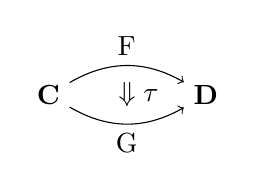
\begin{tikzpicture}
    \node (C) at (-1,0) {$\cat{C}$};
    \node (D) at (1,0) {$\cat{D}$};
    \node (T) at (0,0) {$\;\;\;\Downarrow\tau$};
    \draw[->,bend left] (C) to node [above] {F} (D);
    \draw[->,bend right] (C) to node [below] {G} (D);
  \end{tikzpicture}
\]
such that:
\begin{enumerate}
  \item $\forall X \in \cat{C},
    \exists \tau_X : F(X) \rightarrow G(X) \in \cat{D}$
  \item $\forall f : X \rightarrow Y \in \cat{C},
    \tau_Y \circ F(f) = G(f) \circ \tau_X$
\end{enumerate}
where the Morphism $\tau_X$ is called the \emph{Component} of $\tau$
at $X$. When (2) holds, a Commutative Diagram is formed and the
Morphisms $\tau_X$ are said to be \emph{Natural} in $X$. If there is
no Morphism in $\cat{D}$ corresponding to $\tau_X$, then there can
be no Natural Transformation from $F$ to $G$.

Milewski: A Natural Transformation maps Morphisms to Commuting
Diagrams

When every Component in $\tau$ is Invertible in $\cat{D}$, $\tau$ is a
\emph{Natural Isomorphism} (\S\ref{sec:natural_isomorphism}) and $F
\cong G$. Equivalently, a Natural Isomorphism is an Isomorphism in the
Functor Category $Fun(\cat{C},\cat{D})$.

Natural Isomorphisms:
\[
  Hom_\cat{Grp}(F_1,G) \cong U(G)
\]\[
  Hom_\cat{Set}(X,\cat{2}) \cong \pow(X)
\]\[
  Hom_\cat{BA}(B,\cat{2}) \cong Ult(X)
\]

in Programming Languages, Natural Transformations may be represented
as Polymorphic Functions (i.e. Family of Functions Parameterized by
Types)

Horizontal Composition (\S\ref{sec:horizontal_composition}):
Composition along $1$-morphisms (Functors)

Vertical Composition (\S\ref{sec:horizontal_composition}):
Composition along Objects (Categories)



% --------------------------------------------------------------------
\subsection{Vertical Composition}\label{sec:vertical_composition}
% --------------------------------------------------------------------

Given Natural Transformations $\eta : F \Rightarrow G$ and $\epsilon :
G \Rightarrow H$ between Functors $F,G,H : \cat{C} \rightarrow
\cat{D}$, the \emph{Vertical Composition} is $\epsilon\circ\eta : F
\Rightarrow H$:
\[
  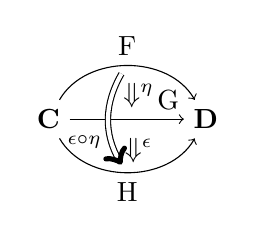
\begin{tikzpicture}
    \node (C) at (-1,0) {$\cat{C}$};
    \node (D) at (1,0) {$\cat{D}$};
    \node (N) at (0,0.3) {$\;\;\;\Downarrow^\eta$};
    \node (M) at (0,-0.4) {$\;\;\;\Downarrow^\epsilon$};
    \node (F) at (0,0.7) {};
    \node (H) at (0,-0.7) {};
    \draw[->,bend left=60] (C) to node [above] {F} (D);
    \draw[->] (C) to node [above] {\quad\quad\quad G} (D);
    \draw[->,bend right=60] (C) to node [below] {H} (D);
    \draw[->,bend right=30,double distance=1.5pt] (F) to
      node [left,pos=0.75] {$_{\epsilon\circ\eta}$} (H);
  \end{tikzpicture}
\]

Composition in the corresponding Functor Category



% --------------------------------------------------------------------
\subsection{Horizontal Composition}\label{sec:horizontal_composition}
% --------------------------------------------------------------------

Given Functors $F,G : \cat{C} \rightarrow \cat{D}$ and $J,K : \cat{D}
\rightarrow \cat{E}$, and Natural Transformations $\eta : F
\rightarrow G$ and $\epsilon : J \rightarrow K$, the \emph{Horizontal
  Composition} (or \emph{Godement Product}) is $\eta * \epsilon : JF
\Rightarrow KG$:
\[
  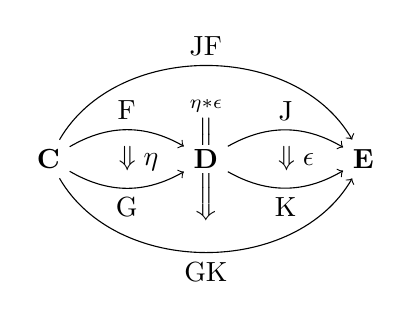
\begin{tikzpicture}
    \node (U) at (0,0) {$\stackrel{\eta*\epsilon}
      {\stackrel{\Big\|}{\Big\Downarrow}}$};
    \node [fill,color=white,scale=1.5] (W) at (0,0) {};
    \node (C) at (-2,0) {$\cat{C}$};
    \node (D) at (0,0) {$\cat{D}$};
    \node (E) at (2,0) {$\cat{E}$};
    \node (S) at (-1,0) {$\;\;\;\Downarrow\eta$};
    \node (T) at (1,0) {$\;\;\;\Downarrow\epsilon$};
    \draw[->,bend left] (C) to node [above] {F} (D);
    \draw[->,bend right] (C) to node [below] {G} (D);
    \draw[->,bend left] (D) to node [above] {J} (E);
    \draw[->,bend right] (D) to node [below] {K} (E);
    \draw[->,bend left=60] (C) to node [above] {JF} (E);
    \draw[->,bend right=60] (C) to node [below] {GK} (E);
  \end{tikzpicture}
\]

Horizontal Composition is Associative and has the same Identity as
Vertical Composition.



% --------------------------------------------------------------------
\subsection{Interchange Law}\label{sec:interchange_law}
% --------------------------------------------------------------------

Given three Categories, $\cat{B}$, $\cat{C}$, and $\cat{D}$,
and six Functors, $P,Q,R : \cat{B} \rightarrow \cat{C}$ and
$S,T,U : \cat{C} \rightarrow \cat{D}$, and four Natural
Transformations, $\sigma : P \rightarrow Q$, $\tau : Q \rightarrow R$,
$\sigma' : S \rightarrow T$, and $\tau' : T \rightarrow U$, the
following \emph{Interchange Law} applies:
\[
  (\tau' \cdot \sigma') \circ (\tau \cdot \sigma) =
  (\tau' \circ \tau) \cdot (\sigma' \circ \sigma)
\]



% --------------------------------------------------------------------
\subsection{Natural Isomorphism}\label{sec:natural_isomorphism}
% --------------------------------------------------------------------

\emph{Natural Equivalence} in a $1$-category %FIXME xref

\[
  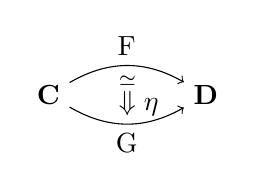
\begin{tikzpicture}
    \node (C) at (-1,0) {$\cat{C}$};
    \node (D) at (1,0) {$\cat{D}$};
    \node (N) at (0,0) {$\;\;\;\stackrel{\simeq}{\Downarrow}\eta$};
    \draw[->,bend left] (C) to node [above] {F} (D);
    \draw[->,bend right] (C) to node [below] {G} (D);
  \end{tikzpicture}
\]

\begin{itemize}
  \item Natural Isomorphism with a Two-sided Inverse (???)
  \item each Component $\eta_X : F(X) \rightarrow G(X)$ for all $X
    \in \cat{C}_0$ is an Isomorphism in $\cat{D}$
  \item Isomorphism in the Functor Category
    (\S\ref{sec:functor_category}) $[\cat{C},\cat{D}]$
\end{itemize}



% --------------------------------------------------------------------
\subsection{Extranatural Transformation}
\label{sec:extranatural_transformation}
% --------------------------------------------------------------------

For Functors $F : \cat{A} \times \cat{B}^{op} \times \cat{B}
\rightarrow \cat{D}$ and $G : \cat{A} \times \cat{C}^{op} \times
\cat{C} \rightarrow \cat{D}$, the Family $\eta(a,b,c) : F(a,b,b)
\rightarrow G(a,c,c)$ is Natural in $a$ and \emph{Extranatural} in $b$
and $c$ if the following holds:
\begin{itemize}
  \item (Natural in $a$): $\eta (-,b,c)$ is a Natural Transformation
  \item (Extranatural in $b$): $\forall (g:b \rightarrow b') \in
    \cat{B}_1, \forall a \in \cat{A}, \forall c \in \cat{C},
    \eta(a,b,c) \circ F(1,1,g) = \eta(a,b',c) \circ F(1,g,1)$
  \item (Extranatural in $c$): $\forall (h:c \rightarrow c') \in
    \cat{C}_1, \forall a \in \cat{A}, \forall b \in \cat{B}, G(1,h,1)
    \circ \eta(a,b,c) = G(1,1,h) \circ \eta(a,b,c')$
\end{itemize}



% --------------------------------------------------------------------
\subsection{Dinatural Transformation}
\label{sec:dinatural_transformation}
% --------------------------------------------------------------------

Ex.: Hughes Arrow (\S\ref{sec:hughes_arrow}) $\ggg : A (X,P) \times A
(P,Y) \rightarrow A (X,Y)$ is Dinatural in $P$. For each $f : P
\rightarrow Q$:
\[
  id \times A(f,id) \circ \ggg = A(id,f) \times id \circ \ggg
\]



% ====================================================================
\section{Opposite Category}\label{sec:opposite_category}
% ====================================================================

The \emph{Opposite} or \emph{Dual} (\S\ref{sec:abstract_category})
of a Category $\cat{C}$ is denoted $\cat{C^{op}}$ or
$\cat{C^*}$ and has the same Objects as $\cat{C}$ but the Domain
and Codomain in each Morphism is reversed. Objects and Morphisms of a
Dual Category may be written with over-lines to distinguish them from
the original Category: $\overline{f}: \overline{C} \rightarrow
\overline{D}$. With this notation the following Equalities may be
expressed:
\[
  1_{\overline{C}} = \overline{1_C}
\]\[
  \overline{f} \circ \overline{g} = \overline{g \circ f}
\]
A Terminal Object in $\cat{C}$ is an Initial Object in
$\cat{C^{op}}$ and vice-versa.

The Functor $(-)^\cat{op} : \cat{Cat} \rightarrow \cat{Cat}$
is an Involution (\S\ref{sec:involution}) but is Contravariant so it
does not define any Isomorphisms.

In a Dual Category the following are all Duals of eachother:
\begin{itemize}
  \item Monomorphisms and Epimorphisms (\S\ref{sec:morphism})
  \item Left and Right Inverses (\S\ref{sec:morphism})
  \item Initial and Terminal Objects (\S\ref{sec:universal_property})
\end{itemize}



% ====================================================================
\section{Category Product}\label{sec:category_product}
% ====================================================================

A \emph{Product}, $\times$, is a Construction (i.e. a Functor,
specifically a Bifunctor \S\ref{sec:bifunctor}) on Categories (or
Functors):
\[
  \times : \cat{Cat} \times \cat{Cat} \rightarrow \cat{Cat}
\]

Product (\S\ref{sec:product})



% --------------------------------------------------------------------
\subsection{Product Category}\label{sec:product_category}
% --------------------------------------------------------------------

A \emph{Product Category} can be constructed from two Categories,
$\cat{C}$ and $\cat{D}$, and is denoted:
\[
  \cat{C} \times \cat{D}
\]
has Objects of the form $(C,D)$ where $C \in \cat{C}$ and $D \in
\cat{D}$ and Morphisms $(f,g) : (C,D) \rightarrow (C',D')$ where $f
: C \rightarrow C' \in \cat{C}$ and $g : D \rightarrow D' \in
\cat{D}$. Composition and Identity are defined as:
\[
  (f',g') \circ (f,g) = (f' \circ f,g' \circ g)
\]\[
  1_{(C,D)} = (1_C, 1_D)
\]
$\cat{C} \times \cat{D}$ is a Product (\S\ref{sec:product}) in
$\cat{Cat}$.



\subsubsection{Projection}\label{sec:projection_functor}

A Product Category has a pair of \emph{Projections} which are Functors
from the Product Category to the original Categories:
\[
  \cat{C} \xleftarrow{\;\; P\;\;} \cat{C}\times\cat{D}
  \xrightarrow{\;\; Q\;\;} \cat{D}
\]
such that for $C,f \in \cat{C}, D,g \in \cat{D}$:
\[
  P(C,D) = C, \;\; P(f,g) = f
\]\[
  Q(C,D) = D, \;\; Q(f,g) = g
\]
Given any other Category, $\cat{B}$, there exists a unique Functor:
\[
  F : \cat{B} \rightarrow \cat{C} \times \cat{D}
\]
with:
\[
  PF = R : \cat{B} \rightarrow \cat{C}
\]\[
  QF = T : \cat{B} \rightarrow \cat{D}
\]
giving:
\[
  \forall h \in B, F(h) = (Rh,Th)
\]



% --------------------------------------------------------------------
\subsection{Functor Product}\label{sec:functor_product}
% --------------------------------------------------------------------

Give two Functors, $U : \cat{C} \rightarrow \cat{C'}$ and $V :
\cat{D} \rightarrow \cat{D'}$, a \emph{Functor Product} is
defined as:
\[
  U \times V : \cat{C} \times \cat{D}
  \rightarrow \cat{C'} \times \cat{D'}
\]
where:
\[
  (U \times V)(C,D) = (UC,VD), \;\; (U \times V)(f,g) = (Uf,Vg)
\]
and $(U \times V)$ is the unique Functor such that:
\[
  P'(U \times V) = UP, \;\; Q'(U \times V) = VQ
\]
%FIXME is the above correct?



% ====================================================================
\section{Quotient Category}\label{sec:quotient_category}
% ====================================================================

%FIXME this probably needs a rewrite

The \emph{Quotient Category} is defined for a Category $\cat{C}$
with Congruence Relation $\sim$ as $\cat{C}/\sim$:
\[
  (\cat{C}/\sim)_0 = \cat{C_0}
\]\[
  (\cat{C}/\sim)_1 = (\cat{C_1})/\sim
\]
where Morphisms are of the form $[f]$ where $f \in \cat{C_1}$.

For a Category $\cat{C}$ with Graph $G$ and relations $R$,
$\cat{C}/R$ is called the Category with \emph{Generators} $G$ and
\emph{Relations} $R$.

Homotopy Category (\S\ref{sec:homotopy_category})



% --------------------------------------------------------------------
\subsection{Congruence Category}\label{sec:congruence_category}
% --------------------------------------------------------------------

\emph{Congruence} on a Category is an Equivalence Relation on
Morphisms such that for two Morphisms $f,g \in \cat{C_1}$, $f \sim
g$ Implies:
\begin{itemize}
  \item $dom(f) = dom(g)$
  \item $cod(f) = cod(g)$
  \item $\forall a,b \in \cat{C_1}, bfa \sim bga$
\end{itemize}
Such a Congruence defines a \emph{Congruence Category}
$\cat{C^{\sim}}$:
\[
  (\cat{C^{\sim}})_0 = \cat{C}_0
\]\[
  (\cat{C^{\sim}})_1 = \{\langle f,g \rangle | f \sim g\}
\]\[
  \tilde{1_\cat{C}} = \langle 1_\cat{C}, 1_\cat{C} \rangle
\]\[
  \langle f',g' \rangle \circ \langle f,g \rangle = \langle f'f,g'g \rangle
\]
The Categorical Congruence $\sim$ on a Group $G$ is a Normal Subgroup
$N \subseteq G$ and the Quotient Category $G/\sim$ and the Quotient
Group $G/N$ coincide. \cite{awodey06}



% --------------------------------------------------------------------
\subsection{Kernel Category}\label{sec:kernel_category}
% --------------------------------------------------------------------

Given a Functor $F : \cat{C} \rightarrow \cat{D}$, a Congruence
$\sim_F$ on $\cat{C}$ is defined as:
\[
  f \sim_F g \leftrightarrow dom(f) = dom(g) \wedge cod(f) = cod(g)
  \wedge F(f) = F(g)
\]
The \emph{Kernel Category} of $F$ is then defined as the Congruence
Category of $\sim_F$
\[
  ker(F) = C^{\sim_F}
\]



% --------------------------------------------------------------------
\subsection{Finitely Presented Category}
\label{sec:finitely_presented}
% --------------------------------------------------------------------

% FIXME free category notation?
A \emph{Finitely Presented Category} is given by taking the Quotient
Category of a Free Category (\S\ref{sec:free_category})
$\cat{C}(G)$ with the Congruence $\sim_\Sigma$:
\[
  \cat{C}(G) / \sim_{\Sigma} = \cat{C}(G,\Sigma)
\]
where $\Sigma$ is the finite Set of Relations:
\[
  (g_1 \circ \ldots \circ g_n) = (g'_1 \circ \ldots \circ g'_m)
\]
for all $g_i \in G$ such that $dom(g_n) = dom(g'_m)$ and $cod(g_1) =
cod(g'_1)$.



% ====================================================================
\section{Arrow Category}\label{sec:arrow_category}
% ====================================================================

An \emph{Arrow Category} of a Category $\cat{C}$, written
$\cat{C^{\rightarrow}}$, has for its Objects the Morphisms of
$\cat{C}$ and as Morphisms pairs of Objects such that their
underlying Morphisms in $\cat{C}$ are Composable (Commutative
Squares).

The Arrow Category $\cat{C}^\rightarrow$ is Isomorphic to the
Functor Category $\cat{C^2}$.

There are two Functors defined on an Arrow Category:
\[
  \cat{C} \xleftarrow{\cat{dom}} \cat{C}^\rightarrow
  \xrightarrow{\cat{cod}} \cat{D}
\]

Equivalent to the Comma Category (\S\ref{sec:comma_category})
$(1_\cat{C}/1_\cat{C})$



% ====================================================================
\section{Comma Category}\label{sec:comma_category}
% ====================================================================

A \emph{Comma Category} is formed from a pair of Functors that share a
common Codomain. For three Categories, $\cat{A}$, $\cat{B}$, and
$\cat{C}$ and Functors $S$ (\emph{Source}) and $T$ (\emph{Target}) in
the following relation:
\[
  \cat{A} \xrightarrow{\;\; S\;\;} \cat{C} \xleftarrow{\;\;
    T\;\;} \cat{B}
\]
one can form a Comma Category $(S \downarrow T)$ with Objects as
Triples $(\alpha, \beta, f)$ where $\alpha$ is an Object in
$\cat{A}$, $\beta$ is an Object in $\cat{B}$, and $f : S(\alpha)
\rightarrow T(\beta)$ is a Morphism in $\cat{C}$ and with Morphisms
between Triples $(\alpha, \beta, f)$ to $(\alpha', \beta', f')$ as
pairs $(g,h)$ where $g : \alpha \rightarrow \alpha'$ is a Morphism in
$\cat{A}$ and $h : \beta \rightarrow \beta'$ is a Morphism in
$\cat{B}$.

When $S$ is a Functor, $\cat{1} \xrightarrow{\;\;S\;\;}
\cat{C}$, to a single Object $A \in \cat{C}$, the resulting
Comma Category may be denoted $(A \downarrow \cat{C})$ and is
called the Category of Objects under $A$. Here Objects are Morphisms
with Domain of $A$, and Morphisms are Commutative triangles with top
Vertex $A$.

The Category of Objects over $A$ is likewise $(\cat{C} \downarrow
A)$ and has as Objects Morphisms with Codomain $A$ and Morphisms are
Commutative triangles with a bottom Vertex $A$.

When both $S$ and $T$ are Functors from $\cat{1}$ to Objects $A$
and $B$ respectively, the result is a Discrete Category whose Objects
are $Hom(A,B)$.

The case where $S = T = 1_\cat{C}$, $(\cat{C} \downarrow
\cat{C})$, is the Category of all Morphisms of $\cat{C}$:
$\cat{C}^\cat{2}$.



% --------------------------------------------------------------------
\subsection{Slice Category}\label{sec:slice_category}
% --------------------------------------------------------------------

A \emph{Slice Category} (or \emph{Overcategory}) $\cat{C}/C$ of a
Category $\cat{C}$ with an Object $C$ has as Objects the Morphisms
with Codomain $C$ and as Morphisms those Morphisms in $\cat{C}$
between the Domains of the underlying Morphisms of the Objects of
$\cat{C}/C$. That is, for Objects in the Slice Category corresonding
to Morphisms $f$ and $f'$, the Morphism in the Slice Category between
the two is $g$ such that
\[
  f' \circ g = f
\]

\emph{Coslice}

if each Slice Category $\cat{C}/x$ is a Cartesian Monoidal Category
(\S\ref{sec:cartesian_monoidal}) then $\cat{C}$ is Locally Cartesian
(\S\ref{sec:locally_cartesian})

Categorical Semantics (\S\ref{sec:categorical_semantics}) for Formal
Logic (Part \ref{part:formal_logic}) and Type Theory (Part
\ref{part:type_theory})



% --------------------------------------------------------------------
\subsection{Coslice Category}\label{sec:coslice_category}
% --------------------------------------------------------------------



% ====================================================================
\section{Bifunctor}\label{sec:bifunctor}
% ====================================================================

A \emph{Bifunctor} is a Functor of two Variables from a Product
Category to an arbitrary Category:
\[
  B : \cat{C} \times \cat{D} \rightarrow \cat{A}
\]

A \emph{Multifunctor} is a generalized to $n$ or more Variables.



% --------------------------------------------------------------------
\subsection{Product Functor}\label{sec:product_functor}
% --------------------------------------------------------------------

\[
  \times : \cat{C} \times \cat{C} \rightarrow \cat{C}
\]

Category Product (\S\ref{sec:category_product})



% --------------------------------------------------------------------
\subsection{Coproduct Functor}\label{sec:coproduct_functor}
% --------------------------------------------------------------------

\[
  + : \cat{C} \times \cat{C} \rightarrow \cat{C}
\]



% --------------------------------------------------------------------
\subsection{Diagonal Functor}\label{sec:diagonal_functor}
% --------------------------------------------------------------------

For Functor Category (\S\ref{sec:functor_category})
$\cat{C}^\cat{J}$ with Small Index Category $\cat{J}$, a
\emph{Diagonal Functor} $\Delta : \cat{C} \rightarrow
\cat{C}^\cat{J}$ assigns to each Object $A$ of $\cat{C}$ the
Constant Functor $\Delta_A \in \cat{C}^\cat{J}$ with fixed $A$
and to each Morphism $f : A \rightarrow B$ of $\cat{C}$ the Natural
Transformation $\eta$ in $\cat{C}^\cat{J}$ given by $\eta_j =
f$.

If $\cat{J}$ is a Discrete Category with two Objects, the Diagonal
Functor is $\cat{C} \rightarrow \cat{C} \times \cat{C}$.

The Limit (\S\ref{sec:limit}) of a Functor $F : \cat{J} \rightarrow
\cat{C}$ is a Universal Morphism (\S\ref{sec:universal_morphism})
from the Diagonal Functor $\Delta$ to $F$.

If $\cat{C}$ is Complete (\S\ref{sec:complete_category}) then every
Functor from $\cat{J}$ to $\cat{C}$ has a Limit and the
operation of taking Limits is a Functor from $\cat{C}^\cat{J}$
to $\cat{C}$.

The Limit Functor is the Right-adjoint (\S\ref{sec:adjoint_functor})
of the Diagonal Functor.

A Colimit (\S\ref{sec:colimit}) is a Universal Morphism $F \rightarrow
\Delta$.

If $\cat{C}$ is Complete the Colimit Functor exists and is the
Left-adjoint of the Diagonal Functor.

As an example, the Diagonal Functor $\cat{C} \rightarrow \cat{C}
\times \cat{C}$ is the Left-adjoint of the Binary Product Functor
(\S\ref{sec:product_functor}) and the Right-adjoint of the Binary
Coproduct Functor (\S\ref{sec:coproduct_functor}).



% --------------------------------------------------------------------
\subsection{Profunctor}\label{sec:profunctor}
% --------------------------------------------------------------------

A \emph{Profunctor} (or \emph{Distributor}) is a Bifunctor that is
Contravariant in the first argument and Covariant in the second.

Generalization of Functors, Categorical generalization of Bimodules
(\S\ref{sec:bimodule})

$P : \cat{C} \nrightarrow \cat{D}$

$H_P : \cat{D}^{op} \times \cat{C} \rightarrow \cat{Set}$

Set of Heteromorphisms (\S\ref{sec:heteromorphism})

Identity Profunctor $Id : \cat{C} \nrightarrow \cat{C}$ is given by
the Hom-functor $\cat{C}(-,-) : \cat{C}^{op} \times \cat{C}
\rightarrow \cat{Set}$

Composition of Profunctors $P : \cat{C} \nrightarrow \cat{D}$, $Q :
\cat{D} \nrightarrow \cat{E}$:
\[
  Q P = \int^{d \in \cat{D}} P(d,-) \otimes Q(-,d)
\]
% FIXME kan extensions?

Every Functor $F : \cat{C} \rightarrow \cat{D}$ induces two
Profunctors $D(1,F) : \cat{C} \nrightarrow \cat{D}$ and $D(F,1)
: \cat{D} \nrightarrow \cat{C}$ where $D(1,F)(d,c) = D(d,f(c))$
and $D(f,1)(c,d) = D(f(c),d)$.

Functor $F : \cat{C} \rightarrow \cat{D}$ gives a Profunctor $P_F :
\cat{C} \nrightarrow \cat{D}$ by Post-composition with the Yoneda
Functor (\S\ref{sec:yoneda_embedding}):
\[
  P_F = Y_\cat{D} \circ F
\]



\subsubsection{Profunctor Bicategory}\label{sec:profunctor_bicategory}

Bicategory (\S\ref{sec:bicategory}) of Profunctors

Coend (\S\ref{sec:coend})



% ====================================================================
\section{Hom-functor}\label{sec:hom_functor}
% ====================================================================

A \emph{Hom-functor} is a Functor from a Locally Small Category
(\S\ref{sec:locally_small}), $\cat{C}$, to the Category $\cat{Set}$,
and has a Covariant and a Contravariant definition:

\begin{enumerate}
  \item \emph{Covariant Hom-functor}, for $A \in \cat{C}_0$, $f : X
    \rightarrow Y \in \cat{C}_1$:
\[
\begin{split}
  & h^A = Hom(A,-) : \cat{C} \rightarrow \cat{Set} \\
  & X \mapsto Hom(A,X) \\
  & f \mapsto Hom(A,f) : Hom(A,X) \rightarrow Hom(A,Y)
\end{split}
\]
  where $Hom(A,f)$ is defined for all $g \in Hom(A,X)$ as:
\[
  g \mapsto f \circ g
\]

  \item \emph{Contravariant Hom-functor} (also \emph{Functor of
    Points}, see Generalized Elements
    \S\ref{sec:generalized_element}), for $B \in \cat{C}_0$, $f : X
    \rightarrow Y \in \cat{C}_1$:
\[
\begin{split}
  & h_B = Hom(-,B) : \cat{C} \rightarrow \cat{Set} \\
  & X \mapsto Hom(X,B) \\
  & f \mapsto Hom(f,B) : Hom(Y,B) \rightarrow Hom(X,B)
\end{split}
\]
  where $Hom(f,B)$ is defined for all $g \in Hom(Y,B)$ as:
\[
  g \mapsto g \circ f
\]
\end{enumerate}

The Hom-functor $Hom(-,-)$ is a Covariant Bifunctor
(\S\ref{sec:bifunctor}):
\[
  Hom_\cat{C}(-,-):
    \cat{C}^{op} \times \cat{C} \rightarrow \cat{Set}
\]
each half of which is a Representable Functor
(\S\ref{sec:representable_functor}). $Hom_\cat{C}(-,-)$ is also the
Identity Profunctor (\S\ref{sec:profunctor}) $1_\cat{C} :
\cat{C} \nrightarrow \cat{C}$. Hom-functors are Continuous
Functors (\S\ref{sec:continuous_functor}).

The Category of all Hom-functors and Natural Transformations
(\S\ref{sec:natural_transformation}) between them, $\{ h^A | A \in
\cat{C} \}$, is a Subcategory of the Functor Category
(\S\ref{sec:functor_category}) $\cat{Set^C}$, and is Isomorphic to
$\cat{C^{op}}$ (see Yoneda Embedding \S\ref{sec:yoneda_embedding}).

Every Morphism $f : A' \rightarrow A$ determines a pair of Natural
Transformations:
\[
  Hom(f,-) : h^A \rightarrow h^{A'}
\]\[
  Hom(-,f) : h_{A'} \rightarrow h_A
\]

For any pair of Morphisms, $f : A' \rightarrow A$ and $g : B
\rightarrow B'$:
\[
  Hom(A',g) \circ Hom(f,B) = Hom(f,B') \circ Hom(A,g)
\]
is a path sending:
\[
  h : A \rightarrow B
\]
to:
\[
  g \circ h \circ f : A' \rightarrow B'
\]



% --------------------------------------------------------------------
\subsection{Closed Category}\label{sec:closed_category}
% --------------------------------------------------------------------

A \emph{Closed Category} is a Category $\cat{C}$ with:
\begin{itemize}
  \item Internal Hom-functor (\S\ref{sec:internal_hom}):
    \[
      [-,-]:\cat{C}^{op} \times \cat{C} \rightarrow \cat{C}
    \]
  \item Unit Object:
    \[
      I \in \cat{C}_0
    \]
  \item Natural Isomorphism:
    \[
      i : 1_\cat{C} \cong [I,-]
    \]
  \item Transformation:
    \[
      j_X : I \rightarrow [X,X]
    \]
    Extranatural (\S\ref{sec:extranatural_transformation}) in $X$
  \item Transformation:
    \[
      L_{Y Z}^X : [Y,Z] \rightarrow [[X,Y],[X,Z]]
    \]
    Natural in $Y$ and $Z$ and Extranatural in $X$
\end{itemize}
Satisfying the Axioms:
\begin{enumerate}
  \item $L_{Y Y}^X \circ j_Y = j_{[X,Y]}$ for any $X,Y$
  \item $[j_X,1] \circ L_{X Y}^X = i_{[X,Y]}$ for any $X,Y$
  \item $[i_Y,1] \circ L_{Y Z}^I = [1,i_Z]$ for any $Y,Z$
  \item $[1,L_{Y V}^X] \circ L_{U V}^Y = [L_{Y U}^X,1] \circ L_{[X,U]
    [X,V]}^{[X,Y]} \circ L_{U V}^X$ for any $X,Y,U,V$
  \item The Map $\gamma : \cat{C}(X,Y) \rightarrow \cat{C}(I,[X,Y])$
    defined by $f \mapsto [1,f](j_X)$ is a Bijection
\end{enumerate}

Every Closed Category embeds Fully and Faithfully into a Closed
Monoidal Category (\S\ref{sec:closed_monoidal}) by a Strong Closed
Functor (LaPlaza) %FIXME



\subsubsection{Internal Hom-functor}\label{sec:internal_hom}

\emph{Internal Hom Functor}
\[
  [-,-] : \cat{C}^{op} \times \cat{C} \rightarrow \cat{C}
\]



\subsubsection{Dualizing Object}\label{sec:dualizing_object}

\emph{Dualizing Object} $D$ in a Closed Category $\cat{D}$ is an
Object with Internal Hom $[-,D]: \cat{C} \rightarrow \cat{C}^{op}$ an
Involutive Duality Operation on $\cat{C}$: %FIXME
\[
  [[-,D],D]: \cat{C} \rightarrow \cat{C}
\]

Dual Object (\S\ref{sec:dual_object})



% --------------------------------------------------------------------
\subsection{Representable Functor}\label{sec:representable_functor}
% --------------------------------------------------------------------

%FIXME definition of 'representation'
%FIXME ref Naturally Isomorphic
Presheaf (\S\ref{sec:category_presheaf})

A Functor $F : \cat{C} \rightarrow \cat{Set}$ is a
\emph{Representable Functor} if it is Naturally Isomorphic to the
Hom-functor $h^A$ or $h_A$ for some Object $A \in \cat{C}$.

A \emph{Covariant Representable Functor} for an Object $A$ in a
Category $\cat{C}$ is defined as Naturally Isomorphic to the
Covariant Hom-functor $h^A = Hom(A,-) : \cat{C} \rightarrow
\cat{Set}$
\[
  Hom(A,-) : Hom(A,X) \xrightarrow{f_*} Hom(A,Y)
\]
A \emph{Contravariant Representable Functor} for $A$ is a Functor that
is Naturally Isomorphic to the Contravariant Hom-functor $h_A =
Hom(-,A) : \cat{C^{op}} \rightarrow \cat{Set}$
\[
  Hom(-,A) : Hom(X,A) \xrightarrow{f^*} Hom(Y,A)
\]

A \emph{Representation} of a Covariant Representable Functor, $F$, is
a pair $(A, \Phi)$ with Natural Isomorphism $\Phi : Hom(A,-)
\rightarrow F$.

Contravariant Representable Functors map all Colimits
(\S\ref{sec:colimit}) to Limits (\S\ref{sec:limit}).

A Locally Small Category (\S\ref{sec:locally_small}) has Representable
Functors for all Objects.

generalization of Upper Sets (\S\ref{sec:upper_set}) in Posets



% --------------------------------------------------------------------
\subsection{Locally Small Category}\label{sec:locally_small}
% --------------------------------------------------------------------

A Category is \emph{Locally Small} if all Hom-sets
(\S\ref{sec:hom_set}) of the Category are Sets and not Proper Classes.
% FIXME definition in terms of hom-sets

Hom-functor (\S\ref{sec:hom_functor})

There is at least one canonical Representable Functor
(\S\ref{sec:representable_functor}) from any Locally Small Category
into $\cat{Set}$.

For a Locally Small Category $\cat{C}$, $\cat{Set^{C^{op}}}$ is
Complete (\S\ref{sec:complete_category}) and Cocomplete
(\S\ref{sec:cocomplete_category}) and for all $C \in \cat{C}_0$,
the Evaluation Functor $ev_C : \cat{Set^{C^{op}}} \rightarrow
\cat{Set}$ preserves all Limits. \cite{awodey06}



% ====================================================================
\section{Concrete Category}\label{sec:concrete_category}
% ====================================================================

A \emph{Concrete Category} is pair, $(\cat{C},U)$, where $\cat{C}$ is
a Category and $U$ is a Faithful Functor
(\S\ref{sec:faithful_functor}) $U : \cat{C} \rightarrow \cat{Set}$.

Representable Functor (\S\ref{sec:representable_functor})

Sets with Structure (\S\ref{sec:abstract_structure})

Categories with Interpretations as Concrete Categories:
\begin{itemize}
  \item $\cat{Set}$
  \item $\cat{Top}$
  \item $\cat{Grp}$
\end{itemize}

Not \emph{Concretizable}:
\begin{itemize}
  \item $\cat{Toph}$
\end{itemize}



% ====================================================================
\section{Yoneda Lemma}\label{sec:yoneda_lemma}
% ====================================================================

For an arbitrary Covariant Functor $F : \cat{C} \rightarrow
\cat{Set}$:
\[
  Nat_\cat{Set^C}(h^A,F) \cong F(A)
\]
If $F$ is a Covariant Hom-functor $h^B$, then:
\[
  Nat_\cat{Set^C}(h^A,h^B) \cong Hom(B,A)
\]

For an arbitrary Contravariant Functor $G : \cat{C}^{op} \rightarrow
\cat{Set}$:
\[
  Nat_\cat{Set^{C^op}}(h_B,G) \cong G(A)
\]
If $F$ is a Contravariant Hom-functor $h_B$, then:
\[
  Nat_\cat{Set^{C^{op}}}(h_A,h_B) \cong Hom(A,B)
\]

Corollary:
\[
  yA \cong yB \Rightarrow A \cong B
\]



% --------------------------------------------------------------------
\subsection{Yoneda Embedding}\label{sec:yoneda_embedding}
% --------------------------------------------------------------------

The Fully Faithful Contravariant Functor $h^- : \cat{C} \rightarrow
\cat{Set^C}$ which maps each Object $A \in \cat{C}_0$ to the
Hom-functor $h^A$ and each $f \in \cat{C}_1$ to the Natural
Transformation $Hom(f,-)$ can also be interpreted as a Covariant
Functor $h^- : \cat{C^{op}} \rightarrow \cat{Set^C}$. Being a
Faithful Functor means $h^-$ gives an Embedding
(\S\ref{sec:category_embedding}) of $\cat{C^{op}}$ in
$\cat{Set^C}$.

By the Contravariant Yoneda's Lemma:
\[
  h_-: \cat{C} \rightarrow \cat{Set^{C^{op}}}
\]
called the \emph{Yoneda Embedding}.

Covariant:

$Nat_\cat{Set^C}(Hom(A,-), Hom(B,-)) \cong Hom_\cat{C}(B,A)$

Contravariant:

$Nat_\cat{Set^{C^op}}(Hom(-,A), Hom(-,B)) \cong Hom_\cat{C}(A,B)$

Yoneda Embedding preserves all Products and Exponentials in
$\cat{C}$.



% --------------------------------------------------------------------
\subsection{Coyoneda}\label{sec:coyoneda}
% --------------------------------------------------------------------

Free Functor (\S\ref{sec:free_functor})



% ====================================================================
\section{Functor Category}\label{sec:functor_category}
% ====================================================================

Given two Categories, $\cat{C}$ and $\cat{D}$, a \emph{Functor
  Category} is a Category with Objects as Functors $T : \cat{C}
\rightarrow \cat{D}$ and Morphisms as Natural Transformations
between Functors:
\[
  \cat{D}^{\cat{C}} = Fun(\cat{C},\cat{D})
\]

$[\cat{C},\cat{D}]$

A Hom-set in a Functor Category may be denoted:
\[
  Nat(S,T) = \cat{D}^{\cat{C}}(S,T) =
    \{ \tau | \tau : S \rightarrow T \}
\]

With Evaluation Functor $\eta : \cat{D^C} \times \cat{C} \rightarrow
\cat{D}$, $\cat{D^C}$ is an Exponential
(\S\ref{sec:category_exponential}) in $\cat{Cat}$ and $\cat{Cat}$ is a
Cartesian Closed Category (\S\ref{sec:cartesian_closed}).

The Functor Category $\cat{C^2}$ is Isomorphic to Arrow Categories
(\S\ref{sec:arrow_category}) $\cat{C}^\rightarrow$.

The Functor Category $\cat{C}^\cat{2}$ from the Discrete Category
$\cat{2}$ is equivalent to the Product Category $\cat{C} \times
\cat{C}$.

For any Discrete Category $I$:
\[
  \cat{C}^I \cong \prod_{i \in I} \cat{C}
\]

The Functor Category $\cat{Set}^\downdownarrows$ where
$\downdownarrows$ is the Category with two Objects and two Morphisms
between them ($* \rightrightarrows \star$) is equivalent to the
Category of Graphs and Graph Homomorphisms $\cat{Graph}$. Cf.
Simplicial Sets (\S\ref{sec:simplicial_set}).

A Functor Category into the Category $\cat{Set}$ is called a
\emph{Category Diagram} (\S\ref{sec:category_diagram}).
%FIXME terminology doesn't match



% --------------------------------------------------------------------
\subsection{Set-valued Functor Category}\label{sec:setvalued_functor}
% --------------------------------------------------------------------

A \emph{Set-valued Functor Category} (or \emph{Category of Diagrams})
is a Functor Category from a Category into the Category
$\cat{Set}$.

A Presheaf (\S\ref{sec:presheaf}) is an example of a Set-valued
(Contravariant) Functor Category from an Opposite Category into
$\cat{Set}$.



\subsubsection{Powerset Functor}\label{sec:powerset_functor}

$\pow : \cat{Set} \rightarrow \cat{Set}$

Functions $f : X \rightarrow Y$ to the Image Mapping $img(f) :
\pow(X) \rightarrow \pow(Y)$



% ====================================================================
\section{Presheaf Category}\label{sec:presheaf_category}
% ====================================================================

Objects: Functors $F: \cat{C}^{op} \rightarrow \cat{Set}$

Morphisms: Natural Transformations $\Phi : F \rightarrow G$

$Psh(\cat{C}) = [\cat{C}^{op},\cat{Set}]$



% --------------------------------------------------------------------
\subsection{Presheaf}\label{sec:category_presheaf}
% --------------------------------------------------------------------

A \emph{Presheaf} is a Contravariant Functor from an Opposite Category
to the Category $\cat{Set}$. A Presheaf is an example of a
Set-valued Functor Category (\S\ref{sec:category_diagram}) and gives a
Cartesian Closed Category (\S\ref{sec:cartesian_closed}).

Presheaf (Topology \S\ref{sec:presheaf})

$2$-presheaf (\S\ref{sec:2_presheaf})

Sheave (\S\ref{sec:sheave})



% --------------------------------------------------------------------
\subsection{Copresheaf}\label{sec:copresheaf}
% --------------------------------------------------------------------



% --------------------------------------------------------------------
\subsection{Representable Presheaf}\label{sec:representable_presheaf}
% --------------------------------------------------------------------

Limit (\S\ref{sec:limit})



% --------------------------------------------------------------------
\subsection{Graphic Category}\label{sec:graphic_category}
% --------------------------------------------------------------------

Class of Finite Monoids and Categories permitting a ``graphic
display'' via Presheaf (\S\ref{sec:presheaf}) Categories
(def. nCat Lab) % FIXME

Graphic Monoid (\S\ref{sec:graphic_monoid})



% ====================================================================
\section{Universal Property}\label{sec:universal_property}
% ====================================================================

Unique up to Unique Isomorphism



% --------------------------------------------------------------------
\subsection{Universal Mapping Property}
\label{sec:universal_mapping_property}
% --------------------------------------------------------------------

A \emph{Universal Mapping Property} is a Property in the Language of
Category Theory that defines a Mathematical Structure up to
Isomorphism. By relation to the Curry-Howard Correspondence, these
Isomorphisms are effectively two-way Rules of Inference.

\emph{Existence}

\emph{Uniqueness}

Universal Construction

Milewski: If a Universal Construction exists for all Diagrams of a
certain shape in a Category, it can also be defined through an
Adjunction (\S\ref{sec:adjunction})



% --------------------------------------------------------------------
\subsection{Universal Morphism}\label{sec:universal_morphism}
% --------------------------------------------------------------------

Given a Functor $S: \cat{D} \rightarrow \cat{C}$, an
\emph{Universal Morphism} to $S$ or \emph{Initial Morphism}, is an
Initial Object of the form $(Y',u)$ in the Comma Category
(\S\ref{sec:comma_category}) $(X \downarrow S)$ where $X \in
\cat{C}_0$, $u : X \rightarrow S(Y') \in \cat{C}_1$ and $X' \in
\cat{D}_0$.
%FIXME is X' initial and/or terminal in D?

$(Y', u)$ satisfies the \emph{Initial Property}:
\[
  \forall Z' \in \cat{D}, \forall f : X \rightarrow S(Z') \in
  \cat{C}, \exists! g : Y' \rightarrow Z' : S(g) \circ u = f
\]

The Dual concept of an Initial Morphism, an Universal Morphism from
$S$ or \emph{Terminal Morphism}, is a Terminal Object of the form
$(X',v)$ in the Comma Category $(S \downarrow X)$ where $v : S(X')
\rightarrow X \in \cat{C}$.

$(X',v)$ satisfies the \emph{Terminal Property}:
\[
  \forall Y' \in \cat{D}, \forall f : S(Y') \rightarrow X \in
  \cat{C}, \exists! g : Y' \rightarrow X' : v \circ S(g) = f
\]

%FIXME universality in terms of Hom sets



\subsubsection{Universal Element}\label{sec:universal_element}

\emph{Representable Functor} (\S\ref{sec:representable_functor})

For a Functor $H : \cat{D} \rightarrow \cat{Set}$, an
\emph{Universal Element} of $H$ is a pair of Objects $(A,X) \in
\cat{D}_0 \times \cat{Set}_0$ such that:
\[
  \forall (A',X') \in \cat{D}_0 \times \cat{Set}_0,
  \exists! f : A \rightarrow A' \in \cat{D} : H(f)(X) = X'
\]



% --------------------------------------------------------------------
\subsection{Global Element}\label{sec:global_element}
% --------------------------------------------------------------------

A \emph{Global Element}, $a$, (also \emph{Point} or \emph{Constant})
of an Object, $A$, is a Morphism from a Terminal Object, $1$, to that
Object
\[
  a: 1 \rightarrow A
\]
In $\cat{Set}$ this expresses an Isomorphism:
\[
  A \cong Hom_\cat{Set}(1,A)
\]
but is not true for all Categories in general.

In some settings Global Elements represent Closed Terms.

Pointed Object (\S\ref{sec:pointed_object})



\subsubsection{Well-pointed Category}\label{sec:well_pointed}

Well-pointed Topos (\S\ref{sec:wellpointed_topos})



% --------------------------------------------------------------------
\subsection{Generalized Element}\label{sec:generalized_element}
% --------------------------------------------------------------------

A \emph{Generalized Element} (or \emph{General Element} or
\emph{Variable}) $x$ is a Morphism from an arbitrary Domain Object,
$X$:
\[
  x: X \rightarrow A
\]

In some contexts Generalized Elements correspond to arbitrary Terms
(\S\ref{sec:term}) as in Programming Languages (``Computational
Trinitarianism'', Curry-Howard Correspondence
\S\ref{sec:curry_howard}).



% --------------------------------------------------------------------
\subsection{Separator}\label{sec:separator}
% --------------------------------------------------------------------

(or \emph{Generator})

nLab:

Object $S$ (or Family of Objects $\class{S}$) in a Category $\cat{C}$
for which Generalized Elements (\S\ref{sec:generalized_element}) with
Domain $S$ (or $\class{S}$) are ``sufficient'' to distinguish
Morphisms in $\cat{C}$.

Grothendieck Categories (\S\ref{sec:grothendieck_category})



\subsubsection{Coseparator}\label{sec:coseparator}



% --------------------------------------------------------------------
\subsection{Category Diagram}\label{sec:category_diagram}
% --------------------------------------------------------------------

A \emph{Category Diagram} is a Covariant Functor from an \emph{Index
  Category} into another Category:
\[
  D : \cat{J} \rightarrow \cat{C}
\]
A Diagram is the Category Theory analogue of an Indexed Family of Sets
(\S\ref{sec:index_set}).

Category of Diagrams (\S\ref{sec:setvalued_functor})

$Diag(\cat{C},\cat{D})$



\subsubsection{Cone}\label{sec:category_cone}

A \emph{Cone} in a Diagram $D : \cat{J} \rightarrow \cat{C}$ is
an Object $C \in \cat{C}_0$ and a Unique Morphism $c_j : C
\rightarrow D_j$ for each Object in the Diagram such that any
resulting triangles Commute.

This is equivalent to a Natural Tranformation from the Constant
Functor (\S\ref{sec:constant_functor}) $\Delta_C$ to the Diagram
Functor $D$.

Cone Category $\cat{Cone}(D)$

Cocone (\S\ref{sec:cocone})



\paragraph{Universal Cone}\label{sec:universal_cone}\hfill

Universal Object in the Cone Category

Cone Category $\cat{Cone}(D)$

A Limit (\S\ref{sec:limit}) is a Terminal Object in the Cone
Category.



\subsubsection{Cocone}\label{sec:cocone}

A \emph{Cocone} in a Diagram $D : \cat{J} \rightarrow \cat{C}$
is an Object $C \in \cat{C}_0$ and a Unique Morphism $c_j : D_j
\rightarrow C$ for each Object in the Diagram such that any resulting
triangle Commutes.




\paragraph{Universal Cocone}\label{sec:universal_cocone}\hfill

Universal Object in the Cocone Category

Cocone Category $\cat{Cocone}(D)$

A Colimit (\S\ref{sec:colimit}) is a Initial Object in the Cocone
Category.



\subsubsection{Wedge}\label{sec:wedge}

$T : \cat{C}^{op} \times \cat{C} \rightarrow \cat{D}$

\emph{Wedge}, $X \in \cat{D}$ with Family of Morphisms $\omega_C :
X \rightarrow T(C,C)$ in $\cat{D}$ for all $C \in \cat{C}$ such
that for any $f : C \rightarrow C'$ in $\cat{C}$:
\[
  \omega_C \circ T(1_C,f) = \omega_C' \circ T(f,1_{C'})
\]
(Extranatural Transformation \S\ref{sec:extranatural_transformation}

$\omega_C(X) = n_C : C \rightarrow C$ are Components of a Natural
Transformation from $1_\cat{C} \rightarrow 1_\cat{C}$. A Wedge
$X \xrightarrow{.} Hom : \cat{C}^{op} \times \cat{C} \rightarrow
\cat{Set}$ is a Function $X \rightarrow Nat
(1_\cat{C},1_\cat{C})$.

A Universal Wedge is called an \emph{End} (\S\ref{sec:end})



\subsubsection{Span}\label{sec:span}

\emph{Span} (or \emph{Roof} or \emph{Correspondence})

Span from Object $X$ to Object $Y$ in a Category $\cat{C}$, with
another Object $S$:
\[
  X \xleftarrow{\quad f \quad} S \xrightarrow{\quad g \quad} Y
\]

generalization of Relations: a Correspondence which is
$(-1)$-truncated (\S\ref{sec:truncation}) as a Morphism into the
Cartesian Product

Diagram over $1 \rightarrow 2 \leftarrow 3$

The Colimit of a Span is a Pushout (\S\ref{sec:pushout})

Spans can be Composed in a Category with Pullbacks
(\S\ref{sec:pullback})



\paragraph{Correspondence Category}\label{sec:correspondence_category}\hfill

Category of Spans

$\cat{Corr_C}$

Self-dual: if Limits Exist, Colimits also Exist and vice versa



\subsubsection{Cospan}\label{sec:cospan}

The Limit of a Cospan is a Pullback (\S\ref{sec:pullback})



\subsubsection{Category of Elements}\label{sec:element_category}

For all $P \in \cat{Set^{C^{op}}}$, $P$ is a Colimit of
Representable Functors:
\[
  \lim_{\rightarrow_j} yA_j \cong P
\]
by the Yoneda Lemma (\S\ref{sec:yoneda_lemma})

Index Category: $\int_\cat{C} P$

Objects: $(x,C)$ where $C \in \cat{C}_0$ and $x \in PC$

Morphisms: Triples $(h, (x',C'), (x,C))$ where $h : C' \rightarrow C
\in \cat{C}_1$ such that $P(h)(x) = x'$.

Projection Functor: $\pi : \int_\cat{C} P \rightarrow \cat{C}$
such that $\pi(x,C) = C$ and $\pi(h, (x',C'), (x,C)) = h$



% --------------------------------------------------------------------
\subsection{Limit}\label{sec:limit}
% --------------------------------------------------------------------

\emph{Limit} = \emph{Inverse Limit} = \emph{Projective Limit} =
\emph{Left Root}

\emph{Colimit} = \emph{Direct Limit} = \emph{Inductive Limit} =
\emph{Right Root}

Colimit (\S\ref{sec:colimit})

A \emph{Limit} is defined as a Terminal Object in the Cone Category
(\S\ref{sec:category_cone}) over a Diagram $D : \cat{J} \rightarrow
\cat{C}$:
\[
  c_i : \lim_{\xleftarrow[j]{}} D_j \rightarrow D_i
\]

A Category has all Finite Limits if and only if it has Finite Products
(\S\ref{sec:category_product}) and Equalizers (\S\ref{sec:equalizer}),
or equivalently if it has Pullbacks (\S\ref{sec:pullback}) and a
Terminal Object (\S\ref{sec:terminal_object}). Furthermore, a Category
has all Limits of som Cardinality if and only if it has all Equalizers
and Products of that Cardinality. \cite{awodey06}

A Limit is also definable as a Natural Isomorphism (a Natural
Transformation with every Component an Isomorphism) between the two
Functors:
\[
  \cat{C}(c, \lim_{\xleftarrow[j]{}} D) \cong Nat (\Delta_c, D)
\]

Representable Presheaf (\S\ref{sec:representable_presheaf})



\subsubsection{Finite Limit}\label{sec:finite_limit}

Limit over a Finite Diagram, i.e. one whose shape is a Finite Category
(\S\ref{sec:finite_category})



\subsubsection{Terminal Object}\label{sec:terminal_object}

An Object $1$ in a Category $\cat{C}$ is \emph{Terminal} if for
every other Object $A$ in the Category there is a unique Morphism $A
\rightarrow 1$. A Unique, Canonical Isomorphism exists between any two
Terminal Objects in $\cat{C}$.

As an example, in $\cat{Set}$ and $\cat{Pos}$, all Singleton
Sets are Terminal, and as such they are all Isomorphic to each other.
Given a Set $X$:
\[
  |X| = 1 \leftrightarrow \forall Y, |Hom_{\cat{Set}}(Y,X)| = 1
\]

In a Poset, a Top Element is a Terminal Object.



\subsubsection{Product}\label{sec:product}

A \emph{Product} of two Objects $P = A \times B$:
\[
  A \xleftarrow{\;\;p_1\;\;} P \xrightarrow{\;\;p_2\;\;} B
\]
is a Product of $A$ and $B$ if and only if for any $A
\xleftarrow{\;\;z_1\;\;} Z \xrightarrow{\;\;z_2\;\;} B$:
\[
  \exists!u : Z \rightarrow P
\]
with $p_i \circ u = z_i$. $u$ is called a \emph{Factorization} and may
also be written as $\langle z_1, z_2 \rangle$ as it is uniquely
determined by $z_1$ and $z_2$.

A Product of two Categories is uniquiely Isomorphic to the Cartesian
Product (\S\ref{sec:cartesian_product}) of the two Sets.

In a Poset, the Product of two Elements is the Meet or Greatest Lower
Bound (\S\ref{sec:greatest_lowerbound}).

For Morphisms $f$ and $g$, a Product $f \times g$ is defined where $f
: A \rightarrow A'$, $g : B \rightarrow B'$ and:
\[
  f \times g : A \times B \rightarrow A' \times B' =
  \langle f \circ p_1, g \circ p_2 \rangle
\]
with $p_1$ and $p_2$ the Projections $p_1 : A \times B \rightarrow A$
and $p_2 : A \times B \rightarrow B$.

A Category $\cat{C}$ with Binary Products between any two Objects
has a \emph{Product Functor} (\S\ref{sec:product_functor}):
\[
  \times : \cat{C} \times \cat{C} \rightarrow \cat{C}
\]
which Maps pairs of Objects of $\cat{C}$ to their Product:
\[
  (A,B) \mapsto A \times B
\]
and Morphisms of $\cat{C}$ to their Product:
\[
  (f,g) \mapsto f \times g
\]
A Category with Binary Products and a Terminal Object is said to have
all \emph{Finite Products}. It is possible to Model the Theory of
Groups (\S\ref{sec:group_theory}) in any Category with all Finite
Products.

A Category has Finite Products and Equalizers if and only if it has
Pullbacks (\S\ref{sec:pullback}) and a Terminal Object. \cite{awodey06}

Products are unique up to Isomorphism (\S\ref{sec:isomorphism}). The
Canonical Commutative Isomorphism $A \times B \cong B \times A$ is:
\[
  \langle p_2, p_1 \rangle : A \times B \rightarrow B \times A
\]
which is the Natural Transformation $\theta$ betwen the Product
Functor and the \emph{Twisted Product Functor} $\tilde{\times} :
\cat{C} \times \cat{C} \rightarrow \cat{C}$ (Mapping $(A,B)
\mapsto B \times A$):
\[
  \theta : \times \rightarrow \tilde{\times}
\]

The Universal Mapping Property for Products may be stated as a two-way
Rule of Inference:
\[
  {
    \frac{X \rightarrow A \;\;\;\; X \rightarrow B}
    {X \rightarrow A \times B}
  }\times
\]

Products are also Associative:
\[
  A \times (B \times C) \cong (A \times B) \times C
\]

In $\cat{Set}$ the Product is the Cartesian Product $\times$ and the
Unit is the Singleton Set $1$.

In $\cat{Rel}$ the Product is the Direct Sum $+$ and the Unit is
the Empty Set $\varnothing$.

In $\cat{Hilb}$ the Product is Binary Sum and the Unit is the
Zero-dimensional Hilbert Space $\{ 0 \}$. %FIXME products not
                                %isomorphic? strict monoidal category



\paragraph{N-ary Products}\label{sec:category_nary}\hfill
A Terminal Object is a \emph{Nullary Product}. A general Object is its
own \emph{Unary Product}.

By Associativity of Products, $A \times B \times C = (A \times B)
\times C$ so any Category that has Binary Products also has all
\emph{Finite N-ary Products}.



\paragraph{Diagonal}\label{sec:diagonal}\hfill

\emph{Diagonal} of an Object $X$ in a Category with Products is the
canonical Morphism:
\[
  \Delta : X \xrightarrow{(\Id,\Id)} X \times X
\]

\fist Cf. Codiagonal (\S\ref{sec:codiagonal})



\subsubsection{Equalizer}\label{sec:equalizer}

An \emph{Equalizer} is an (Unique) Object $E$ and Morphism $e: E
\rightarrow A$ such that for a given pair of Parallel Morphisms $f,g :
A \rightarrow B$:
\[
  f \circ e = g \circ e
\]
$e$ is necessarily a Monomorphism.

Limit of Parallel Morphisms

For a Set $X$ in $\cat{Set}$, every Subset $U \subseteq X$ occurs
as an Equalizer.

The Category $\cat{Ab}$ has all Equalizers.

If a Category has Binary Products (\S\ref{sec:category_product}) and
Equalizers then it has Pullbacks (\S\ref{sec:pullback}).



\paragraph{Kernel}\label{sec:morphism_kernel}\hfill

The \emph{Kernel} of a Morphism $f : X \rightarrow Y$ is the most
general Morphism $k : K \rightarrow X$ such that $fk = 0_{KY}$ and for
any Morphism $k' : K' \rightarrow X$ such that $fk' = 0_{K'Y}$, there
exists a unique Morphism $u : K' \rightarrow K$ such that $ku = k'$.

A Kernel is a special case of an Equalizer where one of the Morphisms
is a Zero Morphism (\S\ref{sec:zero_morphism}).



\paragraph{End}\label{sec:end}\hfill

\emph{End} of a Functor is a Universal Wedge (\S\ref{sec:wedge}) $E
\xrightarrow{.} T$ where $T : \cat{C}^{op} \times \cat{C}
\rightarrow \cat{D}$ and $E \in \cat{D}$

$\int_{C \in \cat{C}} T(C,C)$

The End of $Hom : \cat{C}^{op} \times \cat{C} \rightarrow
\cat{Set}$ is $Nat (1_\cat{C},1_\cat{C})$ called the
\emph{Hochschild Cohomology} \S\ref{sec:hochschild_homology} or
\emph{Symmetries} of $\cat{C}$.

For two Functors $F,G : \cat{C} \rightarrow \cat{E}$, the End for
the Functor $\cat{E}(F(-), G(-)) : \cat{C}^{op} \times
\cat{C} \rightarrow \cat{Set}$ is:
\[
  \int_{C \in \cat{C}} \cat{E}(F(C), G(C)) = Nat (F,G)
\]

Forgetful Functor, Tannakian Reconstruction
(\S\ref{sec:tannakian_category}) %FIXME tannakian reconstruction
Monoid $(M,\mu,\eta)$, $\int_{(M,\mu,\eta)} \cong M$



\subsubsection{Pullback}\label{sec:pullback}

For a Category $\cat{C}$, a \emph{Pullback} (or \emph{Fiber
  Product} or \emph{Cartesian Square}) of Morphisms $f : A \rightarrow
C$ and $g : B \rightarrow C$ are Morphisms $p_1 : P \rightarrow A$ and
$p_2 : P \rightarrow B$ with the Universal Property that $fp_1 =
g_p2$. This implies for any given $z_1 : Z \rightarrow A$ and $z_2 : Z
\rightarrow B$ such that $fz_1 = gz_2$, there is a Unique Morphism $u
: Z \rightarrow P$ such that $z_1 = p_1 u$ and $z_2 = p_2 u$.

Categorical Semantics of an Equation (\S\ref{sec:equation})

In $\cat{Set}$ a Pullback is a Subset of the Cartesian Product of two
Sets: for the Diagram with $A,B,C$ Sets and Functions $f : A
\rightarrow C$, $g : B \rightarrow C$, a Pullback is the Subset $X
\subseteq A \times B$ of Pairs $(a,b)$ such that $f(a) = g(b)$.

A Pullback is the Limit of a Cospan (\S\ref{sec:cospan}).

Subtyping (\S\ref{sec:subtype})

Type Inference (\S\ref{sec:type_inference}) (Unification)

generalization of Intersection (\S\ref{sec:set_intersection}) and
Inverse Image (\S\ref{sec:preimage})

Dependent Sum (\S\ref{sec:dependent_sum}) over the Dependent Equality
Type (\S\ref{sec:dependent_equality}):
\[
  \sum_{a:A} \sum_{b:B} (f(a) = g(b))
\]

A Category has Pullbacks and a Terminal Object if and only if it has
Finite Products (\S\ref{sec:category_product}) and Equalizers
(\S\ref{sec:equalizer}). \cite{awodey06}

Base Change Functor (\S\ref{sec:base_change})



\paragraph{Reindexed Family}\label{sec:reindexed_family}\hfill

Indexed Family (\S\ref{sec:indexed_family})



\paragraph{Display Map}\label{sec:display_map}\hfill

Display Map Category (\S\ref{sec:display_map_category}): Categorical
Semantics (\S\ref{sec:categorical_semantics}) of Dependent Types
(\S\ref{sec:dependent_type})

$b : B \rightarrow A$

$B \type$ Dependent on Variable of Type $A$:

$x:A \vdash B(x):\mathrm{Type}$



\subparagraph{Display Class}\label{sec:display_class}\hfill

For Category $\cat{C}$ a Class of Morphisms of $\cat{C}$, $\class{D}
\subset \cat{C}_1$, is a \emph{Class of Displays} if all Pullbacks
(\S\ref{sec:pullback}) of Elements of $\class{D}$ exist and belong to
$\class{D}$.



\subsubsection{Cotensor Product}\label{sec:cotensor_product}

Monoidal Category (\S\ref{sec:monoidal_category})



\paragraph{Power}\label{sec:power}\hfill

Covariant Powerset Functor % FIXME

Cumulative Hierarchy (\S\ref{sec:cumulative_hierarchy})

$Hom(X,\cat{2}) \cong \pow(X)$

Ultrafilters (\S\ref{sec:ultrafilter})

$Ult(B) \cong Hom_\cat{BA}(B,\cat{2})$

Adjoint Functors:

$Ult : \cat{BA}^{op} \rightarrow \cat{Set}$

$\pow^\cat{BA} : \cat{Set}^{op} \rightarrow \cat{BA}$

Natural Transformations (\S\ref{sec:natural_transformation}) from
Stone Duality (\S\ref{sec:stone_duality}):
\[
  \eta_X : X \rightarrow Ult(\pow(X))
\]\[
  \phi_B : B \rightarrow \pow(Ult(B))
\]

$\pow^\cat{BA} :
  \cat{Set}^{op}_{fin} \rightarrow \cat{BA}_{fin}$

$A : \cat{BA}^{op}_{fin} \rightarrow \cat{Set}_{fin}$
\emph{Atoms} of a Boolean Algebra:
\[
  A(\mathcal{B}) = \{ a \in \mathcal{B} \;|\;
    0 < a, (b < a \Rightarrow b = 0) \}
\]
There is an Isomorphism between Atoms $a$ of a Finite Boolean Algebra
$\mathcal{B}$ and Ultrafilters $U \subseteq \mathcal{B}$:
\[
  U \mapsto \bigwedge_{b \in U} b
\]\[
  a \mapsto \uparrow (a)
\]



\subsubsection{Inverse Limit}\label{sec:inverse_limit}



% --------------------------------------------------------------------
\subsection{Colimit} \label{sec:colimit}
% --------------------------------------------------------------------

Adjoint Functor (\S\ref{sec:adjoint_functor})

Diagonal Functor (\S\ref{sec:diagonal_functor})

Small Limit

A \emph{Colimit} is defined as a Universal Cone
(\S\ref{sec:universal_cone})

A Category has Finite Colimits if and only if it has Finite Coproducts
(\S\ref{sec:coproduct}) and Coequalizers (\S\ref{sec:coequalizer}).
Likewise, a Category has all Colimits of some Cardinality $\kappa$ if
and only if it has Coequalizers and Coproducts of Cardinality
$\kappa$.



\subsubsection{Initial Object}\label{sec:initial_object}

An Object $0$ in a Category $\cat{C}$ is \emph{Initial} if for
every other Object $A$ in the Category there is a unique Morphism $0
\rightarrow A$. A Unique Canonical Isomorphism exists between any two
Initial Objects in $\cat{C}$.

An Initial Object is the Colimit of the Empty Diagram $\varnothing
\rightarrow \cat{C}$

In $\cat{Set}$ the Empty Set is Initial as the only mapping from it
to any other Set is the Empty Function.

In a Poset, the Bottom Element is an Initial Object.

All Universal Properties are Initial Objects somewhere...
%FIXME catsters



\subsubsection{Coproduct}\label{sec:coproduct}

$X,Y \in \cat{C}_0$, $X \amalg Y \in \cat{C}_0$

The Diagram $A \xrightarrow{\;\;q_1\;\;} Q \xleftarrow{\;\;q_2\;\;} B$
is a \emph{Coproduct} $A + B$ if for any $A \xrightarrow{\;\;z_1\;\;}
Z \xleftarrow{\;\;z_2\;\;} B$:
\[
  \exists!u : Q \rightarrow Z
\]
with $u \circ q_i = z_i$. $u$ may also be written as $[ z_1, z_2 ]$
and Coprojections $q_i$ may be called \emph{Injections} (although they
are not necessarily Injective Morphisms).

The Universal Mapping Property for Coproducts may be stated as a
two-way Rule of Inference:
\[
  {
    \frac{A \rightarrow X \;\;\;\; B \rightarrow X}
    {A + B \rightarrow X}
  }+
\]

An example of a Coproduct in $\cat{Set}$ is the Disjoint Union
(\S\ref{sec:disjoint_union}) in Set Theory or the Tagged Union
(\S\ref{sec:sum_type}) in Type Theory. The Coproduct of a Monoid is
sometimes defined as a Tensor Product (\S\ref{sec:tensor_product}). In
a Poset the Coproduct of two Elements is the Join or Least Upper Bound
(\S\ref{sec:least_upperbound}).

\begin{itemize}
\item $\cat{Set}$: Disjoint Union (\S\ref{sec:disjoint_union})
\item $\cat{Pos}$: Join (Least Upper Bound
  \S\ref{sec:least_upperbound})
\item $\cat{Grp}$: Free Product (\S\ref{sec:free_product})
\item $\cat{Ab}$, $\cat{Vect}$: Direct Sum (\S\ref{sec:direct_sum})
\item $\cat{Top}$: Disjoint Union Topology
  (\S\ref{sec:disjoint_union_topology})
\item Pointed Spaces: Wedge Sum (\S\ref{sec:wedge_sum})
\item Type Theory: Sum Type (\S\ref{sec:sum_type})
\end{itemize}

In the Category $\cat{Ab}$ there is a Canonical
Isomorphism:\cite{awodey06}
\[
  A + B \cong A \times B
\]



\paragraph{Codiagonal}\label{sec:codiagonal}\hfill

\emph{Codiagonal} (or \emph{Fold Morphism}) of an Object $X$ in a
Category with Coproducts:
\[
  \nabla : X \amalg X \xrightarrow{(\Id,\Id)} X
\]

\fist Cf. Diagonal (\S\ref{sec:diagonal})



\subsubsection{Coequalizer}\label{sec:coequalizer}

An \emph{Coequalizer} is an (Unique) Object $Q$ and Morphism $q: B
\rightarrow Q$ such that for a given pair of Parallel Morphisms $f,g :
A \rightarrow B$:
\[
  q \circ f = q \circ g
\]
$q$ is necessarily an Epimorphism.

Colimit of Parallel Morphisms

A Coequalizer in a Category $\cat{C}$ is an Equalizer in
$\cat{C}$ and \emph{vice versa}.

The Categories $\cat{Set}$ and $\cat{Pos}$ have all
Coequalizers.

Quotient (\S\ref{sec:equivalence_class})



\paragraph{Quotient Object}\label{sec:quotient_object}\hfill

\paragraph{Cokernel}\label{sec:cokernel}\hfill

\paragraph{Coend}\label{sec:coend}\hfill

of a Functor $S : \cat{C}^{op} \times \cat{C} \rightarrow
\cat{X}$, a Pair $(d, \zeta)$ with Object $d \in \cat{X}_0$ and
Extranatural Transformation (\S\ref{sec:extranatural_transformation})
$\zeta : S \xrightarrow{..} d$



\subsubsection{Pushout}\label{sec:pushout}

A Pushout is the Colimit of a Span (\S\ref{sec:span})

$B +_A C \cong (B + C)/\sim$

In $\cat{Set}$ a Pushout is a Quotient of the Disjoint Union of two
Sets: in a Diagram with $A,B,C$ Sets and Functions $f : C \rightarrow
A$ and $g : C \rightarrow B$, the Pushout is the Disjoint Union $A +
B$ with $a \in A \sim b \in B$ when there Exists $x \in C$ such that
$f(x) = a$ and $g(x) = b$. When $C$ is the Intersection of $A$ and $B$
(and $f$ and $g$ are the Inclusions), the Pushout is equal to $A + B$.



\subsubsection{Tensor Product}\label{sec:tensor_product}

For a Monoidal Category (\S\ref{sec:monoidal_category}) $\cat{M}$,
a \emph{Tensor Product} is a Functor:
\[
  \otimes : \cat{M} \times \cat{M} \rightarrow \cat{M}
\]

Cartesian Product in $\cat{Set}$

``Freest'' Bilinear Operator (\S\ref{sec:bilinear_map}):
\begin{itemize}
\item Modules: Module Tensor (\S\ref{sec:module_tensor})
\item Vector Spaces (\S\ref{sec:vector_space}): Outer Product
  (\S\ref{sec:outer_product})
\end{itemize}

Vertically Categorified (\S\ref{sec:vertical_categorification}) Monoid



\paragraph{Copower}\label{sec:copower}\hfill

\paragraph{Tensorial Strength}\label{sec:tensorial_strength}\hfill

Natural Transformation $\tau_{A,B} : A \otimes F B \rightarrow F (A
\otimes B)$
%FIXME commutative diagrams

Strong Functor (\S\ref{sec:strong_functor})

Strong Monad (\S\ref{sec:strong_monad})



\subsubsection{Direct Limit}\label{sec:direct_limit}

\paragraph{$\omega$-colimit}\label{sec:omega_colimit}\hfill

$\omega$-colimit $G_\infty$

Forgetful Functor $U : \cat{Grp} \rightarrow \cat{Set}$ creates
$\omega$-colimits (and all Limits). \cite{awodey06}



\subsubsection{Cocomplete Category}\label{sec:cocomplete_category}

A \emph{Cocomplete Category} is a Category where all Small Colimits
exist.

For any Categories $\cat{C}$ and $\cat{D}$, if $\cat{D}$ is
Cocomplete, then the Functor Category $\cat{D^C}$ is Cocomplete and
for every $C \in \cat{C}$, the Evaluation Functor $ev_C :
\cat{D^C} \rightarrow \cat{D}$ preserves Colimits.

For any Locally Small Category (\S\ref{sec:locally_small})
$\cat{C}$ the Functor Category $\cat{Set^{C^{op}}}$ is
Cocomplete.

For a Cocomplete Category $\mathcal{E}$ and Functor $F : \cat{C}
\rightarrow \mathcal{E}$, there is a Unique (up to Natural
Isomorphism) Colimit Preserving Functor $F_! : \cat{Set^{C^{op}}}
\rightarrow \mathcal{E}$ such that $F_! \circ y \cong A$ where $y$ is
the Yoneda Embedding (\S\ref{sec:yoneda_embedding}).\cite{awodey06}
%FIXME what is `A` here?



% --------------------------------------------------------------------
\subsection{Zero Object}\label{sec:zero_object}
% --------------------------------------------------------------------

An Object that is both an Initial and a Terminal Object is called a
\emph{Zero Object} (or \emph{Null Object}). A Category with a Zero
Object is called a \emph{Pointed Category}
(\S\ref{sec:pointed_category}).

For a Zero Object, $Z \in \cat{C}$, there is a Unique Morphism
between any two Objects, $A, B \in \cat{C}$ called the
\emph{Composite} in $Z$:
\[
  A \rightarrow Z \rightarrow B
\]

In $\cat{Grp}$, a Trivial Group ${1}$ is a Zero Object.



\subsection{Pointed Category}\label{sec:pointed_category}



% --------------------------------------------------------------------
\subsection{Exponential}\label{sec:category_exponential}
% --------------------------------------------------------------------

Given a Category $\cat{C}$ with Binary Products between any two
Objects:
\[
  \exists \times_{A,B} \forall A,B \in \cat{C}
\]
an \emph{Exponential Object} (\S\ref{sec:exponential_object}) $B^A$
with a Universal Morphism (\S\ref{sec:universal_morphism}) (sometimes
called ``eval'' or ``apply''):
\[
  \epsilon : B^A \times A \rightarrow B
\]
such that:
\[
  \forall X, f \in \cat{C}, \exists ! \lambda f :
  \epsilon \circ (\lambda f \times 1_A) = f
\]
where $\lambda f \times 1_A : X \times A \rightarrow B^A \times A$ is
called the \emph{Exponential Transpose} of $f$. The Morphisms $f$ and
$\lambda f$ are called \emph{Exponential Adjoints}. The $\epsilon$
function is the Counit of the Adjunction (\S\ref{sec:adjunction}) between
the Product Functor and the Exponential Functor.

The Universal Mapping Property for Exponentials implies the two-way
Rule of Inference:
\[
  {
    \frac{X \times A \rightarrow B}
    {X \rightarrow B^A}
  }exp
\]
From this the following Two-way Inference Rule may be Derived:
\[
    \frac{1 \times A \rightarrow B}
    {1 \rightarrow B^A}
\]

An Exponential $B^A$ corresponds to the Function Space
(\S\ref{sec:function_space}) from $A$ to $B$. For $A,B \in
\cat{Set}_0$ in the Category of Sets, the Exponential $B^A$ is
equal to the Hom-set (\S\ref{sec:hom_set}) $Hom(A,B)$.

In a Poset such as a Propositional Calculus, the Exponential
corresponds to Implication:
\[
    \frac{x \leq b \Rightarrow a}
    {x \wedge a \leq b}
\]

Exponentials do not exists for Group Homomorphisms but they do for
Groupoids (\S\ref{sec:groupoid}).

A Category with an Exponential for any two Objects and a Terminal
Object (\S\ref{sec:terminal_object}) is a Cartesian Closed Category
(\S\ref{sec:cartesian_closed}). In a Cartesian Closed Category the
Functor sending $B$ to $B^A$ is the Right-adjoint Functor
(\S\ref{sec:adjoint_functor}) $- \times Y$ and there is a Bijection
between Hom-sets $Hom(X \times A, B)$ and $Hom(X, B^A)$:
\[
  Hom(X \times A, B) \cong Hom(X, B^A)
\]

An Exponential can also be introduced by a Morphism between Morphisms
called ``curry'' which is equivalent to $\lambda$ above:
\[
  curry : C^{A \times B} \rightarrow (C^B)^A
\]
In a Cartesian Closed Category such as Simply-typed Lambda Calculus
(\S\ref{sec:simply_typed}), all the Morphisms are Internal, so $curry$
corresponds to an Object:
\[
  curry : ((C^B)^A)^{C^{A \times B}}
\]



\subsubsection{Exponential Functor}\label{sec:exponential_functor}

$-^A : \cat{C} \rightarrow \cat{C}$



% --------------------------------------------------------------------
\subsection{Directed Limit}\label{sec:directed_limit}
% --------------------------------------------------------------------

Accessible Category (\S\ref{sec:accessible_category})



% --------------------------------------------------------------------
\subsection{Filtered Limit}\label{sec:filtered_limit}
% --------------------------------------------------------------------

Filtered Colimit

Accessible Functor (\S\ref{sec:accessible_functor})



% --------------------------------------------------------------------
\subsection{Biproduct}\label{sec:biproduct}
% --------------------------------------------------------------------

both Product (\S\ref{sec:product}) and Coproduct
(\S\ref{sec:coproduct})

Category with a Zero Object (\S\ref{sec:zero_object})

any Category with Biproducts is Semi-additive
(\S\ref{sec:semiadditive_category})



% --------------------------------------------------------------------
\subsection{Base Change}\label{sec:base_change}
% --------------------------------------------------------------------

For a Moprhism $f : X \rightarrow Y$ in a Category $\cat{C}$ with
Pullbacks (\S\ref{sec:pullback}), a \emph{Base Change Functor} is an
Induced Functor:
\[
  f^* : \cat{C}/Y \rightarrow \cat{C}/X
\]
of Slice Categories (\S\ref{sec:slice_category}) with:
\[
  f^* = (Z \xrightarrow{\alpha} C) \mapsto
    (X \times_\cat{C} Z \xrightarrow{\alpha^*} X)
\]
%FIXME

If $\cat{C}$ is a Topos then it refines to an Essential Geometric
Morphism (\S\ref{sec:essential_geometric})


Cobase Change

$f_! \dashv f^* \dashv f_*$

$\Sigma_f \dashv f^* \dashv \Pi_f$



\subsubsection{Dependent Product}\label{sec:dependent_product}

Dependent Product Type (\S\ref{sec:pi_type})

Category with all Dependent Products necessarily has all Pullbacks
(\S\ref{sec:pullback})



\subsubsection{Dependent Sum}\label{sec:dependent_sum}

Dependent Sum Type (\S\ref{sec:sigma_type})



% --------------------------------------------------------------------
\subsection{Dependency Morphism}\label{sec:dependency_morphism}
% --------------------------------------------------------------------

\emph{Trace Monoid} (\S\ref{sec:trace_monoid})



% --------------------------------------------------------------------
\subsection{Kan Extension}\label{sec:kan_extension}
% --------------------------------------------------------------------

Wiki: Generalizes the notion of Extending a Function defined on a
Subset to a Function defined on the whole Set.

Categories $\cat{A}, \cat{B}, \cat{C}$

Fuctors $X : \cat{A} \rightarrow \cat{C}, F : \cat{A} \rightarrow
\cat{B}$

Right Kan Extension $Ran$ of $X$ along $F$ is a Functor $R : \cat{B}
\rightarrow \cat{C}$ and a Natural Transformation $\eta : RF
\Rightarrow X$ and Couniversal such that for any Functor $M : \cat{B}
\rightarrow \cat{C}$ and Natural Transformation $\mu : MF \rightarrow
X$ there is a Unique Natural Transformation $\delta : M \rightarrow R$
such that:
\[
  \mu = \eta \circ \delta_F
\]
where $\delta_F$ is the Natural Transformation with $\delta_F(a) =
\delta (F a) : M F(a) \rightarrow RF(a)$ for any Object $a \in
\cat{A}_0$. The Functor $R$ may also be written $\mathrm{Ran}_F X$.

Left Kan Extension $Lan$

Adjoint (\S\ref{sec:adjunction}) as Kan Extension

Limit (\S\ref{sec:limit}) as Kan Extension

Codensity Monad (\S\ref{sec:codensity_monad})

``Constrained Optimization'' % FIXME



% ====================================================================
\section{Adjunction}\label{sec:adjunction}
% ====================================================================

% Adjointness

Two Functors $F : \cat{C} \rightarrow \cat{D}$ and $U : \cat{D}
\rightarrow \cat{C}$ are \emph{Adjoints} when there is a Natural
Isomorphism:
\[
  \Phi : Hom_\cat{D}(F C,D) \cong Hom_\cat{C}(C,U D) : \Psi
\]
is Natural in $C$ and $D$.


Milewski: If a Universal Construction (\S\ref{sec:universal_property})
exists for all Diagrams of a certain shape in a Category, it can also
be defined through an Adjunction


\textbf{Unit}

Natural Transformation:
\[
  \eta : 1_\cat{C} \rightarrow U F
\]

\fist Unit may be called ``Return'' or ``Pure'' in a Monad
(\S\ref{sec:monad})


\textbf{Counit}

Natural Transformation:
\[
  \epsilon : F U \rightarrow 1_\cat{D}
\]

\fist Counit may be called ``Extract'' in a Comonad


Milewski: Unit allows the ``introduction'' of $R \circ L$ anywhere
$\Id_\cat{D}$ would be used; Counit allows an ``elimination'' of the
Composition $L \circ R$ replacing it with $\Id_\cat{C}$. Every Monad
or Comonad may be ``Factorized'' (not necessarily uniquely) into a
pair of Adjoint Functors.


\textbf{Triangle Identities} (\S\ref{sec:triangle_identity})
\[
  \epsilon F \circ F \eta = 1_F
\]\[
  U \epsilon \circ \eta U = 1_U
\]


Universal Mapping Property (\S\ref{sec:universal_property}) for $\eta
: 1_\cat{C} \rightarrow U \circ F$ (Unit):
\begin{itemize}
\item For any $C \in \cat{C}$, $D \in \cat{D}$, $f : C
  \rightarrow U D$, there exists a unique $g : FC \rightarrow D$ such
  that:
  \[
    f = U g \circ \eta_C
  \]
\end{itemize}

Universal Mapping Property for $\epsilon : F \circ U \rightarrow
1_\cat{D}$ (Counit):
\begin{itemize}
\item For any $C \in \cat{C}$, $D \in \cat{D}$, $g : F C
  \rightarrow D$, there exists a unique $f : C \rightarrow U D$ such
  that:
  \[
    g = \epsilon_D \circ F f
  \]
\end{itemize}

Relation between Hom-set and Unit definitions:
\[
  \Phi(g) = U g \circ \eta_C
\]\[
  \eta_C = \Phi(1_{FC})
\]

Relation between (Inverse) Hom-set and Unit definitions:
\[
  \Psi (f) = \epsilon_D \circ F f
\]\[
  \epsilon_D = \Psi(1_{U D})
\]

When Unit and Counit are Natural Isomorphisms
(\S\ref{sec:natural_isomorphism}), the Adjunction is an \emph{Adjoint
  Equivalence} (\S\ref{sec:adjoint_equivalence}).

Free Functors (\S\ref{sec:free_functor}) are Left Adjoint to Forgetful
Functors (\S\ref{sec:forgetful_functor}): Free Functor $\dashv$
Forgetful Functor

In a Cartesian Closed Category (\S\ref{sec:cartesian_closed}), the
following Functors are Adjoints:
\[
  + \dashv \Delta \dashv \times
\]
and:
\[
  (-) \times A \dashv (-)^A
\]
In First-order Logic (Provability $\vdash$):
\[
  \exists \dashv \star \dashv \forall
\]

Adjoint Logic (\S\ref{sec:adjoint_logic})



% --------------------------------------------------------------------
\subsection{Adjoint Functor}\label{sec:adjoint_functor}
% --------------------------------------------------------------------

An \emph{Adjoint Functor} is the Categorical analog of the Existential
Quantifier in Logic (\S\ref{sec:quantifier}) and the Image Operation
along a Continuous Function in Topology (Part \ref{sec:topology}).

Left Adjoint Functors Preserve Colimits (\S\ref{sec:colimit}) and
Epimorphisms (\S\ref{sec:epimorphism})

Right Adjoint Functors Preserve Limits (\S\ref{sec:limit}) and
Monomorphisms (\S\ref{sec:monomorphism})

nLab:

Left and Right Adjoint Functors are ``best approximations'' of Weak
Inverses (\S\ref{sec:weak_inverse})

Left Adjoint: may be thought of as being defined ``Freely''; consists
of anything an Inverse might ``need'' regardless of whether it
``works''.

Right Adjoint: may be thought of as being defined ``Cofreely'';
consists of anything that ``works'' in an Inverse regardless of
whether it's ``needed''.

A Forgetful Functor (\S\ref{sec:forgetful_functor}) has as
Left-adjoint a Free Functor (\S\ref{sec:free_functor}) and as
Right-adjoint a Cofree Functor (\S\ref{sec:cofree_functor})

A Forgetful Functor $G$, forgetting some Constraint $C$, has a
Left-adjoint $F$ that is a ``Free $C$ Functor'' %FIXME



\subsubsection{Triangle Identity}\label{sec:triangle_identity}

\emph{Triangle Identity} (or \emph{Zigzag Identity})
\[
  \epsilon F \circ F \eta = 1_F
\]\[
  U \epsilon \circ \eta U = 1_U
\]



% --------------------------------------------------------------------
\subsection{Adjoint Equivalence}\label{sec:adjoint_equivalence}
% --------------------------------------------------------------------

``Coherent'', ``Structured'' Equivalence

Adjunction $F \dashv G$ where Unit and Counit are Natural Isomorphisms
(\S\ref{sec:natural_isomorphism})

Weak Inverse (\S\ref{sec:weak_inverse})



% --------------------------------------------------------------------
\subsection{Adjoint Triple}\label{sec:adjoint_triple}
% --------------------------------------------------------------------

\subsubsection{Adjoint Cylinder}\label{sec:adjoint_cylinder}

Adjoint Triple such that the outer two Adjoints are Full
(\S\ref{sec:full_functor}) and Faithful (\S\ref{sec:faithful_functor})
Functors

Equivalently: the Induced Adjoint Pair on the Codomain of these
Inclusions (???) consists of an Idempotent Monad and Comonad (Adjoint
Monads \S\ref{sec:adjoint_monad})

Adjoint Modalities (\S\ref{sec:adjoint_modality})



% --------------------------------------------------------------------
\subsection{Reflection}\label{sec:reflection_adjunction}
% --------------------------------------------------------------------

\cite{winskel-nielsen93}

Right-adjoint is Full and Faithful



% --------------------------------------------------------------------
\subsection{Coreflection}\label{sec:coreflection_adjunction}
% --------------------------------------------------------------------

\cite{winskel-nielsen93}

Left-adjoint is Full and Faithful



% ====================================================================
\section{Monad}\label{sec:monad}
% ====================================================================

A \emph{Monad} is given by the Triple:
\[
  (T, \eta, \mu)
\]
where $T : \cat{C} \rightarrow \cat{C}$ is an Endofunctor and $\eta :
1_\cat{C} \rightarrow T$ and $\mu : T^2 \rightarrow T$ (where $T^2 = T
\circ T : \cat{C} \rightarrow \cat{C}$) are Natural Transformations,
called \emph{Unit} and \emph{Multiplication} resp., satisfying the
Coherence Conditions (\S\ref{sec:coherence_condition}):
\begin{enumerate}
  \item $\mu \circ T\mu = \mu \circ \mu T : T^3 \rightarrow T$
  \item $\mu \circ T\eta = \mu \circ \eta T = 1_T : T \rightarrow T$
\end{enumerate}
(1) is analogous to Associativity in Monoids and (2) gives the
existence of an Identity Element.

For every Object $X \in \cat{C}_0$, the Component of the Unit at $X$
is a Morphism:
\[
  \eta_X : X \rightarrow T (X)
\]

Horizontal Categorification (\S\ref{sec:horizontal_categorification})
of a Monoid

A Monad on $\cat{C}$ can be defined as a Monoid Object
(\S\ref{sec:monoid_object}) on the Endofunctor Category
(\S\ref{sec:endofunctor_category}) $\cat{End_C}$.

special case of a Hughes Arrow (\S\ref{sec:hughes_arrow}) with
``output'' but no ``input''

Pointed Endofunctor (\S\ref{sec:pointed_endofunctor}) $S : \cat{C}
\rightarrow \cat{C}$ with Natural Transformation $\sigma : 1_\cat{C}
\rightarrow S$ as the Unit; Well-pointed exactly when the Monad is
Idempotent (\S\ref{sec:idempotent_monad})

A Monad $T$ also arises as a Composition $G \circ F$ of Adjoint
Functors $F : \cat{C} \rightarrow \cat{D}$ and $G : \cat{D}
\rightarrow \cat{C}$, namely $T = G \circ F$ and the Unit of the Monad
is equivalent to the Unit of the Adjunction. If $F$ and $G$ are
Inverses then the corresponding Monad is the Identity Functor.

Given a Monad $T$ on a Category $\cat{C}$, there is a Category of
Adjunctions (\S\ref{sec:adjunction}) that give rise to that Monad.

A $T$-algebra (\S\ref{sec:t_algebra}) for a Monad $T$ is a Model
(\S\ref{sec:model}) of the Algebraic Theory
(\S\ref{sec:algebraic_theory}) given by a Monad.

Correspondences: \cite{jacobs-heunen-hasuo09}
\begin{itemize}
\item Monoids in $\cat{Cat}(\cat{C},\cat{C})$
\item Monads $M$ on $\cat{C}$
\item Identity-on-objects Functors $J : \cat{C} \rightarrow \cat{D}$
  having Right Adjoints (see Kleisli Categories
  \S\ref{sec:kleisli_category})
\end{itemize}

In Programming: Interface to Abstract Datatype
(\S\ref{sec:abstract_type}) of ``Program Fragments''

$\mathsf{return} : X \rightarrow T(X)$ (Comonad: $\textsf{extract}$)

$\mathsf{join} : T(T(X) \rightarrow T(X)$ (Comonad:
$\textsf{duplicate} : T(X) \rightarrow T(T(X))$)

$\mathsf{bind} : T(X) \rightarrow (X \rightarrow T(Y)) \rightarrow
T(Y)$ (Comonad: $\mathsf{cobind} : T(X) \rightarrow (T(X) \rightarrow
Y) \rightarrow T(Y)$)

An alternative to Monads for Computational Effects
(\S\ref{sec:computational_effect}) is Algebraic Effects
(\S\ref{sec:algebraic_effect}), more often seen in Strict Languages
(Algebraic Effects as a Subclass of Computational Effects
\cite{plotkin-pretnar09})

Layered Monads (\S\ref{sec:layered_monad}) \cite{filinski99}

\fist See also Graded Monads (\S\ref{sec:graded_monad}), Parametric
Effect Monads (\S\ref{sec:parametric_effect_monad}), Joinads
(\S\ref{sec:joinad})

Pointed Endofunctor (\S\ref{sec:pointed_endofunctor}) where $\sigma$
is the Unit

Operads (\S\ref{sec:operad}) ``Operations Monads''


\asterism


Comonad (\S\ref{sec:comonad})

Monadic Adjunction (\S\ref{sec:monadic_adjunction})

Terminal Object %FIXME terminal object required in category?

Generalization of Closure Operators on Posets (\S\ref{sec:poset}) to
arbitrary Categories (Galois Connections \S\ref{sec:galois_connection}
as Adjoint Pairs)

Continuation (\S\ref{sec:continuation}), Continuation Monad (???) %FIXME


\asterism


Computations

Monad: $(T,\eta,\mu)$

Type of $T$-computations with Values in $X$:
\[
  T (X)
\]

$\eta$ is a Family of Value-inclusion Functions $\eta_X : X
\rightarrow T X$

$\mu$ is a Family of Binding Functions $\mu_{X,Y} : T X \times (X
\rightarrow T Y) \rightarrow T Y$ such that for any $f : X \rightarrow
T Y$ and $g : Y \rightarrow T Z$:
\[
 (\eta a) \mu f = f a
\]\[
  t \mu \eta = t
\]\[
  (t \mu f) \mu g = t \mu (\lambda a.f a \mu g)
\]

For $f : X \rightarrow Y$:
\[
  T f = \lambda t.t \mu (\eta \circ f) : T X \rightarrow T Y
\]

Elements of $T X$ as Effectful Computations
(\S\ref{sec:computational_effect}) yielding Values in $X$

$\eta a$: Trivial (Effect-free) Computation of $a$


Kleisli Functions:
\[
\begin{split}
  f : X \rightarrow T(Y) \\
  g : Y \rightarrow T(Z)
\end{split}
\]

Kleisli Composition (``Bind'', $\mathtt{(\bindop)}$):
\[
  g \circ f : X \rightarrow T(Z)
  g \circ f = \mu_Z \circ T(g) \circ f
\]

Unit for Kleisli Composition (``Return''):
\[
  \mathtt{pure}_X : X \rightarrow T (X)
\]


\asterism

\cite{jones95}

Classes of Monads defined by Constructor Classes
(\S\ref{sec:constructor_class})
%FIXME

Composition of Monads $S$, $T$ of Value $A$:

$\mathsf{fcomp}\;S\;T\;A = T (S A)$ -- \emph{Forward Composition}

$\mathsf{bcomp}\;S\;T\;A = S (T A)$ -- \emph{Backward Composition}

(functor instances)

two Monads $S$,$T$ can be Composed if there is a $\mathsf{swap}$
Function:
\begin{flalign*}
  \quad\quad \mathsf{swap} & : S (T A) \rightarrow T (S A) &
\end{flalign*}
Satisfying Laws: %FIXME

(laws)

\begin{flalign*}
  \quad\quad \unit_{S,T} & : A \rightarrow S (T A) & \\
  \quad\quad \unit_{S,T} & = \unit_S \circ \unit_T &
\end{flalign*}

\begin{flalign*}
  \quad\quad \mathsf{join} & : S (T (S (T A))) \rightarrow S (T A) &
\end{flalign*}

\cite{duponcheel-jones93}

Premonad (???) %FIXME

Definition of $\mathsf{join}$ is not possible using only the
Operations of the two Monads, additional constructions linking the two
components is required.

\cite{duponcheel-jones93} give four possible constructions:
\begin{enumerate}
  \item Trivial: Premonads $S$ and $T$; $\mathsf{join}$ given by
    definition as a Polymorphic Function
  \item $\mathsf{prod}$ Construction: Monad $S$, Premonad $T$ %FIXME
  \item $\mathsf{dorp}$ Construction: Premonad $S$, Monad $T$ %FIXME
  \item $\mathsf{swap}$ Construction: Monads $S$ and $T$ %FIXME
\end{enumerate}

Into/Outof %FIXME

Combining two arbitrary Monads involves using one fixed Monad to
Transform another arbitrary Monad


\textbf{Monad Transformers}

%FIXME section?

Constructors with Kind $(\star \rightarrow \star) \rightarrow (\star
\rightarrow \star)$:

Examples:
\begin{align*}
  \mathsf{MaybeT} & = \mathsf{fcomp\;Maybe} \\
  \mathsf{ErrorT} & = \mathsf{fcomp\;Error} \\
  \mathsf{WriterT} & = \mathsf{fcomp\;Writer} \\
  \mathsf{ReaderT}\; r & = \mathsf{bcomp}\;(r \rightarrow)
\end{align*}

Class of Monad Transformers:
\begin{flalign*}
  \quad\quad & \mono{class}\;\mathsf{MonadT}\;t\;\mono{where} & \\
  \quad\quad & \quad \mathsf{lift} : m\;a \rightarrow t\;m\;a
\end{flalign*}
where $m$ is Constrained to be a Monad.


\asterism


\textbf{Generalization of Universal Algebra}

Any Variety (\S\ref{sec:variety}) in Universal Algebra gives rise to a
Monad on $\cat{Set}$ and the Algebra Type can be recovered from the
Monad as the Category of Eilenberg-Moore Algebras
(\S\ref{sec:eilenberg_moore}). A Variety of Algebras is a Finitary
Algebraic Category (\S\ref{sec:finitary_algebraic_category}).

A Monad on $\cat{Set}$:
\[
  (\pow, \{-\}, \bigcup)
\]
where $\pow$ is the Powerset Operation, $\{-\}$ is the
Singleton Operation, and $\bigcup$ is the Union Operation.
% FIXME xref


\asterism


Cayley's Theorem (\S\ref{sec:cayleys_theorem}): every Group is a
Subgroup of a Canonical Group of Permutations
(\S\ref{sec:permutation_group})

Yoneda Lemma (\S\ref{sec:yoneda_lemma}): every Category is a
Subcategory of a Canonical Functor Category
(\S\ref{sec:functor_category})

Filinski \cite{filinski99}/Piponi: every Monad is a Submonad of a
Canonical Continuation (\S\ref{sec:continuation}) Monad



% --------------------------------------------------------------------
\subsection{Monad Morphism}\label{sec:monad_morphism}
% --------------------------------------------------------------------

% --------------------------------------------------------------------
\subsection{$T$-algebra}\label{sec:t_algebra}
% --------------------------------------------------------------------

Monad $(T, \eta, \mu)$ where $T : \cat{C} \rightarrow \cat{C}$

$T$-algebra $(A, \theta)$ where $A \in \cat{C}$ and \emph{Action}
$\theta : T A \rightarrow A$ such that $\theta \circ \eta = 1_A$ and
$\theta \circ \mu_A = \theta \circ T \theta$

A $T$-algebra defines a Monoid with Underlying Set $A$ and Monoid
Operation $\theta$.

The $T$-algebras for a given Monad gives a Category of $T$-algebras,
$\cat{Alg}(T)$ (or $\cat{C}^T$, see Eilenberg-Moore Category
\S\ref{sec:eilenberg_moore}), where Morphisms between $T$-algebras
$(A, \theta)$ and $(B, \varphi)$ with $f : A \rightarrow B$ give a
Commutative Square:
\[
  \varphi \circ T f = f \circ \theta
\]
which is the Terminal Object in the Category of Adjunctions that give
rise to $T$.

also an Algebra over a Pointed Endofunctor ($S$-algebra
\S\ref{sec:s_algebra})

without Associativity: Algebra over an Endofunctor
($F$-algebra \S\ref{sec:f_algebra})



\subsubsection{$T$-algebra Presentation}
\label{sec:t_algebra_presentation}

nLab:

Presentation (\S\ref{sec:presentation})

Category $\cat{C}$

Monad $T$

$T$-algebra $\struct{A}$

$G \in \cat{C}_0$ Object of Generators

$R \in \cat{C}_0$ Object of Relations

Coequalizer (\S\ref{sec:coequalizer}) Diagram:
\[
  T R \rightrightarrows T G \rightarrow A
\]
in the Category $\cat{C}^T$ of $T$-algebras. %FIXME

generalized to any Concrete Category (\S\ref{sec:concrete_category})
with Free Objects (\S\ref{sec:free_object}) %FIXME

Category Presentation (\S\ref{sec:category_presentation})



% --------------------------------------------------------------------
\subsection{Idempotent Monad}\label{sec:idempotent_monad}
% --------------------------------------------------------------------

exactly when underlying Pointed Endofunctor
(\S\ref{sec:pointed_endofunctor}) is Well-pointed

nLab:

Idempotent Monad $(T, \eta, \mu)$ on Category $\cat{C}$, for an Object
$C \in \cat{C}_0$ the following are equivalent:
\begin{enumerate}
  \item $C$ carries a $T$-algebra Structure (\S\ref{sec:t_algebra})
  \item the Unit $\eta C : C \rightarrow T C$ is a Split Monomorphism
    (\S\ref{sec:split_monomorphism})
  \item the Unit $\eta C$ is an Isomorphism: Implies there is at most
    one Algebra Structure on $C$ given by $\xi = (\eta C)^{-1} : T C
    \rightarrow C$ %FIXME
\end{enumerate}



% --------------------------------------------------------------------
\subsection{Finitary Monad}\label{sec:finitary_monad}
% --------------------------------------------------------------------

(or \emph{Algebraic Monad})

is a Monoid in the Category of Algebraic Endofunctors (???) on
$\cat{Set}$

completely determined by Value on all Finite Ordinals $n \in \nats_0$
(as Finite Sets): $T(n)$ is the Set of $n$-ary Operations

\fist Cf. Non-symmetric Operad (\S\ref{sec:operad}) in
$\cat{Set}$


\asterism


Algebraic Theory (\S\ref{sec:algebraic_theory})

nLab:

Every Finitary Monad $T$ defines a Lawvere Theory
(\S\ref{sec:lawvere_theory}) $\mathrm{Th}_T$:
\[
  \cat{Th}_T = \cat{Free}^{op}_{fin}
\]
where $\cat{Free}_{fin}$ is the Category of Free Algebras $T(n)$ on
Finite Sets (as a Full Subcategory \S\ref{sec:full_subcategory} of
$\cat{Alg}_T$) %FIXME xref Alg_T

Equivalence between Category of Finitary Monads on $\cat{Set}$ and the
Category of Lawvere Theories %FIXME

Category of $T$-algebras is Equivalent to the Category of Models of
$\cat{Th}_T$ %FIXME

Commutative Algebraic Theory
(\S\ref{sec:commutative_algebraic_theory})

Category of Finitary Monads on $\cat{Set}$

Monadic over the Category of Finitary Endofunctors of $\cat{Set}$

Monadic over the Category of $\nats$-indexed Sets



% --------------------------------------------------------------------
\subsection{Submonad}\label{sec:submonad}
% --------------------------------------------------------------------

Subobject (\S\ref{sec:subobject})



% --------------------------------------------------------------------
\subsection{Applicative Monad}\label{sec:applicative_monad}
% --------------------------------------------------------------------

Applicative Functors? (\S\ref{sec:applicative_functor})

Applicative Comonad (\S\ref{sec:applicative_comonad})



% --------------------------------------------------------------------
\subsection{Cartesian Monad}\label{sec:cartesian_monad}
% --------------------------------------------------------------------

Multicategories (\S\ref{sec:multicategory})

Locally Cartesian Category (\S\ref{sec:locally_cartesian}), Pullbacks
(\S\ref{sec:pullback})



% --------------------------------------------------------------------
\subsection{Eilenberg-Moore Category}\label{sec:eilenberg_moore}
% --------------------------------------------------------------------

$\cat{C}^T$ Category of $T$-algebras (\S\ref{sec:t_algebra}) for
Monad $T$ in Category $\cat{C}$

Freely Constructed

$A \mapsto \mu_A : T^2 A \rightarrow T A$ is a Functor from
$\cat{C}$ to $\cat{C}^T$

$\theta : T A \rightarrow A \mapsto A$ is a Functor from
$\cat{C}^T$ to $\cat{C}$

Terminal Object in the Category of Adjunctions
(\S\ref{sec:adjoint_category}) that give rise to Monad $T$



% --------------------------------------------------------------------
\subsection{Kleisli Category}\label{sec:kleisli_category}
% --------------------------------------------------------------------

For Monad $T$ and Category $\cat{C}$, a \emph{Kleisli Category}
$\cat{C}_T$ (or $Kl(T)$) is equivalent to the Category of Free
$T$-algebras (\S\ref{sec:t_algebra})-- Full Subcategory
(\S\ref{sec:full_subcategory}) of Eilenberg-Moore Category
$\cat{C}^T$

Objects are Objects of $\cat{C}$ and Morphisms for a pair of
Objects $A$, $B$ are the Morphisms in $\cat{C}(A, T B)$

Composition of $f : A \rightarrow B$, $g : B \rightarrow C$ is $f
\circ T g \circ \mu_A : A \rightarrow TC$

Identity $\eta_A : A \rightarrow T A$

Initial Object in the Category of Adjunctions
(\S\ref{sec:adjoint_category}) that give rise to Monad $T$

The analogous construction for Hughes Arrows
(\S\ref{sec:hughes_arrow}) are Freyd Categories
(\S\ref{sec:freyd_category}).

Monad: $T$

Type of $T$-computations with Values in $X$:
\[
  T (X)
\]

Kleisli Functions:
\[
\begin{split}
  f : X \rightarrow T(Y) \\
  g : Y \rightarrow T(Z)
\end{split}
\]

Kleisli Composition (``Bind'', $\mathtt{(\bindop)}$):
\[
  g \circ f : X \rightarrow T(Z)
  g \circ f = \mu_Z \circ T(g) \circ f
\]

Unit for Kleisli Composition (``Return''):
\[
  \mathtt{pure}_X : X \rightarrow T (X)
\]

Syntactic Category (\S\ref{sec:syntactic_category})



% --------------------------------------------------------------------
\subsection{Monadic Adjunction}\label{sec:monadic_adjunction}
% --------------------------------------------------------------------

$(F,G,\eta,\varepsilon)$ is a \emph{Monadic Adjunction} when
$\cat{D}$ is equivalent to the Eilenberg-Moore Category
(\S\ref{sec:eilenberg_moore}) $\cat{C}^T$ for Monad $T = GF$.

``\emph{Monadicity}''



% --------------------------------------------------------------------
\subsection{Monadic Functor}\label{sec:monadic_functor}
% --------------------------------------------------------------------

A Functor $F : \cat{D} \rightarrow \cat{C}$ is Monadic if it has
a Left Adjoint $F$ forming a Monadic Adjunction.

\textbf{Beck's Monadicity Theorem}

Functor $U : \cat{C} \rightarrow \cat{D}$ is \emph{Monadic} if
and only if:
\begin{enumerate}
  \item $U$ has a Left Adjoint (\S\ref{sec:adjunction})
  \item $U$ is Conservative (\S\ref{sec:conservative_functor})
  \item $\cat{C}$ has Coequalizers (\S\ref{sec:coequalizer}) of
    $U$-split Parallel Pairs of Morphisms in $\cat{C}$ and $U$
    preserves those Coequalizers
\end{enumerate}

Functor $U : \cat{D} \rightarrow \cat{C}$ is Monadic if it has a
Right Adjoint and up to Equivalence $\cat{D}$ is the
Eilenberg-Moore Category (\S\ref{sec:eilenberg_moore}).
\cite{lambek-scott88}

Descent Theory (\S\ref{sec:descent_theory})



% --------------------------------------------------------------------
\subsection{Adjoint Category}\label{sec:adjoint_category}
% --------------------------------------------------------------------

For a Monad $(T,\eta,\mu)$, the \emph{Adjoint Category}
$\cat{Adj}(\cat{C}, T)$ is the Category where Objects are
Adjunctions $(F,G,e,\varepsilon)$ such that $(GF,e,G \varepsilon F) =
(T,\eta,\mu)$ with Initial Object:
\[
  (F_T, G_T, \eta, \mu_T) : \cat{C} \rightarrow \cat{C}_T
\]
where $\cat{C}_T$ is the Kleisli Category
(\S\ref{sec:kleisli_category}) and Terminal Object:
\[
  (F^T, G^T, \eta, \mu^T) : \cat{C} \rightarrow \cat{C}^T
\]
where $\cat{C}^T$ is the Eilenberg-Moore Category
(\S\ref{sec:eilenberg_moore}).



% --------------------------------------------------------------------
\subsection{Free Monad}\label{sec:free_monad}
% --------------------------------------------------------------------

Free Object (\S\ref{sec:free_object}) relative to a Forgetful Functor
from a Category of Monads.

Forgetful Functors:
\[
  \mathrm{Mnd}(\cat{C}) \rightarrow \mathrm{PtEnd}(\cat{C})
  \rightarrow \mathrm{End}(\cat{C}) \rightarrow [\cat{C}_0, \cat{C}]
\]

$\cat{Mnd}(\cat{C})$: ``Monad Category''; Objects: Monads on
$\cat{C}$, Morphisms: Natural Transformations Commuting with Monad
Structure Maps (Category of Monoids in the Monoidal Category of
Endofunctors with Composition)

$\cat{PtEnd}(\cat{C})$ Pointed Endofunctors
(\S\ref{sec:pointed_endofunctor})

$\cat{End}(\cat{C})$ Category of Endofunctors of $\cat{C}$

Cofree Comonad (\S\ref{sec:cofree_comonad})

Free Monad of a Functor $F$ is Uniquely Determined by the Functor up
to Isomorphism: ??? %FIXME



\subsubsection{Algebraically-free Monad}\label{sec:algebraically_free}

\emph{Algebraically-free Monad}

any Algebraically-free Monad is Free

if $\cat{C}$ is Locally Small (\S\ref{sec:locally_small}) and Complete
(\S\ref{sec:complete_category}) then any Free Monad is
Algebraically-free



\subsubsection{van Laarhoven Free Monad}
\label{sec:vanlaarhoven_free_monad}

van Laarhoven Function: $(X \rightarrow F X) \rightarrow F Y$
equivalent to Store Comonad (cf. Lenses in Programming, Extensible
Effects \S\ref{sec:extensible_effect})



% --------------------------------------------------------------------
\subsection{Identity Monad}\label{sec:identity_monad}
% --------------------------------------------------------------------

Identity Functor $1_\cat{C}$

$I A = A$

$\eta_A a = a$

$t \mu f = f t$



% --------------------------------------------------------------------
\subsection{Lifting Monad}\label{sec:lifting_monad}
% --------------------------------------------------------------------

$L A = A_\bot$

%FIXME



% --------------------------------------------------------------------
\subsection{Free Monoid Monad}\label{sec:free_monoid_monad}
% --------------------------------------------------------------------

\emph{Free Monoid Monad}: $(-)^* : \cat{Set} \rightarrow \cat{Set}$

Free Monoid Functor $F : \cat{Set} \rightarrow \cat{Mon}$

Forgetful Functor $U : \cat{Mon} \rightarrow \cat{Set}$

\emph{List Monad}

List Monad : Multicategories (\S\ref{sec:multicategory}) :: Identity
Monad $1_{\cat{Set}}$ : Categories



% --------------------------------------------------------------------
\subsection{Monoidal Monad}\label{sec:monoidal_monad}
% --------------------------------------------------------------------

\emph{Commutative Monad}

Commutative Algebraic Theory
(\S\ref{sec:commutative_algebraic_theory})

Monad in the $2$-category of Monoidal Categories

%FIXME



\subsubsection{Strong Monad}\label{sec:strong_monad}

Tensorial Strength (\S\ref{sec:tensorial_strength})

$st_{X,Y} : T(X) \otimes Y \rightarrow T(X \otimes Y)$



% --------------------------------------------------------------------
\subsection{Codensity Monad}\label{sec:codensity_monad}
% --------------------------------------------------------------------

For Functor $J : \cat{A} \rightarrow \cat{C}$, the \emph{Codensity
  Monad} is the Right Kan Extension (\S\ref{sec:kan_extension})
$\mathrm{Ran}_J J$ of $J$ along itself, if it exists (when $\cat{A}$
is Small and $\cat{C}$ is Complete)

$J$ is Codense (\S\ref{sec:codense_functor}) just when its Codensity
Monad is the Identity (Codensity Monad measures the failure of $J$ to
be Codense)



% --------------------------------------------------------------------
\subsection{Adjoint Monad}\label{sec:adjoint_monad}
% --------------------------------------------------------------------

Adjoint Cylinder (\S\ref{sec:adjoint_cylinder})

Adjoint Modality (\S\ref{sec:adjoint_modality})



% ====================================================================
\section{Comonad}\label{sec:comonad}
% ====================================================================

$Extract : T(X) \rightarrow X$ -- (Monad $Return : X \rightarrow
T(X)$)

$Duplicate : T(A) \rightarrow T(T(A))$ -- (Monad $Join : T(T(X)
\rightarrow T(X)$)

(ICFP video):

Interaction of Comonad with Monad via Distributive Law %FIXME

Example: Exponential Modality $!$ in Linear Logic
(\S\ref{sec:linear_logic}) -- Counit is \emph{Deriliction} $!A
\rightarrow A$ and Comultiplication is \emph{Digging} $!A \rightarrow
!!A$

distinguish Functions based on their Behavior

Descent



% --------------------------------------------------------------------
\subsection{Applicative Comonad}\label{sec:applicative_comonad}
% --------------------------------------------------------------------

Applicative Monad (\S\ref{sec:applicative_monad})



% --------------------------------------------------------------------
\subsection{Cofree Comonad}\label{sec:cofree_comonad}
% --------------------------------------------------------------------



% ====================================================================
\section{Hughes Arrow}\label{sec:hughes_arrow}
% ====================================================================

As a Triple $(A, arr, \ggg)$

As a Monad is a Monoid in an Endofunctor Category $\cat{C} \rightarrow
\cat{C}$, $\cat{Cat}(\cat{C},\cat{C})$, a Hughes Arrow $(A, arr,
\ggg)$ is a Monoid in a Bifunctor Category $\cat{C}^{op} \times
\cat{C} \rightarrow \cat{C}$ (cf. Internal Hom Functor
\S\ref{sec:internal_hom}).

Functor Category $\cat{Cat}(\cat{C}^{op} \times \cat{C},
\cat{Set})$ of Bifunctors

$(A \otimes A) \xrightarrow{\ggg} A \xleftarrow{arr} I$ is a Monoid in
the Category $\cat{Cat} (\cat{C}^{op} \times \cat{C}, \cat{Set})$ of
Bifunctors $(\cat{C}^{op} \times \cat{C} \rightarrow \cat{Set}$ with
Identity $I = \cat{C} (-,+)$

Seen as an Indexed Monoid $A(-,+)$, Contravariant on Input, Covariant
on Output. A Monad may be seen as a special case of a Hughes Arrow
with output but no input.

Contravariance on Input - when seen as a 'Channel' in Process Calculi
means that the Channel may be restricted but not expanded %FIXME xref,
clarify

$\ggg : A(X,P) \times A(P,Y) \rightarrow A(X,Y)$ is Dinatural in $P$
(signifying $\ggg$ is Parametric in $P$). \cite{jacobs-heunen-hasuo09}

$fst : A(X,Y) \rightarrow A(X \times Z, Y \times Z)$

$\alpha : (X \times Y) \times Z
\xrightarrow{\cong} X \times (Y \times Z)$

Strength (Natural Transformation), Monad $T : \cat{C} \rightarrow
\cat{C}$ on Monoidal Category $\cat{C}$, satisfying Coherence
Conditions (\S\ref{sec:coherence_condition}):

$st_{X,Y} : T(X) \otimes Y \rightarrow T(X \otimes Y)$

Arrow Laws:
\begin{enumerate}
  \item $st(u,y) = M(\lambda x.\langle x,y \rangle)(u)$
  \item $(a \ggg b) \ggg c = a \ggg (b \ggg c)$
  \item $arr (g \circ f) = arr(f) \ggg arr(g)$
  \item $arr(I) \ggg a = a = a \ggg arr(I)$
  \item $fst(a) \ggg arr(\pi_1) = arr(\pi_1) \ggg a$
  \item $fst(a) \ggg arr (I \times f) = arr (I \times f) \ggg fst(a)$
  \item $fst (fst(a)) \ggg arr(\alpha) = arr(\alpha) \ggg fst(a)$
  \item $fst (arr(f)) = arr (f \times I)$
  \item $fst (a \ggg b) = fst(a) \ggg fst(b)$
\end{enumerate}
Laws (2)-(4) correspond to Monoid Equations (Semantical)

$fst$ is equivalent to an analogous form of Strength for Bifunctors
called \emph{Internal Strength} $ist$ (Natural Transformation):
\[
  ist_{X,Y} : A(X,Y) \rightarrow A(X,Y \times X)
\]
Natural in $Y$ and Dinatural in $X$, satisfying:
\begin{enumerate}
  \item $ist(arr(f)) = arr(\langle f,I \rangle)$
  \item $ist(a) \ggg arr(\pi_1) = a$
  \item $ist(a \ggg b) = ist(a) \ggg ist(arr(\pi_1) \ggg b) \ggg arr(I
    \times \pi_2)$
  \item $ist(ist(a)) = ist(a) \ggg arr(\langle I, \pi_2 \rangle)$
\end{enumerate}
giving Internal Strength on $a : A(X,Y)$ as:
\[
  ist(a) = arr(\Delta) \ggg fst(a)
\]
where $\Delta = \langle I,I \rangle$

$fst$ defined in terms of $ist$:
\[
  fst(a) = ist(arr(\pi_1) \ggg a) \ggg arr(I \times \pi_2)
\]

Arrow analogue of $\eta$-conversion:\cite{hughes98}
\[
  arr (\lambda x \rightarrow (f,x)) \ggg app = f
\]

Example Arrow constructions:
\begin{itemize}
  \item Monoid $(M,\cdot,e)$ (Constant Arrow)
  \item Strong Monad (\S\ref{sec:strong_monad}) $M$: Arrow
    $\overline{M}(X,Y) = M(Y)^X$
  \item Comonad $N$: Arrow $\overline{N}(X,Y) = Y^{N(X)}$
  \item Monad $M$ + Comonad $N$: Arrow
    $\overline{(M,N)}(X,Y) = M(Y)^{N(X)}$
  \item ``Non-deterministic Dataflow'':
    $(X,Y) \mapsto \pow(Y^\nats)^{(X^\nats)}$
  \item Arrows $A_1$, $A_2$: Product Arrow
    $A(X,Y) = A_1(X,Y) \times A_2(X,Y)$
  \item Product-preserving Functor
    (\S\ref{sec:product_preserving_functor}) $F$: Arrow
    $A_F(X,Y) = A(F(X),F(Y))$
  \item Type $S$, Arrow $A$: Arrow
    $A_{S\times}(X,Y) = A(S \times X, S \times Y)$
  \item State Functors
  \item Parsers
  \item Quantum Computation
\end{itemize}
\cite{jacobs-heunen-hasuo09}



% --------------------------------------------------------------------
\subsection{$H$-algebra}\label{sec:h_algebra}
\cite{jacobs-heunen-hasuo09}
% --------------------------------------------------------------------

%FIXME algebra over an endo-profunctor (c-c-bimodule) ???

Arrow analogue of $T$-algebras (\S\ref{sec:t_algebra}) for Monads

Arrow $H : \cat{C}^{op} \times \cat{C} \rightarrow \cat{Set}$

Natural Transformation $\chi : H \Rightarrow Hom$

Natural mapping of Computations to Pure Functions

Bijective corresondence between (Strong) $T$-algebras $T \Rightarrow
I$ and $H$-algebras $\overline{T} \Rightarrow Hom$ (similarly for
Comonad Coalgebras: $I \Rightarrow N$ with $\overline{N} \Rightarrow
Hom$)

For Monad $M$ and Comonad $N$ with Distributive Law $\lambda : N M
\Rightarrow M N$, Bijective correspondence between
$\lambda$-bialgebras $M \Rightarrow I \Rightarrow N$ and $H$-algebras
$\overline{(M,N)} \Rightarrow Hom$

Left Inverse (Retraction) $K : \cat{C}_H \rightarrow \cat{C}$ of
``Kleisli Inclusion'' (see \S\ref{sec:freyd_category}) $J_H : \cat{C}
\rightarrow \cat{C}_H$, i.e. $K J = Id$



\subsubsection{Freyd Category}\label{sec:freyd_category}

A \emph{Freyd Category} is a Symmetric Premonoidal Category
(\S\ref{sec:symmetric_premonoidal_category}), $\cat{D}$, of
``Computations'' and a Category with Finite Products, $\cat{C}$, of
``Values'', and an ``Identity-on-objects'' Functor $J : \cat{C}
\rightarrow \cat{D}$ which:
\begin{itemize}
\item maps Cartesian Products in $\cat{C}$ to Premonoidal Products in
  $\cat{D}$: $J(X \times Y) = X \boxtimes Y$, $J(\alpha) = \alpha$,
  $J(\lambda) = \lambda$, etc.
\item preserves Central Morphisms (\S\ref{sec:central_morphism}): all
  Morphisms in $\cat{C}$ are Central so every $J(g) \in \cat{D}$ is
  Central
\end{itemize}
\cite{jacobs-heunen-hasuo09}

Locally Small if $\cat{D}$ is Locally Small
(\S\ref{sec:locally_small})

One-to-one correspondence of Arrows over $\cat{C}$ and Locally Small
Freyd Categories $\cat{C} \rightarrow \cat{D}$

Kleisli Category (\S\ref{sec:kleisli_category}) is the analogous
construction for Monads

Kleisli Construction for Arrows: $A \mapsto (\cat{C} \xrightarrow{J_A}
\cat{C}_A)$ (Bijective: ``Arrows are Freyd Categories'')

For Arrow $A : \cat{C}^{op} \times \cat{C} \rightarrow \cat{Set}$ with
Operations $arr$, $\ggg$, $fst$, the Category $\cat{C}_A$ has Objects
of $\cat{C}$ with Morphisms $X \rightarrow Y$ as Elements of the Set
$A(X,Y)$ with Identity $arr$ and Composition by $\ggg$. There is a
``Identity-on-objects'' Functor $J_A : \cat{C} \rightarrow \cat{C}_A$
with action on Morphisms given by $arr$.

For an Arrow induced by a Monad or Comonad, the associated Freyd
Category coincides with the usual Kleisli Category. For an Arrow
induced by a Monad together with a Comonad (i.e. $\overline{(M,N)}$),
the corresponding construction is a Bi-Kleisli Category.
\cite{jacobs-heunen-hasuo09}

$A \in \cat{C}$, Indexed Category (\S\ref{sec:indexed_category})
$H_A$: \emph{Computations} in a \emph{Context} $A$, with Objects of
$\cat{C}$ and Morphisms $H_A(B,C) = \cat{C}(A \times B, C)$

Isomorphism $H_A(B \times C, D) \cong H_{A \times B} (C,D)$

``Control Operator'' defines a Natural Family of Functions for each
Category $H_A$
\cite{paterson01}

$\kappa$-calculus, $\kappa$-category, $\kappa$-quantifier %FIXME hasegawa

Functional Reactive Programming (\S\ref{sec:frp}): Freyd Category with
a Premonoidal Trace (???, Trace \S\ref{sec:trace})

Signal Functions (\S\ref{sec:signal_function}) in
$\boxminus\cat{RSet}$ \cite{jeffrey12}

Any Category with Finite Products is trivially a Freyd Category
\cite{jeffrey12}



% --------------------------------------------------------------------
\subsection{Biarrow}\label{sec:biarrow}
% --------------------------------------------------------------------



% ====================================================================
\section{Monoidal Category}\label{sec:monoidal_category}
% ====================================================================

\emph{Monoidal Category} (or \emph{Tensor Category}) is a Category
$\cat{C}$ with a Tensor Product (\S\ref{sec:tensor_product})
$\otimes$ defined as an Endofunctor:
\[
  \otimes : \cat{C} \times \cat{C} \rightarrow \cat{C}
\]
which is a Bifunctor (\S\ref{sec:bifunctor}) that is Associative up to
a Natural Isomorphism, along with an Unit Object $I$ that is both the
Left and Right Identity for $\otimes$ up to a Natural Isomorphism. The
action of the Tensor Product on a pair of Morphisms $f : X \rightarrow
Y$ and $g : X' \rightarrow Y'$ is given by:
\[
  f \otimes g : X \otimes X' \rightarrow Y \otimes Y'
\]
A Monoidal Category may be denoted by the Triple: $(\cat{C},
\otimes, I_\cat{C})$.

Associator $\alpha$, Left Unitor $\lambda$, Right Unitor $\rho$

The above is a Vertical Categorification; Horizontal Categorification
gives $2$-categories (\S\ref{sec:2_category})

\emph{Coherence Conditions}

$\cat{Set}$ is a Monoidal Category with the Cartesian Product as
the Bifunctor and the Singleton Sets as the Identity Elements.
%FIXME uniqueness of identity

With respect to Coproducts, $\cat{Set}$ is a Symmetric Monoidal
Category with the Disjoint Sum as the Bifunctor and the Empty
Set as the Identity Element.

Untyped $\lambda$-calculus (\S\ref{sec:untyped_lambda})

Enriched Category (\S\ref{sec:enriched_category})

$\cat{R-\text{Mod}}$ Category of $R$-modules (\S\ref{sec:module});
Monoidal Objects (\S\ref{sec:monoid_object}) are Associative Algebras
(\S\ref{sec:associative_algebra}).

State, Systems %FIXME

$(\cat{Set}, \times, \{*\})$ (Product)

$(\cat{Set}, +, \varnothing)$

$(\cat{Rel}, \times, \{*\})$

$(\cat{Rel}, +, \varnothing)$ (Product)

$(\cat{Hilb}, \otimes, \comps)$

Faithful Functor from Monoidal Categories to Multicategories
(\S\ref{sec:multicategory}): Represented Multicategories (Endomorphism
Operads \S\ref{sec:endomorphism_operad})



% --------------------------------------------------------------------
\subsection{Monoidal Functor}\label{sec:monoidal_functor}
% --------------------------------------------------------------------

\subsubsection{Lax Monoidal Functor}\label{sec:lax_monoidal_functor}

\subsubsection{Oplax Monoidal Functor}\label{sec:oplax_monoidal_functor}

\subsubsection{Strong Monoidal Functor}\label{sec:strong_monoidal_functor}

\subsubsection{Strict Monoidal Functor}\label{sec:strict_monoidal_functor}



% --------------------------------------------------------------------
\subsection{String Diagram}\label{sec:string_diagram}
% --------------------------------------------------------------------

Weak 2-category (Bicategory \S\ref{sec:bicategory})

Interchange Law (\S\ref{sec:interchange_law})



\subsubsection{Whiskering}\label{sec:whiskering}



% --------------------------------------------------------------------
\subsection{Strict Monoidal Category}\label{sec:strict_monoidal}
% --------------------------------------------------------------------

\emph{Strict Monoidal Category}

Natural Isomorphisms Associator $\alpha$, Left Unitor $\lambda$, and
Right Unitor $\rho$ are Identities

$(X \otimes Y) \otimes Z = X \otimes (Y \otimes Z)$

$(f \otimes g) \otimes h = f \otimes (g \otimes h)$

does not hold for $\cat{Set}$ and Cartesian Product

Every Monoidal Category is Monoidally Equivalent to a Strict Monoidal
Category (cf. Symmetric Monoidal Categories and Graphical Languages).
A Monoidal Category is not necessarily Monoidally Equivalent to both a
Strict Monoidal Category and a Skeletal
(\S\ref{sec:skeletal_category}) Monoidal Category
%FIXME huenen video



% --------------------------------------------------------------------
\subsection{Closed Monoidal Category}\label{sec:closed_monoidal}
% --------------------------------------------------------------------

A \emph{Closed Monoidal Category} is a Closed Category
(\S\ref{sec:closed_category}), i.e. it has an Internal Hom-functor
(\S\ref{sec:internal_hom}):
\[
  [-,-] : \cat{C}^{op} \times \cat{C} \rightarrow \cat{C}
\]
(and other requirements of a Closed Category) allowing the formation
of Mapping Objects (\S\ref{sec:mapping_object}), $[A,B]$,
and it is also Monoidal Category such that the Tensor Product Functor
$(-) \otimes B : \cat{C} \rightarrow \cat{C}$ has Right Adjoint
(\S\ref{sec:adjunction}) $[B,-] : \cat{C} \rightarrow \cat{C}$,
meaning there is a Bijection called Currying (???) between Hom-sets:
\[
  Hom_\cat{C}(A \otimes B,C) \cong Hom_\cat{C}(A, [B,C])
\]

Specifically this is a Right-closed Monoidal Category. In a
Left-closed Monoidal Category the Left Tensor Functor $A \otimes (-)$
has a Right Adjoint $[-,A]$

Equivalently a Closed Monoidal Category $\cat{C}$ has for every two
Objects $A,B \in \cat{C}_0$:
\begin{itemize}
  \item an Object $[A,B]$
  \item a Morphism $eval_{A,B} : [A,B] \otimes A \rightarrow B$
\end{itemize}
Satisfying the Universal Property that for every Morphism $f : X
\otimes A \rightarrow B$, there exists a Unique Morphism $h : X
\rightarrow [A,B]$ such that:
\[
  f = eval_{A,B} \otimes (h \otimes 1_A)
\]

When Tensor Product is the Cartesian Product $\times$, the notation
for Mapping Objects $A \Rightarrow B$ is:
\[
  B^A
\]
and is called an Exponential Object (\S\ref{sec:exponential_object}).

Every Closed Category embeds Fully and Faithfully into a Closed
Monoidal Category by a Strong Closed Functor (LaPlaza)
%FIXME

Closed Symmetric Monoidal Categories
(\S\ref{sec:closed_symmetric_monoidal})

Compact Closed Category (\S\ref{sec:closed_category})



\subsection{Biclosed Monoidal Category}\label{sec:biclosed_monoidal}

both Left and Right Closed

A Symmetric Monoidal Category (\S\ref{sec:symmetric_monoidal}) is Left
Closed if and only if it is Right Closed so a Symmetric Monoidal
Closed Category (\S\ref{sec:closed_symmetric_monoidal}) is always
Biclosed, and likewise for Braided Monoidal Categories
(\S\ref{sec:braided_monoidal}).



% --------------------------------------------------------------------
\subsection{Cartesian Category}\label{sec:cartesian_category}
% --------------------------------------------------------------------

\subsubsection{Cartesian Closed Category}\label{sec:cartesian_closed}

A Category is \emph{Cartesian Closed} if it has:
\begin{enumerate}
  \item A Product Functor (\S\ref{sec:product})
  \item An Exponential for any pair of Objects
    (\S\ref{sec:category_exponential})
  \item A Terminal Object (\S\ref{sec:terminal_object})
\end{enumerate}
By these conditions and the Universal Mapping Property of
Exponentials:
\[
  \forall f : X \times A \rightarrow B \Leftrightarrow
  \exists ! \overline{f} : X \rightarrow B^A
\]

The Category of Types in the Simply Typed $\lambda$-calculus
(\S\ref{sec:simply_typed}) is a Catesian Closed Category.

For a Theory $\mathcal{F}$, the Cartesian Close Category
$\cat{C}(\mathcal{F})$ is built from the $\lambda$-calculus over
$\mathcal{F}$ by the Presented Generators and Relations stated in
$\mathcal{F}$ and has the Universal Mapping Property such that given
any Model $M$ of $\mathcal{F}$ in any Cartesian Closed Category
$\cat{D}$ there is a Unique Functor:
\[
  \llbracket - \rrbracket_M :
    \cat{C}(\mathcal{F}) \rightarrow \cat{D}
\]
preserving $[X]_M = M$ for the Basic Types and Terms of $\mathcal{F}$.
\cite{awodey06}

Example Cartesian Closed Categories:
\begin{itemize}
\item $\cat{Cat}$
\item $\cat{Grpd}$
\item $\cat{Set}$
\end{itemize}

$\lambda^{\times, \rightarrow} \simeq \mathrm{CCC}$

$\mathrm{IPC}^{\wedge, \Rightarrow, \vee} \simeq \mathrm{Heyting Algebra}$

Kripke Models: $\cat{Set^C}$, $\cat{Set}^P$ % FIXME

Equalities on a Cartesian Closed Category $\cat{C}$ with
$0,1,A,B,C \in \cat{C}_0$:
\[
  C^{A + B} \cong C^A \times C^B
\]\[
  (C^B)^A \cong C^{B \times A}
\]\[
  (A \times B)^C \cong A^C \times B^C
\]\[
  C^0 \cong 1
\]\[
  C^1 \cong C
\]\[
  A \times (B + C) \cong A \times B + A \times C
\]

Categorical Combinators for Cartesian-closed Categories yield a
Variable-free Translation of $\lambda$-calculus (???)
%FIXME xref untyped or typed lambda calculus?



\subsubsection{Cartesian Monoidal Category}
\label{sec:cartesian_monoidal}

if each Slice Category (\S\ref{sec:slice_category}) $\cat{C}/x$ is a
Cartesian Monoidal Category then $\cat{C}$ is \emph{Locally Cartesian}
(\S\ref{sec:locally_cartesian})



\subsubsection{Locally Cartesian Category}\label{sec:locally_cartesian}

Category $\cat{C}$

\emph{Locally Cartesian} if each Slice Category
(\S\ref{sec:slice_category}) $\cat{C}/x$ is a Cartesian Monoidal
Category (\S\ref{sec:cartesian_monoidal})

Finitely Complete Category (\S\ref{sec:finitely_complete}) is exactly
a Locally Cartesian Category that has a Terminal Object.

Cartesian Monad (\S\ref{sec:cartesian_monad})



\subsubsection{Locally Cartesian Closed Category}
\label{sec:locally_cartesian_closed}

A \emph{Locally Cartesian Closed Category} $\cat{E}$ is a Category
such that all Slice Categories (\S\ref{sec:slice_category})
$\cat{E}/X$ are Cartesian Closed Categories.

Model for Intuitionistic Type Theory with Dependent Types
(\S\ref{sec:intuitionistic_type})



\subsubsection{Bicartesian Closed Category}\label{sec:bicartesian}

A \emph{Bicartesian Closed Category} is a Cartesian Closed Category
that also has an Initial Object and Coproducts that are distributed
over by Products.



\paragraph{Distributive Category}\label{sec:distributive_category}\hfill

If a Cartesian Closed Category $\cat{C}$ has Coproducts, then
Products and Coproducts are \emph{Distributive}:\cite{awodey06}
\[
  A \times (B + C) \cong (A \times B) + (A \times C)
\]



\subparagraph{Totally Distributive Category}\hfill
\label{sec:totally_distributive_category}



% --------------------------------------------------------------------
\subsection{Coherent Category}\label{sec:coherent_category}
% --------------------------------------------------------------------

(or \emph{Pre-logos})

Regular Category (\S\ref{sec:regular_category})

Internal Logic: Coherent Logic (\S\ref{sec:coherent_logic})

Positive Category (\S\ref{sec:positive_category})



\subsubsection{Boolean Category}\label{sec:boolean_category}

\subsubsection{Geometric Category}\label{sec:geometric_category}

\emph{Infinitary Coherent Category}

Internal Logic: Geometric Logic (\S\ref{sec:geometric_logic})

\emph{Infinitary Coherent Category} (or \emph{Geometric Category})



\subsubsection{Heyting Category}\label{sec:heyting_category}

(or \emph{Logos})

Model for Intuitionistic First-order Logic
(\S\ref{sec:intuitionistic_logic})

Internal Logic: Finitary Fist-order Logic
(\S\ref{sec:firstorder_logic})



% --------------------------------------------------------------------
\subsection{Braided Monoidal Category}\label{sec:braided_monoidal}
% --------------------------------------------------------------------

A \emph{Braided Monoidal Category} is a Monoidal Category $\cat{C}$
with a Natural Isomorphism:
\[
  B_{x,y} : x \otimes y \rightarrow y \otimes x
\]
called \emph{Braiding} which satisfies two Axioms called \emph{Hexagon
  Identities} %FIXME

Coherence Laws

If $B_{y,x} B_{x,y} = 1_{x \otimes y}$ then the Category is Symmetric
Monoidal (\S\ref{sec:symmetric_monoidal}).



\subsubsection{Symmetric Monoidal Category}
\label{sec:symmetric_monoidal}

A \emph{Symmetric Monoidal Category} is a Braided Monoidal Category
$\cat{C}$ with Braiding Operator $B_{x,y} : x \otimes y \rightarrow y
\otimes x$ Satisfying the additional Axiom:
\[
  B_{y,x} B_{x,y} = 1_{x \otimes y}
\]

Linear Type Systems (\S\ref{sec:linear_type}) are the Internal
Language of Closed (\S\ref{sec:closed_monoidal}) Symmetric Monoidal
Categories

Theorem: An Equational Statement between Expressions in a Dagger
Compact Symmetric Monoidal Category holds if and only if it is
Derivable in Graphical Notation via Homotopy %FIXME cite selinger 05

Operad (\S\ref{sec:operad})

Compact Closed Category (\S\ref{sec:compact_closed}): Symmetric
Category where every Object has a Left and Right Dual.



\paragraph{Closed Symmetric Monoidal Category}\hfill
\label{sec:closed_symmetric_monoidal}

$X, Y \in \cat{C}$

$Y^X$

Axiom: $\cat{C}(X \otimes Y, Z) \cong \cat{C}(X, Z^Y)$

Linear Logic (\S\ref{sec:linear_logic}) is the Internal Logic of
Closed Symmetric Monoidal Categories

Linear Type Systems (\S\ref{sec:linear_type}) are the Internal
Language of Closed Symmetric Monoidal Categories

A Compact Closed Category (\S\ref{sec:compact_closed}) is a Closed
Symmetric Monoidal Category where every Object is Dualizable
(\S\ref{sec:dual_object}), i.e. a Rigid (\S\ref{sec:rigid_category})
Closed Symmetric Monoidal Category.



\subparagraph{$*$-autonomous Category}\label{sec:star_autonomous}\hfill

Symmetric Closed Monoidal Category $\langle C, \otimes, I \rangle$
with a Dualizing Object (\S\ref{sec:dualizing_object})

Compact Closed Category (\S\ref{sec:compact_closed}) is a
$*$-autonomous Category with the Tensor Unit as the Dualizing Object.

A $*$-autonomous Category in which $\otimes$ is Self-dual, i.e. $(A
\otimes B)^\bot \cong A^\bot \otimes B^\bot$, is a Compact Closed
Category. \cite{abramsky-gay-nagarajan96}



\paragraph{Compact Symmetric Monoidal Category}\hfill
\label{sec:compact_symmetric_monoidal}

Example Compact Symmetric Monoidal Categories:

\begin{itemize}
\item $\cat{Hilb}$ (Dagger Compact \S\ref{sec:dagger_compact})
\item $n\cat{Cob}$
\end{itemize}



% --------------------------------------------------------------------
\subsection{Traced Monoidal Category}\label{sec:traced_monoidal}
% --------------------------------------------------------------------

``Operational'' Categorical Semantics for Linear Logic
(\S\ref{sec:linear_logic}), known as Geometry of Interactions
(\S\ref{sec:interaction_geometry})

Free Construction Completion of a Traced Monoidal Category $\cat{C}$
to a Compact Closed Category (\S\ref{sec:compact_closed})
$Int(\cat{C})$

Visualization of Dataflow Networks, see Signal Function
(\S\ref{sec:signal_function}) Combinators in Functional Reactive
Programming (\S\ref{sec:frp}) and Hughes Arrows
(\S\ref{sec:hughes_arrow})



\subsubsection{Trace}\label{sec:category_trace}

\fist Cf. Traces (\S\ref{sec:trace}) in Trace Theory
(\S\ref{sec:trace_theory})

exists canonically in Compact Closed Categories
(\S\ref{sec:compact_closed}) %FIXME move section?



\paragraph{Partial Trace}\label{sec:partial_trace}\hfill

Partially-traced Monoidal Category (\S\ref{sec:partially_traced})

Because the Loop Combinator $loop$ in Functional Reactive Programming
(\S\ref{sec:frp}) can only be Applied to Decoupled Functions it forms
a Partial Trace instead of a Trace.

Complete Metric Spaces (\S\ref{sec:complete_metric_space})



\subsubsection{Traced Premonoidal Category}
\label{sec:traced_premonoidal}

Premonoidal Category (\S\ref{sec:premonoidal_category})

Categorical Semantics of Dataflow %FIXME xref

Functional Reactive Programming (\S\ref{sec:frp}): Loop Combinator in
FRP is required to Satisfy the Equations of a Traced Premonoidal
Category



\subsubsection{Partially-traced Monoidal Category}
\label{sec:partially_traced}

Partial Trace (\S\ref{sec:partial_trace})

Reactive Programs (\S\ref{sec:frp})



% --------------------------------------------------------------------
\subsection{Rigid Category}\label{sec:rigid_category}
% --------------------------------------------------------------------

(or \emph{Autonomous Category})

Monoidal Category where every Object is \emph{Rigid}, i.e. has a Dual
(\S\ref{sec:dual_object}) $X^*$ (the Internal Hom
\S\ref{sec:internal_hom} $[X,1]$) and a Morphism $1 \rightarrow
X \otimes X^*$ Satisfying Naturality Conditions.



% --------------------------------------------------------------------
\subsection{Compact Closed Category}\label{sec:compact_closed}
% --------------------------------------------------------------------

A Symmetric Monoidal Category (\S\ref{sec:symmetric_monoidal})
$(\cat{C}, \otimes, I)$ is \emph{Compact Closed} if every Object $A
\in \cat{C}_0$ has a Dual Object (\S\ref{sec:dual_object}).

General Context for treating Dual Objects

Compact Closed Categories are precisely the Symmetric Autonomous
(Rigid) Categories (\S\ref{sec:rigid_category}).

\emph{Rigid Symmetric Monoidal Category} with Internal Hom
(\S\ref{sec:internal_hom}) given by:
\[
  [A,B] \simeq A^* \otimes B
\]
where $A$ is the Dual Object of $A$, via the Natural Equivalence:
\[
  \cat{C}(C,[A,B]) \simeq \cat{C}(C,A^* \otimes B)
    \simeq \cat{C}(C \otimes A, B)
\]

Compact Closed Category -- Every Object is Dualizable
(\S\ref{sec:dual_object}) \\
(special case of) \\
Closed Symmetric Monoidal Category
(\S\ref{sec:closed_symmetric_monoidal})
-- Braiding Operation Satisfying additional Symmetry Axiom \\
(special case of) \\
Closed Monoidal Category (\S\ref{sec:closed_monoidal}) -- Closed
Category with Evaluation Morphisms for every Internal Hom-set defined
in terms of the Tensor Product \\
(special case of) \\
Closed Category (\S\ref{sec:closed_category}) -- Category with an
Internal Hom-functor (\S\ref{sec:internal_hom})

A Compact Closed Category is a $*$-autonomous Category
(\S\ref{sec:star_autonomous}) with the Tensor Unit as a Dualizing
Object (\S\ref{sec:dualizing_object})

A $*$-autonomous Category in which $\otimes$ is Self-dual, i.e. $(A
\otimes B)^\bot \cong A^\bot \otimes B^\bot$, is a Compact Closed
Category. \cite{abramsky-gay-nagarajan96}

There is a Free Construction Completion of a Traced Monoidal Category
(\S\ref{sec:traced_monoidal}) $\cat{C}$ to a Compact Closed Category
$Int(\cat{C})$

Canonical example of a Compact Closed Category is the Category
$\cat{FdVect}$ of Finite-dimensional Vector Spaces
(\S\ref{sec:finite_dimensional_vectorspace}) and Linear Maps
(\S\ref{sec:linear_map}).

Inclusion from Category of Compact Closed Categories into the Category
of Closed Symmetric Monoidal Categories

Given a Closed Symmetric Monoidal Category $\cat{S}$, the Free Compact
Closed Category $C(\cat{S})$ is the Localization
(\S\ref{sec:category_localization}) of $\cat{S}$ by the Maps:
\[
  \sigma:[A,B] \otimes \cat{C} \rightarrow [A,B \otimes C]
\]
corresponding to the Tensorial Strength
(\S\ref{sec:tensorial_strength}) of the Functors $[A,-]: \cat{S}
\rightarrow \cat{S}$.

Trace (\S\ref{sec:category_trace})

Multicut Rule (???), Interaction Category
(\S\ref{sec:interaction_category}) $\cat{SProc}$



\subsubsection{Non-symmetric Compact Closed Category}
\label{sec:nonsymmetric_compact_closed}

Monoidal Category $(\cat{C}, \otimes, I)$, not necessarily Symmetric
(e.g. Pregroup Grammar \S\ref{sec:pregroup_grammar})

\emph{Non-symmetric Compact Closed Category}

General case, a Compact Closed Category is both Left and Right-rigid
(\S\ref{sec:rigid_category}) and Biclosed
(\S\ref{sec:biclosed_monoidal})

Simplex Category (\S\ref{sec:simplex_category})

Dagger Compact Closed (\S\ref{sec:dagger_compact})

Categorial Grammar (\S\ref{sec:categorial_grammar})



\subsubsection{Simplex Category}\label{sec:simplex_category}

Non-symmetric Compact Closed Category
(\S\ref{sec:nonsymmetric_compact_closed})

Category of Monotone Maps (\S\ref{sec:monotonic_function}) of Finite
Ordinals (\S\ref{sec:finite_ordinal})



\paragraph{Simplicial Set}\label{sec:simplicial_set}\hfill

A \emph{Simplicial Set} is a Contravariant Functor from the
\emph{Simplex Category} $\Delta$ (\S\ref{sec:simplex_category}) into
$\cat{Set}$. An equivalent definition is in terms of Presheaves:
\[
  X: \Delta^{op} \rightarrow \cat{Set}
\]



\paragraph{Geometric Realization}\label{sec:geometric_realization}\hfill

Functor $|\dot| : \cat{sSet} \rightarrow \cat{CGHaus}$ mapping
Simplicial Set to its Realization as a Compactly-generated
(\S\ref{sec:compactly_generated}) Hausdorff Topological Spaces
(\S\ref{sec:hausdorff_space})



\paragraph{Kan Fibration}\label{sec:kan_fibration}\hfill

\paragraph{Kan Complex}\label{sec:kan_complex}\hfill

Kan Fibration (\S\ref{sec:kan_fibration}) over a Point

$\infty$-groupoid (\S\ref{sec:infinity_groupoid})



\paragraph{Simplicial Enriched Category}\hfill
\label{sec:simplicial_enriched}

$(\infty,1)$-category %FIXME xref



\subsubsection{Pro-simplicial}\label{sec:pro_simplicial}

Shape Theory (\S\ref{sec:shape_theory})



% --------------------------------------------------------------------
\subsection{Tannakian Category}\label{sec:tannakian_category}
% --------------------------------------------------------------------

% --------------------------------------------------------------------
\subsection{Binoidal Category}\label{sec:binoidal_category}
% --------------------------------------------------------------------

\subsubsection{Central Morphism}\label{sec:central_morphism}

\subsubsection{Premonoidal Category}\label{sec:premonoidal_category}

Tensor Product not necessarily Bifunctorial but Functorial in each
Variable separately.

Denotational Semantics (\S\ref{sec:denotational_semantics})

Non-bifunctoriality: ``Side-effects'' \cite{jacobs-heunen-hasuo09}

Traced Premonoidal Category (\S\ref{sec:traced_premonoidal})



\paragraph{Symmetric Premonoidal Category}\hfill
\label{sec:symmetric_premonoidal_category}

Freyd Categories (\S\ref{sec:freyd_category}): Symmetric Premonoidal
Category with Cartesian Center (???)



% --------------------------------------------------------------------
\subsection{Internal Category}\label{sec:internal_category}
% --------------------------------------------------------------------

Notion of Category formulated ``Internally'' in a Category with enough
Pullbacks.

Pullbacks in an Internal Category in a Monoidal Category are replaced
by Cotensor Products



\subsubsection{Double Category}\label{sec:double_category}

Internal Category in $\cat{Cat}$



\paragraph{Virtual Double Category}\label{sec:virtual_double_category}\hfill

\emph{$fc$-multicategory}

Multicategory (\S\ref{sec:multicategory})



\paragraph{Virtual Equipment}\label{sec:virtual_equipment}\hfill

Virtual Double Category with all Units and all Restrictions (???)



% ====================================================================
\section{Complete Category}\label{sec:complete_category}
% ====================================================================

A \emph{Complete Category} is a Category where all Small Limits exist.

For any Locally Small Category (\S\ref{sec:locally_small})
$\cat{C}$ the Functor Category $\cat{Set^{C^{op}}}$ is Complete.



% --------------------------------------------------------------------
\subsection{Finitely Complete Category}\label{sec:finitely_complete}
% --------------------------------------------------------------------

Internal Logic: Cartesian Logic %FIXME xref

exactly a Locally Cartesian Category (\S\ref{sec:locally_cartesian})
that has a Terminal Object (\S\ref{sec:terminal_object})



\subsubsection{Regular Category}\label{sec:regular_category}

Internal Logic: Regular Logic (\S\ref{sec:regular_logic})

Coherent Category (\S\ref{sec:coherent_category})

Interpretation (\S\ref{sec:interpretation}) of Signatures
(\S\ref{sec:signature}) in Regular Categories (instead of $\cat{Set}$)



% ====================================================================
\section{Extensive Category}\label{sec:extensive_category}
% ====================================================================

% --------------------------------------------------------------------
\subsection{Positive Category}\label{sec:positive_category}
% --------------------------------------------------------------------

Coherent (\S\ref{sec:coherent_category})



% --------------------------------------------------------------------
\subsection{Disjunctive Category}\label{sec:disjunctive_category}
% --------------------------------------------------------------------

\emph{Lextensive}



% ====================================================================
\section{Enriched Category Theory}\label{sec:enriched_category_theory}
% ====================================================================

% --------------------------------------------------------------------
\subsection{Enriched Category}\label{sec:enriched_category}
% --------------------------------------------------------------------

Replace Hom-sets with Objects from a general Monoidal Category
(\S\ref{sec:monoidal_category}) $\cat{K}$, allowing \emph{Hom-objects}
to be something other than Sets of Functions, such as Vector Spaces or
Topological Spaces of Morphisms. The Category $\cat{K}$ must be
Monoidal so that Composition is defined as a Morphism:
\[
  \circ : hom(y,z) \otimes hom(x,y) \rightarrow hom(x,z)
\]
``Enriched over $\cat{K}$''

Internal Hom-functor (\S\ref{sec:internal_hom})



% --------------------------------------------------------------------
\subsection{Preadditive Category}\label{sec:preadditive_category}
% --------------------------------------------------------------------

(or \emph{$\cat{Ab}$-category})

Category Enriched over the Monoidal Category
(\S\ref{sec:monoidal_category}) of Abelian Groups $\cat{Ab}$, i.e.
Category $\cat{C}$ is Preadditive if every Homset $Hom(A,B)$ in
$\cat{C}$ has the structure of an Abelian Group and Composition of
Morphisms is Bilinear (\S\ref{sec:bilinear_map}).



\subsubsection{Additive Category}\label{sec:additive_category}

Preadditive Category admitting all Finitary Biproducts
(\S\ref{sec:biproduct})



\subsubsection{Semiadditive Category}\label{sec:semiadditive_category}

Category $\cat{C}$ with all Finite Biproducts

automatically Enriched over Commutative Monoids

each Homset $\cat{C}(A,B)$ has an Abelian Monoid Structure and
Composition is Bilinear

Unit $0_A = A \rightarrow 1 = 0 \rightarrow A$

Any Functor on $\cat{C}$ which Preserves Products or Coproducts is
automatically Semi-additive



% ====================================================================
\section{Higher Category Theory}\label{sec:higher_category}
% ====================================================================

\begin{tabular}{l l}
  $(-2)$-category   & ($\top$, Trivial) \\
  $(-1)$-category   & (Truth Value) \\
  $0$-category      & (Set) \\
  $1$-category      & (Category) \\
  $2$-category      & \\
\end{tabular}



% --------------------------------------------------------------------
\subsection{Coherence Condition}\label{sec:coherence_condition}
% --------------------------------------------------------------------

\emph{Coherence Law}

Monoidal Category (\S\ref{sec:monoidal_category})

Associator



% --------------------------------------------------------------------
\subsection{Cell}\label{sec:cell}
% --------------------------------------------------------------------

One shape per Dimension $n$:
\begin{itemize}
  \item Globe
  \item Simplex
  \item Cube
\end{itemize}

Multiple shapes possible for each Dimension $n$:
\begin{itemize}
  \item Tree
  \item Globular Cell
  \item Opetope
\end{itemize}

Disk (Globes and Simplices as special cases)



% --------------------------------------------------------------------
\subsection{Cell Complex}\label{sec:cell_complex}
% --------------------------------------------------------------------

Cell Complexes with regard to Generating Cofibrations
(\S\ref{sec:cofibration}):
\begin{itemize}
\item CW Complex (\S\ref{sec:cw_complex}) in $\cat{Top}$
\item Simplicial Set (\S\ref{sec:simplicial_set})
\item Sullivan Model (\S\ref{sec:sullivan_model})
\end{itemize}



% --------------------------------------------------------------------
\subsection{$2$-category}\label{sec:2_category}
% --------------------------------------------------------------------

\begin{itemize}
  \item Objects
  \item $1$-morphisms between Objects
  \item $2$-morphisms between Morphisms
\end{itemize}

$2$-morphisms can be Composed either Horizontally (along Objects) or
Vertically (along Morphisms)

$2$-categories are Horizontal Categorification
(\S\ref{sec:horizontal_categorification}) of Monoidal Categories
(\S\ref{sec:monoidal_category}): like Monoidal Categories with
multiple Objects

context for Adjunctions (\S\ref{sec:adjunction}) and Monads
(\S\ref{sec:monad})

canonical $2$-category is $\cat{Cat}$ with Objects as Categories,
Morphisms as Functors, and $2$-morphisms as Natural Transformations;
is a Strict $2$-category

Weak $2$-category: Bicategory (\S\ref{sec:bicategory})

A $2$-category in which all $1$-morphisms and $2$-morphisms are
Invertible is a $2$-groupoid (\S\ref{sec:2_groupoid})

Examples:
\begin{itemize}
\item $\cat{Cat}$
\item $\cat{V-Cat}$ for any Enriching Category $\cat{V}$
\item $\cat{V-Prof}$ for any Enriching Category $\cat{V}$
\item $\cat{Span}(\cat{C})$ for any Category with Pullbacks $\cat{C}$
\item $\cat{Freyd}$ of Freyd Categories (\S\ref{sec:freyd_category})
\item $\cat{Arr_{Freyd}}$ of Arrows (\S\ref{sec:hughes_arrow}) on
  Freyd Categories
\end{itemize}



\subsubsection{Doctrine}\label{sec:doctrine}

$2$-category regarded as a System of Theories
(\S\ref{sec:formal_theory}).



\paragraph{Hyperdoctrine}\label{sec:hyperdoctrine}\hfill

Categorical Logic: collection of Contexts with Operations of Context
Extension/Substitution and Quantification on the Categories of
Propositions as Types in each Context



\subsubsection{Syntactic Category}\label{sec:syntactic_category}

\emph{Syntactic Category} or \emph{Category of Contexts} (Context
\S\ref{sec:context})

$\text{Theories} \rightleftarrows \text{Categories}$

Programming Languages, ``Computational Trinitarianism'', Curry-Howard
Correspondence (\S\ref{sec:curry_howard})

Functor:
\[
  Syn : TypeTheories \rightarrow Categories
\]
Left Adjoint to Functor:
\[
  Lan : Categories \rightarrow TypeTheories
\]
extracting the Internal Logic (\S\ref{sec:internal_logic}) of
Categories.

a Category with Finite Products such
that all Objects are Finite Products of a given Object %FIXME

a Model is given by an Algebra over a Lawvere Theory
(\S\ref{sec:lawvere_algebra})


(from nLab):

(1):

\begin{itemize}
  \item Objects: (Type) Contexts (\S\ref{sec:type_context}) in $T$
  \item Morphisms: Substitutions (\S\ref{sec:substitution}) or
    Interepretations (\S\ref{sec:interpretation}) of Variables in
    Contexts
\end{itemize}

\begin{itemize}
  \item $Syn(T)$ always has Finite Products
    (\S\ref{sec:category_product})
  \item If $T$ has Function Types (\S\ref{sec:function_type}) then
    $Syn(T)$ is Cartesian Closed (\S\ref{sec:cartesian_closed})
  \item If $T$ has Sum Types (\S\ref{sec:sum_type}) then $Syn(T)$ has
    Binary Coproducts (\S\ref{sec:coproduct})
  \item If $T$ is a Dependent Type Theory (\S\ref{sec:dependent_type})
    with Dependent Product Types (\S\ref{sec:pi_type}) then $Syn(T)$
    is Locally Cartesian Closed (\S\ref{sec:locally_cartesian_closed})
  \item If $T$ is a Regular Theory (\S\ref{sec:regular_theory}) then
    $Syn(T)$ is a Regular Category (\S\ref{sec:regular_category})
  \item If $T$ is a Coherent Theory (\S\ref{sec:coherent_theory}) then
    $Syn(T)$ is a Coherent Category (\S\ref{sec:coherent_category})
  \item If $T$ is a Geometric Theory (\S\ref{sec:geometric_theory}) then
    $Syn(T)$ is a Geometric Category (\S\ref{sec:geometric_category})
  \item If $T$ is a Finitary First-order Theory
    (\S\ref{sec:firstorder_theory}) then $Syn(T)$ is a Heyting
    Category (\S\ref{sec:heyting_category})
\end{itemize}

(2):

Type Theory (\S\ref{sec:type_system}) $\class{T}$

$Syn(\class{T})$

Objects $X \in Syn(\class{T})_0$ are Types (\S\ref{sec:type})

Morphisms $X \rightarrow Y \in Syn(\class{T})_1$ are Terms (or Equivalence
Class of Terms)

Monads (\S\ref{sec:monad}) are certain Endofunctors:
\[
  T : Syn(\class{T}) \rightarrow Syn(\class{T})
\]

Unit Natural Transformation $\eta : 1_{Syn(\class{T})} \Rightarrow T$
provides Component Morphism for each $X$:
\[
  \mathtt{pure}_X : X \rightarrow \class{T}(X)
\]

Multiplication Natural Transformation $\mu : T \circ T \Rightarrow T$
provides Morphism for each $X$:
\[
  \mu_X : T(T(X)) \Rightarrow T(X)
\]
Inducing Kleisli Composition (\S\ref{sec:kleisli_category}):
\[
  g \circ f := X \xrightarrow{f} T(Y) \xrightarrow{T(g)} T(T(Z))
  \xrightarrow{\mu_Z} T(Z)
\]
i.e.:
\[
  g \circ f = \mu_Z \circ T(g) \circ f
\]



\subsubsection{Pseudofunctor}\label{sec:pseudofunctor}

Weak $2$-functor between Bicategories (\S\ref{sec:bicategory})

Fibred Category (\S\ref{sec:fibred_category})



\paragraph{$2$-presheaf}\label{sec:2_presheaf}\hfill

Presheaf (\S\ref{sec:category_presheaf})

Indexed Category (\S\ref{sec:indexed_category})



\subsubsection{Indexed Category}\label{sec:indexed_category}

$2$-presheaf (\S\ref{sec:2_presheaf})

$\cat{S}$-indexed Category $\cat{C}$ is a Pseudofunctor
(\S\ref{sec:pseudofunctor}):
\[
  \cat{C}: \cat{S}^{op} \rightarrow \cat{Cat}
\]

by Grothendieck Construction (\S\ref{sec:grothendieck_construction})
Equivalence equivalent to a Fibred Category
(\S\ref{sec:fibred_category}):
\[
  \tilde{\cat{C}} \rightarrow \cat{S}
\]
over $\cat{S}$



% --------------------------------------------------------------------
\subsection{Semigroupoid}\label{sec:semigroupoid}
% --------------------------------------------------------------------

Partial Algebra (\S\ref{sec:partial_algebra})



% --------------------------------------------------------------------
\subsection{Groupoid}\label{sec:groupoid}
% --------------------------------------------------------------------

A \emph{Groupoid} is a Group with a Partial Function in place of a
Total Binary Operation.

The structure of a Groupoid corresponds to a Constructive Equivalence
Relation (Equivalence with Proofs)

A Groupoid is equivalent to a Category (\S\ref{sec:category}) where
every Morphism is an Isomorphism. This differs from a Group seen as a
Category with one Object in that a Groupoid may have any number of
Objects.

\emph{Fundamental Groupoid}

\emph{Strict Groupoid}, \emph{Weak Groupoid}

Homotopy $1$-type (\S\ref{sec:homotopy_1type})

The Empty Groupoid is the Empty Category (\S\ref{sec:empty_category})

\begin{tabular}{l l}
  $(-2)$-groupoid & ($\top$, Trivial) \\

  $(-1)$-groupoid & (Truth Value) \\

  $0$-groupoid    & (Set) \\

  $1$-groupoid    & (Groupoid) \\

  $2$-groupoid    & \\
\end{tabular}



\subsubsection{Pre-groupoid}\label{sec:pre_groupoid}

\emph{Pre-groupoid}

As a Category, a Pre-groupoid has the structure of a Category where
every Morphism is Invertible.



\subsubsection{Partial Groupoid}\label{sec:partial_groupoid}

\subsubsection{$n$-groupoid}\label{sec:n_groupoid}

\paragraph{$2$-groupoid}\label{sec:2_groupoid}\hfill

$2$-category (\S\ref{sec:2_category}) in which all $1$-morphisms and
$2$-morphisms are Invertible



\subsubsection{$\infty$-groupoid}\label{sec:infinity_groupoid}

An \emph{$\infty$-groupoid} is an $\infty$-category
(\S\ref{sec:quasicategory}) generalization of a Groupoid.

By the \emph{Homotopy Hypothesis}, $\infty$-groupoids are \emph{Spaces}
(\S\ref{sec:topological_space}).

Homotopy Type Theory (\S\ref{sec:homotopy_type})

The \emph{Fundamental $\infty$-groupoid} for a Topological Space $X$:
\[
  \prod_\infty(X)
\]

\emph{Weak $\omega$-groupoid}



% --------------------------------------------------------------------
\subsection{Core}\label{sec:core}
% --------------------------------------------------------------------

Category $\cat{C}$

$Core(\cat{C}) \in \cat{Grpd}$



\subsubsection{Permutation Category}\label{sec:permutation_category}

$\mathbb{P}$

Core of $\cat{FinSet}$: Category of Finite Sets and Bijections
(Permutations)



% --------------------------------------------------------------------
\subsection{Quasicategory}\label{sec:quasicategory}
% --------------------------------------------------------------------

\emph{Quasicategory}



\subsubsection{Nerve}\label{sec:nerve}

Generalization of a Classifying Space (\S\ref{sec:classifying_space})



% --------------------------------------------------------------------
\subsection{Homotopy Category}\label{sec:homotopy_category}
% --------------------------------------------------------------------

Quotient Category (\S\ref{sec:quotient_category})

Objects: Topological Spaces (\S\ref{sec:topological_space})

Morphisms: Homotopy Classes (\S\ref{sec:homotopy_class})

Homotopy Type Theory gives the Internal Language
(\S\ref{sec:internal_logic}) of Higher Categories
(\S\ref{sec:higher_category})

$\cat{Toph}$ Homotopy Category of all Topological Spaces and Homotopy
Classes: not Concretizable (\S\ref{sec:concrete_category})

$\cat{Hotc}$ Homotopy Category of CW Complexes
(\S\ref{sec:cw_complex}): Brown's Representability Theorem



% --------------------------------------------------------------------
\subsection{Comprehension Category}\label{sec:comprehension_category}
% --------------------------------------------------------------------

Categorical Model of Dependent Type Theory
(\S\ref{sec:dependent_type_theory})

Comprehension Category $\cat{C}$

$\Gamma \in \cat{C}_0$ is a \emph{Context}

$A \in E^\Gamma$ is a \emph{Type} in Context $\Gamma$

$\Gamma.A$ -- \emph{Extended Context} in $\cat{C}$



\subsubsection{Display Map Category}\label{sec:display_map_category}

Display Map (\S\ref{sec:display_map})



\subsubsection{Contextual Category}\label{sec:contextual_category}

(or \emph{$\cat{C}$-system})

\fist See also Syntactic Category (\S\ref{sec:syntactic_category})

Dependent Type Theory (\S\ref{sec:dependent_type_theory})

nLab:

\textbf{Thm.} \emph{The Category of Contextual Categories and
  (Strictly) Structure-preserving Functors is Equivalent to the
  Category of Dependent Type Theories and Interpretations} %FIXME



% --------------------------------------------------------------------
\subsection{Model Category}\label{sec:model_category}
% --------------------------------------------------------------------

\emph{Quillen Model Category} or \emph{Closed Model Category}

Homotopy Theory (\S\ref{sec:homotopy_theory})

Homological Algebra (\S\ref{sec:homological_algebra})

A Bicomplete Category (\S\ref{sec:complete_category}) with a Model
Structure (\S\ref{sec:model_structure})



\subsubsection{Model Structure}\label{sec:model_structure}

\emph{Model Structure} on a Category $\cat{C}$ has Classes of
Morphisms:
\begin{enumerate}
  \item Weak Equivalences (\S\ref{sec:weak_equivalence})
  \item Fibrations (\S\ref{sec:fibration})
  \item Cofibrations (\S\ref{sec:cofibration})
\end{enumerate}
and Functorial Factorizations:
\begin{enumerate}
  \item $(\alpha,\beta)$
  \item $(\gamma,\delta)$
\end{enumerate}
with Axioms:
\begin{enumerate}
  \item Retracts
  \item 2 of 3
  \item Lifting
  \item Factorization
\end{enumerate} %FIXME




\subsubsection{Weak Equivalence}\label{sec:weak_equivalence}



% --------------------------------------------------------------------
\subsection{Weak $n$-category}\label{sec:weak_ncategory}
% --------------------------------------------------------------------

\subsubsection{Bicategory}\label{sec:bicategory}

$2$-category (\S\ref{sec:2_category})

String Diagram (\S\ref{sec:string_diagram})

Profunctor Bicategory (\S\ref{sec:profunctor_bicategory})



% --------------------------------------------------------------------
\subsection{$\infty$-category}\label{sec:infinity_category}
% --------------------------------------------------------------------

$\omega$-category

Opetopic Type Theory (\S\ref{sec:opetopic_typetheory})



\subsubsection{$\omega$-nerve}\label{sec:omega_nerve}



% --------------------------------------------------------------------
\subsection{Grothendieck Construction}
\label{sec:grothendieck_construction}
% --------------------------------------------------------------------

Classifying Morphism (\S\ref{sec:classifying_morphism})

Classifying Functor?



% --------------------------------------------------------------------
\subsection{Truncation}\label{sec:truncation}
% --------------------------------------------------------------------

\subsubsection{Truncated Object}\label{sec:truncated_object}

$(-1)$-truncated: Proposition (\S\ref{sec:proposition}),
$h$-proposition (\S\ref{sec:h_proposition})



% --------------------------------------------------------------------
\subsection{Allegory}\label{sec:allegory}
% --------------------------------------------------------------------



% ====================================================================
\section{Topos Theory}\label{sec:topos_theory}
% ====================================================================

Categorical Logic (\S\ref{sec:categorical_logic})

Abstract Sheaf (\S\ref{sec:sheaf}) Theory

Generalized Space

Proofs:
\begin{itemize}
  \item Proof is Finitist and Constructive $\Rightarrow$ holds in any
    Topos
  \item Proof is Constructive $\Rightarrow$ holds in any Topos with a
    Natural Numbers Object (???)
  \item Proof $\Rightarrow$ holds in any Boolean Topos
    (\S\ref{sec:boolean_topos})
\end{itemize}

$\Pi$-pretopos

Heyting Pretopos

Category of Sheaves (\S\ref{sec:sheave}) on a Category $\cat{C}$;
Grothendieck Topos (\S\ref{sec:grothendieck_topos})

$\cat{Set}$; Grothendieck Topos: Category of Sheaves on the Point

$\cat{FinSet}$; Elementary Topos (\S\ref{sec:elementary_topos})



% --------------------------------------------------------------------
\subsection{Pretopos}\label{sec:pretopos}
% --------------------------------------------------------------------

% --------------------------------------------------------------------
\subsection{Grothendieck Topology}\label{sec:grothendieck_topology}
% --------------------------------------------------------------------

Structure on a Category $\cat{C}$ that makes Objects of
$\cat{C}$ behave like Open Sets of a Topological Space.

Grothendieck Topos (\S\ref{sec:grothendieck_topos})



\subsubsection{Site}\label{sec:site}

A \emph{Site} is a Category $\cat{C}$ together with a chosen
Grothendieck Topology $J$: $(\cat{C},J)$

Site underlying a Topos is associated with a Pro-simplicial Set
(\S\ref{sec:pro_simplicial}) up to Homotopy

Grothendieck Topos (\S\ref{sec:grothendieck_topos})

Category of Sheaves on a Site (\S\ref{sec:sheave_category})



\subsubsection{Sheave}\label{sec:sheave}

Presheaf (\S\ref{sec:category_presheaf})



\paragraph{Sheave Category}\label{sec:sheave_category}\hfill

Category of Sheaves

youtube: Carmello - Introduction to categorical logic, classifying
toposes

Grothendieck Topos (\S\ref{sec:grothendieck_topos}) -- Category of
Sheaves on a Site $Sh(\cat{C},J)$

Locale (\S\ref{sec:locale}) $X$

$Sh(X)$ ``Continuous''

$[\cat{C}^{op},\cat{Set}]$ ``Discrete''





\subsubsection{Etale Topology}\label{sec:etale_topology}



% --------------------------------------------------------------------
\subsection{Topos}\label{sec:topos}
% --------------------------------------------------------------------

A \emph{Topos} is a Category with Finite Limits
(\S\ref{sec:finite_limit}), Exponentials
(\S\ref{sec:category_exponential}), and a Subobject Classifier
(\S\ref{sec:subobject_classifier}). As a result of these Properties, a
Topos also has all Finite Colimits (\S\ref{sec:colimit}) and every
Slice Category (\S\ref{sec:slice_category}) of a Topos is also a
Topos.

nLab:

A Category with Finite Limits and Power Objects for all Objects is
precisely a Topos. The Power Object $P A$ of any Object $A$ in the
Topos is the Exponential Object $P A = \Omega^A$ into the Subobject
Classifier (\S\ref{sec:subobject_classifier}).

For a Small Category $\cat{C}$, the Category of Diagrams
(\S\ref{sec:category_diagram}) $\cat{Set^{C^{op}}}$ is a
Topos.\cite{awodey06}

Category behaving like the Category of Sheaves
(\S\ref{sec:sheave_category}) of Sets on a Topological Space

First-order Logic can be Interpreted in any Topos

Generalization of Point-set Topology (\S\ref{sec:general_topology})

The Base Change Functor (\S\ref{sec:base_change}) in a Topos is an
Essential Geometric Morphism (\S\ref{sec:essential_geometric}):
\[
  (f_! \dashv f^* \dashv f_*):C/X \rightarrow C/Y
\]



\subsubsection{Topos Sieve}\label{sec:topos_sieve}

Sieve on Object $C$ is a Set $S$ of Morphisms $f : \cdot \rightarrow
C$ Closed under Precomposition (if $f : D \rightarrow C \in S$ then $f
\circ g : E \rightarrow D \rightarrow C$ for every $g : E \rightarrow
D$.

Generalization of a Lower Set (\S\ref{sec:lower_set})

wiki:

notion of a collection of Open Subsets of $U$ ``stable'' under
Inclusion %FIXME

youtube: Carmello - Introduction to categorical logic, classifying
toposes

Maximality, Pullback Stability, Transitivity %FIXME



\subsubsection{Grothendieck Topos}\label{sec:grothendieck_topos}

Grothendieck Topology (\S\ref{sec:grothendieck_topology})

youtube: Carmello - Introduction to categorical logic, classifying
toposes

First-order Categorical Logic (\S\ref{sec:categorical_logic})

Sites (\S\ref{sec:site})

Grothendieck Topos can be defined as a Category that is equivalent to
a Category of Sheaves (\S\ref{sec:sheave_category}) on a Site
$Sh(\cat{C},J)$.

Geometric Logic (\S\ref{sec:geometric_logic})



\subsubsection{Etale Topos}\label{sec:etale_topos}

Etale Topology (\S\ref{sec:etale_topology})

Scheme (\S\ref{sec:scheme})



\subsubsection{Elementary Topos}\label{sec:elementary_topos}

Formal Logic (Part \ref{part:formal_logic})

Intuitionistic Type Theory (\S\ref{sec:intuitionistic_type})



\paragraph{Well-pointed Topos}\label{sec:wellpointed_topos}\hfill

$\cat{Set}$ is a Well-pointed Topos.



\subsubsection{Boolean Topos}\label{sec:boolean_topos}

Boolean Category (\S\ref{sec:boolean_category})



\subsubsection{Effective Topos}\label{sec:effective_topos}

Effectivity (\S\ref{sec:effective_method})



\subsubsection{Realizability Topos}\label{sec:realizability_topos}

\subsubsection{Classifying Topos}\label{sec:classifying_topos}

youtube: Carmello - Introduction to categorical logic, classifying
toposes

``content'' of a Mathematical Theory (\S\ref{sec:formal_theory})

Geometric Theory ?



% --------------------------------------------------------------------
\subsection{Geometric Morphism}\label{sec:geometric_morphism}
% --------------------------------------------------------------------

\subsubsection{Essential Geometric Morphism}
\label{sec:essential_geometric}

The Base Change Functor (\S\ref{sec:base_change}) in a Topos is an
Essential Geometric Morphism:
\[
  (f_! \dashv f^* \dashv f_*):C/X \rightarrow C/Y
\]



% ====================================================================
\section{Abelian Category}\label{sec:abelian_category}
% ====================================================================

Motivating Example $\cat{Ab}$ Category of all Abelian Groups with
Group Homomorphisms. A Ring (\S\ref{sec:ring}) is a Monoid Object
(\S\ref{sec:monoid_object}) in $\cat{Ab}$

Homology Theory (\S\ref{sec:homology_theory})

Homological Algebra (\S\ref{sec:homological_algebra})



% --------------------------------------------------------------------
\subsection{Grothendieck Category}\label{sec:grothendieck_category}
% --------------------------------------------------------------------

Separator (\S\ref{sec:separator})



% ====================================================================
\section{Algebraic Category}\label{sec:algebraic_category}
% ====================================================================

An Category is an \emph{Algebraic Category} if it is Monadic
(\S\ref{sec:monad}) over $\cat{Set}$.

Variety (\S\ref{sec:variety})



% --------------------------------------------------------------------
\subsection{Action}\label{sec:action}
% --------------------------------------------------------------------

%FIXME note this section may need to be moved

$X$ Acting on $Y$: $act: X \times Y \rightarrow Y$

Action on an Abelian Group or Vector Space by Linear Maps then the
Action is also a Module (\S\ref{sec:module}) or Representation
(\S\ref{sec:representation})



% --------------------------------------------------------------------
\subsection{Finitary Algebraic Category}
\label{sec:finitary_algebraic_category}
% --------------------------------------------------------------------

Variety (\S\ref{sec:variety})

If $\cat{A}$ is a Finitary Algebraic Category then the Forgetful
Functor $U : \cat{A} \rightarrow \cat{Set}$ is Strictly Monadic
(\S\ref{sec:monadic_functor}) so that the Comparison Functor $K :
\cat{A} \rightarrow \cat{Set}^T$ is an Isomorphism where
$\cat{Set}^T$ is the Eilenberg-Moore (\S\ref{sec:eilenberg_moore})
Category on $\cat{Set}$.

% FIXME comparison functor



% ====================================================================
\section{Representation Theory}\label{sec:representation_theory}
% ====================================================================

Given a Functor $R$ from a Group $G$ to a general Category
$\cat{C}$:
\[
    R : G \rightarrow \cat{C}
\]
Such a Functor $R$ is termed a \emph{Representation} of $G$ in
$\cat{C}$.

Frobenius Algebra (\S\ref{sec:frobenius_algebra})



% --------------------------------------------------------------------
\subsection{Representation}\label{sec:representation}
% --------------------------------------------------------------------

Action (\S\ref{sec:action})

Functor $F : \cat{C} \rightarrow \cat{D}$



\subsubsection{Linear Representation}\label{sec:linear_representation}

$R : G \rightarrow \cat{Vect}_K$



% --------------------------------------------------------------------
\subsection{Intertwiner}\label{sec:intertwiner}
% --------------------------------------------------------------------

Homomorphism of Representations (\S\ref{sec:representation}), Actions
(\S\ref{sec:action}), Modules (\S\ref{sec:module})



% ====================================================================
\section{Dagger Category}\label{sec:dagger_category}
% ====================================================================

\emph{Dagger Category} (or \emph{Involutive Category} although an
Involutive Category might have additional conditions) %FIXME

Involution Semigroup (\S\ref{sec:involution_semigroup})

\[
  \dag : \cat{C}^{op} \rightarrow \cat{C}
\]
which is:
\begin{enumerate}
  \item Identity on Objects
  \item an Involution: $\dag \circ \dag = 1_\cat{C}$
\end{enumerate}
and Maps Morphisms to their Adjoints. %FIXME adjoint morphism

Example Dagger Categories:
\begin{itemize}
  \item Discrete Categories (Trivial)
  \item Any Monoid with Involution (Dagger Category with one Object)
  \item Any Groupoid or Group
  \item $\cat{Rel}$ Category of Sets and Relations
  \item $\cat{Cob}$ Category of Closed Manifolds and Cobordisms
  \item $Spans(\cat{C})$ of $\cat{C}$ with Pullbacks
  \item $CoSpans(\cat{C})$ of $\cat{C}$ with Pushouts
  \item $\cat{Hilb}$ of Hilbert Spaces (\S\ref{sec:hilbert_space}) and
    Bounded Linear Operators (\S\ref{sec:bounded_linear_operator}) is
    a Dagger Compact Category (\S\ref{sec:dagger_compact})
  \item $\cat{FdHilb}$
\end{itemize}

Every Endomorphism Hom-set in a Dagger Category is a Monoid with
Involution.

Morphism $f$ is called:
\begin{itemize}
  \item \emph{Unitary} if $f^\dag = f^{-1}$
  \item \emph{Self-adjoint} if $f^\dag = f$
\end{itemize}

Only Endomorphisms $f : A \rightarrow A$ can be Self-adjoint

Category of Dagger Categories $\cat{DagCat}$ is a Cartesian Closed
Category

Dagger Functor (\S\ref{sec:dagger_functor})

Dagger Graph %FIXME



% --------------------------------------------------------------------
\subsection{Dagger Functor}\label{sec:dagger_functor}
% --------------------------------------------------------------------

% --------------------------------------------------------------------
\subsection{Dagger Symmetric Monoidal Category}
\label{sec:dagger_symmetric_monoidal}
% --------------------------------------------------------------------

$(\cat{C}, \otimes, I)$

\begin{enumerate}
  \item For all $f,g \in \cat{C}_1$:
    \[
      (f \otimes g)^\dag = f^\dag \otimes g^\dag
    \]
  \item Associator, Left and Right Unitors, and Braiding are all
    Unitary
\end{enumerate}
%FIXME xrefs

$\cat{Rel}$

$\cat{FdHilb}$

Interaction Category (\S\ref{sec:interaction_category}) (???)
%FIXME

Composition of Morphisms: Sequential Composition of Processes

Tensor Product: Parallel Composition of Processes

Dagger Compact (\S\ref{sec:dagger_compact}): Distinguish between
``Input'' and ``Output'' Processes




\subsubsection{Dagger Compact Category}\label{sec:dagger_compact}

$(\cat{C}, \otimes, I, \dag)$

Dagger Symmetric Monoidal Category which is Compact Closed

Dagger used to connect the Unit to the Counit so that for all $A \in
\cat{C}$:
\[
  \sigma_{A \otimes A^*} \circ \varepsilon_A^\dag = \eta_A
\]

$\cat{Hilb}$ -- Hilbert Spaces and Short Linear Maps

$\cat{FdHilb}$, Hermitian Conjugate (\S\ref{sec:hermitian_adjoint})

Interaction Category (\S\ref{sec:interaction_category}) (???)
%FIXME

Categorical Quantum Mechanics, Entangled States and Measurements
(Abramsky, Coecke)



% ====================================================================
\section{Multicategory}\label{sec:multicategory}
% ====================================================================

(or \emph{Coloured Operad})

Objects $\cat{C}_0$

Multimorphisms $\cat{C}_1$ -- multiple Inputs and a single Output

Source Map $s : \cat{C}_1 \rightarrow (\cat{C}_0)^*$

Cartesian Monad (\S\ref{sec:cartesian_monad})

Monoid Objects (\S\ref{sec:monoid_object})

Free Monoid Monad (\S\ref{sec:free_monoid_monad}): $(-)^* : \cat{Set}
\rightarrow \cat{Set}$

Faithful Functor from Monoidal Categories
(\S\ref{sec:monoidal_category}) to Multicategories: Represented
Multicategories (Endomorphism Operads \S\ref{sec:endomorphism_operad})



% --------------------------------------------------------------------
\subsection{Generalized Multicategory}
\label{sec:generalized_multicategory}
% --------------------------------------------------------------------

Categories, Multicategories: Monads in appropriate Bicategory
(\S\ref{sec:bicategory}) of Span-like (\S\ref{sec:span}) Objects.

Categories: Monads in the Category of Spans
(\S\ref{sec:correspondence_category}) of Sets, $\cat{Corr_Set}$

Multicategories: Monads in the Bicategory of Spans with Shape:
\[
  X \leftarrow R \rightarrow Y^*
\]
where $Y^*$ is the Set of Finite Lists of elements of $Y$.

Generalized Multicategories replace the Free Monoid Monad
(\S\ref{sec:free_monoid_monad}) $(-)^*$ with a general Monad $T$.



% --------------------------------------------------------------------
\subsection{Cartesian Multicategory}
\label{sec:cartesian_multicategory}
% --------------------------------------------------------------------

Symmetric Multicategory with Duplication Operations and Deletion
Operations

Type Theory (Part \ref{part:type_theory})

every Type Theory gives rise to a Cartesian Multicategory with Objects
as Types and Multimorphisms as Terms



% ====================================================================
\section{Operad Theory}\label{sec:operad_theory}
% ====================================================================

Category Theory analog of Universal Algebra
(\S\ref{sec:universal_algebra})

Algebras : Operads :: Group Representations : Groups

Generators: Operations

Relations: Axioms

Symmetric Monoidal Categories
(\S\ref{sec:symmetric_monoidal})



% --------------------------------------------------------------------
\subsection{Operad}\label{sec:operad}
% --------------------------------------------------------------------

``Operations Monad''

Symmetric Monoidal Categories
(\S\ref{sec:symmetric_monoidal})

Operations of arbitrary Arities

Composition

Associativity and Unitality

``Non-symmetric Operad'': Finitary Monad (\S\ref{sec:finitary_monad})

nLab:

Groupoid $\mathbb{P}$ of Finite Cardinals with Bijections as Morphisms
(Permutation Category \S\ref{sec:permutation_category})

Presheaf Category $Psh(\mathbb{P}) = [\mathbb{P}^{op}, \cat{Set}]$

($\cat{Set}$-based) Operad: Monoid in the Monoidal Category
$(Psh(\mathbb{P}), \circ, I)$ %FIXME



\subsubsection{A$_\infty$-operad}\label{sec:a_infinity_operad}

Loop Space (\S\ref{sec:loop_space})



\subsubsection{Endomorphism Operad}\label{sec:endomorphism_operad}

Multicategory (\S\ref{sec:multicategory})

Represented Multicategory



% --------------------------------------------------------------------
\subsection{Operad Algebra}\label{sec:operad_algebra}
% --------------------------------------------------------------------

Algebra over an Operad $P$

$P$-algebra

Lawvere Theory (\S\ref{sec:lawvere_theory}



% ====================================================================
\section{Institution Theory}\label{sec:institution_theory}
% ====================================================================

Satisfaction Relation (\S\ref{sec:satisfaction}) between Models
(\S\ref{sec:model}) and Sentences (\S\ref{sec:sentence})

Signature

Signature Morphism



% --------------------------------------------------------------------
\subsection{Category of Models}\label{sec:category_of_models}
% --------------------------------------------------------------------

% --------------------------------------------------------------------
\subsection{Institution}\label{sec:institution}
% --------------------------------------------------------------------

An \emph{Institution} consists of:

\begin{itemize}
\item a Category $\cat{Sign}$ of Signatures (\S\ref{sec:signature})
  and Signature Morphisms between them
\item a Functor $sen : \cat{Sign} \rightarrow \cat{Set}$ where
  $sen(\sigma)$ is a Set of Sentences and for each Signature Morphism
  $h : \sigma \rightarrow \sigma'$ there is a \emph{Sentence
  Translation Map}:
  \[
  sen(h) : sen(\sigma) \rightarrow sen(\sigma')
  \]
\item a Functor $Mod : \cat{Sign^{op}} \rightarrow \cat{Cat}$,
  giving the Category of Models $Mod (\sigma)$ for each Signature
  $\sigma$, and for each Signature Morphism $h : \sigma \rightarrow
  \sigma'$, the \emph{Reduct Functor}:
  \[
  Mod(h) : Mod(\sigma') \rightarrow Mod(\sigma)
  \]
  with $Mod(h)(\mathcal{M}')$ denoted by $\mathcal{M}'|_h$.
\item a Satisfaction Relation $\models_\sigma \subseteq |Mod(\sigma)|
  \times sen(\sigma)$ for each $\sigma \in \cat{Sign}$
\end{itemize}
where the following \emph{Satisfaction Condition} holds for each
Signature Morphism $h : \sigma \rightarrow \sigma'$ in
$\cat{Sign}$:
\[
  \mathcal{M}' \models_\sigma' h(\varphi) \Leftrightarrow
  \mathcal{M}'|_h \models_\sigma \varphi
\]
for all $\mathcal{M}' \in Mod(\sigma')$ and $\varphi \in sen(\sigma)$.
The Satisfaction Condition expresses that Truth is invariant under
change of Signature.



% ====================================================================
\section{Reedy Category}\label{sec:reedy_category}
% ====================================================================

%FIXME move section?



% --------------------------------------------------------------------
\subsection{Direct Category}\label{sec:direct_category}
% --------------------------------------------------------------------

Well-founded Relations (\S\ref{sec:well_founded})



% ====================================================================
\section{Fan Category}\label{sec:fan_category}
% ====================================================================

%FIXME move section?

Linear Temporal Logic (\S\ref{sec:linear_temporal})

Functional Reactive Programming (\S\ref{sec:frp})



% ====================================================================
\section{Category of Being}\label{sec:category_of_being}
% ====================================================================

Lawvere

Adjoint Modality (\S\ref{sec:adjoint_modality})

Monad Constant on the Terminal Object:
\[
  (\emptyset \dashv *)
\]

any other Adjoint Modality $\square \dashv \bigcirc$ that Includes the
former (as Inclusion of Modal Types \S\ref{sec:modal_type}):
\[
  \begin{matrix}
    \emptyset & \subset & \square \\
    \bot & \empty & \bot \\
    * & \subset & \bigcirc
  \end{matrix}
\]


\pagebreak[4]%%%%%%%%%%%%%%%%%%%%%%%%%%%%%%%%%%%%%%%%%%%%%%%%%%%%%%%%%%%%%%%%%%%%%%
%%%%%%%%%%%%%%%%%%%%%%%%%%%%%%%%%%%%%%%%%%%%%%%%%%%%%%%%%%%%%%%%%%%%%%
\part{Recursion Theory}\label{part:recursion_theory}\cite{czoo14}
%%%%%%%%%%%%%%%%%%%%%%%%%%%%%%%%%%%%%%%%%%%%%%%%%%%%%%%%%%%%%%%%%%%%%%
%%%%%%%%%%%%%%%%%%%%%%%%%%%%%%%%%%%%%%%%%%%%%%%%%%%%%%%%%%%%%%%%%%%%%%

also \emph{Computability Theory} or \emph{Recursive Function Theory}

\emph{Church-Turing}

Point-free

\fist cf. Combinatory Logic

\fist Computational Type Theory (\S\ref{sec:computational_type})



% ====================================================================
\section{Recursion}\label{sec:recursion}
% ====================================================================

Breaking down to reach a Base Case

Self-referential Functions

\fist Cf. \emph{Process Recursion} (\S\ref{sec:process_recursion})

\fist Cf. \emph{Induction Recursion} (\S\ref{sec:induction_recursion})

\fist Recursively Defined Function (\S\ref{sec:recursive_function})



% --------------------------------------------------------------------
\subsection{Iterated Function}\label{sec:iterated_function}
% --------------------------------------------------------------------

Chaos Theory (\S\ref{sec:chaos_theory})

Fractal Geometry (\S\ref{sec:fractal_geometry})



\subsubsection{Functional Power}\label{sec:functional_power}

\emph{Flow} (\S\ref{sec:flow}) is a generalizes the Iteration Count as a
\emph{Continuous} Parameter



% --------------------------------------------------------------------
\subsection{Single Recursion}\label{sec:single_recursion}
% --------------------------------------------------------------------

% --------------------------------------------------------------------
\subsection{Multiple Recursion}\label{sec:multiple_recursion}
% --------------------------------------------------------------------

% --------------------------------------------------------------------
\subsection{Direct Recursion}\label{sec:direct_recursion}
% --------------------------------------------------------------------

% --------------------------------------------------------------------
\subsection{Indirect Recursion}\label{sec:indirect_recursion}
% --------------------------------------------------------------------

(or \emph{Mutual Recursion})

A Set of Mutually Recursive Functions are Primitive Recursive
(\S\ref{sec:primitive_recursive})

Recursive Descent Parser (\S\ref{sec:recursive_descent})

Tree Type (\S\ref{sec:tree_type})



% --------------------------------------------------------------------
\subsection{Structural Recursion}\label{sec:structural_recursion}
% --------------------------------------------------------------------

\emph{Structural Induction} (\S\ref{sec:structural_induction})

Recursive Definition (\S\ref{sec:recursive_definition})

Well-ordering (\S\ref{sec:well_order})

Inductive Type (\S\ref{sec:inductive_type})



% --------------------------------------------------------------------
\subsection{Transfinite Recursion}\label{sec:transfinite_recursion}
% --------------------------------------------------------------------

Transfinite Induction (\S\ref{sec:transfinite_induction})



% --------------------------------------------------------------------
\subsection{Well-founded Recursion}\label{sec:wellfounded_recursion}
% --------------------------------------------------------------------

Well-founded Relation (\S\ref{sec:well_founded})

Well-founded Set (\S\ref{sec:wellfounded_set})



% --------------------------------------------------------------------
\subsection{Non-well-founded Recursion}
\label{sec:nonwellfounded_recursion}
% --------------------------------------------------------------------

\subsubsection{Guarded Recursion}\label{sec:guarded_recursion}

mention \cite{abramsky-gay-nagarajan96} p.12

\cite{atkey-mcbride13}



% ====================================================================
\section{Corecursion}\label{sec:corecursion}
% ====================================================================

Building up from a Base Case

Self-referential Data

\url{https://ro-che.info/notes/2017-02-25-biological-development-corecursive}



% --------------------------------------------------------------------
\subsection{Primitive Corecursion}\label{sec:primitive_corecursion}
% --------------------------------------------------------------------

Apomorphism (\S\ref{sec:apomorphism})

1999 - \emph{Primitive (Co)Recursion and Course-of-Value (Co)Iteration,
  Categorically} - Tarmo Uustalu, Varmo Vene

Recursion Schemes (\S\ref{sec:recursion_scheme})

Course-of-value Iteration: Histomorphisms, Futumorphisms



% ====================================================================
\section{Generative Recursion}\label{sec:generative_recursion}
% ====================================================================

% ====================================================================
\section{Computability}\label{sec:computability}
% ====================================================================

\begin{itemize}
\item Zero-function
\item Successor functions
\item Projection functions
\end{itemize}

Closed under:

\begin{itemize}
\item Composition
\item Primitive Recursion (\S\ref{sec:primitive_recursive})
\item Minimization (\S\ref{sec:mu_recursion})
\end{itemize}

If Minimization is not included, the resulting Functions are Primitive
Recursive Functions that are halting, but do not include all Total
Computable Functions (the Primitive Recursive Functions are a Strict
Subset of the Total $\mu$-recursive Functions).

The Minimization Operator (Unbounded $\mu$-operator) allows for
Unbounded Search and thus the definition of all Computable Functions.



% --------------------------------------------------------------------
\subsection{Decision Problem}\label{sec:decision_problem}
% --------------------------------------------------------------------

\fist Constraint Satisfaction Problem
(\S\ref{sec:constraint_satisfaction})

Fundamental (Undecidable) Decision Problems in Group Theory (\S\ref{sec:group_theory}):
\begin{itemize}
  \item Word Problem (\S\ref{sec:word_problem})
  \item Conjugacy Problem
  \item Group Isomorphism Problem
\end{itemize}



% --------------------------------------------------------------------
\subsection{Effective Calculability}\label{sec:effective_method}
% --------------------------------------------------------------------

A \emph{Function} (\S\ref{sec:set_function}) or \emph{Decision
  Problem} (\S\ref{sec:decision_problem}) is \emph{Effectively
  Calculable} if there exists an \emph{Effective Method} for solving
that problem.

An \emph{Effective Method} is a mechanical procedure for solving a
Function or Decision Problem of a specific \emph{Complexity Class}
(\S\ref{sec:complexity_theory}).

See \emph{Computable Function} (\S\ref{sec:computable_function}),
\emph{Computation Models} (\S\ref{sec:computation_model}) and
\emph{Algorithms} (\S\ref{sec:algorithm}).

Effective Topos (\S\ref{sec:effective_topos})



% --------------------------------------------------------------------
\subsection{Divergence}\label{sec:computation_divergence}
% --------------------------------------------------------------------

Computation does not Terminate or Terminates in an (Unobservable)
Exceptional State

Partial Computable Function (\S\ref{sec:partial_computable})

Abstract Rewriting (\S\ref{sec:abstract_rewrite}): Rewrite Convergence
(\S\ref{sec:rewrite_convergence}) if Confluent
(\S\ref{sec:rewrite_confluence}) and Terminating
(\S\ref{sec:rewrite_termination})

Denotational Semantics (\S\ref{sec:denotational_semantics}): $f : A
\cup \{\bot\} \rightarrow B \cup \{\bot\}$ where $\bot$ occurs the
Argument or Function Diverges.

In Process Calculi (\S\ref{sec:process_calculus}): Computation fails
to be Productive (???) %FIXME

Partiality Effect (\S\ref{sec:partiality_effect})



% ====================================================================
\section{Recursively Defined Function}\label{sec:recursive_function}
% ====================================================================

Recursive Definition (\S\ref{sec:recursive_definition})

$\lambda$-recursive, $\mu$-recursive

%FIXME this section is mostly for xrefs

Recursive Functions are defined as Fixed Points
(\S\ref{sec:fixedpoint_combinator}) of regular Functions

in a similar manner (Nested) Data Structures
(\S\ref{sec:data_structure}) can be defined as Fixed Points of regular
Type Constructors (\S\ref{sec:type_constructor})



% --------------------------------------------------------------------
\subsection{Iterative Function}\label{sec:iterative_function}
% --------------------------------------------------------------------

\emph{Tail-recursive Function}

every Recursive Call in the body of a Function is a \emph{Tail-call}

Non-iterative Function (or Linear or Affine ???) %FIXME



% ====================================================================
\section{Computable Function}\label{sec:computable_function}
% ====================================================================

\emph{Computable Number} (\S\ref{sec:computable_real})

\emph{Computable Functions} are the formalized analogues of
\emph{Algorithms} (\S\ref{sec:algorithm}); that is a Function that
is \emph{Effectively Calculable} by an Effective Method
(\S\ref{sec:effective_method}).

\emph{Computable Functions} may be broadly divided into two Classes by
whether they are \emph{Partial} or \emph{Total}. A Total Computable
Function is sometimes called a (Total) \emph{Recursive} or
\emph{Decidable Function}.

There are several equivalent definitions of the class of Computable
Functions, which have reference to different \emph{Models of
  Computation} (\S\ref{sec:computation_model}):
\begin{enumerate}
\item Turing-computable Functions
\item $\mu$-recursive Functions
\item $\lambda$-recursive Functions
\end{enumerate}



% --------------------------------------------------------------------
\subsection{Partial Computable Function}\label{sec:partial_computable}
% --------------------------------------------------------------------

A \emph{Partial Computable Function} (\emph{Partial Recursive
  Function}) is also called \emph{Semidecidable} or \emph{Recursively
  Enumerable} and are the Class of Functions capable of generating
\emph{Recursively Enumerable Sets}
(\S\ref{sec:recursively_enumerable}). A Set, $T$, is
\emph{Co-recursively Enumerable} if the Compliment $\mathbb{N} \ T$ is
Recursively Enumerable.

\emph{Recursively Enumerable} $\mathsf{coRE}$

The Lattice (\S\ref{sec:lattice}) of $\mathsf{RE}$ Sets under
Inclusion is denoted $\mathcal{E}$.

For a Computational Model of Partial Computable Functions see
$\mu$-recursion (\S\ref{sec:mu_recursion}).



\subsubsection{Admissible Numbering}\label{sec:admissible_numbering}

\subsubsection{Markov Algorithm}\label{sec:markov_algorithm}

String Rewriting System (\S\ref{sec:string_rewriting})



% --------------------------------------------------------------------
\subsection{Total Computable Function}\label{sec:total_computable}
% --------------------------------------------------------------------

A \emph{Total Recursive Function} (or \emph{General Recursive
  Function}) is any Total Unbounded $\mu$-recursive Function
(\S\ref{sec:mu_recursion}). \emph{Primitive Recursive Functions}
(\S\ref{sec:primitive_recursive}) are a Strict Subset of General
Recursive Functions.



\subsubsection{Primitive Recursive Function}
\label{sec:primitive_recursive}

Paramorphism (\S\ref{sec:paramorphism})

The Class of \emph{Primitive Recursive Functions}, $\mathsf{PR}$, are
those given by three Axioms:
\begin{enumerate}
  \item The $0$-ary \emph{Constant Function}, $0$, is Primitive
    Recursive
  \item The $1$-ary \emph{Successor Function}, $S(k) = k + 1$, is
    Primitive Recursive
  \item The $n$-ary \emph{Projection Function}, $P_i^n = k_i$,
    (returning the $i$th argument) is Primitive Recursive
\end{enumerate}
and the Operations:
\begin{enumerate}
  \item \emph{Composition}: Given a $k$-ary function, $f$, and $k$
    $m$-ary Primitive Recursive Functions, $g_1, \ldots, g_k$,
  \item \emph{Primitive Recursion}: Bounded $\mu$-recursion
    (\S\ref{sec:mu_recursion})
\end{enumerate}

Primitive Recursive Functions can be of four types: \cite{kleene52}

\begin{enumerate}
\item Number-theoretic Functions ($\mathbb{N} \rightarrow \mathbb{N}$)
\item Predicates ($\mathbb{N} \rightarrow \{T,F\}$)
\item Propositional Connectives ($\{T,F\} \rightarrow \{T,F\}$)
\item Representing Functions ($\{T,F\} \rightarrow \mathbb{N}$
\end{enumerate}



% --------------------------------------------------------------------
\subsection{Universal Function}\label{sec:universal_function}
% --------------------------------------------------------------------

\emph{UTM Theorem}

$u : \mathbb{N}^2 \rightarrow \mathbb{N}$



% ====================================================================
\section{Semicomputable Function}\label{sec:semicomputable_function}
% ====================================================================

\emph{Upper Semicomputable}

\emph{Lower Semicomputable}

A Partial Function that is both Upper and Lower Semicomputable is just
a Computable Function.



% ====================================================================
\section{Noncomputable Function}\label{sec:noncomputable_function}
% ====================================================================

also \emph{Undecidable Function}

\emph{Algorithmically Unsolvable}

\emph{Turing Degree}

Well-defined (\S\ref{sec:well_defined})



% ====================================================================
\section{Higher-order Function}\label{sec:higherorder_function}
% ====================================================================

sometimes called a \emph{Functional}, not to be confused with Functionals in
Calculus of Variations (\S\ref{sec:functional})

\fist See also Combinatory Logic (\S\ref{sec:combinatory_logic}), SKI
Combinator Calculus (\S\ref{sec:ski_calculus})

\fist Functional Analysis (\S\ref{sec:functional_analysis}), Functional
Integration (\S\ref{sec:functional_integration})



% ====================================================================
\section{Models of Computation}\label{sec:computation_model}
% ====================================================================

\fist For Models of Concurrent Computation see Process Calculus
(\S\ref{sec:process_calculus}), Actor Model Theory
(\S\ref{sec:actor_model}) and Geometry of Interaction
(\S\ref{sec:interaction_geometry})



% --------------------------------------------------------------------
\subsection{$\mu$-recursion}\label{sec:mu_recursion}
% --------------------------------------------------------------------

\emph{$\mu$-recursion} or \emph{Minimization}

\emph{$\mu$-recursive} or \emph{Partially Recursive Functions}

\emph{Bounded $\mu$-recursion}

\emph{Unbounded $\mu$-recursion}



% --------------------------------------------------------------------
\subsection{Turing Machine}
% --------------------------------------------------------------------

See Part \ref{sec:automata_theory} Automata Theory
\S\ref{sec:turing_machine} Turing Machines



\subsubsection{Post-Turing Machine}\label{sec:post_turing}



% --------------------------------------------------------------------
\subsection{Untyped $\lambda$-calculus}\label{sec:untyped_lambda}
% --------------------------------------------------------------------

\emph{Untyped $\lambda$-calculus} describes a Semantics for Computable
Functions (\S\ref{sec:computable_function}).

\fist Equational Theory of $\beta\eta$-equivalence (\S\ref{sec:beta_eta})

Operational Semantics can be given using Call-by-name, Call-by-value, or other
Evaluation Strategies (\S\ref{sec:evaluation_strategy}).

Untyped $\lambda$-calculus can be seen as a Typed $\lambda$-calculus
with a single Type (\S\ref{sec:type}).

Since Simply-typed $\lambda$-calculus with $\beta\eta$-equivalence is the
Internal Language of Cartesian Closed Categories (CCCs
\S\ref{sec:cartesian_closed}) with Types corresponding to Objects and Morphisms
are Equivalence Classes of Terms, Untyped $\lambda$-calculus can then be seen
as a CCC with a single Object.

Dana Scott - Set $D$ Isomorphic to Function Space $D \rightarrow D$ of
Functions on itself can be defined if only Continuous Functions are
considered, providing a Model for $\lambda$-calculus. cf. Denotational
Semantics (\S\ref{sec:denotational_semantics})

\fist see also Combinatory Logic (\S\ref{sec:combinatory_logic})

\fist An embedding of $\lambda$-calculus into $\pi$-calculus
(\S\ref{sec:pi_calculus}) is given in Milner92 \cite{milner92}; for an
analogous embedding of Simply-typed $\lambda$-calculus
(\S\ref{sec:simply_typed}) into a Session-typed $\pi$-calculus
(\S\ref{sec:sessiontyped_pi}) see Toninho-Caires-Pfenning12
\cite{caires-pfenning-toninho12}

Interaction Category (\S\ref{sec:interaction_category}) $\cat{SProc}$
(\S\ref{sec:sproc}) of Synchronous Processes is a Model for Typed
$\lambda$-calculus.

Reduction Models:
\begin{enumerate}
  \item Partial Sharing Graphs
  \item ... TODO
\end{enumerate}


Shutt14 - \emph{Continuations and Term-rewriting Calculi} -
\url{http://fexpr.blogspot.com/2014/03/continuations-and-term-rewriting-calculi.html}:

Existential and Universal Quantifiers

$\Sigma(F)$ -- ``there exists some Value $v$ such that $F(v)$ is True

$\Pi(F,G)$ -- ``for all Values $v$ such that $F(v)$ is True, $G(v)$ is
True''

\url{http://fexpr.blogspot.com/2013/07/bypassing-no-go-theorems.html}

``first-class'' Functions in $\lambda$-calculus facilitate a form of
the Richard Paradox (\S\ref{sec:richard_paradox})

Curry's Paradox (\S\ref{sec:currys_paradox}) arises when
$\lambda$-calculus is embedded in a Logic with Modus Ponens (Binary
Implication Operator)



\subsubsection{$\lambda$-expression}\label{sec:lambda_expression}

A \emph{$\lambda$-expression} is an Expression
(\S\ref{sec:expression}) in the Language of Untyped
$\lambda$-calculus.

The Language of Untyped $\lambda$-calculus consists of the Symbols:
\begin{itemize}
  \item Variables $V = \{ x_1, x_2, \ldots, x_n, \ldots \}$
  \item Abstraction Symbols $\{ \lambda, . \}$
  \item Parentheses $\{ (, ) \}$
\end{itemize}

The Set of $\lambda$-expressions, $\Lambda$, is defined Inductively:
\begin{enumerate}
  \item $x \in V \Rightarrow x \in \Lambda$
  \item $x \in V \wedge M \in \Lambda \Rightarrow (\lambda x.M) \in
    \Lambda$ (\emph{Abstraction} \S\ref{sec:lambda_abstraction})
  \item $M,N \in \Lambda \Rightarrow (M N) \in \Lambda$
    (\emph{Application} \S\ref{sec:lambda_application})
\end{enumerate}
Notational conventions:
\begin{itemize}
  \item Outermost parentheses may be dropped:
    \[
      (M N) \equiv M N
    \]
  \item Applications are left-associative:
    \[
      M N P \equiv (M N) P
    \]
  \item Body extends as far right as possible:
    \[
      \lambda x.M N \equiv \lambda x.(M N)
    \]
  \item Sequences of Abstractions are contracted:
    \[
      \lambda x.\lambda y.\lambda z.M \equiv
      \lambda xyz.M
    \]
\end{itemize}

A $\lambda$-expression with no Free Variables is \emph{Closed}, or
sometimes referred to as \emph{Combinators}, equivalent to Terms in
Combinatory Logic (\S\ref{sec:combinatory_logic}).

A Function $f : \mathbb{N} \rightarrow \mathbb{N}$ is a Computable
Function (\S\ref{sec:computable_function}) if and only if there is a
$\lambda$-expression $F$ such that:
\[
  \forall x,y \in \mathbb{N} (f(x)=y \leftrightarrow F x =_\beta y)
\]



\subsubsection{$\lambda$-abstraction}\label{sec:lambda_abstraction}

\emph{$\lambda$-abstraction} is the definition of an \emph{Anonymous
  Function} by the Abstraction Operator $\lambda$ applied to a
Variable (or \emph{Formal Parameter}) $x \in V$ as Binding all Free
occurences of that Variable in the \emph{Body} following the '$.$'
Symbol.

The Variable named by the $\lambda$-abstraction is
\emph{$lambda$-bound} (or just \emph{Bound}) by the Abstraction.



\paragraph{Free Variable}\label{sec:free_variable}\hfill

A \emph{Free Variable} is one not $\lambda$-bound by a Lambda
Abstraction.

\begin{itemize}
  \item The Free Variables of a Term $x$ consisting of the Variable
    $x$ is just $x$
  \item The Free Variables of $\lambda x.t$ are the Free Variables of
    $t$ without $x$
  \item The Free Variables of $ts$ is the Union of the Free Variables
    of $t$ and the Free Variables of $s$
\end{itemize}

A Free Variable is Bound by its ``nearest'' abstraction:
\[
  \lambda x.y (\lambda x.z x)
\]
The Free occurence of $x$ is Bound by the second Abstraction.



\subsubsection{$\beta\eta$-equivalence}\label{sec:beta_eta}

Equational Theory of Untyped $\lambda$-calculus (and Simply-typed
$\lambda$-calculus \S\ref{sec:simply_typed})



\subsubsection{Lambda Application}\label{sec:lambda_application}

\emph{Application}

The application of a Function $t$ to an Input $s$: $ts$ or $t(s)$



\subsubsection{Lambda Term}\label{sec:lambda_term}

A \emph{Lambda Term} is a Term (\S\ref{sec:term}) in the Language of
Untyped $\lambda$-calculus with the following Inductive definition:
\begin{itemize}
  \item a Variable $x$ is a Lambda Term
  \item for a Lambda Term $t$ and a Variable $x$, the Lambda
    Abstraction $(\lambda x.t)$ is a Lambda Term
  \item for Lambda Terms $t$ and $s$, the Application $(ts)$ is a
    Lambda Term
\end{itemize}
Bracketing may be needed to disambiguate Terms.

By the \emph{Church-Rosser Theorem} (\S\ref{sec:church_rosser}), the
Reduction Rules (\S\ref{sec:reduction_strategy}) of $\lambda$-calculus
are Confluent, so every Lambda Term has at most one Normal Form. In
general there is no Effective method for deciding whether two
arbitrary Lambda Terms are Equivalent.




\subsubsection{Substitution}\label{sec:lambda_substitution}

For a Lambda Term $t$ with Free Variable $x$, a \emph{Substitution}
$t[x/s]$ is the replacement of all occurences of $x$ by a Term $s$.

Substitution is defined uniquiely up to $\alpha$-equivalence
(\S\ref{sec:alpha_equivalence}).

\fist See also Substitution (Logic \S\ref{sec:substitution})



\paragraph{Capture-avoiding Substitution}\label{sec:capture_avoiding}\hfill

\emph{Capture-avoiding Substitution}

\emph{Freshness Condition}



\paragraph{Explicit Substitution}\label{sec:explicit_substitution}\hfill



\subsubsection{Contraction}\label{sec:contraction}\cite{seldin03}

Replacement of Subterms:
\begin{enumerate}
  \item $\lambda x . M =_\alpha \lambda y . [y/x]M$
  \item $(\lambda x . M)N =_\beta [N/x]M$
\end{enumerate}



\subsubsection{Church Encoding}\label{sec:church_encoding}

\subsubsection{Deductive $\lambda$-Calclulus}\label{sec:deductive_lambda}

\emph{Intensional Equality} (or \emph{Point-free Equality}): Equal if
$\alpha$-convertible (equality of Function implementations)

\emph{Extensional Equality} (or \emph{Point-wise Equality}): Equal if
Functionally equivalent (perform the same mapping on the same inputs)

Untyped $\lambda$-calculus with Intensional Equality is Inconsistent
as a Deductive System.

Rice's Theorem (\S\ref{sec:rices_theorem})

Von Neumann Universe (\S\ref{sec:vonneumann_universe})



\subsubsection{Evaluation Strategy}\label{sec:evaluation_strategy}

\fist Note that Evaluation Strategies and Reduction Strategies
(\S\ref{sec:reduction_strategy}) are similar but distinct concepts.

Evaluation Function (\S\ref{sec:evaluation_function})

determine when to Evaluate the Arguments of a Function Call
(Operation, Method, Relation, etc.), and what kind of Value to pass
the Function.

Remote Evaluation

Short-circuit Evaluation

In a Typed $\lambda$-calculus (\S\ref{sec:typed_lambda}), a Type
System has Subject Reduction (\S\ref{sec:subject_reduction}) if
Evaluation of Expressions Preserves Types.

Non-strict: improved Composability %FIXME

\url{https://existentialtype.wordpress.com/2011/04/24/the-real-point-of-laziness/}:

``Lazy Languages have Products but not Sums, Eager Languages have Sums
but not Products''

Lazy Languages: Strictness Conditions %FIXME

Eager Languages: Totality Conditions %FIXME


\asterism


\cite{selinger01}:

Isomorphism of Call-by-value and Call-by-name $\lambda\mu$-calculi
(\S\ref{sec:lambda_mu}) in the presence of Product and Disjunction
Types

Duality: ``Argument-driven'' Computation into ``Demand-driven''
Computation by exchanging Input/Output throughout

Term $M : A_1 \wedge \cdots \wedge A_n \rightarrow B_1 \vee \cdots
\vee B_m$ is a Function of $n$ Arguments with $m$ possible Result
Types

Under Duality of Call-by-value and Call-by-name, $M$ is mapped to a
Function in $m$ Arguments with $n$ possible Result Types

Duality exchanges Functional and Imperative features: Purely
Functional Call-by-value Term is mapped to a Call-by-name Term that
relies (almost exclusively) on Control Operators %FIXME



\paragraph{Strict Evaluation}\label{sec:strict_evaluation}\hfill

\emph{Eager Evaluation}

Call-by-value \\
Call-by-reference -- Function Application Evaluates the Argument
before proceeding to Evaluation of the Function Body: allows lookup of
the current Value of the Argument as well as modofication via
Assignment

nLab:

in Denotational Semantics, Positive Types (\S\ref{sec:positive_type}),
i.e. Types whose Constructors are Primary, are ``Well-behaved'' with
respect to Eager Evaluation Strategies



\subparagraph{Call-by-value}\label{sec:call_by_value}\hfill

Applicative Order (or Leftmost Innermost)



\subparagraph{Call-by-reference}\label{sec:call_by_reference}\hfill

(Call-by-address)

Call-by-sharing



\subparagraph{Call-by-copy-restore}\label{sec:call_by_copy_restore}\hfill

(Copy-in Copy-out, Call-by-value-result, Call-by-value-return)

Special case of Call-by-reference



\subparagraph{Partial Evaluation}\label{sec:partial_evaluation}\hfill



\paragraph{Non-strict Evaluation}\label{sec:nonstrict_evaluation}\hfill

\subparagraph{Call-by-need}\label{sec:call_by_need}\hfill

\emph{Lazy Evaluation}

Normal-order (or Leftmost Outermost)

Applicative Simulation (encoding Lazy $\lambda$-calculus into
$\pi$-calculus) \cite{milner92}

Asymptotically Optimal wrt. Time % FIXME



\subparagraph{Call-by-name}\label{sec:call_by_name}\hfill



\paragraph{Nondeterministic Evaluation}\hfill
\label{sec:nondeterministic_evaluation}



\subparagraph{Full $\beta$-reduction}\label{sec:full_beta_reduction}\hfill

\subparagraph{Call-by-future}\label{sec:call_by_future}\hfill

\subparagraph{Optimistic Evaluation}\label{sec:optimistic_evaluation}\hfill



\subsubsection{Reduction Strategy}\label{sec:reduction_strategy}

Complex Expression

Simple Expression

\emph{Redex}: Reducible Expression

\fist Note that Evaluation Strategies
(\S\ref{sec:evaluation_strategy}) and Reduction Strategies are similar
but distinct concepts.

Abstract Reduction (or Rewrite) System (\S\ref{sec:abstract_rewrite})

Reduction Relation (\S\ref{sec:reduction_relation})

Reduction Semantics (\S\ref{sec:reduction_semantics})

$\beta$-reduction (\S\ref{sec:beta_reduction})



\paragraph{Church-Rosser Theorem}\label{sec:church_rosser}\hfill

\paragraph{Call-by-push-value}\label{sec:call_by_pushvalue}\hfill



\subsubsection{Predicate Abstraction}\label{sec:predicate_abstraction}

\emph{Law of Abstraction}



% --------------------------------------------------------------------
\subsection{Multi-threaded $\lambda$-calculus}\label{sec:mtlc}
% --------------------------------------------------------------------

\begingroup

\newcommand{\chpos}{\mathbf{chpos}}
\newcommand{\chneg}{\mathbf{chneg}}
\newcommand{\channelsend}{\mono{channel\_send}}
\newcommand{\chanpossend}{\mono{chanpos\_send}}
\newcommand{\channegsend}{\mono{channeg\_send}}
\newcommand{\channelrecv}{\mono{channel\_recv}}
\newcommand{\chanposrecv}{\mono{chanpos\_recv}}
\newcommand{\channegrecv}{\mono{channeg\_recv}}
\newcommand{\channelclose}{\mono{channel\_close}}
\newcommand{\chanposclose}{\mono{chanpos\_close}}
\newcommand{\channegclose}{\mono{channeg\_close}}
\newcommand{\Send}{\mathsf{Send}}
\newcommand{\Recv}{\mathsf{Recv}}
\renewcommand{\Unit}{\mathsf{\mathbf{1}}}

Xi-Ren-Wu-Blair15 - \emph{Session Types in a Linearly typed
  Multi-threaded Lambda-Calculus} -- embedding in ATS (Applied Type
System \S\ref{sec:ats}) Programming Language with code generation for
Erlang

\emph{Global Progress}: Deadlock-freedom (\S\ref{sec:deadlock}) --
\emph{DF-reducibility}

\fist \textbf{MTLC$_0$} (\S\ref{sec:mtlc_0}): MTLC equipped with a
Linear Type System

\fist \textbf{MTLC$_{ch}$} (\S\ref{sec:mtlc_ch}): MTLC$_0$ extended
with support for Session Types (\S\ref{sec:session_type})

Recursively Defined Session Types specify \emph{Unbounded Sessions}
containing an indefinite number of Sends and Receives


Dual Channel Types:

$\chpos(S)$ -- \emph{Positive Channel}: equal to $\chneg(S^\bot)$

$\chneg(S)$ -- \emph{Negative Channel}: equal to $\chpos(S^\neg)$

$\hat{T}$ -- ranges over Linear Types (including Non-linear Types as a
special case)

$\channelsend$ splits into $\chanpossend$ and $\channegrecv$:

$\chanpossend : (!\chpos(\Send(\hat{T})::S) \gg \chpos(S), \hat{T})
\rightarrow \Unit$

$\channegrecv : (!\chneg(\Recv(\hat{T})::S) \gg \chneg(S), \hat{T})
\rightarrow \Unit$

$\channelrecv$ splits into $\chanposrecv$ and $\channegsend$:

$\chanposrecv : (!\chpos(\Recv(\hat{T})::S) \gg \chpos(S))
\rightarrow \hat{T}$

$\channegsend : (!\chneg(\Send(\hat{T})::S) \gg \chneg(S))
\rightarrow \hat{T}$

equivalent $\chanpossend$ and $\chanposrecv$ used in formalization:

$\chanpossend : (\chpos(\Send(\hat{T})::S), \hat{T}) \rightarrow \chpos(S)$

$\chanposrecv : (\chpos(\Recv(\hat{T})::S)) \rightarrow \chpos(S)
\otimes \hat{T}$

where $\otimes$ is a Linear Tuple Type

$\channelclose$ splits into $\chanposclose$ and $\channegclose$

the non-split versions of the above functions can still be used in ATS
thanks to overloading

\endgroup



\subsubsection{Parallel Reduction Calculus}
\label{sec:parallel_reduction_calculus}

%FIXME

Takahashi95 \emph{Parallel Reduction}

Shi-Xi13:

\fist $\mathcal{L}^\parallel_0$ (\S\ref{sec:l_par_zero}) --
Parallel Reduction with a simple Linear Type System (Viewtypes
\S\ref{sec:viewtype})

\fist $\mathcal{L}^\parallel_{\forall,\exists}$
(\S\ref{sec:l_par_quant}) -- $\mathcal{L}^\parallel_0$ with
Universally and Existentially Quantified (Polymorphic and Dependent)
Viewtypes and support for Programming with Theorem Proving (PwTP)



% --------------------------------------------------------------------
\subsection{SKI Combinator Calculus}\label{sec:ski_calculus}
% --------------------------------------------------------------------

Combinatory Logic (\S\ref{sec:combinatory_logic})

the Types of the Terms $S$, $K$, and $I$ correspond to the Axiom
Schemata of Positive Implicational Logic
(\S\ref{sec:positive_implicational})

Linear and Affine analogues: BCI Combinatory Logic
(\S\ref{sec:bci_logic}), BCK Combinatory Logic (\S\ref{sec:bck_logic})



% --------------------------------------------------------------------
\subsection{Tag System}\label{sec:tag_system}
% --------------------------------------------------------------------

also \emph{Post Tag Machine}

Post Production System %FIXME

Normal Systems

DeMol16 \emph{Generating, solving and the mathematics of Homo Sapiens.
  Emil Posts's views on computation}



% --------------------------------------------------------------------
\subsection{Register Machine}\label{sec:register_machine}
% --------------------------------------------------------------------

\subsubsection{Counter Machine}

\subsubsection{Pointer Machine}

\subsubsection{Random Access Machine}

\subsubsection{Random Access Stored Program Machine}



% --------------------------------------------------------------------
\subsection{Vau Calculus}\label{sec:vau_calculus}
% --------------------------------------------------------------------

%FIXME move this section ???

Shutt10 - \emph{Fexprs as the Basis of Lisp Function Application; or
  $\mono{$vau}$: The Ultimate Abstraction} (PhD thesis, 416pp.)

\url{http://fexpr.blogspot.com/2014/03/continuations-and-term-rewriting-calculi.html#sec-contin-ins}

Co-hygiene (\S\ref{sec:cohygiene})

$\mono{fexpr}$ -- Lisp run-time Syntactic Abstraction (avoided by more
recent Lisp languages such as Scheme and Racket by more elaborate
Macro Systems), ``Quotation'' -- Wand98 - \emph{The Theory of Fexprs is Trivial}

$\lambda$ -- Binds Partial-evaluation Variables

$\kappa$ -- (Catch) Binds Control Variables

\emph{As a final, bemusing note, there's a curious analogy (which I
  footnoted in my dissertation) between variables in the full
  side-effectful vau-calculus, and fundamental forces in physics. The
  four forces of nature traditionally are gravity, electromagnetism,
  strong nuclear force, and weak nuclear force; one of these —gravity—
  is quite different from the others, with a peculiar sort of
  uniformity that the others lack (gravity is only attractive). Whilst
  in vau-calculus we have four kinds of variables (partial-evaluation,
  control, environment, and query), of which one —partial-evaluation—
  is quite different from the others, with a peculiar sort of
  uniformity that the others lack (each of the other kinds of variable
  has an α-renaming substitution to maintain hygiene, and one or more
  separate kinds of substitution to aid its purpose in rewriting; but
  partial-evaluation variables have only one kind of substitution, of
  which α-renaming is a special case).}


\url{http://fexpr.blogspot.com/2013/07/bypassing-no-go-theorems.html}

G\"odel's Theorems

\begin{itemize}
\item Intuitionistic Logic: lacks Law of Excluded Middle
\item $\lambda$-calculus: (lacks ???) Reductio ad Absurdum;
  Church-Rosser Theorem (\S\ref{sec:church_rosser})-- each Term is
  Equivalent to at most one Irreducible Form; using
  Diverging Computations to represent ``Paradoxes''
\end{itemize}



% ====================================================================
\section{Recurison Scheme}\label{sec:recursion_scheme}
% ====================================================================

Meijer-Fokkinga-Paterson91 %FIXME cite

Uustalu-Vene99: Histomorphisms, Futumorphisms

Iteration: Catamorphisms (\S\ref{sec:catamorphism})

Co-iteration: Anamorphisms (\S\ref{sec:anamorphism})

\url{http://blog.sumtypeofway.com/recursion-schemes-part-iv-time-is-of-the-essence/}

Thomson14 - An Introduction to Recursion Schemes -
\url{http://blog.sumtypeofway.com/an-introduction-to-recursion-schemes/}:

automating the process of ``Traversing'' and Recursing through nested
Data Structures

Clojure: $\mono{clojure.walk}$

Recursion Schemes: ``Implicit Recursion'' (cf. ``Explicit Recursion'')



% --------------------------------------------------------------------
\subsection{Paramorphism}\label{sec:paramorphism}
% --------------------------------------------------------------------

Primitive Recursion (\S\ref{sec:primitive_recursive})



\subsubsection{Catamorphism}\label{sec:catamorphism}

Iteration

Unique Homomorphism from Initial $F$-algebra
(\S\ref{sec:initial_algebra}) into some other $F$-algebra
(\S\ref{sec:f_algebra})

\emph{Fold}

(Milewski - Understanding F-Algebras):

\[
  Cata : (F (A) \rightarrow A) \rightarrow (Fix (F) \rightarrow A)
\]\[
  Cata (\alpha) = \alpha \circ (fmap (Cata (\alpha))) \circ unFix
\]

allows Evaluation of arbitrarily nested Expressions

Catamorphism creates a Recursive Evaluator for a Nested Data Structure
(the Fixed Point \S\ref{sec:fixed_point} of $F$) a generalization of
List Folding to arbitrary Recursive Data Structures
(\S\ref{sec:data_structure}).

``Bananas'' (???) %FIXME

$\llparenthesis \varphi \rrparenthesis$

\fist Cf. Anamorphism (\S\ref{sec:anamorphism}) ``Lenses'' $\llense
\psi \rlense$ (note these are not \emph{Lenses} as in Haskell)



\paragraph{Fusion}\label{sec:fusion}\hfill



% --------------------------------------------------------------------
\subsection{Apomorphism}\label{sec:apomorphism}
% --------------------------------------------------------------------

Primitive Corecursion (\S\ref{sec:primitive_corecursion})



\subsubsection{Anamorphism}\label{sec:anamorphism}

Coiteration

\emph{Unfold}

Coinduction (\S\ref{sec:coinduction})

Terminal Coalgebra (\S\ref{sec:terminal_coalgebra})

$\theta : A \rightarrow F(A)$
\[
  Ana : (A \rightarrow F (A)) \rightarrow A \rightarrow Fix F
\]\[
  Ana (\theta) = Fx \circ (fmap (Ana (\theta))) \circ \theta
\]

``Lenses'' (note these are not \emph{Lenses} as in Haskell)

$\llense \psi \rlense$

\fist Cf. Catamorphism (\S\ref{sec:catamorphism}) ``Bananas''
$\llparenthesis \varphi \rrparenthesis$



% --------------------------------------------------------------------
\subsection{Hylomorphism}\label{sec:hylomorphism}
% --------------------------------------------------------------------

Composition of Anamorphism followed by Catamorphism

Deforestation



% --------------------------------------------------------------------
\subsection{Metamorphism}\label{sec:metamorphism}
% --------------------------------------------------------------------

Composition of Catamorphism followed by Anamorphism



% ====================================================================
\section{Data Flow}\label{sec:data_flow}
% ====================================================================

\fist Flow Graph (\S\ref{sec:flow_graph})

Monads (\S\ref{sec:monad})

Hughes Arrows (\S\ref{sec:hughes_arrow})

Shivers91 - traditional Data-flow Analysis techniques require an
explicit Control-flow Graph (\S\ref{sec:control_flow}) at Compile Time

Categorical Semantics (\S\ref{sec:categorical_semantics}): Traced
Premonoidal Categories (\S\ref{sec:traced_premonoidal})



% ====================================================================
\section{Control Flow}\label{sec:control_flow}
% ====================================================================

\fist Flow Graph (\S\ref{sec:flow_graph})

\fist Cf. Control Theory (\S\ref{sec:control_theory})

Declarative (Functional?): Implicit Control Flow

Imperative: Explicit Control Flow

(Bakker-Vink96):

Semantics of Imperative Languages: Operational and Denotational
Semantics based on Topological Spaces (Topological Semantics)

Uniform Languages (Stateless), Non-uniform Languages (Stateful)

Imperative Program Composition Operators:
\begin{itemize}
  \item Sequential Composition, Choice
  \item Recursion, Iteration
  \item Parallel Composition
\end{itemize}

Static and Dynamic Configuration

Locality and Scope

Dynamic Scope

Denotational: Limit of a Computation (Metric Spaces), Banach
Fixed-point Theorem (\S\ref{sec:banach_fixedpoint}) %FIXME

for a Uniform Language with a Recursive Operator ($\mathcal{L}_{rec}$)
the Operational Semantics $\mathcal{O}$ and Denotational Semantics
$\mathcal{D}$ are Equivalent

2016 - Downen, Maurer, Ariola, Jones - Typed $\lambda$-calculus
(\S\ref{sec:typed_lambda}) arises canonically as the Term Language for Natural
Deduction (\S\ref{sec:natural_deduction}); Sequent Calculus
(\S\ref{sec:sequent_calculus}) can also be seen as a Programming Language with
an emphasis on Control Flow-- the Language resembles Continuation-passing Style
and the division between Assumptions and Conclusions in the Logic gives a
divide between Programs that \emph{yield Results} and Continuations that
\emph{Observe} those Results in the Language


\asterism


Shivers91 - traditional Data-flow Analysis (\S\ref{sec:data_flow})
techniques require an Explicit Control-flow Graph at Compile Time

Non-strict: improved Composability %FIXME


wiki:

Control-flow Statements:
\begin{itemize}
  \item Continuation (\S\ref{sec:continuation}) at a different
    Statement -- Unconditional Branch, Jump
  \item Executing a Set of Statements zero or one or more times
    depending on whether some Condition is met -- Conditional Branch
    (Choice), Loop
  \item Executing a Set of ``distant'' Statements after which Control
    ``usually'' Returns -- Subroutine, Coroutine, Continuation
  \item stopping Execution -- Unconditional Halt
\end{itemize}
%FIXME

``Block'' -- Set of Statements, Lexical Scope %FIXME

Imperative Control-flow Statement (Operator?): Execution results in a
choice being made of two or more ``Paths''

Label -- fixed position in Source Code

Sequence -- Structured Programming

\emph{Structured Program Theorem}: any Program with $\mono{goto}$s can
be transformed into a $\mono{goto}$-free version using only Choice
($\mono{if}\ldots\mono{then}\ldots\mono{else}$) and Loops
($\mono{while}\ldots\mono{do}\ldots$), and possibly duplicated Code
and/or Boolean Variables. Choice can also be replaced by Loops and
more Boolean Variables.


\asterism


\cite{selinger01}:

Isomorphism of Call-by-value and Call-by-name $\lambda\mu$-calculi
(\S\ref{sec:lambda_mu}) in the presence of Product and Disjunction
Types

Duality: ``Argument-driven'' Computation into ``Demand-driven''
Computation by exchanging Input/Output throughout

Term $M : A_1 \wedge \cdots \wedge A_n \rightarrow B_1 \vee \cdots
\vee B_m$ is a Function of $n$ Arguments with $m$ possible Result
Types

Under Duality of Call-by-value and Call-by-name, $M$ is mapped to a
Function in $m$ Arguments with $n$ possible Result Types

Duality exchanges Functional and Imperative features: Purely
Functional Call-by-value Term is mapped to a Call-by-name Term that
relies (almost exclusively) on Control Operators %FIXME

Control Category (\S\ref{sec:control_category}): Categorical Semantics
(\S\ref{sec:categorical_semantics}) for Call-by-name
$\lambda\mu$-calculus



% --------------------------------------------------------------------
\subsection{Control Operator}\label{sec:control_operator}
% --------------------------------------------------------------------

\subsubsection{Call-with-current-continuation}\label{sec:callcc}

Scheme -- $\mono{call/cc}$

Signature as the Method of the Type Class of Continuation Monads $T$:
\[
  \callCC : ((A \rightarrow T B) \rightarrow T A) \rightarrow T A
\]

\fist Similar Effect to $\mono{throw}$ and $\mono{catch}$ (Exceptions
\S\ref{sec:exception_effect})



% --------------------------------------------------------------------
\subsection{Continuation}\label{sec:continuation}
% --------------------------------------------------------------------

Abstract Representation (???) of the Control State of a Computer
Program; Reifies the Program Control State

\emph{Continuation Monad}: Computations which can be interrupted and
resumed; (Gonzales - The Continuation Monad): ``transforming
Handlers'' $(b \rightarrow r) \rightarrow (a \rightarrow r)$;
Callbacks, ``interface'' to user code: ``Frameworks''
%FIXME

Continuations are an example of a Non-algebraic Effect (Computational
Effect \S\ref{sec:computational_effect}, cf. Algebraic Effect
\S\ref{sec:algebraic_effect}) i.e. Continuations do not arise from an
Equational Presentation; see Delimited Continuations
(\S\ref{sec:delimited_continuation}) for a form of Continuation that
can be represented as an Algebraic Effect.

Continuation-passing Style (CPS): Primitive Operations -- any $O(1)$
Operation is considered Primitive; sufficient to express Delimited
Continuations (\S\ref{sec:delimited_continuation})

2016 - Downen, Maurer, Ariola, Jones - Typed $\lambda$-calculus
(\S\ref{sec:typed_lambda}) arises canonically as the Term Language for Natural
Deduction (\S\ref{sec:natural_deduction}); Sequent Calculus
(\S\ref{sec:sequent_calculus}) can also be seen as a Programming Language with
an emphasis on Control Flow-- the Language resembles Continuation-passing Style
and the division between Assumptions and Conclusions in the Logic gives a
divide between Programs that \emph{yield Results} and Continuations that
\emph{Observe} those Results in the Language


Continuation as the ``Future'' of a Computation

Filinski89 - \emph{Declarative Continuations and Categorical Duality} --
Values and Continuations can be seen as Categorically Dual concepts

Shutt14 - \emph{Continuations and Term-rewriting Calculi} -
\url{http://fexpr.blogspot.com/2014/03/continuations-and-term-rewriting-calculi.html}

Continuations as \emph{Sequential Control} Side-effects
(\S\ref{sec:effect_system})

Orthogonality of Continuation Control-flow to Function Applications


\asterism


youtube Byrd13 - Intro to continuations, call/cc, and CPS:

Stack in Programming Languages

First-class Continuations: (in Heap) %FIXME

Identity Continuation


\asterism


Direct Style, Continuation Passing Style (CPS)

CPS may be useful where Stack space is limited

Example Identity Function in Direct Style:
\[
  (\lambda x . x) : a \rightarrow a
\]

Example Identity Function in Continuation Passing Style:
\[
  (\lambda x k.k x) : a \rightarrow (a \rightarrow r) \rightarrow r
\]

Cayley's Theorem (\S\ref{sec:cayleys_theorem}): every Group is a
Subgroup of a Canonical Group of Permutations
(\S\ref{sec:permutation_group})

Yoneda Lemma (\S\ref{sec:yoneda_lemma}): every Category is a
Subcategory of a Canonical Functor Category
(\S\ref{sec:functor_category})

Filinski \cite{filinski99}/Piponi: every Monad is a Submonad (???) of
a Canonical Continuation (\S\ref{sec:continuation}) Monad
%FIXME cite piponi, xref submonad


\asterism


$\lambda\mu$-calculus (\S\ref{sec:lambda_mu}) has Operators
corresponding to Continuations

\cite{selinger01}: Control Categories (\S\ref{sec:control_category})
give Categorical Semantics (\S\ref{sec:categorical_semantics}) for
$\lambda\mu$-calculus

Continuation Category (\S\ref{sec:continuation_category})


\asterism


Thielecke01 %FIXME

Exceptions (\S\ref{sec:exception_effect})

Continuations: Classical -- Exceptions: Intuitionistic

Classical Logic (\S\ref{sec:classical_logic}): a Term that Backtracks
Witnesses Excluded Middle $\neg A \vee A$; Proof by Contradiction as
the Logical analogue of ``jumping''

$\lambda + \mathbf{cont}$

$\lambda + \mathbf{exn}$

$\lambda + \mathbf{state}$

$\lambda + \mathbf{cont} + \mathbf{exn}$

in a base Language without State, Exceptions cannot express
Continuations

in a base Language without State, Continuations cannot express
Exceptions; Exceptions can break a Contextual Equivalence that holds
in the presence of Continuations--Exceptions can detect parts of the
``Dynamically Enclosing Evaluation Context'' by means of Handlers
contained inside it, first-class Continuations can only be Invoked
with some Value to find out anything about them
%FIXME

Exceptions and Continuations combined in a Language cannot express
State

\fist Note that depending on how Exceptions and Continuations are
combined, this may not be the case

Exceptions and State cannot express Continuations

Continuations allow Backtracking which breaks an Equivalence that
holds in the presence of Exceptions; in the presence of Exceptions,
Continuations are used \emph{Linearly} (whereas general Continuations
can be used multiple times)

$\callcc$ -- Reifies ``Current Continuation'' as a first-class Value
and passes to its Argument %FIXME

$\callcc(\lambda k.M)$ -- Bind the Current Continuation to $k$ in $M$

$\mono{throw}$ -- Invokes a Continuation with an Argument

$\mono{throw}\;k\;42$ -- ``Jump'' to $k$ (like $\mono{goto}$)

Continuations represent \emph{Evaluation Contexts}

in $\lambda + \mathbf{cont} + \mathbf{exn}$, ``Reification'' of the
Current Continuation includes the Exception Handler in that
Continuation; ``Throwing'' to the Continuation later ``re-installs''
the Exception Handler

Contextual Equivalence, Separation %FIXME

there are Expressions which are Contextually Equivalent in $\lambda +
\mathbf{exn}$ but can be Separated in $\lambda + \mathbf{cont}$

Simulation Relations



\subsubsection{Delimited Continuation}\label{sec:delimited_continuation}

(or \emph{Composable Continuation} or \emph{Partial Continuation})

Algebraic Effect (\S\ref{sec:algebraic_effect})

Representable by an Algebraic Theory (\S\ref{sec:algebraic_theory})

similar to ``Yield'' Operator (???) %FIXME

possible to represent any Control Flow Operator ? %FIXME

Haskell wiki: ``markers'', ``prompts'', ``regions'', ``contexts'',
Sub-programs, Sub-continuations

wiki: Delimited Continuations return a Value


(Dybvig-Jones-Sabry07):

more expressive than traditional ``Abortive'' Continuations

CPS is sufficient to express Delimited Continuations

\emph{Delimited Continuations} (or \emph{Subcontinuations}) represent
only part of the remainder of a (Sub-)Computation

Composition of Continuations

Control Operators: Operational Semantics, Continuation Semantics

any Program with Delimited Continuations can be Evaluated via a single
standard CPS translation when provided with appropriate Meta-arguments
and Run-time versions of Operators that manipulate the Meta-arguments

Undelimited, Partial Continuations between Delimiters

Continuation Semantics:
\begin{enumerate}
  \item Monadic Language specifies order of Evaluation
  \item Control Operators
\end{enumerate}

$\mathsf{runCC}$: Operator encapsulates a Computation that uses Control
Effects (???) internally but is Purely Functional when viewed
externally %FIXME

Operators

$\mathsf{newPrompt}$,
$\mathsf{withSubCont}$ -- Functions

$\mathsf{pushPrompt}$,
$\mathsf{pushSubCont}$ -- Syntactic Constructs

Prompt, Frame



% ====================================================================
\section{Complexity Theory}\label{sec:complexity_theory}
% ====================================================================

Implicit Complexity

Light Affine Lambda Calculus corresponds to the Complexity Class PTIME
%FIXME

Natural Proofs %FIXME



% --------------------------------------------------------------------
\subsection{Algorithm}\label{sec:algorithm}
% --------------------------------------------------------------------

An \emph{Algorithm} may be formalized as a sequence of operations that
can be simulated by a Turing-complete system and any Function that is
computable by Algorithm is a Computable Function
(\S\ref{sec:computable_function}).



\subsubsection{Algorithmic Randomness}\label{sec:algorithmic_randomness}



% --------------------------------------------------------------------
\subsection{Function Problem}\label{sec:function_problem}
% --------------------------------------------------------------------

% --------------------------------------------------------------------
\subsection{Communication Complexity}\label{sec:communication_complexity}
% --------------------------------------------------------------------

% --------------------------------------------------------------------
\subsection{Complexity Class}\label{sec:complexity_class}
% --------------------------------------------------------------------

\[
  \mathsf{PR} \subset \mathsf{R} = \mathsf{RE} \cap \mathsf{coRE}
\]



\subsubsection{Double Exponential}\label{sec:double_exponential}

Cylindrical Algebraic Decomposition
(\S\ref{sec:cylindrical_algebraic_decomposition}): Quantifier Elimination of
the Reals



% --------------------------------------------------------------------
\subsection{Decidable Set}\label{sec:decidable_set}
% --------------------------------------------------------------------

\emph{Semi-decidable Set}



% --------------------------------------------------------------------
\subsection{Recursive Set}\label{sec:recursive_set}
% --------------------------------------------------------------------

\subsubsection{Recursively Enumerable Set}\label{sec:recursively_enumerable}



% --------------------------------------------------------------------
\subsection{Hyperarithmetic Set}\label{sec:hyperarithmetic_set}
% --------------------------------------------------------------------

\emph{Hyperarithmetic Sets} are the Class of Sets denoted as
$\Delta^1_1$ in the \emph{Analytic Hierarchy}
(\S\ref{sec:analytic_hierarchy}).



% --------------------------------------------------------------------
\subsection{Analytical Set}\label{sec:analytical_set}
% --------------------------------------------------------------------

% --------------------------------------------------------------------
\subsection{Hierarchies}\label{sec:complexity_hierarchy}
% --------------------------------------------------------------------

\[
  \mathsf{AC^0} \subseteq \mathsf{L} \subseteq \mathsf{NC} \subseteq
  \mathsf{P} \subseteq \mathsf{PSPACE} \subseteq \mathsf{EXP}
  \subseteq \mathsf{ALL}
\]

\[
  \Delta_0 = \Sigma_0 = \Pi_0 = \mathsf{R}
\]\[
  \Sigma_1^0 \leftrightarrow \mathsf{RE}
\]\[
  \Pi_1^0 \leftrightarrow \mathsf{coRE}
\]

\emph{$\mathsf{NC}$} is the Class of problems decidable in
Polyalgorithmic Time on a Parallel Computer with a Polynomial number
of Processors.

\emph{Lightface} (no \emph{Set Parameters}) %FIXME explain ``set parameters''
\[
  \Sigma, \Pi, \Delta
\]

\emph{Boldface} (standard hierarchy of Borel Sets)
\[
  \mathbf{\Sigma}, \mathbf{\Pi}, \mathbf{\Delta}
\]

Formulas are considered in \emph{Prenex Normal Form}
(\S\ref{sec:prenex_normal}).
\[
  \Sigma^k_n \cap \Pi^k_n = \Delta^k_n
\]
\begin{itemize}
  \item $k$ is the type of objects being Quantified over with type
    $0 = \mathbb{N}$, and type $i + 1$ are Functions from type $i
    \rightarrow \mathbb{N}$.
  \item $n$ is the number of alternating blocks of Existential and
    Universal Quantifiers
\end{itemize}
The outermost Quantifier block for $\Sigma$ Classes is Existential,
and for $\Pi$ Classes is Universal.

BQP (Bounded-error Quantum Polynomial Time) -- Quantum analogue of
BPP (Bounded-error Probabilistic Polynomial Time)

EQP (or QP; Exact Quantum Polynomial Time) -- Quantum analogue of P



\subsubsection{Arithmetic Hierarchy}\label{sec:arithmetic_hierarchy}

The \emph{Arithmetic Hierarchy} Classifies the Complexity of Formulas
in \emph{First-order Arithmetic}
(\S\ref{sec:firstorder_arithmetic}). The Arithmetic Hierarchy is
extended by the \emph{Hyperarithmetic} and \emph{Analytic
  Hierarchies}.

Every Formula in the Language of First-order Arithmetic is in
$\Sigma^0_n$ or $\Pi^0_n$ for $n \in \mathbb{N}$. Formulas with only
\emph{Bounded Quantifiers} (\S\ref{sec:quantifier}) are in
$\Sigma^0_0$ or $\Pi^0_0$. $\Sigma^0_n$ and $\Pi^0_n$ are defined
Inductively for $n \in \mathbb{N}$:

\begin{itemize}
  \item $\phi = \exists x_1 \exists x_2 \cdots \exists x_k\psi, \psi
    \in \Pi^0_n \rightarrow \phi \in \Sigma^0_{n+1}$
  \item $\phi = \forall x_1 \forall x_2 \cdots \forall x_k\psi, \psi
    \in \Sigma^0_n \rightarrow \phi \in \Pi^0_{n+1}$
\end{itemize}

Thus a $\Sigma^0_n$ Formula begins with Existential Quantifiers and
alternates $n-1$ times between series of Existential and Universal
Quantifiers. The dual is true for $\Pi^0_n$.

By the addition of redundant Quantifiers, a Formula of $\Sigma^0_n$ or
$\Pi^0_n$ is also $\Sigma^0_m$ and $\Pi^0_m$ for $m > n$.

Sets of Natural Numbers that are definable in First-order Arithmetic
are assigned to Classes $\Sigma^0_n$ or $\Pi^0_n$, and to $\Delta^0_n$
if they are both $\Sigma^0_n$ and $\Pi^0_n$.

Turing Computable Sets are at level $\Delta^0_1$.

The \emph{Hyperarithmetic Sets} (\S\ref{sec:hyperarithmetic_set})
are defined as $\Delta^1_1$.

\paragraph{Relativized Arithmetical Hierarchies}\hfill



\subsubsection{Analytic Hierarchy}\label{sec:analytic_hierarchy}

The \emph{Analytic Hierarchy} extends the Arithmetic Hierarchy to
Second-order Formulas. The Classification is of \emph{Analytical Sets}
(\S\ref{sec:analytical_set} of Natural Numbers by the difficulty of
specifying in Second-order Arithmetic
(\S\ref{sec:second_order_arithmetic}), that is Second-order Formulas which
include Quantifiers over $\mathbb{N}$ and Functions from $\mathbb{N}$
to $\mathbb{N}$.

Every Formula in the Language of Second-order Arithmetic is in
$\Sigma^1_n$ or $\Pi^1_n$ for $n \in \mathbb{N}$.

Second-order Arithmetic with no Function Quantifiers:
\[
  \Delta^1_0 = \Sigma^1_0 = \Pi^1_0
\]

Second-order Arithmetic with Existential Function Quantifiers only:
\[
  \Sigma^1_1
\]

Second-order Arithmetic with Universal Function Quantifiers only:
\[
  \Pi^1_1
\]
Both $\Sigma^1_1$ and $\Pi^1_1$ are strictly larger than $\Delta^1_0$.

Second-order Arithmetic with both Existential and Universal Function
Quantifiers-- the class of \emph{Hyperarithmetic Sets}:
\[
  \Delta^1_1 = \Sigma^1_1 \cap \Pi^1_1
\]
is larger than $\Delta^1_0$.

$\Pi^1_1$ Formulas quantified over by Existential Functional
Quantifiers results in the Class $\Sigma^1_2$.

$\Sigma^1_1$ Formulas quantified over by Universal Functional
Quantifiers results in the Class $\Pi^1_2$.

Again, $\Delta^1_2$ is the Intersection of $\Sigma^1_2$ and $\Pi^1_2$
and Inductively this procedure extends to $\Sigma^1_n$, $\Pi^1_n$, and
$\Delta^1_n$.



\subsubsection{Projective Hierarchy}\label{sec:projective_hierarchy}

\emph{Pointclass} (\S\ref{sec:pointclass})

Pointclass of all \emph{Analytic Sets} (\S\ref{sec:analytic_set})
\[
  \mathbf{\Sigma^1_1}
\]

\paragraph{Borel Hierarchy}\hfill



\subsubsection{Counting Hierarchy}

\subsubsection{Exponential Hierarchy}

\subsubsection{Fourier Hierarchy}

\subsubsection{Polynomial Hierarchy}

\paragraph{Pseudo-polynomial}\label{sec:pseudo_polynomial}\hfill

\subsubsection{Polynomial Communication Hierarchy}

\subsubsection{Boolean Hierarchy}




\subsubsection{Blum Complexity Measure}

\emph{Blum Axioms}



% --------------------------------------------------------------------
\subsection{Exponential Time Hypothesis}\label{sec:exponential_time_hypothesis}
% --------------------------------------------------------------------

unproven Computational Hardness Assumption

states that 3-SAT or any of several related NP-complete problems cannot be
solved in Subexponential Time in the worst case, and if true would imply that
$P \neq NP$



% ====================================================================
\section{Hypercomputation}\label{sec:hypercomputation}
% ====================================================================

Unbounded Non-determinism (\S\ref{sec:unbounded_nondeterminism})



% --------------------------------------------------------------------
\subsection{Oracle}\label{sec:oracle}
% --------------------------------------------------------------------

% --------------------------------------------------------------------
\subsection{$\alpha$-recursion Theory}\label{sec:alpha_recursion}
% --------------------------------------------------------------------

% --------------------------------------------------------------------
\subsection{Hyperarithmetical Theory}\label{sec:hyperarithmetical_theory}
% --------------------------------------------------------------------



% ====================================================================
\section{Trace Theory}\label{sec:trace_theory}
% ====================================================================

% --------------------------------------------------------------------
\subsection{Trace Monoid}\label{sec:trace_monoid}
% --------------------------------------------------------------------

Free Partially-commutative Monoid

Isomorphic to History Monoids (\S\ref{sec:history_monoid}) and to the
Monoid of Dependency Graphs (\S\ref{sec:dependency_graph})

Free Object (\S\ref{sec:free_object})

$\Sigma^*$ -- Free Monoid (\S\ref{sec:free_monoid}) on Alphabet
(\S\ref{sec:alphabet}) $\Sigma$

A Dependency Relation (\S\ref{sec:dependency_relation}) $D$ Induces an
Independency Relation $I$ on $\Sigma$ defining Sets of Commuting
Letters, which Induces a Binary Relation $\sim$ on $\Sigma^*$ where $u
\sim v$ if and only if there exist $x,y \in \Sigma^*$ and $(a,b) \in
I$ such that:
\begin{align*}
  u &= xaby \\
  v &= xbay
\end{align*}
The Symmetric Transitive Closure of $\sim$ gives an Equivalence
Relation $\equiv_D$ called the \emph{Trace} (\S\ref{sec:trace}) that
Partitions the Free Monoid $\Sigma^*$ into a Set of Equivalence
Classes giving a Quotient Monoid called the \emph{Trace Monoid},
$M(D)$:
\[
  M(D) = \Sigma^*/\equiv_D
\]

Canonical Homomorphism:
\[
  \phi_D : \Sigma^* \rightarrow M(D)
\]
%FIXME universal property

analogous to Free Monoid providing the underpinnings of Formal
Languages (\S\ref{sec:formal_language})

In Concurrent Computation (see Process Calculi
\S\ref{sec:process_calculus}), Commuting Letters are portions of a
``Job'' that can execute Independently of one another and
Non-commuting Letters are Locks, Synchronization Points, or Thread
Joins. %FIXME

\emph{Cancellation Property}

\emph{Dependency Morphism}

Lexicographic Normal Form

Foata Normal Form



\subsubsection{Trace}\label{sec:trace}

A \emph{Trace} $\equiv_D$ is the Transitive Symmetric Closure of the
Binary Relation $\sim$ Induced by Independency Relation $I$ Induced by
the Dependency Relation (\S\ref{sec:dependency_relation}) $D$.

Set of Strings where certain Letters in the String are allowed to
Commute



% --------------------------------------------------------------------
\subsection{Trace Language}\label{sec:trace_language}
% --------------------------------------------------------------------

A \emph{Trace Language} $L$ is a Subset of all Possible Traces $M(D)$
(the Trace Monoid \S\ref{sec:trace_monoid}).

analogous to Free Monoids and Formal Languages
(\S\ref{sec:formal_language})

Trace Closure of a Set of Strings:
\[
  [L]_D = \{[w]_D \mid w \in L\}
\]

Set of Strings in a Set of Traces:
\[
  \bigcup T = \{w \mid [w]_D \in T\}
\]

Trace Language:
\[
  L = \bigcup [L]_D
\]



% --------------------------------------------------------------------
\subsection{History Monoid}\label{sec:history_monoid}
% --------------------------------------------------------------------

Isomorphic to Trace Monoids (\S\ref{sec:trace_monoid}), i.e. Free
Partially-commutative Monoids and to the Monoid of Dependency Graphs
(\S\ref{sec:dependency_graph})

Semi-abelian Categorical Product in $\cat{Mon}$

Histories of Concurrent Processes (see Process Calculus
\S\ref{sec:process_calculus})

Provides a Set of Synchronization Primitives (e.g. Locks, Mutexes,
Thread Joins, etc.) for providing Rendezvous Points between a Set of
Independently Executing Processes (or Threads or Machines).

$A = (\Sigma_1, \ldots, \Sigma_n)$ -- $n$-tuple of Alphabets
$\Sigma_k$

$P(A) = \Sigma_1^* \times \cdots \times \Sigma_n^*$ -- ``Product
Monoid'', all possible combinations of Finite Strings from the
Alphabets %FIXME xref product monoid?

Component-wise Composition:
\begin{align*}
  \vect{u} &= (u_1, \ldots, u_n) \\
  \vect{v} &= (v_1, \ldots, v_n) \\
  \vect{uv} &= (u_1 v_1, \ldots, u_n v_n)
\end{align*}
for all $\vect{u},\vect{v} \in P(A)$A.

$\Sigma = \Sigma_1 \cup \cdots \cup \Sigma_n$ -- Union Alphabet (Set
Union \S\ref{sec:set_union}, not Disjoint Union)

$\pi_k : \Sigma^* \rightarrow \Sigma_k^*$ -- String Projection
(\S\ref{sec:string_projection})

\emph{Distribution}:
\begin{align*}
  & \pi : \Sigma^* \rightarrow P(A) \\
  & \pi(w) \mapsto (\pi_1(w), \ldots, \pi_n(w))
\end{align*}

The Tuple $\pi(a)$ for a Letter $a \in \Sigma$ is called the
\emph{Elementary History} of $a$ giving an Indicator Function
(\S\ref{sec:indicator_function}) for the Inclusion of a Letter $a$ in
an Alphabet $\Sigma_k$:
\[
  \pi(a) = (a_1, \ldots, a_n)
\]
where:
\[
  a_k =
  \begin{cases}
    a \text{if} a \in \Sigma_k \\
    \varepsilon \text{otherwise} \\
  \end{cases}
\]

The \emph{History Monoid} $H(A)$ is the Submonoid
(\S\ref{sec:submonoid}) of the Product Monoid $P(A)$ Generated by the
Elementary Histories.

The Elements of $H(A)$ are called \emph{Global Histories}.

The Projections of a Global History are called \emph{Individual
  Histories}: in Computer Science it is a record of the Sequence of
States of a Process (or Thread or Machine) where the Alphabet
$\Sigma_k$ is the Set of States of the Process.

A Letter that occurs in two or more Alphabets is a
\emph{Synchronization Primitive} between Individual Histories.

The History Monoid $H(\Sigma_1, \ldots, \Sigma_n)$ is Isomorphic to
the Trace Monoid $M(D)$ with Dependency Relation:
\[
  D = (\Sigma_1 \times \Sigma_1) \cup \cdots
    \cup (\Sigma_n \times \Sigma_n)
\]



% ====================================================================
\section{Non-deterministic Computation}
\label{sec:nondeterministic_computation}
% ====================================================================

Denotational Semantics: Power Domains (\S\ref{sec:power_domain})

\url{http://okmij.org/ftp/tagless-final/nondet-effect.html} -
\emph{Non-determinism: a sublanguage rather than a monad} - 2017



% --------------------------------------------------------------------
\subsection{Bounded Non-determinism}\label{sec:bounded_nondeterminism}
% --------------------------------------------------------------------

Programs containing only Guarded Commands as the only sources of
Non-determinism (\emph{Choice Non-determinism}) have only Bounded
Non-determinism (Dijkstra76, Plotkin76)

\fist Non-deterministic Automata
\S\ref{sec:nondeterminstic_turing_machine})

\fist Process Calculi (\S\ref{sec:process_calculus})



% --------------------------------------------------------------------
\subsection{Unbounded Non-determinism}
\label{sec:unbounded_nondeterminism}
% --------------------------------------------------------------------

wiki:

a property of Concurrency by which the amount of delay in Servicing a
Request may become \emph{Unbounded} as a result of \emph{Arbitration}
of Contention for Shared Resources, while still guaranteeing that the
Request will \emph{eventually} be Serviced

Back80 -- \emph{Semantics of Unbounded Nondeterminism}

\fist Hypercomputation (\S\ref{sec:hypercomputation})

\fist Actor Model (\S\ref{sec:actor_model}), Timed Diagrams Model
(\S\ref{sec:timed_diagrams})

Fairness

wiki:

Arbiter -- used to deal with the circumstance that Computer Clocks
operate Asynchronously with Input from the Outside (e.g. Keyboard
Input, Disk Access, Network Input, etc.), so it could take an
Unbounded Time for a Message sent to a Computer to be Received and in
the meantime the Computer could traverse an Unbounded number of States


\url{https://channel9.msdn.com/Shows/Going+Deep/Hewitt-Meijer-and-Szyperski-The-Actor-Model-everything-you-wanted-to-know-but-were-afraid-to-ask}:

\emph{Indetermism} (Unbounded Non-determinism)



% ====================================================================
\section{Concurrent Computation}\label{sec:concurrent_computation}
% ====================================================================

Denotational Semantics: Power Domains (\S\ref{sec:power_domain})

\fist Process Calculi (\S\ref{sec:process_calculus}): Bounded
Non-determinism (\S\ref{sec:bounded_nondeterminism}; \fist
Non-deterministic Automata \S\ref{sec:nondeterminstic_turing_machine})

\fist Actor Model (\S\ref{sec:actor_model}): Unbounded Non-determinism
(\S\ref{sec:unbounded_nondeterminism}; \fist Hypercomputation
\S\ref{sec:hypercomputation}))

wiki:

earliest Concurrent Programs: Interrupt Handlers %FIXME

Concurrency Control (\S\ref{sec:concurrency_control}): Concurrency
with Shared Memory; Isolation of Concurrent Transactions -- Mutual
Exclusion: Semaphores (Dijkstra), Monitors (Hoare, Hansen) --
Serializer Construct (Hewitt, Atkinson)



% --------------------------------------------------------------------
\subsection{Concurrency Control}\label{sec:concurrency_control}
% --------------------------------------------------------------------

Concurrency with Shared Memory; Isolation of Concurrent Transactions

\emph{Concurrent Transaction}



% --------------------------------------------------------------------
\subsection{Parallel Computation}\label{sec:parallel_computation}
% --------------------------------------------------------------------

% --------------------------------------------------------------------
\subsection{Distributed Computation}\label{sec:distributed_computation}
% --------------------------------------------------------------------

all Properties of Distributed Computation can be expressed in terms of
\emph{Safety} (\S\ref{sec:safety}) and \emph{Liveness}
(\S\ref{sec:liveness})

\fist Distributed Systems (\S\ref{sec:distributed_system})



\subsubsection{Safety}\label{sec:safety}

\fist Session Types (\ref{sec:session_type})



\subsubsection{Liveness}\label{sec:liveness}

\paragraph{Deadlock}\label{sec:deadlock}\hfill

Global Progress



% ====================================================================
\section{Process Calculus}\label{sec:process_calculus}
% ====================================================================

(or \emph{Process Algebra})

Family of approaches for modelling Concurrent Systems

\begin{itemize}
\item Communicating Sequential Processes (CSP \S\ref{sec:csp})
\item Calculus of Communicating Systems (CSP \S\ref{sec:ccs})
\item $\pi$-calculus (\S\ref{sec:pi_calculus})
\item $\psi$-calculus (\S\ref{sec:psi_calculus})
\item $\rho$-calculus (\S\ref{sec:rho_calculus})
\item Chemical Abstract Machine (???)
\item Petri Nets (\S\ref{sec:petri_net})
\end{itemize}

\fist the \emph{Actor Model} (\S\ref{sec:actor_model}) is
another system for modelling Concurrent Digital Computation but
differs from Process Calculi:
\begin{itemize}
  \item Actors have Identities; Processes (\S\ref{sec:process}) are
    Anonymous
  \item Actors Send Messages to ``Addresses'' (``Mailboxes'');
    Processes Send Messages on Channels (\S\ref{sec:process_channel})
  \item the Actor Model can be said to be Physically motivated while
    Process Calculus is Algebraically motivated
\end{itemize}

\fist Behavioral Types (\S\ref{sec:behavioral_type}); Behavioral
Theory uses Bisimulations (\S\ref{sec:bisimulation}) to describe
Process Equivalences


\url{https://johncarlosbaez.wordpress.com/2018/05/12/rchain/}: the definition
of a Process Calculus must specify \emph{Structural Congruence} expressing the
Equivalences between Processes


Process Calculi: \emph{Bounded Non-determinism}
(\S\ref{sec:bounded_nondeterminism}; \fist Non-deterministic Automata
\S\ref{sec:nondeterminstic_turing_machine})

Actor Model: \emph{Unbounded Non-determinism}
(\S\ref{sec:unbounded_nondeterminism}; \fist Hypercomputation
\S\ref{sec:hypercomputation})) Power Domain (\S\ref{sec:power_domain})

Process Theory (???)

Curry-Howard (\S\ref{sec:curry_howard}) for Process Calculi:
\begin{itemize}
  \item Propositions \emph{as} Session Types (\S\ref{sec:session_type})
  \item Proofs \emph{as} Processes (\S\ref{sec:process})
  \item Cut-elimination (\S\ref{sec:cut_elimination}) \emph{as}
    Communication (\S\ref{sec:communication})
\end{itemize}

Curry-Howard for $\lambda$-calculus identifies a Fragment that is
(Strongly?) Normalizing; Curry-Howard for Concurrency identifies a
Fragment of Process Calculus which is free from Deadlock
(\S\ref{sec:deadlock}): $\pi$-DILL
(\S\ref{sec:sessiontyped_pi}), CP
(\S\ref{sec:classical_processes}), GV (\S\ref{sec:good_variation})

Non-well-founded Set Theory (\S\ref{sec:non_wellfounded}), Systems
(\S\ref{sec:system})


\asterism

Programming Languages:

? -- Scribble

$pi$-calculus (\S\ref{sec:pi_calculus}) -- Pict


\asterism


\cite{winskel-nielsen93}: Atomic Actions over which the Behavior of a
System is Defined %FIXME

Behavior expresses the Patterns of Actions that a System can perform,
capturing aspects such as Deadlock (\S\ref{sec:deadlock}), Mutual
Exclusion (???), Starvation (???), etc.

\fist Note Winskel \& Nielsen \cite{winskel-nielsen93} use the term
\emph{Reactive System} for Distributed (Concurrent) Systems, cf. with
Functional Reactive Programming (\S\ref{sec:frp}).
%FIXME

\[
  \text{Sender} \leftrightarrow \text{Medium}
    \leftrightarrow \text{Receiver}
\]


\textbf{Interleaving}

\emph{Interleaving Model}: Abstracts away Independent Components and
Models Behavior in terms of Sequential Patterns of Actions; Formal
Behavior expressed in terms of Nondeterministic Merging (or
Interleaving) of Sequential Behaviors of Components; e.g. Transition
Systems (\S\ref{sec:state_transition}), Synchronization Trees
(\S\ref{sec:synchronization_tree}), Acceptance Trees (???), Hoare
Traces (???) %FIXME

\emph{Non-interleaving Model}: retains Independent Components in the
Model to allow expression of certain Behavioral Properties such as
Liveness Properties (???); e.g. Petri Nets (???), Event Structures
(???), Mazurkiewicz Traces (???)


\textbf{Nondeterminism}

\emph{Linear-time Model}: Nondeterministic Behavior expressed as Set of
Possible (Determinate) Computation Paths; e.g. Hoare Traces,
Mazurkiewicz Traces, Pratt Pomsets

\emph{Branching-time Model}: e.g. Synchronization and Acceptance
Trees, Petri Nets, Event Structures (CTL$^*$ (\S\ref{sec:ctl_star},
Computation Tree Logic (\S\ref{sec:ctl})


in Interleaving Models, Parallel activities are expressed in terms of
Nondeterminism


\textbf{States vs. Actions}

Explicit Representation of (possibly repeating) States in a System:
e.g. Petri Nets

Abstraction of States in a System, instead focusing on Behavior in
terms of Patterns of occurrences of Actions over Time: Trees, Event
Structures, Traces


Relationships between Behaviors (e.g. Refinement, Component, etc.)
expressed as Moprhisms between Transition Systems

The Inclusion Functor (\S\ref{sec:inclusion_functor}) of
Synchronization Trees (\S\ref{sec:synchronization_tree}) in Transition
Systems is Left-adjoint (\S\ref{sec:adjoint_functor}) to a Functor
``unfolding'' Transition Systems to Synchronization Trees. Ignoring
the Branching of Computation Paths results in Languages
(\S\ref{sec:formal_language}) as Models of Processes (i.e. the Set of
Strings of Actions a Process can perform), and there is also an
Adjoint Inclusion Functor from Languages to Synchronization Trees:
\[
  \text{Languages} \hookrightarrow \text{Synchronization Trees}
    \hookrightarrow \text{Transition Systems}
\]

other Models...

Categories, Operations of Process Calculi as Universal Constructions

certain kinds of Adjunctions (i.e. Reflection
\S\ref{sec:reflection_adjunction} and Coreflection
\S\ref{sec:coreflection_adjunction}) provide a way to express that one
Model is Embedded in (is more Abstract than)


\asterism


Any Proof Reduction or Conversion corresponds to either a Computation
Step or Proces Equivalence \cite{caires-pfenning10}

History Monoid (\S\ref{sec:history_monoid})

Session \S\ref{sec:session}: Sequence of Communications

Linear Logic (\S\ref{sec:linear_logic})

Interaction Categories (\S\ref{sec:interaction_category})


Communication Primitives:
\begin{itemize}
  \item Data Passing (\S\ref{sec:data_passing})
  \item Label Branching (\S\ref{sec:label_branching})
  \item Delegation (\S\ref{sec:delegation})
\end{itemize}


Constructions for Concurrent Programming:
\cite{honda-vasconcelos-kubo98}
\begin{itemize}
  \item Parallel Composition \S\ref{sec:parallel_composition}
  \item Name Hiding \S\ref{sec:name_hiding}
  \item Conditional \S\ref{sec:conditional}
  \item Recursion \S\ref{sec:process_recursion}
\end{itemize}

Inaction $\mono{inact}$ (Unit of $|$)


Session + Recursion $\Rightarrow$ Unbounded Thread of Communications
(\S\ref{sec:unbounded_interaction}) \cite{honda-vasconcelos-kubo98}

Summation-less Asynchronous $\pi$-calculus
(\S\ref{sec:asynchronous_pi_calculus}) \cite{honda-vasconcelos-kubo98}

Asynchronous Polyadic $\pi$-calculus
(\S\ref{sec:polyadic_pi_calculus}) with Branching
\cite{honda-vasconcelos-kubo98}


$\otimes$

$\parr$



% --------------------------------------------------------------------
\subsection{Structural Congruence}\label{sec:structural_congruence}
% --------------------------------------------------------------------

Operational Semantics, Reduction Semantics, Labelled Transition Semantics

\url{https://johncarlosbaez.wordpress.com/2018/05/12/rchain/}: the definition
of a Process Calculus must specify \emph{Structural Congruences} expressing the
\emph{Equivalences between Processes}, e.g. $(\{P\},|,0)$ forms a Commutative
Monoid



% --------------------------------------------------------------------
\subsection{Petri Net}\label{sec:petri_net}
% --------------------------------------------------------------------

State Transition System (\S\ref{sec:state_transition}) of Distributed
Processes

Reaction Networks (Chemistry)

Markov Processes (\S\ref{sec:markov_process}) can be seen as a special
case of Petri Nets where Transitions have a single Input and a single
Output

\fist Network Theory (\S\ref{sec:network_theory})

2017 - Baez, Pollard - \emph{A Compositional Framework for Reaction Networks}
-- Petri Nets: Open Reaction Networks; Dynamical Systems
(\S\ref{sec:dynamical_system}); Cospan Categories (\S\ref{sec:cospan_category})

\url{https://golem.ph.utexas.edu/category/2018/04/dynamical_systems_and_their_st.html}



\subsubsection{Stochastic Petri Net}\label{sec:stochastic_petri_net}

Reachability Graph of Stochastic Petri Nets can be mapped directly to
a Markov Process (\S\ref{sec:markov_process})



% --------------------------------------------------------------------
\subsection{Process}\label{sec:process}
% --------------------------------------------------------------------

\emph{Process}

\emph{Agent}

Terms

Free Names

Free Channels

Free Variables

Free Process Variables

Null Process (\S\ref{sec:null_process})


\asterism


Synchronization Trees (\S\ref{sec:synchronization_tree}) in
Interaction Categories (\S\ref{sec:interaction_category})

$\cat{SProc}$ (\S\ref{sec:sproc}) -- Interaction Category for
Synchronous Processes

$\cat{ASProc}$ (\S\ref{sec:asproc}) -- Interaction Category for
Asynchronous Processes

Processes: ``Relations Extended in Time''

In $\cat{SProc}$, Morphisms are Processes as Labelled Transition
Systems (\S\ref{sec:labelled_transition}) Modulo Strong Bisimulation
(\S\ref{sec:bisimulation})

Non-well-founded Set Theory (\S\ref{sec:non_wellfounded}), Systems
(\S\ref{sec:system})



\subsubsection{Program}\label{sec:program}

A \emph{Program} is a Process with no Free Variables or Free Channels



\subsubsection{Replicated Input Process}
\label{sec:replicated_input_process}

Replicated Input (\S\ref{sec:replicated_input})

$!x(y).P$

\emph{Server} waiting on Channel $x$ to be Invoked
(\S\ref{sec:invocation}) by \emph{Clients}



\paragraph{Invocation}\label{sec:invocation}\hfill

Replicated Input Process $!x(y).P$ (Server)

\emph{Invocation} by Client Spawns a new copy of the Process $P[a/y]$
with $a$ the Name passed by the Client to the Server during the
Invocation



\paragraph{Shared Server}\label{sec:shared_server}\hfill

Session-typed $\pi$-calculus (\S\ref{sec:sessiontyped_pi})

Replicated Server

$!A$ Shared Server for Sessions of Type $A$



\subsubsection{Recursive Process}\label{sec:recursive_process}

Process Recursion (\S\ref{sec:process_recursion})



\paragraph{Variable Agent}\label{sec:variable_agent}\hfill



% --------------------------------------------------------------------
\subsection{Channel}\label{sec:process_channel}
% --------------------------------------------------------------------

\emph{Channel}

allows for a Sequence of Communications (\S\ref{sec:communication}),
Messages (\S\ref{sec:message})

Private Port Designating a Session (\S\ref{sec:session}) through which
Communication (\S\ref{sec:communication}) is performed
\cite{honda-vasconcelos-kubo98}

\fist Cf. Information Theory \S\ref{sec:channel} Channels

Channels form a distinct Syntactic Domain (\S\ref{sec:formal_grammar})
\cite{honda-vasconcelos-kubo98}

Homogeneous Channel (all Messages have the same Type)

Heterogeneous Channel (Messages may have different Types)

Bidirectional Channel

Atomic Interactions:
\begin{itemize}
  \item \emph{Data Passing} \S\ref{sec:data_passing} (Value Passing,
    Name Passing, Synchronous Message Passing as in $\pi$-calculus
    \S\ref{sec:pi_calculus})
  \item \emph{Label Branching} \S\ref{sec:label_branching} (Method
    Invocation without Value Passing)
  \item \emph{Delegation} \S\ref{sec:delegation} (Channel Passing)
\end{itemize}

Channel Generation (???)

\fist Cf. Control Variables in $\lambda\mu$-calculus
(\S\ref{sec:lambda_mu}) can be seen as Named Channels



\subsubsection{Session Channel}\label{sec:session_channel}

Session-typed $\pi$-calculus (\S\ref{sec:sessiontyped_pi})

Heterogeneous Bidirectional Communication Channel: each Message
(\S\ref{sec:message}) has a different Type and the possible Sequences
of Messages are determined by the Channel's Session Type
\cite{neubauer-thiemann04}



\subsubsection{Standard Channel}\label{sec:standard_channel}

$!A$ Non-session (Non-linearized, Shared) Channel used by Server to
spawn arbitrary number of Sessions of Type $A$

Session-typed $\pi$-calculus (\S\ref{sec:sessiontyped_pi})



% --------------------------------------------------------------------
\subsection{Communication}\label{sec:communication}
% --------------------------------------------------------------------

\emph{Communication} (or \emph{Dyadic Interaction} or \emph{Reciprocal
  Interaction})

Interaction Category (\S\ref{sec:interaction_category})

Communication Effect (\S\ref{sec:communication_effect})

Remote Procedure Calls and Method Invocation as Session Type
(\S\ref{sec:session_type}) Abstractions
\cite{honda-vasconcelos-kubo98}

\emph{Passing}: Sending/Receiving

Communication Primitives (Atomic Interactions):
\cite{honda-vasconcelos-kubo98}
\begin{itemize}
  \item Data Passing \S\ref{sec:data_passing}) (Value Passing, Name
    Passing, Synchronous Message Passing as in $\pi$-calculus
    \S\ref{sec:pi_calculus})
  \item Label Branching \S\ref{sec:label_branching} (Method Invocation
    without Value Passing)
  \item Delegation \S\ref{sec:delegation} (Channel Passing)
\end{itemize}
organized by Sessions (\S\ref{sec:session})


Combining Communication Primitives:
\cite{honda-vasconcelos-kubo98}
\begin{itemize}
  \item Parallel Composition \S\ref{sec:parallel_composition}
  \item Name Hiding \S\ref{sec:name_hiding}
  \item Conditional \S\ref{sec:conditional}
  \item Recursion \S\ref{sec:process_recursion}
\end{itemize}


Interaction at Channels: Deterministic

Interaction at Names: Non-deterministic

Interaction Structure



\subsubsection{Data Passing}\label{sec:data_passing}

Value, Name Passing

\emph{Synchronous Message Passing}

Message (\S\ref{sec:message})

Expressions $e_i$

Variables $x_i$

$!$ Send

$?$ Receive

\[
    k![e_1 \cdots e_n]; P
    \quad\quad\quad
    k?(x_1 \cdots x_n) \; \mono{in} \; P
\]



\paragraph{Value Passing}\label{sec:value_passing}\hfill

\paragraph{Name Passing}\label{sec:name_passing}\hfill



\subsubsection{Label Branching}\label{sec:label_branching}

Label Branching/Selection

Method Invocation (without Value Passing)

Labels $l$

\[
  k \lhd l; P
  \quad\quad\quad
  k \rhd \{ l_1 : P_1 \llbracket \cdots \rrbracket l_n : P_n \}
\]



\subsubsection{Delegation}\label{sec:delegation}

Channel Passing

Distributed Programming

\[
  \mono{throw} \; k[k']; P
  \quad\quad\quad
  \mono{catch} \; k(k') \; \mono{in} \; P
\]

$\otimes_n P$

Client is unaware of Delegation in Server

Session (\S\ref{sec:session}) Delegation can be allowed as long as
there is no aliasing (Jespersen-Munksgaard-Larsen15)

Session Types (\S\ref{sec:session_type}) are more expressive than
Communication Effects (\S\ref{sec:communication_effect}) for
Higher-order Communication, i.e. Delegation. \cite{orchard-yoshida16}




\subsubsection{Message}\label{sec:message}



% --------------------------------------------------------------------
\subsection{Operators}\label{sec:process_operators}
% --------------------------------------------------------------------

\subsubsection{Sequential Composition}\label{sec:sequential_composition}

\[
  P_1; P_2
\]



\subsubsection{Parallel Composition}\label{sec:parallel_composition}

(or \emph{Concurrent Composition})

\[
  P_1 | P_2
\]


\textbf{Reduction Semantics} (\S\ref{sec:reduction_semantics})

Reduction Rule:
\[
  x<y>.P | x(v).Q ---> P | Q[y/v]
\]



\paragraph{Inaction}\label{sec:inaction}\hfill

Unit of $|$

$\mono{inact}$



\subsubsection{Conditional}\label{sec:conditional}

Boolean Expression $e$

\[
  \text{if } e \text{ then } P \text{ else } Q
\]



\subsubsection{Name Hiding}\label{sec:name_hiding}

Declares Name (or Channel) to be Local in Scope

\[
  (\nu a)P \quad (\nu k)P
\]



\subsubsection{Recursion}\label{sec:process_recursion}

Recursive Process (\S\ref{sec:recursive_process})

Process Variable (???) $X$

\[
  \mono{def} \; X_1(\tilde{x}_1 \tilde{k}_1)
  = P_1 \; \mono{and} \; \cdots \; \mono{and} \;
  X_n(\tilde{x}_n \tilde{k}_n) = P_n \; \mono{in} \; P
\]

$\mu t.P$ Enter Recursive Scope

$t$ Recurse (DeBruijn Indices ???) %FIXME



\paragraph{Replication}\label{sec:replication}\hfill

Recursively Defined Agents (???)

$!P$

Replicated Input (\S\ref{sec:replicated_input})

Replication -- Extension in Space

\fist Cf. Delays -- Extension in Time \cite{abramsky-gay-nagarajan96}



% --------------------------------------------------------------------
\subsection{Null Process}\label{sec:null_process}
% --------------------------------------------------------------------

(or \emph{Nil Process})

In $\cat{SProc}$ (\S\ref{sec:sproc}) Interaction Category
(\S\ref{sec:interaction_category}) for Synchronous Processes, the
Unique Morphisms into and out of the Zero Object $0$ are Null
Processes.



% --------------------------------------------------------------------
\subsection{Session}\label{sec:session}
% --------------------------------------------------------------------

Session Type (\S\ref{sec:session_type}) determines the allowed
Sequences of Messages, Defined by a Regular Language
(\S\ref{sec:regular_language}) on Atomic Communication Actions
(\S\ref{sec:communication}). Channel Type (\S\ref{sec:channel_type})
specifies the Language with a Fix-point Expression. Operations peel
off ``outermost'' Action (???) of the Channel Type and change the
Channel Type (Linearity). \cite{neubauer-thiemann04}

Protocol

Only Processes with Dual Protocols can Interact

\cite{honda-vasconcelos-kubo98}:

Session: Chain (Sequence \S\ref{sec:sequence}) of Dyadic Interactions,
possibly with Branching and Recursion

Process (Program \S\ref{sec:process}): Collection of Dyadic
Interactions (Communications) in a Session

Channel (\S\ref{sec:process_channel}): Private Port Designating a
Session through which Interactions are performed in the Session; fresh
Channel for each Session

Session + Recursion $\Rightarrow$ Unbounded Thread of Communications
\cite{honda-vasconcelos-kubo98}

Jespersen-Muksgaard-Larsen15: A \emph{Session} has an associated
implicit Channel through which all Interaction takes place with
Interactions via a Channel modelled by a Session Type that ensures two
Processes can only communicate via a Session if their Session Types
are compatible.

``guarantees that two Processes are compatible in the sense that an
Interaction between them will not terminate prematurely due to a
mismatch in the expectations of one of the partners''
\cite{gay-vasconcelos10}

Session Delegation (\S\ref{sec:delegation}) is allowed as long as
there is no aliasing



\subsubsection{Session Protocol}\label{sec:session_protocol}

\subsubsection{Session Initiation}\label{sec:session_initiation}

\cite{honda-vasconcelos-kubo98}:
\[
  \mono{request} \; a(k) \; \mono{in} \; P
  \quad\quad\quad
  \mono{accept} \; a(k) \; \mono{in} \; P
\]

Request via Name $a$ to Initiate a Session and Generation of Channel
$k$ (to be bound in $P$)

Accept via Name $a$ to Initiate a Session and Generation of Channel
$k$ (to be bound in $P$)

Session Initiation Channels, Standard Types $!A$



\subsubsection{Finite Session}\label{sec:finite_session}

\subsubsection{Continuation Session}\label{sec:continuation_session}

Continuation (\S\ref{sec:continuation})

$A \otimes B$: First $A$ is Sent as Output and then behaves (???) as
\emph{Continuation Session} $B$



\subsubsection{Effect Session}\label{sec:effect_session}

\cite{orchard-yoshida16}

Effect (\S\ref{sec:effect})

Effect System (\S\ref{sec:effect_system})

Embedding FPCF (\S\ref{sec:fpcf}) into Session Calculus
(\S\ref{sec:session_calculus})

\emph{Effect Handler} (\S\ref{sec:effect_handler}) Process, e.g.
Variable Agent (\S\ref{sec:variable_agent})

\emph{Effect Channel}



\subsubsection{Session Polymorphism}\label{sec:session_polymorphism}

%FIXME possibly move under session types?

Berger-Honda-Yoshida05, Caires-Perez-Pfenning-Toninho13

first-class ``References'' \cite{orchard-yoshida16}

\emph{Regions} (Talpin-Jouvelot92)



% --------------------------------------------------------------------
\subsection{Communication Pattern}\label{sec:communication_pattern}
% --------------------------------------------------------------------

\subsubsection{Replicated Input}\label{sec:replicated_input}

Replicated Input $!x(y).P$

Structural Congruence Axiom:
\[
  !x(y).P \equiv x(y).P | !x(y).P
\]

Replicated Input Process (\S\ref{sec:replicated_input_process}) such
as $!x(y).P$ can be understood as \emph{Server} waiting on Channel $x$
to be Invoked by \emph{Client}



\subsubsection{Continuous Interaction}\label{sec:continuous_interaction}

Sequence of Sessions



\subsubsection{Unbounded Interaction}\label{sec:unbounded_interaction}

Recursion with a Session



% --------------------------------------------------------------------
\subsection{$\pi$-calculus}\label{sec:pi_calculus}
% --------------------------------------------------------------------

\cite{milner-parrow-walker92}

\cite{milner92}: Translation of $\lambda$-calculus
(\S\ref{sec:untyped_lambda}) into $\pi$-calculus

``Name Passing (\S\ref{sec:name_passing}) Calculus''

Labelled Transition Semantics $P \xrightarrow{\alpha} P'$

Non-deterministic Choice Operator $P + Q$

Match Operator (Name Equality) $[x=y]P$

Replication (\S\ref{sec:replication}) $!P$

\emph{Summation-less}, \emph{Asynchronous
  $\pi$-calculus} %FIXME def
\cite{honda-vasconcelos-kubo98}

Bisimulation Equivalence (\S\ref{sec:bisimulation}) is Decidable for
Recursion-free $\pi$-calculus (\S\ref{sec:recursionfree_pi_calculus})
and Finite-control $\pi$-calculus
(\S\ref{sec:finitecontrol_pi_calculus}); number of Parallel components
in any Process is Bounded by a Constant)

\cite{milner92}:

Function Paradigm (Process Calculus, $\lambda$-calculus): an Agent can
be Transmitted as a Value and Bound to a Variable

Object Paradigm ($\pi$-calculus): only Access to an Agent can be
Transmitted and Bound (Sole Access of one Agent to another only as a
special case)


\asterism


unlike $\pi$-calculus, $\rho$-calculus (\S\ref{sec:rho_calculus}) does not
presuppose an infinite collection of Atomic Names

\fist $\psi$-calculus (\S\ref{sec:psi_calculus})

\fist cf. Actor Calculus (\S\ref{sec:actor_calculus}) -- Crafa12


\asterism


\textbf{Namespaces} \cite{honda-vasconcelos-kubo98}

\begin{itemize}
\item Names $a,b,c,\ldots$
\item Channels $k,k',k'',\ldots$
\item Variables $x,y,z,\ldots$
\item Constants $c,c',c'',\ldots$
\item Expressions $e,e',e'',\ldots$
\item Labels $l,l',l'',\ldots$
\item Process Variables $X,Y,Z,\ldots$
\item Names or Channels $u, u', u'', \ldots$
\item Processes $P,Q,R, \ldots$
\end{itemize}


\textbf{Example of a Program} \cite{honda-vasconcelos-kubo98}
\[
  \mono{accept} \; a(k) \; \mono{in} \; k![1];
  k?(y) \; \mono{in} \; P
  \quad | \quad
  \mono{request} \; a(k) \; \mono{in} \; k?(x)
  \; \mono{in} \; k![x+1]; \mono{inact}
\]
First Process Receives Request for a new Session via $a$, Generates
new Channel $k$, then Sequentially Sends $1$ on $k$ and Receives
Return Value $y$ on $k$ (??? and Continues on $(y)$ bound in $P$ ???)

Second Process Requests Initiation of Session
(\S\ref{sec:session_initiation}) via $a$, and Sequentially Receives
Value $x$ on Generated Channel $k$ and Sends Return Value $x + 1$ on
$k$ (??? $\mono{inact}$)

Alpha Equivalence $\equiv_\alpha$

Evaluation Relation $\downarrow$

Inductive Mapping into Structuring Primitives $\llbracket \cdot
\rrbracket$

Free Names $fn(P)$

Free Channels $fc(P)$

Free Variables $fv(P)$

Free Process Variables $fpv(P)$

$fu(P) =_{\text{def}} fc(P) \cup fn(P)$


\textbf{Structural (Syntactic) Equality}
(\S\ref{sec:structural_equality})
\cite{honda-vasconcelos-kubo98}

Structural Equality $equiv$ given by the Smallest Congruence Relation
(\S\ref{sec:congruence_relation}) such that:
\begin{enumerate}
  \item $P \equiv_\alpha Q \Rightarrow P \equiv Q$
  \item $P \;|\; \mono{inact} \equiv P$, \quad\quad $P | Q \equiv Q
    | P$, \quad\quad $(P|Q)|R \equiv P|(Q|R)$
  \item $(\nu u) \; \mono{inact}$, \quad
    $(\nu u u)P \equiv (\nu u)P$, \quad
    $(\nu u u')P \equiv (\nu u' u)P$, \\
    $u \notin fu(Q) \Rightarrow (\nu u)P | Q \equiv (\nu u)(P|Q)$, \\
    $u \notin fu(D) \Rightarrow
    (\nu u) \mono{def} \; D \; \mono{in} \; P
    \equiv \mono{def} \; D \; \mono{in} \; (\nu u)P$
  \item $fpv(D) \cap fpv(Q) = \varnothing \Rightarrow
    (\mono{def} \; D \; \mono{in} \; P) | Q
    \equiv \mono{def} \; D \; \mono{in} \; (P|Q)$
  \item $fpv(D) \cap fpv(D') = \varnothing \Rightarrow
    \mono{def} \; D \; \mono{in} \;
    (\mono{def} \; D' \; \mono{in} \; P)
    \equiv \mono{def} \; D \; \mono{and} \; D' \mono{in} \; P$
\end{enumerate}


\textbf{Operational Semantics} (\S\ref{sec:operational_semantics})
\cite{honda-vasconcelos-kubo98}

Operational Semantics given by the Smallest Reduction Relation
(\S\ref{sec:reduction_relation}) $P \rightarrow Q$ such that:

\begin{itemize}
  \item Link
  \item Com
  \item Label
  \item Pass
  \item If1
  \item If2
  \item Def
  \item Scop
  \item Par
  \item Str
\end{itemize}

$\rightarrow^*$

Communication Reduction Rule: \cite{wadler12}
\[
  \nu x.(\nu y.x\langle y \rangle.(P|Q)|x(z).R) \Longrightarrow
    \nu y.P|\nu x.(Q|R\{x/y\})
\]
Corresponding Rule in CP (\S\ref{sec:classical_processes}):
\[
  \nu x.(x[y].(P|Q) | x(y).R) \Longrightarrow
    \nu y.(P|\nu x.(Q|R))
\]


\textbf{Example of a Reduction (Synchronous)}
\cite{honda-vasconcelos-kubo98}

%FIXME


\textbf{Call-return} (Remote Procedure Call)

Synchronous Call-return

Asynchronous Call-return: Rendez-vous, Futures


\textbf{Method Invocation} (\S\ref{sec:label_branching})

Cell (Read/Write)


\textbf{Continuous Interaction} (\S\ref{sec:continuous_interaction}


\asterism


Milner92 \cite{milner92} %FIXME why this citation here?

\textbf{Syntax}

\emph{Names} -- Infinite Set $\class{N}$

Name Variables $x,y,z,\ldots$

\emph{Terms} -- Set $\class{P}$ (\emph{Agents}, i.e. \emph{Processes})

Process Variables $P,Q,R,\ldots$:
\begin{flalign*}
  \quad P,Q &::= \;\overline{x}y.P \mid x(y).P \mid 0
    \mid P|Q \mid \;!P \mid (y)P &
\end{flalign*}

$P\{y/x\}$ -- Replace Free occurrences of $x$ by $y$ in $P$

\begin{enumerate}
  \item \emph{Guarded Terms} -- $g.P$ with \emph{Guard} $g$:
    \begin{flalign*}
      \quad g &::= \;\overline{x}y \;|\; x(y) &
    \end{flalign*}
    where:
    \begin{itemize}
      \item \emph{Send} -- $\overline{x}y.P$ is the Process that Sends
        Name $y$ on Link (Channel) Named $x$ and then Executes $P$
      \item \emph{Receive} -- $x(y).P$ is the Process that Receives a
        Name $z$ on Link (Channel) Named $x$ and then Executes
        $P\{z/y\}$
    \end{itemize}

    $x$ is the \emph{Subject} and $y$ is the \emph{Object} of the
    Guards $x(y)$ and $\overline{x}y$

    A Term $Q$ in $P$ is \emph{Guarded} if it occurs within any
    Guarded Term in $P$, otherwise it is \emph{Unguarded}

    $x(y)$ is like $\lambda$-prefix $\lambda y$ in that it Binds $y$,
    and unlike $\lambda y$ in that every Name $x \in \class{N}$ is a
    Binder like $\lambda$ but only Names (not Terms) can replace Bound
    Names.

  \item \emph{Concurrent Behavior}:
    \begin{itemize}
      \item \emph{Composition} -- $P | Q$ Executes $P$ and $Q$
        Concurently allowing them to Interact via Shared Links (i.e.
        Shared Names).

      \item \emph{Replication} -- $!P$ roughly stands for
        $P|P|\cdots$; replacement for Recursion

      \item \emph{Inaction} -- $0$ degenerate Composition of no
        Processes
    \end{itemize}

    $x(y).P | \overline{x}z.Q$ is an Interaction with the Result
    $P\{z/y\}|Q$ which differs from $\beta$-reduction
    (\S\ref{sec:beta_reduction}) $(\lambda x M) N \rightarrow M
    \{N/x\}$ in that the Sender $\overline{x}z.Q$ has an Independent
    Future $Q$ after the Interaction while in $\beta$-reduction the
    Future Behavior of Argument $N$ is controlled by $M$ via the
    Variable $x$ (in a way depending on Evaluation Strategy
    \S\ref{sec:evaluation_strategy}; cf. Function vs. Object
    Paradigms).

  \item \emph{Restriction} -- $(x)P$ confines the use of $x$ as a Link
    to within $P$, i.e. no Interaction between Components can occur
    in:
    \[
      x(y).P | (x)(\overline{x}z.Q)
    \]

    $(x)$ Applied to $(1)$: no Interaction at $x$ can occur between
    this Term and any Terms that surround it:
    \[
      (x)(x(y).P | \overline{x}z.Q)) \approx (x)(P\{z/y\}|Q)
    \]
    for some Congruence Relation $\approx$.

\end{enumerate}

(Omitted): \\
$\tau.P$ -- Silent Guard \\
$[x=y]P$ -- Matching \\
$P + Q$ -- Summation

Two forms of Binding: $x(y)$ and $(y)$

\fist Note $x$ is Free in $x(y).P$

$fn(P)$ -- Free Names of $P$

$n(P)$ -- All Names occurring in $P$

Abbreviations:
\begin{itemize}
  \item $\overline{x}y$ for $\overline{x}y.0$
  \item $x(y)(z)$ for $x(y).x(z)$ and $\overline{x}yz$ for
    $\overline{x}y.\overline{x}z$
  \item Agent $(y)\overline{x}y.P$ simultaneously Creates and Sends a
    new Private Name, when $x \neq y$ is abbreviated to
    $\overline{x}(y).P$
\end{itemize}

Example Agent with abbreviations:
\[
  x(y).x(z).\overline{y}z.(x)\overline{y}x.0
\]
is abbreviated to:
\[
  x(y)(z).\overline{y}z(x)
\]


\textbf{Reductions}

\emph{Structural Congruence} $\equiv$ -- Smallest Congruence over
$\class{P}$ satisfying:
\begin{enumerate}
  \item
  \item
  \item
  \item
  \item
\end{enumerate}
%FIXME

\begin{itemize}
  \item all Unguarded Restrictions can be moved outermost
  \item Interaction Condition (???) is Invariant under $\equiv$
  \item any two potential Interactors $x(y).P$ and $\overline{x}z.Q$
    can be brought together as $x(y).P | \overline{x}z.Q$ (but
    possibly with $\alpha$-conversion, e.g.:
\end{itemize}
%FIXME

\emph{Interaction Condtion}:

For Term $R$ containing two Unguarded Subterms $x(y).P$ and
$\overline{x}z.Q$, where each Restriction $(x)$ contains both or
neither (so that $x$ is the same for both Subterms), the Subterms can
Interact yielding a Reduction $R \rightarrow R'$.

Examples:
\begin{enumerate}
  \item $R = x(y).P | \overline{x}z_1.Q_1 | \overline{x}z_2.Q_2$ has
    two Reductions:
    \begin{align*}
      R &\rightarrow P\{z_1/y\} | Q_1 | \overline{x}z_2.Q_2 \\
      R &\rightarrow P\{z_2/y\} | \overline{x}z_1.Q_1 | Q_2
    \end{align*}
  \item $R = w(x).(x(y).P | \overline{x}z.Q)$ has no Reductions (the
    Subterms are Guarded)
  \item $R = x(y).P | (z)(\overline{x}z.Q)$,
    assuming $z$ not Free in $P$, has Reduction:
    \[
      R \rightarrow (z)(P\{z/y\} | Q)
    \]
    called \emph{Extrusion} (of the Scope of a Restriction)
\end{enumerate}

\emph{Reduction} $\rightarrow$ -- Smallest Relation Satisfying Rules:
\begin{enumerate}
  \item $COM$:
  \[
    x(y).P | \overline{x}z.Q \rightarrow P\{z/y\} | Q
  \]
  \item $PAR$:
  \[
    \frac{P \rightarrow P'}
    {P|Q \rightarrow P'|Q}
  \]
  \item $RES$:
  \[
    \frac{P \rightarrow P'}
    {(y)P \rightarrow (y)P'}
  \]
  \item $STRUCT$:
  \[
    \frac{Q \equiv P \quad P \rightarrow P' \quad P' \equiv Q'}
    {Q \rightarrow Q'}
  \]
\end{enumerate}

Structural Congruence may be Undecidale, but $\rightarrow$ is
Computable by virtue of the Invarance of the Interaction Condition
under $\equiv$

\textbf{Prop.} A Finite Set $Red(P)$ of Agents can be Recursively
Computed from $P$ such that $P \rightarrow P'$ if and only if $P'
\equiv P''$ for some $P'' \in Red(P)$.

Difference from (Milner 89) and (Milner, Parrow, Walker 89), inspired
by Chemical Abstract Machine (???) (Berry, Boudol 90):

Structured Operational Semantics (\S\ref{sec:structural_semantics})
treats Physical Structure of a Family of Concurrent Agents and their
Interaction in the same way-- proposing Structural Laws as Axioms
allows the distinction.

Once Behavioral Congruence is Defined (Milner 89), the Structural
Equations are obtained as Theorems, but the Theorems are not clearly
distinct from other Theorems holding only because of the way
Observation is Characterized, e.g. a Sequential Observer (Milner 89).

\textbf{Prop.} The Relations $\xrightarrow{\tau}\equiv$ and
$\rightarrow$ are Identical over $\class{P}$

$P$ is \emph{$r$-determinate} when $P \rightarrow^* Q$, $Q \rightarrow
Q_1$, and $Q \rightarrow Q_2$, then $Q_1 \equiv Q_2$.

$P \downarrow Q$ -- $P$ \emph{Converges} to $Q$ if $P \rightarrow^* Q
\nrightarrow$

$P\downarrow$ -- $P$ Converges to some $Q$

$P\uparrow$ -- $P$ does not Converge to any $Q$

Embedding of $\lambda$-calculus in $\pi$-calculus \cite{milner92}

Each $M \in \class{L}$ is Encoded as $\llbracket M \rrbracket$ a Map
from Names to $\class{P}$

$\rightarrow$ describes how parts of $P$ may Interact with eachother,
but not how $P$ (or its parts) may Interact with the Environment

\emph{Actions} $\alpha$ defined in (Milner, Parrow, Walker 89):
\begin{flalign*}
  \quad \alpha &::= \tau \;|\; x(y)
    \;|\; \overline{x}y \;|\; \overline{x}(y)
\end{flalign*}

$\tau$ -- Intra-action (Reduction)

$x(y)$ -- Input

$\overline{x}y$ -- Output

$\overline{x}(y)$ -- Restricted Output Guard

Actions are \emph{Potential Interactions} (incuding Reduction)

$\tau$-actions (Intra-actions) correspond to Reductions.

Action Relations $\xrightarrow{\alpha}$ are the smallest Satisfying
Rules:
\begin{enumerate}
  \item $IN$
  \item $OUT$
  \item $COM$
  \item $PAR$
  \item $RES$
  \item $OPEN$
  \item $STRUCT$
\end{enumerate}
%FIXME

Observation Precongruences $\sqsubseteq$



\subsubsection{Synchronous $\pi$-calculus}
\label{sec:synchronous_pi_calculus}

more Expressive than Asynchronous $\pi$-calculus
(\S\ref{sec:asynchronous_pi_calculus}); same Expressiveness as
Higher-order $\pi$-calculus (\S\ref{sec:higherorder_pi_calculus});
less Expressive than Ambient Calculus (\S\ref{sec:ambient_calculus})

\textbf{Synchronous $\pi$-calculus with Guarded (Binary) Choice}
\cite{caires-pfenning10}

Names $\Lambda = \{x,y,z,u,v,\ldots\}$

\textbf{Processes} $P, Q, R,\ldots$:
\cite{caires-pfenning10}
\[
\begin{split}
  P ::=&\quad \mathbf{0} \quad
      | \quad P|Q \quad
      | \quad (\nu y)P \quad \\
      |&\quad x\langle y \rangle.P \quad
      | \quad x(y).P \quad
      | \quad !x(y).P \quad \\
      |&\quad x.\mono{inl}; P \quad
      | \quad x.\mono{inr}; P \quad
      | \quad x.\mono{case}(P,Q)
\end{split}
\]

``Static'' Fragment:
\begin{itemize}
  \item $\mathbf{0}$ (Inaction)
  \item $P|Q$ (Parallel Composition)
  \item $(\nu y)P$ (Name Restriction)
\end{itemize}

\begin{itemize}
  \item $x\langle y \rangle.P$ (Output: Send $y$ on $x$ and continue
    as $P$)
  \item $x(y).P$ (Input: Receive Name $z$ on $x$ and continue as $P$
    with Paramter $y$ replaced with $z$)
  \item $!x(y).P$ (Replicated (Persistent) Input)
\end{itemize}

(Minimal) Labelled Choice Mechanism:
\begin{itemize}
  \item $x.\mono{inl}; P$
  \item $x.\mono{inr}; P$
  \item $x.\mono{case}(P,Q)$
\end{itemize}

Free Names $fn(P)$, Bound Names $bn(P)$

\emph{Closed Process} has no Free Names

Alpha Equivalence (consistent renaming of Bound Names) $\equiv_\alpha$

Capture Avoiding Substitution $P\{x/y\}$


\textbf{Structural (Syntactic) Congruence}
(\S\ref{sec:structural_equality})

$(P \equiv Q)$: Identities on the Structure of Processes; Least
Congruence Relation on Processes such that:

\begin{tabular}{l l}
  $P|\mathbf{0} \equiv P$ & $(S\mathbf{0})$ \\
  $P|Q \equiv Q|P$ & $(S|C)$ \\
  $(\nu x) \mathbf{0} \equiv \mathbf{0}$ & $(S \nu \mathbf{0})$ \\
  $(\nu x)(\nu y)P \equiv (\nu y)(\nu x)P$ & $(S\nu\nu)$ \\
  $P \equiv_\alpha Q \Rightarrow P \equiv Q$ & $(S\alpha)$ \\
  $P|(Q|R) \equiv (P|Q)|R$ & $(S|A)$ \\
  $x \notin fn(P) \Rightarrow P|(\nu x)Q \equiv (\nu x)(P|Q)$
  & $(S\nu|)$
\end{tabular}


\textbf{Reduction}

$(P \rightarrow Q)$: Behavior of Processes; Closed under Structural
Congruence

\begin{tabular}{l l}
  $x\langle y \rangle.Q | x(z).P \rightarrow Q | P \{y/z\}$
  & $(RC)$ \\
  $x\langle y \rangle.Q | !x(z).P \rightarrow Q | P \{y/z\} | !x(z).P$
  & $(R!)$ \\
  $x.\mono{inl}; P | x.\mono{case}(Q,R) \rightarrow P | Q$
  & $(RL)$ \\
  $x.\mono{inr}; P | x.\mono{case}(Q,R) \rightarrow P | R$
  & $(RR)$ \\
  $Q \rightarrow Q' \Rightarrow P|Q \rightarrow P|Q'$
  & $(R|)$ \\
  $P \rightarrow Q \Rightarrow (\nu y)P \rightarrow (\nu y)Q$
  & $(R\nu)$ \\
  $P \equiv P', P' \rightarrow Q', Q'
    \equiv Q \Rightarrow P \rightarrow Q$
  & $(R\equiv)$
\end{tabular}


\textbf{Labelled Transition System}
(\S\ref{sec:labelled_transition})

$P \xrightarrow{\alpha} Q$: Process $P$ may Transition to Process $Q$
by Action $\alpha$

Co-action $\overline{\alpha}$

\[
\begin{split}
  \alpha ::=&\quad x(y) \quad
           | \quad \overline{x \langle y \rangle} \quad
           | \quad \overline{(\nu y) x \langle y \rangle} \quad \\
           |&\quad x.\mono{inl} \quad
           | \quad x.\mono{inr} \quad
           | \quad \overline{x.\mono{inl}} \quad
           | \quad \overline{x.\mono{inr}} \quad
\end{split}
\]
Side Conditions:
$(\mono{res})$
$(\mono{par})$
$(\overline{\mono{par}})$
$(\mono{com})$
$(\overline{\mono{com}})$
$(\mono{close})$
$(\overline{\mono{close}})$
$(\mono{open})$
$(\mono{out})$
$(\mono{in})$
$(\mono{rep})$
$(\mono{lout})$
$(\mono{rout})$
$(\mono{lin})$
$(\mono{rin})$

\begin{itemize}
  \item $x.(y)$ (Input)
  \item $\overline{x \langle y \rangle}$ (Output)
  \item $\overline{(\nu y) x \langle y \rangle}$ (Bound Output; Output
    new Name $y$ on Channel $x$)
  \item $x.\mono{inl}$ (Left Offer)
  \item $x.\mono{inr}$ (Right Offer )
  \item $\overline{x.\mono{inl}}$ (Left Select)
  \item $\overline{x.\mono{inr}}$ (Right Select)
  \item $\xrightarrow{\tau}$ (Internal Action)
\end{itemize}

\emph{Subject} of $\alpha$: $s(\alpha)$ (e.g. $x$ in $x\langle y
\rangle$) (???) \cite{caires-pfenning10}

\emph{Internal Action} $\tau$

Relation Composition $\rho_1 \rho_2$ (e.g. $\xrightarrow{\tau}\equiv$)



\textbf{Types}
%FIXME move to session-typed pi-calculus?



\subsubsection{Asynchronous $\pi$-calculus}
\label{sec:asynchronous_pi_calculus}

(wiki)

Allows only Outputs with no Suffix (Output Atoms have the form
$\overline{x}\langle y \rangle$)

Any Process in the original (Synchronous???) $\pi$-calculus can be
represented in Asynchronous $\pi$-calculus using an extra Channel to
simulate explicit acknowledgement from the receiving Process
%FIXME

Strictly less expressive than the Synchronous $\pi$-calculus with the
Choice Operator

Late, Early, and Open Bisimilarity coincide %FIXME

Asynchronous Bisimilarity

$\rho$-calculus (\S\ref{sec:rho_calculus})

\asterism

2009 - Honda, Laurent - \emph{An exact correspondence between a typed
  pi-calculus and polarized proof-nets} -- corresponds to Asynchronous
Communication in $\pi$-calculus (Sender does not get conformation that a
Message has been Received)



\paragraph{Typed Concurrent Objects}\label{sec:tyco}\hfill

Vasconcelos94 - \emph{Typed Concurrent Objects}

\fist Behavioral Types (\S\ref{sec:behavioral_type})

Colaco-Pantel-Dagnat-Salle99 - \emph{Static Safety Analysis for
  Non-uniform Service Availability in Actors}

Ravara-Resende-Vasconcelos12 - \emph{An Algebra of Behavioral Types} --
\fist Algebra of Behavioral Types (ABT \S\ref{sec:abt})



\subparagraph{Algebra of Behavioral Types}\label{sec:abt}\hfill

Ravara-Resende-Vasconcelos12 \emph{An Algebra of Behavioural Types}

Ravara-Vasconcelos00 \emph{Typing Non-uniform Concurrent objects} --
Typed Concurrent Objects (TyCO \S\ref{sec:tyco})

CCS (\S\ref{sec:ccs}), no Communication



\subsubsection{Local $\pi$-calculus}\label{sec:local_pi_calculus}

\subsubsection{Finite-control $\pi$-calculus}
\label{sec:finitecontrol_pi_calculus}

Decidable Bisimulation Equivalence



\subsubsection{Recursion-free $\pi$-calculus}
\label{sec:recursionfree_pi_calculus}

Decidable Bisimulation Equivalence



\subsubsection{Polyadic $\pi$-calculus}\label{sec:polyadic_pi_calculus}

Communicating more than one Name

Polyadic Input

Polyadic Output



\subsubsection{Higher-order $\pi$-calculus}
\label{sec:higherorder_pi_calculus}

Processes may be sent through Channels

same Expressiveness as Synchronous $\pi$-calculus
(\S\ref{sec:synchronous_pi_calculus})

Meredith-Stay17 - \emph{Name-free Combinators for Concurrency} --
Combinator Calculus with no Bound Names into which Asynchronous
$\pi$-calculus has a Faithful Embedding with Multisorted Lawvere
Theories Enriched over Graphs as the Operational Semantics

Stay-Meredith17 - \emph{Representing Operational Semantics with
  Enriched Lawvere Theories} -- Combinators built from SKI Calculus
plus Reflection that eliminates all Names and provides a Faithful
Embedding of a Reflective Higher-order $\pi$-calculus



\subsubsection{Monadic $\pi$-calculus}\label{sec:monadic_pi_calculus}

Ill-sorted, Well-typed % FIXME



\subsubsection{Ambient Calculus}\label{sec:ambient_calculus}

more Expressive than Synchronous $\pi$-calculus
(\S\ref{sec:synchronous_pi_calculus})



\subsubsection{Session-typed $\pi$-calculus}
\label{sec:sessiontyped_pi}
\cite{honda-vasconcelos-kubo98}
\cite{caires-pfenning10}
\cite{caires-pfenning-toninho12}

(or \emph{Session Calculus})

Session Types \S\ref{sec:session_type}

\fist An embedding of Simply-typed $\lambda$-calculus
(\S\ref{sec:simply_typed}) into Session-typed $\pi$-calculus is given
in Toninho-Caires-Pfenning12 \cite{caires-pfenning-toninho12}

\fist Embedding of an Effect System (\S\ref{sec:effect_system}) into
Session Calculus (\S\ref{sec:session_calculus}) and vice versa is
given in Orchard-Yoshida16 \cite{orchard-yoshida16}

Terms (Functions, Values): Linear $\lambda$-calculus Types
(\S\ref{sec:typed_lambda})

Names (Channels \S\ref{sec:channel}): ``Interpretation Types''
describing Session Protocols (\S\ref{sec:session_protocol})

Dual Intuitionistic Linear Logic ($\pi$-DILL):
\cite{caires-pfenning10} Locality Property (requires that Names
Received on a Channel may be used to Send Output but not to Receive
Input; Satisfies additional Observational (Extensional?) Equivalences
\S\ref{sec:extensional_equality}) \cite{wadler12}

\emph{Session-based Concurrency}: Processes (\S\ref{sec:process})
Communicate (\S\ref{sec:communication}) through Session Channels
(\S\ref{sec:session_channel}) connecting exactly two Subsystems (???)
and Communication disciplined by Session Protocols
(\S\ref{sec:session_protocol}) such that Actions (???) always occur in
Dual Pairs (e.g. Send/Receive, Offer/Choose, etc.) and no further
Interaction can occur after a Session Terminates (???), new Sessions
Initiated (\S\ref{sec:session_initiation}) (Dynamically Created) by
Invocation (\S\ref{sec:invocation}) of Shared Servers
(\S\ref{sec:shared_server}) \cite{caires-pfenning10}

Multiple simultaneous Sessions

Data Races in Unshared Resources Forbidden

Mobility: Server and Session Name Passing (Delegation
\S\ref{sec:delegation})

Finite Session (\S\ref{sec:finite_session})


\textbf{Syntax}
\cite{honda-vasconcelos-kubo98}

Sorts $S, S', \ldots$

Sort Variables $s, s', \dots$

Type Variables $t, t', \ldots$

Types $\alpha, \beta, \ldots$

Cotypes $\overline{\alpha}, \overline{\beta}, \ldots$ %FIXME

Sort Syntax:
\cite{honda-vasconcelos-kubo98}
\[
  S ::= \quad \mathbf{nat} \quad
      | \quad \mathbf{bool} \quad
      | \quad \langle \alpha, \overline{\alpha} \rangle \quad
      | \quad s \quad
      | \quad \mu s.S
\]

Type Syntax:
\cite{honda-vasconcelos-kubo98}
\[
\begin{split}
  \alpha  ::=&\quad \uparrow[\alpha]; \beta \quad
            | \quad \downarrow[\alpha]; \beta \\
            |&\quad \uparrow[\tilde{S}]; \alpha \quad
            | \quad \downarrow[\tilde{S}]; \alpha \\
            |&\quad \& \{ l_1 : \alpha_1, \ldots, l_n : \alpha_n \} \quad
            | \quad \oplus \{ l_1 : \alpha_1, \ldots, l_n : \alpha_n \} \\
            |&\quad \mathbf{1} \quad
            | \quad \bot \quad \\
            |&\quad t \quad
            | \quad \mu t.\alpha
\end{split}
\]

$\&$ External Choice, Passive Selection, ``Offer''

$\oplus$ Internal Choice, Active Selection, ``Choose''


Cotype definitions:
\cite{honda-vasconcelos-kubo98}
\begin{itemize}
  \item $\overline{\uparrow[\alpha]; \beta}
    = \downarrow[\alpha]; \overline{\beta}$
  \item $\overline{\downarrow[\alpha]; \beta}
    = \uparrow[\alpha]; \overline{\beta}$
  \item $\overline{\uparrow[\tilde{S}]; \alpha}
    = \downarrow[\tilde{S}]; \overline{\alpha}$
  \item $\overline{\downarrow[\tilde{S}]; \alpha}
    = \uparrow[\tilde{S}]; \overline{\alpha}$
  \item $\overline{\& \{ l_i : \alpha_i \}}
    = \oplus \{ l_i : \overline{\alpha_i} \}$
  \item $\overline{\oplus \{ l_i : \alpha_i \}}
    = \& \{ l_i : \overline{\alpha_i} \}$
  \item $\overline{\mathbf{1}} = \mathbf{1}$
  \item $\overline{t} = t$
  \item $\overline{\mu t.\alpha} = \mu t.\overline{\alpha}$
\end{itemize}

$\overline{\overline{\alpha}} = \alpha$ when $\overline{\alpha}$ is
  Defined

Sort $\langle \alpha, \overline{\alpha} \rangle$ represents two
complementary Interaction Structures: one starting with a
$\mono{request}$ and another with an $\mono{accept}$


\textbf{Sorting}: Finite Partial Mapping from Names and Variables to
Sorts $\Gamma, \Gamma', \ldots$

\textbf{Typing}: Finite Partial Mapping from Channels to Types
$\Delta, \Delta', \ldots$

\textbf{Basis}: Finite Partial Mapping from Process Variables to
Sequences of Sorts and Types $\Theta, \Theta', \ldots$



Main Sequent of Typing System:

$\Theta; \Gamma \vdash P \rhd \Delta$

Given Environment $\Theta; \Gamma$, Process $P$ has Typing $\Delta$

\cite{honda-vasconcelos-kubo98}:
\begin{enumerate}
  \item (Invariance under $\equiv$)
    $\Theta; \Gamma \vdash P \rhd \Delta \wedge P \equiv Q
    \Rightarrow \Theta; \Gamma \vdash Q \rhd \Delta$
  \item (Subject Reduction)
    $\Theta; \Gamma \vdash P \rhd \Delta \wedge P \rightarrow^* Q
    \Rightarrow \Theta; \Gamma \vdash Q \rhd \Delta$
\end{enumerate}


\textbf{Types} $A, B, C, \ldots$ (Intuitionistic Linear Logic
\S\ref{sec:linear_logic})
\cite{caires-pfenning10}
\[
\begin{split}
  A,B ::=&\quad \mathbf{1} \quad
        | \quad !A\\
        |&\quad A \otimes B \quad
        | \quad A \oplus B \\
        |&\quad A \multimap B \quad
        | \quad A \& B
\end{split}
\]

Types are assigned to Channel Names $x:A$: Process uses Channel $x$
according to Type $A$


\textbf{Session Types}
(Finite Session Types)
\cite{caires-pfenning10}

Sessions either Terminate ($\mathbf{1}$) or become a Replicated Server
\S\ref{sec:shared_server} ($!A$)

Session Type Constructors $\leftrightarrow$ Intuitionistic Linear
Logic Connectives

Intuitionistic: enforces Locality of Shared Channels

\begin{itemize}
  \item $A \otimes B$: Channel first performs Output, Sending a
    Session Channel of Type $A$, and then behaves (???) as $B$
    (Continuation Session \S\ref{sec:continuation_session})
  \item $A \multimap B$: Channel first performs Input, Receiving a
    Session Channel of Type $A$, and then behaves (???) as $B$
  \item $\mathbf{1}$: Session is Terminated (Names still exist)
  \item $A \oplus B$: Either Selects ``left'' and then behaves (???)
    as $A$ or Selects ``right'' and then behaves (???) as $B$
    (Internal Choice, ``Choice'')
  \item $A \& B$: Offer either ``left'' Choice of behavior $A$ or
    ``right'' Choice of behavior $B$ as $A$ or Selects ``right'' and
    then behaves (???) as $B$ (External Choice, ``Branch'')
  \item $!A$: Non-session (Non-linearized, Shared) Channel (Standard
    Channel \S\ref{sec:standard_channel}); used by Shared Server
    (\S\ref{sec:shared_server}) spawning arbitrary number of Sessions
    of Type $A$
\end{itemize}


\textbf{Type Environment}
\cite{caires-pfenning10}

Typing Judgements correspond to Sequents in Dual Intuitionistic Linear
Logic (\S\ref{sec:dual_linear_logic}) by erasing Processes

Name : Type

$x : A$

Linear $\Delta$, Unrestricted $\Gamma$ (Weakening, Contraction)

(Linear) Variables $x,y,z,\ldots \in \Delta$
(Unrestricted) Variables $u,v,w,\ldots \in \Gamma$


Judgements:
\[
  \Gamma; \Delta \vdash P :: z:C
\]
Process $P$ (safely) provides a usage (???) of $z$ according to
behavior (Session) specified by Type $C$ in Processing Environment
providing usages (???) of Names according to behaviors (Sessions)
specified by Names in $\Gamma; \Delta$

\emph{or} (equivalently)

System providing behavior (Session) $C$ at Channel $z$ building on
``services'' declared in $\Gamma; \Delta$

$fn(P) \subseteq \Gamma \cup \Delta \cup \{z\}$

$\Gamma; \Delta \vdash \hat{D}^z :: z:A$ is Derivable in $\pi$-DILL if
and only if $\Gamma; \Delta \vdash D : A$ is Derivable in DILL

Type Extraction: Proof $D$ Extracts to Process $\hat{D}^z$

Examples:

$\Gamma; \Delta \vdash Q :: -:\mathbf{1}$: Pure Client $Q$ relying on
external services and not providing any

$\Gamma; \Delta \vdash R :: z:!A$: Shared Server $R$

$\stackrel{\triangle}{=}$

Example Session-based Interaction %FIXME

$\mathbf{0} :: x : \mathbf{1}$ Inactive (Terminated) Process (does not
use $x$)

Simple Process Interacting in different Sessions %FIXME

$id_A(x,y)$: (Process) implements a Synchronous Mediator;
bidirectionally behaves as Protocol $A$ between Channels $x$ and $y$

Behavioral Equivalences: Derivable from known Properties of Typed
Processes (Replication Theorems)
%FIXME cite pi calculus sangiorgi & walker

$\simeq_s$: Typed Behavioral Equivalence on Processes

Computational Conversions, Structural Conversions

Subject Reduction (\S\ref{sec:subject_reduction})

Contextual Progress Property, Global Progress Property,
Non-replicated Guarded Process %FIXME

Compare with $\pi$-CLL %FIXME



\paragraph{Classical Processes}\label{sec:classical_processes}\hfill
\cite{wadler12}

\emph{Classical Processes} (CP)

Caires-Pfenning \cite{caires-pfenning10}

No Deadlocks (\S\ref{sec:deadlock})

\fist See \emph{Good Variation} (GV \S\ref{sec:good_variation}) for a
Linear $\lambda$-calculus Translation

Encoding CP into GV: Operational Correspondence (Lindley-Morris15)


$\pi$-DILL:
\begin{itemize}
  \item Output: $- \vdash \otimes$, $\multimap \vdash -$

  \item Input: $- \vdash \multimap$, $\otimes \vdash -$
\end{itemize}

CP:
\begin{itemize}
  \item Output: $\vdash \otimes$

  \item Input: $\vdash \parr$
\end{itemize}

Subject Reduction and Cut Elimination Theorems (see below)


\emph{Types}:
\begin{flalign*}
  \quad A,B,C ::=& \; X \;|\; X^\bot
    \;|\; A \otimes B \;|\; A \parr B \;|\; A \oplus B \;|\; A \& B & \\
    \;|\; & !A \;|\; ?A \;|\; \exists X.B \;|\; \forall X.B
    \;|\; 1 \;|\; \bot \;|\; 0 \;|\; \top &
\end{flalign*}

$X$ Propositional Variable, $X^\bot$ Dual Propositional Variable

Multiplicatives: \\
$A \otimes B$: ``Times'', Output $A$ then Behave as $B$ \\
$A \parr B$: ``Par'', Input $A$ then Behave as $B$

Additives: \\
$A \oplus B$: ``Plus'', Select from $A$ or $B$ \\
$A \& B$: ``With'', Offer Choice of $A$ or $B$

Exponentials: \\
$!A$: ``Of course!'', Server Accept \\
$?A$: ``Why not?'', Client Request

Second-order Quantifiers: \\
$\exists X.B$: Existential: Output a Type; $X$ is Bound in $B$ \\
$\forall X.B$: Universal: Input a Type; $X$ is Bound in $B$

Units: \\
$1$: Unit for $\otimes$ \\
$\bot$: Unit for $\parr$ \\
$0$: Unit for $\oplus$ \\
$\top$: Unit for $\&$

Types with $!$ correspond to Unlimited Types in GV
(\S\ref{sec:good_variation})


\asterism


$fv(A)$: Free Variables in Proposition $A$

Duals:
\[
  \begin{aligned}[c]
    (X)^\bot &= X^\bot \\
    (A \otimes B)^\bot &= A^\bot \parr B^\bot \\
    (A \oplus B)^\bot &= A^\bot \& B^\bot \\
    (!A)^\bot &= ?A^\bot \\
    (\exists X.B)^\bot &= \forall X.B^\bot \\
    1^\bot &= \bot \\
    0^\bot &= \top
  \end{aligned}
  \quad \quad
  \begin{aligned}[c]
    (X^\bot)^\bot &= X \\
    (A \parr B)^\bot &= A^\bot \otimes B^\bot \\
    (A \& B)^\bot &= A^\bot \oplus B^\bot \\
    (?A)^\bot &= !A^\bot \\
    (\forall X.B)^\bot &= \exists X.B^\bot \\
    \bot^\bot &= 1 \\
    \top^\bot &= 0
  \end{aligned}
\]

$(A^\bot)^\bot = A$

Substitution: $B\{A/X\}$ Denotes Substitution of $A$ for $X$ in $B$

\[
  \begin{split}
    X \{A / X\} &= A \\
    Y \{A / X\} &= Y \\
    X^\bot \{A / X\} &= A^\bot \\
    Y^\bot \{A / X\} &= Y^\bot
  \end{split}
\]

Duality Preserves Substitution:
\[
  B\{A/X\}^\bot = B^\bot\{A/X\}
\]

\emph{Environments} $\Gamma, \Delta, \Theta$: associating Names to
Propositions (where each Name is distinct)

$\Gamma = x_1:A_1, \ldots x_n:A_n$ with $x_i \neq x_j$ when $i \neq j$

$fn(\Gamma)$: Names in $\Gamma$

$fv(\Gamma) = fv(A_1) \cup \cdots \cup fv(A_n)$: Free Variables in
$\Gamma$

Combining Environments must contain distinct Names:
\[
  \Gamma, \Delta \Rightarrow fn(\Gamma) \cap fn(\Delta) = \varnothing
\]


\emph{Processes}:
\begin{flalign*}
  \quad P,Q,R ::=& \; x \leftrightarrow y \;|\; \nu x:A.(P|Q)
    \;|\; x[y].(P|Q) \;|\; x(y).P & \\
    \;|\; & x[inl].P \;|\; x[inr].P \;|\; x.\mono{case}(P,Q) & \\
    \;|\; & !x(y).P \;|\; ?x[y].P \;|\; x[A].P \;|\; x(X).P & \\
    \;|\; & x[].0 \;|\; x().P \;|\; x.\mono{case}() &
\end{flalign*}

$x \leftrightarrow y$ -- Link, ``Forwarding''; every Message Received on
$y$ is Re-transmitted on $x$, and every Message Received on $x$ is
Re-transmitted on $y$

$\nu x:A.(P|Q)$ -- Parallel Composition; Name $x$ is Bound in $P$ and
$Q$

$x[y].(P|Q)$ -- Output; Name $y$ is Bound in $P$ but not in $Q$

$x(y).(P)$ -- Input; Name $y$ is Bound in $P$

$x[inl].P$ -- Left Selection

$x[inr].P$ -- Right Selection

$x.\mono{case}(P,Q)$ -- Choice

$!x(y).P$ -- Server Accept; Name $y$ is Bound in $P$

$?x[y].P$ -- Client Request; Name $y$ is Bound in $P$

$x[A].P$ -- Send Type

$x(X).P$ -- Receive Type; Propositional Variable $X$ is Boundin $P$

$x[].0$ -- Empty Output

$x().P$ -- Empty Input

$x.\mono{case}()$ -- Empty Choice


\asterism


$fn(P)$: Free Names in $P$

$[]$: Outputs, $()$: Inputs

(in $\pi$-calculus $x[y].P$ is $\bar{x}(y).P$)

Both Output and Input Names are Bound (unlike $\pi$-calculus)

$x[y].P$ and $?x[y].P$ in CP behaves like $\nu y.x\langle y \rangle.P$
in $\pi$-calculus


\asterism


\emph{Judgements}

Form of Judgements:
\[
  P \vdash x_1 : A_1, \ldots, x_n : A_n
\]
indicates Process $P$ Communicates (\S\ref{sec:communication}) along
each Channel (\S\ref{sec:channel}) Named $x_i$, obeying the Protocol
specified by $A_i$


Typing Rules

$Ax$ \\
$Cut$ \\
$\otimes$ \\
$\parr$ \\
$\oplus_1$ \\
$\oplus_2$ \\
$\&$ \\
$!$ \\
$?$ \\
$Weaken$ \\
$Contract$ \\
$\exists$ \\
$\forall (X \in fv(\delta))$ \\
$1$ \\
$\bot$ \\
(no rule for $0$) \\
$\top$


\emph{Structural Rules}: Axiom and Cut (Order in Environments is
ignored so Exchange Rules are omitted)
\[
  \frac{
  }{
    w \leftrightarrow x \vdash w:A^\bot, x:A
  }(Ax)
\]\[
  \frac{
    P \vdash \Gamma, x:A \quad Q \vdash \Delta, x:A^\bot
  }{
    \nu x:A.(P|Q) \vdash \Gamma, \Delta
  }(Cut)
\]

Cut Elimination is Process Reduction ($AxCut$) $\Longrightarrow$

Equivalences: ($Swap$, $Assoc$) $\equiv$

$Swap$:
\[
  \nu x:A.(P|Q) \equiv \nu x:A^\bot(Q|P)
\]
states $Cut$ is Symmetric. The counterpart in $\pi$-calculus is
Structural Equivalence for Symmetry $P | Q \equiv Q | P$.

$Assoc$:
\[
  \nu y.(\nu x.(P | Q) | R) \equiv \nu x.(P | \nu y.(Q | R))
\]
which is the counterpart to Structural Equivalence for Associativity
in $\pi$-calculus $P | Q \equiv Q | P$ and Scope Extrusion $(\nu x.P)
| Q \equiv \nu x.(P|Q)$ when $x \notin P$.
%FIXME is that really structural equivalence for assoc?

$AxCut$:
\[
  \nu x.(w \leftrightarrow x | P) \Longrightarrow P \{w/x\}
\]
simplifies a Cut against an Axiom.


Additional Rules:
\[
  \frac{P \equiv Q \quad Q \Longrightarrow R \quad R \equiv S}
  {P \equiv S}
\]

\[
  \frac{P \Longrightarrow R}
  {\nu x.(P|Q) \Longrightarrow \nu x.(R|Q)}
\]

\[
  \frac{Q \Longrightarrow R}
  {\nu x.(P|Q) \Longrightarrow \nu x.(R|Q)}
\]

\asterism

$A \otimes B$ -- Session Type of a Process that Outputs an $A$ then
behaves as $B$

$A \parr B$ -- Session Type of a Process that Inputs an $A$ then
behaves as $B$

\emph{Output} -- $x[y].(P|Q)$: \\
$P$ and $Q$ act on Disjoint Sets of Channels
(guarantees no Deadlock) \\
Process $P$ Communicates on Channel $y$ obeying Protocol $A$ \\
Process $Q$ Communicates on Channel $x$ obeying Protocol $B$ \\
Composite Process $x[y].(P|Q)$ Communicates on Channel $x$ obeying
Protocol $A \otimes B$:
\begin{enumerate}
  \item Allocates fresh Channel $y$
  \item Sends $y$ on Channel $x$
  \item Concurrently Executes Process $P$ and Process $Q$
\end{enumerate}

\emph{Input} -- $x(y).R$: \\
Process $R$ Communicates on Channel $y$ obeying Protocol $A$ and on
Channel $x$ obeying Protocol $B$ \\
Composite Process $x(y).R$ Communicates on Channel $x$ obeying
Protocol $A \parr B$:
\begin{enumerate}
  \item Receives Name $y$ on $x$
  \item Executes Process $R$
\end{enumerate}

\fist Note in Output, $x$ first has Type $B$ in Component Process $Q$
then Type $A \otimes B$ in Composite Process $x[y].(P|Q)$ and in
Input, $x$ first has Type $B$ in Component Process $R$ then Type $A
\parr B$ in Composite Process $x(y).R$. This corresponds to the notion
of Session Type (\S\ref{sec:session_type})

$1$ -- Session Type of a Process that performs an Empty Output \\
$\bot$ -- Session Type of a Process that performs an Empty Input \\
$1^\bot = \bot$



$A \oplus B$ -- Session Type of a Process that Selects from either an
$A$ or a $B$

$A \& B$ -- Session Type of a Process that Offers a Choice of either
an $A$ or a $B$

\emph{Left Select} -- $x[inl].P$: \\
Process $P$ Communicates on Channel $x$ obeying Protocol $A$ \\
Composite Process $x[inl].P$ Communicates on Channel $x$ obeying
Protocol $A \oplus B$:
\begin{enumerate}
  \item Sends on Channel $x$ a Request to Select the Left Option from
    a Choice
  \item Executes Process $P$
\end{enumerate}

\emph{Choice} -- $x.\mono{case}(Q,R)$: \\
Composite Process $x.\mono{case}(Q,R)$ Communicates on Channel $x$
obeying Protocol $A \& B$:
\begin{enumerate}
  \item Receives a Selection on Channel $x$
  \item Executes Process $Q$ or $R$ depending on which was Selected
\end{enumerate}
Process $Q$ if Selected will Communicate on Channel $x$ obeying
Protocol $A$ \\
Process $R$ if Selected will Communicate on Channel $x$ obeying
Protocol $B$

$0$ -- Session Type of a Process that Selects from no Alternatives \\
$\top$ -- Session Type of a Process that Offers Choice of no
Alternatives \\
$0^\bot = \top$


$!A$ -- Session Type of a Server Process that will repeatedly Accept an
$A$

$?A$ -- Session Type of a collection of Client Processes that may each
Request an $A$

\emph{Server} -- $!x(y).P$: \\
Process $P$ Communicates on Channel $y$ obeying Protcol $A$ \\
Composite Process $!x(y).P$ Communicates on Channel $x$ obeying
Protocol $!A$:
\begin{enumerate}
  \item Receives Channel $y$ on Channel $x$
  \item Spawns a fresh copy of Process $P$ to Execute
\end{enumerate}
All Channels used by $P$ other than $y$ must obey Protocol $?B$ for
some $B$: i.e. a Process may provide a Replicable Service only if it
is implemented by Communicating with other Processes that provide
Replicable Services

Dereliction, Weakening, Contraction: Server may have One, None, or
Many Clients resp.

\emph{Single Client} -- $?x[y].Q$: \\
Process $Q$ Communicates on Channel $y$ obeying Protocol $A$ \\
Composite Process $?x[y].Q$ Communicates on Channel $x$ obeying
Protocol $?A$:
\begin{enumerate}
  \item Allocates fresh Channel $y$
  \item Sends Channel $y$ on Channel $x$
  \item Executes Process $Q$
\end{enumerate}

\emph{No Clients} -- $Q$: \\
Process $Q$ does not Communicate on any Channel obeying Protocol $A$
can be regarded as Communicating on a Channel $x$ obeying Protocol
$?A$

\emph{Multiple Clients} -- $Q\{x/x',x/x''\}$: \\
Process $Q$ Communicates on Channels $x$ and $x'$ both obeying
Protocol $?A$ \\
Process $Q\{x/x',x'/x''\}$ Communicates on Channel $x$ obeying
Protocol $?A$


$\exists X.B$ -- Session Type of a Process that Instantiates
Propositional Variable $X$ to a given Proposition (Type Application)

$\forall X.B$ -- Session Type of a Process that generalizes over $X$
(Type Abstraction)

Polymorphic $\pi$-calculus (???)

\emph{Instantiation} -- $x[A].P$: \\
Process $P$ Communicates on Channel $x$ obeying Protocol $B\{A/X\}$ \\
Composite Process $x[A].P$ Communicates on Channel $x$ obeying
Protocol $\exists X.B$:
\begin{enumerate}
  \item Sends Representation of Proposition $A$ on Channel $x$
  \item Executes Process $P$
\end{enumerate}

\emph{Generalization} -- $x(A).Q$: \\
Process $Q$ Communicates on Channel $x$ obeying Protocol $B$ \\
Composite Process $x(A).Q$ Communicates on Channel $x$ obeying
Protocol $\forall X.B$:
\begin{enumerate}
  \item Receives Representation of a Proposition on Channel $x$
  \item Binds the Proposition to the Propositional Variable $X$
  \item Executes $Q$
\end{enumerate}


\asterism


\textbf{Principal Cut Reductions}

$(\beta_{\otimes \parr})$ -- Output against Input: Communication
\[
  \nu x.(x[y].(P|Q) | x(y).R) \Longrightarrow
    \nu y.(P|\nu x.(Q|R))
\]

$(\beta_{\oplus \&})$ -- Selection against Choice: Choosing an
Alternative
\[
  x[inl].P | x.\mono{case}(Q,R) \Longrightarrow \nu x.(P|Q)
    \quad (\text{Left})
\]

$(\beta_{! ?})$ -- $!$ against $?$: Spawning a single copy of
a Server to Communicate with a Client
\[
  \nu x.(!x(y).P | ?x[y].Q) \Longrightarrow \nu y.(P|Q)
\]

$(\beta_{! W})$ -- $!$ against $Weaken$: Deallocating a Server that
has no Clients (Garbage Collection)
\[
  \nu x.(!x(y).P|Q) \Longrightarrow Q,
    \quad \text{if}\; x \notin fn(Q)
\]

$(\beta_{! C})$ -- $!$ against $Contract$: Replicating a Server
\[
  \nu x.(!x(y)).P | Q \{x/x', x/x''\}) \Longrightarrow
    \nu x'.(!x'(y).P | \nu x''.(!x''(y).P | Q))
\]

$(\beta_{\exists \forall})$ -- Instantiation against Generalization:
Transmitting a Representation of a Proposition
\[
  \nu x.(x[A].P | x(X).Q) \Longrightarrow \nu x.(P|Q\{A/X\})
\]

$(\beta_{1 \bot})$ -- Empty Output against Empty Input: Empty
Communication
\[
  \nu x.(x[].0 | x().P) \Longrightarrow P
\]

$(\beta_{0 \top})$


Explicit notation for Contraction and Weakening %FIXME


\textbf{Commuting Conversion}

$\kappa_{\otimes 1}$ \\
$\kappa_{\otimes 2}$ \\
$\kappa_\parr$ \\
$\kappa_\oplus$ \\
$\kappa_\&$ \\
$\kappa_!$ \\
$\kappa_?$ \\
$\kappa_\exists$ \\
$\kappa_\forall$ \\
$\kappa_\bot$ \\
(no rule for $0$) \\
$\kappa_\top$


Th. \textbf{Subject Reduction}:
\[
  \text{If } P \vdash \Gamma \text{ and } P \Longrightarrow Q
  \text{ then } Q \vdash \Gamma
\]

Th. \textbf{Cut Elimination}:
\[
  \text{If } P \vdash \Gamma \text{ then there exists } Q
  \text{ such that } P \Longrightarrow^* Q \text{ and } Q
  \text{ is not a } Cut
\]



\paragraph{Session Calculus}\label{sec:session_calculus}\hfill

Orchard-Yoshida16 \cite{orchard-yoshida16}

\emph{Session Calculus} $\pi_S$

\fist \cite{orchard-yoshida16} gives an Embedding of
FPCF (\S\ref{sec:fpcf}) into Session Calculus and vice versa.

Dual Channels instead of Polarity %FIXME


\textbf{Syntax}

$l$ -- Labels

$c,\overline{c},d,\overline{d},p,\overline{p},
q,\overline{q},r,\overline{r}$ -- Channels

$\tilde{l} : \tilde{P}$ -- Sequences of Label/Process Pairs

Variables:
\begin{flalign*}
  \quad\quad v &::= x,y,z &
\end{flalign*}

Values (Constants/Variables):
\begin{flalign*}
  \quad\quad V &::= 0 \mid \suc\;V \mid \pred\;V \mid \unit \mid v &
\end{flalign*}

Processes:
\begin{flalign*}
  \quad\quad P,Q &::= c?(x).P \mid c!\langle V \rangle.P
    \mid c?(d).P \mid c!\langle d \rangle.P & \\
    & \mid c \rhd \{\tilde{l}:\tilde{P}\} \mid c \lhd l.P
    \mid *c?(d).P \mid 0 & \\
    & \mid \mono{if}\; [V=0] \;\mono{then}\; P \;\mono{else}\; Q
    \mid \nu c.P \mid (P|Q) &
\end{flalign*}

Value Types:
\begin{flalign*}
  \quad\quad \tau &::= \Unit \mid \Nat \mid S &
\end{flalign*}

Contexts:
\begin{flalign*}
  \quad\quad \Gamma &::= \varnothing \mid \Gamma,x:\tau &
\end{flalign*}

$c?(x).P$ -- Receive \newline
$c!\langle V \rangle.P$ -- Send

$c?(d).P$ -- Channel Receive \newline
$c!\langle d \rangle.P$ -- Channel Send

$c \rhd \{\tilde{l}:\tilde{P}\}$ -- Branch \newline
$c \lhd l.P$ -- Select

$*c?(d).P$ -- Replicated Input (\S\ref{sec:replicated_input}) \newline
$0$ -- Nil (\S\ref{sec:null_process})

$\mono{if}\; [V=0] \;\mono{then}\; P \;\mono{else}\; Q$ --
Conditional

$\nu c.P$ -- Restrict

$(P|Q)$ -- Parallel


Dual Operation over Channels: Channel $c$, Dual Channel $\overline{c}$
with $\overline{\overline{c}} = c$

$c$ and $\overline{c}$ are Dual \emph{Endpoints}

\fist Trailing occurrences of $0$ and $\End$ may be elided, e.g.
$r!\langle x \rangle$ for $r!\langle x \rangle.0$


\textbf{Operational Semantics}

$\rightarrow$ -- Reduction Relation containing $\beta$-laws for
Send/Receive, Branch/Select, and $\mono{if}$:
\[
\begin{aligned}[r c r l]
  (\beta) & \quad & c?(x).P | \overline{c}!\langle V \rangle.Q
    & \rightarrow P[V/x] | Q \\
  (\beta\text{-chan}) & \quad
    & c?(d).P | \overline{c}!\langle c_0 \rangle.Q
    & \rightarrow P[c_0/d] | Q \\
  (\beta\text{-}*) & \quad
    & *c?(d).P | \overline{c}!\langle c_0 \rangle.Q
    & \rightarrow *c?(d).P | P[c_0/d] | Q \\
  (\beta\text{-}\lhd\rhd) & \quad
    & c \rhd l_i.P | \overline{c} \lhd \{\tilde{l}:\tilde{Q}\}
    & \rightarrow P | Q_i \quad (l_i \in \tilde{l}) \\
  (\text{res}) & \quad
    & P \rightarrow P'
    & \Rightarrow \nu c.P \rightarrow \nu c.P' \\
  (\text{par}) & \quad
    & P \rightarrow P'
    & \Rightarrow P | Q \rightarrow P' | Q \\
  (\text{str}) & \quad
    & Q \equiv P \rightarrow P' \equiv Q'
    & \Rightarrow Q \rightarrow Q' \\
  (\text{if1}) & \quad
    & \mono{if}\; [0=0] \;\mono{then}\; P \;\mono{else}\; Q
    & \rightarrow P \\
  (\text{if2}) & \quad
    & \mono{if}\; [\suc\; V = 0] \;\mono{then}\; P \;\mono{else}\; Q
    & \rightarrow Q  \\
\end{aligned}
\]

%FIXME: clarify or xref linear channel below

$(\beta)$ -- Reduce complementary Send/Receive Actions of a Value $V$
over a Linear Channel $c$

$(\beta\text{-chan})$ -- Reduces complementary Send/Receive Actions of
a Channel $d$ over a Linear Channel $c$

$(\beta\text{-}*)$ -- Replicated Input over Non-linear Channel $c$,
i.e. $c$ can repeatedly Receive Values (Channels?) via the persistence
of $*c?(d).P$

$(\beta\text{-}\lhd\rhd)$ -- Reduction of complementary
Branching/Selection

$(\text{res})$, $(\text{par})$ -- Congruence of Reduction with respect
to Restriction and Parallel Composition %FIXME congruence

$(\text{str})$ -- extends $\rightarrow$ along the Structural
Congruence Relation $\equiv$, provides that $|$ is a Commutative
Monoid with $0$ Unit

$(\text{if1})$, $(\text{if2})$ %FIXME


\textbf{Session Types} (\S\ref{sec:session_type})

$\tau$ -- Value and Session Types

$l$ -- Labels

$\tilde{l}:\tilde{S}$ -- Sequence of Label-Session Type Pairs

Session Types:
\[
  S ::= ![\tau].S \mid ?[\tau].S \mid *![\tau].S
    \mid \End \mid \oplus[\tilde{l}:\tilde{S}]
    \mid \&[\tilde{l}:\tilde{S}] \mid \mu\alpha.S \mid \alpha
\]

Session Types record Sequences of Typed \emph{Send} ($![\tau]$) and
\emph{Receive} ($?[\tau]$) Interactions, Terminated by $\End$,
Branched by \emph{Select} ($\oplus$) and \emph{Choice} ($\&$)
Interactions, \emph{Output} ($*![\tau]$), and Recursive Types
$\mu\alpha.S$

Recursive Types obey Fixed-point Law:
\[
  \mu\alpha.S = S[\mu\alpha.S/\alpha]
\]

Recursive Types are assumed to be Guarded
(\S\ref{sec:guarded_recursion})

\emph{Carried Types} (e.g. $\tau \;\inn\; ![\tau].S$) are Closed %FIXME

Alias definition for \emph{Replicated Input}:
\[
  *?[\tau] := \mu\alpha.?[\tau].\alpha
\]

\fist $\End$ is often ommitted

$*![\tau]$ differs from $![\tau]$ by only interacting with Replicated
Input; Messages on a Channel Typed $*![\tau]$ may occur in multiple
Processes and $![\tau]$ is a Linear Send (appears exactly once)

For Session $S$, the Dual Session $\overline{S}$ is defined by:
\[
\begin{aligned}[c]
  \overline{![\tau].S} &= ?[\tau].\overline{S} \\
  \overline{*![\tau]} &= *?[\tau] \\
\end{aligned}
\quad\quad
\begin{aligned}[c]
  \overline{?[\tau].S} &= ![\tau].\overline{S} \\
  \overline{*?[\tau]} &= *![\tau] \\
\end{aligned}
\]\[
\begin{split}
  \overline{\oplus[l_1:S_1, \ldots, l_n:S_n]}
    &= \&[l_1:\overline{S_1}, \ldots, l_n:\overline{S_n}] \\
  \overline{\&[l_1:S_1, \ldots, l_n:S_n]}
    &= \oplus[l_1:\overline{S_1}, \ldots, l_n:\overline{S_n}] \\
  \overline{\End} &= \End
\end{split}
\]


\textbf{Typing Rules}

$\Delta$ -- Session Environment: Mapping from Channels to Session
Types

$*able(\Delta)$ -- Session Types in the Environment which are
comprised only of Replicated Outputs or $\End$:
\begin{align*}
  *able(\Delta) &\Leftrightarrow \forall(c:S) \in \Delta.*able(S) \\
  *able(S) &\Leftrightarrow (\exists T.S = *![\tau].T
    \wedge *able(T)) \vee (S = \End)
\end{align*}

$\Gamma$ -- Mapping from Variables to Base Types

$\Gamma \vdash V:\tau$ -- Values

(Var), (Unit), (Zero), (Suc), (Pred)

$\Gamma;\Delta \vdash P$ -- Processes

(Weak*), (End)

(Par) -- checks whether two Processes are Composable or
not by $\odot$

(Restr), (Recv), (Chan-Recv),

(*Recv) -- $*able(\Delta)$ guarantees that $P$ cannot contain Free
Linear Session Names

(Send)

(Chan-Send) -- checks Composability of Channel $d$ by $\odot$

(*Send), (If), (Branch)

(Select) -- Introduces a Selection Type with only one Label and Branch

(Sub) -- extends Select Types with extra Labels by using Subtyping


\textbf{Balancing}

Two Processes must have \emph{Balanced Session Environments} to be
Composed in Parallel, as defined by the Symmetric Relation $\bowtie$:
\begin{align*}
  (c:S) &\bowtie (\overline{c}:\overline{S}) \\
  (c:*![\tau].S) &\bowtie (c:*![\tau].S) \\
  (c:S) &\bowtie (d:T)
\end{align*}
where $c \neq d$. Dual Names must have Dual Types and Channels may
only appear in two different Processes if they are both Outputs
($!*$). %FIXME both replicated outputs?

$\odot$ -- Partial Commutative Function on Environments:
\[
  \Delta_1 \odot \Delta_2 =
    \begin{cases}
      \Delta_1 \cup \Delta_2 & \;\text{if}\; \Delta_1 \bowtie \Delta_2 \\
      undefined & \;\text{otherwise} \\
    \end{cases}
\]
with $\bowtie$ Lifted to all Pairs of Named Session Types $\Delta_1
\times \Delta_2$.

\fist Note $\mu\alpha.?[\tau]$ is Dual to both
$\mu\alpha.![\tau].\alpha$ and $*![\tau]$ but
$(c:\mu\alpha.![\tau].\alpha) \odot (c:*![\tau])$ is Undefined.


\textbf{Subject Reduction}

Session Environments represent ``Forthcoming'' Communications; during
Process Interactions, the Session Environment will change by Relation
$\Delta \longrightarrow \Delta'$:
\begin{align*}
  \Delta, c:\&[\tilde{l}:\tilde{S}],
      \overline{c}:\oplus[\tilde{l}:\overline{\tilde{S}}]
    & \longrightarrow \Delta,c:S_i,\overline{c}:\overline{S_i} \\
  \Delta, c:![\tau].S, \overline{c}:?[\tau].T
    & \longrightarrow \Delta, c:S, \overline{c}:T \\
  \Delta, c:*![\tau].S, \overline{c}:*?[\tau]
    & \longrightarrow \Delta, c:S, \overline{c}:*?[\tau]
\end{align*}

\emph{Subject Reduction}: Supposing $\Gamma; \Delta \vdash P$ and $P
\rightarrow^* Q$, then $\Gamma; \Delta' \vdash Q$ with $\Delta
\longrightarrow^* \Delta'$, and if $\Delta$ is (self-)Balanced then
$\Delta'$ is Balanced.


\textbf{FPCF Embedding}

Effect Session (\S\ref{sec:effect_session})

(requirements) %FIXME

$\llbracket\cdot\rrbracket$ -- Overloaded Embedding Function Mapping
Terms, Types, Effects, Contexts and Judgements of FPCF
(\S\ref{sec:fpcf}) to Session Calculus constructs.

$\llbracket\cdot\rrbracket_r$ -- Subscript $r$ on an Embedding
specifies the Channel $r$ over which the Result will be Sent.

Side-effects are Modelled by Interactions with an Effect Handler
(\S\ref{sec:effect_handler}) Process (e.g. Variable Agent
\S\ref{sec:variable_agent}) over a Channel called the \emph{Effect
  Channel}.

FPCF Terms have two Free Channels called \emph{Effect Channel
  Carriers}: one Receives the Effect Channel (\emph{Incoming}), and
one Sends the Effect Channel after it has been used (\emph{Outgoing}).

$\llparenthesis\cdot\rrparenthesis_r^{ei,eo}$ -- Intermediate form of
Embedding Parameterized by Effect Carriers for an Incoming Effect
Channel Carrier $ei$ and Outgoing Carrier $eo$.

Example $\lett$-binding Encoding:
\[
  \llparenthesis \lett\; x = M \;\inn\; N \rrparenthesis_r^{ei,eo}
    = \nu q, ea.(\llparenthesis M \rrparenthesis_q^{ei,ea}
      | \overline{q}?(x).\llparenthesis N \rrparenthesis_r^{ea,eo})
\]
where $ea$ is an Intermediate Carrier between $M$ and $N$.

\fist Cf. Continuation-passing Style (\S\ref{sec:continuation}) or
``Threading a Store'' in an Operational Semantics
(\S\ref{sec:operational_semantics}): $\langle e,s \rangle \rightarrow
\langle e',s' \rangle$.

\emph{Effect-encoding Parameters}:
\begin{enumerate}
  \item $H(\eff)$ -- \emph{Effect Handler Process} Parameterized by
    $\eff$, Typed:
    \[
      \varnothing; \eff : \mu\alpha.S \vdash H(\eff)
    \]
    for some $S$
  \item $T(\overline{\eff})$ -- \emph{Terminator Process} such that:
    \[
      T(\overline{\eff}) | H(\eff) \rightarrow^* 0
    \]
  \item $\llbracket\cdot\rrbracket : \class{F} \rightarrow S$ --
    \emph{Interpretation Functor} from Effect Algebra Elements to
    Session Types, Satisfying the Homomorphism Property:
    \[
      \llbracket I \rrbracket = \End \quad\quad\quad
      \llbracket F \bullet G \rrbracket
        = \llbracket F \rrbracket \blacklozenge \llbracket G \rrbracket
    \]
    where $\blacklozenge$ is Partial Sequential Composition for
    Session Types.
  \item $\llparenthesis\cdot \rrparenthesis_r^{ei,eo}$ for all
    Constants $C$ Satisfying:
    \[
      \exists P : \forall g.\llparenthesis \varnothing
          \vdash C:C_\tau,C_F \rrparenthesis_r^{ei,eo}
        = r:!\llbracket C_\tau \rrbracket,
          ei:?\llbracket C_F \bullet g \rrbracket,
          \overline{eo}:!\llbracket g \rrbracket \vdash P
    \]
  \item Encoding for $\case$/$\oplus$ and the (Sub) Rule
\end{enumerate}

\fist In Session-type Prefixes the brackets may be ommitted when an
Interpretation is inside, e.g. $!\llbracket\tau\rrbracket$ instead of
$![\llbracket\tau\rrbracket]$.

(top-level embedding) %FIXME

(encoding types) %FIXME

(terms/derivations) %FIXME

(subeffecting) %FIXME

(homomorphic embedding of effect annotations) %FIXME

Correctness of Encoding: (1) Typability, (2) Sound and Complete
Operational Correspondence, (3) Soundness up to Observational
Equivalence %FIXME

Observational Equivalence: Reduction-closed Barbed Congruence %FIXME


\asterism


\textbf{Interfering Concurrent Effects}

Extending the Effect Algebra of FPCF with Semigroup $(F,\diamond)$ for
Parallel Computation where $I$ (Purity) is the Unit of $\diamond$ with
Typing:
\[
  \frac{\Gamma \vdash M:\Unit,F \quad\quad\quad \Gamma \vdash N:\Unit,G}
  {\Gamma \vdash M\|N:\Unit,F \diamond G}
\]
and Equality:
\[
  M\|\unit \equiv M \quad\quad M\|N \equiv N\|M
    \quad\quad M\|(N\|P) \equiv (M\|N)\|P
\]

completed Parallel Composition Reduces by: $\unit\|\unit
\rightarrow \unit$

Interpretation of Parallel Effect Annotation is \emph{Lossy}:
\[
  \llbracket F \diamond G \rrbracket = *![S]^(n \;\text{max}\; m)
\]
describing the possible arbitrary Interleaving (potential for
Interference) provided by Parallel Effects. %FIXME

Duality Extension:
\[
  \forall n.dual(*![S]^n,*?[S])
\]

(correspondence, soundness) %FIXME

For the Extended Encoding, Equational Completeness with regard to
Observational Equivalence does not hold: any Process $P \cong
\llbracket \Gamma \vdash N:\tau,F \rrbracket_r^\eff$ could be placed
under a Context which Interacts Non-determinstically with the Handler.



\subparagraph{Asynchronous Session Calculus}
\label{sec:asynchronous_session_calculus}\hfill

Bettini-Coppo-D'Antoni-De Luca-DezaniCiancaglini-Yoshida2008
\emph{Global Progress in Dynamically Interleaved Multiparty Sessions}

Timed extension: Timed Multiparty Session Calculus
(\S\ref{sec:timed_multiparty_session_calculus})



\subparagraph{Timed Multiparty Session Calculus}
\label{sec:timed_multiparty_session_calculus}\hfill

Bocchi-Yang-Yoshida14 - \emph{Timed Multiparty Session Types}

\fist Timed Multiparty Session Types (\ref{sec:timed_multiparty})

extension of Asynchronous Session Calculus
(\S\ref{sec:asynchronous_session_calculus})

\textbf{Process Syntax} %TODO

Request, Accept, Select, Branching, Delay, Conditional, Parallel,
Inaction, Recursion, Variable, Hide Shared, Hide Session, Queue

Queue Content, Messages, Session Names, Shared Names, Expressions,
Values

a \emph{Program} is a Process that has not yet joined any Session,
i.e. has no Queues, no Session Name Hiding, and no Free Session
Names/Variables

Structural Equivalence for Processes %TODO


\textbf{Process Reduction Rules} %TODO

$[Link]$, $[Select]$, $[Branch]$, $[Delay]$, $[Com]$, $[IfT]$,
$[IfF]$, $[Str]$, $[Hide]$

\fist see Timed Multiparty Session Types
(\S\ref{sec:timed_multiparty}) for Proof Rules for Validating Programs
against Timed Local Type specifications



\subparagraph{Multirole Session Calculus}
\label{sec:multirole_session_calculus}\hfill

\fist Multirole Session Types (\S\ref{sec:multirole_session})

Danielou-Yoshida11 -- \emph{Dynamic Multirole Session Types}

\textbf{Syntax}

\begin{flalign*}
  \quad u ::=&\ x \ |\ a \ |\ b \ |\ \ldots & \text{Shared Channels} \\
  \quad p ::=&\ q:r \ |\ x:r & \text{Participant with Role} \\
  \quad \vec{p} ::=&\ q::\vec{p} \ |\ x::\vec{p} \ |\ \varepsilon
    & \text{Participant List} \\
  \quad c ::=&\ s[p] \ |\ y & \text{Session Channel} \\
  \quad e ::=&\ v \ |\ x \ |\ e \wedge e \ |\ \ldots
    & \text{Expression} \\
  \quad v ::=&\ a \ |\ s[q:r] \ |\ \true \ |\ \ldots
    & \text{Values} \\
  \quad P ::=&\ u\langle G \rangle & \text{Session Initialization} \\
    |&\ u[p](y).P \ |\ \mono{quit}\langle c \rangle & \text{Join/Quit} \\
    |&\ c!\langle p,l\langle \vec{p} \rangle\langle e \rangle \rangle
      \ |\ c?\langle p,\{l_i\langle \vec{p}_i \rangle
        (x_i).P_i\}_{i \in I} \rangle
      & \text{Send/Receive} \\
    |&\ c\forall(x:r \backslash \vec{p}).\{P\} & \text{Poll} \\
    |&\ P | P \ |\ P;P & \text{Parallel/Sequential} \\
    |&\ \mono{if}\ e\ \mono{then}\ P\ \mono{else}\ P
      & \text{Conditional} \\
    |&\ \mu X.P\ |\ X\ |\ \mathbf{0} & \text{Recursion/Variable/Null} \\
    |&\ (\nu a:G)P\ |\ (\nu s)P & \text{Restriction/Session Restriction} \\
    |&\ s:h\ |\ a\langle s \rangle[R] & \text{Buffer/Registry} \\
  \quad R ::=&\ r_1:Q_1, \ldots, r_n:Q_n & \text{Role Set} \\
  \quad h ::=&\ \varepsilon\ |\ h \cdot (q_0:r_0, q_1:r_1, l \langle
    \vec{q} \rangle\langle v \rangle) & \text{Buffer}
\end{flalign*}

Session is Initialized by a Process of the form $u\langle G \rangle$
which attributes a Global Type (\S\ref{sec:global_type}) $G$ to a
Shared Channel $u$; once Initialized, Participants Join with
$u[p](y).P$ where $p$ is a Participant Identity $q$ or $x$ associated
with a Role Name $r$ and this Binds Variable $y$ with the Session
Channel that the Participant can use when Acting as Role $r$; Leaving
a Session with $\mono{quit}\langle{c}\rangle$ where $c$ is the Session
Channel corresponding to the Participant and Role

$c!\langle{p,l\langle{\vec{p}}\rangle\langle{e}\rangle}\rangle$ --
Asynchronous Send to $p$ a Value $e$ Labelled by Constant $l$ and
Participant Names $\vec{p}$

$c?\langle{p, \{l_i\langle{\vec{p}_i}\rangle(x_i).P_i\}_{i \in
    I}}\rangle$ -- Receive from $p$ a Message with Label from among
$\{l_i\}_{i \in I}$ with Participants $\vec{p}_i$ with Message Content
Received in Variable $x_i$ Binding to $P_i$

$c\forall(x:r \backslash \vec{p}).\{P\}$ -- Polling Operation:
Replicate $P$ for each Participant $x$ with Role $r$ except those in
$\vec{p}$; main way to Interact with Participants that instantiate a
given Role; Polling is done \emph{implicitly} for Roles that cannot be
multiply instantiated (using syntactic sugar mentioning just the Role
is sufficiently unambiguous)

$(\nu a:G)P$ -- Creation of Shared ``Rendezvous'' Name which can be
used as a reference for future instances of a Session specified by $G$
%FIXME clarify

when a Session is Running (Runtime Syntax):
\begin{itemize}
  \item Sessions is represented by a Session Restriction $(\nu s)P$
  \item Message Buffer $s:h$ stores Messages in transit for Session
    $s$
  \item Session Registry $a\langle{s}\rangle[R]$ records current
    associations between Participants and Roles in the Running Session
    $s$
\end{itemize}

an \emph{Initial Process} is one that does not contain Free Variables
or Runtime Syntax


\textbf{Semantics}

\emph{Reduction Rules}:
\begin{itemize}
  \item Init
  \item Join
  \item Quit
  \item Send
  \item Recv
  \item Poll
  \item IfT
  \item IfF
  \item Par
  \item Ctxt
  \item Cong
\end{itemize}

\emph{Structural Equivalence} $\equiv$

Session Garbage Collection Rule, Permutation Rule


\textbf{Dynamic Multirole Session Calculus}

extends Process Syntax with \emph{Locking Mechanism} (\fist see
Dynamic Multirole Session Types \S\ref{sec:multirole_session} for more
details):
\begin{flalign*}
  \quad P ::=&\ \cdots \ |\ c\ \mono{lock}\ |\ c\ \mono{unlock}
    \ |\ a^\circ[R,L] \ |\ a^\cdot[R,L] \\
  \quad L ::=&\ \varnothing \ |\ L \cup \{q:r\}
\end{flalign*}
to allow for Safety and Progress in the interplay of Joining, Leaving,
and Polling

$a^\circ[R,L]$ -- Registry in the process of being Locked where $L$ is
the Set of Participants that have been Locked so far

$a^\bullet[R,L]$ -- Registry that is Locked and Participants $L$ are
still ``involved'' %FIXME clarify


\emph{Operational Semantics} -- defines the Relations between the
three States of the Registry based on standard Two-phase Locking
Protocol:
\begin{enumerate}
  \item \emph{Registration State}: $a\langle{s}\rangle[R]$ --
    Participants can Join and Leave the Session through \emph{Join}
    and \emph{Quit} and \emph{Lock} will cause the Registry to enter
    the \emph{Locking State}
  \item \emph{Locking State}: $a^\circ[R,\ell:L]$ -- waits for all
    current Participants in $R$ to activate their Locks by Rules
    \emph{Up} and \emph{Top} and a new Process can Asynchronously Join
    by \emph{Join2} and a current Process can finalize the decision to
    Leave with \emph{Quit2}; \emph{Top} is only triggered when $L$
    contains the same combinations of Participants and Roles as $R$
    (all Participants have activated their Locks) and the Registry
    transitions to the \emph{Interaction State}
  \item \emph{Interaction State}:
    $a^\bullet\langle{s}\rangle[R,\ell:L]$ -- \emph{Send},
    \emph{Recv}, \emph{Poll} Rules can be Safely applied and when all
    but one Participant has activated the $\mono{unlock}$ Operation by
    the Rule $\emph{Down}$, the application of \emph{Unlock} will
    cause the Registry to enter the Registration State
\end{enumerate}



\paragraph{Multiparty Classical Processes}\label{sec:mcp}\hfill

\emph{Coherence}: Logically reconstructs the notion of Well-formedness
in Multiparty Session Types (\S\ref{sec:multiparty_session}) in the
context of Synchronous Communication; yields an Algorithm for
extracting a (Polymorphic) Global Type from a Set of Local Types

\emph{MCut} -- a gnerealized Cut-rule for composing multiple Proofs
that requires Coherent Proofs

extends Polymorphism for Binary Session Types to Multiparty Session
Types

no Recursive Behavior

Carbone-Montesi-Schurmann-Yoshida15 -- \emph{Multiparty Session Types
  as Coherence Proofs}; $\otimes$ Input, $\parr$ Output-- one Sender,
many Receivers (Coppo-DezaniCiancaglini-Yoshida-Padovani15
``Broadcast'': cf. Xi-Wu16: Linear Multirole Logic \S\ref{sec:lmrl},
Multirole Channels)

Carbone-Lindley-Montesi-Schurmann-Wadler16 -- \emph{Coherence
  Genrealises Duality: a logical explanation of multiparty session
  types} -- translation of MCP to CP via Globally-governed Classical
Processes (GCP) in which GCP interprets a Coherence Proof as an
\emph{Arbiter Process} that \emph{mediates} Communications in a
Multiparty Session; reverts $\otimes$ to Output and $\parr$ as Input
compared to Carbone-Montesi-Schurmann-Yoshida15

\emph{Arbiter} is similar to \emph{Medium} in Caires-Perez16 --
\emph{Multiparty Session Types within a Canonical Binary Theory, and
  Beyond}

MCP adds \emph{Annotations} to GCP

Semantics preserving translation of MCP to GCP by erasing Annotations
with Bisimulation between MCP and GCP under translation


\textbf{CP} (\S\ref{sec:classical_processes}):

Wadler12

%FIXME types, terms, rules

Linking (\emph{Axiom}) -- $x \rightarrow y^B$: forwards Communication
from $x$ to $y$

Restriction (\emph{Cut}) -- $\nu x^A y$: Session formation by
connecting two Endpoints $x$ and $y$

\emph{Proof-transformation Semantics for CP Processes}:

Structural Equivalence (Processes) -- swapping Names in a Link and in a
Restriction

$\eta$-expansions (Processes) -- replace a Link with Processes that
perform the Communications required by its Type

$\beta$-reductions (Processes) -- Cut-elimination Rules of CLL
(\S\ref{sec:cll})

Commuting Conversions -- lift ``Prefixes'' out of Cuts on different
Endpoints

\emph{Thms.} Subject Reduction, Cut Elimination


\textbf{Arbiter}

corresponds to the Dual of a Global Type in traditional Multiparty
Sessions

\fist Cf. ``\emph{Medium}'' of Caires-Perez16 (based on Intuitionistic
Linear Logic instead of Classical Logic; uses standard Projection in
place of Coherence; no Replication or Nesting in Global Types)


\textbf{GCP}

replace Binary Cut in CP with \emph{Multiparty Cut} (\emph{Coherence
  Cut})

generalization of CP to GCP may be applicable to Choreographies

Judgements (\emph{Coherence} $\vDash$):
\[
  G \vDash \Gamma
\]

$\Gamma$ -- Set of ``Compatible'' Types

$G$ -- Global Type: Proof Term corresponding to $\Gamma$

Coherence Rules, Coherence Cut (FIXME)

\emph{CCut}

restriction of Coherence to two Parties is exactly Duality: $G \vDash
x:A,y:B$ if and only if $A = B^\bot$

\emph{Semantics}:

Structural Equivalence (Global Types and Processes)

$\eta$-expansions (Global Types)

$\beta$-reductions (Global Types and Processes)

Commuting Conversions -- allowing a Prefix to be lifted out of a
Coherence Cut

\emph{Thms.} Subject Reduction, Cut Elimination

\emph{Translations of GCP to and from CP} %FIXME

each Reduction in CP is Simulated by one or two Reductions in GCP

\emph{Thm.} Type Preservation from GCP to CP

\emph{Thm.} Simulation of GCP in CP

\emph{Thm.} Reflection of CP in GCP

\emph{Thm.} Type Preservation from CP to GCP

\emph{Thm.} Simulation of CP in GCP

Duality corresponds to $\eta$-expansion and Coherence corresponds to
generalization of $\eta$-expansion


\textbf{MCP}

instead of having a Global Type as a ``governer'' (central point of
control) as in GCP Semantics, MCP \emph{Annotates} Types and Processes
with Endpoints

Coherence Relation $\vDash$ identical with GCP except that the Type
Connectives are Annotated with Names of the Endpoints with which they
are supposed to Interact

Coherence Rules:
\begin{itemize}
  \item $\otimes\parr$
  \item $\oplus\&$
  \item $1\bot$
  \item $!?$
  \item $0\top$
  \item $\exists\forall$
  \item \textsc{Axiom}
\end{itemize}

Typing Rules:
\begin{itemize}
  \item \textsc{Axiom}
  \item \textsc{CCut}
  \item \textsc{Weaken}
  \item \textsc{Contract}
  \item $\otimes$
  \item $\parr$
  \item $\oplus_1$, $\oplus_2$
  \item $\&$
  \item $!$
  \item $?$
  \item $\exists$
  \item $\forall$
  \item $1$
  \item no rule for $0$
  \item $\bot$
  \item $\top$
\end{itemize}

$A,B,C,D,\ldots$ -- Types with Annotations

$|A|$ -- removes all Annotations froma given Proposition $A$, e.g.
$|B_1 \otimes^x B_2| = |B_1| \otimes |B_2|$

Global Type Syntax is the same as in GCP with extra Annotation in the
Term for the Axiom %FIXME

$P,Q,R$ -- Processes with Annotations

$x^z[y].(P|Q)$ -- Endpoint $x$ is Sending $y$ to Endpoint $z$

Semantics are the same as GCP extended with Endpoint Annotations
giving MCP a fully Distributed, ``ungoverned'' Semantics

``[in Reductions] the Global Type of the Session is unnecessary for the
Communicating Processes to know which other Processes are involved in
the Communication: that information is instead taken from the Endpoint
Annotations of their respective Actions''

\emph{Thm.} Subject Reduction: if $P \vdash \Gamma$ and $P \Rightarrow
Q$ then $Q \vdash \Gamma$

\emph{Thm.} Cut Elimination: if $P \vdash \Gamma$ then there exists a
$Q$ such that $P \Rightarrow^* Q$ and $Q$ is not a Cut

\emph{Translations of MCP and GCP}

\emph{Thm.} Type Preservation from MCP to GCP

\emph{Thm.} Type Preservation from GCP to MCP

Bisimulation:

\emph{Thm.} Simulation of MCP in GCP

\emph{Thm.} Reflection of GCP in MCP



\paragraph{$\pi$-LMRL}\label{sec:pi_lmrl}
\hfill

Xi-Wu16 -- \emph{Propositions in Linear Multirole Logic as Multiparty
  Session Types}

Session Types are Formulas of Linear Multirole Logic
(\S\ref{sec:lmrl}) with the addition of $1_r$ the Unit of $\otimes_r$

\fist Dynamic Multirole Session Types (\S\ref{sec:multirole_session}

Session Types:
\begin{flalign*}
  \quad A ::=&\ 1_r \ |\ A_1 \otimes_r A_2 \ |\ A_1 \&_r A_2
    \ |\ !_r(A) &
\end{flalign*}

Process (Term) Syntax:
\begin{flalign*}
  \quad P ::=&\ \nu x : A.(\vec{P})             & \text{Linking} \\
    |&\ x_R(y)_r.(P_1|P_2) \quad r \notin R     & \text{Name Input} \\
    |&\ x_R[y]_r.P \quad r \in R                & \text{Name Output} \\
    |&\ x_R(\_)_r.0 \quad r \notin R            & \text{Empty Input} \\
    |&\ x_R[\_]_r.P \quad r \in R               & \text{Empty Output} \\
    |&\ x_R(case)_r.(P_1,P_2) \quad r \notin R  & \text{Case Offer} \\
    |&\ x_R[inl]_r.P \quad r \in R              & \text{Left Choice} \\
    |&\ x_R[inr]_r.P \quad r \in R              & \text{Right Choice} \\
    |&\ !x_R(y)_r \quad r \notin R              & \text{Server Accept} \\
    |&\ ?x_R[y]_r \quad r \in R                 & \text{Client Request}
\end{flalign*}

$P$ -- Process

$\vec{P}$ -- Sequence $(P_1|\cdots|P_n)$ where $1 \leq n$

$fn(P)$ -- Set of Free Names of $P$

$x,y,\ldots$ -- Channel Names

$x_R$ -- Endpoint of $x$ held by Participant playing Roles $R$

%FIXME name binding, annotations

$\nu x.(P_1|\cdots|P_n)$ -- ``\emph{Cut}'': Link $n$ Endpoints $x_R$
for some Name $x$ and Role Sets $R_1,\ldots,R_n$ such that $R_1 \uplus
\cdots R_n = \overline{\varnothing}$ and each $x_{R_i}$ is
``contained'' in $P_i$ for $1 \leq i \leq n$
%FIXME clarify ``contained in''

``Communication Header'' Terms %FIXME clarify

$x_R(y)_r$ -- $r \in R$ and a Name will be Received on Endpoint $x_R$;
usually the Received Name is Substituted for $y$ explicitly but in
this presentation $y$ will be implicitly Renamed to match the Received
Name

$x_R[y]_r$ -- $r \notin R$ and a fresh Name is chosen and Sent on
Endpoint $x_R$

$x_R[\_]_r$ -- Send action is to take place on $x_R$ but no Name is
\emph{actually} Sent

$x_R(\_)_r$ -- Receive action is to take place on $x_R$ but no Name is
\emph{actually} Received

$x_R[inl]_r$ -- a Left Choice is to be Sent on Endpoint $x_R$

$x_R[inr]_r$ -- a Right Choice is to be Sent on Endpoint $x_R$

$x_R(case)_r$ -- either a Left or a Right Choice is to be Received on
Endpoint $x_R$ determining which of the two Processes should be Chosen

$!x_R[y]_r$ -- can be repeatedly used as $x_R[y]_r$

$?x_R(y)_r$ -- can be repeatedly used as $x_R(y)_r$ %FIXME verify


\textbf{Global and Local Types}

$A$ -- Global Type

$[A]_R$ -- ``\emph{I-type}'': Local Type for the Endpoint of a Full
Channel held by a Participant playing the Roles in $R$

$[A \otimes B]_R$ for $r \in R$ means $[A \otimes_r B]_R$ -- Input $A$
then Behave as $B$; note this is opposite from other Session Type
formulations (Caires-Pfenning10, Wadler12)

$[A \parr B]_R$ for $r \notin R$ means $[A \otimes_r B]_R$ -- Output
$A$ then Behave as $B$

%FIXME \parr_r instead of \otimes_r ?

$[A \& B]_R$ for $r \in R$ means $[A \&_r B]_R$ -- Offer Choice of $A$
or $B$

$[A \oplus B]_R$ for $r \notin R$ means $[A \&_r B]_R$ -- Selecting
from $A$ or $B$

%FIXME \oplus_r instead of \&_r ?

$[!A]_R$ for $r \in A$ means $[!_r A]_R$ -- ability to repeatedly
Spawn new Processes of Type $A$

$[?A]_R$ for $r \notin A$ means $[!_r A]_R$ -- ability to repeatedly
Request that a new Process of Type $A$ be Spawned

%FIXME ?_r instead of !_r


\textbf{Environments}

$\Gamma = \{x_1:[A_1]_{R_1}, \ldots, x_n:[A_n]_{R_n}$ -- Environment
Associating distinct Names with I-types

$x : [A]_R$ -- an Association in an Environment

$dom(\Gamma)$ -- the Set of Names $\{x_1, \ldots, x_n\}$ of $\Gamma$

$\Gamma,\Gamma'$ -- Union of $\Gamma$ and $\Gamma'$ when $dom(\Gamma)
\cap dom(\Gamma') = \varnothing$


\textbf{Judgements}

$P \vdash x_1:[A_1]_{R_1}, \ldots, x_n:[A_n]_{R_n}$ -- Process $P$
Communicates on each Endpoint $(x_i)_{R_i}$ of a Full Channel
specified by the Session Type $A_k$ for $k = 1,\ldots,n$; erasing $P$
and the Names $x_k$ from the Judgement yields a Judgement in LMRL
(\S\ref{sec:lmrl}) extended with $1_r$ as the Unit of $\otimes_r$ for
each Role $r$


\textbf{Typing Rules}

\begin{itemize}
  \item \emph{n-Cut}
  \item \emph{$\otimes$-Neg}
  \item \emph{$\otimes$-Pos}
  \item \emph{$1$-Neg}
  \item \emph{$1$-Pos}
  \item \emph{$\&$-NegL}, \emph{$\&$-NegR}
  \item \emph{$\&$-Pos}
  \item \emph{$!$-NegWeaken}, \emph{$!$-NegDerelict},
    \emph{$!$-NegContract}
  \item \emph{$!$-Pos}
\end{itemize}


\textbf{Reduction Semantics}

$\equiv$ -- Structural Equivalence Relation on Processes with
Equivalence Rules:
\begin{enumerate}
  \item \emph{Perm}: $\nu x.(\vec{P}_1) \equiv \nu x.(\vec{P}_2)$ for
    $\vec{P}_2$ a Permutation of $\vec{P}_1$
  \item \emph{Assoc}: $\nu x(\nu y.(P|\vec{P}_1)|\vec{P}_2) \equiv \nu
    y.(\nu x.(P|\vec{P}_2)|\vec{P}_1)$ for $x,y \in fn(P_1)$
\end{enumerate}

$\mathbf{D}$ -- Typing Derivation

$\Rightarrow$ -- Single-step Reduction Relation on Processes

Principle Cut Reduction %FIXME

Non-principle Cuts handled by \emph{Commuting Conversion Rules}:
\begin{itemize}
  \item $\nu x_0.(x[y].P_1|\vec{P})
    \Rightarrow x[y].\nu x_0.(P_1|\vec{P})$
  \item $\nu x_0.(x(y).(P_1|P_2)|\vec{P})
    \Rightarrow x(y).(\nu x_0.(P_1|\vec{P})|P_2)$ if $x_0 \in fn(P_1)$
  \item $\nu x_0.(x(y).(P_1|P_2)|\vec{P})
    \Rightarrow x(y).(P_1|\nu x_0.(P_2|\vec{P}))$ if $x_0 \in fn(P_2)$
  \item $\nu x_0.(x[inl].P_1|\vec{P})
    \Rightarrow x[inl].\nu x_0.(P_1|\vec{P})$
  \item $\nu x_0.(x[inr].P_1|\vec{P})
    \Rightarrow x[inr].\nu x_0.(P_1|\vec{P})$
  \item $\nu x_0.(x(case).(P_1,P_2)|\vec{P})
    \Rightarrow x(case).\nu x_0.(P_1|\vec{P}, P_2|\vec{P})$
  \item $\nu x_0.(!x[y].P_1|\vec{P})
    \Rightarrow !x[y].\nu x_0.(P_1|\vec{P})$
  \item $\nu x_0.(?x[y].P_1|\vec{P})
    \Rightarrow ?x[y].\nu x_0.(P_1|\vec{P})$
\end{itemize}
each of which pushes a Cut inside a Communication Header


\emph{Subject Reduction}

$P \rightrightarrows Q$ -- for some $P_1$ and $Q_1$, then $P \equiv
P_1$, $P_1 \rightarrow Q_1$ and $Q_1 \equiv Q$

\emph{Thm.} (Subject Reduction): given $P \vdash \Gamma$ is Derivable,
if $P \rightrightarrows P'$, then $P' \vdash \Gamma$ is Derivable


\emph{Cut Elimination}

\emph{Thm.} (Cut Elimination): given $P \vdash \Gamma$ is Derivable,
if $P$ is a Cut, then $P \rightrightarrows P'$ holds for some $P'$;
guarantees Progress (but not necessarily that a Terminal State will be
reached)


\textbf{Point-to-point Communication}

extend $\pi$LMRL with Unary Type Constructors $msg_{r,s}$ where $r$
and $s$ range over all distinct pairs of Roles

Typing Rules for $msg_{r,s}$:
\begin{itemize}
  \item \emph{Msg-PosPos}
  \item \emph{Msg-NegNeg}
  \item \emph{Msg-PosNeg}
  \item \emph{Msg-NegPos}
\end{itemize}



\subsubsection{Compact Linear System}\label{sec:compact_linear_system}

\cite{abramsky-gay-nagarajan96}

$Mix$, $BiCut$

\cite{wadler12}

Geometry of Interaction (\S\ref{sec:interaction_geometry})

Interaction Categories (\S\ref{sec:interaction_category})



% --------------------------------------------------------------------
\subsection{$\psi$-calculus}\label{sec:psi_calculus}
% --------------------------------------------------------------------

2009 - Bengtson, Johansson, Parrow, Victor - \emph{Psi-calculi: Mobile
  processes, nominal data, and logic}

example of using $\psi$-calculus as an embedded DSL in Haskell to define a
model of the Ouroboros Praos blockchain protocol:
\url{https://iohk.io/blog/writing-a-high-assurance-blockchain-implementation/}



% --------------------------------------------------------------------
\subsection{Reflective Higher-order (RHO) Calculus}\label{sec:rho_calculus}
% --------------------------------------------------------------------

\emph{Reflective Higher-order (RHO) Calculus}

Meredith-Radestock05 - \emph{A Reflective Higher-order Calculus}

$\rho$-calculus

Higher-order $\lambda$-calculus with Pattern Matching of Term
Rewriting %FIXME

Meredith-Radestock05 - \emph{Namespace Logic: A Logic for Reflective
  Higher-order Calculus} --
Namespace Logic (\S\ref{sec:namespace_logic}), Spatial-behavioral Types
(\S\ref{sec:spatial_behavioral}), cf. Behavioral Separation Types
(\S\ref{sec:behavioral_separation})

2013 - Meredith, Stay, Drossopoulou - \emph{Policy as Types}

2016 - Stay, Meredith - \emph{Logic As a Distributive Law}

Namespace Logic (\S\ref{sec:namespace_logic}): a Spatial Logic with Formulae
for Separation (cf. Separation Logic \S\ref{sec:separation_logic}),
corresponding to the structural content of the Parallel Operator in RHO
Calculus, in addition to Action Modailities

Deniability -- Rely/Guarantee combined with Adjunct to Spatial Separation

Rholang Contracting Language -- $\rho$-calculus + Variables + Ground Terms +
new Name construction + Arithmetic:
\url{https://docs.google.com/document/d/1MqU-ZA2t4HT9N20xqV7cx_Y8WpEdTeViwJugcG-p-KU/edit}

RHO Combinators:

Meredith-Stay17 - \emph{Name-free Combinators for Concurrency} --
Combinator Calculus with no Bound Names into which Asynchronous
$\pi$-calculus has a Faithful Embedding with Multisorted Lawvere
Theories Enriched over Graphs as the Operational Semantics

\url{https://johncarlosbaez.wordpress.com/2018/05/12/rchain/}:

unlike $\pi$-calculus (\S\ref{sec:pi_calculus}), $\rho$-calculus does not
presuppose an infinite collection of Atomic Names

with reflection: Code $\rightleftarrow$ Data

\emph{Names} are \emph{Quoted Processes}

"Reference and Dereference" $\Leftrightarrow$ "Quoting and Unquoting"

\emph{Code Mobility} -- Code can be turned into Data, sent as a Message, and
turned back into Code

make $\pi$-calculus \emph{Reflective} by solving for the Least Fixed Point of a
Recursive Equation which parameterizes Processes by Names

$P[x] = 0 | x?(x).P[x] | x!(P[x]) | (P[x]|P[x]) | @P[x] | *x$

$RP = P[RP]$

cf. Y combinator $Yf = f(Yf)$

$\rho$-calculus is \emph{Asynchronous}: Senders do not get confirmation that a
Message has been Received; corresponds to Polarized Linear Logic
(\S\ref{sec:polarized_linear_logic})

convention that Names are Output and Processes are Input: each 'pi' is a
``pattern'' or Formula to collect Terms on a Channel

Categorical Semantics for $\rho$-calculus not yet found ... ??? (FIXME clarify)



% --------------------------------------------------------------------
\subsection{Calculus of Communicating Systems (CCS)}\label{sec:ccs}
% --------------------------------------------------------------------

(Milner)

Operational Semantics (\S\ref{sec:operational_semantics})

Algebraic Effect example implementation \cite{plotkin-pretnar13}

Effect Theory (\S\ref{sec:effect_theory}): Sum of Theories for
Nondeterminism and Explicit Nondeterminism \cite{plotkin-pretnar13}

\fist Algebra of Behavioral Types (\S\ref{sec:abt})



\subsubsection{Synchronous Calculus of Communicating Systems (SCCS)}
\label{sec:sccs}

Strong Congruence: Maximal Bisimulation (\S\ref{sec:bisimulation})
\cite{aczel88}



% --------------------------------------------------------------------
\subsection{Communicating Sequential Processes (CSP)}\label{sec:csp}
% --------------------------------------------------------------------

(Hoare)

Model-theoretic Semantics (\S\ref{sec:model_semantics})

Denotational Model (Failures Model) (Brookes, Hoare, Roscoe)

Sets of Traces



\subsubsection{Receptive Process Theory}\label{sec:receptive_process}

assumes an Asynchronous (i.e. Nonblocking) Send Operation

(Josephs92)



% --------------------------------------------------------------------
\subsection{Conversation Calculus}\label{sec:conversation_calculus}
% --------------------------------------------------------------------

Vieira-Ciares-Seco08 -- \emph{The Conversation Calculus}

designed to model Service-oriented Computation

\fist Conversation Types (\S\ref{sec:conversation_type})

\fist cf. Actor Calculus (AC) \S\ref{sec:actor_calculus}): compared to
Session Types (\S\ref{sec:session_type}) which describe the flow of
Communications within a single Conversaion Session, CC and AC take the
point of view of an entity that Concurrently participates in different
interleaved Conversations with different Parties

Named entities are \emph{Conversation Contexts}



% ====================================================================
\section{Actor Model Theory}\label{sec:actor_model}
% ====================================================================

\begingroup

\newcommand{\actord}{\xrightarrow{\approx}}
\newcommand{\arrord}[1]{\xrightarrow{#1}}
\newcommand{\cmbord}{\rightarrow}

\fist cf. Process Calculus (\S\ref{sec:process_calculus})

Process Calculi (e.g. CSP): \emph{Bounded Non-determinism}
(\S\ref{sec:bounded_nondeterminism}; \fist Non-deterministic Automata
\S\ref{sec:nondeterminstic_turing_machine})

Actor Model: \emph{Unbounded Non-determinism}
(\S\ref{sec:unbounded_nondeterminism}; \fist Hypercomputation
\S\ref{sec:hypercomputation})) Power Domain (\S\ref{sec:power_domain})

Agha-Thati04 -- Actor Model encoded as a Typed variant of
$\pi$-calculus

Colaco-Pantel-Dagnat-Salle99 - \emph{Static Safety Analysis for
  Non-uniform Service Availability in Actors}

Crafa12 -- Behavioral Types (\S\ref{sec:behavioral_type}): Actor
Calculus (\S\ref{sec:actor_calculus})

Denotational Semantics (\S\ref{sec:denotational_semantics}) are given
by Power Domains (\S\ref{sec:power_domain}) in Domain Theory
(\S\ref{sec:domain_theory})

Clinger Powerdomain (\S\ref{sec:clinger_powerdomain})

Timed Diagrams Powerdomain (\S\ref{sec:timed_diagrams_powerdomain})

Closed Systems (\S\ref{sec:closed_system}) -- \emph{Computational
  Representation Theorem} -- Consequence: a Finite Actor can
Nondeterministically Respond with an \emph{Uncountable} number of
different Outputs %FIXME

<https://channel9.msdn.com/Shows/Going+Deep/Hewitt-Meijer-and-Szyperski-The-Actor-Model-everything-you-wanted-to-know-but-were-afraid-to-ask>:

\emph{Actors}:

\begin{itemize}
\item Processing
\item Storage
\item Communication
\end{itemize}

no "Primitive" Channels; only \emph{Addresses}

\emph{Indeterminacy} -- Unbounded Non-determinism
(\S\ref{sec:unbounded_nondeterminism})

\emph{Addresses} -- Many-to-many Relation between Addresses and
Actors: one Address may be for many Actors, and one Actor may have
many Addresses; cf. \emph{Capabilities}
(\S\ref{sec:capabilities_calculus})

\emph{Axioms} %FIXME

when an Actor receives a Message it can either:
\begin{itemize}
\item Create more Actors
\item Send Messages to Actor Addresses
\item Designate its Behavior for the next Message (\emph{State Update})
\end{itemize}


\emph{Futures}

\emph{Inconsistency}


\asterism


Multiparty Session Types (\S\ref{sec:multiparty_session}):

Neykova-Yoshida16 -- \emph{Multiparty Session Actors}

Fowler16 -- \emph{An Erlang Implementation of Multiparty Session
  Actors}



% --------------------------------------------------------------------
\subsection{Actor Calculus}\label{sec:actor_calculus}
% --------------------------------------------------------------------

\begingroup

\newcommand{\react}{\mathsf{react}}
\newcommand{\val}{\mathsf{val\;}}
\newcommand{\actor}{\mathsf{actor}}

Crafa12 -- \emph{Behavioral Types for Actor Systems}

Behavioral Types (\S\ref{sec:behavioral_type})

Scala Actors API -- Actors can:
\begin{itemize}
  \item Dynamically create new Actors (cf. Scope Extrusion in
    $\pi$-calculus ???)
  \item Send Asynchronous Messages, including Messages with Actor
    Names as Parameters
  \item Process Received Messages (Pattern Matching)
\end{itemize}

Safety Property -- Determinism of Actor Communication: Well-typed and
\emph{Balanced} Actor Systems are Deadlock-free (in the case of Finite
Computations) and guarantees Eventual Handling of Messages and no
Actor will indefinitely wait for an Expected message

AC -- Actor Calculus

Behavioral Typing:

Actor Types -- encode the intended Communication Protocol

Type-checking Statically guarantees that Runtime Computation correctly
implements the Protocol

Session Types (\S\ref{sec:session_type}) describe the ``Flow'' of
Communications within a single Conversation Session

a Behavioral Actor Type describes the Actor's point of view as an
entity that might Concurrently participate in different, interleaved
Conversations with different Participants \fist cf. Conversation
Calculus (CC) \S\ref{sec:conversation_calculus}) -- in CC the Named
entities are \emph{Conversation Contexts}

$a,b,c,\ldots$ -- ranging over a Countable Set of Actor Names

$x,y,z,\ldots$ -- ranging over a Countable Set of Variables

$u$ -- Identifiers ranging over Names and Variables

$m$ -- ranges over a Set of Message Labels

Expressions (from Scala Actors API):
\[
  e ::=\ 0 \ |\ u!m(\tilde{u});e
    \ |\ \react \{ m_i(\tilde{x}_i) \Rightarrow e_i \}_{i \in I}
    \ |\ \val a = \actor \{ e \};e
\]

$u_1 ! m(\tilde{u}_2) ; e$ -- Send to Actor $u_1$ the Message $m$ with
Tuple of Parameters $\tilde{u}_2$ and then Continue as $e$;
Sending a Message Asynchronously adds the Message $m(\tilde{u}_2)$ to
the Mailbox of associated Actor $u_1$

$\react\{ m_i(\tilde{x}_i) \Rightarrow e_i \}_{i \in I}$ -- Message
Handling: Suspends an Actor until it Receives a Message $m_j \in \{
m_i \}_{i \in I}$ and when a matching Message is found in the Actor
Mailbox then Execution is Resumed and the corresponding Continuation
is activated

$\val a = \actor\{e_1\};e_2$ -- Create a new Actor with Name $a$ and
Body (Expression) $e_1$ and then Continue as $e_2$ where $a$ is in
Scope of both the new Actor's Expression $e_1$ and the Continuation
$e_2$

\emph{Program} -- a Top-level Sequence of Actor Definitions where
Input and Output Actions can only occur inside an Actor Body
(Expression); ``this is not restrictive because it would be sufficient
to assume an implicit Main Actor containing the Top-level Sequence of
Expressions'' %FIXME
-- new Actors can still be Dynamically Spawned by other Actors anytime
during the Computation

the \emph{Execution} of a Program \emph{Spawns} a collection of
Concurrent Actors that interact by Message Passing, therefore
represented at Runtime by \emph{Configurations}:
\[
  F ::=\ 0 \ |\ [a \mapsto M] a \{e\} \ |\ F|F \ |\ (\nu a)F \ |\ e
\]

$[a \mapsto M]a\{e\}$ -- Runtime representation of an \emph{Active
  Actor} where $e$ is the Residual Body of the Actor and $[a \mapsto
  M]$ is its associated \emph{Mailbox}

$(\nu a)F$ -- a Configuration where $a$ is a \emph{Private Actor Name}

each Actor is Single-threaded and a Configuration is a Parallel
Composition of a number of \emph{Active Actors} $a$ and an Expression
$e$ containing the ``Residual'' Sequence of Top-level Actor
Definitions

\emph{Mailboxes} are Lists of Received Messages of the form:
\[
  [a \mapsto m_1(\tilde{b}_1) \cdot\ldots\cdot m_k(\tilde{b}_k)]
\]
with Parameters of \emph{Actor Names} -- according to Scala Semantics,
Message Parameters are Called-by-value and are implemented as
Parameters of an Actor Object's Method Invocation %FIXME

Def. \emph{Free Names} -- Formal Parameters of Input Expressions are
Bound Variables; Actor Definitions act as Name Binders

Def. \emph{Well-formed Configurations} -- (\emph{Barendregt's
  Convention}): any Bound Name and Variable is assumed to be distinct,
and in any Input Branching $\react\{m_i(x_i) \Rightarrow e_i\}_{i \in
  I}$ the Labels $m_i$ are pairwise distinct.

\emph{Operational Semantics} (mostly directly from $\pi$-calculus
\S\ref{sec:pi_calculus}):
\begin{itemize}
  \item (Par)
  \item (Res)
  \item (Ended) -- a Terminated Actor $a$ with no pending Messages in
    its Mailbox can be Garbage Collected
  \item (Struct)
  \item (TopSpawn) -- Spawn a new Actor from the Top-level Main
    Thread; Configuration is extended with a new empty Mailbox and an
    additional Thread running the Body of the new Actor
  \item (Spawn) -- Spawn a new Actor from another Actor; Configuration
    is extended with a new empty Mailbox and an additional Thread
    running the Body of the new Actor
  \item (Send) -- an Output Expression adds a Message to the Mailbox
    of the target Actor
  \item (Receive) -- an Input Expression scans the Mailbox for a
    matching Message
\end{itemize}
%FIXME

Ordering of Outputs is not guaranteed to be preserved in the Ordering
of Inputs, unlike Asynchronous Session Types with Bufferred Channels
(Coppo-DezaniCiancaglini-Yoshida07, Gay-Vasconcelos10)

\emph{Private Sub-actors} (cf. \emph{Private Sessions}) %FIXME

(examples) %FIXME

Actors may interact with Restricted Actors without knowing it; unlike
Multiparty Session Types (\S\ref{sec:multiparty_session}) where
\emph{each interacting Party} is Identified by its \emph{Endpoint} of
the Session Channel


\textbf{Behavioral Types} (\S\ref{sec:behavioral_type})

\emph{Preventing Deadlocks}


\endgroup



% --------------------------------------------------------------------
\subsection{Event}\label{sec:event}
% --------------------------------------------------------------------

\begin{itemize}
  \item Local Decisions
  \item Creating Actors
  \item Send Messages
  \item Receive Messages
  \item Behavior Designation
\end{itemize}



\subsubsection{Activation Ordering}\label{sec:activation_ordering}

$e_1 \actord e_2$

one Event \emph{Activating} another

\begin{itemize}
  \item Relativistically Invariant
  \item Strict Causality Law
  \item Finite Predecession Law
\end{itemize}



\subsubsection{Arrival Ordering}\label{sec:arrival_ordering}

for Actor $x$

$e_1 \arrord{x} e_2$

Total Ordering of Message Receive Events

World-line

Inherent Indeterminacy

\begin{itemize}
  \item Relativistically Invariant
  \item Finite Predecession Law
\end{itemize}



\subsubsection{Combined Ordering}\label{sec:combined_ordering}

$e_1 \cmbord e_2$

Transitive Closure of Relativistically Invariant Orderings

\begin{itemize}
  \item Relativistically Invariant
  \item Strict Causality Law
\end{itemize}



\paragraph{Law of Finite Chains}\label{sec:finite_chain_law}\hfill

Independent of the previous Laws for Combined Ordering (Clinger81)

Equivalent to the Law of Discreteness (\S\ref{sec:discreteness_law})
in the Combined Ordering (Clinger81)


\paragraph{Law of Discreteness}\label{sec:discreteness_law}\hfill

for all Events $e_1$, $e_2$, the Set $\{ e \ |\ e_1 \cmbord e \cmbord
e_2 \}$ is Finite

Equivalent to the Law of Finite Chains (\S\ref{sec:finite_chain_law})
in the Combined Ordering (Clinger81)

``without using the Axiom of Choice'' (wiki) %FIXME clarify

\fist Rules out Zeno Machines (\S\ref{sec:zeno_machine})



% --------------------------------------------------------------------
\subsection{Clinger Model}\label{sec:clinger_model}
% --------------------------------------------------------------------

Clinger Powerdomain (\S\ref{sec:clinger_powerdomain})



% --------------------------------------------------------------------
\subsection{Timed Diagrams Model}\label{sec:timed_diagrams}
% --------------------------------------------------------------------

Hewitt06 \emph{What is Commitment? Physical, Organizational, and
  Social}

Timed Diagrams Powerdomain (\S\ref{sec:timed_diagrams_powerdomain})

Physically Motivated: Clinger construction did not inclue Time

resulting Computations have the Property of $\omega$-completeness
(Unbounded Non-dterminism \S\ref{sec:unbounded_nondeterminism}) which
provides a Guarantee of Service %FIXME


\emph{Concurrency Representation Theorem} %FIXME

\url{https://en.wikipedia.org/wiki/Denotational_semantics_of_the_Actor_model#The_Timed_Diagrams_Model}


\endgroup



% ====================================================================
\section{Geometry of Interaction}\label{sec:interaction_geometry}
% ====================================================================

Girard

PCF (\S\ref{sec:pcf})

Game Semantics (\S\ref{sec:game_semantics}) for Linear Logic
(\S\ref{sec:linear_logic}): Interaction Geometry Semantics of Linear
Logic (\S\ref{sec:linear_logic}) characterizes Linear Logic in terms
of Linear Algebra


``Operational'' (\S\ref{sec:operational_semantics}) Categorical
Semantics (\S\ref{sec:categorical_semantics}) for Linear Logic: Traced
Monoidal Categories (\S\ref{sec:traced_monoidal})

Compact Linear Systems (\S\ref{sec:compact_linear_system})

\cite{abramsky-gay-nagarajan96}

\fist \emph{Global Types} (\S\ref{sec:global_type}) give
\emph{Choreographic Specifications} (\S\ref{sec:choreography}) of
Interactions in a Communicating System



% --------------------------------------------------------------------
\subsection{Interaction Category}\label{sec:interaction_category}
\cite{abramsky-gay-nagarajan96}
% --------------------------------------------------------------------

An \emph{Interaction Category} is a Semantic Universe (Categorical
Model \S\ref{sec:categorical_model})

\emph{Process Specifications}: Objects (Types)

\emph{Processes}: Morphisms (Synchronization Trees
\S\ref{sec:synchronization_tree})

\emph{Interaction}: Composition

\fist Note that \cite{abramsky-gay-nagarajan96} works within the
Interleaving Paradigm as opposed to Non-interleaving (``true
Concurrency''), see \cite{winskel-nielsen93}.
%FIXME xref

Computational Processes generalize Mathematical Objects by extension
in Time: Reactive Systems (see Functional Reactive Programming
\S\ref{sec:frp})

State: Behavior in Future Interactions depends on Past

Functions $X \Rightarrow Y$ generalized to Functions Extended in Time:
\[
  F : X \Rightarrow (X \times F)
\]

$f \in F$ Maps Input $x$ to Output $y$ as first step and proceeds as
Continuation (\S\ref{sec:continuation}) $f_1$:
\[
  f(x) = (y,f_1)
\]
and $f_1$ will depend on the Observable Interaction $x \mapsto y$ that
has already taken place.

$F$ is Space of Deterministic Transducers (???, Finite State
Transducer \S\ref{sec:fst}) with Input Alphabet $X$ and Output
Alphabet $Y$, described Extensionally.

Relations $\pow(X \times Y)$ generalized to Relations Extended in
Time:
\[
  R = \pow((X \times Y) \times R)
\]

$R$ is a Space of Non-deterministic Transducers

Non-determinism: Outputs are not uniquely determined by Inputs and
Continuations need not be uniquely determined by Observable Interactions

Taking $L = X \times Y$ in $L$-labelled Transition System $\class{Q} =
(Q,L,\rightarrow,q_0)$, $R$ is $\mathsf{ST}_L$: the Synchronization
Trees (\S\ref{sec:synchronization_tree}) over Labels $L$; the Final
Coalgebra (\S\ref{sec:terminal_coalgebra}) of the Functor $X \mapsto
\pow(L \times X)$


\asterism


Propositions-as-Types + Verification (???) = Specification Structure
(\S\ref{sec:specification_structure})

Verification Paradigm: Logic Programming? Constraint Programming?

Specification Structures for Liveness Properties and Deadlock-freedom

Formal Calculus: Process Calculus (\S\ref{sec:process_calculus})

Categorical Semantics (\S\ref{sec:categorical_semantics}): Categorical
Model (``Semantic Universe'' \S\ref{sec:categorical_model})

The Formal Calculus methodology starts with a Set of Combinators
Generating a Syntax, then one defines a Structured Operational
Semantics or Model, and notions of Equivalence, etc.

Interaction Category Axioms, Guarded-ness, Guarded Functors having the
UFPP (Unique Fixed Point Property \S\ref{sec:ufpp}) %FIXME

\textbf{Ax.} \emph{Guarded Functor Axiom}: Every Guarded Functor has
the Unique Fixed Point Property


\textbf{Synchronous Interaction Category}

(Informal) Definition of a Synchronous Interaction Category is a
Linear Category (???) with Biproducts, Satisfying the Guarded Functor
Axiom

Intuitively, a Guarded Functor is a Functor $G$ such that for any
Morphisms $f$ and $g$, $G(f)$ and $G(g)$ do the same thing on the
first Step.

Closure Conditions on the Class of Guarded Functors:
\begin{itemize}
  \item $\ocircle$ is Guarded
  \item If $G$ and $G'$ are Guarded, so is $G \oplus G'$
  \item If $G$ is Guarded and $F$ is any Functor, $G F$ is Guarded
\end{itemize}

Let $\cat{C}$ be a Symmetric Monoidal Category
(\S\ref{sec:symmetric_monoidal}) with Countable Biproducts
(\S\ref{sec:biproduct})--a Semi-additive Category
(\S\ref{sec:semiadditive_category})--given a Monoidal Endofunctor $\ocircle$
on $\cat{C}$ such that $\ocircle(nil) \neq nil$ where $nil$ is the
Unit of Semi-additive Structure Induced on a Homset by the Biproducts,
for each $A,B \in \cat{C}_0$, define Function $firststep$ on
$\cat{C}(A,B)$ by:
\[
  firststep(f) = A \cong \ocircle I \otimes A
    \xrightarrow{\ocircle(nil_{A \rightarrow B}) \otimes f}
    \ocircle I \otimes B \cong B
\]
An Endofunctor $G$ on $\cat{C}$ is \emph{Guarded} if for any $A,B \in
\cat{C}_0$ and $p,q : A \rightarrow B$:
\[
  firststep(G(p)) = firststep(G(q))
\]
Definition of $firststep$ relies on $nil \otimes f = nil$ for any
Morphism $f$ (following from the definition of the Semi-additive
Structure in terms of Biproducts).

\fist In $\cat{ASProc}$ (Asynchronous Interaction Category): $nil
\otimes f \neq nil$. The alternative for Asynchronous Interaction
Categories is to give a Syntactic description of desired Guarded
Functors based on the Closure Conditions.

The requirement $\ocircle(nil) \neq nil$ is needed to prevent
degeneracy: if $\ocircle(nil) = nil$, then $firststep(f) = nil$ for
all $f$ meaning all Functors would be Guarded and as a further
consequence all Homsets would be Singletons (detail in
\cite{abramsky-gay-nagarajan96})

Guarded Functor Axiom is not enough to ensure Processes have Temporal
Behavior: $\cat{Rel}$ is a Synchronous Interaction Category by the
above definition. A Condition Satisfied by $\cat{SProc}$ (which has
Temporal Structure) but not $\cat{Rel}$ is that the Functor $\ocircle$
is a Faithful Functor (\S\ref{sec:faithful_functor}).


\textbf{Asynchronous Interaction Category}

Guarded Functors given a Syntactic description

In $\cat{ASProc}$, $F \oplus G$ is Guarded even if $F$ and $G$ are not
so the Closure Conditions are stronger.

Let $\cat{C}$ be a Monoidal Category (\S\ref{sec:monoidal_category})
with a Monoidal Endofunctor $\ocircle$. Let $\class{GF}$ be the
smallest Class of Endofunctors Satisfying:
\begin{itemize}
  \item $\ocircle \in \class{GF}$
  \item For andy Endofunctors $F$ and $F'$, $F \oplus F' \in \class{GF}$
  \item For $G \in \class{GF}$ and any Endofunctor $F$,
    $G F \in \class{GF}$
\end{itemize}

\textbf{Ax.} \emph{Asynchronous Guarded Functor Axiom}: Every Functor
in $\class{GF}$ has the Unique Fixed Point Property.


\asterism


Processes (\S\ref{sec:process}): analogy with Relations (Symmetric,
Bidirectional character); ``Relations Extended in Time''

$p : A \rightarrow B$ -- Concurrent Module with Interface to the
Environment Partitioned by Types $A$ and $B$

Accessing Interface Positionally allows Combinators for Name-free
Process Algebra, e.g. in Relations there is Positional Access via
Tuples $(a_1, \ldots, a_n)$ vs. the Labelled Records Representation $[
  l_1 \Rightarrow a_1; \cdots ; l_n \Rightarrow a_n]$

Duality on Processes:
\[
  \frac{A \xrightarrow{p} B}
  {\overline{B^\bot \xrightarrow{p^\bot} A^\bot}}
\]

$(p^\bot)^\bot = p$

Composition (Interaction) as combined Parallel Composition and Hiding
or Restriction

Interaction in Process Calculus (\S\ref{sec:process_calculus}) terms:
Parallel Composition + Hiding/Restriction, i.e. two Processes, $p : A
\rightarrow B$, $q : B \rightarrow C$, have Composite Process $q \circ
p : A \rightarrow C$ such that the shared Interface $B$ is ``Hidden''.

Associativity is guaranteed by Typed Framework (???)

Symmetric Monoidal Category (\S\ref{sec:symmetric_monoidal})

Tensor Product (\S\ref{sec:tensor_product}) $A \otimes B$:
\[
  \frac{p : A \rightarrow B \quad q : A' \rightarrow B'}
  {p \otimes q : A \otimes A' \rightarrow B \otimes B'}
\]
Disjoint Parallel Composition of $p$ and $q$: no Interaction between
them.

Canonical Isomorphisms:
\begin{align*}
  & assoc_{A,B,C} : & (A \otimes B) \otimes C & \cong
    A \otimes (B \otimes C) \\
  & symm_{A,B} : & A \otimes B & \cong B \otimes A \\
  & unit_A : & A \otimes I & \cong A
\end{align*}

Tensor Structure gives:
\begin{itemize}
  \item Interpretation of Multiplicatives of Linear Logic
    (\S\ref{sec:linear_logic}), see also Linear $\lambda$-calculus
    (\S\ref{sec:linear_lambda})
  \item Static Operations of Process Calculus
    (\S\ref{sec:process_calculus}) in Name-free Form
\end{itemize}

Repartitioning of an Interface by Currying:
\[
  \frac{p:A \otimes B \rightarrow C}
  {\Lambda (p) : A \rightarrow (B \multimap C)}
\]
with Application:
\[
  Ap_{A,B} : (A \multimap B) \otimes A \rightarrow B
\]

If $A = A^\bot$, or more generally $A \otimes B = (A^\bot \otimes
B^\bot)^\bot$, i.e. the Category is Compact Closed
(\S\ref{sec:compact_closed}) (e.g. the Interaction Category for
Synchronous Processes, $\cat{SProc}$), then the Type Structure can be
used to build arbitrary Process Interconnection Networks including
Cycles.


\asterism


Morphisms in $\cat{SProc}$ (Processes) as Labelled Transition Systems
(\S\ref{sec:labelled_transition}) Modulo Strong Bisimulation
(\S\ref{sec:bisimulation})

$L$ -- Set (Alphabet, ``Sort'') of \emph{Labels} (\emph{Actions}), cf.
Tokens in Lexical Analysis (\S\ref{sec:lexical_analysis}),
Denotational Semantics (\S\ref{sec:denotational_semantics})

$\class{Q} = (Q,L,\rightarrow,q_0)$ -- $L$-labelled Transition System
 with:
\begin{itemize}
  \item $Q$ -- States
  \item $L$ -- Labels
  \item $q_0 \in Q$ -- Initial State
  \item $\rightarrow \subseteq Q \times L \times Q$ -- Transition
    Relation
\end{itemize}

$p \xrightarrow{a} q$ denotes $(p,a,q) \in \rightarrow$

given another $L$-labelled Transition System $\class{Q}' =
(Q',L,\rightarrow',q_0')$, a \emph{Strong Simulation}
(\S\ref{sec:simulation}) from $\class{Q}$ to $\class{Q}'$ is a
Relation $R \subseteq Q \times Q'$ such that:
\begin{itemize}
  \item $q_1 \xrightarrow{a} q_2, q_1 R q_1' \Rightarrow
    \exists q_2', q_1' \xrightarrow{a} q_2' \wedge q_2 R q_2'$
  \item $q_0 R q_0'$
\end{itemize}

A Strong Simulation $R$ is a \emph{Strong Bisimulation}
(\S\ref{sec:bisimulation}) if its Converse $R^{-1}$ is a Strong
Simulation from $\class{Q}'$ to $\class{Q}$.

Strong Bisimulation is usually the ``Finest'' Equivalence Relation
considered on Transition Systems.

Non-well-founded Set Theory (\S\ref{sec:non_wellfounded}): Bisimilar
Sets are Equal, Systems (\S\ref{sec:system}) as Coalgebras
(\S\ref{sec:coalgebra}) for the $\pow$ Functor

Aczel's Anti-foundation Axiom (\S\ref{sec:anti_foundation}): every
Accessible Pointed Graph (\S\ref{sec:accessible_pointed}) corresponds
to the Membership Structure of a Unique Set.

Synchronization Trees (\S\ref{sec:synchronization_tree}) are canonical
representation sof Strong Bisimulation Equivalence Classes

Linear Types (\S\ref{sec:linear_type}): Product, Coproduct and
Multisets of Labels are Multiplicatives, Additives, and Exponentials
resp.

Cartesian Product of Labels: Simultaneous Actions Distributed in Space

Coproduct (Tagged Union) of Labels: controlled Choice of Actions

Multisets of Labels: Replication (\S\ref{sec:replication}) of
Processes


\textbf{Combinators}

Categorical Combinators can give a Point-free (Variable-free)
translation of Functional Programs that don't mention Labels

\emph{Prefixing}: $a:p = \{(a,p)\}$

\emph{Sum}: $\Sigma_{i \in I} p_i = \bigcup_{i \in I} p_i$

\emph{Synchronous Product}:
$p \times q = \{((a,b), p' \times q') | (a,p') \in p, (b,q') \in q\}$

\emph{Restricted Relabelling}:
$p[f] = \{(b,q[f]) | (a,q) \in p, f a \curlyeqsucc b\}$

where $f : L \nrightarrow L$ is a Partial Function and $f a
\curlyeqsucc b$ means ``$f a$ is defined and equal to $b$''

in terms of Labelled Transitions:
\[
  \frac{}
  {a : p \xrightarrow{a} p}
\]

\[
  \frac{p_i \xrightarrow{a} q}
  {\sum_{i \in I} p_i \xrightarrow{a} q}
\]

\[
  \frac{p \xrightarrow{a} p' \quad q \xrightarrow{b} q'}
  {p \times q \xrightarrow{(a,b)} p' \times q'}
\]

\[
  \frac{p \xrightarrow{a} q \quad f a \curlyeqsucc b}
  {p[f] \xrightarrow{b} q[f]}
\]


\asterism


$\cat{SProc}$ (\S\ref{sec:sproc}) -- Interaction Category for
Synchronous Processes

$\cat{ASProc}$ (\S\ref{sec:asproc}) -- Interaction Category for
Asynchronous Processes

\fist \cite{abramsky-gay-nagarajan96} give an analysis of a Cyclic
Scheduler using an informal notation; for Formal, Typed Process
Calculus see:
\begin{itemize}
  \item Session-typed $\pi$-calculus
    (\S\ref{sec:sessiontyped_pi}): CP
    (\S\ref{sec:classical_processes})
  \item Linear $\lambda$-calculus (\S\ref{sec:linear_lambda}): GV
    (\S\ref{sec:good_variation})
  \item Modal Type Theory (\S\ref{sec:modal_type}): Functional
    Reactive Programming (\S\ref{sec:frp})
\end{itemize}



\subsubsection{Synchronization Tree}\label{sec:synchronization_tree}

\emph{Synchronization Trees}: canonical representations of Strong
Bisimulation Equivalence Classes

Synchronization Trees over Labels $L$ are Defined as the largest
solution to the Equation:
\[
  \mathsf{ST}_L = \pow(L \times \mathsf{ST}_L)
\]
Specifically $\mathsf{ST}_L$ is the Final Coalgebra
(\S\ref{sec:terminal_coalgebra}) of the Functor $T = X \mapsto \pow(L
\times X)$ and:
\[
  \mathsf{ST}_L = T(\mathsf{ST}_L)
\]

Taking $L = X \times Y$, $\mathsf{ST}_L$ is the Space $R$ of Relations
extended in Time, $R = \pow((X \times Y) \times R)$

Synchronization Tree $p$ yields a Transition System:
\[
  (TC(p), \rightarrow, p)
\]
with:
\[
  TC(p) = \{p\} \cup \bigcup\{TC(q) | \exists a.(a,q) \in p\}
\]
and:
\[
  p \xrightarrow{a} q \stackrel{\Delta}\Longleftrightarrow (a,q) \in p
\]

The Inclusion Functor of Synchronization Trees into State Transition
Systems has a Left-adjoint Unfolding (???, Non-well-founded Set Theory
\S\ref{sec:non_wellfounded}) to Synchronization Trees



\subsubsection{Specification Structure}
\label{sec:specification_structure}
\cite{abramsky-gay-nagarajan96}

Propositions-as-Types + Verification (???) = Specification Structure

Verification Paradigm: Logic Programming? Constraint Programming?

Specification Structures for Liveness Properties and Deadlock-freedom

Property over a Type (most general): Set of Processes of that Type

Processes: Computational entities

Specifications: Logical entities

Base Category $\cat{C}$

Specification Structure $\class{S}$ on $\cat{C}$:
\begin{itemize}
  \item $P_{\class{S}} A$ -- Set of Predicates on Object $A$ for each
    $A \in \cat{C}_0$
  \item $\class{S}_{A,B} \subseteq \class{C}(A,B) \times P_{\class{S}}
    A \times P_{\class{S}} B$
\end{itemize}
Satisfying (Axioms):
\begin{enumerate}
  \item $\class{S}_{A,B}(\id_A,\varphi,\varphi)$
  \item $\class{S}_{A,B}(f,\varphi,\psi)
    \wedge \class{S}_{A,B}(g,\psi,\theta)
    \Rightarrow \class{S}_{A,B}(f \circ g, \varphi, \theta)$
\end{enumerate}

Category $\cat{C}_{\class{S}}$:
\begin{itemize}
  \item Objects: Pairs $(A,\varphi)$ where $\varphi \in P_{\class{S}}A$
  \item Morphisms: $f : (A,\varphi) \rightarrow (B,\psi)$ are
    $\cat{C}$-morphisms $f : A \rightarrow B$ such that
    $\class{S}_{A,B}(f,\varphi,\psi)$
\end{itemize}
Axioms (1) and (2) guarantee $\cat{C}_{\class{S}}$ is a Category.

Faithful Functor $U_\class{S} : \cat{C}_\class{S} \rightarrow
\cat{C}$:
\[
  U_{\class{S}}(A,\varphi) = A, \quad\quad U_{\class{S}}(f) = f
\]

(linear category structure) %FIXME

(temporal constructions)

Specification Structure $P_1, \ldots, P_k$

Tower of ``Refinements'':
\[
  \cat{C} \stackrel{U_1}{\leftarrowtail} \cat{C}_1 \cdots
    \stackrel{U_k}{\leftarrowtail} \cat{C}_k
\]
where $\cat{C}_i = \cat{C}_{P_1, \ldots, P_i}$ for $1 \leq i \leq k$,
with:
\begin{itemize}
  \item Objects: Structures $(A, \varphi_1, \ldots, \varphi_k)$ where
    $\varphi_i \in P_i(A)$
  \item Morphisms: $p : (A, \varphi_1, \ldots, \varphi_k) \rightarrow
    (B, \phi_1, \ldots, \phi_k)$ are $\cat{C}$-morphisms $p : A
    \rightarrow B$ Satisfying $\class{S}_{A,B}(p,\varphi_i,\phi_i)$
    for $1 \leq i \leq k$
\end{itemize}

Composition in $\cat{C}_k$ yields a Compositional Verification Rule
for Parallel Composition + Restriction.

Concrete examples: Fair Computations, Liveness Properties, Deadlock
Freedom %FIXME

Liveness Specification Structure $P_L$ %FIXME

Controlling Deadlocks: Brancing-time Properties %FIXME

Deadlock: Finite Termination, i.e. $p \xrightarrow{s} 0$ for some $s$
then $p$ can Deadlock

Deadlock-free Processes do not form a Sub-category (not Closed under
Composition)

Deadlock Specification Structure $P_D$ %FIXME

Process $p$ of Type $A$ \emph{Converges}, denoted $p\downarrow$, if
whenever $p \xrightarrow{s} q$ there is an $a \in \Sigma_A$ and a
Process $r$ such that $q \xrightarrow{a} r$ (cf. Strong Normalization
\S\ref{sec:normalization}).

For Processes $p$, $q$ of Type $A$, $p \sqcap q$ of Type $A$ defined
by:
\[
  \frac{p \xrightarrow{a} p' \quad\quad\quad q \xrightarrow{a} q'}
  {p \sqcap q \xrightarrow{a} p' \sqcap q'}
\]

\emph{Orthogonality Relation} defined by:
\[
  p \bot q \stackrel{\Delta}{\Leftrightarrow} (p \sqcap q) \downarrow
\]
%FIXME what is \Delta over \Leftrightarrow ?

If two Processes are Orthogonal they can Communicate without
Deadlocking, i.e. any common Trace can be extended by an Action which
is available to both Processes.

A \emph{Progressive Type} in $\cat{SProc}$ is Type $A$ whose Safety
Specifications do not force Termination:
\[
  \forall s \in S_A . \exists a \in \Sigma_A.sa \in S_A
\]

$\cat{SProc}_pr$ -- Full Subcategory of $\cat{SProc}$ consisting of
Progressive Objects only, inherits all Structure of $\cat{SProc}$
except the Zero Object (the Zero Object is not Progressive because it
has an Empty Sort and so cannot be Lifted to $\cat{SProc}_D$).

Category $\cat{SProc}_D$ of Deadlock-free Processes: not Compact
Closed (consider that arbitrary formation of Cycles is likely to allow
Deadlock) %FIXME

$\cat{SProc}_D$ does validate the Mix Rule %FIXME

$\otimes$ and $\parr$, $\oplus$ and $\&$ become distinct in
$\cat{SProc}_D$ %FIXME

$\cat{SProc}_D$ does not have Biproducts but still has
Non-deterministic $+$ Operator. Since $nil$ Processes do not exist in
$\cat{SProc}_D$ (they are not Convergent), each Homset has a
Commutative and Associative $+$ Operation but it has no Unit.

$\{max_A\} = M_A \Rightarrow A \cong I$ where $M_A$ is the Set of
Convergent Processes of Type $A$. %FIXME definition of maxA

entire Temporal Structure Lifts from $\cat{SProc}$ to $\cat{SProc}_D$

(lifting of delay functors) %FIXME

Lack of Biproducts means $!$ can't be constructed as Cofree
Cocommutative Comonoid in $\cat{SProc}_D$ but the Structural Morphisms
lift from $\cat{SProc}$ to $\cat{SProc}_D$. %FIXME

$\cat{SProc}_D$ is a $*$-autonomous Category with Countable
(Non-empty) Products and Coproducts, Exponentials, Unit Delay Functor
and Delay Monads, and the Forgetful Functor $U : \cat{SProc}_D
\rightarrow \cat{SProc}$ Preserves this structure.

Theory of Asynchronous Deadlock Freedom for $\cat{ASProc}$ %FIXME

$\cat{ASProc}_D$

If a Type $A$ has only one Action then $M_A = (M_A)^\bot$

If $p : A_1 \parr A_2 \parr \cdots \parr A_n$ in $\cat{ASProc}$ and
$p\downarrow$, then $p:(A_1,M_{A_1}) \parr (A_2,M_{A_2}) \parr \cdots
\parr (A_n,M_{A_n})$ in $\cat{ASProc}_D$.

Problems: %FIXME

-since Tensor Unit $I$ has no Actions it cannot be given a Type in
$\cat{ASProc}_D$

-if $p : A \rightarrow B$, $q : B \rightarrow C$ in $\cat{ASProc}_D$
they can be Composed without Deadlocking but there is the possibility
that they both only perform Actions in $B$ and never in $A$ or $C$
resulting in a Morphism $A \rightarrow C$ which never does anyting in
$A$ or $C$, i.e. Deadlocks. \emph{Livelock} %FIXME

Sufficient Condition for $q \circ p$ to be Non-divergent is that $p$
be Left-guarded and $q$ be Right-guarded: Left-guarded $p$ cannot
perform an Infinite Sequence of Actions in its Right Port without
doing some Actions in its Left Port in between; and Symmetrically for
Right-guardedness.

Guardedness Conditions as a \emph{Fairness Condition}: any Infinite
Behavior of $p$ must do Infinitely many Actions in both Left and Right
Ports.

%FIXME FProc section

Category $\cat{FProc}$ of Fair Processes: each Object Specifies a Set
of Infinite Traces which are considered to be Fair.

Objects: $A = (\Sigma_A,S_A,F_A)$ with first two components of an
Object the same as in $\cat{ASProc}$ and the third, $F_A$, is a Subset
of $(Act^+(A))^\omega$ (where $Act^+(A)$ is the Set of Non-empty
Subsets of $\Sigma_A$) such that all Finite Prefixes of any Trace in
$F_A$ are in $S_A$.

(interaction category operations) %FIXME

Process of Type $A$ is a Pair $(p,T_p)$ where $p$ is a Process of Type
$A$ in $\cat{ASProc}$, $T_p$ is a Subset of the Infinite Traces
obtainable from the Synchronization Tree of $p$, and $T_p \subseteq
F_A$.

$*$-autonomous Structure works in $\cat{FProc}$ except there is no
Tensor Unit: $f : I \rightarrow A$ can't be Fair because there are no
Infinite Traces over $I$.

If $f : A \rightarrow C$ and $g : B \rightarrow D$ are Fair it is
still possible for $f \otimes g : A \otimes B \rightarrow C \otimes D$
to be Unfair (the definition of $\otimes$ on Morphisms in
$\cat{ASProc}$ allows all Interleavings of Actions from $f$ and $g$
including Unfair Interleavings, e.g. there are Behaviors of $f \otimes
g$ where $g$ does no Actions at all. Therefor the Set $T_{f \otimes
  g}$ is needed to contain just the Fair Interleavings of Traces from
$T_f$ and $T_g$. This is equivalent to assuming the existence of a
\emph{Fair Scheduler} (left at the level of a Specification rather
than Implementation). Therefore $\cat{FProc}$ cannot be constructed
from a Specification Structure over $\cat{ASProc}$: for $S$ a
Specification Structure over a Category $\cat{C}$, $\cat{C}_S$ is a
selection of the Morphisms of $\cat{C}$ but does not have any
additional structure. %FIXME



\subsubsection{SProc}\label{sec:sproc}

$\cat{SProc}$ -- Interaction Category for Synchronous Processes:
\begin{itemize}
  \item $\cat{SProc}_0$: \emph{Concurrent System Specifications}
  \item $\cat{SProc}_1$: \emph{Synchronization Trees} --
    Non-well-founded Sets \S\ref{sec:non_wellfounded}, canonical
    representations of Bisimulation (\S\ref{sec:bisimulation})
    Equivalence Classes
  \item $\circ_{\cat{SProc}}$: \emph{Synchronous Product} +
    \emph{Restriction}
  \item Identities: \emph{Synchronous Buffers} (``Wires'' or
    ``Relays'')
\end{itemize}

Asynchrony can be introduced by the Delay Operators $\delta$
(Unbounded Delay) and $\Delta$ (Delay Propagation)

Model for Classical Linear Logic (\S\ref{sec:cll}), Model for Typed
$\lambda$-calculus (\S\ref{sec:typed_lambda}): translation from
$\lambda$-terms into Process Terms built from Categorical Combinators
(defined from the four basic Combinators): results of general theory,
no Name or Name Binding constructs needed

Symmetric Monoidal Structure on $\cat{SProc}$ replaces the Abelian
Monoid Structure on Actions in SCCS (\S\ref{sec:sccs})

Closed Structure allows ``Redistribution'' of an Interface between
Source and Target, i.e. for an Interaction $A \xrightarrow{p} B
\xrightarrow{q} C$ there is control over what part of the Action
Structure is put into the ``Locus of Interaction'' $B$.

Duality: Symmetric, Adirectional nature of Concurrent Interaction

Multiplicatives: (Product, Restriction) Static Operations

Additives: provide Disjointly Labelled Sums and Non-deterministic
Choice (``One-step Dynamics'')

Exponentials: support Replication (\S\ref{sec:replication})--
Extension in Space, Static and Dynamic


\emph{Temporal Structure}

supports Hierarchy of \emph{Delay Monads} (???): Temporal Structure,
simulated Asynchrony (cf. SCCS \S\ref{sec:sccs}) %FIXME

Linear Types do not reflect Temporal Structure of Processes: the
Linear Connectives never go beyond Processes with Trivial Extension in
Time (i.e. normal Relations). The Category $\cat{Rel}$ of Sets and
Relations is Bireflective (\S\ref{sec:reflective_subcategory}) in
$\cat{SProc}$, the Reflection $R : \cat{SProc} \rightarrow \cat{Rel}$
defined by:
\begin{align*}
  R(A) &= \{a \mid a \in S_A\} \\
  R(p) &= \{(a,b) \mid \exists q.p \xrightarrow{(a,b)} q\}
\end{align*}
Preserves all the Linear Category Structure (???, Symmetric Monoidal
Category?). History-free strategies suffice to Interpret Linear Types.

Milner: ``Static'' vs. ``Dynamic'' Operations

Prefixing: Extension in Time, Delay Operators

Process Calculus (\S\ref{sec:process_calculus}):
\begin{itemize}
  \item Relabelling, Restriction: Subcategory of ``Embeddings''
  \item Non-determinism: Semi-additive Structure
  \item Simulations: $2$-cells
\end{itemize}


``Tower of Refinements'' (Faithful Functors
\S\ref{sec:faithful_functor}):
\[
  \cat{SProc} \leftarrowtail \cat{SProc}_1 \leftarrowtail
    \cdots \leftarrowtail \cat{SProc}_k
\]
of progressively more Refined Specifications, e.g. Deadlock-freedom,
Fairness; each Functor Preserving Linear Type Structure.

Interaction -- Synchronous Product

Synchronous Processes: Buffers impose no Delay

``Buffered'' or ``Receptive'' Processes
\S\ref{sec:receptive_process}): Processes are ``insensitive'' to
Delay %FIXME


\textbf{Objects}

$A = (\Sigma_A,S_A)$ -- Object

$\Sigma_A$ -- Alphabet (Sort) of Actions (Labels)

$S_A \subseteq^{\text{nepref}} \Sigma_A^*$ -- Safety Specification
(???): a Non-empty Prefix-closed (\S\ref{sec:prefix_closure}) Subset
of $\Sigma_A^*$

$P : A$ -- Process $P$ with Sort $\Sigma_A$ of Type $A$ with
$traces(P) \subseteq S_A$

considering $P$ as a Labelled Transition System, $traces(P)$ is the
Set of Sequences Labelling Finite Paths from the Root

$alltraces(P)$ -- Set of Sequences Labelling Finite and Infinite Paths
from the Root

Coinductive Definition:
\begin{align*}
  alltraces(P) &= \{\varepsilon\} \cup \{a \sigma
    \mid P \xrightarrow{a} Q, \sigma \in alltraces(Q)\} \\
  traces(P) &= \{\sigma \in alltraces(P)
    \mid \sigma \;\text{is finite}\}
\end{align*}


\textbf{Morphisms}

$*$-autonomous (\S\ref{sec:star_autonomous}) structure on Objects

Objects $A$, $B$

Object $A \otimes B$ has:
\begin{align*}
  \Sigma_{A \otimes B} &= \Sigma_A \times \Sigma_B \\
  S_{A \otimes B} &= \{\sigma \in \Sigma_{A \otimes B}^*
    \mid \fst^*(\sigma) \in S_A \wedge \snd^*(\sigma) \in S_B\}
\end{align*}

$A^\bot = A$

Compact Closed: $\otimes$ is Self-dual

$(A \otimes B)^\bot \cong A^\bot \otimes B^\bot$

$A \parr B \cong A \otimes B$

Linear Implication $A \multimap B = A^\bot \parr B$

when $A^\bot \cong A$:
\[
  A \multimap B \cong A \otimes B
\]

in $\cat{SProc}$, $A$ and $A^\bot$ are defined to be equal, so the
Connectives coincide up to Equality:
\[
  A \parr B = A \multimap B = A \otimes B
\]

Process of Type $A \otimes B$ consists of a Pair of Actions, one from
Alphabet of $A$ and one from Alphabet of $B$; $A$ and $B$ are two
``Ports'' of the Process

\emph{Synchrony} means that at every Time Step a Process must perform
an Action at every one of its Ports

Morphisms as Processes of Linear Function-space Type

$p : A \rightarrow B$ -- Process $p$ of Type $A \multimap B$ (which is
equal $A \otimes B$ in a Compact Closed Category such as
$\cat{SProc}$)


\textbf{Composition}

$p : A \rightarrow B$, $q : B \rightarrow C$

$q \circ p : A \rightarrow C$

\[
  q \circ p \equiv (p \times q) [((a,b),(b,c)) \mapsto (a,c)]
\]
is defined on those Arguments:
\[
  ((a,b), (b',c))
    \in (\Sigma_A \times \Sigma_B) \times (\Sigma_B \times \Sigma_C)
\]
such that $b = b'$

\fist Note that Pattern-matching Notation is used for Partial
Functions, i.e. the Function is defined just on those Arguments
matching the Pattern

In terms of Labelled Transitions:
\[
  \frac{p \xrightarrow{(a,b)} p' \quad q \xrightarrow{(b,c)} q'}
  {q \circ p \xrightarrow{(a,c)} p' \circ q'}
\]

\emph{Interaction}: ``ongoing Communication''-- at each Step, Actions
in the common Type $B$ have to match; the Processes being Composed
constrain each other's Behavior, selecting possibilities that agree in
$B$. When the Processes in the definition Terminate after a single
Step (each is considered as a Set of Pairs), then the Labelled
Transition Rule reduces to the definition of Relational Composition:
``Processes are Relations Extended in Time''


\textbf{Identity Morphisms}

Identity Morphisms are Synchronous Buffers $1_A : A \rightarrow A$
(Left instantaneously transferred to Right and vice-versa)

Process $p : (\Sigma,S)$:
\[
  p \upharpoonright S = \{(a,p'\upharpoonright(S/a))
    \mid (a,p') \in p, a \in S\}
\]
where $S/a = \{\varepsilon\} \cup \{\sigma \mid a\sigma \in S\}$

Identity Morphism $1_A$:
\[
  1_A = id \upharpoonright S_{A \multimap A}
\]
where $id = \{((a,a),id) \mid a \in \Sigma_A\}$


\asterism


Compact Closed Category (\S\ref{sec:compact_closed})

$A^\bot = A$, $\otimes = \parr$, $\& = \oplus$, $! = ?$

$I = \bot$ ($I$ Tensor Unit)

$A^\bot = A \multimap I$

Compact-closed Structure supports a Multi-cut Rule allowing general
Process Networks to be expressed in a Typed framework

As a Compact Closed Category, also a $*$-autonomous Category
(\S\ref{sec:star_autonomous})


\textbf{Duals}

$\bot$

$p : A \rightarrow C$

$p^\bot : C \rightarrow A$:
\[
  \frac{p \xrightarrow{(a,c)} p'}
  {p^\bot \xrightarrow{(c,a)} p'^\bot}
\]


\textbf{Multiplicatives} (Tensor)

$\otimes$

$p : A \rightarrow C$, $q : B \rightarrow D$

$p \otimes q : A \otimes B \rightarrow C \otimes D$:
\[
  \frac{p \xrightarrow{(a,c)} p' \quad q \xrightarrow{(b,d)} q'}
  {p\otimes q \xrightarrow{((a,b),(c,d))} p' \otimes q'}
\]

Tensor Unit $I$:
\[
  \Sigma_I = \{*\} \quad\quad\quad S_I = \{*^n \mid n < \omega \}
\]

Canonical Isomorphisms $unitl : I \otimes A \cong A$, $unitr : A
\otimes I \cong A$, $assoc : A \otimes (B \otimes C)$, $symm : A
\otimes B \rightarrow B \otimes A$:
\begin{align*}
  unitl &= \\
  unitr &= \\
  assoc &= \\
  symm &=
\end{align*}

Currying, Evaluation


\textbf{Multicut}

usual Cut Rule:
\[
  \frac{\vdash\Gamma,A \quad\quad \vdash\Delta,A^\bot}
  {\vdash\Gamma,\Delta}
\]
connecting two ``Modules'' by an ``Interface'' consisting of a single
``Port''; allows for connecting Processes in a ``Tree Structure'', but
not a ``Cyclic Interconnection Network''

Multicut:
\[
  \frac{\vdash\Gamma,\Delta \quad\quad \vdash\Gamma',\Delta^\bot}
  {\vdash\Gamma,\Gamma'}
\]

not Admissible in Linear Logic (\S\ref{sec:linear_logic}), can't be
Interpreted in Linear Categories (???, Symmetric Monoidal Categories?)


\textbf{Additives} (Biproduct)

as all Objects in a Compact Closed Category are Self-dual, $\oplus =
\&$ is a Biproduct (both a Product and a Coproduct)

$\oplus = \&$

$p : A \rightarrow C$, $q : B \rightarrow D$

$p \oplus q : A \oplus B \rightarrow C \oplus D$:
\[
  p \oplus q = p[(a,c) \mapsto (inl(a),inl(c))]
    \cup q[(b,d) \mapsto (inr(b),inr(d))]
\]

$inl$, $inr$, $[p,q]$ %FIXME

Additive Units $0$ (Initial Object), $1$ (Terminal Object)

without Safety Specifications the Coproduct would be a Weak Coproduct

$\cat{SProc}$ has all Biproducts

$p : A \rightarrow B$, $q : A \rightarrow B$

$p + q : A \rightarrow B$:
\[
  p + q = A \xrightarrow{\Delta_A} A \oplus A \xrightarrow{[p,q]} B
        = A \xrightarrow{\langle p,q \rangle} B
          \oplus B \xrightarrow{\nabla_B} B
\]

Unit $0_A = A \rightarrow 0 \rightarrow A$

in Concrete Set representation $p + q = p \cup q$

Nondeterministic Sum


\textbf{Zero Object}

Zero Object (\S\ref{sec:zero_object})

Initial and Terminal (Additive Unit)

$0 = (\varnothing, \{\varepsilon\})$

Unique Morphisms into and out of $0$ are $nil$ Processes
(\S\ref{sec:null_process})


\textbf{Exponentials}

Classical Linear Logic (\S\ref{sec:cll})

$!$, $?$

Exponentials needed to define full Typed $\lambda$-calculus
(Functional Programming) and Replication (Process Calculus)

$\cat{SProc}$ is Self-dual so $! = ?$

\begin{itemize}
  \item Promotion: for each Morphism $f : !A \rightarrow B$, there is
    a Morphism $f^\dag : !A \rightarrow !B$
  \item Contraction: Morphisms $contr_A : !A \rightarrow !A \otimes
    !A$
  \item Weakening: Morphisms $weak_A : !A \rightarrow I$
  \item Dereliction: Morphisms $der_A : !A \rightarrow A$
  \item Isomorphisms $!1 \cong I$ and $!(A \& B) \cong !A \otimes !B$
\end{itemize}
where $1$ is the Terminal Object

(definitions) %FIXME

$!$ is a Comonad $(!,der,\delta)$

$\delta : ! \rightarrow !!$

$\delta_A = \id_{!A}^\dag$

$\delta_A \circ !der_A = \id_{!A}$

Commutative Comonoid Structure:
\[
  I \xleftarrow{weak_A} !A \xrightarrow{contr_A} !A \otimes !A
\]
such that: (commutative diagrams) %FIXME

for each $A$ is is a Commutative Comonoid


Category $\cat{C}$ considered as a Model of Linear Logic

Forgetful Functor from Category of Commutative Comonoids in $\cat{C}$
has a Right Adjoint giving a construction of Cofree
(\S\ref{sec:cofree_functor}) Commutative Comonoids
(\S\ref{sec:comonoid}) in $\cat{C}$; Comonad $!$ can be defined from
this Adjunction.

Cofree Commutative Comonoids:
\[
  !A = \bigoplus_{n \in \omega} \otimes^n_s A
\]
where $\otimes^n_s$ is the Symmetric Tensor Power: (definition) %FIXME


\asterism


\textbf{Temporal Structure}

Prefixing -- Extension in Time

Linear Types do not reflect Temporal Structure

Delay Operators:
\begin{itemize}
  \item $\ocircle A$ -- Unit Delay (Prefixing with the Idle Action $1$
    in SCCS, ``Next'' Operator in Temporal Logic
    \S\ref{sec:temporal_logic})
  \item $\delta A$ -- Unbounded Delay before first Action
  \item $\Delta A$ -- Propagation of Unbounded Delays after the first
    Action
\end{itemize}

Asynchrony can be introduced by Unbounded Delay
$\delta$ and Delay Propagation $\Delta$


\textbf{Unit Delay}

$\ocircle$

\[
  \Sigma_{\ocircle A} = 1 + \Sigma_A
\]
taking $1 = \{*\}$ assuming that $* \notin \Sigma_A$, and taking:
\begin{align*}
  \Sigma_{\ocircle A} &= \{*\} \cup \Sigma_A \\
  S_{\ocircle A} &= \{\epsilon\} \cup \{*s \mid s \in S_A\}
\end{align*}

Extending to a Functor on $\cat{SProc}$, for $p : A \rightarrow B$,
define $\ocircle p : \ocircle A \rightarrow \ocircle B$ as:
\[
  \ocircle p \equiv (*,*):p
\]
is a Symmetric Monoidal Endomorphism on $\cat{SProc}$.

Free Algebra for Unit Delay Functor

Monoidal Action:
\begin{align*}
  m_{A,B} : \ocircle A \otimes \ocircle B
    &\cong \ocircle(A \otimes B) \\
  u : I &\cong \ocircle I \\
  m_{A,B} &\equiv ((*,*),*) : \id_{A \otimes B} \\
  u &\equiv (*,(*,*)) : \id_I \\
  m_{A,B}^{-1} &= m_{A,B}^\bot \\
  u^{-1} &= u^\bot
\end{align*}

Tensor Unit $I$ is the Unique Fixed Point of $\ocircle$:
\[
  \alpha : I \cong \ocircle I
\]
where $\alpha \equiv (*,*_1):\id_I$ and $\alpha^{-1} = \alpha^\bot$.

$\alpha$ is the Final $\ocircle$-coalgebra and $\alpha^\bot$ is the
Initial $\ocircle$-algebra in $\cat{SProc}$, i.e. $(I,\alpha)$ is the
Free $\ocircle$-algebra (Freyd) and the unique $\ocircle$-invariant
Object up to canonical Isomorphism: $\ocircle$ has the Unique Fixed
Point Property (\S\ref{sec:ufpp}). Functors on $\cat{SProc}$ whose
Action on Morphisms is \emph{Guarded} (???) will have the Unique
Fixed Point Property. %FIXME guarded functors

Guarded Recursion

$lt(p) = \alpha \circ \ocircle lt(p) \circ p$ ``Feedback'' %FIXME

Unit Delay can be combined with Additives to express Disjointly
Guarded Sums:
\[
  \sum_{i \in I} a_i : p_i \quad (a_i = a_j \Rightarrow i = j)
\]
as:
\[
  \bigoplus_{i \in I} \ocircle p_i
\]


\textbf{Unbounded Delay}

$\delta$

\fist Cf. ``Expectation'' Operator, $\varepsilon$, in SCCS (Milner):
Delays must be Finite (yet Unbounded); (Liveness Property ???)

Unbounded Delay Monad $(\delta, \eta, \mu)$

$\delta A$:
\begin{align*}
  \Sigma_{\delta A} &= 1 + \Sigma_A \\
  S_{\delta A} &= \{*^k \mid k \in \omega\}
    \cup \{*^k s \mid k \in \omega, s \in S_A\}
\end{align*}
with Unit $\eta_A : A \rightarrow \delta A$ defined (as a
Protomorphism ???) by:
\[
  \eta_A \equiv \id_A
\]
where notationally $S_A \subseteq S_{\delta A}$

Unit forces case of Zero Delay

Multiplication ``adds'' two nested Delays so Monadic Structure of
$\delta$ arises from the Monoid $(\nats,+,0)$ seen as the underlying
Model of Discrete Future Time

Kleisli Extension:
\[
  \frac{A \xrightarrow{p} \delta B}
  {\delta A \xrightarrow{p^\dag} \delta B}
\]
defined by Guarded Recursion:
\[
  p^\dag \equiv p + \ocircle(p^\dag)
\]

For $p : A \rightarrow B$:
\[
  \delta p \equiv (p \circ \eta_B)^\dag
\]
and $\mu_A : \delta \delta A \rightarrow \delta A$ by:
\[
  \mu_A \equiv \id_{\delta A}^\dag
\]

Universal Characterization of $\delta$ in terms of $\ocircle$ is the
Functorialization of the Recursive Definition of $\delta$ from the
Unit Delay

For Endofunctor $T_A : \cat{SProc} \rightarrow \cat{SProc}$ defined
by:
\[
  T_A B = A \oplus \ocircle B
\]
and $\beta : \ocircle \delta A \rightarrow \delta A$ defined by:
\[
  \beta \equiv (*_1,*) : \id_{\delta A}
\]
and $\alpha : T_A(\delta A) \rightarrow \delta A$ defined by:
\[
  \alpha \equiv [\eta_A,\beta]
\]
$(\delta A, \alpha)$ is the Free $T_A$-algebra


\textbf{Delay Propagation}

$\Delta$

Delay Propagation Monad $(\Delta,\theta,\nu)$

$\Delta A$:
\begin{align*}
  \Sigma_{\Delta A} &= 1 + \Sigma_A \\
  S_{\Delta A} &= \{\epsilon\} \cup \{as \in \Sigma_{\Delta A}^*
    \mid a \in \Sigma_A, (as) \upharpoonright \Sigma_A \in S_A\}
\end{align*}

Unit $\theta_A : A \rightarrow \Delta A$ defined by:
\[
  \theta_A \equiv \id_A
\]
(as for $\eta_A$)

Kleisli Extension:
\[
  \frac{A \xrightarrow{p} \Delta B}
  {\Delta A \xrightarrow{p^\ddag} \Delta B}
\]
defined by:
\[
  p^\ddag \equiv \Sigma_{(a,q) \in p} a : (q^\ddag)^\dag
\]

\fist Note that basic Combinators can't define $(-)^\ddag$ as an
Operator, corresponding to the fact that $\Delta$ is necessarily
Primitive in SCCS.

For $p : A \rightarrow B$ define:
\[
  \Delta p \equiv (p \circ \theta_B)^\ddag
\]
and $\nu_A : \Delta \Delta A \rightarrow \Delta A$ by:
\[
  \nu_A \equiv (\id_{\Delta A})^\ddag
\]


\textbf{Distributive Laws}

relate Delay (Extension in Time) to Replication (Extension in Space)

Monad $(T,\eta,\mu)$

Comonad $(Q,\varepsilon,\delta)$

Distributive Law: $\lambda : Q T \rightarrow T Q$

Bi-kleisli Category (???) $K_{Q T}(\cat{C})$ with Morphisms $Q A
\rightarrow T B$ and Composition of $f : Q A \rightarrow T B$, $g : Q
B \rightarrow T C$ given by:
\[
  Q A \xrightarrow{\delta_A} Q^2 A \xrightarrow{Q f} Q T B
    \xrightarrow{\lambda_B} T Q B \xrightarrow{T_g} T^2 C
    \xrightarrow{\mu_C} T C
\]

Distributive Laws:
\begin{align*}
  \lambda &: !\delta \rightarrow \delta! \\
  \Lambda &: !\Delta \rightarrow \Delta!
\end{align*}
defined as: (definitions) %FIXME


\textbf{Nondeterminism}

Process $p \in \mathsf{ST}_L$ is \emph{Deterministic} if for all $s
\in L^*$, $p \xrightarrow{s} q$ and $p \xrightarrow{s} r$ Implies $q =
r$.

If $p$ and $q$ are Deterministic, $q \circ p$ need not be

Semi-additivity (\S\ref{sec:semiadditive_category})

$p+q$ -- standard Non-deterministic Plus Operation

$0_A$ -- Unit; standard $nil$ Process (\S\ref{sec:null_process})

(equations) %FIXME

\[
  !(\sum_{i \in I} p_i) = \sum_{i \in I} !p_i
\]

Unit Delay $\ocircle$ is not Semi-additive, i.e. $\ocircle(p+q) \neq
\ocircle p + \ocircle q$: ``Non-equation'' of Branching-time Semantics
(Milner CCS)
%FIXME xref ctl?

Unbounded Delay $\delta$ is not Semi-additive

Delay Propagation $\Delta$ is Semi-additive: introduces Delays after
the first Action and Preserves Biproducts


\asterism


\textbf{Input/Output}

\fist This contents of this section are from the example of a Cyclic
Scheduler implemented in $\cat{SProc}$ \cite{abramsky-gay-nagarajan96}

Input/Output is determined at the level of Types of Ports (rather than
the level of Actions).

Given a Type $X$ defined by:
\begin{align*}
  \Sigma_X &= \{\bullet\} \\
  S_X &= \{\bullet^n \mid n < \omega \}
\end{align*}
($X \cong I$ but special properties of $I$ are not needed), the Type
$\Delta X$ has an extra Delay Action $*$ which may appear anywhere
except before the first $\bullet$. The Type $\delta\Delta X$ has
another Delay Action $*'$ which may appear before the first $\bullet$.

Input Port of Type $X$ has corresponding Output Type of $X^\bot$
(equivalent in $\cat{SProc}$ but notation may be retained for clarity)

An ``Asynchronous Cell'' has Inputs of Type $\delta\Delta X$ and
Outputs of Type $\delta\Delta X^\bot$ with an overall Type given by
combining Ports with $\parr$ (equivalent with $\otimes$ in
$\cat{SProc}$).

\fist The use of $\parr$ vs. $\otimes$ (though equivalent in
$\cat{SProc}$) is to denote ``Connected Concurrency'' vs. ``Disjoint
Concurrency'' resp. Matched Input/Output Pairs connecting to a single
Client may use $\otimes$ ? %FIXME

Combining Cells into a Chain can be done in any $*$-autonomous
Category.

Cell as Morphism $cell : I \rightarrow \delta\Delta X \parr \cdots
\parr \delta\Delta X$

Connecting the free ends of a Chain together results in a ``Hiding''
of the free ends.



\textbf{$\cat{SProc}$ as a $2$-category}

Linear and Delay Monad structure Lifts to $2$-$\cat{Cat}$



\textbf{Interpretation of SCCS in $\cat{SProc}$}

$\cat{SProc}$ as a Multicategory (\S\ref{sec:multicategory})



\subsubsection{ASProc}\label{sec:asproc}

\cite{abramsky-gay-nagarajan96}

\fist Discussion in \cite{abramsky-gay-nagarajan96} using Sets of
Traces (\S\ref{sec:trace}, \emph{\'a la} CSP \S\ref{sec:csp}) instead
of Labelled Transition Systems (\S\ref{sec:labelled_transition})
Modulo Weak Bisimulation (Observational Equivalence). In the full
version of $\cat{ASProc}$ with Processes as Synchronization Trees the
Empty Set is a valid Action (cf. the ``Silent'' Action $\tau$ in CCS).

Compact Closed Category (\S\ref{sec:compact_closed}), Implies
$*$-autonomous (\S\ref{sec:star_autonomous}) Structure can be defined
on $\cat{ASProc}$

\emph{Trace} of a Process

$\Sigma$ -- Alphabet

\emph{Trace}: Finite Sequence of Non-empty Subsets of $\Sigma$

\fist Note unlike CSP, here Traces are allowed to record
simultaneous occurrences of Events (the Non-empty Subsets of $\Sigma$)

\interrobang $\pow(\Sigma)^*$ -- All possible Sequences of
Simultaneous Events from an Alphabet $\Sigma$

$Tr(\Sigma)$ -- Set of Traces on $\Sigma$

For $s \in Tr(\Sigma)$ and $X \subseteq \Sigma$, define $s
\upharpoonright X$ Inductively:
\begin{align*}
  \varepsilon \upharpoonright X &= \varepsilon \\
  (ms) \upharpoonright X &=
    \begin{cases}
      (m \cap X)(s \upharpoonright X) & (m \cap X \neq \varnothing) \\
      s \upharpoonright X & (m \cap X = \varnothing) \\
    \end{cases}
\end{align*}

\emph{Process} of Sort $\Sigma$ is a Non-empty Prefix-closed Subset of
$Tr(\Sigma)$

$p \vDash A$ -- $p$ is a Process of Sort $\Sigma_A$ such that $p
\subseteq S_A$


\textbf{Objects}

$A = (\Sigma_A,S_A)$ -- Object

$\Sigma_A$ -- Alphabet (Sort) of Actions (???)

$S_A \subseteq^{\mathrm{nepref}} Tr(\Sigma_A)$ -- Safety Property:
Non-empty Prefix-closed Subset of all posible Traces over $\Sigma_A$

$A^\bot = A$ Implies $A \otimes B = A \multimap B = A \parr B$

$A \otimes B$ is defined by:
\begin{align*}
  \Sigma_{A \otimes B} &= \Sigma_A + \Sigma_B \\
  S_{A \otimes B} &= \{s \in Tr(\Sigma_{A \otimes B})
    \mid s \upharpoonright \Sigma_A \in S_A,
    s \upharpoonright \Sigma_B \in S_B\}
\end{align*}


\textbf{Morphisms}

$p : A \rightarrow B$ if and only if $p \vDash A \multimap B$

A Morphism in $\cat{ASProc}$ is a triple $(A,p,B)$ such that $p : A
\rightarrow B$.


\textbf{Composition}

$p : A \rightarrow B$, $q : B \rightarrow C$

$q \circ p : A \rightarrow C$ is defined by:
\[
  q \circ p = \{s \upharpoonright (\Sigma_A \cup \Sigma_C)
    \mid s \in Tr(\Sigma_A + \Sigma_B + \Sigma_C),
    (s \upharpoonright \Sigma_A \cup \Sigma_B) \in p,
    (s \upharpoonright \Sigma_B \cup \Sigma_C) \in q\}
\]

\fist Cf. Parallel Composition + Hiding $[p{\parallel}q]$ in CSP

\fist The original notation for the above composition definition in
\cite{abramsky-gay-nagarajan96} was potentially confusing; what was
written $s \upharpoonright \Sigma_A,\Sigma_C$ is here written as $s
\upharpoonright (\Sigma_A \cup \Sigma_C)$.

Composition in terms of Labelled Transitions:
\[
  \frac{p \xrightarrow{m} p'}
  {q \circ p \xrightarrow{m} q \circ p'}
  m \cap \Sigma_B = \varnothing
\]\[
  \frac{q \xrightarrow{n} q'}
  {q \circ p \xrightarrow{n} q' \circ p}
  n \cap \Sigma_B = \varnothing
\]\[
  \frac{p \xrightarrow{m} p' \quad\quad\quad q \xrightarrow{n} q'}
  {q \circ p \xrightarrow{(m \cup n)/\Sigma_B} q' \circ p'}
  m \cap \Sigma_B = n \cap \Sigma_B
\]


\textbf{Identity Morphisms}

\[
  \id_A = \{s \in Tr(\Sigma_A \cup \Sigma_A)
    \mid \exists t \in S_A.\forall i.s_i = inl(t_i) \cup inr(t_i)\}
\]

Behaves like a ``Wire'' \emph{Simultaneously} offering any possible
Actions of $A$ at both ends of its Interface



\textbf{Tensor $\otimes$ as Functor}

Independent Parallel Composition

(trace definition) %FIXME

(transition definition)

Tensor Unit $I$ is the Trivial Type:
\[
  I = (\varnothing,\{\varepsilon\})
\]

all other $*$-autonomous Category Structure can also be defined on
$\cat{ASProc}$


\textbf{Compact Closed Structure}

CSP Operations of Composition and Hiding

Type $A = (\Sigma_A, \Sigma_A^*)$

Processes $p,q : I \rightarrow A$

\emph{Synchronization Alphabet} $L \subseteq \Sigma_A$

CSP Composition:
\[
  p \parallel_L q = I \cong I \otimes I
    \xrightarrow{p \otimes q} A \otimes A \xrightarrow{m} A
\]

(recursive definition of m) %FIXME

$m$ is the CSP ``Synchronization Algebra'', Composed with the
Independent Parallel Composition $p \otimes q$ to force
Synchronization exactly on Actions of $L$

CSP Hiding:
\[
  p/L = I \xrightarrow{p} A \xrightarrow{\rho_L} A
\]
where: (definition of rho L) %FIXME



\textbf{Additives}

$\cat{ASProc}$ only has Weak Products (necessarily Weak Biproducts by
Self-duality)

$A \oplus B$:
\begin{align*}
  \Sigma_{A \oplus B} &= \Sigma_A + \Sigma_B + \{l,r\} \\
  S_{A \oplus B} &= \{\varepsilon\} \cup \{\{l\}s
    \mid s \in S_A\} \cup \{\{r\}t \mid t \in S_B\}
\end{align*}

\[
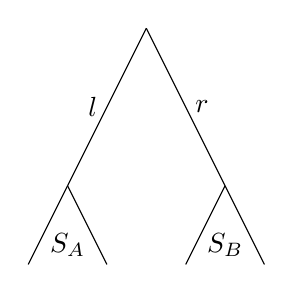
\begin{tikzpicture}
  \coordinate (P) at (0,2);
  \coordinate (A) at (-1.0,0);
  \coordinate (A1) at (-1.5,-1.0);
  \coordinate (A2) at (-0.5,-1.0);
  \coordinate (B) at (1,0);
  \coordinate (B1) at (0.50,-1.0);
  \coordinate (B2) at (1.5,-1.0);
  \node (SA) at (-1.0,-0.75) {$S_A$};
  \node (SB) at (1.0,-0.75) {$S_B$};
  \draw[] (P) -- node [left] {$l$} (A);
  \draw[] (P) -- node [right] {$r$} (B);
  \draw[] (A) -- (A1);
  \draw[] (A) -- (A2);
  \draw[] (B) -- (B1);
  \draw[] (B) -- (B2);
\end{tikzpicture}
\]

(weak coproduct diagram) %FIXME

extends to Weak Biproducts of arbitrary Set-indexed Families of Types
$\bigoplus_{i \in I} A_i$

In Process Calculus, these constructions yield \emph{Disjointly
  Guarded Sums}

Name-free, Names controlled indirectly via Types

applying general definition of Non-determinism and Semi-additivity
obtains $p + q = p \cup q$ which is the Interpretation of
Non-determinism in the Trace Model

in $\cat{ASProc}$ with Processes as Synchronization Trees Modulo Weak
Bisimulation, $p+q$ is a Non-associative version of CSP \emph{Internal
  Choice} $p \sqcap q$


\asterism


\textbf{Input/Output}

Type $X$:
\begin{align*}
  \Sigma_X &= \{\bullet\} \\
  S_X &= \Sigma_X^*
\end{align*}

Type $Y$ for an Input/Output pair Communicating with a single Client:
\begin{align*}
  \Sigma_Y &= \{inl(\bullet), inr(\bullet)\} \\
  S_Y &= a.b.S_Y + ab.S_Y
\end{align*}
where $a$, $b$, and $ab$ are abbreviations for $\{inl(\bullet)\}$,
$\{inr(\bullet)\}$, and $\{inl(\bullet),inr(\bullet)\}$, resp.
Compatible Clients are of the form $a.b.P$ where $P$ is the
Continuation Process.

\interrobang Note the above is inferred from the examples of Clients
given in \cite{abramsky-gay-nagarajan96}: $client = a.b.client$ and
$client = a.b.nil$

$cell : X \parr ... \parr X$

\fist Note unlike in $\cat{SProc}$, the Asynchronous Ports do not need
Delays ($\delta\Delta X$)


\textbf{Safety Specifications}

the above definition of $Y$ for an Input/Output pair Communicating
with a single Client has Deadlock Freedom

Example desired Safety Specification: ``Clients of a Scheduler are
Scheduled Cyclically''

$p : A$

Type $S$ with same Alphabet as $A$ but more restricted Safety
Specification

\emph{Safety Morphism} -- $s: A \rightarrow A$ such that $p : I
\rightarrow A$ Satisfies the Specification in $S$ if and only if $p =
s \circ p$

expresses stronger Specifications without ``forgetting'' what the
Interface looks like

for $s = \id_S$ (considered as a Morphism $A \rightarrow A$ because
$S_S \subseteq S_A$), $p = s \circ p \Leftrightarrow traces(p)
\subseteq S_S$

Correctness Proofs of Processes built from Subcomponents

(scheduler example)



% --------------------------------------------------------------------
\subsection{Proof Net} \label{sec:proof_net}
% --------------------------------------------------------------------

\cite{llwiki16}

Proof Nets can be seen as a Quotient of One-sided Sequent Calculus
Proofs (\S\ref{sec:sequent_calculus}) under Commutation of Rules



% --------------------------------------------------------------------
\subsection{Geometry of Synthesis} \label{sec:geometry_of_synthesis}
% --------------------------------------------------------------------

Bounded version of Geometry of Interaction



% --------------------------------------------------------------------
\subsection{Multiobject GOI}\label{sec:multiobject_goi}
% --------------------------------------------------------------------

\cite{haghverdi-scott05}

Multiplicative Linear Logic (\S\ref{sec:multiplicative_linear_logic})

Parital Trace (\S\ref{sec:partial_trace})



% --------------------------------------------------------------------
\subsection{Linear Combinatory Algebra}\label{sec:linear_combinatory_algebra}
% --------------------------------------------------------------------

2002 - Abramsky-Haghverdi-Scott - \emph{Geometry of Interaction and Linear
  Combinatory Algebras}

used for Realisers in Quantitative Type Theory
(\S\ref{sec:quantitative_type})



% ====================================================================
\section{Calculus of Capabilities}\label{sec:capabilities_calculus}
% ====================================================================

Crary-Walker-Morrisett99 \emph{Typed Memory Management in a Calculus
  of Capabilities}

Region-based Memory Management

Continuation-passing-style Language

Chargueraud-Pottier07 \emph{Functional Translation of a Calculus of
  Capabilities}

Walker-Morrisett00 \emph{Alias Types for Recursive Data Structures}

Alias Types (\S\ref{sec:alias_type})

cf. \emph{Reflective Higher-Order (RHO) Calculus} (\S\ref{sec:rho_calculus});
Namespace Logic (\S\ref{sec:namespace_logic}), Spatial-behavioral Types
(\S\ref{sec:spatial_behavioral})



% --------------------------------------------------------------------
\subsection{Capability}\label{sec:capability}
% --------------------------------------------------------------------

Shi-Xi13 -- Views (\S\ref{sec:view}) can be seen as Linear Types for
classifying Capabilities

cf. Object-Capability Model (Information Security Model), Capability-based
Security

2013 - Meredith, Stay, Drossopoulou - \emph{Policy as Types} -- Hennesy-Milner
Logic (\S\ref{sec:hennesy_milner}); \emph{Deniability} specifications are Open
and describe Necessary Conditions for some Effect to take place; cf. Hoare
Logic specifications describing Sufficient Conditions and are Closed

  \pagebreak[4]%%%%%%%%%%%%%%%%%%%%%%%%%%%%%%%%%%%%%%%%%%%%%%%%%%%%%%%%%%%%%%%%%%%%%%
%%%%%%%%%%%%%%%%%%%%%%%%%%%%%%%%%%%%%%%%%%%%%%%%%%%%%%%%%%%%%%%%%%%%%%
\part{Combinatorics}\label{part:combinatorics}
%%%%%%%%%%%%%%%%%%%%%%%%%%%%%%%%%%%%%%%%%%%%%%%%%%%%%%%%%%%%%%%%%%%%%%
%%%%%%%%%%%%%%%%%%%%%%%%%%%%%%%%%%%%%%%%%%%%%%%%%%%%%%%%%%%%%%%%%%%%%%

Discrete, Countable (\S\ref{sec:countably_infinite})

Abstract Structure (\S\ref{sec:abstract_structure}): Recognizable
Structure vs. Combinatoric description (requiring special arguments)

Formal Language Theory (Part \ref{part:formal_language}):
Combinatorics on Words (\S\ref{sec:combinatorics_on_words})

Enumerative Combinatorics (\S\ref{sec:enumerative_combinatorics}): computing
the number of Elements of \emph{Finite Sets}

Set Theory (Part \ref{part:set_theory}): Infinitary Combinitorics
(\S\ref{sec:infinitary_combinatorics}) \fist Cardinality
(\S\ref{sec:cardinality})

\fist Discrete Geometry (Combinatorial Geometry \S\ref{sec:discrete_geometry})

\fist Discrete Uniform Law (Probability Theory \S\ref{sec:discrete_uniform})



% ====================================================================
\section{Combination}\label{sec:combination}
% ====================================================================

Unordered choice of Elements

$k$-combination of $n$ Elements is given by the Binomial Coefficient
(\S\ref{sec:binomial_coefficient}) $\binom{n}{k}$, $n$ ``choose'' $k$,
equal to:
\[
  \frac{n!}{k!(n - k)!}
\]



% --------------------------------------------------------------------
\subsection{Binomial Coefficient}\label{sec:binomial_coefficient}
% --------------------------------------------------------------------

Binomial (\S\ref{sec:binomial})

$\binom{n}{k} = \frac{n!}{k!(n - k)!}$

number of ways to Partition a Set of Cardinality $n$ into two Subsets of
Cardinality $k$ and $n-k$

counting Partitions (\S\ref{sec:partition}) of prescribed Cardinalities:

$\binom{n}{n_1 n_2 \cdots n_k}$



% ====================================================================
\section{Permutation}\label{sec:permutation}
% ====================================================================

Ordered choice of Elements

The number of Permutations of $n$ Elements is $n!$

The number of Cyclic Permutations (\S\ref{sec:cyclic_permutation}) of
$n$ Elements is $(n-1)!$

The number of $k$ choices out of $n$ Elements when order is
significant is $\frac{n!}{(n-1)!}$

Permutation Group (\S\ref{sec:permutation_group})



% --------------------------------------------------------------------
\subsection{Cyclic Permutation}\label{sec:cyclic_permutation}
% --------------------------------------------------------------------

A Permutation is \emph{Cyclic} if and only if it consists of a single
Non-trivial Cycle (Cycle Length > 1).



\subsubsection{Transposition}\label{sec:transposition}

A \emph{Transposition} is a Cyclic Permutation of length 2 which
exchanges two Elements and leaves all other Elements fixed.



% --------------------------------------------------------------------
\subsection{Derangement}\label{sec:derangement}
% --------------------------------------------------------------------

a Permutation such that no Element appears in its original position, i.e. a
Permutation with no \emph{Fixed Points}



% ====================================================================
\section{Partition}\label{sec:partition}
% ====================================================================

Set Partitions (\S\ref{sec:set_partition})

Binomial Coefficient (\S\ref{sec:binomial_coefficient})

$\binom{n}{n_1 n_2 \cdots n_k}$



% --------------------------------------------------------------------
\subsection{Bell Number}\label{sec:bell_number}
% --------------------------------------------------------------------

Bell Number

$B_{n+1} = \sum_{k=0}^n \binom{n}{k} B_k$



% ====================================================================
\section{Transversal}\label{sec:transversal}
% ====================================================================

% ====================================================================
\section{Enumerative Combinatorics}
\label{sec:enumerative_combinatorics}
% ====================================================================

Counting Structures



% --------------------------------------------------------------------
\subsection{The Twelvefold Way}\label{sec:twelvefold_way}
% --------------------------------------------------------------------

(wiki):

Systematic classification of 12 related Enumerative problems concerning two
Finite Sets, including classical problems of counting:
\begin{itemize}
  \item Permutations (\S\ref{sec:permutation})
  \item Combinations (\S\ref{sec:combination})
  \item Multisets (\S\ref{sec:multiset})
  \item Partitions of a Set (\S\ref{sec:partition})
  \item Partitions of an Integer (\S\ref{sec:integer_partition})
\end{itemize}

Cases:
\begin{enumerate}
  \item Functions from $N$ to $X$
  \item Functions from $N$ to $X$, up to a Permutation of $N$
  \item Functions from $N$ to $X$, up to a Permutation of $X$
  \item Functions from $N$ to $X$, up to Permutations of $N$ and $X$
  \item Injective Functions from $N$ to $X$
  \item Injective Functions from $N$ to $X$, up to a Permutation of $N$
  \item Injective Functions from $N$ to $X$, up to a Permutation of $X$
  \item Injective Functions from $N$ to $X$, up to Permutations of $N$ and $X$
  \item Surjective Functions from $N$ to $X$
  \item Surjective Functions from $N$ to $X$, up to a Permutation of $N$
  \item Surjective Functions from $N$ to $X$, up to a Permutation of $X$
  \item Surjective Functions from $N$ to $X$, up to Permutations of $N$ and $X$
\end{enumerate}



% --------------------------------------------------------------------
\subsection{Lattice Path}\label{sec:lattice_path}
% --------------------------------------------------------------------

\subsubsection{Dyck Path}\label{sec:dyck_path}

\subsubsection{Schr\"oder Path}\label{sec:schroder_path}

\emph{Schr\"oder Paths and Reverse Bessel Polynomials} --
\url{https://golem.ph.utexas.edu/category/2017/08/schrder_paths_and_reverse_bessel_polynomials.html}

Reverse Bessel Polynomial (\S\ref{sec:reverse_bessel_polynomial})



% ====================================================================
\section{Analytic Combinatorics}\label{sec:analytic_combinatorics}
\cite{flajolet-sedgewick09}
% ====================================================================

Asymptotic Analysis (\S\ref{sec:asymptotic_analysis})



% --------------------------------------------------------------------
\subsection{Combinatorial Species}\label{sec:combinatorial_species}
% --------------------------------------------------------------------



% ====================================================================
\section{Design Theory}\label{sec:combinatorial_design}
% ====================================================================

% ====================================================================
\section{Algebraic Combinatorics}\label{sec:algebraic_combinatorics}
% ====================================================================

% --------------------------------------------------------------------
\subsection{Polynomial Sequence}\label{sec:polynomial_sequence}
% --------------------------------------------------------------------

Polynomial (\S\ref{sec:polynomial}) Sequence (\S\ref{sec:sequence})



\subsubsection{Orthogonal Polynomial Sequence}
\label{sec:orthogonal_polynomial_sequence}

\paragraph{Bessel Polynomial}\label{sec:bessel_polynomial}\hfill

\subparagraph{Reverse Bessel Polynomial}\label{sec:reverse_bessel_polynomial}
\hfill

cf. Bessel Functions (\S\ref{sec:bessel_function})

\emph{Schr\"oder Paths and Reverse Bessel Polynomials} --
\url{https://golem.ph.utexas.edu/category/2017/08/schrder_paths_and_reverse_bessel_polynomials.html}

Schr\"oder Path (\S\ref{sec:schroder_path})



% --------------------------------------------------------------------
\subsection{Matroid Theory}\label{sec:matroid_theory}
% --------------------------------------------------------------------

\subsubsection{Matroid}\label{sec:matroid}

\subsubsection{Antimatroid}\label{sec:antimatroid}

\subsubsection{Greedoid}\label{sec:greedoid}



% ====================================================================
\section{Extremal Combinatorics}\label{sec:extremal_combinatorics}
% ====================================================================

Combinatorial Optimization (\S\ref{sec:combinatorial_optimization})



% --------------------------------------------------------------------
\subsection{Ramsey Theory}\label{sec:ramsey_theory}
% --------------------------------------------------------------------

\subsubsection{Ramsey's Theorem}\label{sec:ramseys_theorem}



% ====================================================================
\section{Probabilistic Combinatorics}\label{sec:probabilistic_combinatorics}
% ====================================================================

Probability Theory (Part \S\ref{part:probability_theory})



% --------------------------------------------------------------------
\subsection{Probabilistic Method}\label{sec:probabilistic_method}
% --------------------------------------------------------------------



% ====================================================================
\section{Infinitary Combinatorics}\label{sec:infinitary_combinatorics}
% ====================================================================

Set Theory (Part \ref{part:set_theory})

\emph{Combinatorial Set Theory}

Graphons (``Continuous Graphs'' \S\ref{sec:graphon})



% ====================================================================
\section{Combinatorics on Words}\label{sec:combinatorics_on_words}
% ====================================================================

Formal Language Theory (Part \ref{part:formal_language})

Chomasky Hierarchy (\S\ref{sec:chomsky_hierarchy})



% --------------------------------------------------------------------
\subsection{Word Type}\label{sec:word_type}
% --------------------------------------------------------------------

\subsubsection{Sturmian Word}\label{sec:sturmian_word}

\subsubsection{Lyndon Word}\label{sec:lyndon_word}



% ====================================================================
\section{Combinatory Logic}\label{sec:combinatory_logic}
% ====================================================================

*FIXME*: this section probably doesn't belong under ``Combinatorics'', move to
type theory or recursion theory ???

Higher-order Functions (\S\ref{sec:higherorder_function})

\fist cf. Predicate Functor Logic (\S\ref{sec:pfl})

Set Theory (Part \S\ref{part:set_theory})

Combinatory Logic may be given as a variant of $\lambda$-calculus
(\S\ref{sec:untyped_lambda}) where Lambda Expressions are replaced by
\emph{Combinators} (\S\ref{sec:combinator}) which are Primitive
Functions witout Bound Variables ($\lambda$-calculus without
Abstraction).

SKI Combinator Calculus (\S\ref{sec:ski_calculus})

$\lambda$-terms can be transformed into Combinatory Logic by
Abstraction Elimination (\S\ref{sec:abstraction_elimination})

It is Undecidable whether a given Combinatory Term has a Normal Form
(or whether two Combinatory Terms are Equivalent).

By the Curry-Howard Correspondence (\S\ref{sec:curry_howard}) a Typed
Combinatory Logic corresponds to a Hilbert System
(\S\ref{sec:hilbert_system}) in Proof Theory.



% --------------------------------------------------------------------
\subsection{Combinator}\label{sec:combinator}
% --------------------------------------------------------------------

\emph{Combinator} (or \emph{Constant})

Closed Primitive Function

Identity:
\[
  I x = x
\]
Constant:
\[
  K x y = x
\]
Application (Sequence):
\[
  S x y z = x z (y z)
\]

Identity may be defined in Terms of $S$ and $K$:
\[
  (S K K) x = I x
\]

$\Omega$-combinator: $(\lambda x. x x)$



\subsubsection{Fixed-point Combinator}\label{sec:fixedpoint_combinator}

\[
  y f = f (y f)
\]
represents a Solution to the Fixed Point Equation
(\S\ref{sec:fixed_point}):
\[
  x = f x
\]



\paragraph{$Y$-combinator}\label{sec:y_combinator}\hfill

In Simply-typed $\lambda$-calculus, the $Y$-combinator cannot be
assigned a Type.

\[
  Y = \lambda f.(\lambda x.f (x x)) (\lambda x.f (x x))
\]

Allows for \emph{Anonymous Recursion} in Programming Languages.
%FIXME xref?



\subsubsection{Non-standard Fixed-point Combinator}
\label{sec:nonstandard_combinator}

A \emph{Non-standard Fixed-point Combinator} is a Combinator that has
the same Infinite Extension (B\"ohm Tree \S\ref{sec:bohm_tree}) as a
Fixed-point Combinator. Every Fixed-point Combinator is a Non-standard
Fixed-point Combinator, but not every Non-standard Fixed-point
Combinator is a Fixed-point Combinator. A Non-standard Fixed-point
Combinator that is not a Fixed-point Combinator is called a
\emph{Strictly Non-standard Fixed-point Combinator}.

The Set of Non-standard Fixed-point Combinators is not Recursively
Enumerable. \cite{goldberg05}



% --------------------------------------------------------------------
\subsection{Combinatory Term}\label{sec:combinatory_term}
% --------------------------------------------------------------------

Curry \emph{Theory of Functionality}

\begin{itemize}
  \item a Variable $x$
  \item a Combinator (Constant) $P$
  \item Application of Combinatory Terms $E_1 E_2$
\end{itemize}
Variables and Constants are \emph{Atoms}.



\subsubsection{Contraction}\label{sec:combinatory_contraction}
\cite{seldin03}

Basic Combinators:
\begin{enumerate}
  \item $\mathsf{I} X = X$
  \item $\mathsf{K} X Y = X$
  \item $\mathsf{S} X Y Z = (X Z) (Y Z)$
\end{enumerate}

Weak Reduction, a Sequence of Zero or more Contractions: $M \rhd N$

Weak Conversion, a Sequence of Zero or more Contractions and reverse
Contractions: $M =_* N$



\subsubsection{Bracket Abstraction}\label{sec:bracket_abstraction}

\emph{Abstraction} of Term $M$ with respect to Variable $x$ denoted
$[x]M$, defined Inductively:\cite{seldin03}
\[
  [x]x \equiv \mathsf{I}
\]\[
  [x]c \equiv \mathsf{K}c
\]\[
  [x](M N) \equiv \mathsf{S}([x]M)([x]N)
\]
where $c$ is an Atom other than $x$ and $\equiv$ is an Equivalence of
Terms.

Theorem:
\[
  ([x]M)N \rhd [N/x]M
\]



\subsubsection{Abstraction Elimination}
\label{sec:abstraction_elimination}



\subsubsection{Type Assignment}\label{sec:combinatory_type}
\cite{seldin03}

\begin{itemize}
  \item ($\rightarrow \mathsf{I}$) $\mathsf{I}: A \rightarrow A$
  \item ($\rightarrow \mathsf{K}$)
    $\mathsf{K}: A \rightarrow (B \rightarrow A)$
  \item ($\rightarrow \mathsf{S}$)
    $\mathsf{S}: (A \rightarrow (B \rightarrow C))
      \rightarrow (A \rightarrow B) \rightarrow A \rightarrow C$
\end{itemize}

Derived Rule (cf. Modus Ponens):
\[
  \frac{
    [x:A] \quad m:B
  }{
    [x]m:A \rightarrow B
  }
\]



% --------------------------------------------------------------------
\subsection{BCI Combinatory Logic}\label{sec:bci_logic}
% --------------------------------------------------------------------

Linear Logic (\S\ref{sec:linear_logic})

Combinators have the Types of the basic Operations in a Symmetric
Closed Category (\S\ref{sec:symmetric_closed_category})


% --------------------------------------------------------------------
\subsection{BCK Combinatory Logic}\label{sec:bck_logic}
% --------------------------------------------------------------------

Affine Logic (\S\ref{sec:affine_logic})



% ====================================================================
\section{Arithmetic Combinatorics}\label{sec:arithmetic_combinatorics}
% ====================================================================

Ergodic Ramsey Theory

  \pagebreak[4]%%%%%%%%%%%%%%%%%%%%%%%%%%%%%%%%%%%%%%%%%%%%%%%%%%%%%%%%%%%%%%%%%%%%%%
%%%%%%%%%%%%%%%%%%%%%%%%%%%%%%%%%%%%%%%%%%%%%%%%%%%%%%%%%%%%%%%%%%%%%%
\part{Type Theory}\label{sec:type_theory}
%%%%%%%%%%%%%%%%%%%%%%%%%%%%%%%%%%%%%%%%%%%%%%%%%%%%%%%%%%%%%%%%%%%%%%
%%%%%%%%%%%%%%%%%%%%%%%%%%%%%%%%%%%%%%%%%%%%%%%%%%%%%%%%%%%%%%%%%%%%%%

\emph{Type Theory} is the study of classes of Formal Systems
(\S\ref{sec:formal_system}) where each Term
(\S\ref{sec:term}) has a \emph{Type} and Operations
are restricted to Terms of specific Types.

As a Formal Theory (Part \ref{sec:proof_theory}), Judgements in Type
Theory are of three kinds\cite{hott13}:
\begin{enumerate}

\item \emph{Well-formed Context} (\S\ref{sec:type_context})
\[
    (\Gamma) ctx
\]
``$\Gamma$ is a Well-formed Context''

\item \emph{Propositional Equality}
\[
    \Gamma \vdash a : A
\]
``Given Contex $\Gamma$, $a$ is a Term of Type $A$''

\item \emph{Definitional (Judgemental) Equality}
\[
    \Gamma \vdash a \equiv b : A
\]
``Given Context $\Gamma$, $a$ and $b$ are definitionally equal Terms
of Type $A$''

\end{enumerate}
with a Deductive Apparatus (\S\ref{sec:deductive_apparatus})
consisting of Inference Rules only and no Axioms. Judgemental Equality
is an Equivalence Relation respected by Typing.

Inference Rules have the form:
\[
    \frac{J_1 \quad \cdots \quad J_k} {J} Name
\]
where $J_i$ are provided as derived hypothetical (metatheoretical)
Judgements and $J$ is the conclusion.

A tree constructed from Inference Rules forms a \emph{Derivation} of a
Judgement.



% ====================================================================
\section{Expression}\label{sec:type_expression}
% ====================================================================

An \emph{Expression} is an Equivalence Class of Syntactic forms which
differ in the names of \emph{Bound Variables}. That is, changing the
name of a Bound Variable everywhere within an Expression
(\emph{$\alpha$-conversion}) does not change the Expression.

A Variable is Bound in an Expression by an \emph{Abstraction}
expressing that the Variable is \emph{local} to the Expression:
\[
    \lambda x.B
\]
or
\[
    x.B
\]

\emph{Substitution}:
\[
    B[a/x]
\]
Substitute Term $a$ for Free occurrences of Variable $x$ in the Term
$B$. Generalized:
\[
    B[a_1,\ldots,a_n / x_1,\ldots,x_n]
\]



% ====================================================================
\section{Context}\label{sec:type_context}
% ====================================================================

A \emph{Context}, $\Gamma$, is a list of Assumptions of the form:
\[
    \Gamma = x_1 : A_1, x_2 : A_2, \ldots, x_n : A_n
\]
where each Element $x_i : A_i$ is an Assumption that the distinct
Variable $x_i$ has type $A_i$.

Judgements are formulated under the Assumptions of a particular
Context, $\Gamma$:
\[
    \Gamma \vdash a : A
\]
For an empty Context:
\[
    \vdash a : A
\]
or
\[
    . \vdash a : A
\]



% ====================================================================
\section{Type}\label{sec:type}
% ====================================================================

% --------------------------------------------------------------------
\subsection{Ramified Type}\label{sec:ramified_type}
% --------------------------------------------------------------------



% ====================================================================
\section{Type Universe}\label{sec:type_universe}
% ====================================================================

A \emph{Type Universe} is a Type whose Elements are Types. A hierarchy:
\[
    \mathcal{U}_0, \mathcal{U}_1, \mathcal{U}_2, \ldots
\]
is such that any Type in $\mathcal{U}_i$ is also in
$\mathcal{U}_{i+1}$. See $\mathcal{U}-INTRO$ and $\mathcal{U}-CUMUL$
\S\ref{sec:universe_rules}.



% ====================================================================
\section{Inference Rules}\label{sec:type_inference}
% ====================================================================

% --------------------------------------------------------------------
\subsection{Context Rules}
% --------------------------------------------------------------------

The following Rules of Inference allow for the determination of a
Well-formed Context:
\begin{enumerate}
\item
\[
    {
        \frac{}{(.)ctx}
    } ctx-EMP
\]
\item
\[
    {
        \frac
        {x_1:A_1, \ldots, x_{n-1}:A_{n-1} \vdash A_n : \mathcal{U}_i}
        {(x_1:A_1,\ldots,x_n:A_n) ctx}
    } ctx-EXT
\]
\end{enumerate}



% --------------------------------------------------------------------
\subsection{Structural Rules}
% --------------------------------------------------------------------

Given a Context, derive Typing Judgements listed in the Context:
\[
    {
        \frac
        {(x_1:A_1, \ldots, x_n:A_n)ctx}
        {x_1:A_1, \ldots, x_n:A_n \vdash x_i:A_i}
    } Vble
\]

Substitution for Typing Judgements:
\[
    {
        \frac
        {\Gamma \vdash a : A \;\;\;\;\;\;\;
        \Gamma,x:A,\Delta \vdash b : B}
        {\Gamma,\Delta[a/x] \vdash b[a/x] : B[a/x]}
    } Subst_1
\]

Weakening for Typing Judgements:
\[
    {
        \frac
        {\Gamma \vdash A : \mathcal{U}_i \;\;\;\;\;\;\;
        \Gamma,\Delta \vdash b : B}
        {\Gamma,x:A,\Delta \vdash b:B}
    } Wkg_1
\]

Substitution for Judgemental Equality:
\[
    {
        \frac
        {\Gamma \vdash a : A \;\;\;\;\;\;\;
        \Gamma,x:A,\Delta \vdash b \equiv c : B}
        {\Gamma,\Delta[a/x] \vdash b[a/x] \equiv c[a/x] : B[a/x]}
    } Subst_2
\]

Weakening for Judgemental Equality:
\[
    {
        \frac
        {\Gamma \vdash A : \mathcal{U}_i \;\;\;\;\;\;\;
        \Gamma,\Delta \vdash b \equiv c : B}
        {\Gamma, x:A, \Delta \vdash b \equiv c : B}
    } Wkg_2
\]



% --------------------------------------------------------------------
\subsection{Universe Rules}\label{sec:universe_rules}
% --------------------------------------------------------------------

\[
    {
        \frac
        {(\Gamma) ctx}
        {\Gamma \vdash \mathcal{U}_i : \mathcal{U}_{i+1}}
    } \mathcal{U}-INTRO
\]

\[
    {
        \frac
        {\Gamma \vdash A : \mathcal{U}_i}
        {\Gamma \vdash A : \mathcal{U}_{i+1}}
    } \mathcal{U}-CUMUL
\]



% --------------------------------------------------------------------
\subsection{Dependent Function Type Rules}\label{sec:dependent_rules}
% --------------------------------------------------------------------

\[
    {
        \frac
        {\Gamma \vdash A : \mathcal{U}_i \;\;\;\;\;\;\;
        \Gamma,x:A \vdash B : \mathcal{U}_i}
        {\Gamma \vdash \prod_{(x:A)} B : \mathcal{U}_i}
    } \Pi-FORM
\]\[
    {
        \frac
        {}
        {}
    } \Pi-INTRO
\]\[
    {
        \frac
        {}
        {}
    } \Pi-ELIM
\]\[
    {
        \frac
        {}
        {}
    } \Pi-COMP
\]\[
    {
        \frac
        {}
        {}
    } \Pi-UNIQ
\]



% ====================================================================
\section{Typed $\lambda$-Calculus}\label{sec:typed_lambda}
% ====================================================================

% --------------------------------------------------------------------
\subsection{Simply Typed $\lambda$-Calculus}\label{sec:simply_typed}
% --------------------------------------------------------------------

Isomorphic by Curry-Howard (\S\ref{sec:curry_howard}) to
Propositional Logic (\S\ref{sec:propositional_logic})

Propositional Logic $\leftrightarrow$ Simply Typed $\lambda$-Calculus:
\[
    \supset \leftrightarrow \rightarrow
\] \[
    \wedge \leftrightarrow \times
\] \[
    \vee \leftrightarrow +
\] \[
    False \leftrightarrow \bot
\]



% --------------------------------------------------------------------
\subsection{Second-order $\lambda$-Calculus}
\label{sec:secondorder_lambda_calculus}
% --------------------------------------------------------------------



% --------------------------------------------------------------------
\subsection{Calculus of Constructions}\label{sec:coq}
% --------------------------------------------------------------------



% ====================================================================
\section{Intuitionistic Type Theory}\label{sec:intuitionistic_type}
% ====================================================================

\emph{Intuitionistic Type Theory} (also \emph{Constructive Type
  Theory} or \emph{Martin-L\"of Type Theory})

Inductive Types



% --------------------------------------------------------------------
\subsection{Types}
% --------------------------------------------------------------------

\emph{Function Type}

\emph{Higher-order Function}

\emph{Product Type}

\subsubsection{Empty Type $\mathbf{0}$}

\subsubsection{Unit Type $\mathbf{1}$}

\subsubsection{Natural Number Type}

\subsubsection{Identity Type}

\subsubsection{Dependent Function Type ($\Pi$-type)}

\[
    A \rightarrow B :\equiv \prod_{x:A} B
\]

\subsubsection{Dependent Pair Type ($\Sigma$-type)}

In Set Theory: Indexed Sum over a given Type.

\subsubsection{Coproduct Type}



% --------------------------------------------------------------------
\subsection{Intensional \& Extensional Type Theory}
\label{sec:intension_extension}
% --------------------------------------------------------------------

\emph{Canonical Form}

\emph{Normal Form}



% ====================================================================
\section{Pure Type System}\label{sec:pure_type_sytem}
% ====================================================================

Arbitrary number of Sorts and Dependencies

Generalization of the \emph{Lambda Cube} to more sorts than Terms and
Types

Not necessarily Strongly Normalizing (\S\ref{sec:normalization})



% --------------------------------------------------------------------
\subsection{Lambda Cube}\label{sec:lambda_cube}
% --------------------------------------------------------------------

Simply-typed $\lambda$-calculus allows only Terms to depend on Types.



% --------------------------------------------------------------------
\subsection{Subtype}\label{sec:subtype}
% --------------------------------------------------------------------



% ====================================================================
\section{Homotopy Type Theory}\label{sec:homotopy_type}
% ====================================================================

- Function Extensionality
- Univalence Axiom
- Higher Inductive Types



% ====================================================================
\section{Curry-Howard Correspondence}\label{sec:curry_howard}
% ====================================================================

\begin{tabular}{| l | l |}
\hline
\textbf{Type Theory} & \textbf{Logic} \\ \hline \hline
$A$ (Type) & Proposition \\ \hline
$a : A$ (Term) & Proof \\
\hline
\end{tabular}

Natural Deduction - Typed Lambda Calculus

Propositional Logic - Simple Types

Predicate Logic - Dependent Types

Modal Logic - Monads

Classical-Intuitionistic Embedding - Continuation Passing Style



% ====================================================================
\section{Type System}\label{sec:type_system}
% ====================================================================

% --------------------------------------------------------------------
\subsection{Hindley-Milner Type System}\label{sec:hindley_milner}
% --------------------------------------------------------------------

  \pagebreak[4]%%%%%%%%%%%%%%%%%%%%%%%%%%%%%%%%%%%%%%%%%%%%%%%%%%%%%%%%%%%%%%%%%%%%%%%%%%%%%%%%
%%%%%%%%%%%%%%%%%%%%%%%%%%%%%%%%%%%%%%%%%%%%%%%%%%%%%%%%%%%%%%%%%%%%%%%%%%%%%%%%
\part{Database Theory}\label{part:database_theory}
%%%%%%%%%%%%%%%%%%%%%%%%%%%%%%%%%%%%%%%%%%%%%%%%%%%%%%%%%%%%%%%%%%%%%%%%%%%%%%%%
%%%%%%%%%%%%%%%%%%%%%%%%%%%%%%%%%%%%%%%%%%%%%%%%%%%%%%%%%%%%%%%%%%%%%%%%%%%%%%%%

% ==============================================================================
\section{Data}\label{sec:data}
% ==============================================================================

\emph{Sample Data} (\emph{Statistical Sample} \S\ref{sec:sample})

when viewed ``in context'', Data conveys \emph{Information}
(\S\ref{sec:information})

\fist cf. Datatype (Type Theory \S\ref{sec:datatype}), Statistical Data Type
(\S\ref{sec:statistical_data_type})



% ------------------------------------------------------------------------------
\subsection{Data Item}\label{sec:data_item}
% ------------------------------------------------------------------------------

cf. ``\emph{Data Point}'' (Statistical Sample \S\ref{sec:sample})



% ------------------------------------------------------------------------------
\subsection{Data Collection}\label{sec:data_collection}
% ------------------------------------------------------------------------------

cf. \emph{Data Generating Process} (\S\ref{sec:data_generating_process}),
\emph{Sampling} (\S\ref{sec:sampling})



% ------------------------------------------------------------------------------
\subsection{Dataset}\label{sec:dataset}
% ------------------------------------------------------------------------------

cf. \emph{Sample Data} (\emph{Statistical Sample} \S\ref{sec:sample})

\fist Statistical Transformations (\S\ref{sec:dataset_transformation}) of
Datasets

Datasets in Machine Learning Algorithms (\S\ref{sec:learning_algorithm}):
\begin{itemize}
  \item Training Dataset (\S\ref{sec:training_dataset})
  \item Validation Dataset (\S\ref{sec:validation_dataset})
  \item Test Dataset (\S\ref{sec:test_dataset})
\end{itemize}



% ==============================================================================
\section{Data Structure}\label{sec:data_structure}
% ==============================================================================

%FIXME possibly move this section?

potentially Infinite Data Structures: Abstracted as $F$-coalgebras
(\S\ref{sec:f_coalgebra})

(also Data Structure as Folds of Church Encodings)
%??? FIXME

(Milewski - Understanding F-Algebras)

As Recursive Functions are defined as Fixed Points of regular
Functions, (Nested) Data Structures can be defined as Fixed Points of
regular Type Constructors.

Functors as Type Constructors give rise to Nested Data Structures that
allow Recursive Evaluation (generalized Folding).

2002 - Giavitto, Michel - \emph{Data Structure as Topological Spaces}:

a Data Structure $s$ is an ``\emph{Organization}'' $o$ performed on a Dataset
$D$: $s = (o, D)$, e.g. $s = (list, int)$



% -----------------------------------------------------------------------------
\subsection{Ordered Tree}\label{sec:ordered_tree}
% -----------------------------------------------------------------------------

\subsubsection{Trie}\label{sec:trie}

\subsubsection{Prefix Tree}\label{sec:prefix_tree}

\subsubsection{Suffix Tree}\label{sec:suffix_tree}



% -----------------------------------------------------------------------------
\subsection{Fingertree}\label{sec:fingertree}
% -----------------------------------------------------------------------------



% ==============================================================================
\section{Data Transformation}\label{sec:data_transformation}
% ==============================================================================

\fist cf. Statistical Data Transformation (\S\ref{sec:dataset_transformation})



% -----------------------------------------------------------------------------
\subsection{Bidirectional Transformation}
\label{sec:bidirectional_transformation}
% -----------------------------------------------------------------------------

\subsubsection{Bidirectional Model Tranformation}
\label{sec:bidirectional_model_transformation}

\subsubsection{Optic}\label{sec:optic}

%FIXME: move to category theory ???

\url{https://golem.ph.utexas.edu/category/2020/01/profunctor_optics_the_categori.html}

compositional representation of \emph{Bidirectional Data Accessors}

originally called \emph{Accessors} or \emph{Generalized Functional References}

\emph{Profunctor Encoding} -- \emph{Profunctor Optics}
(\S\ref{sec:profunctor_optics})

\emph{van Laarhoven Encoding} -- Haskell $\mathtt{lens}$ library

%FIXME: move to profunctor subsection ?

\url{https://julesh.com/2023/01/28/geometry-of-interaction-is-the-optic-for-copointed-functors/}
-- Geometry of Interaction (\S\ref{sec:interaction_geometry}) is the Optic for
Co-pointed Functors

\url{https://ncatlab.org/nlab/show/optic+%28in+computer+science%29}

\url{http://oleg.fi/gists/posts/2017-04-18-glassery.html}

\url{https://golem.ph.utexas.edu/category/2020/01/profunctor_optics_the_categori.html}

compositional representation of \emph{Bidirectional Data Accessors}

\emph{Lens} (\S\ref{sec:lens}) -- Products; \emph{Note}: not the same as
``Lenses'' (Anamorphism or \emph{Co-iteration} \S\ref{sec:anamorphism}) in
Recursion Theory

\emph{view}, \emph{update}

``Generalized Functional References''

\emph{Prism} -- Tagged Unions; Lenses in the \emph{Opposite} Category

\emph{match}, \emph{build}

\emph{Traversal} -- Containers

\emph{extract}

\emph{Setter}

\emph{Grate}

2018 - Riley - \emph{Categories of Optics}

$\mathbf{Optic} : \mathbf{SymmMonCat} \rightarrow \mathbf{SymmMonCat}$

for a Symmetric Monoidal Category $(\cat{C}, \otimes, I)$, given two Pairs of
Objects of $\cat{C}$, $(S, S')$ and $(A, A')$, an \emph{Optic}
$p : (S, S') \nrightarrow (A, A')$ is an Element of the Set:
\[
  \mathbf{Optic}_\cat{C} ((S, S'), (A, A')) \defeq
    \int^{M\in\cat{C}} \cat{C}(S, M \otimes A) \times \cat{C}(M \otimes A', S')
\]

(Coend Calculus \S\ref{sec:coend})

\asterism

\url{https://www.youtube.com/watch?v=1NHBexWYgkU}

an Optic is given by a choice of a Residual Object $M \in \cat{C}$, a Forward
Map $f$ and a Backward Map $b$

when $\cat{C}$ is Cartesian,
$\mathbf{Optic}(\cat{C}) \simeq \mathbf{Lens}(\cat{C})$



\paragraph{Parametric Optics}\label{sec:parametric_optics}\hfill

\url{https://www.youtube.com/watch?v=1NHBexWYgkU} -- common structure behind
Neural Networks, Loss Functions, and Optimizers

nlab: Para Construction (\S\ref{sec:para_construction}) $Para(Optic(C))$
recovers the Category of Neural Networks (Capucci et al. 2020)



\paragraph{Lens}\label{sec:lens}\hfill

2007 - Foster et al. - \emph{Combinators for bidirectional tree transformations:
A linguistic approach to the view-update problem}

2012 - Johnson et al. - \emph{Lenses, fibrations, and universal translations}

nlab: ``well-behaved'' Lenses are equivalently Co-algebras of the Co-state
Co-monad (O'Connor 2010, 2011)

\fist cf. System T (\S\ref{sec:system_t}) -- Proof Interpretation of Heyting
Arithmetic (\S\ref{sec:heyting_arithmetic}) into a Finite-type Extension of
Primitive Recursive Arithmetic (\S\ref{sec:primitive_recursive}); the
Interpretation of Intuitionistic Implication is the first example of a ``Lense''
from Programming: a Proof of $\varphi \rightarrow \psi$ is a \emph{Lens} from
Proofs of $\varphi$ to Proofs of $\psi$
(\url{https://julesh.com/2018/08/16/lenses-for-philosophers/})

\fist cf. van Laarhoven Free Monad (\S\ref{sec:vanlaarhoven_free_monad}) -- van
Laarhoven Function: $(X \rightarrow F X) \rightarrow F Y$ equivalent to Store
Comonad

Lenses in Compositional Game Theory (Ghani, Hedges 2018)

2021 - Cruttwell et al. - \emph{Categorical Foundations of Gradient-based
Learning} -- Category of Lenses in a Cartesian Category
(\S\ref{sec:cartesian_category}) $\cat{C}$: $\mathbf{Lens}(\cat{C})$



\subparagraph{Asymmetric Lens}\label{sec:asymmetric_lens}\hfill

\subparagraph{Symmetric Lens}\label{sec:symmetric_lens}\hfill

2019 - Fong, Johnson - \emph{Functorial Backpropagation and Symmetric Lenses} -
\url{https://www.youtube.com/watch?v=s0WTRHe-4ZI} -- ``Lenses are Learners'';
\fist Backpropagation (\S\ref{sec:backpropagation})



\subparagraph{Parametric Lens}\label{sec:parametric_lens}\hfill

%FIXME: type of symmetric lens ?

nlab: Para Construction (\S\ref{sec:para_construction}) $Para(Optic(C))$
recovers the Category of Neural Networks (Capucci et al. 2020)

2021 - Cruttwell et al. - \emph{Categorical Foundations of Gradient-based
Learning}

fundamental Semantic structure of Learning (\S\ref{sec:machine_learning});
Parametric Lenses are Open Systems (\S\ref{sec:open_system}) which may be
composed

a Parametric Lens is a ``\emph{Process}'' with three kinds of ``Interfaces'':
Inputs, Outputs, and Parameters, and on each Interface, information flows both
ways, i.e. ``computations'' are bi-directional



\subparagraph{Bare Lens}\label{sec:bare_lens}\hfill

or \emph{Set-based Lens}



\subparagraph{Constant Complement Lens}
\label{sec:constant_complement_lens}\hfill



% ==============================================================================
\section{Data Analysis}\label{sec:data_analysis}
% ==============================================================================

% -----------------------------------------------------------------------------
\subsection{Descriptive Analytics}\label{sec:descriptive_analytics}
% -----------------------------------------------------------------------------

\fist Unsupervised Learning (Cluster Analysis \S\ref{sec:cluster_analysis})



% -----------------------------------------------------------------------------
\subsection{Predictive Analytics}\label{sec:predictive_analytics}
% -----------------------------------------------------------------------------

Predictive Inference (\S\ref{sec:predictive_inference}), Predictive Modeling
(\S\ref{sec:predictive_modeling})

\fist Supervised Learning (Statistical Classification
\S\ref{sec:statistical_classification}, Regression Analysis
\S\ref{sec:regression_analysis})

Time-series Models (\S\ref{sec:time_series_analysis})

cf. Scenario Analysis (\S\ref{sec:scenario_analysis}): based on
\emph{hypothetical} Data, not historical Data



% -----------------------------------------------------------------------------
\subsection{Prescriptive Analytics}\label{sec:prescriptive_analytics}
% -----------------------------------------------------------------------------

- \url{http://www.argmin.net/2018/01/29/taxonomy/} -- Reinforcement Learning
(\S\ref{sec:reinforcement_learning}) as Prescriptive Analytics

\fist Optimal Control (\S\ref{sec:optimal_control})



% ==============================================================================
\section{Relational Algebra}\label{sec:relational_algebra}
% ==============================================================================

\emph{Domain Relational Calculus}



% -----------------------------------------------------------------------------
\subsection{Projection}\label{sec:relational_projection}
% -----------------------------------------------------------------------------



% ==============================================================================
\section{Relational Model}\label{sec:relational_model}
% ==============================================================================

\emph{Relational Calculus}

%FIXME:

2016 - Gibbons - \emph{Comprehending Ringads} -- ``Ringad Comprehensions
represent a convenient notation for expressing \emph{Database Queries}.''



% -----------------------------------------------------------------------------
\subsection{Relation}\label{sec:database_relation}
% -----------------------------------------------------------------------------

(wiki):

A \emph{Relation} is a Heading (\S\ref{sec:heading}) paired with a Body
(\S\ref{sec:body}).

A Relation is a Set of Tuples $(d_1, d_2, \ldots, d_n)$ where each Element $d_j
\in D_j$ is a Member of a Data Domain $D_j$. Unlike a Set Theoretic Relation
(\S\ref{sec:relation}), there is no ordering to the Elements of the Tuples of a
Relation-- each element is called an \emph{Attribute Value} and an
\emph{Attribute} is a Name paired with a Data Domain (sometimes called a
\emph{Type} or \emph{Data Type} \S\ref{sec:datatype}), so that a Tuple is a
\emph{Set of Attribute Values} in which no two distinct Elements have the same
Attribute Name, i.e. a Tuple in this case is a Function mapping Names to
Values.

A Relation can be seen as an instantiation of a \emph{Relation Schema}
(\S\ref{sec:relation_schema}) if it has the Heading of the Schema and Satisfies
the applicable Constraints.

in SQL, Relations are represented by \emph{Tables} where each Row represents a
single Tuple and the Values of each Attribute form a Column



\subsubsection{Attribute}\label{sec:database_attribute}

Attribute Value

Data Domain (Data Type \S\ref{sec:datatype})

Tuples



\subsubsection{Heading}\label{sec:heading}

a Set of Attributes in which no two distinct Elements have the same Name is
called a \emph{Heading}; the number of Attributes constituting a Heading is
called the \emph{Degree}



\subsubsection{Body}\label{sec:body}

a Set of Tuples having the same Heading is called a \emph{Body}



\subsubsection{Relation Schema}\label{sec:relation_schema}

a Heading with a Set of \emph{Constraints} defined in terms of that Heading

a Relation can be seen as an instantiation of a \emph{Relation Schema}
(\S\ref{sec:relation_schema}) if it has the Heading of the Schema and Satisfies
the applicable Constraints

a Named Relation Schema is a \emph{Relation Variable}



% ==============================================================================
\section{Database Schema}\label{sec:database_schema}
% ==============================================================================


\pagebreak[4]%%%%%%%%%%%%%%%%%%%%%%%%%%%%%%%%%%%%%%%%%%%%%%%%%%%%%%%%%%%%%%%%%%%%%%
%%%%%%%%%%%%%%%%%%%%%%%%%%%%%%%%%%%%%%%%%%%%%%%%%%%%%%%%%%%%%%%%%%%%%%
\part{Information Theory}\label{part:information_theory} \cite{shannon48}
%%%%%%%%%%%%%%%%%%%%%%%%%%%%%%%%%%%%%%%%%%%%%%%%%%%%%%%%%%%%%%%%%%%%%%
%%%%%%%%%%%%%%%%%%%%%%%%%%%%%%%%%%%%%%%%%%%%%%%%%%%%%%%%%%%%%%%%%%%%%%

(Video) 2018 - Witten - \emph{Introduction to Information Theory} -
\url{https://video.ias.edu/PiTP/2018/0716-EdwardWitten}

Classical Information Theory (Shannon Theory) -- Ideal Gas Model

Quantum Information Theory -- doesn't have a good analog to defining a
Conditional Probability Distribution (\S\ref{sec:conditional_probability}), but
does have an analog of \emph{Strong Subadditivity of Entropy}

2014 -
\url{https://ldtopology.wordpress.com/2014/05/04/low-dimensional-topology-of-information/} -
\emph{Low dimensional topology of information}



% ====================================================================
\section{Channel}\label{sec:channel}
% ====================================================================

% --------------------------------------------------------------------
\subsection{Channel Capacity}\label{sec:channel_capacity}
% --------------------------------------------------------------------

\fist Cf. \emph{Controllability} (Control Theory
\S\ref{sec:control_theory})



% ====================================================================
\section{Coding Theory}\label{sec:coding_theory}
% ====================================================================

% --------------------------------------------------------------------
\subsection{Hamming Space}\label{sec:hamming_space}
% --------------------------------------------------------------------

Set of all $2^N$ Binary Strings of Length $N$

%FIXME:

\url{http://bit-player.org/2018/the-mind-wanders}:

Sparse Distributed Memory (SDM)

(Kanerva88 - \emph{Sparse Distributed Memory})

Content-addressable Memory (or Associative Memory)

a Set of Binary Vectors is closed under \emph{Binding} and \emph{Bundling},
except that the result extracted from a Bundled Vector has to be ``cleaned up''
by Recursive Recall



\subsubsection{Hamming Distance}\label{sec:hamming_distance}

Distance Metric (\S\ref{sec:metric}) for Hamming Space



% --------------------------------------------------------------------
\subsection{Encoding}\label{sec:encoding}
% --------------------------------------------------------------------

the Entropy (\S\ref{sec:entropy}) of a Distribution
(\S\ref{sec:probability_distribution}) is the Mean number of
Bits-per-symbols in an Optimal Encoding --
\url{https://golem.ph.utexas.edu/category/2017/02/functional_equations_iii_expla.html}



% ====================================================================
\section{Entropy}\label{sec:entropy}
% ====================================================================

or \emph{Shannon Entropy}

the Entropy of a Distribution (\S\ref{sec:probability_distribution})
is the Mean number of Bits-per-symbols in an Optimal Encoding
(\S\ref{sec:encoding}) --
\url{https://golem.ph.utexas.edu/category/2017/02/functional_equations_iii_expla.html}

\url{https://golem.ph.utexas.edu/category/2008/10/entropy_diversity_and_cardinal.html}
-- ``the \emph{Exponential} of Entropy is like Cardinality''

2011 - Baez, Fritz, Leinster - \emph{A Characterization of Entropy in Terms of
  Information Loss}

\asterism

(Witten18):

Subadditivity (\S\ref{sec:subadditive_function}) of Entropy

\emph{Strong Subadditivity of Entropy} (Positivity of Mutual Information) --
a special case of Monotonicity of Relative Entropy

cf. Quantum Mechanics, Quantum Information Theory
-- doesn't have a good analog to defining a Conditional Probability Distribution
(\S\ref{sec:conditional_probability}), but does have an analog of Strong
Subadditivity of Entropy

\fist von Neumann Entropy (\S\ref{sec:vonneumann_entropy})

\asterism

\emph{Firewalls, AdS/CFT, and the Complexity of States and Unitaries: A Computer
  Science Perspective}
(video lectures)
-
\url{https://video.ias.edu/PiTP/2018/0719-ScottAaronson}

Circuit Complexity (\S\ref{sec:circuit_complexity}) can play a similar role to
Entropy in ``breaking Symmetries''

\asterism

\url{https://golem.ph.utexas.edu/category/2019/02/sporadic_sics_and_exceptional.html}:

Quantum Information Theory (\S\ref{sec:quantum_information}): in a two-level
Quantum System (Qubit), the Antipodal SICs minimize Shannon Entropy



% --------------------------------------------------------------------
\subsection{Relative Entropy}\label{sec:relative_entropy}
% --------------------------------------------------------------------

or \emph{Kullback-Liebler Divergence}

\fist Baye's Theorem (\S\ref{sec:bayes_theorem})

Monotonicity of Relative Entropy -- (Positivity of Mutual Information) Strong
Subadditivity of Entropy is a special case

\url{https://golem.ph.utexas.edu/category/2017/02/functional_equations_iv_a_simp.html}



\subsubsection{Mutual Information}\label{sec:mutual_information}



% --------------------------------------------------------------------
\subsection{Conditional Entropy}\label{sec:conditional_entropy}
% --------------------------------------------------------------------

\fist Quantum Conditional Entropy (\S\ref{sec:conditional_quantum_entropy}) --
may be Negative; note there is not a ``classical'' sense of Conditioning in
Quantum Information Theory (FIXME: clarify)

\asterism

\emph{Firewalls, AdS/CFT, and the Complexity of States and Unitaries: A Computer
  Science Perspective}
(video lectures)
-
\url{https://video.ias.edu/PiTP/2018/0719-ScottAaronson}

Symmetry of Conditional Entropy (\S\ref{sec:conditional_entropy})



% --------------------------------------------------------------------
\subsection{Cross Entropy}\label{sec:cross_entropy}
% --------------------------------------------------------------------

measures the average number of Bits needed to identify an Event drawn from an
underlying Set of Events under two Probability Distributions
(\S\ref{sec:probability_distribution}) $p$ and $q$, if the ``coding scheme'' is
optimized for an ``unnatural'' Distribution $q$ rather than a ``true''
Distribution $p$
%FIXME: clarify



% ====================================================================
\section{Negentropy}\label{sec:negentropy}
% ====================================================================

% ====================================================================
\section{Signal Processing}\label{sec:signal_processing}
% ====================================================================

% --------------------------------------------------------------------
\subsection{Signal}\label{sec:signal}
% --------------------------------------------------------------------

\fist Fourier Transform (\S\ref{sec:fourier_transform})

(wiki):

a \emph{Periodic Signal} has a \emph{Discrete Frequency Spectrum} -- a Periodic
Signal can be analyzed using a \emph{Discrete Frequency Domain}, i.e. the
Fourier Transform of a Periodic Signal only has energy at a \emph{Base
  Frequency} and its \emph{Harmonics}

a \emph{Discrete-time Signal} has a \emph{Periodic Frequency Spectrum}

a \emph{Discrete, Periodic Signal} has a \emph{Periodic and Discrete Frequency
  Spectrum}



\subsubsection{Transient}\label{sec:transient}

\subsubsection{Continuous Signal}\label{sec:continuous_signal}

\subsubsection{Discrete Signal}\label{sec:discrete_signal}

\subsubsection{Sampling Frequency}\label{sec:sampling_frequency}

reduction of a Continuous-time Signal to a Discrete-time Signal

\emph{Nyquist Frequency} -- half of the Sampling Rate



% --------------------------------------------------------------------
\subsection{Time Domain}\label{sec:time_domain}
% --------------------------------------------------------------------

% --------------------------------------------------------------------
\subsection{Frequency Domain}\label{sec:frequency_domain}
% --------------------------------------------------------------------

\begin{itemize}
  \item Fourier Series (\S\ref{sec:fourier_series}) -- Periodic Signals,
    Oscillating Systems
  \item Fourier Transform (\S\ref{sec:fourier_transform}) -- Aperiodic Signals,
    Transients (\S\ref{sec:transient})
  \item Laplace Transform (\S\ref{sec:laplace_transform}) -- Control Systems
    (\S\ref{sec:control_system})
  \item Z-Transform (\S\ref{sec:z_transform}) -- Discrete-time Laplace
    Transform, DSP (\S\ref{sec:dsp}
  \item Wavelet Transform (\S\ref{sec:wavelet_transform}) -- Image Processing,
    Data Compression
\end{itemize}



% --------------------------------------------------------------------
\subsection{Digital Signal Processing (DSP)}\label{sec:dsp}
% --------------------------------------------------------------------

\fist Z-transform (Discrete-time Laplace Transform \S\ref{sec:z_transform})



% --------------------------------------------------------------------
\subsection{Image Processing}\label{sec:image_processing}
% --------------------------------------------------------------------

Convolution (\S\ref{sec:convolution})

Point Spread Function -- Convolution by a Gaussian ``spreading'' function



\subsubsection{Wavelet Transform}\label{sec:wavelet_transform}

Frequency Domain (\S\ref{sec:frequency_domain})



% --------------------------------------------------------------------
\subsection{Time-Frequency Analysis}\label{sec:time_frequency_analysis}
% --------------------------------------------------------------------

techniques for characterizing and manipulting Signals with Statistics (cf.
Entropy \S\ref{sec:entropy}) that vary in Time, e.g. \emph{Transient Signals}

\fist Quasiprobability Distributions
(\S\ref{sec:quasiprobability_distribution})



\subsection{Time-Frequency Representation}
\label{sec:time_frequency_representation}



% ====================================================================
\section{Quantum Information Theory}\label{sec:quantum_information_theory}
% ====================================================================

Quantum Systems (\S\ref{sec:quantum_system})

Quantum Channels, Kraus Operators (TODO)

\url{https://golem.ph.utexas.edu/category/2019/02/sporadic_sics_and_exceptional.html}:

\emph{Symmetic Informationally Complete (SIC) Measurements} -- the maximum
number of Equi-angular Lines in a Space of Dimension $d$ (the \emph{Gerzon
  Bound}) is $d^2$ for Complex Vector Spaces and a Set of $d^2$ Equi-angular
Lines in $\comps^d$ specifies a \emph{Measurement} (SIC) that can be performed
on a Quantum-mechanical System;
it is an open problem whether SICs exist for $d$; in a two-level Quantum System
(Qubit), the Antipodal SIC minimize Shannon Entropy (\S\ref{sec:entropy})



% --------------------------------------------------------------------
\subsection{von Neumann Entropy}\label{sec:vonneumann_entropy}
% --------------------------------------------------------------------

Density Matrix (\S\ref{sec:density_matrix})

cf. (Shannon) Entropy (\S\ref{sec:entropy})

a Quantum System $A$ and a Purifying System $B$ always have the same Entropy

\emph{Concavity}

Concave Function (\S\ref{sec:concave_function})

Quantum Channels, Kraus Operators (TODO)

Relative Entropy can only go down under a Quantum Channel

Free Energy can only go down under a Quantum Channel that preserves Thermal
Equilibrium (Second Law of Thermodynamics)

Entanglement Entropy -- von Neumann Entropies of a Subsystem
(\url{https://www.youtube.com/watch?v=MN9Li4vE6Qo})



\subsubsection{Conditional Quantum Entropy}
\label{sec:conditional_quantum_entropy}

(Witten18):

note that there is not a true Quantum notion of ``Conditional''

Positivity of Mutual Information (FIXME)

Conditional Entropy (\S\ref{sec:conditional_entropy}) doesn't need to be
Positive as in the classical case (FIXME: clarify)

Araki-Lieb Inequality

\emph{Strong Subadditivity of Entropy} (Positivity of Mutual Information) --
a special case of Monotonicity of Relative Entropy

Positivity of Relative Entropy

Monotonicity of Relative Entropy -- Strong Subadditivity as corollary

  \pagebreak[4]%%%%%%%%%%%%%%%%%%%%%%%%%%%%%%%%%%%%%%%%%%%%%%%%%%%%%%%%%%%%%%%%%%%%%%
%%%%%%%%%%%%%%%%%%%%%%%%%%%%%%%%%%%%%%%%%%%%%%%%%%%%%%%%%%%%%%%%%%%%%%
\part{Control Theory}\label{part:control_theory}
%%%%%%%%%%%%%%%%%%%%%%%%%%%%%%%%%%%%%%%%%%%%%%%%%%%%%%%%%%%%%%%%%%%%%%
%%%%%%%%%%%%%%%%%%%%%%%%%%%%%%%%%%%%%%%%%%%%%%%%%%%%%%%%%%%%%%%%%%%%%%

  \pagebreak[4]%%%%%%%%%%%%%%%%%%%%%%%%%%%%%%%%%%%%%%%%%%%%%%%%%%%%%%%%%%%%%%%%%%%%%%
%%%%%%%%%%%%%%%%%%%%%%%%%%%%%%%%%%%%%%%%%%%%%%%%%%%%%%%%%%%%%%%%%%%%%%
\part{Dynamical Systems}\label{sec:dynamical_systems}
%%%%%%%%%%%%%%%%%%%%%%%%%%%%%%%%%%%%%%%%%%%%%%%%%%%%%%%%%%%%%%%%%%%%%%
%%%%%%%%%%%%%%%%%%%%%%%%%%%%%%%%%%%%%%%%%%%%%%%%%%%%%%%%%%%%%%%%%%%%%%

A \emph{Dynamical System} is defined as a tuple $(T,M,\Phi)$ where $T$
is a Monoid (\S\ref{sec:monoid}), M is a Set and $\Phi$ is a
Function (\S\ref{sec:set_function}).



% ====================================================================
\section{Phase Space}\label{sec:phase_space}
% ====================================================================

% --------------------------------------------------------------------
\subsection{Attractor \& Repeller}\label{sec:attractor_repeller}
% --------------------------------------------------------------------



% ====================================================================
\section{Reaction-diffusion System}\label{sec:reaction_diffusion}
% ====================================================================

% ====================================================================
\section{Ergodic Theory}\label{sec:ergodic_theory}
% ====================================================================

  \pagebreak[4]%%%%%%%%%%%%%%%%%%%%%%%%%%%%%%%%%%%%%%%%%%%%%%%%%%%%%%%%%%%%%%%%%%%%%%
%%%%%%%%%%%%%%%%%%%%%%%%%%%%%%%%%%%%%%%%%%%%%%%%%%%%%%%%%%%%%%%%%%%%%%
\part{Optimization}\label{part:optimization}
%%%%%%%%%%%%%%%%%%%%%%%%%%%%%%%%%%%%%%%%%%%%%%%%%%%%%%%%%%%%%%%%%%%%%%
%%%%%%%%%%%%%%%%%%%%%%%%%%%%%%%%%%%%%%%%%%%%%%%%%%%%%%%%%%%%%%%%%%%%%%

% ====================================================================
\section{Optimization Problem}\label{sec:optimization_problem}
% ====================================================================

A Problem involving only Constraints but not an Objective Function
(\S\ref{sec:objective_function}) is called a \emph{Feasibility Problem} \fist
Constraint Satisfaction Problem (CSP \S\ref{sec:constraint_satisfaction})



% --------------------------------------------------------------------
\subsection{Continuous Optimization Problem}
\label{sec:continuous_optimization_problem}
% --------------------------------------------------------------------

% --------------------------------------------------------------------
\subsection{Combinatorial Optimization Problem}
\label{sec:combinatorial_optimization_problem}
% --------------------------------------------------------------------

\fist Combinatorial Optimization (\S\ref{sec:combinatorial_optimization})



% --------------------------------------------------------------------
\subsection{Duality}\label{sec:optimization_duality}
% --------------------------------------------------------------------

(wiki):

Optimization Problems may be viewed as either the \emph{Primal Problem} or the
\emph{Dual Problem}

the Solution to the Dual Problem gives a Lower Bound to the Solution of the
Primal (Minimization) Problem

\emph{Duality Gap} -- difference between the Optimal Values of the Primal and
Dual Problems

\emph{Primal Constraints} -- Constraints of the original Problem

for Convex Optimization Problems (\S\ref{sec:convex_optimization}), the Duality
Gap is Zero under a ``Regularity Condition'' (Constraint Qualification
\S\ref{sec:constraint_qualification})

\begin{itemize}
  \item Lagrangian Dual Problem (\S\ref{sec:lagrangian_dual})
  \item Wolfe Dual Problem
  \item Fenchel Dual Problem
\end{itemize}



% ====================================================================
\section{Unconstrained Optimization}\label{sec:unconstrained_optimization}
% ====================================================================

(wiki):

for a Constrained Optimization Problem (\S\ref{sec:constrained_optimization})
with only Equality Constraints, the method of Lagrange Multipliers
(\S\ref{sec:lagrange_multiplier}) can be used to convert it into an
Unconstrained Problem with number of Variables equal to the original number
plus the original number of Equality Constraints

if the Constraints are all Equality Constraints and are all \emph{Linear}, they
can be ``solved'' for some of the Variables in terms of the others and have
those substituted \emph{out} of the Objective Function, leaving an
Unconstrained Problem in a smaller number of Variables (TODO: example)



% --------------------------------------------------------------------
\subsection{Unconstrained Nonlinear Optimization}
\label{sec:unconstrained_nonlinear}
% --------------------------------------------------------------------

\fist cf. Nonlinear Optimization (\S\ref{sec:nonlinear_optimization})

\fist cf. Iterative Methods (\S\ref{sec:iterative_method})



% ====================================================================
\section{Constrained Optimization}\label{sec:constrained_optimization}
% ====================================================================

(wiki)

general form:

\begin{align*}
  & f(\vec{x})
  & g_i(\vec{x}) = c_i
  & h_j(\vec{x}) \geq d_j
\end{align*}
where $f$ is the Objective Function to be Minimized (or Maximized), $g_i$ for
$i \in \{ 1, \ldots, n \}$ are Equality Constraints and $h_j$ for $j \in \{ 1,
\ldots, m \}$ are Inequality Constraints

\emph{note}: a Maximization Problem can always be converted to a Minimization
Problem by multiplying by $-1$; usually Problems are presented as Minimization
Problems

Points $\vec{x}$ Satisfying all Constriants are said to be \emph{Feasible}
and the Set of all Feasible Points is called the \emph{Feasible Region}

a Point $\vec{x}^*$ is \emph{Optimal} if there are no other Feasible Points
with $f(\vec{x}) < f(\vec{x}^*)$


\textbf{Equality Constraints}

a Constrained Problem with only Equality Constraints may be converted using the
method of Lagrange Multipliers (\S\ref{sec:lagrange_multiplier}) to an
Unconstrained Optimization Problem (\S\ref{sec:unconstrained_optimization})
with a number of Variables equal to the original number of Variables plus the
original number of Equality Constraints

if the Constraints are all Equality Constraints and are all \emph{Linear}, they
can be ``solved'' for some of the Variables in terms of the others and have
those substituted \emph{out} of the Objective Function, leaving an
Unconstrained Problem in a smaller number of Variables (TODO: example)


\textbf{Inequality Constraints}

\emph{Geometric Optimality Conditions} (FIXME: Geometric Programming ???
\S\ref{sec:geometric_programming})

\emph{Fritz John Conditions} -- necessary condition for a solution in Nonlinear
Programming; lemma for Karush-Kuhn-Tucker Conditions

\emph{Karush-Kuhn-Tucker Conditions} (\S\ref{sec:karush_kuhn_tucker}) --
First-order necessary condition for a solution in Nonlinear Programming,
provided some Regularity Conditions (\S\ref{sec:constraint_qualification});
allowing Inequality Constraints generalizes the method of Lagrange Multipliers



% --------------------------------------------------------------------
\subsection{Objective Function}\label{sec:objective_function}
% --------------------------------------------------------------------

\emph{Cost Function} (or \emph{Loss Function})

\emph{Reward Function}

\fist Optimality Criterion (\S\ref{sec:optimality_criterion}), Model Selection
(\S\ref{sec:model_selection}), Decision Rules (\S\ref{sec:decision_rule})

2018 - \url{https://blog.evjang.com/2018/04/aesthetic-lr.html} - \emph{Aesthetically
  Pleasing Learning Rates}:

``The optimal learning rate is commensurate with the scale of the smoothness of
the gradient of the loss function (or in fancy words, the 'Lipschitz constant'
of a function). The smoother the function, the larger the learning rate we are
allowed to take without the optimization 'blowing up'.''

\fist Lipschitz Continuity (\S\ref{sec:real_continuous})

Auto-correlated Noise seems to be beneficial for State-dependent Exploration

``waving'' Learning Rates up and down are good for Deep Learning

Pixel Values from natural images have both of the above properties



\subsubsection{Local Optimality Condition}\label{sec:local_optimality}

%FIXME: move this section ???

\fist multivariable generalization of Second Derivative Test
(\S\ref{sec:second_derivative_test})

for a Function $f$, Local Minima are identified by \emph{Local Optimality
  Conditions} at a Point $\vec{x}^*$:
\begin{align*}
  \nabla f(\vec{x}^*) & =    \vec{0} \\
  H(f(\vec{x}^*))     & \geq \vec{0} \\
\end{align*}
where $\nabla f(\vec{x}^*)$ is the Gradient (\S\ref{sec:gradient}) of $f$ at
$\vec{x}^*$ and $H(f(\vec{x}^*)) \geq \vec{0}$ the Hessian Matrix
(\S\ref{sec:hessian_matrix}) of Second-order Partial Derivatives is Positive
Definite or Positive Semi-definite

if $f$ is a Convex Function (\S\ref{sec:convex_function}), then $x^*$ is
guaranteed ot be a Global Minimum



% --------------------------------------------------------------------
\subsection{Constraint}\label{sec:constraint}
% --------------------------------------------------------------------

\subsubsection{Hard Constraint}\label{sec:hard_constraint}

\subsubsection{Soft Constraint}\label{sec:soft_constraint}



% --------------------------------------------------------------------
\subsection{Feasible Region}\label{sec:feasible_region}
% --------------------------------------------------------------------

The \emph{Feasible Region} of a Constrained Optimization Problem is the
Solution Set (\S\ref{sec:solution_set}) of the Constraints
(\S\ref{sec:constraint}).



% --------------------------------------------------------------------
\subsection{Penalty Method}\label{sec:penalty_method}
% --------------------------------------------------------------------

add a Term called the \emph{Penalty Function} to the Objective Function
consisting of a \emph{Penalty Parameter} multiplied by a measure of the
Constraint violation

cf. Barrier Methods (Interior Point Methods \S\ref{sec:barrier_method})

(Witkin-Baraff97):

\emph{Penalty Method} -- use of extra ``Energy Terms'' to impose Constraints

a Penalty Method for a Behavior Function is given by an \emph{Energy Function}
that simulates a Spring Force

applied Forces (e.g. Gravity, other Springs, etc.) and restoring (Constraint)
Forces ``communicate'' only indirectly through \emph{displacements}

note that this is a ``sloppy'', approximate Constraint mechanism as the
Constraint Force must compete with all other Forces acting on the object, and
can only ``win'' with a large Spring Constant which results in a Stiff Equation
(\S\ref{sec:stiff_equation}) which is numerically intractible

\emph{Constrained Dynamics} -- make Particles obey Netwon's (force) laws and
at the same time obey \emph{Geometric Constraints}: directly calculate
\emph{Constraint Forces} required to maintain Constraints to cancel out just
those parts of applied Forces that act against the Constraints, that is the
Constraint Forces must convert object Accelerations into ``legal'' Accelerations
that are consistent with the Constraints



% --------------------------------------------------------------------
\subsection{Constraint Qualification}\label{sec:constraint_qualification}
% --------------------------------------------------------------------

or \emph{Regularity Condition}

\fist Karush-Kuhn-Tucker Conditions (\S\ref{sec:karush_kuhn_tucker})

for Convex Optimization Problems (\S\ref{sec:convex_optimization}), the Duality
Gap (\S\ref{sec:optimization_duality}) is Zero under a Constraint Qualification
Condition



% --------------------------------------------------------------------
\subsection{Lagrange Multiplier}\label{sec:lagrange_multiplier}
% --------------------------------------------------------------------

(wiki): for a Constrained Optimization Problem with only Equality Constraints,
the method of Lagrange Multipliers can be used to convert into Unconstrained
Problem (\S\ref{sec:unconstrained_optimization}) with number of Variables equal
to the original number of Variables plus the original number of Equality
Constraints (FIXME: details)

\fist Lagrangian (\S\ref{sec:lagrangian})

\fist cf. \emph{Karush-Kuhn-Tucker Conditions} (\S\ref{sec:karush_kuhn_tucker})
-- First-order necessary condition for a solution in Nonlinear Programming,
provided some Regularity Conditions (\S\ref{sec:constraint_qualification});
allowing Inequality Constraints generalizes the method of Lagrange Multipliers

\fist Convex Optimization (\S\ref{sec:convex_optimization})

cf. Shadow Prices (\S\ref{sec:shadow_price})

$\lambda$

$\nabla f(x_m, y_m) = \lambda\nabla g(x_m, y_m)$

\url{https://www.youtube.com/watch?v=dPMEUi77qZk}:

the Lagrange Multiplier represents the proportion that an increase in the
Constraint causes an increase in the Function being Optimized

(FIXME: clarify)

\[
  \mathcal{L}(x^*,s^*,\lambda^*) = f(x^*,y^*) - \lambda^*(C(x^*,y^*)-c)
\]

\[
  \mathcal{L}^*(x^*(c),s^*(c),\lambda^*(c), c)
    = f(x^*(c),y^*(c)) - \lambda^*(C(x^*(c),y^*(c))-c)
\]

\[
  \frac{d\mathcal{L}^*}{dc} = \frac{\partial{\mathcal{L}}}{\partial{c}} =
  \lambda^*(c)
\]



\subsubsection{Lagrangian Dual Problem}\label{sec:lagrangian_dual}

Dual Problem (\S\ref{sec:optimization_duality})

general Optimization Problem:

\begin{tabular}{r l}
  $\mathrm{min}_{\vec{x}}$ & $f(\vec{x})$      \\
  subject to               & $g_i(\vec{x}) = 0, i \in \{1,\ldots,m\}$ \\
                           & $h_j(\vec{x}) \leq 0, j \in \{1,\ldots,n\}$
\end{tabular}

with $\vec{x} \in \reals^n$

Lagrangian:
\[
  \mathcal{L}(\vec{x},\vec{\lambda},\vec{\nu}) =
    f(\vec{x}) + \sum_{i=1}^m\lambda_i g_i(x) + \sum_{j=1}^n \nu_j h_j(x)
\]
the Vectors $\lambda, \nu$ are \emph{Dual Variables}

Non-empty Domain $D$

\emph{Lagrange Dual Function}:
\[
  \Lambda(\vec{\lambda}, \vec{nu}) =
    \mathrm{inf}_{x \in D} \mathcal{L}(\vec{x},\vec{\lambda},\vec{\nu})
\]

if the Lagrangian is Unbounded below, then the Dual Function is said to take
the value Negative Infinity $\Lambda(\vec{\lambda}, \vec{\nu}) = -\infty$

the Lagrange Dual gives a Lower Bound on the Optimum of the original
Optimization Problem: if $\vec{\lambda} \geq \vec{0}$ then
$\Lambda(\vec{\lambda}, \vec{\nu}) \leq \vec{p}^*$ where $\vec{p}^*$ is the
Optimal Value of the original Problem

... TODO

the Problem of finding the Greatest Lower Bound on $\vec{p}^*$ from
$\Lambda(\vec{\lambda},\vec{\nu})$ is the \emph{Lagrange Dual Problem}:
\begin{tabular}{r l}
  $\mathrm{max}_{\vec{\lambda},\vec{\nu}}$ &
    $\Lambda(\vec{\lambda},\vec{\nu})$ \\
  subject to & $\vec{\lambda} \geq \vec{0}$ \\
\end{tabular}

$\vec{\lambda} \geq \vec{0}$ and $\Lambda(\vec{\lambda},\vec{\nu}) > -\infty$
  -- $\vec{\lambda}$, $\vec{\nu}$ are called ``Dual Feasible''

$(\vec{\lambda}^*, \vec{\nu}^*)$ -- called ``Dual Optimal'' if Optimizes the
Lagrange Dual Problem


Solution scenarios:
\begin{enumerate}
  \item the Primal is Unbounded: the Dual is Infeasible
  \item the Dual is Unbounded: the Primal is Infeasible
  \item the Primal and Dual may both be Infeasible
  \item both the Primal and the Dual have Solutions
\end{enumerate}
normally both the Primal and Dual have Solutions (4.)


\emph{Strong Duality}: both Primal and Dual have the same Optimal Objective


\emph{Complementary Slackness}: for a Problem with \emph{Strong Duality},
either a Dual Constraint is Binding (``Sharp'') or else the corresponding
Shadow Price (\S\ref{sec:shadow_price}) $x_j^* = 0$ (is Non-basic)


\emph{Examples}

\begin{itemize}
  \item Linear Programming (\S\ref{sec:linear_programming}): Standard Form LP
    and Inequality Form LP are Dual with \emph{Strong Duality} (have the same
    Optimum Objective) -- Standard Form LP:

    \begin{tabular}{r l}
      $\mathrm{max}_{\vec{\lambda},\vec{\nu}}$ &
        $-\vec{b}^T\vec{\nu}$ \\
      subject to & $A^T\vec{\nu} - \vec{\lambda} + \vec{c} = 0$ \\
                 & $\vec{\lambda} \geq \vec{0}$ \\
    \end{tabular}

    or equivalently:

    \begin{tabular}{r l}
      $\mathrm{max}_{\vec{\nu}}$ &
        $-\vec{b}^T\vec{\nu}$ \\
      subject to & $-A^T\vec{\nu} \leq \vec{c}$ \\
    \end{tabular}

    note this is the form of an \emph{Inequality Form LP}

    for Inequality Form LP:

    \begin{tabular}{r l}
      $\mathrm{max}_{\vec{\lambda}}$ & $-\vec{b}^T\vec{\lambda}$ \\
      subject to & $A^T\vec{\lambda} = -\vec{c}$ \\
                & $\vec{\lambda} \geq \vec{0}$  \\
    \end{tabular}

    note this is the form of a \emph{Standard Form LP}

\end{itemize}



% --------------------------------------------------------------------
\subsection{Nonlinear Programming}\label{sec:nonlinear_programming}
% --------------------------------------------------------------------

Constrained Nonlinear Optimization: an Optimization Problem defined by a System
of Equalities and Inequalities (Constraints) over a Set of unknown Real
Variables along with an Objective Function, in which some of the Constraints
\emph{or} the Objective Function are \emph{Non-linear}
(\S\ref{sec:nonlinear_equation_system})

\fist cf. Iterative Methods (\S\ref{sec:iterative_method})

Barrier Methods

Penalty Methods

Sequential Quadratic programming

Successive Linear Programming



\subsubsection{Karush-Kuhn-Tucker Conditions}\label{sec:karush_kuhn_tucker}

(KKT Conditions)

\emph{Karush-Kuhn-Tucker Conditions} -- First-order necessary condition for a
solution in Nonlinear Programming, provided some Regularity Conditions
(Constraint Qualification \S\ref{sec:constraint_qualification});
allowing Inequality Constraints generalizes the method of Lagrange Multipliers
(\S\ref{sec:lagrange_multiplier})

Fritz John Conditions -- lemma for KKT Conditions

\fist KKT Method for Equality-constrianed Quadratic Programs
(\S\ref{sec:quadratic_programming})



\subsubsection{Sequential Quadratic Programming}
\label{sec:sequential_quadratic_programming}

Active Set Methods (TODO: xref)

SQP

\fist cf. Quadratic Programming (\S\ref{sec:quadratic_programming})



% --------------------------------------------------------------------
\subsection{Linear Programming}\label{sec:linear_programming}
% --------------------------------------------------------------------

\fist Convex Optimization (\S\ref{sec:convex_optimization})

Constrained Linear Optimization

Objective Function and all the Hard Constraints are Linear; can be solved by
Simplex Method (\S\ref{sec:simplex_algorithm}) usually in Polynomial Time

Interior Point (\S\ref{sec:interior_point}) Linear Programming
(Polynomial Time) often performs at least as well or better than the Simplex
Method

all Linear Programs can be expressed as Semidefinite Programs
(\S\ref{sec:semidefinite_programming}), a special case of Cone Optimization
(\S\ref{sec:cone_optimization})

Ellipsoid Method (\S\ref{sec:ellipsoid_method}): when specialized for solving
feasible Linear Optimization Problems with Rational Data, the Ellipsoid Method
finds an Optimal Solution in a Finite number of steps

applications: Chebyshev Approximation ($\infty$-norm
\S\ref{sec:chebyshev_approximation}), $1$-norm Best-fit


UC Math 352 Lec. 9 - \url{https://www.youtube.com/watch?v=g3E38tYcU4E&t=243s}:

all of the Functions are \emph{Affine} (FIXME: ???)

\emph{General Form LP}

Objective Function:
\[
  \mathrm{min}_{\vec{x}} \vec{c}^T\vec{x} + d
\]
since $d$ is a Constant, the Minimization Problem $\vec{c}^T\vec{x}$ has the
same solution without $d$

Subject to:
\begin{align*}
  G\vec{x} & \leq \vec{h} \\
  A\vec{x} & = \vec{b}
\end{align*}

\emph{Inequality Form LP} -- only Inequality Constraints:

\begin{tabular}{r l}
  $\mathrm{min}_{\vec{x}}$ & $\vec{c}^T\vec{x}$      \\
  subject to               & $A\vec{x} \leq \vec{b}$ \\
\end{tabular}

\emph{Standard Form LP} -- Set of Equality Constraints and Non-negativity
Constraints:

\begin{tabular}{r l}
  $\mathrm{min}_{\vec{x}}$ & $\vec{c}^T\vec{x}$     \\
  subject to               & $A\vec{x} = \vec{b}$   \\
                           & $\vec{x} \geq \vec{0}$ \\
\end{tabular}

note that Inequality Form LP and Standard Form LP are \emph{Dual}
(\S\ref{sec:lagrangian_dual}) to one another (see below)

General Form LP can be converted to Standard Form by introducing extra
\emph{Slack Variables} $\vec{s}$

General Form:

\begin{tabular}{r l}
  $\mathrm{min}_{\vec{x}}$ & $\vec{c}^T\vec{x}$     \\
  subject to               & $G\vec{x} \leq \vec{h}$   \\
                           & $A\vec{x} = \vec{b}$ \\
\end{tabular}

an example Inequality $3x \leq 5$ can be split into:
\begin{align*}
  3x + s & = 5 \\
  s      & \geq 0
\end{align*}

\begin{tabular}{r l}
  $\mathrm{min}_{\vec{x}}$ & $\vec{c}^T\vec{x}$     \\
  subject to               & $G\vec{x} + \vec{s} = \vec{h}$   \\
                           & $A\vec{x} = \vec{b}$ \\
                           & $\vec{s} \geq 0$ \\
\end{tabular}

express $\vec{x}$ as the Difference of two Non-negative Variables $\vec{x}^+
\geq \vec{0}$ and $\vec{x}^- \geq \vec{0}$:
\[
  \vec{x} = \vec{x}^+ - \vec{x}^-
\]

Linear Program in Standard Form:

\begin{tabular}{r l}
  $\mathrm{min}_{[\vec{x} \ \vec{s}]}$ &
    $\vec{c}^T\vec{x}^+ - \vec{c}^T\vec{x}^-$     \\
  subject to               & $G\vec{x}^+ - G\vec{x}^- + \vec{s} = \vec{h}$   \\
                           & $A\vec{x}^+ - A\vec{x}^- = \vec{b}$ \\
                           & $\vec{x}^+ \geq 0$ \\
                           & $\vec{x}^- \geq 0$ \\
                           & $\vec{s}   \geq 0$ \\
\end{tabular}

or:

\begin{tabular}{r l}
  $\mathrm{min}_{[\vec{x} \ \vec{s}]}$ &
    $[\vec{c}^T \ -\vec{c}^T \ \vec{0}] [\vec{x} \ \vec{s}]$ \\
  subject to               &
    $\begin{bmatrix} G & -G & I \\ A & -A & 0 \\ \end{bmatrix}
      [\vec{x} \ \vec{s}] = [\vec{h} \ \vec{b}]^T$   \\
                           & $[\vec{x} \ \vec{s}] \geq 0$ \\
\end{tabular}


\emph{Properties of LP}

\begin{enumerate}
  \item if Optimum $\vec{x}^*$ exists, then \emph{an} Optimal Point exists at a
    \emph{Vertex}, i.e. the Intersection of $n$ Constraint Boundaries (in
    Configuration Space $\reals^n$); the number of such Vertices is
    $\binom{m}{n}$ in the number of Constraints $m$ and number of Variables $n$
  \item if there is more than one Optimum, then there is a Surface of Optimal
    Points
  \item the Problem may be \emph{Infeasible}, i.e. an Empty Feasible Region
  \item the Problem may be \emph{Unbounded}, i.e. an Infinite Feasible Region
    (Objective Function may be made arbitrarily large)
\end{enumerate}

the number of Vertices $\binom{m}{n}$ is Factorial:
\[
  \frac{m!}{n!(m-n)!}
\]

an efficient algorithm for solving large LP Problems is the Simplex Method
(\S\ref{sec:simplex_algorithm})


UC Math 352 Lec. 11 - \url{https://www.youtube.com/watch?v=ESzYPFkY3og}:


\emph{Fundamental Theorem of Linear Programming}

Assume $A$ is Full Rank; if a Feasible Solution exists, then a Basic Feasible
Solution Exists, and if an Optimal Feasible Solution exists, then an Optimal
Basic Feasible Solution exists.

(a Basic Solution only involves $n$ Linearly Independent Columns of $A$; see
Simplex Method for more details)

the implication is that only Basic Feasible Solutions need to be considered
when searching for an Optimum, i.e. an \emph{Optimal Basis} (Set of Columns)
$B$


\textbf{Lagrangian Dual Problems} (\S\ref{sec:lagrangian_dual})

Standard Form LP and Inequality Form LP are Lagrangian Duals for each other; in
both cases the number of Primal Constraints is equal to the number of Dual
Variables and vice versa

\emph{Standard Form LP}

\begin{tabular}{r l}
  $\mathrm{min}_{\vec{x}}$ & $\vec{c}^T\vec{x}$     \\
  subject to               & $A\vec{x} = \vec{b}$   \\
                           & $\vec{x} \geq \vec{0}$ \\
\end{tabular}

Lagrangian Dual:

\begin{align*}
  \mathcal{L}(\vec{x},\vec{\lambda},\vec{\nu}) & =
    \vec{c}^T\vec{x} + \vec{\nu}^T(A\vec{x} - \vec{b}) - \vec{\lambda}^T\vec{x} \\
  \mathcal{L}(\vec{x},\vec{\lambda},\vec{\nu}) & =
    -\vec{b}^T\vec{\nu} + (A^T\vec{\nu} - \vec{\lambda} + \vec{c})^T\vec{x}
\end{align*}

Dual Function:

\begin{align*}
  \Lambda(\vec{\lambda},\vec{\nu}) & = -\vec{b}^T\vec{\nu} +
    \mathrm{inf}_{\vec{x}}(A^T\vec{\nu} - \vec{\lambda} + \vec{c})^T\vec{x} \\
  \Lambda(\vec{\lambda},\vec{\nu}) & = \begin{cases}
    -\vec{b}^T\vec{\nu} & \ A^T\vec{\nu} - \vec{\lambda} + \vec{c} = \vec{0} \\
    -\infty             & otherwise \\
  \end{cases}
\end{align*}

Lagrange Dual Problem for Standard Form LP:

\begin{tabular}{r l}
  $\mathrm{max}_{\vec{\lambda},\vec{\nu}}$ &
    $-\vec{b}^T\vec{\nu}$ \\
  subject to & $A^T\vec{\nu} - \vec{\lambda} + \vec{c} = 0$ \\
             & $\vec{\lambda} \geq \vec{0}$ \\
\end{tabular}

or equivalently:

\begin{tabular}{r l}
  $\mathrm{max}_{\vec{\nu}}$ &
    $-\vec{b}^T\vec{\nu}$ \\
  subject to & $-A^T\vec{\nu} \leq \vec{c}$ \\
\end{tabular}


\emph{Inequality Form LP}

\begin{tabular}{r l}
  $\mathrm{min}_{\vec{x}}$ & $\vec{c}^T\vec{x}$      \\
  subject to               & $A\vec{x} \leq \vec{b}$ \\
\end{tabular}

since there are no Equality Constraints, only the $\vec{\lambda}$ Dual Variable
is needed

Lagrangian Dual:

\begin{align*}
  \mathcal{L}(\vec{x}, \vec{\lambda}) & =
    \vec{c}^T\vec{x} + \vec{\lambda}^T(A\vec{x} - \vec{b})
  \mathcal{L}(\vec{x}, \vec{\lambda}) & =
    -\vec{b}^T\vec{\lambda} + (A\vec{\lambda} + \vec{c})^T \vec{x}
\end{align*}

Dual Function:

\begin{align*}
  \Lambda(\vec{\lambda},\vec{\nu}) & = \begin{cases}
    -\vec{b}^T\vec{\lambda} & \ A^T\vec{\lambda} = -\vec{c} \\
    -\infty                 & otherwise \\
  \end{cases}
\end{align*}

Lagrange Dual Problem for Inequality Form LP:

\begin{tabular}{r l}
  $\mathrm{max}_{\vec{\lambda}}$ & $-\vec{b}^T\vec{\lambda}$ \\
  subject to & $A^T\vec{\lambda} = -\vec{c}$ \\
             & $\vec{\lambda} \geq \vec{0}$  \\
\end{tabular}

which is a \emph{Standard Form LP}


\emph{Optimality}

Standard Form LP and Inequality Form LP have the \emph{Strong Duality}
property: for a Primal in Standard Form with Optimal Basis $B$, if $\vec{\nu}$
is also Dual Feasible, then it must Solve the Dual, i.e. \emph{the Primal and
  Dual of LP have the same Optimum Objective}


\emph{Complementary Slackness}: either a Dual Constraint is Binding (``Sharp'')
or else the corresponding Shadow Price (\S\ref{sec:shadow_price}) $x_j^* = 0$
(is Non-basic)



\subsubsection{Linear Inequality}\label{sec:linear_inequality}

\subsubsection{Shadow Price}\label{sec:shadow_price}

cf. Lagrange Multipliers (\S\ref{sec:lagrange_multiplier})

UC Math 352 Lec. 15 - \url{https://www.youtube.com/watch?v=wNflFE4m17E}:

for a Standard Form LP, perturbing a RHS $b_i \rightarrow b_i + \Delta{b_i}$
may cause a change to the Optimal Objective
$\vec{p}^* \rightarrow \vec{p}^* + \Delta{\vec{p}^*}$ and the quantity:
\[
  -\frac{\Delta p_i^*}{\Delta b_i}
\]
is called the \emph{Shadow Price} of the $i$th Constraint $\vec{a}_i^T\vec{x} =
b_i$
(FIXME: how is a column of A multiplied by x ???)

\emph{assuming the Basis remains constant}, then the Dual Variable
$\vec{\nu}^*$ won't Change and:
\[
  \Delta \vec{p}^* = - \nu_i^* \Delta b_i
\]
so the Shadow Price of the $i$th Constraint is just the $i$th Optimal Dual
Variable $\nu_i^*$

\emph{Complementary Slackness}: either a Dual Constraint is Binding (``Sharp'')
or else the corresponding Shadow Price $x_j^* = 0$ (is Non-basic)

(Economics) Shadow Prices represent how much improvement can be made to the
Objective by ``loosening Constraints'', e.g. if a Constraint has a Shadow Price
of $\nu_i^* = \$10$, then loosening the Constraint by an amount $a$ results in
the Objective decreasing by $\$10 a$, i.e. if a Constraint can be loosened for
less than the Shadow Price, then the Objective can be improved by doing so; if
the Shadow Prices is \$0, then loosening a Constraint does not improve the
Objective

\fist cf. Shadow Prices for Quadratic Programs
(\S\ref{sec:quadratic_programming})



\subsubsection{Integer Linear Programming}\label{sec:integer_linear_programming}

ILP

NP-Complete



\subsubsection{Linear-fractional Programming}
\label{sec:linear_fractional_programming}



% --------------------------------------------------------------------
\subsection{Quadratic Programming}\label{sec:quadratic_programming}
% --------------------------------------------------------------------

all Hard Constraints are Linear but Objective Function is Quadratic

(wiki):

for a Quadratic Form augmented with Linear Terms, $x^TAx + 2b^Tx$, the
First-order Conditions for a Maximum or a Minimum are found by setting the
Matrix Derivative to the Zero Vector:
\[
  2Ax + 2b = 0
\]
giving:
\[
  x = -A^{-1}b
\]
assuming $A$ is Non-singular (Invertible); if the Quadratic Form (and hence
$A$) are Positive Definite, then the Second-order Conditions for a
Minimum are met at the Point
(TODO: xrefs)

for Positive Definite (\S\ref{sec:positive_definite}) $Q$ (i.e. Convex
Objective Function) the problem is solvable by Ellipsoid Method
(\S\ref{sec:ellipsoid_method}) in Polynomial Time; otherwise the problem is NP
Hard

with Convex Objective Function and Linear Constraints \fist Convex Optimization
(\S\ref{sec:convex_optimization})

\fist cf. Sequential Quadratic Programming (Iterative Method
\S\ref{sec:sequential_quadratic_programming})

2001 - Milenkovic, Schmidl - Optimization-Based Animation

UC Math 352 Lec. 18 - \url{https://www.youtube.com/watch?v=S538WFC8JLY}

Quadratic Objective Function:
\begin{align*}
  f(\vec{x})        & = \frac{1}{2}\vec{x}^T P \vec{x} + \vec{q}^T\vec{x} \\
  \nabla f(\vec{x}) & = P\vec{x} + \vec{q} \\
  H(f(\vec{x}))     & = P \\
\end{align*}
where $H(f(x))$ is the Hessian Matrix (\S\ref{sec:hessian_matrix}) of
Second-order Partial Derivatives of $f$

\begin{tabular}{r l}
  $\mathrm{min}_{\vec{x} \in \reals^m}$ &
    $\frac{1}{2}\vec{x}^T P\vec{x} + \vec{q}^T\vec{x}$ \\
\end{tabular}

if $P$ is not Positive Semidefinite (\S\ref{sec:positive_semidefinite}), choose
an $\vec{x}_0$ such that $\vec{x}_0^T P\vec{x}_0 < 0$, then
$f(t\vec{x}_0) = (\frac{1}{2}\vec{x}_0^TP\vec{x}_0)t^2 + (\vec{q}^T\vec{x}_0)t$
and $f(t\vec{x}_0)$ goes to Negative Infinity as $t$ goes to Infinity

if $P$ is Positive Definite then there is a Local Minimum at $\vec{x}^* =
P^{-1}\vec{q}$ and since the Quadratic Objective Function is Convex,
$\vec{x}^*$ is a Global Minimum-- a \emph{Unique Stationary Point} (FIXME:
clarify)

if $P$ is strictly Positive Semi-definite, then if there are any Minimizers
$\vec{x}^*$, they satisfy $P\vec{x}^* = - \vec{q}$ (there may be Zero, one or
more Minimizers)


\textbf{Equality Constrained QP}

\begin{tabular}{r l}
  $\mathrm{min}_{\vec{x} \in \reals^m}$ &
    $f(x) = \frac{1}{2}\vec{x}^T P\vec{x} + \vec{q}^T\vec{x}$ \\
  subject to & $A\vec{x} = \vec{b}$ \\
\end{tabular}

where $A \in \reals^{m \times n}, m < n$ is Full Rank (no redundant
Constraints)

\emph{Nullspace Method} (or \emph{QR Method})

take QR Factorization (\S\ref{sec:qr_decomposition}) of $A$:
\[
  A^T = QR = [\hat{Q} \ Q_N] [\hat{R} \ \vec{0}]^T
\]
writing $\vec{x}$ as:
\[
  \vec{x} = \hat{Q}\vec{u} + Q_N\vec{v}
\]
then $\vec{u} = \hat{R}^{-T}\vec{b}$ is fixed and $\vec{v}$ is free,
let $\hat{x} = \hat{Q}\hat{R}^{-T}\vec{b}$ in:
\[
  \vec{x} = \hat{x} + Q_N\vec{v}
\]
and the Objective Function can be written as the following Unconstrained
Quadratic Function in $\vec{v}$:
\[
  f(\vec{x}) = \frac{1}{2}\vec{v}^T(Q_N^T P Q_N)\vec{v} +
    (\hat{x}^T PQ_N + \vec{q}^T Q_N)\vec{v} +
    \frac{1}{2}\hat{x}^T P\hat{x} + \vec{q}^T\hat{x}
\]
if $Q_N^T P Q_N$ is Positive Definite, i.e. $P$ is Positive Definite on
$\mathrm{null}(A)$ (FIXME: clarify), then the Unique Minimizer is:
\[
  \vec{v} = -(Q_N^T P Q_N)^{-1}(\hat{x}^T P Q_N + \vec{q}^T Q_N)
\]
and the Optimal $\vec{x}^*$:
\[
  \vec{x}^* = \hat{x} + Q_N\vec{v}^*
\]


\emph{KKT Method}

for:

\begin{tabular}{r l}
  $\mathrm{min}_{\vec{\vec{x}} \in \reals^m}$ &
    $f(\vec{x}) = \frac{1}{2}\vec{x}^T P\vec{x} + \vec{q}^T\vec{x}$ \\
  subject to & $h_j(\vec{x}) = 0, j \in \{1,\ldots,\ell\}$ \\
\end{tabular}

where $f(\vec{x})$ is Convex (\S\ref{sec:convex_function}) and $h_j(\vec{x})$
are Affine (\S\ref{sec:affine_transformation}),
then the Optimality Conditions are given by the Karush-Kuhn-Tucker (KKT)
Conditions (\S\ref{sec:karush_kuhn_tucker}):
\begin{align*}
  h_j(\vec{x}^*) & = 0 & \ \ \ (Feasibility) \\
  \nabla f(\vec{x}^*) +
    \sum_{j=1}^\ell \lambda_j^* \nabla h_j(\vec{x}^*) & = 0 & \\
\end{align*}
where $\nabla f(\vec{x}^*) + \sum_{j=1}^\ell \lambda^*_j \nabla h_j(\vec{x}^*)$
with Optimal $\lambda^*_j$ KKT Multipliers, is the Gradient of the Lagrangian
(\S\ref{sec:lagrange_multiplier}) at Optimality;
these conditions are \emph{necessary and sufficient} for Global Optimality of a
Convex Problem with Affine Equality Constraints

in Matrix form:

\begin{tabular}{r l}
  $\mathrm{min}_{\vec{\vec{x}} \in \reals^m}$ &
    $\frac{1}{2}\vec{x}^T P\vec{x} + \vec{q}^T\vec{x}, P > 0$ \\
  subject to & $A\vec{x} = \vec{b}$ \\
\end{tabular}

where $P > 0$ indicates that $P$ is Positive Definite
(\S\ref{sec:positive_definite})

the KKT Conditions can be written as:

\begin{align*}
  A\vec{x}^*                                & = \vec{b} \\
  P\vec{x}^* + \vec{q} + A^T\vec{\lambda}^* & = \vec{0}
\end{align*}

or:

\[
  \begin{bmatrix}
    P & A^T \\
    A & 0   \\
  \end{bmatrix}
  \begin{bmatrix}
    \vec{x}^*       \\
    \vec{\lambda}^* \\
  \end{bmatrix}
  =
  \begin{bmatrix}
    -\vec{q} \\
    \vec{b}  \\
  \end{bmatrix}
\]
which is a Set of $m + n$ Equations in $m + n$ Variables which can be Solved;
if the KKT Matrix is Non-singular, then the Equation completely determines the
Solution (FIXME: clarify)

compared to the QR Method above, the KKT method is less general since $P$ is
required to be Positive Definite


UC Math 352 Lec. 19 - \url{https://www.youtube.com/watch?v=bVN7gNFlSPA}:

$P\vec{x}^* + \vec{q} + A^T\vec{\lambda}^* = \vec{0}$ is equivalent to:
\[
  f(\vec{x}^*) + A^T\vec{\lambda}^* = \vec{0}
\]
(FIXME: is this only true for positive definite P ???)


\emph{Constraint Perturbation (Shadow Prices)} (\S\ref{sec:shadow_price})

if $\vec{x}^*$ Minimizes $f(\vec{x})$ over $A\vec{x} = \vec{b}$ then $\nabla
f(\vec{x}^*)$ must be Orthogonal to $\mathrm{null}(A)$, i.e. it is in the Range
of $A^T$, $\mathrm{range}(A^T)$, so $\nabla f(\vec{x}^*) = -A^T\vec{\lambda}$
for some $\vec{\lambda} \in \reals^m$

a small perturbation $\Delta \vec{x}$ to $\vec{x}^*$ gives a corresponding
First-order change to $f(\vec{x})$ is:
\begin{align*}
  \Delta f & = \Delta\vec{x}^T\nabla{f} = -\Delta\vec{x}^TA^T\vec{\lambda} \\
  \Delta f & = -\Delta\vec{b}^T\vec{\lambda} \\
\end{align*}
therefore the Lagrange Multipliers (\S\ref{sec:lagrange_multiplier}), i.e.
Shadow Prices, relate increments in the RHS of the Constraints to corresponding
changes in the Objective


\textbf{Inequality Constrained QP}

\begin{tabular}{r l}
  $\mathrm{min}_{\vec{\vec{x}} \in \reals^m}$ &
    $f(\vec{x}) = \frac{1}{2}\vec{x}^T P\vec{x} + \vec{q}^T\vec{x}$ \\
  subject to & $A\vec{x} \leq \vec{b}$ \\
\end{tabular}

where $P$ is Positive Definite and $A \in \reals^{m \times n}$


\emph{Active Set Method} (TODO: xref)

cf. Sequential Quadratic Programming
(\S\ref{sec:sequential_quadratic_programming})

an \emph{Active Set} $S$ is the Set of Constraints that hold with Equality
(i.e. are Binding or ``Sharp'')

(FIXME: in the following how is a column of A multiplied by x ???)

$S^*$ is the \emph{Optimal Active Set} when:
\begin{enumerate}
  \item the Optimizer $\vec{x}^*$ is in the Feasible Region
  \item $\lambda^*_i \geq 0$ where $\vec{\lambda}^*$ is the Set of Lagrange
    Multipliers for the Equality Constraints $\vec{a}_i^T\vec{x} = b_i$ for $i
    \in S^*$
\end{enumerate}

given an Optimal Active Set $S^*$, then solving an Equality Constrained QP:

\begin{tabular}{r l}
  $\mathrm{min}_{\vec{\vec{x}} \in \reals^m}$ &
    $f(\vec{x}) = \frac{1}{2}\vec{x}^T P\vec{x} + \vec{q}^T\vec{x}$ \\
  subject to & $\vec{a}_i^T\vec{x} = b_i, i \in S^*$ \\
\end{tabular}

yields the \emph{Optimizer} (Minimizer) $\vec{x}^*$ of the Inequality
Constrained QP

Active Set Algorithm (basic):
\begin{enumerate}
  \item start at a Feasible Point $\vec{x}_0$ and an initial Active Set $S_0$
  \item calculate $\vec{x}^*_{EQP}$ and $\vec{\lambda}^*_{EQP}$ which Minimizes
    the EQP defined by the current Active Set
    \begin{enumerate}
      \item if $\vec{x}^*_{EQP}$ is Feasible, then ``move'' to $\vec{x}^*$ and
        check Lagrange Multipliers and if all $\lambda^*_i > 0, \lambda^*_i \in
        \vec{\lambda}^*_{EQP}$, then $\vec{x}^*_{EQP}$ is the Optimizer (FIXME:
        clarify); otherwise if one of the Lagrange Multipliers $\lambda^*_i$ is
        Negative then remove that Constraint from the Active Set (FIXME: and
        add a new constraint ???)
      \item if $\vec{x}^*_{EQP}$ is Infeasible then ``move'' as far as possible
        along the line segment from $\vec{x}_0$ to $\vec{x}^*_{EQP}$ while
        staying Feasible and add to this the first Constraint that blocs
        further progress
    \end{enumerate}
\end{enumerate}

finding an initial Feasible Point $\vec{x}_0$ is the problem of finding a
Feasible Point $\vec{x}$ that Satisfies $A\vec{x} \leq \vec{b}$ which can be
solved as a Phase I Linear Program (\S\ref{sec:linear_programming}) and will
also tell which Constraints are Active-- the Initial Active Set is the Set of
Constraints that are Binding (``Sharp''), i.e. hold with Equality at
$\vec{x}_0$

Active Set Algorithm (formal):
\begin{enumerate}
  \item let $\vec{x} = \vec{x}_0$, $S = S_0$
  \item let $\vec{x}^*_{EQP}$ and $\vec{\lambda}^*_{EQP}$ ... (FIXME ???) solve
    the Equality Constrained QP defined by $S$
  \item if $\vec{x}^*_{EQP}$ is Feasible:
    \begin{enumerate}
      \item if $\lambda^*_i \geq 0$ for all $\lambda^*_i \in
        \vec{\lambda}^*_{EQP}$, then $\vec{x}^*_{EQP}$ is Optimal and the
        algorithm is finished
      \item otherwise remove from $S$ a Constraint with $\lambda^*_i < 0$ and
        Set $\vec{x} = \vec{x}^*_{EQP}$ and go to Step (2.)
    \end{enumerate}
    otherwise let $t_{max}$ ... (FIXME ???) solve:

    \begin{tabular}{r l}
      $\mathrm{max}$ & $t$ \\
      subject to     & $A(\vec{x} + t(\vec{x}^*_{EQP} - \vec{x})) \leq \vec{b}$
    \end{tabular}

    set $\vec{x}_+ = \vec{x} + t_{max}(\vec{x}^*_{EQP} - \vec{x})$ and add to
    $S$ one Constraint that is Binding at $\vec{x}_+$ and that is violated by
    $\vec{x}^*_{EQP}$ (i.e. $\vec{a}_i^T\vec{x}^*_{EQP} > b_i$), then go to
    Step (2.)
\end{enumerate}

cf. the Simplex Method (\S\ref{sec:simplex_algorithm}) where the number of
Constraints in the ``Active Set'' is fixed (FIXME: at two corresponding to a
vertex ???)

a worked example can be found here: UC Math 352 Lec. 20 -
\url{https://www.youtube.com/watch?v=e6jDGxNZ-kk}

since $P$ is Positive-definite, along any line $\vec{x}(t) = \vec{x} +
t\vec{u}, t \in \reals, \vec{u} \neq \vec{0}$ the Quadratic $f(\vec{x}(t))$ is
Convex

at each iteration $\vec{x}^{(k)}$ and $s\vec{x}_{EQP}^{(k)}$ both lie on the
\emph{Affine Manifold} (\S\ref{sec:affine_manifold}):
\[
  \mathcal{M}^(k) = \{
    \vec{x} : \forall i \in S^{(k)}, \vec{a}_i^T\vec{x} = b_i
  \}
\]
so $f(\vec{x}^{(k)}) \geq f(\vec{x}_{EQP}^{(k)})$ with Equality if and only if
$\vec{x}^{(k)} = \vec{x}_{EQP}^{(k)}$, i.e. Minimizing subject to Constraints
produces a Minimum that is less than or equal to the current value, and because
the Quadratic Term of $f(\vec{x}(t))$ is Nonzero, the Objective strictly
decreases unless the two Points are equal, that is $f$ decreases along the line
segment joining $\vec{x}^{(k)}$ to $\vec{x}_{EQP}^{(k)}$-- \emph{every ``nonzero
  move'' from $\vec{x}^{(k)}$ to $\vec{x}_{EQP}^{(k)}$ strictly reduces $f$}:
\[
  \vec{x}^{(k+1)} \neq \vec{x}^{(k)} \Rightarrow
    f(\vec{x}^{(k+1)}) < f(\vec{x}^{(k)}
\]

when deleting a Constraint from $S^{(k)}$, the current Point is already at the
``lowest Point'' on the Manifold $\mathcal{M}^{(k)}$; then a ``nonzero move''
necessarily goes to a lower Point and it will not be possible to return to
$\mathcal{M}^{(k)}$, i.e. it is not possible to return to the same Active Set
$S^{(k)}$ again-- because the number of Active Sets is Finite, \emph{the
  algorithm must terminate with the Optimal Active Set unless making moves of
  Length $0$ (Degeneracy, i.e. Cycling)}

Degeneracy in QP has the same features as in LP: a ``coincidence'' of
Constraints allows Cycling through several Active Sets at the same Point
$\vec{x}$-- apply Bland's Anticycling Rules

some more example problems: UC Math 352 Lec. 21 -
\url{https://www.youtube.com/watch?v=VJ-04jOfu-E},
Lec. 22 - \url{https://www.youtube.com/watch?v=YGq1bRFDpHo} (Newton's Method \S\ref{sec:newtons_method})



\subsubsection{Quadratically Constrained Quadratic Programming}
\label{sec:quadratically_constrained}

QCQP

both Objective Function and Constraints are Quadratic

with Convex Quadratic Constraints (FIXME: and convex objective function ???)
\fist Convex Optimization (\S\ref{sec:convex_optimization})

if the $P_0,\ldots,P_m$ Matrices are all Positive-definite Matrices
(\S\ref{sec:positive_definite}) then the problem is Convex and can be solved
using Interior Point Methods (\S\ref{sec:interior_point}), as in
Semidefinite Programming (\S\ref{sec:semidefinite_programming})



% --------------------------------------------------------------------
\subsection{Geometric Programming}\label{sec:geometric_programming}
% --------------------------------------------------------------------

not Convex in general but may be transformed into Convex Problems by change of
Variables and a transformation of the Objective and Constraint Functions

Inequality Constraints are Posynomials (\S\ref{sec:posynomial}) $f_i(x) \leq 1$

Equality Constraints are Monomials (\S\ref{sec:monomial}) $h_i(x) = 1$



% --------------------------------------------------------------------
\subsection{Relaxation}\label{sec:relaxation}
% --------------------------------------------------------------------

\fist not to be confused with Iterative Methods of Relaxation (Stationary
Iterative Methods \S\ref{sec:stationary_iterative})

Lagrangian Relaxation

Linear Programming Relaxation



% ====================================================================
\section{Non-linear Optimization}\label{sec:nonlinear_optimization}
% ====================================================================

%FIXME: merge this section ???

\emph{Nonlinear Optimization}

Nonlinear Constraint Solving in Programming Languages: ATS (Xi16) uses
explicit Proof Construction to handle Nonlinear Constraints

\fist cf. Nonlinear Programming (\S\ref{sec:nonlinear_programming})

\fist cf. Iterative Methods (\S\ref{sec:iterative_method})



% ====================================================================
\section{Convex Optimization}\label{sec:convex_optimization}
% ====================================================================

Convex Analysis (\S\ref{sec:convex_analysis})

Convex Functions (\S\ref{sec:convex_function}) have the property that a Local
Minimum is the unique Global Minimum

Maximum Principle (Harmonic Functions \S\ref{sec:harmonic_function})

for Convex Optimization Problems, the Duality Gap
(\S\ref{sec:optimization_duality}) is Zero under a Constraint Qualification
Condition (\S\ref{sec:constraint_qualification})

may be formulated as Convex Optimization Problems:
\begin{itemize}
  \item Lagrange Multipliers (\S\ref{sec:lagrange_multiplier})
  \item Linear Programming (\S\ref{sec:linear_programming})
  \item Quadratic Programming (\S\ref{sec:quadratic_programming}) with Convex
    Objective Function and Linear Constraints
  \item Quadratic Programming with Convex Quadratic Constraints
    (QCQP \S\ref{sec:quadratically_constrained})
\end{itemize}

UC Math 352 Lec. 22 - \url{https://www.youtube.com/watch?v=YGq1bRFDpHo}:
Interior Point Method (\S\ref{sec:interior_point}) for general Convex
Optimization Problems

SU EE 364A - \url{https://www.youtube.com/playlist?list=PL3940DD956CDF0622}



% --------------------------------------------------------------------
\subsection{Linear Matrix Inequality (LMI)}\label{sec:lmi}
% --------------------------------------------------------------------

\[
  LMI(y) := A_0 + y_1A_1 + y_1A_2 + \cdots + y_mA_m \geq 0
\]

where ... TODO



% --------------------------------------------------------------------
\subsection{Interior Point Method}\label{sec:interior_point}
% --------------------------------------------------------------------

Linear Programming Problems (\S\ref{sec:linear_programming}) can be solved by
the Interior Point Method (\S\ref{sec:interior_point}) in Polynomial Time

Semidefinite Programming Problems (\S\ref{sec:semidefinite_programming})
can be solved efficiently by Interior Point Methods

Quadratically Constrained Quadratic Programming
(\S\ref{sec:quadratically_constrained}): if the $P_0,\ldots,P_m$ Matrices are
all Positive-definite Matrices (\S\ref{sec:positive_definite}) then the problem
is Convex and can be solved using Interior Point Methods, as in Semidefinite
Programming

any Convex Optimization Problem can be transformed into Minimizing a Linear
Function over a Convex Set by converting to the \emph{Epigraph Form}

\emph{Primal-dual Path-following Interior Point Methods}; Mehrotra's
Predictor-Corrector Algorithm

\asterism

UC Math 352 Lec. 22 - \url{https://www.youtube.com/watch?v=YGq1bRFDpHo}:
Interior Point Method for general Convex Optimization Problems

widely used approach for solving general Convex Problem (includes LP, QP,
etc.):

\begin{tabular}{r l}
  $\mathrm{min}_{\vec{x}}$ & $f(\vec{x})$     \\
  subject to               & $h_i(\vec{x}) \leq 0, i \in \{1,\ldots,m\}$ \\
                           & $A\vec{x} = \vec{b}$   \\
\end{tabular}

where $f, h_i$ are Convex and Twice-continuously Differentiable

$A \in \reals^{p \times n}, p < n$ is Full Rank

approximate Inequality Constraints by Continuous Functions in the Objective:
incorporate Inequality Constraints into the Objective by:

\begin{tabular}{r l}
  $\mathrm{min}$ & $f(\vec{x}) + \sum_{i=1}^m I_{-} (h_i(\vec{x}))$ \\
  subject to     & $A\vec{x} = \vec{b}$ \\
\end{tabular}

where $I_{-}$ is the Indicator Function for Non-positive Reals:
\[
  I_{-}(u) = \begin{cases}
    0       & \ \ \ u \leq 0 \\
    \infty  & \ \ \ u >    0 \\
  \end{cases}
\]
can be ``softened'' by a Continuous Approximation:
\[
  \hat{I}_{-}(u) = -\frac{1}{t} \log (-u)
\]
where $t > 0$ is a parameter setting the accuracy of the approximation;
substituting into the original problem:

\begin{tabular}{r l}
  $\mathrm{min}$ &
    $f(\vec{x}) + \sum_{i=1}^m -\frac{1}{t} \log(-h_i(\vec{x}))$ \\
  subject to     & $A\vec{x} = \vec{b}$ \\
\end{tabular}

has an Objective that is both Continuous and Convex, so Newton's Method
(\S\ref{sec:newtons_method}) can be used to solve-- solve Equality Constrained
Problem for a particular value of $t$ and then increase $t$ using the Optimum
as the starting point for the next iteration; as $t \rightarrow \infty$, the
approximation becomes exact

note: as $t$ becomes large the problem becomes less well Conditioned, so it is
sensitive to initial starting point

\fist Interior Point Linear Programming (\S\ref{sec:linear_programming}) often
performs at least as well or better than the Simplex Method
(\S\ref{sec:simplex_algorithm})


\asterism

2004 - Boyd, Vandenberghe - \emph{Convex Optimization}, Ch.11

``hierarchy'' of Convex Optimization algorithms (from ``lowest''=``simplest'' to
``highest''):
\begin{itemize}
  \item Linear Equality Constrained Quadratic Programming Problems --
    ``simplest''; KKT Conditions are a Set of Linear Equations which can be
    solved Analytically
  \item Newton's Method (\S\ref{sec:newtons_method}) -- technique for solving a
    Linear Equality Constrained Optimization Problem with Twice-differentiable
    Objective by reducing it to a sequence of Linear Equality Constrained
    Quadratic Problems
  \item Inerior Point Methods -- solves Optimization Problems with Linear
    Equality and Inequality Constraints by reducing it to a sequence of Linear
    Equality Constrained Problems
\end{itemize}



\subsubsection{Barrier Method}\label{sec:barrier_method}

class of algorithms for Constrained Optimization
(\S\ref{sec:constrained_optimization})

cf. Penalty Method (\S\ref{sec:penalty_method})



% --------------------------------------------------------------------
\subsection{Basis-exchange Algorithm}\label{sec:basis_exchange}
% --------------------------------------------------------------------

\subsubsection{Simplex Algorithm}\label{sec:simplex_algorithm}

\emph{Simplex Method}

Dantzig

Linear Programming (\S\ref{sec:linear_programming}) problems can be solved by
Simplex Method (\S\ref{sec:simplex_algorithm}), usually (but not guaranteed) in
Polynomial Time

\fist Interior Point (\S\ref{sec:interior_point}) Linear Programming often
performs at least as well or better than the Simplex Method

cf. Active Set Method (TODO: xref) for Quadratic Programming
(\S\ref{sec:quadratic_programming}) where the number of constriants in the
``Active Set'' changes as the algorithm progresses

UC Math 352 Lec. 11 - \url{https://www.youtube.com/watch?v=ESzYPFkY3og}:

Full Rank $A \in \reals^{m \times n}, m \leq n$ with Linearly Independent Rows

Standard Form LP:

\begin{tabular}{r l}
  $\mathrm{min}_{\vec{x}}$ & $\vec{c}^T\vec{x}$     \\
  subject to               & $A\vec{x} = \vec{b}$   \\
                           & $\vec{x} \geq \vec{0}$ \\
\end{tabular}

assume Variables written in an order such that the last $m$ Columns of $A$ are
Linearly Independent:
\begin{align*}
  A       & = [A_N \ A_B] \\
  \vec{x} & = [x_N \ x_B] \\
\end{align*}
where:
\begin{align*}
  A_N       & \in \reals^{m \times (n - m)} \\
  A_B       & \in \reals^{m \times m} \\
  \vec{x}_N & \in \reals^{n-m} \\
  \vec{x}_B & \in \reals^m \\
\end{align*}
then the Equality Constraints can be re-written as:
\[
  A_N\vec{x}_N + A_B\vec{x}_B = \vec{b}
\]
setting $\vec{x}_N = \vec{0}$, then this becomes:
\begin{align*}
  A_B\vec{x}_B & = \vec{b}
  \vec{x}_B    & = A_B^{-1}\vec{b}
\end{align*}

because $m \leq n$, this is an Underdetermined System so the resulting
$\vec{x}$ has at least $n - m$ Zero (at most $m$ Nonzero) elements and is
called a \emph{Basic Solution} where the $\vec{x}_N$ are called the
\emph{Non-basic Variables} and the $\vec{x}_B$ are called the \emph{Basic
  Variables}

more generally Basic Variables correspond to the Linearly Independent Columns
of $A$

\emph{Fundamental Theorem of Linear Programming}

Assume $A$ is Full Rank; if a Feasible Solution exists, then a Basic Feasible
Solution Exists, and if an Optimal Feasible Solution exists, then an Optimal
Basic Feasible Solution exists.

the implication is that only Basic Feasible Solutions need to be considered
when searching for an Optimum, i.e. an \emph{Optimal Basis} (Set of Columns)
$B$

Simplex Method: from a Basic Feasible Solution, try to \emph{improve} the
Solution (i.e. lower $\vec{c}^T\vec{x}$) by replacing one Basic Variable with a
Non-basic one, and repeat the process until no improvement to
$\vec{c}^T\vec{x}$ is possible

for the $k$-th Basic Feasible Solution $\vec{x}^{(k)}$, with Sets $B$, $N$ of
Basic and Non-basic Variables, computing $\vec{x}_B^{(k)} = A_B^{-1}\vec{b}$
the Cost:
\[
  \vec{c}^T\vec{x}^{(k)} =
  \vec{c}_N^T\vec{x}_N^{(k)} + \vec{c}_B^T\vec{x}_B^{(k)} =
  \vec{c}_B^T\vec{x}_B^{(k)}
\]
changing $\vec{x}_N$ makes it necessary to recompute $\vec{x}_B$ from Solving
$A_N\vec{x}_N + A_B\vec{x}_B = \vec{b}$:
\[
  \vec{x}_B = A_B^{-1}\vec{b} - A_B^{-1}A_N\vec{x}_N
\]
and the Cost can be expressed in terms of $\vec{x}_N$:
\begin{align*}
  \vec{c}^T\vec{x} & = \vec{c}_B^T\vec{x}_B + \vec{c}_N^T\vec{x}_N \\
                   & = \vec{c}^T\vec{x}^{(k)} + \vec{r}^T\vec{x}_N
\end{align*}
where $\vec{r} = (\vec{c}_N - A_N^T A_B^{-T} \vec{c}_B)$ called the \emph{Vector
  of Reduced Costs}

$\vec{r}$ quantifies how each Non-basic Variable affects the Cost; if there are
no Negative entries of $\vec{r}$, then no improvement to the Objective can be
made, and $\vec{x}^{(k)}$ is Optimal

otherwise choose the most Negative entry of $\vec{r}$ and choose to increase
the corresponding Non-basic Variable $x_e$ called the \emph{Entering Variable};
increasing $x_e$ means that one of the $\vec{x}_B$ entries will becomes
Negative (violating the Non-negativity Constraints), so the Variable that
becomes Negative (the \emph{Leaving Variable}) first will be replaced by $x_e$
in the Basis

(TODO: details)

Unbounded LP

\emph{Degeneracy} -- it is possible to return to a previously selected Basis
(\emph{Cycling}), a Basic Feasible Solution is called \emph{Degenerate} if $x_i
= 0$ for at least one $i \in B$; this occurs geometrically when two Basic
Solutions overlap, e.g. when more than two Constraints intersect at the same
Point

\fist Degeneracy in QP (\S\ref{sec:quadratic_programming}) has the same
features as in LP: a ``coincidence'' of Constraints allows Cycling through
several Active Sets at the same Point $\vec{x}$

\emph{Cycling}: the Simplex Method Strictly reduces $\vec{c}^T\vec{x}$ each
iteration for which the Entering Variable $x_e$ is \emph{increased} to a
Strictly Positive Value; Cycling can occur when $x_e$ can't be increased above
$0$, resulting in a sequence of Bases that repeats; this requires that $B_1,
\ldots, B_k$ is Degenerate (the Entering Variable is $0$) and no $x_e$ is
allowed so all Basic Feasible Solutions are the same Point
(FIXME: clarify)

\emph{Bland's Anticycling Rules} (``Smallest Subscript Rule''):
\begin{enumerate}
  \item of all Non-basic Variables for which the $\vec{r}$ entry is Negative,
    choose the smallest Index to be the Entering Variable (instead of the most
    Negative)
  \item if there is a tie for Leaving Variable, choose the one with the
    smallest Index
\end{enumerate}
these rules \emph{only} need to be invoked if no decrease in $\vec{c}^T\vec{x}$
is obtained by a particular iteration

Terminateion Guarantee for Non-degenerate LP: since LP has a Finite number of
Vertices, or Basic Feasible Solutions, and if the Objective decreases at each
step, then it is not possible to revisit a previous Basis, so the Simplex
Algorithm terminates in a Finite number of steps


\emph{Finding an initial Basic Feasible Solution}

find any $\vec{x}$ Satisfying all Constraints \fist Constraint Satisfaction
Problem (CSP \S\ref{sec:constraint_satisfaction})

\begin{itemize}
  \item ``All Slacks Basic'' -- Inequality Form LP with $\vec{b} \geq \vec{0}$;
    set the Slack Variables to the initial Basis gives an initial Basic
    Feasible Solution
  \item ``Artificial Variables'' (Phase I Problem) -- Standard Form LP; force
    $\vec{b} \geq \vec{0}$ by multiplying any Constraint with $b_i < 0$ by
    $-1$; introduce \emph{Artificial Variables} $x_{n+1}, \ldots, x_{n+m}$ and
    add to the LHS of each Constraint and extend $A$ with the $m \times m$
    Identity Matrix $I_m$ forming a \emph{Phase I Problem}:
    \begin{align*}
      [A \ I_m][x_1 \ \cdots \ x_{n+m}]^T & = \vec{b}
                                  \vec{x} & \geq \vec{0}
    \end{align*}
    Solving the Phase I Problem yields an initial Basic Feasible Solution if
    one exists; if the Phase I Solution does not have:
    \[
      x_{n+1} = x_{n+2} = \cdots = x_{n+m} = 0
    \]
    (FIXME: explain this equation)
    then the original Constraints are \emph{Infeasible}; otherwise the
    ``obvious'' initial Basis for the Phase I Problem is $B = \{ n+1, \ldots,
    n+m \}$ and the Basis that \emph{Optimizes} the Phase I Problem can be used
    as the Initial Basis for the \emph{Phase II Problem} (the original LP)
  \item Single Artificial Variable -- choose an initial Basis $B$ for which
    $A_B^{-1}$ exists; if $\vec{x}_B \geq \vec{0}$ then $B$ is an Initial Basic
    Feasible Solution, otherwise let $x_j$ be the most Negative element of
    $\vec{x}_B$, then introduce an Artificial Variable $x_{n+1}$ with the
    corresponding Column of $A$:
    \[
      \vec{a}_{n+1} = \vec{b} - (\sum_{i\in{B}}\vec{a}_i) + \vec{a}_j
    \]
    and define a new Basis $B' = B \setminus \{j\} \cup \{n+1\}$ (swap out $j$
    for the new Artificial Variable), then the Sum over the new Basis Vectors
    (Columns of $A$) is equal to $\vec{b}$, and $B'$ is an initial Basis for
    the Phase I Problem:
    \begin{align*}
      [A \ \vec{a}_{n+1}][x_1 \ \cdots \ x_{n+1}]^T & = \vec{b}
                                [\vec{x} \ x_{n+1}] & \geq \vec{0}
    \end{align*}
    if $x_{n+1}$ is ``Non-basic in the Solution to the Phase I Problem'' (Cost
    = 0) then the Optimal Basis $B$ of the Phase I Problem can be used as an
    initial Basis for the Phase II Problem (FIXME: clarify)
\end{itemize}



% --------------------------------------------------------------------
\subsection{Ellipsoid Method}\label{sec:ellipsoid_method}
% --------------------------------------------------------------------

Iterative Method (\S\ref{sec:iterative_method})

when specialized for solving feasible Linear Optimization
(\S\ref{sec:linear_programming}) Problems with Rational Data, the Ellipsoid
Method finds an Optimal Solution in a Finite number of steps

a Quadratic Programming (\S\ref{sec:quadratic_programming}) problem can be
solved in Polynomial Time using the Ellipsoid method if the Objective Function
is Convex



% --------------------------------------------------------------------
\subsection{Cone Optimization}\label{sec:cone_optimization}
% --------------------------------------------------------------------

includes Linear Programming and Semidefinite Programming problems



\subsubsection{Semidefinite Programming}\label{sec:semidefinite_programming}

SDP

can be efficiently solved by Interior Point Methods

all Linear Programs can be expressed as SDPs

hierarchies of SDPs can approximate the solutions of Polynomial Optimization
problems



% ====================================================================
\section{Stochastic Optimization}\label{sec:stochastic_optimization}
% ====================================================================

% --------------------------------------------------------------------
\subsection{Multi-armed Bandit}\label{sec:multiarmed_bandit}
% --------------------------------------------------------------------

\url{http://datagenetics.com/blog/october12017/index.html}

Epsilon-first Strategy

Epsilon-greedy Strategy

Epsilon-decreasing Strategy

Bayesian Bandits



% ====================================================================
\section{Combinatorial Optimization}
\label{sec:combinatorial_optimization}
% ====================================================================

\fist Combinatorial Optimization Problem
(\S\ref{sec:combinatorial_optimization_problem})



% --------------------------------------------------------------------
\subsection{Branch and Bound}\label{sec:branch_and_bound}
% --------------------------------------------------------------------

% --------------------------------------------------------------------
\subsection{Dynamic Programming}\label{sec:dynamic_programming}
% --------------------------------------------------------------------

or \emph{Dynamic Optimization}

alternative to Calculus of Variations (\S\ref{sec:calculus_of_variations})

\fist Chart Parsers (\S\ref{sec:chart_parser}) -- uses Dynamic Programming which
eliminates Backtracking and prevents a Combinatorial Explosion

\url{https://medium.freecodecamp.org/follow-these-steps-to-solve-any-dynamic-programming-interview-problem-cc98e508cd0e}



% ====================================================================
\section{Evolutionary Optimization}\label{sec:evolutionary_optimization}
% ====================================================================

\fist Information Geometry (\S\ref{sec:information_geometry}), Fisher
Information Metric (\S\ref{sec:fisher_metric})

\fist \textbf{Fisher's Fundamental Theorem of Natural Selection},
Quasi-linkage Equilibrium: approximation in the case of Weak Selection
and Weak Epistasis %FIXME



% --------------------------------------------------------------------
\subsection{Fitness Function}\label{sec:fitness_function}
% --------------------------------------------------------------------

% --------------------------------------------------------------------
\subsection{Fitness Landscape}\label{sec:fitness_landscape}
% --------------------------------------------------------------------

A \emph{Fitness Landscape} (or \emph{Adaptive Landscape}) is an
evaluation of a Fitness Function for all candidate Solutions %FIXME



% ====================================================================
\section{Constraint Satisfaction Problem (CSP)}
\label{sec:constraint_satisfaction}
% ====================================================================

A Problem involving only Constraints but not an Objective Function
(Optimization \S\ref{sec:objective_function}) is called a \emph{Feasibility
  Problem}

\fist Decision Problem (\S\ref{sec:decision_problem})

in Finite Model Theory (\S\ref{sec:finite_model}):
\begin{itemize}
  \item Boolean Satisfiability Problem (SAT \S\ref{sec:sat})
  \item Satisfiability Modulo Theories (SMT \S\ref{sec:smt})
  \item Constraint Logic Programming (\S\ref{sec:constraint_logic_programming})
\end{itemize}


formally a triple $\langle{X,D,C}\rangle$ where $X$ is a Set of Variables, $D$
is the Set of Domains for each Variable, and $C$ is Set of Constraints

a \emph{Constraint} is a Pair $\langle{t,R}\rangle$ where $t \subset X$ is a
Subset of $k$ Variables and $R$ is a $k$-ary Relation on the corresponding
Subset of Domains in $D$

an \emph{Evaluation} of the Variables is a Function from a Subset of Variables
to a particular Set of Values in the corresponding Subset of Domains; an
Evaluation $v$ \emph{Satisfies} the Constraint $\langle{t,R}\rangle$ if the
Values assigned to the Variables $t$ Satisfies the Relation $R$

an Evaluation is \emph{Consistent} if it does not violate \emph{any} of the
Constraints

an Evaluation is \emph{Complete} if it includes \emph{all} of the Variables

an Evaluation is a \emph{Solution} if it is Consistent \emph{and} Complete--
such an Evaluation is said to \emph{Solve} the Constraint Satisfaction Problem

\fist Phase I Problem (Linear Programming \S\ref{sec:linear_programming},
Simplex Method \S\ref{sec:simplex_algorithm}): find an initial Feasible
Solution that Satisfies all Constraints \emph{without} taking into account the
Cost Function using the ``Artifical Variables'' method

\emph{Feder-Vardi Dichotomy Conjecture}: every CSP is either NP hard or in P



% --------------------------------------------------------------------
\subsection{Constraint Resolution}\label{sec:constraint_resolution}
% --------------------------------------------------------------------

Constraint Resolution on Finite Domains typically uses a form of \emph{Search}



% --------------------------------------------------------------------
\subsection{Dynamic Constraint Satisfaction Problem (DCSP)}\label{sec:dcsp}
% --------------------------------------------------------------------



% ====================================================================
\section{Complementarity Theory}\label{sec:complementarity_theory}
% ====================================================================

cf. Topological Degree Theory (\S\ref{sec:degree_theory}) applications



% --------------------------------------------------------------------
\subsection{Linear Complementarity Problem (LCP)}
\label{sec:linear_complementarity}
% --------------------------------------------------------------------

%FIXME an instance of linear optimization ???

Inequality Constraints and Limits %FIXME

Real Matrix -- $M$

Vector -- $q$

\emph{Linear Complementarity Problem} -- $LCP(M,q)$

find Vectors $z$, $w$ with constraints:

\begin{itemize}
  \item $0 \leq w_i,z_i$ -- each component of $w$ and $z$ is
    non-negative
  \item $z^T w = 0$ (or equivalently) $\sum_i w_i z_i = 0$ --
    \emph{Complementarity Condition}: Imples at most one of each pair
    $\{w_i,z_i\}$ can be Positive
  \item $w = M z + q$
\end{itemize}

Sufficient Condition for Existence and Uniqueness of a solution to LCP
is that $M$ is \emph{Symmetric} (\S\ref{sec:symmetric_matrix})
\emph{Positive-definite} (\S\ref{sec:positive_definite})

\fist Projected Gauss-Seidel (PGS \S\ref{sec:projected_gauss_seidel})



\subsubsection{Mixed Linear Complementarity Problem}\label{sec:mlcp}

Generalized LCP to include Free Variables



% ====================================================================
\section{Global Analysis}\label{sec:global_analysis}
% ====================================================================

% ====================================================================
\section{Global Optimization}\label{sec:global_optimization}
% ====================================================================

\begin{itemize}
  \item Least-squares Problems (\S\ref{sec:least_squares})
  \item Linear Programming (\S\ref{sec:linear_programming})
  \item Convex Optimization (\S\ref{sec:convex_optimization})
  \item Singular-value Decomposition (\S\ref{sec:svd})
\end{itemize}



% --------------------------------------------------------------------
\subsection{Simulated Annealing}\label{sec:simualted_annealing}
% --------------------------------------------------------------------

Metaheuristic

  \pagebreak[4]%%%%%%%%%%%%%%%%%%%%%%%%%%%%%%%%%%%%%%%%%%%%%%%%%%%%%%%%%%%%%%%%%%%%%%%%%%%%%%%%
%%%%%%%%%%%%%%%%%%%%%%%%%%%%%%%%%%%%%%%%%%%%%%%%%%%%%%%%%%%%%%%%%%%%%%%%%%%%%%%%
\part{Game Theory}\label{sec:game_theory}
%%%%%%%%%%%%%%%%%%%%%%%%%%%%%%%%%%%%%%%%%%%%%%%%%%%%%%%%%%%%%%%%%%%%%%%%%%%%%%%%
%%%%%%%%%%%%%%%%%%%%%%%%%%%%%%%%%%%%%%%%%%%%%%%%%%%%%%%%%%%%%%%%%%%%%%%%%%%%%%%%

(\url{https://www.youtube.com/watch?v=1swEiLHKxZA}) -- three Theories of Games:
\begin{itemize}
  \item Conway Games
  \item von Neumann/Nash Games
  \item Hyland/Abramsky Games -- Game Semantics (\S\ref{sec:game_semantics})
\end{itemize}
(TODO: xrefs)



% ==============================================================================
\section{Utility Function}\label{sec:utility_function}
% ==============================================================================

%FIXME: xref optimization objective function ???

\begin{itemize}
  \item Supermodular Function (\S\ref{sec:supermodular_set_function}) --
    Complementary Goods
\end{itemize}



% ==============================================================================
\section{Game}\label{sec:game}
% ==============================================================================

elements of a \emph{Game}:
\begin{itemize}
  \item \emph{Players}
  \item \emph{Information} and \emph{Actions} available to each Player at each
    \emph{Decision Point}
  \item \emph{Payoffs} for each \emph{Outcome}
\end{itemize}
the Elements together with a \emph{Solution Concept}
(\S\ref{sec:solution_concept}) can be used to Deduce a Set of \emph{Equilibrium
  Strategies}

(TODO: clarify)

\fist Generative Adversarial Networks (GANs \S\ref{sec:gan}): a pair of Neural
  Networks that contest with each other in a Game



% ------------------------------------------------------------------------------
\subsection{Cooperative Game}\label{sec:cooperative_game}
% ------------------------------------------------------------------------------

Bondareva-Shapely Theorem



\subsubsection{Characteristic Function Form Game}
\label{sec:characteristic_function_form}

cf. Characteristic Function (Random Variables
\S\ref{sec:characteristic_function})



\subsubsection{Majority Game}\label{sec:majority_game}



% ------------------------------------------------------------------------------
\subsection{Non-cooperative Game}\label{sec:noncooperative_game}
% ------------------------------------------------------------------------------

\subsubsection{Extensive Form Game}\label{sec:extensive_form_game}

\subsubsection{Normal-form Game}\label{sec:normal_form_game}



% ------------------------------------------------------------------------------
\subsection{Succinct Game}\label{sec:succinct_game}
% ------------------------------------------------------------------------------

% ------------------------------------------------------------------------------
\subsection{Infinite Game}\label{sec:infinite_game}
% ------------------------------------------------------------------------------

% ------------------------------------------------------------------------------
\subsection{Subgame}\label{sec:subgame}
% ------------------------------------------------------------------------------

any ``part'' (Subset) of a Game that when seen in isolation constitutes a Game
in its own right

Subgame Perfect Equilibrium (\S\ref{sec:subgame_perfect})



% ==============================================================================
\section{Determinacy}\label{sec:determinacy}
% ==============================================================================

examines conditions under which one or other player has a winning Strategy



% ==============================================================================
\section{Decision Theory}\label{sec:decision_theory}
% ==============================================================================

(wiki):

concerned with choices of individual agents

\emph{Normative Decision Theory} -- decisions based on a given Set of uncertain
``beliefs'' and a Set of ``values''

\emph{Descriptive Decision Theory} -- analyzes decisions of existing agents

\emph{Ludic Fallacy} -- Decision Theory considers ``known unknowns'' but not
``unknown unknowns''

\emph{Stein's Paradox} -- when three or more Parameters are Estimated
simultaneously, there exist combined Estimators more accurate on average (having
lower Expected MSE) than any method handling the Parameters Separately

(Wasserman04, Ch.12)

choosing \emph{Statistical Estimators} (\S\ref{sec:estimation_theory})

Loss Functions (\S\ref{sec:objective_function}):
\begin{itemize}
  \item Squared Error
  \item Absolute Error
  \item $L_p$ Loss
  \item Zero-one Loss
  \item Kullback-Leibler Loss
\end{itemize}
(TODO: xrefs)

\fist Probability Theory (Part \ref{sec:probability_theory}) -- (Savage54,
Jeffrey66) \emph{Expected Utility} representation of Subjective Probability:
``rational choice'' maximizes Expected Utility; these accounts presuppose a
connection between ``desire-like states'' and ``belief-like states'' rendered
explicit in the connections between Preferences and Probabilities
(\url{https://plato.stanford.edu/entries/probability-interpret/#SubPro})

\fist Uncertainty Analysis (\S\ref{sec:uncertainty_analysis})

\fist Predictive Inference (\S\ref{sec:predictive_inference})

(wiki) alternatives to the use of \emph{Probability} in Decision Theory:
\begin{itemize}
  \item Dempster-Shafer Theory (Evidence Theory \S\ref{sec:evidence_theory})
  \item Fuzzy Logic (\S\ref{sec:fuzzy_logic}), Possibility Theory
    (\S\ref{sec:possibility_theory})
  \item Info-gap Decision Theory (\S\ref{sec:info_gap})
  \item Quantum Theory (TODO: xref)
\end{itemize}
Probabilistic Decision Theory is Sensitive (\S\ref{sec:sensitivity_analysis}) to
\emph{Assumptions} about Probabilities of Events; Non-probabilistic Decision
Rules (\S\ref{sec:decision_rule}), such as Minimax (\S\ref{sec:minimax}), are
\emph{Robust} (\S\ref{sec:robust_statistic}) in that they don't make such
Assumptions (FIXME: clarify)



% ------------------------------------------------------------------------------
\subsection{Decision Rule}\label{sec:decision_rule}
% ------------------------------------------------------------------------------

Statistical Estimator (\S\ref{sec:estimator})

the possible values of a Decision Rule are called \emph{Actions}

uses an Optimality Criterion (\S\ref{sec:optimality_criterion}) on an Objective
Function to make a Choice

\begin{itemize}
  \item Bayes Estimator (\S\ref{sec:bayes_estimator})
\end{itemize}



\subsubsection{Admissable Decision Rule}\label{sec:admissable_decision_rule}

(wiki)

a Decision Rule for which there is no other Rule that is \emph{always}
``better''

cf. Pareto Optimality (\S\ref{sec:pareto_optimal})

\emph{Bayes Rules} (Estimators that minimize Bayes Risk) are Admissable -- every
unique Bayesian (\S\ref{sec:bayesian_inference}) ``Procedure'' (cf. Bayes
Estimator \S\ref{sec:bayes_estimator}) is Admissable and every Admissable
Statistical Procedure is either a Bayesian Procedure or a Limit of Bayesian
Procedures (Wald)

Posterior Mean is Admissable for any Strictly Positive Prior

if $\hat{\theta}$ has constant Risk (\S\ref{sec:risk}) and is Admissible, then
it is Minimax (\S\ref{sec:minimax});
Minimax Rules are ``close'' to Admissable: if $\hat{\theta}$ is Minimax then it
is not Strongly Inadmissable



\subsubsection{Minimax}\label{sec:minimax}

Non-probabilistic Decision Rule

Bayes Estimators (\S\ref{sec:bayes_estimator}) with constant Risk Function are
Minimax

for Parametric Models satisfying ``Regularity Conditions'', Mean Likelihood
Estimate (\S\ref{sec:mle}) is approximately Minimax

if $\hat{\theta}$ has constant Risk (\S\ref{sec:risk}) and is Admissible
(\S\ref{sec:admissable}), then it is Minimax;
Minimax Rules are ``close'' to Admissable: if $\hat{\theta}$ is Minimax then it
is not Strongly Inadmissable

Minimax Theorem

Generative Adversarial Network (GAN \S\ref{sec:gan})



% ------------------------------------------------------------------------------
\subsection{Risk}\label{sec:risk}
% ------------------------------------------------------------------------------

\emph{Average Loss} (\S\ref{sec:objective_function})

cf. \emph{Uncertainty} (\S\ref{sec:uncertainty})

\[
  R(\theta,\hat{\theta}) = E_\theta\Big(L(\theta,\hat{\theta})\Big) =
    \int L(\theta,\hat{\theta}(x))f(x;\theta) dx
\]

when the Loss Function is Squared Error, Risk is MSE (\S\ref{sec:mse})

if $\hat{\theta}$ has constant Risk and is Admissible (\S\ref{sec:admissable}),
then it is Minimax (\S\ref{sec:minimax})

\emph{Maximum Risk} -- choosing Estimator $\hat{\theta}$ to minimize Maximum
Risk leads to Minimax Estimators

\emph{Bayes Risk} -- chooseing Estimator $\hat{\theta}$ to minimize Bayes Risk
leads to Bayes Estimators (\S\ref{sec:bayes_estimator})



% ------------------------------------------------------------------------------
\subsection{Decision Tree}\label{sec:decision_tree}
% ------------------------------------------------------------------------------

``Hierarchical Axis-parallel Classifiers'' (\S\ref{sec:classification}) --
Partitioning of Covariate Space; paths from Root to Leaf represent
\emph{Classification Rules}

Impurity, Gini Index

highly Non-linear Classifier --
Bootstrap Aggregation (Bagging \S\ref{sec:bootstrap_aggregation}) to reduce
Variance



% ------------------------------------------------------------------------------
\subsection{Uncertainty Analysis}\label{sec:uncertainty_analysis}
% ------------------------------------------------------------------------------

\fist Robust Statistics (\S\ref{sec:robust_statistic})



\subsubsection{Uncertainty}\label{sec:uncertainty}

cf. Probability (\S\ref{sec:probability})

(\url{https://plato.stanford.edu/entries/logic-probability/}): Probabilistic
Semantics (\S\ref{sec:probabilistic_semantics}) for Logical Consequence Relation
yields \emph{Probability Preserving} (dually, \emph{Uncertainty Propagating})
Deductive Validity (\S\ref{sec:validity}), rather than Truth Preserving
(\S\ref{sec:truth_preservation})

\emph{Knightian Uncertainty}

cf. \emph{Risk} (\S\ref{sec:risk})

``the idea that all Uncertainty must be explainable in terms of Probability is a
wrong-way reduction'' --
(\url{https://confusopoly.com/2019/04/03/the-optimizers-curse-wrong-way-reductions/})



\paragraph{Propagation of Error}\label{sec:error_propagation}\hfill

or \emph{Propagation of Uncertainty}

\fist cf. Delta Method (\S\ref{sec:delta_method})



\subsubsection{Sensitivity Analysis}\label{sec:sensitivity_analysis}

or \emph{``What-if'' Analysis}

cf. Hypothetical Propositions (\S\ref{sec:proposition})

\fist Info-gap Decision Theory (\S\ref{sec:info_gap}): application of
Sensitivity Analysis of the Stability Radius (\S\ref{sec:stability_radius}) type
to Perturbations in the value of a given Estimate of a Parameter of interest
(FIXME: clarify)



\subsubsection{Evidince Theory}\label{sec:evidence_theory}

or \emph{Dempster-Shafer Theory (DST)} or \emph{Theory of Belief Functions}

Transferable Belief Model



\subsubsection{Possibility Theory}\label{sec:possibility_theory}

alternative to Probability Theory for dealing with certain types of Uncertainty



% ------------------------------------------------------------------------------
\subsection{Info-gap Decision Theory}\label{sec:info_gap}
% ------------------------------------------------------------------------------

Non-probabilistic Decision Theory seeking to optimize \emph{Robustness}
(\S\ref{sec:robust_statistic}) to ``failure'' under severe Uncertainty
(\S\ref{sec:uncertainty_analysis})

application of Sensitivity Analysis (\S\ref{sec:sensitivity_analysis}) of the
Stability Radius (\S\ref{sec:stability_radius}) type to Perturbations in the
value of a given Estimate of a Parameter of interest (FIXME: clarify)



% ------------------------------------------------------------------------------
\subsection{Reinforcement Learning}\label{sec:reinforcement_learning}
% ------------------------------------------------------------------------------

learn to select an action to maximize ``payoff''

cf. other Learning Processes (ANNs \S\ref{sec:learning_process}):
\begin{itemize}
  \item Unsupervised Learning -- Dentity Estimation
    (\S\ref{sec:density_estimation}), Cluster Analysis
    (\S\ref{sec:cluster_analysis})
  \item Supervised Learning -- Classification (\S\ref{sec:classification}),
    Regression Analysis (\S\ref{sec:regression_analysis})
\end{itemize}



% ==============================================================================
\section{Solution Concept}\label{sec:solution_concept}
% ==============================================================================

2009 - Pavlovic - \emph{A Semantical Approach to Equilibria and Rationality} --
``Game-theoretic Equilibria are mathematical expressions of Rationality''
%FIXME move ?



% ------------------------------------------------------------------------------
\subsection{Equilibrium Concept}\label{sec:equilibrium_concept}
% ------------------------------------------------------------------------------

\subsubsection{Pareto Optimal}\label{sec:pareto_optimal}

\fist cf. Admissable Decision Rules (\S\ref{sec:admissable_decision})



\subsubsection{Correlated Equilibrium}\label{sec:correlated_equilibrium}

Correlated Equilibria

Aumann1987 - \emph{Correlated Equilibrium as an Expression of Bayesian
  Rationality} -- \emph{Correlated Equilibrium} ``does away with'' the
``dichotomy usually perceived'' between the \emph{Bayesian}
(\S\ref{sec:bayesian_inference}) and \emph{Game-theoretic} world-views



\paragraph{Nash Equilibrium}\label{sec:nash_equilibrium}\hfill

Nash Equilibria



\subparagraph{Subgame-perfect Equilibrium}\label{sec:subgame_perfect}\hfill

\emph{Subgame-perfect Nash Equilibrium}

Subgame (\S\ref{sec:subgame})

2020 - Hedges - \emph{Subgame perfection made difficult} -
\url{https://julesh.com/2020/05/26/subgame-perfection-made-difficult/}



\subparagraph{Evolutionarily Stable Strategy (ESS)}\label{sec:ess}\hfill

ESS are stable states for a large class of ``\emph{Adaptive Dynamics}''
(\emph{Evolutionary Invasion Analysis} -- evolution of asexually reproducing
populations)

%FIXME: xref evolutionary game theory ???



% ==============================================================================
\section{Combinatorial Game Theory}\label{sec:combinatorial_game_theory}
% ==============================================================================

Combinatorial Game Theory - Conway  - \emph{On Numbers and Games}



% ------------------------------------------------------------------------------
\subsection{Poset Game}\label{sec:poset_game}
% ------------------------------------------------------------------------------

\subsubsection{Nim}\label{sec:nim}

\paragraph{Nimber}\label{sec:nimber}\hfill

$GF(2^n)$ (\S\ref{sec:finite_field})



% ==============================================================================
\section{Compositional Game Theory}\label{sec:compositional_game_theory}
% ==============================================================================

2015 - \emph{Coalgebraic Semantics of Reflexive Economics} -
\url{https://www.dagstuhl.de/no_cache/en/program/calendar/semhp/?semnr=15042} --
(FIXME)

2015 - Ghani, Hedges, Winschel, Zahn - \emph{Compositional Game Theory}

Emergent Behavior in Open Games --
2017 - \emph{On compositionality} -
\url{https://julesh.com/2017/04/22/on-compositionality/}

on the \emph{Non}-compositionality of Differential Equations:
\begin{quote}
  More specifically, I claim that compositionality is strictly necessary
  for working at scale. In a non-compositional setting, a technique for a
  solving a problem may be of no use whatsoever for solving the problem one
  order of magnitude larger. To demonstrate that this worst case scenario can
  actually happen, consider the theory of differential equations: a technique
  that is known to be effective for some class of equations will usually be of
  no use for equations removed from that class by even a small modification. In
  some sense, differential equations is the ultimate non-compositional theory.
\end{quote}

\url{https://julesh.com/2017/09/29/a-first-look-at-open-games/} \fist Open
Systems (\S\ref{sec:open_system})

\url{https://julesh.com/2017/11/09/compositional-game-theory-reading-list/}


\url{https://julesh.com/2018/01/16/towards-compositional-game-theory/}

\asterism

2020 - Hedges - \emph{Compositional Game Theory} -
\url{https://www.youtube.com/watch?v=5Qny8YmLUzk}

\emph{Graphical Language} -- two \emph{Composition Operators} on Games:

\begin{enumerate}
  \item 
\end{enumerate}



% ------------------------------------------------------------------------------
\subsection{Event Structure}\label{sec:event_structure}
% ------------------------------------------------------------------------------

1989 - Winskel

2014 - Guiterrez, Woolridge - \emph{Equilibria of Concurrent Games on Event
  Structures}

``Event Structures form a canonical model of \emph{Concurrent Behavior} which
has a natural Game-theoretic Interpretation''



% ------------------------------------------------------------------------------
\subsection{Higher-order Sequential Game}\label{sec:higherorder_sequential_game}
% ------------------------------------------------------------------------------

2010 - Escard\'o, Oliva - \emph{Sequential Games and Optimal Strategies} -
\url{http://rspa.royalsocietypublishing.org/content/early/2010/11/26/rspa.2010.0471}

Simultaneous Games



% ------------------------------------------------------------------------------
\subsection{Open Game}\label{sec:open_game}
% ------------------------------------------------------------------------------

or ``\emph{Pregames}''

2014 - Hedges - \emph{String Diagrams for Game Theory: a (very) preliminary
  report} -- with Haskell code

2015 - Hedges - \emph{String Diagrams for Game Theory}

Open Games form a Symmetric Monoidal Category

Process Theory

Behavioral Control Theory (\S\ref{sec:behavioral_control_theory})

Emergent Behavior in Open Games --
2017 - \emph{On compositionality} -
\url{https://julesh.com/2017/04/22/on-compositionality/}

\url{https://julesh.com/2018/04/02/the-pre-history-of-open-games/}

Event Structures (\S\ref{sec:event_structure})

2014 - Gutierrez, Wooldridge - \emph{Equilibria of Concurrent Games on Event
  Structures}



% ==============================================================================
\section{Mechanism Design}\label{sec:mechanism_design}
% ==============================================================================

or \emph{Reverse Game Theory}

Algorithmic Mechanism Design (\S\ref{sec:algorithmic_mechanism_design})



% ==============================================================================
\section{Algorithmic Game Theory}\label{sec:algorithmic_game_theory}
% ==============================================================================

% ------------------------------------------------------------------------------
\subsection{Algorithmic Mechanism Design}
\label{sec:algorithmic_mechanism_design}
% ------------------------------------------------------------------------------



% ==============================================================================
\section{Evolutionary Game Theory}\label{sec:evolutionary_game_theory}
% ==============================================================================

cf. Genetic Algorithms (TODO: xref)



% ------------------------------------------------------------------------------
\subsection{Replicator Equation}\label{sec:replicator_equation}
% ------------------------------------------------------------------------------



% ==============================================================================
\section{Quantum Game Theory}\label{sec:quantum_game_theory}
% ==============================================================================

Non-local Games

2001 - Kobayashi, Masumoto - \emph{Quantum Multi-prover Interactive Proof
  Systems with Limited Prior Entanglement}

2010 - Cleve, Hoyer, Toner, Watrous -
\emph{Consequences and Limits of Nonlocal Strategies}



\pagebreak[4]%%%%%%%%%%%%%%%%%%%%%%%%%%%%%%%%%%%%%%%%%%%%%%%%%%%%%%%%%%%%%%%%%%%%%%
%%%%%%%%%%%%%%%%%%%%%%%%%%%%%%%%%%%%%%%%%%%%%%%%%%%%%%%%%%%%%%%%%%%%%%
\part{Synthetic Geometry}\label{part:synthetic_geometry}
%%%%%%%%%%%%%%%%%%%%%%%%%%%%%%%%%%%%%%%%%%%%%%%%%%%%%%%%%%%%%%%%%%%%%%
%%%%%%%%%%%%%%%%%%%%%%%%%%%%%%%%%%%%%%%%%%%%%%%%%%%%%%%%%%%%%%%%%%%%%%

%FIXME: this section needs to be made consistent with what is found under
%``analytic geometry''

``Axiomatic Geometry''



% ====================================================================
\section{Euclidean Geometry}\label{sec:euclidean_geometry}
% ====================================================================

$E^n$ -- $n$-dimensional Euclidean Space (Euclidean Space
\S\ref{sec:euclidean_space}) with Cartesian Coordinates is Modelled by
$\reals^n$ ($n$-dimensional Real Coordinate Space
\S\ref{sec:real_coordinate_space})

\fist cf. Homogenous Coordinates (\S\ref{sec:homogenous_coordinate})
in Projective Geometry (\S\ref{sec:projective_geometry})

Riemannian Manifold (\S\ref{sec:riemannian_manifold}) of Constant Vanishing
Sectional Curvature (\S\ref{sec:sectional_curvature})

\emph{Euclidean Group} (\S\ref{sec:euclidean_group}) -- Group of all
Isometries $ISO(n)$ or $E(n)$; makes Euclidean Geometry a case of
Klein Geometry (\S\ref{sec:klein_geometry})

Tarski-Seidenberg Theorem (\S\ref{sec:tarski_seidenberg}): Euclidean Geometry
without the ability to measure Angles is a Model of the Real Field Axioms
and therefore also Decidable



% --------------------------------------------------------------------
\subsection{Line}\label{sec:line}
% --------------------------------------------------------------------

A \emph{Line} (or \emph{Straight Line}) is a Primitive Notion
(\S\ref{sec:primitive_notion}) representing a Geometric Object with no
\emph{Curvature} (\S\ref{sec:curvature})

\fist Curve (Topology \S\ref{sec:curve}) -- a Topological Space Homeomorphic to
a Line (\S\ref{sec:line})



% --------------------------------------------------------------------
\subsection{Half-space}\label{sec:half_space}
% --------------------------------------------------------------------

Hyperbolic Spaces (\S\ref{sec:hyperbolic_space})



% --------------------------------------------------------------------
\subsection{Convex Geometry}\label{sec:convex_geometry}
% --------------------------------------------------------------------

%FIXME:

Simplex

Convex Set (\S\ref{sec:convex_set})



\subsubsection{Affine Hull}\label{sec:affine_hull}

\subsubsection{Convex Hull}\label{sec:convex_hull}

Vertex representation of a Convex Polytope (\S\ref{sec:convex_polytope})

a Convex Polyhedra (\S\ref{sec:convex_polyhedra}) is the Convex Hull of
finitely many Points not all lying in the same Plane



\subsubsection{Convex Combination}\label{sec:convex_combination}

a Linear Combination (\S\ref{sec:linear_combination}) of Points

\fist Convex Functions (\S\ref{sec:convex_function})



% --------------------------------------------------------------------
\subsection{Rigid Transformation}\label{sec:rigid_transformation}
% --------------------------------------------------------------------

A \emph{Rigid Transformation} or \emph{Euclidean Isometry} is an Isometry
(\S\ref{sec:isometry}) associated with the Euclidean Distance Metric of a
Euclidean Space.

The Euclidean Group (\S\ref{sec:euclidean_group}) $\mathrm{ISO}(n)$ is the
Symmetry Group of $n$-dimensional Euclidean Space with Rigid Transformations as
its Elements.

cf. Affine Transformations (\S\ref{sec:affine_transformation}), Affine Group
(\S\ref{sec:affine_group})



\subsubsection{Translation}\label{sec:translation}

Affine Transformation (\S\ref{sec:affine_transformation})

\fist Periodic Functions (\S\ref{sec:periodic_function}) are Functions with
Graphs that exhibit Translational Symmetry (\S\ref{sec:symmetry_group})



\subsubsection{Rotation}\label{sec:rotation}

Affine Transformation (\S\ref{sec:affine_transformation})



\subsubsection{Reflection}\label{sec:reflection}

Affine Transformation (\S\ref{sec:affine_transformation})

Isometry (\S\ref{sec:isometry})

Reflection Groups (\S\ref{sec:reflection_group}) are Discrete Groups Generated
by a Set of Reflections of a Finite-dimensional Euclidean Space
(\S\ref{sec:reflection})

The Coxeter Groups (\S\ref{sec:coxeter_group}) are precisely the Finite
Euclidean Reflection Groups

\begin{itemize}
  \item Elementary Reflector (Householder Transformation
    \S\ref{sec:elementary_reflector}) -- (Linear, Orthogonal) Reflection about
    a Plane containing the Origin
\end{itemize}



\subsubsection{Congruence}\label{sec:congruence}

(wiki):

two Sets of Points are called \emph{Congruent} if and only if one can be
Transformed into the other by an Isometry, i.e. a combination of Rigid Motions
(\S\ref{sec:rigid_transformation}), viz. Translation, Rotation, and Reflection

\fist a Similarity (\S\ref{sec:similarity_transformation}) between objects
additionally allows for Scaling (\S\ref{sec:scaling})



% --------------------------------------------------------------------
\subsection{Similarity Transformation}\label{sec:similarity_transformation}
% --------------------------------------------------------------------

two geometric objects are \emph{Similar} if they have the same ``Shape'' under
Rigid Transformations (\S\ref{sec:rigid_transformation}) and Scaling

in Projective Geometry (\S\ref{sec:projective_geometry}) a Similarity
Transformation fixes a given Elliptic Involution (FIXME: clarify)

in Projective Geometry a Homothety (\S\ref{sec:homothety}) is a Similarity
Transformation that leaves the Line at Infinity Pointwise Invariant

\fist cf. Similarity Measure (\S\ref{sec:similarity_measure})



\subsubsection{Scaling}\label{sec:scaling}

Linear Transformation (\S\ref{sec:linear_transformation}), special case of a
Homothetic Transformation (\S\ref{sec:homothety})



% ====================================================================
\section{Higher-dimensional Geometry}\label{sec:higher_geometry}
% ====================================================================

% --------------------------------------------------------------------
\subsection{Polytope}\label{sec:polytope}
% --------------------------------------------------------------------

\begin{itemize}
  \item Polygon (\S\ref{sec:polygon}) -- 2D
  \item Polyhedra (\S\ref{sec:polyhedra}) -- 3D
  \item Polychoron (Polycell \S\ref{sec:polychoron}) -- 4D
\end{itemize}



\subsubsection{Convex Polytope}\label{sec:convex_polytope}

Vertex representation is a Convex Hull (\S\ref{sec:convex_hull})

may be defined as an intersection of a finite number of Half-spaces

\fist Polyhedral Combinatorics (\S\ref{sec:polyhedral_combinatorics})



\subsubsection{Uniform Polytope}\label{sec:uniform_polytope}

\paragraph{Regular Polytope}\label{sec:regular_polytope}\hfill

Rectification

Truncation (\S\ref{sec:truncation_operator})



\paragraph{Truncation}\label{sec:truncation_operator}\hfill

\begin{enumerate}
  \item Truncation -- 2D (Polygons) and higher
  \item Cantellation (Rectified Rectification) -- 3D (Polyhedra) and higher
\end{enumerate}



\subsubsection{Star Polytope}\label{sec:star_polytope}

\subsubsection{Simplicial Polytope}\label{sec:simplicial_polytope}

all Facets are Simplices

Deltahedron (\S\ref{sec:deltahedron})



\subsubsection{Net}\label{sec:polytope_net}

\fist not to be confused with Topological Nets (\S\ref{sec:net})

\emph{D\"urer's Conjecture}: does every Convex Polyhedron have a Net?

Ghomi (2014): every Convex Polyhedron admits a net after an Affine
Transformation

it is known that every Convex Uniform $4$-polytope can be cut along
Two-dimensional Faces shared by its Three-dimensional Facets and unfolded into
a single non-overlapping Polyhedron ``Net'' in $3$ Dimensions




% --------------------------------------------------------------------
\subsection{Polygon}\label{sec:polygon}
% --------------------------------------------------------------------

2D Polytope

a Plane Figure bounded by a Closed Polygonal Chain (Finite Chain of Straight
Line Segments, i.e. \emph{Sides} or \emph{Edges}) or ``\emph{Circuit}''



\subsubsection{Dissection}\label{sec:dissection}

\paragraph{Equidissection}\label{sec:equidissection}\hfill

\subparagraph{Spectrum}\label{sec:polygon_spectrum}\hfill

the Set of all $n$ for which an $n$-equidissection of a Polygon $P$ exists



% --------------------------------------------------------------------
\subsection{Polyhedra}\label{sec:polyhedra}
% --------------------------------------------------------------------

3D ``Solid''

Nets of Polyhedra (\S\ref{sec:polytope_net})

\emph{D\"urer's Conjecture}: does every Convex Polyhedron have a Net?

Ghomi (2014): every Convex Polyhedron admits a net after an Affine
Transformation



\subsubsection{Convex Polyhedra}\label{sec:convex_polyhedra}

Convex Hull (\S\ref{sec:convex_hull}) of finitely many Points not all on the
same Plane

\fist Polyhedral Combinatorics (\S\ref{sec:polyhedral_combinatorics})



\paragraph{Platonic Solid}\label{sec:platonic_solid}\hfill

\paragraph{Archimedean Solid}\label{sec:archimedean_solid}\hfill

\paragraph{Johnson Solid}\label{sec:johnson_solid}\hfill

Non-uniform Convex Polyhedron with Regular Polygons for faces

\begin{itemize}
  \item Pyramids
  \item Cupolae and Rotundae
  \item Elongated and Gyroelongated Pyramids
  \item Bipyramids, Elongated Bipyramids, Gyroelongated Bipyramids
  \item Elongated Cupolae and Elongated Rotundae
  \item Bicupolae
  \item Bianticupolae
  \item Cupola-rotundae and Birodunta
  \item Triangular Hebesphenorotunda -- only Johnson Solid with Faces of 3, 4,
    5, and 6 Sides
  \item ... MORE
\end{itemize}



\paragraph{Pyramid}\label{sec:pyramid}\hfill

\paragraph{Prism}\label{sec:prism}\hfill

\paragraph{Antiprism}\label{sec:antiprism}\hfill

\paragraph{Rotunda}\label{sec:rotunda}\hfill

\paragraph{Cupola}\label{sec:cupola}\hfill



\subsubsection{Deltahedron}\label{sec:deltahedron}

Simplicial Polytope (\S\ref{sec:simplicial_polytope})



\subsubsection{Uniform Polyhedra}\label{sec:uniform_polyhedra}

\fist Uniform Polytope (\S\ref{sec:uniform_polytope})



% --------------------------------------------------------------------
\subsection{Polychoron}\label{sec:polychoron}
% --------------------------------------------------------------------

A \emph{Polycell} or \emph{Polychoron} is a $4$-polytope.



\subsubsection{Uniform Polychoron}\label{sec:uniform_polychoron}

it is known that every Convex Uniform $4$-polytope can be cut along
Two-dimensional Faces shared by its Three-dimensional Facets and unfolded into
a single non-overlapping Polyhedron ``Net'' in $3$ Dimensions



% ====================================================================
\section{Non-euclidean Geometry}\label{sec:noneuclidean_geometry}
% ====================================================================

some applets for exploring Non-euclidean Geometries (listed on
\url{https://www.maa.org/press/periodicals/loci/rethinking-pythagoras-0}):

\url{http://www.cs.unm.edu/~joel/NonEuclid/NonEuclid.html}

\url{http://merganser.math.gvsu.edu/easel/applet.html}

\url{https://www.cinderella.de/tiki-index.php}

\url{http://homepages.gac.edu/~hvidsten/explorer/}



% --------------------------------------------------------------------
\subsection{Hyperbolic Geometry}\label{sec:hyperbolic_geometry}
% --------------------------------------------------------------------

Riemannian Manifold (\S\ref{sec:riemannian_manifold}) of Constant Negative
Sectional Curvature (\S\ref{sec:sectional_curvature})



\subsubsection{Hyperbolic Space}\label{sec:hyperbolic_space}

Homogenous Space (\S\ref{sec:homogenous_space}) with Constant Negative
Sectional Curvature (\S\ref{sec:sectional_curvature})

Upper Half-space (\S\ref{sec:half_space})



% --------------------------------------------------------------------
\subsection{Elliptic Geometry}\label{sec:elliptic_geometry}
% --------------------------------------------------------------------

Riemannian Manifold (\S\ref{sec:riemannian_manifold}) of Constant Positive
Sectional Curvature (\S\ref{sec:sectional_curvature})



% ====================================================================
\section{Affine Geometry}\label{sec:affine_geometry}
% ====================================================================

% --------------------------------------------------------------------
\subsection{Affine Space}\label{sec:affine_space}
% --------------------------------------------------------------------

An \emph{Affine Space} generalizes properties of Euclidean Spaces
(\S\ref{sec:euclidean_space}) to be \emph{independent} of the concepts of
Distance (cf. Norm \S\ref{sec:norm}) and Measure of Angles (cf. Rotation
\S\ref{sec:rotation}), keeping only properties relating to
\emph{Parallelism}

any Vector Space (\S\ref{sec:vector_space}) may be considered an Affine Space
over itself

Affine Space is a Homogenous Space (\S\ref{sec:homogenous_space}) for its
Symmetry Groups (\S\ref{sec:symmetry_groups})

Manifolds (\S\ref{sec:manifold}) built by ``gluing together'' Charts
(\S\ref{sec:chart}, Open Subsets of Real Affine Spaces)

cf. Algebraic Varieties (\S\ref{sec:algebraic_variety}) built by ``gluing
together'' Affine Varities (\S\ref{sec:affine_variety})

Affine Group (\S\ref{sec:affine_group}) $Aff(n,F)$ -- Extension of the General
Linear Group $GL(n,F)$ by Group of Translations in $F^n$ is the Group of all
Affine Transformations (\S\ref{sec:affine_transformation}) on the Affine Space
underlying the Vector Space $F^n$



\subsubsection{Affine Subspace}\label{sec:affine_subspace}

\paragraph{Flat}\label{sec:flat}\hfill

a Subset of an $n$-dimensional Space that is Congruent



\subsubsection{Affine Basis}\label{sec:affine_basis}

\emph{Affinely Independent} -- the Affine analog of Linear Independence

$d+1$ Points in General Position (\S\ref{sec:general_position}) in Affine
$d$-space are an Affine Basis



\paragraph{General Position}\label{sec:general_position}\hfill

or \emph{General Linear Position}

\fist cf. Generic Points (Algebraic Varieties \S\ref{sec:generic_point})

\fist cf. Differential Topoplogy (\S\ref{sec:differential_topology}): Tangency
(\S\ref{sec:tangency}), Transversality (\S\ref{sec:transversality})

(wiki):

notion of \emph{Genericity} for a Set of Points or other Geometric Objects

$d+1$ Points in General Position in Affine $d$-space are an Affine Basis

a Set of Points in a $d$-dimensional Affine Space (\S\ref{sec:affine_space}),
e.g. $d$-dimensional Euclidean Space, is in \emph{General (Linear) Position} if
no $k$ of them lie in a $(k-2)$-dimensional Flat (Affine Subspace
\S\ref{sec:flat}) for $k = 2,3,\ldots,d+1$; if the condition holds for some
$k_0$ then it must also hold for all $k$ with $2 \leq k \leq k_0$, so for a
Set containing at least $d+1$ Points in a $d$-dimensional Affine Space to be in
General Position, it is sufficient to know that no Hyperplane contains more
than $d$ Points-- i.e. the Points do not Satisfy any more Linear Relations than
they must (FIXME: clarify)

a Set of $n$ Vectors in an $n$-dimensional Vector Space are Linearly
Independent if and only if the Points they define in Projective Space
(\S\ref{sec:projective_space}) of Dimension $n-1$ are in General Linear
Position

given any five Points in the Plane in General Linear Position (i.e. no three
are Collinear), there is a unique non-degenerate Conic (\S\ref{sec:conic})
passing through them



\paragraph{Special Position}\label{sec:special_position}\hfill



\subsubsection{Affine Set}\label{sec:affine_set}

(2004 Boyd-Vandenberghe \S2.1.2):

an Affine Set contains the entire Line through any two Points in the Set; cf. a
Convex Set (\S\ref{sec:convex_set}) contains only the Line Segment between any
two Points

Line through Points $x_1$ and $x_2$:
\[
  x = \theta x_1 + (1-\theta) x_2
\]
for $\theta \in \reals$

every Affine Set is also Convex

\fist in a Convex Set, $\theta$ is restricted to $0 \leq \theta \leq 1$

every Affine Set can be expressed as the Solution Set of a System of Linear
Equations (\S\ref{sec:system_of_linear_equations})

\begin{itemize}
  \item Hyperplanes (\S\ref{sec:hyperplane}) are Affine and Convex
  \item the Set $\mathsf{S}^n$ of Symmetric $n \times n$ Matrices is Affine and
    Convex
\end{itemize}

\fist Affine Algebraic Set (\S\ref{sec:affine_algebraic_set}), Affine Variety
(\S\ref{sec:affine_variety})



\subsubsection{Affine Line}\label{sec:affine_line}

a Morphism from a Algebraic Variety to the Affine Line is a \emph{Regular Map}
(\S\ref{sec:regular_map})

a Regular Map between Complex Algebraic Varieties is a Holomorphic Map
(\S\ref{sec:holomorphic_function})



\subsubsection{Affine Plane}\label{sec:affine_plane}

\subsubsection{Affine Hyperplane}\label{sec:affine_hyperplane}

Hyperplane (\S\ref{sec:hyperplane})

cf. Affine Manifold (\S\ref{sec:affine_manifold})



% --------------------------------------------------------------------
\subsection{Affine Transformation}\label{sec:affine_transformation}
% --------------------------------------------------------------------

(or \emph{Affine Map} or \emph{Affinity}) is a Function between Affine
Spaces which preserves Points, Straight Lines, and Planes, and Sets of
Parallel Lines remain Parallel

preserves Ratios of Distances betwen Points lying on a Straight Line

does not necessarily preserve Angles between Lines or Distances
between Points

for Affine Spaces $X$ and $Y$

Affine Functions are both Convex and Concave (\S\ref{sec:convex})

\fist Affine Group (\S\ref{sec:affine_group})

\fist All Linear Transformations (\S\ref{sec:linear_transformation}) are
Affine, but not every Affine Transformation is Linear; Affine Transformations
are not required to preserve the Zero Point in a Linear Space (FIXME: clarify)

Affine Transformations of Quaternions (\S\ref{sec:quaternion_function}) have
the form:
\[
  f(q) = aq + b, \;\;\; a,b,q \in \quats
\]

Affine Group (\S\ref{sec:affine_group}) $Aff(n,F)$ -- Extension of the General
Linear Group $GL(n,F)$ by Group of Translations in $F^n$ is the Group of all
Affine Transformations on the Affine Space underlying the Vector Space $F^n$

Affine Transformations:
\begin{itemize}
\item Translation (\S\ref{sec:translation})
\item Rotation (\S\ref{sec:rotation})
\item Reflection (\S\ref{sec:reflection})
\item Scaling
\item Homothety (Homogenous Dilation or Central Similarity)
\item Similarity Transformation (???)
\item Shear Mapping (???)
\end{itemize}
and combinations of the above in any combination and sequence

cf. Affine Logic (\S\ref{sec:affine_logic})



% --------------------------------------------------------------------
\subsection{Halfspace}\label{sec:halfspace}
% --------------------------------------------------------------------

either of two parts into which a Hyperplane (\S\ref{sec:hyperplane}) divides an
Affine Space

Halfspaces are Convex Sets (\S\ref{sec:convex_sets})

note Halfspaces are not Vector Spaces since they are not closed under Scalar
Multiplication

\begin{itemize}
  \item Ray -- 1D
  \item Half-plane -- 2D
  \item Half-space -- 3D
\end{itemize}



% --------------------------------------------------------------------
\subsection{Homothety}\label{sec:homothety}
% --------------------------------------------------------------------

\emph{Scale Transformation} \fist Scaling (\S\ref{sec:scaling})

Linear Transformation (\S\ref{sec:linear_transformation}) of an Affine Space
determined by a Homothety Center Point $S$ and a Nonzero Scalar $\lambda$
called the \emph{Ratio} fixing $S$ and sending any Point $M$ to a Point $N$
such that $\vec{SN}$ is on the same Line as $\vec{SM}$ but \emph{Scaled} by a
factor of $\lambda$:
\[
  M \mapsto S + \lambda\vec{SM}
\]

\fist Projective Geometry (\S\ref{sec:projective_geometry}): a Homothety is a
Similarity Transformation (\S\ref{sec:similarity_transformation}) that leaves
the Line at Infinity Pointwise Invariant

\fist Scale Invariance (\S\ref{sec:scale_invariance})



% ====================================================================
\section{Projective Geometry}\label{sec:projective_geometry}
% ====================================================================

\emph{Homogenous Coordinates} (or \emph{Projective Coordinates}
\S\ref{sec:homogenous_coordinate}) -- Points (including Points at Infinity) can
be represented using Finite Coordinates; allows for Affine Transformations
(\S\ref{sec:affine_transformation})

cf. Cartesian Coordinates (\S\ref{sec:cartesian_coordinate}) in
Euclidean Geometry (\S\ref{sec:euclidean_geometry})

``Subsumes'' Euclidean, Elliptic, and Hyperbolic Geometry: Projective
Plane (\S\ref{sec:projective_plane}) includes Euclidean, Elliptic, and
Hyperbolic Planes and its Symmetry Group contains their Symmetry
Groups

``all Projective Geometries are exercises in Linear Algebra'' (E.
Kmett interview -- source?) %FIXME

a Homothety (\S\ref{sec:homothety}) in Projective Geometry is a Similarity
Transformation (\S\ref{sec:similarity_transformation}) that leaves the Line at
Infinity Pointwise Invariant



% --------------------------------------------------------------------
\subsection{Incidence}\label{sec:incidence}
% --------------------------------------------------------------------

%FIXME: move this section ?

an \emph{Incidence Relation} is a Binary Relation between different types of
objects (FIXME: clarify)

\emph{Incidence Propositions}

\fist cf. Colinearity (TODO)

\fist Incidence Structure (Finite Geometry \S\ref{sec:incidence_structure})



% --------------------------------------------------------------------
\subsection{Projective Space}\label{sec:projective_space}
% --------------------------------------------------------------------

Homogenous Coordinates (\S\ref{sec:homogenous_coordinate})

Projective Space is a Homogenous Space (\S\ref{sec:homogenous_space}) for its
Symmetry Groups (\S\ref{sec:symmetry_groups})

Projective Linear Group (\S\ref{sec:projective_linear_group}) $PGL(n,F)$ --
Quotient of $GL(n,F)$ by its Center, the Subgroup of Nonzero Scalar Matrices
$Z(n,F)$, which is the induced Action (\S\ref{sec:group_action}) on the
associated Projective Space

a Set of $n$ Vectors in an $n$-dimensional Vector Space are Linearly
Independent if and only if the Points they define in Projective Space of
Dimension $n-1$ are in General Linear Position (\S\ref{sec:general_position})

\begin{itemize}
  \item Conics (\S\ref{sec:conic}) can be represented by Points in
    $5$-dimensional Projective Space
  \item Cubic Curves (\S\ref{sec:cubic_plane_curve}) can be represented by
    Points in $9$-dimensional Projective Space
\end{itemize}



\subsubsection{Collineation}\label{sec:collineation}

Bijection (Isomorphism) between Projective Spaces such that the Image of two
Collinear Points are Collinear



\paragraph{Homography}\label{sec:homography}\hfill

or \emph{Projective Transformation}

an Isomorphism of Projective Spaces induced by an Isomorphism of the Vector
Spaces from which the Projective Spaces are derived

\emph{Fundamental Theorem of Projective Geometry} (TODO)



% --------------------------------------------------------------------
\subsection{Homogenous Coordinate}\label{sec:homogenous_coordinate}
% --------------------------------------------------------------------

or \emph{Projective Coordinates}

Projective Geometry (\S\ref{sec:projective_geometry}), Projective
Space (\S\ref{sec:projective_space}) -- Points (including Points at
Infinity) can be represented using Finite Coordinates; allows for
Affine Transformations (\S\ref{sec:affine_transformation})

cf. Cartesian Coordinates (\S\ref{sec:cartesian_coordinate}) in
Euclidean Geometry (\S\ref{sec:euclidean_geometry})



% --------------------------------------------------------------------
\subsection{Projective Transformation}
\label{sec:projective_transformation}
% --------------------------------------------------------------------

a \emph{Projective Transformation} (or \emph{Homography}) is an
Isomorphism of Projective Spaces induced by an Isomorphism of the
Vector Spaces from which the Projective Spaces derive

Collineation



% --------------------------------------------------------------------
\subsection{Homogenous Function}\label{sec:homogenous_function}
% --------------------------------------------------------------------

Scale Invariance (\S\ref{sec:scale_invariance})



\subsubsection{Homogenous Polynomial}\label{sec:homogenous_polynomial}

Polynomial (\S\ref{sec:polynomial})



\paragraph{Projective Variety}\label{sec:projective_variety}\hfill

Algebraic Variety (\S\ref{sec:algebraic_variety})



\subparagraph{Weighted Projective Space}
\label{sec:weighted_projective_space}\hfill



% --------------------------------------------------------------------
\subsection{Projective Plane}\label{sec:projective_plane}
% --------------------------------------------------------------------

includes Euclidean, Elliptic, and Hyperbolic Planes

Symmetry Group contains Symmetry Groups for Euclidean, Elliptic, and
Hyperbolic Planes



% --------------------------------------------------------------------
\subsection{Duality}\label{sec:projective_duality}
% --------------------------------------------------------------------

different type of Symmetry %FIXME



% --------------------------------------------------------------------
\subsection{Conic Section}\label{sec:conic_section}
% --------------------------------------------------------------------

\fist Conic (\S\ref{sec:conic})

Family of Curves (\S\ref{sec:curve_family})

\fist Linear System of Divisors (\S\ref{sec:linear_system_of_divisors})



% --------------------------------------------------------------------
\subsection{Quadric}\label{sec:quadric}
% --------------------------------------------------------------------

generalization of Conic Sections

a \emph{Quadric Surface} is a Surface that may be defined as the Zero Set
(\S\ref{sec:function_root}) of a Polynomial of Degree $2$, specifically as a
Hypersurface of Dimension $d$ in a $d+1$-dimensional Space defined as the Zero
Set of an Irreducible Polynomial (\S\ref{sec:irreducible_polynomial}) of Degree
$2$ in $d+1$ Variables



\subsubsection{Ellipsoid}\label{sec:ellipsoid}



% --------------------------------------------------------------------
\subsection{Fano Plane}\label{sec:fano_plane}
% --------------------------------------------------------------------

% --------------------------------------------------------------------
\subsection{Grassmanian}\label{sec:grassmanian}
% --------------------------------------------------------------------

\subsubsection{Real Projective Space}\label{sec:real_projective_space}

Compact (\S\ref{sec:compact_space}) Smooth Manifold
(\S\ref{sec:smooth_manifold})



\paragraph{Real Projective Plane}\label{sec:real_projective_plane}\hfill

(or \emph{Extended Euclidean Plane})

can be thought of as the Two-sphere Quotiented out by the Antipodal Map (TODO:
explain)



\subsubsection{Complex Projective Space}
\label{sec:complex_projective_space}



% ====================================================================
\section{Finite Geometry}\label{sec:finite_geometry}
% ====================================================================

\fist Discrete Geometry (\S\ref{sec:discrete_geometry})



% --------------------------------------------------------------------
\subsection{Incidence Structure}\label{sec:incidence_structure}
% --------------------------------------------------------------------

Incidence (\S\ref{sec:incidence})



% ====================================================================
\section{Synthetic Differential Geometry}
\label{sec:synthetic_differential_geometry}
% ====================================================================

Differential Geometry (\S\ref{sec:differential_geometry}) formalized in the
language of Topos Theory (\S\ref{sec:topos_theory})



% ====================================================================
\section{Klein Geometry}\label{sec:klein_geometry}
% ====================================================================

%FIXME this is a larger categorization of geometries, possibly
%reorganize others under this heading

a \emph{Klein Geometry} is a pair $(G,H)$ of a Lie Group
(\S\ref{sec:lie_group}) $G$ and $H$ a Closed Lie Subgroup of $G$ such
that the (Left) Coset Space (\S\ref{sec:coset_space}) $G|H$ is
Connected (\S\ref{sec:connected_space})

$G|H$ is called the \emph{Space} of the Geometry and is a Smooth
Manifold (\S\ref{sec:smooth_manifold}) of Dimension:
\[
  dim(X) = dim(G) - dim(H)
\]

\emph{Erlangen Program} -- Projective Geometry as least restrictive
``unifying frame'' for other Geometries considered; from least to more
restrictive: Projective Geometry, Affine Geometry, Euclidean Geometry

examples: %FIXME

Projective Geometry (\S\ref{sec:projective_geometry})

Conformal Geometry (\S\ref{sec:conformal_geometry}) on a Sphere

Hyperbolic Geometry

Elliptic Geometry

Spherical Geometry

Affine Geometry

Euclidean Geometry



% ====================================================================
\section{Discrete Geometry}\label{sec:discrete_geometry}
% ====================================================================

or \emph{Combinatorial Geometry} \fist Combinatorics (Part
\ref{sec:combinatorics})



% --------------------------------------------------------------------
\subsection{Polyhedral Combinatorics}\label{sec:polyhedral_combinatorics}
% --------------------------------------------------------------------

Convex Polyhedra (\S\ref{sec:convex_polyhedra}) and Convex Polytopes
(\S\ref{sec:polytope})



% ====================================================================
\section{Noncommutative Geometry}\label{sec:noncommutative_geometry}
% ====================================================================

Noncommutative Algebras (\S\ref{sec:noncommutative_algebra})

Category of Noncommutative Affine Schemes as Dual of the Category of
Associative Unital Rings

Cyclic Homology (\S\ref{sec:cyclic_homology})



% --------------------------------------------------------------------
\subsection{Fuzzy Sphere}\label{sec:fuzzy_sphere}
% --------------------------------------------------------------------

Hasebe2010 - \emph{Hopf Maps, Lowest Landau Level, and Fuzzy Spheres}

  \pagebreak[4]%%%%%%%%%%%%%%%%%%%%%%%%%%%%%%%%%%%%%%%%%%%%%%%%%%%%%%%%%%%%%%%%%%%%%%
%%%%%%%%%%%%%%%%%%%%%%%%%%%%%%%%%%%%%%%%%%%%%%%%%%%%%%%%%%%%%%%%%%%%%%
\part{Analytic Geometry}\label{sec:analytic_geometry}
%%%%%%%%%%%%%%%%%%%%%%%%%%%%%%%%%%%%%%%%%%%%%%%%%%%%%%%%%%%%%%%%%%%%%%
%%%%%%%%%%%%%%%%%%%%%%%%%%%%%%%%%%%%%%%%%%%%%%%%%%%%%%%%%%%%%%%%%%%%%%

of \emph{Coordinate Geometry} or \emph{Cartesian Geometry}

Catenary

Tractrix

Involute:Integral::Evolute:Derivative


\fist \emph{Geometry of Physics}:
\url{https://ncatlab.org/nlab/show/geometry+of+physics}



% ====================================================================
\section{Coordinate System}\label{sec:coordinate_system}
% ====================================================================

Coordinate Space (\S\ref{sec:coordinate_space})

Homogenous Coordinates (Projective Coordinates
\S\ref{sec:homogenous_coordinate})

\fist Canonical Coordinates (\S\ref{sec:canonical_coordinate}): Coordinates on
a Phase Space (\S\ref{sec:phase_space}) which can be used to desribe a Physical
System at any given Point in Time (Hamiltonian Mechanics
\S\ref{sec:hamiltonian_systm}); can be generalized to definition of Coordinates
on the Phase Space as a Cotangent Bundle (\S\ref{sec:cotangent_bundle}) of a
Manifold


% --------------------------------------------------------------------
\subsection{Cartesian Coordinate}\label{sec:cartesian_coordinate}
% --------------------------------------------------------------------

a Euclidean Space (\S\ref{sec:euclidean_space}) with Cartesian Coordinates is
Modelled by a Real Coordinate Space (\S\ref{sec:real_coordinate_space})

cf. Homogenous Coordinates (\S\ref{sec:homogenous_coordinate}) in Projective
Geometry (\S\ref{sec:projective_geometry})



\subsubsection{Cartesian Space}\label{sec:cartesian_space}

(ncat):

A \emph{Cartesian Space} $\reals^n$ is a Finite Cartesian Product
(\S\ref{sec:cartesian_product}) of the Real Line $\reals$ with itself, where
$n$ is some Natural Number (possibly Zero).

The canonical Euclidean Metric (\S\ref{sec:euclidean_metic}) on $\reals^n$
gives an $n$-dimensional Euclidean Space (\S\ref{sec:euclidean_space}) and
induces the natural Euclidean Topology (\S\ref{sec:euclidean_topology}).

A canonical Smooth Structure (\S\ref{sec:smooth_structure}) on $\reals^n$ makes
it a Smooth Manifold (\S\ref{sec:smooth_manifold}). For all $n$, the Open
$n$-ball with standard Smooth Structure is Diffeomorphic to the Cartesian Space
$\reals^n$ with its standard Smooth Structure.

Thm. \emph{For $n \in \nats$ with $n \neq 4$, there is a Unique (up to
  Isomorphism) Smooth Structure on Cartesian Space $\reals^n$}.

Thm. \emph{On $\reals^4$ there exist Exotic Smooth Structures}.

A Cartesian Space is canonically a Vector Space (\S\ref{sec:vector_space}) over
the Field of Real Numbers.



% --------------------------------------------------------------------
\subsection{Polar Coordinate}\label{sec:polar_coordinate}
% --------------------------------------------------------------------

\fist Complex Numbers (\S\ref{sec:complex_number})



\subsubsection{Log-polar Coordinate}\label{sec:logpolar_coordinate}

\subsubsection{Cylindrical Coordinate}\label{sec:cylindrical_coordinate}



% --------------------------------------------------------------------
\subsection{Grassmann Cooridnate}\label{sec:grassmann_coordinate}
% --------------------------------------------------------------------

Pl\"ucker Embedding



\subsubsection{Pl\"ucker Cooridnate}\label{sec:plucker_coordinate}



% --------------------------------------------------------------------
\subsection{Coordinate-free}\label{sec:coordinate_free}
% --------------------------------------------------------------------

% --------------------------------------------------------------------
\subsection{Orthogonal Coordinate}\label{sec:orthogonal_coordinate}
% --------------------------------------------------------------------

% --------------------------------------------------------------------
\subsection{Curvilinear Coordinate}\label{sec:curvilinear_coordinate}
% --------------------------------------------------------------------

\subsubsection{Skew Coordinate}\label{sec:skew_coordinate}



% --------------------------------------------------------------------
\subsection{Local Coordinate}\label{sec:local_coordinate}
% --------------------------------------------------------------------

\fist Atlases (Manifolds \S\ref{sec:atlas})



% --------------------------------------------------------------------
\subsection{Reference Frame}\label{sec:reference_frame}
% --------------------------------------------------------------------

abstract Coordinate System and a Set of ``Physical Reference Points'' that
uniquely fix (``locate and orient'') the Coordinate System and standardizes
measurements



\subsubsection{Inertial Frame}\label{sec:intertial_frame}

Spherical Wave Transformation (\S\ref{sec:spherical_wave_transformation})
leaves the form of Spherical Waves (\S\ref{sec:spherical_wave}) Invariant in
all Inertial Frames



% ====================================================================
\section{Coordinate Space}\label{sec:coordinate_space}
% ====================================================================

a Space with a Coordinate System (\S\ref{sec:coordinate_system})



% --------------------------------------------------------------------
\subsection{Real Coordinate Space}\label{sec:real_coordinate_space}
% --------------------------------------------------------------------

\emph{Real Coordinate Space} or \emph{Real $n$-space}

$\reals^n$

Models Euclidean Space (\S\ref{sec:euclidean_space}) with Cartesian
Coordinates (\S\ref{sec:cartesian_coordinates})

$\reals^0$ -- Singleton Empty Column Vector-- Zero (Initial) Vector
Space

$\reals^1$ -- Real Line (\S\ref{sec:real_line})

$\reals^2$ -- Cartesian Plane (\S\ref{sec:cartesian_plane})

$\reals^3$



% --------------------------------------------------------------------
\subsection{Convex Set}\label{sec:convex_set}
% --------------------------------------------------------------------

%FIXME

% --------------------------------------------------------------------
\subsection{Real Line}\label{sec:real_line}
% --------------------------------------------------------------------

$\reals^1$

``the'' \emph{Continuum}

\fist Real Analysis (\S\ref{sec:real_analysis})

\fist Numerical Analysis (\S\ref{sec:numerical_analysis}): approximation of the
Continuum

Mimesis -- quality of a Numerical Method which imitates some properties of the
``Continuum Problem''

FIXME: explain



\subsubsection{Extended Real Line}\label{sec:extended_real_line}

$\overline{\reals}$ or $[-\infty, +\infty]$ or $\reals \cup \{
-\infty, +\infty\}$

%FIXME move section?



% --------------------------------------------------------------------
\subsection{Cartesian Plane}\label{sec:cartesian_plane}
% --------------------------------------------------------------------

$\reals^2$

Jordan Curve (Simple Closed Curve \S\ref{sec:simple_closed_curve}): a
Non-self-intersecting Continuous Loop in the Cartesian Plane



% ====================================================================
\section{Euclidean Space}\label{sec:euclidean_space}
% ====================================================================

\emph{Euclidean Space} $\mathbf{E}^n$ is the Metric Space with the Euclidean
Metric (\S\ref{sec:euclidean_metric}) on the Cartesian Space
(\S\ref{sec:cartesian_space}) $\reals^n$. This Metric Induces the standard
Euclidean Topology (\S\ref{sec:euclidean_topology}).

Euclidean Space is a Homogenous Space (\S\ref{sec:homogenous_space}) for its
Symmetry Groups (\S\ref{sec:symmetry_groups})

Isomotries of Euclidean Space:
\begin{itemize}
  \item Point Reflection (Central Inversion) -- an Affine Transformation
  \item TODO
  ...
\end{itemize}

$E(n)$ -- Euclidean Group (\S\ref{sec:euclidean_group}): Isometry Group
(\S\ref{sec:isometry_group}) $ISO(n)$; makes Euclidean Geometry
(\S\ref{sec:euclidean_geometry}) a case of Klein Geometry
(\S\ref{sec:klein_geometry})

cf. Affine Spaces (\S\ref{sec:affine_space}): generalizes properties
of Euclidean Spaces

Reflection Groups (\S\ref{sec:reflection_group}) are Discrete Groups Generated
by a Set of Reflections (\S\ref{sec:reflection}) of a Finite-dimensional
Euclidean Space

The Coxeter Groups (\S\ref{sec:coxeter_group}) are precisely the Finite
Euclidean Reflection Groups

Crystallographic Groups (\S\ref{sec:crystallographic_group}) are Cocompact
(\S\ref{sec:cocompact_space}), Discrete Subgroups (\S\ref{sec:discrete_group})
of the Isometries (\S\ref{sec:isometry}) of some Euclidean Space



% --------------------------------------------------------------------
\subsection{Euclidean Metric}\label{sec:euclidean_metric}
% --------------------------------------------------------------------

or \emph{Euclidean Norm}

canonical Metric on $n$-dimensional Cartesian Space
(\S\ref{sec:cartesian_space}) $\reals^n$

$p$-norm

induces the natural Euclidean Topology



% --------------------------------------------------------------------
\subsection{Euclidean Topology}\label{sec:euclidean_topology}
% --------------------------------------------------------------------

or \emph{Standard Topology}

natural Topology Induced by the Euclidean Metric

a Set is Open if and only if it contains an Open Ball around each of its Points:
Open Balls form a Base of the Topology



% --------------------------------------------------------------------
\subsection{Euclidean Plane}\label{sec:euclidean_plane}
% --------------------------------------------------------------------

with Cartesian Coordinates Modelled by $\reals^2$ (Cartesian Plane
\S\ref{sec:cartesian_plane})

\fist Extended Euclidean Plane (Real Projective Plane
\S\ref{sec:real_projective_plane})

Frieze Groups (\S\ref{sec:frieze_group}) and Wallpaper Groups
(\S\ref{sec:wallpaper_group}) are Discrete Subgroups
(\S\ref{sec:discrete_group}) of the Isometry Group (\S\ref{sec:isometry_group})
of the Euclidean Plane



\subsubsection{Plane Curve}\label{sec:plane_curve}

Curvature (\S\ref{sec:curvature}) of a Plane Curve $\vec{r}(t) = [x(t),y(t)]$:
\[
  \kappa = \frac{x'(t)y''(t) - y'(t)x''(t)} {(x'(t)^2 + y'(t)^2)^{\frac{3}{2}}}
\]

\fist Simple Closed Curve (\S\ref{sec:simple_closed_curve})



\paragraph{Smooth Plane Curve}\label{sec:smooth_plane_curve}\hfill

\paragraph{Algebraic Plane Curve}\label{sec:algebraic_plane_curve}\hfill



\subsubsection{Tessellation}\label{sec:tessellation}

\fist Translation (\S\ref{sec:translation}), Symmetry Group
(\S\ref{sec:symmetry_group})



\paragraph{Uniform Tiling}\label{sec:uniform_tiling}\hfill

Fundamental Domain (\S\ref{sec:fundamental_domain})



% --------------------------------------------------------------------
\subsection{3-space}\label{sec:3_space}
% --------------------------------------------------------------------

``Euclidean Space''

with Cartesian Coordinates Modelled by $\reals^3$

``Model'' Riemannian Manifold (\S\ref{sec:riemannian_manifold})

cf. Minkowski Space (\S\ref{sec:minkowski_space}) $\reals^{n-1,1}$
with the Flat Minkowski Metric (\S\ref{sec:minkowski_metric}) as the
``Model'' Lorentzian Manifold



\subsubsection{Implicit Surface}\label{sec:implicit_surface}

$F(x,y,z) = 0$

\fist cf. Parametric Equation (\S\ref{sec:parametric_equation})



\paragraph{Parametric Curve}\label{sec:parametric_curve}\hfill

a Parametric Function (\S\ref{sec:parametric_function}) on $\reals$:
\[
  \vec{r} : \reals \rightarrow \reals^3
\]

Line Integral (\S\ref{sec:line_integral})

Integral Curve (\S\ref{sec:integral_curve}), Isocline (\S\ref{sec:iscoline})



\paragraph{Parametric Surface}\label{sec:parametric_surface}\hfill

3-dimensional Parametric Function (\S\ref{sec:parametric_function}) on
$\reals^2$:
\[
  \vec{r} : \reals^2 \rightarrow \reals^3
\]

Surface Integral (\S\ref{sec:surface_integral})

Stokes' Theorem, Divergence Theorem (TODO)



\paragraph{Non-algebraic Surface}\label{sec:nonalgebraic_surface}\hfill

if $F(x,y,z)$ is Polynomial in $x$, $y$, $z$, then the surface is
Algebraic, otherwise it is Non-algebraic



\subsubsection{Minkowski Sum}\label{sec:minkowski_sum}

or \emph{Dilation}

\emph{Brunn-Minkowski Inequality} --
\url{https://golem.ph.utexas.edu/category/2017/01/the_brunnminkowski_inequality.html}



% --------------------------------------------------------------------
\subsection{Euclidean Vector}\label{sec:euclidean_vector}
% --------------------------------------------------------------------

a \emph{Vector} (\S\ref{sec:vector}) of a Euclidean Space, being a specific
kind of Vector Space (\S\ref{sec:vector_space}), is defined as an
``\emph{Arrow}'' in Euclidean Space defined by an \emph{Initial Point} and a
\emph{Terminal Point}

Positive-definite (\S\ref{sec:positive_definite}) Inner Product



\subsubsection{Bound Vector}\label{sec:bound_vector}

a \emph{Bound Vector} is a Euclidean Vector with \emph{fixed} Initial and
Terminal Points

generalized as \emph{Tangent Vectors} (\S\ref{sec:tangent_space}) in the
context of Tangent Spaces

if the Euclidean Space has an Origin then a Free Vector is equivalent to a
Bound Vector of the same Magnitude and Direction with Initial Point at the
Origin



\subsubsection{Free Vector}\label{sec:free_vector}

a \emph{Free Vector} is a Euclidean Vector without a fixed Initial Point, e.g.
a Vector only defined by \emph{Magnitude} and \emph{Direction}

if the Euclidean Space has an Origin then a Free Vector is equivalent to a
Bound Vector of the same Magnitude and Direction with Initial Point at the
Origin



% --------------------------------------------------------------------
\subsection{Pseudo-euclidean Space}\label{sec:pseudo_euclidean}
% --------------------------------------------------------------------

\subsubsection{Minkowski Space}\label{sec:minkowski_space}

$\reals^{n-1,1}$

with the Flat Minkowski Metric (\S\ref{sec:minkowski_metric}) as the
``Model'' Lorentzian Manifold (\S\ref{sec:lorentzian_manifold})

cf. Euclidean Space (\S\ref{sec:euclidean_space}) $\reals^n$ as the
``Model'' Riemannian Manifold (\S\ref{sec:riemannian_manifold})



\paragraph{Minkowski Metric}\label{sec:minkowski_metric}\hfill

Flat

Curved



\paragraph{de Sitter Space}\label{sec:desitter_space}\hfill

Minkowski Space analog of Sphere (\S\ref{sec:euclidean_sphere}) in ordinary
Euclidean Space



% ====================================================================
\section{$n$-sphere}\label{sec:n_sphere}
% ====================================================================

$S^n = \{ x \in \reals^{n+1} : \|x\| = r \}$

$S^n = \reals \cup \{\infty\}$

familiy of Manifolds

\emph{Hypersphere}



% --------------------------------------------------------------------
\subsection{Unit Circle}\label{sec:unit_circle}
% --------------------------------------------------------------------

$S^1$



% --------------------------------------------------------------------
\subsection{Unit Sphere}\label{sec:unit_sphere}
% --------------------------------------------------------------------

Unit Ball (\S\ref{sec:unit_ball})

$S^2$

Quaternion (\S\ref{sec:quaternion}) Solution for $\sqrt{-1}$



% --------------------------------------------------------------------
\subsection{Unit Glome}\label{sec:unit_glome}
% --------------------------------------------------------------------

$S^3$

Group of Unit Quaternions (\S\ref{sec:quaternion})



% ====================================================================
\section{$n$-torus}\label{sec:n_torus}
% ====================================================================

family of Manifolds



% ====================================================================
\section{Dimensional Analysis}\label{sec:dimensional_analysis}
% ====================================================================

% --------------------------------------------------------------------
\subsection{Subspace}\label{sec:subspace}
% --------------------------------------------------------------------

%FIXME move this section? vector spaces? topological spaces?

\fist Linear Subspace (\S\ref{sec:linear_subspace})

\fist Topological Subspace (\S\ref{sec:subspace_topology})



\subsubsection{Convex Subspace}\label{sec:convex_subspace}

\subsubsection{Hyperplane}\label{sec:hyperplane}

Subspace one Dimension less than Ambient Space

Linear, Affine, or Projective Space %FIXME xref

cf. Affine Manifold (\S\ref{sec:affine_manifold}), Affine Hyperplane
(\S\ref{sec:affine_hyperplane})

Left-regular Band Monoid (\S\ref{sec:graphic_monoid})

a \emph{Half-space} (\S\ref{sec:half_space}) is either of the two parts into
which a Hyperplane divides an Affine Space (\S\ref{sec:affine_space})

a \emph{Contact Structure} is a Smooth Field $\xi$ of Hyperplanes which is a
Subbundle of the Tangent Bundle of an Odd-dimensional Manifold: $\xi \subseteq
T X$

\fist Hypersurface (\S\ref{sec:hypersurface})



% --------------------------------------------------------------------
\subsection{Ambient Space}\label{sec:ambient_space}
% --------------------------------------------------------------------

%FIXME move this section?



% --------------------------------------------------------------------
\subsection{Nondimensionalization}\label{sec:nondimensionalization}
% --------------------------------------------------------------------

\subsubsection{Buckingham $\pi$ Theorem}\label{sec:buckingham_pi}



% ====================================================================
\section{Algebraic Curve}\label{sec:algebraic_curve}
% ====================================================================

%FIXME move to algebraic geometry ?

% --------------------------------------------------------------------
\subsection{Line}\label{sec:line}
% --------------------------------------------------------------------

a ``straight curve''

$2$ Points determine a Line

cf. $5$ Points determine a Conic (\S\ref{sec:conic}), $9$ Points determine a
Cubic (\S\ref{sec:cubic_plane_curve})



\subsubsection{Projective Line}\label{sec:projective_line}

%FIXME: move ???



\paragraph{Homography}\label{sec:homography}\hfill



% --------------------------------------------------------------------
\subsection{Conic}\label{sec:conic}
% --------------------------------------------------------------------

given any five Points in the Plane in General Linear Position
(\S\ref{sec:general_position})--i.e. no three are Collinear--there is a unique
non-degenerate Conic passing through them

Conics can be represented by Points in $5$-dimensional Projective Space
(\S\ref{sec:projective_space})

\fist Conic Section (\S\ref{sec:conic_section}), Quadrics (\S\ref{sec:quadric})



% --------------------------------------------------------------------
\subsection{Plane Algebraic Curve}\label{sec:plane_algebraic_curve}
% --------------------------------------------------------------------

\subsubsection{Elliptic Curve}\label{sec:elliptic_curve}

\subsubsection{Cubic Plane Curve}\label{sec:cubic_plane_curve}

Cubic Curves form a Projective Space (\S\ref{sec:projective_space}) of
Dimension $9$ over any given Field $K$; for $9$ Points in General Position
(\S\ref{sec:general_position}) the Cubic Curve is unique and non-degenerate

cf. $2$ Points determine a Line (\S\ref{sec:line}), $5$ Points determine a Conic
(\S\ref{sec:conic})



% --------------------------------------------------------------------
\subsection{Family of Curves}\label{sec:curve_family}
% --------------------------------------------------------------------

Set of Curves each of which is given by a Function or Parameterization in which
one or more Parameters is Variable

\begin{itemize}
  \item Solutions to Differential Equations (\S\ref{sec:differential_equation})
  \item non-degenerate Conic Sections (\S\ref{sec:conic_section})
\end{itemize}

\fist generalized as a Linear System of Divisors (Algebraic Geometry
\S\ref{sec:linear_system_of_divisors})



% ====================================================================
\section{Differential Geometry}\label{sec:differential_geometry}
% ====================================================================

Differentiable Manifolds (\S\ref{sec:differentiable_manifold})

\fist Synthetic Differential Geometry
(\S\ref{sec:synthetic_differential_geometry}): formalization of Differential
Geometry in the language of Topos Theory (\S\ref{sec:topos_theory})



% --------------------------------------------------------------------
\subsection{Geodesic}\label{sec:geodesic}
% --------------------------------------------------------------------

generalization of straight Lines to Curved Spaces



% --------------------------------------------------------------------
\subsection{Connection}\label{sec:connection}
% --------------------------------------------------------------------

\emph{Flat Connections} %TODO



\subsubsection{Holonomy}\label{sec:holonomy}

a \emph{Holonomy} of a Connection on a Smooth Manifold
(\S\ref{sec:smooth_manifold})

for Flat Connections, the associated Holonomy is a type of Monodromy
(\S\ref{sec:monodromy})



% --------------------------------------------------------------------
\subsection{Geometric Flow}\label{sec:geometric_flow}
% --------------------------------------------------------------------

Gradient Flow (\S\ref{sec:gradient_flow}) associated to a Functional
(\S\ref{sec:functional}) on a Manifold



% --------------------------------------------------------------------
\subsection{Riemannian Geometry}\label{sec:riemannian_geometry}
% --------------------------------------------------------------------

Riemannian Manifold (\S\ref{sec:riemannian_manifold})

Pseudo-Riemannian Manifold (\S\ref{sec:pseudo_riemannian})

Symplectic Form (\S\ref{sec:symmetric_form}) in Symplectic Geometry
(\S\ref{sec:symplectic_geometry}) plays the role analagous to Metric Tensor
(\S\ref{sec:metric_tensor}) in Riemannian Geometry



\subsubsection{Sectional Curvature}\label{sec:sectional_curvature}

%FIXME: xref curvature

Riemannian Manifolds (\S\ref{sec:riemannian _manifold}) with Constant Sectional
Curvature:
\begin{itemize}
  \item Euclidean Geometry (\S\ref{sec:euclidean_geometry}) -- Constant
    Vanishing Sectional Curvature
  \item Hyperbolic Geometry (\S\ref{sec:hyperbolic_geometry}) -- Constant
    Negative Sectional Curvature
  \item Elliptic Geometry (\S\ref{sec:elliptic_geometry}) -- Constant Positive
    Sectional Curvature
\end{itemize}



\subsubsection{Symmetric Space}\label{sec:symmetric_space}

a Pseudo-Riemannian Manifold (\S\ref{sec:pseudo_riemannian}) whose Group of
Symmetries (\S\ref{sec:symmetry_group}) contains an \emph{Inversion Symmetry}
about every Point



% --------------------------------------------------------------------
\subsection{Symplectic Geometry}\label{sec:symplectic_geometry}
% --------------------------------------------------------------------

Symplectic Manifold (\S\ref{sec:symplectic_manifold}) is a Smooth
Even-dimensional Manifold equipped with a Closed Non-degenerate $2$-form called
the \emph{Symplectic Form} (\S\ref{sec:symmetric_form})

the Symplectic Form in Symplectic Geometry plays the role analagous to Metric
Tensor (\S\ref{sec:metric_tensor}) in Riemannian Geometry
(\S\ref{sec:riemannian_geometry})

the Exterior Derivative (\S\ref{sec:exterior_derivative}) of a Tautological
$1$-form (\S\ref{sec:tautological_1form}) defined on the Cotangent Bundle
(\S\ref{sec:cotangent_bundle}) $T * Q$ of a Manifold $Q$ defines a Symplectic
Form giving $T * Q$ the Structure of a Symplectic Manifold

arises in formalisms of Classical Mechanics (e.g. Hamiltonian Systems
\S\ref{sec:hamiltonian_system}) considering either the Even-dimensional Phase
Space (\S\ref{sec:phase_space}) of a Mechanical System or the Odd-dimensional
Constant-energy Hypersurface

\fist cf. Contact Geometry (\S\ref{sec:contact_geometry}): Odd-dimensional
counterpart of Symplectic Geometry



% --------------------------------------------------------------------
\subsection{Contact Geometry}\label{sec:contact_geometry}
% --------------------------------------------------------------------

\fist cf. Symplectic Geometry (\S\ref{sec:symplectic_geometry}):
Even-dimensional counterpart of Contact Geometry

geometric structure on Smooth Manifolds given by a Hyperplane Distribution
(\S\ref{sec:tangent_bundle_distribution}) in the Tangent Bundle satisfying the
\emph{Complete Non-integrability} condition; may be equivalently given
(Locally) as the Kernel of a Differential $1$-form
(\S\ref{sec:differential_form}) and the Non-integrability condition trnslates
into a \emph{Maximal Non-degeneracy Condition}) on the Form

Hypersurface (\S\ref{sec:hypersurface}) a Hypersurface of ``Contact Type'';
Liouville Vector Field (Canonical Vector Field on a Tangent Bundle
\S\ref{sec:liouville_vector_field}); \fist Contact Geometry
(\S\ref{sec:contact_geometry})

\emph{Contact Structure} (\S\ref{sec:contact_structure})

\fist Contact Manifold (\S\ref{sec:contact_manifold}) --
\url{http://www.map.mpim-bonn.mpg.de/Contact_manifold}

Non-holonomic Constraints: Non-integrable



\subsubsection{Contact Structure}\label{sec:contact_structure}

$\xi \subset TM$

a \emph{Contact Structure} is a Smooth Field $\xi$ of Hyperplanes
(\S\ref{sec:hyperplane}) which is a Subbundle of the Tangent Bundle of an
Odd-dimensional Manifold: $\xi \subseteq T X$

(if $X$ has Dimension $2n+1$, $\xi$ has Dimension $2n$) %FIXME: correct?

$\xi$ is a Distribution (\S\ref{sec:tangent_bundle_distribution}) ??? FIXME

the Field of Hyperplanes is Maximally Non-integrable, i.e. the opposite of
being Tangent to a Foliation
%FIXME clarify

if $Y$ is a Submanifold of $X$, $Y \subset X$, and the Tangent Space of $Y$ at
every Point is inside the Distribution $\xi$, $T Y \subseteq \xi$, then the
Dimension of $Y \leq n$ (FIXME: 2n ???); if $dim(Y) = n$ then $Y$ is Legendrian
(FIXME: explain, xref)

(wiki): equivalently such a Distribution can be given Locally by the Kernel of
a Differential $1$-form and the Non-integrability Condition translates into a
Maximal Non-degeneracy Condition for the $1$-form

A \emph{Contact Manifold} (\S\ref{sec:contact_manifold}) is a Pair $(M,\xi)$ of
an Odd-dimensional Smooth Manifold $M$ with a Contact Structure $\xi$.

2002 - Etnyre - *Introductory Lectures on Contact Geometry*

a \emph{Plane Field} $\xi$ on $M$ is a Subbundle of the Tangent Bundle $TM$
such that $\xi_p = T_p M \cap \xi$ is a 2-dimensional Subspace of $T_pM$ for
each $p \in M$



% --------------------------------------------------------------------
\subsection{Lie Theory}\label{sec:lie_theory}
% --------------------------------------------------------------------

Lie Group (\S\ref{sec:lie_group})

Lie Algebra (\S\ref{sec:lie_algebra})

Lie Group-Lie Algebra Correspondence

uses Lie Groups used for analysing the Continuous Symmetries of
Differential Equations %FIXME

cf. Galois Theory (\S\ref{sec:galois_theory}) uses Permutation Groups
for analysing the Discrete Symmetries of Algebraic Equations %FIXME



\subsubsection{Lie Group}\label{sec:lie_group}\hfill

Continuous Transformation Group
(\S\ref{sec:continuous_transformation_group}) that is a Smooth
Differentiable Manifold (\S\ref{sec:differentiable_manifold})

Any Discrete Group (\S\ref{sec:discrete_group}) can be viewed as a
$0$-dimensional Lie Group %FIXME

a Euclidean Vector Space (\S\ref{sec:vector_space}) with the Group Operation of
Vector Addition is an example of a Non-compact (\S\ref{sec:compact_space}) Lie
Group

the Tangent Space (\S\ref{sec:tangent_space}) of a Lie Group can be naturally
given the structure of a Lie Algebra (\S\ref{sec:lie_algebra}) and can be used
to classify Compact Lie Groups



\paragraph{Lie Subgroup}\label{sec:lie_subgroup}\hfill

naturally an Immersed Submanifold (\S\ref{sec:immersed_submanifold})



\paragraph{Dynkin Diagram}\label{sec:dynkin_diagram}\hfill

cf. Coxeter-Dynkin Diagrams (\S\ref{sec:coxeter_dynkin_diagram})



\paragraph{Special Unitary Group}\label{sec:special_unitary}\hfill

$\mathrm{SU}(n)$ -- the Lie Group of $n \times n$ Unitary Matrices
(\S\ref{sec:unitary_matrix}) with Determinant $1$

Unitary Group (\S\ref{sec:unitary_group})



\subsubsection{Lie Algebra}\label{sec:lie_algebra}

(or \emph{Infinitesimal Group})

Ininitesimal Transformations
(\S\ref{sec:infinitesimal_transformation})

Vector Space (\S\ref{sec:vector_space}) with a Non-associative
Multiplication called a \emph{Lie Bracket} $[x,y]$

when an Algebraic Product is defined on the Space, the Lie Bracket is
the Commutator $[x,y] = xy - yx$ %FIXME

the Tangent Space (\S\ref{sec:tangent_space}) of a Lie Group
(\S\ref{sec:lie_group}) can be naturally given the structure of a Lie Algebra
and can be used to classify Compact Lie Groups



\paragraph{Universal Enveloping Algebra}
\label{sec:universal_enveloping_algebra}\hfill

most general Unital Associative Algebra containing all Representations
(\S\ref{sec:representation_theory}) of a Lie Algebra
--FIXME: different from ``representation theory'' ???



\subparagraph{Algebra of Symbols}\label{sec:symbol_algebra}\hfill

$\star(\lie{g})$

Star Product $\star$

e.g. Moyal Product (Phase-space Star product of Phase Space Formulation of
Quantum Mechanics)



% ====================================================================
\section{Conformal Geometry}\label{sec:conformal_geometry}
% ====================================================================

Two dimensions: Geometry of Riemann Surfaces
(\S\ref{sec:riemann_surface})

\fist Conformal Manifold (\S\ref{sec:conformal_manifold})



% --------------------------------------------------------------------
\subsection{Euclidean Sphere}\label{sec:euclidean_sphere}
% --------------------------------------------------------------------

cf. \emph{de Sitter Space} (\S\ref{sec:desitter_space}): Minkowski Space analog
of Sphere in Euclidean Space



% --------------------------------------------------------------------
\subsection{Torus}\label{sec:torus}
% --------------------------------------------------------------------

$S^1 \times S^1$

Ring Torus

Horn Torus

Spindle Torus

\fist Toroidal Graph (\S\ref{sec:toroidal_graph})



% --------------------------------------------------------------------
\subsection{Stereographic Projection}\label{sec:stereographic_projection}
% --------------------------------------------------------------------

\begin{enumerate}
  \item Lines and Circles on the Plane map to Circles on the Sphere
  \item Being Conformal, projection preserves Angles
\end{enumerate}

Complex Plane (\S\ref{sec:complex_plane})



% --------------------------------------------------------------------
\subsection{Inversive Geometry}\label{sec:inversive_geometry}
% --------------------------------------------------------------------

% --------------------------------------------------------------------
\subsection{Conformal Symmetry}\label{sec:conformal_symmetry}
% --------------------------------------------------------------------

\emph{Conformal Invariance}



\subsubsection{Spherical Wave Transformation}
\label{sec:spherical_wave_transformation}

(wiki):

Bateman \& Cunningham -- Conformal Symmetry of Maxwell's Equations; generic
expression of Conformal Symmetry is called a \emph{Spherical Wave
  Transformation}

leaves the form of Spherical Waves (\S\ref{sec:spherical_wave}) Invariant in
all Inertial Frames (\S\ref{sec:internal_frame})



\subsubsection{Scale Invariance}\label{sec:scale_invariance}

\emph{Dilation}: Scale Transformation (Homothety \S\ref{sec:homothety})

``Universality'', ``Self-similarity''

\fist Homogenous Functions (Projective Geometry
\S\ref{sec:homogenous_function})

\fist Fractal Geometry (Part \ref{sec:fractal_geometry})



\paragraph{Renormalization Group}\label{sec:renormalization_group}\hfill

Chaos Theory (\S\ref{sec:chaos_theory}), Statistical Mechanics



% ====================================================================
\section{Real Analytic Geometry}\label{sec:real_analytic_geometry}
% ====================================================================

  \pagebreak[4]%%%%%%%%%%%%%%%%%%%%%%%%%%%%%%%%%%%%%%%%%%%%%%%%%%%%%%%%%%%%%%%%%%%%%%
%%%%%%%%%%%%%%%%%%%%%%%%%%%%%%%%%%%%%%%%%%%%%%%%%%%%%%%%%%%%%%%%%%%%%%
\part{Algebraic Geometry}\label{part:algebraic_geometry}
%%%%%%%%%%%%%%%%%%%%%%%%%%%%%%%%%%%%%%%%%%%%%%%%%%%%%%%%%%%%%%%%%%%%%%
%%%%%%%%%%%%%%%%%%%%%%%%%%%%%%%%%%%%%%%%%%%%%%%%%%%%%%%%%%%%%%%%%%%%%%

Study of Zero Sets (\S\ref{sec:zero_set}) of Systems of Polynomial Equations
(\S\ref{sec:system_of_polynomial_equations}) \fist Algebraic Varieties
(\S\ref{sec:algebraic_variety})

such Zero Sets may be considered over different Fields (\S\ref{sec:field}):
\begin{itemize}
  \item $\rats$ (Field of Rational Numbers \S\ref{sec:rational_number}) --
    Arithmetic Algebraic Geometry (\S\ref{sec:arithmetic_algebraic_geometry})
  \item $\reals$ -- Real Algebraic Geometry
    (\S\ref{sec:real_algebraic_geometry})
  \item $\comps$ -- Algebraically Closed (\S\ref{sec:algebraically_closed})--
    Solutions always exist; any Complex Manifold (\S\ref{sec:complex_manifold})
    is an Analytic Variety (\S\ref{sec:analytic_variety})
\end{itemize}

Study of \emph{Geometry} using Commutative Rings (\S\ref{sec:commutative_ring})

\begin{itemize}
  \item Algebraic Number Theory (\S\ref{sec:algebraic_number_theory})
  \item Algebraic Geometry
  \item Commutative Algebra (\S\ref{sec:commutative_algebra})
\end{itemize}

cf. Geometric Algebra (Algebra over a Field \S\ref{sec:geometric_algebra})

\emph{Valuation}

\emph{Hilbert's Nullstellensatz}: fundamental correspondence between Ideals
(\S\ref{sec:ring_ideal}) of Polynomial Rings (\S\ref{sec:polynomial_ring}) and
Algebraic Sets (\S\ref{sec:algebraic_set})

\emph{Cauchy's Inequality}:
\[
    |\langle x,y \rangle|^2 \leq \langle x,x \rangle \cdot \langle
    y,y \rangle
\]

One-dimensional Spaces:
\begin{itemize}
\item a Field $k$ is a One-dimensional Vector Space over itself
\item the Projective Line over a Field $k$
\item the Complex Projective Line (Riemann Sphere) over the Field of Complex
  Numbers
\end{itemize}

\emph{Scheme Theory} (\S\ref{sec:scheme_theory})

\url{https://ncatlab.org/nlab/show/Global+analytic+geometry}

\emph{Global Analytic Geometry} (\S\ref{sec:global_analytic_geometry}) combines
Non-archimedean (\S\ref{sec:nonarchimedean_analytic_geometry}) and Archimedean
Analytic Geometry (Part \ref{sec:analytic_geometry}) and contains Algebraic
Geometry as a \emph{Sub-theory}; treats all Places (\S\ref{sec:place}) ``on
equal footing'' in contrast to Scheme Theory



% ====================================================================
\section{Polynomial}\label{sec:polynomial}
% ====================================================================

A \emph{Polynomial Expression} is an Expression containing Variables (or
\emph{Indeterminates}) and Coefficients with only Arithmetic Operations
(\S\ref{sec:arithmetic}) and Positive Integer Exponents
(\S\ref{sec:exponentiation}) where the \emph{Degree} (\S\ref{sec:degree}) of
the Polynomial is the largest such Exponent of any one Term with Nonzero
Coefficient.

\fist Algebraic Expressions (\S\ref{sec:algebraic_expression}) are a wider
class of Expressions that allow for Negative and Rational Exponents ($n$-th
Roots).

\fist Generalized to Formal Power Series (\S\ref{sec:formal_power_series}).

\fist Homogeneous Polynomial (Projective Geometry
\S\ref{sec:homogeneous_polynomial})

The Funadmental Theorem of Algebra (\S\ref{sec:fundamental_algebra_theorem})
states that every Polynomial of Degree $n$ has $n$ Complex Roots
(\S\ref{sec:function_root}), counted with their Multiplicities (??? FIXME).

a Complex Number (\S\ref{sec:complex_number}) can be defined as a Polynomial in
the single Indeterminate with the Relation $i^2 + 1 = 0$ imposed, and Complex
Numbers can then be Added or Multiplied using Addition and Multiplication of
Polynomials

an Algebraically Closed Field (\S\ref{sec:algebraically_closed}) $F$ contains a
Root (\S\ref{sec:root}) for every Non-constant Polynomial in the Ring of
Polynomials (\S\ref{sec:polynomial_ring}) $F[x]$ in the Variable $x$ with
Coefficients in $F$

the Set of Complex Numbers is the Quotient Ring of the Polynomial Ring in the
Indeterminate $i$ by the Ideal generated by the Polynomial $i^2 + 1$

any Polynomial with Complex Coefficients (\S\ref{sec:complex_number}) has
Complex Roots (i.e. the Complex Numbers are \emph{Algebraically Closed})

Univariate Polynomial (\S\ref{sec:univariate_polynomial}) of Degree
$n$ with Single Indeterminate $x$ and Coefficients $a_0, \ldots, a_n$
from a Ring:
\[
  a_n x^n + a_{n-1} x^{n-1} + \ldots + a_2 x^2 + a_1 x + a_0
\]
or:
\[
  \sum_{i=0}^n a_i x^i
\]

Continuous (\S\ref{sec:continuous_function})

Differentiable (\S\ref{sec:differentiable_function}) everywhere

Integer Coefficient Polynomial (\S\ref{sec:integer_coefficient})

Categorification: Polynomial Functor (\S\ref{sec:polynomial_functor})

testing Polynomial Equality:
\url{https://jeremykun.com/2017/04/24/testing-polynomial-equality/}

\fist Polynomial Sequences (Combinatorics \S\ref{sec:polynomial_sequence})

$R[x]$ -- Ring of Polynomials (\S\ref{sec:polynomial_ring}) in the
Indeterminate $x$ over the Ring $R$

a Linear Differential Equation (\S\ref{sec:linear_differential_equation}) is an
Ordinary Differential Equation that is defined by a Linear (i.e. Degree $1$)
Polynomial of the Unknown Function and its Derivatives



% --------------------------------------------------------------------
\subsection{Polynomial Expression}\label{sec:polynomial_expression}
% --------------------------------------------------------------------

\begin{itemize}
  \item number of Terms -- Monomial (\S\ref{sec:monomial}), Binomial
    (\S\ref{sec:binomial}), etc.
  \item Degree (\S\ref{sec:degree}) -- highest Degree of its individual Terms
    (Monomials)
  \item number of Indeterminates (\S\ref{sec:indeterminate}) -- Univariate
    (\S\ref{sec:univariate_polynomial}), Multivariate
    (\S\ref{sec:multivariate_polynomial})
\end{itemize}



\subsubsection{Indeterminate}\label{sec:indeterminate}

when a Polynomial Expression is considered as a Polynomial Function
(\S\ref{sec:polynomial_function}), the Indeterminates become ``Variables''



\subsubsection{Degree}\label{sec:degree}

highest Degree of its Monomials

\begin{itemize}
  \item Degree 1 -- Linear
  \item Degree 2 -- Quadratic
  \item ...
\end{itemize}



\subsubsection{Discriminant}\label{sec:discriminant}

\subsubsection{Monomial}\label{sec:monomial}

or \emph{Power Product}

a Polyonomial of a single Term

a Product of Powers of Variables with Non-negative Integer Exponents

$x^a y^b z^c \cdots$

the \emph{Degree} of a Monomial is the Sum of all the Exponents of the
Variables



\subsubsection{Binomial}\label{sec:binomial}

A \emph{Binomial} is a Polynomial which is the Sum of two Monomials
(\S\ref{sec:monomial})

Binomial Coefficient (\S\ref{sec:binomial_coefficient})



\paragraph{Univariate Binomial}\label{sec:univariate_binomial}\hfill

\[
  a x^n - b x^m
\]
% FIXME


\paragraph{Binomial Theorem}\label{sec:binomial_theorem}\hfill



\subsubsection{Univariate Polynomial}\label{sec:univariate_polynomial}

Polynomial with a single Indeterminate



\paragraph{Monic Polynomial}\label{sec:monic_polynomial}\hfill

\emph{Fundamental Theorem of Algebra link between ``Algebra'' and
  ``Geometry''}: a Monic Polynomial, an Algebraic Object, is determined by the
Set of its Roots (\S\ref{sec:function_root}), a Geometric Object, in the
Complex Plane (\S\ref{sec:complex_plane}).



\subsubsection{Multivariate Polynomial}\label{sec:multivariate_polynomial}

Polynomial with more than one Indeterminate



\paragraph{Bivariate Polynomial}\label{sec:bivariate_polynomial}\hfill

Polynomial with two Indeterminates



% --------------------------------------------------------------------
\subsection{Polynomial Arithmetic}\label{sec:polynomial_arithmetic}
% --------------------------------------------------------------------

Sum $P + Q$

Product $P Q$

Composition

Derivative

Antiderivative



\subsubsection{Polynomial Division}\label{sec:polynomial_division}

Euclidean Division

Polynomial Long Division



% --------------------------------------------------------------------
\subsection{Polynomial Function}\label{sec:polynomial_function}
% --------------------------------------------------------------------

Function defined by Evaluating a Polynomial Expression
(\S\ref{sec:polynomial_expression})

the Variables of a Polynomial Function are the Indeterminates
(\S\ref{sec:indeterminate}) of the defining Polynomial Expression

Degree $0$ or $1$ is a \emph{Linear Function} (\S\ref{sec:linear_function})

the Harmonic Functions (\S\ref{sec:harmonic_function}) on $\reals$ are
exactly the Linear Functions

\emph{Weierstrass Approximation Theorem}
(\S\ref{sec:weierstrass_approximation}): every Continuous Function
(\S\ref{sec:continuous_function}) defined on a Closed Interval can be Uniformly
Approximated (\S\ref{sec:uniform_convergence}) to arbitrary closeness by a
Polynomial Function

\emph{Stone-Weierstrass Theorem}: the Set of all Continuous Functions on a
Closed Interval is the Uniform Closure (cf. Uniform Norm \S\ref{sec:p_norm}) of
the Set of Polynomials on the Interval



\subsubsection{Linear Function}\label{sec:linear_function}

Polynomial of Degree $0$ or $1$



\subsubsection{Quadratic Function}\label{sec:quadratic_function}

\fist Quadratic Equation (\S\ref{sec:quadratic_equation})

\fist Quadratic Form (\S\ref{sec:quadratic_form})

\begin{align*}
  f(\vec{x})        & = \frac{1}{2}\vec{x}^T P \vec{x} + \vec{q}^T\vec{x} \\
  \nabla f(\vec{x}) & = P\vec{x} + \vec{q} \\
  H(f(\vec{x}))     & = P \\
\end{align*}
where $H(f(x))$ is the Hessian Matrix (\S\ref{sec:hessian_matrix}) of
Second-order Partial Derivatives of $f$



\subsubsection{Power Function}\label{sec:power_function}

%FIXME: move this section ?

\paragraph{Even Function}\label{sec:even_function}\hfill

Even Parity (\S\ref{sec:parity}) of the Exponent



\paragraph{Odd Function}\label{sec:odd_function}\hfill

Odd Parity (\S\ref{sec:parity}) of the Exponent



\subsubsection{Weierstrass Approximation Theorem}
\label{sec:weierstrass_approximation}

any given Continuous Complex-Valued Function defined on a Closed Interval
$[a,b]$ can be Uniformly Approximated as closely as desired by a Polynomial
Function



% --------------------------------------------------------------------
\subsection{Symmetric Polynomial}\label{sec:symmetric_polynomial}
% --------------------------------------------------------------------

\fist Commutative Algebra (\S\ref{sec:commutative_algebra})



\subsubsection{Elementary Symmetric Polynomial}\label{sec:elementary_symmetric}

any Symmetric Polynomial can be expressed as a Polynomial in Elementary
Symmetric Polynomials (i.e. as an expression involving only Addition and
Multiplications of Constants and Elementary Symmetric Polynomials)

there is \emph{one} Elementary Symmetric Polynomial of Degree $d$ in $n$
Variables for each Non-negative Integer $d \leq n$, and it is formed by adding
together all distinct Products of $d$ distinct Variables



% --------------------------------------------------------------------
\subsection{Homogeneous Polynomial}\label{sec:homogeneous_polynomial}
% --------------------------------------------------------------------

a \emph{Homogeneous Polynomial} is such that the Nonzero Terms all have the same
Degree

the Space of Symmetric Tensors (\S\ref{sec:symmetric_tensor}) of Order $r$ on a
Finite-dimensional Vector Space is naturally Isomorphic to the Dual of the
Space of Homogeneous Polynomials of Degree $r$ on $V$

a Homogeneous Linear Differential Equation
(\S\ref{sec:homogeneous_linear_differential}) is a Linear Differential
Equation with a $0$ Constant Term, i.e. it is a Homogeneous Polynomial in the
Unknown Function and its Derivatives

cf. Homogeneous Difference Equation
(\S\ref{sec:homogeneous_differential_equation}),
Homogeneous System of Linear Equations (\S\ref{sec:homogeneous_system})



\subsubsection{Quadratic Form}\label{sec:quadratic_form}

a \emph{Quadratic Form} is a Homogeneous Polynomial of Degree Two in a number of
Variables

note that Quadratic Functions (\S\ref{sec:quadratic_function}) are not
equivalent to Quadratic Forms since the former may not be Homogeneous

a Quadratic Form $f(\vec{x})$ on $n$ Real Variables $x_1,\ldots,x_n$ can always
be written as $\vec{x}^T M \vec{x}$ for $M$ a Symmetric Real Matrix
(\S\ref{sec:symmetric_matrix})

Matrix form $\vec{x}^T M \vec{x}$:
\[
  [x y]
  \begin{bmatrix}
    a & b \\
    c & d
  \end{bmatrix}
  \begin{bmatrix}
    x \\
    y
  \end{bmatrix}
  = ax^2 + 2bxy + cy^2
\]

Associated Symmetric Bilinear Form (\S\ref{sec:symmetric_bilinear_form}):
Symmetric Bilinear Forms over a Vector Space correspond one-to-one with
Quadratic Forms over the Vector Space

\emph{Diagonal Form}, \emph{Signature}

(\emph{Jacobi's Theorem}) any Symmetric Matrix can be transformed into a
Diagonal Matrix $B$ by an Orthogonal Matrix $S$:
\[
  B = S^T A S
\]
and the Diagonals of $B$ are uniquely determined

(\emph{Sylvester's Law of Inertia}) if $S$ is allowed to be any Invertible
Matrix then the Diagonals of $B$ may be made to be $0$, $1$, and $-1$, the
number of each type giving the Signature of the associated Quadratic Form

when the Diagonals are all $1$, the Quadratic Form is Positive Definite, and
when all are $-1$ it is Negative Definite
the Orthogonal Group (\S\ref{sec:orthogonal_group}) $O(V)$ -- preserves a
Non-degenerate Quadratic Form on $V$

Jacobi's Theorem and Sylvester's Law shows that any Positive Definite Quadratic
Form in $n$ Variables can be brought to the Sum of $n$ Squares by a suitable
Invertible Linear Transformation: Geometrically \emph{there is only one
  Positive Definite Real Quadratic Form of every Dimension}, with its Isometry
Group a Compact Orthogonal Group (\S\ref{sec:orthogonal_group}) $O(n)$

for Indefinite Forms, the corresponding Group is the Indefinite Orthogonal
Group $O(p,q)$ which is Non-compact


UC Math 352 Lec. 17 - \url{https://www.youtube.com/watch?v=5tY3G1895_c}:

Positive Definite Matrices (\S\ref{sec:positive_definite}) can be used to
Minimize a Complex Quadratic Form



\paragraph{Definite Quadratic Form}\label{sec:definite_quadratic}\hfill

a Quadratic Form over some Real Vector Space that has the same Sign
for every Non-zero Vector

\emph{Positive Definite}

\emph{Negative Definite}

\emph{Semidefinite}

\fist Positive-definite Matrices (\S\ref{sec:positive_definite})

\fist Sylvester's Law of Inertia (\S\ref{sec:sylvesters_law})

Generally a Real Function $f$ on $n$ Real Variables has local Minimum at
$\vec{x}_0$ if its Gradient (\S\ref{sec:gradient}) $\nabla f$ is Zero and its
Hessian Matrix (\S\ref{sec:hessian_matrix}) $H(f)$ is Positive Semi-definite at
that Point

\fist Quadratic Approximation (\S\ref{sec:quadratic_approximation})

\fist Multiple Regression (\S\ref{sec:multiple_regression})

\fist Quadratic Programming (\S\ref{sec:quadratic_programming})

an Inner Product (\S\ref{sec:inner_product}) on a Real Vector Space is
a Positive-definite Symmetric Bilinear
(\S\ref{sec:symmetric_bilinear}) Form



\paragraph{Quadratic Space}\label{sec:quadratic_space}\hfill

\paragraph{Genus}\label{sec:quadratic_genus}\hfill

\fist cf. Topological Genus (\S\ref{sec:topological_genus}), Scheme Genus
(\S\ref{sec:scheme_genus})



\subparagraph{Spinor Genus}\label{sec:spinor_genus}\hfill



% --------------------------------------------------------------------
\subsection{Irreducible Polynomial}\label{sec:irreducible_polynomial}
% --------------------------------------------------------------------

\fist a Quadric (\S\ref{sec:quadric}) is a Hypersurface of Dimension $d$ in a
$d+1$-dimensional Space defined as the Zero Set (Function Root
\S\ref{sec:function_root}) of an Irreducible Polynomial of Degree $2$ in $d+1$
Variables



% --------------------------------------------------------------------
\subsection{Taylor Polynomial}\label{sec:taylor_polynomial}
% --------------------------------------------------------------------

approximating a Smooth Function by a Polynomial with Terms from the
Taylor Series (\S\ref{sec:taylor_series}) of that Function

(wiki:)

``Linear Taylor Polynomials'' in the definition of Cotangent Spaces
(\S\ref{sec:cotangent_space}) -- two Smooth Functions are considered
``Equivalent'' at a Point $x$ if they have the same ``\emph{First-order
  Behavior}'' near $x$, analogous to their Linear Taylor Polynomials,
where First-order Behavior is defined as Equivalent if and only if the
Derivative of the Function $f-g$ \emph{vanishes} at $x$ --the Cotangent Space
then consists of all the possible ``\emph{First-order Behaviors}'' of a
Function near $x$



% --------------------------------------------------------------------
\subsection{Formal Power Series}\label{sec:formal_power_series}
% --------------------------------------------------------------------

\fist Power Series (\S\ref{sec:power_series})

\fist \emph{Perturbation Series} (Perturbation Methods
\S\ref{sec:perturbation_method}): Formal Power Series in some ``small''
Parameter quantifying the deviation from the exactly Solvable problem



% --------------------------------------------------------------------
\subsection{Polynomial Equation}\label{sec:polynomial_equation}
% --------------------------------------------------------------------

A \emph{Polynomial Equation} is an Equation of the form:
\[
  P = Q
\]
where $P$ and $Q$ are \emph{Polynomials} (\S\ref{sec:polynomial}) with
Coefficients in some Field (\S\ref{sec:field}).

\fist Polynomial Equations are sometimes called \emph{Algebraic Equations} when
they involve a Single Variable, but should not be confused with Algebraic
Expressions (\S\ref{sec:algebraic_expression}).

\fist System of Differential-Algebraic Equations (\S\ref{sec:system_of_daes})

The \emph{Solution} to a Polynomial Equation is a Value or Set of Values; cf.
the Solution to a Differential Equation (\S\ref{sec:differential_equation}) is
a Function or Class of Functions.

Polynomial Equations by Degree:
\begin{itemize}
  \item Degree 1 -- Linear Equation (\S\ref{sec:linear_equation})
  \item Degree 2 -- Quadratic Equation (\S\ref{sec:quadratic_equation})
  \item ...
\end{itemize}

Linear Equation (\S\ref{sec:linear_equation})

cf. Functional Equation --
\url{https://golem.ph.utexas.edu/category/2017/04/functional_equations_entropy_a.html},
Implicit Function %FIXME


\emph{Tarski-Seidenberg Theorem}\S\ref{sec:tarski_seidenberg}

the First-order Theory of the Real Closed Field (\S\ref{sec:real_closed}) is
Decidable: every Formula constructed from Polynomial Equations and Inequalities
by the Logical Connectives $\vee$, $\wedge$, $\neg$, and Quantifiers $\forall$,
$\exists$ is equivalent to a Formula without Quantifiers



\subsubsection{Root}\label{sec:equation_root}

\fist Root (Functions \S\ref{sec:function_root})

An Algebraic Function (\S\ref{sec:algebraic_function}) is a Function that can
be defined as the Root of a Polynomial Equation.

the Golden Ration $\varphi$ is the Root of the Polynomial $x^2 - x - 1$

for Polynomials of Degree $1$ through $4$, there are Closed-form solutions
which produce all Roots

$5$th-degree and higher-degree Polynomials do not have a general Algebraic
Solution (\S\ref{sec:algebraic_expression}); \emph{Abel-Ruffini Theorem}



\subsubsection{Diophantine Equation}\label{sec:diophantine_equation}

a Polynomial Equation of two or more Unknowns for which only the Integer
Solutions (where all Unknowns take Integer Values) are sought

\fist Number Theory

\emph{Hilbert's Tenth Problem}: there is no general Algorithm for Deciding
whether for any given Diophantine Equation there exists a Solution with all
Unknowns taking Integer values



\paragraph{Linear Diophantine Equation}
\label{sec:linear_diophantine}\hfill

Monomial (\S\ref{sec:monomial}) Equations with Integer Solutions

$c = ax + by$ has a solution in $\mathbb{Z}$ when $gcd(a,b)|c$. Given
$d=gcd(a,b)|c$ and a solution $(x_0, y_0)$, then all solutions are of
the form $(x_0 + \frac{b}{d}t, y_0 - \frac{a}{d}t)$ with $t \in
\mathbb{Z}$.



\paragraph{Exponential Diophantine Equation}\hfill
\label{sec:exponential_diophantine}



\subsubsection{Linear Equation}\label{sec:linear_equation}

System of Linear Equations (\S\ref{sec:system_of_linear_equations})



\subsubsection{Quadratic Equation}\label{sec:quadratic_equation}

Quadratic Function (\S\ref{sec:quadratic_function})



% --------------------------------------------------------------------
\subsection{Fundamental Theorem of Algebra}
\label{sec:fundamental_algebra_theorem}
% --------------------------------------------------------------------

states that the Field of Complex Numbers is Algebraically Closed
(\S\ref{sec:algebraically_closed})

(wiki):

\emph{Link between ``Algebra'' and ``Geometry''}: a Monic Polynomial
(Univariate with Complex Coefficients \S\ref{sec:monic_polynomial}), an
Algebraic Object, is determined by the Set of its Roots
(\S\ref{sec:function_root}), a Geometric Object, in the Complex Plane
(\S\ref{sec:complex_plane}).

\emph{Hilbert's Nullstellensatz}: fundamental correspondence between Ideals
(\S\ref{sec:ring_ideal}) of Polynomial Rings (\S\ref{sec:polynomial_ring}) and
Algebraic Sets (\S\ref{sec:algebraic_set})



% --------------------------------------------------------------------
\subsection{Tarski-Seidenberg Theorem}\label{sec:tarski_seidenberg}
% --------------------------------------------------------------------

the First-order Theory of the Real Closed Field (\S\ref{sec:real_closed}) is
Decidable: every Formula constructed from Polynomial Equations and Inequalities
by the Logical Connectives $\vee$, $\wedge$, $\neg$, and Quantifiers $\forall$,
$\exists$ is equivalent to a Formula without Quantifiers

Euclidean Geometry (\S\ref{sec:euclidean_geometry}) without the ability to
measure Angles is also a Model of the Real Field Axioms and therefore also
Decidable

Quantifier Elimination over the Reals is only possible in Double Exponential
Time (Collins Cylindrical Algebraic Decomposition
\S\ref{sec:cylindrical_algebraic_decomposition})

the Semialgebraic Sets in $\reals^n$ form an $o$-minimal Structure (TODO)



% ====================================================================
\section{Posynomial}\label{sec:posynomial}
% ====================================================================

Geometric Programming (\S\ref{sec:geometric_programming})



% ====================================================================
\section{Algebraic Expression}\label{sec:algebraic_expression}
% ====================================================================

An \emph{Algebraic Expression} is an Expression including Arithmetic
(\S\ref{sec:arithmetic}) and Algebraic (Negative and Rational Exponent
\S\ref{sec:exponential}) Operations.

Radicals ($n$-th Roots \S\ref{sec:radical})

Algebraic Expressions do not include Transcendental Numbers
(\S\ref{sec:transcendental_number}), Trigonometric, Logarithmic, or Hyperbolic
Functions, nor Irrational Exponents; these are allowed by the wider class of
Closed-form, Analytic (\S\ref{sec:analytic_expression}), and unrestricted
Mathematical Expressions (\S\ref{sec:mathematical_expression}).

\fist Polynomial Expressions (\S\ref{sec:polynomial_expression}) are a narrower
class of Expressions that do not allow Rational Exponents ($n$-th Roots) or
Negative Integer Exponents.

finding Roots (\S\ref{sec:equation_root}) of $5$th-degree and higher-degree
Polynomials do not have a general Algebraic Solution



% --------------------------------------------------------------------
\subsection{Algebraic Fraction}\label{sec:algebraic_fraction}
% --------------------------------------------------------------------

\subsubsection{Rational Fraction}\label{sec:rational_fraction}

Algebraic Fraction such that both numerator and denominator are Polynomials



% --------------------------------------------------------------------
\subsection{Algebraic Function}\label{sec:algebraic_function}
% --------------------------------------------------------------------

An \emph{Algebraic Function} is a Function that can be defined as the Root
(\S\ref{sec:equation_root}) of a Polynomial Equation
(\S\ref{sec:polynomial_equation}).

all Algebraic Functions are Holonomic Functions
(\S\ref{sec:holonomic_function})



\subsubsection{Rational Function}\label{sec:rational_function}

Rational Fraction (\S\ref{sec:rational_fraction})

the Function Field (\S\ref{sec:function_field}) of an Algebraic Variety $V$
consists of objects interpreted as Rational Functions on $V$



% ====================================================================
\section{Closed-form Expression}\label{sec:closed_form_expression}
% ====================================================================

(Laczkovich03) refinement of Richardson's Theorem
(\S\ref{sec:richardsons_theorem}); the use of $\pi$ can be removed and the use
of Composition reduced:

given an Expression $A(x)$ in the Ring generated by the Integers, $x$, $\sin
x^n$, and $\sin(x \sin x^n)$, the question whether $A(x) > 0$ for some $x$ and
whether $A(x) = 0$ for some $x$ are \emph{Unsolvable}



% --------------------------------------------------------------------
\subsection{Elementary Function}\label{sec:elementary_function}
% --------------------------------------------------------------------

the Set of Elementary Functions is Closed under Arithmetic Operations and
Composition



% ====================================================================
\section{Linear System of Divisors}\label{sec:linear_system_of_divisors}
% ====================================================================

generalization of a Family of Curves (\S\ref{sec:curve_family})

Function Field (\S\ref{sec:function_field}) of an Algebraic Variety $V$

\begin{itemize}
  \item Linear System of Conic Sections (\S\ref{sec:conic_section}) --
    Dimension $5$
  \item ...
\end{itemize}



% --------------------------------------------------------------------
\subsection{Pencil}\label{sec:pencil}
% --------------------------------------------------------------------

dimension $1$



% --------------------------------------------------------------------
\subsection{Net}\label{sec:linear_divisor_net}
% --------------------------------------------------------------------

dimension $2$




% --------------------------------------------------------------------
\subsection{Web}\label{sec:web}
% --------------------------------------------------------------------

dimension $3$



% ====================================================================
\section{System of Equations}\label{sec:system_of_equations}
% ====================================================================

a Set of \emph{Simultaneous Equations}

a Finite Set of Equations (\S\ref{sec:equation}) for which a ``common
solution'' is desired (FIXME: clarify)

\begin{itemize}
  \item System of Polynomial Equations
    (\S\ref{sec:system_of_polynomial_equations})
  \begin{itemize}
    \item System of Linear Equations (\S\ref{sec:system_of_linear_equations})
  \end{itemize}
  \item System of Nonlinear Equations
    (\S\ref{sec:system_of_nonlinear_equations}) -- either Polynomials of Degree
    $>1$ or Unknowns appear as Variables of a general Function which is not a
    Polynomial of Degree $1$
\end{itemize}

%FIXME: move the following ?

the System of Equations:
\begin{align*}
  u & = u(x,y) \\
  v & = v(x,y)
\end{align*}
is \emph{Invertible} if $f = u + iv$ is Analytic and $f'(z) \neq 0$ \fist
Conformal Mapping (\S\ref{sec:conformal_map})



% --------------------------------------------------------------------
\subsection{Unknown}\label{sec:unknown}
% --------------------------------------------------------------------

Variables of the Equations



\subsubsection{Underdetermined System}\label{sec:underdetermined_system}

fewer Equations than Unknowns; usually Infinite number of Solutions

Linear Systems (\S\ref{sec:linear_system_of_equations}): System Matrix $A$ is
Rectangular $m \times n$ with $m < n$ (of Full Rank), Unknown Vector $\vec{x}$
is an $n \times 1$ Column Vector, and RHS $\vec{b}$ is an $m \times 1$ Column
Vector

UC Math 352 Lec. 8 - \url{https://www.youtube.com/watch?v=56vogBfKJu0}

find the Solution that is the ``smallest'': $\mathrm{min}\|\vec{x}\|^2$

use QR Decomposition (\S\ref{sec:qr_decomposition}) to find:
\[
  A^T = QR
\]
for the ``tall'' transpose of $A$ giving:
\[
  A = R^T Q^T = \hat{R}^T \hat{Q}^T
\]
define $\vec{w}$ to be the ``expansion'' of $\vec{x}$ in the Columns of $Q$:
\begin{align*}
  \vec{x} & = Q\vec{w} \\
  \vec{x} & = [\hat{Q}\vec{u} + Q_N\vec{v}] [\vec{u} \ \vec{v}]^T \\
  \vec{x} & = \hat{Q}\vec{u} + Q_N\vec{v} \\
\end{align*}
then $A\vec{x} = \vec{b}$ can be written as:
\[
  \hat{R}^T\hat{Q}^T\hat{Q}\vec{u} + \hat{R}^T\hat{Q}^TQ_N\vec{v} = \vec{b}
\]
which simplifies (due to the Orthogonality of $Q$) to:
\[
  \hat{R}^T\vec{u} = \vec{b}
\]
which can be solved for $\vec{u}$ efficiently by Forward Substitution
(\S\ref{sec:forward_substitution}) since $\hat{R}$ is a Lower Triangular Matrix

since $\vec{v}$ has no constraints, it can be $\vec{0}$, so:
\[
  \vec{x} = \hat{Q}\hat{R}^{-T}\vec{b}
\]
and:
\[
  \|\vec{x}\|^2 = \|\vec{u}\|^2
\]



\subsubsection{Overdetermined System}\label{sec:overdetermined_system}

more Equations than Unknowns; usually no exact Solution is possible

find the Solution that is ``closest''

Linear Systems (\S\ref{sec:linear_system_of_equations}): System Matrix $A$ is
Rectangular $m \times n$ with $m > n$, Unknown Vector $\vec{x}$ is an $n \times
1$ Column Vector, and RHS $\vec{b}$ is an $m \times 1$ Column Vector

Linear Least Squares (\S\ref{sec:linear_least_squares}) \emph{Normal Equations}
(\S\ref{sec:normal_equations}):

instead of finding an exact Solution, find the $\vec{x}$ that \emph{minimizes}
the (Euclidean) Norm $\|\vec{r}\|^2$ of the \emph{Residual}
(\S\ref{sec:regression_residual}) $\vec{r}$ to the desired RHS $\vec{b}$:
\[
  A\vec{x} - \vec{b} = \vec{r}
\]
e.g. find coefficients for a an equation when a number of noisy samples have
been recorded -- UC Math 352 - \url{https://www.youtube.com/watch?v=ZWGIchXVbho}

the Optimal Solution is then the Orthogonal Projection of $\vec{b}$ onto the
Column Space of $A$

Orthogonal Projection Matrix:
\[
  P = A(A^TA)^{-1}A^T
\]
so that $P\vec{b} = A\vec{x}$

and:
\[
  \vec{x} = (A^TA)^{-1}A^T\vec{b}
\]

Normal Equation:

$(A^TA)\vec{x} = A^T\vec{b}$



\subsubsection{Consistent System}\label{sec:consistent_system}

has a Solution



\subsubsection{Inconsistent System}\label{sec:inconsistent_system}

no Solution



% --------------------------------------------------------------------
\subsection{Solution Set}\label{sec:solution_set}
% --------------------------------------------------------------------

A \emph{Solution Set} is the Set of Values that Satisfy a given System of
Equations or Inequalities.

The \emph{Feasible Region} (\S\ref{sec:feasible_region}) of a Constrained
Optimization Problem (\S\ref{sec:constrained_optimization}) is the Solution Set
of the Constraints (\S\ref{sec:constraint}).

An \emph{Algebraic Variety} (\S\ref{sec:algebraic_variety}) can be defined as
the Solution Set of a System of Polynomial Equations
(\S\ref{sec:system_of_polynomials})

Solution Sets are called Algebraic Sets (\S\ref{sec:algebraic_set}) if there
are no Inequalities.

Solution Sets over the Reals and with Inequalities are called Semialgebraic
Sets (\S\ref{sec:semialgebraic_set}).



% --------------------------------------------------------------------
\subsection{System of Polynomial Equations}\label{sec:system_of_polynomials}
% --------------------------------------------------------------------

Polynomial Equation (\S\ref{sec:polynomial_equation})

Algebraically Closed (\S\ref{sec:algebraically_closed}) Field
Extension (\S\ref{sec:field_extension})

An \emph{Algebraic Variety} (\S\ref{sec:algebraic_variety}) can be defined as
the Solution Set (\S\ref{sec:solution_set}) of a System of Polynomial Equations.



\subsubsection{System of Linear Equations}
\label{sec:system_of_linear_equations}

\emph{Linear System (LS)}

Linear Equation (\S\ref{sec:linear_equation})

Forward Substitution (Lower Triangular Matrices
\S\ref{sec:forward_substitution})

Back Substitution (Upper Triangular Matrices \S\ref{sec:back_substitution})

a System of Linear Equations of the form:
\begin{align*}
  a_{11}x_1 + \cdots + a_{1n}x_n & = b_1 \\
  a_{21}x_1 + \cdots + a_{2n}x_n & = b_2 \\
                                 & \vdots \\
  a_{m1}x_1 + \cdots + a_{mn}x_n & = b_m
\end{align*}
is equivalent to the Matrix Equation:
\[
  \mathbf{A}\vec{x} = \vec{b}
\]

every Affine Set (\S\ref{sec:affine_set}) can be expressed as the Solution Set
of a System of Linear Equations

Algorithms:
\begin{itemize}
  \item Gaussian Elimination (Row Reduction \S\ref{sec:gaussian_elimination})
\end{itemize}

Numerical Methods:
\begin{itemize}
  \item Gauss-Seidel Method (\S\ref{sec:gauss_seidel})
\end{itemize}



\paragraph{Coefficient Matrix}\label{sec:coefficient_matrix}\hfill

Augmented Matrix

Reduced Row Echelon Form (\S\ref{sec:reduced_row_echelon})



\paragraph{Independent Equation}\label{sec:independent_equation}\hfill

\paragraph{Homogeneous System of Linear Equations}\hfill
\label{sec:homogeneous_system}

cf. Homogeneous Polynomial (\S\ref{sec:homogeneous_polynomial}), Homogeneous
Differential Equation (\S\ref{sec:homogeneous_differential_equation}),
Homogeneous Difference Equation (\S\ref{sec:homogeneous_differential_equation})



\subsubsection{Cylindrical Algebraic Decomposition}
\label{sec:cylindrical_algebraic_decomposition}

Complexity: Double Exponential (\S\ref{sec:double_exponential})

Quantifier Elimination over Reals \fist Tarski-Seidenberg Theorem
(\S\ref{sec:tarski_seidenberg})



% --------------------------------------------------------------------
\subsection{System of Nonlinear Equations}
\label{sec:system_of_nonlinear_equations}
% --------------------------------------------------------------------

Non-Linear System (NLS)

a Set of Simultaneous Equations in which the Unknowns or Unknown Functions
appear as Variables of a Polynomial of Degree higher than $1$, \emph{or} in the
Argument of a Function which is not a Polynomial of Degree $1$; i.e. a
Nonlinear System of Equations to be solved cannot be written as a Linear
Combination of Unknown Variables or Functions that appear in them

\fist Nonlinear Programming (\S\ref{sec:nonlinear_programming})

\fist Iterative Methods (\S\ref{sec:iterative_method})



% --------------------------------------------------------------------
\subsection{System of Ordinary Differential Equations}
\label{sec:system_of_odes}
% --------------------------------------------------------------------

a number of ``coupled'' Differential Equations (\S\ref{sec:ode})

\fist Dynamical Systems (\S\ref{sec:dynamical_system})

\fist the Jacobian Matrix (\S\ref{sec:jacobian_matrix}) for a System of DAEs
(\S\ref{sec:system_of_daes}) is a Singular (Non-invertible) Matrix
(\S\ref{sec:singular_matrix})



\subsubsection{System of Linear Differential Equations}
\label{sec:system_of_linear_odes}

a Holonomic Function (\S\ref{sec:holonomic_function}) is a Multivariable Smooth
Function that is a solution to a (System of) Homogeneous Linear Differential
Equation(s) with Polynomial Coefficients



% --------------------------------------------------------------------
\subsection{System of Differential-Algebraic Equations}
\label{sec:system_of_daes}
% --------------------------------------------------------------------

(wiki):

a System of Equations that either contains Differential Equations
(\S\ref{sec:differential_equation}) and Algebraic (Polynomial) Equations
(\S\ref{sec:polynomial_equation}), or is equivalent to such a System

\fist Constraints of Multibody Systems (\S\ref{sec:multibody_system})

general form of System of Differential equations for Vector-valued Functions
$x$ in one Independent Variable $t$:
\[
  \vec{f}(\vec{x}'(t), \vec{x}(t), t) = 0
\]
where $\vec{x} : [a,b] \rightarrow \reals^n$ is a Vector of $n$ Dependent
Variables:
\[
  \vec{x}(t) = (x_1(t), \ldots, x_n(t))
\]
and the System has $n$ Equations:
\[
  \vec{f} = (\vec{f}_1, \ldots, \vec{f}_n) : \reals^{2n+1} \rightarrow \reals^n
\]

Solution consists of a search for Consistent Initial Values and a computed
Trajectory (\S\ref{sec:trajectory})

a DAE is not completely Solvable for the Derivatives of \emph{all} Components
of the Function $\vec{x}$ because they may not \emph{appear}, i.e. \emph{some}
Equations are \emph{Algebraic} (Polynomial)

compared to general Systems of ODEs (\S\ref{sec:system_of_odes}), the Jacobian
Matrix (\S\ref{sec:jacobian_matrix}) for a System of DAEs is a Singular
(Non-invertible) Matrix (\S\ref{sec:singular_matrix})

in practical terms, the Solution to a DAE System depends on the Derivatives of
the \emph{Input Signal} (\S\ref{sec:signal_flow}), and not just the ``Signal
itself'' as in the case of ODEs
(FIXME: clarify); e.g. see Systems with Hysteresis such as the Schmitt Trigger



% ====================================================================
\section{Algebraic Variety}\label{sec:algebraic_variety}
% ====================================================================

Dimension 2: Algebraic Surface (\S\ref{sec:algebraic_surface})

Scheme Theory (\S\ref{sec:scheme_theory}): Zariski Topology
(\S\ref{sec:zariski_topology}) allows Algebraic Varieties to be built by
``gluing together'' Affine Varieties (\S\ref{sec:affine_variety})

cf. Manifolds (\S\ref{sec:manifold}) built by ``gluing together'' Charts
(\S\ref{sec:chart}, Open Subsets of Real Affine Spaces
\S\ref{sec:affine_space}); Submanifolds (\S\ref{sec:submanifold})

\fist Projective Variety (Homogeneous Polynomials
\S\ref{sec:projective_variety})

Ground Field $K$

Affine Space (\S\ref{sec:affine_space}) $\mathrm{A}^n = K^n$

\fist $\mathbb{F}_1$-variety (\S\ref{sec:f1_variety})


(wiki):

An \emph{Algebraic Variety} is defined as the Solution Set
(\S\ref{sec:solution_set}) of a System of Polynomial Equations over the Real or
Complex Numbers.

\fist an \emph{Algebraic Manifold} (\S\ref{sec:algebraic_manifold}) is an
Algebraic Variety which is also an $m$-dimensional Manifold, i.e. every
sufficiently small Local Patch is Isomorphic to $k^m$ or equivalently the
Variety is \emph{Smooth} (free from Singular Points)

cf. Analytic Manifolds (\S\ref{sec:analytic_manifold})



% --------------------------------------------------------------------
\subsection{Singular Point}\label{sec:singular_point}
% --------------------------------------------------------------------

a Point of an Algebraic Variety where the Tangent Space is not ``regularly
defined'' (FIXME: clarify)

Analytic Manifolds (\S\ref{sec:analytic_manifold}) are not allowed to have
Singular Points

for Algebraic Varieties defined over the Reals, Singular Points are a
generalization of Local Non-flatness (\S\ref{sec:locally_flat})

a \emph{Node} is a Singular Point where the Hessian Matrix (Matrix of
Second-order Partial Derivatives) is Non-singular



% --------------------------------------------------------------------
\subsection{Motive}\label{sec:motive}
% --------------------------------------------------------------------

cf. Arithmetic Cryptography (\S\ref{sec:arithmetic_cryptography})



% --------------------------------------------------------------------
\subsection{Correspondence}\label{sec:variety_correspondence}
% --------------------------------------------------------------------

% --------------------------------------------------------------------
\subsection{Algebraic Manifold}\label{sec:algebraic_manifold}
% --------------------------------------------------------------------

an Algebraic Variety that is also a Manifold in that every sufficiently small
Local Patch is Isomorphic to $K^m$ where $K$ is the Ground Field, i.e. a
\emph{Smooth} Algebraic Variety (free from Singular Points)

\begin{itemize}
  \item Riemann Sphere (\S\ref{sec:riemann_sphere})
\end{itemize}



% --------------------------------------------------------------------
\subsection{Irreducible Algebraic Variety}
\label{sec:irreducible_algebraic_variety}
% --------------------------------------------------------------------

not the Union of two smaller Sets that are Closed in the Zariski Topology
(\S\ref{sec:zariski_topology})



% --------------------------------------------------------------------
\subsection{Algebraic Set}\label{sec:algebraic_set}
% --------------------------------------------------------------------

a Non-irreducible Algebraic Variety

Solution Sets (\S\ref{sec:solution_set}) are called Algebraic Sets if there are
no Inequalities.

Solution Sets over the Reals and with Inequalities are called Semialgebraic
Sets (\S\ref{sec:semialgebraic_set}).

\emph{Hilbert's Nullstellensatz}: fundamental correspondence between Ideals
(\S\ref{sec:ring_ideal}) of Polynomial Rings (\S\ref{sec:polynomial_ring}) and
Algebraic Sets



\subsubsection{Affine Algebraic Set}\label{sec:affine_algebraic_set}

an Affine Algebraic Set (Affine Variety \S\ref{sec:algebraic_set}) is the
Intersection of the Zero Sets (\S\ref{sec:zero_set}) of a number of Polynomials
in a Polynomial Ring (\S\ref{sec:polynomial_ring}) $k[x_1,\ldots,\x_n]$ over a
Field

(FIXME: same as affine algebraic set ???)
%FIXME: is this synonymous with algebraic set ???

%FIXME: synonymous with affine variety ???

Affine Set (\S\ref{sec:affine_set})

Affine Variety (\S\ref{sec:affine_variety})

Subset of an Affine Space (\S\ref{sec:affine_space}) that is the Zero Set of
Systems of Polynomials:

\[
  Z(S) = \{ p \in A^n | f(p) = 0 \forall_{f \in S} \} \subset A^n
\]



% --------------------------------------------------------------------
\subsection{Generic Property}\label{sec:generic_property}
% --------------------------------------------------------------------

\subsubsection{Generic Point}\label{sec:generic_point}

\fist General Position (\S\ref{sec:general_position})

\fist A \emph{Sober Space} (\S\ref{sec:sober_space}) is a Topological Space $X$
such that every Irreducible Closed Subset has a unique Generic Point.



% --------------------------------------------------------------------
\subsection{Function Field}\label{sec:function_field}
% --------------------------------------------------------------------

objects on $V$ which are interpreted as Rational Functions
(\S\ref{sec:rational_function}) on $V$

\fist Linear System of Divisors (\S\ref{sec:linear_system_of_divisors})



% --------------------------------------------------------------------
\subsection{Regular Map}\label{sec:regular_map}
% --------------------------------------------------------------------

a Regular Map between Complex Algebraic Varieties is a Holomorphic Map
(\S\ref{sec:holomorphic_function})

An Algebraic Group (or \emph{Group Variety} \S\ref{sec:algebraic_variety}) is a
Group that is an Algebraic Variety such that the Multiplication and Inversion
Operations are given by Regular Maps (\S\ref{sec:regular_map}) on the Variety.



\subsection{Regular Function}\label{sec:regular_function}

a Morphism from an Algebraic Variety to the Affine Line
(\S\ref{sec:affine_line})



% --------------------------------------------------------------------
\subsection{Analytic Variety}\label{sec:analytic_variety}
% --------------------------------------------------------------------

any Complex Manifold (\S\ref{sec:complex_manifold}) is an Analytic Variety



% --------------------------------------------------------------------
\subsection{Affine Variety}\label{sec:affine_variety}
% --------------------------------------------------------------------

an Affine Variety (Affine Algebraic Set \S\ref{sec:algebraic_set}) is the
Intersection of the Zero Sets (\S\ref{sec:zero_set}) of a number of Polynomials
in a Polynomial Ring (\S\ref{sec:polynomial_ring}) $k[x_1,\ldots,\x_n]$ over a
Field

(FIXME: same as affine algebraic set ???)

\fist Diophantine Geometry (\S\ref{sec:diophantine_geometry}): Rational Points
(\S\ref{sec:rational_point})



% --------------------------------------------------------------------
\subsection{Characteristic Set}\label{sec:characteristic_set}
% --------------------------------------------------------------------

\subsubsection{Regular Chain}\label{sec:regular_chain}



% --------------------------------------------------------------------
\subsection{Algebraic Surface}\label{sec:algebraic_surface}
% --------------------------------------------------------------------

Algebraic Variety of Dimension 2



% --------------------------------------------------------------------
\subsection{Zariski Tangent Space}\label{sec:zariski_space}
% --------------------------------------------------------------------

Tangent Space (Topology \S\ref{sec:tangent_space})

Tangent Space at a Point of an Algebraic Variety $V$ giving a Vector Space
(\S\ref{sec:vector_space}) $V$ with Dimension at least that of $V$

Points are called \emph{Singular Points} when the Dimension of the Tangent
Space is higher than $V$ at that Point, are called \emph{Non-singular Points}
when the Dimension of the Tangent Space is equal to that of $V$ at that Point



% --------------------------------------------------------------------
\subsection{Algebraic Group}\label{sec:algebraic_group}
% --------------------------------------------------------------------

(wiki):

An \emph{Algebraic Group} (or \emph{Group Variety}) is a Group that is an
Algebraic Variety such that the Multiplication and Inversion Operations are
given by Regular Maps (\S\ref{sec:regular_map}) on the Variety.

In Category Theoretic terms, an Algebraic Group is a Group Object
(\S\ref{sec:group_object}) in the Category of Algebraic Varieties.

an Abelian Variety (\S\ref{sec:abelian_variety}) is a Projective Algebraic
Variety that is also an Algebraic Group

\begin{itemize}
  \item Finite Groups (\S\ref{sec:finite_group})
  \item General Linear Groups (\S\ref{sec:general_linear_group})
  \item Jet Groups (\S\ref{sec:jet_group})
  \item Elliptic Curves (\S\ref{sec:elliptic_curve})
\end{itemize}



\subsubsection{Linear Algebraic Group}\label{sec:linear_algebraic_group}

Subgroup of the Group of Invertible $n \times n$ Matrices defined by Polynomial
Equations

General Linear Group (\S\ref{sec:general_linear_group})



\subsubsection{Algebraic Torus}\label{sec:algebraic_torus}

\subsubsection{Borel Subgroup}\label{sec:borel_subgroup}

\begin{itemize}
  \item the Group of Invertible Upper (or Lower) Triangular Matrices is a Borel
    Subgroup of the General Linear Group $GL_n$
\begin{itemize}



% --------------------------------------------------------------------
\subsection{Projective Algebraic Variety}
\label{sec:projective_algebraic_variety}
% --------------------------------------------------------------------

\subsubsection{Abelian Variety}\label{sec:abelian_variety}

Projective Algebraic Variety that is also an Algebraic Group (Group Variety
\S\ref{sec:algebraic_group}), i.e. as a Group that is an Algebraic Variety
(\S\ref{sec:algebraic_variety})

as a Topological Group (\S\ref{sec:topological_group}), an Abelian Variety is a
Torus %FIXME

\fist Arithmetic Cryptography (\S\ref{sec:arithmetic_cryptography}) based on
the Discrete Logarithm Problem (\S\ref{sec:discrete_logarithm}) on Elliptic
Curves (\S\ref{sec:elliptic_curve}) or more general Abelian Varieties over
Finite Fields (\S\ref{sec:finite_field})



% --------------------------------------------------------------------
\subsection{Motive}\label{sec:motive}
% --------------------------------------------------------------------

% --------------------------------------------------------------------
\subsection{Weil Conjectures}\label{sec:weil_conjectures}
% --------------------------------------------------------------------

Propositions on the Generating Functions (\S\ref{sec:generating_function})
derived from counting the number of Points on Algebraic Varieties over Finite
Fields (\S\ref{sec:finite_field})



% ====================================================================
\section{Scheme Theory}\label{sec:scheme_theory}
% ====================================================================

generalization of Algebraic Geometry from Fields to other types of Rings

\fist cf. \emph{Global Analytic Geometry} (\S\ref{sec:global_analytic_geometry})
combines Non-archimedean (\S\ref{sec:nonarchimedean_analytic_geometry}) and
Archimedean Analytic Geometry (Part \ref{sec:analytic_geometry}) and contains
Algebraic Geometry as a \emph{Sub-theory}; treats all Places
(\S\ref{sec:place}) ``on equal footing'' in contrast to Scheme Theory

\fist Monoid Schemes ($\mathbb{F}_1$-geometry \S\ref{sec:monoid_scheme})



% --------------------------------------------------------------------
\subsection{Zariski Topology}\label{sec:zariski_topology}
% --------------------------------------------------------------------

allows Algebraic Varieties to be built by ``gluing together'' Affine Varieties
 (\S\ref{sec:affine_variety})

cf. Manifolds (\S\ref{sec:manifold}) built by ``gluing together'' Charts
(\S\ref{sec:chart}, Open Subsets of Real Affine Spaces
\S\ref{sec:affine_space})

an Irreducible Algebraic Variety (\S\ref{sec:irreducible_algebraic_variety}) is
an Algebraic Variety that is not the Union of two smaller Sets that are Closed
in the Zariski Topology



% --------------------------------------------------------------------
\subsection{Scheme}\label{sec:scheme}
% --------------------------------------------------------------------


(wiki):

A \emph{Scheme} is a Topological Space together with Commutative Rings for all
its Open Sets which arise from ``gluing together'' \emph{Spectra} (Spaces of
Prime Ideals \S\ref{sec:ring_spectrum}) of Commutative Rings along their Open
Subsets, i.e. a Scheme is a \emph{Ringed Space} (\S\ref{sec:ringed_space})
which is locally a Spectrum of a Commutative Ring-- Schemes are Locally Ringed
Spaces (\S\ref{sec:locally_ringed_space}) obtained by ``gluing together''
Spectra of Commutative Rings

\asterism

\fist Arithmetic Geometry (\S\ref{sec:arithmetic_geometry}): an Arithmetic
Surface (\S\ref{sec:arithmetic_surface}) $S$ over a Dedekind Domain
(\S\ref{sec:dedekind_domain}) $R$ is a Scheme with a Morphism $p : S \rightarrow
\Spec(R)$ with the Properties:
\begin{itemize}
  \item $S$ is Integral Normal, Excellent, Flat, and of Finite Type over $R$
  \item the Generic Fiber is a Non-singular, Connected Projective Curve over
    $\mathrm{Frac}(R)$
  \item for other $t \in \Spec(R)$:
    \[
      S \times_{\Spec(R)} \Spec(k_t)
    \]
    is a Union of Curves over $R / t$
\end{itemize}
(FIXME: xrefs)

\fist Arithmetic Cryptography (\S\ref{sec:arithmetic_cryptography}):
description of Public Key Cryptography Systems based on the use of the
Arithmetic Geometry (\S\ref{sec:arithmetic_geometry}) of Schemes (or Gobal
Analytic Spaces \S\ref{sec:global_analytic_space}) over $\ints$

Etale Topos (\S\ref{sec:etale_topos})

Locale (\S\ref{sec:locale})



\subsubsection{Affine Scheme}\label{sec:affine_scheme}

\subsubsection{Projective Scheme}\label{sec:projective_scheme}

\paragraph{Genus}\label{sec:scheme_genus}\hfill

whan a Projective Algebraic Scheme $X$ is an Algebraic Curve over the Field of
Complex Numbers and has no Singular Points, then the definitions of Arithmetic
Genus (\S\ref{sec:arithmetic_genus}) and Geometric Genus
(\S\ref{sec:geometric_genus}) agree and coincide with the Topological
Genus (\S\ref{sec:genus}) applied to the Riemann Surface of $X$ (i.e. its
Manifold of Complex Points)

\fist cf. Spinor Genus (Quadratic Forms \S\ref{sec:spinor_genus})

\begin{itemize}
  \item an Elliptic Curve (\S\ref{sec:elliptic_curve}) is a Smooth, Projective,
    Algebraic Curve of Genus $1$, with a given Rational Point
    (\S\ref{sec:rational_point}) on it
\end{itemize}



\subparagraph{Arithmetic Genus}\label{sec:arithmetic_genus}\hfill

\subparagraph{Geometric Genus}\label{sec:geometric_genus}\hfill

a Birational Invariant of Algebraic Varieties and Complex Manifolds



% --------------------------------------------------------------------
\subsection{Algebraic Fundamental Group}\label{sec:algebraic_fundamental_group}
% --------------------------------------------------------------------

or \emph{\'Etale Fundamental Group}

cf. Etale Topos, Etale Topology

cf. Fundamental Group (Algebraic Topology \S\ref{sec:fundamental_group}) of a
Topological Space (\S\ref{sec:topological_space})



% ====================================================================
\subsection{Moduli Space}\label{sec:moduli_space}
% ====================================================================

Fine Moduli Space

Coarse Moduli Space

a Configuration Space (\S\ref{sec:configuration_space}) is a type of (Fine)
Moduli Space



% ====================================================================
\section{Arithmetic Algebraic Geometry}\label{sec:arithmetic_algebraic_geometry}
% ====================================================================

Zero Sets over the Field of Rationals $\rats$ (\S\ref{sec:rational_number})

cf. Number Theory (\S\ref{sec:number_theory}), Diophantine Geometry
(\S\ref{sec:diophantine_geometry})

Fermat's Last Theorem



% ====================================================================
\section{Real Algebraic Geometry}\label{sec:real_algebraic_geometry}
% ====================================================================

Real Analytic Geometry (\S\ref{sec:real_analytic_geometry})



% --------------------------------------------------------------------
\subsection{Semialgebraic Function}\label{sec:semialgebraic_function}
% --------------------------------------------------------------------

a Real Closed Ring (\S\ref{sec:real_closed_ring}) is a Commutative Ring $A$
that is a Subring of the Product of Real Closed Fields
(\S\ref{sec:real_closed}) which is Closed under Continuous Semi-algebraic
Functions defined over the Integers

the Real Closure of the Polynomial Ring (\S\ref{sec:polynomial_ring})
$\reals[T_1,\ldots,T_n]$ is the Ring of Continuous Semi-algebraic Functions
$\reals^n \rightarrow \reals$



% --------------------------------------------------------------------
\subsection{Semialgebraic Set}\label{sec:semialgebraic_set}
% --------------------------------------------------------------------

Decision Problem for the Existential Theory of the Reals (TODO) is equivalent
to the problem of testing whether a given Semialgebraic Set is Non-empty and is
$NP-hard$ lyingin $PSPACE$

Geometric Graph Theory

Solution Sets (\S\ref{sec:solution_set}) over the Reals and with Inequalities
are called Semialgebraic Sets.



% --------------------------------------------------------------------
\subsection{Semialgebraic Geometry}\label{sec:semialgebraic_geometry}
% --------------------------------------------------------------------

\subsubsection{Semialgebraic Set}\label{sec:semialgebraic_set}



% ====================================================================
\section{Diophantine Geometry}\label{sec:diophantine_geometry}
% ====================================================================

% --------------------------------------------------------------------
\subsection{Rational Point}\label{sec:rational_point}
% --------------------------------------------------------------------

Solution of a Set of Polynomial Equations in a given Field



% --------------------------------------------------------------------
\subsection{Arithmetic Curve}\label{sec:arithmetic_curve}
% --------------------------------------------------------------------

%FIXME

% --------------------------------------------------------------------
\subsection{Arithmetic Surface}\label{sec:arithmetic_surface}
% --------------------------------------------------------------------

(wiki):

An \emph{Arithmetic Surface} $S$ over a Dedekind Domain
(\S\ref{sec:dedekind_domain}) $R$ is a Scheme with a Morphism $p : S \rightarrow
\Spec(R)$ with the Properties:
\begin{itemize}
  \item $S$ is Integral Normal, Excellent, Flat, and of Finite Type over $R$
  \item the Generic Fiber is a Non-singular, Connected Projective Curve over
    $\Frac(R)$ (\S\ref{sec:fraction_field})
  \item for other $t \in \Spec(R)$:
    \[
      S \times_{\Spec(R)} \Spec(k_t)
    \]
    is a Union of Curves over $R / t$
\end{itemize}
(FIXME: xrefs)

an Arithmetic Surface is a Geometric Object having one conventional Dimension,
and the other Dimension provided by the \emph{Infinitude of the Primes}

when $R$ is the Ring of Integers, $\ints$, the Prime Ideal Spectrum
$\Spec(\ints)$ is seen as analogous to a Line



% ====================================================================
\section{Arithmetic Geometry}\label{sec:arithmetic_geometry}
% ====================================================================

% --------------------------------------------------------------------
\subsection{Arithmetic Variety}\label{sec:arithmetic_variety}
% --------------------------------------------------------------------

Global Analytic Geometry (\S\ref{sec:global_analytic_geometry}): definition of
a Hodge Theory (\S\ref{sec:hodge_theory}) for Arithmetic Varieties
(\S\ref{sec:arithmetic_variety})



% --------------------------------------------------------------------
\subsection{Global Analytic Geometry}\label{sec:global_analytic_geometry}
% --------------------------------------------------------------------

\url{https://ncatlab.org/nlab/show/Global+analytic+geometry}

combines Non-archimedean (\S\ref{sec:nonarchimedean_analytic_geometry}) and
Archimedean Analytic Geometry and contains Algebraic Geometry as a Sub-theory

\fist treats all Places (\S\ref{sec:place}) ``on equal footing'' in contrast to
Scheme Theory (\S\ref{sec:scheme_theory})



\subsubsection{Global Analytic Space}\label{sec:global_analytic_space}

\fist Arithmetic Cryptography (\S\ref{sec:arithmetic_cryptography})



\subsubsection{Global Hodge Theory}\label{sec:global_hodge_theory}

definition of a Hodge Theory (\S\ref{sec:hodge_theory}) for Arithmetic
Varieties (\S\ref{sec:arithmetic_variety})



% --------------------------------------------------------------------
\subsection{Arithmetic Cryptography}\label{sec:arithmetic_cryptography}
% --------------------------------------------------------------------

\url{https://ncatlab.org/nlab/show/arithmetic+cryptography}

description of \emph{Public Key Cryptography Systems} based on the use of the
Arithmetic Geometry of Schemes (\S\ref{sec:scheme}), or Global Analytic Spaces
(\S\ref{sec:global_analytic_space}), over $\ints$

example Systems:
\begin{enumerate}
  \item Systems based on the fact that it is very difficult (computationally)
    to Factorize a Natural Number into a Product of two large Prime Numbers
    (see Semiprimes \S\ref{sec:semiprime})
  \item Systems based on the Discrete Logarithm Problem
    (\S\ref{sec:discrete_logarithm}) on Elliptic Curves
    (\S\ref{sec:elliptic_curve}) or more general Abelian Varieties
    (\S\ref{sec:abelian_variety}) over Finite Fields (\S\ref{sec:finite_field})
\end{enumerate}
(2) has the advantage relative to (1) by having shorter Keys without
compromising security

basic idea: use a Finite Family $X$ of Polynomials with Integer Coefficients
$P_1, \ldots, P_m \in \ints[X_1, \ldots, X_n]$--or more generally a
Quasi-projective Scheme (\S\ref{sec:projective_scheme}) $X$ of Finite Type over
$\ints$, or a Global Analytic Space $X$ over a Banach Ring
(\S\ref{sec:banach_algebra})--\emph{Encoded} in a Finite Number of Integers
(the Coefficients and Degrees of the corresponding Polynomials), together with
some ``additional data'' (such as a way to ``cut a part of the associated
Motive'' \S\ref{sec:motive}) to define a \emph{Public Key Cryptosystem}
(FIXME: clarify)

the aim is to define a ``good'' Geometric Cohomology Theory
(\S\ref{sec:cohomology_theory}) for Global Analytic Spaces based on Analyic
methods and Differential Calculus that would allow a definition of Public Key
Cryptography Systems based on the ``datum'' of a Global Analytic Space $X$ and
of (e.g.) a Part $M$ of the associated (or possible absolute) ``Rational
Motive'' $M(X)$; the definition of ``such methods'' would not give any new
``Attacks'' to the ``previous ones'' (???) but may give a larger class of
Public Keys that may allow the use of ``shorter ones''
(FIXME: clarify)

it is a hard computational task to determine if two Cohomology Classes are
Equal in the $\ell$-adic Setting (FIXME: explain)

Higher-dimensional Arithmetic Cryptography-- give an Algebraic Cohomology Class
$[c]$ and Compute $[d] = n.[c]$, Public Key is given by the Pair $([c],[d])$
and the Message is the Number $n$; another ``product type'' approach to the
definition of a Public Key is given two Prime Cohomology Classes $[c]$ and
$[d]$ (Classes of Irreducible Subvarieties of a given Codimension) and compute
their Product Class $[e] = [c].[d]$ in the Cohomology Ring, one may try given
$[e]$ to get back $[c]$ and $[d]$



% ====================================================================
\section{Complex Algebraic Geometry}
\label{sec:complex_algebraic_geometry}
% ====================================================================

% ====================================================================
\section{$\mathbb{F}_1$-geometry}\label{sec:f1_geometry}
% ====================================================================

\emph{Non-additive Geometry} or \emph{Absolute Geometry}

$\mathbb{F}_1$ -- Field of Characteristic $1$

2018 - Lorscheid - \emph{$\mathbb{F}_1$ for Everyone}

Algebraic Geometry over hypothetical Field $\mathbb{F}_1$ with one Element

applications: Cyclic Homology (\S\ref{sec:cyclic_homology}), Tropical Geometry
(\S\ref{sec:tropical_geometry})

Tits57 -- Projective Geometries over Finite Fields have meaningful analogue for
$1$ one element

in Quantum Groups, $\mathbb{F}_q$ may be considered as $q \rightarrow 1$ where
$q$ occurs as a Complex parameter

the General Linear Group (\S\ref{sec:general_linear_group}) of Invertible
Matrices with Coefficients in $\mathbf{F}_q$ converges towards the Symmetric
Group $S_n$ (\S\ref{sec:symmetric_group}) on $n$ Elements as $q \rightarrow 1$

\emph{Geometry} -- a collection of various Homogeneous Spaces for a fixed Group
$G$ together with an Incidence Relation

limit of $G = GL(n,\mathbb{F}_q)$ and the Grassmanians (\S\ref{sec:grassmanian})
$Gr(k,\mathbb{F}^n_q)$ for various $n$; the Group for the limit Geometry as
$q \rightarrow 1$ is the Symmetric Group $S_n$ on $n$ Elements



% --------------------------------------------------------------------
\subsection{$\mathbb{F}_1$-variety}\label{sec:f1_variety}
% --------------------------------------------------------------------

\subsubsection{Monoid Scheme}\label{sec:monoid_variety}

Dietmar05 -- $\mathbb{F}_1$-schemes or \emph{Monoid Schemes}

Commutative Monoids with Zero, i.e. an Absorbing Element $0$ such that $0 \cdot
a = 0$ for all $a \in A$

note that every Ring is a Monoid when omitting its Addition



% ====================================================================
\section{Universal Algebraic Geometry}\label{sec:universal_geometry}
% ====================================================================

% ====================================================================
\section{Computational Algebraic Geometry}
\label{sec:computational_algebraic_geometry}
% ====================================================================

% ====================================================================
\section{Derived Algebraic Geometry}
\label{sec:derived_algebraic_geometry}
% ====================================================================

% ====================================================================
\section{Anabelian Geometry}\label{sec:anabelian_geometry}
% ====================================================================

% ====================================================================
\section{Intersection Theory}\label{sec:intersection_theory}
% ====================================================================

in Algebraic Geometry: Subvarieties are \emph{Intersected} on an
Algebraic Variety

in Algebraic Topology: Intersections within ``the'' Cohomology Ring
%FIXME

\fist cf. Intersection Homology (\S\ref{sec:intersection_homology})



% --------------------------------------------------------------------
\section{Enumerative Algebraic Geometry}
\label{sec:enumerative_algebraic_geometry}
% --------------------------------------------------------------------



% ====================================================================
\section{Tropical Geometry}\label{sec:tropical_geometry}
% ====================================================================

piece-wise Linear or ``skeletonized'' Algebraic Geometry

\fist $\mathbb{F}_1$-geometry


\pagebreak[4]%%%%%%%%%%%%%%%%%%%%%%%%%%%%%%%%%%%%%%%%%%%%%%%%%%%%%%%%%%%%%%%%%%%%%%
%%%%%%%%%%%%%%%%%%%%%%%%%%%%%%%%%%%%%%%%%%%%%%%%%%%%%%%%%%%%%%%%%%%%%%
\part{Appendix}\label{sec:appendix}
%%%%%%%%%%%%%%%%%%%%%%%%%%%%%%%%%%%%%%%%%%%%%%%%%%%%%%%%%%%%%%%%%%%%%%
%%%%%%%%%%%%%%%%%%%%%%%%%%%%%%%%%%%%%%%%%%%%%%%%%%%%%%%%%%%%%%%%%%%%%%

% ====================================================================
\section{Mathematical Object}\label{sec:mathematical_object}
% ====================================================================

Model Theory: \emph{Sets} and \emph{Relations}



\subsection{Variable}\label{sec:variable}



% ====================================================================
\section{Logical Consequence}\label{sec:logical_consequence}
% ====================================================================

\emph{Logical Consequence} (\emph{Entailment}):
\[
    S \in \mathbf{L}, D \subset \mathbf{L}, S \leftrightarrow D
\]
\begin{itemize}
    \item 1. Logical Form (\S\ref{sec:normal_form})
    \item 2. A Priori
    \item 3. Modality (\S\ref{sec:modal_logic})
\end{itemize}

\emph{Syntactic Consequence}

\emph{Semantic Consequence}

\emph{Material Consequence} (\emph{Implication})

\emph{Validity}



% ====================================================================
\section{Inference}\label{sec:mathematical_inference}
% ====================================================================

% --------------------------------------------------------------------
\subsection{Deductive Inference}
% --------------------------------------------------------------------

\emph{Mathematical Induction} as an Inference Rule is the bottom-up,
\emph{Implicative} process where a \emph{Base Case} is shown to extend
to the more general by means of Implication (the Inductive step). Note
that Mathematical Induction is not \emph{Inductive Reasoning} which is
an empirical or probabilistic Inference and not a form of Deduction.
The \emph{Principle of Mathematical Induction}
(\S\ref{sec:induction_principle}) is an application of Mathematical
Induction to the \emph{Natural Numbers} (\S\ref{sec:natural_number}).



% --------------------------------------------------------------------
\subsection{Inductive Inference}
% --------------------------------------------------------------------

\emph{Universal Inductive Inference}




% ====================================================================
\section{Misc}
% ====================================================================

\emph{Note}: this section contains odds and ends, needs to be
organized and cross-referenced

\emph{Holism}, \emph{Reductionism}

\emph{Abstract}, \emph{Concrete}

\emph{Implicate}, \emph{Explicate}

\emph{A Priori}, \emph{A Posteriori}

\emph{Induction}, \emph{Deduction} (\emph{Entailment})

\emph{Analytic}, \emph{Synthetic}

\emph{Intensional}, \emph{Extensional}

\emph{Constructivism}:
\begin{itemize}
    \item \emph{Intuitionism}, \emph{Intuitionistic Logic}
    \item \emph{Finitism}
    \item \emph{Constructive Recursion}
    \item \emph{Constructive Analysis}
    \item \emph{Constructive Set Theory}
    \item \emph{Topos Theory}
    \item \emph{Realizability}
\end{itemize}

%%%%%%%%%%%%%%%%%%%%%%%%%%%%%%%%%%%%%%%%%%%%%%%%%%%%%%%%%%%%%%%%%%%%%%



%%%%%%%%%%%%%%%%%%%%%%%%%%%%%%%%%%%%%%%%%%%%%%%%%%%%%%%%%%%%%%%%%%%%%%
\begin{thebibliography}{99}

\bibitem{hammel03}
    Bill Hammel,
    \emph{Languages, Grammars, Automata \& Quantum Analogs},
    http://graham.main.nc.us/~bhammel/PHYS/autom.html,
    2003

\bibitem{chomsky56}
    Noam Chomsky,
    \emph{Three Models for the Description of Language},
    MIT,
    1956

\bibitem{slonneger-kurtz95}
    Kenneth Slonneger, Barry L. Kurtz,
    \emph{Formal Syntax and Semantics of Programming Languages},
    Addison-Wesley,
    1995

\bibitem{shannon48}
    Claude Shannon,
    \emph{A Mathematical Theory of Communication},
    Bell System Technical Journal,
    1948

\bibitem{turing38}
    Alan Turing,
    \emph{Systems of Logic Based on Ordinals},
    Princeton,
    1938.

\bibitem{kozen97}
    Dexter C. Kozen,
    \emph{Automata and Computability},
    Springer,
    1997

\bibitem{aho69}
    Alfred V. Aho,
    \emph{Nested stack automata},
    Journal of the ACM,
    1969

\bibitem{villemonte02}
    \'Eric Villemonte de la Clergerie,
    \emph{Parsing mildly context-sensitive languages with thread automata},
    COLING '02 Proceedings,
    2002

\bibitem{vijayashanker88}
    K. Vijayashanker,
    \emph{A study of tree adjoining grammars},
    University of Pennsylvania,
    1988

\bibitem{schutzenberger65}
    Mercel-Paul Sch\"utzenberger,
    \emph{On finite monoids having only trivial subgroups},
    Information and Computation,
    1965

\bibitem{mcnaughton-papert71}
    Robert McNaughton, Seymour Papert,
    \emph{Counter-free Automata},
    MIT Press,
    1971

\bibitem{skolem23}
    Thoralf Skolem,
    \emph{The foundations of elementary arithmetic},
    1923,
    trans. Jean van Heijenoort,
    \emph{From Frege to G\"odel: A Source Book in Mathematical Logic, 1879-1931},
    Harvard Univ. Press,
    1967

\bibitem{jaskowski34}
    Stanislaw Ja\'skowski,
    \emph{On the Rules of Suppositions in Formal Logic},
    1934,
    ed. Storrs McCall,
    \emph{Polish logic 1920-39},
    Oxford,
    1967

\bibitem{shapiro00}
    S. Shapiro,
    \emph{Foundations without Foundationalism: A Case for Second-order Logic},
    Oxford University Press,
    2000

\bibitem{prawitz65}
    Dag Prawitz,
    \emph{Natural Deduction: A proof-theoretical study},
    A\&W Stockholm,
    1965

\bibitem{schutte77}
    Kurt Sch\"utte,
    \emph{Proof Theory},
    Springer-Verlag,
    1977

\bibitem{hodges97}
    Wilfred Hodges,
    \emph{A Shorter Model Theory},
    Cambridge University Press,
    1997

\bibitem{birkhoff35}
    Garrett Birkhoff,
    \emph{On the Structure of Abstract Algebras},
    Proceedings of the Cambridge Philosophical Society,
    1935

\bibitem{tarski36}
    Alfred Tarski,
    \emph{Der Wahtheitsbegriff in den formalisierten Sprachen},
    Studia Philosophica,
    1936

\bibitem{ramsey27}
    F.P. Ramsey,
    \emph{Facts and Propositions},
    Aristotelian Society Supplementary Volume 7,
    1927

\bibitem{morley65}
    Michael Morley,
    \emph{Categoricity in Power},
    Transactions of the American Mathematical Society, Vol. 114, No. 2,
    1965

\bibitem{harizanov98}
    Valentina Harizanov,
    \emph{Pure Computable Model Theory},
    Studies in Logic and the Foundations of Mathematics,
    1998

\bibitem{awodey06}
    Steve Awodey,
    \emph{Category Theory},
    Carnegie Mellon,
    2006

\bibitem{maclane69}
    Saunders Mac Lane,
    \emph{Categories for the Working Mathematician},
    Springer,
    1969

\bibitem{boullier94}
    Pierre Boullier,
    \emph{Dynamic Grammars and Semantic Analysis},
    INRIA Research Report No. 2322,
    1994

\bibitem{hott13}
    Univalent Foundations Program,
    \emph{Homotopy Type Theory},
    Institude for Advanced Study,
    2013

\bibitem{lc11}
    Thought Space Zero,
    \emph{Topology},
    \url{https://www.youtube.com/playlist?list=PLF94A6F65866F3F31},
    2011

\bibitem{czoo14}
    MediaWiki,
    \emph{Complexity Zoo},
    \url{https://complexityzoo.uwaterloo.ca},
    2014

\bibitem{corfield08}
    David Corfield,
    \emph{Coalgebraically Thinking},
    \url{https://golem.ph.utexas.edu/category/2011/07/coinductive_definitions.html},
    2008

\bibitem{shulman11}
    Mike Shulman,
    \emph{Coinductive Defenitions},
    \url{https://golem.ph.utexas.edu/category/2011/07/coinductive_definitions.html},
    2011

\bibitem{shulman15}
    Mike Shulman,
    \emph{Introduction to Synthetic Mathematics (Part 1)},
    \url{https://golem.ph.utexas.edu/category/2015/02/introduction_to_synthetic_math.html},
    2015

\bibitem{baez15}
    John Baez,
    \emph{Concepts of Sameness (Part 4)},
    \url{https://golem.ph.utexas.edu/category/2015/02/concepts_of_sameness_part_4.html},
    2015

\bibitem{beall-restall05}
    JC Beall, Greg Restall,
    \emph{Logical Consequence},
    Stanford Encyclopedia of Philosophy,
    2005

\bibitem{hawthorne08}
    James Hawthorne,
    \emph{Inductive Logic},
    Stanford Encyclopedia of Philosophy,
    2008

\bibitem{priest-tanaka-weber13}
    Graham Priest, Koji Tanaka, Zach Weber,
    \emph{Paraconsistent Logic},
    Stanford Encyclopedia of Philosophy,
    2013

\bibitem{laycock10}
    Henry Laycock,
    \emph{Object},
    Stanford Encyclopedia of Philosophy,
    2010

\bibitem{kleene52}
    Stephen Kleene,
    \emph{Introduction to Metamathematics},
    North-Holland Publishing Company,
    1952

\bibitem{ladyman-linnebo-pettigrew11}
    James Ladyman, \/Oystein Linnebo, Richard Pettigrew,
    \emph{Identity and discernibility in philosophy and logic},
    Review of Symbolic Logic, Vol. 5, No. 1,
    2011

\bibitem{curry77}
    Haskell B. Curry,
    \emph{Foundations of Mathematical Logic},
    McGraw-Hill,
    1977

\bibitem{carnap59}
    Rudolph Carnap,
    \emph{The Logical Syntax of Language},
    Littlefield, Adams \& Co.,
    1959

\bibitem{chalmers02}
    David J. Chalmers,
    \emph{On Sense and Intension},
    Blackwell,
    2002

\bibitem{gamut91}
    L. T. F. Gamut,
    \emph{Logic, Language, and Meaning: Introduction to Logic},
    University of Chicago Press,
    1991

\bibitem{goldberg05}
    Mayer Goldberg,
    \emph{On the Recursive Enumerability of Fixed-point Combinators},
    University of Aarhus,
    2005

\bibitem{voevedsky14}
    Vladimir Voevodsky,
    \emph{C-system of a module over a monad on sets},
    http://arxiv.org/abs/1407.3394,
    2014

\bibitem{bastenhof09}
    Arno Bastenhof,
    \emph{Intuitionistic Type Theory and Toposes},
    Seminarium Topos Theorie,
    2009

\bibitem{thompson99}
    Simon Thompson,
    \emph{Type Theory \& Functional Programming},
    University of Kent,
    1999

\bibitem{rondon-kawaguchi-jhala08}
    Patrick M. Rondon, Ming Kawaguchi, Ranjit Jhala,
    \emph{Liquid Types},
    University of California, San Diego,
    2008

\bibitem{martinlof84}
    Per Martin-L\"of,
    \emph{Intuitionistic Type Theory},
    Bibliopolis,
    1984

\bibitem{harper12}
    Robert Harper,
    \emph{Type Theory Foundations},
    Oregon Programming Languages Summer School,
    \url{http://www.cs.uoregon.edu/research/summerschool/summer12/curriculum.html}
    2012

\bibitem{lemmermeyer-shirali09}
    F. Lemmermeyer, S. Shirali,
    \emph{Group Structure on a Circle},
    Math Gazette, Vol 93 \# 526,
    2009

\bibitem{flajolet-sedgewick09}
    Philippe Flajolet, Robert Sedgewick,
    \emph{Analytic Combinatorics},
    Cambridge University Press,
    2009

\bibitem{seldin03}
    Jonathan P. Seldin,
    \emph{Curry's Anticipation of the Types Used in Programming Languages},
    University of Lethbridge,
    2003

\bibitem{lambek-scott88}
    J. Lambek, P.J. Scott,
    \emph{Introduction to Higher Order Categorical Logic},
    Cambridge University Press,
    1988

\bibitem{jacobs-heunen-hasuo09}
    Bart Jacobs, Chris Heunen, Ichiro Hasuo,
    \emph{Categorical semantics for arrows},
    Journal of Functional Programming,
    2009

\bibitem{wadler14}
    Philip Wadler,
    \emph{Propositions as Types},
    University of Edinburgh,
    2014

\bibitem{rutten00}
    J.J.M.M. Rutten,
    \emph{Universal coalgebra: a theory of systems},
    Theoretical Computer Science 249,
    2000

\bibitem{hatcher02}
    Allen Hatcher,
    \emph{Algebraic Topology},
    Cambridge University Press,
    2002

\bibitem{hughes98}
    John Hughes,
    \emph{Generalising Monads to Arrows},
    Science of Computer Programming,
    1998

\bibitem{paterson01}
    Ross Paterson,
    \emph{A New Notation for Arrows},
    ICFP,
    2001

\bibitem{honda-vasconcelos-kubo98}
    Kohei Honda, Vasco T. Vasconcelos, Makoto Kubo,
    \emph{Language primitives and type discipline for structured
      communication-based programming},
    ESOP,
    1998

\bibitem{caires-pfenning10}
    Lu\'is Caires, Frank Pfenning,
    \emph{Session Types as Intuitionistic Linear Propositions},
    CONCUR,
    2010

\end{thebibliography}

%%%%%%%%%%%%%%%%%%%%%%%%%%%%%%%%%%%%%%%%%%%%%%%%%%%%%%%%%%%%%%%%%%%%%%

\end{document}

%%%%%%%%%%%%%%%%%%%%%%%%%%%%%%%%%%%%%%%%%%%%%%%%%%%%%%%%%%%%%%%%%%%%%%
